%%TEMPLATE TO GENERATE PDF EASY READABLE ON 6'' EBOOK-READER
%article=mwart;book=mwbk;report=mwrep
%\documentclass[10pt,oneside]{mwbk} %polish style
\documentclass[10pt]{book} %international style

%adjusting for 6''
\usepackage[paperwidth=9cm, paperheight=11.5cm, top=2.0cm, left=0.5cm, right=0.5cm, bottom=1.0cm]{geometry}
%\usepackage[top=2.0cm, left=0.5cm, right=0.5cm, bottom=1.0cm]{geometry}
% other packages (put here what you need)
%\usepackage{polski} % polish package 
%\usepackage[latin2]{inputenc}
\usepackage[utf8x]{inputenc}
\usepackage{ucs}
\usepackage{graphicx} % images
\usepackage[bookmarks=true,colorlinks=true,pdftex]{hyperref} %hyperlinks
\usepackage{amsmath}
\usepackage{amssymb}
\usepackage{amsthm}
\usepackage{indentfirst}
\usepackage{natbib}
\usepackage{makeidx}
%\usepackage{calc} % przeliczanie pozycji
%\usepackage{amsmath} % matematyczne symbole
%\usepackage{longtable} % dla dlugich tabel
%\usepackage{multirow} % pomoc do tabel
\usepackage[brazil]{babel}
\usepackage{glossaries}

%FONTS my proposal is TeXGyre
%\usepackage{tgtermes} %times like
\usepackage{tgcursor} %courier like
%\usepackage{tgschola} %schoolbook like
%\usepackage{tgpagella} %palatin like
%\usepackage{tgchorus} %itc zapf chancery like
%\usepackage{tgbonum} %bookman like
%\usepackage{tgheros} %helvetica like
%\usepackage{tgadventor} %avant garde gothic like


%IN ADDITION
% on such a small "page", we have to let LaTeX to be sloppy
\frenchspacing 
\sloppy
\widowpenalty=10000 %nie pozostawia wdow i sierot pojedynczych


%LET'S BEGIN

\pagestyle{empty}


%\AUTHOR \& \TITLE
\author{Adriano Höhl, Silvia Ungarelli, \\Eduardo Cruz, Luciano Curuci, André Tsai}
\title{Acupuntura Médica em Questões}
\date{\today}



%-------------------
%ADDITIONAL INFO FOR PDF
%INFO DLA PDF
%\pdfinfo {
	%/Author (\author)
	%/Subject (ebook,)
	%/Title (\title)
	%/Creator (TexLive\&Linux)
	%/Producer (pdflatex)
%/CreationDate (D:20121212121212)
	%/ModDate (D:\pdfdate)
	%/Keywords (ebook;6inches)
%}






%CREATE HERE A TITLE PAGE AS YOU LIKE. My proposal is:
%%%Moja Strona Tytulowa (do wyboru)
\newcommand{\HRule}{\rule{\linewidth}{0.5mm}}

\makeglossary
%\makeglossary

\makeindex

\begin{document}
	\begin{titlepage}
		\begin{center}
			
			%\HRule \\[0.3cm]
			 %author
			%\textsc{\Large Adriano Höhl, Silvia Ungarelli } \\[0.3cm]
			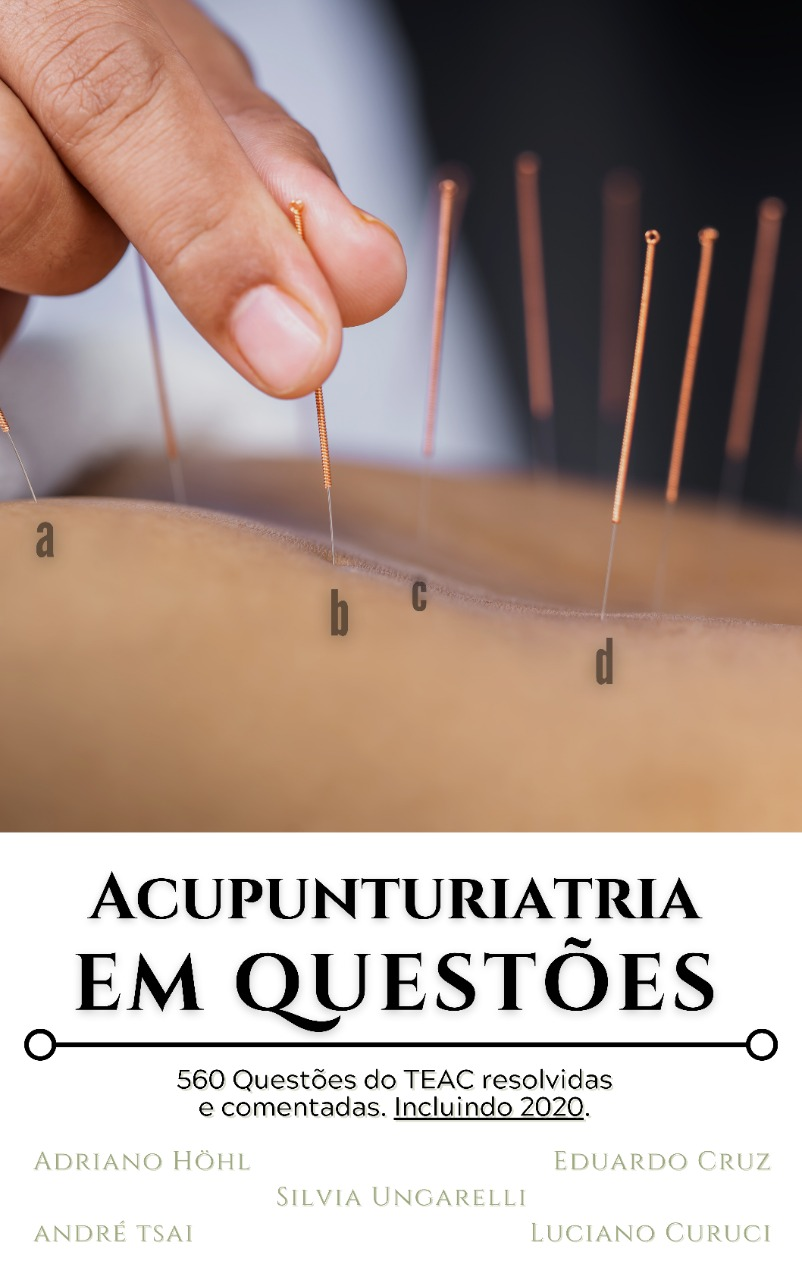
\includegraphics[width=6.5cm,height=8.5cm]{pix/coverimg.jpg} %[0.2cm]
			% title
			%{ \huge \bfseries Acupuntura Médica em Questões} \\%[0.1cm]
			%\HRule \\[0.2cm]
			
			% Optionally translator and publishing house
			% The Translator
			%\begin{minipage}{0.4\textwidth}
			%\begin{flushleft} \small
			%\emph{Translated by:}\\
			%Good Translator %here the translator
			%\end{flushleft}
			%\end{minipage}
			% Publishing House
			%\begin{minipage}{0.2\textwidth}
				%\begin{flushright} \small
			%	\begin{flushleft} \small
					%\emph{Edição:} \\
					%\textsc{Eduardo Cruz} % here the publishing house
				%\end{flushleft}
			%\end{minipage}
		\end{center}
	\end{titlepage}
	
	
	
	%%%SIMPLE TITLEPAGE
	\maketitle 
	\thispagestyle{empty}
	\clearpage
	\setcounter{tocdepth}{6}
	
	%TOC
	\tableofcontents
	\listoftables
	%TUTAJ PISZ ALBO ZROB \INCLUDE{} LUB \INPUT{}


	%\input{lorem.tex}
%	\part{Questões separadas por assunto}
%	\chapter{Pontos de acupuntura}
%	\begin{itemize}
%	\item \noindent	\hyperlink{pontos 1}{2013-01}\\
%	\item \hyperlink{pontos 2}{2013-02}\\
%	\item \hyperlink{pontos 3}{2013-03}\\
%	\item \hyperlink{pontos 4}{2013-04}\\
%	\item \hyperlink{pontos 5}{2013-05}\\
%\end{itemize}

	
	
%\part{Capítulos introdutórios}	
%\pagestyle{empty}


\chapter*{Sobre os autores}

Adriano Höhl
\begin{itemize}
	\item Graduação em Medicina pela Faculdade  de Medicina da Universidade Federal de Goiás
	\item Especialista em  Acupuntura Médica pelo Colégio Brasileiro de Acupuntura Médica e Associação Médica Brasileira .
	\item Especialista em  Nutrologia pela Associação Brasileira  de Nutrologia e   Associação Médica Brasileira.
	\item Especialista em  Ginecologia e Obstetrícia  pela  FEBRASGO e Associação Médica Brasileira. 
	\item Título de Habilitação em    Ultrassonografia Ginecológica pela FEBRASGO e Colégio Brasileiro de Radiologia.
	\item Título de habilitação em Densitometria  pelo Colégio Brasileiro de Radiologia.
	\item Diretor Clínico da Höhlklinik
\end{itemize}


Silvia Ungarelli
\begin{itemize}
	\item Graduação em Medicina pela Faculdade de Medicina da Universidade Federal de Goiás.
	\item Especialista em Acupuntura Médica pelo Colégio Brasileiro de Acupuntura Médica e Associação Médica Brasileira.
\end{itemize} 

Eduardo Cruz
\begin{itemize}
	\item Graduação em Medicina pela Faculdade de Medicina da Universidade Federal de Goiás.
	\item Especialista em Ginecologia e Obstetrícia pelo Hospital das Clinicas da Universidade Federal de Goiás.
	\item Especialista em Acupuntura Médica pelo Colégio Brasileiro de Acupuntura Médica e Associação Médica Brasileira.
\end{itemize}
% Capítulos introdutórios
\chapter*{Dedicatórias}


\textit{Dedicatórias :}

\textit{Dedico este livro a minha esposa Ana Lúcia, a minha mãe Luzia e a meus filhos Laura e Luisa, Adriano Filho e  Mariana.
Adriano Höhl}




\textit{Dedico este livro a minha esposa Tânia Mara, aos meus filhos Gabriel, Eduardo e Hugo.}


\textit{Eduardo Cruz }\\

\textit{Dedico este livro à minha querida família.}

\textit{Silvia Ungarelli}\\




\textit{Dedicamos este livro  a todos os  Colegas e professores  do  V Curso de Acupuntura do CMA-Goiás.}
\textit{Adriano, Eduardo e Silvia}



\chapter*{Prefácio}

\textit{O estudo da Acupuntura médica  e bastante difícil e ao mesmo tempo encantador. 
	Iniciamos os  estudos na  Medicina Tradicional Chinesa ainda no ano de 2017, em Goiânia, onde descobrimos uma nova forma de ver a medicina em sua forma mais antiga da história. Deixamos para trás toda a tecnologia e toda a complexa farmacologia, potencializamos a nossa imaginação em busca deste conhecimento novo e de uma nova teoria que  para muitos parece tão abstrata. Um paradoxo entre uma Medicina tãoo simples, mas ao mesmo tempo tão complexa e que funciona tão bem que, com o tempo, nos mostrou a grande verdade do pensamento de Leonardo da Vinci quando diz: “A Simplicidade é o último grau de Sofisticação.” A ideia desta obra surgiu durante a nossa especialização, em meio a dificuldades cotidianas como tempo para estudo, trabalho, compromissos familiares e o preparo para o esperado TEAC - prova de título de especialista em Acupuntura Médica, promovida pelo Colégio Médico Brasileiro de Acupuntura. A semente do trabalho foi plantada e germinada pela união e reunião de um grande número de alunos, até então especializandos. Neste momento, ainda alunos, reunimo-nos, dividimos e sistematizamos 12 anos de provas de título, para que assim pudéssemos compartilhar entre nós mesmos as questões comentadas que facilitariam nosso estudo. O resultado da metodologia veio com a aprovação de 98\% da turma do CMA-Goiás, todos com médias de notas altas, além  da conquista  da primeira nota 10 em toda a história da prova de títulos  em Acupuntura Médica, feito alcançado por um dos autores desta obra, a Dra. Silvia Ungarelli.
	Em Janeiro de 2020 selecionamos os  últimos 07 anos e resolvemos refazer todas as questões de forma diferente, visando padronizar, aprimorar a didática, com respostas mais completas  de uma forma que  o conteúdo  possibilitasse aos novos especializandos, usufruir deste nosso trabalho e aos  médicos acupunturiatras,  revisar alguns assuntos específicos.  
	Logo no mês de   Março,  fizemos um contato com o Dr André Tsai, que havia nos dado aula na especialização, apresentando o trabalho iniciado e ele então, nos apresentou  o Dr Luciano Curuci, também professor  nos cursos de acupuntura,  e  daí então trabalhamos juntos  até a conclusão do  livro. 
	No ultimo, mês de janeiro após concluídas as revisões, resolvemos  adicionar a última prova de 2020, a fim de tornar a obra mais completa e atualizada.  
	Ressaltamos a importância do estudo sistematizado nos tratados e na referência bibliográfica de cada curso, pois nosso objetivo nunca foi substituí-los e sim proporcionar uma ferramenta a mais para o entendimento e fixação do aprendizado, preparando para provas e concursos que o leitor possa participar. 
	Assim, a obra está organizada por questões e no Índice Remissivo pode-se pesquisar por temas, indo direto às questões existentes. 
	Esperamos que aproveitem e que Gostem.}

\pagestyle{plain}


\part{Provas do TEAC} Questões resolvidas e comentadas.




\chapter{TEAC 2013} TEAC 2013
\index{pontos}
\subsubsection{QUESTÃO 01} - Usado para o tratamento da cefaleia e do torcicolo. Anatomicamente localizado em uma depressão entre o músculo esternocleidomastoideo e trapézio e, em posição profunda, no músculo esplênio da cabeça. Suprido pela artéria occipital e por um ramo do nervo occipital menor. Estamos nos referindo a qual ponto?  \\

a) Du Mai 16 \\
\textit{Situa-se na nuca, sob a protuberância occipital externa, na linha mediana do corpo, ou a um tsun acima da linha de inserção dos cabelos. Relaciona-se com os ramos cutâneos do nervo occipital terceiro (C) e com o nervo occipital maior (C2), ambos provindos do ramo dorsal.}\\
b) TA 17 \\
\textit{Situa-se posteriormente ao lóbulo da orelha, em uma depressão interóssea, localizada entre o processo mastoideo e o ramo da mandíbula. Relaciona-se, superficialmente, com o nervo auricular magno (plexo cervical) e, profundamente, com os nervos auriculotemporal (ramo do nervo trigêmeo) e com o nervo facial.}\\
c) VB 12 \\
\textit{Situa-se em uma reentrância óssea localizada posterior e abaixo do processo mastóideo. Fletir o pescoço para sua determinação. Relaciona-se com o nervo occipital menor (plexo cervical - C2).}\\
d) VB 20 \\
\textit{Trata-se de VB 20 que se situa em uma depressão óssea localizada entre o músculo esternocleidomastoideo e a inserção superior do músculo trapézio, ou na reentrância óssea localizada entre a protuberância occipital externa e o processo mastóideo ao nível de Du 16. Relaciona-se com o nervo occipital maior.}\\
 
\textbf{A alternativa correta é a letra D.}\\

\index{pontos}
\subsubsection{QUESTÃO 02} - Proximal ao processo estilóide do rádio, entre os tendões dos músculos braquiorradial e abdutor longo do polegar. Suprido pela veia cefálica e ramos da artéria e veia radial, inervado por um ramo do nervo cutâneo lateral do antebraço braço e por um ramo superficial do nervo radial. Indicado para disfunções respiratórias e dor de cabeça. Que ponto é esse?  \\

a) P 10  \\
\textit{Situa-se no meio do 1º metacarpo na linha da mudança da cor da pele. Relaciona-se com nervo cutâneo lateral do antebraço superficialmente e mediano profundamente.} \\
b) IG 5  \\
\textit{Situa-se numa reentrância no fundo da tabaqueira anatômica. Relaciona-se com o nervo radial.}\\ 
c) P 7  \\
\textit{Situa-se um e meio tsun proximais à prega ventral do punho, lateralmente a artéria radial. Relaciona-se com nervo radial.}\\
d) IG 4 \\
\textit{Situa-se na metade do 2º metacarpo entre o primeiro e o 2º metacarpo. Relaciona-se com nervo mediano superficialmente e com o ulnar profundamente.} \\
 
\textbf{A alternativa correta é a letra C.} \\ 
\index{pontos}

\subsubsection{QUESTÃO 03}- Ponto com indicação ampla para enfermidades do baixo ventre, digestivas, urinárias e ginecológicas. Localizado a 3 cun inferior à cicatriz umbilical. Suprido pela artéria e veia epigástricas inferiores e por um ramo cutâneo anterior medial do nervo intercostal. A que ponto nos referimos? \\
a) Ren Mai 4 \\
\textit{Trata-se de VC 4, ponto de saída dos três Yin do pé e ponto que harmoniza o   Aquecedor inferior, localizado na linha mediana anterior, 2 cun cranialmente à margem superior da sínfise púbica e 3 cun caudalmente ao umbigo. Fortalece e nutre os rins, o Jing, o útero, sendo importante em doenças ginecológicas e urológicas, fraqueza, dores e frio na região lombar, diarréia, incontinência fecal.} \\
b) R 13 \\
\textit{Situa-se a 3 tsun abaixo do centro da cicatriz umbilical e 0,5 tsun lateral à linha média anterior.}\\
c) F 14 \\
\textit{Situa-se a 4 tsun laterais à linha média anterior, no sexto espaço intercostal.}\\
d) E 29 \\
\textit{Situa-se a 4 tsun abaixo do centro da cicatriz umbilical e 2 tsun laterais à linha média anterior.}
 \\
\textbf{A alternativa correta é a letra A.}\\
\index{pontos}
\subsubsection{QUESTÃO 04} - Localizado no dorso da mão, entre o segundo e terceiro metacarpianos. Anatomicamente está situado no músculo interósseo do segundo metacarpiano, diretamente acima do nervo, artérias e veias digitais dorsais e palmares comuns, bem como do arco palmar profundo e ramos terminais profundos do nervo ulnar. Indicado para torcicolo, cefaleia, dor no ombro e braço. Qual dos pontos enumerados abaixo corresponde às referidas características? \\

a) Yaotongxue (ponto extra) \\
\textit{Localizam-se entre o 2º e 3º e entre o 4º e 5º metacarpos, na altura do corpo para a base. Indicado nas lombalgias agudas.}\\
b) IG 3 \\
\textit{Situa-se em margem lateral (radial) do 2º metacarpo, em uma reentrância proximal à articulação metacarpofalângica. Na camada superficial, relaciona-se com os nervos digitais dorsais do ramo superficial do nervo radial e com os nervos digitais palmares próprios do nervo mediano.} \\
c) Baxie (ponto extra) \\
\textit{Localiza-se entre as cabeças dos metacarpos. Relaciona-se com os ramos cutâneos e musculares dos nervos radial e ulnar. Indicado nas doenças articulares dos dedos, paresia dos dedos, cefaleia, torcicolo, dor de dente, garganta inflamada.} \\
d) Luozhen (ponto extra) \\
\textit{O próprio nome significa torcicolo.  É um dos pontos extras importantes, situando-se no dorso da mão, meio tsun entre as cabeças do 2º e 3º metacarpos. Relaciona-se com os nervos digitais dorsais do nervo radial.} 

\textbf{A alternativa correta é a letra D.}\\ 
\index{pontos}
\subsubsection{QUESTÃO 05}- Localiza-se na margem posterior do côndilo medial do joelho, na parte anterior da inserção dos músculos semimembranoso e semitendinoso e na margem do músculo sartório. Tem indicações no tratamento de disfunções do joelho, impotência sexual, vaginite. Que ponto é esse? 

a) BP 8 \\
\textit{Situa-se a cinco tsun distais à interlinha articular do joelho, sobre a margem medial da tíbia, ou a três tsun distais ao BP-9. Indicado em lombalgia, meteorismo, distensão abdominal e dos lados do abdome, dismenorreia, menorragia, menstruações irregulares, edema, polução noturna, dificuldade de micção e em todos os casos de formação ou de aumento da forma (tumores benignos, malignos, obesidade, artrose, etc). }
b) F 8 \\
\textit{Situa-se na face medial do joelho, na extremidade medial da prega poplítea, em uma depressão entre o tendão do músculo semitendíneo e o côndilo medial da tíbia. Para localizar o ponto, deve-se fletir o joelho e abduzir o membro inferior. Indicado nas afecções geniturinárias, vaginite, prostatite, nefrite, afecções do joelho, hemorragias intestinais, prolapso uterino, dores no baixo-ventre, disúria, prurido vulvar, dor no pênis, patologias hepáticas e biliares.}
c) R 10 \\
\textit{Situa-se à margem medial da fossa poplítea, na prega poplítea, tangente à margem lateral do tendão do músculo semitendíneo. Faz a limpeza do Calor Perverso do Aquecedor Inferior e do Calor do Xue. Harmoniza o Qi contracorrente e é o ponto que rege as membranas.}\\
d) BP 9 \\
\textit{Situa-se em uma reentrância óssea que se encontra sob a margem inferior do côndilo medial da tíbia e o músculo gastrocnêmio. Indicado em todas as afecções encontradas na parte alta e interna do corpo, ocasionadas pela lesão da Energia Yin, plenitude nos lados do abdome, ascite ou edema, enurese noturna, incontinência urinária, espermatorréia, menstruação irregular, disenteria, distensão do abdome, retenção urinária, infecção urinária, gonalgia, dor nos genitais externos e lombalgia.} \\

\textbf{A alternativa correta é a letra B.}\\
 \index{Canais Maravilhosos}
 \index{Vasos Maravilhosos}
\subsubsection{QUESTÃO 06}- Os Canais Extraordinários se ramificam e intersectam um ou mais canais principais. A sintomatologia dos mesmos não é exclusiva, decorre de uma combinação de sintomas clínicos associados aos canais principais a que se ligam. O tratamento de doenças que afetam estes canais se faz através de pontos dos meridianos principais relacionados.
 Nesse sentido, é correto afirmar que: 
\\
a) As doenças febris são comumente associadas ao Du Mai (Vaso Governador), e o principal ponto de interseção usado para seu tratamento é o Du 26. \\
\textit{O correto seria Yang Wei Mai que se conecta aos três meridianos Yang do Pé e da Mão, com o Tai Yang, que controla a superfície do corpo e com o Shao Yang que tem relação com a síndrome intermediária. Esta é a razão da presença de frio ou febre quando há disfunção do Yang Wei Mai.}  \\
b) Pelo fato do Du Mai suprir o cérebro e a região espinhal e intersectar o canal do Fígado no vértice, a obstrução do Qi neste canal pode resultar em sintomas como rigidez e dor ao longo da coluna vertebral. \textit{Na verdade, Du Mai recebe todos os canais yang da mão e do pé no vértice, em Du 20. Du Mai percorre a parte posterior do corpo e entra no cérebro. Uma anormalidade no Qi do Du Mai causa dor intensa ao longo da coluna vertebral e sensação de peso na cabeça.} \\
c) O Canal Yin Wei Mai (Vaso Conexão) é um dos canais que mais se relaciona com infertilidade e distúrbios do sistema urogenitais. \\
\textit{O Canal seria Ren Mai que nutre e regula todos os meridianos Yin. No corpo humano, Qi pertence a Yang e Xue a Yin. A gestação, o parto, a menstruação e o corrimento vaginal estão intimamente relacionados a Xue (Yin), portanto dizemos que "o Ren Mai se encarrega do feto".} \\
d) O Canal Yang e Yin Qiao Mai (canal Yang e Yin do calcanhar) teem em comum a função de regular o movimento dos membros superiores. \\
\textit{Na verdade, controlam membros superiores e inferiores. Yin Qiao Mai e Yang Qiao Mai controlam Yin e Yang em ambos os lados dos membros. O Yang Qiao Mai controla Yang Qi, enquanto o Yin Qiao controla Yin Qi. Eles controlam os meridianos Yin e os meridianos Yang nas faces medial e lateral da perna.} \\

 
\textbf{A alternativa correta é a letra B.}\\ 
\index{dor!cervicalgia}
\subsubsection{QUESTÃO 07}- Paciente de 42 anos queixa-se de dor aguda no pescoço e ombro, que piora com os movimentos. Acompanha-se de cefaleia cervical ou occipital. Diz que essa situação o está deixando irritado, com dificuldade para conciliar o sono e um tanto fadigado. Ao exame físico não apresenta nenhuma deformidade, no entanto, os movimentos ativos do pescoço são limitados e dolorosos. À palpação nota-se tensão muscular em trapézio e músculos paraespinhais. Radiografia em AP e perfil revelam alterações de espaço intervertebral e osteófitos entre C5 e C6 e C6 e C7. Na sua avaliação, qual seria o diagnóstico provável e a prescrição de pontos mais adequada para este caso? \\

a) Hérnia de Disco Cervical; ponto principal extra Luozhen e pontos complementares: IG 4 e VB 38. \\
\textit{Apesar de citar alterações do espaço intervertebral, a alteração é aguda, mostra comprometimento muscular e faltam dados concretos na clínica como sintomas de dor irradiada ou parestesias além de exames de imagem mais precisos que possam confirmar hérnia de disco cervical.} \\
b) Torcicolo ou Entorse Cervical; ponto principal extra Luozhen; pontos complementares: ID3 e VB 39. \\
\textit{Corresponde ao torcicolo por contrações dolorosas da musculatura do pescoço, com limitação à rotação para um dos lados e posição antálgica. Segundo a MTC, essa alteração é causada por invasão de vento frio nos meridianos e colaterais locais ou pela estagnação de Qi e Xue ocasionada pela má posição da cabeça ao dormir ou trauma do pescoço ao esforço.  O tratamento visa à eliminação de vento e frio patogênicos e desobstrução dos meridianos.  
Lao Zhen (ou Luozhen) é um ponto extra que movimenta o Qi e o Xue na região do pescoço. O ID 3 é o ponto de confluência do intestino delgado com o Du Mai e o VB 39 é o ponto de influência da medula. Associados, podem regularizar o Qi e o Xue, relaxar os tendões e colaterais e promover analgesia.} \\
c) Luxação da Coluna Vertebral; ponto principal: Extra Yaotongxue; pontos complementares: ID 5 e VB 34 \\
\textit{Não existe história de trauma e nem mesmo alterações de imagem que possam reforçar esta hipótese.}  \\
d) Espondilite Anquilosante; ponto principal extra Taiyang; pontos complementares: TA 5 e VB 34. \\
\textit{Na espondilite anquilosante, a história é de evolução crônica e não aguda, acometendo mais de um segmento da coluna.  Não existem dados nas histórias que possam enquadrar o paciente nos critérios.} \\
 
\textbf{A alternativa correta é a letra B.}\\
\index{dor!lombalgia}
\subsubsection{QUESTÃO 08}- Paciente do sexo masculino, 42 anos, queixa-se de dor de instalação insidiosa há cerca de um ano. Trata-se de uma dor difusa, em peso, localizada na região lombosacra, sem irradiação para os membros inferiores, que melhora pelo repouso e exacerba-se aos esforços. À palpação,nota-se a musculatura da região lombosacra difusamente dolorida e reflexos profundos dos MMII sem alterações. Levando-se em consideração que a radiografia da coluna lombosacra foi de grande auxílio na elucidação diagnóstica, é correto afirmar, que nesse caso o diagnóstico e os pontos de acupuntura principais para o tratamento são respectivamente: \\
  
a) Fratura de Vértebra Lombar. Pontos principais: B 40 e B 37   \\
\textit{Trata-se de dor de duração de 1 ano, envolvendo região lombosacra, em paciente jovem sem história de trauma, a qual teria uma evolução de melhora ou de complicação devido a etiologia mais agressiva como metástase, mas não evolução tão arrastada. Não seria a primeira opção de diagnóstico.} \\
b) Estenose de Canal Medular. Pontos principais: B 40 e VB 34  \\
\textit{No estreitamento do canal raquidiano artrósico, a dor lombar, às vezes, é noturna; outras vezes, a ela se associa ciatalgia uni ou bilateral intensa, que melhora ao sentar-se. Pode ser acompanhada de dor na panturrilha e de claudicação neurogênica intermitente. O processo doloroso piora ao caminhar, principalmente ladeira abaixo, e melhora ladeira acima, o que a diferencia da claudicação vascular, que piora ladeira acima.} \\
c) Tuberculose Espinhal. Pontos principais: B 40 e B 39   \\
\textit{A tuberculose espinhal geralmente se acompanha de sinais e sintomas próprios do processo infeccioso como febre baixa vespertina e evolução consumptiva, com progressão para   as vértebras vizinhas e aparecimento de comprometimento neurológico, o que não condiz com a história.} \\
d) Discopatia Degenerativa Lombar. Pontos principais: B 40 e B 60   \\
\textit{A discopatia degenerativa pode evoluir com a herniação do disco intervertebral para o canal espinhal, evoluindo ou não com sinais e sintomas neurológicos, conforme o grau de comprometimento da compressão de raízes nervosas. O fato de a dor melhorar com o repouso e piorar com as atividades físicas reforça a hipótese. Sob a óptica da MTC, trata-se de uma lombalgia Shao Yin que piora com fadiga, esforços físicos, mental e/ou sexual. O Tratamento baseia-se no uso de pontos locais associados a pontos à distância como R 2, R 3, B 40, B 60.  
O ponto B 40 é clássico para lombalgias e dorsalgias, podendo ser associado a B 60, B 23 e Yaoyan.} \\
 
\textbf{A alternativa correta é a letra D.}\\
\index{dor!ombralgia}
\subsubsection{QUESTÃO 09}- Paciente do sexo feminino, 40 anos, procura o ambulatório de acupuntura para tratamento de dor no ombro direito iniciada há cerca de um ano. Caracteriza-se por dor em pontada, de forte a moderada intensidade que piora ao movimento de abdução e irradia-se para a face anterolateral do braço (apresenta restrições aos movimentos ativos). Não apresenta parestesia ou choques. O sono é prejudicado devido ao agravamento da dor quando se deita sobre o lado comprometido. A radiografia do ombro mostra o acrômio curvado ou ganchoso, com diminuição do espaço da articulação glenoumeral. Na sua avaliação qual o diagnóstico mais provável? E qual é o melhor esquema de pontos para tratamento deste ombro doloroso? \\

a) Hérnia Discal Cervical. Pontos principais: IG 14, IG 16, ID 8, TA 14, Extra Jianneiling. \\
\textit{Nos casos de hérnia discal cervical teremos a descrição de uma neuralgia, com características diferentes da dor apresentada no caso acima, em que não há descrição de comprometimento neurológico.} \\
b) Capsulite Adesiva. Pontos principais: IG 16, ID 9, TA 14, Extra Jianneiling. \\
\textit{A capsulite adesiva ou ombro congelado é um quadro clínico caracterizado por dor difusa em todo o ombro, que piora no período noturno e está associada a rigidez da articulação do ombro, com limitação de movimentos ativos e passivos. A história descrita não cita rigidez do ombro, mas apenas que há limitação ativa da articulação.}\\
c) Síndrome do Impacto. Pontos principais: IG 15, IG 16, ID 11, TA 14, Extra Jianneiling. \\
\textit{A alteração radiológica descrita é característica da síndrome do impacto tipo III. Sob a óptica da MTC, trata-se de uma ombralgia por estagnação do Qi e Xue nos meridianos Yang da mão. Os pontos locais de escolha podem ser IG 15, TA 14, ID 9, ID 10, IG 16, Naoshang, Jianneiling e ID 11, que são aplicáveis ao tratamento de todos os tipos de ombralgias, com a finalidade de aumentar o Qi Correto e dissipar os agentes perversos.} \\
d) Instabilidade Glenoumeral. Pontos principais: IG 12, IG 16, ID 11, TA 14. \\
\textit{Na história não há descrição de luxação do úmero com dor intensa, associada a incapacidade de movimentar o braço, nem mesmo informação de que o paciente tem a sensação de que algo “saiu do lugar”.}\\

\textbf{A alternativa correta é a letra C.}\\
\index{dor!coxalgia}
\subsubsection{QUESTÃO 10}- Paciente do sexo feminino, 32 anos, refere dor e disestesia na face lateral da coxa há 2 meses. A dor se irradia até a face lateral do joelho e, mais raramente, para a virilha ipsilateral. Tem a sensação de choque quando estende o quadril afetado. Ao exame físico não apresenta sensibilidade significativa ao nível do trocânter maior, nem restrições na rotação interna do quadril. Os reflexos nos membros inferiores são presentes e simétricos e as radiografias da pelve e quadril não mostram alterações. Analisando o quadro acima, qual seria a hipótese diagnóstica e a conduta adequada, respectivamente? \\

a) Trata-se de um quadro de hérnia discal lombar e o meridiano comprometido é o do Baço \\
\textit{Mesmo que se tratasse de uma hérnia discal, patologia que cursa geralmente com alteração dos reflexos e da sensibilidade, além da dor, o meridiano comprometido não seria o do Baço, por este ser medial, e sim o da Vesícula Biliar.}\\ 
b) Trata-se de um quadro de osteoartrite do quadril e o meridiano comprometido é o da Bexiga \\
\textit{Pela localização da dor e disestesia ser na face lateral, o meridiano comprometido é o da Vesícula Biliar.} \\
c) Trata-se de um quadro de bursite trocanteriana e os principais meridianos afetados são Estômago e Fígado. \\
\textit{O Quadro clínico não é compatível com a bursite trocantérica, que se caracteriza por dor crônica intermitente acompanhada de desconforto à palpação da região lateral do quadril e não de parestesia. A dor localizada à palpação do grande trocânter, área de inserção do tendão do glúteo médio, pode ser encontrada em todos os pacientes sintomáticos e pode ser reproduzida pela abdução ativa resistida e pela rotação externa da articulação, havendo a possibilidade de ser provocada ocasionalmente pela rotação interna. Como o comprometimento é da face lateral da coxa, o comprometimento é do meridiano da Vesícula Biliar.} \\
 
d) Trata-se de um quadro de meralgia parestésica; o principal meridiano afetado é o da Vesícula Biliar \\
\textit{Trata-se realmente de um caso de uma mononeuropatia, mais especificamente a Meralgia Parestésica, patologia que se deve à compressão do nervo cutâneo lateral. Muito comum em mulheres atletas, se manifesta com sensações como dormência, formigamento, queimação, frio e dor nesta região da coxa. Além disso, há redução da sensibilidade e hipersensibilidade ao toque na região afetada, cujo tratamento é clínico conservador, associado à fisioterapia.  
Sob a óptica da MTC, por afetar a região lateral da coxa, trata-se de provável estagnação ou obstrução do meridiano da Vesícula Biliar, devendo-se usar pontos locais e à distância, visando estabelecer a circulação de Qi e Xue.} \\
 
\textbf{A alternativa correta é a letra D.}\\ 
\index{dor!coxalgia}
\subsubsection{QUESTÃO 11}- Paciente do sexo masculino, 40 anos, procura ambulatório de acupuntura referindo dor no quadril esquerdo há um ano. A dor é de forte intensidade, em pontada e contínua, com irradiação para face lateral da coxa; piora ao movimento de levantar e sentar, e melhora quando deambula por pouco tempo (piora se permanecer andando por longo tempo). Não consegue dormir, pois a dor agrava quando se deita sobre o lado afetado. Ao exame físico, apresenta claudicação com a deambulação, sinal de Trendelenburg positivo, sensibilidade dolorosa aumentada acima da face lateral do trocânter e ausência de pontos gatilhos palpáveis. Não apresenta dor à rotação interna, mas refere dor discreta à rotação externa do quadril. Ao exame neurológico, os reflexos dos MMII estão presentes e simétricos. Radiografias da pelve e quadril esquerdo mostram a presença de osteófitos na face lateral do trocânter. Qual o diagnóstico provável e a prescrição de pontos mais apropriados para essa nosologia?\\
  
a) Síndrome dolorosa miofascial do músculo piriforme; pontos: VB 31, VB29, VB 25  \\
\textit{O caso não se enquadra na síndrome dolorosa miofascial do músculo Piriforme. A síndrome do piriforme (SP) é uma importante causa de dor na região glútea que pode frequentemente ser acompanhada de ciatalgia. Atualmente é descrita como uma forma de encarceramento do nervo isquiático que causa dor desde a região glútea à área de distribuição deste nervo, representando uma entidade clínica configurada não somente pela presença do quadro álgico, mas também por distúrbios sensitivos, motores e tróficos relacionados à distribuição radicular do nervo isquiático.} \\
b) Tendinite do tendão do glúteo médio; pontos: VB 30, VB 29, VB 39  \\
\textit{Na tendinite do músculo glúteo médio, a dor localiza-se na região do quadril (sobre o trocânter do fêmur), pode irradiar-se pela face lateral da perna e piora ao ficar muito tempo em pé, ao subir e descer escadas, ao caminhar ou ao correr. Pela localização do quadro álgico, trata-se de comprometimento do Meridiano da Vesícula Biliar, podendo ser usados pontos locais VB 29, VB 30 e pontos à distância como VB 34. O teste de Trendelenburg é um exame físico rápido que pode ajudar o terapeuta a avaliar qualquer disfunção do quadril. Um teste de Trendelenburg positivo geralmente indica fraqueza nos músculos abdutores do quadril: glúteo médio e glúteo mínimo. Um teste positivo é aquele em que a pélvis cai no lado contralateral durante uma perna única no lado afetado. Isso também pode ser identificado durante a marcha: a compensação ocorre ao lado flexionando o tronco em direção ao lado envolvido durante a fase de apoio na extremidade afetada.}\\
c) Meralgia parestésica; pontos: VB 29, B 23, VB 34  \\
\textit{No caso da meralgia parestésica, o principal sintoma é a parestesia, em virtude da compressão nervo cutâneo lateral da coxa.} \\
d) Lombociatalgia; pontos: B 23, B 25, VB 30, VB 31, VB 41  \\
\textit{No caso da lombociatalgia, a dor inicia-se na região lombar e se irradia pelo trajeto do nervo ciático, ou seja, região glútea, posterior da coxa e perna podendo lateralizar ou medializar distalmente até o pé na dependência do dermátomo comprometido (raiz correspondente). A dor ciática é relatada pelos pacientes como “ferroada”, “fisgada” ou “sensação de choque” associada a parestesias e graus variados de déficit motor do(s) membro(s) inferior(es) bem como marcha claudicante. A associação com postura antálgica da coluna lombar em escoliose ou posição em flexo lombar é comum. A dor tem características mecânicas: piorando aos movimentos e esforços em geral e atenuando em repouso, posição fetal ou decúbito dorsal com quadris e joelhos fletidos. Há exacerbação da dor também à manobra de Valsalva (tosse, espirros e esforços para evacuação).}\\

\textbf{A alternativa correta é a letra B.}\\ 
\index{dor!plantalgia}
\subsubsection{QUESTÃO 12}- Paciente do sexo feminino, 50 anos, queixa-se de dor localizada logo acima da tuberosidade medial do calcâneo esquerdo há oito meses. A dor melhora com repouso e é mais intensa ao despertar, quando dá os primeiros passos. Apresenta sensibilidade dolorosa 1 a 2 cm, distalmente, ao longo da fáscia plantar. A radiografia lateral do pé esquerdo para diagnóstico diferencial não mostrou nenhuma relevância. Qual o diagnóstico, a técnica e os pontos a serem prescritos? \\
a) Fasciíte plantar. Os principais pontos são os dolorosos locais. Caso não melhore a dor, se faz uso dos pontos complementares: B 57, R 3 e B 60, com estímulo moderado a forte. \\
\textit{Trata-se de um quadro clássico de fasciíte plantar, condição crônica caracterizada por dor na região plantar do terço posterior dos pés, dor à compressão da tuberosidade medial do calcâneo e história de dor nos primeiros passos do dia. Tratamento com AINES, palmilhas e acupuntura. Os pontos mais usados são: R 3, B 60, B 57 e pontos locais.} \\
b) Síndrome do túnel tarsiano. Os pontos principais são: B 57, R 1 e B 60. Caso não melhore a dor, usam-se os pontos complementares, que são os pontos dolorosos locais, com estímulo moderado a forte. \\
\textit{Na síndrome do túnel do tarso, a dor é retromaleolar em queimação ou formigamento e algumas vezes no calcanhar plantar medial, podendo se estender-se ao longo da superfície plantar, bem como nos dedos dos pés. Embora a dor piore durante a permanência em pé e ao caminhar, pode ocorrer dor em repouso, o que a diferencia da fasciíte plantar. Sendo patologia de acometimento medial, presume-se o comprometimento dos meridianos Yin do Pé e pela topografia haveriam pontos mais indicados para o tratamento, como R 3, R 7, BP 4, BP6, entre outros.}\\ 
c) Ruptura traumática aguda da fáscia plantar; os pontos principais são: B 57, R 3 e B 62, não havendo indicação para o uso de pontos dolorosos locais devido a lesão da fáscia \\
\textit{Na ruptura traumática aguda da fáscia plantar a dor é de aparecimento súbito, acompanhada de uma sensação de clique. Geralmente localiza-se na região medial da planta, afastada do calcanhar, com uma grande sensibilidade ao toque e dificuldade na marcha, acompanhada de edema e equimose ao longo da borda medial do pé.} \\
d) Osteoartrose da articulação do tornozelo; os pontos principais são: B 57, R 9 e B 60. Caso a dor não melhore, se faz uso dos pontos dolorosos locais com estímulo moderado a forte \\
\textit{A osteoartrite da articulação tíbio társica cursa com dor na interlinha articular, associada ou não a aumento de volume (derrame articular) e limitação da amplitude de movimento articular, da função, do trabalho e das atividades de lazer. A etiologia pós-
traumática é a principal causa da osteoartrite de tornozelo. Ao exame radiológico, pode-se constatar diferentes graus de diminuição do espaço articular e formação de osteófitos, esclerose e cistos subcondrais.}  \\
\textbf{A alternativa correta é a letra A.}\\ 

\index{dor!gonalgia}
\subsubsection{QUESTÃO 13}- Paciente com 40 anos, sexo feminino, com dor no joelho direito há um ano, foi encaminhada ao serviço de acupuntura pelo fato de não haver obtido melhora com uso de AINHs, corticoides e fisioterapia. Informa que a dor piora ao levantar pela manhã ou depois de um período de exercício contínuo, caminhadas ou corrida, fatores que a levam a claudicar. Localiza-se na face medial do joelho, ao nível da inserção conjugada dos músculos isquiotibiais. Ao exame físico não há restrições de movimentos, porém a movimentação do joelho é dolorosa. Não há instabilidades, travamentos ou outros sintomas mecânicos. As radiografias em AP, perfil e axiais não apresentaram alterações relevantes. Levando em consideração o quadro acima, podemos afirmar:  \\

a) Não deixa dúvidas que estamos diante de um quadro de artrite reumatóide de joelho. A acupuntura não trará benefícios à paciente, pois o tratamento indicado deve ser feito a base de metotrexato e hidroxicloroquina \\
\textit{Apesar da rigidez matinal, não há sinais flogísticos e nem sorologia para que se possa confirmar o diagnóstico, nem tão pouco alterações radiológicas. Ainda que fosse, poderiam ser usados pontos de acupuntura para diminuição do processo inflamatório e da dor.} \\
b) O quadro clínico fecha o diagnóstico de tenossinovite de joelho. Os pontos indicados neste caso são: E 35 e Xiyan medial, B 40 e pontos dolorosos locais. \\
\textit{O diagnóstico de tenossinovite é a principal suspeita diagnóstica pois cursa com dor à palpação da inserção muscular e que piora com atividade física, porém sem limitação da mobilidade, o que faz pensar em patologia extra-articular. Os pontos E 35, Xiyan medial e B40 são excelentes opções de associação de pontos locais para afecções de partes moles do joelho.} \\
c) Neste caso, é indispensável a RNM para afastar laceração de menisco medial que, caso comprovada, terá indicação imediata de cirurgia.  \\
\textit{A RNM é um exame de diagnóstico que poderá ser precedido pela radiografia e também pela ultrassonografia. Geralmente, no caso de lesão de menisco, ocorrem sinais flogísticos de dor e edema além da restrição de movimento.  O tratamento pode variar de fisioterapia até cirurgia, sendo a última terapia de exceção, não sendo de indicação imediata.} \\ 
d) Trata-se de um caso clássico de osteoartrite de joelho. Os pontos indicados são: E 35, E 36, Extra Heding e BP6. \\
\textit{A ausência de alterações radiológicas e instabilidades já afastaria a hipótese de osteoartrite de joelho.}  \\

\textbf{A alternativa correta é a letra B.}\\
\index{Síndrome Bi}
\subsubsection{QUESTÃO 14}- Paciente de 43 anos, com queixa de dores articulares há cerca de dois meses. Informa que a dor surgiu de forma insidiosa, tem caráter migratório e de forma simétrica nas pequenas articulações (mãos e pés) e grandes articulações (tornozelos e joelhos). Apresenta rigidez articular prolongada, que é pior pela manhã, bem como aumento do volume articular. Sente-se fadigada e tem aversão ao frio. Ao exame físico, as articulações apresentam-se com edema, principalmente as articulações interfalangeanas proximais,
 e com limitação dos movimentos pela dor. Língua com revestimento branco e fino; pulso superficial. Nos exames laboratoriais o FR é negativo, VHS e PCR com valores aumentados, e os anticorpos antipeptídeos citrulinados (anti-CCP) são positivos. O hemograma apresenta-se com normocitose e discreta hipocromia. Radiografias das mãos mostram diminuição do espaço articular em falange metacarpofalangeana. Foi avaliada por um reumatologista que fez o diagnóstico e a encaminhou ao médico acupunturiatra para tratamento conjunto. Qual o diagnóstico feito pelo reumatologista e pelo acupunturiatra, respectivamente? \\

a) Osteoartrite generalizada; caracteriza uma Síndrome Bi Frio. \\
\textit{Apesar da aversão ao frio, não existe relato de melhora da dor com o calor ou piora da dor pelo frio e, mesmo o revestimento da língua sendo branco, o pulso não é tenso em corda, como deveria ser na invasão do frio patogênico.}  \\
b) Polimialgia reumática; caracteriza uma Síndrome Bi Calor. \\
\textit{Não há sinais flogísticos de rubor e calor que caracterizem a Síndrome Bi Calor e nem dor à palpação, língua com saburra amarelada ou pulso rápido.} 
c) Lúpus eritematoso sistêmico; caracteriza uma Síndrome Bi Umidade. \\
\textit{O caráter migratório da dor, já descartariam Bi Umidade, pois o próprio nome diz, “ Bi fixa”. Além disso, a língua não se encontra pegajosa e nem o pulso mole e escorregadio.}\\  
d) Artrite reumatóide; caracteriza uma síndrome Bi Vento. \\
\textit{Trata-se de um quadro de artrite reumatoide que geralmente tem início insidioso, com fadiga, anorexia, fraqueza generalizada e sintomas musculoesqueléticos vagos, e gradualmente manifesta seus sintomas específicos, tais quais poliartralgia simétrica, especialmente de mãos, punhos, joelhos e pés, com limitação de movimentos devido à dor e rigidez generalizada. O fator reumatóide é um auxílio diagnóstico utilizado, entretanto de pouca especificidade e nem sempre positivo. VHS e PCR evidenciam o caráter inflamatório da doença. Os anti-CCP têm uma sensibilidade semelhante e uma especificidade maior para artrite reumatoide que o FR. Há comumente anemia normocrômica e normocítica. À radiografia, nota-se perda de cartilagem articular e erosões ósseas. Sob a óptica da MTC, trata- se uma Síndrome Bi com estagnação de Qi e Xue e o caráter migratório da dor, por si só já evidencia a ação do vento. A aversão ao frio e língua com revestimento branco é decorrente da obstrução dos canais pelo frio e o pulso superficial, significa a luta do Wei Qi com fatores patogênicos.}\\
     
\textbf{A alternativa correta é a letra D.}\\

\index{artropatias}
\subsubsection{QUESTÃO 15}- Segundo o discurso preconizado pela Medicina Chinesa, qual seria o princípio de tratamento e os pontos mais adequados para o controle da dor das artropatias? 
\\
a) Eliminar o patógeno responsável pelo quadro doloroso, fazendo circular o Qi e Xue (sangue) nos meridianos acometidos, bem como selecionar os pontos de acordo com as diferentes localizações das áreas da doença. \\
\textit{Sendo a artropatia uma estagnação de Qi e Xue, seu tratamento consiste em eliminar o patógeno responsável pelo quadro doloroso, dissipando o vento e a umidade e eliminando o frio e o calor, revertendo a obstrução do Qi e Xue no meridiano acometido, além de utilizar pontos locais para a dor, podendo-se utilizar também os pontos Ah Shi.} \\
b) Não existem pontos específicos para eliminar o agente etiológico da síndrome dolorosa. São suficientes os pontos distais e locais nos meridianos acometidos \\
\textit{Além dos pontos Ah Shi, pontos locais e pontos distais, existem sim pontos específicos gerais que atuam eliminando patógenos como vento, calor, frio e umidade.}  \\
c) Numa síndrome dolorosa em que o agente etiológico é o frio, o princípio de tratamento é eliminar o frio através do uso de pontos específicos para essa finalidade. \\
\textit{Numa síndrome dolorosa pelo frio, o princípio é dispersar e eliminar o frio e drenar os meridianos.} \\
d) Em uma síndrome dolorosa em que o agente etiológico é a umidade os pontos indicados para o tratamento, são: Du 14, IG 11, IG 4, F 3 \\
\textit{Para o tratamento do acúmulo de umidade usamos E 40, BP 9, VC 12 e VC 9.} \\
 
\textbf{A alternativa correta é a letra A.}\\
\index{dor!quirodáctilos}
\subsubsection{QUESTÃO 16}- De acordo com seu conhecimento em tratamento de patologias álgicas com acupuntura, assinale a alternativa que apresente um conjunto de pontos adequados ao tratamento de dor localizada nos quirodáctilos?  \\

a) IG 4, IG 5, ID 5\\
\textit{ID 5 localiza-se na região ulnar do punho, utilizado principalmente para afecções do punho. IG 5 localiza-se no centro da tabaqueira anatômica, indicado para artrite na mão e punho.}\\
b) IG 4, IG 11, TA 4  \\
\textit{IG 11 localiza-se na extremidade lateral da prega do cotovelo (cotovelo fletido), utilizado principalmente para inflamação e dor no braço e epicondilite lateral. TA 4 localiza-se na prega posterior do punho, entre a ulna e o carpo, utilizado principalmente para dor no punho, braço, ombro, cabeça e região lombar.\\
c) IG 3, ID 3 e os pontos extra Baxie \\
As dores nos dedos das mãos devem-se ao acometimento por Energias Perversas Frio, Vento, Umidade e Umidade-Calor de um ou mais Canais de Energia da mão ou à deficiência do Shen Qi (Rins). Os pontos adequados para o tratamento da dor são os Ting dos Canais de Energia, pontos extras Baxie, Shangbaxie e Sifeng, IG 3, unir IG 4 a ID 3 ou a CS 8. Puncionar e estimular TA 5 e TA 2. Tonificar o Shen Qi (Rins) R7.} \\
d) IG 4, ID 3, TA 4 e os extra Bafeng \\
\textit{TA 4 localiza-se na prega posterior do punho, entre a ulna e o carpo, utilizado principalmente para dor no punho, braço, ombro, cabeça e região lombar. Ponto extra Bafeng, localiza-se no pé, nas extremidades proximais das quatro pregas interdigitais, utilizado principalmente para distúrbios no pé.} \\
  
\textbf{A alternativa correta é a letra C.}\\
\index{neurologia!epilepsia}

\subsubsection{QUESTÃO 17}- Paciente adulto jovem, com quadro epilético e psiquiátrico, procura tratamento com acupuntura motivado pelo insucesso na tentativa de controlar suas crises convulsivas com tratamento convencional. Fez uso de vários medicamentos e, atualmente, a droga utilizada é a Carbamazepina, que vem sendo administrada na dose máxima permitida, o que tem lhe gerado sono exagerado e alterações da função hepática. Refere também estar sentindo-se apático, um tanto depressivo e com certo grau de demência. Frequentemente, encontra-se falando consigo mesmo (solilóquio). O exame físico é praticamente normal. A inspeção evidencia língua com saburra branca e pegajosa e o pulso escorregadio. Bioquímica: AST (TGO) 50 mg/dl e ALT (TGP) 62 mg/dl; Hemograma: leucopenia, eosinofilia e trombocitopenia. De acordo com a MTC, o quadro desse paciente corresponde a qual diagnóstico sindrômico?\\
  
a) Fogo-mucosidade de Gan (Fígado).  \\
\textit{As manifestações clínicas do padrão são vertigens, dor em distensão na cabeça, rubor facial, conjuntiva hiperemiada, boca amarga e seca, irritabilidade e insônia, sono conturbado por sonhos, dor em queimação no tórax e hipocôndrios, constipação, urina amarela, tinidos, língua vermelha com revestimento amarelo e pulso em corda, rápido.}\\
b) Estagnação do Qi de Gan (Fígado).  \\
\textit{As manifestações clínicas do padrão dor migratória e em distensão nos hipocôndrios e no baixo ventre, sensação de opressão torácica, tendência a suspirar, depressão ou raiva, globo histérico na garganta, bócio, massas abdominais, dor em distensão nas mamas, dismenorréia e/ou menstruação irregular ou amenorreia, pulso em corda.} \\
c) Distúrbio de Fei (Pulmão) mucosidade. \\
\textit{As manifestações clínicas do padrão são tosse com expectoração espessa profusa e branca de fácil eliminação, congestão torácica. A dispnéia com ruído de catarro na garganta também é frequente. Língua pálida com revestimento branco e pegajoso e pulso escorregadio.} \\
d) Orifícios de Xin (Coração) obstruídos pela mucosidade. \\
\textit{As manifestações clínicas do padrão são depressão mental, apatia, demência, solilóquio, alteração do comportamento, coma repentino, ruído de saliva e catarro na garganta, desvio conjugado dos olhos para cima, convulsões, língua com revestimento branco pegajoso, pulso escorregadio.
O quadro apresenta sintomas de estagnação do Qi do Gan, acúmulo de mucosidade e alterações da mente. A apatia e o falar consigo mesmo (solilóquio) seria explicada pela estagnação do Qi do Gan, associado à ação da mucosidade no Xin. As crises convulsivas se dão pela disfunção do Xin e pela mucosidade em seu meridiano, pela agitação do vento do Gan, que ascende junto com a mucosidade para obscurecer o Xin, causando perda de consciência abrupta, ruído de saliva ou catarro na garganta. Como o Gan controla os tendões, a agitação do vento leva ao desvio conjugado dos olhos para cima e à convulsão das quatro extremidades. A ascensão abrupta do Qi do Gan causa acúmulo de mucosidade na garganta, provocando ruídos característicos de crise epiléptica.} \\

\textbf{A alternativa correta é a letra D.}\\ 
\index{ginecologia!SOP}

\subsubsection{QUESTÃO 18} - A SOP (Síndrome dos ovários polimicrocísticos) é frequente em mulheres jovens na idade reprodutiva, com prevalência de 5 a 10\%, sendo as adolescentes acometidas em 26\%. Na faixa etária de 19 a 45 anos é responsável por aproximadamente 75\% dos casos de infertilidade e 80\% de hirsutismo. A acupuntura vem demonstrando, através de variados ensaios experimentais e clínicos, ser uma técnica bastante promissora no tratamento desta síndrome de anovulação crônica. Considerando o que foi descrito, uma paciente com SOP pode apresentar oligomenorreia (menstruações com intervalos longos), hiperandrogenismo (acne e hirsutismo) e infertilidade. Segundo o discurso da MTC, quais seriam os Zang-Fu (órgãos e vísceras), que quando em desarmonia, são responsáveis por esses sintomas? \\

a) Pi (Baço) e Gan (Fígado) \\
\textit{Apesar de Pi participar junto com Gan e Shen do processo de fertilidade, os principais são Gan e Shen, que controlam diretamente Chong Mai e Ren Mai.} \\ 
b) Gan (Fígado) e Wei (Estômago) \\
\textit{Wei não tem relação direta com a síndrome acima exposta.}
c) Xin (Coração) e Shen (Rim) \\
\textit{Xin não tem relação direta com os sintomas apresentados.}\\ 
d) Gan (Fígado) e Shen (Rim) \\
\textit{A fertilidade e o controle da menstruação são dependentes do equilíbrio de Chong Mai e Ren Mai, ambos subordinados a Shen e Gan. Se ocorrer deficiência de Jing no Shen e Xue de Gan esses dois Zang não conseguirão nutrir o Ren Mai e Chong Mai, ocorrendo desde irregularidade menstrual até oligomenorreia. A acne é explicada pela ação do fogo perverso, formado pela estagnação de Gan.} \\

\textbf{A alternativa correta é a letra D.}\\
\index{ginecologia!SOP}
\subsubsection{QUESTÃO 19}- Uma paciente de 35 anos, com diagnóstico de SOP (Síndrome dos Ovários Polimicrocísticos), procura o ambulatório de acupuntura com história de várias tentativas para engravidar com indutores da ovulação (citrato de clomifeno), associado à anti hiperglicemiantes (metformina), sem sucesso. Não quer recorrer à fertilização assistida antes de tentar tratamento com a acupuntura. Na anamnese, revela atraso menstrual com sangramento escasso e escuro, dor no baixo ventre com sensação de frio, sensação de frio nos membros e corpo, diurese abundante e clara. Esporadicamente, a dor se irradia para as costas, acompanhada de fraqueza nas pernas. Ao exame físico, língua pálida com revestimento fino, pulso profundo e lento.  
Quais são os melhores pontos e técnica, respectivamente, para tratar esta paciente?  \\
a) Ren Mai 2, Ren Mai 6, Du 4, E 29, B 23 e Extra Yaoyan. Método de tonificação em todos os pontos e pode-se usar moxabustão.  \\
\textit{Pontos descritos são usados para tratamento da infertilidade causada por retenção de frio no útero. A invasão do frio exterior ou do frio interior causada por insuficiência de Yang provoca estagnação e obstrução do fluxo de Qi e Xue, ocasionando atraso menstrual e diminuição do fluxo sanguíneo, menstruações com sangramento escuro, dores com sensação de frio no baixo ventre, frio ou hipotermia no corpo e nos membros. A dor nas costas, a fraqueza das pernas e a diurese clara e abundante são secundárias à insuficiência de Yang do Shen, que deixa de exercer sua função de aquecimento e provoca disfunção do Qi. A língua pálida com revestimento fino e o pulso filiforme são sinais da síndrome de frio. O princípio de tratamento é aquecer o útero para dissipar o frio. Pontos RM 7, RM 2, DM 4 e RM 6. O Ren Mai e o Du Mai passam pelo útero. RM 7, RM 2 e o DM 4 podem ser utilizados para aquecer e dissipar o frio no útero. A moxibustão em RM 6 pode tonificar o Yang de modo a reforçar a ação que dissipa o frio aquecendo o útero. Se ocorrer atraso menstrual, acrescentar E 25 e E 29. B23 e YaoYan (EX-DL7) para dores nas costas e fraqueza das pernas. Agulhar os pontos 1,0 a 1,5 tsun, com método de tonificação, podendo-se utilizar moxibustão.}\\
b) Ren Mai 3, E 30, R 14, BP 6 e E 40, BP 8, F 3, PC 6. Método de sedação em todos os pontos e pode-se aplicar moxabustão. \\
\textit{Pontos descritos são usados para tratamento da infertilidade causada por estagnação de mucosidade de Xue, cujas manifestações incluem atraso menstrual, fluxo menstrual obstruído com coágulos, plenitude do tórax e hipocôndrio, agitação e irritabilidade, ou obesidade, tontura, palpitação, leucorreia espessa e pegajosa. Método de sedação sem moxabustão.}\\
c) B 23, R 13, IG 11. Método de tonificação em todos os pontos e a moxabustão não deve ser usada. \\
\textit{Pontos B 23, R 13 e R 2 são usados para tratamento da infertilidade causada por deficiência do Shen, cujas manifestações incluem oligomenorreia com sangramento pálido, compleição pálida, fraqueza física generalizada, lassidão mental, tontura e tinnitus. Pode-se utilizar moxibustão. IG 11 não é descrito como ponto para tratamento de infertilidade.} \\
d) Ren Mai 4, E 13, extra Zi Gong, BP 6 e E 36. Método neutro e pode-se usar moxabustão  \\
\textit{Pontos descritos são usados para tratamento da infertilidade causada por deficiência de Xue, cujas manifestações incluem oligomenorreia com sangramento pálido, compleição pálida, fraqueza física generalizada, lassidão mental, tontura e tinnitus.} \\
 
 
\textbf{A alternativa correta é a letra A.}\\

\index{MTC}
\subsubsection{QUESTÃO 20}- Na MTC, o tratamento prioriza o doente e não apenas a doença. Busca integrar os diversos aspectos relacionados à natureza humana, dando ênfase especial ao aspecto emocional como fator de adoecimento. Nessa dinâmica, lista sete emoções básicas que quando em desarmonia podem gerar desequilíbrios orgânicos. Baseado nesses critérios assinale qual repercussão sofreria um indivíduo submetido a atos de violência verbal ou física, numa determinada fase da vida, com introjeção de um sentimento raivoso.\\  

a) Inversão do Qi do Gan (Fígado) para cima  \\
\textit{A raiva é a emoção ligada ao Gan. O Gan é o responsável pela circulação harmônica do Qi.  A raiva promove a estagnação do Qi no Gan, que, ao invés de ser distribuído   harmonicamente, se acumula e ascende de forma patológica, levando a sintomas por promover desarmonia dos outros Zang Fu ou pelas alterações que promove em seu meridiano e no meridiano da Vesícula Biliar. A ascensão anormal do Qi do Gan pode provocar a subida do Xue e o fechamento dos orifícios limpos, resultando em síncope.} \\
b) Provocaria dispersão do Qi de Xin (Coração)  \\
\textit{O coração, Zang que controla a mente, é regido pela emoção da alegria e pode ser desequilibrado pela euforia, que provoca o alentecimento do Qi e do Xue e a dispersão do Qi do Xin, levando ao transtorno mental, à incapacidade de se concentrar e até mesmo à confusão mental.} \\
c) Enfraquecimento do Qi do Shen (Rim)  \\
\textit{O Zang Shen é desequilibrado pelo medo. O medo exagerado provoca o afundamento ou desabamento do Qi, enfraquecendo o Qi do Shen, levando a incontinência urinária e fecal.\\
d) Causaria estagnação do Qi e enfraquecimento do Xin (Coração) e o Pi (Baço) \\
O distúrbio das atividades funcionais do Qi provocado pela emoção relacionada ao Xin já foi descrito. O excesso de pensamento causa estagnação do Qi e enfraquece o Xin e o Pi. O enfraquecimento do Qi do Pi causa incapacidade do Pi de transformar, distribuir e transportar alimentos efetivamente, ocasionando plenitude e distensão no epigástrio e abdome, anorexia e diminuição do apetite.} \\

\textbf{A alternativa correta é a letra A.}\\ 
\index{MTC!padrões de desarmonia} 
\subsubsection{QUESTÃO 21}- Paciente de 23 anos procura o ambulatório de acupuntura com quadro de enurese noturna. Refere que, até então, os médicos não haviam encontrado nenhuma causa orgânica que justificasse esta constrangedora disfunção. No interrogatório, apresenta micção frequente, com urina abundante e clara, ou gotejamento. Queixava-se de fadiga e dor cansada em região lombar e joelhos. Como antecedentes apresentava: menarca aos 16 anos; Gesta I, Para 0; um aborto espontâneo. Ao exame ginecológico, não apresentava nada relevante. Sua língua mostrava-se pálida com revestimento branco e, à palpação, o pulso se apresentava profundo e fraco. Na sua avaliação, de acordo com a MTC, qual seria o diagnóstico sindrômico adequado ao quadro acima descrito? \\
 
a) Deficiência do Yin do Shen (Rim)  \\
N\textit{ão há sintomas de deficiência de Yin de Shen tais como vertigem e tinidos, insônia ou abundância de sonhos, polução noturna, irregularidade menstrual e sangramento uterino, emagrecimento, cabelos secos e sem brilho, febre, transpiração noturna, sensação febril ou calor nos cinco Xin, garganta seca, rubor malar, língua vermelha com fluido escasso e pulso filiforme e rápido.} \\
b) Deficiência do Qi do Pi (Baço)\\
\textit{Não há sintomas relacionados ao Pi (distensão abdominal), tais como anorexia, distensão abdominal agravada após as refeições, fezes amolecidas, membros fracos, respiração curta, indisposição para falar, compleição pálida e macilenta, emagrecimento, língua pálida com revestimento branco e pulso moderado, lento e fraco.} \\
c) Umidade e Calor de Pangguang (Bexiga) \\
\textit{Não há sintomas de dor, peso ou queimação na bexiga, e nem sintomas gerais relacionados a umidade e calor.} \\  
d) Deficiência do Qi de Shen (Rim)  \\
\textit{A deficiência do Qi do Shen está presente em idosos ou em jovens com deficiência congênita e excesso de atividade sexual. Quando o Qi do Shen se toma deficiente, a face e os ouvidos não são nutridos suficientemente pelo Qi e pelo Xue, ocasionando compleição pálida, fadiga e hipoacusia. Quando os ossos não são nutridos e aquecidos pelo Qi do Shen, ocorre dor e lassidão nos joelhos e na região lombar. A hipofunção do Panguang, decorrente da deficiência do Qi do Shen, resulta em micção frequente de urina volumosa e clara, ou ainda em incontinência urinária. O enfraquecimento do controle da micção por parte do Qi deficiente do Shen acarreta a micção em gotejamento. Não possibilitando o controle do Pangguang, a deficiência do Qi do Shen origina sua disfunção, que é marcada pela enurese, encontrada principalmente em crianças ou em jovens com insuficiência congênita. À noite, o Yin Qi é abundante e o Yang Qi é deficiente. Por conseguinte, o paciente cujo Qi do Shen é deficiente tem poliúria à noite. O Jing é armazenado no Shen, e sua preservação é responsabilidade do Qi do Shen. A deficiência do Qi do Shen compromete a habilidade do Shen de preservar sua essência (Jing), ensejando espermatorreia e ejaculação precoce. Quando o Qi do Shen está tão deficiente que causa perda do controle do Qi do Dai Mai ou não consegue nutrir o Ren Mai, ocorre leucorreia líquida ou fina e abortamento. A língua pálida com revestimento branco e o pulso profundo e fraco indicam deficiência do Qi do Shen.}\\

\textbf{A alternativa correta é a letra D.}\\
\index{MTC!padrões de desarmonia}
\subsubsection{QUESTÃO 22} - Paciente de 34 anos, sexo feminino, com dor epigástrica em queimação acompanhada de regurgitação ácida. Diz ter fome excessiva, e às vezes vômito pós-prandial imediato. Refere, também, halitose e inflamação gengival com sangramento a escovação. Costuma ter maus hábitos alimentares preferindo alimentos gordurosos, picantes e acres. Tendência à constipação intestinal. Ao exame físico apresentava dor à palpação profunda do epigástrio, língua vermelha com revestimento amarelo; PA: 120/80 mmHg e FC 88 bpm. Exames complementares: radiografia de tórax normal; ECG (eletrocardiograma) normal, função hepática normal e colesterol de 280 mg/dl. A endoscopia digestiva alta foi inconclusiva. A pH-metria nas 24h fechou o diagnóstico. Qual seria o provável diagnóstico nosológico e sindrômico segundo as avaliações pela Medicina ocidental e MTC, respectivamente? \\
 
a) Angina pectoris, Estagnação do Xue (Sangue) de Xin (Coração)  \\
\textit{Na estagnação de Xue de Xin, em razão da deficiência de Yang do Xin, Xue de Xin não pode ser aquecido e movido, produzindo frio no seu interior, que bloqueia o Xin Xue nos vasos e impede seu fluxo, e em casos mais graves, obstrui os vasos do Xin provocando palpitação, corpo e membros frios, dor precordial aguda e alterações da mente.} \\
b) Esofagite de Refluxo, Calor em Wei (Estômago)  \\
\textit{Hiperatividade de fogo do Wei refere-se a condição patológica em que o fogo do Wei ascende ao longo do meridiano devido ao excesso de calor acumulado no Wei. O fogo do Wei é provocado por calor patogênico externo, ingestão excessiva de alimentos ácidos ou oleosos, ou álcool, ou estresse emocional que afeta o Gan e produz fogo. Fogo do Wei inicialmente causa uma hiperfunção deste em digerir alimentos, e então provoca uma sensação desconfortável no Wei, e o aumento de apetite. Fogo do Wei vigoroso e movimento ascendente de Qi do Wei podem provocar gosto amargo, sede, náusea, vômitos ácidos e biliosos, e constipação. O Calor excessivo no Wei acarreta aumento da velocidade da digestão o que acarreta fome excessiva. Exaure também os líquidos corpóreos, tomando insuficiente a umidificação do Da Chang, causando constipação. A língua vermelha com revestimento amarelo indica a presença de calor. Hiperatividade de fogo do Wei ao longo do meridiano provoca inflamação e dor nos lábios, boca, gengivas e bochechas, e uma preferência por frio e aversão ao calor.}\\
c) Megaesôfago Chagásico, Deficiência do Yang de Wei (Estômago)  \\
\textit{Não existe história de disfagia para caracterizar megaesôfago chagásico. Frio no Wei (Wei Han) em geral, é causado por patógeno frio externo invadindo o Wei, dieta inadequada (comer alimentos crus ou frios, em demasia, pode afetar o Qi de Wei), insuficiência congênita causando produção de frio interno, ou consumo de Qi do Wei por doença crônica. As condições patológicas de frio no Wei incluem: consumo de Qi do Wei e estagnação de frio resultando em dor fria no Wei melhorada por pressão, e aversão ao frio; vômitos de fluido claro e inapetência, já que o alimento não pode ser transformado e digerido pelo Wei; descontrole de Qi do Wei em descender causa ascensão anormal de Qi do Wei, provocando distensão e pressão no epigástrio e abdome, eructações, náusea e vômitos.} \\
d) Síndrome do Intestino Irritável, Desarmonia entre Gan (Fígado) e Wei (Estômago)  \\
\textit{Não existe história de diarreia alternada com constipação e nem mesmo sintomas de Gan tais como dor em distensão nos hipocôndrios e no baixo ventre, dor migratória, tremor nos membros e no corpo, irritabilidade e doenças oftalmológicas, além de pulso em corda.}\\
 
\textbf{A alternativa correta é a letra B.}\\
\index{ginecologia!SUA}

\subsubsection{QUESTÃO 23}-  Paciente de 32 anos , solteira, com queixa de irregularidade menstrual há seis meses, com padrão hipermenorrágico (duração e quantidade aumentadas), que após problemas de saúde na família e grande preocupação com seus estudos, apresentou progressivo agravamento. Além da sua queixa principal, apresentava também: palpitação, amnésia, insônia com muitos sonhos, apetite diminuído, fezes amolecidas e distensão abdominal. Frequentemente notava o aparecimento de equimoses no corpo sem causa aparente. Procurou o hematologista para investigar uma possível disfunção hematológica, sem sucesso. Ao exame físico mostrava compleição doentia, mucosas descoradas +/+4, língua pálida e mole, pulso filiforme e fraco. O exame ginecológico não mostrou nada de relevante. USG transvaginal normal, $\beta$-HCG negativo, hemograma: eritropenia e hipocromia leves. 
De acordo com o quadro clínico descrito acima é correto afirmar? \\
 
a) Trata-se de um sangramento uterino anormal (SUA) por adenomiose em decorrência da deficiência do Qi de Shen (Rim) \\
\textit{A ultrassonografia normal praticamente afasta adenomiose e não há sintomas relacionados a Shen, tais como lassidão e dor nos joelhos e na região lombar, tinidos, diminuição da audição, embranquecimento dos cabelos e alopecia, menstruação escassa e amenorreia.} \\
b) Trata -se de SUA por disfunção hormonal, que é típica nesta faixa etária. De acordo com o diagnóstico pela MTC, mostra claramente o quadro clínico de uma síndrome complexa de \textit{Deficiência Conjunta do Xue (Sangue) de Xin (Coração) e do Qi do Pi (Baço) \\
Tendo-se em vista os exames normais, por exclusão pensamos em disfunção hormonal. Sob a ótica da MTC, trata-se de uma Deficiência de Xue de Xin (palpitação, amnésia, insônia com muitos sonhos, língua pálida, pulso filiforme), associado a Deficiência de Qi do Pi (apetite diminuído, fezes amolecidas e distensão abdominal, aparecimento de equimoses no corpo sem causa aparente, língua mole e pulso fraco e filiforme).} \\
c) Não se pode afirmar nada porque as informações são insuficientes para chegar ao diagnóstico nosológico e sindrômico\\
\textit{A história é rica em informações clínicas, sob ponto de vista ocidental e da MTC.} \\
d) Trata -se de um caso de SUA por hiperprolactinemia. Preenche os sintomas e sinais de uma síndrome complexa de deficiência do Yang de Xin (Coração) e de Yang de Shen (Rim) \\
\textit{Apesar de não ter sido relatado exame alterado de prolactina, a hiperprolactinemia se acompanha de amenorreia e não de hipermenorragia. O paciente não apresenta quadro de frio nos membros e em região lombar, e o pulso e língua não são condizentes com deficiência de Yang.} \\

\textbf{A alternativa correta é a letra B.}\\
\index{ginecologia!dor pélvica}
\subsubsection{QUESTÃO 24}- Paciente jovem, com 25 anos, procura o ambulatório de acupuntura para tratamento de uma dor pélvica de forte intensidade, que atrapalha suas atividades diárias, levando a um grande absenteísmo profissional. O problema teve início durante um período menstrual e progressivamente foi se tornando mais intenso e perdurando por quase todo o ciclo. A dor se irradia, antes ou durante a menstruação, para a região lombar, agrava-se pela pressão e é aliviada pela aplicação de calor. A menstruação é escassa, com sangue escuro e frequentemente com coágulos. Fez uso de contraceptivos orais, inibidores da aromatase e de análogos do GnRH, com discreta melhora. Não fez uso AINH (Antiinflamatórios não hormonais), porque é alérgica. A laparoscopia foi decisiva para o diagnóstico. Na sua avaliação do quadro álgico acima, qual afirmativa está correta? \\

a) A dor pélvica crônica é secundária a Síndrome do Cólon Irritável. Os pontos F 3, F 13, VB 34 e E 36 seriam um bom esquema de tratamento para essa disfunção sindrômica \\
\textit{Não há sintomas de diarreia alternando ou não com obstipação, ou outros sintomas relacionados a cólon irritável.} \\
b) A dor pélvica crônica é secundária a Retocolite Ulcerativa. De acordo com a MTC, deve-se a Estagnação do Qi de Gan Fígado) \\
\textit{Não há sintomas de alterações intestinais e nem tão pouco sintomas de Gan, tais como dor em distensão nos hipocôndrios e no baixo ventre, dor migratória, tremor nos membros e no corpo, irritabilidade e doenças oftalmológicas, além de pulso em corda.}\\
c) A Endometriose é o provável diagnóstico etiológico. De acordo com a MTC, o diagnóstico sindrômico é obstrução por Umidade e Frio.\\
\textit{Trata-se de dor forte, no período menstrual, que tem se prolongado e piorado, o que, pela medicina ocidental, leva à hipótese de endometriose. Sob a ótica da MTC, trata-se de dor intensa no Aquecedor Inferior, com características de dor em plenitude por excesso de fator patogênico, que, no caso, causa estagnação junto com a umidade obstruindo e estagnando o Qi e Xue no Aquecedor Inferior, no Chong Mai e no Ren Mai, originando uma dor fria no baixo ventre. Como existe um excesso de frio e umidade (plenitude do fator patogênico), a dor piora à pressão do abdome e como é devida ao frio, melhora com o calor. A escassez da menstruação e o sangue coagulado são devido à estagnação e contração devido ao frio e à obstrução do meridiano.}  \\
d) Síndrome da Bexiga Dolorosa é o provável diagnóstico etiológico. De acordo com a MTC, o diagnóstico sindrômico é obstrução por Umidade e Calor no Jiao Inferior. \\
\textit{Não há sintomas que caracterizem diagnóstico de bexiga dolorosa tais como dor pélvica crônica (com duração superior a 6 meses), urgência miccional, aumento da frequência urinária durante o dia e a noite, dor durante a relação sexual, sensação constante de bexiga cheia e infecções urinárias recorrentes. No caso de umidade calor na bexiga, ocorre micção frequente e urgente, sensação de queimação na uretra, urina escassa e amarela (concentrada), sensação de distensão e plenitude no baixo ventre acompanhadas de febre e dor lombar, hematúria ou cálculos urinários, língua vermelha com revestimento amarelo e pegajoso e pulso escorregadio e rápido.}\\
 
\textbf{A alternativa correta é a letra C.}\\
 index{ginecologia!corrimento vaginal}
\subsubsection{QUESTÃO 25}- O corrimento genital é a principal queixa entre as pacientes que procuram atendimento médico, seja no serviço público ou privado. Muitas vezes é mal diagnosticado e tratado. O corrimento crônico de causa não sexualmente transmissível é um verdadeiro desafio ao clínico e ginecologista. Ele é decorrente do desequilíbrio da microbiota vaginal, secundária à higiene precária, baixa imunidade, maus hábitos alimentares e uso de medicamentos que alteram esta flora. Para uma paciente com queixa de corrimento branco e fino, fadiga nos membros e tontura, qual seria a sua proposta de tratamento? \\

a) Pontos principais: VB 26, BP 6, Ren Mai 6. Pontos complementares: E 36 e Ren Mai 4; orientação higiênica e alimentar. \\
\textit{Sob a ótica da MTC, as leucorreias são devido a uma fraqueza de Chong Mai e Ren Mai, e a uma perda da função de contenção de Dai Mai. A causa profunda pode ser uma fraqueza do organismo, uma estafa ou um acúmulo de mucosidade. A leucorréia branca e clara denota um padrão de frio por deficiência de Yang do Baço ou do Rim, ou frio-umidade exterior ou estagnação do Qi do Fígado. A consistência fluida sugere um padrão frio umidade. Tontura e fadiga nos membros evidenciam deficiência de Qi e Xue. Pontos escolhidos RM 4, VB 26, BP 6, acrescentar na leucorreia branca RM 6 e BP 9. VB 26 harmoniza o Yong Qi (Nutrição) e o Canal de Energia Dai Mai, tonificando o Gan e o Shen, harmonizando e eliminando a umidade do aquecedor inferior, além de aumentar o Qi do Chong Mai. BP 6 harmoniza, fortalece e tonifica o Pi, tonifica o Shen Qi e a Essência, harmoniza a circulação de Qi e de Xue (Sangue), tonifica o Qi e o Xue (Sangue), harmoniza o Qi do útero e da próstata, dissolve a Umidade e a Umidade Calor, drena a Umidade e a Umidade Frio. RM 6 tonifica o Shen Qi e o Yuan Qi, harmoniza e aquece o aquecedor inferior e o Ren Mai, tonifica o Qi, o Xue (Sangue) e o Yang Qi, dispersa a Umidade, a Umidade Calor e refresca o Calor do Xue (Sangue). RM 4 fortalece o Yin Qi e o Yang Qi e o Yang do Rim, aquecendo o frio, aumenta o Qi e o Xue, harmoniza e aquece o Qi do útero e fortalece o aquecedor inferior, dispersa a Umidade, a Umidade Frio e a Umidade Calor, harmoniza o Qi do Chong Mai e do Ren Mai. E 36 regulariza, harmoniza e fortalece o Qi do Pi, faz circular o Qi e o Xue (Sangue), transforma a Umidade e a Umidade Calor, drena a Umidade e a Umidade Frio, dispersa o Vento e o Frio.} \\
b) Não se deve tratar este tipo de corrimento vaginal com acupuntura, pois o uso de antimicrobianos tem se mostrado de muita eficácia. \\
\textit{O uso de antimicrobianos para tratamento da leucorreia está indicado quando há presença de infecção com sintomas tais como corrimento amarelado, acinzentado ou esverdeado, presença mau odor (especialmente após a relação sexual ou menstruação), queimação ou ardor, dispareunia e prurido local. Sob a ótica da MTC, o prurido vulvar se deve à presença de Umidade Calor infundindo para baixo, incluindo os seguintes sintomas: dor vaginal, às vezes com corrimento amarelo e abundante, angústia, insônia, agitação, gosto amargo e pegajoso, distensão abdominal e urina concentrada.} \\
c) Pontos principais: F 2 e BP 9. Pontos complementares: E 36 e Ren Mai 4; orientação higiênica e alimentar \\
\textit{Pontos principais para tratamento da leucorreia (provocada pela Umidade Frio) descrita no enunciado estão citados no comentário da letra A. F 2 tem indicação para tratamento de prurido genital.}\\
d) Os pontos principais: F 3, BP 6 e IG 4; os pontos complementares: E 36 e Ren Mai 4; apenas orientação higiênica é necessário. \\
\textit{Pontos principais para tratamento da leucorreia (provocada pela Umidade Frio) descrita no enunciado estão citados no comentário da letra A. IG 4 não tem, dentre suas inúmeras funções, indicação para tratamento de leucorréia.} \\

\textbf{A alternativa correta é a letra A.} \\
\index{zumbido}

\subsubsection{QUESTÃO 26} - Sabe-se que o tratamento do zumbido (tinnitus) é um grande desafio para o clínico. A acupuntura é uma arma a mais na tentativa de minimizar esse desagradável sintoma. Selecione abaixo o conjunto de pontos mais indicado para o tratamento dessa disfunção. \\
a) Pontos principais: TA 17, VB 20 e TA 3. Pontos complementares: F 2, E 40, F 13, B 2 \\
\textit{Pontos principais e complementares para tratamento do zumbido estão citados no comentário da letra C. F 13 é ponto Mu (alarme) do Pi e de influência dos Zang sendo importante para quadros que resultam da hiperdominância de Gan em Pi (sintomas digestivos causados pelo estresse). B 2 é um ponto que beneficia os olhos.}\\
b) Pontos principais: IG 19, VB 20 e TA 15. Pontos complementares: F 2, E 40, R 3, B 40 \\
\textit{Pontos principais e complementares para tratamento do zumbido estão citados no comentário da letra C. IG 19 é um ponto utilizado para tratamento de obstrução nasal, epistaxe, paralisia facial, desvio da boca e rinite. TA 15 é um importante ponto para tratamento das afecções do ombro e para relaxar (Mal de Atlas). B 40 é um importante ponto para as lombalgias agudas.} \\
c) Pontos principais: TA 17, B 20 e TA 3. Pontos complementares: F 2, E 40, R 3, B 23 \\
\textit{Em geral, as causas do zumbido decorrem de um desequilíbrio do Qi nos ouvidos, em virtude de um quadro de plenitude ou de deficiência. Nos casos de plenitude, as causas se devem ao Fogo ou vento do Gan ou o Calor no Canal Shao Yang, sendo seu início geralmente súbito e os sintomas mais intensos.  Já os casos de deficiência, com início gradual e baixa intensidade, se devem a deficiência de Shen, Deficiência de Pi ou deficiência de Jing.  O tratamento nas síndromes de excesso consiste em eliminar fogo do Gan e Dan, remover a mucosidade, para drenar os orifícios e remover calor e vento. Nas síndromes de deficiência, o tratamento consiste em tonificar Shen e Pi. Em ambos os casos, vale ressaltar a necessidade de equilibrar da circulação de Qi no Shao Yang, canal que circunda a orelha, sendo úteis os pontos que drenam o Qi local, fortalecem a circulação de sangue e melhoram as funções dos orifícios. Assim, os pontos principais são:  TA 17, VB 2, TA 3 e VB 43. F 2 pode ser utilizado para eliminar o fogo do Gan. E 40, ponto Luo (Conexão) do meridiano do Estômago, para eliminar fogo, remover mucosidade e drenar os orifícios. B 23 e R 3 podem ser utilizados param tonificar o Jing do Shen. B 20 pode ser utilizado para tonificar Pi.} \\
d) Pontos principais: TA 14, VB 20 e TA 10. Pontos complementares: F 2, E 40, R 13, B 2 \\
\textit{Pontos principais e complementares para tratamento do zumbido estão citados no comentário da letra C. TA 14 é um importante ponto para tratamento das afecções do ombro. B 2 é um ponto que beneficia os olhos. R 13 é importante ponto para tratamento de quadros ginecológicos, urológicos e abdominais.} \\
 
\textbf{A alternativa correta é a letra C.}\\
\index{Doença de Ménière}

\subsubsection{QUESTÃO 27}- Sobre a Doença de Ménière, segundo a visão da MTC, é correto afirmar: \\
a) Deve-se a presença de Fleuma e Umidade obstruindo o Aquecedor Médio e suprimindo o Yang Qi. Nesta situação, os pontos para tratar essa disfunção sindrômica são: pontos principais: VB 20, F 3, TA 17, ID 19, PC 6; pontos complementares: E 36 e Ren Mai 12. \\
\textit{A doença de Meniére é definida por sintomas vestibulares, com crises paroxísticas de vertigem, sintomas auditivos como disacusia neurossensorial e zumbidos com sensação de ouvido entupido. As crises podem durar de minutos a horas e podem ser acompanhadas de náuseas e vômitos. Sob a ótica da MTC, na Doença de Meniére a vertigem é a consequência de perturbação do Yang límpido pelas umidade e mucosidade. O tratamento consiste em tonificar o Pi e remover a mucosidade. RM 12 e PC 6 tonificam o Pi e regularizam o Wei, aliviam a pressão no tórax e resolvem a mucosidade. VB 20 é o ponto de cruzamento com o Triplo aquecedor, indicado nas tonturas e vertigem. F 3 elimina o vento interno, circula o Qi e Xue em todo o corpo, elimina umidade calor, acalma o yang do fígado, regula o triplo aquecedor, movimenta o Qi do Fígado.  TA 17 expulsa o vento (externo), beneficia as orelhas, filtra o calor e torna permeável o canal de energia. É o principal ponto local do ouvido. ID 19 é um importante ponto para doenças do ouvido. E 36 tonifica Qi, Xue, Yin, Yang, Yang Qi, expele umidade, frio e vento, fortalece o baço.} \\
b) Pode surgir em decorrência do Esgotamento do Yin do Shen (Rim) fazendo com que o Yang ascenda na forma de vento. Nesta situação os pontos principais para tratar da disfunção sindrômica são: R 3 e Extra Bitong. \\
\textit{Dentre as causas de vertigem, sob a ótica da MTC estão: hiperatividade de Yang do Gan, deficiência de Qi e Xue e obstrução no Jiao Mediano por Umidade e Mucosidade. Ponto Extra Bitong é importante para abrir o nariz (tratamento de sintomas nasais).} \\
c) A disfunção sindrômica é decorrente de Fleuma e Umidade obstruindo o Aquecedor Superior e não o Aquecedor Médio porque o sintoma é na cabeça. Nesta situação, os pontos para tratar essa disfunção sindrômica são: pontos principais: VB 20, F 3, TA 17, ID 19, PC 6; pontos complementares: E 36 e Ren Mai 22. \\
\textit{Dentre as causas de vertigem, sob a ótica da MTC estão: hiperatividade de Yang do Gan, deficiência de Qi e Xue e obstrução no Jiao Mediano por Umidade e Mucosidade. O ponto RM 22 é utilizado para tratamento de tosse, asma, soluço, disfonia, disfagia e problemas de relacionamento.} \\
d) Os sintomas associados ao diagnóstico sindrômico de Esgotamento do Yin de Shen (Rim) são principalmente náuseas e vômitos. Para tratar essa disfunção sindrômica, os pontos principais são: VB 20, R 6, TA 17, F 2, PC 6 e complementares: R 3 e extra Yaoyan. \\
\textit{Dentre as causas de vertigem, sob a ótica da MTC estão: hiperatividade de Yang do Gan, deficiência de Qi e Xue e obstrução no Jiao Mediano por Umidade e Mucosidade.
Não há descrição do padrão de desarmonia Esgotamento de Yin de Shen. Ponto Extra Yaoyan é utilizado para tratamento de lombalgia, menstruação irregular, menstruarão frequente, orquite e infecção urinária crônica.} \\
 
\textbf{A alternativa correta é a letra A.}\\ 
\index{MTC!padrões de desarmonia}
\subsubsection{QUESTÃO 28}- Paciente do sexo masculino, 42 anos, médico, procura o ambulatório de acupuntura com queixa de palpitações e insônia há alguns anos. Seus sintomas tiveram início após perda de um paciente no ato operatório, que lhe causou grande estresse. Daí em diante, frequentemente, ao participar de uma cirurgia, sente-se com medo e inseguro, o que o tem levado, inclusive, a pensar em mudar de especialidade. Ao interrogatório sintomatológico refere: memória fraca, tontura, tinidos, vertigem, dores lombares com sensação febril, polução noturna (emissão seminal noturna), secura na boca e garganta. Emocionalmente diz estar disfórico e inquieto. Ao exame físico: pele e mucosas secas, língua vermelha; ausculta cardíaca e pulmonar sem alterações; TA- 140/90 mmHg, FC- 88 bpm, pulso regular e filiforme. Exames complementares: bioquímicos, hematológico e de imagem apresentam-se sem anormalidades.  Na sua avaliação do quadro clínico acima, escolha a alternativa correta:  \\

a) É um quadro clínico típico de uma síndrome complexa por Deficiência de Yin de Gan (Fígado) e Yin de Shen (Rim)\\
\textit{Não há descrição de sintomas relacionados a Gan, tais como dor em distensão nos hipocôndrios e no baixo ventre, dor migratória, tremor nos membros e no corpo, dor e sensação de distensão nos testículos e doenças oftalmológicas.}\\
b) Trata-se de uma síndrome por Deficiência do Qi de Xin (coração) \\
\textit{Na Deficiência de Qi de Xin as manifestações seriam palpitação, opressão torácica, respiração curta agravada aos esforços físicos, compleição pálida e sem brilho, transpiração espontânea, língua pálida com revestimento branco e pulso deficiente. Além disso, o paciente apresenta sintomas de acometimento do Zang Shen, tais como dores lombares, tinidos e polução noturna.} \\
c) É uma síndrome por Deficiência do Jing (ou Essência) do Shen (Rim) \\
\textit{Na Deficiência do Jing as manifestações são crescimento retardado, baixa estatura, retardo mental e motor, fechamento tardio das fontanelas, raquitismo em crianças, oligospermia e esterilidade masculina, amenorreia e esterilidade feminina, declínio da função sexual, senilidade, alopecia, amolecimento dos dentes, tinidos ou surdez, enfraquecimento da memória ou amnésia e fraqueza nas pernas em adultos. Além disso, o paciente apresenta sinais de acometimento de Xin, tais como palpitação e insônia.} \\
d) Trata-se de uma síndrome complexa por Incoordenação entre Xin (Coração) e Shen (Rim)  \\
\textit{A incoordenação entre o Xin e o Shen (se refere à condição de desequilíbrio entre o Xin e o Shen, o Yin e o Yang, a água e o fogo. Manifestações clínicas incluem inquietude, insônia, palpitação, enfraquecimento da memória ou amnésia, vertigem, tontura, tinidos, dolorimento lombar, polução noturna, disforia, sensação febril ou de calor nos cinco Xin, secura na boca e garganta, língua vermelha e pulso filiforme e rápido.} \\
 
\textbf{A alternativa correta é a letra D.}\\ 
\index{neurologia!mecanismo da acupuntura}
\subsubsection{QUESTÃO 29}- Sobre o mecanismo periférico da acupuntura, escolha a alternativa correta: \\
 
a) As evidências sugerem que os efeitos clínicos da acupuntura envolvem, principalmente, as pequenas fibras aferentes nervosas mielinizadas. Na pele, essas fibras são as fibras A $\delta$, e, no músculo, elas são dos tipos nervosos II/III.  \\
\textit{A inserção da agulha promove uma lesão tecidual gerando reações químicas, como estímulo à liberação do óxido nítrico, diminuição da liberação do fator de necrose tumoral (TNF) e outras substâncias pró-inflamatórias, aumento da liberação periférica de adenosina, com efeitos analgésicos. A principal fibra estimulada na pele é a fibra A $\delta$, pois o estímulo adequado é a picada da agulha enquanto a frequência da resposta é de 2 a 3 Hz, duas características das fibras A $\delta$ primárias (fibras mais superficiais). As fibras II/III correspondem às fibras sensoriais localizadas mais profundamente, isto é, fibras aferentes sensitivas no músculo esquelético, que, quando estimuladas pela acupuntura, desencadeiam os mesmos efeitos já descritos sobre a fibra A $\delta$.}  \\
b) Experimentos demonstraram que em voluntários saudáveis o fluxo de sangue na derme e no músculo diminui tão logo a agulha seja inserida.  \\
\textit{Após a inserção da agulha, ocorre o aumento de fluxo de sangue na derme e no músculo, fenômeno confirmado pela hiperemia local visualizada após a inserção da agulha.} \\
c) Na derme, no local da aplicação da agulha, principalmente no tronco, geralmente aparece uma hiperemia em torno da agulha, que é um sinal da liberação de neuropeptídios ativos, em particular o Peptídeo Relacionado ao Gene da Calcitonina (CGRP) e a Serotonina.  \\
\textit{Esta hiperemia realmente é um sinal de liberação de neuropeptídios ativos, incluindo o Gene da Calcitonina (CGRP) e a histamina e não a serotonina.} \\
d) O estímulo da acupuntura ocorre prioritariamente sobre as fibras mielinizadas A $\beta$ e manifesta-se clinicamente como sensação de dor, prurido e calor. \\
\textit{O estímulo da acupuntura manifesta-se como sensação de ferroada, como a sensação produzida por uma agulha, estímulo esse conduzido pela fibra A $\delta$ e não A $\beta$ (relacionada à condução do estímulo tátil)}.\\
 
\textbf{A alternativa correta é a letra A.}\\ 
\index{neurologia!mecanismo da acupuntura}

\subsubsection{QUESTÃO 30} - Em relação ao mecanismo segmentar da acupuntura, qual o neurotransmissor prioritariamente envolvido?\\
a) Serotonina.\\
\textit{A serotonina é um neurotransmissor envolvido prioritariamente no mecanismo suprassegmentar da acupuntura, mais precisamente, no mecanismo serotoninérgico.} \\
b) Noradrenalina.\\
\textit{A noradrenalina é um neurotransmissor envolvido prioritariamente no mecanismo suprassegmentar da acupuntura, mais precisamente, no mecanismo noradrenérgico.} \\
c) Encefalina.\\
\textit{Quanto ao mecanismo segmentar da acupuntura, inicialmente, é bom lembrar que as fibras A $\delta$ fazem sinapse prioritariamente na lâmina I de Rexed e as fibras C o fazem nas lâminas II e V. Na lâmina I, existe uma maior proporção de células marginais, ou neurônios nociceptivos específicos (NS) ou células grandes marginais de Waldeyer, enquanto na lâmina V existe uma maior concentração dos neurônios de Ampla Variação Dinâmica (AVD), que são células que participam da facilitação da transmissão nervosa do primeiro para o segundo neurônio da via da dor (localizadas profundamente na substância cinzenta da medula, elas enviam axônios em direção aos trato ascendente espinoreticular). As fibras A $\delta$ respondem pela chamada primeira dor, ou dor aguda, cujo estímulo dura apenas alguns segundos; as fibras C, por sua vez, são responsáveis pela segunda dor ou dor crônica. Portanto, a grande totalidade das disfunções álgicas persistentes são vinculadas às fibras C. A ação da acupuntura nesse nível inibe os estímulos que chegam ao corno posterior da medula pelas fibras C e transmitem a sensação dolorosa. Após a inserção da agulha de acupuntura e o desencadeamento do efeito periférico, o estímulo transmitido às fibras A $\delta$ chega ao corno posterior da medula, mais precisamente na lâmina I de Rexed e, através de interneurônios, alcança a lâmina II, sede da Substância Gelatinosa, região rica em células pedunculadas, que nada mais são que interneurônios produtores de encefalina, um neurotransmissor inibitório, e é nessa estrutura que funciona o chamado portão da dor, descoberto por Melzack e Wall em 1965. O estímulo da agulha, através das fibras A $\delta$, faz com que os neurônios encefalinérgicos inibitórios da SG entrem em ação e produzam a encefalina. Esta, por sua vez, migrará, indo atuar tanto na lâmina II quanto na V, onde chega através dos interneurônios, inibindo as células de AVD, bloqueando, assim, a passagem do estímulo das fibras C do primeiro para o segundo neurônio da via da dor, com consequente minimização da sensação dolorosa. Portanto, o neurotransmissor encefalina figura como principal neurotransmissor no mecanismo segmentar da acupuntura.} \\
d) Ácido $\gamma$- aminobutírico.\\
\textit{A estimulação de um receptor tátil (mais precisamente fibra A $\beta$), envia impulsos para a coluna dorsal e, também, por meio de interneurônios, inibe as células da SG, provavelmente pela liberação do ácido $\gamma$-aminobutírico (GABA), o que impedirá que as ações geradas pela estimulação nociva continuem sendo transmitidas, o que explica a ação da estimulação elétrica nervosa transcutânea (TENS).}\\

\textbf{A alternativa correta é a letra C.}\\
\index{neurologia!mecanismo da acupuntura}

\subsubsection{QUESTÃO 31} – Sabe-se que as fibras aferentes primárias A $\delta$ terminam e se ramificam em nível do corno dorsal na substância cinzenta espinal. Quanto a este aspecto enunciado, assinale a alternativa que define com que tipo de célula é feita à sinapse e qual a sua principal finalidade.\\

a) As fibras A $\delta$ fazem sinapse com células grandes marginais de Waldeyer, na lâmina I de Rexed, e com as células pedunculares na fronteira entre as lâminas I e II, chamada Substância Gelatinosa (SG). O objetivo é inibir, através das células pedunculares, a passagem do estímulo doloroso pela fibra polimodal C para as células de Ampla Variação Dinâmica (AVD).\\
\textit{As fibras A $\delta$ fazem sinapse prioritariamente na lâmina I de Rexed e as fibras C o fazem nas lâminas II e V. Na lâmina I, existe uma maior proporção de células marginais, ou neurônios nociceptivos específicos (NS) ou células grandes marginais de Waldeyer, enquanto na lâmina V existe uma maior concentração dos neurônios de Ampla Variação Dinâmica (AVD), que são células que participam da facilitação da transmissão nervosa do primeiro para o segundo neurônio da via da dor. As fibras A $\delta$ respondem pela chamada primeira dor, ou dor aguda, cujo estímulo dura apenas alguns segundos; as fibras C, por sua vez, são responsáveis pela segunda dor ou dor crônica. Portanto, a grande totalidade das disfunções álgicas persistentes são vinculadas às fibras C. A ação da acupuntura nesse nível inibe os estímulos que chegam ao corno posterior da medula pelas fibras C e transmitem a sensação dolorosa. Após a inserção da agulha de acupuntura e o desencadeamento do efeito periférico, o estímulo transmitido às fibras A $\delta$ chega ao corno posterior da medula, mais precisamente na lâmina I de Rexed e, através de interneurônios, alcança a lâmina II, sede da Substância Gelatinosa, região rica em células pedunculadas, que nada mais são que interneurônios produtores de encefalina, um neurotransmissor inibitório, e é nessa estrutura que funciona o chamado portão da dor, descoberto por Melzack e Wall em 1965. O estímulo da agulha, através das fibras A $\delta$, faz com que os neurônios encefalinérgicos inibitórios da SG entrem em ação e produzam a encefalina. Esta, por sua vez, migrará, indo atuar tanto na lâmina II quanto na V, onde chega através dos interneurônios, inibindo as células de AVD, bloqueando, assim, a passagem do estímulo das fibras C do primeiro para o segundo neurônio da via da dor, com consequente minimização da sensação dolorosa.}\\
b) As fibras A $\delta$ fazem sinapse diretamente com as células de AVD e liberam neurotransmissores inibitórios com o objetivo de bloquear a passagem dos estímulos dolorosos para o cérebro.\\
\textit{As fibras A $\delta$ fazem sinapse prioritariamente na lâmina I de Rexed onde existe uma maior proporção de células marginais, ou neurônios nociceptivos específicos (NS) ou células grandes marginais de Waldeyer, enquanto as fibras C o fazem nas lâminas II e V, sendo que na lâmina V existe uma maior concentração dos neurônios de Ampla Variação Dinâmica (AVD), que são células que participam da facilitação da transmissão nervosa do primeiro para o segundo neurônio da via da dor. O estímulo da agulha, através das fibras A $\delta$, faz com que os neurônios encefalinérgicos inibitórios da SG entrem em ação e produzam a encefalina. Esta, por sua vez, migrará, indo atuar tanto na lâmina II quanto na V, onde chega através dos interneurônios, inibindo as células de AVD, bloqueando, assim, a passagem do estímulo das fibras C do primeiro para o segundo neurônio da via da dor, com consequente minimização da sensação dolorosa.}\\
c) As fibras A $\delta$ fazem sinapse na lâmina V de Rexed, chamada Substância Gelatinosa (SG), com células pedunculares. Estas, por sua vez liberam neurotransmissores excitatórios, que estimulam estas células a inibir a passagem do estímulo doloroso da fibra polimodal C para as células AVD.\\
\textit{Após a inserção da agulha de acupuntura e o desencadeamento do efeito periférico, o estímulo transmitido às fibras A $\delta$ chega ao corno posterior da medula, mais precisamente na lâmina I de Rexed e, através de interneurônios, alcança a lâmina II, sede da Substância Gelatinosa, região rica em células pedunculadas, que nada mais são que interneurônios produtores de encefalina, um neurotransmissor inibitório, e é nessa estrutura que funciona o chamado portão da dor, descoberto por Melzack e Wall em 1965. O estímulo da agulha, através das fibras A $\delta$, faz com que os neurônios encefalinérgicos inibitórios da SG entrem em ação e produzam a encefalina. Esta, por sua vez, migrará, indo atuar tanto na lâmina II quanto na V, onde chega através dos interneurônios, inibindo as células de AVD, bloqueando, assim, a passagem do estímulo das fibras C do primeiro para o segundo neurônio da via da dor, com consequente minimização da sensação dolorosa.}\\
d) As fibras A $\delta$ fazem sinapse com as células A $\beta$, na fronteira entre a lâmina I e II de Rexed, gerando liberação do neurotransmissor inibitório, ácido $\gamma$-aminobutírico, que bloqueia a passagem do estímulo doloroso da fibra C polimodal para as células de AVD.\\
\textit{As fibras A $\delta$ fazem sinapse prioritariamente na lâmina I de Rexed, não havendo sinapse com as células A $\beta$. A estimulação de um receptor tátil, isto é, da fibra A $\beta$, envia impulsos para a coluna dorsal e, também, por meio de interneurônios, inibe as células da SG, provavelmente pela liberação do ácido $\gamma$-aminobutírico (GABA), o que impedirá que as ações geradas pela estimulação nociva continuem sendo transmitidas, o que explica a ação da estimulação elétrica nervosa transcutânea (TENS).}\\

\textbf{A alternativa correta é a letra A.}\\

\index{neurologia!mecanismo da acupuntura}
\subsubsection{QUESTÃO 32} - Na sua opinião, qual a estrutura mais eficaz do sistema nervoso central para abolição da dor?\\

a) Locus coeruleus (LC)\\
\textit{Quando o estímulo originado pela picada da agulha atinge a substância cinzenta periaquedutal (SCPA), através de uma ramificação do trato espinotalâmico, é acionado o mecanismo inibitório descendente da dor. No mecanismo noradrenérgico, a partir da SCPA, partem interneurônios colaterais para o LC, que é a principal fonte do pedúnculo cerebral de axônios produtores de noradrenalina. Quando esse núcleo é estimulado, ele libera grandes quantidades de noradrenalina que será levada de forma descendente até ao corno posterior da medula. Só que ao contrário do que acontece no mecanismo serotoninérgico, não haverá estimulação de neurônios encefalinérgicos do corno posterior da medula, mas, a própria noradrenalina agirá como neurotransmissor inibitório agindo sobre as várias lâminas de Rexed bloqueando os estímulos dolorosos mediados pelas fibras C. O LC é, portanto, parte do sistema descendente inibitório da dor, sendo estimulado a partir de fibras provenientes da SCPA.}\\
b) Núcleo magno celular (NMC)\\
\textit{Quando o estímulo originado pela picada da agulha atinge a SCPA, através de uma ramificação do trato espinotalâmico, é acionado o mecanismo inibitório descendente da dor. Esse trajeto descendente, que se inicia na SCPA e cuja substância transmissora é provavelmente a neurotensina, tem na sua etapa posterior o núcleo magno da rafe (NMR) ou núcleo magno celular (NMC), para onde descendem as fibras oriundas da SCPA. Acionado, esse núcleo, mediado principalmente pela serotonina, envia fibras serotoninérgicas descendentes através do funículo dorsolateral (FDL) da medula espinhal e daí para o interneurônios encefalinérgicos da substância gelatinosa na Lâmina II de Rexed onde existe o portão da dor. A chegada desse estímulo aciona a produção de encefalina pelos neurônios encefalinérgicos que, por ser um neurotransmissor inibitório, bloqueia a informação nociceptiva que chega pelos aferentes primários C, impedindo a passagem do estímulo nervoso para as células da Ampla Variação Dinâmica (AVD), localizadas profundamente na substância cinzenta da medula. A ação da acupuntura, no entanto, não se limita ao mecanismo iniciado na SCPA. Pesquisas têm demonstrado que a inserção das agulhas de acupuntura faz com que a SCPA, além de receber impulsos vindos de ramificações diretas do trato espinotalâmico, receba fibras contendo $\beta$ endorfina, substância semelhante a morfina, que é produzida normalmente no organismo e que é responsável pela condução do estímulo nervoso do hipotálamo até a SCPA. Essas fibras descendem da região arqueada do hipotálamo, relacionada não apenas a regulação de funções corpóreas como também com as emoções. Nos seres humanos, por sua vez, o hipotálamo está sob controle da região pré-frontal do córtex, região cujo fluxo sanguíneo aumenta por estímulos dolorosos. Dentro da SCPA existem neurônios inibitórios que, por ocasião do estímulo que chega através das longas fibras descendentes do trajeto hipotálamo-SCPA, são inibidos, liberando, assim, a atividade SCPA- NMR. O NMC é, portanto, parte do sistema descendente inibitório da dor, sendo estimulado a partir de fibras provenientes da SCPA.}\\
c) Núcleo Reticular Paragigantocelular (NPGC)\\
\textit{Acredita-se, também que o NPGC esteja envolvido no sistema adrenérgico descendente, cuja atividade é evocada pela estimulação da acupuntura. No entanto, chamam a atenção para o fato de que esse núcleo não produz nenhum tipo de célula noradrenergica, tampouco se projeta para a medula espinhal. Deve haver, portanto, um revezamento com uma estrutura noradrenérgica para influenciar diretamente a atividade espinal. Essa estrutura pode ser o LC ou algum outro grupo celular noradrenérgico do pedúnculo cerebral inferior, cujos axônios se projetem para a medula espinal. De uma forma esquemática, pode-se dizer que os neurônios noradrenérgicos descendentes oriundos do Lócus Ceruleos se projetam para o corno posterior da medula, onde inibem diretamente os neurônios espinais com os quais têm contato sináptico, minimizando a percepção da sensação dolorosa.} \\
d) Substância cinzenta Periaquedutal (SCPA)\\
\textit{Os receptores aferentes A $\delta$, além de se projetarem para a substância gelatinosa na lâmina II de Rexed, no corno posterior da medula, onde desencadeiam o mecanismo segmentar ou espinhal, projetam-se também para as células marginais ou neurônios nociceptivos específicos, de onde, através do trato Espinotalâmico, alcançam o tálamo no seu núcleo ventro póstero-lateral (NVPL). Daí se lançam para zona somestésica primária do córtex cerebral, onde a sensação de ferroada da agulha se torna consciente. Antes dessa informação chegar no tálamo (mais precisamente na altura do mesencéfalo), todavia, os axônios do trato espinotalâmico dão origem a uma ramificação colateral que vai até a substância cinzenta periaquedutal (SCPA), um dos núcleos da formação reticular mensencefálica de enorme importância na modulação da sensação dolorosa. Quando o estímulo originado pela picada da agulha atinge a SCPA, através de uma ramificação do trato espinotalâmico, é acionado o mecanismo inibitório descendente da dor. Há demonstrações experimentais de que a estimulação elétrica do córtex pré-frontal ou da substância cinzenta periaquedutal (SCPA) inibe a resposta nociceptiva em ratos. Os estímulos aplicados, tanto no córtex quanto na SCPA, ativam a via inibitória descendente de dor. Estímulos no núcleo NMR e no núcleo do LC são conduzidos ao corno posterior da medula espinal por fibras serotoninérgicas e noradrenérgicas, respectivamente, onde, na substância gelatinosa, estimulam a liberação de opióides endógenos. A ação da acupuntura, no entanto, não se limita ao mecanismo iniciado na SCPA. Pesquisas têm demonstrado que a inserção das agulhas de acupuntura faz com que a SCPA, além de receber impulsos vindos de ramificações diretas do trato espinotalâmico, receba fibras contendo $\beta$ endorfina, substância semelhante a morfina, que é produzida normalmente no organismo e que é responsável pela condução do estímulo nervoso do hipotálamo até a SCPA. Essas fibras descendem da região arqueada do hipotálamo, relacionada não apenas a regulação de funções corpóreas como também com as emoções. Nos seres humanos, por sua vez, o hipotálamo está sob controle da região pré-frontal do córtex, região cujo fluxo sanguíneo aumenta por estímulos dolorosos. Em 1964, Tsou \& Jang demonstraram que a SCPA é a área mais eficaz de todo o sistema nervoso para abolição da dor, ao realizar microinjeções de morfina nos ventrículos de cobaias. Em 1969, o psicólogo americano David Reynolds, provou que a estimulação elétrica da SCPA produzia uma potente analgesia em ratos acordados, que se tornavam capazes de suportar uma cirurgia abdominal sem manifestações comportamentais ou motoras de dor. Posteriormente, observou-se que a ativação da SCPA em diferentes espécies, incluindo o homem, também produzia analgesia. Mais recentemente, verificou-se que outras estruturas do tronco encefálico, tais como o NMR, a formação reticular bulbar, o LC e algumas regiões do diencéfalo e do telencéfalo, tais como o hipotálamo lateral e a amígdala, quando estimuladas, também produzem analgesia. Em 1974, Mayer \& Liebeskind, demonstraram que um trajeto inibitório descendente passando da SCPA até a medula espinhal era o responsável pela inibição de neurônios com axônios ascendentes que conduzem estímulos dolorosos na periferia.}\\

\textbf{A alternativa correta é a letra D.}\\

\index{neurologia!mecanismo da acupuntura}
\subsubsection{QUESTÃO 33}- Sobre as vias neurais e mecanismo suprassegmentar envolvidos no processo analgésico da Acupuntura, é correto afirmar: \\
a) Os axônios das células da Lâmina II de Rexed, as células pedunculares, enviam colaterais para Substância Cinzenta Periaquedutal (SCPA) ativando o sistema descendente inibitório da dor. \\
\textit{Os receptores aferentes A $\delta$, além de se projetarem para a substância gelatinosa na lâmina II de Rexed, no corno posterior da medula, onde desencadeiam o mecanismo segmentar ou espinhal (isto é, estimulam as células pedunculares a produzir encefalina, um neurotransmissor inibitório), projetam-se também para as células marginais ou neurônios nociceptivos específicos, localizados na lâmina I de Rexed, de onde, através do trato espinotalâmico, alcançam o tálamo no seu núcleo ventro póstero-lateral (NVPL). Daí se lançam para zona somestésica primária do córtex cerebral, onde a sensação de ferroada da agulha se torna consciente. Antes dessa informação chegar no tálamo (mais precisamente na altura do mesencéfalo), todavia, os axônios do trato espinotalâmico dão origem a uma ramificação colateral que vai até a substância cinzenta periaquedutal (SCPA), um dos núcleos da formação reticular mesencefálica de enorme importância na modulação da sensação dolorosa.}\\
b) As fibras da SCPA liberam um neurotransmissor excitatório, a serotonina, que irá estimular as fibras nervosas do Núcleo Magno Celular. \\
\textit{O trajeto descendente inibitório da dor, que se inicia na SCPA e cuja substância transmissora é provavelmente a neurotensina, tem na sua etapa posterior o núcleo magno da rafe (NMR) ou núcleo magno celular (NMC), para onde descendem as fibras oriundas da SCPA. Acionado, esse núcleo, mediado principalmente pela serotonina, envia fibras serotoninérgicas descendentes através do funículo dorsolateral (FDL) da medula espinhal e daí para o interneurônios encefalinérgicos da substância gelatinosa na Lâmina II de Rexed onde existe o portão da dor.}\\
c) As fibras serotoninérgicas do Núcleo Magno Celular inibem diretamente a fibra C polimodal. \\
\textit{As fibras serotoninérgicas descendentes que partem do NMC, através FDL, alcançam a medula espinhal e daí se conectam com os interneurônios encefalinérgicos da substância gelatinosa na Lâmina II de Rexed, onde existe o portão da dor. A chegada desse estímulo aciona a produção de encefalina pelos neurônios encefalinérgicos que, por ser um neurotransmissor inibitório, bloqueia a informação nociceptiva que chega pelos aferentes primários C, impedindo a passagem do estímulo nervoso para as células da Ampla Variação Dinâmica (AVD). No caso do mecanismo noradrenérgico, ao ser estimulado, o LC libera grandes quantidades de noradrenalina, que será levada de forma descendente até ao corno posterior da medula, onde agirá como neurotransmissor inibitório sobre as várias lâminas de Rexed bloqueando os estímulos dolorosos mediados pelas fibras C, sem a participação da encefalina.}\\
d) As fibras longas descendentes da via hipotálamo-SCPA inibem, através da liberação de $\beta$- endorfina, as células inibitórias próprias da SCPA, ativando o sistema descendente inibitório da dor. \\
\textit{Pesquisas têm demonstrado que a inserção das agulhas de acupuntura faz com que a SCPA, além de receber impulsos vindos de ramificações diretas do trato espinotalâmico, receba fibras contendo $\beta$ endorfina, substância semelhante a morfina que é produzida normalmente no organismo e que é responsável pela condução do estímulo nervoso do hipotálamo até a SCPA. Essas fibras descendem da região arqueada do hipotálamo, relacionada não apenas a regulação de funções corpóreas como também com as emoções. Nos seres humanos, por sua vez, o hipotálamo está sob controle da região pré-frontal do córtex, região cujo fluxo sanguíneo aumenta por estímulos dolorosos. Dentro da SCPA existem neurônios inibitórios que, por ocasião do estímulo que chega através das longas fibras descendentes do trajeto hipotálamo-SCPA, são inibidos, liberando, assim, a atividade SCPA-NMR.} \\

\textbf{A alternativa correta é a letra D.}\\
\index{neurologia!mecanismo da acupuntura}

\subsubsection{QUESTÃO 34}- Em relação ao controle inibitório difuso de estímulos nocivos (DNIC), assinale a alternativa correta? \\

a) Possivelmente, a estrutura chamada Subnúcleo reticular dorsal é a responsável por esse mecanismo de ação. \\
\textit{Os controles inibitórios difusos por agentes nocivos (DNIC) consiste em um poderoso sistema que suprime a dor, descrito por Le Bars e colaboradores, em 1979. Após inúmeras pesquisas, esse grupo demonstrou que o DNIC é um mecanismo opioidérgico que age nos neurônios de ampla variação dinâmica (AVD), localizados na lâmina V de Rexed. O estímulo evocado pela acupuntura nas fibras a $\delta$ é enviado ao subnúcleo reticular dorsal, localizado na região caudal da medula oblonga (bulbo), de onde a informação se projeta para baixo, por meio do funículo dorsolateral (FDL), até o corno dorsal da medula em todos os seus níveis.}\\
b) O neurotransmissor envolvido no mecanismo do DNIC é a noradrenalina.\\
\textit{O neurotransmissor envolvido é opioidérgico, não incluindo, portanto, a noradrenalina.} \\
c) Acupuntura dos acupontos não ativam o DNIC. \\
\textit{Bing, Villanueva e Le Bars demonstraram, em 1991, que o DNIC é desencadeado pela estimulação da agulha tanto em acupontos como em pontos que não são considerados de acupuntura.}\\
d) O DNIC está envolvido com o efeito duradouro da acupuntura.\\
\textit{O DNIC está envolvido com o efeito curta duração da acupuntura, como foi demonstrado por Hashimoto e Aikawa, em 1993.}\\

\textbf{A alternativa correta é a letra D.}\\

\index{neurologia!cefaleia}
\index{dor!cefaleia}
\subsubsection{QUESTÃO 35}- No tratamento da cefaleia, segundo os princípios terapêuticos da MTC, é necessário desobstruir os canais e colaterais, principalmente nos casos agudos. Levando esse princípio em consideração, quais os pontos distais e locais adequados, respectivamente, para tratar uma cefaleia de vértice?\\

a) Distais: TA 5 e VB 41; Locais: B 10 e VB 2\\
\textit{É na cabeça que todos os meridianos yang da mão e do pé se encontram. O ataque de fatores patogênicos ou exógenos pode provocar cefaleia, devido ao retardo da circulação de Qi e Xue nos meridianos. A cefaleia é diferenciada de acordo com sua localização e meridianos envolvidos. Em geral o tratamento consiste em dissipar o vento, remover a obstrução nos meridianos e colaterais e controlar o Qi e o Xue puncionando os pontos locais combinados com os pontos na área remota. A dor na região temporal de ambos os lados ou apenas de um lado está relacionada com o Meridiano da Vesícula Biliar, Shaoyang do pé. Pontos utilizados: local Taiyang e VB 8; distal TA 5 e VB 41 (Shaoyang da mão e do pé). B 10 utilizado para cefaleia occipital e VB 2 utilizado para problemas do ouvido.}\\
b) Distais: IG 4 e E 44; Locais: E 8, extra Yintang, Du 23\\
\textit{A dor localizada na fronte e na região supra-orbital está relacionada com o Meridiano do Estômago, Yangming do pé. Pontos utilizados: local E8, Yintang e Du23; distais IG 4 e E 44 (Yangming da mão e do pé).}\\
c) Distais: ID 3 e B 67; Local: Du 20\\
\textit{Dor localizada na região parietal ou no vértice está relacionada com o Meridiano do Fígado, Jueyin do pé. Pontos utilizados: local Du 20; distais ID 3, B 67, F 3 (Taiyang da mão e do pé e Jueyin do pé).}\\
d) Distais: ID 3 e B 60; Local: VB 20\\
\textit{A dor na região occipital e na nuca está relacionada com o Meridiano da Bexiga, Taiyang do pé. Pontos utilizados: local VB 20; distal B 60 e ID 3 (Taiyang da mão e do pé).}\\

\textbf{A alternativa correta é a letra C.}\\

\index{neurologia!cefaleia}
\index{dor!cefaleia}

\subsubsection{QUESTÃO 36}- Paciente do sexo feminino, 28 anos, referindo dor de cabeça desde adolescência, foi encaminhada pela neurologia para tratamento com acupuntura por não estar respondendo ao tratamento conservador até então realizado: propranolol e Amitriptilina.  No momento, em uso de 50mg ao dia de Topiramato, também sem nenhuma resposta efetiva.  A dor incide por mais de 15 dias no mês, tem a duração de 30 minutos a vários dias, se não fizer uso de medicação analgésica. Localiza-se bilateralmente, às vezes em vértice, com sensação de peso. É de intensidade moderada a forte, mas não se agrava por atividade física rotineira. Acompanha-se de fotofobia, anorexia e distensão abdominal. Nos demais sistemas, queixa-se de fluxo menstrual aumentado. Ao exame físico: palidez e mucosas descoradas +/4+, língua pálida, TA normal, pulso filiforme e fraco. Abdome distendido e indolor. Exames: Hb 11g\%; USG de abdome total e transvaginal normais.  
Na sua avaliação, quais os diagnósticos prováveis para esta paciente e os pontos adequados para seu tratamento sindrômico?  \\

a) Migrânia sem aura, SUA (Sangramento Uterino Anormal), e Deficiência de Qi de Shen  (Rim); Ren 6 e E 44.  \\
\textit{Ainda que não tenha aura, a migrânea é caracterizada por ser unilateral, pulsátil e piorar com o esforço físico. Não existem sintomas de deficiência de Shen como lombalgia, distúrbios urogenitais, fraqueza em membros, diminuição de memória, zumbidos.}  \\
b) cefaleia Tensional Episódica, SUA, e Hiperfunção do Yang de Gan (Fígado); F 2 e VB 34.  \\
\textit{Na cefaleia tensional episódica, a dor é em aperto, geralmente na região occipital.  No caso em questão, apesar de cefaleia em vértice, não existem evidências fortes de   hiperfunção do Yang do Gan, tais como olhos vermelhos, irritabilidade, zumbido.} \\
c) cefaleia Tensional Crônica, SUA, Deficiência do Qi de Pi (Baço) e sangue; Ren 6 e E 36.  \\
\textit{Trata-se de cefaleia tensional crônica, que é tipicamente bilateral, com caráter em pressão ou aperto, de leve a moderada intensidade, frequentemente na região occipital ou difusa, e não piora com atividade física rotineira. Náusea leve ou fonofobia podem estar presentes. Sob a óptica da MTC, apresenta sintomas de umidade pela sensação de peso na cabeça e sintomas de deficiência de Qi do Baço como anorexia e distensão abdominal.  A história de fluxo menstrual abundante, com língua pálida, mucosas descoradas e pulso filiforme e fraco leva ao diagnóstico de deficiência conjunta de Xue.  O uso de Ren 6 (Mar do Qi) se justifica para que se fortaleça o Qi e se incremente a produção de Xue. E 36 também tonifica o Qi e o Xue, por ação no Wei.}  \\
d) Migrânia com aura, SUA e Estagnação do Qi de Gan; F 8 e B 22.  \\
\textit{O paciente não refere sintomas que caracterizem uma aura antes da dor e a migrânea crônica é caracterizada por ser unilateral, pulsátil, agravada por atividade física rotineira, associada a náusea e/ou vômitos, fotofobia e fonofobia.} \\

 
\textbf{A alternativa correta é a letra C.}\\ 

\index{MTC!técnicas}
 
\subsubsection{QUESTÃO 37}- Os antigos médicos chineses observaram em sua prática milenar que o resultado terapêutico da acupuntura não se devia apenas a inserção das agulhas em si, mas, também, da intensidade e frequência de sua manipulação. Baseados nesses conceitos estabeleceram várias técnicas de manipulação e estimulação das agulhas. Nesse sentido, em qual condição de adoecimento seria mais apropriado o uso de estímulos fortes?  \\

a) Em condições de excesso (hiperfunção).  \\
Os estímulos fortes são mais apropriados em condições de excesso (hiperfunção), pois promovem a dispersão do fator patogênico, estabelecendo um equilíbrio energético das condições de Qi e Xue. \\
b) Em condições de deficiência (hipofunção).  \\
Nas condições de deficiência, em que o paciente se encontra enfraquecido, existe um vazio de Qi e Xue, de forma que o estímulo deve ser de intensidade leve com o objetivo de preencher este vazio, com consequente tonificação de Qi e Xue. \\
c) Em condições que não predominam excesso ou deficiência. \\
Nas condições neutras, busca-se apenas o De Qi, não sendo necessária a estimulação forte.  \\
d) As agulhas não devem ser manipuladas com estímulo forte, porque causa muito desconforto ao paciente.  \\
A manipulação forte da agulha faz parte das técnicas da MTC e tem suas indicações e seus resultados comprovados, sendo de grande uso pelos acupunturiatras. \\
\textbf{A alternativa correta é letra A.}\\  
\index{eletroacupuntura}

\subsubsection{QUESTÃO 38}- A técnica que utiliza a passagem de uma corrente elétrica através das agulhas com a finalidade de substituir o estimulo manual da acupuntura é chamada Eletroacupuntura (EAc). Em relação a este método, escolha a alternativa correta:\\
 
a) Por sua simplicidade e eficácia, a tendência é que a Eletroacupuntura venha a substituir a técnica tradicional sem estímulos elétricos. \\
\textit{Não existe superioridade ou substituição de um método pelo outro, de forma que ambos têm suas indicações e aplicabilidade e se complementam em busca de um melhor resultado.}\\
b) A corrente de pulsos regulares pode levar o paciente a se acostumar com a intensidade e a corrente elétrica, dessa forma, deve-se aumentá-la de acordo com a necessidade. \\
\textit{A tendência é que com o tempo, haja um mecanismo conhecido como tolerância à analgesia, o que implica na necessidade de mudança do tipo e da intensidade do estímulo aplicado.} \\
c) A seleção dos pontos para Eletroacupuntura difere da acupuntura sem estímulo elétrico, o que inclusive gerou o surgimento de uma seleção de pontos específicos para essa forma de tratamento. \\
\textit{A aplicabilidade da eletroacupuntura respeita os mesmos princípios da MTC, sendo indicados os mesmos pontos.}  \\
d) A quantidade da estimulação elétrica aplicada é um dos aspectos mais importantes da Eletroacupuntura. Devido a isto, já está estabelecido um valor de estimulação fixo para todos os pacientes. \\
\textit{A frequência da estimulação é variável de acordo com o paciente e com a patologia tratada. Cada frequência terá relação direta na liberação de neurotransmissores. Com os aparelhos mais modernos, pode-se inclusive usar diferentes frequências com comprimentos de onda diferentes.}\\
 
\textbf{A alternativa correta é a letra B.}\\
\index{eletroacupuntura}

\subsubsection{QUESTÃO 39}- A eletroacupuntura tem dado uma grande contribuição no campo da pesquisa baseada em evidências. Isso se deve a sua maior objetividade no controle e mensuração do estímulo oferecido no que diz respeito ao ajuste da corrente, amplitude e frequência. Em relação ao tipo de neurotransmissor liberado de acordo com a frequência do estímulo elétrico, escolha a alternativa certa. \\

a) Um estímulo de EAc com baixa frequência estimula a liberação apenas de $\beta$-endorfinas no pedúnculo cerebral e no hipotálamo \\
\textit{O estímulo de baixa frequência estimula prioritariamente a liberação de $\beta$-endorfinas, que agem através dos receptores Mu, localizados nas lâminas III e IV do córtex cerebral, no tálamo, na substância cinzenta periaquedutal, na substância gelatinosa da medula espinhal e nos neurônios sensitivos periféricos.}\\
b) Um estímulo de EAc com alta frequência estimula a liberação de dinorfinas e serotonina. \\
\textit{Os estímulos de alta frequência, promovem prioritariamente a liberação das Dinorfinas A e B, que agem nos receptores Kappa, levando a uma analgesia de curta duração, e promovem também a liberação de serotonina.}  \\
c) A estimulação elétrica prolongada aumenta a liberação de colecistocinina (CCK-8), que potencializa o efeito da acupuntura. \\
\textit{Quando o estímulo da eletroacupuntura dura mais que 45 minutos, ocorre um incremento na liberação da colecistocinina (CCK-8), um peptídeo que diminui o efeito da acupuntura.} \\ 
d) Um estímulo de 100 Hz é considerado um estímulo de baixa frequência no tratamento com eletroacupuntura.\\
 
\textit{Estímulos que variam de 15 a 100 Hz são considerados de alta frequência na eletroacupuntura.} 
 
\textbf{A alternativa correta é a letra B.}\\
\index{dor!dor facial}
\subsubsection{QUESTÃO 40}- Paciente de 45, sexo masculino, queixa-se de dor na face esquerda, de forte intensidade, localizada nas imediações da asa do nariz, de surgimento súbito, que se manifesta sob a forma de pontadas ou queimação, precipitada ao toque, com o ato mastigar ou bocejar. Recorreu ao clínico de dor que prescreveu Carbamazepina- 200 mg de 8/8 horas, com o que obteve alívio razoável. No entanto, vem sofrendo em demasia com os efeitos colaterais gerados pelo referido medicamento, o que o levou a procurar o tratamento por acupuntura. Em relação ao diagnóstico e tratamento para essa patologia, assinale a alternativa abaixo que lhe parece correta.\\   

a) Trata-se de um quadro de Neuralgia do Trigêmeo comprometendo o ramo maxilar e o tratamento por acupuntura pode ser feito com os seguintes pontos: IG 4, TA 5 e F 3 à distância; E 7 e Jiachengjiang (ponto extra), como pontos locais.   \\
\textit{A neuralgia do trigêmeo é uma síndrome caracterizada por vários episódios recorrentes de dor lancinante, com duração de vários segundos ou mais, na distribuição sensorial do nervo trigêmeo. Sob a óptica da MTC, o tratamento é circular a energia estagnada, dissipar o Calor e fortalecer o Yin. Para o segundo ramo do nervo trigêmeo, que é o ramo maxilar, utilizam-se E 7, E 2, E 3, TA 17, Bitong, IG 19 e IG 20 como pontos locais, além de IG 4, que tira calor e é um ponto à distância muito importante para todas as patologias da face. Devemos ressaltar que o Jiachengjiang (extra 5) tem indicação mais específica para o ramo mandibular e não para o maxilar na nevralgia trigeminal.  Por exclusão de erro das demais questões, a alternativa A se configura como a correta.} \\
b) Trata-se de um quadro de Neuralgia do Glossofaríngeo e o tratamento por acupuntura pode ser feito com os seguintes pontos: F 3 e E 36 à distância; Taiyang e B 2, como pontos locais   \\
\textit{A neuralgia do glossofaríngeo (NGF) é uma condição dolorosa unilateral caracterizada por breves episódios de dor tipo choque elétrico, abrupta em início e término, localizada no ouvido, na base da língua, na fossa tonsilar, ou abaixo do ângulo da mandíbula. No caso em questão, apesar das queixas semelhantes, a dor é na região maxilar, característica da trigeminalgia.} \\
c) Trata-se de um quadro de cefaleia induzida pelo bocejo e o tratamento por acupuntura pode ser feito com os seguintes pontos: E 44, F 2 e TA 5 à distância; VB 20 e E 6, como pontos locais. \\
\textit{Este seria um tipo de enxaqueca que tem como pródromos bocejos repetitivos incontroláveis, sendo a dor de caráter pulsátil, geralmente em região temporal, com sensibilidade à luz, a perfumes e sons, dores na nuca, irritabilidade, náuseas e fadiga, o que não coincide com a clínica apresentada.}  \\
d) Trata-se de um quadro de Dor Facial Atípica e o tratamento por acupuntura pode ser feito com os seguintes pontos: TA 5, IG 4, E 36 à distância; Taiyang e ID 18, como pontos locais. \\
\textit{A dor facial atípica, atualmente conhecida como dor facial idiopática persistente (DFIP), é uma dor facial persistente que não tem as características das neuralgias cranianas e que não pode ser atribuída a outras anormalidades, ocorrendo diariamente, persistindo ao longo do dia, de característica difusa e mal localizada.} \\

\textbf{A alternativa correta é a letra A.}\\

\index{neurologia!AVC}
\subsubsection{QUESTÃO 41}- Em todo o mundo o número de acidentes vasculares encefálicos é muito grande, o que gera sobrecarga para a saúde pública. Na maioria dos países, fica entre a terceira e a quarta causa de óbitos e a principal de incapacidade neurológica grave em adultos. O tratamento das sequelas é conservador, geralmente de longa duração e requer persistência e muita paciência. Nesse aspecto, temos a opção da acupuntura, que nas últimas décadas vem demonstrando ser uma técnica de grande auxílio nesse processo. Assim, é correto afirmar acerca do uso dessa técnica no tratamento das sequelas do AVC:  \\

a) Em pacientes com hemiparesia, deve-se, usar preferencialmente os pontos dos meridianos Yin, tanto dos membros superiores quanto inferiores.  \\
\textit{Sendo o Yang o responsável pelo movimento do corpo, sob a óptica da MTC, o AVC resulta de uma deficiência de Yang, que prejudica o movimento. Desta forma, utilizam-se os pontos dos três meridianos Yang da mão e do pé com o intuito de promover o Qi e a circulação de Xue nos meridianos e colaterais.}  \\
b) Quando o AVC for recente deve-se usar agulhar os pontos com o método de tonificação.  \\
\textit{O estímulo deve ser feito com método de sedação, quando o AVC for recente, e com método de tonificação, bilateralmente, em casos de AVC crônico.} \\
c) Na fase aguda da doença os pontos devem ser usados no lado acometido e bilateralmente em casos crônicos.  \\
\textit{O estímulo deve ser feito com método de sedação, quando o AVC for recente, e com método de tonificação, em casos de AVC crônico, sendo agulhados os pontos no lado acometido, na fase aguda da doença, e bilateralmente, em casos crônicos.} \\
d) As evidências clínicas têm revelado que pela gravidade do processo a eletroacupuntura é a praticamente a única técnica da acupuntura realmente efetiva no tratamento das referidas sequelas. \\
\textit{Apesar de a eletroacupuntura potencializar a frequência de estímulos nos pontos, não pode ser definida como o único tratamento, sendo importantes também as técnicas de agulhamento com estímulo manual e a cranioacupuntura.}\\
  
\textbf{A alternativa correta é a letra C.}\\
\index{dor!dor facial}

\subsubsection{QUESTÃO 42}- O nervo facial contém uma divisão motora, que inerva os músculos responsáveis pela expressão facial, e um nervo intermediário, que possui fibras parassimpáticas para as glândulas lacrimais, parótida, submandibular e sublingual e fibras responsáveis pela gustação dos 2/3 anteriores da língua. Por uma série de motivos que incluem traumas, infecções, neoplasias, ou mesmo de causa idiopática, esse nervo pode ser lesado gerando distúrbios como a paralisia de Bell, que consiste em paralisia facial unilateral, dormência ou rigidez facial, redução do lacrimejamento e distúrbios motores das pálpebras. Alguns desses pacientes referem exposição ao frio precedendo o aparecimento dos sintomas. Nesse sentido, assinale nas opções abaixo aquela que lhe parece verdadeira.  \\

a) Os pontos IG 4, E 44, são pontos à distância importantes para o tratamento dessa patologia, pois os meridianos do intestino grosso e estômago passam pela face.  \\
\textit{IG4 elimina o vento (ponto a distância), é ponto Fonte (Yuan) do Canal Principal do Intestino Grosso (Da Chang) e Ponto de Comando para regiões da face e da boca. 
E44 é um ponto à distância para tratamento dos processos da face, como odontalgia, paralisia facial e trigeminalgia.  Harmoniza o Qi do Wei (Estômago) e dos Intestinos, faz circular o Qi do Wei (Estômago), dissipa a estagnação de Qi do Yang Ming, transforma a Umidade Calor e dissipa o Vento Calor.} \\
b) Para esse tipo de disfunção o ideal é que seja priorizado o uso de pontos nas regiões afetadas da face.  \\
\textit{O tratamento baseia-se no tratamento do fator patogênico, com uso de pontos locais e pontos que tenham ação de eliminação do fator patogênico à distância.}  \\
c) As agulhas da face devem ser inseridas superficialmente e estimuladas de forma intensa.   \\
\textit{Para o tratamento com pontos locais, devemos agulhar os pontos do lado acometido com método de sedação na fase aguda e com método de tonificação na fase crônica.} \\
d) Para desvio da rima labial deve-se lançar mão dos pontos E 7 e ID 18.   \\
\textit{Para o desvio da rima labial os pontos indicados citados são E 3, E 4, E 6, E 7, ID 18 e VC 24. Dentre todos esses, E 4 seria um dos principais, tendo em vista sua localização.} \\

\textbf{A alternativa correta é a letra A.}\\
\index{diarreia}
\subsubsection{QUESTÃO 43} - Paciente o sexo masculino, 36 anos, refere quadro de diarreia há cerca de oito meses. Relata três a quatro episódios de evacuações diárias, com odor fétido, sem sangue, muco ou pus; nega a presença de febre, mas queixa-se de perda ponderal de 11 Kg nesse período, astenia e certa distensão abdominal. O exame físico revela um estado regular, mucosas hipocoradas (++), peso 51 Kg; altura 1.73; presença de fissuras na comissura labial; equimoses em abdome e membros; presença de pápulas eritematosas e papulovesículas na região da nuca. A sua língua é pálida com saburra branca e o pulso é filiforme e fraco. Os demais sistemas incluindo o digestivo não apresentam alterações. No seu histórico pregresso relata tireoidite de Hashimoto (há dez anos), anemia ferropriva (há dois anos) e osteoporose (há um ano). Relata relações sexuais desprotegidas. Não fuma, não bebe ou faz uso de drogas. Os exames revelam como dados importantes: anticorpos antiendomísio e antitransglutaminase tecidual, positivos; a EDA (Endoscopia Digestiva Alta) mostrou a segunda porção do duodeno com redução do pregueamento e aspecto em mosaico. De posse desses dados, assinale a alternativa correta em relação ao diagnóstico e tratamento dessa patologia. \\

a) Trata-se de um quadro de Doença Celíaca e o diagnóstico pela Medicina Chinesa é de Deficiência de Pi (Baço) e Wei (Estômago). 	 \\
\textit{A Doença Celíaca (DC) tem origem autoimune com sensibilidade ao glúten, cursando com manifestações clínicas variadas, envolvendo muitos órgãos e sistemas, de forma que os sintomas podem não estar relacionados ao trato gastrointestinal (TGI) e incluir alterações dermatológicas, anemia, fadiga, infertilidade, alterações de humor, dentre outras. Sintomas do TGI incluem diarréia crônica, distensão abdominal, vômitos e perda de peso. O exame Gold standard para o diagnóstico é a biópsia intestinal, precedida de testes sorológicos que são a antitransglutaminase (TTG), a antigliadina (AGA) e o antiendomísio (EMA). Sob a óptica da MTC este caso trata-se de uma desarmonia de Yang do Pi, tendo em vista a presença de diarreia crônica, perda ponderal, distensão abdominal e astenia.  O Pi é responsável pela nutrição do corpo e dos músculos, e quando se encontra deficiente, ocorre perda ponderal e fraqueza muscular.  A língua pálida com saburra branca se deve ao quadro de deficiência e de frio pela deficiência de Yang, justificando também o pulso fraco e filiforme. O odor fétido das fezes justifica-se pela retenção de alimento no trato intestinal.} 
b) Trata-se de um quadro de Retocolite Ulcerativa e o diagnóstico pela Medicina Chinesa é de Qi do Gan Estagnado (Fígado) atacando Pi (Baço). \\
\textit{Na retocolite ulcerativa o quadro, apesar de crônico, causa diarréia com cólica e muco e ou sangue nas fezes.  Não há descrição de sintomas típicos de desarmonia de Gan.} 
c) A diarréia e o emagrecimento desse paciente são clássicos de pacientes HIV soropositivos com doença em atividade. O diagnóstico pela Medicina Tradicional Chinesa é de Deficiência de Pi (Baço) e Shen (Rim).\\
\textit{Apesar de o paciente referir relações sexuais desprotegidas, o que se caracteriza como comportamento de risco para DST, os sinais e sintomas de um paciente HIV soropositivo com doença em atividade incluiriam aqueles próprios de infecções oportunistas. Além disso, paciente não apresenta sinais e sintomas típicos da desarmonia de Shen.}
d) Possivelmente, trata-se de Doença de Whipple, que se manifesta por diarréia e emagrecimento. O diagnóstico pela MTC é de Deficiência do Yang de Shen (Rim) e Fei (Pulmão). \\
\textit{A Doença de Whipple é uma doença sistêmica com manifestações clínicas variadas, mas que atinge de modo particular o intestino delgado. A forma mais comum de apresentação é uma síndrome de má absorção com diarreia e perda ponderal, podendo originar, se não for tratada, estados de caquexia. A diarreia é, frequentemente, do tipo esteatorreia com fezes volumosas, associada a dor abdominal, febre, linfadenopatias periféricas e abdominais (mesentéricas e retroperitoniais), oligo ou poliartralgias simétricas, migratórias e de curta duração, além de alterações neurológicas como distúrbios cognitivos e dos movimentos oculares, alterações do movimento (mioclonias) e alterações. Apesar da presença de lesões vesiculares na pele, o que poderia estar ligado a Fei, não há sinais e sintomas de desarmonia do Shen.} \\

\textbf{A alternativa correta é a letra A.}\\

\index{dor!cefaleia}
 
\subsubsection{QUESTÃO 44}- Senhora branca, 70 anos de idade, natural do interior de Pernambuco, procura pronto socorro em decorrência do surgimento de cefaleia súbita, pulsátil, holocraniana, porém pior na nuca e região temporal, de intensidade de moderada a forte. Não consegue definir fatores agravantes ou atenuantes. Acompanha-se de dor epigástrica de forte intensidade, náuseas, vômitos e sudorese. Informa que embora já tenha sofrido outros episódios de cefaleia, o atual está com características bem diferentes. O exame físico apresenta estado geral regular, TA= 170 x 100 mm/Hg, presença de extrassístoles isoladas. A língua é vermelha com saburra amarela e o pulso em corda. Exame neurológico normal. A história revela uma paciente cronicamente ansiosa, irritada, com distúrbio do sono, hipertensa, diabética, dislipidêmica, ex-fumante, com passado de adenocarcinoma de cólon. Com base nesses dados, defina nas opções abaixo aquela que lhe parece correta.  \\

a) Tudo indica tratar-se de uma cefaleia por deficiência de Xue (Sangue), mas o passado de CA deixa um alerta para uma possível metástase cerebral. Devemos iniciar o tratamento para a dor imediatamente usando os seguintes pontos: E 36, B 9, BP 6, Ren 12, B 20, BP 10, Du 23.  \\
\textit{Apesar de a cefaleia apresentada pela paciente ser de surgimento súbito, a princípio a hipótese de metástase cerebral não seria a principal, já que a paciente não apresenta queixas de sonolência, diplopia, alterações do equilíbrio e da marcha e dor do tipo lancinante.  Além do mais, nas patologias causadas pela deficiência de Xue, os sintomas incluem dentre outros palidez facial, língua pálida e pulso fino e filiforme.} \\
b) A forma aguda de surgimento indica um quadro de Deficiência de Shen (Rim), no entanto, a dor epigástrica, a náusea, vômitos e sudorese, em uma paciente hipertensa com passado de tabagismo nos faz pensar em uma síndrome coronariana aguda. Devemos iniciar o tratamento para a dor aguda com os seguintes pontos: R 3, Ren 4, B 23, Taiyang, Du 20.  \\
\textit{Não há indícios de deficiência de Shen tais como dor e fraqueza na região lombar e dos joelhos. A dor descrita na questão não é típica de síndrome coronariana aguda (SCA) e mesmo que houvesse suspeita de SCA, não haveria indicação de acupuntura e sim de encaminhamento à emergência.} \\ 
c) O quadro é bastante característico de Mucosidade Turva, mas a cefaleia occipital, a pressão arterial aumentada e o surgimento súbito da cefaleia, são indicativos de uma possível crise hipertensiva. A conduta correta seria a associação do tratamento anti-hipertensivo convencional com o tratamento da dor aguda através dos seguintes pontos: E 36, E 40, BP 9, Ren 12, Du 20.  \\
\textit{Não há sinais e sintomas tais como dor em peso, turvação visual, zumbidos, alteração do estado de consciência, língua com saburra pegajosa e pulso escorregadio, que justifiquem a hipótese de mucosidade turva.} \\
d) Os sintomas citados fazem lembrar Fogo de Gan (Fígado), e o surgimento súbito de uma dor de características diferentes das anteriores, localizada na região occipital, em uma paciente hipertensa, ex tabagista, são sinais de alerta de uma possível cefaleia sentinela que poderá resultar inclusive em processo hemorrágico intracraniano, o que indica que a melhor conduta seria encaminhá-la imediatamente para um serviço de urgência.\\
 \textit{O Padrão de desarmonia Fogo de Gan inclui os seguintes sinais e sintomas: irritabilidade, rubor facial, hiperemia de conjuntiva, cefaleia, zumbido, surdez súbita gosto amargo na boca durante o dia todo, distensão e plenitude no tórax e hipocôndrio, língua vermelha com revestimento amarelo e seco, pulso em corda e rápido.  Além disso, o fogo no meridiano do Fígado provoca dispersão e drenagem em excesso, com formação de fogo acumulado e consumo de Yin do Xue, o que resulta em deficiência de Yin e aumento de fogo. Este processo pode afetar os colaterais do Fei e do Wei e induzir o Xue a circular descontroladamente, com aparecimento de tosse com sangue, epistaxe e hemoptise.}\\
 
\textbf{A alternativa correta é a letra D.}\\
\index{Síndrome Bi}
 
\subsubsection{QUESTÃO 45}- Paciente do sexo feminino, 65 anos, natural de João Pessoa, PB, queixa-se que há dois meses vem apresentando mal estar generalizado e significativa dor muscular, que em algumas ocasiões se manifesta em todo o corpo, mas na maioria das vezes localiza-se regiões próximas aos ombros e coluna cervical posterior. A dor é pior pela manhã e associa-se a rigidez matinal. Em algumas ocasiões surgem sinais flogísticos nas articulações, com sensação de queimação local, a dor é exacerbada ao toque e aliviada pelo frio.  Articulações do punho e mãos apresentam-se particularmente acometidas de forma simétrica.  O exame físico revela como dados positivos: mialgia difusa, com dor que se reproduz a palpação, principalmente em ombros e região cervical posterior, sinais de sinovite em alguns dedos das mãos e força muscular mantida. A língua apresenta-se amarela e seca e o pulso rápido. Os exames laboratoriais revelam: anemia discreta, VHS de 57 mm/h, PCR 57, FAN, Fator reumatoide e anticorpo antipeptídeos citrulinados negativos. A ultrassonografia dos ombros confirma bursite no ombro direito e sinais de tendinopatia nos tendões subescapular e infraespinhal. De posse dos dados acima, assinale a alternativa que contemple o diagnóstico e tratamento dessa patologia pelos critérios tradicionais e da MTC.  

a) Artrite Reumatoide - Bi Migratório; pontos: VB 20, B 17, BP 10, F 3  \\
\textit{A ausência de dor migratória e sensação dolorosa nos membros com aversão ao frio e febre e de língua com revestimento branco e fino afastam a hipótese de Síndrome Bi Migratório.} \\
b) Polimialgia Reumática - Bi Calor; pontos: Du 14, IG 11, IG 4.  \\
\textit{A polimialgia reumática (PMR) é uma doença reumatológica que cursa com dor no corpo e dor e rigidez na cintura pélvica e/ou escapular e na musculatura posterior do pescoço. A rigidez é mais frequente após períodos de descanso de mais de uma hora ou matinal. No início da doença, a maioria dos pacientes apresenta sintomas sistêmicos, incluindo fadiga, perda de apetite, perda de peso, febre baixa e, às vezes, depressão. Os exames inflamatórios (VHS e PCR) se mostram elevados. Sob a visão da MTC, trata-se de estagnação de Qi e Xue nos meridianos, envolvendo articulações e músculos. A presença de sinais flogísticos como dor e queimação aliviados pelo frio, língua amarela e seca e pulso rápido configuram uma síndrome Bi Calor. O tratamento consiste em eliminar o calor e resolver a umidade, dissipar o vento e regularizar a circulação de Xue. DM 14 para eliminar o calor e dissipar o vento, ativar o Yang e promover o fluxo de Xue. IG 11 e IG 4 para eliminar o calor patogênico, promover a circulação de Xue, remover o edema, dissipar o vento e eliminar a dor.} \\
c) Osteoartrose - Bi Fixo; pontos: BP 9, E 36  \\
\textit{A ausência de dor fixa, de sensação de peso nos membros e nas articulações, agravadas em tempo nublado ou chuvoso, de dormência, de língua com revestimento pegajoso e de pulso mole e lento na história, afasta Síndrome Bi Fixo.}  \\
d) Espondilite Anquilosante - Bi Doloroso (Frio); pontos: B 23, Ren 4  \\
\textit{A ausência de língua com revestimento branco, o fato da dor ser aliviada pelo frio e não pelo calor e a falta de aversão ao frio já afastam a possibilidade de Bi Doloroso.} \\
 
\textbf{A alternativa correta é a letra B.}\\ 
\index{dor miofascial}

\subsubsection{QUESTÃO 46} - Os pacientes com pontos gatilhos miofasciais costumam apresentar dor de variadas intensidades, mas que em algumas ocasiões podem comprometer bastante a qualidade de suas vidas. A acupuntura se configura, talvez, na melhor modalidade de tratamento dessa afecção. Nesse sentido, para um paciente que apresente dor em torno do pescoço e cabeça comprometendo as fibras superiores do músculo trapézio, e na região coxofemoral, comprometendo as fibras do músculo glúteo mínimo, quais seriam os principais pontos locais a serem inseridos no sentido de desativar esses pontos dolorosos? \\

a) VB 21, VB 30, VB 29.  \\
\textit{Quando o PGM se localiza na porção superior do músculo trapézio, causa dor que se irradia para cima ao lado do pescoço até a base do crânio e, ocasionalmente, estende-se lateralmente até a região temporal, na parte de trás do olho. Neste caso, pode-se utilizar pontos locais nos meridianos acometidos (VB 20, VB 21, DM 14, B 10, ID 14). A dor de comprometimento do glúteo médio se estende lateralmente na coxa enquanto a dor de comprometimento do glúteo mínimo se estende ao longo da face lateral da coxa e da perna, acompanhando o meridiano da Vesícula Biliar, sendo usados como pontos locais VB 29, VB 30 e VB 31.  Os pontos VB 30 e VB 31 estão anatomicamente adjacentes aos músculos piriforme e glúteo mínimo e suas irradiações, sendo região glútea, lateral e posterior da coxa e perna irradiações do VB 31 e região glútea e face posterior dos membros inferiores (área do nervo ciático) irradiações do VB 30.} 
b) VB 20, VB31, VB34.  \\
c) ID 10, I D13, VB21.  \\
d) IG 16, VB 20, B 54  \\
 
\textbf{A alternativa correta é a letra A.}\\ 
\index{cervicobraquialgia}

\subsubsection{QUESTÃO 47}- Mulher branca, 43 anos de idade, natural Maceió, AL, costureira, recorre ambulatório de tratamento da dor com queixa de dor na mão direita, de caráter progressivo, estendendo-se até braço e antebraço, principalmente nas regiões cubital e radial. É uma dor em queimação, de média a forte intensidade, sem variações durante o dia. Informa que nesse período, vem apresentando diminuição de sensibilidade no membro doloroso. Associada ao quadro inicial queixa-se de dor cervical posterior em peso, de leve a moderada intensidade, diária, que piora pela tosse e a movimentação cervical. Ao exame físico destacam-se os seguintes achados: ausência de dor a palpação da musculatura cervical e paravertebral, bem como à abdução, extensão ou rotação do ombro. Sinais de Tinel e Phalen, ausentes. Reflexos tricipital, bicipital e estilorradial do membro superior direito diminuídos. Apresenta hipoestesia tátil, dolorosa e térmica em toda a extensão da mão direita. O exame radiográfico da coluna cervical foi normal. A ressonância da coluna cervical dorsal, revelou hipossinal em T1 e hipersinal em T2 compatível com sinal de liquor e com dilatação intramedular. De acordo com esse quadro clínico, defina o diagnóstico e melhor esquema de tratamento com acupuntura para as algias citadas. \\
 
\textit{a) Trata-se de um quadro de Síndrome do Túnel Cubital, associada à doença de Quervain; o melhor de esquema para tratar a sintomatologia dolorosa seria através dos pontos: ID 8, TA 10, IG 4, IG 5, P 7.  \\
No caso de síndrome cubital a sintomatologia seria de hipoestesia restrita à parte do quarto de dedo e a toda extensão do quinto dedo. Na Doença de Quervain a sintomatologia seria inchaço e dor ao longo da base do polegar. Com a progressão da patologia, o paciente apresenta dificuldade para segurar objetos que exijam a realização da pinça com o polegar. O diagnóstico é feito por meio do teste de Finkelstein - para a realização do teste, coloca-se o polegar na mão fechada e a mesma é girada em direção ao dedo mínimo. A dor é sentida no antebraço, no mesmo lado em que o polegar se encontra, aproximadamente uma polegada abaixo do punho.}\\
b) Possivelmente estamos diante de uma Síndrome do Túnel do Carpo, associada à lesão do músculo infraespinhoso, cujo melhor esquema de pontos de acupuntura para tratar a sintomatologia álgica é: PC 6, PC 7, IG 3, IG 12, IG 16.  \\
\textit{Na neuropatia compressiva do nervo mediano, conhecida como síndrome do túnel do carpo (STC), as áreas álgicas envolvem a metade radial da mão mais parte do quarto dedo, o que não condiz com a clínica descrita na questão (comprometimento muito amplo em todo o membro superior).  Sob a óptica da MTC a STC se deve a um comprometimento de Qi e Xue no Meridiano do Pericárdio, podendo ser também manifestação clínica da síndrome do Canal Maravilhoso Yang Qiao Mai ou do Yin Qiao Mai, quando então poderia aparecer associado com cervicobraquialgia.} \\
c) A sintomatologia refere-se à Siringomielia e malformação de Chiari Tipo I, e os melhores pontos para minimizar os sintomas dolorosos são: Luozhen, ID 3, B 10, IG 5, VB 39, P 7, IG 4.  \\
\textit{A siringomielia é uma pequena dilatação do canal central da medula que se estende por alguns poucos segmentos medulares e está frequentemente associada à síndrome de Chiari. Na síndrome de Chiari tipo I, os sintomas são compressivos pois ocorre herniação de amígdalas cerebelares através do forame magno, promovendo alterações na circulação liquórica, levando ao quadro de compressão medular, com comprometimento neurológico do trajeto afetado.  Sob a óptica de MTC, existe um comprometimento da circulação de Qi e Xue nos Meridianos do Intestino Grosso e do Intestino Delgado no membro superior. Assim, estariam justificados os pontos ID 3, IG 5, P 7 e IG 4 para promover a circulação harmônica nos canais. O ponto B 10 é utilizado para o tratamento local da cervicalgia; já o ponto Luozhen e o ponto VB 39 (ponto de Reunião do Qi das Medulas) são utilizados como pontos à distância para o tratamento da cervicalgia.} \\
d) Um possível processo neoplásico no canal medular responde pela sintomatologia, e, os melhores pontos para tratar a sintomatologia álgica, são: IG 4, TA 5, VB 20, PC 6. \\
\textit{Um processo neoplásico no canal medular seria justificado por imagens na ressonância nuclear magnética, o que não é afirmado no enunciado da questão.} \\

\textbf{A alternativa correta é a letra C.}\\

\index{sinusite}
\subsubsection{QUESTÃO 48}- Hoje, é grande o número de pessoas que sofrem de Sinusite Crônica, uma patologia de difícil tratamento e que efetivamente compromete em muito a qualidade de vida dos que a possuem. A acupuntura apresenta-se como uma boa opção terapêutica para minimizar os sintomas dessa incomodativa doença. A Medicina Chinesa atribui esta condição a disfunções gerada por fatores atmosféricos como o Vento e o Frio, ou a disfunções internas envolvendo, Gan (Fígado), Fei (Pulmões). Nesse sentido, é correto afirmar em relação ao tratamento por acupuntura.
  
a) Os pontos ID 18, E 7, B 1, B 7 e IG 21, são os mais indicados \\
\textit{O ponto IG 21 não existe.}  \\
b) Os pontos IG 20, B 2, B 7, VB 20, IG 4 e P 7, são os ideais.  \\
\textit{As sinusites são processos inflamatórios de origem alérgica e/ou infecciosa que cursam com dor na face, envolvendo as áreas correspondentes aos seios etmoidal, maxilar e frontal, acompanhados de secreção que varia de límpida a purulenta, conforme o patógeno.  Sob a óptica da MTC, trata-se da invasão por fatores patógenos externos, pelo vento e o frio ou disfunções internas envolvendo Gan e Fei. O tratamento baseia-se na expulsão dos fatores patógenos e no reestabelecimento do fluxo de Qi e Xue nos meridianos envolvidos. Os pontos IG 20, VB 20 e IG 4 são utilizados para expelir vento (IG 20) e o vento calor (IG 4 e VB 20). B 2 é ponto local que além de dispersar o vento e calor perversos é um ponto muito indicado nos processos nasosinusoidais. B 7, situado lateralmente a VG 20 dispersa tanto o vento frio como vento calor, sendo indicado para as sinusites. P 7 é o ponto Luo do Pulmão, além de expelir o vento, abre o Ren Mai e é útil nos quadros respiratórios agudos. Poderiam ainda ser usados ponto como Bitong e E 2.} \\
c) Bitong, IG 19, P 5, IG 21, TA 5 e F 3, se configuram no melhor esquema de tratamento \\
\textit{O ponto IG 21 não existe. O ponto F 3 não é descrito como eficaz para o tratamento específico da sinusite.} \\
d) Yintang, IG 20, ID 19, TA 1, F 2 e IG 4 são bastante eficazes. \\
\textit{O ponto F 2 não é descrito como eficaz para o tratamento específico da sinusite. O ponto TA 1 é utilizado para tratamento de doenças febris.} \\
 
\textbf{A alternativa correta é a letra B.}\\

\index{epigastralgia}
 
\subsubsection{QUESTÃO 49}- Paciente do sexo masculino, 33 anos, recorre ao serviço de acupuntura com queixa de dor persistente na região epigástrica. Informa já ter recorrido a outros médicos e realizados vários esquemas medicamentosos, inclusive, o específico para H. Pylori, sem que tenha conseguido obter um resultado satisfatório. Relata que a dor vem acompanhada de sensação de distensão epigástrica associada a gosto amargo na boca que melhora ao eructar. Em algumas ocasiões, quadro é seguido de vômitos ácidos. O pulso é profundo e em corda e a língua apresenta-se com saburra branca e fina. Com bases nessas informações defina o diagnóstico e tratamento segundo a MTC.\\
  
a) Os sintomas são condizentes com o quadro de Gan (Fígado) atacando Wei (Estômago) e os pontos indicados para tratamento, são: Ren 12, PC 6, E 36, BP 4, F 3  \\
\textit{A dor com distensão epigástrica associada a vômitos ácidos leva a pensar em desarmonia de Wei, ocasionada pela estagnação de Qi no aquecedor médio. O pulso em corda e o gosto amargo na boca, se devem à desarmonia do Gan, cuja hiperfunção ocasiona estagnação de Qi no aquecedor médio e hiperdominância sobre o Wei, causando dor em distensão. Esta estagnação dificulta a descensão do Qi do Wei, que, estagnado, leva à formação de fogo em seu interior, o que explica a dor e o desconforto gástrico. O Tratamento consiste em suavizar o Gan e regular o Wei, utilizando-se pontos com pontos F 3 (ponto Yuan do Gan), VC 12 (ponto Mu do Wei) e o E 36, que age no meridiano do estômago, além de PC 6, que juntamente com BP 4, promove a melhora da circulação do Qi no aquecedor médio.} \\
b) Os sintomas indicam uma disfunção por retenção alimentar e os pontos ideais para trata-la são: E 36, E 25, F 8, BP 6, Ren 12 \\
\textit{No caso de uma retenção alimentar, o pulso é escorregadio por acúmulo de umidade-mucosidade, o vômito é ácido com odor fétido, há eliminação de gases ou fezes com odor pútrido e a língua teria revestimento espesso.}\\
c) Temos um quadro clássico de deficiência do Yin de Wei (Estômago) e os melhores pontos para tratamento são: R 6, R 3, E 44, E 36, Ren 12  \\
\textbf{No caso de deficiência de Yin do Wei, há sinais de deficiência de Yin tais como boca e garganta secas, sede, calor nos 5 palmos, transpiração noturna, dor surda, fome com aversão a alimentos, língua vermelha sem saburra ou com saburra sem raiz  e o pulso é filiforme e rápido.} 
d) Trata-se de um quadro de Frio em Wei (Estômago) e os pontos indicados para o tratamento são: Ren 12, E 36, PC 6, BP 4, Ren 6  \\
\textit{No caso de Frio em Wei, a dor epigástrica é contínua, piora com o frio, é aliviada após a alimentação, a regurgitação de líquidos é clara e fluida, a língua é pálida com revestimento branco e o pulso é lento ou em corda.} \\
 
\textbf{A alternativa correta é letra A.}\\ 

\index{psiquiatria}
 
\subsubsection{QUESTÃO 50}- O número de pacientes que procura os consultórios médicos por conta de distúrbio emocionais aumenta todos os dias. A doença mental atinge todas as camadas da população e as várias faixas etárias. Tem se transformado em um verdadeiro problema de saúde pública. Um pequeno percentual desses pacientes não se beneficia com o tratamento convencional e recorre a outras formas de tratamento como a acupuntura. Nesse sentido, é verdadeiro afirmar:\\ 
 
a) Para pacientes depressivos que apresentam como sintomas associados: apatia, discurso incoerente, solilóquios, anorexia, descontrole emocional, desconfiança, delírio, língua saburrosa e pulso em corda, o diagnóstico provável é de Deficiência de Pi (Baço) e Xin (Coração)   \\
\textit{Nos pacientes depressivos, a patologia decorre da estagnação de Qi do Gan, que afeta o funcionamento do Pi e do Wei em transportar e transformar, gerando acúmulo de umidade. A cronicidade da desarmonia faz com que a umidade se transforme em mucosidade, que é ainda mais agravada pela estagnação do Qi, bloqueando os orifícios limpos da mente, cujas manifestações incluem depressão emocional, apatia, demência e discurso incoerente. Portanto, trata-se de uma desarmonia de estagnação do Qi do Gan, gerando desarmonia em Pi e Wei, acúmulo de mucosidade e consequente obstrução dos orifícios limpos, língua com revestimento pegajoso e o pulso em corda (estagnação do Qi).} \\
b) Para pacientes depressivos que tem como sintomas associados, estado de confusão mental, embotamento, palpitação, melancolia, inapetência, língua pálida com saburra branca e pulso filiforme e fraco, o diagnóstico é de Deficiência do Qi de Shen (Rim)  \\
\textit{Não há sintomas e sinais relativos a Shen na história. Nos pacientes depressivos devemos esperar dois padrões de alterações: Estagnação de Qi pela mucosidade ou Deficiência de Pi e Xin. A preocupação excessiva ou transtorno depressivo prolongado podem lesar o Xin e o Pi, o que ocasiona o consumo de Qi e Xue do Xin, que, mal nutrido, resultam em transe, confusão mental, embotamento, palpitação, medo e melancolia, além de tendência ao choro com aflição. Este desgaste e Qi e Xue por disfunção do Pi em transportar e transformar, resultará em cansaço dos membros e inapetência. A língua pálida com revestimento branco e pulso filiforme e fraco são sinais de deficiência tanto do Xin como do Pi e de deficiência de Qi e Xue.} \\
c) Para pacientes com sintomas compatíveis com crise maníaca: comportamento violento, agressões verbais, insônia, rubor malar, olhar raivoso, língua vermelha com saburra amarela e pegajosa, pulso vasto, em corda, escorregadio e rápido, o diagnóstico é de Perturbação por Fogo Mucosidade.  \\
\textit{As alterações emocionais lesam o Gan, levando à formação de fogo.  Este, por sua vez, pode consumir o Qi, lesar o Yin ou agitar a mucosidade, formando o fogo mucosidade, sendo estas as desarmonias ligadas à crise maníaca, já que ocorre um bloqueio dos orifícios limpos levando o paciente a praticar agressão verbal e física. Um predomínio de Yang nos quatro membros, torna-os mais agitados, difíceis de serem controlados, e o paciente apresenta ações destrutivas e agressividade associada a força incomum.  O acúmulo crônico de fogo mucosidade perturba a mente, o que resulta em irritabilidade, cefaleia, insônia, olhar raivoso, rubor facial com olhos hiperemiados, que são os sintomas típicos que antecedem uma crise. A mucosidade estagnada afeta as funções digestivas do Wei, daí a anorexia e insônia persistentes por alguns dias.  A língua vermelha com revestimento pegajoso e amarelado e o pulso em corda, vasto, deslizante e rápido são sinais de fogo mucosidade em abundância.}\\
d) Para pacientes com sintomas maníacos prolongados: verborragia, medo, emagrecimento e rubor facial, agitação, descontrole emocional, língua vermelha e pulso filiforme e rápido, o diagnóstico é de Estagnação do Qi de Gan (Fígado) \\
\textit{Trata-se de fogo excessivo lesando o Yin. No transtorno maníaco prolongado, o fogo excessivo exaure o Qi e lesiona o Yin que, deficiente, falha em controlar o Yang, que se manifesta com ascensão do fogo por Yin deficiente, gerando excessiva loquacidade e medo, emagrecimento, rubor malar, agitação, enfraquecimento da resistência física e inapetência, gerando cansaço físico generalizado. A língua vermelha e o pulso filiforme e rápido são sinais de deficiência de Yin.}\\ 
 
\textbf{A alternativa correta é a letra C.}\\

index{dor!lombalgia}
\subsubsection{QUESTÃO 51}- JFS, 36 anos, sexo masculino; refere que há 20 dias, após participar de uma partida de futebol, apresentou súbita dor na região da coluna lombar com irradiação para a face Posterior da nádega. Procurou um serviço de urgência onde foi medicado com Meloxicam-15 mg/ dia e Tramadol- 50mg/ 8-8 horas. Como a melhora foi insignificante, recorreu a um neurologista que após exame físico e de imagem, fechou o diagnóstico de Lombalgia Inespecífica e prescreveu tratamento fisioterápico. Por não obter resultado satisfatório o paciente procurou o serviço de acupuntura. Qual a conduta ideal para tratar essa dor aguda? \\

a) Usaria prioritariamente pontos Du 26, B 40 e R 2 em sedação \\
\textit{Tratando-se de dor lombar aguda dois pontos são fundamentais: B 40 E VG 26, sendo que VG 26 deve ser feito com estimulação forte (sedação), para cima, pedindo ao paciente movimentar-se.  Poderá ser feito também B 40 com o paciente em pé. ID 6 também é utilizado para tentar melhorar a mobilidade. R 2 é o principal ponto de fortalecimento do Rim, sendo um ponto do Rim indicado no tratamento da dor lombar, além de ponto de cruzamento com Yin Qiao Mai.}\\ 
b) Iniciaria o tratamento com o uso dos pontos B 23, VB 30, B 54 em tonificação \\
\textit{Tratam-se de pontos indicados no tratamento da lombalgia crônica.  B 23 e B 54 são pontos que fortalecem a região lombar e o Shen, e VB 30 é um ponto local indicado nas lombalgias com ciatalgias crônicas.} \\
c) Usaria os pontos B 60, IG 4 e R 3 com método neutro. \\
\textit{Esta associação de pontos não tem indicação específica para tratamento da lombalgia aguda.}\\
d) Priorizaria os pontos dolorosos locais (Ah Shi), que são os pontos realmente efetivos. \\
\textit{Nos casos de dor aguda, neste caso na região lombar, o importante é tentar desobstruir e harmonizar o fluxo de Qi e Xue nos meridianos principais, neste caso Du Mai e Bexiga, sendo os pontos Ah Shi de grande função no tratamento, mas não a ponto de serem priorizados em detrimento dos demais pontos descritos na letra A.} \\
\textbf{A alternativa correta é a letra A.}\\

 \index{semiologia!dor}
\subsubsection{QUESTÃO 52}- Um grande percentual de pacientes que procuram o tratamento através da acupuntura, o fazem em decorrência de quadros dolorosos. A Medicina Chinesa baseada em conceitos próprios estabeleceu uma série de critérios em relação ao diagnóstico desses processos álgicos. A esse respeito assinale abaixo a alternativa correta.   
a) A dor em queimação pode surgir em decorrência de calor excessivo nos meridianos e da ascensão do Yang por deficiência do Yin   \\
\textit{A dor em queimação resulta, geralmente, de fogo atacando os colaterais e da hiperatividade do calor Yang devido à deficiência do Yin. É geralmente referida nas regiões do hipocôndrio e região epigástrica.}  
b) A dor surda é quase sempre indicativa de processos de excesso   \\
\textit{A dor surda é causada pela circulação inadequada de Qi e Xue, resultante da deficiência destes ou de formação de frio no interior.} \\
c) A dor em agulhada se manifesta preferencialmente nas disfunções agudas geradas por invasão da umidade exterior   \\
\textit{A dor em agulhada é característica dos casos de estase de Xue.  Nos casos de invasão de umidade, a dor é geralmente em peso.} \\
d) A dor na região lombar é vista nas alterações patológicas relacionadas ao Gan (Fígado). \\
\textit{A região lombar é a morada do Shen-Rim, portanto as lombalgias estão relacionadas ao Shen.}\\
 
\textbf{A alternativa correta é a letra A.}\\

\index{hiperidrose}
 \subsubsection{QUESTÃO 53}- Hiperidrose é uma disfunção de difícil tratamento. Alguns casos mais graves são tratados com cirurgias como a simpatectomia, mas nem sempre os resultados são os melhores. A acupuntura por sua possível ação no sistema nervoso autônomo aparece com uma alternativa viável. Pelos critérios da Medicina Chinesa, em um quadro caracterizado por sudorese excessiva das mão e pés, acompanhada de boca e garganta secas, constipação, urina amarela e pulso filiforme, é correto afirmar: \\

a) O quadro se deve a calor no Jiao Superior \\
\textit{A hiperidrose devido ao calor no Jiao superior é referida na cabeça, limitando-se à cabeça e à face.} \\
b) A disfunção refere-se à retenção de calor nos meridianos Yin das mãos e pés. \\
\textit{Os sintomas de boca e garganta secas, constipação, urina amarelada, transpiração excessiva e pulso rápido caracterizam uma síndrome de calor. Sob a óptica da MTC, quando o suor excessivo é limitado à região das mãos e dos pés, como ocorre na hiperidrose, tal desarmonia se deve ao acúmulo de calor no Meridiano Jue Yin da mão (Pericárdio) e no Meridiano Shao Yin do pé (Rim).} \\ 
c) Estamos diante de uma deficiência do Qi em Xin (Coração) e Pi (Baço) \\
\textit{O suor é o fluido do Xin. Quando ocorre deficiência de Qi do Xin, a sudorese é decorrente de alteração emocional, de forma que o suor é eliminado de forma excessiva sobre a região precordial.} \\
d) A Deficiência do Qi de Fei (Pulmão) com repercussões na pele explica a sintomatologia \\
\textit{Nos casos de deficiência de Qi do Fei, ocorre a deficiência do Wei Qi na pele e nos músculos, podendo haver transpiração espontânea, o que pode facilitar a invasão de fatores patogênicos externos. Porém esta transpiração é generalizada e não limitada às regiões de mãos e pés.} \\
 
\textbf{A alternativa correta é a letra B.}\\
\index{semiologia!sudorese}
 
\subsubsection{QUESTÃO 54}- A anamnese baseada nos critérios diagnósticos da medicina chinesa é abrangente e minuciosa. Aborda de forma detalhada os variados aspectos relacionados à dinâmica da natureza humana. Em relação ao interrogatório sobre as transpirações, é verdadeiro afirmar: 

a) A sudorese noturna que se manifesta principalmente quando o paciente adormece e cessa quando ele acorda, é uma manifestação clássica da deficiência do Yin. \\
\textit{A sudorese noturna se explica pela hiperatividade de calor do Yang em virtude da deficiência do Yin, levando à eliminação dos fluidos corpóreos, através do suor, para fora. Em geral, é acompanhada de rubor malar, calor nos 5 Xin, boca e gargantas secas.} \\ 
b) A transpiração espontânea, que consiste na sudorese frequente e excessiva, é geralmente causada pelo excesso de Yang \\
\underline{A transpiração espontânea piora com o esforço físico e é causada em geral pela deficiência de Qi, que leva à deficiência de Wei Qi acompanhada por sintomas de insuficiência de Yang Qi e não pelo excesso de Yang.}  \\
c) A sudorese profusa que se refere à evaporação abundante dos fluidos corpóreos, é patognomônico de deficiência do Qi \\
\textit{A sudorese profusa é a sudorese excessiva sem necessidade de esforço físico e pode ser decorrente da superabundância do calor Yang no interior, caracterizando uma síndrome de calor, ou pode ser decorrente de uma exaustão do Yang Qi, neste caso acompanhada de fôlego curto, lassidão, respiração fraca, extremidades frias e pulso fraco conhecida como sudorese no estágio crítico. Na deficiência de Qi a sudorese é espontânea.}\\ 
d) Sudorese após calafrios que é a condição em que o paciente transpira após um ataque de calafrios é indicativa de umidade calor \\
\textit{Este tipo de sudorese reflete o conflito entre o Wei Qi e os fatores patogênicos. Se seguido de desaparecimento da febre e o pulso acalma, indica convalescença. Se acompanhada de inquietude e pulso rápido, é sinal de que o fator patogênico ainda permanece invadindo.} \\
 
\textbf{A alternativa correta é a letra A.}\\

\index{asma}
\subsubsection{QUESTÃO 55}- A asma brônquica é uma doença inflamatória crônica que se manifesta por episódios recorrentes de dispnéia, tosse e chiado no peito de intensidade e frequência variáveis. Alguns pacientes que não conseguem resultados satisfatórios com o tratamento convencional recorrem à acupuntura. Os critérios próprios de diagnóstico da Medicina Chinesa classificam a asma em dois tipos: excesso e deficiência. A esse respeito é verdadeiro afirmar: \\

a) A asma por deficiência pode surgir em decorrência do comprometimento do Qi de Fei (Pulmão) ou do Qi de Shen (Rim) \\
\textit{A asma por deficiência pode ocorrer principalmente por deficiência de Fei e Shen. Surge em decorrência do desequilíbrio entre Shen e Fei: Shen é responsável pela recepção do Qi e em seu direcionamento para baixo pelo Fei (descensão do Qi realizada pelo Fei). Se Shen não consegue receber o Qi do Fei, após a descida, O Qi rebela-se e sobe, causando congestão do tórax e dificuldade de inspirar (dispnéia inspiratória). Como Fei controla o Qi da respiração, a sua deficiência implica em dificuldade de respirar, promovendo uma dispneia expiratória. Falando-se ainda em deficiência, existe ainda a deficiência de Pi Wei implicada na asma, resultando em acúmulo de umidade, que se transforma em mucosidade (explicando os sibilos), sendo posteriormente uma asma causada por excesso, mas que teve como raiz um quadro de deficiência.}\\   
b) A asma por excesso surge classicamente por conta de Calor em Fei (Pulmão) e em Xin (Coração) \\
\textit{A asma por excesso surge por conta da mucosidade no Fei, podendo ser mucosidade frio e mucosidade calor.} \\
c) Na asma por Umidade Calor, os pontos mais indicados para o tratamento são: P 13, P 9, Ren 6, Ren 17 \\
\textit{Nos casos de Mucosidade calor os pontos indicados são: P 5 (Ponto Água), que elimina a mucosidade calor dos pulmões; P 10, que clareia o calor do pulmão; P 6 (Ponto de acúmulo), que cessa o broncoespasmo e a dispneia; P 1 e B 13, respectivamente pontos Mu e Ponto Shu do Pulmão; IG 11, que clareia o calor; CS 5 e E 40, que eliminam a mucosidade e abrem o tórax; VC 22, que elimina a mucosidade, promove a descida do Qi do pulmão e beneficia a garganta.}\\ 
d) Na Asma por deficiência, os pontos mais indicados, são: IG 4, P 7, B 13, E 40. \\
\textit{Na asma por deficiência de Fei os pontos são P 9 (Ponto Yuan), B 13 (Ponto Shu de Fei), VG 12 (Redireciona Qi de Fei), E 36, VC 6 (Move, tonifica e ergue o Qi), P 7 (Ponto Luo de Fei). Na asma por deficiência de Pi Wei os pontos são: E 36, BP 3 (Ponto Yuan do Pi), B 20 (Ponto Shu do Pi), B 21 (Ponto Shu de Wei), VC 12 (Ponto Mu de Wei), E 40, P 7, P 9, B 13, VC 6. Na Asma por deficiência de Shen os pontos são R 3 (Ponto Yuan de Shen), BP 6 (Encontro dos 3 Yin do Pé), VC 4 (Tonifica Shen), B 23 (Ponto Shu de Shen), B 13, VG 12 e R 25 (Harmoniza a relação Shen Fei).}\\
 
\textbf{A alternativa correta é a letra A.}\\

\index{urticária}
 
\subsubsection{QUESTÃO 56}- A urticária é uma doença de fundo alérgico, que pode ser desencadeada por vários fatores: alimentos, medicamentos, parasitos, estresse, entre outros. No entanto, para aquelas que duram mais de seis semanas, as chamadas idiopáticas, postula-se a existência de um possível mecanismo autoimune, onde nem sempre o tratamento tradicional obtém os melhores resultados. Nesse sentido, é correto afirmar em relação ao diagnóstico e tratamento pelos critérios da Medicina Chinesa: \\

a) Essas erupções na pele, devem-se a três causas básicas: 1- Excesso de calor no sangue; 2-invasão de vento exógeno na superfície corporal; 3- excesso alimentar \\
\textit{Sob a óptica da MTC, a urticária manifesta-se com prurido intenso, no corpo todo ou movendo-se de um lugar para outro, não possuindo manifestações de aversão ao frio ou febre ou tremores como ocorre nas síndromes superficiais. Isso se justifica, já que a etiologia da urticária se deve à combinação de excesso de calor em Xue com o vento (lesões que se espalham rapidamente), com o vento calor umidade (lesões com prurido menos intenso e sintomas que veem e vão), com deficiência e secura em Xue (lesões vermelho-pálidas associada a prurido menos intenso). A urticária também pode se dever à presença de calor puro em Xue (lesões largas, vermelho brilhantes, com prurido e sensação de calor ao toque) ou à presença de calor com estase de Xue (lesões arroxeadas) que pode ser associado à secura. Nos casos de urticária aguda, predomina o vento calor com prurido intenso de início súbito, acompanhado de vermelhidão que se espalha. Nos casos de urticária crônica, o vento pode combinar-se à deficiência de Pi Wei com umidade, deixando o paciente propício a alergias alimentares. Nestes casos, o prurido é menos intenso, as lesões aparecem e desaparecem, já que o vento é resultado de deficiência e secura em Xue.} \\
b) No tratamento da urticária usa-se preferencialmente os pontos dos meridianos do Estômago e Fígado \\
\textit{No tratamento da urticária, além de pontos que eliminem calor, vento e umidade, deve-se sempre tratar Fei, Zang associado à pele, e, nos casos de umidade ou excesso alimentar, deve-se tratar Pi Wei.} \\
c) Independente dos pontos usados, eles devem ser estimulados através da técnica de tonificação \\
\textit{Nos casos de calor em Xue, utiliza-se sempre a técnica de sedação. Os pontos P 7, IG 11 e BP 10 geralmente são utilizados com método neutro de manipulação. Para tratamento das deficiências, a manipulação das agulhas é realizada em tonificação.}   \\
d) Nos casos de urticárias geradas por excesso de calor, os pontos E 36, R 6, BP 6, F 3 devem ser os escolhidos. \\
\textit{Nos casos de calor em Xue gerando urticária, utilizam-se os pontos P 11 e IG 1, fazendo sangria para expulsão do fator patogênico, associados a BP 10, que revigora e esfria o sangue) e IG 11, que elimina o calor.} \\

\textbf{A alternativa correta é a letra A.} \\

\index{neurologia!Doença de Huntington}
\subsubsection{QUESTÃO 57}- Homem, 50 anos de idade, aposentado, analfabeto, nordestino, é levado ao médico por familiares, que informam que há cerca de quatro anos ele apresenta movimentos anormais, involuntários, irregulares e abruptos de membros superiores e inferiores com progressão gradual durante esse período. A família relata, também, alteração do comportamento caracterizada por irritabilidade, agressividade, memória fraca, dificuldade para conciliar o sono, sudorese noturna. O exame físico dos vários sistemas encontra-se normal com exceção do neurológico, que revela: marcha dançante, prova de Romberg negativa, movimentos descoordenados, abruptos e arrítmicos em segmento cefálico e membros superiores. Sensibilidade, tônus, força muscular, reflexos profundos e superficiais normais. O pulso é rápido e fino e a língua vermelha e sem saburra. Os exames laboratoriais mostram-se normais, mas a ressonância magnética revela atrofia cortical difusa, aumentos dos ventrículos laterais e atrofia do núcleo caudado e do putâmen. O exame do DNA constata 40 repetições do gene IT 15. De posse dos dados clínicos defina os diagnósticos ocidental e da Medicina Chinesa. \\

a) Os dados acima indicam tratar-se de Síndrome de Parkinson e Fogo de Gan (Fígado) \\
\textit{No Parkinson, os movimentos seriam tremores involuntários rítmicos.  Não existem alterações típicas do fogo de Gan tais como vertigens, dor em distensão na cabeça, rubor facial, conjuntiva hiperemiada, boca amarga e seca, urina amarelada, constipação intestinal, zumbidos, língua vermelha com revestimento amarelo e pulso em corda.}  \\
b) Tudo indica que estamos diante de um quadro de Tremor Essencial e Deficiência do Yin de Shen (Rim) \\
\textit{O tremor essencial não está associado à alteração genética relatada e não está relacionado a neurodegeneração central.  Ainda que apresente sudorese noturna, pulso rápido e fino e língua vermelha e sem saburra, que fazem parte na deficiência de Yin, não há sinais e sintomas de deficiência do Shen, tais como alterações uroginecológicas, lombalgia e gonalgia.} \\  
c) Os sintomas e sinais são indicativos de Neuropatia por Lues e Aumento do Yang de Xin (Coração) \\
\textit{Na neurosífilis tardia, o paciente pode cursar dor e parestesias de distribuição radicular, perda da sensibilidade vibratória e propriocepção, arreflexia, atrofia óptica e ataxia sensitiva, levando à tão famosa marcha tabética, e demência. Além disso, não há sintomas expressivos de aumento de Yang, tais como língua vermelha e seca com saburra amarela, febre, preferência por frio, inquietude, boca e lábios secos.  Não há descrição também de sinais e sintomas presentes na desarmonia de Xin (palpitação, opressão torácica, dentre outros).\\
d) Com certeza podemos fechar o diagnóstico de Doença de Huntington e deficiência do Yin de Gan.} \\
\textit{A presença do Gene IT 15 associada ao quadro clínico e exame de imagem descritos, já fecha o diagnóstico ocidental de Doença de Huntington, que é uma doença neurodegenerativa com padrão de herança autossômica dominante, que evolui com demência, movimentos involuntários e atrofia cortical generalizada ou seletiva do Núcleo Caudado e Putâmen. Sob a óptica da MTC, trata-se de uma deficiência de Yin, caracterizada pela presença de sudorese noturna, língua vermelha sem saburra e pulso rápido e filiforme. A irritabilidade, agressividade e dificuldade para conciliar o sono são manifestação da subida do Yang do Gan por deficiência de Yin do Gan, que afeta o Shen Mente. Já os movimentos abruptos se devem à deficiência de Yin do Gan, que não consegue controlar os tendões.} \\
 
\textbf{A alternativa correta é a letra D.}\\

\index{endocrinologia!hipotireoidismo}
\index{obstipação}
\subsubsection{QUESTÃO 58}-  Paciente do sexo feminino, 64 anos, costureira, natural de Aracajú, refere que há cerca de oito meses vem evoluindo com dificuldade para defecar, chegando a permanecer até sete dias sem ir ao banheiro. Com o passar do tempo outros sintomas foram surgindo: intolerância ao frio, aumento de peso, diminuição do apetite, discreta falta de ar, memória fraca, fadiga muscular e sentimento de tristeza. Ao exame físico observa-se: palidez (+), edema dos membros inferiores não depressível, FC-55bat/min, língua pálida com saburra branca, pulso profundo e lento. Após analisar detalhadamente os sintomas e sinais relatados pelo paciente e os exames laboratoriais solicitados, o médico especialista em acupuntura fez prescrição medicamentosa para a doença de base e esquema de pontos de acupuntura para a constipação intestinal. Que prescrições foram essas? \\

a) LT4 (hormônio tireoidiano sintético), pontos: E 25, E 37, E 36, B 23, Ren6 \\
\textit{Sob a óptica da Medicina Ocidental, a presença de memória fraca, fadiga muscular, ganho de peso, intolerância ao frio, diminuição do apetite, discreta falta de ar e sentimento de tristeza, caracterizam uma hipofunção tireoidiana que, após confirmação através de dosagens de TSH e T4 livre, poderá ser medicada com tiroxina.  Sob a óptica da MTC, trata-se de frio por deficiência de Yang, confirmado pela língua pálida, edemaciada e com revestimento branco e o pulso profundo e fraco, além de edema em membros inferiores. A deficiência de Yang Qi conduz ao aumento de frio no Da Chang. Isso prejudica a função de transmissão do Da Chang, ocasionando fezes secas de difícil eliminação, mesmo com esforço excessivo, o que em casos graves pode provocar desmoronamento do Qi e, consequentemente, prolapso retal. Embora a deficiência do Yang do Rim e ou do Pi normalmente cause diarreia, se o frio pela deficiência for crônico, poderá atingir o aquecedor inferior, obstruindo o Qi e levando ao esforço evacuatório e obstipação (apesar de as fezes não serem secas). A perda de apetite ou falta de desejo de comer é manifestação de disfunção do Pi e do Wei. Para o tratamento, utilizam-se os pontos E 25 (ponto Mu do Da Chang), que promove o fluxo de Qi em Da Chang, ponto principal para diarreia e constipação; E 37 (ponto He Inferior do Da Chang), que regulariza o Qi do Da Chang; E 36 (ponto He do meridiano do Estômago), importante nas doenças do Wei e do Da Chang; RM 6, B 23 e RM 4 podem ser utilizados para tonificar o Shen, ativar o Qi e restaurar o Yang.}  \\
b) Tegaserode (agonista parcial dos receptores 5- HT4 da serotonina); pontos: E 37, E 36, IG 4, IG 11, E 44, E 25 \\
\textit{O Tegaserode é um medicamento utilizado para tratamento da Síndrome do Cólon Irritável.}\\
c) Cisaprida (procinético); pontos: E 25, E 36, VB 34, B 20, B 21\\
\textit{Cisaprida é um procinético indicado para obstipação; doença do refluxo gastroesofágico, anorexia, dispepsia não ulcerosa, náuseas e vômitos. Ponto VB 34 não tem indicação para tratamento da obstipação.} \\
d) Cloreto de potássio; pontos: E 25, E 36, C 9, Ren 17, B 15 \\
\textit{Cloreto de potássio é um medicamento indicado para tratamento da hipocalemia. Pontos C 9, Ren 17 e B 15 não teem indicação para tratamento da obstipação.} \\

\textbf{A alternativa correta é a letra A.}\\ 

\index{Tenossinovite de Quervain}
\subsubsection{QUESTÃO 59}- Paciente com dor no punho direito há cerca de 6 meses, recebe o diagnóstico de Tenossinovite Estenosante do Processo Estiloide radial e inicia tratamento por acupuntura. Quais os pontos usados no tratamento?  \\

a) IG 4, P 5, TA 5  \\
b) IG 5, P 7, IG 4  \\
\textit{A Tenossinovite de Quervain é a inflamação com dor no lado radial do punho, envolvendo a estagnação de Qi e Xue nos meridianos do Pulmão e Intestino grosso, gerando calor e, como consequência, processo inflamatório e hipercelularidade. Os pontos de preferência devem ser os pontos locais destes meridianos que são P 7, P 8, IG 5 e IG 4. Pontos a distância: P 6. Circular o Qi do Canal Tai Yin: P 10, P 9, BP 2, BP 3. Deve-se também tonificar o Qi Xin com C 9.}\\
c) IG3, PC 6, ID3\\
\textit{O ponto PC 6 tem mais indicação como ponto distante no tratamento da Síndrome do Túnel do Carpo. Os Pontos ID 3 e IG 3 teem indicação no tratamento de afecções dos dedos da mão.} \\ 
d) IG 5, P 9, IG 3 \\
\textit{O Ponto IG 3 tem indicação no tratamento de afecções dos dedos da mão.}  \\
 
\textbf{A alternativa correta é a letra B.}\\
 
\index{insônia}
\subsubsection{QUESTÃO 60}- Paciente do sexo masculino, 43 anos, recorre ao tratamento por acupuntura para tratar quadro de insônia que o incomoda há cerca de seis anos. Durante o interrogatório relata outros sintomas associados: agitação, cefaleia, distensão e dor na região do hipocôndrio direito, gosto amargo na boca e pulso em corda e rápido. Com base nos sintomas listados, qual o padrão de desarmonia responsável pela insônia do paciente?\\
  
a) Deficiência do Pi (Baço) e Xue (Sangue)  \\
\textit{Não existem sintomas de deficiência de Pi, tais como diarréia, perda de peso, diminuição do apetite, prolapsos, sangramentos ou fraqueza muscular e nem tão pouco de deficiência de Xue, tais como fadiga, visão turva, queda de cabelo, unhas fracas, pulso fraco e língua pálida.} \\
b) Deficiência do Yin de Shen (Rim)  \\
\textit{Não existem sintomas de deficiência de Yin, tais como calor nos 5 xin, rubor malar, sudorese noturna, pulso fino e filiforme, língua vermelha e sem saburra, nem tampouco de desarmonias do Shen, tais como lombalgia, gonalgia, disfunções sexuais e distúrbios uroginecológicos.}\\
c) Retenção de mucosidade-calor  \\
\textit{Não existem sintomas de mucosidade calor, tais como vertigem, cefaleia, língua vermelha e pegajosa e pulso escorregadio.} \\
d) Ascensão do Fogo de Gan (Fígado)  \\
\textit{Trata-se de um caso de insônia crônica. Sob a óptica da MTC, o padrão de desarmonia é de Ascensão do Fogo de Gan. A estagnação do Qi do Gan se transforma em fogo, que ascende através do meridiano para atingir a cabeça e os olhos, causando vertigem, cefaleia tipo pulsátil, rubor facial e conjuntiva hiperemiada. Pela relação de Gan com Dan, ocorre ascensão em Dan dando o gosto amargo na boca.  A irritabilidade se dá pela falha na manutenção do fluxo suave do Qi e a agitação, pela ação do fogo na mente. A língua vermelha com revestimento amarelo e o pulso em corda e rápido indicam fogo em excesso no meridiano do Fígado.} \\
 
\textbf{A alternativa correta é a letra D.}\\ 

\index{MTC!padrões de desarmonia}
\subsubsection{QUESTÃO 61}- Paciente do sexo feminino, 50 anos, se queixa de “sensação de opressão no coração” e batimento cardíaco anormal. Procurou cardiologista que, após Holter 24 horas, diagnosticou arritmia cardíaca por conta de extrassístoles supraventriculares. Prescreveu atenolol, que lhe causou muitos efeitos colaterais, motivo pelo qual recorreu a acupuntura. O interrogatório revelou: insônia, respiração superficial, tontura, vertigem. Ao exame físico: RCI, FC- 82 bat/min, pulmões limpos, palidez, língua pálida, pulso filiforme e fraco. Qual a desarmonia responsável pela arritmia da paciente?\\
  
a) Deficiência do Yin de Xin (Coração)  \\
\textit{Apesar de apresentar os sintomas de insônia e arritmia, não há sinais e sintomas como calor nos 5 Xin, sudorese, rubor malar e boca seca, que caracterizam a deficiência de Yin.} \\ 
b) Insuficiência de Qi e Xue (Sangue)  \\
\textit{Respiração curta e fraca com indisposição para falar, falta de energia e pulso fraco são decorrentes da deficiência de Qi. Tontura e vertigem, são sintomas da falta de Xue na cabeça. Língua pálida e pulso filiforme e fraco se devem à falta de circulação de Qi e Xue.} \\
c) Aumento do Yang de Gan (Fígado)  \\
\textit{Não há sintomas e sinais de irritabilidade, zumbidos, dor em distensão na cabeça e olhos, olhos congestos, língua vermelha e pulso em corda.} \\
d) Deficiência do Yin de Shen (Rim) \\
\textit{Não há sinais e sintomas tais como calor nos 5 Xin, sudorese noturna, rubor malar e boca seca, que caracterizam a deficiência de Yin.  Além disso, não há sintomas urogenitais ou sexuais, dor ou fraqueza na região lombar e nos joelhos para caracterizar desarmonia do Shen.} \\

\textbf{A alternativa correta é a letra B.}\\ 

\index{vômitos}
\subsubsection{QUESTÃO 62} - A acupuntura tem se revelado eficiente no tratamento de quadros de náuseas e vômitos de variadas etiologias. Vários pontos são usados no tratamento desses sintomas, mas um deles é notadamente eficaz. A que ponto nos referimos? \\
 
a) BP 4  \\
\textit{Apesar de estar indicado nas afecções de Wei e Pi, tendo entre uma de suas indicações o tratamento de vômitos frequentes, não é o principal ponto para esta afecção.} \\
b) E 36  \\
\textit{Apesar de ser um ponto extremamente importante, que pode ser utilizado sozinho ou associado a outros pontos de acupuntura nas afecções do Wei (Estômago), inclusive vômitos, não é o ponto mais importante e mais utilizado para o tratamento das náuseas e vômitos.} \\ 
c) PC 6  \\
\textit{O ponto PC6 é um dos mais importantes pontos da MTC, sendo ponto Luo do Meridiano  do Pericárdio e ponto de abertura do Yin Wei Mai, sendo indicado em afecções locais do punho e também no tratamento das afecções ao longo do trajeto do Meridiano, assim como nos distúrbios da cabeça e órgãos do sentido, do sistema circulatório, no sistema digestório, principalmente nas epigastralgias com sensação de distensão, náuseas, vômitos, indigestão, soluços, distensão abdominal e diarreia, além de ações no sistema respiratório, geniturinário e distúrbios neuropsiquiátricos. É o ponto de escolha nos casos de epigastralgia, distensão epigástrica e vômitos.} \\
d) Ren 12  \\
\textit{Apesar de ser o Ponto Mu do Wei, sendo indicado em suas patologias agudas, não é o ponto principal para vômitos.} \\
 
\textbf{A alternativa correta é a letra C.}\\

\index{dor miofascial}
 \subsubsection{QUESTÃO 63}- Um bom número de pontos de acupuntura corresponde exatamente aos chamados pontos gatilhos. A esse respeito é correto afirmar: \\

a) O ponto gatilho localizado nas fibras superiores do trapézio corresponde ao ponto VB 21  \\
\textit{O ponto gatilho que ocorre com mais frequência no músculo trapézio se encontra ao longo da borda da cintura escapular, aproximadamente a meia distância entre o processo espinhoso de C 7 e o acrômio, coincidindo com o ponto VB 21.} \\
b) Os pontos gatilhos na região do glúteo mínimo são o B 26 e B 54 \\
\textit{Os pontos atilhos dos músculos glúteo mínimo e médio são geralmente encontrados próximo às suas inserções no trocânter maior, região que por aproximação fica entre VB 29 e VB 30.}\\
c) O ponto gatilho localizado no músculo esplênio da cabeça corresponde ao ponto VB 8 \\
\textit{O ponto gatilho do músculo esplênio da cabeça encontra-se próximo a uma depressão óssea localizada entre o músculo esternocleidomastoideo e a inserção superior do músculo trapézio, ou na reentrância óssea localizada entre a protuberância occipital externa e o processo mastóideo, correspondendo por aproximação ao ponto VB 20.} \\
d) O ponto gatilho localizado no músculo quadro lombar corresponde ao ponto B 15  \\
\textit{Os pontos gatilhos do músculo quadrado lombar encontram-se localizados em pontos superiores e inferiores entre B 21 e B 50, e mais inferiormente entre B 23 e B 52, podendo estar mais mediais, com dor se projetando para a região sacro-ilíaca, ou mais laterais, com dor irradiando para baixo, junto à borda externa da crista ilíaca se estendendo até a virilha.}  \\
  
\textbf{A alternativa correta é a letra A.}\\
\index{MTC!emoções}
 
\subsubsection{QUESTÃO 64}- A Medicina Chinesa alicerçada em milenar conhecimento da natureza humana aborda como ninguém a relação emoção-mente-corpo. Baseada nesses aspectos criou uma magnífica linha de raciocínio lógico em busca do diagnóstico etiológico das disfunções emocionais. Sob esse prisma, assinale entre as alternativas abaixo aquela que contém a informação correta.\\

a) A alegria excessiva pode provocar a dispersão do Qi de Fei (Pulmão), levando a incapacidade de manter uma adequada concentração  \\
\textit{Alegria excessiva pode provocar dispersão do Qi do Xin, levando ao transtorno mental, incapacidade de se concentrar mentalmente, e até mesmo confusão mental.} \\
b) A tristeza, pesar e melancolia exageradas podem causar consumo do Qi de Gan (Fígado), resultando em desânimo e perda de vontade  \\
\textit{O Fei é a residência da alma corpórea. No nível emocional, a Alma Corpórea é diretamente afetada por emoções como tristeza, mágoa e melancolia, que constringem seus sentimentos e impedem seu movimento, consumindo o Qi de Fei e, consequentemente, o Qi do corpo, aumentando a propensão ao ataque de patógenos externos. O Gan (Fígado) é o órgão responsável pela livre distribuição do Qi e armazenamento do Xue, entre outras funções. A Raiva é uma emoção ligada ao Gan e que promove a estagnação de Qi no Fígado, formando calor.} \\
c) Excesso de pensamento pode enfraquecer o Qi de Pi (Baço), levando a disfunções digestivas como distensão abdominal e anorexia  \\
\textit{Excesso de pensamento causa estagnação de Qi e enfraquece o Xin e o Pi. O enfraquecimento de Qi do Pi causa incapacidade do Pi de transformar, distribuir e transportar alimentos efetivamente, o que ocasiona plenitude e distensão no epigástrio e abdome, anorexia e diminuição de apetite.}\\ 
d) O excesso de medo pode comprometer o Qi de Shen (Rim) ocasionando quadros de mania  \\
\textit{Medo exagerado pode enfraquecer o Qi do Shen, ocasionando incontinência urinária e fecal.} \\
 
\textbf{A alternativa correta é a letra C.}\\  

\index{dor!intercostalgia}
\subsubsection{QUESTÃO 65} -Paciente de 66 anos, procura tratamento por acupuntura queixando-se de dor média intensidade localizada na região intercostal direita. Neurologista fechou o diagnóstico de neuralgia intercostal. Vem fazendo uso de analgésicos com melhora discreta do caso. Quais seriam os pontos mais indicados para tratar esse processo doloroso?  \\

a) IG 4, E 36, VB 31, B 18  \\
b) Du 20, B 23, B 24, BP 6  \\
c) E 40, B 17, IG 4, E 44  \\
d) TA 6, F 5, VB 34, Jiaji correspondentes ao nível da dor  \\
\textit{O tratamento da neuralgia intercostal visa circular o Qi nos Canais de Energia do Gan (Fígado) e do Dan (Vesícula Biliar), dispersar o Qi estagnante e a Mucosidade, além de acalmar o Gan Qi (Fígado). Pontos de acupuntura locais: M-DC-35 (Jiaji) correspondentes aos nervos intercostais comprometidos (puncionar três pontos Jiaji – proximal, distal e no nervo comprometido); aplicar moxabustão nos pontos Shu do dorso correspondentes ao nível da dor; fazer estímulo forte nos pontos TA 6 (desobstrui o canal), VB 34 (Ponto de Influência dos tendões), F 5 (Ponto Luo que circula o Qi da Gan), Jiaji (pontos locais), F 2, F 3 (Ponto Yuan de Gan), VB 40 (Ponto Yuan de Dan) e CS 6, a fim de se desbloquear e circular o Qi do Gan (Fígado) e do Dan (Vesícula Biliar).}  \\
 
\textbf{A alternativa correta é a letra D.}\\

\index{dor!semiologia}
\subsubsection{QUESTÃO 66}- Baseado nos critérios próprios criados pela Medicina Chinesa para o diagnóstico e tratamento dos processos álgicos, assinale abaixo a alternativa correta.\\
 
a) A dor causada pela Umidade é localizada, não migra, vem acompanhada de sensação de peso no corpo e membros, sensação de entorpecimento e edema localizado \\
\textit{A dor provocada pela umidade patogênica (Bi fixa) é caracterizada pela sensação de peso, afetando os músculos e articulações, causando lentidão da circulação de Qi e Xue e resultando em dormência e sensação de peso com edema localizado.} \\
b) A dor causada pelo Frio é de caráter migratório, de média intensidade, piora pelo frio e melhora pelo calor \\
\textit{A dor causada pelo frio é aguda (Bi frio), em função da lentificação da circulação de Qi e Xue nos meridianos. O frio promove a estagnação, fixando a dor em um ponto. O calor, por melhorar a circulação de Xue, promove o alívio da dor e o frio, por aumentar a estagnação, piora a dor.} \\ 
c) A dor causada pelo Vento é de forte intensidade, localizada em uma parte do corpo, piora pelo frio e melhora pelo calor \\
\textit{A dor causada pelo vento é migratória e tem por característica o movimento e as constantes mudanças, acompanhando-se de calafrio e febre, que resulta da luta entre Wei Qi e os fatores patogênicos, após a invasão.} \\
d) A dor causada pelo calor é difusa, melhora com a pressão no local e vem acompanhada de edema em múltiplas articulações \\
\textit{A dor causada pelo calor é acompanhada de rubor local, edema e dor nas articulações. Tais características são decorrentes da transformação do fator patogênico em calor, que dificulta a circulação de Qi e Xue nos meridianos, colaterais e articulações. O calor consome o Jin Ye, o que provoca febre, aversão ao vento, sede e inquietação.} \\

\textbf{A alternativa correta é a letra A.}\\ 

\index{dor!lombalgia}
\subsubsection{QUESTÃO 67}- Um bom número de pacientes procura a acupuntura com quadros de lombalgia aguda. Processo onde esta técnica, independente do fator causal, tem se revelado de grande eficácia. Nesse sentido, selecione abaixo uma dupla de pontos que se destaca no tratamento dessa dor aguda.  

a) B 60, ID 3  \\
\textit{O ponto B 60 é utilizado no tratamento de lombalgias crônicas.}
b) Du 26, B 40  \\
\textit{Tratando-se de dor lombar aguda, dois pontos são fundamentais: B 40 E VG 26. A punção em VG 26 deve ser realizada com estimulação forte, para cima, pedindo para o paciente movimentar-se. O ponto B 40 pode ser puntuado também com o paciente em pé. O ponto ID 6 também é utilizado para tentar melhorar a mobilidade, nos casos de lombalgia aguda.} 
c) IG 4, B 25\\
\textit{Ponto B 25 pode ser utilizado como ponto local no tratamento das lombalgias, mas não se configura em ponto de destaque.}  
d) B 25, F 3  \\
 
\textbf{A alternativa correta é a letra B.}\\

\index{MTC!padrões de desarmonia}
\index{Globus Hystericus}
 \subsubsection{QUESTÃO 68}- O Globus Hystericus é a sensação subjetiva de um caroço obstruindo a garganta, acompanhada de dificuldade a deglutição e sensação de opressão no peito. Acomete principalmente as mulheres. Assinale entre as alternativas abaixo aquela que possui a assertiva correta em relação a esse sintoma. \\
 
a) O processo é causado por Deficiência do Yin de Xin (Coração)  \\
b) A sintomatologia surge em decorrência da obstrução do Ren Mai na região do pescoço  \\
c) A principal causa dessa sintomatologia é a Estagnação do Qi de Gan (Fígado)  \\
\textit{O Globus Hystericus é a sensação subjetiva de um caroço obstruindo a garganta, acompanhada de dificuldade na deglutição, sensação de opressão no peito e depressão, que acomete principalmente as mulheres, e se deve à estagnação de Qi do Gan, que promove a desarmonia do Pi e consequente formação de mucosidade., que ascende pelos meridianos, levando à sensação de obstrução da garganta.}  \\
d) A inversão do fluxo do Qi de Wei (Estômago) é a responsável por essa desagradável sensação  \\
 
\textbf{A alternativa correta é a letra C.}\\ 

\index{sonolência}
\subsubsection{QUESTÃO 69}- A sonolência é um sintoma atribuído a uma necessidade fisiológica não suprida por hábitos irregulares de vigília-sono com impacto na função diurna. Porém, pode ser um sintoma de variadas outras causas. A Medicina chinesa elaborou contextos próprios em relação ao diagnóstico e tratamento dessa disfunção. A esse respeito assinale abaixo a assertiva correta.\\ 
a) A principal causa da sonolência excessiva é a Estagnação do Qi de Gan (Fígado), que compromete o livre fluxo de Qi para o corpo \\
\textit{As principais causas de sonolência são a mucosidade estagnando a função do Pi e a deficiência de Qi do Pi.} \\
b) A deficiência do Qi Fei (Pulmão), que gera baixa oxigenação dos tecidos é a principal causa do problema  \\
\textit{A sonolência não faz parte das alterações provocadas pela deficiência do Qi do Fei.} \\
c) A deficiência do Qi de Xin (Coração), que compromete a irrigação do cérebro se configura no principal mecanismo da sonolência. \\
\textit{A sonolência não faz parte das alterações provocadas pela deficiência do Qi do Xin.} \\
d) A deficiência do Qi de Pi (Baço) que resulta em hipofunção do transporte e transformação dos alimentos e insuficiência do Qi de todo corpo é uma das causas da sonolência. \\
\textit{A deficiência de Qi do Pi, gera dificuldade em sua função de transporte e transformação, o que resulta em formação de umidade e posteriormente de mucosidade, que, em excesso deprimem o Yang deficiente do Pi, gerando insuficiência de Qi do Jiao Mediano, e assim surgem sonolência e sensação de corpo pesado.} \\

\textbf{A alternativa correta é a letra D.}\\

\index{neurologia!mecanismo da acupuntura}
\subsubsection{QUESTÃO 70} Um aspecto de relevância na técnica de inserção das agulhas de acupuntura é a chamada sensação da agulha ou “de qi”. Em relação a essa sensação assinale a alternativa correta. \\
a) Os estudos mostram que o início da sensação do “de qi” é gerada por uma reação de hiperpolarização da célula nervosa no local da agulha\\
\textit{A sensação do De Qi se deve ao mecanismo de despolarização da fibra A $\delta$ provocada pela inserção da agulha.} 
b) O “de qi” pode se manifestar sob a forma de parestesia, distensão, peso ou dor. \\
\textit{O estímulo da acupuntura manifesta-se como sensação de parestesia, distensão, extensão, plenitude, peso e dor desagradável, que pode se propagar ao longo do Meridiano.} \\ 
c) O “de qi” significa que a inserção de agulha gera um bloqueio na transmissão nervosa local o que explicaria o porquê da eficácia da acupuntura em minimizar a dor. \\
\textit{A sensação do De Qi se deve ao mecanismo de despolarização da fibra A $\delta$ provocada pela inserção da agulha, que gera a propagação do estímulo até o sistema nervoso central. O mecanismo de ação da acupuntura no tratamento da dor envolve mecanismos segmentares (portão da dor) e suprassegmentares (mecanismos inibitórios descendentes da dor).} \\
d) A principal fibra nervosa acionada quando da geração da sensação da acupuntura é a do tipo A $\beta$. \\
\textit{As fibras mielinizadas estimuladas pela agulha de acupuntura são as fibras A $\delta$, responsáveis pela primeira dor (dor aguda e bem localizada), e não as fibras A $\beta$, relacionadas aos estímulos táteis.} \\
 
\textbf{A alternativa correta é a letra B. }\\
 

 \chapter{TEAC 2014}TEAC 2014

 \index{pontos}
 \subsubsection{QUESTÃO 01} Um ponto que tem como indicações o tratamento de tinidos, surdez, odontalgias e paralisia facial, está localizado na depressão entre o processo mastóide e a mandíbula, atrás do lóbulo da orelha, suprido pela artéria auricular posterior e a veia jugular interna e inervado pelo nervo auricular magno.  Em sua posição profunda, é suprido pelo tronco do nervo facial, onde emerge do forame estilomastoide. Qual o ponto a que estamos nos referindo?  \\

a) VB 20  \\
\textit{Situa-se em uma depressão óssea localizada entre o músculo esternocleidomastoideo e a inserção superior do músculo trapézio, ou na reentrância óssea localizada entre a protuberância occipital externa e o processo mastoideo.}
b) TA 16  \\
\textit{Situa-se na face lateral do pescoço, a um tsun distal ao VB 20, ou abaixo e atrás do processo mastoideo, na margem posterior do músculo esternocleidomastoideo, onde se insere no osso.}
c) B 10  \\
\textit{Situa-se na nuca, caudal à protuberância occipital externa, na margem lateral do músculo trapézio e a um e meio tsun laterais ao ponto VG 15.}
d) TA 17 \\
\textit{TA 17 se localiza medialmente ao lóbulo da orelha, no sulco interósseo situado entre o processo mastoide e o ramo da mandíbula. Importante ponto local para o tratamento das doenças do ouvido e de problemas na articulação temporomandibular. Também usado na paralisia facial e na neuralgia do trigêmeo.  Juntamente com VB 2 e ID 19, forma a tríade de pontos clássica para tratamento de problemas do ouvido.} \\
 
\textbf{A alternativa correta é a letra D.}\\

\index{pontos} 
\subsubsection{QUESTÃO 02} Localizado em uma depressão acima do olecrânio, na margem posterior da extremidade distal do úmero, na margem superior da proeminência do olecrano da ulna, no tendão do músculo tríceps, indicado para doenças de partes moles do cotovelo, hemicrania, amidalite, urticária e escrófula (aplicar moxa). Que ponto é este?  \\

a) IG 11  \\
\textit{Situa-se em uma reentrância na extremidade lateral da prega de flexão do cotovelo ou a meia distância entre o P 5 e o epicôndilo lateral, com cotovelo em flexão de 90 graus.} \\
b) P 5  \\
\textit{Situa-se em uma depressão do lado lateral do tendão do músculo bíceps do braço, no nível da prega do cotovelo, estando este estendido.} \\
c) IG 10  \\
\textit{Situado a dois tsun distais ao IG 11, na linha traçada entre o IG 5 e o IG 11.} \\
d) TA 10 \\
\textit{Localiza-se na face dorsal do braço, na depressão 1 cm acima da ponta do olécrano, quando o cotovelo está fletido, no meio do tendão do músculo tríceps braquial.  Indicações: hemicrania, enxaqueca, torcicolo, tonsilite, palpitações, dor no canto externo do olho, surdez, tinido, tosse, bronquite, epilepsia, urticária, dor no braço, ombro, cotovelo e nuca, cervicobraquialgia, doenças de partes moles do cotovelo, rigidez no cotovelo, adenite cervical tuberculosa, depressão e mudança do humor, medo, tristeza e melancolias, insônia.} \\

\textbf{A alternativa correta é a letra D.}\\

\index{pontos} 
\subsubsection{QUESTÃO 03} Existe um ponto que está anatomicamente localizado entre a margem posterior da fíbula e o tendão do músculo fibular longo. Suprido pelos ramos da artéria e veia fibular e situado diretamente sobre o nervo fibular. Indicado para rigidez cervical, hemicrania, hemiplegia, doenças do tornozelo. Sobre este ponto, é correto afirmar:  \\

a) Trata-se do ponto BP 6.\\
\textit{Situa-se a 3 tsun proximais à proeminência do maléolo medial, atrás da margem medial da tíbia.} \\
b) Trata-se do ponto de reunião da medula óssea e nele ocorre a intersecção dos três canais Yang dos membros inferiores.  \\
\textit{Trata-se do Ponto VB 39, ponto de encontro dos três meridianos Yang do pé, indicado nos distúrbios de movimentação cervical (torcicolo) e na neuralgia intercostal. É conhecido como Ponto de Reunião do Qi das medulas óssea e espinal e encéfalo, ponto de intersecção do Canal de Energia Principal do Dan (Vesícula Biliar) com os Canais de Energia Yang da perna e ponto específico para tratamento das afecções do sistema nervoso central. Descrito por alguns autores como localizado na margem posterior da fíbula e, por outros, na margem anterior.} \\
c) Estamos nos referindo ao ponto B 60. \\
\textit{Situa-se em uma depressão entre a proeminência do maléolo lateral e o tendão de Aquiles.} \\
d) O ponto descrito é o VB 34.\\
\textit{Situa-se em uma depressão à frente e abaixo da cabeça da fíbula.} \\

\textbf{A alternativa correta é a letra B.}\\

\index{pontos}
\subsubsection{QUESTÃO 04}Localiza-se entre os processos espinhosos da 2ª e 3ª vértebras lombares. Situado na fáscia dorsolombar e nos ligamentos supraespinhal e interespinhal. Suprido pelo ramo posterior da artéria lombar e plexo venoso vertebral e inervado pelo ramo medial do ramo dorsal do nervo lombar. Sobre este ponto descrito é correto afirmar: \\
  
a) Trata-se do ponto B 25.  \\
\textit{B 25 é o ponto Shu do Intestino Grosso e situa-se a um e meio tsun laterais à linha mediana posterior, na horizontal traçada abaixo do processo espinhoso da 4ª vértebra lombar.} \\
b) É chamado tradicionalmente como “porta da vida”. Está indicado no tratamento da lombalgia, enurese, espermatorreia e impotência sexual.  \\
\textit{VG 4 ou DU 4 é um dos pontos mais importantes do Du Mai e da MTC, chamado de Mingmen ou "porta da vida", porque situa-se entre os dois pontos Shu do Shen (Rins), local onde circula e transporta o Qi dos Rins. Localizado na região lombar, abaixo do processo espinhoso da 2ª vértebra lombar, o que corresponde ao ponto oposto da cicatriz umbilical.} \\
c) Estamos falando do ponto B 21.  \\
\textit{B 21 situa-se a um e meio tsun laterais à linha mediana posterior, horizontalmente à margem inferior do processo espinhoso da 12ª vértebra torácica.} \\
d) Trata-se do ponto Shu dorsal de Pi (Baço).  \\
\textit{O Ponto Shu do Baço é o B 20, que se situa a um e meio tsun laterais à linha mediana posterior, horizontalmente à margem inferior do processo espinhoso da 11ª vértebra torácica.} \\

\textbf{A alternativa correta é a letra B.}\\

\index{dor miofascial}
\subsubsection{QUESTÃO 05} - A síndrome dolorosa miofascial é uma das causas mais comuns de dor crônica musculoesquelética, sendo um diagnóstico muitas vezes confundido com outras patologias como: tendinite, bursites, artrite e dores viscerais. Quanto à teoria do mecanismo de ação da formação dos pontos gatilhos miofasciais, assinale a alternativa correta. \\

a) O trauma à placa muscular terminal aciona a liberação sustentada de acetilcolina, que conduz a um conjunto de alterações na fibra muscular, culminando com um desequilíbrio energético no sarcômero e contração sustentada.  \\
\textit{Quando ocorre o trauma à placa muscular, há liberação de acetilcolina nas fendas sinápticas da placa, promovendo a contração muscular.  A produção de dor leva à liberação do peptídeo relacionado ao gene da calcitonina, que promove uma liberação excessiva da acetilcolina, levando à contração acentuada das fibras e à formação dos nós de contração.} 
b) A fáscia muscular normalmente está envolvida neste mecanismo, porém sintomas relacionados a ela não se manifestam clinicamente.  \\
\textit{Os sintomas relacionados à fáscia se manifestam clinicamente na forma da dor irradiada ou referida, em uma faixa de irradiação a partir do ponto gatilho miofascial.} 
c) No processo de instalação dos pontos dolorosos miofasciais, a bomba de cálcio tem o papel de inibir e desfazer o desequilíbrio energético desencadeador do problema.  \\
\textit{O papel da bomba de Ca-ATPase é retirar cálcio do meio intracelular e reestabelecer a conformidade original do sarcômero, levando ao relaxamento das bandas tensionadas. Como durante a formação da banda tensional há grande consumo de ATP o funcionamento da bomba está prejudicado e, portanto, essa disfunção colabora com a manutenção da contração, não tendo, portanto, papel de inibição e sim de manutenção.} \\
d) No mecanismo de formação dos pontos gatilhos miofasciais ocorre participação exclusiva do sistema nervoso periférico, sem a contrapartida do SNC. \\
\textit{A hipersensibilização central dos neurônios recebedores das fibras tipo C é peça fundamental na perpetuação do surgimento dos pontos de gatilho.} \\
 
\textbf{A alternativa correta é a letra A.}\\

\index{dor miofascial}
\subsubsection{QUESTÃO 06} - No quadro clínico da síndrome dolorosa miofascial os sintomas e sinais são muito diversificados, variando de acordo com o músculo ou grupos musculares comprometidos, gerando, assim, dificuldades e equívocos no seu diagnóstico. De acordo com o quadro clínico desta síndrome, assinale a afirmativa correta. \\
 
a) O ponto gatilho das fibras superiores do trapézio encontra-se na localização do VB 21 e a zona de irradiação da dor muito se assemelha ao percurso na cabeça do meridiano da Vesícula Biliar. \\
\textit{O PG que ocorre com mais frequência nas fibras superiores do trapézio, se encontra ao longo da borda da cintura escapular, aproximadamente a meia distância entre o processo espinhoso de C 7 e o acrômio, coincidindo com o ponto VB 21. A zona de irradiação da dor segue o trajeto do Meridiano de VB na cabeça (irradiação da dor se dá principalmente para o pescoço e região temporal).} \\
b) Os pontos gatilho do músculo glúteo mínimo encontram-se principalmente no percurso do meridiano Du Mai. \\
\textit{Os PGs do músculo glúteo mínimo estão localizados nas partes medial, anterior e posterior do músculo, que se localiza na asa ilíaca, entre as linhas glúteas anterior e posterior, região distante do percurso do Meridiano Du Mai, situado na linha média posterior.} \\
c) Os principais músculos envolvidos na dor cervical são: piriforme, longuíssimo do dorso e trapézio. \\
\textit{O músculo piriforme tem origem na superfície anterior do sacro e não há projeção da dor dos PGs localizados nesse músculo para a região cervical. Os músculos trapézio e longuíssimo do dorso podem estar envolvidos na dor cervical, tendo em vista tanto a origem e inserção desses músculos (região cervical), quanto a projeção de dor de seus PGs.} \\
d) Uma das características dos pontos gatilhos é a sua menor reatividade a neurotransmissores como a substância P.\\
\textit{Elevado nível de neuropeptídios (exemplo: substância P ou peptídeo relacionado ao gene de calcitonina), catecolaminas (norepinefrina) e citocinas pró-inflamatórias (TNF alfa, interleucina 1 $\beta$, interleucina 6, interleucina 8) tem sido encontrado nos pontos-gatilho. Tais substâncias algogênicas sensibilizam os nociceptores das fibras nervosas de alto limiar do músculo, tornando-os mais reativos, ocasionando a perpetuação do ciclo vicioso de ativação do PG e da dor e até mesmo ao desenvolvimento de plasticidade neuronal do corno dorsal da medula (sensibilização central).} \\

\textbf{A alternativa correta é a letra A.}\\\

\index{dor miofascial}
\subsubsection{QUESTÃO 07} - Qual destes músculos apresenta dor referida no membro inferior, ao longo da topografia do meridiano da Vesícula biliar? 

a) Músculo glúteo máximo \\
\textit{Os PGs do músculo glúteo máximo apresentam projeção da dor sobre toda a região glútea, parte caudal do sacro, cóccix e acima do trocânter maior do fêmur, não coincidindo com a dor referida no membro inferior, ao longo da topografia do meridiano da VB. Os pontos de acupuntura relacionados são: B 28 ao B 30, B 36, B 53, B 54 e VB 30.} \\
b) Músculo glúteo médio\\
\textit{Os PGs do músculo glúteo médio apresentam projeção da dor para a região em torno da articulação sacroilíaca, para região glútea e para o trocânter maior do fêmur, não coincidindo com a dor referida no membro inferior, ao longo da topografia do meridiano da VB. Os pontos de acupuntura relacionados são: Yaoyan, B 53, B 54 e VB 30.} \\
c) Músculo glúteo mínimo\\
\textit{O músculo glúteo mínimo tem origem na asa ilíaca, entre as linhas glúteas anterior e posterior, insere-se no trocânter maior do fêmur e é inervado por nervo glúteo superior (L4 a S1).  Apresenta 2 regiões de formação de pontos-gatilho. A primeira, localiza-se na porção anterior do músculo, levando à projeção da dor para a região glútea posterior, ou ao longo do trato iliotibial, através do joelho e para baixo (face lateral do tornozelo). A segunda, localiza-se na porção medial e posterior do músculo, leva à irradiação da dor para a região glútea posterior e para a face posterolateral da coxa e da panturrilha, aproximadamente no nível da cabeça lateral do músculo gastrocnêmio.  Há, portanto, correlação com a dor referida no membro inferior, ao longo da topografia do meridiano da VB. O ponto de acupuntura relacionado é o VB 30, localizado na face lateral do quadril, mais precisamente na união do terço lateral com o terço médio da distância entre o trocânter maior e o hiato sacral (paciente em decúbito lateral). Além disso outros pontos de acupuntura relacionados são o B 53 e o B 54.} \\
d) Músculo quadrado lombar\\
\textit{Os PGs do músculo quadrado lombar são em 4, localizam-se abaixo da extremidade lateral da margem do músculo, abaixo da décima segunda costela e ao nível da 3ª e 4º vértebras lombares. As áreas de projeção da dor são: região glútea proximal dorsal e lateral, irradiando-se para região inguinal e sacroilíaca; trocânter maior do fêmur, irradiando-se nas direções ventral e dorsal; sobre a articulação sacroilíaca e parte média inferior das nádegas. Os pontos de acupuntura relacionados são: B 23, B 51 e B 52.} \\

\textbf{A alternativa correta é a letra C.}\\

\index{neurologia!mecanismo da acupuntura}
\index{farmacologia}
\subsubsection{QUESTÃO 08} – O mecanismo analgésico da acupuntura que ocorre através das vias nervosas nociceptivas em nível segmentar e extrassegmentar proporciona respostas terapêuticas com características distintas entre elas. Algumas evidências mostram que os fármacos que atuam nessas mesmas vias podem ter uma ação sinérgica e intensificar o efeito analgésico. Segundo dados de pesquisa, qual das substâncias abaixo listadas possivelmente intensifica a resposta analgésica da acupuntura?
 
a) Dipirona\\
\textit{A dipirona atua inibindo a ciclo-oxigenase, a síntese do tromboxano, a agregação plaquetária induzida pelo ácido araquidônico e a síntese de prostaglandina E1 e E2, com ação central e periférica. Não há, portanto, correlação entre esse fármaco e a potencialização da acupuntura.} \\
b) Fluoxetina \\
\textit{A fluoxetina inibe seletivamente a receptação da serotonina na fenda sináptica. Como a amitriptilina atua como um inibidor da recaptação tanto da serotonina como da noradrenalina, considera-se que sua capacidade de intensificar a ação da acupuntura é maior do que a da fluoxetina.} \\
c) Amitriptilina \\
\textit{O mecanismo de ação da acupuntura se divide em segmentar e suprassegmentar. 
Quando o estímulo originado pela picada da agulha atinge a SCPA, através de uma ramificação do trato espinotalâmico, é acionado o mecanismo inibitório descendente da dor ou suprassegmentar, que se divide em serotoninérgico e noradrenérgico. No mecanismo serotoninérgico, esse trajeto descendente, que se inicia na SCPA e cuja substância transmissora é provavelmente a neurotensina, tem na sua etapa posterior o núcleo magno da rafe (NMR) ou núcleo magno celular (NMC), para onde descendem as fibras oriundas da SCPA. Acionado, esse núcleo, mediado principalmente pela serotonina, envia fibras serotoninérgicas descendentes através do funículo dorsolateral (FDL) da medula espinhal e daí para o interneurônios encefalinérgicos da substância gelatinosa na Lâmina II de Rexed onde existe o portão da dor. A chegada desse estímulo aciona a produção de encefalina pelos neurônios encefalinérgicos que, por ser um neurotransmissor inibitório, bloqueia a informação nociceptiva que chega pelos aferentes primários C, impedindo a passagem do estímulo nervoso para as células da Ampla Variação Dinâmica (AVD), localizadas profundamente na substância cinzenta da medula. No mecanismo noradrenérgico, a partir da SCPA, partem interneurônios colaterais para o LC, que é a principal fonte do pedúnculo cerebral de axônios produtores de noradrenalina. Quando esse núcleo é estimulado, ele libera grandes quantidades de noradrenalina que será levada de forma descendente até ao corno posterior da medula. Só que ao contrário do que acontece no mecanismo serotoninérgico, não haverá estimulação de neurônios encefalinérgicos do corno posterior da medula, mas, a própria noradrenalina agirá como neurotransmissor inibitório agindo sobre as várias lâminas de Rexed bloqueando os estímulos dolorosos mediados pelas fibras C. A amitriptilina atua como inibidor da recaptação da serotonina e da noradrenalina, fazendo com que a concentração desses neurotransmissores na fenda sináptica aumente. Portanto, drogas que potencializam os efeitos centrais das aminas biogênicas (serotonina e noradrenalina), como os antidepressivos tricíclicos, podem, portanto, ser analgésicos adjuvantes eficientes que agem reforçando os efeitos destas vias descendentes, que são evocados pela acupuntura.} \\
d) Paracetamol\\
\textit{O paracetamol atua inibindo a síntese de prostaglandinas a nível do sistema nervoso central e, em menor grau, bloqueando a geração do impulso nociceptivo a nível periférico. Não há, portanto, correlação entre esse fármaco e a potencialização da acupuntura.} \\

\textbf{A alternativa correta é a letra C.}\\

\index{neurologia!mecanismo da acupuntura}
\subsubsection{QUESTÃO 09} – O efeito acumulativo da acupuntura não está muito bem esclarecido, mas algumas explicações fornecidas trazem um melhor entendimento acerca desse processo. Sobre esse aspecto é certo afirmar:\\

a) Foi comprovado através de ensaios clínicos que o efeito cumulativo da acupuntura se deve a uma maior liberação de noradrenalina.\\
\textit{O efeito cumulativo da acupuntura se deve em parte pelo aumento da concentração de peptídeos opióides que se seguem a cada sessão, e não por uma maior liberação de noradrenalina, uma amina biogênica e não neurotransmissor opióide.} \\
b) Está relacionado à melhora da expressão genética proporcionada pelo estímulo repetitivo à liberação dos peptídeos opioides.\\
\textit{O estímulo repetitivo da acupuntura promove modificações permanentes nas fibras A $\delta$ e nas fibras C, mediadas pelo gene c-fos, caracterizando assim, um efeito de neuroplasticidade. Sob ação de sessões repetidas de acupuntura, cujas informações são carreadas até o sistema nervoso central através das fibras A $\delta$, ocorrem fenômenos intracelulares que estimulam o gene c-fos a produzir a proteína c-fos. A proteína c-fos se une a outra proteína, c-jus, dando origem ao zíper de leucina, que por sua vez atua no DNA da célula, modificando-o e criando uma nova memória genética e, consequentemente, uma melhor expressão gênica. A partir daí a célula torna-se capaz de produzir uma maior quantidade de neurotransmissores, de receptores, de canais de transporte de íons e de fator de crescimento neurotrófico, fazendo com que a resposta neuronal sob o estímulo da acupuntura se potencialize a cada sessão.} \\
c) A colecistocinina (CCK-8) é responsável por potencializar o efeito cumulativo da acupuntura.\\
\textit{Amplas evidências teem demonstrado que a CCK-8 desempenha um controle de retroalimentação negativo para a analgesia por opiáceos. A elevação dos níveis de opiáceos promovem a transcrição gênica, a síntese e a liberação do peptídeo CCK-8, restringindo a analgesia excessiva pelo opiáceo e, consequentemente, diminuindo o efeito da acupuntura.} \\
d) O intervalo ideal entre as aplicações para se obter a somação dos efeitos da acupuntura deve girar entre 7 a 10 dias\\
\textit{O intervalo ideal entre as aplicações para se obter o efeito cumulativo da acupuntura varia de acordo com o estado clínico do paciente e com a natureza e gravidade da doença. Para casos agudos, as sessões podem ser realizadas em dias alternados e já para os casos crônicos, o intervalo entre uma sessão e outra pode ser maior (até 7 dias). Conforme a evolução clínica, determina-se maior ou menor frequência das sessões. Deve-se ressaltar que, tanto o tempo de duração da sessão como um intervalo abaixo do ideal para o efeito cumulativo da acupuntura podem levar à tolerância, fenômeno em que o paciente passa a não responder ao tratamento prescrito.} \\
\textbf{A alternativa correta é a letra B.}\\

\index{eletroacupuntura}

\subsubsection{QUESTÃO 10}-Assinale abaixo a alternativa que contemple as características eletro físicas do Estímulo Nervoso Elétrico Transcutâneo (TENS) convencional no que diz respeito ao estímulo elétrico e o neurotransmissor envolvido no seu efeito analgésico. 

a) Caracteriza-se por baixa frequência e baixa intensidade da corrente elétrica. O neurotransmissor envolvido é a serotonina. \\
\textit{A modalidade de TENS convencional tem alta frequência (10 a 200 Hz) e baixa intensidade. O neurotransmissor envolvido no mecanismo de ação é o ácido $\gamma$-aminobutírico (GABA).} \\
b) Caracteriza-se por baixa frequência e alta intensidade da corrente elétrica. O neurotransmissor é a encefalina. \\
\textit{A modalidade de TENS convencional tem alta frequência (10 a 200 Hz) e baixa intensidade. É a modalidade TENS acupuntura que se caracteriza por baixa frequência (1 a 4 Hz) e alta intensidade. O neurotransmissor envolvido no mecanismo de ação é o ácido $\gamma$-aminobutírico (GABA).} \\
c) Caracteriza-se por alta frequência e baixa intensidade da corrente elétrica. O neurotransmissor é o ácido $\gamma$-aminobutírico (GABA). \\
\textit{A estimulação elétrica nervosa transcutânea (TENS) é um recurso não farmacológico utilizado na modulação de dores agudas e crônicas. A TENS pode ser classificada em quatro modalidades: convencional, acupuntura, em rajadas (burst) e breve-intensa. A modalidade convencional tem alta frequência (40 - 150 Hz) e baixa intensidade e é comumente utilizada em dores agudas. Já a modalidade TENS acupuntura tem baixa frequência (1 a 2 Hz) e alta intensidade e é mais usada em dores crônicas. A estimulação de um receptor tátil (mais precisamente fibra A $\beta$), envia impulsos para a coluna dorsal e, também, por meio de interneurônios, inibe as células da substância gelatinosa, provavelmente pela liberação do ácido $\gamma$-aminobutírico (GABA), o que impedirá que as ações geradas pela estimulação nociva continuem sendo transmitidas, o que explica a ação da estimulação elétrica nervosa transcutânea (TENS).} \\
d) Caracteriza-se por alta frequência e baixa intensidade da corrente elétrica. O neurotransmissor é a dinorfina.\\
\textit{O neurotransmissor envolvido no mecanismo de ação é o ácido $\gamma$-aminobutírico (GABA).} \\

\textbf{A alternativa correta é a letra C.}\\

\index{neurologia!mecanismo da acupuntura}
\subsubsection{QUESTÃO 11} – As vias nervosas aferentes nociceptivas fibra A $\delta$ conduzem o estímulo de sensação de ferroada produzido pela acupuntura para um grupo de células existentes na substância cinzenta do corno medular posterior, em suas respectivas lâminas de Rexed, para que haja a inibição do estímulo doloroso conduzido pela fibra C em nível segmentar. Quais seriam as principais lâminas e as células envolvidas nesse mecanismo analgésico da acupuntura? \\

a) Lâmina I, onde predominam as células marginais de Waldeyer; lâmina II (substância gelatinosa); onde estão as células pedunculares, lâmina V onde existem as células da ampla variação dinâmica. \\
\textit{As fibras A $\delta$ fazem sinapse prioritariamente na lâmina I de Rexed onde existe uma maior proporção de células marginais, ou neurônios nociceptivos específicos (NS) ou células grandes marginais de Waldeyer, enquanto as fibras C o fazem nas lâminas II e V, sendo que na lâmina V existe uma maior concentração dos neurônios de Ampla Variação Dinâmica (AVD), que são células que participam da facilitação da transmissão nervosa do primeiro para o segundo neurônio da via da dor. O estímulo da agulha, através das fibras A $\delta$, faz com que as células pedunculares ou neurônios encefalinérgicos inibitórios da substância gelatinosa (SG), localizados na lâmina II de Rexed, entrem em ação e produzam a encefalina. Esta, por sua vez, migrará, indo atuar tanto na lâmina II quanto na V, onde chega através dos interneurônios, inibindo as células de AVD, bloqueando, assim, a passagem do estímulo das fibras C do primeiro para o segundo neurônio da via da dor, com consequente minimização da sensação dolorosa.} \\
b) Lâmina I, onde predominam as células serotoninérgicas; lâmina V, onde estão as células pedunculares; lâmina II, onde predominam as células de ampla variação dinâmica. \\
\textit{Na lâmina I de Rexed existe uma maior proporção de células marginais, ou neurônios nociceptivos específicos (NS) ou células grandes marginais de Waldeyer. As células pedunculares encontram-se na lâmina II de Rexed (substância gelatinosa) e na lâmina V existe uma maior concentração dos neurônios de Ampla Variação Dinâmica (AVD).} \\
c) Lâmina V, onde predominam as células noradrenérgicas; lâmina II na substância gelatinosa, onde estão as células pedunculares; lâmina I, onde predominam as células de ampla variação dinâmica. \\
\textit{Na lâmina I de Rexed existe uma maior proporção de células marginais, ou neurônios nociceptivos específicos (NS) ou células grandes marginais de Waldeyer. Na lâmina V existe uma maior concentração dos neurônios de Ampla Variação Dinâmica (AVD). O locus cerúleos (LC) é a principal fonte do pedúnculo cerebral de axônios produtores de noradrenalina.} \\
d) Lâmina I, onde predominam as células marginais de Waldeyer; lamina II, onde estão as células pedunculares; lâmina V, onde predominam as células encefalinérgicas. \\
\textit{As células pedunculares ou neurônios encefalinérgicos inibitórios da substância gelatinosa (SG) localizam-se na lâmina II de Rexed. Na lâmina V existe uma maior concentração dos neurônios de Ampla Variação Dinâmica (AVD), que são células que participam da facilitação da transmissão nervosa do primeiro para o segundo neurônio da via da dor.} \\

\textbf{A alternativa correta é a letra A.}\\



\index{neurologia!mecanismo da acupuntura}
\subsubsection{QUESTÃO 12} - Evidências mostram que o efeito analgésico extra ou heterossegmentar da acupuntura se faz através de duas maneiras: neuro-hormonal livre e através de vias neuronais descendentes. Qual seria a dinâmica destas duas maneiras de inibição respectivamente? \\

a) Neuro-hormonal (núcleo gigantocelular), através da liberação de $\beta$-endorfina e aparentemente de metencefalina, e por vias neuronais descendentes serotoninérgicas.\\
\textit{Acredita-se, também que o complexo núcleo gigantocelular - núcleo paragigantocelular, localizado na formação reticular, esteja envolvido no sistema adrenérgico descendente, cuja atividade é evocada pela estimulação da acupuntura. No entanto, chamam a atenção para o fato de que esse núcleo não produz nenhum tipo de célula noradrenergica, tampouco se projeta para a medula espinhal. Deve haver, portanto, um revezamento com uma estrutura noradrenérgica para influenciar diretamente a atividade espinal. Essa estrutura pode ser o locus cerúleos (LC) ou algum outro grupo celular noradrenérgico do pedúnculo cerebral inferior, cujos axônios se projetem para a medula espinal. De uma forma esquemática, pode-se dizer que os neurônios noradrenérgicos descendentes oriundos do LC se projetam para o corno posterior da medula, onde inibem diretamente os neurônios espinais com os quais têm contato sináptico, minimizando a percepção da sensação dolorosa.} \\
b) Neuro-hormonal (núcleos arqueados), através da liberação de tireotrofina e aparentemente de metencefalina, e por vias neuronais descendentes serotoninérgicas e adrenérgicas.\\
\textit{O hormônio liberador da tireotrofina é produzido no hipotálamo, de onde é transportado até a hipófise, estimulando-a a sintetizar e liberar o hormônio estimulante da tireóide (TSH), que por sua vez estimula a tireóide a produzir T3 e T4. Essa via neuro-hormonal não se relaciona com o efeito analgésico da acupuntura.} \\
c) Neuro-hormonal (núcleo magno da rafe), através da liberação de $\beta$-endorfina e aparentemente de metencefalina, e por vias neuronais descendentes serotoninérgicas, adrenérgicas e, em menor proporção, pelo controle inibitório difusos por agentes nocivos.\\
\textit{Quando o estímulo originado pela picada da agulha atinge a substância cinzenta periaquedutal (SCPA), através de uma ramificação do trato espinotalâmico, é acionado o mecanismo inibitório descendente da dor. Esse trajeto descendente, que se inicia na SCPA e cuja substância transmissora é provavelmente a neurotensina, tem na sua etapa posterior o núcleo magno da rafe (NMR) ou núcleo magno celular (NMC), para onde descendem as fibras oriundas da SCPA. Acionado, esse núcleo, mediado principalmente pela serotonina, envia fibras serotoninérgicas descendentes através do funículo dorsolateral (FDL) da medula espinhal e daí para o interneurônios encefalinérgicos da substância gelatinosa na Lâmina II de Rexed onde existe o portão da dor. A chegada desse estímulo aciona a produção de encefalina pelos neurônios encefalinérgicos que, por ser um neurotransmissor inibitório, bloqueia a informação nociceptiva que chega pelos aferentes primários C, impedindo a passagem do estímulo nervoso para as células da Ampla Variação Dinâmica (AVD), localizadas profundamente na substância cinzenta da medula. A ação da acupuntura, no entanto, não se limita ao mecanismo iniciado na SCPA. Pesquisas têm demonstrado que a inserção das agulhas de acupuntura faz com que a SCPA, além de receber impulsos vindos de ramificações diretas do trato espinotalâmico, receba fibras contendo $\beta$ endorfina, substância semelhante a morfina, que é produzida normalmente no organismo e que é responsável pela condução do estímulo nervoso do hipotálamo até a SCPA. Essas fibras descendem da região arqueada do hipotálamo, relacionada não apenas a regulação de funções corpóreas como também com as emoções. Nos seres humanos, por sua vez, o hipotálamo está sob controle da região pré-frontal do córtex, região cujo fluxo sanguíneo aumenta por estímulos dolorosos. Dentro da SCPA existem neurônios inibitórios que, por ocasião do estímulo que chega através das longas fibras descendentes do trajeto hipotálamo-SCPA, são inibidos, liberando, assim, a atividade SCPA- NMR ($\beta$ endorfina inibe a inibição). No mecanismo noradrenérgico, a partir da SCPA, partem interneurônios colaterais para o locus cerúleos (LC), que é a principal fonte do pedúnculo cerebral de axônios produtores de noradrenalina. Quando esse núcleo é estimulado, ele libera grandes quantidades de noradrenalina que será levada de forma descendente até ao corno posterior da medula. Só que ao contrário do que acontece no mecanismo serotoninérgico, não haverá estimulação de neurônios encefalinérgicos do corno posterior da medula, mas, a própria noradrenalina agirá como neurotransmissor inibitório agindo sobre as várias lâminas de Rexed bloqueando os estímulos dolorosos mediados pelas fibras C. Os controles inibitórios difusos por agentes nocivos (DNIC) consiste em um poderoso sistema que suprime a dor, descrito por Le Bars e colaboradores, em 1979 e que faz parte do mecanismo suprassegmentar da acupuntura. Após inúmeras pesquisas, esse grupo demonstrou que o DNIC é um mecanismo opioidérgico que age nos neurônios de ampla variação dinâmica (AVD), localizados na lâmina V de Rexed. O estímulo evocado pela acupuntura nas fibras a $\delta$ é enviado ao subnúcleo reticular dorsal, localizado na região caudal da medula oblonga (bulbo), de onde a informação se projeta para baixo, por meio do funículo dorsolateral (FDL), até o corno dorsal da medula em todos os seus níveis.} \\
d) Neuro-hormonal (núcleos arqueados do hipotálamo), através da liberação de $\beta$-endorfina; por vias neuronais descendentes serotoninérgicas, adrenérgicas e, em menor proporção, pelo controle inibitório difuso por agentes nocivos.\\
\textit{O núcleo arqueado do hipotálamo produz a $\beta$ endorfina, substância semelhante à morfina, que é responsável pela condução do estímulo nervoso do hipotálamo até a SCPA, onde atuará inibindo as células da SCPA que inibem o trajeto SCPA-NMR, liberando, assim, a atividade SCPA-NMR. O NMR envia fibras serotoninérgicas descendentes através do FDL da medula espinhal e daí para o interneurônios encefalinérgicos da substância gelatinosa na Lâmina II de Rexed onde existe o portão da dor.} \\  

\textbf{A alternativa correta é a letra C.}\\

\index{neurologia!mecanismo da acupuntura}
\subsubsection{QUESTÃO 13} - Em relação ao mecanismo noradrenérgico da Acupuntura, é correto afirmar:

a) O locus ceruleus da ponte participa na produção de um pequeno percentual da noradrenalina envolvida nesse efeito analgésico da acupuntura.\\
\textit{Quando o estímulo originado pela picada da agulha atinge a substância cinzenta periaquedutal (SCPA), através de uma ramificação do trato espinotalâmico, é acionado o mecanismo inibitório descendente da dor. No mecanismo noradrenérgico, a partir da SCPA, partem interneurônios colaterais para o locus cerúleos (LC) da ponte, que é a principal fonte do pedúnculo cerebral de axônios produtores de noradrenalina. Quando esse núcleo é estimulado, ele libera grandes quantidades de noradrenalina que será levada de forma descendente até ao corno posterior da medula. Só que ao contrário do que acontece no mecanismo serotoninérgico, não haverá estimulação de neurônios encefalinérgicos do corno posterior da medula, mas, a própria noradrenalina agirá como neurotransmissor inibitório agindo sobre as várias lâminas de Rexed bloqueando os estímulos dolorosos mediados pelas fibras C.} \\
b) O Núcleo reticular paragigantocelular produz a maior parte da noradrenalina nessa via de inibição da dor.\\
\textit{Acredita-se, também que o núcleo reticular paragigantocelular esteja envolvido no sistema adrenérgico descendente, cuja atividade é evocada pela estimulação da acupuntura. No entanto, chamam a atenção para o fato de que esse núcleo não produz nenhum tipo de célula noradrenergica, tampouco se projeta para a medula espinhal. Deve haver, portanto, um revezamento com uma estrutura noradrenérgica para influenciar diretamente a atividade espinal. Essa estrutura pode ser o locus cerúleos (LC) ou algum outro grupo celular noradrenérgico do pedúnculo cerebral inferior, cujos axônios se projetem para a medula espinal.} \\
c) As fibras noradrenérgicas não operam por meio dos interneurônios encefalinérgicos, na medula espinhal, mas fazem inibição direta sobre os vários tipos de células espinhais.\\
\textit{Quando o estímulo originado pela picada da agulha atinge a SCPA, através de uma ramificação do trato espinotalâmico, é acionado o mecanismo inibitório descendente da dor. No mecanismo noradrenérgico, a partir da SCPA, partem interneurônios colaterais para o LC, que é a principal fonte do pedúnculo cerebral de axônios produtores de noradrenalina. Quando esse núcleo é estimulado, ele libera grandes quantidades de noradrenalina que será levada de forma descendente até ao corno posterior da medula. Só que ao contrário do que acontece no mecanismo serotoninérgico, não haverá estimulação de neurônios encefalinérgicos do corno posterior da medula, mas, a própria noradrenalina agirá como neurotransmissor inibitório agindo sobre as várias lâminas de Rexed bloqueando os estímulos dolorosos mediados pelas fibras C.} \\
d) Esse sistema provavelmente é controlado a partir do córtex pré-frontal e dos núcleos da base.\\
\textit{No mecanismo noradrenérgico, a partir da SCPA, partem interneurônios colaterais para o LC, ativando as células noradrenérgicas, com consequente liberação de noradrenalina.} \\

\textbf{A alternativa correta é a letra C.}\\

\index{tunel do carpo}
\subsubsection{QUESTÃO 14} Paciente com 46 anos procura ambulatório de acupuntura com dor na mão direita há três meses. A dor é caracterizada como “vaga” e se acompanhada de dormência e formigamento no polegar, no dedo médio, indicador e parte do anular. Irradia-se para região tenar, antebraço e ocasionalmente para o cotovelo ipsilateral. Diz que geralmente a dor piora à noite e melhora quando sacode ou balança a mão. Sente a mão fria e, ao baixá-la, melhora. Ao exame físico não revelou nenhuma alteração em ambas as mãos. A manobra de Phalen, após 60 s, foi positiva à direita. Não foi necessário exame de imagem, porque a história e o exame físico foram suficientes. Na sua avaliação, qual seria o diagnóstico mais provável e a prescrição de pontos adequada para o tratamento dessa paciente?  \\

a) Síndrome de Quervain; pontos principais PC 7 e extra Bafeng; pontos complementares: PC 6 ou TA 5.  \\
\textit{A Síndrome de Quervain trata-se de uma neuropatia compressiva do nervo radial ao nível do punho. A sintomatologia seria inchaço e dor ao longo da base do polegar. Com a progressão da patologia, o paciente apresenta dificuldade para segurar objetos que exijam a realização da pinça com o polegar. O diagnóstico é feito por meio do teste de Finkelstein. Pontos locais usuais são: P 7, P 8, IG 5 e IG 4 e não os relacionados acima.} \\
b) Síndrome do canal de Guyon (compressão do nervo ulnar do punho); pontos principais C 3 e ID 8; não precisa de pontos complementares  \\
\textit{A Síndrome do Canal de Guyon trata-se de uma neuropatia compressiva do nervo ulnar no punho, cujos pontos locais usuais são os pontos Ah Shi (pontos dolorosos), C 7, ID 4, ID 3 e CS 7.} \\
c) Radiculite cervical; pontos principais Du 12 e extra Jiaji cervicais; pontos complementares: PC 6 ou TA 5.\\
\textit{Nos casos de radiculite cervical, os sintomas se estenderiam da região cervical até outras áreas do membro superior, segundo a distribuição da raiz comprometida e seus ramos.} \\
d) Síndrome de túnel do carpo; ponto principal PC 7, pontos complementares: PC 6 ou TA 5  \\
\textit{A Síndrome do Túnel do Carpo trata-se de uma neuropatia compressiva do nervo mediano, ao nível o punho, em que as áreas de dor envolvem a metade radial da mão mais parte do quarto dedo (área de inervação do nervo mediano). A manobra de Phalen, que é a flexão forçada da mão por 30 a 60 segundos, aumenta a compressão, fortalecendo o diagnóstico de compressão do mediano. Sob a óptica da MTC, trata-se de estagnação de Qi E Xue no Meridiano do Pericárdio (PC ou CS). Em alguns casos, a síndrome do túnel do carpo pode ser decorrente de desarmonia dos Canais Maravilhosos Yang Qiao Mai ou Yin Qiao Mai, ocasião em que pode aparecer com cervicobraquialgia. Os pontos locais de escolha são CS 7, CS 6, TA 5, IG 4 e Shangbaxie.} \\
 
\textbf{A alternativa correta é Letra D.}\\

\index{ATM}
\subsubsection{QUESTÃO 15} – Paciente do sexo feminino queixa-se de dor na articulação temporomandibular há três meses. Diz que a mesma é de moderada intensidade; que se agrava com a mastigação e acompanha-se de “estalido” ao abrir a boca. Ao interrogatório, não refere nenhuma outra dor. Ao exame físico, nota-se limitação na amplitude da abertura da boca e lateralização mandibular pela dor, porém sem assimetrias ou deformidades faciais. Os elementos dentários estão todos presentes, com aparente boa preservação. Não existem pontos gatilhos palpáveis na musculatura facial ou cervical. Foi iniciado tratamento com acupuntura com objetivo analgésico e feito encaminhamento a um bucomaxilo para melhor esclarecimento da origem dessa mialgia mastigatória. Qual seria o melhor esquema de pontos para minimizar a sintomatologia álgica? \\
 
a) Pontos E 7, TA 17 e IG 4 \\
\textit{A história descrita acima caracteriza um quadro de dor na articulação temporomandibular (ATM), que é agravada com a mastigação e acompanhada de “estalido” ao abrir a boca, fazendo pensar no diagnóstico de osteoartrite de ATM, que seria confirmada por achados radiológicos de erosão na cabeça mandibular e esclerose subcondral. As dores na ATM são provocadas pelo acometimento do Canal Unitário Shao Yang (Sanjiao - Triplo Aquecedor e Dan - Vesícula Biliar) pelas energias perversas vento, calor, umidade-calor, que promovem estagnação de Qi e de Xue nos meridianos. Sendo os agentes perversos de origem Yang, a dor da ATM pode evoluir para artrite temporomandibular. Os pontos locais indicados são E 7, TA 21, TA 17, E 5 e, à distância, TA 5, VB 34 e IG 4, além de pontos para circular o Qi do canal unitário Shao Yang como TA 2, TA 3 e VB 41 e VB 43. No caso desta alternativa, E 7 e TA 17 são pontos locais e IG 4 é um ponto à distância para todas as patologias da face.}  \\
b) Pontos E 8, TA 15 e IG 16  \\
\textit{Apesar de TA 15 ter relação com o Canal Shao Yang, não se enquadra para tratamento específico de dor na ATM. Os pontos E 8 e IG 16, topograficamente, não se enquadram como pontos locais, não fazem parte dos pontos à distância para tratar dor da ATM e não pertencem ao canal unitário Shao Yang.} \\
c) Pontos E 36, TA 41 e IG 3.  \\
\textit{O meridiano do TA possui apenas 23 pontos.  E 36 e IG 3, topograficamente, não se enquadram como pontos locais, não fazem parte dos pontos à distância para tratar dor da ATM e não pertencem ao canal unitário Shao Yang. Vale lembrar que IG 4 e não IG 3 é o ponto de comando da face.} \\
d) Pontos E 12, TA 43 e IG 11  \\
\textit{O meridiano do TA possui apenas 23 pontos.  Apesar de IG 11 ser um ponto muito utilizado nas síndromes de calor, não se enquadra para tratamento específico de dor na ATM. O ponto E 12, topograficamente, não se enquadra como ponto local, não faz parte dos pontos à distância para tratar dor da ATM e não pertence ao canal unitário Shao Yang.} \\ 
 
 
\textbf{A alternativa correta é a letra A.}\\ 
\index{dor!lombalgia} 
\subsubsection{QUESTÃO 16} Paciente do sexo masculino, 38 anos, se queixa de dor na região lombo-sacra há cerca de um ano. Informa que a dor se instalou progressivamente, tem caráter em pontada e peso; irradia-se para nádega e virilha, bilateralmente. Piora com repouso e melhora com o movimento. É pior ao acordar. Precisa, em média, de 30min para aliviar a dor com a deambulação. Refere, também, dor no joelho esquerdo e nos quadris. Ao exame físico, apresenta restrição à flexão da coluna e à movimentação do joelho esquerdo. Sinal de Patrick (flexão, abdução e rotação externa do quadril) positivo bilateralmente; Lasègue negativo. Na radiografia da coluna lombar foram encontrados sindesmófitos intervertebrais, mas com preservação dos espaços entre os corpos vertebrais. A radiografia da bacia apresenta erosões nas articulações sacroilíacas. Exames laboratoriais: discreta anemia, PCR (Proteína C Reativa), VHS (Velocidade de Hemossedimentação), FR (Fator Reumatoide) normais. Diante desses dados clínicos, qual seria o diagnóstico e tratamento adequado, na sua opinião? \\

a) Trata-se de lombalgia crônica de causa inflamatória, possivelmente uma espondiloartropatia soro negativa. Conduta: 1- Acupuntura: pontos principais: B 40, B 60; pontos complementares: B 22, B 23, e Yaoyan (ponto extra); 2- Encaminhamento a reabilitação física.  \\
\textit{Trata-se de dor lombar de origem inflamatória inespecífica, com ausência de sinais de comprometimento neurológico.  A positividade do Sinal de Patrick Fabere, bilateralmente, revela o comprometimento da articulação sacroilíaca e a ausência de testes sorológicos positivos faz pensar em processo inflamatório inespecífico. As espondiloartropatias soronegativas (espondiloartrites - EA) correspondem a um grupo de doenças que apresentam as seguintes manifestações clínicas em comum: artrite, com preferência ao acometimento das articulações sacroilíacas e da coluna vertebral, pesquisa negativa para o fator reumatóide, inflamação nos tendões e ligamentos que se ligam ao osso (entesites) e marcador genético semelhante (HLA-B27). As manifestações da doença podem variar de somente um quadro de dores nas costas contínua e significativa (principalmente na região das nádegas, ou mais acima na região lombar), até uma doença mais grave e sistêmica, acometendo várias outras articulações, os olhos, coração, pulmões, medula espinhal e rins. O surgimento das dores na coluna ocorre de modo lento e insidioso durante algumas semanas. No início, a “EA” costuma causar dor nas nádegas, possivelmente se espalhando pela parte de trás das coxas e pela parte inferior da coluna. Frequentemente observa-se que a dor melhora com exercícios e piora com repouso, sendo pior principalmente pela manhã. Alguns pacientes se sentem globalmente doentes, sentem-se cansados, perdem o apetite e também perdem peso. Geralmente essa dor está associada a uma sensação de rigidez na coluna, com consequente dificuldade à mobilização. Sob a óptica da MTC pode tratar-se de uma deficiência de Jing do Shen, associado a estagnação de Xue no Meridiano da Bexiga. B 40 é um ponto distal que promove a circulação de Qi do meridiano da Bexiga e um ponto importante para o tratamento de dor e rigidez lombar. B 60 é um ponto distal que tonifica o Shen e é indicado para tratamento de lombalgia. B 23 é o ponto Shu do Shen, tonifica o Shen, beneficia os ossos e a medula, beneficia a lombar e é usado para tratamento de lombalgias. B 22 é ponto Shu do Sanjiao, tonifica o Shen e é usado para tratamento de lombalgias.  Yaoyan é um ponto extra do dorso, localizado a 3,5 – 4 tsun lateralmente ao processo espinhoso de L4, usado para tratamento de lombalgias.}
b) Trata-se de uma lombalgia crônica secundária a osteoartrose. Conduta: Acupuntura: pontos principais: B 40, B 60, TA 5, não se devem usar pontos no local da dor, mas é imprescindível o encaminhamento à reabilitação física.  \\
\textit{A ausência de sinais radiológicos, a piora da dor com repouso e melhora com o movimento contradizem os sintomas da osteoartrose, que melhora com o repouso e piora ao movimento. Além disso, o Teste de Patrick é específico para diagnóstico de comprometimento de articulações sacroilíacas. O tratamento das lombalgias através da acupuntura inclui pontos locais. O ponto TA 5 não está descrito para tratamento de lombalgia especificamente.} \\
c) Trata-se de uma dor lombar crônica por causa específica, possivelmente uma radiculopatia. Conduta: 1- Acupuntura: pontos principais: B 40, B 28, Du 26; pontos secundários: Du 12, B 23, B 25; 2- Encaminhar a fisioterapia.  \\
\textit{A dor é o principal sintoma da osteoartrite, tendo evolução crônica e padrão mecânico, isto é, desencadeada pelo uso da articulação e melhorada com o repouso. Rigidez matinal de curta duração é uma queixa comum, não ultrapassando mais do que alguns minutos. Com a progressão da doença, ocorre limitação de movimento associada à incongruência entre as superfícies articulares, espasmo muscular, contratura da cápsula e bloqueio mecânico devido a osteófitos ou corpos livres intra-articulares. A característica clássica à radiografia convencional é a formação de osteófitos nas margens articulares. Com a progressão da doença, nota-se redução assimétrica do espaço articular e esclerose óssea subcondral, ou aumento da densidade óssea adjacente à articulação. Nas fases mais tardias, formam-se cistos subcondrais com paredes escleróticas e observa-se remodelação óssea.}
\textit{A negatividade do Teste de Lasègue afasta o comprometimento de raiz nervosa. O ponto Du 26 pode ser utilizado para tratamento da lombalgia aguda, e não crônica. O ponto Du 12 não está descrito para tratamento de lombalgia.} \\
d) Possivelmente trata-se de lombalgia crônica de origem neoplásica. A acupuntura está contraindicada, sendo indicada a quimioterapia e/ou radioterapia. \\
\textit{Não há dados clínicos e laboratoriais que possam indicar comprometimento por doença neoplásica.} \\
 
\textbf{A alternativa correta é a letra A.}\\

\index{neurologia!meralgia parestésica} 
\subsubsection{QUESTÃO 17} Uma paciente jovem, praticante entusiasta de musculação, apresenta dor aguda em queimação, de moderada intensidade na face lateral da coxa direita. Ao exame físico e neurológico, o único achado foi hipoestesia na face lateral da coxa. Exame de imagem e laboratoriais não mostraram alterações. Qual o diagnóstico provável e a conduta adequada para esse quadro? \\
 
a) Os sintomas e sinais deixam claro o diagnóstico de bursite trocantérica e comprometimento do meridiano da Bexiga. A administração combinada de analgésico e relaxante muscular é o tratamento ideal.  \\
\textit{Na bursite trocantérica, a dor é crônica e intermitente, acompanhada de desconforto à palpação da região lateral do quadril. A dor localizada à palpação da região do grande trocânter (área de inserção do glúteo médio) pode ser encontrada em todos os pacientes sintomáticos, podendo ser reproduzida pela abdução ativa resistida e pela rotação externa e é provocada ocasionalmente pela rotação interna, o que não coincide com a descrição do caso. Além do mais, o Meridiano envolvido seria o da Vesícula Biliar (face lateral da coxa) e não o da Bexiga (face posterior da coxa).} \\
b) Trata-se de um quadro de osteoartrite do quadril e síndrome Bi fixa, com indicação de tratamento conservador, sendo a acupuntura e a fisioterapia bem indicadas. \\
\textit{As características da dor não são de osteoartrite, doença de caráter crônico e não agudo, como é o caso da questão.  Além disso, na síndrome Bi fixo, por umidade, a dor não seria em queimação, mas sim em peso.}\\
c) Esse caso configura um possível encarceramento do nervo cutâneo femoral lateral, muito comum em mulheres jovens atletas ou acrobatas, e o tratamento com acupuntura do meridiano da VB (vesícula biliar) e fisioterapia poderiam proporcionar um bom resultado.  \\
\textit{A  meralgia parestésica  é uma mononeuropatia secundária à compressão do nervo cutâneo lateral, muito comum em mulheres atletas, que se manifesta com sensações cutâneas (da pele) tais como dormência, formigamento, queimação, frio e dor nesta região da coxa. Além disso, há redução da sensibilidade e hipersensibilidade ao toque na região afetada, cujo tratamento é clínico conservador, associado à fisioterapia.  Sob a óptica da MTC, por afetar a região lateral da coxa, trata-se de provável estagnação ou obstrução do meridiano da vesícula biliar, devendo-se usar pontos locais e à distância visando estabelecer a circulação de Qi e Xue.}  \\
d) A neuropatia periférica metabólica é o diagnóstico correto. O tratamento com acupuntura do meridiano da bexiga e encaminhamento ao fisioterapeuta seriam as condutas ideais. \\
\textit{Por tratar-se de quadro abrupto e agudo, afasta-se a hipótese de neuropatia periférica metabólica, que tem evolução crônica. Além do mais, o Meridiano envolvido seria o da Vesícula Biliar (face lateral da coxa) e não o da Bexiga (face posterior da coxa).} \\

\textbf{A alternativa correta é a letra C.}\\

\index{asma}
\index{MTC!padrões de desarmonia}
\subsubsection{QUESTÃO 18}  No tratamento de manutenção de um quadro de asma brônquica com pouca resposta aos medicamentos convencionais (esteróides inalatórios, $\beta$ 2 agonistas, inalatórios de longa duração e antileucotrienos), a acupuntura pode se constituir numa alternativa adjuvante importante para pacientes que se apresentam com dispneia, respiração curta, com dificuldade inspiratória, transpiração espontânea, profusa e fria e língua pálida, sintomas agravados pela atividade física.  Qual o provável diagnóstico sindrômico pela MTC? \\
 
a) Deficiência do Qi do Fei (pulmão) e do Shen (rim) \\
\textit{A presença de dispneia, respiração curta e transpiração espontânea configuram um quadro de deficiência do Qi de Fei. Como Shen é o Zang responsável por receber o Qi de Fei, quadros de dificuldade respiratória à inspiração (momento em que Fei descende o Qi para Shen, que, na ausência de desarmonias, deve estar apto a receber o Qi – Fei responsável pela expiração e Shen responsável pela inspiração), considera-se que há um padrão de desarmonia em Shen. O enfraquecimento do Qi de Fei e Shen resulta em falha na recepção do Qi pelo Shen, o que se manifesta em asma, dispnéia e respiração curta com predomínio da dificuldade inspiratória. O Yang do Wei Qi (Wei Qi) não se consolida devido à deficiência do Qi do Fei, o que leva ao quadro de membros frios e língua pálida. O colapso do Yang Qi resulta em transpiração profusa e fria.} \\ 
b) Deficiência do Qi do Xin (coração) e do Fei (pulmão) \\
\textit{Não há sintomas de comprometimento de Xin, tais como palpitação, opressão torácica e insônia.} \\
c) Incoordenação entre Xin (coração) e Shen (rim) \\
\textit{Não há sintomas de comprometimento de Xin, tais como palpitação, opressão torácica e insônia.} \\
d) Deficiência conjunta do Xin (coração) e Pi (baço) \\
\textit{Não há sintomas de comprometimento de Xin, tais como palpitação, opressão torácica e insônia, e nem de comprometimento de Pi, como anorexia, distensão abdominal e diarreia.} \\
 
\textbf{A alternativa correta é a letra A.}\\ 
 
\index{MTC!psiquiatria}
\index{MTC!padrões de desarmonia}
\subsubsection{QUESTÃO 19}  Paciente do sexo masculino, 48 anos, informa que sofreu de depressão maior no passado. Foi tratado adequadamente com boa resposta. No entanto, em um período posterior que durou cerca de 10 anos, conviveu com um estado de mau humor, feito uma depressão intermitente, que em muito comprometeu a sua qualidade de vida. Outros sintomas associados eram: insônia, oscilação do apetite, capacidade reduzida de concentração, baixo nível de energia, distensão abdominal e tendência a diarreia. Ao exame físico, apresentava-se um pouco empalidecido e com a língua pálida e mole. De posse desses dados, identifique, nas opções abaixo, aquela que contemple o diagnóstico ocidental e pela MTC.\\
  
a) Depressão leve e Deficiência do Qi de Fei (Pulmão) e Xin (Coração)  \\
\textit{Não há sintomas de comprometimento de Fei, tais como tosse, dispnéia e alterações da voz.} \\
b) Síndrome do Intestino irritável e Deficiência do Qi de Gan (Fígado)  \\
\textit{Apesar do quadro de tendência à diarreia, não há sintomas de desarmonia de Gan, tais como irritabilidade, dor e distensão em hipocôndrios, gosto amargo na boca. Dentre as desarmonias do Gan, não há Deficiência e sim estagnação do Qi.} \\
c) Transtorno distímico e Deficiência de Xin (Coração) e Pi (Baço)  \\
\textit{Trata-se de depressão crônica, conhecida como Distimia, que cursa com sintomas intermitentes e menos intensos do que aqueles encontrados nas depressões maiores. Sob a óptica da MTC, trata-se de uma desarmonia de Xin e Pi, que cursa com má nutrição de Xin secundária à deficiência de Xue, que por sua vez é causada pela deficiência de Pi em transportar e transformar. Os sintomas incluem diminuição do apetite, baixo nível de energia, distensão abdominal e sintomas relacionados ao Shen-Mente, abrigado pelo Xin, isto é, doenças psiquiátricas (no caso em questão – distimia). A deficiência concomitante de Qi e Xue toma a língua pálida e mole e o pulso filiforme e fraco.} \\
d) Transtorno da personalidade esquiva e Deficiência de Shen (Rim) e Wei (Estômago).\\
\textit{A princípio não há evidências de desarmonias de Shen (Rim), tais como lombalgia e gonalgia, ou mesmo de Wei isoladamente, tais como náuseas, soluços, dentre outros.} \\

\textbf{A alternativa correta é a letra C.}\\

\index{dor!gonalgia} 
\subsubsection{QUESTÃO 20} Homem hipertenso de 48 anos queixa-se de dor intensa aguda no joelho direito há cerca de 8 horas. Nega dor anterior, cirurgia ou traumatismo nos joelhos. Há um ano teve dor e inchaço no hálux que durou alguns dias e melhorou com o uso de ibuprofeno. Ao exame, o joelho apresenta-se edemaciado, com derrame moderado, eritematoso e com temperatura aumentada. Não tem edema, dor ou deformidades em outras articulações. Assinale a alternativa concernente aos diagnósticos e condutas adequadas.\\ 

a) Os diagnósticos mais prováveis são: 1- artrite gonocócica, que pode ser confirmada pelo exame do líquido sinovial do joelho; 2- síndrome bi fixo. Os principais pontos empregados para o tratamento da síndrome, seriam: Du 12, IG 11, VB 34.  \\
\textit{A princípio não há nenhuma história de alterações urogenitais que possa caracterizar artrite gonocócica.   A presença de sinais flogísticos também afastaria a possibilidade de síndrome Bi fixo, que cursa com dor em peso e edema.} \\
b) Os diagnósticos mais prováveis seriam: 1- Artrite séptica por Staphylococus aureus; 2- Bi doloroso. Os principais pontos de acupuntura no tratamento da síndrome, seriam: IG 4, IG 11, IG 15.  \\
\textit{Paciente não apresenta sinais e sintomas de sepse. Como há descrição de sinais flogísticos, presentes na síndrome Bi calor, já se afastaria a possibilidade de Bi doloroso, que é caracterizada pelo fator patogênico frio.} \\
c) Os diagnósticos mais prováveis seriam: 1- pseudogota; 2- Síndrome Bi calor. O tratamento da síndrome através da acupuntura seria feito com os pontos E 36, BP 9, E 33.  \\
\textit{Apesar do quadro clínico e idade do paciente serem compatíveis com o quadro clinico de pseudogota, no qual, ao invés de depósitos de cristais de ácido úrico, ocorre a artrite com sintomas semelhantes à gota por depósito de cristais de cálcio, por se tratar de Síndrome Bi Calor, os melhores pontos não seriam BP 9 e E 36.} \\
d) Os diagnósticos mais prováveis seriam: 1- gota, que pode ser confirmada pelo exame do líquido sinovial e radiologia; 2- Síndrome Bi calor. O tratamento da síndrome seria feito com os pontos Du 14, IG 11, IG4.  \\
\textit{O quadro de dor articular recorrente, aguda, com sinais inflamatórios, em pessoa   na quinta década de vida, sempre faz pensar em gota úrica. Sob a óptica da MTC, trata-se de uma síndrome Bi calor. O rubor local, com edema e dor nas articulações são decorrentes da transformação do fator patogênico em calor, que dificulta a circulação de Qi e Xue nos meridianos, colaterais e articulações. Os pontos Du 14, IG 11 IG 4 são pontos utilizados para eliminar o calor patogênico, promover a circulação  de Xue, remover o edema, dissipar o vento e eliminar a dor.} \\
 
\textbf{A alternativa correta é a letra D.}\\

\index{dor!cefaleia} 
\index{MTC!padrões de desarmonia}
\subsubsection{QUESTÃO 21} Mulher de 59 anos queixa-se de cefaleia intensa no lado direito da cabeça há cerca de 30 dias. A dor piora no período noturno, principalmente quando ela deita com esse lado da cabeça sobre o travesseiro. A dor é fixa, e em nenhum momento mudou sua localização. Em algumas ocasiões manifesta-se na forma de pontadas. Já recorreu a vários médicos, foi medicada com analgésicos, anti-inflamatórios e opioides fracos, que em praticamente nada amenizaram a sua dor. Diz que nos últimos 20 dias vem se sentindo um tanto febril. Como há cerca de 2 meses sofreu um traumatismo nessa região, fica a imaginar se o processo atual não seria em decorrência daquele trauma. É hipertensa, mas sua pressão está sob controle. Os exames físicos geral e neurológico são normais. A palpação apresenta hipersensibilidade moderada do lado direito da cabeça. A língua é púrpura e escura. Com exceção do VSH, que se encontra elevado, os demais exames laboratoriais se apresentam normais. De posse desses dados, assinale a alternativa correta em relação ao diagnóstico ocidental e MTC, respectivamente.  \\

a) cefaleia de tensão- Vento umidade na cabeça  \\
\textit{Os principais sintomas da cefaleia tensional são leve dor ou pressão na região frontal, no vértice ou nas regiões temporais da cabeça, cefaleia que ocorre ao final do dia, dificuldade em adormecer e manter o sono, fadiga crônica, irritabilidade, dificuldade de concentração, sensibilidade à luz ou ruído e dores musculares. Além disso, no caso da questão a paciente apresenta uma dor fixa, sem sinais de dormência ou de tremores, o que afasta a hipótese de vento.} \\
b) Arterite temporal- Estase de Xue (Sangue)  \\
\textit{A arterite temporal ou arterite de células gigantes ou vasculite necrotizante é considerada uma emergência médica, já que se não tratada adequadamente pode causar cegueira permanente em até 20 por cento dos pacientes. Caracteriza-se por um processo inflamatório das artérias do sistema carotídeo, particularmente das artérias cranianas. Ocorre principalmente em idosos com mais de 70 anos e é mais comum em indivíduos de pele branca e no sexo feminino. O sintoma inicial, em 70 a 90 por cento dos pacientes é a cefaleia latejante e contínua na região temporal, podendo estar associada a alterações visuais tais como redução da acuidade visual e amaurose. Trata-se de um caso de cefaleia causada por distúrbio interno. Fatores patogênicos devido a lesões traumáticas ou a doença crônica atacam os colaterais, resultando em estagnação de Qi e Xue. A obstrução dos vasos e colaterais causa cefaleia crônica ou persistente em lugar fixo como pontada, que são características da estagnação de Xue. A língua púrpura e escura e o pulso fino e áspero são sinais de estagnação interna de Xue. Pode estar relacionada a história de trauma ou de dor crônica. No caso em questão a paciente apresenta uma doença crônica inflamatória que culminou com a estagnação de Xue levando ao quadro de cefaleia.}  \\
c) Enxaqueca clássica- Fogo de Gan (Fígado) \\
\textit{Na enxaqueca clássica, a cefaleia se apresenta sob forma de crises paroxísticas, as dores podem ser unilaterais (hemicrania típica) ou bilaterais, localizada frequentemente na região frontotemporal, de caráter latejante pulsátil, associada ou não a náuseas, vômitos, fotofobia e fonofobia. O fogo de Gan é um padrão de desarmonia correspondente à enxaqueca na Medicina Ocidental, porém as manifestações incluem vertigens, dor em distensão na cabeça, rubor facial, conjuntiva hiperemiada, boca amarga e seca, irritabilidade e insônia, sono conturbado por sonhos, dor em queimação no tórax e hipocôndrios, constipação, urina amarela, tinidos, língua vermelha com revestimento amarelo e pulso em corda, rápido.} \\
d) Hemorragia subaracnóidea - Estase de Qi e Xue (Sangue) \\
\textit{A hemorragia subaracnóidea é uma patologia decorrente do extravasamento súbito de sangue no interior do espaço subaracnóideo. A causa mais comum de sangramento espontânea é a ruptura de um aneurisma. Os sintomas incluem cefaleia intensa súbita, geralmente com perda ou comprometimento da consciência.} \\
 
\textbf{A alternativa correta é a letra B.}\\ 

\index{MTC!padrões de desarmonia} 
\index{vertigem}
\subsubsection{QUESTÃO 22} –Paciente do sexo feminino, 42 anos, queixa-se de tontura há cerca de 2 meses. Descreve sentir uma sensação de movimento mesmo quando está parada. Diz que o ato de olhar para baixo rapidamente desencadeia o quadro. Os episódios são rápidos, com duração de cerca de 2 minutos, mas muito perturbadores. O sintoma também surge quando está deitada e rola na cama. Além da tontura, ela informa que há cerca de 6 meses vem se sentindo fadigada, com a respiração curta, e atualmente tem notado que a tontura se agrava quando realiza mais esforço físico. Ao exame físico, o coração, os pulmões e o aparelho digestivo são normais; as mucosas apresentam-se um pouco descoradas; as pupilas são isocóricas, redondas e reativas à luz e à acomodação. Os movimentos oculares são normais e não há nistagmo. O exame dos nervos cranianos é normal, bem como a força muscular, os reflexos profundos e a marcha. A língua é pálida e o pulso é filiforme e rápido. Quais os diagnósticos para esse caso? \\

a) Vertigem posicional benigna - Deficiência de Qi e Xue (Sangue) \\
\textit{Trata-se de um quadro de vertigem posicional benigna, com ataques de vertigem rotatória, de curta duração e forte intensidade, desencadeados por movimentos rápidos da cabeça, mais frequentes ao levantar da cama pela manhã, deitar e virar na cama, estender o pescoço para olhar para o alto e fletir o pescoço para olhar para baixo. Sob a óptica da MTC, a hiperatividade de Yang do Gan e a deficiência de Qi e Xue são as principais causas de vertigem. O Qi e Xue deficientes perdem a capacidade de nutrir o cérebro, resultando em vertigem agravada por esforço físico, e perdem a capacidade de nutrir o corpo, ocorrendo compleição pálida, lábios e unhas opacas. A deficiência de Qi provoca respiração curta. A língua pálida e o pulso filiforme e fraco são sinais de deficiência de Qi e Xue.} \\
b) Doença de Ménière - Umidade Mucosidade no Jiao Médio \\
\textit{Doença de Ménière é uma desordem que ocorre na orelha interna e causa crises repetidas de vertigem (tontura rotatória), perda auditiva, zumbido, e plenitude ou pressão no ouvido. Os ataques normalmente ocorrem de maneira repentina e duram minutos ou até mesmo horas. Com frequência, as pessoas não sentem nenhum destes sintomas no período entre as crises. A causa exata da doença de Ménière não é conhecida. Uma hipótese é que o líquido que existe dentro da orelha interna se acumule, causando aumento de pressão dentro desta. A estagnação de mucosidade no Jiao Médio pode ascender e perturbar a cabeça, originando vertigem. As manifestações clínicas incluem vertigem com sensação de peso na cabeça e como se a cabeça estivesse firmemente amarrada, opressão torácica, náusea, inapetência e sonolência, língua com revestimento espesso e pegajoso e pulso mole e deslizante.} \\
c) Disfunção cerebelar-Deficiência do Qi de Shen (Rim)\\
\textit{Na disfunção motora cerebelar e ataxia, além da ataxia, os sintomas podem incluir tremores, desequilíbrio, disartria, alterações oculomotoras, distonias e podem vir acompanhadas de neuropatia periférica, parkinsonismo, espasticidade, perda de acuidade visual, alterações de humor e até declínio cognitivo. Deficiência do Qi de Shen cursa com compleição pálida, fadiga, hipoacusia, lassidão lombar e nos joelhos, micção frequente e clara (diluída) ou gotejamento de urina, enurese, incontinência urinária, micção noturna frequente e volumosa, perda seminal e ejaculação precoce, leucorréia fina ou abortamento, língua pálida com revestimento branco e pulso profundo e fraco.} \\
d) Tontura secundária a anemia - Deficiência do Yin de Shen (Rim).  \\
\textit{A deficiência de Yin de Shen cursa com lassidão e dor lombar e nos joelhos, vertigem e tinidos, insônia ou abundância de sonhos, polução noturna, irregularidade menstrual e sangramento uterino, emagrecimento, cabelos secos e sem brilho, febre, transpiração noturna, sensação febril ou calor nos cinco Xin, garganta seca, rubor malar, língua vermelha com fluido escasso e pulso filiforme e rápido.} \\
 
\textbf{A alternativa correta é a letra A.}\\

\index{MTC!padrões de desarmonia}
\index{psiquiatria}
\subsubsection{QUESTÃO 23} Mulher de 55 anos, casada, enfermeira, recorre a psiquiatra com queixa de humor deprimido há 3 meses. Diz que nesse período seu humor tem sido consistentemente baixo e descreve seu estado recente como “eu não sou assim”. Relata, também, importante redução de sua energia e um ganho de 3 quilos, embora seu apetite tenha se mantido estável. Nunca consultou um psiquiatra antes e jamais se sentiu assim. Nega outros problemas clínicos ou profissionais. Lembra, no entanto, que há cerca de 4 meses teve grande discussão com o marido e até hoje permanece magoada. Ao exame do estado mental, a paciente parece deprimida e cansada. Sua fala é um pouco lenta. Sua cognição está normal, seu discernimento não está prejudicado, não apresenta pensamentos de suicídio e não tem alucinações. Ao exame físico, não apresenta alterações, com exceção da glândula tiroide um pouco aumentada e cabelos de aspecto ressecado. A língua é normal e o pulso, em corda. Com bases nesses dados, qual seria sua conduta para o caso? \\
 
a) Iniciaria o tratamento para depressão com um inibidor seletivo da recaptação da serotonina associado a acupuntura através dos seguintes pontos: F 2, IG 4, PC 6, B 18, IG 11.  \\
\textit{Diante de um quadro de fadiga, cansaço, lentidão, aumento do peso, alteração do humor, glândula tireóidea um pouco aumentada e cabelos de aspecto ressecado, deve-se pensar primeiramente na hipótese de tireoidopatia, sendo necessária investigação através de dosagens hormonais.} \\
b) Solicitaria investigação para disfunção tiroidiana e iniciaria tratamento com acupuntura através dos seguintes pontos: F 3, VB 34, PC 6, BP 6, B 18.  \\
\textit{Diante de um quadro de fadiga, cansaço, lentidão, aumento do peso, alteração do humor, glândula tireóidea um pouco aumentada e cabelos de aspecto ressecado, deve-se pensar na hipótese de tireoidopatia, sendo necessária investigação através de dosagens hormonais. Sob a óptica da MTC, trata-se de um quadro de estagnação do Qi do Gan, após mágoa, fortalecido pelo achado de pulso em corda. O tratamento consiste em regular e harmonizar o fluxo de Qi do Fígado, utilizando-se os pontos F 3 (Ponto Yuan de Gan), VB 34 e BP 6, regular o Qi do Gan e acalmar o coração através do uso do ponto PC 6 e fortalecer o Gan através do uso do ponto B 18, ponto Shu do Gan.} \\
c) Daria início o tratamento da depressão com um antidepressivo tricíclico associado ao tratamento por acupuntura através dos seguintes pontos: R 6, BP 6, F 8, Ren Mai 4, B 23.  \\
\textit{Diante de um quadro de fadiga, cansaço, lentidão, aumento do peso, alteração do humor, glândula tireóidea um pouco aumentada e cabelos de aspecto ressecado, deve-se pensar na hipótese de tireoidopatia, sendo necessária investigação através de dosagens hormonais. Pontos descritos não fazem parte do tratamento clássico da estagnação de Qi de Gan.} \\
d) Trataria a depressão com um antidepressivo dual associado a acupuntura através dos seguintes pontos: E 40, BP 3, BP 6, Ren 12, B 20. \\
\textit{Diante de um quadro de fadiga, cansaço, lentidão, aumento do peso, alteração do humor, glândula tireóidea um pouco aumentada e cabelos de aspecto ressecado, deve-se pensar primeiramente na hipótese de tireoidopatia, sendo necessária investigação através de dosagens hormonais. Os pontos descritos fazem parte do tratamento de desarmonia do Pi, com acúmulo de mucosidade, e não da estagnação de Qi de Gan.} \\
 
\textbf{A alternativa correta é Letra B.}\\
 
\index{urticária}
\subsubsection{QUESTÃO 24} –A urticária é uma dermatose de fundo alérgico que consiste em lesões eritemato papulosas isoladas ou agrupadas, fugazes, geralmente circulares, podendo variar em forma e tamanho. Seu surgimento é possível em decorrência de variadas causas: medicamentos, alimentos, exercício, contato, disfunção autoimune, disfunção sistêmica, entre outras. Sobre a sua etiologia e tratamento quanto a Medicina Chinesa, é correto afirmar: \\
  
a) Na concepção da Medicina Chinesa, a urticária é atribuída ao ataque do Vento exterior, que compromete a abertura e fechamento dos poros. Para o tratamento usaria os seguintes pontos: P 7, B 12, IG 4, Ren 6, TA 6, B 20. \\
\textit{A principal etiologia da urticária, segundo a MTC, é a invasão de vento, frio, umidade e calor na pele, associada à fraqueza constitucional ou em situações de contato com substâncias alergênicas, provocando o aparecimento de erupções. A secura-calor no Pi e no Fei, associado ao desequilíbrio entre Ying Qi e Wei Qi do indivíduo, ao sofrer ataque de vento-calor patogênico externo, desencadeia erupção. A desarmonia entre o sistema Ying e o sistema Wei, que resulta na perda de capacidade do Wei Qi de proteger a superfície corporal, torna o indivíduo susceptível à invasão do agente patogênico externo vento frio, provocando o fechamento dos poros e, consequentemente, a erupção. Os pontos P 7 e TA 6 não são descritos como específicos para tratamento da urticária.} \\
b) Segundo a Medicina Chinesa, a urticária se deve a excessos alimentares com geração de calor interno e geração de manifestações pruriginosas na pele. O tratamento deve ser feito com os pontos: F 3, IG 4, IG 11, E 36, BP 6, BP 10. \\
\textit{Dieta inadequada é caracterizada pela ingestão excessiva de alimentos picantes, condimentados ou gordurosos ou frutos do mar, os quais podem causar a retenção de umidade-calor no sistema gastrintestinal. Um ataque adicional de vento patogênico, o qual não pode nem ser dissipado do interior nem removido para o exterior, significa que o vento-patogênico permanece entre a pele e os músculos, podendo resultar em erupção cutânea. O ponto F 3 não é descrito como específico para tratamento da urticária.} \\
c) Pelos conceitos da MTC, a urticária surge em decorrência do ataque do Vento, Umidade e Calor que penetram na pele, ou pelo calor que se acumula no Estômago e Intestino. O tratamento por acupuntura seria feito com os seguintes pontos: IG 11, BP 10, BP 6, E 36, Du 14, BP 9.  \\
\textit{A urticária é atribuída a um ataque de vento-umidade-calor que penetra na pele ou ao calor que se acumula no estômago e intestino seguido por um ataque de vento, que, após invadir o corpo, causa desarmonia do Qi nutritivo e do Wei Qi (Qi defensivo), já que provoca o fechamento dos poros ou permanece entre a pele e os músculos, provocando a erupção cutânea. O tratamento baseia-se em dispersar o vento, aliviar a síndrome do exterior e remover a obstrução dos meridianos. Os pontos IG 11 e TA 10 são utilizados para libertar o Exterior e expelir o Vento-Calor, através da punção com sangria. O ponto BP 10 é comumente indicado para as doenças do Xue e da pele, pois revigora e nutre o sangue, podendo esfriá-lo. Os pontos E 36 e BP 6 podem ser utilizados para tonificar o Pi e o Wei, responsáveis pelos processos de reabsorção de nutrientes do corpo. BP 9 é ponto principal para eliminar a umidade e o ponto Du 14 exterioriza o calor, faz a limpeza do Fogo e do Calor Perverso.} \\
d) Os chineses entendem a urticária como uma dermatose decorrente de disfunções internas geradoras de calor, como a síndrome de aumento do Yang de Gan (Fígado), por exemplo. Os principais pontos usados no tratamento, seriam: IG 4, IG 11, F 3, F 2, PC 6, Du 14. \\
\textit{A ascensão ou aumento do Yang do Gan não são descritos como causas de urticária, sob a óptica da MTC. Os pontos F 3 e F 2 não são descritos como específicos para tratamento da urticária.} \\
 
\textbf{A alternativa correta é a letra C.} \\

\index{rinite alérgica}
\subsubsection{QUESTÃO 25}  A rinite alérgica pode ser definida como uma desordem sintomática do nariz e da cavidade nasal, decorrente da exposição da mucosa nasal a um alérgeno específico,  desencadeador de uma resposta inflamatória local. O seu tratamento nem sempre é fácil, e na maioria dos casos a sintomatologia se mantém recorrente durante muitos anos. Nesse sentido, a acupuntura tem se apresentado como uma boa opção terapêutica. Na sua experiência, quais os melhores pontos de acupuntura que devem ser usados no tratamento dessa disfunção? \\

a) IG 4, P 7, Yin Tang, Tai Yang \\
\textit{Taiyang é um ponto extra excelente para tratamento da hemicrania, tontura, zumbido, neuralgia do trigêmeo, paralisia facial, olhos vermelhos e quentes.} \\
b) Extra M-HN-14 (Bitong), Yin Tang, IG 11, P 7 \\
\textit{O ponto IG 11 não é descrito como específico para tratamento da rinite.} \\
c) IG 4, IG 11, P 7, Du 23 \\
\textit{O ponto IG 11 não é descrito como específico para tratamento da rinite.} \\
d) Yin Tang, IG 4, IG 20, extra M-HN-14 (Bitong) \\
\textit{Sob a óptica da MTC doenças como asma, rinite e sinusite têm uma denominação comum que seria chamado Bi Yuan, Bi Qiu e Qiu Ti que significam “obstrução nasal”. A Etiologia mais abrangente é de uma invasão de vento-frio no Meridiano do Pulmão. O fator patogênico frio pode ser transformar em calor e o Pulmão perde a capacidade de difusão e descendência do Qi. No nariz (abertura de Fei), ocorre uma estagnação local de Qi, Jin Ye e Xue, levando à obstrução e a possibilidade de secreção incolor (na estagnação de Jin Ye), branca (vento-frio), ou amarela (vento-calor). O tratamento consiste em expelir o vento do nariz, podendo ser usados os pontos IG 4, IG 20 e Du 23, além dos pontos extra Yintang e Bitong.} \\
 
\textbf{A alternativa correta é a letra D.}\\ 


\index{dor!lombalgia}
\subsubsection{QUESTÃO 26} De posse dos dados a seguir, assinale a alternativa correta: dor de média a forte intensidade na região da coluna lombar com irradiação para a face posterior da coxa e perna, associada a parestesia e diminuição da força muscular. Piora com caminhadas e com o movimento de extensão da coluna vertebral e melhora com o movimento de flexão da coluna.  \\

a) Trata-se de um quadro de hérnia de disco L4-L5 e o melhor tratamento seria feito com os pontos: B 62, B 20, VB 29, ID 5, B 30.\\
\textit{A dor é o sintoma mais comum na hérnia de disco, sendo a região lombar um dos principais locais de hérnia discal. A herniação, geralmente, se localiza entre L4 e L5 e entre L5 e S1, comprimindo as raízes L5 e S1, respectivamente. A dor radicular, geralmente, aparece depois de ataques repetitivos de dor localizada e é percebida como aguda, de forma súbita, podendo irradiar-se ao longo da distribuição inteira da raiz envolvida ou afetar somente uma parte desta raiz. O histórico usual de hérnia de disco lombar é de dor recorrente na região lombar e nádegas, aliviada por curtos períodos de repouso, principalmente na posição de semi-fowler (decúbito dorsal com o tronco elevado a 45 graus), podendo exacerbar-se por movimentos de flexão ou ao sentar-se, com o aparecimento súbito de dor na perna muito maior que a dor nas costas. Os pontos B 20 e TA 5 não são indicados para tratamento de lombalgia.} \\
b) Trata-se de um quadro de síndrome facetária e o melhor tratamento seria feito com os pontos: B 40, B 25, B 57, B 18, Du 12. \\
\textit{O diagnóstico de dor lombar relacionada à síndrome facetaria é feito clinicamente junto com a exclusão de outras causas de dor lombar. O sintoma típico é a dor lombar crônica que pode ser uni ou bilateral, pode irradiar para os membros inferiores sem um padrão radicular, geralmente não ultrapassando os joelhos. O paciente normalmente refere alívio da dor com a flexão do tronco e relata piora com a extensão do tronco, movimentos rotatórios e atividades físicas. Os pontos B 18 e Du 12 não são indicados para tratamento de lombalgia.} \\
c) Trata-se de um quadro de estenose do canal medular e o melhor tratamento seria feito com os pontos: B23, VB30, B36, B37, B40, B57.  \\
\textit{A estenose do canal vertebral é um estreitamento de seu diâmetro, podendo ocorrer na coluna cervical e na dorsal, podendo causar compressão medular, associada ou não à compressão radicular. A principal característica da estenose do canal vertebral lombar é a claudicação neurogênica, que pode estar associada a crises de lombalgia, com rigidez matinal e piora após repouso prolongado, em razão da osteoartrose das facetas articulares. Piora com caminhada e movimento de extensão da coluna e melhora com a flexão da coluna. Nessa situação, o paciente anda curvado para frente (ampliando o diâmetro do canal vertebral), caminha pequenos trechos e se senta para amenizar os sintomas, necessitando de algum tempo para retomar a caminhada. Sob a óptica da MTC, trata-se de um caso de lombalgia com comprometimento do Meridiano Tai Yang do pé (Bexiga).  Como a região lombar é a morada do Shen, usa-se o B 23 (ponto Shu do Shen), B 40 que se configura como ponto essencial no tratamento das lombalgias, além dos pontos B 36, B 37 e B 57, que, juntamente com o B 40 encontram-se localizados na área de irradiação da lombalgia, que promovem e harmonizam a circulação do Qi no meridiano da Bexiga, além de VB 30, ponto local importante nos casos de lombalgia baixa e ciatalgia.} \\  
d) Trata-se de um quadro de dor discogênica e o melhor tratamento seria feito com os pontos: B 25, VB 31, B 18, VB 38, VB 34. \\
\textit{A dor discogênica se apresenta como quadro clínico multifatorial complexo caracterizado por lombalgia com ou sem a concomitância de sintomas radiculares nos membros inferiores na presença de doença degenerativa discal radiologicamente confirmada. A dor é exacerbada com atividade, mas pode se apresentar em certas posições, como ao sentar. Os pontos B 18 e VB 38 não são indicados para tratamento de lombociatalgia.} \\

\textbf{A alternativa correta é a letra C.}\\

\index{dor!cervicalgia}
\subsubsection{QUESTÃO 27} De posse dos dados a seguir, assinale a alternativa correta: dor na região posterior no pescoço, de natureza aguda, de forte intensidade, piora com o movimento, irradiada para o trapézio médio e paraespinhosos. Associa-se a cefaleia na região occipital, irritabilidade e distúrbio do sono. \\

a) Possivelmente estamos diante de um quadro de compressão radicular cervical e o melhor tratamento seria feito com os pontos: ID 5, B 11, B 15, e pontos dolorosos locais. \\
\textit{Quando a raiz é comprometida (radiculopatia), os principais sinais e sintomas manifestam-se a nível dos dermátomos de C5 a C8, e a partir do exame clínico destes dermátomos pode-se diagnosticar a raiz comprometida. Clinicamente, as radiculopatias associam variavelmente dor severa, alterações de sensibilidade e déficit motor localizados. A dor radicular tem características marcantes, ocorrendo a nível do dermátomo, ocupando uma faixa estreita de 5 a 8 cm, tende a ser severa e com características tipo choque elétrico, agulhamento, fisgadas, podendo associar vários sintomas menores além dos citados. Além disso, outras raízes também podem ser envolvidas e para identificá-las deve-se analisar o local dos sintomas e relacioná-los com os dermátomos. Na coluna cervical alta (C2 a C4), os sintomas podem se referidos na região occipital do crânio, sendo não raramente uma forma de cefaleia.  Alguns pacientes sentem melhora da dor na posição de deitado com o braço elevado e a mão atrás da cabeça, porque de uma forma indireta diminuiu a tensão na raiz inflamada.} \\
b) Tudo indica se tratar de um quadro de síndrome do desfiladeiro torácico e os melhores pontos para o tratamento seriam: DU 9, DU 10, B 10, B11 \\
\textit{O desfiladeiro torácico é o espaço entre o pescoço e o tórax, pelo qual passam os principais vasos sanguíneos e numerosos nervos que se dirigem até o braço. Uma vez que essa passagem está bastante preenchida, os vasos sanguíneos ou os nervos que se dirigem até o braço podem ficar comprimidos entre estruturas (como uma costela, a clavícula ou um músculo contíguo), causando problemas. Não obstante, a causa exata dos distúrbios do desfiladeiro torácico geralmente não é clara. A síndrome do desfiladeiro torácico causa dor e sensação de formigamento que geralmente começam no pescoço ou no ombro, depois se espalham pela superfície interna do braço, até a mão e, às vezes, até o torso. Se uma das artérias subclávias estiver sendo pressionada, a mão, o braço e o ombro do lado afetado podem ficar edemaciados, ou a pele adjacente adquirir um aspecto cianótico, devido a um fluxo sanguíneo comprometido, resultando em um fornecimento inadequado de oxigênio. Em casos raros, a pressão é grave o bastante a ponto de causar síndrome de Raynaud, em que os dedos ficam pálidos ou cianóticos e, geralmente, dormentes, quando expostos ao frio.} \\
c) Os sintomas e sinais indicam um caso de osteoartrite cervical e os melhores pontos para o tratamento são: B 11, R 3, B 10, B 18 \\
d) O quadro clínico é indicativo de uma entorse aguda cervical com comprometimento muscular e os melhores pontos para o tratamento são: extra U-EU-24 (Luozhen), ID 3, VB 39 e pontos dolorosos locais.\\
\textit{Corresponde ao torcicolo por contrações dolorosas da musculatura do pescoço, com limitação à rotação para um dos lados e posição antálgica. Segundo a MTC, essa alteração é causada por invasão de vento-frio nos meridianos e colaterais locais ou pela estagnação de Qi e Xue, ocasionada pela má posição da cabeça ao dormir ou trauma do pescoço ao esforço.  O tratamento visa à eliminação de vento e frio patogênicos e desobstrução dos meridianos.  Lao Zhen (ou Luozhen) é um ponto extra que movimenta o Qi e o Xue na região do pescoço. O ID 3 é o ponto de confluência do intestino delgado com o Du Mai e o VB 39 é o ponto de influência da medula. Associados, podem regularizar o Qi e o Xue, relaxar os tendões e colaterais e promover analgesia.}  \\
 
\textbf{A alternativa correta é a letra D.}\\ 

\index{dor!cervicalgia} 
\subsubsection{QUESTÃO 28} Mulher branca, 43 anos de idade, natural de Pernambuco, queixa-se que há cerca de seis meses evolui com dor localizada na região cervical posterior, em peso, de média a forte intensidade, diária, que piora com a tosse e à movimentação cervical. Irradia-se para a face lateral do ombro e braço. Relata, também, que no mesmo período vem sentindo alteração na sensibilidade na mão direita, “feito uma dormência dolorida”, que se irradia para o braço e antebraço difusamente. Ao exame físico apresenta um exame geral sem anormalidades, bom estado geral. Não existe dor à palpação da musculatura cervical ou paravertebral, nem aos movimentos de abdução, extensão ou rotação de ombros. Sinais de Tinel, Phalen e Finkelstein ausentes. Ao exame neurológico encontramos diminuição dos reflexos tendinosos tricipital, bicipital e estilorradial do membro superior direito. Há hipoestesia tátil, térmica e dolorosa em toda a mão direita, não poupando nenhuma região. A ressonância magnética mostrou hipossinal em T1 e hipersinal em T2 compatível com sinal do liquor e com dilatação intramedular. De posse desses dados, assinale entre as alternativas aquela que melhor define o diagnóstico e tratamento da sintomatologia álgica.  \\

a) Os sintomas e sinais relatados e os achados de ressonância magnética praticamente definem o diagnóstico de um processo neoplásico expansivo intramedular. O melhor esquema de pontos de acupuntura na tentativa de minimizar os sintomas álgicos seria: IG 3, TA 5, ID 9, B 10, VB 21, Du 12.  \\
\textit{Um processo neoplásico no canal medular seria justificado por imagens na ressonância nuclear magnética, o que não é afirmado no enunciado da questão.} \\
b) A dor cervical, a dormência na mão direita e a diminuição dos reflexos são bem característicos de hérnia de disco cervical, cujo melhor tratamento para os sintomas dolorosos seria através da acupuntura, com o uso dos seguintes pontos: IG 4, P 7, IG 17, Du 15, IG 15, ID 10.  \\
\textit{Na hérnia de disco cervical, a dor radicular tem características marcantes, ocorrendo a nível do dermátomo correspondente à localização da hérnia, ocupando uma faixa estreita de 5 a 8 cm, tende a ser severa e com características tipo choque elétrico, agulhamento, fisgadas, podendo associar vários sintomas menores além dos citados, tais como alterações de sensibilidade e déficit motor localizados. A RNM é capaz de evidenciar abaulamentos, herniações e graduar se a compressão sobre a raiz é leve, moderada ou severa, assim como identificar condições mais sérias como a mielopatia cervical, descrição que não corresponde àquela da questão.} \\
c)Os sintomas e sinas citados e a diminuição dos reflexos, são bastante característicos de um processo inflamatório desmielinizante. Para tratar a dor do paciente associaria um opióide forte ao tratamento com acupuntura, com os seguintes pontos: IG 4, IG 15, ID 10, ID 11, TA 15, IG 16.\\
\textit{As doenças desmielinizantes são caracterizadas por um dano à mielina no sistema nervoso central (SNC) causando retardo nas respostas neurosensoriais. O quadro sintomatológico das doenças desmielinizantes é determinado pela limitada capacidade de regenerar a mielina normal no SNC e pela lesão que os axônios sofrem no desenvolver da doença. A desmielinização costuma ser secundária a doenças infecciosas, isquêmicas, metabólicas ou hereditárias ou a uma toxina (álcool, etambutol). Nas doenças desmielinizantes primárias, a causa é desconhecida, mas suspeita-se de um mecanismo autoimune, porque a doença algumas vezes ocorre após uma infecção viral ou vacinação viral. A desmielinização tende a ser segmentada ou localizada, afetando múltiplas áreas de forma simultânea ou sequencial. Em geral, ocorre remielinização, com reparo, regeneração e recuperação completa da função neural. Entretanto, a perda extensa de mielina costuma ser seguida por degeneração axônica e, em geral, degeneração do corpo celular; ambas podem ser irreversíveis. A desmielinização deve ser considerada em qualquer paciente com déficits neurológicos inexplicáveis. Os transtornos desmielinizantes primários são sugeridos pelos seguintes fatores: déficits difusos ou multifocais, início súbito ou subagudo, particularmente em adultos jovens, início dentro de semanas após uma infecção ou vacinação, déficits que surgem e desaparecem, sintomas que sugerem uma doença desmielinizante específica (p. ex., neurite óptica inexplicável ou oftalmoplegia intranuclear, sugerindo esclerose múltipla). De um modo geral, podem ocorrer: diplopia, ataxia, clônus muscular, disartria, paralisia das mãos,  anestesia genital, incoordenação dos movimentos, parestesias, paralisia ocular, perda de sensibilidade, hemiparesia, marcha instável, paraparesia espástica, incontinência urinária e/ou fecal e problemas de audição e de fala.}  \\
d) A dor cervical, a irradiação para o membro superior direito, a diminuição de reflexos e os achados de imagem nos encaminham para o diagnóstico de siringomielia. O tratamento dos sintomas álgicos poderia ser feito com acupuntura através dos seguintes pontos: IG 4, IG 11, IG15, MEU-48 (Jianneiling), Du 14, B 10, ID 3. \\
\textit{Trata-se de um caso de Siringomielia, confirmado através das alterações da Ressonância Magnética. A siringomielia é uma doença que consiste na presença de uma cavitação tubular (cisto ou siringe) na coluna torácica ou cervical e que se expande continuamente, podendo se comunicar ou não com o canal central da medula. É constituído por líquido semelhante ao líquor, porém não igual. Sua extensão geralmente parte da medula cervical e pode chegar até a dilatação medular lombosacra.  Sob a óptica da MTC, trata-se de quadro de estagnação de Qi e Xue em membro superior direito, envolvendo os meridianos Yang da mão, com dor cervical, que se propaga para a região lateral do ombro e do braço com dormência difusa em antebraço. A região lateral do membro superior é topografia do Meridiano do Intestino Grosso. Assim, o tratamento consiste em promover e harmonizar a circulação do Qi do Meridiano afetado.   Iniciando pela região cervical pelos pontos Du 14 (Ponto de reunião dos 3 Meridianos Yang do braço), B 10, ponto local usado nos tratamentos das cervicalgias, M-EU-48 (Jianneiling), ponto extra de grande ação nas patologias do ombro, IG 15, IG 11 e IG 4 pontos de ação no equilíbrio da circulação do IG, e ID 3, ponto de abertura do Du Mai e fechamento do Yang Qiao Mai.}  \\
 
\textbf{A alternativa correta é a letra D.}\\

\index{cardiologia!arritmias}
\subsubsection{QUESTÃO 29}  Paciente de 50 anos de idade informa episódios frequentes de mal-estar. No último episódio, estava em um happy hour da empresa, quando começou a sentir desconforto precordial, palpitações e sudorese, que o obrigaram a recorrer a um serviço de emergência cardiológica. Em algumas crises anteriores, conseguiu melhora inspirando profundamente e segurando o ar. Não fuma, não bebe, nega disfunções tiroidianas e neurológicas. No entanto, se diz uma pessoa ansiosa, que sofre frequentemente com insônia e sonos agitados com muitos sonhos. Ao exame físico, apresenta-se ansioso, eupnéico, afebril, hidratado, orientado, sem edemas, RCR, bulhas normofonéticas, sem sopros, FC- 120 bat/min. Pressão arterial de 110 x mm/Hg, pulso filiforme e rápido, língua vermelha e seca. O ECG revela um QRS estreito. Com base nos dados acima identifique entre as alternativas aquela que lhe parece correta.  \\

a) Possivelmente estamos diante de um quadro de taquicardia paroxística supraventricular e, de acordo com os critérios diagnósticos da Medicina Chinesa, o diagnóstico é de deficiência do Yin de Xin (Coração).  \\
\textit{A taquicardia paroxística supraventricular pode ser desencadeada por um batimento cardíaco prematuro, que ativa repetidamente o coração em uma frequência acelerada. Essa ativação recorrente e acelerada pode ser causada por diferentes anomalias. Pode haver duas vias de condução elétrica no nódulo atrioventricular (uma arritmia denominada taquicardia supraventricular de reentrada atrioventricular), ou uma via atrioventricular de condução elétrica anormal (uma arritmia denominada taquicardia supraventricular recíproca atrioventricular). Mais raramente, os átrios podem criar impulsos anormais cíclicos ou rápidos (uma arritmia denominada taquicardia atrial paroxística). A frequência cardíaca acelerada começa e termina subitamente e pode persistir de poucos minutos há várias horas. Quase sempre ela se apresenta como uma percepção desconfortável dos batimentos cardíacos, como uma sensação de que o coração está batendo forte ou acelerado (palpitações). Frequentemente, é acompanhada de outros sintomas como fraqueza, desorientação, falta de ar e dor torácica. O ECG é caracterizado por FC > 100bpm, complexo QRS estreito (< 120ms), ausência de onda P e intervalos RR regulares. Os episódios podem ser interrompidos por procedimentos que estimulam o nervo vago, reduzindo assim a frequência cardíaca, o que explicaria o alívio pela inspiração profunda. Sob a óptica da MTC, trata-se de um quadro de deficiência de Yin do Xin, que impede a nutrição adequada do Xin, causando palpitação, insônia, e excesso de sonhos. O Yin deficiente leva à preponderância do Yang, originando o calor por deficiência no interior do corpo. A língua vermelha e seca ocorre quando o calor por deficiência ascende. O pulso filiforme indica deficiência de Yin e o pulso rápido indica calor interno.} \\
b) Os paroxismos das crises, as palpitações e a sudorese denunciam a possível existência de um feocromocitoma e, segundo a Medicina Chinesa, um quadro de Deficiência do Qi de Xin (Coração).  \\
\textit{O principal sinal mais notável do feocromocitoma é a hipertensão arterial. O paciente em questão apresenta PAS de 110 mmHg, isto é, um valor normal. A deficiência de Qi de Xin não cursa com sintomas de calor por deficiência.} \\
c) A sudorese, a ansiedade e o distúrbio do sono indicam a instabilidade emocional do paciente e nos levam ao diagnóstico de síndrome do pânico e Deficiência do Yin de Shen (Rim) e Gan (Fígado), segundo a Medicina Chinesa.  \\
\textit{A síndrome do pânico não cursa com a presença de QRS estreito ao ECG. As manifestações da Deficiência de Shen e de Gan são vertigem e visão borrada, amnésia (enfraquecimento da memória), insônia, tinidos, secura na boca e na garganta, dor nos hipocôndrios, lassidão lombar e nos joelhos, sensação de calor nos cinco Xin, rubor malar, transpiração noturna, polução noturna, menstruação escassa, língua vermelha com fluido escasso e pulso filiforme e rápido.} \\
d) Os sintomas e sinais são clássicos da síndrome de Wolff-Parkinson-White e o diagnóstico da Medicina Chinesa é de Deficiência do Qi de Xin (Coração) e Fei (Pulmão). \\
\textit{A síndrome de Wolff-Parkinson-White (SWPW) se caracteriza pela presença de uma via elétrica extra que conecta os átrios aos ventrículos, fazendo com que o impulso elétrico chegue mais rápido ao ventrículo e cause taquicardia. Às vezes, essa via elétrica não causa taquicardia, mas produz alteração no eletrocardiograma que deixa o QRS mais largo (pré-excitação ventricular). Os principais sintomas são: palpitações, tontura, dispnéia, dor torácica e até morte súbita. O ECG é caracterizado por onda P sinusal, intervalo PR encurtado, onda $\delta$, QRS alargado devido à presença da onda $\delta$. Na Deficiência de Qi de Xin e de Fei, o paciente cursa com palpitação, respiração curta, tosse e dispnéia, opressão e/ou congestão torácica, transpiração espontânea, fadiga agravada com o exercício, compleição pálida ou escura e sem brilho e, em casos graves, lábios cianóticos, língua pálida púrpura ou escura com equimoses e pulso filiforme e fraco.} \\

\textbf{A alternativa correta é a letra A.}\\ 
 
\index{MTC!padrões de desarmonia}
\subsubsection{QUESTÃO 30} Paciente do sexo masculino recorre a atendimento clínico em decorrência de episódios de tosse e dispneia. Refere que a tosse foi o primeiro sintoma e se iniciou há pouco mais de dois meses, com piora em intensidade e frequência nas últimas 4 semanas. Nesse período, a tosse, que era seca, passou a ser produtiva e ocasionalmente acompanhada de raios de sangue. Relata já ter sido atendido por outros médicos, ter feito uso de várias medicações sem que tenha obtido melhora. Notou, ainda, febre episódica, calafrios e sudorese, principalmente no período noturno. Ao exame físico, temos: Estado geral regular, taquipneia, FC-98 bat/min, saturação periférica de oxigênio de 92\%. À ausculta pulmonar observa-se murmúrio vesicular diminuído em terço superior do pulmão esquerdo, bem como a presença de alguns estertores crepitantes. A língua do paciente apresenta-se vermelha e praticamente sem saburra. Sob a ótica da Medicina Chinesa, qual a desarmonia de base do paciente?  \\

a) Calor Mucosidade em Fei (Pulmão) \\
\textit{As manifestações de Calor em Fei incluem tosse com expectoração purulenta, turva, mesclada com sangue, rouquidão, respiração curta, batimento das asas do nariz, febre alta, sede, inquietude, epistaxe, hemoptise ou dor no tórax, fezes secas, urina escassa e escura, língua vermelha com revestimento amarelo e pulso rápido e escorregadio. A mucosidade e o calor combinados e estagnados nas vias pulmonares bloqueiam a passagem de ar, obstruindo assim o Qi do Fei. O batimento das asas do nariz, sinal de gravidade, é consequência desse processo.
b) Deficiência do Yin de Fei (Pulmão).} \\
\textit{Trata-se de um caso de desarmonia de Fei, associado à deficiência de Yin.  Assim, seria uma Deficiência de Yin do Fei.  A deficiência de Yin do Fei gera calor do interior por deficiência, o que resulta em inversão ascendente do Qi do Fei e, portanto, tosse. A presença de calor interior pela deficiência consome os líquidos deixando as secreções espessas. O calor causado por deficiência é forte no interior, provocando febre vespertina concomitante a disforia e sensação de calor nos cinco Xin. O calor perturba o Yin, resultando em sudorese noturna. A expectoração com sangue é causada pelo calor lesando e queimando os vasos do Fei. A língua vermelha pouco úmida e o pulso filiforme e rápido indicam síndrome de calor do interior por deficiência de Yin.} \\
c) Fogo de Gan (Fígado) invadindo Fei (Pulmão) \\
\textit{As manifestações clínicas do Fogo do Gan atacando o Fei são dor em queimação no tórax e nos hipocôndrios, irritabilidade, vertigem, conjuntivas hiperemiadas, inquietude e sensação febril ou de calor, gosto amargo na boca, tosse paroxística e hemoptise em casos graves, língua vermelha com revestimento fino e amarelo e pulso em corda.} \\ 
d) Deficiência do Qi de Fei (Pulmão) \\
\textit{As manifestações clínicas de Deficiência do Qi de Fei são tosse fraca, respiração curta, dispnéia agravada como exercício, voz fraca e baixa, expectoração fina, compleição pálida, fadiga, língua pálida, pulso deficiente e fraco, ou ainda transpiração espontânea, aversão ao vento e suscetibilidade ao resfriado.} \\

\textbf{A alternativa correta é a letra B.}\\

\index{MTC!padrões de desarmonia}
\subsubsection{QUESTÃO 31} Paciente de 28 anos, do sexo feminino, queixa-se de problemas no sono nos últimos 6 meses. Diz que quadro se agravou após mudança de emprego, o que gerou um grande aumento da sua responsabilidade, à medida que assumiu um cargo de direção. Informa que deita e tem dificuldade de conciliar o sono e, quando adormece, tem o sono muito leve, despertando com facilidade. Destaca que nos últimos anos vem evoluindo com sensação importante de astenia, anorexia, desânimo e certa tristeza. Ao exame físico se nota palidez discreta, pulso é filiforme e fraco e língua pálida. Com base nesses dados clínicos, podemos dizer que a insônia da paciente se deve a: \\
 
a) Deficiência do Yin de Xin (Coração) e Pi (Baço) \\
\textit{Não existe padrão de Deficiência de Yin de Pi.} \\
b) Deficiência do Qi de Xin (Coração) e Fei (Pulmão) \\
\textit{Na deficiência de Qi de Xin e de Fei as manifestações são palpitação, respiração curta, tosse e dispnéia, opressão e/ou congestão torácica, transpiração espontânea, fadiga agravada com o exercício, compleição pálida ou escura e sem brilho. Em casos graves, verifica-se a presença de lábios cianóticos, língua pálida púrpura ou escura com equimoses e pulso filiforme e fraco.} \\
c) Deficiência do Qi de Pi (Baço) e de Xue (Sangue) \\
\textit{Na Deficiência do Qi de Pi as manifestações são anorexia, distensão abdominal agravada após as refeições, fezes amolecidas, membros fracos, respiração curta, indisposição para falar, compleição pálida e macilenta, emagrecimento, língua pálida com revestimento branco e pulso moderado, lento e fraco. Deficiência de Xue é um estado patológico em que Xue é insuficiente ou a função nutritiva de Xue está enfraquecida. As causas para deficiência de Xue podem ser devido a alteração da digestão e absorção de Pi e Wei associada a fadiga causada por excesso de pensamento. As manifestações da Deficiência de Xue podem incluir insônia predominantemente inicial, face, lábios e língua pálidos e sem brilho, além de pulso filiforme e fraco.} \\
d) Deficiência do Qi de Xin (Coração) e do Qi de Pi (Baço).\\
\textit{Na Deficiência conjunta do Xin e de Pi as manifestações são palpitação, amnésia, insônia, sono com muitos sonhos, diminuição do apetite, distensão abdominal, fezes amoleci das, compleição doentia e amarelada, extravasamento sanguíneo subcutâneo (equimoses e hematomas), menstruação escassa de cor clara (pálida) ou menstruação prolongada, sangramento uterino, língua pálida e mole e pulso filiforme e fraco.} \\

\textbf{A alternativa correta é a letra C }\\

\index{neurologia!tremores}
\subsubsection{QUESTÃO 32} Paciente de 72 anos de idade, sexo masculino, branco, refere que há cerca de um ano iniciou quadro de tremor nas mãos mais proeminente à esquerda e em repouso. O tremor se acentuava em situações de estresse, mas não prejudicava as tarefas habituais da vida diária, tais como escrever, por exemplo. Vinha, no entanto, apresentando um significativo incômodo no contato social, já que era frequentemente questionado acerca do problema. Para uma pessoa de natureza irritada e agressiva, como ele, esses questionamentos eram quase que insuportáveis. Em consulta anterior, psiquiatra o havia informado que possivelmente o tremor se devia ao uso da antidepressiva fluoxetina, que foi trocado por escitalopram, o que não resultou em melhora. Relata, também, uma certa lentificação para realização de tarefas diárias e dificuldade a deglutição. Ao exame físico, mostra-se normotenso, e sem alterações dos sistemas, a língua se apresenta vermelha e praticamente sem saburra. Ao exame neurológico, exibe marcha em pequenos passos, redução do balançar dos braços bilateralmente e tronco em leve flexão para frente. A seu ver qual o diagnóstico tradicional e pela medicina chinesa?  \\

a) O tremor vivenciado por esse paciente pode ser enquadrado como tremor essencial e diminuição do Sangue de Gan (Fígado) e formação de Vento interno. \\
\textit{O tremor essencial é caracterizado por um tremor rítmico que ocorre durante o movimento voluntário ou ao manter uma posição contra a gravidade. Na Deficiência de Xue de Gan o paciente apresentaria, dentre outras manifestações, parestesia, fácies pálida e sem brilho além de língua pálida.} \\
b) Estamos diante de um quadro de tremor psicogênico e deficiência do Yin de Xin (Coração).  \\
\textit{O diagnóstico de tremor psicogênico é difícil e muitas vezes é baseado na exclusão de causas orgânicas. Costuma ter um início abrupto, envolve mais de um membro, apresenta características complexas e variáveis e tem componentes de repouso, ação e postura. A localização e a direção do movimento podem se alterar durante o exame com tendência a se exacerbar quando o paciente é observado e reduzir durante distração. É muito comum no tremor psicogênico o chamado “fenômeno do transbordamento”. Nesta situação, o examinador ao tentar impedir a manifestação do tremor, por exemplo, segura um membro acometido e então a outra parte do corpo não contida pelo examinador manifesta o tremor, geralmente com uma amplitude maior ainda do que a anterior. O padrão de desarmonia de Yin cursa com sintomas como palpitação, opressão torácica e insônia.} \\
c) Os sintomas são claros quanto à natureza de um tremor induzido por drogas e aumento e Fogo de Gan (Fígado), com formação de Vento interno.\\
\textit{As manifestações do Fogo de Gan incluiriam rubor malar, olhos vermelhos, cefaleia em distensão além de língua vermelha com saburra amarela.} \\ 
d) O quadro é clássico de Síndrome de Parkinson e deficiência do Yin de Gan (Fígado) com formação de Vento interno. \\
\textit{Os tremores, a lentificação e a associação com a marcha anserina são típicos da Doença de Parkinson. A Doença de Parkinson é uma doença degenerativa do sistema nervoso central, crônica e progressiva. É causada por uma diminuição intensa da produção de dopamina. O quadro clínico basicamente é composto de quatro sinais principais: tremores, acinesia ou bradicinesia (lentidão e diminuição dos movimentos voluntários), rigidez, principalmente no nível das articulações e instabilidade postural, com quedas frequentes. Para o diagnóstico não é necessário, entretanto, que todos os elementos estejam presentes, bastando dois dos três primeiros itens citados. Sob a óptica da MTC, o padrão de desarmonia é de Síndrome do Vento devido à deficiência de Yin. As manifestações da Deficiência de Yin de Gan incluem vertigem, tinidos, secura nos olhos, sensação de calor na face, sensação de queimação nos hipocôndrios, disforia com sensação de calor nos cinco Xin, febre vespertina e transpiração noturna, secura na boca e garganta, tremor nas mãos e pés, língua vermelha com pouco fluido e pulso em corda, filiforme e rápido. A agitação do vento do Gan afeta a parte superior do corpo enquanto a deficiência de Yin do Gan ocorre na parte inferior. O Yin do Gan insuficiente para nutrir os tendões possibilita o surgimento dos tremores nas mãos e pés. Nas situações de deficiência prolongada de Yin do Gan e do Shen, ocorre falha no controle do Yang do Gan resultando em agitação do vento do interior, que afeta a cabeça e os olhos, causa desmaio, vertigem intensa e movimentos incontroláveis da cabeça. Quando há excesso na parte superior e deficiência na inferior desenvolve-se deambulação oscilante e perda de estabilidade.} \\ 
 
\textbf{A alternativa correta é a letra D.}\\

\index{dor!epicondilite}
\subsubsection{QUESTÃO 33} A dor sobre o epicôndilo lateral é conhecida como epicondilite lateral (cotovelo do tenista). Pacientes com essa patologia sentirão mais dor quando o punho for estendido e supinado contra resistência. Em determinadas circunstâncias, o tratamento convencional à base de analgésicos, antiinflamatórios e fisioterapia não é suficiente para conseguir a remissão dos sintomas e a acupuntura se apresenta como uma boa opção terapêutica. A esse respeito, assinale a alternativa verdadeira. \\
 
a) Um bom conjunto de pontos para o tratamento dessa patologia seria: pontos dolorosos da região, associados ao IG 4, IG 10 e IG 11. \\
\textit{A dor localiza-se na região lateral do cotovelo, seguindo o trajeto do Canal de Energia Principal do Da Chang (Intestino Grosso). A presença da Energia Perversa Calor é um fator que induz instalação de processo inflamatório e posterior fibrose muscular na inserção dos músculos do epicôndilo lateral. O Tratamento se faz pelo uso de pontos dolorosos locais tais como IG 11, IG 10, IG-I2, TA 10, P 5 e pontos à distância como IG 4, P 7, VB 34 e IG 7. Para circular o Qi do Canal de Energia Unitário Yang Ming podemos também usar os pontos IG 2, IG 3, E 43 e E 44.} \\
b) Independentemente dos pontos utilizados, a técnica de inserção das agulhas deve ser feita em tonificação. \\
\textit{O princípio de tratamento por acupuntura consiste em técnicas de tonificação e sedação utilizadas nos quadros de deficiência e excesso, com o objetivo de restaurar o Qi vital e diminuir a interferência do Qi patogênico. Em geral, nos quadros agudos e em pacientes com boas condições de saúde, utiliza-se técnica de sedação. Já nos quadros crônicos e ou em pacientes com condição de saúde debilitada, a técnica é a de tonificação. Deve-se lembrar ainda que existe a técnica neutra (não se realiza nem tonificação nem sedação).} \\
c) Os pontos ideais para o tratamento da epicondilite lateral seriam: TA 10, P 5, ID 8, IG 12. \\
\textit{O tratamento na acupuntura inclui, geralmente, pontos locais e à distância, o que torna a letra A mais completa.} \\
d) O tratamento de escolha seria a eletroacupuntura com onda densa dispersa nos seguintes pontos: E 44, IG 4, IG 12, P 5. \\
\textit{O ponto E 44 não está descrito como ponto para tratamento da epicondilite lateral. O uso da eletroacupuntura não é necessariamente o tratamento de escolha para todos os casos. O uso da onda denso dispersa está indicado para fins analgésicos crônicos, agudos e anti-inflamatórios.} \\
 
\textbf{A alternativa correta é a letra A.}\\
 
 
\index{dor!punho} 
\index{Síndrome Bi}
\subsubsection{QUESTÃO 34} A  artrite da mão está associada principalmente a uma osteoartrite (primária ou secundária a algum traumatismo) ou à artrite reumatoide. Além da dor, os pacientes podem exibir deformidades associadas, o que altera significativamente o funcionamento dos tendões da mão. Sobre o uso da acupuntura no tratamento da dor do punho, é correto afirmar: \\

a) Pela forte sensibilidade da região, o tratamento da dor do punho deve ser feito com pontos à distância do sítio doloroso. \\
\textit{O tratamento das alterações do punho, através da acupuntura, inclui tanto uso de pontos locais como de pontos distantes. A existência de dor não é contraindicação para uso de pontos locais na região afetada.}  \\
b) Os melhores pontos para o tratamento da dor dessa localização são: TA 5, IG 5, ID 5, TA 4. \\
\textit{Baseado no fato de que os processos de dor se devem à estagnação de Qi e Xue nos meridianos e que a ação dos pontos locais possibilita um bom resultado terapêutico, dentre às alternativas apresentadas, a que apresenta pontos locais do punho mais adequados é esta.} \\
c) Como a dor dessa região é frequentemente desencadeada pelo Vento Frio, o tratamento de base deve ser feito com o uso de ventosas. \\
\textit{A Síndrome Bi pode ser causada pelo vento, frio, calor e umidade.  O tratamento de escolha deve ser pelo uso de pontos locais e distantes, levando-se em conta o fator patogênico envolvido, e não pelo uso de ventosas.}  \\
d) Os pontos de melhor atuação nessa região são: TA 3, IG 5, ID 6, P 7. \\
\textit{Apesar de IG 5, ID 6 e P 7 serem pontos locais no punho, TA 3 é um ponto localizado na mão e não se configura como a melhor opção de escolha do tratamento da dor no punho.}  \\
 
\textbf{A alternativa correta é a letra B.}\\ 

\index{dor!fasciíte plantar} 
\subsubsection{QUESTÃO 35} A fasciíte plantar refere-se à dor na parte plantar do calcanhar que ocorre no local onde a fáscia plantar se origina na tuberosidade medial do calcâneo. Ocorre inflamação no osso e na fáscia plantar e há evidência de degeneração crônica das fibras fasciais que se originam no osso. Sobre a contribuição da acupuntura no tratamento da dor oriunda dessa patologia, é correto afirmar:  \\

a) Pelo próprio processo inflamatório local, deve-se evitar o uso de agulhas nos pontos dolorosos dessa região.  \\
\textit{O tratamento das alterações do pé, através da acupuntura, inclui tanto uso de pontos locais como de pontos distantes. A existência de processo inflamatório não é contraindicação para uso de pontos locais na região afetada, ao contrário da presença de processo infeccioso local.} \\
b) Os melhores pontos para o tratamento da dor da fasciíte plantar são:  B 57, R 3, B 60 e pontos dolorosos locais.  \\
\textit{A fasciíte plantar é um processo inflamatório ou degenerativo que afeta a fáscia plantar, tecido fibroso, pouco elástico, que recobre a musculatura da região plantar e se estende por toda extensão, desde o osso calcâneo até os dedos dos pés. Muitas são as causas da fasciíte plantar: prática de atividade física sem orientação, trauma adquirido por intensificação de atividade de alto impacto (sobrecarga), encurtamento do tendão de Aquiles e da musculatura posterior da perna, que pode ocorrer devido ao uso de sapatos inadequados, biomecânica da pisada, alterações na formação do arco plantar, principalmente pé cavo, e sobrepeso ou obesidade. Sob a óptica da MTC, o aparecimento de calor deficiente, originado pelo aumento de Yang de Shen pode levar, no pé, à estagnação de Qi e de Xue e ao bloqueio destes no Canal de Energia Principal da Bexiga. Esse estado patológico se caracteriza por dor penetrante e ardente, dando a sensação de se ter uma agulha inserida no local e piora com o apoio do calcâneo, dificultando a marcha. A dor pode durar dias a anos. O fato de o agente etiológico da calcanealgia ser a presença de calor deficiente, condiciona fenômenos inflamatórios da área, levando a quadro de bursite infracalcanear e até mesmo a processos de neoformação óssea, que é o quadro dos processos artrósico do calcâneo (esporão do calcâneo). Pontos de acupuntura locais seriam E 42, E 41, B 62, B 60, R 4, B 64, B 57, R 3, R 2 e B 66. Nos pontos Ah Shi devem ser colocadas várias agulhas ao redor da área da dor. Já os pontos de acupuntura à distância: incluem E 7, com estimulação moderada forte e deixar a agulha de 20 a 30 minutos e ID 3.} \\
c) Os melhores resultados são obtidos com a associação de moxa e acupuntura nos seguintes pontos: B 57, B 58, R 6, B 63, VB 40.  \\
\textit{Pelo fato de o agente etiológico da calcanealgia ser a presença de calor deficiente, o uso da moxabustão não seria indicado.} \\
d) A técnica correta para tratar esse tipo de dor, indica que sejam inseridos inicialmente os pontos distais à dor e em um segundo momento os pontos locais e pontos dolorosos. \\
\textit{O tratamento das alterações do pé, através da acupuntura, inclui tanto uso de pontos locais como de pontos distantes.} \\

\textbf{A alternativa correta é a letra B.}\\
 
\index{MTC!padrões de desarmonia}
\subsubsection{QUESTÃO 36} Paciente do sexo feminino, 46 anos, procura tratamento para quadro de insônia que a incomoda há muitos anos. Diz-se viciada em "calmantes", sem os quais não consegue conciliar o sono. Atualmente faz uso de Lexotan (Bromazepan) - 6 mg e às vezes Dormonid (Midazolan). Embora a insônia seja o mais incomodativo, nunca teve boa saúde e convive com vários outros problemas: tontura (tem o diagnóstico de labirintose), sensação de olhos secos (médico diz que é alergia), irritabilidade, dor na região da coluna lombar, zumbido no ouvido esquerdo, constipação intestinal (passa até quatro dias sem defecar), diminuição do fluxo menstrual há 3 meses (em investigação com a ginecologista). Ao exame físico, os dados mais importantes são: dor à palpação de vários pontos da região lombar, dor à palpação profunda do hipogástrio, língua vermelha, descascada com algumas rachaduras e pulso rápido, flutuante e vazio. Qual o padrão de desarmonia relacionado a este caso? \\
  
a) Deficiência do Yin de Gan (Fígado) e Shen (Rim)  \\
\textit{O Gan e o Shen têm a mesma origem e apresentam uma relação de interpromoção nos seus aspectos Yin – relação mãe e filho. Quando o Yin de um deles é afetado, o Yin do outro será também o será. As manifestações incluem vertigem e visão borrada, amnésia, insônia, zumbido, secura na boca e na garganta, dor nos hipocôndrios, lassidão lombar e nos joelhos, sensação de calor nos cinco Xin, rubor malar, transpiração noturna, menstruação escassa, língua vermelha com fluido escasso e pulso filiforme e rápido.} \\
b) Fogo de Gan (Fígado), invadindo Xin (Coração)\\
\textit{No padrão de Fogo de Gan as manifestações incluem rubor facial, cefaleia em distensão, olhos vermelhos, língua vermelha com saburra amarela, pulso em corda e rápido.  Nos padrões de desarmonia de Xin sintomas como palpitação, opressão torácica, doenças psiquiátricas estariam presentes na história.} \\
c) Deficiência do Yin de Xin (Coração) e Pi (Baço)  \\
\textit{Não existe padrão de Deficiência de Yin de Pi. Nos padrões de desarmonia de Xin sintomas como palpitação, opressão torácica, doenças psiquiátricas estariam presentes na história.} \\
d) Deficiência de Jing (Essência) \\
\textit{Na Deficiência de Jing, as manifestações são história de crescimento retardado, baixa estatura, retardo mental e motor, fechamento tardio das fontanelas e raquitismo, além de amenorréia e esterilidade feminina, declínio da função sexual, senilidade, alopecia, amolecimento dos dentes, zumbidos ou surdez, enfraquecimento da memória ou amnésia e lassidão das pernas em adultos.} \\

\textbf{A alternativa correta é a letra A.}\\

\index{dor!cervicalgia}
\subsubsection{QUESTÃO 37} A cervicalgia crônica é uma das patologias mais comumente encontradas nos consultórios de acupuntura, com frequência surge ou agrava-se em decorrência de disfunções posturais, mas, na realidade, trata-se de um problema multifatorial, onde, entre suas causas, destaca-se o estresse continuado e até mesmo quadros de depressão. Sabemos, inclusive, que existem padrões de disfunções internas que propiciam o seu surgimento. Nas opções abaixo, assinale aquele que mais comumente se associa a esse quadro álgico.  \\

a) Estagnação do Qi e estase de Xue (sangue) de Gan (Fígado)  \\
\textit{O enunciado da questão aponta deixa duas informações importantes: a cervicalgia surge ou se agrava em decorrências de disfunções posturais, o que nos faz pensar em comprometimento de meridianos com estagnação de Qi e Xue; dentre os fatores multifatoriais encontra-se o estresse continuando e a depressão, relacionados à estagnação crônica de Qi de Gan. Por comparação com a etiopatogenia do torcicolo, que se trata de cervicalgia com limitação de movimentos, os fatores causais mais comuns são má posição da cabeça ao dormir ou invasão de vento-frio nos meridianos locais e seus colaterais, resultando em diminuição da circulação de Qi e Xue, causando nutrição insuficiente dos tendões e espasmo dos músculos. Assim, dentre as outras alternativas, esta é a que se apresenta mais completa, já que o processo álgico, seja ele causado por trauma ou por invasão de fatores patogênicos, tem como principal característica a estagnação de Qi e de Xue.} \\
b) Vento e Frio invadindo os meridianos  \\
\textit{Apesar de a invasão do vento frio ser uma das causas de cervicalgia, a alternativa se mostra incompleta e generalizada, sem relacionar os possíveis meridianos comprometidos.  Além disso, a invasão de vento frio é uma das causas de cervicalgia e não a única mais comum.} \\
c) Insuficiência do Xue de Gan (Fígado)  \\
\textit{Não explica a causa das cervicalgias, exceto pela má nutrição dos tendões, que traria alterações generalizadas, tais como espasmos e tremores difusos.} \\ 
d) Disfunção dos meridianos da Bexiga e Du Mai. \\
\textit{Apesar de os padrões de desarmonia dos meridianos Du Mai e Bexiga incluírem sintoma de dor ao longo da coluna vertebral, não seria a única causa mais comum da cervicalgia.} \\
 
\textbf{A alternativa correta é a letra A.}\\

\index{MTC!padrões de desarmonia} 
\subsubsection{QUESTÃO 38} Paciente de 30 anos procura acupuntiatra com queixa de dor epigástrica recorrente. Fez uso de várias medicações, bloqueadores da bomba de H+ e tratamento para H. Pylori, com o que obteve alívio temporário. A dor alivia com calor e a digito pressão, acompanha-se de regurgitação aquosa, sensação de frio nos quatro membros, fraqueza e apatia. Ao exame físico, apresenta dor à palpação epigástrica, sem outros achados relevantes. A endoscopia digestiva revela gastrite moderada, sem alterações duodenais. Os diversos sistemas não apresentavam anormalidades. A língua é normal e o pulso, profundo e lento. Qual seria o diagnóstico sindrômico e o tratamento adequado para esse caso? \\

a) Trata-se de um quadro de retenção alimentar e o tratamento consiste em conscientização e educação alimentar. \\
\textit{A dor epigástrica da retenção é uma dor de plenitude, agravada pela digito-pressão, associada a vômito ácido, azedo ou pútrido, halitose, fezes com odor pútrido, língua com revestimento espesso e pegajoso e pulso escorregadio.} \\
b) Neste caso deve ser corrigida a invasão (ataque) do Qi de Gan (Fígado) em Wei (Estômago). \\
\textit{Na desarmonia entre Gan e Wei, as manifestações são plenitude e dor em distensão no tórax, nos hipocôndrios e no abdome superior, soluços, eructações, desconforto gástrico com regurgitação ácida, depressão emocional, irritabilidade fácil, revestimento lingual fino e amarelo e pulso em corda, intermitente e rápido.} \\
c) Esse quadro é clássico da deficiência do Qi do Pi (Baço) e Xue (Sangue). Para o tratamento sindrômico, o ponto E 36 não pode faltar na prescrição. \\
\textit{Na Deficiência do Qi de Pi as manifestações são anorexia, distensão abdominal agravada após as refeições, fezes amolecidas, membros fracos, respiração curta, indisposição para falar, compleição pálida e macilenta, emagrecimento, língua pálida com revestimento branco e pulso moderado, lento e fraco. Deficiência de Xue é um estado patológico em que Xue é insuficiente ou a função nutritiva de Xue está enfraquecida. As causas para deficiência de Xue podem ser devido a alteração da digestão e absorção de Pi e Wei associada a fadiga causada por excesso de pensamento. As manifestações da Deficiência de Xue podem incluir insônia predominantemente inicial, face, lábios e língua pálidos e sem brilho, além de pulso filiforme e fraco.} \\
d) Existe uma disfunção de Wei (Estômago) agredido pelo frio patógeno exógeno. Os pontos a serem prescritos são: Ren Mai 12, E 36, PC 6 e BP 4 e orientação alimentar. \\
\textit{O padrão de desarmonia Frio no Wei se caracteriza por dor epigástrica contínua que piora com o frio e alivia com o aquecimento, fadiga, membros frios com desejo de aquecimento, dor que alivia após ingestão alimentar, regurgitação de líquido fluido e claro, língua pálida com revestimento branco, liso e úmido e pulso lento ou em corda. Episódios de dor epigástrica de repetição e de longa duração levam à deficiência no Qi do Jiao Mediano, caracterizada por fadiga e lassidão. O Yang Qi não aquece adequadamente os membros e o corpo, levando ao surgimento de frio nos membros, com preferência pelo aquecimento.
Os principais pontos para tratamento são RM 12 (Ponto Mu do Wei) e E 36 (Ponto He Inferior do Meridiano de Wei), que, juntos, harmonizar o Pi e o Wei. Quando combinados com BP 4, tonificam as funções do Pi e Wei, aquecem e promovem o fluxo de Qi. O ponto PC 6 harmoniza acalenta a dor e redireciona o Qi contracorrente, sendo indicado em gastralgias.} \\
 
\textbf{A alternativa correta é a letra D.}\\ 


\index{dor!intercostalgia}
\subsubsection{QUESTÃO 39} O diagnóstico e tratamento da dor de localização intercostal nem sempre é uma tarefa fácil. Frequentemente, clínicos de dor e acupunturiatras recebem pacientes encaminhados de outras clínicas (pneumologia, cardiologia e neurologia), solicitando avaliação diagnóstica e tratamento. A Acupuntura se mostra uma técnica bastante eficaz no tratamento dessa forma de algia. De acordo com os seus conhecimentos, assinale a alternativa correta. \\
 
a) A dor dessa região ocorre mais frequentemente em decorrência da disfunção dos meridianos do Baço Pâncreas e Estômago. \\
\textit{A dor desta região é resultado da estagnação de Qi e Xue nos meridianos do Gan e do Dan (trajeto dos Meridianos)} \\
b) Para o tratamento da dor dessa região, a seleção ideal de pontos seria: TA 6, F 5, VB 34 e os pontos paravertebrais M-BW-35 (Jiaji) correspondentes ao nível da dor. \\
\textit{O tratamento da neuralgia intercostal visa circular o Qi nos Canais de Energia do Gan (Fígado) e do Dan (Vesícula Biliar), dispersar o Qi estagnante e a Mucosidade, além de acalmar o Gan Qi (Fígado). Pontos de acupuntura locais: M-DC-35 (Jiaji) correspondentes aos nervos intercostais comprometidos (puncionar três pontos Jiaji – proximal, distal e no nervo comprometido); aplicar moxabustão nos pontos Shu do dorso correspondentes ao nível da dor; fazer estímulo forte nos pontos TA 6 (desobstrui o canal), VB 34 (Ponto de Influência dos tendões), F 5 (Ponto Luo que circula o Qi da Gan), Jiaji (pontos locais), F 2, F 3 (Ponto Yuan de Gan), VB 40 (Ponto Yuan de Dan) e CS 6, a fim de se desbloquear e circular o Qi do Gan (Fígado) e do Dan (Vesícula Biliar).}  \\ 
c) A disfunção interna mais frequentemente relacionada ao surgimento desse tipo de dor é a Estagnação do Qi de Xin (Coração). \\
\textit{O padrão de desarmonia de Xin que envolve estagnação é o de estagnação de Xue do Xin, que cursa com palpitação, sensação de opressão ou dor em agulhada no tórax, dor precordial de início abrupto com irradiação para o ombro e para a face posterior e medial do membro superior, com episódios recidivantes, transpiração e extremidades frias, língua púrpura escura com equimoses e pulso filiforme, áspero e irregular. O acometimento dos Canais de Energia Tendinomusculares Yin da Mão (Xin, Xin Bao Luo e Fei) pelas Energias Perversas, muitas vezes facilitadas pelo comprometimento do Xin e do Xin Bao Luo por fatores emocionais prévios, pode produzir a estagnação de Qi no VB 22 (ponto de reunião desses Canais de Energia Tendinomusculares), provocando quadro de intercostalgia, que se caracteriza por perturbações emocionais, intercostalgia em faixa sentida internamente à cavidade torácica e que acomete o hemitórax, piorando com a respiração. Isso ocorre pelo fato de o Canal de Energia Principal do Dan (Vesícula Biliar), ao atingir o ponto VB 22, penetrar a cavidade torácica e fazer uma volta completa, antes de emergir no ponto VB 23.} \\
d) Os pontos ideais para o tratamento dessa dor seriam: VB 41, BP 23, VB 15, F 13. \\
\textit{Pontos de acupuntura locais: M-DC-35 (Jiaji) correspondentes aos nervos intercostais comprometidos (puncionar três pontos Jiaji – proximal, distal e no nervo comprometido); aplicar moxabustão nos pontos Shu do dorso correspondentes ao nível da dor; fazer estímulo forte nos pontos TA 6 (desobstrui o canal), VB 34 (Ponto de Influência dos tendões), F 5 (Ponto Luo que circula o Qi da Gan), Jiaji (pontos locais), F 2, F 3 (Ponto Yuan de Gan), VB 40 (Ponto Yuan de Dan) e CS 6.} \\

\textbf{A alternativa correta é a letra B.}\\
 
\index{dor!paralisia facial}
\subsubsection{QUESTÃO 40} Sobre o tratamento da paralisia facial é correto afirmar:  \\

a) O uso dos pontos: TA 17, E 4, E 6, VB 14, Tai Yang, IG 4, ID 18, E 7, como pontos principais é uma boa escolha.  \\
\textit{A paralisia facial periférica é causada pela invasão de Vento exógeno que obstrui os meridianos da face, em particular os meridianos Shaoyang e Yangming. Normalmente, apenas um ponto distal e três a cinco pontos locais são aplicados, sendo os dois pontos distais mais comuns IG 4 ou TA 5, cuja escolha dependerá do meridiano acometido. A combinação de IG 4 com F 3 conhecida como “Quatro Portas “ expele o vento. Dentre os pontos locais, podem ser utilizados VB 14, Yuyao, TA 23, TA 17, VB 1, E 2, ID 18, E 7, E 6, E 4, IG 19, VC 24 e VG 26.} \\
b) Para a dificuldade de contrair e levantar a sobrancelha, os pontos B 1 e E 4 são os mais indicados.  \\
\textit{Nas dificuldades para contrair e levantar a sobrancelha, estariam mais indicados os pontos Yuyao e VB 14.} \\
c) Para o desvio do filtrum, o ponto mais efetivo é o Ren 24.  \\
\textit{Considerando o filtrum, como a depressão do lábio superior da boca, o ponto Ren 24 não seria escolha ideal, sendo mais indicados os pontos VG 26 e IG 19.} \\ 
d) Em caso de dificuldade de mostrar os dentes, devemos usar o ID 19. \\
\textit{Para a dificuldade de mostrar os dentes, estariam mais indicados os pontos E 6 e E 4.}  \\

\textbf{A alternativa correta é a letra A.}\\

\index{constipação}
\subsubsection{QUESTÃO 41} A constipação intestinal é uma disfunção de grande incidência nos dias atuais. Suas causas são variadas. Podem ser de natureza orgânica ou funcional. Afastadas as causas orgânicas, a acupuntura se configura uma boa opção terapêutica. A esse respeito, assinale a alternativa correta. \\
  
a) Entre os vários pontos, dois deles são praticamente consensuais no tratamento da constipação intestinal. São eles: E 40, F 3.  \\
\textit{O ponto E 40 é um importante ponto para resolver a fleuma em qualquer parte do corpo e não tem dentre suas indicações o tratamento da constipação. O ponto F 3 tem indicação de circular o Qi e o Xue de todo o corpo, de pacificar o Yang de Gan, nutrir Xue de Gan e extingue o Vento interno, não tendo como indicação específica o tratamento da constipação.} \\
b) Para os casos de constipação intestinal gerada por calor interno, os pontos Ren 4, E 36 e R 6 são bem indicados.  \\
\textit{Nos casos de constipação por calor interno, os pontos mais indicados são IG 11, IG 4 e E 44.} \\
c) Os pontos E 25, E 37 e E 36 podem ser considerados os principais para o tratamento da constipação intestinal.  \\
\textit{O ponto E 25 (Mu do Da Chang) pode ser utilizado para promover o fluxo de Qi do Da Chang e é o ponto principal para tratar constipação e diarréia. O ponto E 37 (Ponto He Inferior do Da Chang) é utilizado para regularizar o Qi do Da Chang e o ponto E 36 (Ponto He inferior do meridiano de Wei) é frequentemente utilizado para tratar doenças do Wei e do Da Chang.} \\
d) Para aquelas que surgem em decorrência de deficiência do Qi e Xue (Sangue), deve-se recorrer ao uso dos seguintes pontos: B 18, Ren 6, B 23. \\
\textit{Para os casos de constipação por deficiência de Qi e Xue, utilizam-se os pontos B 20, B 21, B 25, Ren 4 e BP 6.} \\

\textbf{A alternativa correta é a letra C.}\\

\index{vômitos} 
\subsubsection{QUESTÃO 42} Frequentemente observado na prática clínica, o vômito pode se manifestar em associação a outros sintomas e em decorrência de variadas doenças. É um sintoma bastante incomodativo e que às vezes se prolonga por vários dias. A acupuntura reconhecidamente é bastante eficaz no seu tratamento. A esse respeito, assinale a alternativa correta.  \\

a) Vômitos que surgem após a alimentação excessiva, associados a fadiga, fraqueza nos quatro membros e fezes amolecidas, devem-se a Retenção de Alimentos em Wei (Estômago). \\
\textit{Os sintomas descritos fazem parte do padrão de deficiência do Pi e Wei. A retenção de alimentos em Wei cursa com vômito ácido, azedo ou pútrido, eructações frequentes, halitose e dor em distensão no epigástrio aliviada pelo vômito.} \\ 
b) Vômitos ácidos e com restos alimentares, eructações frequentes, distensão e plenitude epigástrica são sintomas de Fogo de Gan (Fígado) atacando Wei (Estômago). \\
\textit{Na desarmonia entre Gan e Wei, as manifestações incluem plenitude e dor em distensão no tórax, nos hipocôndrios e no abdome superior, soluços, eructações, desconforto gástrico com regurgitação ácida, depressão emocional, irritabilidade fácil.} \\
c) De uma forma geral, os pontos mais importantes para o tratamento do vômito, são: E 21, PC 6, BP 6, Ren 6.  \\
\textit{Os pontos mais importantes para o tratamento do vômito são Ren 12, E 36, PC 6 e BP 4. } \\
d) Nos vômitos em decorrência do Fogo de Gan (Fígado) atacando Wei (Estômago), um bom esquema de pontos seria: Ren 12, E 36, PC 6, BP 4, F 3. \\
\textit{O ponto Ren 12 (Mu do Wei) e o ponto E 36 (Ponto He inferior do meridiano de Wei) são utilizados juntos com a finalidade de harmonizar o Qi do Wei e cessar a dor. PC 6 e BP 4 são pontos Confluentes dos Oito Mai Extras. A associação desses dois pontos pode harmonizar o Qi do Wei e aliviar o desconforto torácico. F 3, ponto Yuan (Fonte) do meridiano do Fígado, pode ser utilizado para regularizar o Qi do Gan.} \\

 \textbf{A alternativa correta é a letra D.}\\ 

index{dor!lombalgia} 
\subsubsection{QUESTÃO 43} Sobre a técnica e pontos usados no tratamento da dor lombar aguda, é correto afirmar: \\

a) Um bom esquema de tratamento da dor lombar aguda é puncionar em sedação os pontos dolorosos locais associados aos pontos B 60 e ID 3. \\
\textbf{Nos casos de dor lombar aguda (estase de Xue por trauma), o estímulo deve ser feito em sedação e os pontos mais indicados são B 40 e VG 26. O ponto B 60 tem indicação maior em casos de lombalgia crônica. O ponto ID 3 é ponto de abertura do Du Mai, que pode ser utilizado para tratamento de dor ao longo do eixo da coluna vertebral, mas não é a primeira escolha no tratamento da lombalgia aguda.} \\
b) O melhor grupo de pontos para o tratamento da dor lombar aguda é: B 25, B 26, B 60 e ID3. \\
\textit{Tratando-se de dor lombar aguda (estase de Xue por trauma), dois pontos fundamentais para o tratamento são B 40 e VG 26. ID 6 (Ponto Xi) também é utilizado para tentar melhorar a mobilidade.  Outros pontos indicados para o caso de lombalgia aguda são: Du 3, B 32, pontos Ah Shi, pontos extras Jiaji, B 17, VB 34 e ponto extra Yaotongdian. O ponto B 60 tem indicação maior em casos de lombalgia crônica. B 25 e B 26 são pontos locais para lombalgia de forma geral, não especificamente para lombalgia aguda. O ponto ID 3 é ponto de abertura do Du Mai, que pode ser utilizado para tratamento de dor ao longo do eixo da coluna vertebral, mas não é a primeira escolha no tratamento da lombalgia aguda.} \\
c) A técnica ideal seria o uso dos pontos VG 26, B 40 e R 2 com estimulação forte. \\
\textit{Tratando-se de dor lombar aguda (estase de Xue por trauma), dois pontos fundamentais para o tratamento são B 40 e VG 26. ID 6 (Ponto Xi) também é utilizado para tentar melhorar a mobilidade.  Outros pontos indicados para o caso de lombalgia aguda são: Du 3, B 32, pontos Ah Shi, pontos extras Jiaji, B 17, VB 34 e ponto extra Yaotongdian. A técnica do agulhamento de VG 26 neste caso consiste em fazer a manipulação com estimulação forte, para cima, pedindo para o paciente movimentar-se.  Poderá ser feito também B 40 com o paciente em pé. O ponto R 2 tonifica o Shen (Rim), Zang localizado na região lombar que determina a condição do osso e da medula.} \\
d) Devido à natureza aguda do problema, o ideal é iniciar o tratamento com eletroacupuntura nos pontos B 62, ID 6 e pontos dolorosos locais. \\
\textit{O uso ou não da eletroacupuntura depende não só da natureza da patologia como também da presença de contraindicações.  Além disso, os dois principais pontos para tratamento da lombalgia aguda são VG 26 e B 40.} \\
 
\textbf{A alternativa correta é a letra C.}\\ 

\index{neurologia!Neuralgia do Trigêmeo}
\subsubsection{QUESTÃO 44} – Sobre a neuralgia do trigêmeo, é correto afirmar: \\
 
a) Para o tratamento da dor localizada no primeiro ramo do trigêmeo (oftálmico), os pontos mais indicados são: E 7, IG 4, E 2 e VB14.\\
\textit{Os pontos para tratamento da dor no ramo oftálmico do trigêmeo são VB 14, B 2 e ponto extra Taiyang.} \\
b) Para o tratamento da dor localizada no terceiro ramo do trigêmeo (mandibular), os melhores pontos, são: E 7, E 6, Ren 24, E 44.\\
\textit{Os pontos locais de escolha para o tratamento do ramo mandibular do nervo trigêmeo são E 4, E 5, E 6, ponto extra Jiachengjiang, Ren 24, TA 17 e ID 18. O ponto E 44 drena fogo do Meridiano de Wei, elimina a dor na mandíbula e expele o vento da face, sendo considerado um excelente ponto à distância para as patologias da face.} \\
c) Para o tratamento da dor localizada no segundo ramo (maxilar), os pontos mais indicados, são: TA 5, F 3, E 8, E 2.\\
\textit{Os pontos de escolha para o tratamento do ramo maxilar são E 2, E 5, E 7 e TA 17. Os pontos TA 5 e F 3 podem ser utilizados como pontos à distância, a depender do padrão de desarmonia.} \\
d) Segundo a Medicina Chinesa, a dor da neuralgia do trigêmeo pode surgir em decorrência do ataque de Vento Frio ou Deficiência de Yang. \\
\textit{De acordo com a Medicina Tradicional Chinesa, a neuralgia do trigêmeo pode ser ocasionada pelo ataque do Vento e do Calor Perversos, que acometem a região da face, obstruindo o Qi e o Xue nos meridianos. A Deficiência de Yin do Shen, geral um vazio de Yin, que por sua vez não consegue controlar o Yang (calor), que ascende e se dirige à cabeça.} \\

\textbf{A alternativa correta é a letra B.}\\ 
 
\index{dor!gonalgia}
\subsubsection{QUESTÃO 45} Paciente procura serviço de acupuntura para tratamento de quadro doloroso que o incomoda há cerca de 6 meses. O tratamento obteve um bom resultado com o uso dos seguintes pontos: E 34, E 35, Xiyan (ponto extra), VB 34, VB 33. Em que segmento corporal se localizava a dor desse paciente? \\.
 
a) Face lateral da coxa\\
\textit{O tratamento da dor na face lateral da coxa inclui pontos do Meridiano da Vesícula Biliar, considerando-se seu trajeto, e não do Estômago, além de pontos dolorosos locais.} \\
b) Joelhos \\
\textit{Os Meridianos do Estômago e da Vesícula Biliar, além dos Meridianos do Rim, do Baço-pâncreas, da Bexiga e do Fígado circundam o joelho. O ponto extra Xiyan localiza-se abaixo da patela, em ambos os lados do ligamento patelar. Considerando-se isso, os pontos citados foram utilizados para tratamento da articulação do joelho.} \\  
c) Tornozelo \\
\textit{O tratamento da dor no tornozelo inclui pontos do Meridiano da Vesícula Biliar, do Rim, do Baço-pâncreas, do Estômago e da Bexiga, além de pontos locais. Os pontos citados na questão situam-se à distância e não são específicos para tratamento deste quadro álgico.} \\
d) Calcâneos\\
\textit{O tratamento da dor nos calcâneos inclui pontos do Meridiano do Rim e da Bexiga, além de pontos locais.} \\

\textbf{A alternativa correta é a letra  B.}\\

\index{dor!cefaleia}
\subsubsection{QUESTÃO 46} Paciente de 68 anos, sexo feminino, procurou consultório de acupuntura com quadro de cefaleia que já a incomodava há um bom tempo, mesmo tendo feito uso de um bom número de medicamentos controlados. Realizou o tratamento durante cerca de 8 meses, com o que obteve expressiva melhora. Os pontos usados foram: Du 20, ID 3, B 67, F 3. De acordo com os pontos usados, em que parte da cabeça se localizava a sua dor?  \\

a) Na região parieto-occipital \\
\textit{A dor localizada na região parietal ou no vértice está relacionada com o Meridiano do Fígado, Jueyin do pé e os pontos utilizados são: local Du 20; distais ID 3, B 67, F 3 (Taiyang da mão e do pé e Jueyin do pé). Entretanto, a dor na região occipital e na nuca está relacionada com o Meridiano da Bexiga, Taiyang do pé, e os pontos utilizados são: local VB 20; distal B 60 e ID 3 (Taiyang da mão e do pé).} \\
b) Na região occipital  \\
\textit{A cefaleia é diferenciada de acordo com sua localização e meridianos envolvidos. Em geral o tratamento consiste em dissipar o vento, remover a obstrução nos meridianos e colaterais e controlar o Qi e o Xue puncionando os pontos locais combinados com os pontos na área remota. A dor na região occipital e na nuca está relacionada com o Meridiano da Bexiga, Taiyang do pé. Pontos utilizados: local VB 20; distal B 60 e ID 3 (Taiyang da mão e do pé).
c) Na região do vértice da cabeça.} \\
\textit{A cefaleia é diferenciada de acordo com sua localização e meridianos envolvidos. Em geral o tratamento consiste em dissipar o vento, remover a obstrução nos meridianos e colaterais e controlar o Qi e o Xue puncionando os pontos locais combinados com os pontos na área remota. Dor localizada na região parietal ou no vértice está relacionada com o Meridiano do Fígado, Jueyin do pé. Pontos utilizados: local Du 20; distais ID 3, B 67, F 3 (Taiyang da mão e do pé e Jueyin do pé)
d) Na região temporoparietal.} \\
\textit{A cefaleia é diferenciada de acordo com sua localização e meridianos envolvidos. Em geral o tratamento consiste em dissipar o vento, remover a obstrução nos meridianos e colaterais e controlar o Qi e o Xue puncionando os pontos locais combinados com os pontos na área remota. A dor na região temporal de ambos os lados ou apenas de um lado está relacionada com o Meridiano da Vesícula Biliar, Shaoyang do pé. Pontos utilizados: local Taiyang e VB 8; distal TA 5 e VB 41 (Shaoyang da mão e do pé).} \\
 
\textbf{A alternativa correta é a letra C.}\\


\index{neurologia!AVC}
\subsubsection{QUESTÃO 47} Tanto a acupuntura clássica quanto a escalpoterapia têm se revelado tratamentos importantes na recuperação de sequelas de Acidente Vascular Cerebral. A esse respeito, assinale abaixo a alternativa correta. \\

a) Para o tratamento da hemiplegia ou hemiparesia do membro inferior, os melhores pontos são: VB 30, VB 31, VB 34, VB 39, E 41, E 36. \\
\textit{O princípio de tratamento do AVC é eliminar o vento, remover a obstrução dos meridianos e colaterais, regularizar o Qi e a circulação de Xue.  Como o Yang é o responsável pelo movimento do corpo, deve-se tratar a deficiência de Yang usando os pontos dos três Meridianos Yang da mão e do pé, que promovem o Qi e a circulação de Xue nos meridianos e colaterais. No caso de paresia dos membros inferiores, os pontos indicados são VB 30, VB 34, E 36, E 41 e B 60.} \\ 
b) Para tratamento das sequelas que se manifestam no membro superior, os melhores pontos, são: PC 6, P 7, C 3, PC 7, P 9, TA 5. \\
\textit{Os pontos escolhidos na alternativa são pontos de Meridianos Yin da mão.  No caso do tratamento de sequelas dos membros superiores, os pontos indicados fazem parte dos Meridianos Yang da mão: IG 15, IG 11, IG 10, TA 5 e IG 4.} \\ 
c) Para o tratamento da paralisia facial decorrente do AVC, os melhores pontos são: ID 18, IG 21, E 8, VB 14, E 5. \\
\textit{No caso da paralisia facial por AVC, os meridianos escolhidos são os meridianos do Estômago, do Fígado e do Intestino Grosso, pois o trajeto de todos passa pela cabeça e face. Os pontos E 4 e E 6 regularizam o Qi da área local. Os pontos IG 4, E 44 e F 3 são pontos distais, que regularizam o Qi dos meridianos.} \\ 
d) Independentemente dos pontos a serem utilizados, as agulhas devem ser utilizadas do lado afetado com estimulação fraca e do lado saudável com estimulação forte. \\
\textit{Nos casos de AVC recente, aplicar método de sedação no lado acometido e nos casos de AVC crônico, agulhar com método de tonificação, bilateralmente, retendo as agulhas por 20 a 30 minutos.} \\ 
 
\textbf{A alternativa correta é a letra A.}\\
\index{MTC!padrões de desarmonia}
\subsubsection{QUESTÃO 48} Paciente do sexo feminino, 67 anos, refere que há cerca de seis meses vem apresentando quadro de debilidade física; não tem disposição para nada, tem desejo de ficar deitada. Ao interrogatório anotamos: dispneia leve, anorexia, fezes pastosas, episódios de diarreia durante a madrugada, edema de membros inferiores, frio nas costas e pernas. Os exames laboratoriais se apresentam normais. Ao exame físico, encontramos: discreta palidez; dor à palpação da região epigástrica; língua pálida e edemaciada; pulso profundo debilitado e lento. Sobre o caso clínico, assinale a alternativa verdadeira. \\

a) Trata-se de uma síndrome complexa por deficiência do Yang de Shen (Rim) e Pi (Baço).  \\
\textit{Na Deficiência de Yang do Pi e do Shen, as manifestações incluem aversão ao frio e membros frios, compleição pálida, dor do tipo frio na região lombar, nos joelhos e no baixo ventre, diarreia líquida com alimentos não digeridos, diarréia matinal, edema na face e membros, distúrbios miccionais, distensão abdominal intensa, língua pálida edemaciada com revestimento úmido, viscoso e branco e pulso profundo e filiforme.} \\
b) Os sintomas e sinais definem um quadro clássico de deficiência do Yang de Pi (Baço). \\
\textit{O caso se enquadra em Deficiência mútua de Yang de Pi e de Shen, não só de Pi.} \\ 
c) O padrão que melhor define o quadro é a deficiência conjunta do Yang de Pi (Baço) e Fei (Pulmão).  \\
\textit{O padrão Deficiência de Yang de Fei não existe.} \\
d) As disfunções se devem a deficiência conjunta do Yang de Shen (Rim) e Fei (Pulmão). \\
\textit{O padrão Deficiência de Yang de Fei não existe.} \\
 
\textbf{A alternativa correta é a letra A.}\\
 
\index{MTC!padrões de desarmonia}
\subsubsection{QUESTÃO 49} Um paciente chega ao seu consultório com queixa de tremor das mãos e pés, rigidez articular, amortecimentos (dormência) dos membros. Estes sintomas se acompanham de vertigem e ruído no ouvido. Ao exame físico, apresenta compleição pálida, unhas pálidas e fibrilação muscular. A língua é pálida com revestimento branco. Diante deste quadro clínico, qual seria o quadro sindrômico segundo o diagnóstico da MTC? \\

a) Síndrome por deficiência do Yin de Gan (Gan)  \\
\textit{Não há sintomas com sudorese noturna, calor nos 5 xin, língua vermelha e sem saburra ou com pouca saburra e pulso rápido e filiforme, característicos da deficiência de Yin.} \\
b) Síndrome por deficiência do Yin de Shen (Rim) e Gan (Fígado)  \\
\textit{Não há sintomas com sudorese noturna, calor nos 5 xin, língua vermelha e sem saburra ou com pouca saburra e pulso rápido e filiforme, característicos da deficiência de Yin. Não há manifestações características da desarmonia de Shen, como dor ou fraqueza na região lombar e nos joelhos, alopecia, déficit auditivo.}  \\
c) Síndrome de Vento interno por Fogo de Gan (Fígado)  \\
\textit{Não há sintomas de ascensão do Fogo de Gan como irritabilidade, cefaleia em distensão, olhos vermelhos, rubor facial, língua vermelha e saburra amarela.} \\ 
d) Síndrome de Vento interno por deficiência do Xue (sangue) de Gan (Fígado)  \\
\textit{A Deficiência de Xue de Gan inclui manifestações como vertigem, zumbido, compleição pálida, palidez ungueal, sono perturbado por sonhos, visão cansada ou cegueira noturna, dormência nos membros, enrijecimento articular, tremor nas mãos e nos pés, língua pálida com revestimento branco e pulso em corda filiforme.} \\
 
\textbf{A alternativa correta é a letra D.}\\

\index{MTC!padrões de desarmonia}
\index{ginecologia} 
\subsubsection{QUESTÃO 50} Paciente com 45 anos, médica, procura o ambulatório de acupuntura com queixa de irregularidade menstrual há três meses. Ela caracteriza o sangramento como vermelho vivo e persistente por um longo tempo do ciclo. Tem apresentado tontura, zumbidos, insônia e dificuldade em memorizar os conteúdos estudados. Na região lombar e joelhos sente dor moderada e sensação de fraqueza. Os exames físico, clínico e ginecológico não revelaram alterações consideráveis, apenas a língua se apresenta vermelha e com pouco revestimento e o pulso rápido e filiforme. Os exames complementares de hematologia, bioquímica e imagem foram normais. Dosagens hormonais para as funções tireoidiana e ovariana, bem como a citologia oncótica de colo e vagina também se apresentaram normais. De posse desses dados, assinale abaixo a afirmação que lhe parecer correta. \\
 
a) A irregularidade menstrual e os demais sinais e sintomas são decorrentes da deficiência do Yang de Shen (Rim) e Pi (Baço). \\
\textit{Na Deficiência do Yang de Shen e Pi, além dos sintomas de frio, como aversão ao frio e membros frios, e das manifestações de desarmonia de Pi tais como diarréia líquida com alimentos não digeridos e distensão abdominal, a língua é pálida e edemaciada, com revestimento úmido, viscoso e branco e o pulso é profundo e filiforme.} \\
b) Com certeza é um sangramento uterino anormal decorrente de uma lesão intraepitelial cervical de alto grau que, segundo a MTC, trata-se de Calor e Mucosidade no útero. \\
\textit{A citologia oncótica de colo e vagina da paciente foi descrita como normal, afastando a hipótese de lesão intraepitelial cervical de alto grau.} \\  
c) Trata-se de um sangramento uterino anormal de causa orgânica. Segundo a MTC, trata-se de Fogo de Gan (Fígado) e Xin (Coração).  \\
\textit{No padrão de Fogo de Gan, as manifestações incluem dor em distensão na cabeça, rubor facial, conjuntiva hiperemiada, boca amarga e seca, irritabilidade e insônia, sono conturbado por sonhos, dor em queimação no tórax e nos hipocôndrios, constipação, urina amarela, tinidos, língua vermelha com revestimento amarelo e pulso em corda, rápido. Na Ascensão do Fogo de Xin, as manifestações incluem disforia, sensação febril ou de aquecimento no tórax, rubor facial, sede, urina amarela, fezes secas, ponta da língua de coloração vermelha intensa, ulcerações dolorosas na boca, pulso rápido e forte.} \\
d) Não resta dúvida de que estamos diante de um sangramento uterino anormal característico da instabilidade hormonal da pré-menopausa; segundo a MTC, seria uma síndrome de deficiência do Yin de Shen (Rim). \\
\textit{Baseado na suposição de que a médica procurou tratamento através da acupunturiatria após afastar todas as causas orgânicas de hemorragia uterina, podemos caracterizar o sangramento como uterino disfuncional, pois o mesmo se dá por exclusão de outras patologias. Apesar de não ter sido citado sintomas de deficiência de Xin, tais como calor nos 5 palmos, febre vespertina e transpiração noturna, há a presença de língua vermelha com pouco revestimento e o pulso é rápido e filiforme.  O Zang acometido é Shen (Rim), pois paciente apresenta dor lombar e nos joelhos, sendo, portanto, um padrão de deficiência de Yin de Shen com calor deficiente. O Yin deficiente do Shen falha na nutrição do cérebro, causando vertigem e zumbidos. Como há uma interdependência e mútuo controle entre o Xin e o Shen, se a água do Shen é insuficiente para controlar o fogo do Xin, este se toma excessivo, gerando insônia ou excesso de sonhos. A deficiência do Yin também implica em excesso relativo de Yang, que pode transformar-se em calor por deficiência e promover, por sua vez, o aumento da atividade do Xue, com consequente sangramento uterino.} \\
 
\textbf{A alternativa correta é a letra D.}\\

\index{incontinência urinária}
\subsubsection{QUESTÃO 51} - A incontinência urinária é vista como um desafio para médicos e instituições governamentais. Nas civilizações ocidentais sua incidência é de 15 a 55\%. Ela leva a prejuízo da qualidade de vida das pacientes, por meio de um rompimento de relações sociais, distúrbios psicológicos (vergonha e frustração), problemas cutâneos, hospitalizações ou internamento em instituição para idosos. Atualmente se gastam, nos USA, 32 bilhões de dólares, anualmente, em cuidados com esses idosos em asilos ou comunidades. No caso de urgência e/ou incontinência por bexiga hiperativa, somente o tratamento fisioterápico, medicamentoso e a acupuntura, como tratamento coadjuvante, podem controlar essa situação constrangedora. Qual seria o melhor esquema de pontos indicado para tratamento dessa disfunção? \\
 
a) B 32, B 53, Ren 3 \\
\textit{O ato de micção compreende duas fases, armazenamento e esvaziamento, envolvendo funções antagônicas da bexiga e da uretra. Esses processos de micção e continência urinária estão sob a coordenação de complexos eventos neurológicos entre os sistema nervoso central e sistema nervoso periférico (autônomo e somático), que garantem o controle voluntário do ato miccional. A incontinência urinária é um tipo de disfunção do trato urinário inferior e pode acontecer quando há alteração no processo fisiológico da micção ou nas estruturas envolvidas no suporte de sustentação dos órgãos responsáveis pela micção. A base principal dos recursos terapêuticos consiste em buscar técnicas que possam atuar diretamente na reabilitação e/ou numa boa consciência de contração dos músculos do assoalho pélvico. Urgência miccional é quando a necessidade urgente de micção se torna incontrolável, ocorrendo antes da incontinência, estando normalmente associada a síndrome da bexiga hiperativa. Esta patologia é explicada pela instabilidade motora-detrusora, hiper-reflexia detrusora, urgência sensorial, hiperatividade detrusora com contratilidade detrusora prejudicadas e instabilidade uretral, os que resulta nos sintomas miccionais descritos. Sob a óptica da MTC, a incontinência urinária é atribuída a incapacidade da Bexiga em reter a urina, cujas causas incluem instabilidade do Qi do Rim, deficiência do Qi da Bexiga ou do afundamento do Qi do Baço. O tratamento tem como objetivo, restaurar a circulação de Qi no Jiao inferior e a regular a Bexiga. Os principais pontos utilizados são: B 32 e B 33, que são pontos de associação do Meridiano da Bexiga com pronunciada ação no Jiao inferior; B 53, ponto de união inferior do Triplo Aquecedor e, VC 3, ponto Mu da Bexiga, são agulhados para estabilizar a função da Bexiga. B 23 também facilita a função da Bexiga, já que o Yang do Rim controla os dois orifícios inferiores (uretra e ânus).} \\
b) B 25, B 60, Ren 6 \\
\textit{O ponto B 25 é Shu do Intestino Grosso e beneficia a lombar. O ponto B 60 é importante nas lombalgias crônicas, problemas motores ao longo do canal e cistite. O ponto Ren 6 move o Qi e a umidade do Jiao inferior, podendo ser utilizado para distúrbios miccionais.} \\
c) B 67, B 35, Ren 4\\
\textit{O ponto B 35 é indicado para dores no cóccix, diarréia, hemorroida, impotência e leucorréia. O ponto B 67 beneficia a visão, influencia o parto, desobstrui o canal e clareia a mente. O ponto Ren 4 regula o útero, fortalece os Zang Fu, em especial o Shen, podendo ser utilizado para distúrbios miccionais.} \\
d) B 22, B 54, Ren 17\\
\textit{O ponto B 22 é Shu do Triplo Aquecedor e é utilizado para resolver a umidade no Jiao inferior, regula a via das águas e tonifica o Shen, estando indicado para tratamento de distúrbios urinários. O ponto B 54 beneficia a lombar, trata hemorroida e desobstrui o canal. O ponto Ren 17, ponto de influência do Qi e ponto Mu do Pericárdio, desestagna o Jiao superior.} \\

\textbf{A alternativa correta é a letra A.}\\

\index{ginecologia!endometriose}
\subsubsection{QUESTÃO 52} A dor pélvica crônica secundária a endometriose é de difícil controle, gerando graves consequências biopsicossociais, principalmente para pacientes jovens em fase reprodutiva. Em torno de 79\% dos casos, a dor pode ser cíclica ou não, cursando com infertilidade em 50\% dos casos. A acupuntura tem um papel importante no seu controle, porém outras medidas medicamentosas são necessárias para minimizar a progressão da endometriose. Escolha abaixo o esquema terapêutico mais adequado para controlar a dor pélvica secundária a endometriose e minimizar a sua progressão, levando em consideração que o quadro álgico esteja sendo influenciado por estagnação do Qi de Gan (Fígado). \\

a) Ren Mai 6, F 3, BP 6; contraceptivos orais  \\
\textit{As principais manifestações clínicas da endometriose são a dor pélvica, a infertilidade e a presença de massa pélvica em mulheres na fase reprodutiva, de forma isolada ou em associações. O padrão-ouro para diagnóstico de endometriose é laparoscopia com inspeção direta da cavidade e visualização dos implantes, não necessitando de biópsia para confirmação histopatológica. O principal foco do tratamento medicamentoso é a manipulação hormonal, criando um ambiente inadequado para o crescimento e a manutenção dos implantes da endometriose, através de tratamento clínico (uso de contraceptivos orais, análogos do GnRH ou terapias combinadas) e ou de tratamento cirúrgico. Sob a óptica da MTC, dismenorréia ou menstruação dolorosa é caracterizada por dor contínua ou até mesmo dor aguda no baixo ventre e região lombar, antes, durante ou após a menstruação, normalmente acompanhada por palidez, suor frio e profuso na cabeça, membros frios, náuseas e vômitos. A circulação prejudicada de Qi e Xue é a principal causa dessa desordem. Como a menstruação é um produto do Xue, que flui com o Qi, quando o Qi e o Xue são abundantes e sua circulação harmoniosa, a menstruação pode fluir livremente e não haverá nenhuma dor. Quando há obstrução ao livre fluxo de Qi e Xue, ocorre a dor. As causas de dismenorréia são obstrução patogênica por frio, estagnação de Qi do Gan ou deficiência de Yin do Gan e do Shen. O princípio de tratamento consiste em dispersar a estagnação de Qi do Gan para regularizar a circulação do Qi e promover o fluxo menstrual. Pontos indicados são: RM 6, que se comunica com o útero e é utilizado para regularizar o Qi, movimentar o Xue e regularizar o Chong Mai, F 3, utilizado para dispersar a estagnação do Qi do Gan e regular a circulação de Xue e Qi e BP6, ponto de encontro dos três meridianos Yin do pé de ação muito importante ação no tratamento de distúrbios ginecológicos.} \\
b) Ren Mai 22, F 2, BP 3; análogos do GNRH\\
\textit{Os pontos citados não são como pontos específicos para tratamento da dismenorreia.} \\
c) Ren Mai 17, F 5, BP 6; AINH \\
\textit{Os pontos Ren 17 e F 5 não são citados como pontos específicos para tratamento da dismenorreia. O uso de AINH tem aplicação para tratamento da dor, mas não especificamente da endometriose.} \\
d) A acupuntura não deve ser indicada para dismenorreia secundária, tendo indicação apenas nas de causa primária. \\
\textit{A acupuntura tem se mostrado uma terapia de grande auxílio no tratamento da dismenorreia, seja ela primária ou secundária.} \\

\textbf{A alternativa correta é a letra A.}\\ 

\index{Vasos Maravilhosos}
\index{Canais Maravilhosos}
\subsubsection{QUESTÃO 53} De acordo com a teoria dos meridianos e colaterais, existem vários tipos de meridianos, entre eles destacam-se os regulares e os canais Mai extras, que apresentam diferenças entre si. Quanto a essas diferenças, é correto afirmar: \\

a) Diferentemente dos meridianos regulares, os oito Mai extras não se conectam com os Zang Fu (órgãos e vísceras) diretamente, e também não tem relação interior-exterior. \\
\textit{Os oito Mai extras incluem Du Mai, Ren Mai, Chong Mai, Dai Mai, Yin Qiao Mai, Yang Qiao Mai, Yin Wei Mai, e Yang Wei Mai. Os oito Mai extras, diferentemente dos meridianos regulares, não penetram e nem se conectam com os Zang Fu diretamente. Além disso eles não tem relação interior-exterior.} \\
b) Dos oito Mai extras, quatro deles, o Du Mai, Ren Mai, Chong Mai, e Dai Mai, originam-se a partir do útero e emergem no períneo. Isso é denominado quatro ramos a partir da mesma origem. \\
\textit{Somente três deles, o Du Mai, o Ren Mai e o Chong Mai, originam-se a partir do útero e emergem no períneo. Isso é denominado "três ramos a partir da mesma origem". O Dai Mai se origina no hipocôndrio.} \\  
c) Somente Du Mai, Ren Mai, e Chong Mai têm seus pontos próprios. Os outros compartilham pontos com os meridianos regulares. \\
\textit{Somente Du Mai e Ren Mai têm seus pontos próprios.} \\
d) Os meridianos extras têm como característica marcante o seu percurso entre músculos e articulações, nutrindo e protegendo a superfície. \\
\textit{Os oito Mai extras conectam amplamente os doze meridianos regulares, os doze meridianos divergentes e os colaterais entre si. Além disso, controlam e regulam o Qi e Xue de todo o corpo. São os doze meridianos tendíneos que se conectam com os tendões, músculos e tecidos, integrando o corpo de tal forma que os Zang Fu, membros, pele e ossos se relacionam entre si em estrutura e em função de maneira sinérgica, suplementando a distribuição dos meridianos regulares na porção exterior do corpo e garantindo a mobilidade normal dos músculos e articulações.} \\
 
\textbf{A alternativa correta é a letra A.}\\

\index{MTC!técnicas} 
\subsubsection{QUESTÃO 54} Como qualquer outro procedimento invasivo, o bom resultado do tratamento com acupuntura depende da preparação do paciente e da técnica a ser empregada. Quanto a este aspecto técnico, assinale a alternativa correta. \\

a) Antes do tratamento, os procedimentos prévios devem ser explicados ao paciente. Porém, o aparecimento da sensação da acupuntura (de Qi) não deve ser mencionado no sentido de que ele não fique tenso e possa relaxar melhor e para que o médico possa ter uma melhor interpretação da sua resposta. \\
\textit{Todo procedimento deve ser informado e consentido pelo paciente, antes de sua realização.} \\
b) Geralmente, é preferível que o paciente fique na posição sentada, porque é mais confortável para ele e permite ao médico acesso aos pontos necessários para inserção.  \\
\textit{O paciente deve estar em posição cômoda e adequada, para que o médico tenha acesso aos pontos de acupuntura selecionados.} \\
c) O ângulo de inserção da agulha é determinado pela posição do ponto em relação ao tecido subjacente. Existem três ângulos básicos de inserção da agulha em relação à superfície da pele: inserção reta (perpendicular), inclinada (oblíqua), transversa (horizontal).  \\
\textit{O grau de inclinação da agulha para a inserção na pele varia de acordo com a região do corpo e com a finalidade que se quer obter na aplicação. Pode ser inserida de forma perpendicular, oblíqua ou horizontal, cada uma delas com um resultado específico.} \\
d) A estimulação forte da agulha forte deve ser realizada em pacientes com condições de deficiência. \\
\textit{Ao contrário do que se possa pensar, a estimulação forte é uma técnica de sedação e deve ser evitada em pacientes debilitados e com deficiência, sendo mais usada nos casos de patologias agudas e em pacientes com boas condições de saúde.} \\ 

\textbf{A alternativa correta é a letra C.}\\ 

\index{MTC!técnicas} 
\subsubsection{QUESTÃO 55} É pequena a incidência de complicações com a prática da acupuntura para aquele médico que tem bom domínio da técnica, mas, mesmo assim, todos os cuidados devem ser tomados. Quanto a estes acidentes, assinale a afirmativa correta. \\

a) Para a retirada da agulha dobrada (entortada), deve-se girar e rodar a agulha durante a sua remoção para que haja um desprendimento breve e indolor.  \\
\textit{Nos casos de encurvamento da agulha, pela contração muscular, deve-se corrigir a posição do paciente retornando-a à posição anterior e, em seguida, proceder à retirada da agulha de acupuntura.} \\  
b) A neurite periférica é um acidente que pode acontecer com o estímulo repetido da agulha, causando dor contínua e parestesia em decorrência da lesão funcional irreversível do nervo periférico.  \\
\textit{A neurite periférica por agulha ou neurite traumática ocorre quando a agulha de acupuntura atinge um nervo periférico. Os sintomas duram de 2 a 3 semanas, sendo reversíveis, na maioria das vezes.} \\  
c) No sentido de evitar acidentes e complicações, o correto é evitar inserções de agulhas que ultrapassem 3 centímetros.  \\
\textit{No sentido de evitar acidentes, deve-se conhecer a anatomia e os riscos inerentes a cada região, não sendo padrão a profundidade de 3 centímetros.} \\   
d) Em determinadas situações, alguns pacientes, quando submetidos ao tratamento por acupuntura, apresentam palidez, tontura, náuseas, frio nas extremidades e palpitações. Em casos mais graves, perda da consciência, cianose ou incontinência. \\
\textit{Durante a aplicação das agulhas, podem ocorrer, em pacientes ansiosos, medrosos ou cansados, reações do tipo lipotimia, tontura, náuseas, obscurecimento da visão, suor frio, mãos e pés frios e até desmaio. Nessa eventualidade, deve-se parar de manipular as agulhas e retirá-las, além de massagear ou fazer a sangria de VG 26 ou VC 24.} \\ 
 
\textbf{A alternativa correta é a letra D.}\\
 
 \index{Síndrome Bi}
\subsubsection{QUESTÃO 56} Qual seria o diagnóstico segundo a Medicina Chinesa do seguinte quadro clínico: dor articular aguda, com alívio pelo calor e agravada pelo frio, sem rubor, calor ou limitação dos movimentos e com sintomas secundários de membros frios? \\
  
a) Síndrome Bi doloroso (Síndrome obstrutiva)  \\
\textit{A Síndrome Bi doloroso se deve à estagnação do Qi e Xue nas articulações, em decorrência da invasão do frio, caracterizada por dor aguda e fixa nas articulações, aliviada pelo calor e agravada pelo frio, mas sem rubor, calor e limitação dos movimentos articulares, associada a membros frios, aversão ao frio e língua com revestimento branco e fino.} \\
b) Síndrome Wei (Síndrome da Flacidez) \\
\textit{Síndrome da flacidez configura-se por debilidade dos membros, associada a atrofia muscular ou redução da função motora, especialmente das pernas, sendo por essa razão também denominada de “pernas flácidas”.} \\ 
c) Síndrome Bi fixo (umidade)\\
\textit{Na Síndrome Bi fixo, o fator patogênico é a umidade e os sintomas incluem dor fixa e sensibilidade dolorosa, sensação de peso nos membros e articulações, limitação de movimentos e dormência dos músculos e da pele.} \\  
d) Síndrome por deficiência do Qi de Shen (Rim) \\
\textit{A síndrome de deficiência se caracteriza por ser um padrão de evolução crônica e não aguda. As manifestações da Deficiência de Qi de Shen incluem compleição pálida, fadiga, hipoacusia, lassidão lombar e nos joelhos, micção frequente e clara ou gotejamento de urina, enurese, incontinência urinária, micção noturna frequente e volumosa, perda seminal e ejaculação precoce, leucorréia fina ou abortamento, língua pálida com revestimento branco e pulso profundo e fraco.} \\
\textbf{A alternativa correta é a letra A.}\\ 
 
\index{cefaleia}
\index{MTC!padrões de desarmonia}
\subsubsection{QUESTÃO 57} Segundo o diagnóstico pela MTC, a cefaleia pode ter sua etiologia a partir de fatores externos e internos. Quanto a estes aspectos, é correto afirmar: \\
 
a) A cefaleia por mucosidade pode vir acompanhada de tontura, sonolência e opressão no tórax.  \\
\textit{A cefaleia por mucosidade pode ser acompanhada de tontura, sonolência, sensação de plenitude e opressão no tórax e na região epigástrica, náusea e vômito com muco ou sialorreia, língua com revestimento branco e pegajoso e pulso deslizante ou deslizante e em corda.} \\ 
b) A cefaleia por aumento do Yang de Gan (Fígado) ocorre por uma falha em nutrir o mar de medula.  \\
\textit{A cefaleia por falha de nutrição do mar da medula, deve-se à deficiência de Shen. O Jing do Shen deficiente e a medula enfraquecida se tornam incapazes de suprir suficientemente o cérebro, ocasionando cefaleia com sensação de vazio, tontura e zumbido, além de cansaço e fadiga. A cefaleia por ascensão de Yang de Gan é uma dor do tipo distensão, associada a irritabilidade, inquietude e insônia.} \\
c) Na cefaleia por deficiência do Shen (Rim), a dor é persistente, em lugar fixo e em pontadas.  \\
\textit{A cefaleia que cursa com dor persistente em lugar fixo e em pontada se deve à estase de Xue. A cefaleia por deficiência de Shen cursa com sensação de vazio, cansaço e fadiga.} \\ 
d) Na cefaleia por estase de Xue (sangue), a dor é migratória, associada a tontura e palidez. \\
\textit{A cefaleia por estase de Xue cursa com dor persistente em lugar fixo e em pontada. A dor de caráter migratório está relacionada ao fator patogênico vento.} \\

\textbf{A alternativa correta é a letra A.}\\ 
 
\index{MTC!ZANG-FU}
\subsubsection{QUESTÃO 58} De acordo com a teoria dos ZANG-FU (órgão e vísceras), é correto afirmar: \\

a) A pele e os pelos do corpo que compõem parte da superfície corporal dependem da função do Xin (Coração), que ativa o Wei Qi e dissemina Jin Ye na pele e nos pelos do corpo, aumentando a capacidade de conter o patógeno externo. \\
\textit{O item acima refere-se ao Zang Fei, que se encarrega do Qi e da respiração, da dispersão e da descendência, desobstrui e regula as passagens da água, recebe o fluxo sanguíneo do corpo todo, coordena as atividades viscerais, está relacionado à tristeza, o muco nasal é seu fluido, está associado com a pele, manifestação externa se dá nos pêlos do corpo, Da Chang é seu órgão interior-exterior relacionado, o nariz é seu orifício exterior. Xin tem como funções controlar a circulação de Xue, encarregar-se das atividades mentais, albergar a mente; está relacionado à alegria, tem o suor como seu fluido, está associado com os vasos, manifestação externa se dá na face, seu órgão interior-exterior relacionado é Xiao Chang (intestino delgado) e sua abertura se dá na língua.} \\
b) O desenvolvimento e a força apropriados dos músculos estão diretamente relacionados à maneira como Gan (Fígado) desempenha sua função. \\
\textit{O Gan tem como funções drenar e regular o fluxo de Qi e Xue, armazenar e regular o Xue, está relacionado à raiva, lágrima é seu fluido, associado com os tendões, manifestação externa nas unhas, Dan é seu órgão interior-exterior relacionado, os olhos são seus orifícios especiais. Regular o fluxo de Qi e Xue é função de Gan, responsável pelo armazenamento do Xue e pelo fluxo harmonioso de Qi no corpo.  O Pi é responsável por transportar, distribuir e transformar água, alimento e nutrientes, envia para cima a essência do alimento, mantem o Xue circulando dentro dos vasos, está relacionado ao pensamento, saliva serosa é o seu fluido, nutre os músculos e os membros, manifestação externa nos lábios, Wei é seu órgão interior-exterior relacionado e a boca é seu orifício especial.} \\
c) Drenar e regular o fluxo de Qi e Xue (sangue) é função de Fei (Pulmão), através do Zhong Qi (Qi torácico). \\
\textit{Fei se encarrega do Qi e da respiração, da dispersão e da descendência, desobstrui e regula as passagens da água, recebe o fluxo sanguíneo do corpo todo e coordena as atividades viscerais. O Gan tem como funções drenar e regular o fluxo de Qi e Xue, armazenar e regular o Xue.} \\
d) Está sob controle de Pi (Baço) a função de transformar, transportar e enviar a essência dos alimentos para cima. \\
\textit{A função principal do Zang Pi, elemento terra, é receber o alimento puro separado por Wei e transformar em Gu Qi (Qi do alimento), que vai ser elevado para cima, para unir-se ao Qi Celestial (Qi do ar) em Fei, transformando-se no Zhong Qi, ou Qi torácico.} \\ 
 
\textbf{A alternativa correta é a letra D.}\\ 
 
\index{psiquiatria!Síndrome do Pânico }
\subsubsection{QUESTÃO 59} Com a piora da qualidade de vida, os desafios do dia a dia e a violência atual, temos observado um grande aumento da incidência das disfunções emocionais como a síndrome do pânico. Segundo a MTC, qual ou quais órgãos e vísceras se apresentam prioritariamente comprometidos nesse tipo de disfunção? \\

a) Shen (Rim) e Xin (Coração)  \\
\textit{A síndrome do pânico é caracterizada por um quadro de ansiedade com ataques de fobia, acompanhados de hiperventilação, palpitações, transpiração profusa, tontura e até desmaio.  Sob a óptica da MTC, trata-se de uma desarmonia em decorrência do medo, emoção ligada ao Shen (Rim). O Shen enfraquecido não consegue resfriar o fogo do Xin, que entra em hiperatividade. Como Xin alberga a mente, a desarmonia de Xin leva a distúrbios na mente, que podem culminar com o aparecimento de doenças psiquiátricas, dentre elas, a síndrome do pânico.} \\  
b) Fei (Pulmão) e Pi (Baço)\\
\textit{Fei é um Zang relacionado à emoção tristeza, mas seus padrões de desarmonia não cursam com aparecimento de doenças psiquiátricas. Deficiência de Pi, em associação com deficiência de Xin, é um padrão de desarmonia complexo associado à síndrome do transtorno depressivo, não à síndrome do pânico.} \\
c) Gan (Fígado) e Pi-Wei (Baço-estômago)\\
\textit{A estagnação de Qi de Gan por mucosidade se configura como uma das causas da síndrome do transtorno depressivo, não de síndrome do pânico e a perturbação por Fogo-mucosidade, em virtude da abundância do fogo de Gan, é um padrão de desarmonia responsável pela síndrome do transtorno maníaco, não de síndrome do pânico. Deficiência de Pi, em associação com deficiência de Xin, é um padrão de desarmonia complexo associado à síndrome do transtorno depressivo, não à síndrome do pânico.} \\
d) Dan (Vesícula Biliar) e Xin (Coração) \\
\textit{O distúrbio pela mucosidade devido à estagnação de Dan leva a sintomas de insônia, irritabilidade e inquietude, lembrando que Dan é o Fu relacionado à coragem para tomada de decisões, não havendo correlação entre padrão de desarmonia de Dan e a síndrome do pânico. Como Xin alberga a mente, a desarmonia de Xin leva a distúrbios na mente, que podem culminar com o aparecimento de doenças psiquiátricas, dentre elas, a síndrome do pânico.} \\

\textbf{A alternativa correta é a letra A.}\\ 
 
\index{MTC!patogenia} 
\subsubsection{QUESTÃO 60} - Alguns dos aspectos etiológicos da MTC se baseiam em observações da relação homem-natureza, sendo possível, inclusive, correlacionar os sintomas e sinais do doente com mudanças climáticas e definir os fatores patógenos causadores do adoecimento. Em um paciente que se apresente com as seguintes queixas: secura da boca e nariz, fendas e fissuras na pele, pilificação escassa, oligúria e constipação. É correto afirmar em relação ao fator patógeno envolvido: \\
  
a) Trata-se de uma agente de origem exterior por uma invasão do frio; \\
\textit{O frio é um fator patogênico de natureza Yin. A síndrome de frio do exterior refere-se à condição em que o frio patogênico invade a superfície corpórea, causando muita aversão ao frio, pouca febre, cefaleia, corpo dolorido, ausência de transpiração, revestimento da língua fino e branco, pulso superficial e tenso.} \\ 
b) O patógeno é interior, de natureza Yang e corresponde à invasão pelo calor; \\
\textit{Como o enunciado da questão traz a informação de que, sob a óptica da MTC, é possível correlacionar os sintomas e sinais do doente com mudanças climáticas e definir os fatores patógenos causadores do adoecimento, trata-se de um fator patogênico externo. O calor é um fator patogênico de natureza Yang. A síndrome de calor do exterior refere-se à condição em que a invasão da superfície corporal por calor patogênico causa febre, leve aversão ao frio e ao vento, cefaleia, sede discreta, transpiração, ponta e bordas da língua vermelha, pulso superficial e rápido.} \\ 
c) O agente patogênico é a umidade, de natureza Yin, que tende a diminuir o JinYe (fluidos orgânicos); \\
\textit{A umidade é um fator patogênico de natureza Yin. A síndrome devido à umidade cursa com as seguintes manifestações: sensação de peso na cabeça, como se estivesse enfaixada, dolorimento e cansaço nos quatro membros, dor em peso nas articulações, com dificuldade de flexioná-las e estendê-las. A secura é o fator patogênico externo que tem a capacidade de consumir Jin Ye.} \\
d) Não existem dúvidas de que se trata de um agente exterior, Yang, secura.  \\
\textit{Como o enunciado da questão traz a informação de que, sob a óptica da MTC, é possível correlacionar os sintomas e sinais do doente com mudanças climáticas e definir os fatores patógenos causadores do adoecimento, trata-se de um fator patogênico externo. A secura é um patógeno de natureza Yang.  A síndrome devido à secura exterior refere-se à condição em que a invasão da superfície corporal pela secura causa febre, aversão moderada ao vento e ao frio, cefaleia, anidrose ou pouca transpiração, sede, secura no nariz e na garganta, tosse seca com expectoração escassa, revestimento da língua seco e branco ou amarelo, pulso superficial ou superficial e rápido. A secura tem a capacidade de consumir Jin Ye, que é excretado do corpo na forma de suor, urina, fezes, e outras secreções e excreções. Dessa forma, a insuficiência de Jin Ye se manifesta como secura no nariz, garganta, lábios e boca, afonia, rouquidão, cabelos ressecados, pele enrugada, inquietude na mente, sede, oligúria, constipação, e em fases mais avançadas, língua vermelha com revestimento amarelo.} \\

\textbf{A alternativa correta é a letra D.}\\


\index{MTC!padrões de desarmonia} 
\subsubsection{QUESTÃO 61} Tontura, zumbido, vertigem, memória debilitada, surdez, sudorese noturna, boca seca, calor nos 5 palmos, sede, lombalgia, dor nos ossos, constipação, urina escassa e escura. Língua vermelha, sem saburra, presença de rachaduras. Pulso flutuante, vazio e rápido. Baseado no diagnóstico pelos oito princípios, qual dos grupos abaixo se refere aos sintomas citados? \\

a) Calor, excesso, yang, interior\\
\textit{A síndrome de excesso se refere de forma geral à agressão por fatores patogênicos exógenos ou por acúmulos de fatores patogênicos endógenos e as manifestações incluem febre, distensão abdominal com dor à palpação, plenitude torácica, disforia, irritabilidade, perda de consciência e delírio, respiração ruidosa, expectoração abundante, constipação, disúria, língua com revestimento espesso e gorduroso ou pegajoso e pulso forte.} \\
b) Calor, excesso, yang, exterior\\
\textit{A síndrome de excesso se refere de forma geral à agressão por fatores patogênicos exógenos ou por acúmulos de fatores patogênicos endógenos e as manifestações incluem febre, distensão abdominal com dor à palpação, plenitude torácica, disforia, irritabilidade, perda de consciência e delírio, respiração ruidosa, expectoração abundante, constipação, disúria, língua com revestimento espesso e gorduroso ou pegajoso e pulso forte. A síndrome do exterior (causada pela invasão da superfície corporal por fatores patogênicos exógenos através da pele, da boca ou do nariz) é geralmente encontrada no estágio inicial das doenças febris de origem externa (ataque súbito com evolução de curta duração). As manifestações incluem febre e aversão ao frio (ou ao vento), cefaleia e dolorimento generalizado no corpo (polimialgia), revestimento fino e branco da língua, pulso superficial, acompanhado de obstrução nasal com coriza, dor e/ou prurido na garganta e tosse.} \\
c) Calor, deficiência, yang, exterior\\
\textit{A síndrome do exterior (causada pela invasão da superfície corporal por fatores patogênicos exógenos através da pele, da boca ou do nariz) é geralmente encontrada no estágio inicial das doenças febris de origem externa (ataque súbito com evolução de curta duração). As manifestações incluem febre e aversão ao frio (ou ao vento), cefaleia e dolorimento generalizado no corpo (polimialgia), revestimento fino e branco da língua, pulso superficial, acompanhado de obstrução nasal com coriza, dor e/ou prurido na garganta e tosse.} \\
d) Calor, deficiência, yang, interior \\
\textit{A síndrome do interior se caracteriza pelos sinais e sintomas da doença localizada no interior do corpo, isto é, nos Zang Fu, Qi, Xue e ou medula óssea. Habitualmente, é vista no estágio intermediário ou tardio das doenças febris, bem como em doenças complexas devido ao enfraquecimento e/ou lesão interna. No enunciado foi informado que paciente apresenta lombalgia, dor nos ossos, tontura, zumbido, vertigem, memória debilitada e surdez, características de padrão de desarmonia do Zang Shen, que determina a condição do osso e da medula e tem como orifício especial os ouvidos. As síndromes de deficiência englobam manifestações clínicas de deficiência relacionada à deficiência do Jing Qi, que incluem a debilidade do Yin, do Yang, do Qi e do Xue, do Jin Ye e dos Zang Fu, evoluindo com um curso mais prolongado e crônico, além de pulso fraco. Não há informações sobre o tempo da doença, porém a presença de calor nos cinco palmos, sudorese noturna, língua vermelha sem saburra e com rachaduras e pulso flutuante, vazio e rápido fazem parte da Deficiência de Yin, com formação de calor por deficiência. A síndrome de calor do interior, pela deficiência de Yin, cursa com sede e preferência por líquidos frios, urina escassa e escura além de constipação, em virtude do consumo de Jin Ye. De acordo com a Teoria dos 8 princípios, trata-se de um quadro com as seguintes características: interior, deficiência, calor e manifestações Yang – padrão de desarmonia Deficiência de Yin de Shen com calor deficiente.} \\
 
\textbf{A alternativa correta é a letra D.}\\
 
\index{diarreia}
\index{MTC!padrões de desarmonia}
\subsubsection{QUESTÃO 62} Qual a provável situação clínica abaixo relacionada propicia o surgimento de diarreia líquida matinal com alimentos não digeridos e diminuição da micção?  \\

a) Deficiência do Qi de Shen (Rim) e do Fei (Pulmão)  \\
\textit{Na Deficiência de Qi de Shen e de Fei, as manifestações incluem dispnéia, asma, respiração curta, dificuldade predominantemente inspiratória que se agrava com o exercício, voz baixa, respiração fraca, transpiração espontânea, enurese, membros frios, face cianótica, língua pálida e, em casos graves, transpiração profusa e fria.}
b) Deficiência do Yang de Pi (Baço) e do Shen (Rim)  \\
\textit{Na Deficiência do Yang de Pi e do Shen, as manifestações incluem aversão ao frio e membros frios, compleição pálida, dor do tipo frio na região lombar, nos joelhos e no baixo ventre, diarreia líquida com alimentos não digeridos, diarreia matinal, edema na face e membros, distúrbios miccionais, distensão abdominal intensa, língua pálida edemaciada com revestimento úmido, viscoso e branco e pulso profundo e filiforme. A deficiência do Yang do Pi e do Shen leva à falência nas funções de aquecimento e transformação dos fluidos e alimentos, gerando diarreia líquida com alimentos não digeridos. Como no período da madrugada, o Yin Qi está em abundância e o Yang Qi está diminuído, tal situação propicia a diarreia matinal. Os fluidos patogênicos no interior causam distúrbio na transformação do Qi, dando origem à diminuição de micção, já que o processo de micção depende o Yang de Shen.}
c) Desarmonia entre Gan (Fígado) e Pi (Baço)  \\
\textit{Na Desarmonia entre Gan e Pi as manifestações incluem dor em distensão nos hipocôndrios, tendência a suspirar, depressão mental ou irritabilidade, diminuição do apetite, distensão abdominal, fezes amolecidas e irregulares, borborigmos, flatulência, dor abdominal e diarréia, revestimento lingual branco e pulso em corda.} \\
d) Incoordenação entre Xin (Coração) e o Shen (Rim) \\
\textit{Na incoordenação entre Xin e Shen, as manifestações incluem inquietude, insônia, palpitação, enfraquecimento da memória ou amnésia, vertigem, tontura, tinidos, dolorimento lombar, polução noturna, disforia, sensação febril ou de calor nos cinco Xin, secura na boca e garganta, língua vermelha e pulso filiforme e rápido.} \\

\textbf{A alternativa correta é a letra B.}\\ 


\index{MTC!etiopatogenia} 
\subsubsection{QUESTÃO 63} Em um quadro comparativo entre calor do tipo excesso e calor do tipo deficiência é verdadeiro afirmar: \\

a) O calor do tipo excesso pode ser gerado por um dano interno causado por perturbações emocionais com geração de Fogo; o calor tipo deficiência pode ter entre as suas causas o consumo de fluidos Yin devido a doenças prolongadas. \\
\textit{As síndromes de calor são causadas pelo calor patogênico ou pelo Yang preponderante por deficiência de Yin, incluindo as doenças secundárias a calor do exterior, calor do interior, calor por deficiência e calor por excesso. A síndrome de calor do tipo excesso se deve de uma maneira geral à agressão por fatores patogênicos exógenos (calor patogênico invadindo a superfície do corpo) ou por acúmulos de fatores patogênicos endógenos. Os fatores patogênicos endógenos dizem respeito à condição em que as sete emoções, se prolongadas ou se muito intensas em pacientes debilitados, podem afetar a fisiologia do corpo humano com distúrbios do Qi, Xue e dos Zang Fu, acarretando distúrbios internos. A síndrome de calor por deficiência indica uma doença por deficiência de Yin no interior, que falha no controle do Yang, causando distúrbios internos e até mesmo a ascensão de Fogo.} \\
b) No calor do tipo excesso são frequentes sintomas como: febre vespertina, calor no peito, palmas e plantas dos pés e sudorese noturna; no calor tipo deficiência são sintomas comuns: febre alta, rubor facial e conjuntivas hiperemiadas. \\
\textit{O calor do tipo excesso cursa com as seguintes manifestações: febre alta e desejo por frio, sede com preferência por líquidos frios, face vermelha e congestão conjuntival, agitação, vertigem e delírio, distensão e sensação de plenitude abdominal, dor à palpação, fezes secas, urina escura e escassa, língua vermelha com revestimento seco e amarelo e pulso cheio, escorregadio, rápido e/ou forte. O calor do tipo deficiência cursa com as seguintes manifestações: emagrecimento, calor nos cinco Xin, febre vespertina com inquietude, transpiração noturna, rubor malar, boca e/ou garganta secas, língua vermelha com revestimento escasso ou ausente e pulso filiforme e rápido.} \\
c) No calor do tipo excesso o Yang está excessivo e o organismo encontra-se em uma condição hiperfuncionante; no calor tipo deficiência a insuficiência do Yin leva a um estado de hipofunção orgânica. \\
\textit{A síndrome de calor do tipo excesso se deve de uma maneira geral à agressão por fatores patogênicos exógenos (calor patogênico invadindo a superfície do corpo), com excesso de Yang e condição hiperfuncionante orgânica ou por acúmulos de fatores patogênicos endógenos, situação em que há um aumento relativo de Yang (pela deficiência de Yin), associada também a uma condição hiperfuncionante do organismo.} \\ 
d) No calor do tipo excesso o Yang Qi está em excesso e o Yin está deficiente; no calor tipo deficiência o Yin está deficiente e o Yang relativamente aumentado. \\
\textit{Nas condições de homeostasia, Yin e Yang encontram-se em equilíbrio. No calor do tipo excesso, podem ocorrer duas situações distintas: aumento absoluto do Yang, em virtude da invasão do fator patogênico externo calor, sem que o Yin esteja deficiente, ou aumento absoluto do Yang em virtude da transformação de fatores patogênicos endógenos em calor ou Fogo, sem que o Yin esteja necessariamente deficiente.  Já no calor tipo deficiência, o Yang apresenta-se preponderante, em virtude da deficiência de Yin (aumento relativo de Yang).} \\ 

\textbf{A alternativa correta é a letra A.}\\ 
 

\index{língua}
\subsubsection{QUESTÃO 64} Com relação ao diagnóstico pela inspeção da língua é verdadeiro afirmar:  \\

a) Língua com saburra branca é comumente encontrada em casos de deficiência do Yin.  \\
\textit{A língua com saburra branca é encontrada nas síndromes do exterior ou nas síndromes de frio.  Na deficiência de Yin a língua é vermelha sem saburra ou com saburra fina e sem raiz.} \\
b) Língua com saburra amarela é comumente encontrada em síndromes de calor cheio (aumento do yang).  \\
\textit{A língua com saburra amarela é encontrada na síndrome de calor ou na síndrome interior, refletindo uma hiperatividade secundária ao calor.} \\
c) A língua que se apresenta com marcas de dentes representa um estado de deficiência do Qi de Gan (Fígado).  \\
\textit{Não existe o padrão de Deficiência de Qi de Gan. As marcas de dente nas bordas da língua ocorrem em razão da língua edemaciada e aumentada ser comprimida pelos dentes, que a marcam. Este edema se encontra presente na deficiência de Pi, por acúmulo de umidade.} \\
d) A cor pálida do corpo da língua é indicativa de estase de Xue (Sangue). \\
\textit{A língua pálida encontra-se presente na deficiência de Xue ou na deficiência de Yang, que fazem com que Qi e Yang falhem em nutrir a língua, ocasionando a palidez. Nos casos de Estase de Xue, a língua encontra-se púrpura.} \\ 
 

\index{MTC!padrões de desarmonia}
index{depressão} 
\subsubsection{QUESTÃO 65}  Na Medicina Chinesa melancolia é um termo utilizado para definir quadros de transtorno depressivo. As evidências atuais indicam a acupuntura como uma boa terapêutica no tratamento da depressão, ou como tratamento principal ou adjuvante da terapia medicamentosa. Sob a ótica chinesa, é verdadeiro afirmar: \\
 
a) De todos os processos de desarmonia, aquele que mais comumente gera quadros de depressão é a deficiência do Qi de Shen (Rim) e Xin (Coração).  \\
\textit{A estagnação do Qi de Gan é a principal desarmonia geradora da melancolia e depressão.} \\  
b) Na realidade, os chineses não identificaram nenhum padrão ou padrões complexos responsáveis diretos pela depressão, pois a entendem como um processo bastante complexo que envolve vários sistemas conjuntamente: Xin (Coração), Fei (Pulmão), Gan (Fígado) e Shen (Rim).  \\
\textit{Na verdade, existem dois padrões de desarmonia identificados pelos chineses para a depressão. A Estagnação de Qi do Gan por mucosidade, que bloqueia os orifícios limpos e provoca distúrbios na mente, e a Deficiência de Xin e Pi, que acarretam o desgaste de Qi e de Xue levando à nutrição inadequada do Xin e distúrbios da mente (Xin alberga a mente). A estagnação prolongada de Qi, provocada por deficiência de Xin e de Pi, pode produzir fogo patogênico que provoca a depleção do Yin e da essência do Shen, originando a síndrome de hiperatividade de fogo devido a deficiência de Yin, manifestada como agitação, irritabilidade, plenitude no tórax, angústia e instabilidade emocional. O comprometimento do Fei não teria nenhuma relação direta com a patogenia da depressão.} \\   
c) Embora vários sistemas orgânicos possam estar envolvidos no processo depressivo, a Estagnação do Qi de Gan (Fígado) é um dos padrões de desarmonia mais comumente associados a essa patologia.  \\
\textit{Melancolia se refere ao sintoma das doenças resultantes do transtorno depressivo, cuja principal causa, segundo a MTC, é a estagnação de Qi. A depressão emocional e a estagnação do Qi do Gan resultam na incapacidade do Pi em transportar e transformar, gerando deficiência de Qi e de Xue. Quando a estagnação de Qi é prolongada, pode enfraquecer o Qi vital e consumir o Xue, provocando desnutrição do Xin e lesando a essência.} \\ 
d) Os pontos clássicos utilizados no tratamento do processo depressivo, são: C 7, B 21, Ren 12, PC 7, Yin Tang, Du 21. \\
\textit{O princípio do tratamento é fortalecer o Qi e tonificar o Jing, nutrir o Xin e acalmar a mente. Os pontos B 17, B 15 e PC 6 são indicados para fortalecer o Qi, nutrir o Xue e acalmar a mente. BP 6, ponto de encontro dos três meridianos Yin do Pé, é utilizado para tratar o Xin e o Pi deficientes. Os pontos B 15 (ponto Shu de Xin) e B 23 (ponto Shu de Shen) são indicados respectivamente para harmonizar o Xin e o Shen. Outros pontos citados são: para perturbação mental DM 26 e PC 9; para tremores dos membros F 3 e VB 34; para lentidão mental DM 20 e PC 7; para trismo IG 4 e E 6; para soluço RM 12 e E 36; para déficit auditivo VB 2 e TA 3; para dor no hipocôndrio TA 6 e VB 34; para insônia C 7 e para dor lombar B 40 e R 3.} \\  
 
\textbf{A alternativa correta é a letra C.}\\
 
\index{memória}
\index{MTC!padrões de desarmonia}
\subsubsection{QUESTÃO 66} –Memória é a função cerebral relacionada aos processos pelos quais experiências vividas são armazenadas e evocadas. Uma das queixas mais comuns dos dias atuais é a “memória fraca”. Nem sempre se consegue chegar a um diagnóstico preciso dessa disfunção. Há muito, os chineses desenvolveram a esse respeito um raciocínio clínico e uma proposta terapêutica. Sob esse aspecto, é verdadeiro afirmar: \\

a) A diminuição da memória relaciona-se prioritariamente com Fei (Pulmão), Xin (Coração) e Gan (Fígado).  \\
\textit{A diminuição da memória está relacionada principalmente com Xin, Pi e Shen. Xin está ligado à memória de fatos antigos. Shen relaciona-se à memória recente. Pi relaciona-se ao pensamento. A deficiência de Xin e de Pi leva à produção diminuída de Xue e à nutrição inadequada do Shen-Mente, resultando na diminuição da memória (fatos antigos e capacidade de concentração e aprendizagem). O Shen (Rim) armazena o Jing, base material e funcional de todo o corpo humano, e determina a condição da medula óssea e espinhal, estando, portanto, relacionado à memória (para fatos recentes). Dessa forma, a deficiência de Shen pode acarretar em diminuição da memória.} \\ 
b) Uma das disfunções que mais comumente compromete a memória é a Deficiência da Essência do Shen (Rim), e uma seleção de pontos adequada seria: B 23, R 3, B 15 e Ren 4.  \\
\textit{Condições como idade avançada, doenças crônicas, doenças sexuais ou atividade sexual excessiva podem levar à deficiência de Jing de Shen (Rim). O Shen (Rim) armazena o Jing, base material e funcional de todo o corpo humano, e determina a condição da medula óssea e espinhal, estando, portanto, relacionado à memória. Nas situações de deficiência desse Zang, a memória pode ser comprometida. O tratamento consiste em nutrir e tonificar o Shen (Rim). O ponto B 23 (Shu de Shen) é utilizado para tonificar o Jing do Shen e nutrir o Xue. O ponto B 15 (Shu do Xin) é indicado para acalmar o espírito e/ou a mente e para tratamento de alterações emocionais tais como o esquecimento. O ponto R 3 (Yuan de Shen) tonifica o Jing do Rim e está indicado para o tratamento da redução de memória. O ponto RM 4 (ponto de cruzamento dos três meridianos Yin do pé) é utilizado para fortalecer o Shen (Rim) e beneficiar o Jing.} \\
c) A estagnação do Qi de Pi (Baço) é com certeza a desarmonia que exerce mais forte influência sobre a memória.  \\
\textit{Não existe o padrão de estagnação de Qi de Pi. A deficiência de Shen se configura como um dos padrões de desarmonia que mais compromete a memória.} \\
d) A Estagnação do Xue (Sangue) de Xin (Coração) gera importante comprometimento sobre a memória\\
\textit{A Estagnação de Xue de Xin cursa com palpitação, sensação de opressão ou dor em agulhada no tórax, episódios recidivantes de dor precordial de início abrupto com irradiação para o ombro e para o membro superior, transpiração e extremidades frias. Já a Deficiência de Xue de Xin cursa com enfraquecimento da memória, já que Xue deficiente não propicia nutrição apropriada para o cérebro, causando redução da memória.} \\

\textbf{A alternativa correta é a letra B.}\\
 
\index{MTC!padrões de desarmonia}
\subsubsection{QUESTÃO 67} Um bom percentual de pacientes queixa-se de sensação de fadiga e desânimo. Muitos procuram os especialistas em acupuntura após realizarem investigação clinica sem um diagnóstico conclusivo. A esse respeito a medicina chinesa oferece algumas opções diagnósticas e terapêuticas. \\
a) Pacientes que evoluem com fadiga, associada a fraqueza nos quatro membros, sensação de cansaço pós-prandial, distensão abdominal e fezes amolecidas, possivelmente apresentam deficiência do Qi do Pi (baço). \\
\textit{A Deficiência do Qi do Pi prejudica as funções de transporte e transformação, gerando inapetência e distensão abdominal, agravadas após as refeições, acúmulo de umidade no Da Chang, o que leva ao aparecimento de fezes amolecidas, além da má nutrição dos músculos, ocasionando lassidão, cansaço e emagrecimento.} \\
b) Para os quadros de fadiga em decorrência do acúmulo de umidade mucosidade, o melhor conjunto de pontos é: P 7, F 3, BP 6, Ren 6. \\
\textit{Para dissipar a umidade e a mucosidade os pontos utilizados são E 36, VC 12, E40 e BP 6. F3 é indicado para dissipar a umidade calor. P 7 não contempla em suas funções dissipar o acúmulo de umidade mucosidade.} \\
c) Pacientes com fadiga decorrente da deficiência do Qi primordial apresentam como sintomas associados: insônia, pavor noturno, taquicardia e agitação. \\
\textit{A Deficiência do Qi Primordial ou Jing de Shen pode cursar com retardo no desenvolvimento em crianças, senilidade precoce na meia-idade, doença crônica com manifestação clínica de lassidão, dor e fraqueza do quadril e joelhos ou preferência por ficar deitado, podendo apresentar ainda diminuição da memória, deficiência mental, fadiga visual e transpiração noturna.} \\
d) Entre todas as disfunções relacionadas a fadiga, a mais frequente delas é a deficiência do Yin de Shen (Rim) e Gan (Fígado). \\
\textit{Dentre as disfunções relacionadas à fadiga a mais frequente está relacionada à deficiência do Qi do Pi. O Pi é responsável pela nutrição dos músculos dos membros, e quando esta função não pode ser realizada de forma adequada, ocorrem fraqueza, lassidão, cansaço e até emagrecimento.} \\

\textbf{A alternativa correta é a letra A.}\\
 
\index{MTC!padrões de desarmonia}
\subsubsection{QUESTÃO 68} Dor surda na região epigástrica, boca e garganta secas, fezes secas, sensação de plenitude no abdômen superior, ânsia de vômitos, língua vermelha com pouca umidade, pulso filiforme e rápido correspondem a qual padrão de desarmonia? \\
  
a) Fogo em Wei (Estômago)  \\
\textit{A padrão de Fogo em Wei cursa com epigastralgia em queimação, regurgitação ácida, sede com preferência por bebidas frias, fome excessiva ou vômito pós-prandial imediato, mau hálito ou inflamação gengival, sangramento gengival, constipação, língua vermelha com revestimento amarelo e pulso escorregadio e rápido.} \\
b) Deficiência do Yin de Wei (Estômago) \\
\textit{Na Deficiência do Yin de Wei, as manifestações incluem dor surda na região epigástrica, fome com aversão à ingestão de alimentos, boca e garganta secas, fezes secas, sensação de plenitude no abdome superior, ânsia de vômito, soluços, língua vermelha com pouco fluido, pulso filiforme e rápido.} \\
c) Fogo de Gan (Fígado) invadindo Wei  \\
\textit{No padrão de desarmonia Fogo do Gan invadindo o Wei as manifestações são plenitude e dor em distensão no tórax, nos hipocôndrios e no abdome superior, soluços, eructações, desconforto gástrico com regurgitação ácida, depressão emocional, irritabilidade fácil, revestimento lingual fino e amarelo e pulso em corda, intermitente e rápido.} \\
d) Retenção de alimentos em Wei (Estômago)  \\
\textit{A Retenção de alimentos em Wei cursa com sensação de plenitude, distensão ou dor epigástrica aliviada pelo vômito, eructação com regurgitação ácida, vômito fétido, eliminação de gases ou diarréia, fezes com odor pútrido irritante, revestimento lingual espesso e pegajoso e pulso escorregadio.} \\

\textbf{A alternativa correta é a letra B.}\\ 

 
\index{MTC!padrões de desarmonia}
\subsubsection{QUESTÃO 69} Vertigem, zumbido, palidez, visão cansada, dormência nos membros, menstruação escassa e de cor clara, língua pálida e pulso filiforme são sintomas e sinais inerentes a qual disfunção interna? \\
 
a) Deficiência do Yin de Gan (Fígado)  \\
\textit{Na Deficiência do Yin de Gan as manifestações são vertigem, zumbido, secura nos olhos, sensação de calor na face, sensação de queimação nos hipocôndrios, disforia com sensação de calor nos cinco Xin, febre vespertina e transpiração noturna, secura na boca e garganta, tremor nas mãos e pés, língua vermelha com pouco fluido e pulso em corda, filiforme e rápido.} \\  
b) Deficiência do Yin de Xin (Coração)\\
\textit{A Deficiência de Yin de Xin cursa com palpitação, insônia, excesso de sonhos, sensação febril ou de aquecimento nos cinco Xin, febre vespertina, transpiração noturna, rubor malar, língua vermelha e seca, pulso filiforme e rápido.} \\
c) Deficiência do Xue (Sangue) de Xin (Coração)  \\
\textit{A Deficiência de Xue de Xin cursa com palpitação, insônia, excesso de sonhos, vertigem, enfraquecimento da memória, compleição pálida, sem brilho e macilenta, lábios e língua pálidos e pulso fraco e filiforme.} \\
d) Deficiência do Xue (Sangue) de Gan (Fígado) \\
\textit{A deficiência de Xue de Gan cursa com vertigem, zumbido, compleição pálida, palidez ungueal, sono perturbado por sonhos, visão cansada ou cegueira noturna, dormência nos membros, enrijecimento articular, tremor nas mãos e nos pés, menstruação escassa e de cor clara, pálida ou amenorréia, língua pálida com revestimento branco e pulso em corda filiforme.} \\ 

\textbf{A alternativa correta é a letra D.}\\


\index{MTC!padrões de desarmonia}
\subsubsection{QUESTÃO 70} Dor e distensão nos hipocôndrios, tendência a depressão, irritabilidade, distensão abdominal, fezes amolecidas, flatulência, dor abdominal e diarreia são sintomas e sinais próprios de qual síndrome complexa? \\
 
a) Desarmonia entre Gan (Fígado) e Fei (Pulmão)  \\
\textit{Na Desarmonia entre Gan e Fei as manifestações são dor em queimação no tórax e nos hipocôndrios, irritabilidade, vertigem, conjuntivas hiperemiadas, inquietude e sensação febril ou de calor, gosto amargo na boca, tosse paroxística e hemoptise em casos graves, língua vermelha com revestimento fino e amarelo e pulso em corda.} \\
b) Desarmonia entre Xin (Coração) e Wei (Estômago)  \\
\textit{Não existe esse padrão de síndrome complexa. Na Deficiência conjunto do Xin e do Pi (Wei é seu Zang interior-exterior relacionado), as manifestações incluem palpitação, amnésia, insônia, sono com muitos sonhos, diminuição do apetite, distensão abdominal, fezes amolecidas, compleição doentia e amarelada, extravasamento sanguíneo subcutâneo, menstruação escassa de cor clara (pálida) ou menstruação prolongada, sangramento uterino, língua pálida e mole e pulso filiforme e fraco.} \\
c) Desarmonia entre Gan (Fígado) e Pi (Baço) \\
\textit{Na Desarmonia entre Gan e Pi as manifestações são dor em distensão nos hipocôndrios, tendência a suspirar, depressão mental ou irritabilidade, diminuição do apetite, distensão abdominal, fezes amolecidas e irregulares, borborigmos, flatulência, dor abdominal e diarreia, revestimento lingual branco e pulso em corda.} \\
d) Desarmonia entre Pi (Baço) e Wei (Estômago) \\
\textit{Pi e Wei são Zang Fu relacionados interna-externamente, de forma que o padrão de desarmonia do Zang pode vir acompanhado do padrão de desarmonia do Fu e vice-versa, com sobreposição de sinais e sintomas. Os padrões de desarmonia de Wei cursam com desconforto no epigástrio (dor, pressão, plenitude), indigestão, náuseas, vômitos, soluço e refluxo.} \\

\textbf{A alternativa correta é a letra C.}\\ 




\chapter{TEAC 2015}TEAC2015

\index{pontos}
\subsubsection{QUESTÃO 01} Um ponto que está indicado para o tratamento de paralisia facial, oftalmoplegia, neuralgia supraorbitária. Localiza-se em uma concavidade no meio da sobrancelha, diretamente acima da pupila, no músculo orbicular do olho, suprido pelos ramos laterais da artéria e veia frontais e situado sob um ramo lateral do nervo frontal. Qual é o ponto que estamos descrevendo?\\

a) TA 23\\
\textit{Situa-se em depressão imediatamente lateral ao supercílio. Indicado para patologias oculares, cefaleia temporal, paralisia facial e epilepsia.}
b) B2\\
\textit{Situa-se em uma depressão na extremidade medial do supercílio, na vertical que passa acima do ponto B 1. Indicado para distúrbios dos olhos e da visão, neuralgia do trigêmeo, paralisia e tiques faciais, enxaqueca, cefaleia, rinite, sinusite, epistaxe e insônia.}
c) Yuyao (ponto extra)\\
\textit{Yuyao, ponto extra, cuja tradução é “cintura do peixe”, situa-se em uma depressão no centro da sobrancelha, numa vertical acima da pupila centralizada. Tem marcante ação local, sendo indicado para visão turva, olhos vermelhos, edemaciados ou doloridos, miopia, ptose ou espasmo palpebral, conjuntivite, paralisia facial, neuralgia supraorbitária, oftalmoplegia e cefaleia.}
d) V B 14\\
\textit{Situa-se 1 tsun acima da sobrancelha, na vertical acima da pupila centralizada. Indicado para cefaleia frontal e ocular, ptose e tique palpebral, distúrbios oculares, vertigem, sinusite, dificuldade em franzir a testa e vômito.}

\textbf{A alternativa correta é a letra C.}\\


\index{pontos}
\subsubsection{QUESTÃO 02}- Assinale abaixo a opção relativa às indicações do ponto REN MAI 4:\\

a) Epistaxe, dor no tórax, cefaleia frontal\\
b) Lombalgia, gastrite, doença celíaca\\
c) Mastite, dor nos olhos, diarreia\\
d) Dor abdominal, hemorragia uterina, irregularidade menstrual\\
\textit{O ponto Ren Mai 4 é ponto Mu do Intestino Delgado e ponto de associação de BP, R e F no abdome, daí a forte influência sobre os sistemas genital e urinário, em especial os genitais. Tonifica o Qi e o Xue (Sangue) e aumenta a Energia Essencial. Harmoniza e aquece o Qi do útero e da procriação, harmoniza o aquecedor inferior e fortalece o aquecedor médio, restaura o colapso do Yang Qi e do Yin Qi e harmoniza o Qi do Chong Mai e do Ren Mai. As indicações do ponto Ren Mai 4 são: tonificação de deficiências crônicas, envelhecimento precoce, medo, depressão, mente dispersa, desânimo, frio, lombalgia, hérnia, prolapsos, hemorragia, diarreia, indigestão, tosse, asma, edema, além de alterações urinárias, ginecológicas, reprodutivas e sexuais.} \\

\textbf{A alternativa correta é a letra D.}\\

\index{pontos}
\subsubsection{QUESTÃO 03}- Um ponto que está indicado no tratamento de disfunções cardíacas, palpitações, dor no peito, dor no estômago, dor abdominal, asma e vômitos. Qual a sua localização anatômica?\\

a) Posteriormente à tíbia, na parte inferior do músculo sóleo e na parte medial do tendão do calcâneo. Suprido, profundamente, pela artéria e veia tibiais posteriores, suprido por um ramo do nervo sural e por um ramo cutâneo medial do nervo safeno em sua posição profunda, anteriormente ao ponto, situa-se o nervo tibial.\\
\textit{Trata-se do Ponto R 8, indicado nas menstruações irregulares, metrorragia, diarreia, orquite, constipação intestinal, retenção urinária, dor na face medial da perna e lombalgia.}\\
b) Na base da prega ungueal, no aspecto ulnar do dedo mínimo, na rede arterial formada pela artéria digital palmar própria e pela artéria digital dorsal da mão. Suprido por um ramo digital palmar dos nervos digitais ulnar e dorsal.\\
\textit{Trata-se do ponto ID 1, indicado na cefaleia, distúrbios de visão, afecções da garganta (dor e inflamação), mastite, insuficiência láctea, afecções agudas provocadas pelo vento perverso, coma por acidente vascular cerebral, febre alta, insônia.}\\
c) No aspecto radial do punho, entre os músculos extensores longo e curto do polegar. É suprido por ramo da artéria radial no aspecto dorsal do punho e o ramo superficial do nervo radial.\\
\textit{Trata-se do ponto IG 5, indicado nas cefaleias, dores oculares, surdez, zumbido, odontalgia, dores no punho, distúrbios digestivos das crianças e dos adolescentes, afecções das partes moles do punho, dor na raiz da língua, epilepsia, depressão e mania.}\\
d) Entre os tendões dos músculos flexor radial do carpo e longo palmar, no músculo flexor superficial dos dedos da mão, e em uma posição profunda no músculo superficial dos dedos. Suprido por artéria e veia medianas e pela artéria e veia interósseas anteriores do antebraço. Suprido pelos nervos cutâneo medial e lateral do antebraço. Abaixo do ponto está o nervo mediano, e em sua posição profunda, o nervo interósseo anterior do antebraço.\\
\textit{Trata-se do ponto CS 6, cuja localização está descrita na alternativa D. Este ponto harmoniza e tonifica o Xin Qi (Coração) e o Xue (Sangue) do Xin (Coração). Harmoniza o Sanjiao Qi (Triplo Aquecedor), harmoniza o Qi do Wei (Estômago) e do tórax, harmoniza a Energia Essencial, acalma o Shen e o Xin Qi (Coração), clareia a mente, dispersa a mucosidade e redireciona o Qi contracorrente, justificando as indicações do enunciado.}\\

\textbf{A alternativa correta é a letra D.}\\

\index{pontos}
\subsubsection{QUESTÃO 04} - Usado na prática da acupuntura, é um dos pontos com maior indicação no tratamento da cefaleia temporal. Anatomicamente é suprido pela rede arteriovenosa do dorso do pé, pela artéria e veia metatársicas dorsais e pelo nervo digital dorsal do 4º metatarso. Que ponto é esse?\\

a) Estamos nos referindo ao ponto de abertura (encontro) do canal da cintura.\\
\textit{Trata-se do ponto VB 41, ponto de abertura do Canal extraordinário Dai Mai e de fechamento do Canal Yang Wei Mai, indicado para parar a secreção láctea, mastite, menstruações irregulares, dores, inchaço e transpiração no pé, surdez, zumbido, dores torácicas, cefaleia, vertigem, conjuntivite, abcesso de seio, umidade calor no pé e lombalgia.} \\
b) Trata-se do ponto BP 5.\\
\textit{O ponto BP 5 é indicado para tratamento da Síndrome Bi úmida do joelho e tornozelo, cansaço, sonolência, borborigmos, constipação, diarreia, agitação, depressão.} \\
c) Esse ponto não existe; é um ponto “Ah Shi”.\\
\textit{Ponto Ah Shi é o termo utilizado para caracterizar os pontos que não fazem parte dos Meridianos ou do grupo de pontos extras, e que se manifestam como dolorosos ou sensíveis, representando a luta entre Wei Qi e Xie Qi.} \\
d) Trata-se do ponto de união do canal da vesícula biliar, ponto de influência dos tendões.\\
\textit{O ponto descrito acima é o VB 34, indicado para tensão muscular, distúrbios articulares, paralisia, hemiplegia, ciática, gosto amargo, irritabilidade, suspiros, hepatite, náusea, indigestão, depressão, frustração, zumbido, tremores, convulsão, vertigem, indecisão, labilidade emocional e hipertensão.} \\

\textbf{A alternativa correta é a letra A.}\\

\index{pontos}
\subsubsection{QUESTÃO 05}- Sobre os pontos de acupuntura é correto afirmar:

a) Os pontos de acupuntura correspondem a pequenos feixes nervosos cutâneos (puramente sensoriais ou sensoriais simpáticos), vasculares (uma mistura de simpáticos e sensoriais) ou musculares (uma mistura de sensoriais e motores).\\
\textit{Pesquisas demonstram que há uma maior concentração de terminações nervosas livres e encapsuladas, de receptores articulares, de órgãos tendinosos de Golgi e de fusos musculares nas áreas do corpo correspondentes aos pontos de acupuntura, em relação aos tecidos adjacentes. A inserção da agulha no ponto de acupuntura provoca uma série de reações sensitivas tais como dor, queimação, choque, parestesia ou peso, constituindo o que se chama "Te Qi" ou "sensação de acupuntura. O estímulo de fibras A$\delta$ superficiais pode provocar sensação de dor, das fibras nervosas de localização mais profunda, no nível dos músculos e tendões pode desencadear sensação de peso, e o das fibras C pode provocar, predominantemente, reações autônomas, como formigamento e parestesia. Além disso, sabe-se que a maioria dos pontos de acupuntura estão situados sobre os nervos ou muito próximo deles e sobre vasos ou muito próximo deles (nervi vasorum). Por fim, acredita-se ainda que os feixes nervosos simpáticos também estão envolvidos na fisiologia do ponto gatilho, sendo responsáveis pelos fenômenos autonômicos associados ao mecanismo da acupuntura.} \\
b) A principal fibra nervosa envolvida no efeito da acupuntura é a fibra A $\beta$.\\
\textit{A principal fibra nervosa envolvida no efeito da acupuntura é a fibra A$\delta$. A fibra A $\beta$ está relacionada à condução do estímulo tátil e não do estímulo doloroso.} \\
c) As fibras parassimpáticas participam da resposta da acupuntura "de Qi" ao nível dos pontos de acupuntura.\\
\textit{As fibras simpáticas, e não as parassimpáticas, participam do processo envolvido no mecanismo da acupuntura.} \\
d) A sensação de ferroada no momento da inserção da agulha se deve à fibra C.\\
\textit{A sensação de ferroada (dor aguda e bem localizada), no momento da inserção da agulha, se deve à fibra A$\delta$. A fibra C pode provocar, predominantemente, reações autônomas, como formigamento e parestesia.} \\

\textbf{A alternativa correta é a letra A.}\\

\index{dor miofascial}	 
\subsubsection{QUESTÃO 06}-A Síndrome Dolorosa Miofacial (SDM) é uma entidade comum na prática médica diária. O médico acupunturiatra lida frequentemente com os pontos - gatilho que caracterizam seu quadro clínico. Quanto a esses pontos-gatilho é correto afirmar: \\

a) Os pontos-gatilho apresentam características idênticas às dos pontos de acupuntura. \\
\textit{Muitos dos pontos-gatilho ou dos pontos-motor dos músculos correspondem aos pontos de acupuntura. Porém, as características desses pontos não são idênticas entre si, mas semelhantes.} \\
b) Tanto o ponto-gatilho ativo quanto o latente produzem dor espontânea, porém a dor do ponto ativo é mais intensa.\\
\textit{O ponto-gatilho ativo é aquele cujos nociceptores se tornaram suficientemente ativados e sensibilizados para que a dor espontânea se irradie dele para um local a certa distância (zona de dor referida). Já o ponto-gatilho latente é aquele em que os nociceptores estão ativos, porém não estão suficientemente sensibilizados para provocar dor espontânea.} \\
c) O ponto-gatilho miofascial é um local hipoirritável dentro de uma faixa tensa de musculoesquelético, localizada no tecido muscular, víscera ou sua fáscia associada. \\
\textit{O ponto-gatilho é um local hiperirritável e hipersensível, dentro de uma faixa tensa (banda) de tecido musculoesquelético, que acomete músculos, tecidos conjuntivos e fáscias, mas não vísceras.} \\
d) O fluido extracelular em torno de um ponto-gatilho coletado por microdiálise contém concentrações de vários compostos conhecidos de nociceptores que sensibilizam a fibra nervosa de alto limiar no músculo. \\
\textit{Quando a membrana muscular (correspondente ao ponto gatilho) se torna permeável a elevada concentração de cálcio do compartimento extracelular, contagia o sarcoplasma e induz à contração maciça, que acentua as forças de cisalhamento. Adicionalmente, a hipóxia localizada e a crise energética estimulam a produção de substâncias vasoativas, que sensibilizam ainda mais os nociceptores e modificam a atividade dos nervos sensitivos e neurovegetativos. A sensibilização dos nociceptores pode ser responsável pela dor no local do ponto gatilho, pela dor referida nele originada e pela origem da reação de contração. Quando um ponto-gatilho desenvolve atividade produtora de dor, libera-se uma grande quantidade do peptídeo relacionado ao gene da calcitonina, se seguindo a ativação e sensibilização de seus eferentes sensoriais, o que provoca a liberação de uma quantidade excessiva de acetilcolina nas placas terminais motores disfuncionais, de forma que as fibras musculares nas quais estas placas estão embutidas, ficam então, tão acentuadamente contraídas, que forma os nós de contração.} \\
 
 A alternativa correta é a letra D.

\index{dor miofascial}
\subsubsection{QUESTÃO 07}- Muitos pontos-gatilho têm a mesma localização que pontos clássicos da acupuntura. A esse respeito é verdadeiro afirmar:\\

a) Ponto-gatilho na face medial do músculo piriforme pode produzir dor ao longo do meridiano da vesícula biliar.\\
\textit{O ponto gatilho localizado na face medial do músculo piriforme tem como principal área de projeção da dor a região dorsal ao trocânter maior do fêmur, se irradiando para o quadril, nádega e parte posterior da perna, correspondente ao Meridiano da Bexiga.} \\
b) Dor no músculo do quadrado lombar causa dor referida ao nível do meridiano do estômago.\\
\textit{A dor do quadrado lombar pode ser referida ao nível dos Meridianos da Bexiga e da Vesícula Biliar. A área de projeção da dor depende da localização do ponto-gatilho: se localizados na parte lateral do músculo, a projeção da dor engloba as regiões glúteas proximal dorsal e lateral, se irradiando para articulação sacroilíaca ou engloba a região dorsal ao trocânter maior do fêmur, se irradiando em direção ventral e dorsal; se localizados na parte medial do músculo, mais profundamente, as áreas de projeção são encontradas sobre a articulação sacroilíaca e parte média inferior da nádega.} \\
c) O ponto-gatilho das fibras inferiores do trapézio equivalem ao ponto clássico VB 14.\\
\textit{O ponto VB 14 localiza-se na região da região frontal, a 1 tsun acima do meio da sobrancelha, na vertical acima da pupila centralizada. Os pontos-gatilho das fibras inferiores do trapézio encontram-se logo acima do nível do ângulo inferior da escapula, o que corresponderia aos pontos de acupuntura B 16 e B 45.} \\
d) Pontos-gatilho localizados próximos aos músculos piriforme e glúteo mínimo estão nas imediações dos pontos VB 30 e VB 31 e apresentam irradiação para a coxa e tornozelo respectivamente.\\
\textit{Os pontos VB 30 e VB 31 estão, anatomicamente, adjacentes aos músculos piriforme e glúteo mínimo. As áreas de projeção da dor dos pontos-gatilho do músculo piriforme são a região sobre e além das nádegas em direção à região dorsal da coxa. As áreas de projeção da dor dos ponto-gatilhos do músculo glúteo mínimo são as seguintes: região glútea posterior ou ao longo do trato iliotibial, através do joelho e para baixo, até a face lateral do tornozelo; região glútea posterior e face posterolateral da coxa, face posterolateral da panturrilha até o nível da cabeça lateral do gastrocnêmio.} \\

\textbf{A alternativa correta é a letra D.}\\

\index{dor miofascial}
\subsubsection{QUESTÃO 08} - Qual o meridiano e pontos a serem selecionados para o tratamento da dor referida provocada por pontos-gatilho na parte superior do músculo trapézio? \\

a) Esse padrão de dor coincide com o trajeto do meridiano da Bexiga; a seleção de pontos mais adequada é: B 11, B 8, B 20, B 10.\\
\textit{Geralmente, dor originada em ponto-gatilho localizado na parte superior do músculo trapézio se irradia para cima na face lateral do pescoço até a têmpora, coincidindo com o trajeto do Meridiano da Vesícula Biliar.}
b) A localização se apresenta ao longo do meridiano do Intestino Grosso. Os principais pontos utilizados para tratamento são: IG 16, IG15, IG 4 e Taiyang (extra).\\
\textit{Geralmente, dor originada em ponto-gatilho localizado na parte superior do músculo trapézio se irradia para cima na face lateral do pescoço até a têmpora, coincidindo com o trajeto do Meridiano da Vesícula Biliar.}
c) O meridiano que coincide com esse padrão de dor referida é o da vesícula biliar; os pontos a serem utilizados são: VB 20, VB 21, VB 8 e Taiyang (extra).\\
\textit{A presença de ponto-gatilho ativo no trapézio é comum. Quando em sua porção superior, causa dor que se irradia para cima, na face lateral do pescoço, até a base do crânio e, ocasionalmente estende-se lateralmente até a têmpora e para área acima da parte lateral do supercílio. O ponto-gatilho desta região é encontrado ao longo da borda superior da cintura escapular, aproximadamente, a meia distância entre o processo espinhoso de C 7 e o acrômio, coincidindo com o ponto VB 21. Os pontos VB 20, VB 8 e Taiyang, localizam-se na área de trajeto de projeção da dor. Quando o ponto-gatilho se encontra na porção média do músculo trapézio, irradia-se para o ombro, e quando se encontra na porção inferior, pode ocasionar dor escapular ou no pescoço.}
d) O principal meridiano relacionado à dor referida oriunda desse músculo é o intestino delgado; os principais pontos selecionados são: ID 10, ID 11, ID 12.\\
\textit{Geralmente, dor originada em ponto-gatilho localizado na parte superior do músculo trapézio se irradia para cima na face lateral do pescoço até a têmpora, coincidindo com o trajeto do Meridiano da Vesícula Biliar. Os pontos do Meridiano do intestino delgado são indicados para tratamento da dor irradiada dos pontos-gatilho localizados na porção média do músculo trapézio (projeção para parte posterior do ombro) e da dor irradiada dos pontos-gatilho localizados na porção inferior do músculo (projeção para região escapular ou para o pescoço).}

\textbf{A alternativa correta é a letra C.}\\

\index{neurologia!paralisia facial}
\subsubsection{QUESTÃO 09} - Em relação à visão da Medicina Chinesa sobre o diagnóstico e tratamento da paralisia facial periférica, é correto afirmar: \\

a) Segundo os médicos tradicionais chineses, grande parte dos casos surge em decorrência do Vento calor de origem externa. \\
\textit{Segundo a MTC, grande parte dos casos e paralisia facial surge em decorrência da invasão de vento frio.} \\
b) Os pontos VB 20, VB 14, E 4, E 2, E7 e IG4 são importantes para o tratamento dessa patologia. \\
\textit{A paralisia facial periférica é uma patologia relativamente comum, normalmente relacionada à invasão de vento exógeno, que afeta facilmente a parte superior do corpo e obstrui os meridianos da face, em particular os meridianos Shaoyang e Yangming. Os sinais e sintomas incluem sialorreia, dacriorreia, desvio da rima labial, dormência ou rigidez facial, redução do lacrimejamento e distúrbios motores das pálpebras. O tratamento consiste em eliminar o vento, remover a obstrução dos meridianos e colaterais, regularizar o Qi e a circulação de Xue, através do uso de pontos locais e à distância. Para o tratamento com pontos locais, devemos agulhar os pontos do lado acometido com método de sedação na fase aguda e com método de tonificação na fase crônica. Normalmente, apenas um ponto distal e três a cinco pontos locais são aplicados, sendo os dois pontos distais mais comuns IG 4 ou TA 5, cuja escolha dependerá do meridiano acometido. A combinação de IG 4 com F 3 conhecida como “Quatro Portas “ expele o vento. Dentre os pontos locais, podem ser utilizados VB 14, Yuyao, TA 23, TA 17, VB 1, E 2, ID 18, E 7, E 6, E 4, IG 19, VC 24 e VG 26. E 4 é um ponto local e ponto de cruzamento com o Vaso Concepção (Ren Mai), Yang Qiao Mai e o Canal de Energia do Intestino Grosso (Da Chang), indicado para desvios da boca e paralisia facial, por expulsar o vento e tornar permeável o canal de energia. E 7 é um ponto local que expele o vento da face, remove obstrução do canal, beneficia o ouvido, sendo indicado na nevralgia do trigêmeo, paralisia facial, desvio de olhos e boca, dor na mandíbula, odontalgia, trismo, inchaço e dor nas gengivas inferiores e na bochecha, tinido, surdez e prurido no ouvido. VB 14 e E 2 são pontos locais indicados para expelir o vento interior e exterior. IG 4 é o ponto Yuan do Canal Principal do Intestino Grosso (Da Chang) e ponto de comando para regiões da face e da boca, indicado para expelir o vento externo, mover o Qi e o Xue e tratar todas as patologias da região da face (ponto à distância). VB 20 ou Poço dos Ventos, extingue o vento interno e elimina o vento externo (associado a frio ou calor), sendo, por isso, indicado para tratamento da paralisia facial.} \\
c) Na prática clínica, os melhores resultados são os obtidos com o uso de ventosas. \\
\textit{Na prática clínica os melhores resultados são obtidos através da acupuntura, associada à eletroestimulação.} \\ 
d) O uso do ponto B 40 é o que resulta em melhor resultado clínico. \\
\textit{O ponto B 40 é mais efetivo nas plegias de membros inferiores.} \\ 
 
\textbf{A alternativa correta é a letra B. }\\

\index{dor!ombralgia}
\index{manguito rotador}
\subsubsection{QUESTÃO 10} - Paciente de 40 anos é encaminhado pela ortopedia para tratamento no ambulatório de acupuntura. Trabalha como bibliotecário e evolui com dor no ombro há 1 ano. A dor que o impossibilita de elevar o braço direito para a devolução dos livros às prateleiras é de natureza contínua, de intensidade moderada, piora aos esforços e ao deitar (EVA 8/9), de caráter em pontada e peso, não se acompanha de choque ou formigamento, localiza-se na região anterior e lateral do ombro D e irradia-se até o cotovelo. Já havia realizado cerca de 30 sessões de fisioterapia, usado anti-inflamatórios não hormonais (AINH) e analgésicos diversos. Ao exame físico, apresenta abdução e rotação externas limitadas, manobra de Jobe positiva, força e reflexos simétricos e normais.  Qual seria o diagnóstico provável e tratamento mais adequado para esse caso? \\

a) Tenossinovite da porção longa do músculo bíceps braquial; acupuntura no ponto local Jianneiling (extra); pontos distais combinar P 5 com P 9. Não é necessário continuar a fisioterapia, haja vista não ter havido resultado anteriormente. \\
\textit{Nos casos de tenossinovite da porção longa do bíceps a dor se localiza na região anterior do ombro, piorando com o movimento de flexão e de rotação interna do braço, que pode ser reproduzido pelo movimento de colocar a mão sobre a espinha da escápula contralateral. Também surge dor à palpação do trajeto do Canal de Energia Principal do Fei (Pulmão) e de seus pontos de acupuntura situados distalmente ao bloqueio. Se o ponto Mu do Fei (Pulmão) estiver doloroso, haverá alteração do pulso radial correspondente ao Fei Qi (Pulmão).} \\ 
b) Síndrome do manguito rotador; acupuntura nos pontos locais: IG 16 e IG 15 e nos pontos distais IG 11 e IG 4; manter a fisioterapia após avaliação da sua programação anterior. \\
\textit{A síndrome do manguito rotador (impacto) geralmente engloba a maioria das patologias do ombro (tendinites, bursites e rupturas). Pela descrição da localização da dor, referida na região anterolateral do ombro, o meridiano comprometido deve ser o Intestino Grosso. Os pontos locais IG 14, IG 15 e IG 16 são importantes aliviar a dor e mover o Qi e o Xue do meridiano. Os pontos à distância IG 4 e IG 11 são importantes para aliviar a dor e regular o canal ao longo de todo o membro superior. O ponto local Jianneiling (extra) é um excelente ponto local para tratamento das ombralgias.} \\ 
c) Hérnia discal cervical entre C 5 e C 6. Não tem indicação de tratamento com acupuntura.  \\
\textit{Na hérnia de disco cervical, a dor radicular tem características marcantes, ocorrendo a nível do dermátomo correspondente à localização da hérnia, ocupando uma faixa estreita de 5 a 8 cm, tende a ser severa e com características tipo choque elétrico, agulhamento, fisgadas, podendo associar vários sintomas menores, tais como alterações de sensibilidade e déficit motor localizados, além de alterações de reflexos tendinosos avaliados ao exame físico.} \\
d) Bursite do ombro; ponto local IG 18, pontos distais IG 10 e IG 8; continuar com a fisioterapia após avaliação da sua programação anterior. \\
\textit{Nos casos de bursite de ombro, a dor se localiza na região superior e anterior do ombro, associada a dificuldade de elevar o braço e sensação de parestesia. O ponto local indicado é o IG 15, com pontos distais IG 4 e IG 11.} \\ 

\textbf{A alternativa correta é a letra B.}\\

\index{síndrome do túnel cubital} 
\subsubsection{QUESTÃO 11}- Paciente do sexo masculino, 45 anos, com dor na região proximal do antebraço direito há 3 meses.  A dor é intensa e constante, acompanha-se de formigamento no dedo mínimo e parte do anular.  Diz que vem se agravando com dificuldade para digitar no seu trabalho.  O formigamento piora com a flexão do antebraço, às vezes acompanha-se de dor em choque nesta região.  Ao exame físico, com a realização da flexão do antebraço mantida por 30 segundos, sente dor e formigamento nos dedos anular e mínimo direitos.  Apresenta, ainda, incapacidade para afastar os dedos anular e mínimo.  Em sua opinião, qual o diagnóstico provável e qual a melhor abordagem terapêutica? \\

a) Síndrome do túnel do carpo; pontos principais: pontos dolorosos da região, PC 7 e PC 6; avaliação ergonômica. \\
\textit{A Síndrome do Túnel do Carpo trata-se de uma neuropatia compressiva do nervo mediano, ao nível o punho, em que as áreas de dor envolvem a metade radial da mão mais parte do quarto dedo (área de inervação do nervo mediano). A manobra de Phalen, que é a flexão forçada da mão por 30 a 60 segundos, aumenta a compressão, fortalecendo o diagnóstico de compressão do mediano.} \\
b) Epicondilite lateral; pontos principais: pontos dolorosos da região e ID 8, IG 11, IG 10; avaliação ergonômica. \\
\textit{Na Epicondilite Lateral do cotovelo, a dor localiza-se na região lateral do cotovelo, piorando com os movimentos de pronação e supinação do antebraço e com a flexão e extensão do cotovelo, irradiando-se frequentemente para o antebraço e para o braço, seguindo o trajeto do Canal de Energia Principal do Da Chang (Intestino Grosso). O ponto ID 8 não é indicado neste caso.} \\ 
c) Hérnia discal cervical C 5-C 6; o tratamento é cirúrgico. \\
\textit{Nos casos de hérnia discal neste segmento, caso haja compressão de raiz, os sintomas seguem o dermátomo de região anterolateral do membro superior, não piorando com a flexão ou extensão do antebraço.} \\  
d) Encarceramento do nervo ulnar; pontos principais: pontos dolorosos da região e ID 8; avaliação ergonômica. \\
\textit{A compressão do nervo ulnar na região do cotovelo é a segunda síndrome compressiva de nervo mais comum na prática clínica.  Cursa com queixa mais frequente de dormência ou formigamento nos dois lados dos dedos mínimo e anular e na metade da palma e do dorso da mão abaixo destes dedos, que pode ser intermitente ou constante, podendo estar associada a fraqueza e dolorimento na mão e na região do cotovelo, que se agravam com a flexão do cotovelo. O sinal de Tinel (dolorimento e/ou formigamento que se irradia distalmente pelo nervo após ser percutido) pode auxiliar na localização do ponto da compressão.  Sob a óptica da MTC, trata-se de comprometimento do canal do Xin (Coração) e Xiao Chang (Intestino Delgado), devendo-se usar pontos locais C 3 e ID 8, além de pontos à distância como ID 3, C 6, C 7 e C 8. A avaliação ergonômica do trabalho é o conjunto de medidas que tem por objetivo avaliar, de forma quantitativa e qualitativa e dentro do ambiente de trabalho, as condições de potenciais riscos para o cumprimento do enfrentamento das tarefas laborais, de forma a permitir ações preventivas que garantam a integridade física do trabalhador.} \\ 
 
\textbf{A alternativa correta é a letra D. }\\
\index{Tenossinovite de Quervain}
\subsubsection{QUESTÃO 12} - Paciente de 45 anos, costureira, procura o ambulatório de acupuntura com dor ao nível do punho direito há 3 meses. Apresentava dor constante e tumefação ao nível da face radial do punho direito que se exacerbava com a movimentação do polegar e cerrando o punho. Ao exame físico: sinal de Finkelstein (desvio ulnar passivo do punho com o polegar fechado) positivo. A radiografia do punho direito é normal. Qual o diagnóstico provável e pontos mais adequados para o tratamento? 

a) Artrite da articulação basilar do polegar; pontos ID 3, IG 4 e P 7. \\
\textit{A artrite da base do polegar é mais comum nas mulheres do que nos homens e geralmente ocorre após os 40 anos de idade. Fraturas anteriores ou outras lesões na articulação podem aumentar a probabilidade de desenvolver essa condição. Sintomas incluem dor e redução da força durante movimentos do polegar semelhantes ao de apertar ou beliscar, girar uma chave, abrir uma porta ou encaixar os dedos, edema localizado na base do polegar e limitação de movimento. Além disso, o ponto ID 3 localiza-se na região ulnar da mão e não na face radial, não havendo indicação para tratamento específico da patologia descrita no enunciado.} \\
b) Neurite sensitivo radial dorsal; pontos dolorosos locais, IG 5, P 7 e IG 4.\\
\textit{A neurite do nervo radial é uma mononeuropatia secundária à compressão do nervo radial, em algum lugar ao longo do seu trajeto, que se estende desde o comprimento do braço até a mão, fornecendo sensibilidade ao lado radial do antebraço, dorso do punho, mão, polegar, dedos indicador e médio, até as articulações interfalangeanas distais. Os sintomas incluem dor que aumenta com o movimento de extensão do punho e à palpação local, redução progressiva da força muscular e parestesia.} \\
c) Tenossinovite de Quervain; pontos dolorosos locais, IG 5, P 7 e IG 4. \\
\textit{A doença de De Quervain (DQD) é uma tendinopatia estenosante, resultante do espessamento do ligamento anular do carpo, no primeiro compartimento dorsal do punho, causando resistência ao deslizamento dos tendões e promovendo a constrição do tendão, em seu deslizamento na bainha. Isso pode causar um fenômeno de “disparo”, em que o tendão parece travar ou “grudar”, quando o paciente movimenta o polegar. Clinicamente, apresenta-se com edema e dor na região da base do polegar, muitas vezes notado ao agarrar, beliscar e outros movimentos do polegar, bem como com desvio radial do punho. A dor pode se desenvolver gradualmente, com intensidade variável, e se localiza acima processo estiloide radial, podendo irradiar para a parte dorsal do polegar e radial do antebraço no primeiro compartimento extensor. A comprovação clínica pode ser realizada pelo teste clássico de Finkelstein, em que o paciente ativamente (ou com apoio) flexiona o polegar ao máximo, envolvendo-o com os outros dedos da mão fletidos sobre ele. Depois realiza-se o desvio da mão fechada no sentido cubital de forma a alongar os músculos do compartimento extensor dorsal do punho. O teste é positivo se o paciente se queixa de dor ao longo do compartimento extensor do punho. Apesar de ser útil, pode aparecer em outras patologias do punho.  O diagnóstico é ainda apoiado e confirmado pela presença de dor durante quatro dias por semana, associada à diminuição da força do polegar e do movimento de pinça no lado afetado.  Sob a óptica da MTC, a tenossinovite estenosante de De Quervain (tendinite radio-carpiana) deve-se à estagnação de Qi e de Xue (Sangue) no Canal de Energia Principal de Fei (Pulmão) no punho. Essa estagnação de Qi e de Xue gera Calor (Yang) e, como consequência, aparecimento de processo inflamatório e de hipercelularidade local. No tratamento, obtêm-se melhores resultados quando a tenossinovite ainda está na fase inflamatória.  Pontos locais usuais são: P 7, P 8, IG 5 e IG 4 e pontos Ah Shi (pontos dolorosos).} \\  
d) Osteoartrite\\
\textit{A dor é o principal sintoma da osteoartrose, tendo padrão mecânico, isto é, desencadeada pelo uso da articulação e melhorada com o repouso. Rigidez matinal de curta duração é uma queixa comum, não ultrapassando mais do que alguns minutos. Com a progressão da doença, ocorre limitação de movimento associada à incongruência entre as superfícies articulares, espasmo muscular, contratura da cápsula e bloqueio mecânico devido a osteófitos ou corpos livres intra-articulares. A característica clássica à radiografia crepouso. Rigidez matinal de curta duração é uma queixa comum, não ultrapassando mais do que alguns minutos. Com a progressão da doença, ocorre limitação de movimento associada à incongruência entre as superfícies articulares, espasmo muscular, contratura da cápsula e bloqueio mecânico devido a osteófitos ou corpos livres intra-articulares. A característica clássica à radiografia coonvencional é a formação de osteófitos nas margens articulares. Com a progressão da doença, nota-se redução assimétrica do espaço articular e esclerose óssea subcondral, ou aumento da densidade óssea adjacente à articulação. Nas fases mais tardias, formam-se cistos subcondrais com paredes escleróticas e observa-se remodelação óssea.} \\

\textbf{A alternativa correta é a letra C. }\\
 	 
\index{MTC!padrões de desarmonia}
\subsubsection{QUESTÃO 13}- A poliartralgia é uma constante queixa ambulatorial. Em muitas ocasiões é objeto de exaustiva investigação diagnóstica, mas, pela imensa gama de possibilidades inflamatórias e degenerativas, nem sempre é totalmente conclusiva. Para um paciente que evolua com dor aguda nas articulações, aliviada pelo calor e agravada pelo frio, sem sinais inflamatórios locais, é correto afirmar que: \\

a) Trata-se de uma Síndrome de excesso de calor. \\
\textit{Na Síndrome provocada pelo excesso de calor, o quadro se caracteriza pela presença de dor em membros e articulações, sensação de queimação local com rubor e edema além de dor exacerbada ao toque e aliviada pelo frio.}
b) Trata-se de uma Síndrome de Deficiência de Qi e Xue (sangue). \\
\textit{Síndrome de deficiência de Qi e Xue tem evolução crônica, e não aguda.} \\
c) Estamos diante de uma Síndrome de excesso de frio. \\
\textit{Trata-se de quadro Bi doloroso, causada pelo excesso de frio (fator patogênico Yin), que cursa com dor articular aguda, aliviada pelo calor e agravada e pelo frio.  A dor aguda e fixa é resultante da circulação lenta de Qi e Xue nos meridianos e colaterais, causada por excesso de frio. O calor alivia a dor, pois pode melhorar a circulação de Qi e Xue nos meridianos; já o frio é um fator agravante da dor, pois piora ainda mais a estagnação de Qi e Xue nos canais. A ausência de sinais inflamatórios (rubor e calor) é uma característica da afecção causada por frio patogênico.} \\
d) A artralgia deve-se à Síndrome da invasão da umidade. \\
\textit{Na Síndrome Bi umidade, a dor é fixa associada a sensibilidade dolorosa, sensação de peso nos membros e nas articulações, sendo agravada em tempo nublado ou chuvoso.}\\

\textbf{A alternativa correta é a letra C. }\\

\index{tendinite do quadríceps}
\subsubsection{QUESTÃO 14}- Um paciente jovem, atleta praticante de saltos (jump) não pode participar do campeonato mundial de sua modalidade, por motivo de forte dor na região anterior do joelho direito que vem se agravando há 1 mês. A dor se exacerba à noite, ao subir escadas ou ficar agachado. Ao exame físico mostra uma tumefação em nível anterior do joelho e dor localizada nessa região. A dor se exacerba com a hiperflexão do joelho acometido. Manobra de Lachman (teste da gaveta anterior e posterior) negativo. Exame radiológico sem alterações. Ultrassom não havia sido realizado ainda no momento da consulta.  Em sua opinião, qual das alternativas abaixo está correta?  \\

a) Trata-se de um caso de lesão dos ligamentos cruzados anteriores. Neste caso, como o paciente é atleta o mais prudente é o tratamento cirúrgico.  \\
\textit{O teste de Lachman anterior e inverso é um teste de movimento acessório passivo do joelho realizado para identificar a integridade do ligamento cruzado anterior (LCA) e do ligamento cruzado posterior (LCP), respectivamente. Através da realização do teste, se pesquisa o deslocamento da tíbia sob o fêmur, no plano sagital, sendo um teste altamente sensível e específico para lesão de um ou de ambos os ligamentos cruzados do joelho. O enunciado da questão informa que o teste de Lachman anterior e inverso foram negativos, não havendo, portanto, indícios de lesão dos ligamentos cruzados do joelho.} \\
b) Não há dúvida de estamos diante de uma tendinite do quadríceps; a acupuntura é uma excelente proposta de tratamento. Os principais pontos são: E 35, Xiyan medial e B 40, associado ao repouso e a fisioterapia.  \\
\textit{A tendinite do quadríceps é uma síndrome comum em atletas. A etiologia inclui trauma, retração da musculatura posterior da coxa, exostose óssea, irritação de plica suprapatelar, lesão do menisco medial, pé plano, genu valgum, infecção e reação a corpo estranho. Os sintomas e sinais típicos incluem dor na face medial do joelho, acompanhada de dor à palpação e inchaço no sítio anatômico de inserção da pata de ganso. Exacerbação do quadro doloroso pode ocorrer ao subir ou descer escadas.  Sob a óptica da MTC, trata-se de uma síndrome por obstrução de Qi nos meridianos e colaterais, que pode se manifestar como sensibilidade dolorosa, dor, dormência e sensação de peso nos membros, músculos, tendões, articulações ou ossos, inflamação das articulações e limitação da mobilidade. Nesta alternativa são utilizados pontos locais de canais que passam pelo joelho, além de pontos locais extras que auxiliam no tratamento das gonalgias, tais como E 34, E 35, Xiyan, Heding, E 36, VB 34, BP 9, F 8 e B 40.} \\ 
c) Não é possível concluir o provável diagnóstico somente com essas informações. São necessárias as dosagens séricas de marcadores para doenças inflamatórias, não sendo aconselhável iniciar acupuntura.  \\
\textit{A história clínica descrita no enunciado é rica em informações que permitem a definição da hipótese diagnóstica. A acupuntura está indicada para reduzir a estagnação de Qi e Xue nos meridianos envolvidos, e consequentemente a dor, não sendo necessário aguardar exames laboratoriais para iniciar as sessões.} \\ 
d) Não há dúvidas que se trata de um quadro de osteoartrite precoce em atleta; a acupuntura é um excelente tratamento pontos: E 35, Xiyan medial, VB 39, associado a repouso e fisioterapia. \\
\textit{A dor é o principal sintoma da osteoartrite, tendo padrão mecânico, isto é, desencadeada pelo uso da articulação e melhorada com o repouso. Rigidez matinal de curta duração é uma queixa comum, não ultrapassando mais do que alguns minutos. Com a progressão da doença, ocorre limitação de movimento associada à incongruência entre as superfícies articulares, espasmo muscular, contratura da cápsula e bloqueio mecânico devido a osteófitos ou corpos livres intra-articulares. A característica clássica à radiografia convencional é a formação de osteófitos nas margens articulares. Com a progressão da doença, nota-se redução assimétrica do espaço articular e esclerose óssea subcondral, ou aumento da densidade óssea adjacente à articulação.} \\

\textbf{A alternativa correta é a letra B. }\\

\index{dor!coxalgia}
\subsubsection{QUESTÃO 15}- Paciente de 56 anos, evoluiu há cerca de 6 meses com dor de forte intensidade no quadril direito, em pontadas, contínua, com irradiação para face lateral da coxa até o tornozelo; piora ao movimento de levantar e ao sentar e melhora à deambulação por pouco tempo (piora se permanecer andando por longo tempo). Relata não conseguir dormir, pois a dor agrava quando se deita sobre o lado afetado. Ao exame físico: presença sensibilidade bem localizada sobre o trocânter maior. Não apresenta dor à rotação interna, mas refere dor discreta à rotação externa do quadril. Ao exame neurológico, o sinal da perna estendida até 60 graus é negativo, os reflexos dos MMII estão presentes e simétricos. Radiografias da pelve e quadril esquerdo mostram a presença de osteófitos na face lateral do trocânter. Com base nesses dados clínicos assinale a alternativa que contemple o diagnóstico e tratamento corretos?\\

a) Esse quadro clínico corresponde à bursite trocantérica; pontos para seu tratamento: VB 30, VB 29, VB 39.\\
\textit{Bursite trocantérica se configura com um quadro de dor crônica intermitente acompanhada de desconforto à palpação da região lateral do quadril. A dor localizada à palpação da região do grande trocânter (área de inserção do glúteo médio) pode ser encontrada em todos os pacientes sintomáticos, podendo ser reproduzida pela abdução ativa resistida e pela rotação externa e é provocada ocasionalmente pela rotação interna. Sob a óptica da MTC, as alterações energéticas do Canal de Energia Shao Yang (VB-TA) podem afetar a articulação coxofemoral, manifestando-se por dores, e posteriormente desenvolver processos inflamatórios como sinovites e tendinites, assim como promover lesões degenerativas (artrose) da articulação. Energeticamente, o quadril é nutrido por três Canais de Energia: Vesícula Biliar, Bexiga e Yang Qiao Mai. O tratamento consiste em circular a energia do canal Shao Yang (TA 2, TA 3, VB 41, VB 43), dispersar os pontos VB 29, VB 30 e pontos Ah Shi da região glútea. O ponto VB 39 é ponto de reunião do Qi da medula e que une VB aos outros meridianos Yang do pé.} \\
b) A dor é característica de osteoartrite do quadril; pontos para seu tratamento: VB 30, VB 21, VB 33.\\
\textit{A dor é o principal sintoma da osteoartrite, tendo padrão mecânico, isto é, desencadeada pelo uso da articulação e melhorada com o repouso. Rigidez matinal de curta duração é uma queixa comum, não ultrapassando mais do que alguns minutos. Com a progressão da doença, ocorre limitação de movimento associada à incongruência entre as superfícies articulares, espasmo muscular, contratura da cápsula e bloqueio mecânico devido a osteófitos ou corpos livres intra-articulares. A característica clássica à radiografia convencional é a formação de osteófitos nas margens articulares. Com a progressão da doença, nota-se redução assimétrica do espaço articular e esclerose óssea subcondral, ou aumento da densidade óssea adjacente à articulação. Entretanto, a presença de alterações radiográficas características de osteoartrite não implica presença de sinais e sintomas típicos da patologia. Além disso, O ponto VB 21 não tem indicação específica para tratamento da osteoartrite de quadril.} \\
c) A irradiação da dor praticamente fecha o diagnóstico de Meralgia parestésica; o tratamento recomendado é o tratamento é cirúrgico.\\
\textit{A meralgia parestésica é uma mononeuropatia secundária à compressão do nervo cutâneo lateral, muito comum em mulheres atletas, que se manifesta com sensações cutâneas (da pele) tais como dormência, formigamento, queimação, frio e dor nesta região da coxa. Além disso, há redução da sensibilidade e hipersensibilidade ao toque na região afetada, cujo tratamento é clínico conservador, associado à fisioterapia e acupuntura.} \\
d) Trata-se de uma clássica compressão do ciático; pontos para seu tratamento: VB 31, B 54, B 40, VB 39.\\
\textit{A dor radicular tem características marcantes, ocorrendo a nível do dermátomo correspondente à localização da hérnia, ocupando uma faixa estreita de 5 a 8 cm, tende a ser severa e com características tipo choque elétrico, agulhamento, fisgadas, podendo associar vários sintomas menores além dos citados, tais como alterações de sensibilidade e déficit motor localizados e alterações dos reflexos tendinosos. Além disso, na clássica compressão do ciático, o sinal da perna estendida até 60 graus é positivo, isto é, o paciente refere dor radicular no trajeto do ciático durante o teste (provoca estiramento do nervo ciático).} \\


\textbf{A alternativa correta é a letra A.}\\

\index{MTC!padrões de desarmonia}
\subsubsection{QUESTÃO 16}- Paciente do sexo masculino, 58 anos, com história de atendimento em serviço de emergência há 2 meses, onde chegou inconsciente devido a desmaio súbito precedido de forte cefaleia. Atualmente, apresenta: dificuldade para falar, amortecimento da mão e pé (sic), diminuição da força e movimentos do lado direito (hemiplegia). Ao exame físico: PA 140/100 mmHg (mesmo com uso regular do hipotensor), diminuição da força muscular, reflexos profundos hiperativos do membro superior e inferior direito; presença de espasticidade na mão e pé desse mesmo lado. Língua vermelha com saburra amarela e pulso forte e em corda. Segundo a avaliação da MTC, qual o diagnóstico sindrômico para esse paciente?\\

a) Síndrome de deficiência do Xue (sangue) de Gan (Fígado) com geração de vento interno.\\
\textit{Na Síndrome agitação interior do Vento do Gan devido à deficiência de Xue de Gan, as manifestações clínicas são vertigem, zumbido, compleição pálida, palidez ungueal, parestesia em membros, fibrilações musculares, sono perturbado por sonhos, visão cansada ou cegueira noturna, enrijecimento articular, tremor nas mãos e nos pés, língua pálida com revestimento branco e pulso em corda e filiforme.}
b) Síndrome de vento devido à estagnação do Xue (Sangue) de Gan (Fígado).\\
\textit{Não existe o padrão de Síndrome de vento devido à estagnação do Xue (Sangue) de Gan.} \\
c) Síndrome de deficiência do Yin de Gan (Fígado) e Shen (Rim) gerando vento interno.\\
\textit{Na Síndrome agitação interior do Vento do Gan devido à deficiência de Yin de Gan, as manifestações são vertigem, zumbido, dor nos hipocôndrios, sensação de calor na face, febre vespertina, sudorese noturna, calor nos cinco Xin, tremor de mão e pés, língua vermelha e seca e pulso em corda, filiforme e rápido. A Deficiência de Yin de Shen e de Gan (Yin de Shen nutre Yin de Gan) é um padrão de desarmonia comum, porém as manifestações são vertigem e visão borrada, amnésia (enfraquecimento da memória), insônia, zumbido, secura na boca e na garganta, dor nos hipocôndrios, lassidão lombar e nos joelhos, sensação de calor nos cinco Xin, rubor malar, transpiração noturna, polução noturna, menstruação escassa, língua vermelha com fluido escasso e pulso filiforme e rápido.} \\
d) Síndrome de vento devido à de preponderância do Yang de Gan (Fígado).\\
\textit{A Síndrome agitação interior do Vento do Gan é caracterizada por vertigem grave, convulsões e tremor, sendo usualmente classificada como síndrome de vento devido à preponderância do Yang do Gan, síndrome de vento devido ao calor extremo, síndrome do vento devido à deficiência de Yin e síndrome de vento devido à deficiência de Xue. Na Síndrome agitação interior do Vento do Gan devido à preponderância do Yang de Gan as manifestações são vertigem intensa, cefaleia, tremor da cabeça, espasticidade cervical, tremor dos membros, dificuldade para falar, amortecimento de mãos e pés, andar oscilante, desmaio súbito, inconsciência, paralisia facial, hemiplegia, língua espástica com dificuldade para falar, som estertoroso de catarro na garganta, língua vermelha com revestimento branco pegajoso ou amarelo, pulso em corda e forte. A preponderância do Yang de Gan é secundária à deficiência de Yin de Gan e de Shen, que falham em controlar o Yang, ocasionado o vento interno. A agitação do vento do Gan afeta a parte superior do corpo enquanto a deficiência de Yin do Gan ocorre na parte inferior (excesso na parte superior e deficiência na inferior), desenvolvendo-se então deambulação oscilante e perda de estabilidade. O vento do Gan agitado causa contração dos tendões e músculos levando a espasticidade e tremor nos membros. Além disso, como vento tem o caráter de ascender, pode fazê-lo de forma repentina e levar junto o Yang, afetando a circulação de Qi e Xue nos meridianos da cabeça. Se associado à mucosidade, o vento do Gan pode obstruir os orifícios da mente, causando desmaio repentino e inconsciência, e pode ainda afetar os meridianos e colaterais da face, gerando distúrbio na circulação suave do Xue e Qi, o que ocasiona paralisia facial e hemiplegia. A língua vermelha indica deficiência de Yin. O revestimento branco sugere fator patogênico retido no interior. O revestimento amarelo indica que o fator patogênico se transformou em fogo e o revestimento pegajoso denota mucosidade. O pulso forte e em corda reflete agitação do vento de natureza Yang.} \\
 
\textbf{A alternativa correta é a letra D. }\\

\index{MTC!padrões de desarmonia} 
\index{dor!epigastralgia}
\subsubsection{QUESTÃO 17}- Paciente jovem com queixa principal de dor no epigástrio e abdome há alguns meses. Ao interrogatório sintomático, revelou: diminuição do apetite e do paladar, náusea e vômito, ausência de sede, lassidão geral, peso na cabeça, fezes soltas, urina escassa. Ao exame físico compleição macilenta (pálida) e edema discreto de membros inferiores. A língua mostra-se edemaciada com revestimento pegajoso, pulso lento e macio. Escolha a alternativa correta. \\

a) Trata-se de um quadro da falha de Pi (Baço) em controlar o Xue (Sangue). \\
\textit{No padrão de desarmonia Falha de Pi em controlar o Xue as manifestações são presença de hemorragia (melena, hematúria, hemorragia subcutânea, hemorragia gengival, fluxo menstrual prolongado e/ou volumoso), anorexia ou redução do apetite, fezes amolecidas, fadiga, respiração curta, indisposição para falar, compleição sem brilho, língua pálida com revestimento branco e pulso filiforme e fraco.} \\
b) O Zang comprometido neste quadro sintomático é Gan (Fígado). \\
\textit{Não há descrição de manifestações de padrão de desarmonia de Gan tais como irritabilidade, dor e distensão em hipocôndrios, gosto amargo na boca e pulso em corda.} \\
c) É um quadro clínico por invasão de Pi (Baço) por frio e umidade. \\
\textit{A invasão do Pi pelo frio umidade leva ao enfraquecimento do Yang do Jiao Médio, o que culmina com o comprometimento das funções de transporte e transformação, causando a sensação de plenitude e distensão com dor no epigástrio e abdome, além da diminuição do apetite. As manifestações desse padrão incluem plenitude e distensão com dor no epigástrio e abdome, redução do apetite, náusea e vômito, diminuição do paladar, ausência de sede, sensação de peso na cabeça e de lassidão geral, compleição macilenta, edema em membros, urina escassa, fezes amolecidas, língua pálida e edemaciada com revestimento pegajoso, pulso lento e macio.} \\
d) Não deixa dúvida de que se trata de desmoronamento do Qi do Jiao Mediano. \\
\textit{O Desmoronamento do Qi do Jiao Médio cursa com distensão epigástrica e abdominal agravada após as refeições ou sensação frequente e urgente de evacuar, sensação de peso no ânus, diarreia crônica, prolapso do ânus ou prolapso do útero, respiração curta e fadiga, lassidão, voz fraca e indisposição para falar, vertigem e visão borrada, língua pálida com revestimento branco e pulso fraco.}\\

\textbf{A alternativa correta é a letra C.}\\


\index{MTC!padrões de desarmonia}
\index{psiquiatria}
\subsubsection{QUESTÃO 18} - Mulher de 50 anos, cor parda, procura serviço de emergência com queixas de episódio agudo de taquicardia, sudorese e ansiedade intensas há cerca de 3 horas. Diz que há 2 meses vem vivenciando episódios parecidos, mas que esse foi o mais forte de todos. Relata que sempre foi uma pessoa de natureza tranquila, pouco tendente à ansiedade, depressão ou outros, mas que ultimamente vem apresentando uma série de sintomas estranhos: ansiedade, tontura, irritabilidade, insônia, sono agitado, dor em queimação no tórax e hipocôndrios, sensação de boca seca e gosto amargo na boca. O exame físico revelou como dados positivos: TA-150 x 100 mmHg, FC-110 bpm, FR-35 ipm, saturação do O2- 96\%. O exame neurológico revelou reflexos normoativos e simétricos. A língua é vermelha, principalmente nos bordos, saburra amarela e o pulso em corda e rápido. Tendo como base esses dados clínicos, que avaliações diagnósticas você faria dessa paciente, tanto com relação à medicina contemporânea quanto com a característica da Medicina Tradicional Chinesa? \\

a) O quadro possivelmente refere-se à crise de síndrome do pânico e a disfunção sindrômica a Fogo de Gan (Fígado). \\
\textit{Síndrome do Pânico é um transtorno no qual a ansiedade é o principal sintoma. A pessoa sente ansiedade e ao mesmo tempo se apavora com suas reações, caracterizando um movimento duplo de sentir e temer o que se sente, o que intensifica a reação emocional a um grau extremo de ansiedade e ao estado psicológico de pânico. A síndrome do pânico inclui pelo menos quatro dos seguintes sintomas: palpitações, taquicardia, sudorese, tremores ou estremecimentos, sensações de falta de ar ou sufocação, sentimentos de bloqueio, dor no peito ou desconforto, náuseas ou desconforto abdominal, tontura ou lipotimia, calafrios ou sensações de calor, parestesia desrealização (sentimentos de irrealidade) ou despersonalização (sendo separado de si mesmo), medo de perder o controle ou “enlouquecer” e medo de morrer. Sob a óptica da MTC, trata-se de Ascenção do Fogo de Gan. As manifestações desse padrão de desarmonia incluem vertigem, dor em distensão na cabeça, rubor facial, conjuntiva hiperemiada, boca amarga e seca, irritabilidade e insônia, sono conturbado por sonhos, dor em queimação no tórax e hipocôndrios, constipação, urina amarela, zumbido, língua vermelha com revestimento amarelo e pulso em corda, rápido. A depressão e a ansiedade prolongadas causam estagnação do Qi do Gan que, com o tempo, se transforma em fogo, que ascende através do meridiano. O fogo do Gan pode ser transmitido ao Dan, causando ascensão do Qi de Dan pelos meridianos e o gosto amargo na boca. A alteração da suavidade na distribuição do Qi causa irritabilidade. O fogo gera desordens mentais como insônia e sono agitado e a estagnação do Qi no e do Xue causa dor nos hipocôndrios e tórax. A representação de Gan na língua localiza-se nas suas laterais, explicando a vermelhidão nas laterais; já a presença de saburra amarela se dá pelo fogo. O pulso em corda e rápido é resultado do fogo em excesso no Meridiano de Gan.} \\ 
b) O quadro possivelmente refere-se à hipertireoidismo e a disfunção sindrômica a Deficiência do Yin de Xin (Coração). \\
\textit{O termo hipertireoidismo refere-se ao aumento da síntese e liberação dos hormônios tireoidianos pela glândula tireoide culminando com sinais e sintomas secundários ao estímulo adrenérgico, como taquicardia, ansiedade, perda de peso, dispneia e edema. A história clínica não informa que a paciente apresenta cefaleia e perda de peso, porém o hipertireoidismo é um dos diagnósticos diferenciais do Transtorno do Pânico. As manifestações da Deficiência de Yin de Xin inclui palpitação, insônia, excesso de sonhos, sensação febril ou de aquecimento nos cinco Xin, febre vespertina, transpiração noturna, rubor malar, língua vermelha e seca, pulso filiforme e rápido.} \\
c) Pensaria na hipótese de Feocromocitoma e disfunção sindrômica a Estagnação do Qi de Gan (Fígado). \\
\textit{Feocromocitoma é um tumor raro, originário das células cromafins, e sua manifestação clínica mais comum é elevação da pressão arterial. Também pode ocorrer plêiade de sintomas descritos como “crises”, geralmente composta de cefaleia, sudorese, palidez, rubor facial, dores, ansiedade, náuseas, vômitos, tremores ou palpitações. A tríade clássica, composta de cefaleia, sudorese profusa e palpitações, apresenta sensibilidade de 89\% e especificidade de 67\% no diagnóstico de Feocromocitoma. A história clínica não informa que a paciente apresenta picos   hipertensivos, cefaleia e a perda de peso, porém o Feocromocitoma é um dos diagnósticos diferenciais do Transtorno do Pânico.  Além disso, a estagnação de Qi de Gan por si só não explicaria todas as manifestações descritas na questão, que incluem sinais claros da presença de Fogo, cujo aparecimento é secundário à estagnação prolongada de Qi.} \\
d) Os sintomas e sinais são bastante sugestivos de hipertireoidismo e a disfunção sindrômica Fogo de Xin (Coração). \\
\textit{As considerações sobre o hipertireoidismo já foram descritas na letra b. As manifestações do Fogo de Xin incluem insônia, disforia, sensação febril ou de aquecimento no tórax, rubor facial, sede, urina concentrada, fezes secas, ponta da língua (representação de Xin na língua) de coloração vermelha intensa, ulcerações dolorosas na boca, pulso rápido e forte.} \\
 
\textbf{A alternativa correta é a letra A. }\\

\index{MTC!padrões de desarmonia}
\index{emissão seminal}
\subsubsection{QUESTÃO 19} - Homem de 40 anos procurou o ambulatório de acupuntura com queixa de emissão seminal noturna há um ano; foi evoluindo progressivamente para uma frequência de uma a duas emissões por noite. Acompanhava-se de vertigem, insônia ou excesso de sonhos com a emissão seminal, palpitações, inquietude, falta de atenção, sensação de boca seca, urina concentrada, e emagrecimento. Emocionalmente se sentia angustiado e com medo sem causa aparente. Ao exame físico observou-se uma língua vermelha e o pulso filiforme e rápido. De acordo com o quadro clínico descrito, baseando-se nos critérios diagnósticos da Medicina Chinesa, escolha nas alternativas abaixo aquela que possivelmente é responsável pelos sintomas do paciente. \\
 
a) Mostra claramente uma síndrome de Deficiência do Yang do Shen (Rim) \\
\textit{A Deficiência de Yang de Shen cursa com lassidão e dor lombar e nos joelhos, intolerância ao frio, membros frios, indiferença e inércia, compleição opaca e sem brilho, língua pálida e edemaciada com revestimento branco, pulso profundo e fraco, disfunção erétil e edema, mais intenso abaixo da cintura.} \\
b) Preenche o quadro clínico de uma síndrome causada por falha do Qi em controlar o Jing (essência) \\
\textit{Não existe esse padrão de desarmonia.} \\
c) Trata-se de uma síndrome complexa, consequente a uma desarmonia entre Xin (Coração) e Shen (Rim) \\
\textit{Emissão seminal noturna é sintoma de alteração do Shen. Vertigem, insônia ou excesso de sonhos, palpitações, inquietude e falta de atenção alterações ligadas ao Xin. Sensação de boca seca, urina concentrada, língua vermelha e pulso rápido são alterações ligadas ao calor e a polução noturna ocorre, pois, o fogo por deficiência afeta a "câmara do Jing" (câmara da Essência). A coordenação entre o fogo do Xin e a água do Shen resulta em sua mútua assistência. Quando o fogo do Xin não é controlado pela água do Shen, fica hiperativo. A Desarmonia entre Xin e Shen cursa com inquietude, insônia, palpitação, enfraquecimento da memória ou amnésia, vertigem, tontura, tinidos, dolorimento lombar, polução noturna, disforia, sensação febril ou de calor nos cinco Xin, secura na boca e garganta, língua vermelha e pulso filiforme e rápido.
A língua vermelha e o pulso filiforme e rápido indicam deficiência de Yin, acompanhada de calor.} \\
d) Trata - se de uma síndrome complexa por Deficiência do Yang de Xin (Coração) e Shen (Rim) \\
\textit{A Deficiência conjunta de Yang de Shen e de Xin incluir as manifestações de intolerância ao frio, membros frios, palpitação, oligúria, edema, cianose dos lábios e de leito ungueal, língua púrpura com revestimento branco, viscoso-liso ou escorregadio, pulso profundo e débil.}\\
 
\textbf{A alternativa correta é a letra C. }\\

\index{MTC!padrões de desarmonia}
\index{depressão} 
\subsubsection{QUESTÃO 20} - Na MTC, melancolia é um termo geral utilizado para se referir a sintomas das doenças resultantes da depressão. Transtornos emocionais como raiva, tristeza e preocupação podem ser a causa dessa disfunção. A etiopatogenia destaca uma desarmonia mista como a mais importante no desencadeamento do processo. Qual seria ela? \\

a) Estagnação do Qi de Gan (Fígado), causando deficiência do Pi (Baço) \\
\textit{Melancolia se refere ao sintoma das doenças resultantes do transtorno depressivo, cuja principal causa, segundo a MTC, é a estagnação de Qi. A depressão emocional e a estagnação do Qi do Gan resultam na incapacidade do Pi em transportar e transformar, gerando deficiência de Qi e de Xue. Quando a estagnação de Qi é prolongada, pode enfraquecer o Qi vital e consumir o Xue, provocando desnutrição do Xin e lesando a essência. A presença de mucosidade em associação com a estagnação do Qi bloqueia os orifícios limpos e provoca distúrbios na mente, podendo se manifestar como depressão emocional, apatia, demência e discurso incoerente.} \\
b) Deficiência do Qi de Fei (Pulmão) e Pi (Baço) \\
\textit{Deficiência de Xin e Pi, que acarretam o desgaste de Qi e de Xue levando à nutrição inadequada do Xin e distúrbios da mente (Xin alberga a mente). A estagnação prolongada de Qi, provocada por deficiência de Xin e de Pi, pode produzir fogo patogênico que provoca a depleção do Yin e da essência do Shen, originando a síndrome de hiperatividade de fogo devido a deficiência de Yin, manifestada como agitação, irritabilidade, plenitude no tórax, angústia e instabilidade emocional. O comprometimento do Fei não teria nenhuma relação direta com a patogenia da depressão.} \\   
c) Mucosidade-umidade obstruindo os orifícios superiores\\
\textit{A estagnação do Qi de Gan é a principal desarmonia geradora da melancolia e depressão, pois leva à deficiência de Pi, com o consequente aparecimento de umidade e mucosidade, que obstruem os orifícios da mente.} \\  
d) Deficiência do Yang de Gan (Fígado) e Shen (Rim)\\
\textit{Não existe o padrão de Deficiência de Yang de Gan.} \\ 
 
\textbf{A alternativa correta é a letra A. }\\

\index{MTC!padrões de desarmonia}
\subsubsection{QUESTÃO 21} -Paciente de 30 anos, enfermeira do PSF (Programa de Saúde da Família) vem apresentando tosse com expectoração espessa em pequena quantidade há cerca de 3 meses. Acompanham-se de emagrecimento considerável, sensação de calor nas extremidades e tórax à tarde, sensação de secura na boca e garganta. Ao exame físico no momento da consulta apresenta: fácies ruborizada, pele ressecada, pouco hidratada, afebril, pressão arterial normal, pulso filiforme e rápido (100 bpm), ausculta cardíaca e pulmonar sem alterações, língua vermelha pouco úmida, faringe hiperemiada sem sinais de ulcerações, amígdalas normais. De acordo com os seus conhecimentos, nesse caso acima, qual seria o diagnóstico sindrômico e a conduta médica mais adequada? \\

a) Deficiência do Yang de Shen (Rim). Providenciar uma melhor avaliação do quadro clínico através de imagem e exame de escarro, para diagnóstico e tratamento adequado da doença, segundo a medicina ocidental. \\
\textit{A Deficiência de Yang de Shen cursa com lassidão e dor lombar e nos joelhos, intolerância ao frio, membros frios, indiferença e inércia, compleição opaca e sem brilho, língua pálida e edemaciada com revestimento branco, pulso profundo e fraco, disfunção erétil e edema, mais intenso abaixo da cintura.} \\
b) Deficiência do Yin de Fei (Pulmão). Providenciar uma melhor avaliação do quadro clínico através de imagem e exame de escarro para o diagnóstico e tratamento adequado da doença segundo a medicina ocidental. \\
\textit{A Deficiência de Yin de Fei compreende as manifestações de tosse sem expectoração ou com pequeno volume de expectoração espessa, secura na garganta e na boca, emagrecimento, febre vespertina, disforia, sensação de calor nos cinco Xin, transpiração noturna, rubor malar, expectoração com sangue em casos graves, rouquidão, língua vermelha pouco úmida e pulso filiforme e rápido. Os sinais e sintomas descritos no enunciado são característicos da tuberculose, fazendo-se necessária a solicitação de exames de imagem e de pesquisa de BAAR no escarro. O tratamento da tuberculose deve sempre ser realizado segundo as diretrizes da Medicina Ocidental.} \\
c) Deficiência do Qi de Fei (Pulmão). Não há necessidade de diagnóstico da doença, o tratamento sindrômico é suficiente. \\
\textit{A Deficiência de Qi de Fei cursa com tosse fraca, respiração curta, dispneia agravada com o exercício, voz fraca e baixa, expectoração fina, compleição pálida, fadiga, língua pálida, pulso deficiente e fraco, transpiração espontânea, aversão ao vento e suscetibilidade ao resfriado. A proposição da hipótese diagnóstica, de acordo com os preceitos da Medicina Ocidental, deve sempre fazer parte da anamnese do acupunturiatra.} \\
d) Obstrução de Fei (Pulmão) por Mucosidade e Umidade. O diagnóstico da doença já está claro na anamnese, não há necessidade de exames complementares. \\
\textit{A obstrução de Fei por mucosidade e umidade apresenta as manifestações de tosse com expectoração espessa profusa e branca, de fácil eliminação, além de congestão torácica e dispneia com ruído de catarro na garganta. A língua se mostra pálida com revestimento branco e pegajoso e o pulso escorregadio. Os sinais e sintomas descritos no enunciado são característicos da tuberculose, fazendo-se necessária a solicitação de exames de imagem e de pesquisa de BAAR no escarro. O tratamento da tuberculose deve sempre ser realizado segundo as diretrizes da Medicina Ocidental.}\\

\textbf{A alternativa correta é a letra B.}\\

\index{MTC!padrões de desarmonia}
index{Síndrome do Intestino Irritável}
\subsubsection{QUESTÃO 22} - A medicina chinesa contempla uma série de disfunções internas (padrões de desarmonia) que explicam, segundo sua abordagem, muitos dos sintomas inerentes a síndromes ocidentais clássicas, entre elas a síndrome do Intestino Irritável, uma patologia que atormenta a vida de milhares de pessoas em todo o mundo. Entre essas síndromes, uma delas caracterizada por dor abdominal, tendência à depressão, anorexia, irritabilidade, fezes amolecidas, flatulência, língua com saburra branca e pulso em corda. Que síndrome é essa?\\

a) Estagnação do Qi de Gan (Fígado).\\
\textit{A Estagnação de Qi de Gan cursa com as seguintes manifestações: dor migratória e em distensão nos hipocôndrios e no baixo ventre, sensação de opressão torácica, tendência a suspirar, depressão ou raiva, globo histérico na garganta, bócio, massas abdominais, dor em distensão nas mamas, dismenorreia e/ou menstruação irregular ou amenorreia, pulso em corda.} \\
b) Desarmonia entre Gan (Fígado) e Pi (Baço).\\
\textit{A Síndrome do Intestino Irritável (SII) é uma desordem gastrintestinal funcional associada à dor abdominal, diarreia, constipação ou episódios de diarreia alternando com constipação. Sob a óptica da MTC, as sete emoções causam estagnação do Qi do Gan, que agride o Pi e provoca diminuição da capacidade de Pi em transformar e transportar. O Gan é responsável pela manutenção do fluxo harmonioso de Qi e Pi controla o transporte e a transformação. O Pi pode enfraquecer em função da estagnação do Qi do Gan e a umidade decorrente da deficiência do Pi afeta as funções do Gan, resultando em distúrbio na manutenção do fluxo suave de Qi. Dessa forma, os sinais e sintomas desse padrão de desarmonia incluem dor em distensão nos hipocôndrios, tendência a suspirar, depressão mental ou irritabilidade, diminuição do apetite, distensão abdominal, fezes amolecidas e irregulares, borborigmos, flatulência, dor abdominal e diarreia, revestimento lingual branco e pulso em corda, que indicam a incapacidade do Pi de transportar e transformar, consequente à estagnação do Qi do Gan.} \\
c) Desarmonia entre Gan (Fígado) e Wei (Estômago).\\
\textit{Desarmonia entre Gan e Wei cursa com plenitude e dor em distensão no tórax, nos hipocôndrios e no abdome superior, soluços, eructações, desconforto gástrico com regurgitação ácida, depressão emocional, irritabilidade, revestimento da língua fino e amarelo e pulso em corda, intermitente e rápido.} \\
d) Desarmonia entre Pi (Baço) e Shen (Rim).\\
\textit{A Deficiência de Yang de Pi e Shen cursa com aversão ao frio e membros frios, compleição pálida, dor do tipo frio na região lombar, nos joelhos e no baixo ventre, diarreia líquida com alimentos não digeridos, diarreia matinal, edema na face e membros, distúrbios miccionais, distensão abdominal intensa, língua pálida edemaciada com revestimento úmido, viscoso e branco e pulso profundo e filiforme.} \\

\textbf{A alternativa correta é a letra B.}\\

\index{MTC!padrões de desarmonia}
\subsubsection{QUESTÃO 23} - Paciente 35 anos, médica, queixa-se de menstruação irregular há 1 ano. Relata que após ter assumido o cargo de professora titular na universidade vem sendo cobrada a produzir trabalhos científicos exigidos pelo serviço. Está muito preocupada porque pensa o tempo todo em novos projetos e não consegue iniciar nada. Sente palpitação, amnésia, insônia, sono com muitos sonhos, diminuição do apetite, distensão abdominal, fezes amolecidas. Em alguns meses, a menstruação se apresenta escassa, com sangue claro ou se prolonga por muito tempo, tornando o ciclo irregular. Ultimamente vem notando presença constante de equimoses. Ao exame físico, apresenta-se um tanto pálida, mucosas descoradas, ausculta cardiorrespiratória normal, FC 90 bpm, pulso filiforme e fraco e PA 120/80 mmHg. Língua pálida e mole. Abdome e exame ginecológico normais, ultrassom transvaginal sem alterações significantes. Qual o diagnóstico sindrômico adequado para esse quadro clínico acima?

a) Trata-se de uma deficiência do Qi de Xin (Coração).\\
\textit{As manifestações da Deficiência de Qi de Xin são palpitação, opressão torácica, respiração curta agravada aos esforços físicos, compleição pálida e sem brilho, transpiração espontânea, língua pálida com revestimento branco e pulso deficiente.} \\
b) Deficiência do Yang de Xin (Coração) e de Shen (Rim).\\
\textit{A Deficiência de Yang de Xin e de Shen cursa com intolerância ao frio, membros frios, palpitação, oligúria, edema, cianose dos lábios e dos leitos ungueais, língua púrpura com revestimento branco e pulso profundo e débil.}\\
c) Deficiência conjunta do Xin (Coração) e do Pi (Baço).\\
\textit{Trata-se de uma desarmonia conjunta de Deficiência de Pi e Xin.
O Xin cuida da circulação do Xue, enquanto o Pi é responsável por sua produção e controle. A preocupação leva ao enfraquecimento do Pi, Zang responsável pela transformação e transporte, o que provoca deficiência de Qi e Xue. O Pi deficiente não controla e não produz o Xue, causando a deficiência do Xue do Xin. A preocupação ou o excesso de pensamento consomem o Xue do Xin, afetando as funções de transporte e a transformação do Pi, o que resulta em deficiência de ambos os órgãos, Xin e Pi. O Xue do Xin deficiente não nutre adequadamente o Xin e a mente, gerando palpitação, amnésia, insônia e sono com muitos sonhos. A hipofunção do Pi no transporte e na transformação resulta em diminuição do apetite, distensão abdominal, fezes amolecidas e apatia. O Xue deficiente não pode suprir o Chong Mai, originando menstruação escassa e de cor clara. O Pi deficiente não mantém o controle do Xue, permitindo o desenvolvimento de fluxo menstrual prolongado e sangramento uterino. A deficiência concomitante de Qi e Xue toma a língua pálida e mole e o pulso filiforme e fraco.} \\
d) Deficiência do Xue (Sangue) de Gan (Fígado).\\
\textit{Os sinais e sintomas da Deficiência de Xue de Gan incluem vertigem, zumbido, compleição pálida, palidez ungueal, sono perturbado por sonhos, visão cansada ou cegueira noturna, dormência nos membros, enrijecimento articular, tremor nas mãos e nos pés, menstruação escassa e de cor clara, pálida ou amenorreia, língua pálida com revestimento branco e pulso em corda filiforme.} \\

\textbf{A alternativa correta é a letra C.}\\

\subsubsection{QUESTÃO 24} - No padrão complexo onde Fogo de Gan (Fígado) compromete o Fei (Pulmão), o paciente apresenta manifestações clínicas específicas à essa desarmonia. Dos sintomas e sinais abaixo que preenchem esse padrão de desarmonia, escolha a alternativa correta.  \\

a) Plenitude e dor em distensão no tórax, nos hipocôndrios, e no abdome superior; soluços, eructação, desconforto gástrico com regurgitação ácida, depressão emocional, irritabilidade fácil.  \\
\textit{Essas são manifestações da Desarmonia entre Gan e Wei.} \\
b) Vertigem e visão borrada, amnésia, insônia, dor nos hipocôndrios, lassidão lombar (dor) e joelhos, sensação de calor nos cinco palmos, rubor malar, transpiração noturna, menstruação escassa.   \\
\textit{Essas são manifestações da Deficiência de Yin de Shen e de Gan.} \\
c) Não existe esse padrão de desarmonia. \\
\textit{O padrão descrito no enunciado existe.} \\ 
d) Dor em queimação no tórax e nos hipocôndrios, irritabilidade, vertigem, conjuntivas hiperemiadas, inquietude, sensação febril ou de calor, gosto amargo na boca, tosse paroxística e hemoptise em casos graves. \\
\textit{Quando o Qi do Gan ascende excessivamente, gera hiperatividade do fogo, que por sua vez ataca o Fei, causando distúrbio na descensão do Qi desse órgão. Assim, desenvolve-se a Síndrome de Fogo do Gan atacando o Fei. Os sintomas são dor em queimação no tórax e nos hipocôndrios, irritabilidade, vertigem, conjuntivas hiperemiadas, inquietude, sensação febril ou de calor, gosto amargo na boca, tosse paroxística e hemoptise em casos graves. A estagnação prolongada de Qi do Gan se transforma em fogo, originando queimação nos hipocôndrios, e o fogo ascende ao Fei, originando queimação do tórax e tosse paroxística. A irritabilidade é consequência da dificuldade do Gan em manter o fluxo suave de Qi. Ao ascender, o fogo hiperativo resulta também em inquietude, gosto amargo na boca, vertigem e conjuntivas hiperemiadas. A presença de hemoptise é uma indicação de que o fogo está lesando o colateral do Meridiano do Pulmão.} \\ 
 
\textbf{A alternativa correta é a letra D. }\\

\index{MTC!padrões de desarmonia} 
\subsubsection{QUESTÃO 25} - Paciente do sexo masculino, 58 anos, procurou o ambulatório de acupuntura com queixas de micção frequente e clara, incontinência urinária, micção noturna frequente (noctúria), sensação de fadiga, ejaculação precoce e perda seminal. Refere tratamento prévio para hipoacusia, dor lombar e dor nos joelhos. O exame físico, não apresenta alterações consideráveis com exceção de um pulso fraco e profundo e uma língua pálida com revestimento branco. Qual o diagnóstico sindrômico para esse paciente? Escolha a alternativa correta. \\

a) Trata-se da deficiência de Qi de Shen (Rim). \\
\textit{Trata-se de um caso de deficiência do Shen, mais especificamente, padrão de desarmonia conhecido como Perda de Capacidade de Controle do Shen, que ocorre em idosos (consumo de Jing) ou em jovens com doenças congênitas (Jing deficiente). A deficiência de Qi do Shen resulta em deficiência de Pangguang (Bexiga), levando a sintomas urinários de micção frequente, urina volumosa e clara e/ou incontinência urinária, além de micção em gotejamento pela perda do controle da mesma e enurese noturna na criança. À noite quando o Yang se torna deficiente, diante do Yin Qi abundante, ocorre a noctúria. Se o Qi do Shen, que é responsável por preservar o Jing, é fraco, ocorre espermatorreia e ejaculação precoce. Quando o Qi do Shen se toma deficiente, a face e os ouvidos não são nutridos suficientemente pelo Qi e pelo Xue, ocasionando compleição pálida, fadiga e hipoacusia. Se os ossos não são nutridos e aquecidos pelo Qi do Shen, ocorre dor e lassidão nos joelhos e na região lombar. Quando o Qi do Shen está tão deficiente que causa perda do controle do Qi do Dai Mai ou não consegue nutrir o Ren Mai, ocorre leucorreia líquida ou fina e abortamento. A língua pálida com revestimento branco e o pulso profundo e fraco indicam deficiência do Qi do Shen.} \\ 
b) Corresponde a uma síndrome complexa com deficiência do Qi de Shen (Rim) e Qi de Gan (Fígado) \\
\textit{Essa síndrome complexa não existe. Além disso, o Gan não cursa com deficiência de Qi.} \\
c) Não resta dúvida que é um padrão complexo denominado de Incoordenação de Xin (Coração) e Shen (Rim).\\
\textit{A Incoordenação Xin Shen cursa com as seguintes manifestações: inquietude, insônia, palpitação, enfraquecimento da memória ou amnésia, vertigem, zumbido, dor na região lombar, polução noturna, disforia, sensação febril ou de calor nos cinco Xin, secura na boca e garganta, língua vermelha e pulso filiforme e rápido.} \\
d) Refere-se ao quadro clínico da síndrome complexa de deficiência do Qi do Fei (Pulmão) e Shen (Rim). \\
\textit{Na Deficiência de Qi do Fei e de Shen, os sinais e sintomas incluem palpitação, respiração curta, tosse e dispneia, opressão torácica, transpiração espontânea, fadiga que piora com o exercício, compleição pálida ou escura e sem brilho e, em casos graves, lábios cianóticos, língua pálida púrpura ou escura com equimoses e pulso filiforme e fraco.}

\textbf{A alternativa correta é a letra A. }\\

\index{técnicas} 
\subsubsection{QUESTÃO 26} - Sabe - se que os acidentes e complicações podem estar presentes em qualquer procedimento médico invasivo e com a acupuntura não é diferente. Porém, em mãos capacitadas e habilitadas, elas podem ser amenizadas a uma proporção ínfima. 
Quanto a esse aspecto, quais os pontos que merecem um cuidado especial para evitar acidentes e complicações especificamente na medula Espinhal e cérebro? \\ 
 
a) B 23, VB 39 e B 2.  \\
\textit{A localização de   B-23 e VB39 não contempla a topografia de  risco aos órgãos citados. B2  está  relacionado   com  risco ao globo ocular.} \\
b) Du Mai 15, Du Mai 16 e VB 20.  \\
\textit{Os pontos localizados junto à região da nuca merecem um certo cuidado adicional, pelo risco de com a punção e com o movimento do paciente, a agulha adentrar a cavidade cerebelar, com risco de morte.  Estes pontos devem ter sua inserção superficial, sempre na direção para baixo e nunca para cima. Dentre estes pontos podemos citar VG 15, VG 16 e VB 20. VG 15 se situa na região da nuca, entre o tubérculo posterior do atlas e o processo espinhoso do osso áxis, ou se localiza na linha mediana do corpo, a meio tsun acima da linha de inserção do cabelo. VG 16 se situa na nuca, sob a protuberância occipital externa, na linha mediana do corpo, ou a um tsun acima da linha de inserção do cabelo. VB 20 se situa em uma depressão óssea localizada entre o músculo esternocleidomastóideo e a inserção superior do músculo trapézio ou na reentrância óssea localizada entre a protuberância occipital externa e o processo mastóideo.} \\ 
c) VB 21, DuMai 20 e VB 12.\\ 
\textit{VB21 está   mais relacionado ao risco de pneumotórax DU20   e VB12  o limite da agulha é a tábua óssea  craniana} \\

d) TA 21, Du Mai 4 e E 8. \\
\textit{TA21 topografia    não se relaciona com   cérebro ou medula
DU 4   topografia relacionada à coluna lombar com possibilidade 
remota	E8 topografia na fronte,  com limitação pela tábua óssea} \\
\textbf{A alternativa correta é a letra B. }\\
 
\index{técnicas} 
\subsubsection{QUESTÃO 27} - Sabe-se que a técnica de inserção das agulhas é muito importante para o resultado final do tratamento. Profundidade, ângulo de inserção e técnica de estimulação, são reconhecidamente aspectos diferenciais na prática da acupuntura. Não deixando de lembrar, a postura adequada e confortável que se deve proporcionar ao paciente, com objetivo de se obter uma melhor resposta terapêutica e evitar acidentes. A esse respeito, é correto afirmar: \\

a) A posição a ser escolhida é aquela que prioriza e permite ao médico o melhor acesso aos pontos necessários para inserção das agulhas. Dessa maneira, a posição sentada do paciente é a preferida por proporcionar uma melhor técnica de aplicação. \\
\textit{O paciente deve estar em posição cômoda e adequada, para se facilitar o acesso aos pontos de acupuntura selecionados. Assim, para o rosto, tórax, abdome e extremidades dos membros superiores e inferiores, o paciente, geralmente, fica em decúbito dorsal. Para a região posterior do corpo, das coxas, das pernas, em decúbito ventral. Para a região da cabeça, nuca, ombro e dorso, é preferível a posição sentada ou decúbito lateral para se ter acesso aos pontos de acupuntura situados nos flancos. Esse decúbito pode ser escolhido também naqueles pacientes que apresentarem dificuldade de se mobilizar. Conclui-se que a posição sentada não é a preferível, mas uma das que podem ser escolhidas pelo acupunturiatra no momento do agulhamento.} \\
b) É comum a profundidade da inserção em um mesmo ponto variar de acordo com a doença que está sendo tratada. Quanto ao ponto E 7, quando usado para paralisia facial, a inserção é transversa, para os problemas da articulação temporomandibular, obliqua, e para a neuralgia do trigêmeo, perpendicular. \\
\textit{A profundidade de introdução da agulha de acupuntura varia de acordo com a localização do ponto de acupuntura bem como da constituição física e do estado geral do paciente. Nas pessoas com sobrepeso ou obesidade e com estado geral bom, as inserções são mais profundas; enquanto para as crianças são mais superficiais. O grau de profundidade também depende de cada ponto de acupuntura, refletindo a situação topográfica dos Canais de Energia. A profundidade do   ponto E 7 varia de 15 a 20 mm, perpendicularmente; na neuralgia do trigêmeo, direcionar inferiormente, na artrite temporomandibular, direcionar posteriormente e na odontalgia, direcionar em direção à orelha.  A punção também pode ser superficial ou subcutânea, de 1 a 1,5 tsun em direção a E 6, ID 19 ou ID 18, no caso da paralisia facial.} \\
c) De acordo com a MTC, é muito importante determinar o grau necessário de estimulação para o tratamento. As condições de deficientes devem ser dispersadas e as excessivas fortalecidas. \\
\textit{Há duas técnicas básicas para a manipulação das agulhas: a de provocar a estimulação tonificante e a de produzir a dispersão. Deve-se fazer tonificar nos casos de o paciente estar enfraquecido ou ter constituição débil, em doentes crônicos, com estado de vazio de Qi e de Xue (Sangue). Deve-se sedar ou dispersar as afecções energéticas febris, nos casos de congestão de Qi e nas doenças agudas, em estado de plenitude de Qi e de Xue (Sangue).} \\ 
d) Quando na colocação e retirada da agulha não existe resistência, como se ela estivesse num "buraco vazio”, é provável que o ponto tenha sido encontrado. \\
\textit{O “Te Qi” é muito importante e garante a eficácia da aplicação de acupuntura. Se a "sensação" chega rápido, o efeito da acupuntura também chega rápido; se o “Te Qi” tarda a chegar, o mesmo acontece com a eficácia. Se, com a introdução e a profundidade adequadas não se obtiver o “Te Qi” espontaneamente, deve-se procurar modificar o ângulo da introdução ou a profundidade da inserção, já que muitas vezes o “Te Qi” não surge porque o Canal de Energia pode estar em vazio. Após a inserção da agulha, ocorre uma contração muscular local. Caso essa contração seja intensa, a ponto de provocar um espasmo muscular (grande afluxo de Qi) ou de encurvar a agulha, a agulha pode ficar retida.} \\

\textbf{A alternativa correta é a letra B.}\\

\index{neurologia!mecanismo da acupuntura} 
\subsubsection{QUESTÃO 28} - Evidências em experimentos mostram a ação da acupuntura no estímulo local da fibra nervosa, como no importante trabalho de Wang e col, (1985), um dos pioneiros nessa descoberta. Quanto a esse efeito local da agulha de acupuntura é certo afirmar? \\
  
a) O estímulo de um ponto de acupuntura estimula as terminações nervosas A Beta dando início a ação da acupuntura.\\
\textit{A agulha de acupuntura inserida através da pele estimula as terminações nervosas livres que dispõem de receptores específicos para dor e temperatura e nada mais são do que os dendritos das fibras nervosas A$\delta$ e C. As fibras A$\delta$ são responsáveis pela vinculação da chamada primeira dor, ou dor aguda, e as fibras C respondem pela segunda dor, ou dor crônica. A fibra A$\delta$ é a responsável pelas ações segmentares e suprassegmentares da acupuntura. A fibra A $\beta$ está relacionada à condução do estímulo tátil, e não do estímulo doloroso.} \\
b) O reflexo axônico provocado pela agulha de acupuntura se espalha localmente em torno da malha e do retículo do nervo gerando vasoconstrição local o que facilita a permanência por mais tempo dos neurotransmissores.  \\
\textit{A lesão tecidual desencadeada pela inserção da agulha provoca uma série de reações determinantes para o efeito periférico da acupuntura, dentre elas pode-se citar o estímulo à liberação de óxido nítrico, que promove vasodilatação local e melhora da dor decorrente do controle da isquemia. Além disso, o estímulo da acupuntura promove a migração do peptídeo relacionado ao gene da calcitonina (CGRP), que segue do gânglio da raiz dorsal e até a periferia, onde promove a vasodilatação e neogênese de vasos sanguíneos locais, o que facilita o reparo após uma lesão local e melhora o afluxo de neurotransmissores à região afetada.} \\
c) O vermelhidão que às vezes surge em torno da agulha inserida na pele é sinal de liberação de neurotransmissores como a bradicinina e fator de necrose tumoral (TNF-$\alpha$).  \\
\textit{Além de promover o estímulo à liberação de óxido nítrico, que leva à vasodilatação local e à melhora da isquemia local, a lesão tecidual desencadeada pela inserção da agulha provoca também a diminuição da liberação do fator de necrose tumoral (TNF) e de outras substâncias         pró-inflamatórias, dentre elas a bradicinina, que são responsáveis pela iniciação e manutenção dos sinais inflamatórios locais e do processo álgico.} \\
d) O CGRP (Peptídeo Relacionado ao Gene da Calcitonina) é um neurotransmissor importante envolvido no mecanismo periférico da acupuntura. Ele é sintetizado no gânglio da raiz dorsal e é transportado na direção oposta da transmissão nervosa.  \\
\textit{Um neuropeptidio, em particular, estudado em associação com a acupuntura, é o peptídeo relacionado ao gene da calcitonina (CGRP), que é um constituinte normal do nervo sensorial, sendo sintetizado no gânglio da raiz dorsal e transportado para a periferia. Uma das suas funções é nutrir, promover a vasodilatação e neogênese de vasos sanguíneos, o que facilita o reparo após uma lesão local. Outros neuropeptidios também citados no mecanismo periférico da acupuntura são fator de crescimento do nervo (NGF), peptídeo intestinal vasoativo (VIP,) e o neuropeptidio Y.} \\

\textbf{A alternativa correta é a letra D.}\\

\index{neurologia!mecanismo da acupuntura} 
\subsubsection{QUESTÃO 29} - Qual a função das células de ampla variação dinâmica nas vias nociceptivas? \\

a) Estimular células pedunculares\\
\textit{O estímulo nociceptivo, através das fibras A$\delta$, faz com que as células pedunculares ou neurônios encefalinérgicos inibitórios da substância gelatinosa (SG), localizados na lâmina II de Rexed, entrem em ação e produzam a encefalina. Esta, por sua vez, migrará, indo atuar tanto na lâmina II quanto na V, onde chega através dos interneurônios, inibindo os neurônios de Ampla Variação Dinâmica (AVD), bloqueando, assim, a passagem do estímulo das fibras C do primeiro para o segundo neurônio da via da dor, com consequente minimização da sensação dolorosa.} \\
b) Inibir a passagem do estímulo doloroso para as vias espinorreticulares.  \\
\textit{Os neurônios de AVD participam da facilitação da transmissão nervosa do primeiro para o segundo neurônio da via da dor e seus axônios se projetam, através do trato espinorreticular, para o cérebro.} \\
c) Elas não fazem parte desse circuito neural nociceptivo.\\
\textit{Os neurônios de AVD participam da facilitação da transmissão nervosa do primeiro para o segundo neurônio da via da dor.} \\ 
d) São células convergentes, cujos axônios alcançam o cérebro no trato espinorreticular, onde os impulsos nociceptivos serão interpretados como sinais dolorosos.  \\
\textit{Os neurônios de AVD ou convergentes, localizados na lâmina V de Rexed, participam da facilitação da transmissão nervosa do primeiro para o segundo neurônio da via da dor e seus axônios se projetam, através do trato espinorreticular, para o cérebro, onde o estímulo será interpretado conscientemente como doloroso.} \\

\textbf{A alternativa correta é a letra D.}\\ 

\index{neurologia!mecanismo da acupuntura}
\subsubsection{QUESTÃO 30} - O controle inibitório descendente da dor,  induz analgesia sistêmica. Ele realiza esse processo ativando uma área no mesencéfalo, a partir da qual as fibras descendem a cada nível da medula espinhal e inibem o corno dorsal. Esse sistema de controle inibitório descendente compreende duas vias inibitórias que se originam a partir do (a):\\
  
a) Núcleo Magno da Rafe.  \\
\textit{O núcleo magno da rafe (NMR) ou núcleo magno celular (NMC) é parte do sistema descendente inibitório da dor, mais especificamente do mecanismo serotoninérgico, sendo estimulado a partir de fibras provenientes da substância cinzenta periaquedutal (SCPA).} \\
b) Núcleo Gigantocelular da Rafe.\\
\textit{Acredita-se também que o Núcleo Gigantocelular (NGC) esteja envolvido no sistema adrenérgico descendente. Entretanto, esse núcleo não produz nenhum tipo de célula noradrenérgica e não se projeta para a medula espinhal. Postula-se, portanto, que deve haver um revezamento com uma estrutura noradrenérgica para influenciar diretamente a atividade espinal e tal estrutura pode ser o locus cerúleos (LC), que por sua vez é estimulado a partir de fibras provenientes da SCPA.} \\
c) Hipotalamo.  \\
\textit{O núcleo arqueado do hipotálamo, que está sob controle da região pré-frontal do córtex, produz a beta endorfina, substância semelhante à morfina, que é responsável pela condução do estímulo nervoso do hipotálamo até a substância cinzenta periaquedutal (SCPA), onde atuará inibindo as células da SCPA que inibem o trajeto SCPA-NMR, liberando, assim, a atividade SCPA-NMR. Além de liberação de beta endorfina, o hipotálamo também libera o CRH, que estimula a produção de ACTH pela hipófise e, consequentemente, a produção de corticoide pelas glândulas suprarrenais.}
d) Substância Cinzenta Periaquedutal.\\
\textit{Os receptores aferentes A$\delta$, além de se projetarem para a substância gelatinosa na lâmina II de Rexed, no corno posterior da medula, onde desencadeiam o mecanismo segmentar ou espinhal, projetam-se também para as células marginais ou neurônios nociceptivos específicos, de onde, através do trato espinotalâmico, alcançam o tálamo no seu núcleo ventro posterolateral (NVPL). Daí se lançam para zona somestésica primária do córtex cerebral, onde a sensação de estímulo nociceptivo se torna consciente. Antes dessa informação chegar no tálamo (mais precisamente na altura do mesencéfalo), os axônios do trato espinotalâmico dão origem a uma ramificação colateral que vai até a substância cinzenta periaquedutal (SCPA), um dos núcleos da formação reticular mensencefálica de enorme importância na modulação da sensação dolorosa, e é acionado o mecanismo inibitório descendente da dor. No mecanismo serotoninérgico, esse trajeto descendente, que se inicia na SCPA e cuja substância transmissora é provavelmente a neurotensina, tem na sua etapa posterior o núcleo magno da rafe (NMR) ou núcleo magno celular (NMC). Acionado, esse núcleo envia fibras serotoninérgicas descendentes através do funículo dorsolateral (FDL) da medula espinhal e daí para os interneurônios encefalinérgicos da substância gelatinosa na Lâmina II de Rexed, onde existe o portão da dor. A chegada desse estímulo aciona a produção de encefalina pelos neurônios encefalinérgicos que, por ser um neurotransmissor inibitório, bloqueia a informação nociceptiva que chega pelos aferentes primários C, impedindo a passagem do estímulo nervoso para as células da Ampla Variação Dinâmica (AVD). Além de receber impulsos vindos de ramificações diretas do trato espinotalâmico, a SCPA também recebe fibras contendo beta endorfina produzida no núcleo arqueado do hipotálamo, que está sob controle da região pré-frontal do córtex, cujo fluxo sanguíneo aumenta por estímulos dolorosos. Dentro da SCPA existem neurônios inibitórios que, por ocasião do estímulo que chega através das longas fibras descendentes do trajeto hipotálamo-SCPA, são inibidos, liberando, assim, a atividade SCPA-NMR. No mecanismo noradrenérgico, a partir da SCPA partem interneurônios colaterais para o locus cerúleos (LC), que é a principal fonte do pedúnculo cerebral de axônios produtores de noradrenalina. Quando esse núcleo é estimulado, ele libera grandes quantidades de noradrenalina que será levada de forma descendente até ao corno posterior da medula. Porém, ao contrário do que acontece no mecanismo serotoninérgico, não haverá estimulação de neurônios encefalinérgicos do corno posterior da medula, mas, a própria noradrenalina atuará como neurotransmissor inibitório, agindo sobre as várias lâminas de Rexed e bloqueando os estímulos dolorosos mediados pelas fibras C. De uma forma esquemática, pode-se dizer que os neurônios noradrenérgicos descendentes oriundos do LC se projetam para o corno posterior da medula, onde inibem diretamente os neurônios espinais com os quais têm contato sináptico, minimizando a percepção da sensação dolorosa.} \\

\textbf{A alternativa correta é a letra D.}\\

\index{neurologia!mecanismo da acupuntura}
\subsubsection{QUESTÃO 31} - Os nervos aferentes das vísceras percorrem os nervos autonômicos, ora com simpático, ora com o parassimpático; outrossim, eles são semelhantes aos nervos somáticos, chegando à substância gelatinosa, do corno dorsal. Nesse contexto é certo que:\\

a) Após chegar ao corno dorsal, esses aferentes se projetam em duas direções: primeiro ascendem ao centro autonômico no mesencéfalo e, depois, no interior da medula espinhal, sobre celular dos eferentes autonômicos para o órgão, o que consiste na base do reflexo autonômico.  \\
\textit{Após chegar ao corno dorsal, os aferentes viscerais projetam-se ascendentemente ao centro autonômico no mesencéfalo e para o interior da medula espinhal. No corno intermediolateral da medula espinhal, fazem sinapse com os neurônios dos eferentes autonômicos, e daí a informação é levada para seus órgãos eferentes, o que constitui a base do reflexo autonômico. O trajeto periférico dos impulsos viscerais se faz geralmente através de fibras viscerais aferentes que percorrem nervos simpáticos ou parassimpáticos. No que se refere aos impulsos relacionados com a dor visceral há evidências que eles seguem principalmente por nervos simpáticos, exceção feita para as vísceras pélvicas inervadas pela parte sacral do parassimpático.} \\
b) Os corpos celulares dos eferentes autonômicos estão situados no corno anterior da medula espinhal.  \\
\textit{Os neurônios dos eferentes pré-ganglionares simpáticos localizam-se na coluna intermediolateral da medula espinhal, nos níveis tóraco-lombar (T1 a L2). Já os neurônios dos eferentes pós-ganglionares simpáticos são encontrados fora do sistema nervoso central (SNC), nos gânglios simpáticos paravertebrais. Os neurônios dos eferentes pré-ganglionares parassimpáticos encontram-se na coluna intermediolateral sacral (S2 a S4) e em núcleos do tronco encefálico. Os neurônios dos eferentes pós-ganglionares parassimpáticos, por sua vez, localizam-se fora do SNC, distribuídos em gânglios parassimpáticos localizados difusamente nas proximidades das vísceras.} \\
c) No caso do nervo vago, as células corporais equivalentes eferentes se encontram no núcleo arqueado do hipotálamo.\\
\textit{No caso do nervo vago, os neurônios dos eferentes pré-ganglionares encontram-se no núcleo dorsal do vago, localizado no tronco encefálico.} \\
d) O princípio da convergência das vias aferentes somática e visceral, mostra que elas se projetam em vias distintas no corno dorsal medular.\\
\textit{As fibras aferentes autonômicas se originam nas vísceras e em estruturas internas, como glândulas e vasos sanguíneos, se dirigem aos gânglios da raiz dorsal, adentram o corno posterior da medula, onde os neurônios somáticos também fazem sinapse, e daí seguem para a coluna intermediolateral e para centros autonômicos superiores do sistema nervoso central.} \\

\textbf{A alternativa correta é a letra A.}\\


\index{neurologia!mecanismo da acupuntura}
\subsubsection{QUESTÃO 32} - Na sua opinião, qual a estrutura mais eficaz do sistema nervoso central para abolição da dor?

a) Locus coeruleus (LC)\\
\textit{Quando o estímulo originado pela picada da agulha atinge a substância cinzenta periaquedutal (SCPA), através de uma ramificação do trato espinotalâmico, é acionado o mecanismo inibitório descendente da dor. No mecanismo noradrenérgico, a partir da SCPA, partem interneurônios colaterais para o LC, que é a principal fonte do pedúnculo cerebral de axônios produtores de noradrenalina. Quando esse núcleo é estimulado, ele libera grandes quantidades de noradrenalina que será levada de forma descendente até ao corno posterior da medula. Só que ao contrário do que acontece no mecanismo serotoninérgico, não haverá estimulação de neurônios encefalinérgicos do corno posterior da medula, mas, a própria noradrenalina agirá como neurotransmissor inibitório agindo sobre as várias lâminas de Rexed bloqueando os estímulos dolorosos mediados pelas fibras C. O LC é, portanto, parte do sistema descendente inibitório da dor, sendo estimulado a partir de fibras provenientes da SCPA.} \\
b) Núcleo magno celular (NMC)\\
\textit{Quando o estímulo originado pela picada da agulha atinge a SCPA, através de uma ramificação do trato espinotalâmico, é acionado o mecanismo inibitório descendente da dor. Esse trajeto descendente, que se inicia na SCPA e cuja substância transmissora é provavelmente a neurotensina, tem na sua etapa posterior o núcleo magno da rafe (NMR) ou núcleo magno celular (NMC), para onde descendem as fibras oriundas da SCPA. Acionado, esse núcleo, mediado principalmente pela serotonina, envia fibras serotoninérgicas descendentes através do funículo dorsolateral (FDL) da medula espinhal e daí para o interneurônios encefalinérgicos da substância gelatinosa na Lâmina II de Rexed onde existe o portão da dor. A chegada desse estímulo aciona a produção de encefalina pelos neurônios encefalinérgicos que, por ser um neurotransmissor inibitório, bloqueia a informação nociceptiva que chega pelos aferentes primários C, impedindo a passagem do estímulo nervoso para as células da Ampla Variação Dinâmica (AVD), localizadas profundamente na substância cinzenta da medula. A ação da acupuntura, no entanto, não se limita ao mecanismo iniciado na SCPA. Pesquisas têm demonstrado que a inserção das agulhas de acupuntura faz com que a SCPA, além de receber impulsos vindos de ramificações diretas do trato espinotalâmico, receba fibras contendo beta endorfina, substância semelhante a morfina, que é produzida normalmente no organismo e que é responsável pela condução do estímulo nervoso do hipotálamo até a SCPA. Essas fibras descendem da região arqueada do hipotálamo, relacionada não apenas a regulação de funções corpóreas como também com as emoções. Nos seres humanos, por sua vez, o hipotálamo está sob controle da região pré-frontal do córtex, cujo fluxo sanguíneo aumenta por estímulos dolorosos. Dentro da SCPA existem neurônios inibitórios que, por ocasião do estímulo que chega através das longas fibras descendentes do trajeto hipotálamo-SCPA, são inibidos, liberando, assim, a atividade SCPA- NMR. O NMC é, portanto, parte do sistema descendente inibitório da dor, sendo estimulado a partir de fibras provenientes da SCPA.} \\
c) Núcleo Reticular Paragigantocelular (NPGC)\\
\underline{Acredita-se, também que o NPGC esteja envolvido no sistema adrenérgico descendente, cuja atividade é evocada pela estimulação da acupuntura. No entanto, chamam a atenção para o fato de que esse núcleo não produz nenhum tipo de célula noradrenergica, tampouco se projeta para a medula espinhal. Deve haver, portanto, um revezamento com uma estrutura noradrenérgica para influenciar diretamente a atividade espinal. Essa estrutura pode ser o LC ou algum outro grupo celular noradrenérgico do pedúnculo cerebral inferior, cujos axônios se projetem para a medula espinal. De uma forma esquemática, pode-se dizer que os neurônios noradrenérgicos descendentes oriundos do Lócus Ceruleos se projetam para o corno posterior da medula, onde inibem diretamente os neurônios espinais com os quais têm contato sináptico, minimizando a percepção da sensação dolorosa.} \\
d) Substância cinzenta Periaquedutal (SCPA)\\
\textit{Os receptores aferentes A$\delta$, além de se projetarem para a substância gelatinosa na lâmina II de Rexed, no corno posterior da medula, onde desencadeiam o mecanismo segmentar ou espinhal, projetam-se também para as células marginais ou neurônios nociceptivos específicos, de onde, através do trato Espinotalâmico, alcançam o tálamo no seu núcleo ventro póstero-lateral (NVPL). Daí se lançam para zona somestésica primária do córtex cerebral, onde a sensação de ferroada da agulha se torna consciente. Antes dessa informação chegar no tálamo (mais precisamente na altura do mesencéfalo), todavia, os axônios do trato espinotalâmico dão origem a uma ramificação colateral que vai até a substância cinzenta periaquedutal (SCPA), um dos núcleos da formação reticular mensencefálica de enorme importância na modulação da sensação dolorosa. Quando o estímulo originado pela picada da agulha atinge a SCPA, através de uma ramificação do trato espinotalâmico, é acionado o mecanismo inibitório descendente da dor. Há demonstrações experimentais de que a estimulação elétrica do córtex pré-frontal ou da substância cinzenta periaquedutal (SCPA) inibe a resposta nociceptiva em ratos. Os estímulos aplicados, tanto no córtex quanto na SCPA, ativam a via inibitória descendente de dor. Estímulos no núcleo NMR e no núcleo do LC são conduzidos ao corno posterior da medula espinal por fibras serotoninérgicas e noradrenérgicas, respectivamente, onde, na substância gelatinosa, estimulam a liberação de opióides endógenos. A ação da acupuntura, no entanto, não se limita ao mecanismo iniciado na SCPA. Pesquisas têm demonstrado que a inserção das agulhas de acupuntura faz com que a SCPA, além de receber impulsos vindos de ramificações diretas do trato espinotalâmico, receba fibras contendo beta endorfina, substância semelhante a morfina, que é produzida normalmente no organismo e que é responsável pela condução do estímulo nervoso do hipotálamo até a SCPA. Essas fibras descendem da região arqueada do hipotálamo, relacionada não apenas a regulação de funções corpóreas como também com as emoções. Nos seres humanos, por sua vez, o hipotálamo está sob controle da região pré-frontal do córtex, cujo fluxo sanguíneo aumenta por estímulos dolorosos. Em 1964, Tsou \& Jang demonstraram que a SCPA é a área mais eficaz de todo o sistema nervoso para abolição da dor, ao realizar microinjeções de morfina nos ventrículos de cobaias. Em 1969, o psicólogo americano David Reynolds, provou que a estimulação elétrica da SCPA produzia uma potente analgesia em ratos acordados, que se tornavam capazes de suportar uma cirurgia abdominal sem manifestações comportamentais ou motoras de dor. Posteriormente, observou-se que a ativação da SCPA em diferentes espécies, incluindo o homem, também produzia analgesia. Mais recentemente, verificou-se que outras estruturas do tronco encefálico, tais como o NMR, a formação reticular bulbar, o LC e algumas regiões do diencéfalo e do telencéfalo, tais como o hipotálamo lateral e a amígdala, quando estimuladas, também produzem analgesia. Em 1974, Mayer \& Liebeskind, demonstraram que um trajeto inibitório descendente passando da SCPA até a medula espinhal era o responsável pela inibição de neurônios com axônios ascendentes que conduzem estímulos dolorosos na periferia.} \\

\textbf{A alternativa correta é a letra D.}\\

\index{neurologia!mecanismo da acupuntura}
\subsubsection{QUESTÃO 33} - Em relação aos efeitos autonômicos da acupuntura é correto afirmar: \\
 
a) No instante que a agulha é inserida ela evoca intensa resposta parassimpática no segmento correspondente o que explica a ação vasoconstricção no tratamento sintomático de algumas doenças, como a congestão nasal, por exemplo.\\
\textit{Os pontos de acupuntura correspondem a pequenos feixes nervosos cutâneos (puramente sensoriais ou sensoriais simpáticos), vasculares (uma mistura de simpáticos e sensoriais) ou musculares (uma mistura de sensoriais e motores). Sabe-se, hoje, que os estímulos nervosos periféricos oriundos da estimulação de pontos de acupuntura, ativam fibras simpáticas que desencadeiam respostas a curto e longo prazo, tanto em nível de corno posterolateral da medula (reflexo somato-visceral), quanto sobre estruturas centrais superiores moduladoras dos mecanismos do sistema nervoso autônomo. Dessa forma, a acupuntura permite a modulação dos reflexos autonômicos segmentares hipersensíveis restaurando-os à função normal, por meio do relaxamento das contraturas musculares lisas nos seguimentos envolvidos, o que, dentre outras ações leva à vasodilatação e melhora do processo inflamatório e álgico. No caso da obstrução nasal, o fundamento por trás da acupuntura para essa indicação é que a inserção local da agulha pode produzir um reflexo vasoconstritor imediato, reduzindo assim a rinorreia e a obstrução nasal, enquanto que os pontos distais utilizados para tratamento do padrão de desarmonia promovem os efeitos somáticos e autonômicos já conhecidos.} \\
b) Quanto a ação autonômica da acupuntura não se tem nenhum embasamento científico a esse respeito.\\
\textit{Há muitos estudos demonstrando a ação autonômica da acupuntura.} \\ 
c) Os efeitos simpáticos a longo prazo gerados pela acupuntura, deprimem o corno dorsal, resultando não apenas na redução da percepção de dor, bem como no bloqueio do reflexo autonômico com consequente redução do espasmo do músculo liso.\\
\textit{Após chegar ao corno dorsal da medula, os aferentes viscerais projetam-se ascendentemente ao centro autonômico no mesencéfalo e para o interior da medula espinhal. No corno intermediolateral da medula espinhal, os aferentes viscerais fazem sinapse com os neurônios dos eferentes autonômicos, e daí a informação é levada para seus órgãos eferentes, o que constitui a base do reflexo autonômico. No processo álgico somático, pelo princípio da convergência das vias aferentes somática e visceral no corno dorsal da medula, ocorre uma hiperestimulação e hipersensibilização dos reflexos autonômicos simpáticos locais, o que promove reações autonômicas simpáticas no segmento afetado, dentre elas a vasoconstricção local, fenômeno considerado como perpetuador da dor. Senso assim, a inserção da agulha estimula as fibras A$\delta$, que por sua vez enviam informações até o corno dorsal da medula espinhal, desencadeando os mecanismos segmentares e suprassegmentares da acupuntura, e ainda alcançam os neurônios pré-ganglionares simpáticos da coluna intermediolateral, bloqueando o reflexo autonômico simpático, o que leva à redução do espasmo do músculo liso, com consequente vasodilatação e melhora dos sinais e sintomas relacionados ao processo álgico (arco reflexo somático-visceral). No processo álgico visceral, os visceroceptores geram informações nociceptivas que são carreadas pelas fibras C até o corno dorsal da medula e daí até a coluna intermediolateral, onde o reflexo autonômico é hiperestimulado e hipersensibilizado, perpetuando o ciclo vicioso da dor visceral. Nesse caso, considerando o princípio da convergência das vias aferentes somática e visceral no corno dorsal da medula, a inserção da agulha de acupuntura nos dermátomos e miótomos correspondentes ao viscerótomo acometido (influência da dor referida de origem visceral nos dermátomos e miótomos), também bloqueia o reflexo autonômico simpático segmentar, reduzindo o espasmo do músculo liso e resultando em ações analgésicas e não analgésicas relacionadas ao sistema nervoso autônomo tanto no órgão eferente (origem álgica) quanto a nível somático. Por fim, vale lembrar que o estímulo repetitivo da acupuntura promove modificações permanentes nas fibras A$\delta$ e nas fibras C, mediadas pelo gene c-fos, caracterizando assim, um efeito de neuroplasticidade. Sob ação de sessões repetidas de acupuntura, cujas informações são carreadas até o sistema nervoso central através das fibras A$\delta$, ocorrem fenômenos intracelulares que estimulam o gene c-fos a produzir a proteína c-fos. A proteína c-fos se une a outra proteína, c-jus, dando origem ao zíper de leucina, que por sua vez atua no DNA da célula, modificando-o e criando uma nova memória genética e, consequentemente, uma melhor expressão gênica. A partir daí a célula torna-se capaz de produzir uma maior quantidade de neurotransmissores, de receptores, de canais de transporte de íons e de fator de crescimento neurotrófico, fazendo com que a resposta neuronal sob o estímulo da acupuntura se potencialize a cada sessão e se torne duradouro.} \\
d) Os corpos celulares pós-ganglionares dos eferentes autonômicos parassimpáticos estão situados na cadeia ganglionar paravertebral tóraco-lombar\\
O\textit{s neurônios dos eferentes pré-ganglionares parassimpáticos encontram-se na coluna intermediolateral sacral e em núcleos do tronco encefálico. Os neurônios dos eferentes pós-ganglionares parassimpáticos, por sua vez, localizam-se fora do sistema nervoso central, distribuídos em gânglios parassimpáticos difusamente localizados nas proximidades das vísceras.}

\textbf{A alternativa correta é a letra C.}\\ 


\index{neurologia!mecanismo da acupuntura}
\subsubsection{QUESTÃO 34}  Quanto ao mecanismo do estímulo da agulha no tratamento das diversas enfermidades, é correto afirmar:\\

a) As agulhas de acupuntura estimulam mecanorreceptores do músculo e são provavelmente muito mais eficazes se forem manipuladas de forma a produzirem a sensação do agulhamento (de Qi), ou se forem eletricamente estimuladas para produzirem contrações musculares.\\
\textit{As agulhas de acupuntura estimulam as fibras nervosas A$\delta$ da pele e as fibras nervosas tipo III nos músculos. O “Te Qi” é muito importante e garante a eficácia da aplicação de acupuntura. Se a “sensação” chega rápido, o efeito da acupuntura também chega rápido; se o “Te Qi” tarda a chegar, o mesmo acontece com a eficácia. Se, com a introdução e a profundidades adequadas não se obtiver o “Te Qi” espontaneamente, deve-se procurar modificar o ângulo da introdução ou a profundidade da inserção, já que muitas vezes o “Te Qi” não surge porque o Canal de Energia pode estar em vazio. Além disso, quando a inserção da agulha de acupuntura atinge os fusos musculares, são acionadas fibras aferentes sensoriais que, ao serem conduzidas até a medula, estimulam reflexamente efetores miorrelaxantes (ação sobre o tônus e relaxamento muscular), o que interrompe o ciclo vicioso de dor -espasmo muscular – isquemia - espasmo muscular - dor. A hiperestimulação das agulhas através da estimulação elétrica promove a contração muscular, recrutando mais fibras nervosas de localização intramuscular, e, dessa forma, modula neuroquimicamente os impulsos dolorosos no corno dorsal da medula espinhal e no encéfalo, potencializando os efeitos da acupuntura.} \\
b) O TENS (Estímulo Elétrico Nervoso Transcutâneo) padronizado em alta frequência, possui efeitos segmentares semelhantes ao da acupuntura ao estimular as fibras nervosas A$\delta$ e induzir a produção do neurotransmissor GABA (Ácido Gama Amino Butírico).\\
\textit{A estimulação elétrica nervosa transcutânea (TENS) é um recurso não farmacológico utilizado na modulação de dores agudas e crônicas. O TENS pode ser classificada em quatro modalidades: convencional, acupuntura, em rajadas (burst) e breve-intensa. A modalidade convencional tem alta frequência (40 a 150 Hz) e baixa intensidade e é comumente utilizada em dores agudas. Já a modalidade TENS acupuntura tem baixa frequência (1 a 2 Hz) e alta intensidade e é mais usada em dores crônicas. A estimulação de um receptor tátil (mais precisamente fibra A $\beta$), envia impulsos para a coluna dorsal e, também, por meio de interneurônios, inibe as células da substância gelatinosa, provavelmente pela liberação do ácido gama-aminobutírico (GABA), o que impedirá que as ações geradas pela estimulação nociva continuem sendo transmitidas, explicando assim a ação analgésica da TENS.} \\
c) O TENS de alta frequência é igual a EAC, e muitas vezes chamado de TENS tipo acupuntura e produz uma resposta terapêutica igual à acupuntura.\\
\textit{A modalidade TENS convencional (alta frequência e baixa intensidade) possui efeitos segmentares semelhantes ao da acupuntura, porém não iguais. Já a modalidade TENS acupuntura (baixa frequência e alta intensidade) possui semelhanças com a eletroacupuntura, embora já tenha sido demonstrado que produz respostas clínicas diferentes.}\\
d) A liberação de diferentes neurotransmissores depende até certo ponto da frequência da estimulação. A estimulação elétrica prolongada, por exemplo, libera agonistas endógenos aos peptídeos opioides, como a colecistocinina.\\
\textit{A liberação de diferentes neurotransmissores depende até certo ponto da frequência de estimulação utilizada. No caso da eletroacupuntura (EA) de baixa frequência, estimula-se a liberação de beta endorfina no pedúnculo cerebral e no hipotálamo e de metencefalina e dinorfina na medula espinhal. No caso da EA de alta frequência, os neurotransmissores liberados são serotonina e dinorfinas. Caso a estimulação elétrica seja prolongada, ocorre a liberação de um antagonista endógeno dos peptídeos opióides, como a colecistocinina (CCK-8).} \\

\textbf{A alternativa correta é a letra A.}\\

\index{dor pélvica crônica}
\subsubsection{QUESTÃO 35} - Paciente do sexo feminino com dor crônica constante no baixo ventre há 1 ano. A dor é do tipo queimação, de média intensidade, se exacerba com o enchimento vesical, tem alívio com seu esvaziamento, mas permanece com a sensação constante de bexiga cheia. Refere polaciúria (hábito miccional diurno maior do que 8 vezes), noctúria (frequência miccional noturna maior do que 2 vezes). Ao exame físico reclama de dor à palpação profunda do hipogástrio, não apresenta pontos gatilhos na musculatura abdominal e pélvica. Exames complementares: urocultura normal, ultrassom das vias urinária e transvaginal normais, estudo urodinâmico mostrou detrusor estável e normoativo. Na sua avaliação clínica, qual seria o diagnóstico mais provável pela medicina ocidental e provável desarmonia pela MTC. \\

a) Tudo indica se tratar de um quadro de dor pélvica crônica por Síndrome da Bexiga Dolorosa; é um padrão de excesso, calor e umidade no aquecedor inferior. \\
\textit{Trata-se de Síndrome da Bexiga dolorosa definida como sensação desagradável (dor, pressão ou desconforto) percebida na região vesical e associada a sintomas do trato urinário inferior com mais de seis semanas de duração na ausência de infecção ou outra causa identificável. Sob a óptica da MTC, trata-se de estrangúria por calor ou umidade calor no Pangguang, padrão de desarmonia em que a umidade-calor na bexiga se apresenta por micções frequentes e urgentes, sensação de queimação na uretra, urina escassa e concentrada, sensação de distensão e plenitude no baixo ventre acompanhadas de febre e dor lombar, hematúria ou cálculos urinários, língua vermelha com revestimento amarelo e pegajoso e pulso escorregadio e rápido. O excesso de umidade-calor no aquecedor inferior causa distensão e dor no baixo ventre.  O calor patogênico excessivo provoca a queimação e hematúria. A dor que tem alivio com o esvaziamento indica que esse é um padrão de excesso ou plenitude.} \\
b) Trata-se de um caso de dor pélvica crônica por endometriose profunda com comprometimento vesical; é um padrão de deficiência por instabilidade do Qi do Shen (Rim). \\
\textit{As principais manifestações clínicas da endometriose são a dor pélvica, a infertilidade e a presença de massa pélvica em mulheres na fase reprodutiva, de forma isolada ou em associações, a depender da localização dos endometriomas (intestino, bexiga, ovário, etc). O enunciado não cita tais manifestações. A Perda da capacidade de controle do Shen é um padrão de desarmonia que cursa com compleição pálida, fadiga, hipoacusia, lassidão lombar e nos joelhos, micção frequente e clara (diluída) ou gotejamento de urina, enurese, incontinência urinária, micção noturna frequente e volumosa, leucorréia fina ou abortamento, língua pálida com revestimento branco e pulso profundo e fraco.} \\
c) O quadro mostra claramente tratar-se de dor pélvica crônica por Síndrome da Bexiga Hiperativa; é um padrão de deficiência por afundamento do Qi do Pi (Baço). \\
\textit{A Síndrome da Bexiga Hiperativa é explicada pela instabilidade motora-detrusora, hiper-reflexia detrusora, urgência sensorial, hiperatividade detrusora com contratilidade detrusora prejudicadas e instabilidade uretral, parâmetros avaliados pelo estudo urodinâmico, que resultam nos sintomas miccionais descritos, associados a urgência e incontinência urinária. No enunciado, é informado que estudo urodinâmico realizado pela paciente é normal. O padrão de deficiência por afundamento do Qi do Pi cursa com distensão epigástrica e abdominal agravada após as refeições ou sensação frequente e urgente de evacuar, sensação de peso no ânus, diarréia crônica, prolapso do ânus ou prolapso de útero, acompanhados de respiração curta e fadiga, lassidão, voz fraca e indisposição para falar, vertigem e visão borrada, língua pálida com revestimento branco e pulso fraco.} \\
d ) Trata-se de um caso de dor pélvica crônica por infecções urinárias de repetição; é um padrão gerado por umidade-frio na bexiga. 
\textit{O enunciado não cita história de infecções urinárias de repetição e ainda informa que urocultura realizada por ocasião da avaliação médica recente estava normal. O padrão de Umidade frio na bexiga cursa com os seguintes sinais e sintomas: micções frequentes e urgentes, dificuldade para urinar (jato urinário é interrompido no meio do fluxo), sensação de peso no hipogástrio e na uretra, urina turva e clara, língua com saburra pegajosa e branca na base e pulso deslizante lento e ligeiramente em corda.}

\textbf{A alternativa correta é a letra A. }\\

\index{MTC!padrões de desarmonia}
\subsubsection{QUESTÃO 36} - O corrimento vaginal é uma queixa comum nos consultórios de ginecologia, que por motivo de precária higiene pessoal , relacionamento sexual sem proteção ou por uma imunidade deficiente se torna recidivante. Um corrimento vaginal amarelo ou com pouco de sangue (vermelho), acompanhando de queixas de palpitação e secura na boca seria consequente a: \\
 
a) Ao frio e umidade estagnado no meridiano do Pi (Baco).  \\
\textit{Invasão do Pi por Frio-Umidade cursa com plenitude e distensão com dor no epigástrio e abdome, diminuição do apetite, náusea e vômito, diminuição do paladar, ausência de sede, peso na cabeça, lassidão, compleição macilenta, pele e esclera amareladas, edema em membros, urina escassa, fezes amolecidas, língua pálida edemaciada com revestimento pegajoso, pulso lento e macio.} \\
b) Ao deslocamento da umidade e calor para o aquecedor inferior  \\
\textit{Em condições normais, pode existir uma pequena quantidade de secreção leitosa, esbranquiçada e sem odor na vagina. A função é umedecer o canal vaginal. Se a secreção é excessiva ou prolongada, é considerada leucorréia. Sob a ótica da MTC, as leucorréias são devido a uma fraqueza de Chong Mai e Ren Mai, a uma perda da função de contenção de Dai Mai ou a uma Deficiência de Pi com acúmulo de umidade, que pode descender ao longo do meridiano, se acumulando no Jiao Inferior. A secreção vaginal amarelada, podendo ser viscosa, e com odor desagradável, significa principalmente síndrome de excesso ou calor-umidade. O deslocamento de umidade calor para o Jiao Inferior causa leucorréia amarelada, sensação de distensão e plenitude no baixo ventre, acompanhadas de febre, língua vermelha com revestimento amarelo e pegajoso, pulso escorregadio e rápido, além de outros sintomas relacionados ao fator patogênico calor tais como boca seca, pelo consumo de Jin Ye. A umidade-calor também causa distúrbios no interior, ocasionando palpitação, insônia, irritabilidade e inquietude. A presença calor pode afetar os meridianos e colaterais e forçar o Xue a se extraviar, causando o corrimento vaginal com um pouco de sangue.} \\
c) A depleção de Qi e sangue. \\
\textit{A deficiência conjunta de Qi e Xue, causada por doenças prolongadas e pela falha do Qi deficiente na produção de Xue, ou vice-versa, cursa com as manifestações de respiração curta e fraca, indisposição para falar, fadiga, transpiração espontânea, compleição pálida e macilenta, palpitação, insônia, língua pálida e mole, pulso filiforme e fraco.} \\
d) A Shen (Rim) que não controla os orifícios inferiores. \\
\textit{A Perda da capacidade de controle do Shen cursa com compleição pálida, fadiga, hipoacusia, lassidão lombar e nos joelhos, micção frequente e clara (diluída) ou gotejamento de urina, enurese, incontinência urinária, micção noturna frequente e volumosa, perda seminal e ejaculação precoce, leucorréia fina ou abortamento, língua pálida com revestimento branco e pulso profundo e fraco.} \\
 
\textbf{A alternativa correta é a letra B.}\\

\index{MTC!padrões de desarmonia}
\index{ginecologia} 
\subsubsection{QUESTÃO 37} - O abortamento recorrente é definido como a perda sucessiva de três ou mais gestações com idade menor ou igual a 20 semanas. Sabe-se através de estudos que quanto maior a idade e o número de perdas consecutivas, menor a taxa de sucesso de gravidez subsequente. A acupuntura vem se firmando como um bom adjuvante na fertilização in vitro (FIV), para casais inférteis e sub férteis. A MTC descreve como padrão de desarmonia nesses casos de infertilidade, um dos seguintes abaixo: \\

a) Deficiência do Qi de Fei (Pulmão).\\
\textit{Na Deficiência do Qi do Fei as manifestações incluem tosse fraca, respiração curta, dispnéia agravada como exercício, voz fraca e baixa, expectoração fina, compleição pálida, fadiga, língua pálida, pulso deficiente e fraco, ou ainda transpiração espontânea, aversão ao vento e suscetibilidade ao resfriado.} \\ 
b) Deficiência do Yang de Xin (Coração). \\
\textit{As manifestações da Deficiência do Yang do Xin são palpitação, opressão torácica e respiração curta, compleição pálida, intolerância ao frio, membros frios, dor precordial, língua pálida, aumentada e mole com revestimento branco, úmido e pegajoso, pulso filiforme e fraco.} \\
c) Calor em Wei (Estômago). \\
\textit{Calor em Wei é um padrão de desarmonia que cursa com epigastralgia tipo queimação, regurgitação ácida, sede com preferência por bebidas frias, fome excessiva ou vômito pós-prandial imediato, dor na região epigástrica, mau hálito ou inflamação gengival, sangramento gengival, constipação, língua vermelha com revestimento amarelo e pulso escorregadio e rápido.} \\
d ) Deficiência de Shen (Rim)
\textit{A Perda da capacidade de controle do Shen cursa com compleição pálida, fadiga, hipoacusia, lassidão lombar e nos joelhos, micção frequente e clara (diluída) ou gotejamento de urina, enurese, incontinência urinária, micção noturna frequente e volumosa, perda seminal e ejaculação precoce, leucorréia fina ou abortamento, língua pálida com revestimento branco e pulso profundo e fraco. A deficiência do Qi do Shen está presente em idosos ou em jovens com deficiência congênita, podendo ser causada por excesso de atividade sexual e doenças urogenitais que consomem a essência e o Xue. Quando o Qi do Shen está deficiente, provoca a perda do controle do Qi do Dai Mai ou não consegue nutrir o Ren Mai, levando ao aparecimento de leucorréia líquida ou fina e abortamento.} \\ 
 
\textbf{A alternativa correta é a letra D. }\\

\index{MTC!padrões de desarmonia}
\index{ginecologia}
\subsubsection{QUESTÃO 38} -Mulher de 35 anos, com queixa de sangramento genital irregular há 3 meses, que reapareceu abrupta e profusamente há mais ou menos 7 dias, com sangue de cor vermelho vivo e com odor pútrido. Acompanha-se de boca seca, preferência por bebida frias, inquietação e irritabilidade. Seu ciclo menstrual sempre foi irregular com menstruações adiantadas (antes da data provável). Acredita que de alguma forma esse processo teve início após o uso do DIU. Diz não poder usar contraceptivo hormonal porque é portadora de enxaqueca com aura.  Gesta 0; Para 0. Fez uso de DIU de Cobre, por 10 anos.  Exame físico: febril 38°, mucosa descoradas (++/4+), língua vermelha, pulso rápido e deslizante. ACV- taquicardia, ritmo regular e bulhas normofonéticas; AR- ausculta pulmonar normal; AD- abdome doloroso à palpação profunda do hipogástrio, sem sinais de irritação peritoneal; AGU- Giordano negativo Exame ginecológico especular: colo aberto, com escoamento de sangramento vivo, viscoso com odor pútrido. Ao toque o útero apresenta-se aumentado, amolecido, com temperatura aumentada. Colo aberto, pérvio. Foram solicitados de urgência os exames complementares hematológicos, USG transvaginal (USGTV) e hormonais.  Com essa anamnese qual seria a hipótese diagnóstica mais provável pela medicina ocidental e o padrão de desarmonia segundo a MTC?  \\

a) Sangramento uterino disfuncional, não havendo necessidade de exames complementares. Padrão de desarmonia: Deficiência do Qi do Pi (Baço). \\
\textit{Sangramento Uterino Anormal (SUA) é a denominação utilizada atualmente para nomear as alterações da menstruação decorrentes de aumento no volume, na duração ou na frequência. Após a exclusão de gestação, a evolução inicial inclui história detalhada do sangramento e de antecedentes, com foco em fatores de risco para câncer de endométrio, coagulopatias, medicações em uso, doenças concomitantes, além de exame físico completo, com foco em sinais da síndrome dos ovários policísticos, resistência insulínica, doenças da tireoide, petéquias, equimoses, lesões da vagina ou colo do útero, além de tamanho do útero. A paciente do enunciado apresenta sinais clássico de abortamento infectado, descartando, portanto, hipótese de SUA.  A Deficiência do Qi do Pi cursa com anorexia, distensão abdominal agravada após as refeições, fezes amolecidas, membros fracos, respiração curta, indisposição para falar, compleição pálida e macilenta, emagrecimento, língua pálida com revestimento branco e pulso moderado, lento e fraco.} \\
b) É imprescindível o resultado do TSH (Hormônio estimulante da tiroxina), porque se trata de um quadro de hipertireoidismo; o padrão é aumento do yang de Gan (Fígado).  \\
\textit{O termo hipertireoidismo refere-se ao aumento da síntese e liberação dos hormônios tireoidianos pela glândula tireoide culminando com sinais e sintomas secundários ao estímulo adrenérgico, como taquicardia, ansiedade, perda de peso, dispneia e edema. A ascensão do Yang de Gan cursa com vertigem, zumbido, dor em distensão na cabeça e olhos, rubor facial, conjuntivas hiperemiadas, irritabilidade, palpitação, deficiência de memória, insônia ou sono com muitos sonhos, dolorimento e fraqueza na região lombar e nos joelhos, peso na cabeça e cansaço nos pés, língua vermelha e pulso forte, em corda ou filiforme e rápido.} \\
c) Provavelmente estamos diante de um abortamento incompleto infectado, sendo confirmado com o USGTV e hemograma. Padrão de desarmonia: Calor no Xue (Sangue).  \\
\textit{A paciente do enunciado apresenta sinais clássico de abortamento infectado: sangramento profuso com odor pútrido, febre, abdome doloroso à palpação profunda do hipogástrio, útero aumentado, amolecido e com temperatura aumentada, colo aberto e pérvio. Calor no Xue refere-se ao estado patológico em que existe calor estagnado no Xue, causando um aceleramento do fluxo de Xue. O calor patogênico no Xue enfraquece não apenas o Xue e o Yin, mas também os vasos, levando o Xue a circular sem controle. O excesso de calor consome Jin Ye do corpo que resulta em menstruação com sangue de coloração vermelho escuro, viscoso e odor fétido, boca seca e desejo por líquidos. O calor patogênico transforma-se em fogo que agride o Xin e o Gan, causando inquietação e irritabilidade. A língua vermelha com revestimento amarelo e pulso deslizante e rápido são sinais de excesso de calor patogênico no corpo.} \\ 
d) Trata-se de um caso com dois prováveis diagnósticos: sangramento uterino disfuncional associado a infecção urinária; o padrão de desarmonia é a deficiência do Yin de Shen (Rim). \\
\textit{A paciente do enunciado apresenta sinais clássico de abortamento infectado, descartando, portanto, hipótese de SUA. Além disso, não há descrição de sinais e sintomas relacionados à infecção urinária, tais como disúria, alterações da frequência urinária e da cor da urina, dor lombar, dentre outras. Na Deficiência de Yin de Shen as manifestações incluem lassidão e dor lombar e nos joelhos, vertigem e zumbido, insônia ou abundância de sonhos, irregularidade menstrual e sangramento uterino, emagrecimento, cabelos secos e sem brilho, febre, transpiração noturna, sensação febril ou calor nos cinco Xin, garganta seca, rubor malar, língua vermelha com fluido escasso e pulso filiforme e rápido.} \\

\textbf{A alternativa correta é a letra C. }\\

\index{Globus Hystericus}  
\subsubsection{QUESTÃO 39} -Globus Hystericus é a sensação subjetiva de um caroço obstruindo a garganta, dificuldade à deglutição e sensação de opressão no tórax . Segundo a Medicina Chinesa, essa sintomatologia deve-se mais frequentemente a disfunção de qual Zang (órgão).
 
a) Pi (Baço) \\
b) Xin (Coração)  \\
c) Wei (Estômago)  \\
d) Gan (Fígado)\\
\textit{O Globus Hystericus é uma manifestação presente no padrão de desarmonia de Estagnação de Qi de Gan. O Gan é responsável pelo fluxo suave e harmônico do Qi e está relacionado à atividade mental. Quando o seu Qi fica estagnado e inábil para governar o fluxo de Qi, ocorre depressão mental. A depressão emocional e a irritabilidade repentina levam à estagnação do Qi do Gan, o que dificulta a circulação suave do Qi dos meridianos causando opressão torácica, dor em distensão e/ou migratória nos hipocôndrios, mamas e baixo ventre. A estagnação prolongada do Qi do Gan causa Deficiência de Pi, com consequente acúmulo de mucosidade, que ascende no sentido reverso através do meridiano junto com o Qi do Gan, podendo se acumular na garganta, dando origem ao globo histérico ou ao bócio. O Globus Hystericus é a sensação subjetiva de um caroço obstruindo a garganta, acompanhada de dificuldade na deglutição, sensação de opressão no peito e depressão.} \\ 
 
\textbf{A alternativa correta é a letra D. }\\

\index{Canais Maravilhosos} 
\index{Vasos Maravilhosos}
\subsubsection{QUESTÃO 40} - Qual o meridiano Mai extra é mais usado quando se deseja tratar a função reprodutiva feminina?\\  

a) Dai Mai  \\
\textit{O Dai Mai, que se origina no hipocôndrio e envolve a cintura, como uma cinta, desempenha a função de ligar todos os meridianos.} \\
b) Yin Wei Mai\\
\textit{O Yin Wei Mai conecta e interliga os meridianos Yin de todo o corpo e controla o Yin Qi e os meridianos Yin na face medial da perna.} \\
c) Du Mai  \\
\textit{Du Mai é o local de confluência de todos os meridianos Yang. Ele também está intimamente relacionado ao rim, ao cérebro e a medula espinal; por essa razão, sua função principal é comandar e controlar o Yang Qi do corpo.} \\
d) Ren Mai \\
\textit{Ren Mai nutre e regula todos os meridianos Yin. No corpo humano, Qi pertence a Yang e Xue a Yin. A gestação, o parto, a menstruação e o corrimento vaginal estão intimamente relacionados a Xue (Yin), portanto dizemos que "o Ren Mai se encarrega do feto".} \\ 

\textbf{A alternativa correta é a letra D.}\\

\index{pontos} 
\index{dor!quirodáctilos}
\subsubsection{QUESTÃO 41}- A artralgia de pequenas articulações, especificamente nos quirodáctilos, é muito frequente no ambulatório de diversas especialidades. Dependendo do tipo de acometimento, sua etiologia pode ser a mais variada possível. Um fator determinante comum é a osteoartrite. No tratamento com acupuntura existem pontos locais específicos para tratar essa dor articular. Qual desses pontos é usado para esse fim?  \\

a) ShangBafeng (extra)  \\
\textit{Situado cranialmente às articulações metacarpofalângicas, entre todos os ossos metatársicos. Três desses pontos são listados separadamente como: F 3, E 43 e VB 42. Indicado para cefaleia, odontalgia, gastralgias, menstruação irregular, vermelhidão e inflamação do dorso do pé, neurite periférica do membro inferior e dor nos dedos do pé.} \\ 
b) Shangbaxie (extra)  \\
\textit{Constitui um conjunto de quatro pontos de acupuntura situados no dorso da mão, numa pequena depressão de partes moles localizadas antes da cabeça dos metacarpos. Três dos pontos Shangbaxie correspondem aos seguintes pontos: IG 4, Luozhen e TA 3. Indicado para afecção articular dos dedos da mão, parestesia e dores dos dedos, cefaleia, torcicolo, rigidez cervical, odontalgia, garganta inflamada.} \\
c) Luozhen (extra)  \\
\textit{Localizado no dorso da mão, a meio tsun da extremidade distal do 2º e 3º metacarpos e entre esses dois ossos. Indicado para tratamento de torcicolo, entorse do pescoço, pescoço dolorido, enxaqueca, hemicrania, gastralgias, dor no ombro e no braço.} \\ 
d) ID 5 \\
\textit{Localizado na face ulnar da dobra transversa do punho, numa depressão interóssea formada pela base do 5º metacarpo e o osso pisiforme. Indicado para dor no punho, antebraço, braço e ombro, inchaço no pescoço e na região submandibular, doenças febris, parotidite, zumbido, tontura, resfriado, dor de garganta, dor ocular, surdez, náusea, cefaleia, rigidez da língua, desordem mental, depressão, mania, histeria e esquizofrenia.} \\
 
\textbf{A alternativa correta é a letra B.}\\

\index{cefaleia}
\subsubsection{QUESTÃO 42}- Paciente de 35 anos procura ambulatório de acupuntura com quadro de dor de cabeça há 2 anos. A dor é de caráter pulsátil, unilateral, inicia-se na região temporal com irradiação para a região occipital, dura no máximo 3 dias, tem frequência semanal, piora com atividade física e antes da menstruação. Acompanha-se de náuseas e fotofobia e/ou fonofobia. Geralmente sabe que vai ter crise, porque antes da dor aparecer, se sente tonta e surgem pontos luminosos no campo visual; às vezes a crise é precedida de náusea apenas. Faz uso de analgésicos, anti-inflamatórios não hormonais, e triptanos. Já lhe havia sido prescrito Topiramato pelo neuro, mas como apresentou muitos efeitos colaterais resolveu suspendê-lo. Exame físico sem achados relevantes. Exames complementares hematológicos, bioquímica e imagem sem alterações significativas. Qual seria o provável diagnóstico e tratamentos adequados? \\
 
a) cefaleia tensional frequente; tratamento com acupuntura; pontos principais VB 20, B 10, Ren 6, Ren 17. \\
\textit{A cefaleia tipo tensional (ou dor de cabeça tipo tensional) é uma cefaleia primária e recorrente onde, após avaliação clínica e os exames complementares, não há sinais de lesão cerebral. Sua apresentação costuma variar entre pouco frequente, muito frequente ou crônica. A cefaleia tensional episódica pouco frequente ocorre de uma a duas vezes ao mês. Já a muito frequente, uma a duas vezes por semana. A crônica diária acontece mais de quinze dias ao mês por três ou mais meses, podendo durar anos. A cefaleia tipo tensional não apresenta aviso prévio e possui uma instalação insidiosa, com localização variando entre frontal, meio da cabeça, nuca, parte posterior ou toda a cabeça. Pode ser bilateral, pesada ou opressiva, agoniada e algumas vezes mal definida, mas dificilmente se apresentará como unilateral e latejante. Luz, cheiros, movimentos da cabeça não costumam piorar a dor. Não são acompanhadas por náusea ou vômitos. A cefaleia tipo tensional também pode estar associada a outros tipos de dor de cabeça, em especial a enxaqueca. Quando crônica, pode ter grande impacto negativo na vida do pessoal, social, profissional ou vida escolar do paciente, afetando inclusive o governo devido aos prejuízos no trabalho.  A cefaleia tipo tensional episódica pouco frequente ocorre de uma a duas vezes ao mês, com intensidade variando de leve até moderada. Sua duração é variável e depende dos fatores desencadeantes, podendo se estender de 01 até 07, dias sendo desencadeada por estresse, tensão emocional, preocupações ou situações conflitantes passageiras e pode estar associada a ansiedade, alterações do sono, do apetite, dor muscular especialmente em ombros e nuca. A cefaleia tipo tensional episódica muito frequente ocorre de uma a duas vezes por semana, de leve a média intensidade, é desencadeada por situações estressantes, preocupações, tensão emocional, situações conflitantes e pode estar associada a distúrbios do sono, distúrbios do apetite, ansiedade, depressão e dor muscular.} \\
b) Hemicrania paroxística; tratamento com acupuntura; pontos principais: VB 20, Yintang (extra), DU 20, F 3, TA 3, VB 8, ID 3, B 10. \\
\textit{A Classificação Internacional das cefaleias define a Hemicrania paroxística como uma cefaleia persistente estritamente unilateral, responsiva à indometacina. Clinicamente, se apresenta como cefaleia unilateral e contínua na região temporal, periorbital ou ocular, de intensidade leve ou moderada, associada a períodos de exacerbação da dor compostos por cefaleia intensa que dura horas ou dias (em geral, menos de 180 minutos), com sintomas migranosos e/ou autonômicos associados, e despertam o paciente do sono. Os sintomas autonômicos geralmente são hiperemia conjuntival, lacrimejamento, coriza, congestão nasal, ptose e miose. Os sintomas migranosos podem ser náuseas, vômitos, fotofobia e fonofobia. Outros sintomas típicos são edema palpebral, sensação de “furador de gelo” (também denominada “pontadas e sobressaltos”, “cefaleia em facada”) e sensação de corpo estranho no olho.} \\
c) Enxaqueca sem aura; tratamento com acupuntura pontos principais: B 10, IG 4, P 7, VB 40, VB 20, Ren 4, Ren 6, B 10, ID 3. \\
\textit{A enxaqueca sem aura – também conhecida por migrânea sem aura – é uma das dores de cabeça mais frequentes na humanidade com impacto negativo significativo, tanto pessoal, familiar, social, bem como no desempenho no trabalho e por extensão na economia. Do ponto de vista clínico, a enxaqueca se caracteriza por ser uma cefaleia de natureza latejante, geralmente iniciada em um lado da cabeça que pode alternar de lado, cuja intensidade da dor vai “em crescendo” podendo atingir o pico após 2 horas do início dos sintomas. No curso dos eventos ela se associa a fotofobia, fonofobia e osmofobia. Outra característica da crise de enxaqueca é a intensidade da dor aumentar pela atividade física rotineira (subir escadas, agachar-levantar). O tempo de duração das crises de enxaqueca pode variar entre 4 horas e 72 horas (3 dias). O intervalo entre as crises pode ser variável, embora possa haver acentuação no período que antecede o início do fluxo menstrual. Mais, raramente podem existir crises de enxaqueca que aconteçam preferencialmente no período menstrual.} \\
d) Enxaqueca com aura; tratamento com acupuntura; pontos principais: VB 20, Taiyang (extra), DU 20, F 3, TA 3, VB 8. \\
\textit{Dentre as centenas dores de cabeça conhecidas atualmente a que mais se destaca é a enxaqueca, tanto pela sua elevada frequência na população quanto pelo grau de incapacidade que provoca nas pessoas que sofrem desta doença. É importante saber que a enxaqueca não é apenas dor de cabeça, mas este sintoma, provavelmente o que mais incomoda, é apenas uma das inúmeras manifestações que fazem parte da grande síndrome. A enxaqueca é cerca de duas a três vezes mais comum em mulheres que em homens e sua frequência na população tanto mundial quanto brasileira está em torno dos 12-15\%. Dentre todos os indivíduos que possuem enxaqueca, a grande maioria apresenta (70-80\%) “enxaqueca sem aura” e cerca de 20-30\% apresentam enxaqueca com aura. A enxaqueca é classicamente dividida em 4 fases: 1ª – premonitória (pródromos); 2ª fase – aura; 3ª fase – dor de cabeça (cefaleia) e 4ª fase – resolução (pósdromo). É importante salientar que nem todas as pessoas que sofrem com enxaqueca manifestaram todas estas fases ou, pelo menos, não percebem que as tem. Na fase premonitória, geralmente inicia a crise enxaquecosa em aproximadamente 7-88\% dos pacientes e é composta por sinais e sintomas como fadiga, bocejo, dificuldade de concentração, irritabilidade, depressão, avidez por doce, que podem ocorrer até 72 horas (3 dias) antes da dor de cabeça na enxaqueca. A Aura é definida como manifestações neurológicas bem localizadas, que surgem de maneira gradual e de forma que pelo menos um tipo de aura ocorra em um dos lados do corpo. As manifestações podem se iniciar antes ou junto com cefaleia e podem durar entre 5 a 60 minutos. A aura visual é a mais frequente, ocorrendo em cerca de 90\% dos pacientes acometidos. Suas formas de manifestações são: pontos pretos (escotomas), pontos brilhantes (cintilações) e imagens em ziguezague (espectros de fortificação), que surgem em uma parte do campo visual e pouco a pouco vão se espelhando e crescendo. O segundo sintoma mais frequente de aura são as alterações sensitivas, as quais são descritas como formigamento ou dormência, geralmente afetam apenas um lado do corpo e vão se estendendo progressivamente no decorrer de alguns minutos. É bastante comum as pessoas com enxaqueca com aura sentirem esses sintomas em um dos braços, na face e, até mesmo, na língua. O terceiro tipo de aura mais comum é o de fala e/ou linguagem, em que o indivíduo apresenta disartria e ou afasia de expressão. Normalmente, a evolução da aura ocorre através dos sintomas visuais, seguindo-se pelas manifestações sensitivas e, por fim, a alteração da fala/linguagem. É comum que logo após o término da aura surja uma intensa cefaleia, podendo ser típica ou não de enxaqueca. A fase da cefaleia é aquela que mais incomoda, sendo que a dor geralmente ocorre apenas de um lado, tipo latejante, de forte intensidade e pode durar de 4 até 72 horas (3 dias). Durante o momento de pico da cefaleia, costuma-se sentir também náuseas e/ou vômitos, associados a fotofobia, fonofobia e osmofobia. Outra característica da crise de enxaqueca é a intensidade da dor aumentar pela atividade física rotineira (subir escadas, agachar-levantar). É na cabeça que todos os meridianos yang da mão e do pé se encontram. O ataque de fatores patogênicos endógenos ou exógenos pode provocar cefaleia, devido ao retardo da circulação de Qi e Xue nos meridianos. A cefaleia é diferenciada de acordo com sua localização e meridianos envolvidos. Em geral o tratamento consiste em dissipar o vento, remover a obstrução nos meridianos e colaterais e controlar o Qi e o Xue puncionando os pontos locais combinados com os pontos na área remota. A dor na região temporal de ambos os lados ou apenas de um lado está relacionada com o Meridiano da Vesícula Biliar, Shaoyang do pé. Sob a óptica da MTC a enxaqueca se deve à Ascensão do Yang do Gan. Para o tratamento, deve-se circular o Qi do Shaoyang, fortalecer o Gan e dissipar o vento interno. Pontos utilizados: local Taiyang, VB 8; à distância: F 3 (ponto Yuan tem um bom efeito para tratar cefaleia causada por agitação do Yang do Gan), P 7 (Ponto Luo, elimina vento e calor da face tonifica o Qi do corpo e harmoniza o Shen, tendo bom efeito no tratamento da cefaleia), IG 4 (Ponto Yuan, ponto de Comando da face, dispersa o vento e o calor, desobstrui o Qi estagnado nos canais, harmoniza a ascendência e descendência, sendo indicado para tratamento da cefaleia). Circular o Qi do Shao Yang: TA 2, TA 3, VB 41, VB 43. DU 20, situado no local mais alto do corpo, pode ser utilizado para regularizar o movimento do Qi e cessar a cefaleia. VB 20 faz descer a ascensão excessiva do Yang e dissipa o vento interno, sendo utilizado para tratamento da enxaqueca.} \\
 
\textbf{A alternativa correta é a letra D. }\\
 	 	 
\index{Síndrome Bi}
\subsubsection{QUESTÃO 43} - Paciente com dor no membro superior direito há 8 meses. Relata que a dor surgiu após uma injeção para alergia respiratória. No momento, queixava-se de uma dor intensa em todo membro superior direito, em queimação, que se agravava com o frio e a um simples toque. Acompanhava-se de coloração anormal da pele e falta de força. Ao exame físico: presença de mudança de temperatura do membro direito, atividade sudomotora anormal, hiperalgesia e dor ao toque ou ao frio (alodínia), reflexos bicipital, tricipital e estilorradial e força, com sua avaliação prejudicada pela dor forte. Exames complementares sem alterações significativas. Qual seria o diagnóstico mais provável pela medicina ocidental e chinesa respectivamente? \\

a) Síndrome do manguito rotador; síndrome Bi fixo.  \\
\textit{O manguito rotador é formado por um conjunto de quatro músculos responsáveis por movimentar e dar estabilidade ao ombro, que são o infraespinhal, o supraespinhal, o redondo menor e o subescapular, junto com seus tendões e ligamentos. As lesões nesta região costumam ocorrer devido a uma inflamação causada pelo desgaste, irritação ou por um impacto devido ao uso excessivo da articulação, o que é maA localização de   B-23 e VB39 não contempla a topografia de  risco aos órgãos citados
B2  está  relacionado   com  risco ao globo ocular.is comum em atletas ou pessoas que trabalham carregando peso com os braços. A síndrome do manguito rotador, também conhecida como síndrome do impacto do ombro, ocorre quando há uma lesão nas estruturas que ajudam a estabilizar esta região, causando sintomas como dor no ombro, além de dificuldade ou fraqueza para levantar o braço, e pode ser causada tanto por uma tendinite como pela ruptura parcial ou total de tendões da região. A Síndrome Bi Fixo cursa com dor fixa e sensibilidade dolorosa, sensação de peso nos membros e nas articulações, agravadas em tempo nublado ou chuvoso e associadas a sensação de peso nas mãos e nos pés, limitação de movimentos, dormência dos músculos e da pele, língua com revestimento branco e pegajoso e pulso mole e lento.} \\
b) Síndrome do desfiladeiro torácico; síndrome Bi migratório. \\
\textit{O desfiladeiro torácico é o espaço entre o pescoço e o tórax, pelo qual passam os principais vasos sanguíneos e numerosos nervos que se dirigem até o braço. Uma vez que essa passagem está bastante preenchida, os vasos sanguíneos ou os nervos que se dirigem até o braço podem ficar comprimidos entre estruturas (como uma costela, a clavícula ou um músculo contíguo), causando problemas. Não obstante, a causa exata dos distúrbios do desfiladeiro torácico geralmente não é clara. A síndrome do desfiladeiro torácico causa dor e sensação de formigamento que geralmente começam no pescoço ou no ombro, depois se espalham pela superfície interna do braço, até a mão e, às vezes, até o torso. Se uma das artérias subclávias estiver sendo pressionada, a mão, o braço e o ombro do lado afetado podem ficar edemaciados, ou a pele adjacente adquirir um aspecto cianótico, devido a um fluxo sanguíneo comprometido, resultando em um fornecimento inadequado de oxigênio. Em casos raros, a pressão é grave o bastante a ponto de causar síndrome de Raynaud, em que os dedos ficam pálidos ou cianóticos e, geralmente, dormentes, quando expostos ao frio. A Síndrome Bi Migratório cursa com dor migratória e sensação dolorosa nos membros, articulações e músculos, além de limitação dos movimentos articulares, aversão ao frio, febre, língua com revestimento branco e fino e pulso superficial.} \\
c) Síndrome do túnel do carpo; síndrome Bi doloroso. \\
\textit{A Síndrome do Túnel do Carpo se configura como uma neuropatia compressiva do nervo mediano, ao nível o punho, em que as áreas de dor envolvem a metade radial da mão mais parte do quarto dedo (área de inervação do nervo mediano). A manobra de Phalen, que é a flexão forçada da mão por 30 a 60 segundos, aumenta a compressão, fortalecendo o diagnóstico de compressão do mediano. A Síndrome Bi Doloroso cursa com dor aguda e fixa nas articulações, é aliviada pelo calor e agravada pelo frio, sem rubor e calor, associada a limitação dos movimentos articulares, membros frios, aversão ao frio, língua com revestimento branco e fino e pulso tenso e em corda.} \\
d) Síndrome de dor complexa regional; síndrome Bi crônico. \\
\textit{A Síndrome Dolorosa Complexa Regional é uma síndrome dolorosa neuropática, caracterizada por dor intensa em uma extremidade desproporcional ao evento desencadeante. O diagnóstico é essencialmente clínico e o paciente deve apresentar pelo menos um sinal/sintoma em três das seguintes categorias: alterações sensoriais (hiperalgesia ou alodinea), vasomotoras (da temperatura ou da sudorese do membro acometido comparado ao não acometido), sudomotoras/edema e motoras/tróficas (das unhas, pêlos ou pele), além de nenhum outro diagnóstico justificar o quadro clínico. Os eventos mais relacionados ao desenvolvimento dessa síndrome são fraturas, entorses ou imobilizações. Entretanto, alguns casos ocorrem sem trauma conhecido ou estão associados a eventos invasivos menores, tais como aplicação de uma injeção. Sob a óptica da MTC, trata-se de uma Síndrome Bi crônico. A Síndrome Bi cônico ocorre quando a síndrome Bi vento-frio-umidade ou a síndrome de Bi calor se prolongam demasiadamente, levando a obstrução de Qi e Xue, a estase de Xue e acúmulo de mucosidade turva, que associados obstruem os meridianos e os colaterais, resultando em sinais e sintomas mais intensos e de mais de um fator patogênico. A Síndrome Bi crônico, por sua vez, pode levar ao consumo de Qi e Xue, promovendo ainda o aparecimento de sintomas de deficiência de Qi e Xue em diferentes graus. No caso da paciente em questão, os fatores patogênicos (frio e umidade) não foram eliminados e ao se combinarem propiciaram o aparecimento da Síndrome Bi crônico com duração de 8 meses.} \\ 

\textbf{A alternativa correta é a letra D. }\\

\index{urticária}
\subsubsection{QUESTÃO 44} - Na concepção da MTC a urticária tem sua etiopatogenia devido a invasão de patógenos ou por distúrbio interno. Quanto a esse aspecto escolha a alternativa correta? \\

a) A erupção cutânea vermelho-brilhante é um sintoma da variedade de urticária tipo vento e umidade. \\
\textit{A erupção cutânea do tipo lesões largas, vermelho brilhantes, com prurido e sensação de calor ao toque se devem à presença de calor em Xue.} \\
b) A erupção mais fosca, com sensação de peso no corpo é decorrente da invasão de frio e umidade, responsáveis pela sua característica migratória. \\
\textit{Na invasão de vento frio na superfície corporal, a erupção é causada pela desarmonia entre o sistema Ying e o sistema Wei, que resulta na perda de capacidade do Wei Qi de proteger a superfície corporal, e, por essa razão, o agente patogênico externo vento frio invade o corpo enfraquecido, provoca o fechamento dos poros e, consequentemente, a erupção caracterizada por início súbito e coloração vermelho pálido. Nos casos de urticária crônica, o vento pode combinar-se à deficiência de Pi Wei com umidade, deixando o paciente propício a alergias alimentares, e ao aparecimento de urticária com prurido menos intenso e erupções migratórias (aparecem e desaparecem), já que o vento é resultado de deficiência e secura em Xue. A presença da umidade pode se associar a sintomas tais como sensação de peso no corpo.}\\
c) O tratamento é direcionado para dispersar o calor e ativar os meridianos extraordinários. \\
\textit{O tratamento baseia-se em dispersar o vento, aliviar a síndrome do exterior e remover a obstrução dos meridianos regulares.} \\
d) Os principais pontos usados no tratamento da urticária são: IG 11, BP 10, BP 6 e E 36. \\
\textit{A principal etiologia da erupção, segundo a MTC, é a invasão de vento, frio, umidade e calor na pele, associada à fraqueza constitucional ou em situações de contato com substâncias alergênicas, provocando o aparecimento de erupções. As etiologias da urticária incluem:
\begin{itemize}
	\item  Vento frio ou vento calor que invade a superfície corporal fragilizada pela desarmonia entre o sistema Ying e o sistema Wei, levando ao acúmulo de fatores patogênicos na camada entre a pele e os músculos e, consequentemente, à erupção. No caso do vento calor, o tratamento visa ativar e promover a circulação de Qi e Xue, a fim de eliminar o vento e cessar o prurido e para isso utilizam-se os seguintes pontos: VB 20 e B 12 (eliminar o vento da camada superficial do corpo), IG 11 e VB 31 (eliminar calor), B 17 e BP 10 (diminuir o calor do Xue e remover a estase de Xue na superfície). Já no caso do vento frio, o tratamento visa eliminar o vento e o frio para regularizar os sistemas de nutrição e defesa e cessar o prurido e para isso utilizam-se os seguintes pontos: DM 14 (promover a circulação do Yang Qi, dissipar o vento e eliminar o frio), VB 20 e B 12 (dissipar vento da superficie corporal), IG 11 e BP 10 (ascender o Qi e promover a circulação do Xue).
	\item Retenção de umidade-calor devido a dietas inadequadas (ingestão excessiva de alimentos picantes, condimentados, gordurosos ou frutos do mar) ou contato com substâncias patogênicas exógenas, associada a um ataque de vento patogênico, que levam ao acúmulo de fatores patogênicos na camada entre a pele e os músculos e, consequentemente, à erupção. O princípio de tratamento é eliminar o calor do Wei, expelir o vento e removera umidade. O ponto BP 10 é comumente indicado para as doenças do Xue e da pele, pois revigora e nutre o sangue, podendo esfriá-lo. Os pontos E 36 e BP 6 podem ser utilizados para tonificar o Pi e o Wei, responsáveis pelos processos de reabsorção de nutrientes do corpo. Ainda podem ser utilizados os pontos PC 6, para regularizar o Jiao Mediano e remover a umidade, IG 4 e E 25, para dispersar os fatores patogênicos da pele e drenar o calor do Wei, Da Chang e Xiao Chang, BP 9, para eliminar a umidade e o ponto DU 14 para exterioriza o calor e fazer a limpeza do Fogo e do Calor Perverso.
	\item Deficiência de Qi e Xue associada a invasão por vento patogênico (o vento pode facilmente invadir a superfície corporal devido deficiência de Wei Qi), causando erupção cutânea. A deficiência de Qi e Xue proporciona a deficiência do Ying Qi e do Wei Qi e tem como fatores causais fraqueza ou predisposição constitucional ou doenças prolongadas, que culminam com a formação de calor em Xue e de secura se transformando em vento, o que associado a um ataque adicional de vento patogênico, provocará erupção. O princípio de tratamento é tonificar o Qi para revigorar a camada superficial e nutrir o Xue para eliminar o vento. Para isso, são utilizados os pontos B 20, RM 6 e E 36, para tonificar o Pi e revigorar o Qi (produção do Qi adquirido), B 17 e BP 10, para ativar o Qi, a circulação de Xue e harmonizar o Ying Qi e o Wei Qi, além de B 12, para eliminar o frio.
\end{itemize}} 
 
\textbf{A alternativa correta é a letra D.}\\

\index{dor facial}
\subsubsection{QUESTÃO 45}- Paciente de 40 anos com dor facial moderada há 5 anos, mais evidente na região pré-auricular, que piora com o ato de mastigar, acompanha-se de crepitação, às vezes é pior do lado direito e com limitação na abertura da cavidade oral. Fez avaliação com um odontólogo que não encontrou nenhum elemento dentário comprometido, encaminhando-a para clínica de dor. Ao exame físico apresenta dor a palpação dos músculos masseter e temporal que se encontram tensos com pontos dolorosos aliada a limitação na abertura da cavidade oral. A radiografia da Articulação Temporomandibular (ATM) direita apresenta erosões na cabeça mandibular e esclerose subcondral. Exame de sangue para marcadores reumáticos foram negativos. Qual seria a condução mais correta nesse caso de dor facial? \\

a) Neste caso está indicado o encaminhamento para um bucomaxilo que possivelmente indicará tratamento cirúrgico. \\
\textit{O enunciado da questão informa que o odontólogo não encontrou nenhum elemento dentário comprometido e encaminhou a paciente para tratamento com equipe de dor e não para tratamento cirúrgico com bucomaxilo.} \\
b) Trata-se de um caso típico de mialgia mastigatória possivelmente por bruxismo, sendo adequado o uso de placa noturna estabilizadora superior e tratamento com acupuntura nos pontos E 36, E 7 e TA 17. \\
\textit{As mialgias mastigatórias (MM) são dores somáticas profundas, caracterizadas por fadiga ou dor agravada pela movimentação passiva ou funcional da mandíbula. Geralmente, é ocasionado por tensão, fadiga ou espasmo nos músculos mastigatórios (pterigoideo medial ou interno e lateral ou externo, temporal e masseter). Os sinais e sintomas são bruxismo, dor e sensibilidade no aparelho mastigatório ou em seu entorno, ou dor referida em outros locais na cabeça e no pescoço e, com frequência, há alterações da mobilidade da mandíbula. O diagnóstico baseia-se em história e exame físico. O tratamento conservador, incluindo analgésicos, relaxamento muscular, modificação de hábitos e placa interoclusal são geralmente efetivos. Bruxismo é uma desordem funcional que se caracteriza pelo ranger ou apertar dos dentes durante o sono. Essa pressão pode provocar desgaste e amolecimento dos dentes. O enunciado da questão informa que o odontólogo não encontrou nenhum elemento dentário comprometido, o que a princípio, afasta a possibilidade de bruxismo.} \\ 
c) Não deixa dúvida de ser um quadro de osteoartrite primária de ATM, sendo necessário poupar a articulação com alimentação que exija menor esforço mastigatório. A acupuntura nos pontos IG 4, E 7 e TA 17 pode ajudar a minimizar a dor. \\
\textit{A osteoartrite primária da articulação temporomandibular (ATM) usualmente cursa com rigidez, crepitação e dor moderada, que piora com o ato de mastigar, além de limitação da abertura da cavidade oral. O envolvimento da articulação é quase sempre bilateral. Radiografias ou TC podem mostrar erosão na cabeça mandibular, esclerose subcondral, aplainamento e osteófito da cabeça da mandíbula, sugestivos de alteração disfuncional. O tratamento é sintomático. Um protetor bucal usado durante a noite ou dia pode ajudar a aliviar a dor. Trata-se, portanto, de um quadro de osteoartrite primária de ATM pelas características da dor, associado à crepitação e aos achados radiológicos de erosão na cabeça mandibular e esclerose subcondral. As dores na ATM são provocadas pelo acometimento do canal unitário Shao Yang (Triplo Aquecedor e Vesícula Biliar) pelas energias perversas vento, calor e umidade calor, que levam à estagnação de Qi e de Xue nos meridianos. Sendo os agentes perversos de origem Yang, a dor da ATM pode evoluir para artrite temporomandibular. Os pontos indicados são: locais E 7, TA 21, TA 17, E 5 e à distância TA 5, VB 34 e IG 4, além de pontos para circular o Qi do canal unitário Shao Yang TA 2, TA 3 e VB 41 e VB 43. Os pontos E 7 e TA 17 são pontos locais indicados para tornar o canal de energia permeável e tratar problemas da ATM. IG 4 é um ponto à distância para todas as patologias da face (ponto de comando da face).} \\  
d) Esta paciente tem uma dor na ATM secundária à fibromialgia, sendo necessário poupar a articulação com alimentação que exija menor esforço mastigatório. Os pontos devem ser sindrômicos, porque se trata de distúrbio interior. Entre eles, destacam-se o VB 34 e o BP 6.\\
\textit{A dor facial, em alguns casos, pode ser expressão de outra doença musculoesquelética como a fibromialgia, em que a dor localizada na face é somente um aspecto da desordem que envolve toda a musculatura do corpo. Entretanto, o enunciado não informa sintomas presentes na fibromialgia tais como distúrbios do sono, transtorno de ansiedade ou depressão e dor em outras regiões do corpo.} \\
 
\textbf{A alternativa correta é a letra C. }\\
 
\index{tosse}
\subsubsection{QUESTÃO 46} - Homem de 37 anos, procura o consultório com queixa de tosse iniciada há cerca de 4 meses, que vem piorando gradativamente, com expectoração escassa e pegajosa que piora a noite, associada a dor no tórax e epigástrio. Não apresenta febre, nem escarro com sangue ou perda de peso. Nega congestão nasal e cefaleia. Não fuma. Ao exame físico, pressão arterial de 130/80mmHg, pulmões limpos bilateralmente, exceto por sibilos expiratórios ocasionais à expiração forçada. Teleradiografia de tórax normal. Qual o diagnóstico mais provável e o procedimento seguinte para chegar ao diagnóstico correto? E quais os pontos principais para o tratamento da tosse segundo a MTC, independentemente do padrão de desarmonia? \\
 
a) O diagnóstico provável corresponde a uma doença pulmonar crônica obstrutiva. Para confirmação diagnóstica é necessária prova de função pulmonar. Os principais pontos usados para a tosse são: B 13, P 7, e IG 20. \\
\textit{O principal sintoma da DPOC é a dispneia, que no início aparece apenas grandes esforços como subir escadas, ladeiras ou carregar peso, mas conforme a doença progride, o desconforto pode aparecer mesmo as mínimas atividades. O ponto B 13, Shu de Fei, é utilizado para tonificar o Yin e o Qi de Fei, sendo indicado para tratamento da tosse seca e produtiva. O ponto P 7, Luo de Fei, é utilizado para harmonizar Qi de Fei e tratar a tosse. O ponto IG 20 é utilizado para abrir o nariz (congestão nasal) e expelir vento externo da face.} \\
b) Possivelmente trata- se de um caso de doença do refluxo gastresofágico. Como medida terapêutica deve- se orientar o paciente a elevar a cabeceira do leito e adotar hábitos alimentares adequados. Se não resolver, usar inibidores da bomba de prótons. Os pontos principais para a tosse são: B 13, P 7 e IG 4.\\
\textit{A doença do refluxo gastroesofágico frequentemente se apresenta com dor epigástrica, pirose e regurgitação, os chamados sintomas típicos. Porém, um subgrupo de pacientes apresenta um conjunto de sinais e sintomas que não estão relacionados diretamente ao dano esofágico. A esse conjunto dá-se o nome de manifestações extra-esofágicas da doença do refluxo gastroesofágico. Compreendem, principalmente, broncoespasmo, tosse crônica e alterações inflamatórias na laringe (chamados manifestações atípicas). O enunciado da questão não forneceu dados suficientes para definir o padrão de desarmonia da tosse e da dor epigástrica. O princípio de tratamento da tosse é eliminar o calor, descender o Qi do Fei e resolver a mucosidade para cessar a tosse. Os pontos principais para o tratamento da tosse, segundo a MTC, independentemente do padrão de desarmonia são: B 13, P 7 e IG 4, que formam a prescrição básica para o tratamento da tosse de qualquer origem. P 7, ponto Luo do meridiano do Pulmão, e IG 4, ponto Yuan do meridiano do Intestino Grosso, são utilizados em associação com B 13 (ponto Shu de Fei) para promover a função de dispersão e descendência do Fei, aliviar os sintomas e normalizar a função de dispersão do Fei. Nos casos de tosse por: invasão de vento frio TA 5 e B 12; invasão de vento calor P 5 DM 14; por mucosidade-umidade B 20, BP 9 e E 40; por Fogo do Gan B 18 e F 3.} \\
c) Estamos diante de um quadro de pneumonia por micoplasma. Os pontos principais para a tosse são: B 18, P 9, IG 4. \\
\textit{A apresentação clínica da pneumonia por micoplasma é bastante variável. Caracteriza-se comumente por tosse seca, mal-estar, rinorreia e febre (geralmente inferior a 38,5), seguida de dor de garganta e tosse produtiva não purulenta. O ponto B 18 é Shu de Gan, e é utilizado para tratar a tosse provocada pelo Fogo de Gan. O ponto P 9, Yuan de Fei e ponto de influência dos vasos, pode ser utilizado para descer o Qi de Fei e para a tosse.} \\ 
d) O diagnóstico provável é de asma sendo o passo seguinte a realização de prova de função pulmonar (espirometria). Os pontos principais para o tratamento, são: B 15, P 7, IG 20.\\
\textit{As principais características da asma são dispnéia, taquipnéia, sensação de opressão torácica, tosse e sibilos, além da tosse secundária ao broncoespasmo. Os sintomas pioram à noite e nas primeiras horas da manhã ou em resposta à prática de exercícios físicos, à exposição a alérgenos, à poluição ambiental e a mudanças climáticas. O ponto B 15 é Shu de Xin, e é utilizado para regular Xin e não Fei. O ponto IG 20 é utilizado para abrir o nariz (congestão nasal) e expelir vento externo da face.} \\

\textbf{A alternativa correta é a letra B.}\\ 

\index{diarreia}
\subsubsection{QUESTÃO 47} - Homem de 68 anos de idade, procura o ambulatório de acupuntura para tratamento de diarreia crônica há 1 ano, de caráter intermitente, associada a dor abdominal leve que surge durante a madrugada, com fezes volumosas, não sanguinolentas, às vezes com aspecto gorduroso. O apetite e ingesta oral continuam normais, apesar da perda de 9 kg neste período. Também apresenta membros frios, fraqueza nos joelhos e região lombar. Fez uso de inibidores da bomba de prótons e parou de consumir laticínios, sem qualquer melhora. Paciente não bebe e não fuma. Monogâmico, desconhece sua história médica familiar. Ao exame físico: afebril, cavidade oral sem lesão, língua pálida com revestimento branco. Ausculta cardiopulmonar normal, pulso profundo e filiforme, pressão 120/80mmHg. Abdome sem massas palpáveis ou visceromegalias, com borborigmos audíveis e normoativos. Apresenta lesões papulo vesiculares nos cotovelos e joelhos com algumas escoriações. Exame de sangue oculto nas fezes negativo. Qual o diagnóstico mais provável pela medicina ocidental e pontos mais indicados para o tratamento dessa desarmonia, respectivamente? \\ 

a) É necessário realizar cultura de fezes, pois são fortes os indicativos de uma diarreia infecciosa. A acupuntura não está indicada nesses casos. \\
\textit{A cronicidade dos sinais e sintomas além do aspecto da diarreia (fezes volumosas, não sanguinolentas, às vezes com aspecto gorduroso), afastam a possibilidade de uma diarreia infecciosa como doença de base.} \\ 
b) O diagnóstico mais provável é de uma pancreatite crônica, sendo necessário realizar dosagem de amilase, para fechar o diagnóstico. De acordo com padrão de desarmonia os pontos mais indicados, são: Ren 12, E 25, E 37, BP 9 com moxa. \\
\textit{Apesar da perda de peso e dos episódios de fezes volumosas, às vezes com presença de gordura, a pancreatite crônica tem como principal sintoma a dor abdominal, que ocorre em surtos (duração de horas ou dias), piora após as refeições e melhora quando o paciente se senta ereto ou se inclina para frente. Além disso, na pancreatite crônica, as fezes são volumosas, com odor desagradável.} \\  
c) É um quadro típico de Síndrome do Intestino Irritável, sendo necessária a realização de colonoscopia com biopsia para concluir o diagnóstico. Segundo a Medicina chinesa, os pontos mais indicados, são: Ren 12, E 25, BP 4, E 36, B 20, B 21, B 25. \\
\textit{A síndrome do intestino irritável (SII) é um distúrbio do trato digestivo que provoca dor abdominal e constipação ou diarreia recorrentes. Os sintomas variam, mas, geralmente incluem dor abdominal inferior, distensão abdominal, gases e constipação ou diarreia. Várias substâncias e fatores emocionais podem desencadear os sintomas dessa síndrome. O diagnóstico é feito com base nos sintomas, mas podem ser realizados exames para excluir outras patologias. A modificação da dieta e o uso de medicamentos podem, geralmente, aliviar os sintomas específicos.} \\
 d) Os exames de pesquisa para IgA antiendomísio e anticorpos antitransglutaminase tecidual fecham o diagnóstico correto para doença celíaca. Os pontos mais indicados, segundo a desarmonia de base, são: Du 4, B 23 e Ren 4 com moxa. \\
\textit{A Doença Celíaca é uma desordem sistêmica autoimune, desencadeada pela ingestão de glúten. É caracterizada pela inflamação crônica da mucosa do intestino delgado, que pode resultar na atrofia das vilosidades intestinais, com consequente má absorção intestinal e suas manifestações clínicas, ocorrendo em pessoas com tendência genética à doença. Geralmente aparece na infância, nas crianças com idade entre 1 e 3 anos, mas pode surgir em qualquer idade, inclusive nas pessoas adultas. As manifestações são bastante variadas, envolvendo muitos órgãos e sistemas, podendo os sintomas não estarem relacionados com o trato gastrointestinal e incluem diarréia crônica, anorexia, vômitos, distensão e dor abdominal, emagrecimento, alterações do humor alterado (irritabilidade ou desânimo), aftas de repetição, osteoporose ou osteopenia, anemia ou deficiência de ferro refratária à ferroterapia oral, artralgia ou artrite, constipação intestinal, hipoplasia do esmalte dentário, dermatite herpetiforme (lesões, inicialmente papulosas avermelhadas, que evoluem para vesículas e podem aparecer em qualquer local da pele, sendo mais frequentes nas superfícies extensoras dos cotovelos, joelhos, coxas, nádegas e no dorso do tronco), infertilidade entre outras. O exame Gold standard para o diagnóstico, é a biópsia intestinal, precedida de testes sorológicos - antitransglutaminase (TTG), anti-gliadina (AGA) e antiendomísio (EMA). Sob a óptica da MTC, trata-se de uma Deficiência conjunta de Yang do Pi e do Shen (Rim), cujas manifestações incluem aversão ao frio e membros frios, compleição pálida, dor do tipo frio na região lombar, nos joelhos e no baixo ventre, diarréia líquida com alimentos não digeridos, diarréia matinal, edema na face e membros, distúrbios miccionais, distensão abdominal intensa, língua pálida edemaciada e com revestimento úmido, viscoso e branco e pulso profundo e filiforme. Assim, o tratamento deve visa aquecer e reforçar o Pi e o Shen, melhorar a nutrição e harmonizar o Qi nos meridianos dos Zang fu envolvidos.  O ponto VG 4 fortalece o Yang de Shen (sobretudo com moxabustão). O ponto VC 4 fortalece e nutre o Shen, aquece e fortalece o Pi e regula o triplo aquecedor inferior, podendo ser usado em casos de diarreia, fadiga, doenças urológicas, dores e frio na região lombar.  O ponto B 23 (Shu de Shen) fortalece o Shen (Qi, Yang, Jing e Yin) e fortalece a região lombar e membros inferiores.} \\ 
 
\textbf{A alternativa correta é a letra D.}\\
 
\index{tontura} 
\subsubsection{QUESTÃO 48} - Operária de 42 anos queixa-se de tontura com duração de vários minutos a horas. Associa-se a zumbido unilateral e diminuição da audição. Acompanha-se de náuseas, sem perda da consciência, e nistagmo horizonto-rotatório sempre presente. A paciente nega uso de anti-hipertensivo, anticolinérgicos e antidepressivos. O exame de audiometria apresentou perda auditiva sensorioneural de baixa frequência. De acordo com esses dados, qual o diagnóstico mais provável e os melhores pontos para tratar a tontura da paciente. \\

a) Vertigem posicional paroxística benigna; pontos principais; B 10, F 3, TA 15, ID 19, PC 7. \\
\textit{A vertigem postural paroxística benigna (VPPB) caracteriza-se por episódios paroxísticos de vertigens súbitas e fugazes (alguns segundos), que surgem quando a cabeça do paciente é colocada em uma determinada posição (virar-se na cama, olhar para cima, deitar ou levantar, curvar-se), não associados a surdez ou zumbidos, podendo ser acompanhados de náusea, vômitos e sensação de desequilíbrio. É uma condição que pode aparecer isoladamente ou associar-se a outras doenças labirínticas, normalmente desencadeando e/ou exacerbando uma crise vertiginosa. O diagnóstico da VPPB baseia-se na história clínica e no exame físico, uma vez que a vertigem e o nistagmo podem ser reproduzidos no consultório ao movimentar-se a cabeça do paciente para a posição de Hallpike. O nistagmo aparece sempre após um período de latência de aproximadamente 5 segundos, sendo normalmente rotatório ou horizonto-rotatório, (acometimento dos canais semicirculares posteriores).} \\
b) Tontura inespecífica; pontos principais: VB 21, F 8, TA 14, ID 18, E 36. \\
\textit{A tontura inespecífica é o subtipo de tontura mais difícil de ser diagnosticada já que não possui sintomas muito claros. É caracterizada principalmente pelo mal-estar, sem vertigem (ocorrem movimentos giratórios ou multidirecionais) ou desequilíbrio. 
c) Neuroma acústico, não sendo indicado o tratamento por acupuntura. \\
O neurinoma de acústico possui uma incidência anual de 1,5 casos a cada 100.000, sendo responsável por 8-10\% dos tumores intracranianos, que em sua maioria absoluta das vezes, são unilaterais (95\%). A tríade clínica é composta por perda auditiva (insidiosa e progressiva), zumbido (sons agudos) e desequilíbrio (vertigem verdadeira é incomum), podendo não estar completa. O principal e mais precoce sintoma é a hipoacusia chegando a anacusia se nada for feito. Tem como característica a perda auditiva neurossensorial unilateral (insidiosa e progressiva – a perda auditiva na doença de Meniere é flutuante) e zumbido (geralmente em tom agudo).} \\
d) Doença de Ménière; pontos principais: VB 20, F 3, TA 17, ID 19, PC 6. \\
\textit{Os sintomas da Doença de Ménière incluem ataques súbitos, não provocados, de vertigem incapacitante severa, náusea e vômito. Esses sintomas geralmente duram de 1 a 6 horas, mas podem (raramente) durar 24 horas. Antes e durante o ataque, o paciente frequentemente tem a sensação de pressão no ouvido. A audição no ouvido afetado tende a oscilar, mas piora progressivamente com o passar dos anos. O zumbido pode ser constante ou intermitente e pode ser pior antes, durante, ou depois de uma crise de vertigem. Tanto a perda de audição quanto o zumbido geralmente afetam só um ouvido e a perda de audição é tipicamente maior nas frequências de sons mais baixas. O nistagmo é o grande elemento semiológico do labirinto. Sob a óptica da MTC, os fatores causais de vertigem incluem todas as síndromes de vento relacionadas ao Gan, deficiência de Qi do Jiao Superior e deficiência do mar de medula. Nos casos de vertigem provocada pela Hiperatividade de Yang do Gan, as manifestações incluem zumbido, cefaleia e vertigem agravada por excesso de esforço físico ou raiva, irritabilidade, face vermelha, sono perturbado por sonhos, gosto amargo, fraqueza e dor na região lombar e nos joelhos e lassidão. O princípio de tratamento é acalmar o Gan para dominar a hiperatividade do Yang, com os seguintes pontos: VB 20, F 2, VB 43, B 18, B 23 e R 3. Nos casos de vertigem provocada pela Deficiência de Qi e Xue, as manifestações são vertigem agravada por esforço físico, com tendência para queda em casos graves, compleição pálida, lábios e unhas opacos, palpitação, insônia, lassidão, respiração curta, cansaço até para falar e inapetência. O princípio de tratamento é tonificar o Qi, nutrir o Xue e tonificar o Pi e o Wei, com os pontos: DM 20, E 36, RM 6, BP 6 e B 20. Nos casos de vertigem por Obstrução no Jiao Mediano por Umidade e Mucosidade, as principais manifestações são vertigem com sensação de peso na cabeça e como se a cabeça estivesse firmemente amarrada, opressão torácica, náusea, inapetência e sonolência. O princípio de tratamento é tonificar o Pi e remover a mucosidade, com os seguintes pontos: RM 12, PC 6, E40, BP 9 e E 8. O enunciado não fornece subsídios para determinar qual a etiologia da vertigem. Além dos pontos citados acima, outros podem ser utilizados tais como:
F 3, principal ponto para movimentar o Qi do fígado, elimina o vento interno, estimula o fluxo do Qi do fígado, nutre o sangue e o Yin do fígado; TA 17, ponto de cruzamento com o canal de energia da VB, importante para tratamento de doenças do ouvido e problemas na ATM; ID 19, ponto de cruzamento com canais da VB e do TA, importante ponto local para doenças do ouvido.} \\

\textbf{A alternativa correta é a letra D. }\\

\index{rinite alérgica}
\subsubsection{QUESTÃO 49} Para o tratamento dos sintomas da rinite alérgica assinale a alternativa que contém a melhor opção de pontos.\\

a) Yintang (extra), IG 20, Bitong (extra) e IG 4. \\
\textit{Para tratar rinite alérgica, conhecida como rinite perene, deve-se tonificar o Qi de Fei e de Shen (Rim), fortalecer o Vaso Governador, consolidar o exterior e expulsar o vento. Para tonificar Fei podem ser usados os pontos P 7 (ponto Luo) e P 9 (ponto Yuan), associados ao B 13 (Ponto Shu). Para expulsar o vento do nariz, podem ser usados IG 4, IG 20, associados ao VG 23 (beneficia o nariz) e aos pontos extras Yintang (beneficia o nariz) e Bitong (abre o nariz).}\\  
b) Taiyang (extra), IG 19, Du 26 e TA 5. \\
\textit{Taiyang é excelente ponto para tratamento de cefaleia, enxaqueca, tontura, zumbido, neuralgia do trigêmeo, paralisia facial, olhos doloridos, vermelhos e quentes. TA 5 é indicado para regular o nível Tai Yang (vento calor) e o nível Shao Yang, eliminar o calor, desobstruir o canal e pacificar o Yang de Gan (gripe, resfriado, conjuntivite, neuralgia do trigêmeo, zumbido, enxaqueca, tensão muscular, dentre outros).} \\
c) Heding (extra), IG 21, Du 23 e Luozhen (extra). \\
\textit{Ponto Heding é utilizado para tratamento de afecções do joelho e sensação de peso nos membros inferiores. O ponto IG 21 não existe. Luozhen é indicado para tratamento de torcicolo, entorse do pescoço, pescoço dolorido, enxaqueca, hemicrania, gastralgias, dor no ombro e no braço.} \\ 
d) Yuyao (extra), IG 16, Bafeng (extra) e IG 5. \\
\textit{Yuyao tem marcante ação local, beneficiando os olhos. IG 16 é indicado para afecções do ombro e braquialgia. Bafeng é excelente ponto local para distúrbios no pé. IG 5 elimina a síndrome Bi do punho e da mão e elimina vento calor.} \\ 

\textbf{A alternativa correta é a letra A. }\\

\index{dor torácica}
\index{MTC!padrões de desarmonia}
\subsubsection{QUESTÃO 50}- A dor torácica é um sintoma de alerta para uma disfunção de órgãos nobres, tendo que ser investigada o mais brevemente possível. Segundo a MTC, esta síndrome dolorosa é interpretada como uma síndrome Bi torácica (síndrome de obstrução). Um dos padrões é caracterizado por dor em pontada fixa no tórax ou irradiada para ombros e costas, acompanhada de opressão torácica, respiração curta, palpitação e lábios cianóticos, língua de coloração púrpura escura e o pulso é filiforme e áspero. Que síndrome é essa? \\
 
a) Deficiência com Invasão de frio patogênico externo \\
\textit{Nesse padrão de desarmonia, a dor torácica irradia para as costas e pioraria com a invasão do frio patogênico, estando associada a sintomas como opressão torácica, respiração curta, palpitação, compleição, pálida, sudorese e extremidades frias, língua com revestimento branco e escorregadio, além de pulso lento e profundo.} \\
b) Mucosidade turva  \\
\textit{Na Síndrome Bi torácico por mucosidade turva, a dor torácica é acompanhada de dispnéia, tosse e expectoração espessa, opressão torácica, vertigem, sensação de peso na cabeça, náusea e repugnância alimentar, língua com revestimento branco e pegajoso e o pulso lento e mole.} \\ 
c) Estagnação de Xue (Sangue) \\
\textit{Na Síndrome Bi torácico por estagnação de Xue, as manifestações são dor em pontada de localização fixa no tórax, ou irradiada para ombros e costas, opressão torácica, respiração curta, palpitação, lábios cianóticos, língua coloração púrpura escura e pulso filiforme e áspero ou atado e arrítmico. Nesse padrão de desarmonia ocorre o bloqueio do Yang Qi torácico, que deixa de exercer o aquecimento dos meridianos, manifestando-se como dor e desconforto torácicos. A causa primária é do tipo deficiência, enquanto os sintomas são do tipo excesso. Assim, a deficiência traduz o enfraquecimento do Yang Qi torácico e, o excesso, a obstrução de Qi.  A estagnação prolongada de Qi no tórax origina estase de Xue e obstrução dos colaterais, provocando dor em pontada no tórax, de localização fixa, e sensação de opressão torácica, além de respiração curta. Palpitação, lábios cianóticos, língua púrpura escura, pulso filiforme e áspero ou atado e arrítmico são sinais de estase de Xue.} \\ 
d) Calor patogênico na parte alta do corpo \\
\textit{Esse padrão de deficiência não cursa com Síndrome Bi torácico} \\.

\textbf{A alternativa correta é a letra C. }\\


\index{MTC!padrões de desarmonia}
\index{dor!epigastralgia}
\subsubsection{QUESTÃO 51} – A dor epigástrica é uma das queixas mais comuns dos dias atuais. A acupuntura se apresenta como uma boa alternativa terapêutica, tanto para o sintoma em si, quanto para a diminuição da secreção ácida do estômago. Tomando como base os critérios próprios da medicina Chinesa, é correto afirmar:\\
a) Um dos padrões mais frequentes envolvidos é Gan (|Fígado) invadindo Wei (Estômago). Nesse caso, o transtorno pode ser feito como os pontos PC 6, E 36, Ren 12, F 3.\\
\textit{A dor epigástrica provocada pelo Padrão de Gan invadindo Wei tem caráter intermitente, irradia para o hipocôndrio, associada com eructações frequentes, podendo ser acompanhada por náuseas e vômitos, regurgitação ácida e aquosa, plenitude epigástrica e distensão. O tratamento consiste em regularizar a circulação do Qi, harmonizar o Wei e cessar a dor. Os pontos principais são RM 12, E 36, PC 6 e BP 4. RM 12 (ponto Mu de Wei) e E 36 (ponto He inferior de Wei), associados podem regularizar o Qi e cessar a dor. PC 6 redireciona o Qi de Wei e tem marcada ação no Jiao Mediano e no Jiao superior. BP 4 tem ação marcante nos três Jiaos e beneficia Pi e Wei. F 3 pode ser adicionado para regularizar o Gan, harmonizar o Wei e interromper a dor.} \\
b) Para o quadro relacionado com calor em Pi (Baço) os pontos mais importantes para o tratamento, são: PC 6, E 36, B 20, B 21.\\
\textit{Não existe o padrão de desarmonia Calor em Pi, mas sim Umidade calor em Pi e Wei, que cursa com sensação de plenitude no epigástrio, náusea e vômito, anorexia, peso nos membros e lassidão geral, fezes amolecidas e urina amarelada, ou coloração alaranjada na pele e na esclera, prurido na pele ou febre com temperatura variável, que não alivia com a transpiração, língua vermelha com revestimento amarelo pegajoso, pulso rápido e mole. Nesse caso, o princípio de tratamento é eliminar a umidade calor do Pi e do Wei e os pontos principais são selecionados dos meridianos de Pi, de Wei e de Gan, assim como os pontos Shu do Pi e Wei, com método de sedação. O padrão de Calor em Wei cursa com epigastralgia com caráter de queimação, regurgitação ácida, sede com preferência por bebidas frias, fome excessiva ou vômito pós-prandial imediato, dor na região epigástrica, mau hálito ou inflamação gengival, sangramento gengival, constipação, língua vermelha com revestimento amarelo e pulso escorregadio e rápido. Os pontos principais são RM 12, E 36, PC 6 e BP 4. RM 12 (ponto Mu de Wei) e E 36 (ponto He inferior de Wei), associados podem regularizar o Qi e cessar a dor. PC 6 redireciona o Qi de Wei e tem marcada ação no Jiao Mediano e Jiao Superior. BP 4 tem ação marcante nos três Jiaos e beneficia Pi e Wei. E 44 pode ser utilizado para resolver a estagnação e cessar a dor.}\\
c) Dor epigástrica associada a vômitos, tonturas, palpitações, sensação de inchação no tórax, língua pegajosa, tem como origem a deficiência do Yin de Wei (Estômago).\\
\textit{No caso da deficiência do Yin do Wei as manifestações clínicas incluem dor surda na região epigástrica, fome com aversão à ingestão de alimentos, boca e garganta secas, fezes secas, sensação de plenitude no abdome superior, náusea, soluços, língua vermelha com pouco fluido, pulso filiforme e rápido. Dieta inadequada e excesso de trabalho danificam o Wei e o Pi, o que resulta em disfunção do Pi para transportar e transformar, causando retenção de umidade e mucosidade. A estagnação de mucosidade pode ascender e perturbar a cabeça, originando vertigem (tontura). Os pontos indicados para vertigem por mucosidade são RM 12, PC 6, E 40, BP 9 e E 8. RM 12 e PC6 são utilizados para tonificar o Pi, regularizar o Wei, aliviar a opressão no tórax e resolver a mucosidade. BP 9 (ponto He inferior de Pi) pode ser utilizado para tonificar o Pi e eliminar a umidade. E 40 é um ponto importante para eliminar a mucosidade. E 8 pode ser utilizado para eliminar o calor do meridiano do Estômago, além de ser ponto local para vertigem. Além disso, a retenção prolongada de mucosidade pode se transformar em fogo, e, dessa forma, a mucosidade fogo afeta o Xin, ocasionando palpitação. A retenção prolongada de mucosidade causa fogo que invade a mente junto com a mucosidade, ocasionando A palpitação e inquietação. A opressão torácica é devido à estagnação da mucosidade no tórax (a mucosidade é gerada em Pi e armazenada em Fei). O sabor amargo é sinal de transformação de mucosidade em calor. Os pontos indicados são P 5, P 10, E 40, C 4 e PC 4. P 5 é o ponto He (Mar) do meridiano do Pulmão. Associado com P 10 pode ter a função de eliminar o fogo do Fei. E 40 resolve a mucosidade. Utilizando a associação de P 5, P 10 e E 40 pode-se eliminar o calor do Fei e resolver a mucosidade, com a finalidade de tratar as causas primárias. C 4 é utilizado para diminuir a palpitação.} \\
d) Para a dor por Frio em Pi (Baço) e Wei (Estômago) os pontos mais importantes são E 36, E 44, E 45, Ren 12.\\
\textit{No caso de Frio em Wei, as manifestações incluem dor epigástrica contínua que piora com o frio e alivia com o aquecimento, fadiga, membros frios com desejo de aquecimento, dor que alivia após ingestão alimentar, regurgitação de líquido fluido e claro, língua pálida com revestimento branco, liso e úmido e pulso lento ou em corda. Os pontos principais são RM 12, E 36, PC 6, BP 4 e RM 6 (acupuntura e moxa). No padrão de invasão do Pi por frio umidade as manifestações incluem plenitude e distensão com dor no epigástrio e abdome, diminuição do apetite, náusea e vômito, diminuição do paladar, ausência de sede, peso na cabeça, lassidão geral, compleição macilenta ou pele e esclera amareladas, edema de membros, urina escassa, fezes amolecidas, língua pálida edemaciada com revestimento pegajoso, pulso lento e macio. Nos casos de Frio em Wei e Pi são utilizados os seguintes pontos: PC 6, RM 12, BP 4, E 36 e moxa no RM 6, E 25 e RM 8. RM 12 (ponto Mu de Wei) e E 36 (ponto He inferior de Wei), associados podem regularizar o Qi e cessar a dor. PC 6 redireciona o Qi de Wei e tem marcada ação no Jiao Mediano e Superior, estando indicado para náusea, vômito e indigestão. BP 4 tem ação marcante nos três Jiaos e beneficia Pi e Wei. Acupuntura e moxibustão em RM 6 harmonizam o Wei e em E 25 (Mu de Dachang) tonificam Yang de Pi. A moxa em RM 8 resgata o Yang e fortalece Pi.}\\

\textbf{A alternativa correta é a letra A.}\\

\index{neuralgia do trigêmeo}
\subsubsection{QUESTÃO 52} - Sobre o tratamento da neuralgia do trigêmeo com acupuntura, é correto afirmar:\\

a) Classicamente, os pontos a distância de maior relevância para o tratamento dessa disfunção são: ID 3, B 60, F 8, BP 4.\\
\textit{Os pontos distantes mais relevantes para tratamento da neuralgia do trigêmeo são: IG 4, E 44, E 36, TA 5, VB 41, R3, BP 10 e B 17 (circulam o Yang Ming e desestagnam o Xue).} \\ 
b) Para a dor que compromete o segundo ramo do trigêmeo os pontos E 2, E 3, DU 26 e IG 4 estão bem indicados.\\
\textit{A neuralgia do trigêmeo é uma síndrome caracterizada por vários episódios recorrentes de dor lancinante, com duração de vários segundos ou mais, intercalada por períodos de alívio de alguns segundos a um minuto, ocorrendo, na maioria das vezes, associada a estímulos banais de zonas desencadeantes localizadas ao redor das narinas e da boca. A dor é restrita às áreas sensitivas dependentes do nervo trigêmeo, acometendo com maior frequência o ramo maxilar, e depois o ramo mandibular. Sob a óptica da MTC, a neuralgia do trigêmeo pode ser ocasionada pelo ataque do Vento e do Calor Perversos que acometem a região da face e o tratamento consiste em circular a energia estagnada, dissipar o Calor e fortalecer o Yin. Para o segundo ramo do nervo trigêmeo, que é o ramo maxilar, utilizam-se os pontos E 7, E 2, E 5 e TA 17, além de E 3, Bitong, IG 19, IG 20 e DU 26, como pontos locais, e IG 4 (elimina o vento e é ponto de Comando para regiões da face) e E 44 (dissipa a estagnação de Qi do Yang Ming, transforma a umidade calor e dissipa o vento calor), como pontos à distância.} \\ 
c) Para a dor que compromete o terceiro ramo do trigêmeo os pontos VB 14, TA 5, E 8 e Yintang são os mais indicados.  \\
\textit{Os pontos indicados para o acometimento do primeiro ramo (oftálmico) são VB 14, B 2 e Taiyang e para o acometimento do terceiro ramo (mandibular) são E 6, Jiachengjing, E 4, E 5, VC 24, ID 18 e TA 17.} \\
d) Talvez o padrão de desarmonia mais comumente encontrado em pacientes com a neuralgia do trigêmeo seja a deficiência do Yin de Fei (Pulmão). \\
\textit{Sob a óptica da MTC, a neuralgia do trigêmeo pode ser ocasionada pelo ataque do Vento e do Calor Perversos que acometem a região da face e incluem os seguintes padrões: neuralgia do trigêmeo de Origem Vento (vento perverso, geralmente associado ao frio, lesa um ou mais Canais de Energia Tendinomusculares Yang do pé), neuralgia do trigêmeo por Estagnação de Xue (estase de Xue com comprometimento dos Canais de Energia do Wei e do Dan, que passam pela face), neuralgia do trigêmeo por Plenitude-Calor do Sistema Gan/Wei (plenitude-calor do sistema Gan/Wei ascende para a região cefálica, com o comprometimento do canal de Energia unitário Yang Ming) e neuralgia do trigêmeo por Vazio de Yin, devido à Fraqueza do Yin do Shen-Rim (incapacidade para controlar o Fogo, que ascende para a região cefálica)} \\

\textbf{A alternativa correta é a letra B. }\\

\index{lombociatalgia} 
\subsubsection{QUESTÃO 53} - Sobre o tratamento da lombociatalgia é correto afirmar:\\ 

a) Com o intuito de preservar a integridade do nervo ciático deve-se dar preferência a estimulação fraca das agulhas. \\
\textit{Nas lombalgias com irradiação para os membros inferiores deve-se utilizar alguns dos pontos com método se sedação (dispersão).} \\
b) Entre os pontos mais indicados para o tratamento dessa disfunção álgica destacam-se: B 23, VB 30, B 36, B 37, B 40, VB 34.\\
\textit{As lombalgias são uma das manifestações álgicas mais frequentes e, sob a óptica da MTC, sempre estão associadas à deficiência de Shen Qi (Rins). Os Canais de Energia que passam pela região lombar podem sofrer obstrução na circulação de Qi resultando em estagnação de Qi e de Xue. A lombalgia com irradiação para o membro inferior manifesta-se por acometimento do Tai Yang do Pé (Bexiga), do Shao Yang do Pé (Vesícula Biliar) e do Yang Ming do Pé (Estômago) por energias perversa, tendo cada um dos Canais sua manifestação específica.
A lombalgia com irradiação para membros inferiores Tai Yang caracteriza-se por dores na região lombar que são provocadas pelo Frio e/ou pela Umidade, podem irradiar-se ao longo da coluna vertebral (nuca até o cóccix) e para os membros inferiores seguindo o trajeto do nervo ciático e nervo tibial (nádega, face posterior da coxa, do joelho, da perna, do calcâneo e a face lateral do pé até o quinto pododáctilo), geralmente pioram com esforço físico, fadiga, mudança de tempo e com o Frio e a Umidade. Tratamento com pontos locais moxabustão nos pontos B 23, B 25, B 52 e VG 4; puntuar Shiquizhuixia, VG 3, Jiaji lombar (L1 a L5); dispersar com a técnica de analgesia os pontos dolorosos B 27, B 28 e Ashi. Tratamento com pontos à distância: sangrar o B 40; puncionar B 57, B 58, B 60 e B 10; circular o Qi do Canal de Energia Principal Unitário Tai Yang com ID 2, ID 3, B 65 e B 66; fortalecer o Shen Qi (Rins) com R 7, VC 4, R 2 e R 3. Vale lembrar que os Canais de Energia Principais do Pangguang e do Dan apresentam pontos de união nos forames sacrais, de modo que, a partir desses Canais pode haver irradiação anômala da dor, ou seja, lombalgia Shao Yang pode ter irradiação do tipo Tai Yang e vice-versa. A lombalgia para membros inferiores Shao Yang manifesta-se por lobossacralgia de forte intensidade e aparecimento súbito e agudo, com irradiação para o quadril, região trocantérica, face lateral da coxa, do joelho, da perna e para o maléolo lateral e quarto pododáctilo. Essa irradiação da dor segue o trajeto do Canal de Energia Principal do Dan. Tratamento com pontos locais: B 32, B 31, B 34, VB 30, VB 29, Jiaji lombar (L3 a L5) e VB 26, se doloroso dispersar. Tratamento com pontos à distância: estimular fortemente TA 5; sangrar VB 34, dispersar VB 30 e estimular VB 39; circular o Qi do Canal Unitário Shao Yang com TA 2, TA 3, VB 41 e VB 43; tonificar Shen Qi com R 2, R3, R 7 e VC 4. A lombalgia para membros inferiores Yang Ming é consequente ao acometimento do Canal de Energia Principal do Wei pelo calor perverso ou falso calor, que levam à estagnação de Qi e de Xue na região lombar e/ou na face anterolateral do membro inferior, provocando dessa maneira dores intensas, mas sem características da ciatalgia. No caso da questão (lombocialtalgia sem outras informações), os pontos citados na letra B são indicados para tratamento da lombalgia Tai Yang e na lombalgia Shao Yang. O ponto B 36, situado no ponto médio do sulco glúteo, ajuda a sustentar o tronco e dar apoio às pernas, relaciona-se, superficialmente, com o nervo cutâneo posterior da coxa e, profundamente, com os ramos musculares do nervo ciático. O ponto B 37, localizado 6 tsun distais a B 36, sobre a linha que une B 36 e B 40, relaciona-se, superficialmente, com o nervo cutâneo posterior da coxa e, profundamente, com os ramos musculares do nervo ciático.} \\
c) No tratamento por eletroacupuntura o ideal é que se use estimulação de baixa intensidade e de baixa frequência. \\
\textit{Na eletroacupuntura para tratamento de dores agudas, a frequência utilizada é de alta frequência (até 100 Hz) e baixa intensidade; para tratamento de dores crônicas, utiliza-se baixa frequência (até 10 Hz) e intensidade de acordo com a tolerância do paciente. Vale ressaltar que é possível utilizar o tipo de estimulação denso-dispersa na eletroacupuntura, em que se alternam trens de pulso com baixa e alta frequência.} \\
d) Para o tratamento através das ventosas, o correto é que elas sejam usadas no percurso doloroso no membro comprometido. \\
\textit{Para o tratamento da lombociatalgia, as ventosas podem ser utilizadas sendo aplicadas nas áreas enrijecidas ou doloridas do dorso, e não no membro comprometido.} \\

\textbf{A alternativa correta é a letra B.}\\

\index{fasciíte plantar}
\subsubsection{QUESTÃO 54} – A dor gerada pela fasciíte plantar tem na acupuntura um boa técnica de tratamento. A grande maioria dos pontos usados são locais ou Ashi. No entanto, um deles, usado à distância é praticamente consensual. De que ponto estamos falando? \\

a) B 60 \\
\textit{É um ponto local indicado no tratamento da fasciíte plantar.} \\ 
b) BP 6 \\
\textit{É um ponto com marcante ação no Jiao Inferior e Médio, mas que não tem dentre suas várias indicações, o tratamento específico da fasciíte plantar, mas pode ser usado para tonificação de Yin e de Shen (Rim).} \\ 
c) B57\\
\textit{A fasciíte plantar é considerada um processo degenerativo crônico que resulta principalmente do microtraumatismo de repetição e da tensão excessiva na fáscia plantar, causados por atividades de sobrecarga prolongada, estilo de vida ou exercícios, incluindo situações em que ocorre a diminuição da amplitude de movimento da articulação tibiotársica associada à contratura dos gastrocnêmios e ao encurtamento do tendão de Aquiles. Isto leva a múltiplas microfissuras na fáscia das quais resultam alterações degenerativas, como a desorganização das fibras de colágeno, hiperplasia angiofibroblástica e calcificações, enfraquecendo a fáscia e podendo levar a alterações estruturais, como o aumento da espessura ou edema perifascial. Sob a óptica da MTC, a fasciíte plantar ou calcanealgia, decorre do aparecimento de calor deficiente, originado pela deficiência de Yin de Shen (Rim), que leva à estagnação de Qi e de Xue no pé e ao bloqueio destes no Canal de Energia Principal do Pangguang, cujos sintomas incluem dor penetrante e ardente no calcâneo, com sensação de se ter uma agulha inserida no local e que piora com o apoio do pé, dificultando a marcha. Como o agente causador é o calor deficiente, ocorrem fenômenos inflamatórios na área, levando a quadro de bursite infracalcanear e até mesmo a processos de neoformação óssea (processo artrósico do calcâneo - esporão do calcâneo. O tratamento com pontos locais: E 42, E 41, B 62, R 4, B 64, R 3, R 2, B 66 e Ashi (várias agulhas ao redor da área da dor). Tratamento com pontos à distância: B 57, E 7 (estimulação moderada a forte) e ID 3. O ponto B 57, localizado a 8 tsun distais do ponto B 40 e entre as cabeças do gastrocnêmios (cuja contratura está implicada na gênese da fasciíte plantar), estando indicado nas calcanealgias, fasciíte plantar e dor por esporão no calcâneo. Em conjunto com os pontos R 3 e B 60, forma a tríade clássica de tratamento desta patologia.} \\  
d) E 38  \\
\textit{Ponto utilizado para gastralgias, enterites, afecções do joelho e muito importante para tratamento de algias do ombro.} \\

\textbf{A alternativa correta é a letra C.}\\         


\index{síndrome do túnel do carpo}     
\subsubsection{QUESTÃO 55} - É o ponto mais importante para o tratamento da síndrome do túnel do carpo. Na sua inserção, devemos direcioná-lo para o túnel do carpo e fazer estimulação. Que ponto é esse? \\

a) PC 6 \\
\textit{Ponto local que pode ser utilizado para o tratamento da síndrome do túnel do carpo, mas não é o mais importante.} \\
b) TA 5 \\
\textit{Ponto local que pode ser utilizado para o tratamento da síndrome do túnel do carpo, mas não é o mais importante.} \\
c) PC 7\\
\textit{A síndrome do túnel do carpo caracteriza-se pela presença de dor na face medial do punho, que se irradia para os dedos, e pela presença da parestesia na face palmar da mão e dos dedos, irradiando frequentemente para a face medial do antebraço. Sob a ótica da MTC, o aparecimento do quadro de síndrome do túnel do carpo, excetuando-se os casos traumáticos, deve-se à obstrução da circulação de Qi e de Xue do Canal de Energia Principal do Xin Bao Luo e de seu Canal de Energia Tendinomuscular. A obstrução se deve à penetração de Energias Perversas frio, umidade ou vento, o que acarreta o aparecimento do processo inflamatório e a hipercelularidade. 
O ponto de acupuntura local mais importante é o CS 7 e nele a agulha deve ser inserida para dentro do túnel de carpo, com estimulação forte, e em seguida ser retirada. Outros pontos locais incluem: Yangbaxie, CS 6, TA 5 e IG 4. Ponto de acupuntura à distância CS 4. Outras associações de pontos: CS 7, F 2 e F 3 (juntos circulam Qi de Jue Yin), P 11 (parestesia da mão), CS 5 (dor na mão), Bizhong, TA 10, IG 11, TA 5 e P 8 e IG 4 (parestesia e dor na mão e antebraço), IG 4 ID 3 e IG 3 (parestesia e dor na mão) e CS 9 (tonificar o Xin Qi, além de tratar síndrome correspondente.} \\ 
d) IG 4 \\
\textit{Ponto local que pode ser utilizado para o tratamento da síndrome do túnel do carpo, mas não é o mais importante.} \\

\textbf{A alternativa correta é a letra C.}\\

\index{torcicolo}
\subsubsection{QUESTÃO 56} - Pacientes vítimas de torcicolo frequentemente recorrem aos consultórios de acupuntura na tentativa de minimizar a dor gerada por essa disfunção muscular. Neste tratamento, um conjunto de pontos desempenha destacada função. Que pontos são esses? \\

a) ID 3, B 60, VB 20, VB 21  \\
b) TA 5, ID 6, B 62, VB 20  \\
c) B 11, B 10, ID 10, VB 20 \\
d) Luozhen (ponto extra), ID 3, VB 39, pontos Ashi \\
\textit{O torcicolo é uma afecção caracterizada por contrações dolorosas dos músculos, dolorosas, com limitação dos movimentos de um dos lados do pescoço, e posição antálgica. Segundo a MTC, se dá pela invasão do vento-frio nos meridianos e colaterais locais, ou pela estagnação de Qi e Xue, ocasionada pela má posição da cabeça ao dormir ou trauma do pescoço ao esforço. Em todas essas condições, ocorre obstrução na circulação de Qi dos meridianos. O tratamento visa eliminar vento e frio patogênicos e desobstruir a via dos meridianos. Os pontos principais indicados são os seguintes:  ID 3, VB 39, pontos Ah Shi, VB 20, DM 14, B 10, ID 14, VB 21 e Lao Zhen (Luozhen). Acrescentar B 60 e P 7 em caso de dificuldade na flexão e extensão do pescoço e ID 7 em caso de dificuldade na rotação do pescoço. Luozhen, ponto extra de excelência para tratamento de torcicolo. ID 3, ponto de confluência do intestino delgado com o Du Mai e VB 39 é o ponto de Influência da medula, associados, podem regularizar o Qi e o Xue, relaxar os tendões e colaterais e promover analgesia. VB 20 pode ser utilizado para eliminar o vento. DM 14 expele o Qi patogênico da superfície corporal e regulariza o Qi dos meridianos. Agulhar 1 a 2 pontos Ah Shi no pescoço para produzir sensação de relaxamento.} \\ 
 
\textbf{A alternativa correta é a letra D.}\\

\index{cefaleia}
\subsubsection{QUESTÃO 57} - Sobre o tratamento da cefaleia através da acupuntura é correto afirmar: \\ 
 
a) Para a dor que acomete o vértice da cabeça os pontos F 2 e DU 16 são os mais indicado. \\
\textit{Dor localizada na região parietal ou no vértice está relacionada com o Meridiano do Fígado, Jueyin do pé. Tem origem psíquica e decorre de emoções reprimidas do tipo raiva, cólera, estresse e preocupações que perturbam o Shen (Mente). Tais emoções afetam o Gan, provocando o aparecimento do vento interno, que a partir do ponto F 14 ascende para o diafragma, pescoço e cabeça, onde se une ao ponto DU 20, se conectando aí com os Canais de Energia Unitários Tai Yang e Shao Yang. Pontos de acupuntura locais: VG 20 e Yintang. Pontos de acupuntura à distância: IG 4, E 36, VC 17, C 7, CS 6, F 3, além de ID 3 (regula Du Mai) e B 67 (elimina vento interno), que associados compõem o Canal de Energia Unitários Tai Yang.} \\
b) Para a dor de cabeça na região temporal os melhores pontos são: Yintang, VB 8, TA 3. \\
\textit{A dor na região temporal de ambos os lados ou apenas de um lado está relacionada com o Meridiano da Vesícula Biliar, Shaoyang do pé. Pode ser acompanhada por fotofobia e sintomas digestivos (enjôos, vômitos). São fatores causais de cefaleia Shao Yang o estado emocional, principalmente a irritabilidade, e, também, o barulho e a fome. A etiologia mais frequente que leva à estagnação de Qi e de Xue no Canal de Energia Principal do Dan (nível das têmporas) é a plenitude de Gan Yang que ocasiona o aparecimento de vento interno. Pontos de acupuntura locais: Taiyang, VB 20, TA 17, VG 20 e se dor muito intensa, unir o Taiyang ao VB 8. Pontos de acupuntura a distância: F 3, IG 4, TA 5, VG 16, B 10, VB 34 e P 7. Para circular o Qi do Canal de Energia Unitário Shao Yang:  TA 2, TA 3, VB 41 e VB 43.} \\
c) Como um esquema genérico (pontos principais) o uso dos pontos: VB 20, TaiYang, F 3, VB 8, TA 3, está bem indicado.\\
\textit{A cefaleia é diferenciada de acordo com sua localização e meridianos envolvidos. Em geral o tratamento consiste em dissipar o vento, remover a obstrução nos meridianos e colaterais e controlar o Qi e o Xue puncionando os pontos locais combinados com os pontos na área remota. Os pontos VB 20, Taiyang, F 3, VB 8 e TA 3 são excelentes pontos para vários tipos de cefaleia.} \\
d) Quando a dor se instala na região occipital os melhores pontos são: TA 5, ID 6, B 11. \\
\textit{A dor na região occipital e na nuca está relacionada com o Meridiano da Bexiga, Taiyang do pé. A cefaleia occipital é caracterizada pela presença de dor na região correspondente à inserção cranial dos músculos trapézio e esternocleidomastoideo e é provocada pela estagnação de Qi nos Canais de Energia do Pangguang, principalmente. Essa região, embriologicamente, está relacionada ao Shen (Rins). Pode haver comprometimento do Dan, quando se manifesta mais pela nucalgia. Pontos de acupuntura locais: B 10, Jiaji das primeiras vértebras cervicais, VB 20, VG 15. Pontos de acupuntura à distância: R 3, ID 3, B 40, VB 34.} \\

\textbf{A alternativa correta é a letra C.}\\
\index{dor abdominal}
\subsubsection{QUESTÃO 58} - A dor abdominal é um sintoma frequentemente encontrado na prática clínica. Segundo a Medicina Chinesa pode ocorrer por deficiência do Yang de Pi (Baço), acúmulo de frio e retenção alimentar. A esse respeito, é correto afirmar:\\ 

a) Quando gerada pela deficiência do Yang de Pi, os pontos Ren 12, E 36, B 20, Ren 6, estão bem indicados.\\
\textit{Na dor abdominal cujo padrão de desarmonia é a Deficiência de yang de Pi, as manifestações incluem: dor intermitente aliviada com calor ou pressão e agravada com frio ou fome, cansaço e aversão ao frio. O princípio de tratamento é aquecer o Jiao Mediano, dispersar o frio, harmonizar o Pi e o Wei. Pontos principais: RM 12 e E 36. Pontos para o padrão de desarmonia: B 20, RM 6 e F 13. Ren 12 (ponto Mu do Estomago) tonifica Pi e Wei, E 36 melhora a digestão, B 20 (Shu de Pi) melhora o Yang do Baço e Ren 6 tonifica o Qi, o Xue e o Yang Qi. Pode ser usado ainda o F 13 (Mu de Pi) tonifica o Pi.} \\
b) No quadro gerado por acúmulo de frio os principais pontos a serem utilizados são: IG 4, IG 11, DU 14, E 36.\\
\textit{No acúmulo de frio patogênico, os pontos indicados são: RM 12 e E 36, além de BP 4 (ponto Luo), que estimula Pi e Wei e RM 8 (apenas moxabustão), que resgata o Yang.} \\
c) Na retenção de alimentos é fundamental o uso da moxabustão.\\
\textit{Na retenção de alimentos, os pontos utilizados são E 25, RM 6 e E 44. Agulhar os pontos mencionados perpendicularmente 0,5 a 1 tsun, com método de sedação e moxibustão. A moxibustão pode ser utilizada, mas não é fundamental.} \\
d) Na retenção alimentar a dor é aliviado pela pressão local. \\
\textit{Na retenção de alimentos (padrão de plenitude), a dor em distensão na região epigástrica e abdominal é agravada pela pressão, e cursa também com anorexia, eructação fétida e regurgitação ácida.} \\

\textbf{A alternativa correta é a letra A.}\\

\index{psiquiatria}
\index{MTC!padrões de desarmonia} 
\subsubsection{QUESTÃO 59} - Mulher de 50 anos é encaminhada pelo serviço de psiquiatria ao ambulatório de acupuntura do SUS, na tentativa de uma solução para os seus problemas. Evolui cronicamente com disfunção emocional, não respondendo às medicações prescritas (ansiolíticos e antidepressivos), além de apresentar reações adversas às mesmas. Fora a permanente irritabilidade e depressão que levam a uma frustração no seu convívio social, apresenta ainda uma série de sintomas e sinais: plenitude e dor em distensão no tórax, nos hipocôndrios e abdome superior; soluços, eructação, desconforto gástrico com regurgitação ácida. A língua tem um revestimento fino e amarelo e o pulso em corda intermitente e rápido. Baseado nos dados acima defina qual o padrão de desarmonia do paciente: \\

a) Deficiência do Yin de Fei (Pulmão)  \\
\textit{A Deficiência de Yin de Fei inclui as seguintes manifestações: tosse sem expectoração ou com pequeno volume de expectoração espessa, secura na garganta e na boca, emagrecimento, febre vespertina, disforia, sensação de calor nos cinco Xin, transpiração noturna, rubor malar, expectoração com sangue em casos graves, rouquidão, língua vermelha pouco úmida e pulso filiforme e rápido.} \\
b) Incoordenação de Xin (Coração) e Shen (Rim) \\
\textit{A incoordenação Xin Shen cursa com inquietude, insônia, palpitação, enfraquecimento da memória ou amnésia, vertigem, tontura, tinidos, dolorimento lombar, polução noturna, disforia, sensação febril ou de calor nos cinco Xin, secura na boca e garganta, língua vermelha e pulso filiforme e rápido.} \\
c) Deficiência do Qi de Xin (Coração) e do Qi do Fei (Pulmão)  \\
\textit{A Deficiência conjunta de Qi de Xin e Fei cursa com palpitação, respiração curta, tosse e dispnéia, opressão e/ou congestão torácica, transpiração espontânea, fadiga agravada com o exercício, compleição pálida ou escura e sem brilho, lábios cianóticos (em casos graves), língua pálida púrpura ou escura com equimoses e pulso filiforme e fraco.} \\8
d) Desarmonia entre Gan (Fígado) e Wei Estômago) \\
\textit{O padrão de desarmonia Gan invadindo Wei cursa com plenitude e dor em distensão no tórax, nos hipocôndrios e no abdome superior, soluços, eructações, desconforto gástrico com regurgitação ácida, depressão emocional, irritabilidade fácil, revestimento lingual fino e amarelo e pulso em corda, intermitente e rápido.} \\

\textbf{A alternativa correta é a letra D }\\

\index{lombalgia}
\subsubsection{QUESTÃO 60} - Paciente do sexo masculino 50 anos, queixa se de dor lombar aguda, de forte  intensidade, desencadeada após exercício físico inadequado, que agrava-se aos movimentos do tronco, não apresentando irradiação. Ao exame físico, nota-se dor a palpação da região lombar e tensão dos grupos musculares dessa região. Ao exame neurológico: sensibilidade normal nos MMII, manobra de Lasègue negativa a 45 graus. Radiografia com sinais de degeneração dos discos intervertebrais lombares. Quais seriam, nesse caso de natureza aguda, os pontos e técnica adequada para tratamento com acupuntura? \\

a) Agulhar os pontos Du 3, B 52 e B 57, perpendicularmente, em dispersão, e solicitar ao paciente para movimentar a região lombar, enquanto agulhado. \\
\textit{O ponto B 52 tem mais indicação para o tratamento da lombalgia por Deficiência de Jing do Shen (caráter crônico). O ponto B 57 tem mais indicação para o tratamento da lombalgia com irradiação para membros inferiores (lombociatalgia). O ponto Du 3 pode ser usado na lombalgia aguda para regularizar Qi dos meridianos.} \\
b) Agulhar o ponto B 40, B 23, Du 26; escolher o ponto B 40 e inserir a agulha, perpendicularmente, em tonificação, e solicitar para o paciente movimentar a região lombar enquanto agulhado. \\
\textit{Na verdade, a inserção deve ser bilateral, em sedação e não em tonificação, com o paciente em pé, tentando movimentar a região lombar enquanto agulhado.} \\
c) Agulhar os pontos B 40, Du 26 e R 2; escolher o ponto Du 26 e inserir a agulha transversalmente direcionada para cima, com estimulação forte, e solicitar ao paciente para movimentar a região lombar, enquanto agulhado. \\
\textit{Lesão traumática por torção ou levantamento de peso exagerado pode afetar os meridianos, levando à estagnação de Qi e Xue, desencadeando dor lombar. Os pontos principais indicados são: B 23, para tonificar o Qi do Shen, B 40, que pode ser agulhado com uma agulha trifacetada para provocar sangria e ativar a circulação de Xue, R 2 que ativa o Shen Qi e DM 26, ponto distal efetivo para tratar rigidez e dor da região lombar e promover a circulação de Qi do Du Mai ou ID 6 (ponto Xi), que é eficaz para tratar dor lombar aguda. Outros pontos incluem Yao Tong Dian, ponto de experiência para tratamento da rigidez muscular da região lombar, além de TA 6, B 17 e VB 34, que possuem a função de ativar o Qi e remover obstrução nos meridianos. Du 3 e B 32 regularizam o Qi dos meridianos afetados, removem a obstrução e cessam a dor. O ponto Du 26 deve ser agulhado com estimulação forte, para cima, pedindo para o paciente movimentar-se.  Poderá ser feito também B 40 com o paciente em pé.} \\ 
d)Agulhar os pontos B 40, Du 4 ou ID 6, perpendicularmente, em dispersão, orientando o paciente a não movimentar a área lombar, para não agravar a dor. \\
\textit{Os pontos citados são indicados para tratamento da lombalgia aguda, porém B 40 e ID 6 podem ser usados pedindo-se ao paciente que se movimente enquanto agulhado, pois tal manobra resulta em alívio da dor.} \\ 
 
\textbf{A alternativa correta é a letra C.}\\ 

\index{dor!ombralgia} 
\subsubsection{QUESTÃO 61} - Um quadro agudo doloroso do ombro, que envolve a face ulnar do antebraço, o olecrano, a face posterior do ombro e toda a região escapular está relacionado a qual meridiano?\\
  
a) Estômago \\
\textit{A ombralgia Yang Ming deve-se ao acometimento do Canal de Energia do Da Chang (Intestino Grosso) pelas energias perversas vento, calor e frio, que levam à estagnação de Qi e de Xue na região, promovendo um quadro de dor ou de impotência muscular parcial. A dor localiza-se na região lateral do ombro e piora aos movimentos de abdução do ombro (movimento de pentear o cabelo), podendo se irradiar ao longo do trajeto do Canal de Energia acometido, seguindo a face radial do braço e antebraço, sem relação com olecrano e região escapular. Como o Meridiano do Estômago e o Meridiano do Intestino Grosso fazem parte do Canal Unitário Yang Ming, podem ser utilizados pontos do Meridiano do Estômago para circular o Qi e desbloquear o Canal, em associação com os pontos do Meridiano do Intestino Grosso.} \\
b) Intestino Grosso \\
\textit{A ombralgia Yang Ming deve-se ao acometimento do Canal de Energia do Da Chang pelas energias perversas vento, calor e frio, que levam à estagnação de Qi e de Xue na região, promovendo um quadro de dor ou de impotência muscular parcial. A dor localiza-se na região lateral do ombro e piora aos movimentos de abdução do ombro (movimento de pentear o cabelo), podendo se irradiar ao longo do trajeto do Canal de Energia acometido, seguindo a face radial do braço e antebraço, sem relação com olecrano e região escapular.} \\
c) Intestino Delgado \\
\textit{As ombralgias Tai Yang deve-se ao acometimento do Canais de Energia do Xiao Chang (Intestino Delgado) por energias perversas, se manifestando por dores localizadas na parte posterior do ombro, que pioram com movimentos de extensão e rotação interna do ombro, espontâneos ou forçados (movimento de levar a mão à região dorsal). O trajeto superficial do Meridiano do Intestino Delgado inicia-se superficialmente no ângulo ulnar do sulco ungueal do dedo mínimo, segue ao longo da face ulnar da mão para o punho e sobre o processo estiloide da ulna, passa entre o olecrano e o epicôndilo medial pela face posterior do úmero, proximal à articulação do ombro, segue em zigue-zague sobre a escápula e encontra o Du Mai em Du 14.} \\ 
d) Triplo Aquecedor \\
\textit{As ombralgias Shao Yang deve-se ao acometimento do Canais de Energia do San Jiao (Triplo Aquecedor) por energias perversas, se manifestando por dores localizadas na parte posterior do ombro, que pioram com movimentos de extensão e rotação interna do ombro, espontâneos ou forçados (movimento de levar a mão à região dorsal O trajeto superficial do Meridiano do Triplo Aquecedor inicia-se superficialmente no ângulo ulnar do sulco ungueal do dedo anular, segue a face dorsal da mão, punho, braço e antebraço, até alcançar a face dorsal do ombro.} \\

\textbf{A alternativa correta é a letra C. }\\

\index{pulso}
\subsubsection{QUESTÃO 62}- O pulso é mais uma ferramenta do médico acupunturiatra em ajuda ao diagnóstico sindrômico. De acordo com seu conhecimento teórico sobre esse aspecto, escolha a assertiva correta. \\

a) O pulso superficial corresponde a síndromes do exterior e de deficiência e é observado em casos agudos. \\
\textit{O pulso superficial indica que o patógeno está localizado nos meridianos, pele e músculo. Reflete a luta do Yang defensivo contra o patógeno, levando o mesmo até os vasos da superfície da pele. Nas pessoas com constituição fraca por doenças crônicas ele pode ser observado, porém em uma intensidade fraca. Assim não é exclusivo dos casos agudos.} \\ 
b) Pulso em corda é uma manifestação do Qi tenso. Corresponde a doenças de Gan (Fígado) e Dan (Vesícula Biliar), patologias dolorosas de diversas origens e a retenção de mucosidade. \\
\textit{Pulso em corda é manifestação de Qi tenso. Reflete a dificuldade de dispersão homogênea do Qi pelo através do Gan, estando presente em todas as alterações do Gan e Dan, nas patologias dolorosas e na retenção de mucosidade, em virtude da obstrução à dispersão do Qi. O pulso em corda é observado também em casos de patologias internas, doenças consumptivas e deficiência de Qi no Jiao Mediano, resultando em síndrome de Gan afetando Pi.} \\ 
c) O pulso fraco é um pulso extremamente mole, filiforme e superficial, corresponde a síndrome de excesso de Qi e de Xue (Sangue). \\
\textit{O pulso fraco é um pulso extremamente mole, filiforme e profundo, correspondendo à síndromes de deficiência de Qi e de Xue.} \\ 
d) O pulso rápido é exclusivo da síndrome de calor do tipo excesso. \\
\textit{O Pulso rápido é aquele em que o número de batimentos para cada ciclo respiratório é de cinco ou mais. Podendo ser rápido e forte nas síndromes de calor do tipo excesso ou, rápido e fraco nas síndromes de calor do tipo deficiência.} \\ 
 
\textbf{A alternativa correta é a letra B. }\\

\index{MTC!Zang-Fu}
\subsubsection{QUESTÃO 63}- De acordo com a fisiologia dos órgãos e vísceras (Zang-Fu), o sistema Shen (Rim) é responsável por diversas funções orgânicas. Qual das funções abaixo é atribuída a esse sistema? \\

a) Influência os ossos  \\
\textit{Entre tantas outras funções como armazenar Jing, encarregar-se do desenvolvimento e reprodução, regularizar o metabolismo da água, controlar e promover a inspiração, o Shen é o responsável por determinar a condição do osso e da medula influenciando, assim, os ossos.} \\ 
b)Promove o controle dos tendões  \\
\textit{A função de promover o controle dos tendões pertence ao Gan, elemento madeira.} \\ 
c) Tem responsabilidade no controle do humor  \\
\textit{Embora a MTC afirme que as atividades mentais são controladas por Xin, estas também estão intimamente relacionadas à função do Gan de drenar e regularizar o fluxo de Qi e Xue. Quando o Gan funciona normalmente, o humor do indivíduo é normal. Isso se deve às atividades funcionais harmoniosas do Qi e à coordenação entre Qi e Xue. Qualquer disfunção do Gan que afeta os movimentos livres do Qi, causando alterações no humor, fazendo com que as pessoas se tornem mais deprimidas ou excitadas.} \\
d) É responsável pelo controle da concentração \\
\textit{A função de controle da concentração pertence ao Pi.} \\ 

\textbf{A alternativa correta é a letra A.}\\

\index{MTC!Zang-Fu} 
\subsubsection{QUESTÃO 64} - Sobre as funções de Pi (Baço) assinale a alternativa correta: \\

a)Influencia a memória e a capacidade de decidir. \\
\textit{Quanto à influência na memória, os Zang relacionados são Xin e Shen-Rim. Já a capacidade da decisão e a coragem estão relacionadas ao Dan.} \\ 
b) Controla os músculos e tendões \\
\textit{Pi é responsável pela nutrição dos músculos e membros. Já os tendões são nutridos pelo Xue de Gan.} \\ 
c) Transforma e transporta os alimentos \\
\textit{A função principal do Pi, juntamente com o Wei, é realizar o transporte, a transformação e a distribuição de nutrientes, enviando a essência dos alimentos para cima, promovendo a formação de Qi e Xue.} \\  
d) Manifesta-se na língua \\
\textit{Xin abre-se na língua e sua manifestação externa ocorre na face. Pi tem como orifício especial a boca e manifesta-se externamente nos lábios.} \\ 
 
\textbf{A alternativa correta é a letra C. }\\

\subsubsection{QUESTÃO 65}- Na MTC a síndrome de flacidez pode ser relacionada ao envolvimento da função de qual Zang (Orgão)? 

a) Fei (Pulmão) \\
b) Xin (Coração) \\
c) Shen (Rim) \\
d) Pi (Baço) \\
O Pi está diretamente relacionado à síndrome da flacidez, pois é ele quem controla os músculos. Uma disfunção do Pi é capaz de causar atrofia muscular e flacidez e pode levar os membros a se tomarem muito fracos para funcionar. Os quatro membros requerem a essência do alimento proveniente do Pi e Wei para nutrir e manter o funcionamento fisiológico normal. Quando o Pi desempenha bem suas funções, os quatro membros teem abundância de nutrientes e, portanto, de força e podem se mover facilmente. Se o Pi não funciona bem, o Yang Qi (que se origina dos nutrientes) falha em ascender e sua distribuição é pobre. Consequentemente, as extremidades estarão flácidas e/ou muito fracas para funcionar. 

\textbf{A alternativa correta é a letra D.}\\ 

\index{mucosidade} 
\subsubsection{QUESTÃO 66} - Há muitos anos, os médicos chineses idealizaram uma engenhosa teoria segundo a qual a ingestão de determinados alimentos seria capaz de espessar os humores internos e gerar a formação de um muco potencialmente capaz de originar desarmonias internas. Foi chamada de teoria da mucosidade. Modernamente, pesquisadores americanos descreveram o chamado “fenômeno caramelo", que apresenta importantes interfaces com a teoria chinesa. Sob a ótica da medicina chinesa, assinale entre as alternativas abaixo aquela que lhe parecer correta.  \\
 
a) A retenção de mucosidade seria capaz de gerar variadas disfunções: distúrbios emocionais, nódulos, tumores, catarros, tontura, palpitações, parestesias. \\
\textit{Retenção de mucosidade concreta refere-se ao escarro secretado pelo trato respiratório, ou a mucosidade que estagna nos órgãos internos, tecidos, meridianos e colaterais, causando várias enfermidades, tais como escrófula (tuberculose dos linfonodos cervicais), nódulos subcutâneos, tumores e abscessos múltiplos. A mucosidade sem forma ocorre em indivíduos com sintomas produzidos por retenção de mucosidade, cuja presença não é visualizada nem palpada ao exame físico, como em alguns tipos de cefaleia e globus hystericus, distúrbios emocionais, tontura, palpitação e parestesia no corpo. Em Fei, a mucosidade turva causa tosse com expectoração profusa, asma e opressão torácica; em Xin Bao causa palpitação, opressão torácica e insônia; em Xin, vertigem, demência, torpor e quando associada ao fogo, leva ao transtorno bipolar; em Wei, sensação de plenitude epigástrica, náusea e vômito; no San Jiao ou nos meridianos Shao Yang, alternância de ataque de calafrio e febre; quando obstrui o orifício limpo (ou cabeça), causa vertigem e perda de consciência; na garganta, combinada ao fogo, leva a globus hystericus; nos meridianos, colaterais, tendões e ossos provoca escrófula, nódulos subcutâneos, abscessos múltiplos e hemiplegia; nos membros, adormecimento e dor.}
b) Além da disfunção alimentar o processo de formação das mucosidades pode ser influenciado pela desarmonia de Gan (Fígado), Pi (Baco) e Xin (Coração). \\
\textit{A retenção de mucosidade e líquido resulta de distúrbios do metabolismo da água, mais comumente causada por disfunções do Fei, do Pi e do Shen, cujos produtos patológicos caracterizam-se por um acúmulo de umidade.} \\
c) Na realidade, quando os chineses falavam de doenças geradas pela mucosidade se referiam quase que exclusivamente as doenças respiratórias com produção de catarro e disfunções digestivas com geração de dor abdominal, náuseas e vômitos.  \\
\textit{Retenção de mucosidade concreta refere-se ao escarro secretado pelo trato respiratório, ou a mucosidade que estagna nos órgãos internos, tecidos, meridianos e colaterais, causando várias enfermidades, tais como escrófula (tuberculose dos linfonodos cervicais), nódulos subcutâneos, tumores e abscessos múltiplos. A mucosidade sem forma ocorre em indivíduos com sintomas produzidos por retenção de mucosidade, cuja presença não é visualizada nem palpada ao exame físico, como em alguns tipos de cefaleia e globus hystericus, distúrbios emocionais, tontura, palpitação e parestesia no corpo.} \\
d) Entre os achados do exame físico de pacientes vítimas de mucosidade incluem-se a língua vermelha e com saburra escassa.  \\
\textit{Os pacientes acometidos por acúmulo de mucosidade apresentam língua com revestimento espesso e pegajoso além de pulso em corda e escorregadio.} \\

\textbf{A alternativa correta é a letra A. }\\

\index{MTC!Zang-Fu}
\subsubsection{QUESTÃO 67} - Através de minuciosa observação da natureza humana os médicos chineses estabeleceram critérios relacionando emoções a modificações funcionais de órgãos e vísceras. Sob essa ótica, assinale a alternativa abaixo que contemple de forma correta essa relação. \\

a) Medo-Gan, Tristeza-Fei, Preocupação-Pi, Alegria-Xin \\
\textit{Raiva excessiva causa fluxo inverso de Qi do Gan para cima, ou disfunção em drenar e regularizar o Qi do Gan, podendo provocar inquietude mental, irascibilidade, insônia, sono perturbado por sonhos, sensação de distensão da cabeça, cefaleia, vertigem, síncope.} \\
b) Alegria-Xin, Raiva-Gan, Preocupação-Pi, Tristeza-Shen \\
\textit{Tristeza, pesar e melancolia exageradas podem causar consumo de Qi do Fei, resultando em desânimo e perda de vontade.} \\
c) Medo-Shen, Tristeza-Fei, Raiva-Gan, Alegria-Xin \\
\textit{Medo exagerado pode enfraquecer o Qi do Shen, levando a incontinência urinária e fecal. Tristeza, pesar e melancolia exageradas podem causar consumo de Qi do Fei, resultando em desânimo e perda de vontade. Raiva excessiva causa fluxo inverso de Qi do Gan para cima, ou disfunção em drenar e regularizar o Qi do Gan, podendo provocar inquietude mental, irascibilidade, insônia, sono perturbado por sonhos, sensação de distensão da cabeça, cefaleia, vertigem, síncope. Alegria excessiva pode provocar dispersão do Qi do Xin, levando ao transtorno mental, incapacidade de se concentrar mentalmente, e até mesmo confusão mental.} \\
d) Preocupação-Shen, Alegria-Xin, Tristeza-Fei, Raiva-Gan\\
\textit{Excesso de pensamento causa estagnação de Qi e enfraquece o Xin e o Pi. A deficiência de Qi do Xin resulta em palpitação, insônia, sono perturbado por sonhos e esquecimento. O enfraquecimento de Qi do Pi causa incapacidade do Pi de transformar, distribuir e transportar alimentos efetivamente, o que ocasiona plenitude e distensão no epigástrio e abdome, anorexia e diminuição de apetite.} \\

\textbf{A alternativa correta é a letra C. }\\

\index{pontos}
\subsubsection{QUESTÃO 68}- Segundo a medicina chinesa existe uma série de grupos de pontos com funções específicas. A esse respeito é correto afirmar:\\

a) Os pontos Shu dorsais por se localizarem próximos aos Zang-Fu estão bem indicados no tratamento das doenças a eles relacionadas.\\
\textit{São pontos de acupuntura situados na região dorsal ao longo do Canal de Energia Principal do Pangguang (Bexiga), que promovem união e harmonia da Energia Yang dos Órgãos e das Vísceras, uma vez que nesse canal veicula a água orgânica. Além disso, fazem a harmonização do Yang Qi dos órgãos e das vísceras, promovendo a neutralização do excesso de Yang Qi por meio do sistema de Canais de Energia Principal do Pangguang e do Shen (Rins), tendo, portanto, papel de destaque na fisiologia e na fisiopatologia energética dos Zang Fu. Por fim, como tais pontos localizam-se muito próximos aos Zang Fu, podem ser utilizados para tratar doenças do Zang Fu e suas manifestações clínicas. De modo geral, o ponto Shu deve ser empregado nas doenças agudas, acompanhadas de febre e nos casos de excesso de Energia. Nas doenças crônicas avançadas e nos casos de dores agudas como cólicas renal e biliar, a associação dos pontos de acupuntura Shu e Mu traz grandes benefícios para o paciente (Técnica Shu-Mu).} \\
b) O ponto F 13 é o ponto de influência dos Fu.\\
\textit{O ponto F 13 é o Ponto Mu do Pi e ponto de influência dos órgãos. O ponto de influência dos Fu é o Ren 12} \\
c) O ponto Ren 12 é o ponto de influência dos Zang.\\
\textit{O ponto Ren 12 é ponto de influência dos Fu e ponto Mu de Wei.} \\
d) A grande indicação no uso dos pontos Mu frontais é no tratamento de disfunções crônicas dos Zang.\\
\textit{São pontos de acupuntura situados no tórax e no abdome que se relacionam com a parte Yin Qi dos Zang Fu (Órgãos/Vísceras). Os pontos de acupuntura Mu (Alarme) tornam-se dolorosos à palpação ou espontaneamente, quando ocorre concentração de energia Yin nos órgãos e nas vísceras. Geralmente, essa concentração se deve à plenitude da energia Yin dos Zang Fu, que, muitas vezes, são concomitantes com alterações funcionais e orgânicas. De uma maneira geral, o ponto Mu é indicado para tratamento de doenças crônicas, com depleção de Qi. Nas doenças crônicas avançadas e nos casos de dores agudas como cólicas renal e biliar, a associação dos pontos de acupuntura Shu e Mu traz grandes benefícios para o paciente (Técnica Shu-Mu).} \\


\textbf{A alternativa correta é a letra A.}\\

\index{MTC!dor}
\subsubsection{QUESTÃO 69}- E muito comum na prática clínica diária, encontrarmos pacientes queixando-se de agravamento das suas dores com a chegada do tempo frio. A medicina chinesa há muito estuda e entende essa realidade, tendo inclusive estabelecido um raciocínio lógico de acordo com critérios próprios. Nesse sentido é correto afirmar: 
 
a) No tratamento de uma síndrome dolorosa por invasão do frio devemos lançar mão de pontos que eliminem o frio interior. \\
\textit{No tratamento da Síndrome Bi dolorosa devemos eliminar o frio através do aquecimento dos meridianos, além de dissipar o vento e resolver a umidade. Os pontos indicados são B 23 e RM 4, que tonificam o Shen, ativam o Yang Qi e dissipam o frio patogênico, sendo feito agulhamento e moxabustão.} \\
b) O frio geralmente acarreta quadros dolorosos por gerar constricção, estagnação e retenção. \\
\textit{O frio é um fator patogênico Yin, caracterizado por estagnação. A dor aguda do frio é resultante da circulação lenta de Qi e Xue nos meridianos e colaterais, causada por excesso de frio.} \\
c) A dor gerada pelo frio é de natureza pesada com tendência a cronificar. \\
\textit{A dor gerada pelo frio é de natureza aguda e fixa. A síndrome Bi fixo, causada pelo fator patogênico umidade, é de natureza fixa e associada a sensação de peso nos membros e nas articulações. A umidade é um patógeno Yin, que tende a obstruir as atividades funcionais de Qi e enfraquecer o Yang do Pi, é pesada e turva por natureza, tende a descer e atacar a parte inferior do corpo, é viscosa (características das secreções de uma doença causada por umidade usualmente são viscosas) e é vagarosa, isto é, a umidade é um patógeno difícil de ser eliminado, de forma que doenças causadas por umidade frequentemente teem um curso longo ou evoluem com surtos recidivantes.} \\
d) O frio patógeno exterior tende a ascender para a parte superior do corpo. \\
\textit{O frio é um patógeno Yin, que tende a diminuir Yang Qi, tem um caráter obstrutivo por natureza, causa constrição (retração e rigidez). O fogo e calor são patógenos Yang, que se caracterizam por se moverem para cima, queimarem e arderem.} \\

\textbf{A alternativa correta é a letra B. }\\
\index{MTC!padrões de desarmonia}
\index{língua}
\subsubsection{QUESTÃO 70} - Sabe-se que a língua representa uma ferramenta importante para o diagnóstico sindrômico na medicina chinesa. Na inspeção da forma da língua, o seu aspecto espinhoso reflete qual padrão de desarmonia? \\

a) Mostra a deficiência do Qi e Xue (Sangue). \\
\textit{A cor da língua mais clara que o normal, se deve a doença causada pela deficiência de Yang, deficiência de Xue ou a uma síndrome de frio. É, portanto, uma manifestação da deficiência de Yang Qi, de Qi e Xue, não havendo relação com a presença de espículas.} \\
b) Não existe esse tipo de língua. \\
\textit{A língua espinhosa existe e se deve à ação do calor.} \\ 
c) Hiperatividade do Fogo de Gan (Fígado) se as espículas estiverem localizadas na base da língua. \\
\textit{As papilas encontradas na superfície da língua tornam-se secas e abundantes sob ação do calor. Quanto maior o calor, maior o número de papilas. De acordo com sua localização, é possível inferir o órgão interno onde o calor está situado: se encontradas nas bordas da língua (área da língua correspondente a Gan e Dan), o fator causal é fogo em Gan e em Dan. Vale lembrar que a área da língua correspondente Zang Shen (Rim) é sua raiz e não as bordas.} \\8
d) Hiperatividade do Fogo de Xin (Coração) se as espículas estiverem localizadas na ponta da língua. \\
\textit{Na superfície da língua existem papilas com formato de espículas, que podem ser vistas ou sentidas à palpação e que na abundância de calor, tornam-se secas. Quanto maior o calor, maior o número de papilas. De acordo com sua localização, é possível inferir o órgão interno onde o calor está situado: se encontradas na ponta da língua (área da língua correspondente a Xin e Fei), são causadas pela hiperatividade do fogo em Xin.} \\

\textbf{A alternativa correta é a letra D.}\\  


 
 \chapter{TEAC 2016} TEAC 2016
 

\index{pontos}
\subsubsection{QUESTÃO 01}- De acordo com seus conhecimentos sobre pontos de acupuntura, escolha a alternativa correta.  \\
a) O ponto Ren Mai 3 se localiza a duas distâncias abaixo do umbigo. \\
\textit{O ponto RM 3 encontra-se na linha média, 1 tsun acima da sínfise púbica ou 4 tsun abaixo do centro da cicatriz umbilical.} \\
b) O ponto E 25, localizado a uma distância abaixo do umbigo, está indicado no tratamento da dor pélvica.  \\
\textit{O ponto E 25 situa-se a 2 tsun laterais do centro da cicatriz umbilical ou 2 tsun laterais ao VC 8 (localizado no centro da cicatriz umbilical) - mesmo nível de VC 8, R 16, BP 15 e VB 26.} \\
c) O ponto B 11 localiza-se 1,5 unidade lateralmente à extremidade inferior do processo espinhoso da terceira vértebra torácica. É o ponto de influência dos ossos. \\
\textit{O ponto B 11 localiza-se a 1,5 tsun laterais à margem inferior de T 1 e é o ponto de influência dos ossos. O ponto localizado 1,5 tsun lateral à margem inferior de T 3 é B 13 (Shu de Fei).} \\
d) O ponto situado 1,5 unidade lateralmente à extremidade inferior do processo espinhoso da 9ª vértebra torácica tem a função tradicional de beneficiar o fígado e os olhos e circular o Qi estagnado. \\
\textit{O ponto situado 1,5 tsun lateral à extremidade inferior de T 9 é o B 19 ou Gan Shu, que tem grande influência no elemento madeira, beneficia o fígado, os olhos e move e tonifica o Qi de Gan.} \\

\textbf{A alternativa correta é a letra D. }\\
 
\index{pontos}
\subsubsection{QUESTÃO 02}- Localizado próximo ao processo estiloide do rádio, entre os tendões dos músculos braquiorradial e abdutor longo do polegar. Suprido pela veia cefálica e ramos da artéria e veia radial, inervado por um ramo do nervo cutâneo lateral do antebraço e por um ramo superficial do nervo radial. É correto afirmar em relação a esse ponto:  \\

a) Trata-se do ponto P 10.  \\
\textit{O ponto P 10 situa-se na margem lateral da eminência tenar da mão, no meio do 1º metacarpo, na linha onde existe a mudança de cor da pele da palma e do dorso da mão.} \\
b) É indicado para disfunções respiratórias, dor de cabeça, paralisia facial, torcicolo e doenças da articulação do punho.  \\
\textit{O ponto P 7 (Luo) localiza-se próximo ao processo estiloide do rádio, 1,5 tsun proximal à prega anterior do punho, entre os tendões dos músculos braquiorradial e abdutor longo do polegar. A puntura é de 0,5 a 0,8 tsun oblíqua. Tem como funções: harmonizar, redirecionar e promover a circulação do Qi do pulmão; nutrir o Yin do Pulmão; promover a dispersão do Yang excessivo do pulmão; eliminar o Qi patogênico (vento frio); regular a sudorese; aliviar a dor de garganta; eliminar o vento, umidade e calor na face; abrir o nariz; dominar o pescoço e nuca; comunicar -se com o intestino grosso (IG 4), promovendo o peristaltismo; regular e clarear o Qi do Ren Mai; abrir a via das águas e beneficiar a bexiga. É indicado para tosse seca, distúrbios respiratórios, dor de garganta, paralisia facial (vento), cefaleia, cervicalgia, dor no punho e torcicolo.} \\
c) Estamos falando do ponto extra chamado Luozhen.  \\
\textit{Luozhen situa-se no dorso da mão, a meio tsun proximal das cabeças do 2º e 3º  metacarpos e entre esses dois ossos.} \\
d) O método de inserção desse ponto é perpendicular.  \\
\textit{A puntura é de 0,5 a 0,8 tsun oblíqua.} \\
 
\textbf{A alternativa correta é a letra B.}\\	 

\index{pontos} 	  	  	 
\subsubsection{QUESTÃO 03}- Sobre o ponto B 62 é correto afirmar: \\
 
a) É indicado no tratamento da cefaleia, lombalgia, artrite do joelho, dor na perna, má-posição fetal e parto difícil. \\
\textit{O ponto B 62 é indicado nas dores do médio pé, lombociatalgia, vertigens, desmaios, epilepsia, cefaleia, meningite, doença de Meniere, psicose, artrite de tornozelo, zumbido, desvios do olho e da boca, insanidade, falta de lágrimas, nas afecções do Canal Curioso Yang Qiao Mai, sendo um ponto importante para tratamento de todas as dores do pé e do joelho em homens. O ponto relacionado com o trabalho de parto difícil e com a má posição fetal é o B 67.} \\
b) É um dos pontos de influência dos oito canais extraordinários, unindo o canal da Bexiga com o canal Yin do Calcanhar. \\
\textit{É o ponto de abertura do Yang Qiao Mai e o ponto de fechamento do Du Mai e une o Canal da Bexiga ao Yang Qiao Mai.} \\
c) Sua inserção deve ser feita de forma oblíqua direcionada para baixo. \\
\textit{Na literatura consultada, há descrições de inserção perpendicular ou oblíqua.}  \\
d) Localiza-se a um centímetro lateralmente à matriz ungueal do quinto pododáctilo \\
\textit{Localiza-se na margem lateral do pé, na depressão imediatamente abaixo do maléolo lateral.} \\ 

\textbf{A alternativa correta é a letra C.} \\

\index{Canais Maravilhosos} 
\index{Vasos Maravilhosos}
\subsubsection{QUESTÃO 04}- Os Canais Extraordinários se ramificam e intersectam um ou mais canais principais. A sintomatologia dos mesmos não é exclusiva; decorre de uma combinação de sintomas clínicos associados aos canais principais a que se ligam. Com base nesse princípio é correto afirmar: 

a) Pelo fato de o Du Mai suprir o cérebro e a região espinhal e intersectar o canal do Fígado no vértice, a obstrução do Qi neste canal pode resultar em sintomas como flacidez e dor ao longo do tórax. \\
\textit{Du Mai nasce no Shen (Rim) e é o local de confluência de todos os meridianos Yang. Além de estar intimamente relacionado ao rim, também se relaciona ao cérebro e a medula espinal e por essa razão, sua função principal é comandar e controlar o Yang Qi do corpo. Geralmente seu acometimento cursa com contratura muscular e dor na coluna vertebral, sensação de cabeça vazia, dor renal com febre e incontinência urinária, dor no Xin que se irradia para o dorso (reflete luta entre Yin e Yang), dor no baixo-ventre irradiando para o Xin, infertilidade, retenção ou incontinência urinária com secura na garganta e febre intermitente, acompanhada ou não de sinais de lesão das meninges.} \\
b) As doenças febris são comumente associadas ao Dai Mai (Vaso Cintura), e o principal ponto de interseção usado para seu tratamento é o VB 20. \\
\textit{O Canal de Energia Dai Mai (Canal da Cintura) inicia-se no Canal de Energia Principal do Dan, no ponto VB 26, passa pela região lombar e contorna o abdome, dando uma volta completa e unindo-se novamente ao Canal de Energia Principal do Dan em VB 26. Tem a importante função de atuar como o intermediário entre o Yin Qi e o Yang Qi, entre o interior e o exterior, bem como desenvolver a função de elo entre o Tai Yang e o Yang Ming. A Síndrome do Dai Mai cursa com plenitude abdominal, sensação fria ao redor da cintura (como se estivesse sentado na água), leucorreia avermelhada ou branca, flacidez nos pés com dificuldade de movimentos (paralisia dos membros inferiores). Se em associação com acometimento do Shao Yang do pé (Dan), causa cefaleia temporal, hemicrania, mal-estar, cãibras e dores na face lateral da perna, lombalgias que se irradiam para a cintura e para a face lateral do membro inferior. Se em associação ao acometimento dos canais Ren Mai, Chong Mai, Shen, Pi e Gan pode ocasionar distensão abdominal, menstruações irregulares e leucorréias. O Canal de Energia Curioso Dai Mai não possui pontos próprios, compartilhando seus pontos com o Meridiano de Dan, incluindo os pontos VB 26, VB 27 e VB 28 (pontos de conexão), sendo que desses, o principal ponto de conexão é o VB 26. O ponto de abertura de Dai Mai é VB 41.
O Canal de Energia Curioso Yang Wei Mai tem a função de unir todas as energias Yang do corpo e relaciona-se intimamente com o Canal de Energia Shao Yang, que funciona como o elo entre o exterior e o interior. Os sinais essenciais de acometimento do Canal de Energia Yang Wei Mai são calafrios e febre, alternância de frio e calor, peso e dor na cabeça, boca amarga e seca, ofuscamento da visão, náuseas e vômitos, inquietação, distúrbios auditivos, temor ao vento, dores migratórias difusas na cabeça, dores e contraturas na nuca, dores no ombro que se irradiam para o pescoço, dores nos flancos e no tórax, dores no quadril, dor e contratura na face lateral da perna e do maléolo lateral.} \\
c) O Canal Yang Qiao Mai (Vaso Yang do Calcanhar) é um dos canais que mais se relaciona com infertilidade e distúrbios do sistema urogenitais. \\
\textit{O Yang Qiao Mai é um anexo do Canal de Energia Principal do Pangguang e recebe energia do Yin Qiao Mai no ponto B 1, de onde retorna aos membros inferiores. Corresponde à energia do céu e, por conseguinte, vai do alto para o baixo, sendo importante para o homem, porque recebe a energia do alto direcionando-a para o Shen (Rim). A manifestação clínica essencial do acometimento do Canal de Energia Curioso Yang Qiao Mai é o sono não reparador (insônia, sono agitado, sono entrecortado), que pode estar acompanhado ou não de sintomas como fadiga, ansiedade e dores crônicas do sistema musculoesquelético. Além disso, a insônia da Síndrome do Yang Qiao Mai pode cursar com dores na região renal acompanhada de edema local, com olhos que não podem fechar-se e não podem chorar ou apresentam lacrimejamento excessivo, com dores que começam no ângulo medial do olho e com dores sem localização fixa associadas a dificuldade de movimentação e perda de agilidade motora. 
O Canais extraordinários relacionados aos distúrbios urogenitais e infertilidade são o Canal Ren Mai e o Canal Chong Mai.  O Ren Mai é o mar dos meridianos Yin, sendo responsável pela regulação geral do Yin do corpo inteiro. O Ren Mai nasce no Shen (Rim) e encontra os três meridianos Yin do pé no baixo ventre. A Síndrome do Ren Mai cursa com as seguintes manifestações, a depender da localização das energias perversas ou dos Zang Fu afetados: dor e inchaço dos lábios e das gengivas, impossibilidade de falar, espasmo e contratura dos músculos da face com desvio dos olhos e da boca, dor nos olhos com lacrimejamento abundante ou aparecimento de prurido, espasmo das pálpebras, dor na pele do abdome (plenitude) e prurido na pele do abdome (vazio de Qi), dores na região renal com transpiração e sede, infertilidade e hérnia. Nos homens, causa escroto retraído e duro, associado a testículos dolorosos e sem sinais inflamatórios (frio), hidrocele (umidade), hidrocele com processo inflamatório (umidade calor), orquite, torção do testículo, hematocele, prostatorréia e câncer de próstata. Nas mulheres, causa leucorreia, metrorragia, dismenorreias, cistos de ovários, fibromas e câncer de útero. As descrições sobre o Canal Chong Mai seguem na letra D.} \\
d) O Canal de Penetração (Chong Mai) está intimamente associado com distúrbios ginecológicos e também com as irregularidades sexuais masculinas, incluindo a impotência. \\
\textit{Canal de Energia Curioso Chong Mai é profundo, proveniente do Shen (Rim), e comporta três zonas importantes de ramificação: tórax, abdome e membros inferiores. Ele transporta a energia ancestral do Shen juntamente com as energias Yong e Wei e é através desse canal que os Zang Fu se conectam com o Shen e com o Wei. Tanto o Chong Mai quanto o Ren Mai e o Du Mai têm a mesma origem, localizada no Shen (Rim), o que faz com que o Yuan Qi gerado no Shen seja rapidamente distribuído para os Canais de Energia Principais, utilizando-se do Chong Mai e de suas conexões com os Zang Fu. As alterações mais frequentes do Chong Mai situam-se na cavidade pélvica, podendo estar intimamente associadas às afecções ginecológicas, às afecções da esfera sexual do homem, bem como às dores abdominais. As manifestações da Síndrome do Chong Mai incluem, a depender do nível de comprometimento do canal de energia Chong Mai: dor na região renal (impedindo a flexão ou a extensão da coluna vertebral), sensação de desequilíbrio quando se inclina para a frente, sensação de mal-estar no corpo, sensação de peso e dor no ventre com a impressão de que a energia sobe para o alto do corpo, na mulher dor e inchaço na vagina, prurido vaginal, hemorragia, prolapso uterino, espasmo vaginal, desvio do útero, dismenorréia, leucorreia branca ou avermelhada, infertilidade, dor abdominal, no homem inflamação e dor no pênis, inflamação do escroto, uretrite, impotência, espermatorréia, prostatorréia, dor precordial e dispnéia com a sensação de que a energia sobe para a cabeça, dispnéia, angina, afonia com sensação de contratura na garganta, secura na boca e no nariz, dor no ânus, na face interna da coxa e no tornozelo, dor na face medial do pé, dor no hálux com sensação de frio no membro inferior, lombalgia associada à ovulação, menstruação, gravidez e outros distúrbios ginecológicos, como tensão pré-menstrual, dismenorréia, endometriose.} \\ 

\textbf{A alternativa correta é a letra D.}

\index{pontos de influência}
\subsubsection{QUESTÃO 05}- Existem pontos de acupuntura com indicações genéricas no tratamento de estruturas ou sistemas. São os chamados pontos de influência. Sobre essas indicações assinale a alternativa correta: \\

a) F 14 trata disfunções relacionadas às vísceras e P 9 ao Qi. \\
\textit{F 14 não é ponto influente, mas ponto Mu (alarme) de Gan. F 13 é ponto influente dos Zang e RM 12, das vísceras.  Já P 9, é ponto influente dos vasos sanguíneos.} \\
b) B 11 trata disfunções relacionadas aos ossos e VB 34, às medulares. \\
\textit{B 11 é o ponto influente dos ossos e VB 34, dos tendões e músculos.} \\  
c) F 13 trata disfunções relacionadas aos órgãos e B 17, ao sangue. \\
\textit{Os pontos de influência se configuram como regiões em que ocorre acúmulo de Qi e estão internamente relacionados às oito estruturas: Zang, Fu, Qi, ossos, medula óssea, tendões, sangue e vasos sanguíneos. Devem ser empregados quando existir afecções correspondentes aos Zang Fu ou aos tecidos. O ponto F 13 é ponto influente dos Zang e o ponto B 17 é o ponto influente do sangue.} \\ 
d) RM 17 trata disfunções relacionadas ao Qi e VB 39, aos tendões. \\
\textit{O ponto RM 17 é ponto influente do Qi e o ponto VB 39 é ponto de influência da medula (óssea, espinhal e encéfalo).} \\   
  
\textbf{A alternativa correta é a letra C.}\\

 
\index{moxabustão}
\subsubsection{QUESTÃO 06 }- Diferentes técnicas e estímulos são utilizados no uso dos pontos de acupuntura objetivando alcançar melhores resultados. Quanto a esse aspecto, assinale a alternativa abaixo que lhe parecer correta. \\ 

a) A moxabustão é uma técnica em desuso, porque a sua execução pode representar perigo ao médico e ao paciente.  \\
\textit{A moxabustão é um método complementar da acupuntura indicado até os dias de hoje com o intuito de normalizar o Qi do Canal de Energia, aquecer os pontos de acupuntura e aumentar a função dos Canais de Energia, o que promove o aumento da circulação de água orgânica contida nos Canais de Energia Principais Yang, melhora a nutrição dos Zang Fu e restabelece a atividade energética dos meridianos. 
É uma técnica amplamente utilizada até os dias de hoje, com o intuito de restabelecer o equilíbrio energético nos quadros de deficiência dos Canais de Energia Yang (Principais e Curiosos), assim como circular e regularizar a água orgânica dos Canais de Energia Principais e Curiosos Yang (nutre e regulariza o Yang dos Zang Fu e das vísceras curiosas. Nos casos em que há deficiência de Qi e de Xue nos Canais de Energia Principais Yin e Curiosos Yin (propensos à penetração do frio e da umidade) a aplicação da moxabustão aquece esses canais de energia, potencializa sua atividade, aumentando e regularizando a circulação do fogo orgânico (Yang Orgânico) para os Zang Fu e para as vísceras curiosas.  Não está, portanto, em desuso e é uma técnica segura, desde que o acupunturiatra observe as indicações e contraindicações do uso da moxabustão, e se atente para os cuidados a serem tomados durante e após aplicação (manuseio correto dos materiais, ambiente arejado, orientações ao paciente após o procedimento).} \\
b) A moxabustão é contraindicada para pacientes com doenças febris, e em gestantes não deve ser usada na região lombar e abdome.  \\
\textit{A aplicação de moxabustão tem finalidade de aquecer o Qi e o Xue dos Canais de Energia Principais e Secundários, promovendo o aumento da velocidade na circulação energética desses Canais de Energia, o que incrementa a nutrição e a atividade dos Zang Fu e das Vísceras Curiosas. As contraindicações da moxabustão são: síndromes de Calor (por deficiência, por excesso ou combinadas com deficiência de Yang), doenças febris agudamente infecciosas, inflamações agudas, hemorragias, crianças pequenas (sensibilidade da pele), região abdominal e lombar de gestantes, nas hipertonias (contraindicação relativa), sobre vasos superficiais, varizes, mucosas, peles infectadas ou feridas crônicas, pontos localizados na região dos olhos, na orelha e no couro cabeludo, sobre órgãos logo abaixo da superfície da pele e  regiões vizinhas de artérias e nervos. Em pacientes diabéticos, deve-se tomar cuidado devido à neuropatia diabética.} \\ 
c) O método indireto de moxabustão não deve ser usado na face, nas regiões das mamas e sobre grandes vasos sanguíneos.  \\
\textit{Na moxabustão direta, os cones de moxa são colocados diretamente sobre a pele e quando menos de 2/3 do material já se queimou, o cone é retirado. Durante as dinastias Jing Tan (618-907 d.C.), introduziu-se o método indireto de moxabustão. O método indireto consiste na técnica em que não ocorre contato direto da moxa com a pele do paciente. Os tipos são: cone de moxa, através dos métodos pontual, bicada de ave ou circular; agulha aquecida ou com moxa; caixa de moxa; cone ou apoio de metal para moxa; moxa com camada intermediária (gengibre, sal, tofu ou alho). As contraindicações para uso da moxabustão consistem em não colocar a moxa diretamente na face, sob risco de causar a formação de cicatrizes, não ser usada próxima a orifícios, vasos sanguíneos, mucosas ou áreas sensíveis, como os olhos.} \\ 
d) A moxabustão é realizada através da queima de sementes de mostarda.  \\
\textit{A Moxabustão é realizada através da queima de cones ou bastões de artemísia. Outros produtos estão disponíveis no mercado. As sementes de mostarda são usadas para auriculoterapia.} \\ 

\textbf{A alternativa correta é a letra B.}\\ 

\index{ventosas}
\subsubsection{QUESTÃO 07}- A ventosa é uma técnica de estímulo periférico de grande eficácia no tratamento de dores de origem aguda e crônica. Sobre essa técnica é correto afirmar: \\ 
 
a) Segundo a medicina chinesa, é um método de tratar doenças pela produção de uma congestão local. \\
\textit{A ventosaterapia é uma técnica complementar à acupuntura, através da qual se exerce uma pressão negativa, gerada a partir do uso de fogo ou de bomba aspirante, sobre a pele, criando um vácuo que traciona os tecidos superficiais, promovendo estase temporária de sangue na região aplicada. A ventosa, quando aplicada em pontos de acupuntura, leva a um aumento da produção de neuromediadores por efeito reflexo das funções neuroquímicas (reação neuroepidérmica), promovendo vasodilatação momentânea, troca de gases estagnados no sangue (pela pressão negativa exercida) e eliminação de toxinas com consequente melhora do processo inflamatório (aumento da demanda de células sanguíneas decorrente da vasodilatação local). Os tipos são: argila, vidro, bambu e acrílico com válvula. As técnicas de aplicação incluem: ventosa ao calor do fogo, ventosa a vapor, ventosa com sangria, ventosa com acupuntura, ventosa rápida, ventosa móvel e quanto ao grau de sucção (leve, moderada ou forte). Geralmente é indicada para remoção da estagnação e expulsão do agente patogênico, incluindo: doenças do aparelho locomotor com miogeloses doloridas e dorso muscular enrijecido, nos casos de neuralgias, como a neuralgia intercostal (uso da ventosa no segmento paravertebral acometido), doenças das vias respiratórias (resfriado, bronquite, tosse, asma, etc), nos casos de parestesias locais e para doenças dos órgãos internos (distúrbios gastrointestinais, dismenorreia, etc).  Além disso, a irritação no ponto de acupuntura desencadeada pela ventosaterapia pode influenciar a função dos correspondentes Zang Fu.} \\ 
b) O melhor lugar para realizações das ventosas móveis é sobre as saliências ósseas. \\
\textit{A ventosaterapia não deve ser utilizada diretamente sobre veias, artérias, nervos, ossos, orifícios corporais, processos espinhosos, gânglios linfáticos e pequenas articulações, sobre áreas da pele com lesões abertas, processos infecciosos ou com qualquer lesão cutânea (incluindo edema ou congestão pós-radioterapia). O tamponamento também é contraindicado em fraturas ósseas, locais com presença de trombose venosa profunda, pacientes portadores de epilepsia ou distúrbios da coagulação, em gestantes (sobretudo nas regiões abaixo do umbigo e região lombar) e em pacientes em vigência de febre alta.} \\ 
c) As ventosas devem ser deixadas no lugar somente até haver congestão local, que ocorre geralmente entre 25 a 30 minutos. \\
\textit{Uma vez instalada a ventosa, deve-se deixá-la por alguns minutos in situ ou podem-se fazer movimentos de deslizamento no sentido da circulação dos Canais de Energia, a fim de estimular melhor fluxo energético ao longo do canal. O tempo de aplicação das ventosas deve variar de 5 a 15 minutos, devendo ser menor nos dias mais quentes.} \\ 
d) As ventosas podem ser usadas em pontos de acupuntura como no IG 9 para tratar tendinite do supraespinal. \\
\textit{Como a ventosaterapia tem ação local pela promoção de congestão, removendo estagnação e expulsão de agentes patógenos, é de se esperar que, no caso de tendinite do músculo supraespinal, não seja indicado a ventosaterapia sobre o ponto IG 9, pois o mesmo se encontra no antebraço, e o músculo supraespinal faz parte do manguito do ombro, junto à escápula.} \\ 
 
 textbf{A alternativa correta é a letra A. }\\

\index{dor!semiologia} 
\subsubsection{QUESTÃO 08}- Sobre os critérios estabelecidos pela MTC em relação à natureza das dores é correto afirmar: \\ 

a) A dor migratória se manifesta classicamente em disfunções relacionadas ao calor. \\
\textit{A dor migratória se manifesta classicamente nas afecções com invasão do vento. Nas disfunções relacionadas ao calor, a dor é em queimação sendo acompanhada da preferência pelo frio e geralmente se localizada nos hipocôndrios ou na região epigástrica (fogo atacando os colaterais e hiperatividade do calor Yang devido à deficiência do Yin).} \\ 
b) A dor em distensão se manifesta principalmente em decorrência da estagnação do Qi. \\
\textit{A dor em distensão se deve à estagnação de Qi e é encontrada geralmente no tórax e no abdome (estagnação de Qi decorrente de frio no Jiao Mediano, da hiperatividade do Yang do Gan ou da ascensão do fogo do Wei).} \\
c) A dor em peso é uma manifestação clássica do frio patógeno. \\
\textit{A dor em peso é uma dor com a sensação de peso. Comumente presente na cabeça, nos membros e na região lombar, é quase sempre causada pela estagnação do Qi e do Xue pela umidade, que é pesada, turva, densa e aderente por natureza. A dor fria é acompanhada por sensação de frio e preferência pelo calor, geralmente localiza-se na cabeça, região lombar e abdome (falha no aquecimento dos órgãos e meridianos devido à obstrução dos colaterais pelo frio ou pela deficiência de Yang Qi).} \\
d) A dor em agulhada é uma manifestação frequente da umidade. \\
\textit{A dor em agulhada é um dos sintomas de estase de Xue. Aparece principalmente na região dos hipocôndrios, na região epigástrica, no abdome inferior e nas fossas ilíacas.} \\ 
 
\textbf{A alternativa correta é a letra B.}\\

\index{MTC!padrões de desarmonia}
\subsubsection{QUESTÃO 09}- T. A. S., sexo feminino, 32 anos, primigesta (primeira gestação) no fim do período gestacional, fez pico hipertensivo com nível pressórico de 180/110 mmHg, porém era normotensa no início da gravidez. Apresentou, também, outras manifestações clínicas: vertigem intensa, cefaleia, espasticidade cervical e, quando em crise hipertensiva, manifestava dificuldade para falar, seu andar era oscilante, tinha dormência em mãos e pés, tremor dos membros e, às vezes, episódios de desmaio súbito e inconsciência. Imediatamente, a gravidez foi interrompida para prevenir complicações maternas e óbito fetal. Ao exame físico além dos níveis pressóricos, já citados, sua língua era vermelha com revestimento amarelo e seu pulso, em corda. Considerando a história clínica descrita, qual síndrome abaixo seria mais adequada de acordo com os critérios diagnósticos da MTC? \\ 

a) Síndrome complexa de Desarmonia entre Gan (Fígado) e Pi (Baço); \\
\textit{Na Desarmonia entre Gan e Pi as manifestações incluem: dor em distensão nos hipocôndrios, tendência a suspirar, depressão mental ou irritabilidade, diminuição do apetite, distensão abdominal, fezes amolecidas e irregulares, borborigmos, flatulência, dor abdominal e diarréia, revestimento lingual branco e pulso em corda.} \\
b) Síndrome interna denominada de Vento Interno ou Agitação do Vento Interior, devido à deficiência do sangue de Gan (Fígado); \\
\textit{A Agitação interior do Vento do Gan é caracterizada por vertigem grave, convulsões e tremor, sendo usualmente classificada como: Síndrome de Vento devido à preponderância do Yang do Gan, Síndrome de Vento devido ao Calor Extremo, Síndrome do Vento devido à deficiência de Yin e Síndrome de Vento devido à deficiência de Xue. Na Síndrome de Vento devido à deficiência de Xue, as manifestações clínicas são vertigem, zumbido, compleição pálida, palidez ungueal, parestesia em membros, fibrilações musculares, sono perturbado por sonhos, visão cansada ou cegueira noturna, enrijecimento articular, tremor nas mãos e nos pés, língua pálida com revestimento branco e pulso em corda e filiforme.} \\
c) Síndrome complexa de Desarmonia entre Gan (Fígado) e Wei (Estômago); \\
\textit{A Desarmonia entre Gan e Wei cursa com plenitude e dor em distensão no tórax, nos hipocôndrios e no abdome superior, soluços, eructações, desconforto gástrico com regurgitação ácida, depressão emocional, irritabilidade fácil, revestimento lingual fino e amarelo e pulso em corda, intermitente e rápido.} \\ 
d) Síndrome interna denominada de Vento Interno ou Agitação do Vento Interior devido ao aumento do Yang de Gan (Fígado). \\
\textit{A Síndrome agitação interior do Vento do Gan é caracterizada por vertigem grave, convulsões e tremor, sendo usualmente classificada como síndrome de vento devido à preponderância do Yang do Gan, síndrome de vento devido ao calor extremo, síndrome do vento devido à deficiência de Yin e síndrome de vento devido à deficiência de Xue. Na Síndrome agitação interior do Vento do Gan devido à preponderância do Yang de Gan as manifestações são vertigem intensa, cefaleia, tremor da cabeça, espasticidade cervical, tremor dos membros, dificuldade para falar, amortecimento de mãos e pés, andar oscilante, desmaio súbito, inconsciência, paralisia facial, hemiplegia, língua espástica com dificuldade para falar, som estertoroso de catarro na garganta, língua vermelha com revestimento branco pegajoso ou amarelo, pulso em corda e forte. A preponderância do Yang de Gan é secundária à deficiência de Yin de Gan e de Shen, que falham em controlar o Yang, ocasionado o vento interno. A agitação do vento do Gan afeta a parte superior do corpo enquanto a deficiência de Yin do Gan ocorre na parte inferior (excesso na parte superior e deficiência na inferior), desenvolvendo-se então deambulação oscilante e perda de estabilidade. O vento do Gan agitado causa contração dos tendões e músculos levando a espasticidade e tremor nos membros. Além disso, como vento tem o caráter de ascender, pode fazê-lo de forma repentina e levar junto o Yang, afetando a circulação de Qi e Xue nos meridianos da cabeça. Se associado à mucosidade, o vento do Gan pode obstruir os orifícios da mente, causando desmaio repentino e inconsciência, e pode ainda afetar os meridianos e colaterais da face, gerando distúrbio na circulação suave do Xue e Qi, o que ocasiona paralisia facial e hemiplegia. A língua vermelha indica deficiência de Yin. O revestimento branco sugere fator patogênico retido no interior. O revestimento amarelo indica que o fator patogênico se transformou em fogo e o revestimento pegajoso denota mucosidade. O pulso forte e em corda reflete agitação do vento de natureza Yang.} \\
 
\textbf{A alternativa correta é a letra D.}\\

\index{dor torácica} 
\subsubsection{QUESTÃO 10} - A dor torácica é uma queixa frequente, podendo ter vários significados clínicos, que vão desde um alerta com risco de vida a uma disfunção de evolução crônica. Segundo a interpretação semiológica pela MTC, a dor torácica pode surgir em decorrência de variados desequilíbrios. A esse respeito é correto afirmar: \\  

a) A dor torácica com opressão, acompanhada de sensação de plenitude no tórax quase sempre é causada por deficiência do Yin de Gan (Fígado).  \\
\textit{A Síndrome de Bi torácico significa obstrução do Yang Qi torácico, o qual perde a capacidade funcional de aquecimento dos meridianos devido à estagnação de Qi e Xue, manifestando-se como dor e desconforto torácicos. A etiopatogenia da Síndrome Bi torácico inclui: deficiência com invasão de frio patogênico externo (deficiência crônica de Yang Qi leva à deficiência de Qi do Fei e do Xin e estagnação de Qi e Xue nos meridianos, que se agrava após a invasão de frio exógeno), mucosidade turva  (acúmulo crônico de calor no Fei, consome Jin Ye que se transforma em mucosidade turva e causa estagnação de Qi) e estase de Xue (síndrome de Bi crônica afeta os meridianos e seus colaterais ou o transtorno emocional prolongado provocam acúmulo de Qi, levando à estase de Xue). A Deficiência de Yin de Gan não é apontada como fator etiopatogênico da Síndrome Bi Torácico. Dor com opressão, acompanhada por sensação de plenitude no tórax, quase sempre é causada por mucosidade umidade. A Síndrome Bi torácico por mucosidade turva cursa com dor torácica acompanhada de dispneia, tosse e expectoração espessa, opressão torácica, vertigem, sensação de peso na cabeça, náusea e repugnância alimentar, língua com revestimento branco e pegajoso e o pulso lento e mole.} \\ 
b) Dor no tórax com febre intermitente, sudorese noturna e catarro sanguinolento usualmente indica excesso de calor em Fei (Pulmão).  \\
\textit{A dor no tórax com febre intermitente, sudorese noturna e catarro sanguinolento usualmente indica deficiência de Yin de Fei, que ainda cursa com tosse sem expectoração ou com pequeno volume de expectoração espessa, secura na garganta e na boca, emagrecimento, disforia, sensação de calor nos cinco Xin, rubor malar, rouquidão, febre vespertina, língua vermelha pouco úmida e pulso filiforme e rápido. A dor no tórax por Calor no Fei apresenta as seguintes manifestações: tosse com expectoração purulenta, turva, mesclada com sangue, rouquidão, respiração curta, batimento das asas do nariz, febre alta, sede, inquietude, epistaxe, hemoptise, fezes secas, urina escassa e escura, língua vermelha com revestimento amarelo e pulso rápido e escorregadio.} \\
c) Dor no tórax irradiando-se para as costas ou dor dorsal irradiando-se para o tórax se deve provavelmente a síndrome Bi do tórax ou obstrução no tórax.  \\
\textit{A Síndrome de Bi torácico significa obstrução do Yang Qi torácico, que perde a capacidade funcional de aquecimento dos meridianos em função da estagnação de Qi e Xue, manifestando-se como dor e desconforto torácicos. A causa primária é do tipo deficiência, enquanto os sintomas são do tipo excesso. A deficiência traduz o enfraquecimento do Yang Qi torácico e o excesso, a obstrução de Qi. A deficiência de Qi do Xin e do Fei em idosos, ou a deficiência de Pi gerando mucosidade, podem levar à obstrução de Qi. Além disso, a invasão do frio patogênico no meridiano também causa estase de Xue, que é outro fator causal de Bi torácico. Dor no tórax irradiando-se para as costas ou dor dorsal irradiando-se para o tórax caracteriza uma síndrome Bi do tórax ou obstrução no tórax e, em geral, é causada por deficiência de Yang do Xin e estagnação de mucosidade-umidade.} \\
d) Dor no tórax com dispneia, febre, e hemoptise normalmente indica calor em Pi (Baço). \\
\textit{A dor no tórax acompanhada de dispneia, febre e hemoptise indica Calor em Fei.} \\ 

\textbf{A alternativa correta é a letra C. }\\

\index{Zang-Fu}
\subsubsection{QUESTÃO 11} - Pela teoria dos Zang-Fu (Órgãos e Vísceras), cada sistema tem sua fisiologia distinta. Porém todos eles se relacionam funcionalmente. No relacionamento entre a função do Gan (Fígado) e do Pi (Baço) é verdadeiro a afirmar: \\

a) O Gan (Fígado) tem a função de produzir sangue, e Pi (Baço), de produzir essência (Jing), o que consequentemente ajuda a produzir sangue.  \\
\textit{Gan tem as funções de armazenar e regular o Xue além de drenar e regularizar o fluxo de Qi e Xue. Pi tem as funções de manter o Xue circulando nos vasos, transformar, distribuir e transportar os nutrientes, promover o metabolismo da água, e é a fonte da produção de Qi e Xue.} \\ 
b) O Gan (Fígado) tem a função de armazenar, regular e drenar o fluxo de Qi e Xue (sangue), enquanto o Pi (Baço) tem a função de enviar a Jing dos alimentos para baixo e Wei (Estômago), de enviar o conteúdo alimentar para cima. \\
\textit{A função do Pi de enviar o Jing do alimento para cima e a função do Wei de enviar os conteúdos alimentares para baixo dependem da função regulatória do Gan.} \\
c ) A função de Pi (Baço) de produzir e armazenar essência (Jing) depende da função de Gan (Fígado). 
\textit{Pi transforma, distribui e transporta os nutrientes, sendo que sua função de enviar o Jing do alimento para cima depende da função regulatória do Gan. O Zang Fu que armazena o Jing pré-celestial é o Shen. Os Zang Fu estão relacionados em suas funções. O Jing de Shen (água) nutre o Gan; Gan (madeira) armazena o Xue que nutre o Xin; o Qi do Xin (fogo) aquece o Pi; o Pi (terra) transforma e distribui o Jing do alimento para reabastecer Fei; o Fei (metal) dispersa e descende para ajudar o Shen, e o Jing do Shen (água) alimenta o Gan. Pi transforma, distribui e transporta os nutrientes, sendo que sua função de enviar o Jing do alimento para cima depende da função regulatória do Gan. Pi pode enfraquecer em função da estagnação do Qi do Gan e, em contrapartida, a umidade decorrente da deficiência do Pi afeta as funções do Gan, resultando em distúrbio na manutenção do fluxo suave de Qi.} \\ 
d) Um distúrbio do Pi (Baço) pode afetar o Gan (Fígado) por uma deficiência de produção de Xue (Sangue), levando a uma síndrome de deficiência de Xue (sangue) de Gan (Fígado). \\
\textit{O Pi e o Wei são considerados a base para o Qi adquirido e servem como fundamento para a formação do Xue e do Qi. Deficiências prolongadas de Qi do Pi geram deficiência de Ying, os quais levam aos poucos à deficiência do Qi e do Xue. Como o Gan tem a função de armazenar e regular o Xue e drenar e regularizar o fluxo de Qi e Xue, quando o Xue está deficiente por disfunção de Pi, ocorre o padrão de desarmonia conhecido como Deficiência de Xue do Gan, que cursa com vertigem, zumbido, compleição pálida, palidez ungueal, sono perturbado por sonhos, visão cansada ou cegueira noturna, dormência nos membro, enrijecimento articular, tremor nas mãos e nos pés, menstruação escassa e de cor clara, pálida ou amenorréia, língua pálida com revestimento branco e pulso em corda filiforme.} \\ 
 
\textbf{A alternativa correta é a letra D. }\\

\index{MTC!padrões de desarmonia}
\subsubsection{QUESTÃO 12} - Paciente com 23 anos queixa-se de tosse com expectoração purulenta há vários dias, congestão nasal com secreção espessa, febre, leve aversão ao vento frio, transpiração, boca seca e dor na garganta. Língua vermelha e revestimento fino e amarelo e pulso superficial e rápido. Segundo o diagnóstico pela MTC, qual o padrão de desarmonia mais provável? \\ 

a) Deficiência do Qi de Fei (Pulmão); \\
\textit{A Deficiência de Qi de Fei é caracterizada por tosse fraca, respiração curta, dispneia agravada com o exercício, voz fraca e baixa, expectoração fina, compleição pálida, fadiga, língua pálida, pulso deficiente e fraco, ou ainda transpiração espontânea, aversão ao vento e suscetibilidade ao resfriado.} \\ 
b) Deficiência do Yin de Fei (Pulmão); \\
\textit{A Deficiência de Yin de Fei cursa com tosse sem expectoração ou com pequeno volume de expectoração espessa, secura na garganta e na boca, emagrecimento, febre vespertina, disforia, sensação de calor nos cinco Xin, transpiração noturna, rubor malar, expectoração com sangue em casos graves, rouquidão, língua vermelha pouco úmida e pulso filiforme e rápido.} \\ 
c) Fogo de Gan (Fígado) atacando Fei (Pulmão); \\
\textit{A ausência de sintomas como dor em queimação no tórax e nos hipocôndrios, irritabilidade, vertigem, conjuntivas hiperemiadas, inquietude e sensação febril ou de calor, gosto amargo na boca, tosse paroxística e hemoptise em casos graves e pulso em corda, descredenciam esta hipótese.} \\ 
d) Invasão por vento-calor em Fei (Pulmão). \\
\textit{Na Invasão de Fei por vento calor as manifestações incluem tosse com expectoração purulenta, congestão nasal com secreção espessa, febre, leve aversão ao vento frio, transpiração, boca seca e dor na garganta, língua com ponta vermelha e revestimento fino e amarelo e pulso superficial e rápido. A tosse resulta da invasão do Fei pelo vento calor exógeno, que causa disfunção na descensão e dispersão do Fei. O vento calor é um fator patogênico Yang, que exaure os líquidos orgânicos, causando expectoração de catarro purulento e secreção nasal espessa e secura na boca. A invasão de vento calor no Fei dificulta a manutenção de suas funções de descensão e dispersão, o que gera congestão nasal. Quando o Wei Qi é agredido pelo fator patogênico, reage lutando contra a ação do patógeno, causando febre. Como a garganta é a porta do Fei, a invasão deste por vento calor causa dor e inflamação na garganta. O revestimento amarelo e fino da língua denota calor no interior e o pulso rápido e superficial é sinal de invasão do Fei pelo vento calor.} \\ 
 
\textbf{A alternativa correta é a letra D. }\\
 
\index{ginecologia}
\subsubsection{QUESTÃO 13} - Paciente com 23 anos, sexo feminino, casada, com queixa de sangramento genital intenso há 5 dias, procura o ambulatório de acupuntura, onde relata que desde a menarca apresenta ciclos menstruais irregulares, indolores e com fluxo aumentado. Ultimamente, além do distúrbio menstrual, vem apresentando dor abdominal, diarreia, fadiga e falta de apetite. Não sabe precisar acerca da data da sua última menstruação. Ao exame físico apresenta compleição pálida sem brilho, respiração curta, mucosas descoradas ++/4+, língua pálida com revestimento branco. À ausculta cardiorrespiratória, o único achado é um sopro sistólico leve. O pulso é filiforme e fraco e a PA, 110/70 mmHg. Abdome pouco dolorido à palpação profunda, sem tumorações. Toque genital: presença de sangue e coágulos no introito vaginal, colo fechado e indolor a mobilização, útero de volume normal. De acordo com o quadro acima descrito qual será o passo subsequente para fechar o diagnóstico e qual o mais provável padrão de desarmonia? \\  
  
a) Realizar hemograma, USG TV (Transvaginal) e um bHCG; Falha de Pi (Baço) em controlar  Xue (sangue);\\
\textit{O sangramento vaginal é uma queixa relativamente comum e, na maioria das vezes, sua origem é uterina. Os diagnósticos diferenciais incluem gravidez, anormalidades estruturais (por exemplo, pólipos, miomas), endometrite, coagulopatias, traumas e várias outras causas. As causas de sangramento vaginal anormal em mulheres não gestantes são classificadas em estruturais e não estruturais. Entre as estruturais, se incluem pólipos endometriais, adenomiose, leiomioma, doenças malignas e hiperplasia endometrial. Causas não estruturais incluem coagulopatias, disfunção ovulatória, alterações endometriais e iatrogenia.  Deve-se obter um teste de gravidez em mulheres em idade fértil (exceto aquelas com histerectomia) para descartar a gravidez como causa de sangramento. Um hemograma identifica anemia. Os estudos de coagulação somente são indicados em caso de história ou exame físico sugestivo de coagulopatias. Em pacientes com suspeita de distúrbios endocrinológicos, a determinação dos níveis de hormônio estimulante da tireoide e de prolactina pode ser útil. A ultrassonografia (USG) é a modalidade de imagem de primeira linha para condições ginecológicas, como sangramento vaginal, anexos ou massas uterinas ou dor pélvica. A USG pode determinar o tamanho do útero e as características endometriais, bem como identificar a presença de leiomioma, cistos ovarianos, hidrossalpinge, aderências pélvicas, abscessos tubo-ovarianos, endometriose e tumores. A Falha do Pi em controlar o Xue cursa com hemorragias de todos os tipos (melena, hematúria, hemorragia subcutânea, hemorragia gengival, fluxo menstrual prolongado e/ou volumoso, hemorragia uterina), acompanhadas de diminuição do apetite ou anorexia, fezes amolecidas, fadiga, respiração curta, indisposição para falar, compleição sem brilho, língua pálida com revestimento branco e pulso filiforme e fraco.} \\
b) Realizar hemograma, USG de abdome total e um bHCG; Deficiência do Qi de Fei (Pulmão); \\  
\textit{Não existem subsídios na história que faça pensar em alguma desarmonia do Fei. A Deficiência de Qi de Fei é caracterizada por tosse fraca, respiração curta, dispneia agravada com o exercício, voz fraca e baixa, expectoração fina, compleição pálida, fadiga, língua pálida, pulso deficiente e fraco, ou ainda transpiração espontânea, aversão ao vento e suscetibilidade ao resfriado.} \\ 
c) Não há necessidade de realizar exames complementares porque se trata de um caso típico de SUD (Sangramento Uterino Disfuncional); Deficiência do Yang de Pi (Baço) e Xin (Coração);  \\
\textit{O diagnóstico de Sangramento Uterino Disfuncional é realizado por exclusão de causas orgânicas. A Deficiência conjunta de Pi e Xin (deficiência de Qi e Xue) cursa com palpitação, amnésia, insônia, sono com muitos sonhos, diminuição do apetite, distensão abdominal, fezes amolecidas, compleição doentia e amarelada, extravasamento sanguíneo subcutâneo (equimoses e hematomas), menstruação escassa de cor clara ou menstruação prolongada, sangramento uterino, língua pálida e mole e pulso filiforme e fraco, não havendo sintomas de frio. Na Deficiências de Yang de Pi, o paciente apresenta distensão abdominal com apetite diminuído, dor abdominal com preferência pelo aquecimento e pressão, fezes amolecidas ou líquidas, membros frios, dificuldade de urinar, sensação de peso no corpo, edema em todo o corpo, leucorreia fina e profusa, língua pálida e edemaciada com revestimento branco liso e úmido, além de pulso profundo, lento e fraco. Já na Deficiência de Yang de Xin, as manifestações são palpitação, opressão torácica e respiração curta, compleição pálida, intolerância ao frio, membros frios, dor precordial, língua pálida, aumentada e mole com revestimento branco, úmido e pegajoso, além de pulso filiforme e fraco.} \\
d) Realizar hemograma, USG de tiroide, dosar TSH, T4 livre e FSH; Deficiência do Yang de Shen (Rim) e de Pi (Baço).  \\
\textit{A Deficiência de Yang de Shen e de Pi cursa com aversão ao frio e membros frios, compleição pálida, dor do tipo frio na região lombar, nos joelhos e no baixo ventre, diarreia líquida com alimentos não digeridos, diarreia matinal, edema na face e membros, distúrbios miccionais, distensão abdominal intensa, língua pálida edemaciada com revestimento úmido, viscoso e branco e pulso profundo e filiforme.} \\
 
\textbf{A alternativa correta é a letra A. }\\

\index{MTC!padrões de desarmonia}
\subsubsection{QUESTÃO 14} - Paciente jovem, 32 anos, com quadro epiléptico após acidente de trabalho, em acompanhamento psiquiátrico. Procura tratamento com acupuntura motivado pelo insucesso na tentativa de controlar suas crises convulsivas com tratamento convencional. Fez uso de vários medicamentos e atualmente a droga utilizada é a Carbamazepina, que vem sendo administrada na dose máxima permitida, o que tem lhe gerado sono exagerado e alterações da função hepática. Refere também estar se sentindo apático, depressivo e com certo grau de demência. Frequentemente encontra-se falando consigo mesmo (solilóquio). O exame físico é praticamente normal. A inspeção evidencia língua com revestimento branco e pegajoso e o pulso escorregadio. Bioquímica: AST (TGO) mg/dl e ALT (TGP) 70 mg/dl; Hemograma: leucopenia, eosinofilia e trombocitopenia. De acordo com a MTC, o quadro desse paciente corresponde a qual diagnóstico sindrômico? \\ 

a) Estagnação do Xue (sangue) de Xin (Coração); \\
\textit{Na Estagnação de Xue de Xin, as manifestações são palpitação, sensação de opressão ou dor em agulhada no tórax, dor precordial de início abrupto com irradiação para o ombro e para a face posterior e medial do membro superior, com episódios recidivantes, transpiração e extremidades frias, língua púrpura escura com equimoses e pulso filiforme, áspero e irregular.} \\
b) Obstrução de Fei (Pulmão) por mucosidade; \\
\textit{As manifestações clínicas do padrão são tosse com expectoração espessa profusa e branca de fácil eliminação, congestão torácica. A dispnéia com ruído de catarro na garganta também é frequente. Língua pálida com revestimento branco e pegajoso e pulso escorregadio.} \\
c) Mucosidade em Gan (Fígado); \\
\textit{Não estão presentes sintomas como palpitação e insônia, irritabilidade e inquietude, gosto amargo na boca, náusea, sensação de plenitude e opressão torácica, distensão nos hipocôndrios, vertigem, visão turva, tinidos, revestimento lingual amarelo e pegajoso e pulso em corda e escorregadio, que façam pensar em alteração do Gan ou Dan pela mucosidade.} \\ 
d) Orifícios de Xin (Coração) obstruídos pela mucosidade. \\
\textit{As manifestações clínicas do padrão são depressão mental, apatia, demência, solilóquio, alteração do comportamento, coma repentino, ruído de saliva e catarro na garganta, desvio conjugado dos olhos para cima, convulsões, língua com revestimento branco pegajoso, pulso escorregadio. O quadro apresenta sintomas de estagnação do Qi do Gan, acúmulo de mucosidade e alterações da mente. A apatia e o falar consigo mesmo (solilóquio) seria explicada pela estagnação do Qi do Gan, associado à ação da mucosidade no Xin. As crises convulsivas se dão pela disfunção do Xin e pela mucosidade em seu meridiano, pela agitação do vento do Gan, que ascende junto com a mucosidade para obscurecer o Xin, causando perda de consciência abrupta, ruído de saliva ou catarro na garganta. Como o Gan controla os tendões, a agitação do vento leva ao desvio conjugado dos olhos para cima e à convulsão das quatro extremidades. A ascensão abrupta do Qi do Gan causa acúmulo de mucosidade na garganta, provocando ruídos característicos de crise epiléptica.} \\ 

\textbf{A alternativa correta é a letra D.}\\

\index{ginecologia}
\subsubsection{QUESTÃO 15} - Uma paciente de 27 anos, com diagnóstico de SOP (Síndrome dos Ovários Polimicrocísticos), procura o ambulatório de acupuntura com história de várias tentativas para engravidar com indutor da ovulação (citrato de clomifeno), associado a anti- hiperglicemiantes (metformina), sem sucesso. Não quer recorrer à fertilização assistida antes de tentar tratamento com a acupuntura. Na anamnese, revela oligomenorreia com sangramento pálido, raciocínio lento, fraqueza física e tontura. Esporadicamente, apresenta dor fraca no baixo ventre e na região hipogástrica. Ao exame físico: compleição pálida língua com revestimento fino e pulso profundo e filiforme. Quais são os melhores pontos e técnica, respectivamente, para tratar essa paciente? \\  
a) B23, R13, R2. Método de tonificação em todos os pontos, e pode-se aplicar a moxabustão. \\
b) Ren Mai7, Ren Mai2, Du4, Ren Mai6. Método de sedação em todos os pontos e pode-se aplicar a moxabustão. \\
c) Ren Mai4, E13, Zi Gong (ponto extra), BP6 e E36. Método de tonificação; a moxabustão pode ser aplicada. \\
\textit{Trata-se de um caso de infertilidade por   Ovários polimicrocísticos,  com quadro de :  
Oligomenorréia , sangramento pálido, raciocínio lento , fraqueza física e tontura- Faz-nos pensar em  Deficiência de Xue. 
Língua com revestimento fino  e  Pulso profundo e filiforme  - 
Deficiência de Qi e Xue 
A base do  do tratamento é Tonificar e restaurar a essência e o Xue para regularizar o Chong Mai eRen Mai 
RM 4, por estar na confluência dos três meridianos Yin do pé e do Chong Mai e do Ren Mai, exerce uma ação tonificante sobre a essência e o Xue. 
BP6 e E 36podemser utilizados para nutrir e tonificar a fonte de geração e de transformação. 
E 13 e EX-TA 1 são pontos de experiência clínica para a síndrome de infertilidade. 
Outros pontos podem ser escolhidos, de acordo com os sintomas. 
Acrescentar os seguintes pontos em caso de: 
Deficiência de Xue: Xue Hai (BP 10). 
Tontuma e palpitação: Bai Hui (DM 20) e Shen Men (C 7).} \\  
d) Ren Mai3, E30, Ren Mai14, BP6, E40. Método de sedação em todos os pontos. A moxabustão pode ser aplicada \\
\textbf{A alternativa correta é a letra C }\\

\index{MTC!padrões de desarmonia}
\subsubsection{QUESTÃO 16} - Paciente jovem, do sexo masculino, com queixa de desmotivação para realizar suas atividades cotidianas há cerca de um ano. Procurou o psiquiatra, que lhe prescreveu escitalopram, medicação que vem usando há meses, sem, no entanto, obter melhora. Sente-se inquieto, disfórico, tem memória fraca com dificuldade de memorizar o que estuda. Sofre também de insônia e palpitações repentinas e tontura principalmente a noite ao deitar. As poluções noturnas estão se tornando mais frequentes e apresenta sensação febril e de secura na boca e garganta. Sempre acorda com dores nas costas, talvez devido à falta de exercício físico no momento. Ao exame físico não apresenta nenhuma alteração relevante. Sua lingua é vermelha e o pulso, filiforme e rápido. Qual o provável diagnóstico sindrômico para este caso? \\
a) Deficiência de Yin de Xin (coração) \\
\textit{A deficiência de Yin do Xin impede a nutrição adequada do Xin, causando palpitação, insônia, e excesso de sonhos, assosiado a sintomas de  calor por deficiência como  sensação febril ou  calor nos cinco xin ou febre vespertina. . O quadro é bem mais rico, e mostra sintomas de inquietude e  insônia, além  de sintomas de comprometimento de Shen Rim.} \\  
b) Incoordenação entre Xin (coração) e Shen (Rim) \\
\textit{Trata-se de um quadro com associação de sintomas relacionados  ao Shen Mente, ligado ao coração, junto com a palpitação e sintomas relacionados ao  Shen rim, que é diminuição de memória recente, além de dor nas costas e polução noturna.  
A sensação de febre e  boca seca, nos fazem pensar em calor ou fogo consumindo o Jin Ye, o que junto com quadro de inquietude, insônia fazem pensar em fogo do Xin.  
A Língua vermelha com pulso  filiforme e rápido fazem pensar em deficiência de Yin e as dores nas costas, com polução noturna fazem pensar em deficiência de yin do Shen-Rim. 
A incoordenação entre o Xin e o Shen  é uma  condição de desequilíbrio entre o Xin e o Shen, o Yin e o Yang, a água e o fogo, cujas manifestações clínicas envolvem Inquietude, insônia, palpitação, enfraquecimento da memória ou amnésia, vertigem, tontura, tinidos, dolorimento lombar, polução noturna, disforia, sensação febril ou de calor nos cinco Xin, secura na boca e garganta, língua vermelha e pulso filiforme e rápido.} \\ 
c) Deficiência conjunta do Xin (coração) e Pi (Baço) \\
\textit{Apesar  dos sintomas de  deficiência de Xin, citados na explicação do ítem a, faltam  sintomas e sinais relacionados ao  Pi, como  diminuição do apetite, distensão abdominal, fezes amolecidas e apatia. Além das características da língua e pulso que não são compatíveis.} \\  
d) Deficiência de Yin de Gan (Fígado). \\
\textit{Não encontramos subsídios  relacionados ao Gan, cmo boca amarga, irritabilidade, sintomas de estagnação
de QI ou Xue do gan e nem tão pouco sinais de língua e pulso condizentes com esta síndrome.} \\  
\textbf{A alternativa correta é a letra B.}\\

\index{dor miofascial}
\subsubsection{QUESTÃO 17}- Os achados mais importantes do exame físico para o diagnóstico da síndrome dolorosa miofascial são: \\ 
a) Sinal da casca de laranja e piloereção;  \\
b) Alodínia mecânica e térmica;  \\
c) Sinal do cotonete e faixa tensa;  \\
d) Faixa tensa e o reconhecimento da dor pelo paciente\\
 
\textit{Síndrome dolorosa miofascial tem as seguintes características na história clínica e exame físico o História de dor que flutua sem razão aparente. 
Faixa muscular tensa o Área de sensibilidade na faixa tensa. 
Dor reproduzida por pressão sobre a área sensível. o Alongamento passivo do músculo restrito pela dor.} \\

\textbf{A alternativa correta é a letra D.}\\

\index{dor miofascial}
\subsubsection{QUESTÃO 18}- Quanto à modulação da dor por agulhamento seco ou com xilocaína no ponto gatilho miofascial, é verdadeiro afirmar: \\
a) A atividade das fibras A$\delta$ aferentes induzida pela agulha é capaz de bloquear o estímulo das Fibras C aferentes dos pontos gatilhos para medula espinhal através de suas ramificações que se projetam na fronteira entre a lâmina I e II do corno dorsal, por ativação direta de interneurônios encefalinérgicos e indireta, através da ativação do sistema inibitório descendente da dor.  \\
\textit{Quanto ao mecanismo segmentar da acupuntura, inicialmente, é bom lembrar que as fibras A$\delta$ fazem sinapse prioritariamente na lâmina I de Rexed e as fibras C o fazem nas lâminas II e V. Na lâmina I, existe uma maior proporção de células marginais, ou neurônios nociceptivos específicos (NS) ou células grandes marginais de Waldeyer, enquanto na lâmina V existe uma maior concentração dos neurônios de Ampla Variação Dinâmica (AVD), que são células que participam da facilitação da transmissão nervosa do primeiro para o segundo neurônio da via da dor (localizadas profundamente na substância cinzenta da medula, elas enviam axônios em direção aos trato ascendente espinoreticular). As fibras A$\delta$ respondem pela chamada primeira dor, ou dor aguda, cujo estímulo dura apenas alguns segundos; as fibras C, por sua vez, são responsáveis pela segunda dor ou dor crônica. Portanto, a grande totalidade das disfunções álgicas persistentes são vinculadas às fibras C. A ação da acupuntura nesse nível inibe os estímulos que chegam ao corno posterior da medula pelas fibras C e transmitem a sensação dolorosa. Após a inserção da agulha de acupuntura e o desencadeamento do efeito periférico, o estímulo transmitido às fibras A$\delta$ chega ao corno posterior da medula, mais precisamente na lâmina I de Rexed e, através de interneurônios, alcança a lâmina II, sede da Substância Gelatinosa, região rica em células pedunculadas, que nada mais são que interneurônios produtores de encefalina, um neurotransmissor inibitório, e é nessa estrutura que funciona o chamado portão da dor. O estímulo da agulha, através das fibras A$\delta$, faz com que os neurônios encefalinérgicos inibitórios da SG entrem em ação e produzam a encefalina. Esta, por sua vez, migrará, indo atuar tanto na lâmina II quanto na V, onde chega através dos interneurônios, inibindo as células de AVD, bloqueando, assim, a passagem do estímulo das fibras C do primeiro para o segundo neurônio da via da dor, com consequente minimização da sensação dolorosa. Os receptores aferentes A$\delta$, além de se projetarem para a substância gelatinosa na lâmina II de Rexed, no corno posterior da medula, onde desencadeiam o mecanismo segmentar ou espinhal, projetam-se também para as células marginais ou neurônios nociceptivos específicos, de onde, através do trato Espinotalâmico, alcançam o tálamo no seu núcleo ventro póstero-lateral (NVPL). Daí se lançam para zona somestésica primária do córtex cerebral, onde a sensação de ferroada da agulha se torna consciente. Antes dessa informação chegar no tálamo (mais precisamente na altura do mesencéfalo), todavia, os axônios do trato espinotalâmico dão origem a uma ramificação colateral que vai até a substância cinzenta periaquedutal (SCPA), um dos núcleos da formação reticular mensencefálica de enorme importância na modulação da sensação dolorosa. Quando o estímulo originado pela picada da agulha atinge a SCPA, através de uma ramificação do trato espinotalâmico, é acionado o mecanismo inibitório descendente da dor (extrassegmentar).} \\
b) A atividade das fibras A Beta aferentes induzida pela agulha é capaz de bloquear as Fibras C aferentes dos pontos gatilhos para medula espinhal através de ramificações que se projetam na fronteira entre a lâmina II e III do corno dorsal por ativação direta de interneurônios encefalinérgicos e indireta, através do sistema inibitório descendente da dor.  \\
\textit{A fibra A $\beta$ está relacionada à condução do estímulo tátil, e não do estímulo doloroso, não sendo, portanto, estimulada pelo agulhamento.  A substância gelatinosa encontra-se na lâmina II de Rexed.}
c) A desativação do ponto gatilho com agulhamento por infiltração de xilocaína e bloqueio da dor é decorrente da ação da xilocaína sobre o mecanismo inibitório da dor. \\
\textit{A xilocaína é um anestésico local e seu mecanismo de ação se faz através do bloqueio da ação de canais iônicos na membrana celular neuronal, impedindo a neurotransmissão do potencial de ação. A forma ionizada do anestésico local liga-se de modo específico aos canais de sódio, inativando-os e impedindo a propagação da despolarização celular. A xilocaína não tem, portanto, efeito sobre os mecanismos segmentares e suprassegmentares inibitórios da dor.} \\ 
d) A infiltração de xilocaína nos pontos gatilhos é superior ao agulhamento seco na desativação dos pontos gatilhos miofasciais por proporcionar analgesia imediata. \\
\textit{Estudos mostram que a infiltração de anestésico local, solução salina, solução de esteroide ou toxina botulínica não é superior ao agulhamento seco no tratamento de pontos gatilho miofasciais.} \\ 
 
\textbf{A alternativa correta é a letra A.}

\index{neurologia!mecanismo da acupuntura}
\subsubsection{QUESTÃO 19} - O efeito desencadeado pela acupuntura já começa no local da inserção das agulhas. É o chamado efeito local ou periférico. Sabe-se, hoje, que ele promove a liberação de alguns neuropeptídios que causam vasodilatação e aumento do fluxo sanguíneo local. Identifique nas opções abaixo esses neuropeptídios. \\ 
 
a) Encefalinas, dinorfina, bradicinina; \\
\textit{A encefalina e a dinorfina não estão envolvidas no mecanismo local ou periférico da acupuntura. Se constituem como opióides endógenos e, juntamente com a $\beta$endorfina, são responsáveis pelos efeitos analgésicos desencadeados pela acupuntura a partir de centros localizados no sistema nervoso central (mecanismo segmentar e suprassegmentar). No mecanismo local ou periférico da acupuntura, a lesão tecidual desencadeada pela inserção da agulha provoca também a diminuição da liberação do fator de necrose tumoral (TNF) e de outras substâncias pró-inflamatórias, dentre elas a bradicinina, que são responsáveis pela iniciação e manutenção dos sinais inflamatórios locais e do processo álgico. A bradicinina não está, portanto, envolvida no mecanismo de vasodilatação local desencadeado pela acupuntura.} \\
b) CGRP (Peptídeo Relacionado ao Gene da Calcitonina), histamina e NGF (Fator de Crescimento do Nervo); \\
\textit{A lesão tecidual desencadeada pela inserção da agulha provoca uma série de reações determinantes para o efeito periférico da acupuntura, dentre elas pode-se citar o estímulo à liberação de óxido nítrico, que promove vasodilatação local e melhora da dor (controle da isquemia) e o afluxo de mastócitos, que promovem a liberação de histamina, com consequente vasodilatação local. Além disso, o estímulo da acupuntura promove a migração do peptídeo relacionado ao gene da calcitonina (CGRP), que segue do gânglio da raiz dorsal até a periferia, onde promove a vasodilatação e neogênese de vasos sanguíneos locais, o que facilita o reparo após uma lesão local e melhora o afluxo de neurotransmissores à região afetada. Outros neuropeptidios também citados no mecanismo periférico da acupuntura são fator de crescimento do nervo (NGF), peptídeo intestinal vasoativo (VIP,) e o neuropeptidio Y. O VIP é um neurotransmissor liberado por fibras aferentes nociceptivas e tem ação vasodilatadora. Junto com o CGRP, o VIP é um dos mais abundantes peptídeos da pele, coexistindo com a acetilcolina em fibras parassimpáticas pós-ganglionares, e sendo encontrado também no suor. Estudos comprovam que a liberação de VIP e acetilcolina pode ser independente e condicionada à frequência de estimulação da fibra nervosa. O VIP é liberado na inervação da derme e epiderme, folículos pilosos, glândulas sudoríparas, células de Merkel e em nervos perivasculares. As moléculas auxiliares que permitem que um neurônio se desenvolva e mantenha conexões com os seus vizinhos são chamadas de fatores tróficos. Muitos tipos diferentes de células-alvo são capazes de secretar fatores tróficos para nutrir seus neurônios que os inervam. O NGF, fator de crescimento capaz de controlar a síntese peptidérgica nas fibras C, constitui um grupo de proteínas relacionadas estruturalmente, que controlam o desenvolvimento e a diferenciação das células nervosas e, assim, desempenham um papel importante na proliferação celular, migração, diferenciação fenotípica e manutenção do sistema nervoso central em desenvolvimento (plasticidade e suporte neuronal). A maioria dos estudos com o neuropeptídeo Y (NPY), até o momento, concentra-se no sistema nervoso central, no qual o NPY se mostra envolvido quanto ao estímulo à ingestão de alimentos e água, à regulação do humor e ao controle central do sistema nervoso autônomo. Na periferia, o NPY está envolvido na manutenção do tono vascular, produzindo ação vasoconstritora longa e potente e é liberado na inervação da derme e epiderme, folículos pilosos, glândulas sudoríparas e por nervos perivasculares. Ele coexiste com a noradrenalina em fibras simpáticas e com o VIP em uma subpopulação de fibras parassimpáticas.} \\
c) VIP (Peptídeo Intestinal Vaso Ativo), BNDF (Fator Neurotrófico Derivado do Cérebro) e GABA (Ácido Gama-Amino Butírico); \\
\textit{Fatores de crescimento, como as “neurotrofinas”, são moduladores da plasticidade do sistema nervoso e, sendo uma dessas neurotrofinas, o Fator Neurotrófico Derivado do Cérebro (BDNF) exerce vários efeitos no sistema nervoso central, como crescimento, diferenciação e reparo dos neurônios. O BDNF é produzido durante toda a vida com o intuito de preservação de funções essenciais como o aprendizado e memória. Acredita-se que um nível elevado de BDNF poderia estar relacionado com uma melhor saúde cerebral. Estudos apontam que os níveis de BNDF aumentam com a prática de atividades físicas, porém não há relatos de que ele participe dos mecanismos da acupuntura. A estimulação de um receptor tátil (mais precisamente fibra A $\beta$), envia impulsos para a coluna dorsal e, também, por meio de interneurônios, inibe as células da substância gelatinosa, provavelmente pela liberação do ácido gama-aminobutírico (GABA), o que impedirá que as ações geradas pela estimulação nociva continuem sendo transmitidas, explicando assim a ação analgésica da estimulação elétrica nervosa transcutânea (TENS). O GABA está, portanto, relacionado ao mecanismo segmentar da modulação de dores agudas e crônicas e não ao mecanismo periférico da acupuntura.} \\
d) Neurotensina, glutamato e adrenalina. \\
\textit{A neurotensina é um peptídeo vasoativo que participa dos processos de indução de analgesia pela ativação da via descendente antinociceptiva dos neurônios da substância cinzenta periaquedutal (SCPA), participando, portanto do mecanismo suprassegmentar serotoninérgico da acupuntura (o trajeto descendente, que se inicia na SCPA e cuja substância transmissora é provavelmente a neurotensina, tem na sua etapa posterior o núcleo magno da rafe (NMR) ou núcleo magno celular (NMC), que envia fibras serotoninérgicas descendentes através do funículo dorsolateral (FDL) da medula espinhal e daí para os interneurônios encefalinérgicos da substância gelatinosa na Lâmina II de Rexed, onde existe o portão da dor). O glutamato é o aminoácido livre mais abundante do sistema nervoso central (SNC), em sua maioria apresentando funções metabólicas idênticas às exercidas em outros tecidos, preponderantemente biossíntese de proteínas, não estando relacionado ao mecanismo periférico da acupuntura. Além disso, atua como principal neurotransmissor excitatório. A sensibilização sináptica clássica causada por uma sequência sincronizada de estímulos periféricos nociceptivos promove a liberação de glutamato, que se liga a receptores específicos do tipo ionotrópico ou metabotrópico. Os receptores ionotrópicos, ou receptores rápidos, são aqueles nos quais o local de ligação do neurotransmissor é parte integrante de um canal iônico, enquanto os receptores metabotrópicos ou receptores lentos são ligados à proteína G. Dentre os receptores para os aminoácidos excitatórios destacam-se o AMPA, o cainato e o N-metil-D-aspartato (NMDA), que são ionotrópicos, e o receptor Mrglu, que tem a sua ação mediada pela proteína G, sendo, portanto, um receptor metabotrópico. Quando o glutamato se liga aos receptores ionotrópicos, toda a proteína sofre alterações de conformação para permitir o influxo de cátions através da membrana plasmática, o que, geralmente, leva à despolarização da célula pós-sináptica e transmissão do impulso nervoso, incluindo aí o impulso nociceptivo. A adrenalina, também chamada de epinefrina, é um hormônio neurotransmissor produzido e estocado pela medula da suprarrenal e que é liberado após estímulos de terminações nervosas. Normalmente a adrenalina é liberada na corrente sanguínea em situações de estresse e excitação (reações do tipo luta ou fuga) e não está relacionada com o mecanismo local da acupuntura.} \\

\textbf{A alternativa correta é a letra B.}\\ 

\index{neurologia!mecanismo da acupuntura}
\subsubsection{QUESTÃO 20} - Na prática clínica, de acordo com a teoria do mecanismo segmentar da acupuntura, é verdadeiro afirmar: \\ 
a) Em um paciente com dor crônica no joelho devida a osteoartrite, a puntura de pontos específicos no vasto medial (Raízes L2-L4) e no tibial anterior (raízes L4-L5) bloqueia a dor dessa articulação, porque o segmento espinhal que nutre uma articulação nutre os músculos que atuam sobre ela. \\
\textit{Um segmento consiste de um dermátomo, um miótomo, um esclerótomo e um viscerótomo, partes que estão interconectadas por compartilharem a mesma inervação, o que faz com que essas estruturas se influenciem. Uma patologia visceral (viscerótomo) pode se manifestar na pele (dermátomo), nos músculos (miótomo) e nas articulações (esclerótomo), através dos reflexos viscerocutâneos e visceromotores. Inversamente, a estimulação da pele ou do músculo pode influenciar os órgãos internos que compartilham a mesma inervação segmentar por meio dos reflexos cutaneoviscerais e musculoviscerais. O músculo vasto medial encontra-se no dermátomo corresponde às raízes de L2 a L4 e o músculo tibial anterior, no dermátomo correspondente às raízes de L4 a S1. Os miótomos dos joelhos estão relacionados aos segmentos nervosos L2 a L5 e S1. Sendo assim, a acupuntura em pontos de tais grupos musculares desencadeia os mecanismos segmentares relacionados à essa técnica, reduzindo assim o input nociceptivo proveniente dos viscerótomos e esclerótomos correspondentes.} \\
b) Para a reversão do tônus muscular aumentado na área dolorosa em tratamento é necessária a puntura também de pontos distantes da dor, como pontos do polo cefálico, por exemplo.\\
\textit{A seleção de pontos distais fundamenta-se na teoria do Zang Fu e dos meridianos, e também nos pontos de experiência clínica dos mestres antigos. Em geral, tratar doenças da parte superior com agulhamento na parte inferior do corpo é mais comumente utilizado para descender o calor e por meio do método de sedação, enquanto o tratamento de doenças da parte inferior do corpo agulhando-se pontos na parte superior temo objetivo de elevar o Yang Qi, por meio do método de tonificação. Já o método de seleção de pontos localizados próximo ou na área afetada é muito utilizado para sintomas locais bem evidentes, doenças agudas e crônicas. Os métodos de seleção de pontos locais e distais habitualmente são utilizados em conjunto. Dessa forma, conclui-se que a escolha de pontos no polo cefálico depende de uma série de fatores que não foram descritos no enunciado da letra B. Vale ressaltar ainda, que, no caso específico da ação segmentar da acupuntura, quando a inserção da agulha atinge os fusos musculares, são acionadas fibras aferentes sensoriais que, ao serem conduzidas até a medula, estimulam reflexamente efetores miorrelaxantes (ação sobre o tônus e relaxamento muscular), o que interrompe o ciclo vicioso de dor-espasmo muscular-isquemia-espasmo muscular-dor.} \\
c) Neste caso citado na letra “a”, de dor no joelho, o estímulo nocivo das áreas sensitivas de dor (provavelmente provindas de estruturas intra-articulares) percorre as fibras C mielínicas em direção ao corno dorsal, e se projeta na transição entre a lâmina I e II de Rexed. \\
\textit{As fibras C são fibras amielínicas que fazem sinapse nas lâminas II e V de Rexed, sendo responsáveis pela segunda dor ou dor crônica. Na lâmina V, existe uma grande quantidade de células de Ampla Variação Dinâmica (AVD) ou convergentes, que participam da facilitação da transmissão nervosa do primeiro para o segundo neurônio da via da dor e seus axônios se projetam, através do trato espinorreticular, para o cérebro, onde o estímulo será interpretado conscientemente como doloroso. Portanto, a grande totalidade das disfunções álgicas persistentes são vinculadas às fibras C. Vale lembrar que os receptores aferentes A$\delta$, além de se projetarem para a substância gelatinosa na lâmina II de Rexed, no corno posterior da medula, onde desencadeiam o mecanismo segmentar ou espinhal (isto é, estimulam as células pedunculares a produzir encefalina, um neurotransmissor inibitório), projetam-se também para as células marginais ou neurônios nociceptivos específicos, localizados na lâmina I de Rexed, de onde, através do trato espinotalâmico, alcançam o tálamo no seu núcleo ventro póstero-lateral (NVPL), se lançando, posteriormente, para a zona somestésica primária do córtex cerebral, onde a sensação de dor se torna consciente.} \\
d) O estímulo segmentar da acupuntura produz um efeito analgésico que demora 20 minutos, em média, cessando ao retirar agulha, independentemente do número de aplicações realizadas.\\
\textit{Como evidenciado por pesquisas científicas, a eficiência da acupuntura começa no ponto da introdução das agulhas, já que o efeito do método é bloqueado pela anestesia local ou regional e o desencadeamento da sensação do “Te Qi” é importante para o sucesso da terapia a longo prazo. O efeito analgésico da acupuntura atinge um pico em 20 minutos e depois cai lentamente, ou seja, dura além do tempo da sessão, chegando até a alguns dias (até 72 horas). O estímulo repetitivo da acupuntura promove modificações permanentes nas fibras A$\delta$ e nas fibras C, mediadas pelo gene c-fos, caracterizando assim, um efeito de neuroplasticidade. Sob ação de sessões repetidas de acupuntura, cujas informações são carreadas até o sistema nervoso central através das fibras A$\delta$, ocorrem fenômenos intracelulares que estimulam o gene c-fos a produzir a proteína c-fos. A proteína c-fos se une a outra proteína, c-jus, dando origem ao zíper de leucina, que por sua vez atua no DNA da célula, modificando-o e criando uma nova memória genética e, consequentemente, uma melhor expressão gênica. A partir daí a célula torna-se capaz de produzir uma maior quantidade de neurotransmissores, de receptores, de canais de transporte de íons e de fator de crescimento neurotrófico, fazendo com que a resposta neuronal sob o estímulo da acupuntura se potencialize a cada sessão.} \\ 
\textbf{A alternativa correta é a letra A.}\\

\index{neurologia!mecanismo da acupuntura}
\subsubsection{QUESTÃO 21} - De acordo com seu conhecimento acerca do princípio de convergência no contexto da neurofisiologia, que é muito importante para a compreensão do tratamento da acupuntura segmentar, é correto afirmar: \\

a) Trata-se de um fenômeno ligado à ação da betaendorfina sobre o sistema límbico, através do sistema porta hipofisário. \\
\textit{O princípio de convergência se refere à chegada de aferências viscerais e somáticas no corno posterior da medula. Não tem relação com betaendorfinas, sistema límbico ou sistema porta hipofisário. Esses últimos estão relacionados aos “efeitos regulatórios centrais”.} \\
b) Este conceito está obsoleto, não tendo mais relevância na prática clínica.\\
\textit{Esse conceito é usado para tratamento da dor visceral e explica os reflexos autonômicos envolvidos no mecanismo da dor e os efeitos simpáticos a longo prazo gerados pela acupuntura.} \\
c) Trata-se de uma resposta ao nível local da inserção da agulha denominado reflexo axônico da acupuntura.\\
\textit{As fibras aferentes autonômicas se originam nas vísceras e em estruturas internas, como glândulas e vasos sanguíneos, se dirigem aos gânglios da raiz dorsal, adentram o corno posterior da medula, onde os neurônios somáticos também fazem sinapse, e daí seguem para a coluna intermediolateral e para centros autonômicos superiores do sistema nervoso central, o que constitui o princípio da convergência, que engloba tanto o sistema nervoso periférico como os centros regulatórios do sistema nervoso central. No caso do reflexo axônico, a lesão tecidual desencadeada pela inserção da agulha provoca uma série de reações determinantes para o efeito periférico da acupuntura, dentre elas pode-se citar o estímulo à liberação de óxido nítrico, que promove vasodilatação local e melhora a dor decorrente do controle da isquemia, e a migração do peptídeo relacionado ao gene da calcitonina (CGRP), que segue do gânglio da raiz dorsal e até a periferia, onde promove a vasodilatação e neogênese de vasos sanguíneos locais, facilitando o reparo após uma lesão local e melhorando o afluxo de neurotransmissores à região afetada. Compreende-se, portanto, que o reflexo axônico tem uma ação periférica ou local, que envolve o sistema nervoso periférico. Já o princípio da convergência envolve estruturas do sistema nervoso central, mais especificamente, o corno dorsal da medula espinhal.} \\
d) Corresponde ao direcionamento dos nervos aferentes viscerais e nervos aferentes somáticos em uma única via no corno dorsal, levando ao cérebro um tipo de sinal somático ou visceral em sua origem. \\
\textit{As fibras aferentes autonômicas se originam nas vísceras e em estruturas internas, como glândulas e vasos sanguíneos, se dirigem aos gânglios da raiz dorsal, adentram o corno posterior da medula, onde os neurônios somáticos também fazem sinapse, e daí seguem para a coluna intermediolateral e para centros autonômicos superiores do sistema nervoso central. O princípio da convergência explica, por exemplo, porque a dor oriunda de um órgão abdominal é percebida em músculos da parede abdominal (compartilhamento da mesma inervação segmentar). Para usar essa técnica é preciso identificar o viscerótomo do órgão alvo e localizar um músculo que partilha o mesmo segmento nervoso (miótomo). Por exemplo: o ponto BP 6 encontra-se no mesmo segmento que o útero (S2/S4), sendo indicado para tratamento de afecções ginecológicas.} \\

\textbf{A alternativa correta é a letra D.}\\

\index{neurologia!mecanismo da acupuntura}
\subsubsection{QUESTÃO 22}- Os neurotransmissores envolvidos no mecanismo de ação da acupuntura, chamados opioides endógenos, têm características próprias neurofisiológicas. Quanto a esses neurotransmissores, escolha a alternativa correta. \\
 
a) A $\beta$endorfina tem seu principal local de ação no corno dorsal da medula espinhal.  \\
\textit{O mecanismo suprassegmentar da acupuntura promove a liberação de betaendorfinas, que agem através dos receptores Mu, localizados nas lâminas III e IV do córtex cerebral, no tálamo, na substância cinzenta periaquedutal, na substância gelatinosa da medula espinhal e nos neurônios sensitivos periféricos.} \\
b) A serotonina é produzida pelo núcleo paragigantocelular, no tronco cerebral. \\
\textit{Quando o estímulo originado pela picada da agulha atinge a substância cinzenta periaquedutal (SCPA), através de uma ramificação do trato espinotalâmico, é acionado o mecanismo inibitório descendente da dor. Esse trajeto descendente, que se inicia na SCPA e cuja substância transmissora é provavelmente a neurotensina, tem na sua etapa posterior o núcleo magno da rafe (NMR) ou núcleo magno celular (NMC), para onde descendem as fibras oriundas da SCPA. Acionado, esse núcleo, mediado principalmente pela serotonina, envia fibras serotoninérgicas descendentes através do funículo dorsolateral (FDL) da medula espinhal e daí para o interneurônios encefalinérgicos da substância gelatinosa na Lâmina II de Rexed onde existe o portão da dor. Acredita-se, que o complexo núcleo gigantocelular - núcleo paragigantocelular, localizado na formação reticular, esteja envolvido no sistema adrenérgico descendente, cuja atividade é evocada pela estimulação da acupuntura. No entanto, chamam a atenção para o fato de que esse núcleo não produz nenhum tipo de célula noradrenergica, tampouco se projeta para a medula espinhal. Deve haver, portanto, um revezamento com uma estrutura noradrenérgica para influenciar diretamente a atividade espinal. Essa estrutura pode ser o locus cerúleos (LC) ou algum outro grupo celular noradrenérgico do pedúnculo cerebral inferior, cujos axônios se projetem para a medula espinal.} \\ 
c) A dinorfina tem ação principalmente no tronco cerebral e coluna espinhal. \\
\textit{A dinorfina é um opióide endógeno que age principalmente no tronco cerebral e na medula espinhal.} \\
d) A orfanina tem ação generalizada, sendo o principal neurotransmissor envolvido no mecanismo da acupuntura.  \\
\textit{No que diz respeito ao mecanismo de ação da acupuntura, os principais neurotransmissores envolvidos são: a betaendorfina, a encefalina, dinorfina, a serotonina e a noradrenalina. A orfanina é um neurotransmissor opióide com ação generalizada, que faz parte do mecanismo natural de supressão da dor e que tem sido relacionado ao controle de retroalimentação negativa da eletroacupuntura.} \\
 
\textbf{A alternativa correta é a letra C. }\\

\index{neurologia!mecanismo da acupuntura}
\subsubsection{QUESTÃO 23} - No mecanismo heterossegmentar (suprassegmentar) da acupuntura a Substância Cinzenta Periaquedutal (SCPA) exerce um importante papel em relação ao efeito analgésico, sendo considerada a área mais eficaz de todo sistema nervoso para abolição da dor. Nesse contexto, é correto afirmar:\\ 
 
a) Dentro da SCPA existem neurônios inibitórios que são inibidos pela betaendorfina, proveniente de fibras longas hipotalâmicas, liberando assim, o trajeto descendente SCPA-NMR (Núcleo Magno da Rafe). \\
\textit{Pesquisas têm demonstrado que a inserção das agulhas de acupuntura faz com que a substância cinzenta periaquedutal (SCPA), além de receber impulsos vindos de ramificações diretas do trato espinotalâmico, receba fibras contendo beta endorfina, substância semelhante a morfina, que é produzida normalmente no organismo e que é responsável pela condução do estímulo nervoso do hipotálamo até a SCPA. Essas fibras descendem da região arqueada do hipotálamo, relacionada não apenas a regulação de funções corpóreas como também com as emoções. Nos seres humanos, por sua vez, o hipotálamo está sob controle da região pré-frontal do córtex, cujo fluxo sanguíneo aumenta por estímulos dolorosos. Dentro da SCPA existem neurônios inibitórios que, por ocasião do estímulo que chega através das longas fibras descendentes do trajeto hipotálamo-SCPA, são inibidos, liberando, assim, a atividade SCPA-NMR (núcleo magno da rafe), ou seja, a betaendorfina inibe a inibição.} \\
b) O trajeto descendente da SCPA se faz através de uma substância transmissora chamada dinorfina. \\
\textit{O mecanismo de ação da acupuntura se divide em segmentar e suprassegmentar. Quando o estímulo originado pela picada da agulha atinge a SCPA, através de uma ramificação do trato espinotalâmico, é acionado o mecanismo inibitório descendente da dor ou suprassegmentar, que se divide em serotoninérgico e noradrenérgico. No mecanismo serotoninérgico, esse trajeto descendente, que se inicia na SCPA e cuja substância transmissora é provavelmente a neurotensina, tem na sua etapa posterior o NMR ou núcleo magno celular (NMC), para onde descendem as fibras oriundas da SCPA. Acionado, esse núcleo, mediado principalmente pela serotonina, envia fibras serotoninérgicas descendentes através do funículo dorsolateral (FDL) da medula espinhal e daí para interneurônios encefalinérgicos da substância gelatinosa na Lâmina II de Rexed onde existe o portão da dor. No mecanismo noradrenérgico, a partir da SCPA, partem interneurônios colaterais para o locus cerúleos (LC), que é a principal fonte do pedúnculo cerebral de axônios produtores de noradrenalina. Quando esse núcleo é estimulado, ele libera grandes quantidades de noradrenalina que será levada de forma descendente até ao corno posterior da medula.} \\
c) O Núcleo Magno da Rafe tem como substância transmissora a serotonina, que estimula o locus ceruleus a inibir as células pedunculares do corno dorsal medular. \\
\textit{O NMR envia fibras serotoninérgicas descendentes, através do funículo dorsolateral (FDL) da medula espinhal, para interneurônios encefalinérgicos da substância gelatinosa na Lâmina II de Rexed onde existe o portão da dor. A chegada desse estímulo aciona as células pedunculares a produzirem a encefalina que, por ser um neurotransmissor inibitório, bloqueia a informação nociceptiva que chega pelos aferentes primários C, impedindo a passagem do estímulo nervoso para as células da Ampla Variação Dinâmica (AVD). No mecanismo noradrenérgico, a partir da SCPA partem interneurônios colaterais para o LC, que é a principal fonte do pedúnculo cerebral de axônios produtores de noradrenalina. Quando esse núcleo é estimulado, ele libera grandes quantidades de noradrenalina que será levada de forma descendente até ao corno posterior da medula. Só que ao contrário do que acontece no mecanismo serotoninérgico, não haverá estimulação de neurônios encefalinérgicos do corno posterior da medula, mas, a própria noradrenalina agirá como neurotransmissor inibitório agindo sobre as várias lâminas de Rexed bloqueando os estímulos dolorosos mediados pelas fibras C.} \\
d) O sistema descendente serotoninérgico é controlado a partir do córtex pré-frontal e núcleos arqueados do hipotálamo, enquanto o sistema noradrenérgico descendente é controlado pelo corpo caloso.\\
\textit{Os receptores aferentes A$\delta$, além de se projetarem para a substância gelatinosa na lâmina II de Rexed, no corno posterior da medula, onde desencadeiam o mecanismo segmentar ou espinhal, projetam-se também para as células marginais ou neurônios nociceptivos específicos, de onde, através do trato Espinotalâmico, alcançam o tálamo no seu núcleo ventro póstero-lateral (NVPL). Daí se lançam para zona somestésica primária do córtex cerebral, onde a sensação de ferroada da agulha se torna consciente. Antes dessa informação chegar no tálamo, os axônios do trato espinotalâmico dão origem a uma ramificação colateral que vai até a SCPA. Quando o estímulo originado pela picada da agulha atinge a SCPA, é acionado o mecanismo inibitório descendente da dor, que se divide em mecanismo serotoninérgico e noradrenérgico. Pesquisas teem demonstrado que a inserção das agulhas de acupuntura faz com que a SCPA receba também fibras que descendem da região arqueada do hipotálamo, onde ocorre a produção da betaendorfina. Nos seres humanos, por sua vez, o hipotálamo está sob controle da região pré-frontal do córtex, cujo fluxo sanguíneo aumenta por estímulos dolorosos. Dentro da SCPA existem neurônios inibitórios que, por ocasião do estímulo que chega através das longas fibras descendentes do trajeto hipotálamo-SCPA, são inibidos, liberando, assim, a atividade SCPA-NMR. Não há, portanto, participação do corpo caloso no mecanismo suprassegmentar da acupuntura.} \\
 
\textbf{A alternativa correta é a letra A.}\\

\index{neurologia!mecanismo da acupuntura}  
\subsubsection{QUESTÃO 24} - Quanto às características das células chamadas marginais, estão corretas as seguintes descrições: \\
 
a) São também denominadas de células de ampla variação dinâmica. \\
\textit{As fibras A$\delta$ fazem sinapse prioritariamente na lâmina I de Rexed onde existe uma maior proporção de células marginais, ou neurônios nociceptivos específicos (NS) ou células grandes marginais de Waldeyer. Já as fibras C o fazem nas lâminas II e V, sendo que na lâmina V existe uma maior concentração dos neurônios de Ampla Variação Dinâmica (AVD), que são células que participam da facilitação da transmissão nervosa do primeiro para o segundo neurônio da via da dor.} \\ 
b) Estas células são encontradas em maior concentração nas profundidades da lâmina V de Rexed. \\
\textit{As células marginais localizam-se lâmina I de Rexed. Na lâmina V, existe uma maior concentração dos neurônios de AVD.} \\
c) São células grandes localizadas na lâmina I de Rexed, que levam a sensação de ferroada até o cérebro para se tornar consciente. \\
\textit{Os receptores aferentes A$\delta$ projetam-se para as células marginais ou neurônios nociceptivos específicos, localizados na lâmina I de Rexed, de onde, através do trato espinotalâmico, alcançam o tálamo no seu núcleo ventro póstero-lateral (NVPL). Daí se lançam para zona somestésica primária do córtex cerebral, onde a sensação de ferroada da agulha se torna consciente.} \\
d) Relacionam-se intimamente com as células pedunculares e células de ampla variação dinâmica na substância gelatinosa, inibindo o estímulo nocivo doloroso mediado pela fibra A Beta. \\
\textit{As fibras A$\delta$ fazem sinapse prioritariamente na lâmina I de Rexed onde existe uma maior proporção de células marginais, ou NS ou células grandes marginais de Waldeyer. Já as fibras C o fazem nas lâminas II e V, sendo que na lâmina V existe uma maior concentração dos neurônios de AVD, que são células que participam da facilitação da transmissão nervosa do primeiro para o segundo neurônio da via da dor. O estímulo nociceptivo, através das fibras A$\delta$, faz com que as células pedunculares ou neurônios encefalinérgicos inibitórios da substância gelatinosa (SG), localizados na lâmina II de Rexed, entrem em ação e produzam a encefalina. Esta, por sua vez, migrará, indo atuar tanto na lâmina II quanto na V, onde chega através dos interneurônios, inibindo os neurônios de AVD, bloqueando, assim, a passagem do estímulo das fibras C do primeiro para o segundo neurônio da via da dor, com consequente minimização da sensação dolorosa. As fibras a Beta estão relacionadas à condução de estímulos táteis e não dolorosos.} \\
\textbf{A alternativa correta é a letra C. }\\
 
\index{neurologia!mecanismo da acupuntura}
\subsubsection{QUESTÃO 25} - Muito se tem estudado acerca do efeito acumulativo da acupuntura, ou seja, aquele que vai aumentando paulatinamente com as aplicações. Esses estudos têm sugerido que esse efeito se deve principalmente a: \\
 
a) Produção de colecistocinina, que faz com que mais opioides sejam mantidos nas fendas sinápticas. \\
\textit{Amplas evidências teem demonstrado que a colecistocinina (CCK-8) desempenha um controle de retroalimentação negativo para a analgesia por opiáceos. A elevação dos níveis de opiáceos promovem a transcrição gênica, a síntese e a liberação do peptídeo CCK-8, restringindo a analgesia excessiva pelo opiáceo e, consequentemente, diminuindo o efeito da acupuntura. É liberada por estímulo por acupuntura por mais de 45 minutos.} \\ 
b) Mudanças no metabolismo dos peptídeos opioides com geração da melhora da expressão genética facilitando a produção, liberação e armazenamento de mais peptídeo opióide. \\
\textit{O estímulo repetitivo da acupuntura promove modificações permanentes nas fibras A$\delta$ e nas fibras C, mediadas pelo gene c-fos, caracterizando assim, um efeito de neuroplasticidade. Sob ação de sessões repetidas de acupuntura, cujas informações são carreadas até o sistema nervoso central através das fibras A$\delta$, ocorrem fenômenos intracelulares que estimulam o gene c-fos a produzir a proteína c-fos. A proteína c-fos se une a outra proteína, c-jus, dando origem ao zíper de leucina, que por sua vez atua no DNA da célula, modificando-o e criando uma nova memória genética e, consequentemente, uma melhor expressão gênica. A partir daí a célula torna-se capaz de produzir uma maior quantidade de neurotransmissores, de receptores, de canais de transporte de íons e de fator de crescimento neurotrófico, fazendo com que a resposta neuronal sob o estímulo da acupuntura se potencialize a cada sessão.} \\ 
c) Mensagens repetidas da periferia mediadas pela dopamina que sensibilizam e ativam progressivamente os mecanismos segmentar e suprassegmentar. \\
\textit{A dopamina é sintetizada através do aminoácido tirosina e é acumulada em vesículas sinápticas nos terminais axônicos dos neurônios dopaminérgicos, encontrados principalmente na substância negra e na área tegmental ventral (ATV). A dopamina está envolvida no controle de movimentos, aprendizado, humor, emoções, cognição e memória. Recentemente, os pesquisadores mostraram que a neurotransmissão dopaminérgica tem um papel fundamental na percepção de dor e na analgesia em determinadas partes do cérebro, tais como insula, tálamo e substância cinzenta periaquedutal. A dopamina é, portanto, um neurotransmissor que age no sistema nervoso central, não participando da mediação de estímulos periféricos que sensibilizam e ativam progressivamente os mecanismos segmentar e suprassegmentar.} \\
d) Estímulos repetidos sobre as fibras periféricas com aumento do TNF alfa (Fator de Necrose Tumoral) e histamina, gerando a produção de novas fibras e potencialização do efeito da acupuntura. \\
\textit{A lesão tecidual desencadeada pela inserção da agulha provoca uma série de reações determinantes para o efeito periférico da acupuntura, dentre elas pode-se citar o estímulo à liberação de óxido nítrico, que promove vasodilatação local e melhora da dor (controle da isquemia) e o afluxo de mastócitos, que promovem a liberação de histamina, com consequente vasodilatação local. A histamina está, portanto, relacionada ao efeito periférico da acupuntura. No mecanismo local ou periférico da acupuntura, a lesão tecidual desencadeada pela inserção da agulha provoca também a diminuição da liberação do fator de necrose tumoral (TNF) e de outras substâncias pró-inflamatórias, que são responsáveis pela iniciação e manutenção dos sinais inflamatórios locais e do processo álgico.} \\ 
 
\textbf{A alternativa correta é a letra B.}\\

\index{neurologia!mecanismo da acupuntura}
\subsubsection{QUESTÃO 26} - A maioria das pesquisas realizadas em acupuntura é feita com técnica de eletroacupuntura (EA) por conta de uma maior possibilidade do controle do estímulo aplicado. Quanto ao mecanismo desta técnica, é correto afirmar: \\
 
a) O efeito produzido pela EA se processa por mecanismos neurofisiológicos diferentes daqueles da acupuntura sem estímulo elétrico (acupuntura manual). \\
\textit{O efeito da eletroacupuntura se processa pelos mesmos mecanismos neurofisiológicos da acupuntura manual.} \\ 
b) A EA de baixa frequência libera serotonina na medula espinhal em uma frequência entre 2-10 Hz. \\
\textit{Na eletroacupuntura (EA) de baixa frequência, estimula-se a liberação de beta endorfina no pedúnculo cerebral e no hipotálamo e de metencefalina e dinorfina na medula espinhal.} \\ 
c) O glutamato intensifica o efeito da EA. \\
\textit{As técnicas atuais permitem o registro de marcadores genéticos da atividade elétrica do neurônio do SNC (proteínas C-fos), de maneira que, após o agulhamento, há aumento quantitativo dessas proteínas em nervos que contêm encefalinas e betaendorfinas. Isso provocaria a redução da liberação de substâncias neuroexcitatórias, tais como o glutamato e o aumento das neuroinibitórias, com redução da atividade elétrica do nervo e, consequentemente, da transmissão dolorosa no SNC. A acupuntura está relacionada, portanto, com redução da liberação de glutamato e do input nociceptivo.} \\ 
d) A EA influencia a hipófise através do hipotálamo, que, por sua vez, é estimulado por colaterais das fibras A$\delta$, produzindo Betaendorfina e ACTH (Hormônio Adrenocorticotrófico), produzindo efeitos analgésicos e anti-inflamatórios. \\
\textit{Vale lembrar que os receptores aferentes A$\delta$, além de se projetarem para a substância gelatinosa na lâmina II de Rexed, no corno posterior da medula, onde desencadeiam o mecanismo segmentar ou espinhal, projetam-se também para as células marginais ou neurônios nociceptivos específicos, localizados na lâmina I de Rexed, de onde, através do trato espinotalâmico, alcançam o tálamo no seu núcleo ventro póstero-lateral (NVPL), se lançando, posteriormente, para a zona somestésica primária do córtex cerebral, onde a sensação de dor se torna consciente. Nos seres humanos, o hipotálamo está sob controle da região pré-frontal do córtex, cujo fluxo sanguíneo aumenta por estímulos dolorosos. Além de liberação de betaendorfina, um opióide com ação analgésica, o hipotálamo também libera o CRH, que estimula a produção de ACTH pela hipófise e, consequentemente, a produção de corticoide pelas glândulas suprarrenais, promovendo assim, um efeito anti-inflamatório.} \\

\textbf{A alternativa correta é a letra D.}\\

\index{neurologia!mecanismo da acupuntura}
\subsubsection{QUESTÃO 27}- Sobre as estruturas relacionadas ao efeito da Acupuntura, assinale a alternativa correta.\\  
a) O núcleo magno da rafe está intimamente relacionado ao trajeto noradrenérgico do sistema inibitório descendente. \\
\textit{Quando o estímulo originado pela picada da agulha atinge a SCPA, através de uma ramificação do trato espinotalâmico, é acionado o mecanismo inibitório descendente da dor. Esse trajeto descendente, que se inicia na SCPA e cuja substância transmissora é provavelmente a neurotensina, tem na sua etapa posterior o núcleo magno da rafe (NMR) ou núcleo magno celular (NMC), para onde descendem as fibras oriundas da SCPA. Acionado, esse núcleo, mediado principalmente pela serotonina, envia fibras serotoninérgicas descendentes através do funículo dorsolateral (FDL) da medula espinhal e daí para o interneurônios encefalinérgicos da substância gelatinosa na Lâmina II de Rexed, onde existe o portão da dor. A chegada desse estímulo aciona a produção de encefalina pelos neurônios encefalinérgicos que, por ser um neurotransmissor inibitório, bloqueia a informação nociceptiva que chega pelos aferentes primários C, impedindo a passagem do estímulo nervoso para as células da Ampla Variação Dinâmica (AVD), localizadas profundamente na substância cinzenta da medula.} \\ 
b) O locus ceruleus da ponte é fundamental na produção de serotonina.  \\
\textit{No mecanismo noradrenérgico, a partir da SCPA, partem interneurônios colaterais para o locus ceruleus (LC), que é a principal fonte do pedúnculo cerebral de axônios produtores de noradrenalina. Quando esse núcleo é estimulado, ele libera grandes quantidades de noradrenalina que será levada de forma descendente até ao corno posterior da medula. Só que ao contrário do que acontece no mecanismo serotoninérgico, não haverá estimulação de neurônios encefalinérgicos do corno posterior da medula, mas, a própria noradrenalina agirá como neurotransmissor inibitório, atuando sobre as várias lâminas de Rexed e bloqueando os estímulos dolorosos mediados pelas fibras C.} \\
c) A substância gelatinosa localizada no corno posterior da medula exerce função determinante na modulação do estímulo doloroso. \\
\textit{O estímulo da agulha, através das fibras A$\delta$, faz com que as células pedunculares ou neurônios encefalinérgicos inibitórios da substância gelatinosa (SG), localizados na lâmina II de Rexed, entrem em ação e produzam a encefalina. Esta, por sua vez, migrará, indo atuar tanto na lâmina II quanto na V, onde chega através dos interneurônios, inibindo as células de AVD, bloqueando, assim, a passagem do estímulo das fibras C do primeiro para o segundo neurônio da via da dor, com consequente minimização da sensação dolorosa. O NMR também envia fibras serotoninérgicas descendentes, através do funículo dorsolateral (FDL) da medula espinhal, para os interneurônios encefalinérgicos da SG, acionando a produção de encefalina, o que bloqueia a informação nociceptiva que chega pelos aferentes primários C, impedindo a passagem do estímulo nervoso para as células de AVD, localizadas profundamente na substância cinzenta da medula. No mecanismo noradrenérgico, a partir da SCPA, partem interneurônios colaterais para o LC, promovendo a liberação de grandes quantidades de noradrenalina, que será levada de forma descendente até ao corno posterior da medula, onde essa monoamina agirá como neurotransmissor inibitório sobre as várias lâminas de Rexed (incluindo a lâmina II, onde se encontra a SG), bloqueando os estímulos dolorosos mediados pelas fibras C.} \\
d) A Substância cinzenta periaquedutal é ativada através de estímulos enviados a partir da substância gelatinosa. \\
\textit{Os receptores aferentes A$\delta$, além de se projetarem para a substância gelatinosa na lâmina II de Rexed, no corno posterior da medula, onde desencadeiam o mecanismo segmentar ou espinhal, projetam-se também para as células marginais ou neurônios nociceptivos específicos, de onde, através do trato Espinotalâmico, alcançam o tálamo no seu núcleo ventro póstero-lateral (NVPL). Daí se lançam para zona somestésica primária do córtex cerebral, onde a sensação de ferroada da agulha se torna consciente. Antes dessa informação chegar no tálamo (mais precisamente na altura do mesencéfalo), todavia, os axônios do trato espinotalâmico dão origem a uma ramificação colateral que vai até a substância cinzenta periaquedutal (SCPA), um dos núcleos da formação reticular mensencefálica de enorme importância na modulação da sensação dolorosa. Quando o estímulo originado pela picada da agulha atinge a SCPA, através de uma ramificação do trato espinotalâmico, é acionado o mecanismo inibitório descendente da dor. Pesquisas têm demonstrado que a inserção das agulhas de acupuntura faz com que a SCPA, além de receber impulsos vindos de ramificações diretas do trato espinotalâmico, receba fibras contendo beta endorfina, substância semelhante a morfina, que é produzida normalmente no organismo e que é responsável pela condução do estímulo nervoso do hipotálamo até a SCPA.} \\ 
 
\textbf{A alternativa correta é a letra C.}\\
 

\index{cefaleia} 
\subsubsection{QUESTÃO 28} - Paciente do sexo masculino, 28 anos, queixa-se de cefaleia há 1 ano. A dor é de forte intensidade, unilateral, nas regiões orbital, supra-orbital e temporal, com duração de 2h em uma média de até quatro vezes ao dia. Nesse período de um ano apresentou apenas menos de 1 mês de remissão das crises. O quadro álgico acompanha-se de congestão nasal e rinorreia ipsilateral à dor. O paciente apresenta-se bastante inquieto e agitado durante as crises. Geralmente a crise é desencadeada ou agravada pela ingestão de bebida alcoólica. Tem avaliação neurológica normal. Foi realizada RM que não apresentou nenhuma alteração. Qual seria o provável diagnóstico e tratamento para esse paciente segundo a medicina ocidental e MTC? \\

a) Trata-se de cefaleia do tipo tensional crônica diária e a melhor opção é o tratamento profilático com amitriptilina; comprometimento do canal da vesícula biliar e o melhor tratamento deve ser feito com os pontos: distais TA 2 e VB 33 e locais Taiyang (extra) e VB 6. \\
\textit{A cefaleia tipo tensional (ou dor de cabeça tipo tensional) é uma cefaleia primária e recorrente onde, após avaliação clínica e os exames complementares, não há sinais de lesão cerebral. Sua apresentação costuma variar entre pouco frequente, muito frequente ou crônica. A cefaleia tensional episódica pouco frequente ocorre de uma a duas vezes ao mês. Já a muito frequente, uma a duas vezes por semana. A crônica diária acontece mais de quinze dias ao mês por três ou mais meses, podendo durar anos. A cefaleia tipo tensional não apresenta aviso prévio e possui uma instalação insidiosa, com localização variando entre frontal, meio da cabeça, nuca, parte posterior ou toda a cabeça. Pode ser bilateral, pesada ou opressiva, agoniada e algumas vezes mal definida, mas dificilmente se apresentará como unilateral e latejante. Luz, cheiros, movimentos da cabeça não costumam piorar a dor. Não são acompanhadas por náusea ou vômitos. A cefaleia tipo tensional também pode estar associada a outros tipos de dor de cabeça, em especial a enxaqueca. Quando crônica, pode ter grande impacto negativo na vida do pessoal, social, profissional ou vida escolar do paciente, afetando inclusive o governo devido aos prejuízos no trabalho.  A cefaleia tipo tensional episódica pouco frequente ocorre de uma a duas vezes ao mês, com intensidade variando de leve até moderada. Sua duração é variável e depende dos fatores desencadeantes, podendo se estender de 01 até 07, dias sendo desencadeada por estresse, tensão emocional, preocupações ou situações conflitantes passageiras e pode estar associada a ansiedade, alterações do sono, do apetite, dor muscular especialmente em ombros e nuca. A cefaleia tipo tensional episódica muito frequente ocorre de uma a duas vezes por semana, de leve a média intensidade, é desencadeada por situações estressantes, preocupações, tensão emocional, situações conflitantes e pode estar associada a distúrbios do sono, distúrbios do apetite, ansiedade, depressão e dor muscular.} \\
b) Trata-se de migrânea transformada (crônica) e a melhor opção é o tratamento profilático com o verapamil; comprometimento do canal do estômago que deve ser tratado com os pontos: distais IG 4 e E 44 e locais Yintang, E 8 e Du Mai 23. \\
\textit{A enxaqueca sem aura – também conhecida por migrânea sem aura – é uma das dores de cabeça mais frequentes na humanidade com impacto negativo significativo, tanto pessoal, familiar, social, bem como no desempenho no trabalho e por extensão na economia. Do ponto de vista clínico, a enxaqueca se caracteriza por ser uma cefaleia de natureza latejante, geralmente iniciada em um lado da cabeça que pode alternar de lado, cuja intensidade da dor vai “em crescendo” podendo atingir o pico após 2 horas do início dos sintomas. No curso dos eventos ela se associa a fotofobia, fonofobia e osmofobia. Outra característica da crise de enxaqueca é a intensidade da dor aumentar pela atividade física rotineira (subir escadas, agachar-levantar). O tempo de duração das crises de enxaqueca pode variar entre 4 horas e 72 horas (3 dias). O intervalo entre as crises pode ser variável, embora possa haver acentuação no período que antecede o início do fluxo menstrual. Mais, raramente podem existir crises de enxaqueca que aconteçam preferencialmente no período menstrual. A migrânea crônica se caracteriza pelo aumento da frequência das crises até tornarem-se diárias ou quase diárias (>15 dias por mês com dor por mais de 3 meses). Os fatores de risco para cronificação são fatores emocionais, estresse, doenças psiquiátricas e abuso de analgésicos. A dor localizada na região frontal ou que se irradia para a região supraorbitária está relacionada com o Meridiano do Estômago, Yang Ming do pé.}  \\
c) Trata-se de cefaleia em salvas cujo tratamento profilático tem como melhor opção o verapamil; comprometimento do canal da vesícula biliar que deve ser tratado com pontos: distais TA 5 e VB 41; locais Taiyang (extra) e VB 8. \\
\textit{A cefaleia em salvas é forma incomum de cefaleia primária, caracterizada por episódios de dor muito forte, geralmente localizada nas regiões orbital, periorbital ou temporal, com duração entre 15 e 180 minutos, com frequência que varia de uma crise em dias alternados até oito episódios diários. São referidas, em média, três crises diárias, que tendem a ocorrer no mesmo horário, seguindo um padrão circadiano. Associam-se sempre a pelo menos uma sintomatologia de disfunção autonômica, que pode ser: hiperemia conjuntival, lacrimejamento, congestão nasal, rinorreia, sudorese facial, miose, ptose e/ou edema palpebral, sempre ipsilaterais à dor. As crises de cefaleia ocorrem em surtos ou salvas (daí o nome em inglês de "cluster headache") com duração de semanas a meses, geralmente intercalados por períodos de remissão superior a um mês. Acomete quatro homens para uma mulher e na maioria das vezes o primeiro surto ocorre entre os 20 e 30 anos de idade. Fatores como consumo de álcool, mudanças climáticas, odores e luzes fortes são descritos como possíveis desencadeadores das crises. Sob a óptica da MTC, a localização da cefaleia se deve ao comprometimento do Meridiano da Vesícula Biliar, caracterizando a cefaleia Shao Yang, cujo tratamento se baseia em circular o Qi do Shao Yang (canal unitário Vesícula Biliar e Triplo Aquecedor), fortalecer o Gan e dissipar o vento interno. O tratamento inclui pontos locais, tais como Taiyang, VB 20, VG 20 e VB 8 e pontos à distância, tais como F 3, P 7, IG 4 e TA 5. Para circular o Qi do Shao Yang, pontos como TA 2, TA 3, VB 41, VB 43.}  \\
d) Trata-se de cefaleia do tipo tensional episódica; a melhor opção é o tratamento profilático com amitriptilina; comprometimento do canal da bexiga cujo tratamento deve ser feito com os pontos: distais ID 6 e B 67 e locais, VB 20 e Du 14. \\
\textit{A cefaleia tipo tensional (ou dor de cabeça tipo tensional) é uma cefaleia primária e recorrente onde, após avaliação clínica e os exames complementares, não há sinais de lesão cerebral. Sua apresentação costuma variar entre pouco frequente, muito frequente ou crônica. A cefaleia tensional episódica pouco frequente ocorre de uma a duas vezes ao mês. Já a muito frequente, uma a duas vezes por semana. A crônica diária acontece mais de quinze dias ao mês por três ou mais meses, podendo durar anos. A cefaleia tipo tensional não apresenta aviso prévio e possui uma instalação insidiosa, com localização variando entre frontal, meio da cabeça, nuca, parte posterior ou toda a cabeça. Pode ser bilateral, pesada ou opressiva, agoniada e algumas vezes mal definida, mas dificilmente se apresentará como unilateral e latejante. Luz, cheiros, movimentos da cabeça não costumam piorar a dor. Não são acompanhadas por náusea ou vômitos. A dor localizada na região occipital e na nuca está relacionada com o Meridiano da Bexiga, Taiyang do pé.} \\

\textbf{A alternativa correta é a letra C. }\\

\index{neuralgia do trigêmeo} 
\subsubsection{QUESTÃO 29} - A neuralgia do trigêmeo caracteriza-se por dor paroxística, de intensidade forte até insuportável, desencadeada principalmente pela mastigação e pressão de pontos gatilhos faciais. Geralmente é unilateral e respeita o percurso dos ramos do trigêmeo. De acordo com a fisiopatologia da MTC, assinale a resposta correta em relação a essa disfunção.\\  

a) A neuralgia do trigêmeo é consequente ao ataque de vento externo, que obstrui o fluxo de Qi e do sangue nos canais.  \\
\textit{Sob a óptica da MTC, a neuralgia do trigêmeo pode ser ocasionada pelo ataque do Vento e do Calor Perversos que acometem a região da face. Na neuralgia do trigêmeo de origem vento, o vento perverso, geralmente associado ao frio, lesa um ou mais Canais de Energia Tendinomusculares Yang do Pé, tornando bastante doloroso o ponto de reunião dos Canais de Energia Tendinomusculares do Pé (ID 18). A presença de Vento-Frio nesses Canais promove bloqueio e/ou estagnação de Qi, desencadeando a neuralgia do trigêmeo.} \\
b) A neuralgia do trigêmeo pode ser consequente ao excesso de calor em Fei (Pulmão) e Da Chang (Intestino Grosso).  \\
\textit{Sob a óptica da MTC, a neuralgia do trigêmeo pode se dever à Plenitude – Calor do Sistema Gan-Wei, que ascende para a região cefálica, comprometendo o Canal de Energia Unitário Yang Ming (E/IG).} \\
c) Esta enfermidade é decorrente da deficiência de Yang em Xin (Coração). \\
\textit{A Deficiência de Yang de Xin não se configura como fator etiopatogênico da neuralgia do trigêmeo.} \\ 
d) A neuralgia do trigêmeo é decorrente de padrões de calor por excesso ou por deficiência que ascende, como também, por ataque de vento e calor externos. \\
\textit{A neuralgia do trigêmeo é uma síndrome caracterizada por vários episódios recorrentes de dor lancinante, com duração de vários segundos ou mais, intercalada por períodos de alívio de alguns segundos a um minuto, ocorrendo, na maioria das vezes, associada a estímulos banais de zonas desencadeantes localizadas ao redor das narinas e da boca. A dor é restrita às áreas sensitivas dependentes do nervo trigêmeo, acometendo com maior frequência o ramo maxilar, e depois o ramo mandibular. Sob a óptica da MTC, a neuralgia do trigêmeo pode ser ocasionada pelo ataque do Vento e do Calor Perversos que acometem a região da face e o tratamento consiste em circular a energia estagnada, dissipar o Calor e fortalecer o Yin. De acordo com a Medicina Tradicional Chinesa, a neuralgia do trigêmeo pode ser ocasionada pelo ataque do Vento e do Calor Perversos que acometem a região da face. É possível segmentar as neuralgias do trigêmeo em: neuralgia do Trigêmeo de Origem Vento (vento perverso, geralmente associado ao frio, lesa um ou mais Canais de Energia Tendinomusculares Yang do Pé); neuralgia do trigêmeo por Estagnação do Xue (a estagnação de Xue nos trajetos faciais dos Canais de Energia Principais Yang com comprometimento, principalmente, dos Canais de Energia do Wei e do Dan); neuralgia do trigêmeo por Plenitude – Calor do Sistema Gan-Wei (plenitude-Calor do sistema Gan-Wei, que ascende para a região cefálica, com o comprometimento do Canal de Energia Unitário Yang Ming) e neuralgia do trigêmeo por Vazio de Yin devido a fraqueza de Yin do Shen (vazio de Yin devido à fraqueza do Shen-Yin leva a uma incapacidade para controlar o fogo, que se dirige para a região cefálica).} \\
 
\textbf{A alternativa correta é a letra D. }\\

\index{dor facial} 
\subsubsection{QUESTÃO 30} - Paciente do sexo masculino, 66 anos, evoluindo há cinquenta dias com dor na face, mais precisamente na região maxilar esquerda. Anteriormente havia procurado um neurologista, que estabeleceu o diagnóstico de neuralgia do trigêmeo e lhe prescreveu Carbamazepina 200 mg, um comprimido a cada 8 horas, e Tylex 30 mg a cada seis horas. Esta conduta não resultou em melhora, e por esse motivo procurou a acupuntura. Baseado nos dados acima, quais pontos e técnica devem ser utilizados para aliviar a dor do paciente? \\

a) Pontos: Taiyang (extra) e B 2; direcionar a agulha para o lado e para baixo. \\
\textit{Os pontos locais citados são indicados para o acometimento do primeiro ramo (oftálmico) do nervo trigêmeo.} \\
b) Pontos: E 7 e Jiachengjiang (extra 5); direcionar a agulha medialmente e para baixo para sentir a sensação do agulhamento no lábio inferior. \\
\textit{Os pontos locais de escolha para o acometimento do segundo ramo (maxilar) do nervo trigêmeo são:  E 7, E 2, E 5 e TA 17. O ponto local extra Jiachengjiang (expulsa o vento, revitaliza o Qi e o sangue e alivia a dor) tem indicação mais específica para o acometimento do terceiro ramo (mandibular) do nervo trigêmeo e não para o ramo maxilar. Por exclusão de erro das demais questões, esta foi considerada como gabarito oficial.} \\  
c) Ponto E 2; direcionar a agulha medialmente e para baixo para sentir a sensação do agulhamento no lábio inferior. \\
\textit{Apesar de o ponto E 2 ser indicado para o acometimento do segundo ramo (maxilar) do nervo trigêmeo. Para a trigeminalgia, a inserção é oblíqua, de baixo para cima e para fora, provocando a sensação de choque elétrico.} \\
d) Pontos: Bitong (extra) e VB 1; direcionar a agulha para o lado contrário da dor. \\
\textit{O ponto extra Bitong tem indicação para rinite alérgica, obstrução nasal, rinite hipertrófica, rinite atrófica e nasossinusite. Já o ponto VB 1 está mais indicado para alterações ligadas à área dos olhos e para o tratamento da paresia facial. Não há descrição de indicação de ambos os pontos na literatura para o tratamento da trigeminalgia.} \\ 

\textbf{A alternativa correta é a letra B. }\\

\index{paralisia facial} 
\subsubsection{QUESTÃO 31} - A paralisia facial periférica (paralisia de Bell) é uma síndrome de causa incerta, porém é a lesão mais comum do nervo facial. Na maioria dos casos tem completa recuperação funcional da musculatura facial comprometida. Quanto ao tratamento com a acupuntura, é correto afirmar: \\  

a) Todos os pontos faciais são aplicados na musculatura afetada, não sendo necessária a puntura de pontos distais.  \\
\textit{O tratamento consiste em eliminar o vento, remover a obstrução dos meridianos e colaterais, regularizar o Qi e a circulação de Xue, através do uso de pontos locais e à distância. Para o tratamento com pontos locais, devemos agulhar os pontos do lado acometido com método de sedação na fase aguda e com método de tonificação na fase crônica. Normalmente, apenas um ponto distal e três a cinco pontos locais são aplicados. Para alguns casos de longa duração pode-se usar moxa e pequenas ventosas nas bochechas.} \\
b) Os pontos VB 20, VB 14, E 4, E 2 e IG 4 são pontos bem indicados no tratamento dessa disfunção.  \\
\textit{A paralisia facial periférica é uma patologia relativamente comum, normalmente relacionada à invasão de vento exógeno, que afeta facilmente a parte superior do corpo e obstrui os meridianos da face, em particular os meridianos Shaoyang e Yang Ming. Os sinais e sintomas incluem sialorreia, dacriorreia, desvio da rima labial, dormência ou rigidez facial, redução do lacrimejamento e distúrbios motores das pálpebras. O tratamento consiste em eliminar o vento, remover a obstrução dos meridianos e colaterais, regularizar o Qi e a circulação de Xue, através do uso de pontos locais e à distância. Para o tratamento com pontos locais, devemos agulhar os pontos do lado acometido com método de sedação na fase aguda e com método de tonificação na fase crônica. Normalmente, apenas um ponto distal e três a cinco pontos locais são aplicados, sendo os dois pontos distais mais comuns IG 4 ou TA 5, cuja escolha dependerá do meridiano acometido. A combinação de IG 4 com F 3 conhecida como “Quatro Portas “ expele o vento. Dentre os pontos locais, podem ser utilizados VB 14, Yuyao, TA 23, TA 17, VB 1, E 2, ID 18, E 7, E 6, E 4, IG 19, VC 24 e VG 26. E 4 é um ponto local e ponto de cruzamento com o Vaso Concepção (Ren Mai), Yang Qiao Mai e o Canal de Energia do Intestino Grosso (Da Chang), indicado para desvios da boca e paralisia facial, por expulsar o vento e tornar permeável o canal de energia. E 7 é um ponto local que expele o vento da face, remove obstrução do canal, beneficia o ouvido, sendo indicado na nevralgia do trigêmeo, paralisia facial, desvio de olhos e boca, dor na mandíbula, odontalgia, trismo, inchaço e dor nas gengivas inferiores e na bochecha, tinido, surdez e prurido no ouvido. VB 14 e E 2 são pontos locais indicados para expelir o vento interior e exterior. IG 4 é o ponto Yuan do Canal Principal do Intestino Grosso (Da Chang) e ponto de comando para regiões da face e da boca, indicado para expelir o vento externo, mover o Qi e o Xue e tratar todas as patologias da região da face (ponto à distância). VB 20 ou Poço dos Ventos, extingue o vento interno e elimina o vento externo (associado a frio ou calor), sendo, por isso, indicado para tratamento da paralisia facial.} \\  
c) Um dos pontos principais é o P 7, porém outros pontos complementares distais como VB 8 e E 36 também são importantes.  \\
\textit{Os dois pontos distais mais comuns são IG 4 ou TA 5, cuja escolha dependerá do meridiano acometido.} \\ 
d) O Ponto VB 20 dispersa o Vento e o Calor, que, segundo a MTC, são os agentes causadores da paralisia facial. \\
\textit{A paralisia facial periférica é uma patologia relativamente comum, normalmente relacionada à invasão de vento exógeno, que afeta facilmente a parte superior do corpo e obstrui os meridianos da face, em particular os meridianos Shaoyang e Yang Ming.} \\ 

\textbf{A alternativa correta é a letra B.} 

\index{dor!cervicalgia}
\subsubsection{QUESTÃO 32} - Paciente de 28 anos, bancária, casada, queixa-se de dor na região cervical há 2 meses. Refere que a dor é constante, de intensidade moderada a forte. Melhora com o uso de AINH, o que tem feito quase que diariamente. A dor localiza-se na região látero posterior e se acompanha de cefaleia temporal ipsilateral. Já procurou vários médicos e realizou fisioterapia, com pouca melhora. Ao exame físico, os achados mais relevantes são: restrição na flexão lateral para o lado contrário a dor, ponto sensível na região lateral do pescoço, que, quando pressionado, causa irradiação da dor para a área temporal do mesmo lado. Exames de imagem RM e RX cervical sem alterações relevantes. De acordo com o quadro clínico descrito, qual seria o diagnóstico provável e o tratamento adequado? \\ 

a) Dor cervical aguda por comprometimento miofascial do m. grande dorsal; pontos mais adequados IG 4, E 44 e TA 17; avaliação ergonômica e correções necessárias para evitar a perpetuação da dor; \\
\textit{A área de projeção da dor do músculo grande dorsal engloba a região da prega posterior da axila até o ângulo inferior da escápula e partes circunvizinhas, podendo ainda irradiar-se ao longo da face posterior do membro superior ipsilateral, terminando nos dedos anelar e mínimo.} \\  
b) Dor cervical aguda por comprometimento miofascial do trapézio superior; pontos principais: Luo Zhen (Extra), ID 3, VB 39, VB 20, Du Mai 14, B 10, ID 14, VB 21, Ashi points; avaliação ergonômica e correções necessárias para a não perpetuação da dor; \\
\textit{Trata-se de dor referida de origem miofascial a partir de ponto gatilho no músculo trapézio. A atividade do ponto gatilho no trapézio é comum. Quando em sua porção superior, causa dor que se irradia para cima, na face lateral do pescoço, até a base do crânio e, ocasionalmente estende-se lateralmente até a têmpora e para área acima da parte lateral do supercílio. O ponto-gatilho desta região é encontrado ao longo da borda superior da cintura escapular, aproximadamente, a meia distância entre o processo espinhoso de C 7 e o acrômio, coincidindo com o ponto VB 21. Quando o ponto-gatilho se encontra na porção média do músculo trapézio, irradia-se para o ombro, e quando se encontra na porção inferior, pode ocasionar dor escapular ou no pescoço. O diagnóstico da dor miofascial se dá pelo histórico e exame físico, em que os pontos gatilhos estão dolorosos, apresentando dor local ou referida na topografia de irradiação de cada músculo acometido. No quadro agudo, pode-se desativar os pontos gatilhos através do agulhamento, associando os pontos paravertebrais dos segmentos acometidos e os pontos locais e distais dos meridianos afetados. Deve-se também controlar os fatores desencadeantes evitáveis, como postura inadequada, estresse ou movimentos repetitivos. Dispersar os pontos VG 16, B 10 e VB 20, localizados na nuca e os pontos Ashi ao longo da musculatura paravertebral cervical. Pontos à distância indicados são Luozhen, ID 3, VB 39, B 60, ID 6, VB 34, DU 14 e sangrar o ponto ID 14.} \\ 
c) Dor cervical aguda por comprometimento miofascial do músculo infraespinhal; pontos principais: Yuyao (Extra), ID 7, VB 39, VB 20, Du Mai 14, B 10, ID 14, VB 17, Ashi points; avaliação ergométrica posteriormente ao tratamento com acupuntura; \\
\textit{A dor referida do ponto gatilho do músculo infraespinhal inclui as seguintes áreas: parte dorsal e ventral do músculo deltoide, se irradiando para a face radial do antebraço, e margem medial da escápula.} \\ 
d) Dor cervical crônica consequente a osteoartrose; pontos principais: ID 7, VB 39, VB 20, Du Mai 14, B 10, ID 14, VB 21, Ashi points; avaliação ergonômica e correções necessárias para a não perpetuação da dor. \\
\textit{A dor é o principal sintoma da osteoartrite, tendo padrão mecânico, isto é, desencadeada pelo uso da articulação e melhorada com o repouso. Rigidez matinal de curta duração é uma queixa comum, não ultrapassando mais do que alguns minutos. Com a progressão da doença, ocorre limitação de movimento associada à incongruência entre as superfícies articulares, espasmo muscular, contratura da cápsula e bloqueio mecânico devido a osteófitos ou corpos livres intra-articulares. A característica clássica à radiografia convencional é a formação de osteófitos nas margens articulares. Com a progressão da doença, nota-se redução assimétrica do espaço articular e esclerose óssea subcondral, ou aumento da densidade óssea adjacente à articulação.} \\
 
\textbf{A alternativa correta é a letra B. }\\
\index{Síndrome Bi} 
\subsubsection{QUESTÃO 33} - Dor articular aguda, aliviada pelo calor e agravada pelo frio, mas sem rubor ou calor, com limitações dos movimentos articulares; língua com revestimento branco e fino; pulso tenso, apertado. Qual o seu diagnóstico, segundo a MTC? \\

a) Síndrome Bi calor. De acordo com os oito princípios, é um quadro: interior, calor, deficiência, yang.\\
\textit{No caso de Síndrome Bi calor, as manifestações incluem sensação de queimação local com rubor e edema, dor articular exacerbada ao toque e aliviada pelo frio, febre, aversão ao vento, além de sintomas de calor como sede e inquietação. A língua teria revestimento amarelo e seco e o pulso seria rápido e deslizante.} \\
b) Síndrome Bi fixo. De acordo com os oito princípios, é um quadro: interior, frio, deficiência, yin.\\
\textit{No caso de Síndrome Bi fixo, as manifestações incluem dor fixa e sensibilidade dolorosa, sensação de peso nos membros e nas articulações, agravadas em tempo nublado ou chuvoso, sensação de peso nas mãos e nos pés, limitação de movimentos, dormência dos músculos e da pele, língua com revestimento branco e pegajoso e o pulso mole e lento.} \\
c) Síndrome migratório. De acordo com os oito princípios, é um quadro: interior, calor, excesso, yang.\\
\textit{No caso de Síndrome Bi Migratório, as manifestações incluem dor migratória e sensação dolorosa nos membros, articulações e músculos, limitação dos movimentos articulares, aversão ao frio e febre, língua com revestimento branco e fino e pulso superficial.} \\
d) Síndrome Bi doloroso. De acordo com os oito princípios, é um quadro: exterior, frio, excesso, yin.\\
\textit{Pela óptica da MTC, trata-se de uma Síndrome Bi. No caso da síndrome Bi doloroso, o fator patogênico é o frio e as manifestações incluem dor aguda e fixa nas articulações, aliviada pelo calor e agravada pelo frio, sem rubor e calor, associada a limitação dos movimentos articulares. A invasão pelo frio pode acometer os meridianos e colaterais, imobilizando as articulações. Como o frio é um fator patogênico Yin, em excesso, promove estagnação de Qi e Xue, resultando em dor aguda localizada e fixa, em virtude do efeito estagnante do frio, além de afetar o Yang Qi, manifestando-se por aversão ao frio e membros frios. A estagnação de Xue, agrava a dor e a limitação dos movimentos articulares. O calor alivia a dor pois promove a circulação do Xue, resolvendo a estagnação. O revestimento branco e fino da língua e o pulso tenso e em corda são sinais de frio patogênico. Como foi descrito que a dor articular é aguda, o padrão é exterior; a descrição de pulso tenso indica padrão de frio em excesso; como a dor é agravada pelo frio e melhora com calor, associada a pulso tenso, o padrão é de frio com manifestações Yin.} \\

\textbf{A alternativa correta é a letra D.}\\

\index{distrofia muscular}
\subsubsection{QUESTÃO 34}- Paciente do sexo masculino, 15 anos, procura a acupuntura com queixa de fraqueza nas costas e nas pernas há cinco anos. Enfatiza que tem dificuldade para se levantar da cama, tendo que se apoiar nos braços e depois sobre os joelhos para se erguer. A fraqueza vem piorando progressivamente. Refere, também, zumbido que piora a noite e visão turva. Ao exame físico geral: compleição branca, marcha comprometida, tendo que se apoiar nas pontas dos artelhos devido ao encurtamento dos isquiotibiais, pulso rápido e filiforme. Ao exame musculoesquelético, nota-se atrofia na região proximal dos músculos das coxas e significativa diminuição da força à manobra de resistência. Língua vermelha com pouco revestimento. Exames laboratoriais revelaram aumento considerável da atividade de citocina cinase (CK) sérica em quase 10 vezes o valor normal. De acordo com o quadro acima, qual seria a hipótese diagnóstica mais provável pela medicina ocidental e MTC e qual o segundo passo necessário para a confirmação diagnóstica? \\
a) Síndrome de Guillain-Barré, passo seguinte análise do líquido cefalorraquidiano; deficiência do sangue do Gan (fígado).\\
\textit{A Síndrome de Guillain-Barré (SGB) é a maior causa de paralisia flácida generalizada no mundo e é uma doença de caráter autoimune que acomete primordialmente a mielina da porção proximal dos nervos periféricos de forma aguda ou subaguda. Aproximadamente 60\% a 70\% dos pacientes com SGB apresentam alguma doença aguda precedente (1 a 3 semanas antes), sendo a infecção por Campilobacter jejuni a mais frequente (32\%), seguida por citomegalovírus (13\%), vírus Epstein Barr (10\%) e outras infecções virais, tais como hepatite por vírus tipo A, B e C, influenza e vírus da imunodeficiência humana (HIV). Outros fatores precipitantes de menor importância são intervenção cirúrgica, imunização e gravidez. A maioria dos pacientes percebe inicialmente a doença pela sensação de parestesia nas extremidades distais dos membros inferiores e, em seguida, superiores. Dor neuropática lombar ou nas pernas pode ser vista em pelo menos 50\% dos casos. Fraqueza progressiva é o sinal mais perceptível ao paciente, ocorrendo geralmente nesta ordem membros inferiores, braços, tronco, cabeça e pescoço. A intensidade pode variar desde fraqueza leve, que sequer motiva a busca por atendimento médico na atenção básica, até ocorrência de tetraplegia completa com necessidade de ventilação mecânica por paralisia de musculatura respiratória acessória. Fraqueza facial ocorre na metade dos casos ao longo do curso da doença. Entre 5\%-15\% dos pacientes desenvolvem paresia oftálmica e ptose. A função esfincteriana é, na maioria das vezes, preservada, enquanto a perda dos reflexos miotáticos pode preceder os sintomas sensitivos até mesmo em músculos pouco afetados. Instabilidade autonômica é um achado comum, causando eventualmente arritmias relevantes, mas que raramente persistem após duas semanas. Os pacientes com SGB devem obrigatoriamente apresentar graus inequívocos de fraqueza em mais de um segmento apendicular de forma simétrica, incluindo musculatura craniana. Os reflexos miotáticos distais não podem estar normais. A progressão dos sinais e sintomas é de suma importância, não podendo ultrapassar 8 semanas e com recuperação 2-4 semanas após fase de platô. Febre e disfunção sensitiva são achados pouco frequentes, devendo levantar suspeita de uma etiologia alternativa, de causa provavelmente infecciosa. Análise do líquido cefalorraquidiano (líquor): mostra elevação da proteína acompanhada por poucas células mononucleares (achado laboratorial característico), evidente em até 80\% dos pacientes após a segunda semana. Entretanto, na primeira semana, a proteína no líquor pode ser normal em até 1/3 dos pacientes. Caso o número de linfócitos no líquor exceda 10 células/mm3, deve-se suspeitar de outras causas de polineuropatia, tais como sarcoidose, doença de Lyme ou infecção pelo HIV. A Deficiência de Xue de Gan cursa com Vertigem, tinidos, compleição pálida, palidez ungueal, sono perturbado por sonhos, visão cansada ou cegueira noturna, dormência nos membros enrijecimento articular, tremor nas mãos e nos pés, menstruação escassa e de cor clara, pálida ou amenorreia, língua pálida com revestimento branco e pulso em corda filiforme.} \\
b) Distrofia muscular de Duchenne e realizar a análise do DNA; síndrome complexa por diminuição do Yin de Gan (fígado) e Shen (rim)\\
\textit{A distrofia muscular de Duchenne (DMD) é uma doença hereditária progressiva que possui herança recessiva ligada ao cromossomo X, afeta a metade dos membros masculinos da família, e a metade dos membros do sexo feminino são portadores assintomáticos. O gene anormal localiza-se no braço curto do cromossomo X. As manifestações clínicas normalmente começam na infância, geralmente nos três primeiros anos de vida, com enfraquecimento muscular gradual e de forma ascendente, simétrica e bilateral, com início na cintura pélvica e membros inferiores, progredindo para musculatura de tronco e para a musculatura responsável pela sustentação da postura bípede, cintura escapular, membros superiores, pescoço e músculos respiratórios. A fraqueza muscular torna-se evidente por volta dos cinco anos de idade, quando as crianças apresentam sintomas iniciais, tais como dificuldade de deambular, pular e correr, além de quedas frequentes. A força muscular tanto extensora do joelho quanto do quadril não são suficientes para permitir a extensão voluntária do tronco quando o paciente se levanta do solo, desencadeando o sinal de Gowers ou levantar miopático (o portador apoia-se nas pernas, joelho e quadril para assumir a posição ereta a partir de postura sentada no chão, como se estivesse ascendendo sobre si mesmo). À medida que a doença evolui a fraqueza dos músculos glúteo médio e mínimo resultando em inclinação da pelve quando em bipedestação e marcha miopática ou anserina. Durante a progressão da doença, surge insuficiência respiratória com dificuldade na ventilação, falta de força para tossir e propensão a infecções respiratórias de repetição. O músculo cardíaco também é afetado em praticamente todos os pacientes que sobrevivem por maior tempo. O diagnóstico da DMD pode ser estabelecido por: exame clínico, através de história familiar e achados clínicos; dosagem da CK no soro; análise de DNA; e biópsia muscular. Sob a óptica da MTC, trata-se de Deficiência conjunta de Yin de Gan e de Shen, que é um dos fatores etiopatogênicos da Síndrome de flacidez (debilidade dos membros, acompanhada de fraqueza e atrofia muscular ou redução da função motora), e que cursa com vertigem e visão borrada, amnésia, insônia, zumbido, secura na boca e na garganta, dor nos hipocôndrios, lassidão lombar e nos joelhos, sensação de calor nos cinco Xin, rubor malar, transpiração noturna, polução noturna, língua vermelha com fluido escasso e pulso filiforme e rápido. Apesar de ser um padrão complexo que cursa com calor por deficiência, o paciente pode apresentar compleição pálida, em virtude da deficiência de Xue e de Jing, que não conseguem ascender e nutrir a face.} \\ 
c) Esclerose Múltipla, confirmação com ressonância magnética; excesso de calor em Fei (pulmão) e Wei (estômago)\\
\textit{A Esclerose múltipla (EM) é uma doença autoimune que acomete o sistema nervoso central (SNC), mais especificamente a substância branca, causando desmielinização e inflamação. Afeta usualmente adultos na faixa de 18-55 anos de idade, mas casos fora destes limites têm ocorrido. O quadro clínico se manifesta, na maior parte das vezes, por surtos ou ataques agudos, podendo entrar em remissão de forma espontânea ou com o uso de corticosteroides (pulsoterapia). Os sintomas mais comuns são neurite óptica, paresia ou parestesia de membros, disfunções da coordenação e equilíbrio, mielites, disfunções esfincterianas e disfunções cognitivo-comportamentais, de forma isolada ou em combinação. Recomenda-se atentar para os sintomas cognitivos como manifestação de surto da doença, que atualmente vem ganhando relevância neste sentido. O diagnóstico é baseado nos Critérios de McDonald revisados, sendo o diagnóstico diferencial bastante amplo e complexo. Exame de ressonância magnética (RM) do encéfalo demonstrará lesões características de desmielinização; devem ser realizados alguns exames laboratoriais (exames de anti-HIV e VDRL e dosagem sérica de vitamina B12) no sentido de excluir outras doenças de apresentação semelhante à EM. Deficiência de vitamina B12, neurolues ou infecção pelo HIV (o vírus HIV pode causar uma encefalopatia com imagens à RM semelhantes às que ocorrem na EM) apresentam quadros radiológicos semelhantes aos de EM, em alguns casos. O exame do líquor é realizado apenas no sentido de afastar outras doenças quando houver dúvida diagnóstica. O Potencial Evocado Visual também será exigido apenas quando houver dúvidas quanto ao envolvimento do nervo óptico pela doença. Excesso de calor em Wei cursa com epigastralgia com caráter de queimação, regurgitação ácida, sede com preferência por bebidas frias, fome excessiva ou vômito pós-prandial imediato, dor na região epigástrica, mau hálito ou inflamação gengival, sangramento gengival, constipação, língua vermelha com revestimento amarelo e pulso escorregadio e rápido. O acúmulo de calor em Fei cursa com tosse com expectoração purulenta, turva, mesclada com sangue, rouquidão, respiração curta, batimento das asas do nariz, febre alta, sede, inquietude, epistaxe, hemoptise ou dor no tórax, fezes secas, urina escassa e escura, língua vermelha com revestimento amarelo e pulso rápido e escorregadio.} \\
d) Miastenia grave com urgência de um exame oftalmológico; síndrome complexa por deficiência do Yang do Pi (estômago) e Shen (rim)\\
\textit{A miastenia gravis (MG) é uma doença autoimune da porção pós-sináptica da junção neuromuscular caracterizada por fraqueza flutuante que melhora com o repouso e piora com o exercício, infecções, menstruação, ansiedade, estresse emocional e gravidez. A fraqueza pode ser limitada a grupos musculares específicos (músculos oculares, faciais, bulbares) ou ser generalizada. A crise miastênica é definida por insuficiência respiratória associada a fraqueza muscular grave. A idade de início é bimodal, sendo os picos de ocorrência em torno de 20-34 anos para mulheres e 70-75 anos para homens. Na maioria dos pacientes, a MG é causada por anticorpos contra receptores de acetilcolina (ACh). Por tratar-se de doença de caráter autoimune, outras afecções de mesma natureza podem coexistir em pacientes com diagnóstico de MG, devendo ser rastreadas de forma racional, especialmente hipo ou hipertiroidismo. Entre outras doenças possivelmente concomitantes, estão artrite reumatoide, lúpus eritematoso sistêmico, síndrome de Sjögren, aplasia de células vermelhas, colite ulcerativa e doença de Addison. As complicações clínicas mais relevantes da MG são tetraparesia e insuficiência respiratória (crise miastênica). Uma história detalhada dos sintomas de fraqueza muscular e fatigabilidade é imprescindível para o esclarecimento de queixas vagas associadas à MG. É importante inquirir sobre a progressão dos sintomas miastênicos, que usualmente afetam os músculos oculares na fase inicial mas tendem a generalizar-se dentro de 2-3 anos após o diagnóstico. As manifestações incluem anormalidades oculares, anormalidades da musculatura bulbar e facial, envolvimento apendicular e anormalidades respiratórias. Na avaliação neurológica, a sensibilidade e os reflexos usualmente são normais. O diagnóstico complementar é feito através do estudo eletroneuromiográfico, teste imunológico anticorpo antirreceptor de ACh marcado por alfa-bungarotoxina (pesquisa de anticorpo antimúsculo estriado), além de hemograma, função renal e hepática, eletrólitos, velocidade de eritrossedimentação, provas de função tiroidiana e de atividade reumática (para excluir outras doenças). Na Deficiência de Yang de Pi e de Shen as manifestações incluem aversão ao frio e membros frios, compleição pálida, dor do tipo frio na região lombar, nos joelhos e no baixo ventre, diarreia líquida com alimentos não digeridos, diarreia matinal, edema na face e membros, distúrbios miccionais, distensão abdominal intensa, língua pálida edemaciada com revestimento úmido, viscoso e branco e pulso profundo e filiforme.} \\ 

\textbf{A alternativa correta é a letra B.}\\

\index{MTC!padrões de desarmonia}
\subsubsection{QUESTÃO 35}-Paciente evolui com quadro clínico de evacuações logo após se alimentar, fezes amolecidas com restos alimentares e muitas vezes com anorexia. Apresenta, ainda, plenitude abdominal, cansaço e fraqueza. A língua é pálida com revestimento branco. Outros exames sem achados relevantes. O pulso é filiforme e fraco. Qual o padrão de desarmonia neste caso? \\ 

a) Deficiência do Yang de Shen (Rim);  \\
\textit{A Deficiência de Yang de Shen cursa com lassidão e dor lombar e nos joelhos, intolerância ao frio, membros frios, em especial os pés, indiferença e inércia, compleição opaca e sem brilho, língua pálida e edemaciada com revestimento branco, pulso profundo e fraco, disfunção erétil, esterilidade causada por frio no útero e edema, que é mais intenso abaixo da cintura.} \\ 
b) Qi de Gan (Fígado) invadindo Pi (Baço);  \\
\textit{Na Desarmonia entre Gan e Wei as manifestações são dor em distensão nos hipocôndrios, tendência a suspirar, depressão mental ou irritabilidade, diminuição do apetite, distensão abdominal, fezes amolecidas e irregulares, borborigmos, flatulência, dor abdominal e diarréia, revestimento lingual branco e pulso em corda.} \\
c) Umidade-calor em Da Chan (Intestino Grosso);  \\
\textit{Não existe relato de Diarréia com fezes amareladas, viscosas e amolecidas são quase sempre resultantes da umidade em Da Chang.} \\ 
d) Deficiência de Pi (Baço) e Wei (Estômago). \\
\textit{A Deficiência de Qi de Pi cursa com anorexia, distensão abdominal agravada após as refeições, fezes amolecidas, membros fracos, respiração curta, indisposição para falar, compleição pálida e macilenta, emagrecimento, língua pálida com revestimento branco e pulso moderado, lento e fraco. Apesar de não haver descrições típicas do padrão de desarmonia de Wei (dor, pressão e plenitude na região epigástrica, indigestão, soluços, náusea, vômitos e refluxo), como Pi e Wei são Zang Fu relacionados interior-exteriormente, a deficiência de um pode levar à deficiência do outro.} \\
 
\textbf{A alternativa correta é a letra D. }\\

\index{dor generalizada} 
\subsubsection{QUESTÃO 36} - Paciente com 35 anos, solteira, com queixa de dor generalizada há 1 ano. As dores são piores principalmente na coluna cervical, lombar e joelhos; a dor é em pontada e em peso com parestesias nas mãos. Piora pela manhã e com o frio, apresentando dificuldade para se levantar da cama. Sente-se fadigada, desmotivada, piorando no fim do dia. Normalmente apresenta diarreia matinal com alimentos mal digeridos que se acompanha de distensão abdominal intensa. Tem perda de urina aos esforços. Acha que os sintomas iniciaram após o falecimento de sua mãe, com a qual residia. No momento, ainda se sente muito triste e com grande labilidade emocional. Ao exame físico a face é pálida, edema discreto de membros inferiores. Cardiovascular sem alterações relevantes, pulso se apresentava profundo e filiforme. Aparelho digestivo língua edemaciada com revestimento úmido, viscoso e branco; abdome distendido com dor à palpação profunda em toda sua extensão, sem tumorações palpáveis. Exame osteomuscular diversos pontos hiperálgicos à digito-pressão, especificamente ao nível cervical, cotovelo lateral, musculatura lombar, joelhos, bilateralmente. Articulações sem alterações ao exame. Exame neurológico normal. Exames de imagem e laboratorial normais. Avaliando o quadro clínico descrito, qual seria o provável diagnóstico pela medicina Ocidental e MTC? \\ 

a) Síndrome dolorosa fibromiálgica; Deficiência do Yang do Pi (Baço) e Shen (Rim) \\
\textit{Pelos dados clínicos temos o diagnóstico de fibromialgia e pela Medicina ocidental e Deficiência conjunta de Pi e Shen, pela MTC. A fibromialgia (FM) é uma das doenças reumatológicas mais frequentes, cuja característica principal é a dor musculoesquelética difusa e crônica. Além do quadro doloroso, estes pacientes costumam queixar-se de fadiga, distúrbios do sono, rigidez matinal, parestesias de extremidades, sensação subjetiva de edema e distúrbios cognitivos. É frequente a associação a outras comorbidades, que contribuem com o sofrimento e a piora da qualidade de vida destes pacientes, dentre elas, depressão, ansiedade, síndrome da fadiga crônica, síndrome miofascial, síndrome do cólon irritável e síndrome uretral inespecífica. Os critérios essenciais para diagnóstico dessa patologia são: dor difusa, distúrbios do sono, alterações de cognição e fadiga. O Shen representa a raiz congênita da vida. O Pi é a raiz pós-natal do processo de crescimento e desenvolvimento. O Yang do Pi e o Yang do Shen se originam e se mantém mutuamente com a finalidade de aquecer o corpo e transformar e transportar os alimentos e líquidos. A deficiência de Yang do Pi e do Shen provoca abundância de frio, que leva à disfunção no transporte e na transformação e à retenção de líquidos, cursando com as seguintes manifestações: Manifestações clínicas Aversão ao frio e membros frios, compleição pálida, dor do tipo frio na região lombar, nos joelhos e no baixo ventre, diarreia líquida com alimentos não digeridos, diarreia matinal, edema na face e membros, distúrbios miccionais, distensão abdominal intensa, língua pálida edemaciada com revestimento úmido, viscoso e branco e pulso profundo e filiforme.} \\
b) Síndrome dolorosa miofascial; Deficiência do Qi de Pi (Baço) \\
\textit{A SDM é uma condição musculoesquelética caracterizada por dor local e referida percebida como profunda e dolorida, e pela presença de pontos-gatilho em qualquer região do organismo. Os principais critérios diagnósticos para pontos gatilho são: presença de banda tensa palpável em musculo esquelético, presença de área de hipersensibilidade dentro da uma banda tensa muscular, reprodução da sensação de dor referida com estimulação do nódulo doloroso, evocação de reação contrátil visualmente ou à palpação da banda tensa, presença de “sinal do pulo” (reação de retirada a palpação dos nódulos), reconhecimento por parte do paciente quanto à dor que sente ao exame de palpação muscular, previsão de padrões de dor referida, fraqueza muscular e músculo em aperto e dor com alongamento ou contração do musculo afetado. Na Deficiência de Qi de Pi as manifestações incluem anorexia, distensão abdominal agravada após as refeições, fezes amolecidas, membros fracos, respiração curta, indisposição para falar, compleição pálida e macilenta, emagrecimento, língua pálida com revestimento branco e pulso moderado, lento e fraco.} \\ 
c) Osteoartrose generalizada; Diminuição do Yang de Shen (Rim) \\
\textit{A dor é o principal sintoma da osteoartrose, tendo padrão mecânico, isto é, desencadeada pelo uso da articulação e melhorada com o repouso. Rigidez matinal de curta duração é uma queixa comum, não ultrapassando mais do que alguns minutos. Na Deficiência de Yang de Shen, as manifestações incluem lassidão e dor lombar e nos joelhos, intolerância ao frio, membros frios, em especial os pés, indiferença e inércia, compleição opaca e sem brilho, língua pálida e edemaciada com revestimento branco, pulso profundo e fraco, esterilidade causada por frio no útero e edema, que é mais intenso abaixo da cintura.} \\
d) Síndrome da fadiga crônica; Desarmonia entre Gan (Fígado) e Pi (Baço) \\
\textit{O diagnóstico de síndrome da fadiga crônica (SFC) requer a presença de fatiga persistente ou recorrente com início definido e no mínimo quatro de oito queixas subjetivas específicas (prejuízo substancial na memória de curto prazo e na concentração, dor de garganta, sensibilidade nos linfonodos cervicais ou axilares, dor muscular, dor nas articulações sem evidência de artrite, dores de cabeça de tipos diferentes - em relação ao padrão e à severidade - do que costumeiramente o paciente apresentava, sono não restaurador, mal-estar pós-exercício de duração maior que 24 horas). Os sintomas associados devem durar no mínimo seis meses. O início da SFC geralmente ocorre entre os 20 e os 40 anos de idade – embora qualquer grupo etário possa ser afetado - e o número de mulheres afetadas é ligeiramente maior que o de homens. A Desarmonia entre Gan e Pi cursa com dor em distensão nos hipocôndrios, tendência a suspirar, depressão mental ou irritabilidade, diminuição do apetite, distensão abdominal, fezes amolecidas e irregulares, borborigmos, flatulência, dor abdominal e diarréia, revestimento lingual branco e pulso em corda.} \\
 
\textbf{A alternativa correta é a letra A.}\\

\index{dor!lombalgia} 
\subsubsection{QUESTÃO 37} - Escolha abaixo quais os principais pontos usados para tratamento de uma dor lombar aguda, sem irradiação. \\

a) B 24, B 40, Du Mai 3, VB 34\\
\textit{O ponto B 24 pode ser utilizado como ponto local, mas não é o principal. O ponto VB 34 é um ponto suplementar.} \\
b) B 23, B 54, B 32, B 58 \\
\textit{O ponto B 58 é mais indicado para tratamento da lombociatalgia.} \\
c) B 23, B 40, Du 26, ID 6 e pontos Ah shi  \\
\textit{A região lombar é a residência do Shen. O Shen e o Pangguang são órgãos acoplados. O meridiano da Bexiga percorre a coluna vertebral bilateralmente e conecta-se com o Shen na região lombar baixa. A dor lombar é causada pela deficiência do Shen na maior parte das vezes, tendo caráter crônico. Os fatores patogênicos vento, frio e umidade, ou lesão traumática impedem a circulação de Qi e Xue, provocando dor lombar aguda. No caso da lombalgia aguda por frio umidade patogênico, os pontos são os seguintes: principais - B 23, B 40, DM 3 e pontos Ah Shi; pontos complementares - VB 30, VB 34, B 60 e Yao Yan, B 32, B 25 e Jiaji.
No tratamento de dor lombar aguda por estase de Xue por trauma, os pontos são os seguintes: principais - B 23, B 40, pontos Ah Shi e DM 26 ou ID 6; suplementares - TA 6, DM 3, VB 34, B 32, Jiaji, Yaotongdian e B 17. B 23 é ponto Shu de Shen. B 40, é ponto Ho da Bexiga, remove a obstrução dos vasos, relaxa os tendões e os músculos. DU 26 é um ponto que fortalece a região lombar. ID 6 remove a obstrução de Qi e de Xue dos Canais de Energia, e é indicado nos casos de rigidez da coluna e torcicolo.} \\  
d) B 23, IG 4, Du Mai 3 e pontos Ah shi  \\
\textit{O ponto IG 4 é um ponto importante para circular Qi e para analgesia, mas não é um ponto específico para lombalgia aguda.} \\

\textbf{A alternativa correta é a letra C. }\\

\index{hiperêmese gravídica}
\subsubsection{QUESTÃO 38} - A acupuntura tem sua ação sistêmica evidenciada em ensaios científicos e na prática clínica no tratamento de disfunções autonômicas como náuseas e vômitos. Na gravidez é de grande importância no controle da hiperêmese gravídica, ressaltando a dificuldade do uso de drogas nos três primeiros meses de gestação. Quanto ao tratamento desta enfermidade gravídica, qual o esquema de pontos principais a ser prescrito? \\
 
a) Ren Mai 4, F 3, E 40\\
\textit{RM 4 é excelente ponto para tonificar todos os Zang Fu, com ênfase no Shen (Rim), regula o útero, estabiliza as emoções e beneficia Yin, Yang, Xue, Qi, Jing, Yuan Qi, Wei Qi e Ying Qi. F 3 circula o Qi e Xue de todo o corpo, pacifica o Yang de Gan, extingue o vento interno, nutre o Xue de Gan, tranquiliza o Shen (mente) e elimina a umidade calor. E 40 resolve a fleuma e a umidade, controla o Qi rebelde e tranquiliza o Shen (mente).} \\
b) F 2, E 44, E 36\\
\textit{F 2 elimina o fogo de Gan, circula o Qi de Gan, refresca e retem o Xue, extingue o vento interno, resolve a umidade calor e tonifica o fogo de Gan (com moxa). E 36. E 44 drena o fogo de Wei, elimina a dor na mandíbula, expele o vento da face, tranquiliza o Shen (mente) e regula os intestinos. } \\
c) Ren Mai 12, PC 6, BP 4\\
\textit{Na hiperêmese gravídica temos duas associações de fatores levando aos vômitos: a ascensão do Qi do feto, enfraquecendo o Qi do estômago que, deficiente, retém liquido e umidade e o ataque transversal do Qi do fígado (Gan superdominando Wei), onde o vazio de Yin do Fígado, em virtude da retenção de sangue no útero pelo feto, leva a formação de fogo, que queima o Wei. Considerando as queixas de  náuseas e vômitos, os pontos indicados são: Ren mai 12, ponto Mu de Wei, considerado o principal ponto para o tratamento dos problemas funcionais do estômago, além de diminuir o contrafluxo de Qi; E 36, usado para regular o estômago e fortalecer o baço; PC 6, que harmoniza o estômago e é indicado nos casos de hiperêmese gravídica e BP 4, que fortalece o baço e regula o Qi, sendo indicado nos distúrbios do trato gastrintestinal, como vômitos.} \\
d) TA 5, PC 6, F 3\\
\textit{F 3 circula o Qi e Xue de todo o corpo, pacifica o Yang de Gan, extingue o vento interno, nutre o Xue de Gan, tranquiliza o Shen (mente) e elimina a umidade calor. TA 5 regula o nível Tai Yang (vento calor), regula o nível Shao yang, elimina o calor, desobstrui o canal de TA e VB e pacifica o Yang de Gan.} \\

\textbf{A alternativa correta é a letra C.}\\
\index{psiquiatria}
\subsubsection{QUESTÃO 39} -- Uma mulher de 28 anos, com queixa de tensão muscular há vários anos, com piora há 7 meses, se descreve como uma pessoa bastante preocupada, apresentando excesso de pensamentos, se esforça bastante para não ser assim, mas não consegue. Essa piora se deu após nascimento do seu filho há 1 ano. Sente-se inquieta, com insônia e sonhos em abundância, palpitações ao deitar e dificuldade de concentração no trabalho. Sintomas orgânicos cursam com diminuição do apetite e fezes amolecidas. Seu padrão menstrual mudou, com duração do sangramento mais prolongado. Ao exame físico, compleição pálida. Sem achados relevantes ao exame dos demais sistemas, apenas nota-se uma língua pálida e mole e pulso filiforme e fraco. ECG normal, exames para função tiroidiana normais. USG transvaginal normal. Qual o diagnóstico mais provável e tratamento mais adequado? \\

a) Trata-se de um quadro de transtorno de ansiedade generalizado, devido a um padrão complexo de desarmonia por deficiência. Conduta: tonificar Pi (Baço-Pâncreas) e Xin (Coração) e encaminhar para terapia cognitivo comportamental. Caso não responda satisfatoriamente, iniciar ISRS (Inibidores seletivos da recaptação da serotonina). \\
\textit{O transtorno de ansiedade generalizada é um tipo comum de transtorno de ansiedade. Começa frequentemente na infância ou na adolescência, mas pode ter início em qualquer idade. Na maioria das pessoas, esse transtorno é oscilante e, ocasionalmente, agrava-se (sobretudo em períodos de estresse) e persiste ao longo de vários anos. O paciente com transtorno de ansiedade generalizada se sente constantemente preocupada ou angustiada e tem muita dificuldade em controlar esses sentimentos. A intensidade, a frequência ou a duração das preocupações são maiores que o esperado para aquela situação. As preocupações são de natureza geral, incluem vários assuntos e, muitas vezes, saltam de um assunto para outro ao longo do tempo. Preocupações comuns incluem responsabilidades profissionais e familiares, dinheiro, saúde, segurança, reparos do carro e afazeres. Para que um médico diagnostique o transtorno de ansiedade generalizada, o paciente precisa sentir uma preocupação ou ansiedade que é excessiva, diz respeito a diversas atividades e eventos e está presente mais dias do que o contrário durante seis meses ou mais. Além disso, a pessoa precisa apresentar três ou mais dos sintomas a seguir: agitação ou uma sensação de tensão ou nervosismo, tendência a cansar-se facilmente, dificuldade de concentração, irritabilidade, tensão muscular e distúrbio do sono. Sob a óptica da MTC, trata-se de uma Deficiência conjunta de Pi e Xin. Esta síndrome, caracterizada pelo enfraquecimento do Qi do Pi e/ou pelo consumo do Xue do Xin, é usualmente causada por desordens funcionais após doenças prolongadas, hemorragias crônicas, excesso de pensamentos e preocupações ou dieta imprópria. O Xin cuida da circulação do Xue, enquanto o Pi é responsável por sua produção e controle. O Pi deficiente não controla e não produz o Xue, causando a deficiência do Xue do Xin. A preocupação ou o excesso de pensamento consomem o Xue do Xin, afetando as funções de transporte e a transformação do Pi, o que resulta em deficiência de ambos os órgãos, Xin e Pi. As manifestações incluem: palpitação, amnésia, insônia, sono com muitos sonhos, diminuição do apetite, distensão abdominal, fezes amolecidas, compleição doentia e amarelada, extravasamento sanguíneo subcutâneo (equimoses e hematomas), menstruação escassa de cor clara (pálida) ou menstruação prolongada, sangramento uterino, língua pálida e mole e pulso filiforme e fraco.}
b) Trata-se de um transtorno distímico, devido a um padrão complexo de desarmonia por excesso. Conduta: escolher pontos nos meridianos do Fígado, Baço-Pâncreas e Estômago e encaminhar para terapia cognitivo comportamental. Caso não responda satisfatoriamente, iniciar IMAO (Inibidores da Monoaminoxidase) em baixa dosagem.\\
\textit{A distimia, também chamada de distúrbio distímico, é uma forma de depressão. É menos grave do que a depressão maior, mas geralmente dura mais. Muitas pessoas com esse tipo de depressão descrevem ter sido deprimidas desde que possam se lembrar, ou sentem que estão entrando e saindo de depressão o tempo todo. Os sintomas da distimia são semelhantes aos da depressão maior, no entanto,  tendem a ser menos intensos. Em ambas as condições, o paciente pode ter  humor baixo ou irritável, diminuição do prazer, perda de energia, sensação de desmotivação e desvinculação do mundo, alteração do apetite e do peso, alteração do padrão de sono, dificuldade em se concentrar, indecisão, pessimismo e  autoimagem pobre. Sob a óptica da MTC, as manifestações de compleição pálida, língua pálida e mole, pulso filiforme e fraco falam a favor de um padrão de deficiência e não de excesso.} \\ 
c) Trata-se de um transtorno de depressão maior, com um padrão simples de desarmonia por deficiência. Conduta: escolher pontos nos meridianos do Pulmão e Coração e encaminhar para realizar Yoga. Caso não responda satisfatoriamente, iniciar aminas tricíclicas em baixa dosagem.\\
\textit{O Transtorno Depressivo Maior ou depressão maior é caracterizado por uma combinação de sintomas que interfere na habilidade de uma pessoa para trabalhar, dormir, estudar, comer e desfrutar de atividades prazerosas. Algumas pessoas podem ter apenas um único episódio durante a vida toda, porém o mais frequente é que a pessoa tenha múltiplos episódios. Para o diagnóstico da depressão maior cinco ou mais dos seguintes devem estar presentes quase todos os dias durante o mesmo período de 2 semanas, e um deles deve ser humor deprimido ou perda de interesse ou prazer: humor deprimido durante a maior parte do dia, diminuição acentuada do interesse ou prazer em todas ou quase todas as atividades durante a maior parte do dia, ganho ou perda ponderal significativo (> 5\%) ou diminuição ou aumento do apetite, insônia (muitas vezes insônia de manutenção do sono) ou hipersonia, agitação ou atraso psicomotor observado por outros (não autorrelatado), fadiga ou perda de energia, sentimentos de inutilidade ou culpa excessiva ou inapropriada, capacidade diminuída de pensar, concentrar-se ou indecisão e pensamentos recorrentes de morte ou suicídio, tentativa de suicídio ou um plano específico para cometer suicídio. Sob a óptica da MTC, o padrão de desarmonia é complexo, envolvendo dois Zang Fu: Xin (inquietude, insônia e sonhos em abundância, palpitações ao deitar e dificuldade de concentração no trabalho) e Pi (preocupação, excesso de pensamentos, diminuição do apetite e fezes amolecidas).} \\
d) Trata-se de um transtorno de pânico, devido a um padrão complexo de desarmonia por excesso. Conduta: escolher pontos nos meridianos do Baço-Pâncreas, do Coração e Estômago e encaminhar para terapia cognitivo-comportamental. Caso não responda satisfatoriamente, iniciar ISRS (Inibidores Seletivos da Recaptação da Serotonina). \\
\textit{Síndrome do Pânico é um transtorno no qual a ansiedade é o principal sintoma. A pessoa sente ansiedade e ao mesmo tempo se apavora com suas reações, caracterizando um movimento duplo de sentir e temer o que se sente, o que intensifica a reação emocional a um grau extremo de ansiedade e ao estado psicológico de pânico. A síndrome do pânico inclui pelo menos quatro dos seguintes sintomas: palpitações, taquicardia, sudorese, tremores ou estremecimentos, sensações de falta de ar ou sufocação, sentimentos de bloqueio, dor no peito ou desconforto, náuseas ou desconforto abdominal, tontura ou lipotimia, calafrios ou sensações de calor, parestesia desrealização (sentimentos de irrealidade) ou despersonalização (sendo separado de si mesmo), medo de perder o controle ou “enlouquecer” e medo de morrer. Sob a óptica da MTC, as manifestações de compleição pálida, língua pálida e mole, pulso filiforme e fraco falam a favor de um padrão de deficiência e não de excesso.} \\ 

\textbf{A alternativa correta é a letra C.}\\

\index{PNPP}
\subsubsection{QUESTÃO 40} - Paciente jovem, 38 anos, apresentando dor crônica de natureza neuropática, intensa, localizada em membros inferiores bilateralmente, EVA (Escala de Avaliação Visual Analógica) da dor 8/9, de caráter contínuo, em queimação e parestesia. Exame físico com achados relevantes: apresenta IMC=31, hipoestesia na face lateral das coxas, áreas de alodínia, força muscular minimamente comprometida, reflexos normoativos e simétricos. Exames de laboratório glicemia de jejum 110 mg/dl, colesterol 280mg/dl. RM de coluna lombossacra sem alterações. Qual seria a hipótese diagnóstica mais provável e o próximo passo a ser realizado para conclusão diagnóstica e tratamento? \\

a) Trata-se possivelmente de um quadro de neuropatia idiopática; pontos principais B 30, VB 11, VB 29, BP 4, à fisioterapia e encaminhamento à nutricionista para controle do peso.\\
\textit{A neuropatia idiopática é uma neuropatia sensitiva decorrente do envolvimento dos gânglios sensitivos dorsais (ganglionite ou poliganglionopatia) com ou sem degeneração axonal dos nervos periféricos e dos funículos posteriores da medula espinhal, na ausência de doenças do tecido conjuntivo ou de neoplasias, caracterizando-se por parestesias, ataxia sensitiva, arreflexia, força muscular normal e líquido cefalorraquidiano (LCR) com proteínas inicialmente elevadas. No caso da questão, o paciente apresenta reflexos normativos e simétricos.} \\ 
b) Trata-se possivelmente de uma neuropatia diabética, necessitando de realização da TTOG (Teste de Tolerância Oral a Glicose após 2h) e ENM (Eletroneuromiografia) de membros inferiores para fechar o diagnóstico; pontos principais VB 30, VB 34, VB 39, BP 6, associada a fisioterapia e encaminhamento à nutricionista para controle do peso.\\
\textit{A dor de natureza neuropática encontrada em um paciente com obesidade e alteração dos exames de glicemia e lipidograma leva à hipótese diagnóstica de síndrome metabólica associada, provavelmente, ao diabetes mellitus, cujo diagnóstico pode ser confirmado através de exames tais como dosagem da hemoglobina glicada e teste de tolerância oral à glicose. Por não apresentar alterações na RNM de coluna lombossacra, é possível afastar compressão radicular como causa da neuropatia. Para confirmação do diagnóstico e estadiamento da neuropatia, a eletroneuromiografia de membros inferiores é fundamental. Sob a óptica da MTC, a dor nos membros, nas articulações, músculos ou meridianos é usualmente causada pela obstrução da circulação do Qi e do Xue pelo vento, frio e umidade ou por falha no transporte da essência dos alimentos para os membros, decorrente da deficiência do Qi do Pi e do Wei ou pelas diversas formas de traumatismos. Síndrome da flacidez relaciona-se a uma espécie de debilidade dos membros, que apresenta como sinais e sintomas fraqueza destes acompanhada de atrofia muscular ou redução da função motora, especialmente das pernas, estando correlacionada na Medicina Ocidental a doenças como polineuropatias. A ingestão inadequada de alimentos condimentados, adocicados ou gordurosos provoca a formação de calor no Pi e no Wei, que consome o Jin Ye, interferindo na função do Pi, e consequentemente, ocorre má nutrição dos músculos e tendões, originando gradativamente síndrome da flacidez. Constituição física fraca, envelhecimento, doença prolongada e atividade sexual abusiva causam deficiência de Yin do Gan e do Shen, que resulta em má nutrição dos tendões e músculos, e consequentemente síndrome da flacidez, com caráter de dor em queimação, devido à hiperatividade relativa do Yang. O princípio de tratamento é nutrir o Yin para eliminar o calor, tonificar o Qi e nutrir o Xue, promover e ativar os meridianos e colaterais. De acordo com o princípio de que o "Yang Ming é a base do tratamento da síndrome da flacidez", os pontos dos meridianos do Estômago e do Intestino Grosso, tais como IG 15, IG 11, IG 4, IG 5, E 31, E 34, E 36 e E 41, são utilizados para regularizar o Yin e o Yang e melhorar a nutrição dos tendões e músculos e promover a circulação de Qi nos meridianos e colaterais. VB 34 e VB 39 são os pontos de influência dos tendões e medula respectivamente. VB 30 e BP 6 harmonizam e circulam o Qi e o Xue nos membros inferiores, além de promoverem o fortalecimento do Qi e do Xue e o relaxamento e o fortalecimento dos músculos e dos tendões. VB 34 beneficia os tendões e as articulações, torna permeável o canal de energia e alivia dores. VB 39 torna permeável o canal de energia e beneficia os ossos e os tendões.} \\ 
c) Trata-se possivelmente de uma meralgia parestésica bilateral, necessitando de realização ENM (Eletroneuromiografia) de membros inferiores para conclusão diagnóstica; pontos principais B 28, E 36, E 41, R 3, mais fisioterapia e encaminhamento à nutricionista para controle do peso.\\
\textit{A bilateralidade afasta a hipótese de meralgia parestésica, que é uma síndrome disestésica e/ou de anestesia na distribuição do nervo cutâneo femoral lateral, sendo uma mononeuropatia unilateral, compressiva ou traumática, caracterizada por dor em queimação e/ou desconforto na face anterolateral da coxa, sem alterações motoras ou de força muscular, com reflexos preservados.} \\
d) Trata-se possivelmente de uma estenose de canal, sendo necessária uma ENM (Eletroneuromiografia) dos membros inferiores e uma mielografia para conclusão diagnóstica; pontos principais VB 22, VB 34, VB 39, BP 10, mais tratamento fisioterápico e encaminhamento a nutricionista para controle do peso.\\
\textit{A estenose lombar apresenta sintomas de acordo com o local da compressão do tecido neural. Pode existir dor lombar além de dor e desconforto quando o paciente está em pé, em extensão da coluna vertebral, principalmente ao caminhar. Geralmente os sintomas desaparecem ou amenizam quando o paciente senta por alguns minutos. O caráter dinâmico da estenose lombar explica bem esta característica. Na posição ereta (em pé) o canal vertebral terá a área diminuída ao contrário do que ocorre na posição sentada, onde o canal vertebral aumenta seu diâmetro. Pacientes com estenose lombar costumam apresentar uma história longa de dor lombar localizada ou então com irradiação para a face posterior das coxas, com piora gradativa ao longo do tempo. Ficar em pé ou caminhar alguma distância pode precipitar os sintomas ou então surgem novas manifestações como formigamentos nas pernas e pés, perda de força (não raro o paciente queixa-se de quedas frequentes) ou dores irradiadas para os membros inferiores. Tipicamente, o tempo em que o paciente permanece em pé ou a distância que percorre na marcha vai diminuindo para que os sintomas surjam. O diagnóstico da estenose lombar deve seguir criteriosa avaliação clínica, levando em consideração fundamentalmente a queixa do paciente e o exame físico, importante no direcionamento dos exames complementares. Casos mais extremos poderão apresentar conjunto de sinais e sintomas que fazem parte da síndrome da cauda equina considerada uma urgência. A ressonância magnética é o principal exame complementar nestes casos pois além de apresentar a localização e possíveis causas da estenose, permite uma avaliação abrangente dos tecidos que circundam a coluna vertebral. No entanto radiografias dinâmicas (que avaliam a coluna na posição em pé sob ação das forças da gravidade e em diferentes posições), e a tomografia computadorizada também podem ser de grande valia. Por ser o paciente jovem e devido à informação de que a RNM se mostrou sem alterações, podemos afastar a possibilidade de estenose de canal. A bilateralidade não afasta essa hipótese pois a neuropatia secundária à estenose de canal pode ocorrer dessa forma em até 42\% dos casos.} \\ 
 
\textbf{A alternativa correta é a letra B.}\\

\index{fasciíte plantar}
\subsubsection{QUESTÃO 41} - Paciente do sexo masculino se queixa de dor localizada logo acima da tuberosidade medial do calcâneo esquerdo há um ano. A dor melhora com repouso e é mais intensa ao despertar, quando dá os primeiros passos. Apresenta sensibilidade dolorosa 1 a 2 cm distalmente ao longo da fáscia plantar. A radiografia lateral do pé esquerdo para diagnóstico diferencial não mostrou nenhuma relevância. Qual o diagnóstico mais provável e quais os pontos devem ser prescritos? \\
 
a) Síndrome do túnel tarsiano, pontos: B 58, R 1, B 60; \\
\textit{Na síndrome do túnel do tarso a dor é retromaleolar, em queimação ou formigamento e algumas vezes no calcanhar plantar medial, podendo se estender ao longo da superfície plantar, bem como para os dedos dos pés. Embora a dor piore durante a permanência em pé e ao caminhar, pode ocorrer dor em repouso, o que a diferencia da fasciíte plantar.  Sendo patologia de acometimento medial, presume-se o comprometimento dos meridianos Yin do Pé e pela topografia haveriam pontos mais indicados para o tratamento, como R 3, R 7, BP 4, BP6, entre outros.} \\ 
b) Ruptura traumática aguda da fáscia plantar; pontos: pontos dolorosos da região, B 57, R 2, B 63;  \\
\textit{Na ruptura traumática aguda da fáscia plantar a dor é de aparecimento súbito, acompanhada de uma sensação de clique. Geralmente localiza-se na região medial da planta, afastada do calcanhar, com uma grande sensibilidade ao toque e dificuldade na marcha, acompanhada de edema e equimose ao longo da borda medial do pé.} \\ 
c) Síndrome do túnel tarsiano, pontos: pontos dolorosos da região, B 58, VB 40, E 41; \\
\textit{Na síndrome do túnel do tarso a dor é retromaleolar, em queimação ou formigamento e algumas vezes no calcanhar plantar medial, podendo se estender ao longo da superfície plantar, bem como para os dedos dos pés. Embora a dor piore durante a permanência em pé e ao caminhar, pode ocorrer dor em repouso, o que a diferencia da fasciíte plantar.  Sendo patologia de acometimento medial, presume-se o comprometimento dos meridianos Yin do Pé e pela topografia haveriam pontos mais indicados para o tratamento, como R 3, R 7, BP 4, BP6, entre outros.} \\ 
d) Fasciíte plantar; pontos: pontos dolorosos da região, B 57, R 3, B 60 \\
\textit{A fasciíte plantar é considerada um processo degenerativo crônico que resulta principalmente do microtraumatismo de repetição e da tensão excessiva na fáscia plantar, causados por atividades de sobrecarga prolongada, estilo de vida ou exercícios, incluindo situações em que ocorre a diminuição da amplitude de movimento da articulação tibiotársica associada à contratura dos gastrocnêmios e ao encurtamento do tendão de Aquiles. Isto leva a múltiplas microfissuras na fáscia das quais resultam alterações degenerativas, como a desorganização das fibras de colágeno, hiperplasia angiofibroblástica e calcificações, enfraquecendo a fáscia e podendo levar a alterações estruturais, como o aumento da espessura ou edema perifascial. Sob a óptica da MTC, a fasciíte plantar ou calcanealgia, decorre do aparecimento de calor deficiente, originado pela deficiência de Yin de Shen (Rim), que leva à estagnação de Qi e de Xue no pé e ao bloqueio destes no Canal de Energia Principal do Pangguang, cujos sintomas incluem dor penetrante e ardente no calcâneo, com sensação de se ter uma agulha inserida no local e que piora com o apoio do pé, dificultando a marcha. Como o agente causador é o calor deficiente, ocorrem fenômenos inflamatórios na área, levando a quadro de bursite infracalcanear e até mesmo a processos de neoformação óssea (processo artrósico do calcâneo - esporão do calcâneo. O tratamento com pontos locais: E 42, E 41, B 62, R 4, B 64, R 3, R 2, B 66 e Ashi (várias agulhas ao redor da área da dor). Tratamento com pontos à distância: B 57, E 7 (estimulação moderada a forte) e ID 3. O ponto B 57, localizado a 8 tsun distais do ponto B 40 e entre as cabeças do gastrocnêmios (cuja contratura está implicada na gênese da fasciíte plantar), estando indicado nas calcanealgias, fasciíte plantar e dor por esporão no calcâneo. Em conjunto com os pontos R 3 e B 60, forma a tríade clássica de tratamento desta patologia.} \\  

\textbf{A alternativa correta é a letra D.} 
 
\index{vertigem} 
\subsubsection{QUESTÃO 42}-  Paciente com quadro de vertigem com duração de horas, sensação de ouvido cheio, acompanha-se de vômitos. Apresenta zumbido unilateral e dificuldade auditiva. A audiometria mostra perda auditiva sensorioneural de baixa frequência. Qual o provável diagnóstico e pontos usados no tratamento com acupuntura? \\ 

a) Vertigem postural paroxística benigna, pontos principais: VB 20, F 2, TA 17, ID 18 e PC 7 \\
\textit{A vertigem postural paroxística benigna (VPPB) caracteriza-se por episódios paroxísticos de vertigens súbitas e fugazes (alguns segundos), que surgem quando a cabeça do paciente é colocada em uma determinada posição (virar-se na cama, olhar para cima, deitar ou levantar, curvar-se), não associados a surdez ou zumbidos, podendo ser acompanhados de náusea, vômitos e sensação de desequilíbrio. É uma condição que pode aparecer isoladamente ou associar-se a outras doenças labirínticas, normalmente desencadeando e/ou exacerbando uma crise vertiginosa. O diagnóstico da VPPB baseia-se na história clínica e no exame físico, uma vez que a vertigem e o nistagmo podem ser reproduzidos no consultório ao movimentar-se a cabeça do paciente para a posição de Hallpike. O nistagmo aparece sempre após um período de latência de aproximadamente 5 segundos, sendo normalmente rotatório ou horizonto-rotatório, (acometimento dos canais semicirculares posteriores).} \\
b) Neuromas acústicos, mas há necessidade de RM de crânio com contraste. O tratamento é cirúrgico \\
\textit{O neurinoma de acústico possui uma incidência anual de 1,5 casos a cada 100.000, sendo responsável por 8-10\% dos tumores intracranianos, que em sua maioria absoluta das vezes, são unilaterais (95\%). A tríade clínica é composta por perda auditiva (insidiosa e progressiva), zumbido (sons agudos) e desequilíbrio (vertigem verdadeira é incomum), podendo não estar completa. O principal e mais precoce sintoma é a hipoacusia chegando a anacusia se nada for feito. Tem como característica a perda auditiva neurossensorial unilateral (insidiosa e progressiva – a perda auditiva na doença de Menière é flutuante) e zumbido (geralmente em tom agudo)}. \\
c) Neurite vestibular aguda; pontos principais: VB 23, F 2, TA 17, VB 2, e PC 8 \\
\textit{Os sintomas da neurite vestibular incluem ataque de vertigem grave, com náuseas, vômitos e nistagmo persistente, em direção ao lado afetado, que dura de 7 a 10 dias. O nistagmo é unidirecional, horizontal e espontâneo, com oscilações de batida rápida na direção da orelha não afetada. A ausência de zumbido ou perda auditiva concomitante é uma característica da neurite vestibular e ajuda a diferenciá-la da doença de Menière bem como de labirintite. A condição desaparece lentamente ao longo de dias ou semanas após o episódio inicial. Alguns pacientes têm desequilíbrio residual, em especial com movimentos rápidos da cabeça, provavelmente em consequência de lesão vestibular permanente.} \\
d) Síndrome de Menière; pontos principais: VB 20, F 3, ID 19 e PC 6 \\
\textit{Os sintomas da Doença de Menière incluem ataques súbitos, não provocados, de vertigem incapacitante severa, náusea e vômito. Esses sintomas geralmente duram de 1 a 6 horas, mas podem (raramente) durar 24 horas. Antes e durante o ataque, o paciente frequentemente tem a sensação de pressão no ouvido. A audição no ouvido afetado tende a oscilar, mas piora progressivamente com o passar dos anos. O zumbido pode ser constante ou intermitente e pode ser pior antes, durante, ou depois de uma crise de vertigem. Tanto a perda de audição quanto o zumbido geralmente afetam só um ouvido e a perda de audição é tipicamente maior nas frequências de sons mais baixas. Sob a óptica da MTC, os fatores causais de vertigem incluem todas as síndromes de vento relacionadas ao Gan, deficiência de Qi do Jiao Superior e deficiência do mar de medula. Nos casos de vertigem provocada pela Hiperatividade de Yang do Gan, as manifestações incluem zumbido, cefaleia e vertigem agravada por excesso de esforço físico ou raiva, irritabilidade, face vermelha, sono perturbado por sonhos, gosto amargo, fraqueza e dor na região lombar e nos joelhos e lassidão. O princípio de tratamento é acalmar o Gan para dominar a hiperatividade do Yang, com os seguintes pontos: VB 20, F 2, VB 43, B 18, B 23 e R 3. Nos casos de vertigem provocada pela Deficiência de Qi e Xue, as manifestações são vertigem agravada por esforço físico, com tendência para queda em casos graves, compleição pálida, lábios e unhas opacos, palpitação, insônia, lassidão, respiração curta, cansaço até para falar e inapetência. O princípio de tratamento é tonificar o Qi, nutrir o Xue e tonificar o Pi e o Wei, com os pontos: DM 20, E 36, RM 6, BP 6 e B 20. Nos casos de vertigem por Obstrução no Jiao Mediano por Umidade e Mucosidade, as principais manifestações são vertigem com sensação de peso na cabeça e como se a cabeça estivesse firmemente amarrada, opressão torácica, náusea, inapetência e sonolência. O princípio de tratamento é tonificar o Pi e remover a mucosidade, com os seguintes pontos: RM 12, PC 6, E40, BP 9 e E 8. O enunciado não fornece subsídios para determinar qual a etiologia da vertigem. Além dos pontos citados acima, outros podem ser utilizados tais como: F 3, principal ponto para movimentar o Qi do fígado, elimina o vento interno, estimula o fluxo do Qi do fígado, nutre o sangue e o Yin do fígado; TA 17, ponto de cruzamento com o canal de energia da VB, importante para tratamento de doenças do ouvido e problemas na ATM; ID 19, ponto de cruzamento com canais da VB e do TA, importante ponto local para doenças do ouvido. VB 20 expulsa o vento, beneficia os olhos e a cabeça, torna permeável o canal de energia. PC 6 (ponto Luo e ponto de abertura Yin Wei Mai) é o ponto muito importante para tratamento de náuseas e vômitos.} \\ 
 
\textbf{A alternativa correta é a letra D.}\\

\index{MTC!padrões de desarmonia} 
\subsubsection{QUESTÃO 43} - O corrimento vaginal recorrente é uma queixa frequente nos ambulatórios de ginecologia. É um desafio ao ginecologista, pois é de difícil controle, porque tem causa multifatorial. É consequente ao desequilíbrio da microbiota vaginal que está sob influência de vários fatores ligados a alimentação, vestiário, hábitos de higiene e estresse que compromete a defesa imunológica. No insucesso dos tratamentos convencionais, muitas pacientes estão sendo encaminhadas para tratamento com acupuntura.  Na sua opinião, qual seria o melhor esquema de pontos para o tratamento de um corrimento branco, fino, que se acompanha de tontura e fadiga nos membros por esgotamento de Qi e Xue (Sangue)? \\  

a) Pontos principais: VB 26, BP 6, Ren Mai 6; pontos complementares: Ren Mai 4 e E36; \\
\textit{Em condições normais, pode existir uma pequena quantidade de secreção leitosa, esbranquiçada e sem odor na vagina. A função é umedecer o canal vaginal. Se a secreção é excessiva ou prolongada, é considerada leucorreia. Sob a ótica da MTC, as leucorreias são devido a uma fraqueza de Chong Mai e Ren Mai, a uma perda da função de contenção de Dai Mai ou a uma Deficiência de Pi com acúmulo de umidade, que pode descender ao longo do meridiano,se acumulando no Jiao Inferior. A leucorreia branca e clara denota um padrão de frio por deficiência de Yang do Baço ou do Rim, ou frio umidade exterior ou estagnação do Qi do Fígado. A consistência fluida sugere um padrão frio umidade. Tontura e fadiga nos membros evidenciam deficiência de Qi e Xue. Pontos escolhidos RM 4, VB 26, BP 6, acrescentar na leucorreia branca RM 6 e BP 9. VB 26 harmoniza o Yong Qi (Nutrição) e o Canal de Energia Dai Mai, tonificando o Gan e o Shen, harmonizando e eliminando a umidade do aquecedor inferior, além de aumentar o Qi do Chong Mai. BP 6 harmoniza, fortalece e tonifica o Pi, tonifica o Shen Qi e a Essência, harmoniza a circulação de Qi e de Xue (Sangue), tonifica o Qi e o Xue (Sangue), harmoniza o Qi do útero e da próstata, dissolve a Umidade e a Umidade Calor, drena a Umidade e a Umidade Frio. RM 6 tonifica o Shen Qi e o Yuan Qi, harmoniza e aquece o aquecedor inferior e o Ren Mai, tonifica o Qi, o Xue (Sangue) e o Yang Qi, dispersa a Umidade, a Umidade Calor e refresca o Calor do Xue (Sangue). RM 4 fortalece o Yin Qi e o Yang Qi e o Yang do Rim, aquecendo o frio, aumenta o Qi e o Xue, harmoniza e aquece o Qi do útero e fortalece o aquecedor inferior, dispersa a Umidade, a Umidade Frio e a Umidade Calor, harmoniza o Qi do Chong Mai e do Ren Mai. E 36 regulariza, harmoniza e fortalece o Qi do Pi, faz circular o Qi e o Xue (Sangue), transforma a Umidade e a Umidade Calor, drena a Umidade e a Umidade Frio, dispersa o Vento e o Frio.} \\
b) Pontos principais: VB 21, BP 1, Ren Mai 6; pontos complementares: F 2, BP 9;\\
\textit{Pontos principais para tratamento da leucorreia (provocada pela Umidade Frio) descrita no enunciado estão citados no comentário da letra A. F 2 tem indicação para tratamento de prurido genital. VB 21 regula o Qi, transforma o muco e dissolve os nodos, torna permeável o canal de energia e alivia dores. BP 1 cessa sangramentos, regula o baço, libera o tórax, tranquiliza o coração e o Shen e libera os sentidos.} \\
c) Pontos principais: VB 20, BP 8, Ren Mai 1; pontos complementares: F 5, BP 9, Ren Mai 8 e E 40;  \\
\textit{Pontos principais para tratamento da leucorreia (provocada pela Umidade Frio) descrita no enunciado estão citados no comentário da letra A. VB 20 expulsa o vento, beneficia os olhos e a cabeça, torna permeável o canal de energia e alivia dores. BP 8 (ponto Xi) é o ponto principal para tratamento da dismenorreia aguda, regula a menstruação e tonifica o sangue e o baço. E 40 transforma a umidade e o muco, filtra o muco do pulmão e do coração, alivia a tosse e tranquiliza o Shen. F 5 (ponto Luo) regula o Qi do fígado, beneficia as genitálias, elimina o calor e a umidade do Jiao inferior e regula a menstruação. RM 1 regula as duas aberturas inferiores, elimina a umidade e o calor, revitaliza a consciência. RM 8 (moxabustão) aquece e revitaliza o Yang e o intestino.} \\
d) Pontos principais: VB 44, BP 21, Du Mai 4; pontos complementares: Ren Mai 17 e E 38.  \\
\textit{Pontos principais para tratamento da leucorreia (provocada pela Umidade Frio) descrita no enunciado estão citados no comentário da letra A. BP 21 é o grande vaso Luo do BP, regula o Qi e o sangue, fortalece os tendões e as articulações e estimula o controle de todos os vasos Luo. E 38 elimina o vento e a umidade, torna permeável o canal de energia e alivia dores, excelente ponto para tratamento de ombralgia. VB 44 filtra o calor, beneficia a cabeça e o tórax e tranquiliza o Shen. DU 4 expulsa o vento e a umidade, fortalece a região lombar e os membros inferiores e regula o Jiao inferior. RM 17 regula e beneficia o Qi, libera o tórax, diminui o Qi de contrafluxo do pulmão e do estômago e beneficia as mamas.} \\

\textbf{A alternativa correta é a letra A.}\\

\index{epicondilite lateral}
\subsubsection{QUESTÃO 44} - Dor na face lateral do cotovelo decorrente de esforço repetitivo que se exacerba com elevação do antebraço em pronação e com a extensão do punho contra a resistência, sem alterações ao exame neurológico. Qual o diagnóstico provável e esquema de pontos mais adequado para seu tratamento? \\

a) Síndrome do interósseo posterior (Síndrome do túnel radial). Pontos principais: IG 4, IG 12; Pontos complementares: pontos dolorosos da região.  \\
\textit{Síndrome do túnel radial é a compressão do nervo radial no antebraço proximal. Os sintomas são dor no antebraço e no cotovelo. O diagnóstico é clínico. Sintomas da síndrome do túnel do rádio são dor lancinante na face dorsal do antebraço e lateral do cotovelo. A dor é ativada por tentativa de extensão de punho e dedos e tentativa de supinação do antebraço. A perda sensorial é rara em decorrência de o nervo radial ser, nesse nível, principalmente um nervo motor. Este distúrbio é, às vezes, confundido com epicondilite lateral. Quando a fraqueza nos músculos extensores for o achado primário, a condição torna-se paralisia do nervo interósseo posterior. A epicondilite lateral pode causar uma sensibilidade semelhante em torno do epicôndilo lateral, mas não produz o sinal de Tinel (parestesia deflagrada pela percussão do nervo) ou dor à palpação ao longo do trajeto do nervo radial (que se movimenta sob o grupo amortecedor móvel dos músculos na região proximal radial do antebraço).} \\
b) Bursite olecraniana. Pontos principais: pontos dolorosos da região; pontos complementares: IG 4, TA 10, TA 14, BP 6. \\
\textit{Na bursite olecraniana, o quadro na fase aguda inclui edema, dor à palpação, hiperemia e calor do cotovelo, podendo ser confundido com a gota. Em geral, o movimento do cotovelo não fica prejudicado. Pode regredir espontaneamente ou se tornar crônica, mantendo o edema sem sinais flogísticos.} \\ 
c) Epicondilite lateral. Pontos principais: pontos dolorosos da região; pontos complementares:  IG 4, IG 10, IG 11, IG 12 e VB 34. \\
\textit{A Epicondilite Lateral (Cotovelo de Tenista) deve-se à estagnação do Qi e do Xue no Canal de Energia Principal do Da Chang (Intestino Grosso) pelas Energias Perversas Vento e Frio. A dor localiza-se na região lateral do cotovelo, piorando com os movimentos de pronação e supinação do antebraço e com a flexão e extensão do cotovelo, irradia-se frequentemente para o antebraço e para o braço, seguindo o trajeto do Canal de Energia Principal do Da Chang (Intestino Grosso). A presença da Energia Perversa Calor é um fator que induz instalação de processo inflamatório e posterior fibrose muscular na inserção dos músculos do epicôndilo lateral. Por outro lado, a presença da Energia Perversa Frio no epicôndilo lateral leva ao processo de esclerose óssea do epicôndilo. O tratamento inclui pontos de acupuntura locais (pontos Ashi, IG 11, IG 10, IG 12, TA 10 e P 5), pontos de acupuntura à distância (IG 4, P 7, VB 34, IG 7, R 6), circular o Qi do Canal de Energia Unitário Yang Ming (IG 2, IG 3, E 43 e E 44).} \\ 
d) Síndrome do pronador redondo. Pontos principais: pontos dolorosos da região; pontos complementares: IG 4, C 3, PC 3, IG 10. \\
\textit{A síndrome do pronador redondo é uma neuropatia compressiva do nervo mediano, com sintomas semelhantes ao da síndrome do túnel do carpo, que evolui com parestesia no antebraço, na palma da mão e nos dedos, além de dor na lateral interna do antebraço, associada a dificuldade em movimentar os dedos, rigidez nos dedos, mais especificamente com restrição do movimento de pinça entre o polegar e o indicador.} \\ 

\textbf{A alternativa correta é a letra C.}\\

\index{dor!tornozelo} 
\subsubsection{QUESTÃO 45}- No tratamento da dor em partes moles do tornozelo lateral, qual o esquema de pontos indicado? \\

a) Pontos principais: dolorosos locais; ponto complementar: VB 39. \\
\textit{As três regiões do tornozelo que mais frequentemente manifestam dor são a região anterior (acometimento do Canal de Energia Principal do Wei), a região lateral (acometimento do Canal de Energia Principal do Dan) e a região posterior (estagnação da Energia do Canal de Energia Principal do Pangguang). As dores de tornozelo são decorrentes da estagnação de Qi, pela presença de Energia Perversa ou devido ao vazio de Qi nos Canais de Energia. Dependendo do grau de estagnação de Qi e de Xue, a região do tornozelo torna-se edemaciada ou com hipercelularidade dolorosa, e, quando ocorre a estagnação de Xue, a área acometida torna-se congesta e dolorosa, principalmente o ponto VB 40 (ponto Luo do canal de energia principal do Dan). Os pontos locais utilizados são E 41, E 42, VB 39, BP 6 e B 60. Se a afecção for do Canal de Wei, acrescentar E 44 e E 43. Se a afecção for do Canal do Dan, acrescentar VB 41 e VB 43 e dispersar VB 40. Se a afecção for do Canal de Pangguang, acrescentar B 65 ,B 66 e B 62.} \\
b)Pontos principais: E 36, VB 30 e BP 6; não há necessidade de pontos complementares.\\
\textit{Os pontos principais são os pontos dolorosos, associados aos pontos complementares.} \\
c) Ponto principal: BP 6; pontos complementares: dolorosos locais.\\
\textit{Os pontos principais são os pontos dolorosos, associados aos pontos complementares.} \\
d) Pontos principais: pontos dolorosos locais; ponto complementar: BP 9.\\
\textit{O ponto BP 9 não está descrito para tratamento específico da dor no tornozelo.} \\

\textbf{A alternativa correta é a letra A.}\\

\index{dor!metatarsofalangeanas}
\subsubsection{QUESTÃO 46} - Para o tratamento da dor da artralgia de pequenas articulações metatarsofalangeanas, qual seria o melhor esquema terapêutico? \\
a) E 41, B 40, R 3, B 60, VB 35, R 8;\\
\textit{B 40 drena a umidade calor da bexiga, beneficia a lombar, refresca o Xue e elimina o calor de verão. VB 35 desobstrui o canal e é indicado para dor ou rigidez na face lateral da perna, para atrofia muscular, paralisia da perna e ciática. R 8 (ponto Xi do Yin Qiao Mai) regula a menstruação, elimina a umidade e move o Qi.} \\
b) TA 5, IG 10, IG 5, TA 4, ID 4, PC 7, Baxie (ponto extra);\\
\textit{TA 5 (ponto Luo do TA e ponto de abertura do Yang Qiao Mai) regula o nível Tai Yang (vento calor), regula o nível Shao Yang, elimina o calor, desobstrui o canal do TA e VB e pacifica o Yang do fígado, estando indicado para resfriados, enxaqueca, neuralgia do trigêmeo, surdez, zumbido, tensão muscular e problemas de mobilidade na lateral do corpo. TA 4 desobstrui o canal (relaxa tendões), tonifica o Rim, remove o calor e drena a umidade do Jiao inferior, estando indicado para do no punho, braço, ombro, cabeça e lombar), surdez, zumbido, edema de membros inferiores, resfriado e amigdalite. PC 7 tranquiliza o Shen, elimina o calor e harmoniza o Estômago, sendo mais indicado para afecções do punho. IG 5 elimina a Síndrome Bi do punho e da mão. IG 10 move e tonifica o Qi e o Xue do membro superior. ID 4 desobstrui o canal (afecções ao longo do trajeto, febre, cefaleia, dor de garganta, dor no hipocôndrio).} \\
c) Extra Heding, Extra Xixia, E 35, E 36, E 34, VB 34, BP 9;\\
\textit{E 34 circula o Qi e o Xue no canal e pacifica o Estômago, sendo indicado para gastrite, refluxo, náusea, síndrome Bi do joelho, mastite e diarreia. E 35 expele o frio e umidade do canal e reduz o inchaço, sendo usado para dor e outras afecções do joelho e das partes moles adjacentes. E 36 é um ponto muito importante, que regula todos os elementos, especialmente a terra, mas não é um ponto específico para artralgia metatarsofalangeana. BP 9 resolve a umidade (calor ou frio) e regula a via das águas, tratando a maioria dos distúrbios urinários, edema, diarreia, mucosidade, redução do apetite e dor e edema de membros inferiores. VB 34 relaxa e fortalece os tendões, resolve a umidade calor na Vesícula Biliar e no Fígado, desobstrui o canal e harmoniza o Fígado (vento, Yang e Qi), tratando de maneira geral a tensão muscular, distúrbios das articulações, paralisia, hemiplegia, ciática, irritabilidade, suspiros, depressão, labilidade emocional, convulsão, náusea, indigestão e hipertensão. Heding é um ponto extra muito útil para afecções do joelho e para sensação de peso nos membros inferiores. Xixia ponto extra útil para todas as afecções do joelho e partes moles.} \\
d) Extra Bafeng, BP 4, B 65, VB 38, BP 5.\\
\textit{A artralgia das pequenas articulações metatarsofalengeanas deve-se ao acometimento de um ou mais Canais de Energia do pé por Energias Perversas frio, vento, umidade e umidade calor ou à Deficiência de Qi de Shen (Rim). Tratando-se de artralgia das pequenas articulações metatarsofalengeanas, os pontos indicados são: ponto extra Bafeng, BP 4, B 65, VB 38, BP 5, além dos pontos que melhoram a circulação dos canais, como R 3, R 7, BP 3, B 60, B 62, BP 6 e VB 39, além de pontos à distância que tratam tanto os Canais unitários como os canais curiosos.} \\

\textbf{A alternativa correta é a letra D.}\\
\index{Síndrome Bi}
\subsubsection{QUESTÃO 47} No quadro clínico de dor aguda em membros e articulações, sensação de queimação local com rubor e edema, dor exacerbada ao toque e aliviada pelo frio, que se acompanha de febre, aversão ao vento, sede e inquietação, língua com revestimento amarelo e seco e pulso rápido, qual o diagnóstico pela MTC e quais os pontos usados para tratamento da síndrome? \\

a) Síndrome Bi calor; Du 14, IG 11, IG 4;\\
\textit{Trata-se de quadro de Síndrome Bi Calor, cujas manifestações incluem: membros e articulações dolorosos, sensação de queimação local com rubor e edema, dor exacerbada ao toque e aliviada pelo frio, febre, aversão ao vento, sede e inquietação, língua com revestimento amarelo e seco, pulso rápido e deslizante. Rubor local, edema e dor nas articulações são decorrentes da transformação do fator patogênico em calor, que dificulta a circulação de Qi e Xue nos meridianos, colaterais e articulações. O movimento é limitado por causa do edema e da dor nas articulações. O Jin Ye consumido pelo calor manifesta-se como febre, aversão ao vento, sede e inquietação. O revestimento amarelo e seco da língua e o pulso rápido e deslizante são sinais de excesso de calor.} \\
b) Síndrome simples por excesso de Yang em Shen (Rim); VB 20, IG 11, R 2, R 3;\\
\textit{Tanto o Yin quanto o Yang primários são armazenados no Shen e são a fonte de vida e energia para as atividades fisiológicas dos Zang Fu. Uma vez afetados o Yin ou Yang do Shen, todos os Zang Fu serão afetados. Desta forma, é mais comum que as doenças do Shen se manifestem como síndromes de deficiência: deficiência do Yang do Shen; deficiência do Yin do Shen; deficiência do Jing do Shen; incapacidade do Shen de controlar e incapacidade do Shen de manter a inspiração normal.} \\
c) Síndrome complexa de incoordenação entre Xin (Coração) e Shen (Rim); F 3, IG 11, IG 4, C 8;\\
\textit{A Incoordenação Xin Shen é um padrão de desarmonia complexo com evolução crônica, caracterizado por deficiência de Yin de Xin e Shen associada a calor por deficiência, que cursa com calor dos cinco Xin, rubor malar, sudorese noturna e febre vespertina.} \\
d) Síndrome simples por deficiência de Yang de Shen (Rim); Du 4, IG 11, IG 4, R 7.\\
\textit{Na Deficiência de Yang de Shen, um padrão simples de evolução crônica, o paciente cursa com sintomas de frio e não de calor.} \\

\textbf{A alternativa correta é a letra A.}\\

\index{ATM}
\subsubsection{QUESTÃO 48} - Paciente com dor na região da face, ao nível da articulação temporomandibular (ATM), unilateral, que surge com a mastigação. Refere, também, ruído com abertura da cavidade oral e diminuição de amplitude de sua abertura. Radiograficamente, se observa, erosões da cabeça mandibular com osteófito junto ao polo anterior e esclerose subcondral. De acordo com o quadro acima, qual a hipótese diagnóstica e pontos indicados para aliviar a dor? \\

a) Anquilose óssea da ATM; pontos: E 2, VB 14,TA 18\\
\textit{Anquilose pode ser definida como a fusão das superfícies articulares por tecido ósseo ou fibroso. A anquilose da ATM pode causar problemas na mastigação, digestão, fala, aparência e higiene, sendo classificada de acordo com a combinação do local (intra ou extra-articular), tipo de tecido envolvido (ósseo, fibroso ou fibro-ósseo) e a extensão da fusão (completa ou incompleta). Na maioria das vezes resulta de trauma ou infecção, mas pode ser congênita ou decorrente de artrite reumatoide. Há limitação de movimentação crônica e indolor, podendo cursar com assimetria facial. O raio x pode mostrar, na maioria das vezes, perda da arquitetura óssea normal. O ponto VB 14 pacifica o Yang do Fígado, clareia a visão e elimina o vento da face. O ponto TA 18 é indicado para surdez, zumbido, cefaleia e epilepsia.} \\
b) Sinovite da ATM; pontos: E 8, VB 15, Extra Bitong\\
\textit{A sinovite da ATM cursa com dor aguda, edema e sensibilidade à palpação local, dor ao mastigar, cervicalgia, crepitação e limitação dos movimentos da ATM. O diagnóstico é realizado através da história clínica, juntamente com exames complementares de raio x e ressonância magnética. O ponto E 8 expele o vento externo, resolve a fleuma da cabeça e clareia a visão, senso especial nas cefaleias com causa digestiva. O ponto VB 15 pacifica o Yang do Fígado, clareia a visão e tranquiliza o Shen. O ponto extra Bitong abre o nariz.} \\
c) Osteoartrose primária da ATM; pontos: E 7, TA 17, IG 4\\
\textit{A osteoartrite primária da articulação temporomandibular (ATM) usualmente cursa com rigidez, crepitação e dor moderada, que piora com o ato de mastigar, além de limitação da abertura da cavidade oral. O envolvimento da articulação é quase sempre bilateral. Radiografias ou TC podem mostrar erosão na cabeça mandibular, esclerose subcondral, aplainamento e osteófito da cabeça da mandíbula, sugestivos de alteração disfuncional. O tratamento é sintomático. Um protetor bucal usado durante a noite ou dia pode ajudar a aliviar a dor. Trata-se, portanto, de um quadro de osteoartrite primária de ATM pelas características da dor, associado à crepitação e aos achados radiológicos de erosão na cabeça mandibular e esclerose subcondral. As dores na ATM são provocadas pelo acometimento do canal unitário Shao Yang (Triplo Aquecedor e Vesícula Biliar) pelas energias perversas vento, calor e umidade calor, que levam à estagnação de Qi e de Xue nos meridianos. Sendo os agentes perversos de origem Yang, a dor da ATM pode evoluir para artrite temporomandibular. Os pontos indicados são: locais E 7, TA 21, TA 17, E 5 e à distância TA 5, VB 34 e IG 4, além de pontos para circular o Qi do canal unitário Shao Yang TA 2, TA 3 e VB 41 e VB 43. Os pontos E 7 e TA 17 são pontos locais indicados para tornar o canal de energia permeável e tratar problemas da ATM. IG 4 é um ponto à distância para todas as patologias da face (ponto de comando da face).} \\
d) Fibromialgia comprometendo a ATM; pontos: E 4, IG 11, IG 20\\
\textit{A dor facial, em alguns casos, pode ser expressão de outra doença musculoesquelética como a fibromialgia, em que a dor localizada na face é somente um aspecto da desordem que envolve toda a musculatura do corpo. Entretanto, o enunciado não informa sintomas presentes na fibromialgia, tais como distúrbios do sono, transtorno de ansiedade ou depressão e dor em outras regiões do corpo. O ponto IG 11 remove o calor interno, resolve a umidade calor, esfria o Xue, expele o vento externo, regula o canal, regula os intestinos, beneficia os músculos e articulações e remove o fogo do fígado. O ponto IG 20 abre o nariz e expele o vento externo.} \\

\textbf{A alternativa correta é a letra C.}\\

\index{pontos}
\subsubsection{QUESTÃO 49} - Escolha o par de pontos que corresponda aos pontos Shu Dorsal e Mu Frontal. \\

a) BP 4 e PC 6\\
\textit{Pontos de abertura e fechamento do canal Chong Mai e, na ordem inversa, de fechamento e abertura do Canal Yin Wei Mai.} \\
b) B 25 e E 25\\
\textit{Ponto Shu e Ponto Mu do intestino grosso. Outros pontos Shu e Mu conforme Zang Fu: Pulmão B13 e P1; Pericárdio B 14 e VC17; Coração B15 e VC 14; Fígado B18 e F 14; Vesícula Biliar B 19 e VB 24; Baço
B 20 e F 13; Estômago B 21 e VC 12; Triplo aquecedor B 22 e VC 5; Rim B 23 e VB25; Intestino  Grosso B 25 e E 25; Intestino Delgado B 27 e VC 4; Bexiga B 28 e VC 3.} \\
c) R 8 e BP 1\\
\textit{O ponto BP 1 é o ponto poço ou Jing de BP. O ponto R 8 é o ponto Xi do Yin Qiao Mai.} \\
d) TA 5 e VB 41\\
\textit{Pontos de abertura e fechamento do canal Yang Wei Mai e, na ordem inversa, de fechamento e abertura do Canal Dai Mai.} \\

\textbf{A alternativa correta é a letra B.}\\

\index{tosse}
\subsubsection{QUESTÃO 50}- A tosse é um sintoma que pode ser uma manifestação clínica de causas diversas, desde uma alergia até uma causa infecciosa. Quanto a etiopatogenia pela MTC, para uma tosse tendo como causa a invasão por vento frio, qual seria o esquema de pontos mais adequado para o seu tratamento? \\

a) Pontos principais: B 13, P 7, IG 4; acrescentar TA 5, B 12\\
\textit{O vento frio ataca a superfície corporal e prejudica a dispersão e a descida do Qi do Fei, causando tosse. As manifestações incluem tosse intensa com expectoração seromucosa, aversão ao frio, febre e anidrose, obstrução nasal com coriza serosa, sensação de prurido na garganta, língua com revestimento branco e fino, pulso superficial e tenso. Tosse intensa com expectoração seromucosa, obstrução nasal com coriza serosa, sensação de prurido na garganta resultam do ataque do vento frio patogênico ao Fei, afetando a dispersão do Fei. Aversão ao frio, febre e anidrose são provocados pela invasão do vento frio à superfície corporal. O revestimento branco e fino da língua e o pulso superficial e tenso são sinais que denotam a invasão do Fei e da superfície corporal por vento frio patogênico. Princípio de tratamento é descender o Qi do Fei para cessar a tosse, cujos pontos principais incluem B 13, P 7 e IG 4. Acrescentar para vento frio TA 5 e B 12. P 7 é ponto Luo do Pulmão, IG 4 é ponto fonte do Intestino Grosso, B 13 em associação com P 7 e IG 4 fazem a dispersão e descendência do Fei. B 12 harmoniza e difunde o Fei Qi, harmoniza o Qi do tórax, dispersa o vento, vento frio, vento calor e o frio perverso. TA 5 ponto utilizado no tratamento de todas as afecções externas, liberando para o exterior as energias perversas.} \\
b) Pontos principais: TA 5, B 12; acrescentar: P 5, Du Mai 14\\
\textit{Os pontos principais para tratamento da tosse são B 13, P 7 e IG 4. P 5 e DM 14 são pontos indicados para tratamento da tosse provocada por vento calor.} \\
c) Pontos principais: B 13, TA 6, P 11, PC 6\\
\textit{Os pontos principais para tratamento da tosse são B 13, P 7 e IG 4. P 11 remove o calor do Pulmão. TA 6 expele o vento calor.} \\ 
d) Pontos principais: P 7, B 11, BP 6, R 6, IG 11\\
\textit{Os pontos principais para tratamento da tosse são B 13, P 7 e IG 4. IG 11 remove calor interno e externo e resolve umidade calor. R 6 nutre o Yin do Rim, beneficia a garganta e os olhos. B 11 expele o vento (frio ou calor) e pode ser usado para tratamento da tosse. BP 6 tem ação marcante no Jiao inferior.} \\

\textbf{A alternativa correta é a letra A.}\\

\index{MTC!padrões de desarmonia}
\subsubsection{QUESTÃO 51}- Paciente de 40 anos, sexo masculino, procurou ambulatório de acupuntura por conta de quadro recidivante de aftas e ulcerações na boca. Já recorreu a vários médicos: clínicos, dermatologistas, otorrinos; fez investigação para doenças autoimunes e infecciosas, entre outras, sem que se tenha chegado a um diagnóstico. No momento em acompanhamento com psiquiatra, pois o agravamento do seu quadro acontece exatamente nos momentos de maior ansiedade. Apresenta-se inquieto, agitado e com sensação de calor no tórax. Percebe que está com a face um tanto avermelhada. Tem apresentado urina escura
e concentrada, fezes secas e sede exagerada, a língua é vermelha e com saburra amarela. Podemos dizer que se trata de um quadro de:\\  
a) Deficiência de Xue de Xin (Coração);  \\
\textit{Não existem dados na história que façam pensar  em deficiência de Xue, como excesso de sonhos, vertigem, compleição pálida, sem brilho e macilenta, lábios e língua pálidos e pulso fraco e filiforme.} \\ 
b) Deficiência de Yin de Shen (Rim) com ascensão de Yang de Gan (Fígado); \\  
\textit{Não existem   dados de calor nos cinco palmos ou rubor malar, sudorese noturan que façam pensar em  deficiência de Yin ou dados como fraqueza e dor lombar  e nos joelhos, sintomas urogenitais, disfunções sexuais que façam pensar em desarmonia do   Shen  e nem dados como irritabilidade, alteração do humor, depressão , boca amarga, dor no hipocôndrio  e pulso em corda que façam pensar em desarmonia do Gan.} \\ 
c) Mucosidade obstruindo Xin (Coração);  \\
\textit{Não existem dados de  sensdação de peso no corpo ou mente obnubilada com confusão mental ou mesmo   de língua com saburra pegajosa  e pulso escorregadio que façam pensar em mucosidade.} \\  
d) Fogo de Xin (Coração). \\
\textit{Trata-se de um caso de Fogo no Xin. Os sintomas de aftas com ulcerações na boca, face avermelhada,sensação de calor, urina escura, fezes secas e sede exagerado fazem Pensar em fogo. A localização das aftas na boca, sintomas de alteração da mente (inquieto, agitado e com sensação de calor no tórax) e a língua vermelha nos fazem pensar no xin. O Xin está localizado no tórax, dai o calor no tórax. O xin regula a mente, controla a mente e a emoção dai a inquietude e agitação. O calor excessivo do  fogo gera o rubor facial, a sede, a urina amarela concentrada, as fezes secas. A língua é a abertura do Xin. O fogo fui pelo meridiano do coração até ela, causando aftas e úlceras.}  
 
\textbf{A alternativa correta é a letra D.} \\

\index{MTC!padrões de desarmonia}
\subsubsection{QUESTÃO 52} - Paciente com sintomas de irritabilidade, explosões de fúria, zumbido, cefaleia temporal, tontura, face vermelha, hiperemia da conjuntiva, gosto amargo na boca, constipação intestinal, língua vermelha com saburra amarela e pulso em corda e rápido. Após exposição prolongada ao frio, desenvolve dor e rigidez no ombro direito. De acordo com os princípios de tratamento, é correto afirmar: \\
a) O quadro clínico tem como raiz única a deficiência do Yin de Gan (Fígado), e o tratamento deve ser direcionado no sentido de tonificar o Yin.  \\
b) O tratamento da raiz do problema, ascensão de Fogo de Gan (Fígado), provavelmente solucionará a desarmonia existente.  \\
c) O quadro tem duas raízes e manifestações próprias de cada uma e que, portanto, deverão ser tratadas individualmente.  \\
\textit{O paciente da questão apresenta duas síndromes distintas: a ascensão do fogo de Gan, já instalada e interna(irritabilidade, explosões de fúria, zumbido, cefaleia temporal, tontura, face vermelha, hiperemia da conjuntiva, gosto amargo na boca, constipação intestinal, língua vermelha com saburra amarela e pulso em corda e rápido) e a invasão de vento frio, recém adquirida e externa, comprometendo o ombro direito(dor e rigidez). Consequentemente a abordagem terapêutica deverá ser individualizada para a correção destes dois padrões distintos de desarmonia.} 
d) Nesse caso o importante é tratar as manifestações.  \\

 
\textbf{A alternativa correta é a letra C.} \\

\index{dor!ombralgia}
\subsubsection{QUESTÃO 53} - Paciente com dor aguda no ombro de moderada a forte intensidade, que piora com o movimento de abdução do braço. Ao exame físico, o movimento ativo está comprometido, porém o passivo tem amplitude normal, sem sinais de atrofia na cintura escapular. A manobra de Hawkins, para síndrome do impingimento é negativa. Ao exame de imagem, RX normal e USG com presença de distensão da Bursa subacromial. Escolha a alternativa correta. \\ 
a) Trata-se possivelmente de uma tendinite calcárea do supraespinhal; são usados os pontos principais locais IG16 e ID12, pontos distais: IG4 e IG11. \\
b) Trata-se possivelmente de uma tenossinovite da porção longa do músculo bíceps braquial; são usados os pontos locais: ponto extra Jianneiling e combinar com IG17 e P9. \\
c) Trata-se de um quadro de osteoartrite do ombro; pontos locais usados: \\
IG16; TA15; pontos distais IG11 e P7 
d) Trata-se de um quadro de bursite do ombro; pontos locais usados: IG15; pontos distais IG11 e IG4. \\
\textit{O quadro de dor no ombro, à movimentação ativa, associado à radiografia   sem alterações afastando  alterações osteo-degenerativas e a ultrassonografia mostrando a distensão da Bursa subacromial praticamente   confirma o diagnóstico de Bursite de ombro.  
A ombralgia aparece como manifestação de estagnação de Qi e de Xue (Sangue) que Ocorre nos Canais de Energia Principais da região. Se a estagnação de Qi nos Canais de Energia que passam pelo ombro for do tipo Yang além da dor surgem processos inflamatórios (bursites. tendinites. capsulites, ete.) e , se for de característica Yin, pode manifestar-se por depósito de cálcio nos tendões (por exemplo, calcificação de tendão do músculo supra-espinhoso).  
A região do ombro é suprida pelos Canais de Energia Unitários Tai Yang. Shao Yang. Yang Ming. Tai Yin. Jue Yin e Shao Yin. A alteração energética de um ou mais desses Canais de Energia Unitários pode ser a causa inicial das ombralgias, assim como dos Canais de Energia Tendinomusculares e/ou dos Canais curiosos. O ombro recebe o Gan Qi (Fígado) e o Shen Qi (Rins). de modo que as alterações energéticas desses Órgãos também podem causar ombralgias; sendo necessário avaliar o Qi desses Zango nas ombralgias, particularmente as crônicas. 
Pela topografia para  lesões de supra-espinhoso  necessitamos tratar o  Meridiano   do Intestino grosso, sendo o   Ponto IG-4 ( Luo)aconselhado, podendo ser associados IG11( Tonifica a circulação)  a outros pontos  locais como IG15 e IG16 em associação com pontos Ashi e também com o ponto jianneiling ponto extra muito utilizado nas ombralgias.} \\
 
\textbf{A alternativa correta é a letra D.} \\

\index{rinite alérgica}
\subsubsection{QUESTÃO 54}- Jovem de 18 anos resolveu procurar o tratamento por Acupuntura para tentar resolver uma rinite alérgica que o acomete desde a infância, apresentando-se clinicamente sob a forma de congestão nasal. Já fez vários tratamentos, mas nada resolveu. Após uma série de sessões de Acupuntura, obteve um excelente resultado. Quais teriam sido os pontos usados pelo especialista?  \\
a) P6, DU23, IG4, ID18  \\
b) P7, IG4, IG20, YINTANG  \\
\textit{Por tratar-se de uma rinite alérgica, conhecda como Rinite Perene deveríamos trata a raíz tonificando os sistemas de Defesa do Qi do pulmão e Rim, fortalecendo o Vaso Governador, consolidar o exterior e  expulsar o vento. A tonificação do Pulmão poderia ser realizada por P7 e  P9, associados com o  Ponto Shu do Pulmão B13. Na expulsão do vento do nariz poderiam ser usados IG 4, IG 20 VG 23, podendo ainda ser associado os Pontos extra Yintang  e Bitong. Poderão ser utilizados outros pontos que possam fortalecer o Rim e o vaso Governador de forma a fortalecer o paciente.} \\ 
 
c) P7, BITONG, IG11, DU23  \\
d) P11, P7, YINTANG, IG20 \\
 
\textbf{A alternativa correta é a letra B} \\ 

\index{dor!coxalgia}
\subsubsection{QUESTÃO 55}- Paciente de 51 anos, sexo masculino, procurou o tratamento por Acupuntura para controlar forte dor na região do quadril, mais precisamente da articulação coxofemoral direita. Os exames realizados revelavam necrose asséptica da cabeça do fêmur. Há mais de dois anos vinha tentando várias formas de tratamento, sem, no entanto, obter resultado. O ortopedista já havia lhe informado acerca da necessidade de cirurgia para colocação de prótese, mas ponderando que o ideal seria protelar ao máximo o procedimento, devido à sua idade. Na tentativa de aliviar a dor do paciente, como você procederia? \\ 
a) Informaria que o tratamento por acupuntura não teria efetividade para o caso. \\
b) Usaria os pontos VB 30 e VB 29 como pontos locais e o VB 39 como ponto à distância. \\
\textit{A acupuntura nesse caso não teria efetividade em reverter o quadro, porém teria efetividade no alívio do sintoma (dor).  
VB 29 e VB 30 são pontos locais e se localizam bem próximos ao trocânter maior. O primeiro está no meio da linha de ligação entre a espinha ilíaca anterossuperior e o trocânter maior, na margem anterior da crista ilíaca. Já o segundo em posição lateral, se situa no limite entre o terço médio e o lateral da linha de ligação entre o trocânter maior e o hiato sacral. Ambos são adequados para tratamento local das patologias do quadril, já que  tornam permeável o canal de energia. Já VB 39 se localiza a 3 cun proximais à proeminência do maléolo lateral, na margem anterior da fíbula e pode ser usado pois beneficia os tendões e ossos e é indicado para tratamento de síndrome Bi. VB 8 contido na alternativa B localiza-se na  região temporal, acima do ápice da orelha, cerca de 1,5 cun cranialmente a linha do cabelo e é indicado para cefaleia, paresia facial, tontura e doenças oculares, não tendo relação com o tratamento de afecções do quadril} \\ 
c) Devido à magnitude da dor, já iniciaria o tratamento através da eletroacupuntura nos pontos VB8 e VB34, como pontos à distância, e o B54 e B36, como pontos locais. \\
d) Usaria apenas pontos à distância, que, na realidade, são os mais efetivos no controle de dor de grande intensidade. \\
 
\textbf{A alternativa correta é a letra B }\\

\index{torcicolo}
\subsubsection{QUESTÃO 56} - Pacientes vítimas de torcicolo frequentemente recorrem aos consultórios de acupuntura na tentativa de minimizar a dor gerada por essa disfunção muscular. Neste tratamento, um conjunto de pontos desempenha destacada função. Que pontos são esses? \\

a) ID 3, B 60, VB 20, VB 21  \\
b) TA 5, ID 6, B 62, VB 20  \\
c) B 11, B 10, ID 10, VB 20 \\
d) Luozhen (ponto extra), ID 3, VB 39, pontos Ashi \\
\textit{O torcicolo é uma afecção caracterizada por contrações dolorosas dos músculos, dolorosas, com limitação dos movimentos de um dos lados do pescoço, e posição antálgica. Segundo a MTC, se dá pela invasão do vento-frio nos meridianos e colaterais locais, ou pela estagnação de Qi e Xue, ocasionada pela má posição da cabeça ao dormir ou trauma do pescoço ao esforço. Em todas essas condições, ocorre obstrução na circulação de Qi dos meridianos. O tratamento visa eliminar vento e frio patogênicos e desobstruir a via dos meridianos. Os pontos principais indicados são os seguintes:  ID 3, VB 39, pontos Ah Shi, VB 20, DM 14, B 10, ID 14, VB 21 e Lao Zhen (Luozhen). Acrescentar B 60 e P 7 em caso de dificuldade na flexão e extensão do pescoço e ID 7 em caso de dificuldade na rotação do pescoço. Luozhen, ponto extra de excelência para tratamento de torcicolo. ID 3, ponto de confluência do intestino delgado com o Du Mai e VB 39 é o ponto de Influência da medula, associados, podem regularizar o Qi e o Xue, relaxar os tendões e colaterais e promover analgesia. VB 20 pode ser utilizado para eliminar o vento. DM 14 expele o Qi patogênico da superfície corporal e regulariza o Qi dos meridianos. Agulhar 1 a 2 pontos Ah Shi no pescoço para produzir sensação de relaxamento.} \\ 
 
\textbf{A alternativa correta é a letra D.}\\

\index{cefaleia}
\subsubsection{QUESTÃO 57}- Sobre o tratamento da cefaleia através da acupuntura é correto afirmar: \\  
 
a) Para a dor que acomete o vértice da cabeça os pontos F 2 e DU 16 são os mais indicado. \\
\textit{Dor localizada na região parietal ou no vértice está relacionada com o Meridiano do Fígado, Jueyin do pé. Tem origem psíquica e decorre de emoções reprimidas do tipo raiva, cólera, estresse e preocupações que perturbam o Shen (Mente). Tais emoções afetam o Gan, provocando o aparecimento do vento interno, que a partir do ponto F 14 ascende para o diafragma, pescoço e cabeça, onde se une ao ponto DU 20, se conectando aí com os Canais de Energia Unitários Tai Yang e Shao Yang. Pontos de acupuntura locais: VG 20 e Yintang. Pontos de acupuntura à distância: IG 4, E 36, VC 17, C 7, CS 6, F 3, além de ID 3 (regula Du Mai) e B 67 (elimina vento interno), que associados compõem o Canal de Energia Unitários Tai Yang.} \\
b) Para a dor de cabeça na região temporal os melhores pontos são: Yintang, VB 8, TA 3. \\
\textit{A dor na região temporal de ambos os lados ou apenas de um lado está relacionada com o Meridiano da Vesícula Biliar, Shaoyang do pé. Pode ser acompanhada por fotofobia e sintomas digestivos (enjôos, vômitos). São fatores causais de cefaleia Shao Yang o estado emocional, principalmente a irritabilidade, e, também, o barulho e a fome. A etiologia mais frequente que leva à estagnação de Qi e de Xue no Canal de Energia Principal do Dan (nível das têmporas) é a plenitude de Gan Yang que ocasiona o aparecimento de vento interno. Pontos de acupuntura locais: Taiyang, VB 20, TA 17, VG 20 e se dor muito intensa, unir o Taiyang ao VB 8. Pontos de acupuntura a distância: F, IG, TA 5, VG 16, B 10, VB 34 e P 7. Para circular o Qi do Canal de Energia Unitário Shao Yang:  TA 2, TA 3, VB 41 e VB 43.} \\
c) Como um esquema genérico (pontos principais) o uso dos pontos: VB 20, TaiYang, F 3, VB 8, TA 3, está bem indicado.\\
\textit{A cefaleia é diferenciada de acordo com sua localização e meridianos envolvidos. Em geral o tratamento consiste em dissipar o vento, remover a obstrução nos meridianos e colaterais e controlar o Qi e o Xue puncionando os pontos locais combinados com os pontos na área remota. Os pontos VB 20, Taiyang, F 3, VB 8 e TA 3 são excelentes pontos para vários tipos de cefaleia.} \\
d) Quando a dor se instala na região occipital os melhores pontos são: TA 5, ID 6, B 11. \\
\textit{A dor na região occipital e na nuca está relacionada com o Meridiano da Bexiga, Taiyang do pé. A cefaleia occipital é caracterizada pela presença de dor na região correspondente à inserção cranial dos músculos trapézio e esternocleidomastoideo e é provocada pela estagnação de Qi nos Canais de Energia do Pangguang, principalmente. Essa região, embriologicamente, está relacionada ao Shen (Rins). Pode haver comprometimento do Dan, quando se manifesta mais pela nucalgia. Pontos de acupuntura locais: B 10, Jiaji das primeiras vértebras cervicais, VB 20, VG 15. Pontos de acupuntura à distância: R 3, ID 3, B 40, VB 34.} \\

\textbf{A alternativa correta é a letra C. }\\

\index{dor abdominal}
\subsubsection{QUESTÃO 58} - A dor abdominal é um sintoma frequentemente encontrado na prática clínica. Segundo a Medicina Chinesa pode ocorrer por deficiência do Yang de Pi (Baço), acúmulo de frio e retenção alimentar. A esse respeito, é correto afirmar:  \\

a) Quando gerada pela deficiência do Yang de Pi, os pontos Ren 12, E 36, B 20, Ren 6, estão bem indicados.\\
\textit{Na dor abdominal cujo padrão de desarmonia é a Deficiência de yang de Pi, as manifestações incluem: dor intermitente aliviada com calor ou pressão e agravada com frio ou fome, cansaço e aversão ao frio. O princípio de tratamento é aquecer o Jiao Mediano, dispersar o frio, harmonizar o Pi e o Wei. Pontos principais: RM 12 e E 36. Pontos para o padrão de desarmonia: B 20, RM 6 e F 13. Ren 12 (ponto Mu do Estomago) tonifica Pi e Wei, E 36 melhora a digestão, B 20 (Shu de Pi) melhora o Yang do Baço e Ren 6 tonifica o Qi, o Xue e o Yang Qi. Pode ser usado ainda o F 13 (Mu de Pi) tonifica o Pi.} \\
b) No quadro gerado por acúmulo de frio os principais pontos a serem utilizados são: IG 4, IG 11, DU 14, E 36.\\
\textit{No acúmulo de frio patogênico, os pontos indicados são: RM 12 e E 36, além de BP 4 (ponto Luo), que estimula Pi e Wei e RM 8 (apenas moxabustão), que resgata o Yang.} \\
c) Na retenção de alimentos é fundamental o uso da moxabustão.\\
\textit{Na retenção de alimentos, os pontos utilizados são E 25, RM 6 e E 44. Agulhar os pontos mencionados perpendicularmente 0,5 a 1 tsun, com método de sedação e moxibustão. A moxibustão pode ser utilizada, mas não é fundamental.} \\
d) Na retenção alimentar a dor é aliviado pela pressão local. \\
\textit{Na retenção de alimentos (padrão de plenitude), a dor em distensão na região epigástrica e abdominal é agravada pela pressão, e cursa também com anorexia, eructação fétida e regurgitação ácida.} \\

\textbf{A alternativa correta é a letra A. }\\

\index{psiquiatria}
\subsubsection{QUESTÃO 59} - Mulher de 50 anos é encaminhada pelo serviço de psiquiatria ao ambulatório de acupuntura do SUS, na tentativa de uma solução para os seus problemas. Evolui cronicamente com disfunção emocional, não respondendo às medicações prescritas (ansiolíticos e antidepressivos), além de apresentar reações adversas às mesmas. Fora a permanente irritabilidade e depressão que levam a uma frustação no seu convívio social, apresenta ainda uma série de sintomas e sinais: plenitude e dor em distensão no tórax, nos hipocôndrios e abdome superior; soluços, eructação, desconforto gástrico com regurgitação ácida. A língua tem um revestimento fino e amarelo e o pulso em corda intermitente e rápido. Baseado nos dados acima defina qual o padrão de desarmonia do paciente: \\  

a) Deficiência do Yin de Fei (Pulmão)  \\
\textit{A Deficiência de Yin de Fei inclui as seguintes manifestações: tosse sem expectoração ou com pequeno volume de expectoração espessa, secura na garganta e na boca, emagrecimento, febre vespertina, disforia, sensação de calor nos cinco Xin, transpiração noturna, rubor malar, expectoração com sangue em casos graves, rouquidão, língua vermelha pouco úmida e pulso filiforme e rápido.} \\
b) Incoordenação de Xin (Coração) e Shen (Rim) \\
\textit{A incoordenação Xin Shen cursa com inquietude, insônia, palpitação, enfraquecimento da memória ou amnésia, vertigem, tontura, tinidos, dolorimento lombar, polução noturna, disforia, sensação febril ou de calor nos cinco Xin, secura na boca e garganta, língua vermelha e pulso filiforme e rápido.} \\ 
c) Deficiência do Qi de Xin (Coração) e do Qi do Fei (Pulmão)  \\
\textit{A Deficiência conjunta de Qi de Xin e Fei cursa com palpitação, respiração curta, tosse e dispnéia, opressão e/ou congestão torácica, transpiração espontânea, fadiga agravada com o exercício, compleição pálida ou escura e sem brilho, lábios cianóticos (em casos graves), língua pálida púrpura ou escura com equimoses e pulso filiforme e fraco.} \\
d) Desarmonia entre Gan (Fígado) e Wei Estômago) \\
\textit{O padrão de desarmonia Gan invadindo Wei cursa com plenitude e dor em distensão no tórax, nos hipocôndrios e no abdome superior, soluços, eructações, desconforto gástrico com regurgitação ácida, depressão emocional, irritabilidade fácil, revestimento lingual fino e amarelo e pulso em corda, intermitente e rápido.} \\

\textbf{A alternativa correta é a letra D.}\\

\index{lombalgia}
\subsubsection{QUESTÃO 60} - Paciente do sexo masculino 50 anos, queixa se de dor lombar aguda, de forte  intensidade, desencadeada após exercício físico inadequado, que agrava-se aos movimentos do tronco, não apresentando irradiação. Ao exame físico, nota-se dor a palpação da região lombar e tensão dos grupos musculares dessa região. Ao exame neurológico: sensibilidade normal nos MMII, manobra de Lasègue negativa a 45 graus. Radiografia com sinais de degeneração dos discos intervertebrais lombares. Quais seriam, nesse caso de natureza aguda, os pontos e técnica adequada para tratamento com acupuntura?  \\

a) Agulhar os pontos Du 3, B 52 e B 57, perpendicularmente, em dispersão, e solicitar ao paciente para movimentar a região lombar, enquanto agulhado. \\
\textit{O ponto B 52 tem mais indicação para o tratamento da lombalgia por Deficiência de Jing do Shen (caráter crônico). O ponto B 57 tem mais indicação para o tratamento da lombalgia com irradiação para membros inferiores (lombociatalgia). O ponto Du 3 pode ser usado na lombalgia aguda para regularizar Qi dos meridianos.} \\
b) Agulhar o ponto B 40, B 23, Du 26; escolher o ponto B 40 e inserir a agulha, perpendicularmente, em tonificação, e solicitar para o paciente movimentar a região lombar enquanto agulhado. \\
\textit{Na verdade, a inserção deve ser bilateral, em sedação e não em tonificação, com o paciente em pé, tentando movimentar a região lombar enquanto agulhado.} \\ 
c) Agulhar os pontos B 40, Du 26 e R 2; escolher o ponto Du 26 e inserir a agulha transversalmente direcionada para cima, com estimulação forte, e solicitar ao paciente para movimentar a região lombar, enquanto agulhado. \\
\textit{Lesão traumática por torção ou levantamento de peso exagerado pode afetar os meridianos, levando à estagnação de Qi e Xue, desencadeando dor lombar. Os pontos principais indicados são: B 23, para tonificar o Qi do Shen, B 40, que pode ser agulhado com uma agulha trifacetada para provocar sangria e ativar a circulação de Xue, R 2 que ativa o Shen Qi e DM 26, ponto distal efetivo para tratar rigidez e dor da região lombar e promover a circulação de Qi do Du Mai ou ID 6 (ponto Xi), que é eficaz para tratar dor lombar aguda. Outros pontos incluem Yao Tong Dian, ponto de experiência para tratamento da rigidez muscular da região lombar, além de TA 6, B 17 e VB 34, que possuem a função de ativar o Qi e remover obstrução nos meridianos. Du 3 e B 32 regularizam o Qi dos meridianos afetados, removem a obstrução e cessam a dor. O ponto Du 26 deve ser agulhado com estimulação forte, para cima, pedindo para o paciente movimentar-se.  Poderá ser feito também B 40 com o paciente em pé.} \\ 
d)Agulhar os pontos B 40, Du 4 ou ID 6, perpendicularmente, em dispersão, orientando o paciente a não movimentar a área lombar, para não agravar a dor. \\
\textit{Os pontos citados são indicados para tratamento da lombalgia aguda, porém B 40 e ID 6 podem ser usados pedindo-se ao paciente que se movimente enquanto agulhado, pois tal manobra resulta em alívio da dor.} 
 
\textbf{A alternativa correta é a letra C.}\\ 

\index{dor!ombralgia}
\subsubsection{QUESTÃO 61} - Um quadro agudo doloroso do ombro, que envolve a face ulnar do antebraço, o olecrano, a face posterior do ombro e toda a região escapular está relacionado a qual meridiano? \\
  
a) Estômago \\
\textit{A ombralgia Yang Ming deve-se ao acometimento do Canal de Energia do Da Chang (Intestino Grosso) pelas energias perversas vento, calor e frio, que levam à estagnação de Qi e de Xue na região, promovendo um quadro de dor ou de impotência muscular parcial. A dor localiza-se na região lateral do ombro e piora aos movimentos de abdução do ombro (movimento de pentear o cabelo), podendo se irradiar ao longo do trajeto do Canal de Energia acometido, seguindo a face radial do braço e antebraço, sem relação com olecrano e região escapular. Como o Meridiano do Estômago e o Meridiano do Intestino Grosso fazem parte do Canal Unitário Yang Ming, podem ser utilizados pontos do Meridiano do Estômago para circular o Qi e desbloquear o Canal, em associação com os pontos do Meridiano do Intestino Grosso.}
b) Intestino Grosso \\
\textit{A ombralgia Yang Ming deve-se ao acometimento do Canal de Energia do Da Chang pelas energias perversas vento, calor e frio, que levam à estagnação de Qi e de Xue na região, promovendo um quadro de dor ou de impotência muscular parcial. A dor localiza-se na região lateral do ombro e piora aos movimentos de abdução do ombro (movimento de pentear o cabelo), podendo se irradiar ao longo do trajeto do Canal de Energia acometido, seguindo a face radial do braço e antebraço, sem relação com olecrano e região escapular.}
c) Intestino Delgado \\
\textit{As ombralgias Tai Yang deve-se ao acometimento do Canais de Energia do Xiao Chang (Intestino Delgado) por energias perversas, se manifestando por dores localizadas na parte posterior do ombro, que pioram com movimentos de extensão e rotação interna do ombro, espontâneos ou forçados (movimento de levar a mão à região dorsal). O trajeto superficial do Meridiano do Intestino Delgado inicia-se superficialmente no ângulo ulnar do sulco ungueal do dedo mínimo, segue ao longo da face ulnar da mão para o punho e sobre o processo estiloide da ulna, passa entre o olecrano e o epicôndilo medial pela face posterior do úmero, proximal à articulação do ombro, segue em zigue-zague sobre a escápula e encontra o Du Mai em Du 14.} \\
d) Triplo Aquecedor \\
\textit{As ombralgias Shao Yang deve-se ao acometimento do Canais de Energia do San Jiao (Triplo Aquecedor) por energias perversas, se manifestando por dores localizadas na parte posterior do ombro, que pioram com movimentos de extensão e rotação interna do ombro, espontâneos ou forçados (movimento de levar a mão à região dorsal O trajeto superficial do Meridiano do Triplo Aquecedor inicia-se superficialmente no ângulo ulnar do sulco ungueal do dedo anular, segue a face dorsal da mão, punho, braço e antebraço, até alcançar a face dorsal do ombro.} \\

\textbf{A alternativa correta é a letra C. }\\

\index{lombalgia}
\subsubsection{QUESTÃO 62}- Uma paciente procurou seu geriatra com queixas de dor na região lombar, não intensa, mas quase permanente; relatava também sonhos agitados e transpiração durante o sono, bem como ansiedade e agitação mental durante o dia, com tonturas leves e palpitações muito frequentes. Ao exame físico, apresentava um pulso radial rápido e vazio; a língua era um pouco mais vermelha que o normal e praticamente sem nenhum revestimento. Baseado neste quadro clínico, defina qual seria sua conduta para tratar a dor lombar crônica e o padrão de desarmonia do paciente respectivamente, conforme a lógica da Medicina Tradicional Chinesa. \\ 
 
a) Lombalgia: ID3, B60, B23, Padrão: REN4, BP6, R3, C5, C7, Yin Tang (Extra);  \\
\textit{Trata-se de um quadro de lombalgia(morada do Shen) permanente em idoso( deficiência de Yin e de Jing) que pode ser tratada com pontos específicos e clássicos que são ID3 (ponto de abertura do Du Mai), B60( ponto king da Bexiga) e B23( Ponto Shu dorsal do Rim) O padrão de  desarmonia é a deficiência de Yin do Xin, sendo o tratamento, reforçar e fortalecer o yin e o Xin. 
REN 4, BP6, R3 fortalecem o Yin C5 e C7 fortalecem  e harmonizam o xin. Yin tang  acalma a mente.} \\
b) Lombalgia: IG4, E44, B25, Padrão: F2, F3, BP6, PC6, B20, B21; \\
c) Lombalgia: B40, ID3, B43, Padrão: C8, C9, IG4, IG11, Du14, B23; \\
d) Lombalgia: B57, ID5, B23, Padrão: R3, R7, DU4, B52, REN6, REN4. \\
 
\textbf{A alternativa correta é a letra A. }\\
\subsubsection{QUESTÃO 63}- Sobre o tratamento da dor nas articulações metacarpofalangeanas (dedos das mãos), é correto afirmar: 
a) Os pontos mais usados são: pontos dolorosos locais e IG2, ID3, TA4; \\
b) O PC4 e o TA4 são os pontos adjacentes mais importantes para o tratamento da dor dessa localização; \\
c) Os pontos usados são: IG3; ID3; TA3 e Baxie (Pontos extras); \\
A poliartralgia dos dedos das mãos se deve ao acometimento por Energias Perversas Frio, Vento, Umidade, Umidade- Calor de um ou mais Canais de Energia da mão ou à deficiência de Qi dos Rins. 
Seu tratamento se baseia no uso de pontos locais que  desobstruam os meridianos das mãos especificamente IG 3, IG4, ID3, CS8, TA5, TA2, além dos pontos extra  ShangBaxie e Sifeng. 
d) O esquema ideal seria: pontos dolorosos locais; PC6 e TA4, como pontos adjacentes e os pontos locais, IG2, TA2 e ID3; \\
 
\textbf{A alternativa correta é a letra C.} \\

\index{disfunção erétil}
\subsubsection{QUESTÃO 64} - Paciente de 58 anos, sexo masculino, procura especialista em Acupuntura queixando-se de diminuição de potencia sexual. Vinha fazendo uso de viagra prescrito pelo urologista; no entanto, nos últimos meses apresentou uma série de efeitos indesejáveis e por orientação médica resolveu suspender a medicação. A anamnese e avaliação laboratorial não revelam doença orgânica. Após fechar o diagnóstico, o colega acupunturista iniciou o tratamento com o seguinte conjunto de pontos: B23, DU4, REN6, R3, R7, B52. Baseado no esquema instituído, identifique o padrão de desarmonia do paciente. \\
 
a) Deficiência do Yin de Shen (Rim) \\
b) Deficiência do Qi de Pi (Baço) \\
c) Deficiência do Yang de Shen (Rim) \\
\textit{A queixa principal do paciente de diminuição da potência sexual, está relacionado ao Shen, mas especificamente ao  Yang, que está relacionado ao movimento, ação.  O Shen  é quem governa a reprodução e seu declínio  resulta em disfunção reprodutiva e erétil. 
O uso dos Pontos B23, B52, REN 6, R3 e R7 visaram o fortalecimento do Shen.  
Os pontos DU4, REN 6, R7 são importantes no fortalecimento do yang.} 
d) Deficiência do Yang de Xin (Coração) \\
 
\textbf{A alternativa correta é a letra C.}\\

\index{AVC}
\subsubsection{QUESTÃO 65}- Paciente hipertenso de longa data fez quadro de AVC isquêmico há 2 meses, que resultou em “fraqueza no lado direito do corpo” e dificuldade para falar. Está em tratamento com fisioterapia e fono, com melhora lenta do quadro. Procurou acupuntura na esperança de acelerar o seu processo de recuperação. Qual a conduta ideal para o caso? \\
 
a) Pontos para o membro superior: C7, PC6, C3; pontos para membro inferior: BP6, BP9, R3; pontos para a fala: Du26, Ren 4, C3. \\
b) Pontos para o membro superior: IG4, IG10, IG15; pontos para membro inferior: BP3, BP10, E34; pontos para a fala: R5, PC6, C7; \\
c) Pontos para o membro superior: TA5, TA10, IG11; pontos para membro inferior: BP3, BP10, VB34; pontos para a fala: R6, C5; \\
d) Pontos para o membro superior: IG4, IG15, IG11, TA5; pontos para membro inferior: VB30, VB29, E31, VB39; pontos para a fala: Du23, C5, R6. \\
\textit{Sob a óptica da  MTC o AVC é uma  doença  causada pelo  vento, pelo fogo e pela mucosidade, sendo os Zang Fu envolvidos  Xin, Gan, Pi e Shen, pelo desequilíbrio do Yin e do Yang e pela deficiência, dos Zang Fu e dos meridianos e colaterais. 
Nos casos de Hemiplegia  após algum tempo o tratamento consiste em após eliminar o vento, remover a obstrução dos meridianos e colaterais,  regularizar o Qi e a circulação de Xue e principalmente  recuperar o Yang deficiente, pois este é responsável pelo movimento do corpo. Assim , escolhemos os medidianos Yang da mão e do  pé, para promover o Qi e a circulação de Xue. 
Para os membros superiores: IG 15, IG 11, IG 10, TA 5IG 4. Para os membros inferiores: VB 30,VB 34,E 36,E 41e B 60. 
Para o Benefício da fala os escolhidos são RM 23, ponto de cruzamento do Ren Mai com YinWei Mai  que melhora o movimento da língua, C5, ponto Luo do coração que regulariza o Qi do Xue melhora a função da  língua e R6 que em conjunto com VG20 e P7 tem uma boa indicação para a afasia.} \\

\textbf{A alternativa correta é a letra D.} \\ 

\index{insônia}
\subsubsection{QUESTÃO 66} - Uma forma de se tratar insônia é através do Vaso Yang do Calcanhar (Yang Qiao Mai) segundo o aforismo "quando o Qi estiver em excesso no Vaso Yang do Calcanhar, a pessoa estará desperta e com os olhos abertos". Para isso, poderemos usar respectivamente seus pontos de abertura e acoplado: \\
a) VB41 e ID3 \\
b) B62 e TA5 \\
c) VB41 e TA5 \\
d) B62 e ID3 \\
\textit{O  sono não reparador descrito como insônia,  sono agitado ou sono entrecortado é o sintoma principal dos distúrbios do Yang Qiao Mai. Sua principal manifestação é a insônia com dorlombar  com sensação de golpes de martelo. Os olhos  não podem fechar e não podem chorar ou por não fechar, lacrimejam bastante.  
Nesta síndrome o Yang que está em plenitude transfere-se para o 
Yang Qiao Mai a fim de promover o equilíbrio dos Canais de Energia Yang e os distúrbios são consequentes aos locais de acometimento , bem como  à situação energética de distúrbios pela má circulação  ou também pela plenitude do Yang. 
Com exceção de Du Mai e Ren Mai, que possuem pontos próprios, os demais Canais Curiosos não os possuem. Porém como regra geral, para o reestabelecimento  da circulação e harmonização do Qi nos Canais extraordinários, utilizamos sempre os pontos de abertura e fechamento destes canais. No caso do Yang Qiao Mai o ponto de abertura é o B62 e o de Fechamento é o ID3.} \\

\textbf{A alternativa correta é a letra D.}\\ 

\index{pontos}
\subsubsection{QUESTÃO 67}- Um bom número de pacientes cursa com disfunções dermatológicas de difícil solução.Existem importantes indicativos que o desregramento alimentar seja uma das causas mais importantes. Na China antiga, os médicos da época listaram uma disfunção sindrômica chamada de acúmulo de calor em Wei (Estômago), com os seguintes sintomas e sinais: erupção cutânea avermelhada, dor epigástrica, náusea, vômito, diarreia, urina escassa e avermelhada, língua vermelha com revestimento amarelo e pegajoso. Para o tratamento dessa disfunção você usaria qual grupo de pontos? \\
a) IG11, IG4, PC6, E25, E36, BP6 \\
\textit{A  síndrome de calor no Wei ocorre pelo consumo de alimentos picantes , gordurosos e fortes, que geram calor e fogo que gera estagnação de Qi e Xue no meridiano e nos vasos do Estômago. 
Além da dor epigástrica, sede, fome excessiva, vômitos e regurgitação ácida após as refeições, constipação
 , podemos também ter inflamação e ulcerações nas gengivas e urina amarelada e escassa, Pelo Calor a língua se mostra com saburra amarelo e pelo dsturbio do Wei o pulso é rápido e escorregadio . 
Eliminar o calor do Wei, reduzir o fogo selecionando os  pontos principalmente dos meridianos do Estômago (Yang Ming do Pé) e do Fígado (Jue Yin do Pé), e aplicados com método de sedação. 
IG11: Ponto que  Filtra o  calor e eelimina o fogo do Yangming.  Conduz a umidade para foras sendo Indicado em  tratamento
 das doenças  cutâneas   tipo urticária, erisipela e herpes zoster 
IG4  Ponto Yuan do IG que faz parte do Yang Ming. Harmoniza a energia do alto e baixo e junto com  E36 faz circular o Yang Ming.   PC6 – Harmoniza o estômago, ponto principal de náuseas e vômitos 
E25- Ponto Mo do Intestino Grosso, importante nos distúrbios gastro-intestinais,  remove a umidade e umidade quente. 
E36- Regula o estômago, indicado nos  distúrbios do trato gastrointestinal.}\\ 
b) IG10, TA6, E36, REN4, B17, B20 \\
c) VB20, B12, VB31, BP6, R3, Du14 \\
d) B12, B25, REN6, BP10, R6, REN4, R3 \\

\textbf{A alternativa correta é a letra A.}\\ 

\index{zumbido} 
\subsubsection{QUESTÃO 68}- A acupuntura tem-se revelado uma alternativa razoável no tratamento do zumbido. Alguns pontos são citados como importantes para o tratamento desse desconfortável sintoma. Quais seriam eles? \\
a) SJ14, F3, B23, ID19, VB41 \\
b) SJ17, VB2, SJ3, VB43, VB20 \\
\textit{Se formos definir em poucas palavras  as causas do zumbido, deveríamos dizer que se dá por um desequilíbrio do Qi nos ouvidos, sendo ou é por plenitude ou por deficiência . 
Nos casos de plenitude,  podem ser observados o Fogo  ou o vento do Gan ou o Calor no Canal Shao Yang, sendo seu início geralmente súbito e de sintomas mais intensos.  Já nos casos de deficiência, com início gradual, baixa intensidade, poderemos ter relacionados a deficiência de Sehn, Deficiência de Baço pâncreas ou deficiência de Jing.   
Conforme o caso o tratamento nas síndromes de excesso consiste em eliminar fogo do Fígado e da Vesícula Biliar, remover a mucosidade, para drenar os orifícios e remover calor e vento, enquanto nas síndromes  de deficiência, tonificar Fígado, Rim e o Baço-Pâncreas. Em ambos os casos vale lembrar a necessidade de  equilíbrio da circulação de Qi no Shao Yang que circula a orelhoa, sendo uteis pontos que drenem  o Qi local, fortaleçam a circulação de Sangue e melhorar as funções dos orifícios. Assim, os pontos principais são  TA 17, VB 2  TA 3  e VB 43.} \\
c) DU20, F2, BP4, VB8, ID19 \\
d) SJ21, VB21, VB41, TA5, E40 \\

\textbf{A alternativa correta é a letra B.}\\

\index{lombocialtalgia}
\subsubsection{QUESTÃO 69}- Para o tratamento da lombocialtalgia de S1 (meridiano da Bexiga) qual o melhor conjunto de pontos? 
a) B23, B30, VB30, B36, B37, B40 \\
\textit{A lombociatalgia  é uma dor que se inicia na região lombar  baixa e irradia ao longo da faixa que vai da parte média ou inferior da nádega à região dorso-lateral da coxa (compressão da raiz em L5), à posterior da coxa (compressão em S1) ou à anterolateral da coxa (compressão em L4). Se chegar abaixo do joelho, sua localização obedecerá à distribuição superficial das raízes sensitivas que acompanham a raiz nervosa afetada. 
Sob a óptica da MTC a lombalgia com irradiação para o membro inferior manifesta-se no acometimento do Tai Yang do Pé (Bexiga), do  Shao Yang do Pé Vesícula Biliar e do Yang Ming do Pé Estômago por Energias Perversa, tendo cada um dos Canas, sua manifestação específica . 
Pensando em  compressão baixa, as regiões mais acometidas são a região glútea e  a posterior da coxa. Iniciamos então  por    B23 Ponto Shu dorsal do Rim, que pode ser  puncionado juntamente com B52 e VG 4, pois tonifica o Yang do Shen e aquce o Yang Qi .  
B30:  2 cun laterais ao  4º Forame sacral, É  o ponto shu do dorso, onde Jing (Essência) e Qi são infundidos.  
VB-30:Situa-se na face posterior do quadril, na união do terço intermédio com o lateral, na linha traçada que passa pelo trocanter maior do fêmur e a articulação sacrococcígea. A agulha atravessa o músculo glúteo máximo e atinge a margem inferior do músculo piriforme; É o  Ponto do Canal de VB com Bexiga-canal secundário.Fortalece a coluna vertebral da região lombar e os membros inferiores. 
B36-Situa-se na base do  glúteo no meio do sulco glúteo . Ajuda a sustentar o tronco e dar apoio às pernas. Relaciona-se, superficialmente, com o nervo cutâneo posterior da coxa e, profundamente, com os ramos musculares do nervo ciático.  
B37– Está na face posterior da coxa. Relaciona-se, superficialmente, com o nervo cutâneo posterior da coxa e, profundamente, com os ramos musculares do nervo ciático 
B 40 Situa-se no meio da fossa poplítea. Relaxa os músculos e os tendões. É associado ao B23 para tratar lombalgia. Também trata rigidez do quadril, paralisia ou dor no MMII, hemiplegia, dor abdominal, diarreia.} 
b) VB30, VB29, B63, B66, VB41, B67 \\
c) B60, B18, VB30, B31, B27, R3 \\
d) B26, B25, B27, VB30, VB 43, Du4 \\
\textbf{A alternativa correta é a letra A.}\\

\index{Doença de De Quervain} 
\subsubsection{QUESTÃO 70}- Para o tratamento da dor oriunda da tenossinovite do processo estiloide do rádio, qual seria o melhor grupo de pontos?  \\
a) Pontos dolorosos locais, P7, TA3, ID6  \\
b) Pontos dolorosos, IG5, P7, IG4  \\
\textit{A doença de De Quervain (DQD) é uma  tendinopatia  estenosante, resultante  do  espessamento do ligamento anular do carpo, no primeiro compartimento dorsal do punho.  
Clinicamente, apresenta-se com inchaço e dor  perto da base do polegar, muitas vezes notado ao agarrar, beliscar e outros movimentos do polegar, bem como com desvio radial do punho. A dor pode se desenvolver  gradualmente com intensidade variável e é localizado acima processo estilóide radial no entanto, pode irradiar 
para  a parte dorsal do polegar e radial do antebraço no primeiro compartimento extensor . O tempo de evolução pode ser de meses a anos .   
Sob a óptica da MTC  a Tenossinovite Estenosante de quervain (Tendinite Radio-carpiana deve-se à estagnação de Qi e de Xue (Sangue) no Canal de Energia Principal do Fei (Pulmão) no punho. Essa estagnação de Qi e de Xue (Sangue) gera Calor (Yang) e, como consequência,  aparecimento de processo inflamatório e hipercelularidade. No tratamento. obtêm-se melhores resultados quando a tenossinovite ainda está na fase inflamatória.   
Os pontos locais de preferência são : P-7 (Lieque). P-8 (Jingqu). IG-5 (Yangxi). IG-4 (Hegu), pontos Ashi (pontos dolorosos);} \\   
c) Pontos dolorosos, PC6, PC7, TA5  \\
d) Pontos dolorosos, IG2, IG4, PC4 \\

\textbf{A alternativa correta é a letra B }\\

\chapter{TEAC 2017} TEAC 2017

\index{pontos}
\subsubsection{QUESTÃO 01}- Ponto situado na margem inferior do músculo trapézio, no músculo grande dorsal e longo do pescoço; suprido pelo ramo posterior medial da 7a artéria e veia intercostal e inervado pelo ramo medial do ramo dorsal do 7o nervo torácico; na sua porção mais profunda é inervado pelo ramo lateral desse nervo; regula o sangue, expande o tórax e o diafragma e fortalece as condições de deficiência. A qual ponto estamos nos referindo? \\

a) Ren Mai 17.\\
\textit{Localiza-se ao nível do 4º espaço intercostal, na linha média anterior (no meio do tórax). Ponto de influência do Qi e ponto Mu do Pericárdio. Desestagna o Jiao superior (Qi, Xue e Fleuma). Tonifica o Qi do Coração e do Pulmão. Beneficia as mamas e redireciona o Qi do Estômago e do Pulmão.} \\
b) Ren Mai 15.\\
\textit{Localiza-se a 7 tsun acima do centro da cicatriz umbilical, na linha média anterior ou na extremidade inferior do apêndice xifoide. Tranquiliza o Shen, elimina o Fogo e a Fleuma do Coração, pacifica o Estômago e elimina o medo.} \\
c) Du Mai 12.\\
\textit{Localiza-se abaixo do processo espinhoso de T3. Redireciona o Qi do Pulmão, tonifica o Qi e o Yang do Pulmão, elimina o Calor e Vento do Pulmão e tranquiliza o Shen.} \\
d) B 17.\\
\textit{Situa-se a 1,5 tsun lateral à margem inferior do processo espinhoso da T7. A agulha de acupuntura atravessa a pele, a tela subcutânea, os músculos trapézio, grande do dorso e atinge o músculo eretor da espinha; relaciona-se com o ramo do dorso (cutâneo medial e muscular) do 7º nervo torácico. É o ponto de reunião do Xue (Sangue) e o ponto Shu do diafragma ou ponto específico de harmonização de Energia Yang. Governa o Xue (nutre, move, refresca e retém), tonifica e direciona o Qi e harmoniza o diafragma e tórax.} \\

\textbf{A alternativa correta é a letra D.} \\

\index{pontos}
\subsubsection{QUESTÃO 02}- Em relação ao ponto P 9, assinale alternativa correta: \\

a) Trata-se do último ponto do meridiano do pulmão.\\
\textit{O Meridiano do Pulmão tem 11 pontos.}
b) É um ponto que não se deve puncionar porque fica sobre a artéria radial.\\
\textit{O ponto P 9 localiza-se na extremidade radial da prega anterior do punho, radialmente à artéria radial. É o ponto Yuan e ponto de tonificação de Fei, além de ser bastante usado e puntuado. Alguns autores citam que quando puncionado corretamente se vê a vibração da pulsação da artéria na agulha.} \\
c) Ponto de influência dos vasos sanguíneos.\\
\textit{É conhecido como ponto de influência dos vasos sanguíneos, já que promove a circulação sanguínea e harmoniza a energia Zhong Qi. Muito usado nas doenças vasculares, como vasculite e arteriosclerose. É ponto Yuan, ponto Corrente Shu, ponto Terra e ponto de tonificação de Fei. Tonifica o Qi e o Yin do Pulmão, transforma a Fleuma e desce o Qi do Pulmão. Indicado para tosse, vômitos de sangue, dores torácicas e da região escapular, dorsalgia, resfriado, dor do punho, cefaleia, odontalgia, dor nos olhos, mal-estar provocado pela ansiedade, insônia, transtornos mentais depressivos e maníacos, delírio, garganta dolorida, voz fraca e insegurança.} \\
d) Tem as seguintes indicações: cefaleia, mastite, hipogalactia e pterígio.\\
\textit{O ponto P 9 não é indicado para tratamento do pterígio e de hipogalactia.} \\

\textbf{A alternativa correta é a letra C.} \\

\index{pontos}
\subsubsection{QUESTÃO 03}- De acordo com seus conhecimentos sobre pontos de acupuntura, escolha a afirmativa correta: \\

a) O ponto F 13 é o ponto de alarme (Mu frontal) do fígado, e está situado nos músculos oblíquos internos e externo do abdômen. Ele é suprido pelo 10º nervo intercostal.\\
\textit{O ponto F 13 é Mu do Baço-Pâncreas e localiza-se logo abaixo da extremidade da 11º costela. É suprido por ramificações do 10º nervo intercostal. Está situado nos músculos oblíquos interno e externo e músculo transverso do abdome.} \\
b) A combinação do E 25 com ponto E 37 está bem indicado para tratar disenteria aguda.\\
\textit{O ponto E 25 é o ponto Mu do intestino grosso e importante ponto a ser utilizado em caso de distúrbios gastrintestinais (constipação, diarreia, borborigmos, meteorismo). O ponto E 37 é o ponto Mar inferior do intestino grosso e ponto Mar do sangue. Seu uso é importante nos distúrbios do trato gastrintestinal, sobretudo na gastroenterite aguda, diarreia, distensão abdominal e meteorismo.} \\
c) Du 14 é um ponto de intersecção dos meridianos Yin.\\
\textit{Du 14 é o ponto de intersecção dos meridianos Yang no dorso.} \\
d) O ponto que se situa na meia distância entre o Du 14 e o acrômio é o ponto B 13.\\
\textit{O ponto que se situa a meia distância entre Du 14 e o acrômio é o VB 21, localizado no ponto mais alto do músculo trapézio. O ponto B 13 localiza-se a 1,5 tsun lateral à margem inferior do processo espinhoso de T3.} \\

\textbf{A alternativa correta é a letra B.}\\

\index{pontos}
\subsubsection{QUESTÃO 04}- Sobre o ponto VB 21 é verdadeiro afirmar: \\  

a) Ele se localiza na depressão entre os músculos esternocleidomastoideo e trapézio, no mesmo nível do Du 16.  \\
\textit{O ponto VB 21 localiza-se no ponto mais alto do músculo trapézio, a meia distância entre o VG 14 e o acrômio.  O ponto situado na nuca, abaixo do occipital, na depressão entre o músculo esternocleidomastoideo e o músculo trapézio, é o VB 20 (mesma altura de VG 16).} \\
b) A sua puntura profunda é contraindicada pelo perigo de perfurar o ápice do pulmão.  \\
\textit{Sabe-se da relação do ápice pulmonar com a região de VB 21 e sua puntura profunda pode causar pneumotórax.}  
c) Tem como sua principal indicação o tratamento do zumbido de ouvido.  \\
\textit{O ponto VB 21 pacifica o Yang do Fígado, relaxa os tendões, desobstrui o canal, beneficia as mamas e regula o útero. Indicado para cefaleia, hipertensão, mal de atlas, torcicolo, dor e contratura no ombro e no pescoço, vertigem, apoplexia, hipogalactia, hemorragia uterina disfuncional e retenção de placenta.  Alguns dos pontos do Meridiano da Vesícula Biliar indicados para tratamento de zumbido são referentes ao VB 2 e VB 20.} \\ 
c) Ele deve ser inserido transversalmente no sentido do VB 20. \\
\textit{O ponto VB 21 deve ser inserido perpendicularmente, profundidade de 12 a 25 mm. A agulha atravessa a pele, o subcutâneo, o músculo trapézio e penetra entre o músculo elevador da escápula e o supraespinal, tomando cuidado com a profundidade, pois pode ocasionar pneumotórax.} \\ 

\textbf{A alternativa correta é a letra B.} \\

\index{pontos}
\subsubsection{QUESTÃO 05}- Sobre o ponto VB 39 assinale a alternativa correta. \\  

a) Ele localiza-se a 1 tsun acima da extremidade do maléolo externo, na borda posterior da fíbula.  \\
\textit{O ponto VB 39 situa-se a 3 tsun acima do maléolo lateral, entre a margem posterior da fíbula e os tendões dos músculos fibulares curto e longo.} \\
b) É ponto de influência dos ossos.  \\
\textit{Esse é o ponto de reunião do Qi das medulas óssea e espinhal e encéfalo. É, portanto, ponto de influência da medula. O ponto de influência dos ossos é o B 11.} \\ 
c) A sua puntura deve ser realizada obliquamente com a ponta da agulha direcionada para o ponto B 60.  \\
\textit{A sua puntura deve ser realizada perpendicularmente, podendo-se uni-lo ao ponto BP 6.} \\
d) Ele é um ponto bem indicado para o tratamento da cefaleia temporal. \\
\textit{O ponto VB 39 está indicado para paralisia de membros inferiores, dor e contrataura de pescoço, rinites, mal estar na garganta, dores articulares generalizadas, pés frios, talalgia, apoplexia devido ao vento, sensação de fogo na cabeça, enxaqueca Shao Yang, epistaxe, anemia e doenças hematológicas.} \\ 

\textbf{A alternativa correta é a letra D.} \\

\index{técnicas}
\subsubsection{QUESTÃO 06}-  Quanto à técnica de inserção das agulhas, é correto afirmar: \\

a) O ângulo de inserção da agulha é amplamente determinado pela posição do ponto em relação ao tecido subjacente, inserção reta (perpendicular), inclinada (oblíqua) e transversal (horizontal). Exemplo: quando usado o ponto E 8 na paralisia facial, a inserção é feita perpendicularmente (inserção reta).\\
\textit{O grau de inclinação da agulha para a inserção na pele varia de acordo com a região do corpo e com a finalidade que se quer obter na aplicação. Pode ser inserida de forma perpendicular, oblíqua ou horizontal, cada uma delas com um resultado específico. No caso do ponto E 8, a inserção é horizontal e subcutânea, de frente para trás, 8 a 12 mm de profundidade, ocasionando sensação dolorosa que se irradia para fora do ponto.} \\
b) A profundidade de inserção adequada depende do físico do paciente, não interferindo na técnica a natureza da doença.\\
\textit{A profundidade de introdução da agulha de acupuntura varia de acordo com a localização do ponto de acupuntura bem como da constituição física e do estado geral do paciente. Nas pessoas com sobrepeso ou obesidade e com estado geral bom, as inserções são mais profundas; enquanto para as crianças são mais superficiais. O grau de profundidade também depende de cada ponto de acupuntura, refletindo a situação topográfica dos Canais de Energia.} \\
c) A agulha pode ficar presa (retida) no local da inserção, tornando difícil sua manipulação e retirada; isso tem como umas das causas a falta de conhecimento da técnica adequada de manipulação da agulha, como: girar a agulha somente em uma direção ou com amplitude de rotação grande, manipulação irregular.\\
\textit{Se, no momento de ser retirada, a agulha de acupuntura não sair facilmente, ficando retida, pode ter ocorrido o encurvamento da agulha pela contração muscular ou a agulha é retida por espasmo muscular consequente ao grande afluxo de Qi. No caso do encurvamento da agulha, para extraí-la, deve-se corrigir a posição do paciente retornando à posição anterior e, em seguida, proceder à retirada da agulha de acupuntura. Já quando o grande afluxo de Qi promove contração muscular e retenção da agulha, deve-se esperar mais alguns minutos até que o espasmo ceda espontaneamente, ou aprofundar a agulha de acupuntura 2 a 3 mm e retirá-la com manobras de pistonagem suaves, ou massagear com a unha a área circunvizinha para facilitar o relaxamento muscular e proceder a extração ou colocar uma outra agulha de acupuntura em um ponto do mesmo Canal de Energia próximo ao que está a agulha ou em pontos de ação relaxante geral, como o VB 34 e o B 67 e, então, proceder à extração da agulha. A técnica de punção e manipulação não profissional também pode ocasionar a retenção da agulha nos tecidos puntuados.} \\
d) Quando a agulha fica dobrada (entortada), deve-se girá-la e rodá-la durante sua remoção.\\
\textit{No caso do encurvamento da agulha para extraí-la, deve-se corrigir a posição do paciente retornando à posição anterior e, em seguida, proceder à retirada da agulha de acupuntura.} \\

\textbf{A alternativa correta é a letra C.} \\

\index{pontos}
\subsubsection{QUESTÃO 07}- Identifique abaixo o ponto extra que está localizado na concavidade no meio da sobrancelha, diretamente acima da pupila do olho, e é indicado no tratamento da conjuntivite aguda, oftalmoplegia, paralisia facial e neuralgia supraorbital: \\ 

a) Bitong.  \\
\textit{Bitong situa-se em uma reentrância óssea localizada ao lado do osso nasal, na extremidade superior do sulco nasolabial. Está indicado nos caoses de rinite alérgica, obstrução nasal, rinite hipertrófica, rinite atrófica e nasossinusite.} \\
b) Yintang. \\
\textit{Yintang situa-se na linha mediana anterior da face, na correspondência de uma linha horizontal, unindo as extremidades mediais das sobrancelhas. Está indicado nos casos de cefaleia, sensação de cabeça pesada, vertigens, rinites, obstrução nasal, resfriado, hipertensão arterial, insônia, convulsão infantil, agitação psíquica, perturbação mental, obnubilação, pesadelos.} \\ 
c) Taiyang. \\
\textit{Taiyang situa-se na têmpora, aproximadamente a um tsun para trás do ponto médio, entre o extremo lateral da sobrancelha e o ângulo lateral do olho. Está indicado para cefaleia, enxaqueca, resfriado, paralisia facial, trigeminalgia e doenças dos olhos.} \\ 
d) Yuyao \\
\textit{O ponto Yuyao está situado na depressão óssea no ponto médio da sobrancelha, na vertical que passa pela pupila, com o paciente olhando em linha reta. Beneficia os olhos, relaxa os tendões, alivia inflamações e dores oculares, distúrbios da visão, tiques, ptose e dor de cabeça na região dos olhos.} \\ 

\textbf{A alternativa correta é a letra D.} \\

\index{eletroacupuntura}
\subsubsection{QUESTÃO 08}- A Eletroacupuntura (EAc) é uma técnica que consiste em um estímulo elétrico transmitido à agulha de acupuntura. Foi criada com o objetivo de substituir o estímulo manual clássico e na tentativa de melhorar a resposta terapêutica. Quanto a essa técnica, qual seriam as suas vantagens em relação à acupuntura manual? \\ 

a) Na EAc a quantidade de estímulo transmitida à agulha pode ser objetivamente mensurada e regulada com o ajuste da corrente, amplitude e sua frequência, porém não é confiável pelo número de aparelhos que existem sem a padronização exigida. \\
\textit{A confiabilidade do método não pode ser contestada pelos aparelhos utilizados, pois existem vários aparelhos padronizados no mercado em conformidade com a legislação vigente e com as normas técnicas da Anvisa.} \\  
b) A EAc pode produzir um nível de estímulo mais alto e contínuo do que a manipulação manual, que é um fator importante na anestesia com acupuntura. \\
\textit{A eletroacupuntura é uma técnica que se baseia no uso de pulsos elétricos em agulhas de acupuntura, propiciando um melhor controle, eficácia e regularidade na estimulação dos receptores sensoriais dos pontos de acupuntura, potencializando a sua intensidade e duração de seus efeitos.  O aparelho emite pulsos que são gerados em ambos os sentidos e o número de pulsos determina a frequência da corrente: baixa frequência - 2 a 4 pulsos por segundo (2 a 4 Hz); média frequência - 10 a 15 Hz e alta frequência - 15 a 100 Hz. Ainda há uma classificação da eletroacupuntura de acordo com a forma de emissão do pulso (ou padrões de corrente): contínua (frequência dos pulsos se mantém a mesma durante todo o período de estimulação, sendo mais usada nos casos crônicos e na analgesia pós-operatória); intermitente ou burst (intercala os trens de pulso com períodos de repouso entre eles, sendo usada em tratamentos clínicos) ou denso-dispersa (intercala períodos de alta com baixa frequência, sendo aplicada no tratamento das dores agudas). Tanto o tipo de emissão de onda denso-dispersa como burst evitam a adaptação sináptica e apresentam resultados terapêuticos mais potentes e duradouros. Estímulos de baixa frequência liberam principalmente endorfinas, que agem em receptores Mu; estímulos de média frequência liberam principalmente encefalinas, que agem em receptores Delta; estímulos de alta frequência liberam predominantemente dinorfinas, que agem em receptores Kappa.} \\ 
c) A superioridade da EAc está comprovada através de evidências científicas em relação à acupuntura manual. Sendo assim, já é consenso seu uso generalizado no lugar do estímulo manual. \\
\textit{Não existe superioridade ou substituição de um método pelo outro, de forma que ambos teem suas indicações e aplicabilidade e se complementam em busca de um melhor resultado.} \\
d) A EAc é uma técnica bem mais simples que o estímulo manual, sendo bem mais fácil seu aprendizado e prática, haja vista as noções básicas necessárias de eletroterapia. \\
\textit{A EAc é uma técnica que exige conhecimento da aplicabilidade dos diferentes tipos de correntes e de frequências, de acordo com a patologia a ser tratada, além de ser necessário ter noção das contraindicações ao uso da técnica.} \\

\textbf{A alternativa correta é a letra B.} \\ 

\index{eletroacupuntura}
\subsubsection{QUESTÃO 09} -Quanto ao mecanismo da EAc, trabalhos científicos sugerem que: \\ 

a) A EAc envolve a liberação de diferentes neurotransmissores de acordo com a intensidade e duração do estímulo transmitido. \\
\textit{A liberação de diferentes neurotransmissores depende até certo ponto da frequência de estimulação utilizada. No caso da eletroacupuntura (EA) de baixa frequência, estimula-se a liberação de beta endorfina no pedúnculo cerebral e no hipotálamo e de metencefalina e dinorfina na medula espinhal. No caso da EA de alta frequência, os neurotransmissores liberados são serotonina e dinorfinas. Caso a estimulação elétrica seja prolongada, ocorre a liberação de um antagonista endógeno dos peptídeos opióides, como a colecistocinina (CCK-8).} \\
b) Atualmente o fenômeno de eletrólise que essa técnica ocasiona limita seu emprego. \\
\textit{O fenômeno da eletrólise era comum quando se utilizavam aparelhos de corrente galvânica, aparelhos esses que não são mais empregados. Atualmente, são usados aparelhos com corrente farádica, forma de pulso retangular ou trapezoide, que não promovem a eletrólise tecidual.} \\   
c) A Alta frequência libera neurotransmissores como a dinorfina, porém, só a partir da frequência acima de 800 Hz. \\
\textit{Na eletroacupuntura de alta frequência (15 a 100 Hz), os neurotransmissores liberados são serotonina e dinorfinas.} \\
d) A estimulação com frequência de 2 Hz induz analgesia pela liberação de beta-endorfina, encefalina e orfanina. \\
\textit{No caso da eletroacupuntura (EA) de baixa frequência, estimula-se a liberação de beta endorfina no pedúnculo cerebral e no hipotálamo e de metencefalina e dinorfina na medula espinhal. Uma descoberta recente de peptídeos anti-opiáceo é a orfanina (SQ), que está relacionada com um controle de retroalimentação negativa da estimulação por eletroacupuntura. Caso a estimulação elétrica seja prolongada, ocorre a liberação de um antagonista endógeno dos peptídeos opióides, como a colecistocinina (CCK-8).} \\

\textbf{A alternativa correta é a letra D.} \\

\index{ventosas}
\subsubsection{QUESTÃO 10}-A técnica com ventosas proporciona uma boa resposta no tratamento das dores osteomusculares. Atualmente, tem-se tornado mais conhecida através da medicina esportiva, devido a sua aplicação em atletas de competições importantes como as olimpíadas. Quanto a essa técnica é verdadeiro afirmar: \\
a) As ventosas devem permanecer no lugar de sua aplicação de 5 a 15 min, dependendo da força da sucção. \\
\textit{Uma vez instalada a ventosa, deve-se deixá-la por alguns minutos in situ ou podem-se fazer movimentos de deslizamento no sentido da circulação dos Canais de Energia, a fim de estimular melhor fluxo energético ao longo do canal. O tempo de aplicação das ventosas deve variar de 5 a 15 minutos, devendo ser menor nos dias mais quentes. Se as ventosas forem mantidas por muito tempo, pode haver a formação de bolhas ou lesões, que devem ser evitadas.} \\
b) A técnica objetiva tratar as doenças causando uma congestão local por meio de geração de calor e eliminação do frio exterior. \\
\textit{A ventosaterapia é uma técnica complementar à acupuntura, através da qual se exerce uma pressão negativa, gerada a partir do uso de fogo ou de bomba aspirante, sobre a pele, criando um vácuo que traciona os tecidos superficiais, promovendo estase temporária de sangue na região aplicada. A ventosa, quando aplicada em pontos de acupuntura, leva a um aumento da produção de neuromediadores por efeito reflexo das funções neuroquímicas (reação neuroepidérmica), promovendo vasodilatação momentânea, troca de gases estagnados no sangue (pela pressão negativa exercida) e eliminação de toxinas com consequente melhora do processo inflamatório (aumento da demanda de células sanguíneas decorrente da vasodilatação local). Além disso, produz, nas síndromes de repleção, uma condução local para fora e alívio e conduz fatores patogênicos para fora (como exemplo vento no caso de infecções febris agudas). Os tipos são: argila, vidro, bambu e acrílico com válvula. As técnicas de aplicação incluem: ventosa ao calor do fogo, ventosa a vapor, ventosa com sangria, ventosa com acupuntura, ventosa rápida, ventosa móvel e quanto ao grau de sucção (leve, moderada ou forte). Geralmente é indicada para remoção da estagnação e expulsão do agente patogênico, incluindo: doenças do aparelho locomotor com miogeloses doloridas e dorso muscular enrijecido, nos casos de neuralgias, como a neuralgia intercostal (uso da ventosa no segmento paravertebral acometido), doenças das vias respiratórias (resfriado, bronquite, tosse, asma, etc), nos casos de parestesias locais e para doenças dos órgãos internos (distúrbios gastrointestinais, dismenorreia, etc).  Além disso, a irritação no ponto de acupuntura desencadeada pela ventosaterapia pode influenciar a função dos correspondentes Zang Fu.} \\
c) Seu uso é muito limitado por conta das equimoses e bolhas que ocasionam que podem ser irreversíveis.  \\
\textit{O uso da ventosa não é limitado em função da formação de bolhas e equimoses, já que esse efeito secundário é geralmente reversível e pode ser evitado atentando-se às normas técnicas referentes à utilização dessa terapia. A maioria dos efeitos adversos relacionados à terapia de ventosas são formações de cicatriz, seguidas de queimaduras, além de cefaleia, prurido, tontura, cansaço, tensão muscular, anemia, náusea, formação de bolhas, pequeno hematoma ou dor no local da escavação, formação de abscessos, infecção da pele, insônia, hiperpigmentação e ataque vasovagal.} \\ 
d) Não devem ser movimentadas devido ao risco de sangramento \\
\textit{Uma técnica muito utilizada é a aplicação da ventosa móvel, que consiste no deslizamento da ventosa ao longo de uma região da pele previamente lubrificada, a fim de estimular melhor fluxo energético ao longo do canal.} \\

\textbf{A alternativa correta é a letra A.}\\

\index{neurologia!mecanismo da acupuntura}
\subsubsection{QUESTÃO 11}- As evidências sugerem intensamente que as fibras nervosas sensoriais envolvidas no estímulo da acupuntura são: \\
a) As fibras pequenas mielinizadas A$\delta$ na pele e nos músculos.\\
\textit{A inserção da agulha promove uma lesão tecidual gerando reações químicas, como estímulo à liberação do óxido nítrico, diminuição da liberação do fator de necrose tumoral (TNF) e outras substâncias pró-inflamatórias, aumento da liberação periférica de adenosina, com efeitos analgésicos. A principal fibra estimulada na pele é a fibra A$\delta$ (fibra de pequeno calibre e mielinizada), pois o estímulo adequado é a picada da agulha, enquanto a frequência da resposta é de 2 a 3 Hz, duas características das fibras A$\delta$ primárias (fibras mais superficiais). As fibras III correspondem às fibras sensoriais localizadas mais profundamente, isto é, fibras aferentes sensitivas no músculo esquelético, que, quando estimuladas pela acupuntura, desencadeiam os mesmos efeitos já descritos sobre a fibra A$\delta$.} \\
b) As fibras pequenas C mielinizadas, que têm uma grande velocidade de transmissão.\\
\textit{As fibras C são amielínicas, de pequeno calibre, e teem velocidade de transmissão de 0,5 a 2 m/s, menor velocidade de transmissão dentre as fibras nervosas.} \\
c) As fibras grandes A$\beta$ mielinizadas na pele e as fibras nervosas tipo II no músculo.\\
\textit{As fibras A$\beta$ são fibras grandes e mielinizadas e estão relacionadas à condução de estímulos táteis e não dolorosos. No caso da modalidade TENS acupuntura, a fibra A$\beta$ envia impulsos para a coluna dorsal e, também, por meio de interneurônios, inibe as células da substância gelatinosa (SG), provavelmente pela liberação do ácido $\gamma$-aminobutírico (GABA). As fibras sensoriais do grupo II ou do grupo A$\beta$ se configuram como um tipo de fibra sensorial muscular portadora de receptores de estiramento, sensores do tipo não adaptável, isto é, mesmo quando não há alteração no comprimento muscular, mantêm a resposta do estímulo.} \\
d) As fibras grandes amielinizadas A$\delta$ na pele e fibras nervosas IV no músculo.\\
\textit{As fibras A$\delta$ são finas e mielinizadas. As fibras nervosas IV no músculo correspondem às fibras tipo C, e não A$\delta$.} \\

\textbf{A alternativa correta é a letra A.}\\

\index{neurologia!mecanismo da acupuntura}
\subsubsection{QUESTÃO 12} - Em relação ao mecanismo analgésico da acupuntura, escolha qual das alternativas abaixo é verdadeira. \\

a) O terminal axônico central dos neurônios aferentes, pseudo-unipolar, terminam principalmente na lâmina I de Rexed, na substância branca do corno posterior medular, e fazem sinapse com as grandes células Marginais (células de Waldeyer) e com as células pedunculadas na lâmina V de Rexed.\\
\textit{Os neurônios aferentes são pseudo-unipolares e o prolongamento central entra na medula pelo trato de Lissauer e vão fazer sinapse nas lâminas de Rexed presentes no corno posterior da medula. O corno posterior é formado por substância cinzenta (corpos de neurônios). Quanto ao mecanismo segmentar da acupuntura, inicialmente, é bom lembrar que as fibras A$\delta$ fazem sinapse prioritariamente na lâmina I de Rexed e as fibras C o fazem nas lâminas II e V. Na lâmina I, existe uma maior proporção de células marginais, ou neurônios nociceptivos específicos (NS) ou células grandes marginais de Waldeyer, enquanto na lâmina V existe uma maior concentração dos neurônios de Ampla Variação Dinâmica (AVD), que são células que participam da facilitação da transmissão nervosa do primeiro para o segundo neurônio da via da dor (localizadas profundamente na substância cinzenta da medula, elas enviam axônios em direção aos trato ascendente espinoreticular). As fibras A$\delta$ respondem pela chamada primeira dor, ou dor aguda, cujo estímulo dura apenas alguns segundos; as fibras C, por sua vez, são responsáveis pela segunda dor ou dor crônica. Portanto, a grande totalidade das disfunções álgicas persistentes são vinculadas às fibras C. A ação da acupuntura nesse nível inibe os estímulos que chegam ao corno posterior da medula pelas fibras C e transmitem a sensação dolorosa. Após a inserção da agulha de acupuntura e o desencadeamento do efeito periférico, o estímulo transmitido às fibras A$\delta$ chega ao corno posterior da medula, mais precisamente na lâmina I de Rexed e, através de interneurônios, alcança a lâmina II, sede da Substância Gelatinosa, região rica em células pedunculadas, que nada mais são que interneurônios produtores de encefalina, um neurotransmissor inibitório, e é nessa estrutura que funciona o chamado portão da dor, descoberto por Melzack e Wall em 1965. O estímulo da agulha, através das fibras A$\delta$, faz com que os neurônios encefalinérgicos inibitórios da SG entrem em ação e produzam a encefalina. Esta, por sua vez, migrará, indo atuar tanto na lâmina II quanto na V, onde chega através dos interneurônios, inibindo as células de AVD, bloqueando, assim, a passagem do estímulo das fibras C do primeiro para o segundo neurônio da via da dor, com consequente minimização da sensação dolorosa.} \\
b) O estímulo doloroso é inibido em nível segmentar nas fibras C através da liberação de neurotransmissor endofinérgico pelas células de ampla variação dinâmica.  \\
\textit{O estímulo da agulha, através das fibras A$\delta$, faz com que os neurônios encefalinérgicos inibitórios da SG entrem em ação e produzam a encefalina. Esta, por sua vez, migrará, indo atuar tanto na lâmina II quanto na V, onde chega através dos interneurônios, inibindo as células de AVD, bloqueando, assim, a passagem do estímulo das fibras C do primeiro para o segundo neurônio da via da dor, com consequente minimização da sensação dolorosa.} \\
c) A Substância Cinzenta Periaquedutal (SCPA) é a área mais eficaz no sistema nervoso central para abolição da dor; essa inibição é feita pela liberação do neurotransmissor dopamina.  \\
\textit{Os receptores aferentes A$\delta$, além de se projetarem para a substância gelatinosa na lâmina II de Rexed, no corno posterior da medula, onde desencadeiam o mecanismo segmentar ou espinhal, projetam-se também para as células marginais ou neurônios nociceptivos específicos, de onde, através do trato Espinotalâmico, alcançam o tálamo no seu núcleo ventro póstero-lateral (NVPL). Daí se lançam para zona somestésica primária do córtex cerebral, onde a sensação de ferroada da agulha se torna consciente. Antes dessa informação chegar no tálamo (mais precisamente na altura do mesencéfalo), todavia, os axônios do trato espinotalâmico dão origem a uma ramificação colateral que vai até a substância cinzenta periaquedutal (SCPA), um dos núcleos da formação reticular mensencefálica de enorme importância na modulação da sensação dolorosa. Quando o estímulo originado pela picada da agulha atinge a SCPA, através de uma ramificação do trato espinotalâmico, é acionado o mecanismo inibitório descendente da dor. Há demonstrações experimentais de que a estimulação elétrica do córtex pré-frontal ou da substância cinzenta periaquedutal (SCPA) inibe a resposta nociceptiva em ratos. Os estímulos aplicados, tanto no córtex quanto na SCPA, ativam a via inibitória descendente de dor. Estímulos no núcleo NMR e no núcleo do LC são conduzidos ao corno posterior da medula espinal por fibras serotoninérgicas e noradrenérgicas, respectivamente, onde, na substância gelatinosa, estimulam a liberação de opióides endógenos. A ação da acupuntura, no entanto, não se limita ao mecanismo iniciado na SCPA. Pesquisas têm demonstrado que a inserção das agulhas de acupuntura faz com que a SCPA, além de receber impulsos vindos de ramificações diretas do trato espinotalâmico, receba fibras contendo beta endorfina, substância semelhante a morfina, que é produzida normalmente no organismo e que é responsável pela condução do estímulo nervoso do hipotálamo até a SCPA. Essas fibras descendem da região arqueada do hipotálamo, relacionada não apenas a regulação de funções corpóreas como também com as emoções. Nos seres humanos, por sua vez, o hipotálamo está sob controle da região pré-frontal do córtex, cujo fluxo sanguíneo aumenta por estímulos dolorosos. Em 1964, Tsou \& Jang demonstraram que a SCPA é a área mais eficaz de todo o sistema nervoso para abolição da dor, ao realizar microinjeções de morfina nos ventrículos de cobaias. Em 1969, o psicólogo americano David Reynolds, provou que a estimulação elétrica da SCPA produzia uma potente analgesia em ratos acordados, que se tornavam capazes de suportar uma cirurgia abdominal sem manifestações comportamentais ou motoras de dor. Posteriormente, observou-se que a ativação da SCPA em diferentes espécies, incluindo o homem, também produzia analgesia. Mais recentemente, verificou-se que outras estruturas do tronco encefálico, tais como o NMR, a formação reticular bulbar, o LC e algumas regiões do diencéfalo e do telencéfalo, tais como o hipotálamo lateral e a amígdala, quando estimuladas, também produzem analgesia. Em 1974, Mayer \& Liebeskind, demonstraram que um trajeto inibitório descendente passando da SCPA até a medula espinhal era o responsável pela inibição de neurônios com axônios ascendentes que conduzem estímulos dolorosos na periferia.} \\
d) O estimulo inibitório através da liberação de beta-endorfinas inibe neurônios inibitório da SCPA, liberando a atividade do trajeto SCPA-NMC (Núcleo Magnocelular), medula espinhal.  \\
\textit{A ação da acupuntura, no entanto, não se limita ao mecanismo iniciado na SCPA. Pesquisas têm demonstrado que a inserção das agulhas de acupuntura faz com que a SCPA, além de receber impulsos vindos de ramificações diretas do trato espinotalâmico, receba fibras contendo beta endorfina, substância semelhante a morfina, que é produzida normalmente no organismo e que é responsável pela condução do estímulo nervoso do hipotálamo até a SCPA. Essas fibras descendem da região arqueada do hipotálamo, relacionada não apenas a regulação de funções corpóreas como também com as emoções. Nos seres humanos, por sua vez, o hipotálamo está sob controle da região pré-frontal do córtex, região cujo fluxo sanguíneo aumenta por estímulos dolorosos. Dentro da SCPA existem neurônios inibitórios que, por ocasião do estímulo que chega através das longas fibras descendentes do trajeto hipotálamo-SCPA, são inibidos, liberando, assim, a atividade SCPA-NMR ($\beta$endorfina inibe a inibição).} \\ 

\textbf{A alternativa correta é a letra D.}\\

\index{neurologia!mecanismo da acupuntura}
\subsubsection{QUESTÃO 13} - De acordo com as pesquisas atuais sobre o efeito local da acupuntura, pode-se afirmar: \\

a) A agulha de acupuntura, quando estimula as terminações livres periféricas, melhora o fluxo de sangue local por vasodilatação por conta da liberação do glutamato. \\
\textit{A lesão tecidual desencadeada pela inserção da agulha provoca uma série de reações determinantes para o efeito periférico da acupuntura, dentre elas pode-se citar o estímulo à liberação de óxido nítrico, que promove vasodilatação local e melhora da dor (controle da isquemia) e o afluxo de mastócitos, que promovem a liberação de histamina, com consequente vasodilatação local. Além disso, o estímulo da acupuntura promove a migração do peptídeo relacionado ao gene da calcitonina (CGRP), que promove a vasodilatação e neogênese de vasos sanguíneos locais. Outros neuropeptídios também citados no mecanismo periférico da acupuntura são fator de crescimento do nervo (NGF), peptídeo intestinal vasoativo (VIP,) e o neuropeptídio Y.} \\
b) Na prática clínica o tratamento realizado pelos chineses chamado “esgrima do dragão”, onde se circula com agulhas as áreas da pele com a circulação comprometida, não apresenta respaldo científico de acordo com os estudos atuais.\\
\textit{A acupuntura local também é utilizada para lesões cutâneas e áreas em que a circulação está comprometida. Pode ser conveniente circundar a área com um anel de agulhas com cerca de 2,5cm de distância, uma vez que o reflexo axônico abrange 25 mm de raio. Esse tratamento é chamado "esgrima no dragão" e tem respaldo científico.} \\
c) O vermelhidão que em algumas ocasiões surge em torno do local onde foi aplicada uma agulha de acupuntura se deve à liberação de neuropeptídios como a histamina e o CGRP (Peptídeo Relacionado ao Gene da Calcitonina)\\
\textit{A lesão tecidual desencadeada pela inserção da agulha provoca uma série de reações determinantes para o efeito periférico da acupuntura, dentre elas pode-se citar o estímulo à liberação de óxido nítrico, que promove vasodilatação local e melhora da dor (controle da isquemia) e o afluxo de mastócitos, que promovem a liberação de histamina, com consequente vasodilatação local. Além disso, o estímulo da acupuntura promove a migração do peptídeo relacionado ao gene da calcitonina (CGRP), que segue do gânglio da raiz dorsal até a periferia, onde promove a vasodilatação e neogênese de vasos sanguíneos locais, o que facilita o reparo após uma lesão local e melhora o afluxo de neurotransmissores à região afetada.} \\
d) O CGRP é um constituinte normal do nervo sensorial, sendo sintetizado no gânglio da raiz ventral e liberado na sinapse pelo neurônio alfa.\\
\textit{O CGRP é um constituinte normal do nervo sensorial, sendo sintetizado no gânglio da raiz dorsal e transportado para periferia.} \\

\textbf{A alternativa correta é a letra C.} \\

\index{neurologia!mecanismo da acupuntura}
\subsubsection{QUESTÃO 14}- A acupuntura chamada não verdadeira, realizada em qualquer ponto da superfície do corpo, portanto fora dos pontos clássicos da acupuntura, pode também propiciar efeito analgésico. A esse respeito, assinale abaixo a opção que justificaria esse tipo de mecanismo. \\

a) Sabe-se atualmente que existe uma analgesia generalizada provinda de resposta das fibras A$\delta$ e moduladas no subnúcleo reticular dorsal, chamado DNIC (Controle Inibitório Nocivo Difuso), acionado por estímulos de alta intensidade em qualquer parte do corpo.\\
\textit{Os controles inibitórios difusos por agentes nocivos (DNIC) consiste em um poderoso sistema que suprime a dor, descrito por Le Bars e colaboradores, em 1979. Após inúmeras pesquisas, esse grupo demonstrou que o DNIC é um mecanismo opioidérgico que age nos neurônios de ampla variação dinâmica (AVD), localizados na lâmina V de Rexed. O estímulo evocado pela acupuntura nas fibras a delta é enviado ao subnúcleo reticular dorsal, localizado na região caudal da medula oblonga (bulbo), de onde a informação se projeta para baixo, por meio do funículo dorsolateral (FDL), até o corno dorsal da medula em todos os seus níveis. Bing, Villanueva e Le Bars demonstraram, em 1991, que o DNIC é desencadeado pela estimulação da agulha tanto em acupontos como em pontos que não são considerados de acupuntura.}DNIC
b) Várias pesquisas sobre essa analgesia difusa mostraram a ativação do núcleo magno da rafe através do mecanismo descendente serotoninérgico inibidor da dor, devido ao estímulo ser nocivo e de alta intensidade.  \\
\textit{O neurotransmissor envolvido é opioidérgico, não incluindo, portanto, a serotonina ou as vias descendentes inibitórias serotoninérgicas da dor. Além disso, a estrutura dependente de estímulos de alta intensidade é o subnúcleo reticular dorsal e não o núcleo magno da rafe.} \\
c) Observou-se que esse mecanismo inibitório difuso é também opioidérgico, não diferenciando em nada do mecanismo analgésico da puntura de pontos verdadeiros de acupuntura.  \\
\textit{O mecanismo do DNIC é opioidérgico, porém envolve estruturas e ações diferentes daquelas evocadas pelos mecanismos de ação periférico, segmentar e suprassegmentar da acupuntura.} \\
d) Pesquisadores descreveram que esse mecanismo de inibição nociva difusa compete com o mecanismo opioidérgico da acupuntura. \\
O\textit{ DNIC não compete com os outros mecanismos de ação da acupuntura, mas se configura como mecanismo que se soma aos mecanismos periféricos, segmentares e suprassegmentares da acupuntura. O fato de a estimulação em pontos não considerados de acupuntura evoque o DNIC não significa que quando a estimulação é realizada em acupontos, o DNIC não contribua com o efeito da acupuntura, particularmente com o efeito de curta duração.} \\

\textbf{A alternativa correta é a letra A.} \\ 

\index{eletroacupuntura}
\subsubsection{QUESTÃO 15}- A analgesia através da eletroterapia é muito usada pelos médicos acupunturiatras, tanto através do Estimulação Neural Elétrica Transcutânea (TENS), quanto pela Eletroacupuntura. A esse respeito, assinale quais os principais tipos de neurotransmissores estão envolvidos nos dois tipos de estimulação analgésica: transcutânea e eletroacupuntura em nível segmentar, respectivamente.\\

a) Dinorfina e Dopamina. \\
\textit{A liberação de diferentes neurotransmissores depende até certo ponto da frequência de estimulação utilizada. No caso da eletroacupuntura (EA) de baixa frequência, estimula-se a liberação de beta endorfina no pedúnculo cerebral e no hipotálamo e de metencefalina e dinorfina na medula espinhal. No caso da EA de alta frequência, os neurotransmissores liberados são serotonina e dinorfinas. A dopamina é sintetizada através do aminoácido tirosina e é acumulada em vesículas sinápticas nos terminais axônicos dos neurônios dopaminérgicos, encontrados principalmente na substância negra e na área tegmental ventral (ATV). A dopamina está envolvida no controle de movimentos, aprendizado, humor, emoções, cognição e memória. Recentemente, os pesquisadores mostraram que a neurotransmissão dopaminérgica tem um papel fundamental na percepção de dor e na analgesia em determinadas partes do cérebro, tais como insula, tálamo e substância cinzenta periaquedutal. A dopamina é, portanto, um neurotransmissor que age no sistema nervoso central, não participando da mediação de estímulos periféricos que sensibilizam e ativam progressivamente os mecanismos segmentar e suprassegmentar.} \\
b) Encefalina e serotonina.  \\
\textit{A estimulação de um receptor tátil (mais precisamente fibra A$\beta$), envia impulsos para a coluna dorsal e, também, por meio de interneurônios, inibe as células da substância gelatinosa, provavelmente pela liberação do ácido gama-aminobutírico (GABA), o que impedirá que as ações geradas pela estimulação nociva continuem sendo transmitidas, explicando assim a ação analgésica da TENS. Quando o estímulo originado pela picada da agulha atinge a SCPA, através de uma ramificação do trato espinotalâmico, é acionado o mecanismo inibitório descendente da dor ou suprassegmentar, que se divide em serotoninérgico e noradrenérgico. No mecanismo serotoninérgico, esse trajeto descendente, que se inicia na SCPA e cuja substância transmissora é provavelmente a neurotensina, tem na sua etapa posterior o núcleo magno da rafe (NMR) ou núcleo magno celular (NMC), para onde descendem as fibras oriundas da SCPA. Acionado, esse núcleo, mediado principalmente pela serotonina, envia fibras serotoninérgicas descendentes através do funículo dorsolateral (FDL) da medula espinhal e daí para o interneurônios encefalinérgicos da substância gelatinosa na Lâmina II de Rexed onde existe o portão da dor.} \\
c) GABA (Ácido Gama Amino Butírico) e encefalina.  \\
\textit{A estimulação elétrica nervosa transcutânea (TENS) é um recurso não farmacológico utilizado na modulação de dores agudas e crônicas. A TENS pode ser classificada em quatro modalidades: convencional, acupuntura, em rajadas (burst) e breve-intensa. A modalidade convencional tem alta frequência (40 a 150 Hz) e baixa intensidade e é comumente utilizada em dores agudas. Já a modalidade TENS acupuntura tem baixa frequência (1 a 2 Hz) e alta intensidade e é mais usada em dores crônicas. A estimulação de um receptor tátil (mais precisamente fibra A $\beta$), envia impulsos para a coluna dorsal e, também, por meio de interneurônios, inibe as células da substância gelatinosa, provavelmente pela liberação do ácido gama-aminobutírico (GABA), o que impedirá que as ações geradas pela estimulação nociva continuem sendo transmitidas, o que explica a ação da estimulação elétrica nervosa transcutânea (TENS). Após a inserção da agulha de acupuntura e o desencadeamento do efeito periférico, o estímulo transmitido às fibras A$\delta$ chega ao corno posterior da medula, mais precisamente na lâmina I de Rexed e, através de interneurônios, alcança a lâmina II, sede da Substância Gelatinosa, região rica em células pedunculadas, que nada mais são que interneurônios produtores de encefalina, um neurotransmissor inibitório, e é nessa estrutura que funciona o chamado portão da dor, descoberto por Melzack e Wall em 1965. O estímulo da agulha, através das fibras A$\delta$, faz com que os neurônios encefalinérgicos inibitórios da substância gelatinosa (SG) entrem em ação e produzam a encefalina. Esta, por sua vez, migrará, indo atuar tanto na lâmina II quanto na V, onde chega através dos interneurônios, inibindo as células de AVD, bloqueando, assim, a passagem do estímulo das fibras C do primeiro para o segundo neurônio da via da dor, com consequente minimização da sensação dolorosa. Portanto, o neurotransmissor encefalina figura como principal neurotransmissor no mecanismo segmentar da acupuntura.} \\
d) CGRP (Peptídeo Relacionado ao Gene da Calcitonina) e Beta-endorfina. \\
\textit{O CGRP (Peptídeo Relacionado ao Gene da Calcitonina) é um neurotransmissor importante envolvido no mecanismo periférico da acupuntura. Ele é sintetizado no gânglio da raiz dorsal e é transportado na direção oposta da transmissão nervosa. Uma das suas funções é nutrir, promover a vasodilatação e neogênese de vasos sanguíneos, o que facilita o reparo após uma lesão local. A liberação de diferentes neurotransmissores depende até certo ponto da frequência de estimulação utilizada. No caso da eletroacupuntura (EA) de baixa frequência, estimula-se a liberação de beta endorfina no pedúnculo cerebral e no hipotálamo e de metencefalina e dinorfina na medula espinhal. No caso da EA de alta frequência, os neurotransmissores liberados são serotonina e dinorfinas.} \\

\textbf{A alternativa correta é a letra C.} \\   

\index{neurologia!mecanismo da acupuntura}
\subsubsection{QUESTÃO 16}- Pesquisas mostram que a acupuntura exerce um importante efeito sobre o sistema nervoso autonômico a curto e a longo prazo. A longo prazo, a acupuntura deprime o corno posterior dorsal, onde o resultado consiste não só apenas em reduzir a percepção da dor, mas também em bloquear o efeito autonômico, por interromper o reflexo autonômico e reduzir o espasmo da musculatura lisa. A esse respeito, assinale a alternativa correta. \\
a) De acordo com aspectos anatomofisiológicos, nesse mecanismo segmentar, os nervos aferentes das vísceras percorrem com os nervos autonômicos simpáticos até chegar a substância gelatinosa localizada no corno lateral da medula. \\
\textit{No processo álgico somático, pelo princípio da convergência das vias aferentes somática e visceral no corno dorsal da medula, ocorre uma hiperestimulação e hipersensibilização dos reflexos autonômicos simpáticos locais, o que promove reações autonômicas simpáticas no segmento afetado, dentre elas a vasoconstricção local, fenômeno considerado como perpetuador da dor. Sendo assim, a inserção da agulha estimula as fibras A$\delta$, que por sua vez enviam informações até o corno dorsal da medula espinhal, desencadeando os mecanismos segmentares e suprassegmentares da acupuntura, e ainda alcançam os neurônios pré-ganglionares simpáticos da coluna intermediolateral, bloqueando o reflexo autonômico simpático, o que leva à redução do espasmo do músculo liso, com consequente vasodilatação e melhora dos sinais e sintomas relacionados ao processo álgico (arco reflexo somático-visceral). No processo álgico visceral, os visceroceptores geram informações nociceptivas que são carreadas pelas fibras C até o corno dorsal da medula e daí até a coluna intermediolateral, onde o reflexo autonômico é hiperestimulado e hipersensibilizado, perpetuando o ciclo vicioso da dor visceral. Nesse caso, considerando o princípio da convergência das vias aferentes somática e visceral no corno dorsal da medula, a inserção da agulha de acupuntura nos dermátomos e miótomos correspondentes ao viscerótomo acometido (influência da dor referida de origem visceral nos dermátomos e miótomos), também bloqueia o reflexo autonômico simpático segmentar, reduzindo o espasmo do músculo liso e resultando em ações analgésicas e não analgésicas relacionadas ao sistema nervoso autônomo tanto no órgão eferente (origem álgica) quanto a nível somático.} \\
b) No corno dorsal essas fibras aferentes se projetam em duas direções: ascendem ao centro autonômico no mesencéfalo e, depois, no interior da medula espinhal sobre o neurônio eferente autonômico para os órgãos, o que consiste na base do reflexo autonômico.  \\
\textit{Os pontos de acupuntura correspondem a pequenos feixes nervosos cutâneos (puramente sensoriais ou sensoriais simpáticos), vasculares (uma mistura de simpáticos e sensoriais) ou musculares (uma mistura de sensoriais e motores). Sabe-se, hoje, que os estímulos nervosos periféricos oriundos da estimulação de pontos de acupuntura, ativam fibras simpáticas que desencadeiam respostas a curto e longo prazo, tanto em nível de corno posterolateral da medula (reflexo somato-visceral), quanto sobre estruturas centrais superiores moduladoras dos mecanismos do sistema nervoso autônomo. Após chegar ao corno dorsal, os aferentes viscerais projetam-se ascendentemente ao centro autonômico no mesencéfalo e para o interior da medula espinhal. No corno intermediolateral da medula espinhal, fazem sinapse com os neurônios dos eferentes autonômicos, e daí a informação é levada para seus órgãos eferentes, o que constitui a base do reflexo autonômico. O trajeto periférico dos impulsos viscerais se faz geralmente através de fibras viscerais aferentes que percorrem nervos simpáticos ou parassimpáticos. No que se refere aos impulsos relacionados com a dor visceral há evidências que eles seguem principalmente por nervos simpáticos, exceção feita para as vísceras pélvicas inervadas pela parte sacral do parassimpático.} \\
c) Esses corpos celulares eferentes pré-ganglionares simpáticos se localizam no corno posterior da medula.  \\
\textit{Os neurônios dos eferentes pré-ganglionares simpáticos localizam-se na coluna intermediolateral da medula espinhal, nos níveis tóraco-lombar (T1 a L2). Já os neurônios dos eferentes pós-ganglionares simpáticos são encontrados fora do sistema nervoso central (SNC), nos gânglios simpáticos paravertebrais.} \\
d) Os estudos mostram que o efeito simpático exercido através da aplicação de agulhas é de natureza aguda; já o efeito parassimpático ocorre a longo prazo.  \\
\textit{Os pontos de acupuntura correspondem a pequenos feixes nervosos cutâneos (puramente sensoriais ou sensoriais simpáticos), vasculares (uma mistura de simpáticos e sensoriais) ou musculares (uma mistura de sensoriais e motores). Sabe-se, hoje, que os estímulos nervosos periféricos oriundos da estimulação de pontos de acupuntura, ativam fibras simpáticas que desencadeiam respostas a curto e longo prazo, tanto em nível de corno posterolateral da medula (reflexo somato-visceral), quanto sobre estruturas centrais superiores moduladoras dos mecanismos do sistema nervoso autônomo. Dessa forma, a acupuntura permite a modulação dos reflexos autonômicos segmentares hipersensíveis restaurando-os à função normal, por meio do relaxamento das contraturas musculares lisas nos seguimentos envolvidos, o que, dentre outras ações leva à vasodilatação e melhora do processo inflamatório e álgico. Vale lembrar que o estímulo repetitivo da acupuntura promove modificações permanentes nas fibras A$\delta$ e nas fibras C, mediadas pelo gene c-fos, caracterizando assim, um efeito de neuroplasticidade. Sob ação de sessões repetidas de acupuntura, cujas informações são carreadas até o sistema nervoso central através das fibras A$\delta$, ocorrem fenômenos intracelulares que estimulam o gene c-fos a produzir a proteína c-fos. A proteína c-fos se une a outra proteína, c-jus, dando origem ao zíper de leucina, que por sua vez atua no DNA da célula, modificando-o e criando uma nova memória genética e, consequentemente, uma melhor expressão gênica. A partir daí a célula torna-se capaz de produzir uma maior quantidade de neurotransmissores, de receptores, de canais de transporte de íons e de fator de crescimento neurotrófico, fazendo com que a resposta neuronal sob o estímulo da acupuntura se potencialize a cada sessão e se torne duradouro.} \\

\textbf{A alternativa correta é a letra B.} \\

\index{neurologia!mecanismo da acupuntura}
\subsubsection{QUESTÃO 17}- Em relação aos neurotransmissores do mecanismo extrassegmentar, escolha a resposta correta: \\ 
a) A serotonina é liberada ao nível do corno posterior medular modulando diretamente a fibra C, inibindo, assim, a passagem do estímulo doloroso.  \\
\textit{Quando o estímulo originado pela picada da agulha atinge a substância cinzenta periaquedutal (SCPA), através de uma ramificação do trato espinotalâmico, é acionado o mecanismo inibitório descendente da dor. Esse trajeto descendente, que se inicia na SCPA e cuja substância transmissora é provavelmente a neurotensina, tem na sua etapa posterior o núcleo magno da rafe (NMR) ou núcleo magno celular (NMC), para onde descendem as fibras oriundas da SCPA. Acionado, esse núcleo, mediado principalmente pela serotonina, envia fibras serotoninérgicas descendentes através do funículo dorsolateral (FDL) da medula espinhal e daí para o interneurônios encefalinérgicos da substância gelatinosa na Lâmina II de Rexed onde existe o portão da dor. A chegada desse estímulo aciona a produção de encefalina pelos neurônios encefalinérgicos que, por ser um neurotransmissor inibitório, bloqueia a informação nociceptiva que chega pelos aferentes primários C, impedindo a passagem do estímulo nervoso para as células da Ampla Variação Dinâmica (AVD), localizadas profundamente na substância cinzenta da medula.} \\
b) O A dinorfina é um neurotransmissor importante neste mecanismo. Ela é produzida na medula espinhal pelas células do núcleo paragigantocelular.  \\
\textit{A dinorfina é um opióide endógeno que age principalmente no tronco cerebral e na medula espinhal. No caso da eletroacupuntura (EA) de baixa frequência, estimula-se a liberação de beta endorfina no pedúnculo cerebral e no hipotálamo e de metencefalina e dinorfina na medula espinhal. No caso da EA de alta frequência, os neurotransmissores liberados são serotonina e dinorfinas. Acredita-se, que o complexo núcleo gigantocelular - núcleo paragigantocelular, localizado na formação reticular (mais precisamente no bulbo), esteja envolvido no sistema adrenérgico descendente, cuja atividade é evocada pela estimulação da acupuntura. No entanto, chamam a atenção para o fato de que esse núcleo não produz nenhum tipo de célula noradrenérgica, tampouco se projeta para a medula espinhal. Deve haver, portanto, um revezamento com uma estrutura noradrenérgica para influenciar diretamente a atividade espinal. Essa estrutura pode ser o locus cerúleos (LC) ou algum outro grupo celular noradrenérgico do pedúnculo cerebral inferior, cujos axônios se projetem para a medula espinal. De uma forma esquemática, pode-se dizer que os neurônios noradrenérgicos descendentes oriundos do LC se projetam para o corno posterior da medula, onde inibem diretamente os neurônios espinais com os quais têm contato sináptico, minimizando a percepção da sensação dolorosa.}
c)O córtex pré-frontal estimula a substância cinzenta periaquedutal a produzir betaendorfina, responsável pela analgesia sistêmica. \\
\textit{Pesquisas têm demonstrado que a inserção das agulhas de acupuntura faz com que a substância cinzenta periaquedutal (SCPA), além de receber impulsos vindos de ramificações diretas do trato espinotalâmico, receba fibras contendo beta endorfina, substância semelhante a morfina, que é produzida normalmente no organismo e que é responsável pela condução do estímulo nervoso do hipotálamo até a SCPA. Essas fibras descendem da região arqueada do hipotálamo, relacionada não apenas a regulação de funções corpóreas como também com as emoções. Nos seres humanos, por sua vez, o hipotálamo está sob controle da região pré-frontal do córtex, cujo fluxo sanguíneo aumenta por estímulos dolorosos. Dentro da SCPA existem neurônios inibitórios que, por ocasião do estímulo que chega através das longas fibras descendentes do trajeto hipotálamo-SCPA, são inibidos, liberando, assim, a atividade SCPA-NMR (núcleo magno da rafe), ou seja, a betaendorfina inibe a inibição.} \\
d) A noradrenalina liberada difusamente em todo corno dorsal pelos núcleos cerúleos exerce efeito inibitório direto sobre a membrana pós-sináptica das células de transmissão. \\
\textit{No mecanismo noradrenérgico, a partir da SCPA partem interneurônios colaterais para o LC, que é a principal fonte do pedúnculo cerebral de axônios produtores de noradrenalina. Quando esse núcleo é estimulado, ele libera grandes quantidades de noradrenalina que será levada de forma descendente até ao corno posterior da medula. Só que ao contrário do que acontece no mecanismo serotoninérgico, não haverá estimulação de neurônios encefalinérgicos do corno posterior da medula, mas, a própria noradrenalina agirá como neurotransmissor inibitório agindo sobre as várias lâminas de Rexed bloqueando os estímulos dolorosos mediados pelas fibras C.} \\

\textbf{A alternativa correta é a letra D.} \\ 

\index{neurologia!mecanismo da acupuntura}
\subsubsection{QUESTÃO 18} – Em relação à TENS acupuntura, assinale a alternativa correta: \\
a) Esse tipo de estímulo ativa principalmente as grandes fibras mielínicas A$\beta$ que penetram no corno posterior da medula.\\
\textit{A estimulação elétrica nervosa transcutânea (TENS) é um recurso não farmacológico utilizado na modulação de dores agudas e crônicas. O TENS pode ser classificada em quatro modalidades: convencional, acupuntura, em rajadas (burst) e breve-intensa. A modalidade convencional tem alta frequência (40 a 150 Hz) e baixa intensidade e é comumente utilizada em dores agudas. Já a modalidade TENS acupuntura tem baixa frequência (1 a 2 Hz) e alta intensidade e é mais usada em dores crônicas. A estimulação de um receptor tátil (mais precisamente fibra A $\beta$), envia impulsos para a coluna dorsal e, também, por meio de interneurônios, inibe as células da substância gelatinosa, provavelmente pela liberação do ácido gama-aminobutírico (GABA), o que impedirá que as ações geradas pela estimulação nociva continuem sendo transmitidas, explicando assim a ação analgésica da TENS.} \\
b) A principal substância envolvida com essa forma de estimulação elétrica é a dinorfina.\\
\textit{A liberação de diferentes neurotransmissores depende até certo ponto da frequência de estimulação utilizada. No caso da eletroacupuntura (EA) de baixa frequência, estimula-se a liberação de beta endorfina no pedúnculo cerebral e no hipotálamo e de metencefalina e dinorfina na medula espinhal. No caso da EA de alta frequência, os neurotransmissores liberados são serotonina e dinorfinas. A modalidade de TENS convencional tem alta frequência (10 a 200 Hz) e baixa intensidade. O neurotransmissor envolvido no mecanismo de ação é o ácido gama-aminobutírico (GABA).}  \\
c) Por seu efeito mais difuso o TENS acaba estimulando vários tipos de fibras: A$\delta$, C e A$\beta$. \\
\textit{A agulha de acupuntura inserida através da pele estimula as terminações nervosas livres que dispõem de receptores específicos para dor e temperatura e nada mais são do que os dendritos das fibras nervosas A$\delta$ e C. As fibras A$\delta$ são responsáveis pela vinculação da chamada primeira dor, ou dor aguda, e as fibras C respondem pela segunda dor, ou dor crônica. A fibra A$\delta$ é a responsável pelas ações segmentares e suprassegmentares da acupuntura. A fibra A$\beta$ está relacionada à condução do estímulo tátil, e não do estímulo doloroso, sendo a fibra responsável pelo mecanismo da TENS acupuntura.} \\
d) Os estudos mostram que esse tipo de estimulação é tão eficaz quanto o realizado através da eletroacupuntura clássica.\\
\textit{A modalidade TENS convencional (alta frequência e baixa intensidade) possui efeitos segmentares semelhantes ao da acupuntura, porém não iguais. Já a modalidade TENS acupuntura (baixa frequência e alta intensidade) possui semelhanças com a eletroacupuntura, embora já tenha sido demonstrado que produz respostas clínicas diferentes. A eletroacupuntura clássica envolve mecanismos periféricos, segmentares e suprassegmentares.} \\

\textbf{A alternativa correta é a letra A.} \\

\index{neurologia!mecanismo da acupuntura}
\subsubsection{QUESTÃO 19} - Dor e emoção são aspectos de grande importância para o acupunturiatra. A esse respeito, escolha qual estrutura nervosa abaixo é de maior relevância no processo afetivo da dor.\\
a) Corpo caloso. \\
\textit{O corpo caloso (CC) é considerado a maior via comissural do cérebro humano e consiste de 200 a 300 milhões de axônios, os quais variam de tamanho e graus de mielinização. O CC é uma banda proeminente de substância branca compacta composta de fibras nervosas orientadas transversalmente, as quais conectam ambos hemisférios cerebrais. Não há, portanto, participação do corpo caloso no processo afetivo da dor.} \\
b) Córtex cingulado anterior. \\
\textit{O Sistema Límbico compreende todas as estruturas cerebrais que estejam relacionadas, principalmente, com comportamentos emocionais e sexuais, aprendizagem, memória, motivação, mas também com algumas respostas homeostáticas. Resumindo, a sua principal função será a integração de informações sensitivo-sensoriais com o estado psíquico interno, onde é atribuído um conteúdo afetivo a esses estímulos, a informação é registrada e relacionada com as memórias pré-existentes, o que leva à produção de uma resposta emocional adequada, consciente e/ou vegetativa. No contexto atual, sabe-se que várias estruturas límbicas são ativadas durante a estimulação nociva do corpo e essas estruturas localizadas medialmente são chamadas de sistema de dor medial, que inclui a linha média e os núcleos talâmicos intralaminares (MITN), os quais se projetam para o córtex límbico, a substância cinzenta periaquedutal, a amígdala e o córtex cingulado anterior (CCA). Além disso, é possível que a ínsula anterior esteja envolvida em aspectos de processamento, incluindo codificação sensorial, avaliação do estado corporal e regulação autonômica. O CCA está situado na face medial do cérebro entre o sulco singulado e o corpo caloso, que é um feixe nervoso que liga os 2 hemisférios cerebrais. Há ainda muito por conhecer a respeito desse giro, mas sabe-se que a sua porção frontal coordena odores, e visões com memórias agradáveis de emoções anteriores, participando, ainda, da reação emocional à dor e da regulação do comportamento agressivo.} \\
c) Núcleos cerúleus. \\
\textit{O locus cerúleus está relacionado ao mecanismo noradrenérgico de inibição descendente da dor, e não ao processo afetivo da dor.} \\
d) Núcleo magno da rafe. \\
\textit{O núcleo magno da rafe está relacionado ao mecanismo serotoninérgico de inibição descendente da dor, e não ao processo afetivo da dor.} \\

\textbf{A alternativa correta é a letra B.} \\

\index{Zang-Fu}
\subsubsection{QUESTÃO 20}- Sabe-se que, apesar de o Fei (Pulmão) ser responsável pelo processo respiratório, outro Zang (Órgão) também auxilia na respiração, mais precisamente sobre o processo inspiratório. Segundo a Medicina chinesa, a que Zang (Órgão) nos referimos? \\

a) Pi (Baço). \\
\textit{As principais funções fisiológicas de Pi são transportar, distribuir e transformar água, alimento e nutrientes. Além disso, é responsável por enviar para cima a essência do alimento e manter o Xue circulando dentro dos vasos.} \\
b) Xin (Coração). \\
\textit{As principais funções fisiológicas do Xin são controlar a circulação de Xue, encarregar-se das atividades mentais e albergar a mente.} \\
c) Shen (Rim). \\
\textit{Apesar de o Fei desempenhar diretamente a função da respiração, o Shen também controla e promove a inspiração ao assistir na inalação descendente do ar fresco. Este é um fundamento que a MTC afirma: "Shen é responsável pela inspiração e Fei é responsável pela expiração". Por essa capacidade, o Shen tem grande importância na respiração humana. Somente quando o Qi do Shen está suficiente, ele pode controlar e promover apropriadamente a inspiração, manter limpo o trato respiratório do Fei e manter a respiração suave e harmônica. Quando o Qi do Shen não está consolidado, o ar fresco não será inalado para baixo na direção do Shen. O resultado será uma respiração dificultosa ao exercício.} \\
d) Gan (Fígado). \\
\textit{As principais funções fisiológicas do Gan são drenar e regular o fluxo de Qi e Xue, armazenar e regular o Xue.} \\

\textbf{A alternativa correta é a letra C.} \\

\index{Zang-Fu}
\subsubsection{QUESTÃO 21}- Quando a função de Gan (Fígado) de armazenar e regular o Xue (sangue) for deficiente, a paciente poderá se queixar principalmente de quais sintomas descritos abaixo? \\  

a) Dores nos joelhos e hipoacusia.  \\
\textit{Os sintomas de dor nos joelhos e hipoacusia estão relacionados a padrão de desarmonia em Shen-Rim.} \\ 
b) Unhas frágeis e quebradiças, tremores e formigamentos nas extremidades. \\
\textit{A Deficiência de Xue de Gan cursa com vertigem, tinidos, compleição pálida, palidez ungueal, sono perturbado por sonhos, visão cansada ou cegueira noturna, dormência nos membros, enrijecimento articular, tremor nas mãos e nos pés, menstruação escassa e de cor clara, pálida ou amenorreia, língua pálida com revestimento branco e pulso em corda filiforme. Doenças crônicas que consomem Xue do Gan ou deficiência do Pi e do Shen, resultam em insuficiência do Xue para nutrir a cabeça e a face, originando a vertigem, tinidos e a compleição pálida. O Gan governa os tendões, portanto quando estes deixam de ser nutridos adequadamente pelo Xue do Gan ocorrerá dormência nos membros, enrijecimento articular, tremor nas mãos e pés. As unhas são consideradas como excedente dos tendões e são a manifestação externa do Gan. Dessa forma, quando o Xue do Gan é insuficiente para nutrir as unhas, estas ficam pálidas, secas, quebradiças e finas. Os olhos são a abertura do Gan e se o Xue do Gan falha em nutrir os olhos, gera cansaço visual ou mesmo cegueira noturna.} \\
c) Frio em demasia e apetite aumentado.\\
\textit{A Hiperatividade em Wei pode levar ao aumento do apetite. O frio em demasia pode ser decorrente do ataque pelo frio patogênico ou por deficiência de Yang com excesso de Yin.} \\
c) Olhos secos e anorexia. \\
\textit{A anorexia geralmente está relacionada a padrão de desarmonia em Pi Wei. Olhos secos estão relacionados à deficiência de Xue e Yin de Gan.} \\

\textbf{A alternativa correta é a letra B.} \\

\index{língua}
\subsubsection{QUESTÃO 22}- A inspeção da língua é  um  meio valioso de  exame complementar na  MTC. As alterações patológicas de cada órgão se refletem no seu aspecto. Nesse sentido, assinale a alternativa verdadeira. \\
a) Marcas de dentes nos bordos da língua são indicativas de deficiência do Yang de Gan. \\
\textit{A língua com marcas de dentes nas suas bordas se deve ao fato de que a língua aumentada é pressionada pelos dentes, marcando-a. A língua edemaciada e as marcas de dente quase sempre aparecem simultaneamente, sobretudo devido à deficiência de Pi, associada ou não com acúmulo de umidade frio.} \\
b) Língua com revestimento amarelo é clássica de mucosidade calor. \\
\textit{A língua com revestimento amarelo significa síndrome de calor ou síndrome do interior e quanto maior a hiperatividade, mais amarelo é o revestimento. A presença de mucosidade provoca revestimento gorduroso, como uma crosta molhada, escorregadia e oleosa sobre a superfície da língua, semelhante a pequenos grãos difíceis de serem removidos.} \\
c) Língua vermelha e com fissuras pode representar consumo dos líquidos orgânicos por deficiência do Yin. \\
\textit{A língua avermelhada pode ser vista em síndrome de calor por excesso do interior e síndrome de calor do interior, causado por deficiência de Yin. A língua vermelha escura com fissuras é em geral causada pelo consumo dos líquidos corpóreos devido a hiperatividade do fogo e ao prejuízo da Essência Yin. A língua pálida com fissuras é a manifestação do Xue falhando na nutrição devido à sua deficiência. A língua com fissuras também pode ser vista em pessoas sadias.} \\
d) Línguas de cor púrpura são classicamente indicativas de calor interno. \\
\textit{A língua de cor púrpura indica tanto síndrome de frio quanto síndrome de calor. A língua púrpura intensa, fina e seca é sinal de consumo excessivo de Yin e líquidos causados pela abundância de calor e estagnação de Qi e Xue. A púrpura azulada e úmida é principalmente causada pela estagnação dos vasos devido ao frio do interior. Manchas ou pontos de cor púrpura na superfície da língua são causados pela estase de Xue, especialmente quando se trata de síndrome de estase de Xue.} \\

\textbf{A alternativa correta é a letra C.} \\

\index{tosse}
\subsubsection{QUESTÃO 23}- Na anamnese minuciosa se pode dispor de muitos sintomas e sinais que convergem para um diagnóstico, seja na medicina ocidental como na MTC. Em relação a uma queixa de “tosse” relacionada a outros sintomas simultâneos, pode–se diferenciar o tipo de doença, como: \\
a) Tosse de som baixo e débil, secreção escassa e nariz obstruído são sintomas de retenção de mucosidade em Fei (Pulmão).\\
\textit{Na retenção de mucosidade em Fei as manifestações clínicas do padrão são tosse com expectoração espessa profusa e branca de fácil eliminação, congestão torácica, dispneia com ruído de catarro na garganta, língua pálida com revestimento branco e pegajoso e pulso escorregadio. Tosse fraca, respiração curta, dispneia agravada com o exercício, voz fraca e baixa, expectoração fina, compleição pálida, fadiga, língua pálida, pulso deficiente e fraco, ou ainda transpiração espontânea, aversão ao vento e suscetibilidade ao resfriado são manifestações da Deficiência de Qi de Fei.} \\
b) Tosse seca sem catarro, ou com pequenas quantidades de catarro pegajoso, deve-se a retenção de frio.\\
\textit{A tosse por invasão de vento frio é intensa e associada a expectoração seromucosa. Tosse sem expectoração ou com pequeno volume de expectoração espessa, secura na garganta e na boca, emagrecimento, febre vespertina, disforia, sensação de calor nos cinco Xin, transpiração noturna, rubor malar, expectoração com sangue em casos graves, rouquidão, língua vermelha pouco úmida e pulso filiforme e rápido são manifestações da Deficiência de Yin de Fei.} \\
c) Tosse intensa, catarro branco e nariz obstruído são sintomas de síndrome causada por exposição ao vento frio.\\
\textit{O vento frio permanece estagnado no sistema respiratório, afetando a dispersão do Fei. Tosse intensa com expectoração seromucosa, obstrução nasal com coriza serosa, sensação de prurido na garganta, aversão ao frio, febre, anidrose, língua com revestimento branco e fino e pulso superficial e tenso resultam do ataque do vento frio patogênico ao Fei.} \\
d) Tosse paroxística e apresentando hemoptise pode caracterizar síndrome de rebelião do Qi de Fei (Pulmão). \\
\textit{No padrão Fogo de Gan atacado Fei ocorre dor em queimação no tórax e nos hipocôndrios, irritabilidade, vertigem, conjuntivas hiperemiadas, inquietude e sensação febril ou de calor, gosto amargo na boca, tosse paroxística e hemoptise em casos graves, língua vermelha com revestimento fino e amarelo e pulso em corda.} \\

\textbf{A alternativa correta é a letra C.} \\

\index{MTC!padrões de desarmonia}
\subsubsection{QUESTÃO 24}- Paciente jovem, sexo feminino, 34 anos procurou o clínico ao perceber uma tumoração no abdômen inferior. Havia se divorciado há um ano e apresentava sintomas ligados à área emocional, como tristeza por todo esse tempo, desmotivação e ressentimento pela separação, e dizia ter sensação de opressão no tórax. Na fase pré-menstrual sentia distensão mamária e abdominal que atrapalha suas atividades diárias. Ao interrogatório não referia outras queixas associadas aos demais sistemas. Antecedentes: Gesta 0 Para 0, sem vida sexual ativa há 1 ano, nega cirurgias, tabagismo e etilismo e a mãe era hipertensa. Ao exame físico se observavam suspiros frequentes, língua normal, mucosas normocoradas, abdômen semigloboso, tumoração palpável 2 dedos acima do BSSP (Bordo Superior da Sínfise Púbica), indolor, consistência endurecida. ACV sem alterações consideráveis, pulso tipo tenso, em corda. Avaliando o quadro acima, como proceder inicialmente para chegar às devidas hipóteses diagnósticas e conduta adequada? \\  
a) Ascenção do Yang de Gan (Fígado); solicitar USG Transvaginal e de abdômen total. \\
\textit{A Ascensão de Yang de Gan cursa com vertigem, tinidos, dor em distensão na cabeça e olhos, rubor facial, conjuntivas hiperemiadas, vexação, irritabilidade, palpitação, deficiência de memória, insônia ou sono com muitos sonhos, dolorimento e fraqueza na região lombar e nos joelhos, peso na cabeça e cansaço nos pés, língua vermelha e pulso forte, em corda ou filiforme e rápido.} \\
b) Estagnação do Qi de Gan (Fígado); solicitar USG Transvaginal e de abdômen total. \\
\textit{A Estagnação de Qi de Gan cursa com dor migratória e em distensão nos hipocôndrios e no baixo ventre, sensação de opressão torácica, tendência a suspirar, depressão ou raiva, globo histérico na garganta, bócio, massas abdominais, dor em distensão nas mamas, dismenorreia e/ou menstruação irregular ou amenorreia, pulso em corda. O Gan é responsável pelo fluxo suave e harmônico do Qi e está relacionado à atividade mental. A depressão emocional e a irritabilidade repentina levam à estagnação do Qi do Gan, o que dificulta a circulação suave do Qi dos meridianos causando dor em distensão e/ou migratória nos hipocôndrios, mamas e baixo ventre. O Gan, por sua vez, governa o fluxo de Qi e as atividades mentais e quando o seu Qi fica estagnado e inábil para governar o fluxo de Qi, ocorre depressão mental. A depressão emocional prolongada resulta em falha na manutenção do fluxo suave do Qi, originando irritabilidade e raiva. A mucosidade acumulada, resultante da estagnação prolongada do Qi do Gan, ascende no sentido reverso através do meridiano junto com o Qi do Gan e eventualmente se acumula na garganta dando origem ao globo histérico ou ao bócio. A estagnação prolongada do Qi do Gan causa acúmulo de Qi e Xue e consequentemente a formação de massas abdominais, distúrbio no Chong Mai e no Ren Mai levando ao desenvolvimento de irregularidade menstrual, dor abdominal, dismenorreia e até amenorreia. A ultrassonografia (USG) é a modalidade de imagem de primeira linha para condições ginecológicas, como sangramento vaginal, anexos ou massas uterinas ou dor pélvica. A USG pode determinar o tamanho do útero e as características endometriais, bem como identificar a presença de leiomioma, cistos ovarianos, hidrossalpinge, aderências pélvicas, abscessos tubo-ovarianos, endometriose e tumores.} \\
c) Deficiência do Xue (Sangue) de Gan (Fígado); solicitar RM da pélvica com contraste.\\
\textit{A Deficiência de Xue cursa com vertigem, tinidos, compleição pálida, palidez ungueal, sono perturbado por sonhos, visão cansada ou cegueira noturna, dormência nos membros, enrijecimento articular, tremor nas mãos e nos pés, menstruação escassa e de cor clara, pálida ou amenorreia, língua pálida com revestimento branco e pulso em corda filiforme.} \\
d) Deficiência do Qi de Gan (Fígado); Solicitar RM da pélvica sem contraste. \\
\textit{Não existe o padrão de desarmonia Deficiência de Qi de Gan.} \\

\textbf{A alternativa correta é a letra B.} \\

\index{MTC!padrões de desarmonia}
\subsubsection{QUESTÃO 25} Segundo a Medicina Chinesa, quando um paciente apresenta dor em distensão, peso ou contração nos testículos ou no baixo ventre, que se agrava com exposição ao frio e alivia com compressa morna; língua normal com revestimento branco; pulso em corda e lento, qual o padrão de desarmonia contempla deste quadro descrito acima? \\
a) Deficiência do Yang de Shen (Rim).\\
\textit{A Deficiência de Yang de Shen cursa com Lassidão e dor lombar e nos joelhos, intolerância ao frio, membros frios, em especial os pés, indiferença e inércia, compleição opaca e sem brilho, língua pálida e edemaciada com revestimento branco, pulso profundo e fraco, disfunção erétil, esterilidade causada por frio no útero e edema, que é mais intenso abaixo da cintura.} \\
b) Deficiência do Yang de Shen (Rim) e Pi (Baço).\\
\textit{A Deficiência de Yan de Shen e de Pi cursa com aversão ao frio e membros frios, compleição pálida, dor do tipo frio na região lombar, nos joelhos e no baixo ventre, diarreia líquida com alimentos não digeridos, diarreia matinal, edema na face e membros, distúrbios miccionais, distensão abdominal intensa, língua pálida edemaciada com revestimento úmido, viscoso e branco e pulso profundo e filiforme.} \\
c) Acúmulo de frio no meridiano de Gan (Fígado).\\
\textit{O Acúmulo de Frio no meridiano do Fígado cursa com dor em distensão, peso e frio nos testículos e no baixo ventre, dor tipo contração no escroto, agravada com a exposição ao frio e aliviada pelo aquecimento, revestimento lingual branco e liso, pulso profundo e em corda ou pulso lento. O meridiano do Fígado circula ao redor do escroto para depois transitar no baixo ventre. Quando é atingido pelo frio, o Yang Qi fica impedido, o que propicia uma circulação irregular, não suave, do Qi e do Xue, dor em distensão, peso e frio nos testículos e no baixo ventre. Como o frio pertence ao Yin e causa contração, ocorre dor tipo contração no escroto. Além disso, o frio leva à estagnação do Xue, enquanto o calor acelera a circulação de Qi e Xue, razão pela qual a dor é agravada com a exposição ao frio e aliviada com o aquecimento. A abundância de frio do interior desenvolve um revestimento lingual branco e liso. O pulso profundo indica síndrome do interior, em corda indica doença no Gan e lento sugere síndrome devido ao frio.} \\
d) Deficiência da Jing (Essência) do Shen.\\
\textit{Na Deficiência de Jing as manifestações são crescimento retardado, baixa estatura, retardo mental e motor, fechamento tardio das fontanelas, raquitismo em crianças, oligoespermia e esterilidade masculina, amenorreia e esterilidade feminina, declínio da função sexual, senilidade, alopecia, amolecimento dos dentes, tinidos ou surdez, enfraquecimento da memória ou amnésia e fraqueza nas pernas em adultos.} \\

\textbf{A alternativa correta é a letra C.} \\

\index{MTC!padrões de desarmonia}
\subsubsection{QUESTÃO 26}- Paciente do sexo masculino, 20 anos de idade, procedente do sertão de Pernambuco, dá entrada na emergência com um quadro de plenitude epigástrica, náusea e vômito, anorexia, peso nos membros e fraqueza geral há 1 semana. Diz ter fezes amolecidas e urina escura. Refere também febre e às vezes prurido na pele. Ao exame físico: EG regular, icterícia ++/4+, febril (T= 38º), hidratado, gânglios cervicais e inguinais não palpáveis. Nos demais sistemas os achados positivos foram: presença de dor moderada no abdômen superior à palpação profunda, hepatomegalia, sem sinais de irritação peritoneal, sinal de Murphy negativo. A língua estava vermelha com revestimento amarelo pegajoso e o pulso rápido e mole (escorregadio). De posse desses dados, quais seriam suas hipóteses diagnósticas e conduta a assumir? \\

a) Retenção de alimentos em Wei (Estômago); solicitar: transaminases, bilirrubinas, hemograma completo e exame de imagem, pesquisa de IGM para hepatite A e B. 	\\
\textit{A retenção de alimentos em Wei cursa com sensação de plenitude, distensão ou dor epigástrica, eructação com regurgitação ácida, vômito fétido, dor em distensão aliviada pelo vômito, eliminação de gases ou diarreia, fezes com odor pútrido irritante, revestimento lingual espesso e pegajoso, pulso escorregadio.} \\
b) Distúrbio pela mucosidade devido a estagnação de Dan (Vesícula Biliar); há necessidade de provas hepáticas, da USG abdominal e sorologia para hepatite.\\
\textit{No distúrbio da mucosidade devido estagnação de Dan ocorre palpitação e insônia, irritabilidade e inquietude, gosto amargo na boca, náusea, sensação de plenitude e opressão torácica, distensão nos hipocôndrios, vertigem, visão turva, tinidos, revestimento lingual amarelo e pegajoso e pulso em corda e escorregadio.} \\
c) Desarmonia entre Gan (fígado) e Wei (Estômago); não há a necessidade de provas hepáticas porque está claro que se trata de um comprometimento da vesícula; a USG é suficiente.\\
\textit{Na desarmonia entre Gan e Wei, as manifestações incluem plenitude e dor em distensão no tórax, nos hipocôndrios e no abdome superior, soluços, eructações, desconforto gástrico com regurgitação ácida, depressão emocional, irritabilidade fácil.} \\
d) Umidade e calor no Pi (Baço) e Wei (Estômago); solicitar: transaminases, bilirrubinas, hemograma completo e exame USG de abdômen, pesquisa de IGM e IGG para hepatite A e B.\\
\textit{A umidade calor em Pi e Wei é caracterizado por sensação de plenitude no epigástrio, náusea e vômito, anorexia, peso nos membros e lassidão geral, fezes amolecidas e urina amarelada, ou coloração alaranjada na pele e na esclera, prurido na pele ou febre com temperatura variável que não alivia com a transpiração, língua vermelha com revestimento amarelo pegajoso, pulso rápido e mole.} \\

\textbf{A alternativa correta é a letra D.} \\

\index{MTC!padrões de desarmonia}
\subsubsection{QUESTÃO 27}- Estudante de medicina vem se preparando para prestar concurso de seleção para residência médica em Acupuntura. Está preocupada com o desfecho que está próximo, porque não vem se sentindo bem, apresenta insônia e quando dorme tem muitos sonhos. Queixa-se, também, de diminuição do apetite, fezes amolecidas e palpitações. Sua menstruação está prolongada e vem notando equimoses frequentes a qualquer pequeno trauma. Procurou um clínico acupunturiatra que não detectou ao exame físico qualquer alteração considerável. Observou, apenas, uma língua pálida e mole e um pulso filiforme e fraco. Escolha qual dos diagnósticos sindrômicos abaixo foi dado pelo médico nesse caso. \\ 
a) Trata-se de uma síndrome complexa de deficiência conjunta do Qi de Xin (Coração) e de Pi (Baço).  \\
\textit{O Xin cuida da circulação do Xue, enquanto o Pi é responsável por sua produção e controle. O Pi deficiente não controla e não produz o Xue, causando a deficiência do Xue do Xin. A preocupação ou o excesso de pensamento consomem o Xue do Xin, afetando as funções de transporte e a transformação do Pi, o que resulta em deficiência de ambos os órgãos, Xin e Pi, que cursa com palpitação, amnésia, insônia, sono com muitos sonhos, diminuição do apetite, distensão abdominal, fezes amolecidas, compleição doentia e amarelada, extravasamento sanguíneo subcutâneo (equimoses e hematomas), menstruação escassa de cor clara (pálida) ou menstruação prolongada, sangramento uterino, língua pálida e mole e pulso filiforme e fraco. A deficiência concomitante de Qi e Xue toma a língua pálida e mole e o pulso filiforme e fraco.} \\
b) Trata-se de uma síndrome de deficiência do Qi do Pi (Baço).  \\
\textit{Na síndrome de deficiência do Qi do Baço, as manifestações incluem anorexia, distensão abdominal agravada após as refeições, fezes amolecidas, membros fracos, respiração curta, indisposição para falar, compleição pálida e macilenta, emagrecimento, língua pálida com revestimento branco e pulso moderado, lento e fraco.} \\
c) Trata-se de uma síndrome complexa por deficiência do Yang do Pi (Baço) e do de Shen (Rim).  \\
\textit{A Deficiência de Yang do Pi e Shen cursa com aversão ao frio e membros frio, compleição pálida, dor do tipo frio na região lombar, nos joelhos e no baixo ventre, diarreia líquida com alimentos não digeridos, diarreia matinal, edema na face e membros, distúrbios miccionais, distensão abdominal intensa, língua pálida edemaciada com revestimento úmido, viscoso e branco e pulso profundo e filiforme.} \\
d) Trata-se de uma síndrome de deficiência do Yang do Pi (Baço).  \\
\textit{A Deficiência do Yang do Pi cursa com distensão abdominal, apetite diminuído, dor abdominal com preferência pelo aquecimento e pressão, fezes amolecidas ou líquidas, membros frios, dificuldade de urinar, sensação de peso no corpo, edema em todo o corpo, leucorreia fina e profusa, língua pálida e edemaciada com revestimento branco liso e úmido e pulso profundo, lento e fraco.} \\ 

\textbf{A alternativa correta é a letra A.} \\

\subsubsection{QUESTÃO 28}- Um quadro clínico agudo com as seguintes manifestações: tosse com expectoração purulenta, congestão nasal, com secreção espessa, febre, leve aversão ao vento frio, transpiração, boca seca, dor de garganta; língua com ponta vermelha e revestimento fino e amarelo; pulso superficial e rápido. De acordo com os oito princípios de diagnóstico, escolha a alternativa correta: \\ 

a) Trata-se de um padrão: exterior-excesso-calor- yang. \\
\textit{A síndrome do exterior é indicada pelos sinais e sintomas decorrentes da invasão da superfície corporal por fatores patogênicos exógenos através da pele, da boca ou do nariz. É usualmente encontrada no estágio inicial das doenças febris de origem externa e se caracteriza, em geral, por um ataque súbito com evolução de curta duração, que cursa com febre e aversão ao frio (ou ao vento), cefaleia e dolorimento generalizado no corpo (polimialgia), revestimento fino e branco da língua, pulso superficial, acompanhado de obstrução nasal com coriza, dor e/ou prurido na garganta e tosse.
A síndrome de excesso se refere de forma geral à agressão por fatores patogênicos exógenos ou por acúmulos de fatores patogênicos dentro do corpo. As manifestações clínicas demonstram grande variedade de fatores patogênicos e produtos patológicos. Os patógenos em abundância provocam a reação de defesa e resistência do Qi, gerando calor hiperativo e consequentemente febre. Quando o patógeno está estagnado no Fei, a função de dispersão e descensão será alterada, resultando na sensação de opressão e plenitude torácica, respiração ruidosa e abundância de mucosidade.
As síndromes de calor são causadas pelo calor patogênico ou pelo Yang preponderante por deficiência de Yin que provocam hiperatividade funcional no organismo. A síndrome de calor inclui as doenças secundárias a calor do exterior, calor do interior, calor por deficiência e calor por excesso. Geralmente as manifestações incluem sinais e sintomas que diferem conforme os vários tipos de síndromes de calor. Os mais comuns são a aversão ao calor e preferência pelo frio, sede com desejo de bebidas frias, rubor facial e ocular, disforia, irritabilidade, urina escassa e concentrada, constipação, expectoração espessa e amarela, descarga nasal espessa e amarela, hematêmese, epistaxe, língua vermelha com revestimento amarelo e seco e pulso rápido. De acordo com os 8 princípios, o caso em questão se trata de um padrão exterior, de excesso, com sinais e sintomas de calor e manifestação Yang.
Na invasão do Fei por Vento-Calor as manifestações clínicas incluem tosse com expectoração purulenta, congestão nasal com secreção espessa, febre, leve aversão ao vento frio, transpiração, boca seca e dor na garganta, língua com ponta vermelha e revestimento fino e amarelo e pulso superficial e rápido.} \\
b) Trata-se de um padrão: interior-excesso-calor-yin. \\
\textit{A síndrome do interior é indicada pelos sinais físicos e sintomas da doença localizada no interior do corpo (Zang Fu, Qi, Xue e medula óssea). Habitualmente, é vista no estágio intermediário ou tardio das doenças febris, bem como em doenças complexas devido ao enfraquecimento e/ou lesão interna.} \\
c) Trata-se de um padrão: exterior-deficiência-frio-yin. \\
\textit{As síndromes de deficiência englobam todas as manifestações clínicas de deficiência relacionada
à deficiência do Jing Qi, que incluem a debilidade do Yin, do Yang, do Qi e do Xue, do Jin Ye e dos Zang Fu. A síndrome de deficiência de Yang manifesta-se pela compleição pálida, opaca ou macilenta, apatia, fadiga e debilidade, palpitação e respiração fraca, intolerância ao frio, membros frios, transpiração espontânea, língua espessa edemaciada, mole, pálida e/ou com marcas de dentes e pulso lento, fraco e/ou profundo. Em termos de deficiência de Yin com excesso relativo de Yang, a síndrome é caracterizada por disforia com sensação de calor nos cinco Xin, emagrecimento e rubor malar, boca e garganta secas, transpiração noturna, febre com inquietude, língua vermelha com revestimento escasso e pulso deficiente, fino e rápido.
As síndromes de frio são normalmente causadas por ataque pelo frio patogênico ou por deficiência de Yang com excesso de Yin. São classificadas como síndromes de frio do exterior, frio do interior, frio por deficiência e frio por excesso. Os sinais e sintomas diferem conforme os vários tipos de síndrome de frio (excesso, deficiência, exterior, interior). Geralmente, caracteriza-se por aversão ao frio e preferência por calor, compleição pálida, membros frios, tendência a se encolher no leito, diminuição do paladar ou paladar insípido, ausência de sede, saliva fluida, coriza líquida, micção volumosa com urina pouco concentrada de cor clara, fezes amolecidas, língua pálida com revestimento branco úmido e pulso profundo, lento ou tenso.} \\
d) Trata-se de um padrão: interior e excesso; não contempla os outros princípios porque tem características yin e yang. \\
\textit{Trata-se de um padrão exterior, de excesso, com sinais e sintomas de calor e manifestação Yang.} \\

\textbf{A alternativa correta é a letra A.}\\

\index{MTC!padrões de desarmonia}
\subsubsection{QUESTÃO 29}- Queixas de diminuição da memória são cada vez mais frequentes nos dias atuais. Nessa abordagem, avaliando um paciente que se apresenta com esquecimento frequente, lombalgia, fraqueza dos joelhos e emissão seminal, língua vermelha com pouco revestimento e pulso filiforme e rápido, quais seriam o diagnóstico sindrômico e os pontos mais adequados na profilaxia para esse paciente?\\  
a) Deficiência do Yin de Shen (Rim); pontos: B 15, B 20, BP 6, E 36, C 7.  \\
\textit{A Deficiência de Yin de Shen cursa com lassidão e dor lombar e nos joelhos, vertigem e tinidos, insônia ou abundância de sonhos, polução noturna, irregularidade menstrual e sangramento uterino, emagrecimento, cabelos secos e sem brilho, febre, transpiração noturna, sensação febril ou calor nos cinco Xin, garganta seca, rubor malar, língua vermelha com fluido escasso e pulso filiforme e rápido. Os pontos citados são utilizados para tratamento da diminuição da memória secundária à Deficiência de Xin e de Pi. B 15 e B 20 podem ser utilizados para tonificar o Xin e o Pi, e regularizar a função do Pi e do Wei para dar suporte à produção de Jing e Xue. BP 6 pode ser utilizado para fortalecer a função do Pi, tonificar o Shen e nutrir o Gan. C 7 para acalmar o Xin e o espírito e ou a mente.} \\
b) Deficiência do Qi de Shen (Rim); pontos: B 20, IG 11, BP 6, C 7.  \\
\textit{A Deficiência de Qi de Shen cursa com compleição pálida, fadiga, hipoacusia, lassidão lombar e nos joelhos, micção freqüente e clara (diluída) ou gotejamento de urina, enurese, incontinência urinária, micção noturna freqüente e volumosa, perda seminal e ejaculação precoce, leucorreia fina ou abortamento, língua pálida com revestimento branco e pulso profundo e fraco. O ponto IG 11 remove o calor externo e interno, resolve a umidade calor, esfria o Xue, expele o vento externo, regula o canal, regula os intestinos, beneficia os músculos e articulações e remove o fogo do Fígado, não estando indicado para tratamento da diminuição de memória.} \\
c) Deficiência do Yang de Shen (Rim); pontos: R 7, R 3, Ren 12, B 22.  \\
\textit{A Deficiência de Yang de Shen cursa com lassidão e dor lombar e nos joelhos, intolerância ao frio, membros frios, em especial os pés, indiferença e inércia, compleição opaca e sem brilho, língua pálida e edemaciada com revestimento branco, pulso profundo e fraco, disfunção erétil, esterilidade causada por frio no útero e edema, que é mais intenso abaixo da cintura. O ponto B 22 (Shu do Triplo Aquecedor) resolve a umidade no Jiao inferior, regula a via das águas e tonifica o Rim, sendo indicado para edema de membros e abdome, distúrbios urinários (disúria, retenção, hematúria e nefrite), lombalgia e diarreia. R 3 beneficia o Rim (Qi, Yin, Yang e Jing) e fortalece a lombar e os joelhos. O ponto R 7 tonifica o Yang do Rim, drena a umidade, regula a transpiração e fortalece a lombar.} \\
d) Deficiência da Jing (Essência); pontos: B 23, R 3, Ren 4, B 15.  \\
\textit{A Deficiência de Jing cursa com crescimento retardado, baixa estatura, retardo mental e motor, fechamento tardio das fontanelas e raquitismo em crianças, oligoespermia e esterilidade masculina, amenorreia e esterilidade feminina, declínio da função sexual, senilidade, alopecia, amolecimento dos dentes, tinidos ou surdez, enfraquecimento da memória ou amnésia e fraqueza nas pernas em adultos. Nessa abordagem, avaliando um paciente que se apresenta com esquecimento frequente, lombalgia, fraqueza dos joelhos e emissão seminal, o Zang envolvido é o Shen. Como o paciente apresenta língua vermelha com pouco revestimento e pulso filiforme e rápido, conclui-se que o padrão é de calor por deficiência. Como tanto o Yin quanto o Yang primários são armazenados no Shen e são a fonte de vida e energia para as atividades fisiológicas dos Zang Fu, a Deficiência de Jing pode coexistir com a Deficiência de Yin ou de Yang de Shen. Dessa forma, o padrão de desarmonia é de Deficiência de Jing associada à Deficiência de Yin de Shen. O tratamento consiste em nutrir a essência Yin e tonificar o Shen. B 23 é utilizado para tonificar o Jing do Shen, B 15 pode ser utilizado para acalmar o espírito e/ou a mente, R 3 é utilizado para nutrir o Yin e assim reduzir o fogo, RM 4 (ponto de cruzamento dos três meridianos Yin do pé) é utilizado para tonificar e aquecer o Qi primordial no Jiao Inferior.} \\

\textbf{A alternativa correta é a letra D.} \\ 

\index{MTC!padrões de desarmonia}
\subsubsection{QUESTÃO 30}- Um paciente procura o ambulatório de acupuntura para tratamento de insônia. Faz uso de ansiolítico por 2 anos, o que não vem surtindo mais efeito, mesmo com doses mais altas. O clínico associou o indutor do sono zolpiden- 10 mg à noite, o que resultou em alguma melhora. Decidiu, no entanto, procurar a acupuntura na tentativa de minimizar o uso de medicamentos. No momento da consulta suas queixas foram: dificuldade de iniciar o sono, despertares frequentes com excesso de sonhos durante o sono, além de outros sintomas sistêmicos: palpitação, memória débil, transpiração espontânea, face opaca, fadiga, fraqueza, distensão abdominal e fezes amolecidas; língua pálida com revestimento branco fino e pulso filiforme e fraco. Qual a melhor proposta terapêutica para esse paciente? \\
a)  B 18, B 19, F 2 VB 44, encaminhar à psicoterapia.  \\
\textit{Os pontos citados são utilizados para tratamento da insônia secundária à Ascensão de Fogo de Gan. B 18 e B 19 são utilizados para remover o fogo patogênico e acalmar a mente. F 2 é utilizado para acalmar o Yang do Gan e controlar o humor. VB 44 tem a função de eliminar o fogo patogênico do Dan e acalmar a agitação.} \\
b)  B 20, BP 6, B 15, C 7, encaminhar à psicoterapia.  \\
\textit{Trata- se de um caso de Deficiência conjunta de Xin e Pi, onde o Pi deficiente não controla e não produz o Xue, causando a deficiência do Xue do Xin. A preocupação ou o excesso de pensamento consomem o Xue do Xin, afetando as funções de transporte e a transformação do Pi, o que resulta em deficiência de ambos os órgãos, Xin e Pi. Os sintomas desse padrão de desarmonia incluem palpitação, amnésia, insônia, sono com muitos sonhos, diminuição do apetite, distensão abdominal, fezes amolecidas, compleição doentia e amarelada, extravasamento sanguíneo subcutâneo (equimoses e hematomas), menstruação escassa de cor clara (pálida) ou menstruação prolongada, sangramento uterino, língua pálida e mole e pulso filiforme e fraco. O tratamento consiste em tonificar o Xin e o Pi. B 20 e BP 6 são utilizados para restabelecer a função do Pi em produzir Qi e Xue. B 15 e C 7 são utilizados para nutrir o Xin e acalmar a mente. Quando Qi e Xue são suficientes para nutrir o Xin, a insônia pode melhorar.} \\
c)  B 11, Ren 12, E 40, E 25, PC 6, encaminhar à psicoterapia.  \\
\textit{Os pontos RM 12, E 40, E 25 e PC 6 são indicados para tratamento da insônia secundária à Desordem de Qi do Wei. Quando o Qi do Wei está irregular, o sono pode ser agitado. Assim, podem-se utilizar RM 12, ponto Um Frontal do Wei, e o E 40, ponto Luo (Conexão), para regularizar o Qi do Wei e remover a mucosidade. E 25 é utilizado para melhorar a disfunção de Fu e eliminar a umidade. 
PC 6 é indicado para aliviar a opressão no tórax. B 11 (ponto de influência dos ossos) beneficia os ossos, expele o vento (frio ou calor), nutre o Xue e tonifica o Wei Qi e Ying Qi, estando indicado para distúrbios ossos, resfriados recorrentes, tosse, febre, dispneia, anemia, tontura, visão borrada, rigidez e dor em toda a coluna.} \\
d)  B 23, BP 10, B 15, C 7, encaminhar à psicoterapia.  \\
\textit{Os pontos B 23, B 15, R 3, PC 7, F 3 e C 7 estão indicados para tratamento da insônia secundária à Hiperatividade do Fogo por Deficiência de Yin. R 3 é utilizado para nutrir o Yin do Shen. PC 7 é indicado para reduzir o fogo do Xin. B 15 e B 23 têm a função de restabelecer a coordenação entre o Xin e o Shen. F 3 é utilizado para acalmar o Yang do Gan. C 7 é útil para regularizar a atividade do Xin e acalmar a mente. O ponto BP 10 nutre, move, refresca e retém o Xue, estando indicado para tratamento da maioria dos distúrbios do sangue e ginecológicos, prurido, urticária, pele seca, varizes, artrite e gonalgia.} \\

\textbf{A alternativa correta é a letra B.} \\ 

\index{esquema terapêutico}
\subsubsection{QUESTÃO 31}- Quando escolho um esquema terapêutico com os seguintes pontos e técnica: Ren 17 agulhar horizontal em direção as mamas; E 18 agulhar obliquo em direção ao mamilo, B 20, e E 36, qual a doença que estarei tratando provavelmente? \\  
a) Síndrome do manguito rotador.  \\
\textit{O tratamento das ombralgia depende da localização da dor na articulação e dos meridianos acometidos. Geralmente, os pontos mais importantes são IG 16, IG 15, IG 11, IG 4, TA 14 e Jianneiling. Os pontos locais IG 14, IG 15 e IG 16 são importantes aliviar a dor e mover o Qi e o Xue do meridiano. Os pontos à distância IG 4 e IG 11 são importantes para aliviar a dor e regular o canal ao longo de todo o membro superior. O ponto local Jianneiling (extra) é um excelente ponto local para tratamento das ombralgias. TA 14 beneficia o ombro, move o Qi e o Xue no ombro e move o Vento e Umidade no ombro.} \\
b) Ansiedade generalizada. \\
\textit{O tratamento da ansiedade generalizada depende do padrão de desarmonia diagnosticado. Geralmente, a desarmonia dos Zang Fu Xin, Pi e Gan pode cursar com ansiedade.} \\
c) Hipogalactia. \\
\textit{A hipogalactia geralmente, é causada por fraqueza geral e produção de Qi e de Xue insuficiente ou por estagnação de Qi do Gan, que acarretam diminuição ou interrupção de leite. O princípio de tratamento consiste em tonificar e restaurar o Qi e o Xue, em caso de síndromes de deficiência, e dispersar a estagnação do Gan, no caso de síndromes de excesso. B 20 e E 36 são utilizados para tonificar o Pi e o Wei e prover o Qi e o Xue. E 18 promove a lactação ao desobstruir o meridiano do Estômago, que passa pelas glândulas mamárias. RM 17 é ponto de influência do Qi. É utilizado para regular o Qi, bem como para induzir a produção de leite.} \\ 
d) Infarto agudo do miocárdio.  \\
\textit{O tratamento do IAM deve seguir os protocolos da Medicina Ocidental.} \\

\textbf{A alternativa correta é a letra C.} \\ 

\index{MTC!padrões de desarmonia} \\
\subsubsection{QUESTÃO 32}- Mulher de 28 anos, com história de nervosismo, choro fácil, dificuldade para dormir, excesso de sonhos e palpitação, sensação febril e transpiração noturna. Ao exame físico: Paciente inquieta, logorreica, pele quente, rubor malar, tremor fino ao estender as mãos, pulso filiforme e rápido (110 batimentos por min), língua vermelha e com pouca saburra. Qual seria o diagnóstico pela MTC e a possível alteração laboratorial encontrada? \\  
a) Síndrome complexa deficiência de Xin (coração) e Gan (Fígado); T4 livre baixo.\\
\textit{Apesar de a paciente apresentar tremor fino ao estender as mãos, os sinais e sintomas comuns das doenças do Gan incluem dor com distensão nos hipocôndrios e no baixo ventre, dor migratória, irritabilidade, vertigem, tremor nos membros e corpo, convulsão nas mãos e pés, doenças oftalmológicas e menstruação irregular. Além disso, a possível alteração laboratorial esperada para o caso seria T4 livre alto e TSH baixo, característicos do Hipertireoidismo. O achado de T4 livre baixo é encontrado no Hipotireoidismo.} \\
b) Síndrome de deficiência do Yin do Xin (Coração); TSH baixo.  \\
\textit{A Deficiência de Yin do Xin cursa com palpitação, insônia, excesso de sonhos, sensação febril ou de aquecimento nos cinco Xin, febre vespertina, transpiração noturna, rubor malar, língua vermelha e seca, pulso filiforme e rápido. Sob a óptica da medicina ocidental, os sinais e sintomas descritos fazem pensar em patologia que acelera o metabolismo, tal como o Hipertireoidismo, que cursa com T4 livre alto e TSH baixo.} \\
c) Síndrome complexa deficiência do Yang de Xin (Coração) e Pi (Baço); T4 livre alto.  \\
\textit{Na Deficiência conjunta de Yang do Xin e do Pi, as manifestações incluem Palpitação, amnésia, insônia, sono com muitos sonhos, diminuição do apetite, distensão abdominal, fezes amoleci- das, compleição doentia e amarelada, extravasamento sanguíneo subcutâneo (equimoses e hematomas), menstruação escassa de cor clara (pálida) ou menstruação prolongada, sangramento uterino, língua pálida e mole e pulso filiforme e fraco.} \\
d) Síndrome de Ascensão do fogo de Xin (Coração); TSH baixo. \\
\textit{A Síndrome de Ascensão do Fogo de Xin cursa com insônia, disforia, sensação febril ou de aquecimento no tórax, rubor facial, sede, urina amarela (concentrada), fezes secas, ponta da língua de coloração vermelha intensa, ulcerações dolorosas na boca, pulso rápido e forte.} \\

\textbf{A alternativa correta é a letra B.} \\ 

\index{paralisia facial}
\subsubsection{QUESTÃO 33}- Jovem de 20 anos, sexo feminino, procura o ambulatório de acupuntura queixando-se de não conseguir fechar o olho esquerdo há cerca de 24h. Não houve qualquer trauma, nem exposições a medicamentos ou tóxicos. A paciente nega quaisquer outras doenças atuais ou prévias. Ao exame físico, nota-se dificuldade em ocluir a fenda palpebral esquerda e atenuação dos sulcos faciais do mesmo lado. Ao sorrir, a boca desvia-se para a direita. Ao enrugar a testa, nota-se atenuação das pregas cutâneas à esquerda. Além das medidas para proteção da córnea, quais as condutas mais adequadas para esta paciente? \\
a) Iniciar carbamazepina; a acupuntura não está indicada para este caso e não há necessidade de exames complementares já que o diagnóstico é clinico. \\
\textit{A acupuntura está indicada para o tratamento da paralisia facial.} \\
b) Solicitar RM do encéfalo e ENMG (Eletroneuromiografia) para esclarecimento diagnóstico. \\
\textit{De acordo com os dados descritos no enunciado, a hipótese diagnóstica é de paralisia facial, não sendo necessário realizar exames complementares.} \\ 
c) Iniciar acupuntura com os seguintes pontos principais: VB 20, VB 14, E 4, E 2 e IG 4; associar aciclovir e prednisona para uma recuperação mais rápida e completa.  \\
\textit{A paralisia facial periférica é uma patologia relativamente comum, normalmente relacionada à invasão de vento exógeno, que afeta facilmente a parte superior do corpo e obstrui os meridianos da face, em particular os meridianos Shaoyang e Yangming. Os sinais e sintomas incluem sialorreia, dacriorreia, desvio da rima labial, dormência ou rigidez facial, redução do lacrimejamento e distúrbios motores das pálpebras. O tratamento consiste em eliminar o vento, remover a obstrução dos meridianos e colaterais, regularizar o Qi e a circulação de Xue, através do uso de pontos locais e à distância. Para o tratamento com pontos locais, devemos agulhar os pontos do lado acometido com método de sedação na fase aguda e com método de tonificação na fase crônica. Normalmente, apenas um ponto distal e três a cinco pontos locais são aplicados, sendo os dois pontos distais mais comuns IG 4 ou TA 5, cuja escolha dependerá do meridiano acometido. A combinação de IG 4 com F 3 conhecida como “Quatro Portas “ expele o vento. Dentre os pontos locais, podem ser utilizados VB 14, Yuyao, TA 23, TA 17, VB 1, E 2, ID 18, E 7, E 6, E 4, IG 19, VC 24 e VG 26. E 4 é um ponto local e ponto de cruzamento com o Vaso Concepção (Ren Mai), Yang Qiao Mai e o Canal de Energia do Intestino Grosso (Da Chang), indicado para desvios da boca e paralisia facial, por expulsar o vento e tornar permeável o canal de energia. E 7 é um ponto local que expele o vento da face, remove obstrução do canal, beneficia o ouvido, sendo indicado na nevralgia do trigêmeo, paralisia facial, desvio de olhos e boca, dor na mandíbula, odontalgia, trismo, inchaço e dor nas gengivas inferiores e na bochecha, tinido, surdez e prurido no ouvido. VB 14 e E 2 são pontos locais indicados para expelir o vento interior e exterior. IG 4 é o ponto Yuan do Canal Principal do Intestino Grosso (Da Chang) e ponto de comando para regiões da face e da boca, indicado para expelir o vento externo, mover o Qi e o Xue e tratar todas as patologias da região da face (ponto à distância). VB 20 ou Poço dos Ventos, extingue o vento interno e elimina o vento externo (associado a frio ou calor), sendo, por isso, indicado para tratamento da paralisia facial.} \\  
d) Iniciar acupuntura com os seguintes pontos principais: VB 21, E 40, E 8 e IG 11; associar aciclovir para uma recuperação mais rápida e completa.\\
\textit{Os pontos descritos não são específicos para o tratamento da paralisia facial. VB 21 regula o Qi, transforma o muco e dissolve os nodos, torna permeável o canal de energia e alivia dores. BP 1 cessa sangramentos, regula o baço, libera o tórax, tranquiliza o coração e o Shen e libera os sentidos. O ponto E 8 expele o vento externo, resolve a fleuma da cabeça e clareia a visão, senso especial nas cefaleias com causa digestiva. O ponto IG 11 remove o calor externo e interno, resolve a umidade calor, esfria o Xue, expele o vento externo, regula o canal, regula os intestinos, beneficia os músculos e articulações e remove o fogo do Fígado. E 40 resolve a fleuma e a umidade, controla o Qi rebelde e tranquiliza o Shen (mente).} \\

\textbf{A alternativa correta é a letra C.} \\

\index{dor!gonalgia}
\subsubsection{QUESTÃO 34} - Paciente de 60 anos procura atendimento no ambulatório de acupuntura por dor em joelhos há 5 anos. Diz que processo doloroso teve agravamento nos últimos dois anos, período no qual aumentou em 5 Kg o seu peso. A dor localiza-se em todo joelho, é do tipo pontada, sem irradiação, EVA (Escala Visual Analógica) 8/9. O exame físico demonstra à movimentação passiva crepitações e discreto edema supra patelar. Qual o tratamento adequado para este caso? \\
a) Pontos: Heding (extra), E 35, Xi Yan medial (extra), B 40, F 8; fisioterapia, compressa térmica e acompanhamento nutricional; \\
\textit{O joelho recebe o Gan Qi (Fígado) e o Qi dos três Canais de Energia Principais Yang do Pé e dos três Canais Yin do Pé. Esse conjunto energético constitui o Qi do joelho, além de se comunicar com Canais de Energia Tendinomusculares, os Curiosos e os Distintos. Na concepção da MTC, o joelho representa a região de passagem do Qi do plano superficial para o profundo, e vice-versa. Por isso, o joelho representa uma região em que frequentemente ocorrem bloqueios e estagnações de Qi e de Xue, levando a quadros álgicos, processos inflamatórios e infecciosos, neoformação óssea (artrose) e osteoporose. O Gan Qi controla os ligamentos, os tendões e a cápsula articular do joelho; o Canal de Energia Principal do Wei promove a atividade da sinóvia e também da parte anterior do joelho (patela, ligamento patelar e tendão quadricipital). O Canal de Energia Principal do Pangguang controla as estruturas da fossa poplítea, os três Canais de Energia Principais Yin do Pé e regulam a parte medial do joelho. O Canal de Energia Principal do Dan controla a região lateral do joelho. É por isso que a patologia regional do joelho está na dependência do Gan Qi e do Qi dos Canais de Energia Principais que por ali transitam. Quando os Canais de Energia Principais sofrem bloqueios e estagnações de Qi e de Xue, surgem algias, lesões osteoarticulares e de partes moles, como inflamações e degenerações. Esse fato permite que, reconhecendo-se a topografia das alterações, é possível fazer o diagnóstico do Canal de Energia Principal afetado. O tratamento das gonalgias, de maneira geral, visa fortalecer o Fígado; fazer circular o Qi do Canal de Energia Principal comprometido e estimular os pontos de acupuntura locais, a fim de aumentar o Qi do joelho. O tratamento se faz pelo uso dos pontos locais E 34, E 35, Xiyan, Heding, Xixia, E 36, VB 34, BP 9, F 8 e B 40, puncionando-se a agulha para o centro do joelho, e de pontos de acupuntura à distância, tais como BP 6 e F 3. Além disso, pode ser feito também o tratamento ao circular os canais de energia unitários afetados: Yang Ming IG 2, IG 3, E 43 e E 44; Shao Yang TA 2, TA 3, VB 41 e VB 43; Jue Yin CS 7, CS 8, F 2 e F 3; Tai Yin P 9, P 10, BP 2 e BP 3. Para tonificar o Gan Qi os pontos indicados são F 8 e F 3. Se houver a plenitude Gan Yang F 2 e B 18.} \\ 
b) Pontos: E 35, E 36, VB 34, B 41; fisioterapia, compressa térmica e acompanhamento nutricional; \\
\textit{O ponto B 41 localiza-se a 3 tsun laterais à margem inferior do processo espinhoso de T2, estando indicado dor no ombro, pescoço e dorso, dormência no cotovelo e braço.} \\
c) Pontos: Heding (ponto extra), E 35 (Xi Yan lateral), F 5, B 40; encaminhar à ortopedia para avaliação cirúrgica, devido a intensidade da dor e cronicidade da doença;  \\
\textit{O ponto F 5 resolve a umidade calor nos genitais e circula o Qi do Fígado, não sendo indicado especificamente para tratamento de gonalgia. A intensidade da dor e cronicidade da doença não indicam, por si só, a necessidade de tratamento cirúrgico.} \\
d) Pontos: Heding (ponto extra), E 38, Xi Yan medial (extra), F 5, B 40; encaminhar para hidroginástica \\
\textit{O ponto F 5 resolve a umidade calor nos genitais e circula o Qi do Fígado, não sendo indicado especificamente para tratamento de gonalgia.} \\ 

\textbf{A alternativa correta é a letra A.} \\

\index{abdome agudo}
\subsubsection{QUESTÃO 35}- Paciente jovem, sexo masculino, com queixa de dor abdominal há 48h. A dor é de forte intensidade, teve início nas regiões periumbilical e mesogástrica. Acompanha-se de falta do apetite, febre discreta (37,5 a 38°), piora ao deambular ou tossir (sinal de Dunphy). Ao exame físico apresenta marcha com tronco flexionado, antálgica, abdômen bastante sensível à palpação superficial localizada na fossa ilíaca direita, sinal de Blumberg positivo. À ausculta do abdômen, notam-se ruídos hidroaéreos diminuídos. De posse desses dados, qual o segundo passo a seguir e qual o tratamento mais correto para esse paciente? \\ 
a) Solicitar o hemograma e tomografia para elucidação diagnóstica e iniciar o tratamento com acupuntura, pontos: BP 6, TA 5, IG 4, F 3. \\
\textit{Trata-se de um quadro de abdome agudo por provável apendicite. Devem ser solicitados exames para elucidação diagnóstica e o paciente deve ser encaminhado para avaliação e conduta cirúrgica, não estando indicada a realização de acupuntura.} \\
b) Solicitar o hemograma e tomografia de urgência para elucidação diagnóstica e iniciar o tratamento com acupuntura ponto: BP 6, E 36, E 25, E 29, F 8.  \\
\textit{Trata-se de um quadro de abdome agudo por provável apendicite. Devem ser solicitados exames para elucidação diagnóstica e o paciente deve ser encaminhado para avaliação e conduta cirúrgica, não estando indicada a realização de acupuntura.} \\
c) Solicitar o hemograma e tomografia de urgência para elucidação diagnóstica e encaminhar imediatamente para o cirurgião.  \\
\textit{Trata-se de um quadro de abdome agudo por provável apendicite. Devem ser solicitados exames para elucidação diagnóstica e o paciente deve ser encaminhado para avaliação e conduta cirúrgica, não estando indicada a realização de acupuntura. As contraindicações absolutas e relativas da acupuntura incluem: estados crônicos com risco de morte, bem como doenças com necessidade de intervenção cirúrgica de emergência; puntuar áreas da pele feridas ou danificadas (queimaduras na pele, infecções na pele, eczema etc), distúrbios de coagulação (deficiência de fator de coagulação, trombocitopenia, terapia anticoagulante com um Qick < 25\% - nesses casos, se for necessário, passar para acupuntura a laser; sob uma heparinização de dose baixa, pode-se realizar a acupuntura com punção); doenças psiquiátricas (relativamente) tais como distúrbios esquizoafetivos e perigo de reação de defesa com a punção, todos os distúrbios psíquicos apelativos com perigo de agravamento da crise com a punção e distúrbios maníaco-depressivos com perigo de desvio maníaco sob o tratamento; gravidez (relativamente) tendo-se cuidado com os pontos IG 4, BP 6, B 60 e B 67, bem como com os pontos na região do abdome, lembrando que é prudente evitar forte estimulação dispersante; enfisema pulmonar acentuado e doença pulmonar obstrutiva crônica (relativamente), tendo-se cuidado nos pontos na região do tórax e do ombro; neuralgia do trigêmeo (relativamente), tendo-se cuidado nos pontos na região da face e do pescoço; epilepsia conhecida e tosse intensa (relativamente), sendo necessário cuidado com o risco de deslocamento da agulha.} \\ 
d) Solicitar o hemograma e tomografia de urgência, para elucidação diagnóstica. Realizar acupuntura para aliviar a dor pontos: BP 6, E 25, IG 4, F 3 e aguardar resultados dos exames para tratamento subsequente de acordo com o diagnóstico. \\
\textit{Trata-se de um quadro de abdome agudo por provável apendicite. Devem ser solicitados exames para elucidação diagnóstica e o paciente deve ser encaminhado para avaliação e conduta cirúrgica, não estando indicada a realização de acupuntura.} \\

\textbf{A alternativa correta é a letra C.} \\ 

\index{Tenossinovite de Quervain}
\subsubsection{QUESTÃO 36}- Para o tratamento da Tenossinovite de Quervain, qual seria a sua escolha de pontos? \\
a) IG 3, IG 4, PC 6, ponto dolorosos locais. \\
\textit{O ponto PC 6 é indicado para tratamento da Síndrome do Túnel do Carpo e não da doença de De Quervain.} \\
b) IG 5, IG 4, P 7, pontos dolorosos locais.  \\
\textit{A doença de De Quervain (DQD) é uma tendinopatia estenosante, resultante do espessamento do ligamento anular do carpo, no primeiro compartimento dorsal do punho, causando resistência ao deslizamento dos tendões e promovendo a constrição do tendão, em seu deslizamento na bainha. Isso pode causar um fenômeno de “disparo”, em que o tendão parece travar ou “grudar”, quando o paciente movimenta o polegar. Clinicamente, apresenta-se com edema e dor na região da base do polegar, muitas vezes notado ao agarrar, beliscar e outros movimentos do polegar, bem como com desvio radial do punho. A dor pode se desenvolver gradualmente, com intensidade variável, e se localiza acima processo estiloide radial, podendo irradiar para a parte dorsal do polegar e radial do antebraço no primeiro compartimento extensor. A comprovação clínica pode ser realizada pelo teste clássico de Finkelstein, em que o paciente ativamente (ou com apoio) flexiona o polegar ao máximo, envolvendo-o com os outros dedos da mão fletidos sobre ele. Depois realiza-se o desvio da mão fechada no sentido cubital de forma a alongar os músculos do compartimento extensor dorsal do punho. O teste é positivo se o paciente se queixa de dor ao longo do compartimento extensor do punho. Apesar de ser útil, pode aparecer em outras patologias do punho.  O diagnóstico é ainda apoiado e confirmado pela presença de dor durante quatro dias por semana, associada à diminuição da força do polegar e do movimento de pinça no lado afetado.  Sob a óptica da MTC, a tenossinovite estenosante de De Quervain (tendinite radio-carpiana) deve-se à estagnação de Qi e de Xue (Sangue) no Canal de Energia Principal de Fei (Pulmão) no punho. Essa estagnação de Qi e de Xue gera Calor (Yang) e, como consequência, aparecimento de processo inflamatório e de hipercelularidade local. No tratamento, obtêm-se melhores resultados quando a tenossinovite ainda está na fase inflamatória.  Pontos locais usuais são: P 7, P 8, IG 5 e IG 4 e pontos Ah Shi (pontos dolorosos). Ponto à distância P6. Circular o Qi do Canal Tai Yin: P 10, P 9, BP 2, BP 3.} \\
c) ID 3, ID 5, P 7, ponto doloroso locais. \\
\textit{Sob a óptica da MTC, a tenossinovite estenosante de De Quervain (tendinite radio-carpiana) deve-se à estagnação de Qi e de Xue (Sangue) no Canal de Energia Principal de Fei (Pulmão) no punho, isto é, na face radial do punho. Dessa forma, os pontos ID 3 e ID 5, localizados na face ulnar da mão e do punho, não seriam indicados para tratamento da doença de De Quervain.} \\
d) TA 5, IG 4, P 7, PC 6, IG 2. \\
\textit{Os pontos PC 6 e TA 5 são indicados para tratamento da Síndrome do Túnel do Carpo e não da doença de De Quervain.} \\

\textbf{A alternativa correta é a letra B.} \\

\index{dor no tornozelo}
\subsubsection{QUESTÃO 37}- Para o tratamento de uma dor localizada na região do tornozelo, qual seria a sua escolha de pontos? \\  
a) Ponto BP 5, BP 9, BP 6, E 41;  \\
\textit{O ponto BP 5 também pode ser utilizado para tratamento da síndrome Bi do tornozelo. O ponto BP 9 resolve a umidade (calor ou frio) e regula a via das águas, sendo indicado para a maioria dos distúrbios urinários, além de edemas, diarreia, excesso de mucosidade, leucorreia, redução de apetite, dor e edema dos membros inferiores.} \\
b) Pontos de dor da região, VB 37, BP 5, F 5; \\
\textit{O ponto VB 37 (ponto Luo) clareia a visão e regula o Fígado, não sendo indicado especificamente para tratamento de dor no tornozelo. O ponto F 5 resolve a umidade calor nos genitais e circula o Qi do Fígado, não sendo indicado especificamente para tratamento de dor no tornozelo.} \\
c) Pontos dolorosos da região, VB 39, BP 6;\\
\textit{As três regiões do tornozelo que mais frequentemente manifestam dor são a região anterior, consequente ao acometimento do Canal de Energia Principal do Wei, a região lateral, pelo acometimento do Canal de Energia Principal do Dan e a região posterior, pela estagnação da Energia do Canal de Energia Principal do Pangguang. As dores de tornozelo são decorrentes da estagnação de Qi, pela presença de Energia Perversa ou devido ao vazio de Qi nos Canais de Energia. Dependendo do grau de estagnação de Qi e de Xue, a região do tornozelo toma-se edemaciada ou com hipercelularidade dolorosa, e, quando ocorre a estagnação de Xue, a área acometida torna-se congesta e dolorosa, principalmente o ponto VB 40, que é o ponto Yuan do Canal de Energia Principal de Dan, formando edema doloroso pré-maleolar lateral. O tratamento é realizado através de pontos de acupuntura locais E 41, E 42, VB 39, BP 6 e B 60, além de pontos dolorosos. Se a afecção for do Canal de Energia Principal do Wei, acrescentar E 44 e E 43. Se a afecção for do Canal de Energia Principal do Dan, acrescentar VB 41 e VB 43, além de dispersar VB 40. Se a afecção for do Canal de Energia Principal do Pangguang, acrescentar B 65, B 66 e B 62.} \\
d) E 41, E 42, BP 6, VB 40.  \\
\textit{O tratamento é realizado através de pontos de acupuntura locais E 41, E 42, VB 39, BP 6 e B 60, além de pontos dolorosos. O ponto VB 40 é citado na literatura como indicado, juntamente com VB 41 e VB 43, no caso de o canal acometido ser o da Vesícula Biliar.} \\

\textbf{A alternativa correta é a letra C.} \\

\index{zumbido}
\subsubsection{QUESTÃO 38} O tratamento do zumbido é um desafio para o médico. Atualmente o uso de aparelhos auditivos que produzem sons com variadas frequências tem proporcionado uma grande expectativa de alívio dessa disfunção. Para um paciente que se queixa de ruídos semelhantes ao som de maré, vento ou trovão, variação da capacidade auditiva, com zumbido que ora melhora ora piora, principalmente por estresse emocional, além de referir ao interrogatório tontura, gosto amargo na boca, irritabilidade, sono intranquilo, constipação e urina turva. À inspeção, observa-se rubor facial e hiperemia ocular. De posse desses dados, escolha abaixo a melhor diagnóstico para esse casso clínico. \\
a) Ascensão do fogo de Gan (Fígado). \\
\textit{A ascensão do Fogo de Gan cursa com vertigem, dor em distensão na cabeça, rubor facial, conjuntiva hiperemiada, boca amarga e seca, irritabilidade e insônia, sono conturbado por sonhos, dor em queimação no tórax e hipocôndrios, constipação, urina amarela, tinidos, língua vermelha com revestimento amarelo e pulso em corda, rápido. A depressão emocional prolongada causa estagnação do Qi do Gan que com o tempo se transforma em fogo que ascende através do meridiano para atingir a cabeça e os olhos, causando vertigem, cefaleia tipo pulsátil, rubor facial e conjuntiva hiperemiada. O Gan está diretamente relacionado ao Dan e, quando o fogo do Gan é transmitido para o Dan e causa ascensão do Qi de Dan através do seu meridiano, ocorre o gosto amargo na boca. Se Gan falha na manutenção da suavidade e desimpedimento do fluxo de Qi, ocorre irritabilidade. O distúrbio interior pelo fogo do Gan ocasiona desordens na atividade mental, que se manifestam como insônia ou pesadelos afetando o sono. O fogo do Gan em excesso no interior provoca estagnação do Qi e Xue no meridiano do Fígado causando dor em queimação nos hipocôndrios. O calor excessivo consome os fluidos causando constipação e urina amarela. O calor de Dan originado do Gan ascende através do seu meridiano, cujo ramo se conecta com o ouvido, causando os ruídos auditivos. A língua vermelha com revestimento amarelo e o pulso em corda e rápido indicam fogo em excesso no meridiano do Fígado.} \\
b) Estagnação de Mucosidade-Fogo. \\
\textit{O Distúrbio pela mucosidade devido à estagnação de Dan cursa com palpitação e insônia, irritabilidade e inquietude, gosto amargo na boca, náusea, sensação de plenitude e opressão torácica, distensão nos hipocôndrios, vertigem, visão turva, zumbido, revestimento lingual amarelo e pegajoso e pulso em corda e escorregadio. Quando uma pessoa está deprimida, o Dan deixa de regular a dispersão do Qi, causando estagnação. Isso leva não só à geração de mucosidade, mas também à sua transformação em fogo. A mucosidade-fogo causa distúrbio no interior, ocasionando palpitação, insônia, irritabilidade e inquietude.} \\
c) Deficiência da Jing de Shen (Rim). \\
\textit{A Deficiência de Jing cursa com crescimento retardado, baixa estatura, retardo mental e motor, fechamento tardio das fontanelas e raquitismo em crianças, oligoespermia e esterilidade masculina, amenorreia e esterilidade feminina, declínio da função sexual, senilidade, alopecia, amolecimento dos dentes, tinidos ou surdez, enfraquecimento da memória ou amnésia e fraqueza nas pernas em adultos.} \\
d) Deficiência do Yin de Gan. \\
\textit{A Deficiência do Yin de Gan cursa com vertigem, zumbido, secura nos olhos, sensação de calor na face, sensação de queimação nos hipocôndrios, disforia com sensação de calor nos cinco Xin, febre vespertina e transpiração noturna, secura na boca e garganta, tremor nas mãos e pés, língua vermelha com pouco fluido e pulso em corda, filiforme e rápido.} \\

\textbf{A alternativa correta é a letra A.} \\ 

\index{ginecologia}
\subsubsection{QUESTÃO 39} - Paciente com 72 anos de idade, com menopausa aos 50 anos, procura o acupunturiatra, com queixa de sangramento genital de pequena intensidade há cerca de sete dias. Diz não realizar consulta ginecológica há 5 anos. Não refere nenhuma outra queixa. Informa ser diabética e hipertensa controlada com o uso de medicamentos. Ao exame clínico geral não foi encontrada nenhuma anormalidade. Qual seria a conduta mais adequada para esse caso? \\
a) Realizar acupuntura de emergência usando os pontos para o sangramento: BP 1, BP 6, F 1 e E 36.  \\
\textit{Não há indicação de tratamento através de acupuntura.} \\
b) Não tem indicação de tratamento com acupuntura. Solicitar uma USG transvaginal e encaminhar ao ginecologista para prosseguir a investigação para diagnóstico diferencial de neoplasia.  \\
\textit{Trata-se de sangramento genital em mulher senil, pós-menopausa, cuja provável etiologia é de origem orgânica, devendo-se considerar grandes as chances de neoplasia, já que o diabetes aumenta o risco dessa patologia. Sendo assim, a conduta correta é encaminhar a paciente para avaliação diagnóstica especializada com ginecologista. A ultrassonografia (USG) é a modalidade de imagem de primeira linha para condições ginecológicas, como sangramento vaginal, anexos ou massas uterinas ou dor pélvica. A USG pode determinar o tamanho do útero e as características endometriais, bem como identificar a presença de leiomioma, cistos ovarianos, hidrossalpinge, aderências pélvicas, abscessos tubo-ovarianos, endometriose e tumores.} \\ 
c) Solicitar a USG transvaginal e iniciar o tratamento com acupuntura com pontos para melhorar a essência (Jing) do Shen (Rim). Não há necessidade de pontos para sangramento: a perda é mínima de sangue.  \\
\textit{Não há indicação de tratamento através de acupuntura.} \\
d) Iniciar o tratamento com acupuntura e moxabustão para aumentar o Yang do Shen (Rim) nos pontos RM 6 e Du 4. \\
\textit{Não há indicação de tratamento através de acupuntura.} \\

\textbf{A alternativa correta é a letra B.} \\

\index{MTC!padrões de desarmonia}
\index{distrofia muscular}
\subsubsection{QUESTÃO 40}-Um menino de 12 anos de idade comparece ao consultório médico,  acompanhado pela sua genitora, com queixas de fraqueza muscular nos membros inferiores e região lombar e quedas frequentes há cerca de 2 anos. Quadro vem piorando progressivamente. Refere também tontura, visão turva e barulho no ouvido como zumbido. Ao exame físico se notam rubor malar, ligeiro equinismo bilateral dos pés, discreta hipertrofia das panturrilhas e apoio das mãos nas coxas ao levantar-se, a língua vermelha com pouco revestimento e o pulso filiforme e rápido. Escolha abaixo qual alternativa está correta. \\
a) MTC: síndrome de deficiência do Yin de Gan (Fígado); diagnóstico nosológico: forma frustra de paralisia cerebral. \\
\textit{A paralisia cerebral descreve um grupo de desordens permanentes do desenvolvimento do movimento e postura atribuído a um distúrbio não progressivo que ocorre durante o desenvolvimento do cérebro fetal ou infantil, podendo contribuir para limitações no perfil de funcionalidade da pessoa. A desordem motora na paralisia cerebral pode ser acompanhada por distúrbios sensoriais, perceptivos, cognitivos, de comunicação e comportamental, por epilepsia e por problemas musculoesqueléticos secundários. Estes distúrbios nem sempre estão presentes, assim como não há correlação direta entre o repertório neuromotor e o repertório cognitivo, podendo ser minimizados com a utilização de tecnologia assistiva adequada à pessoa com paralisia cerebral. Esta condição engloba um grupo heterogêneo quanto à etiologia, aos sinais clínicos e à severidade de comprometimentos. No que tange à etiologia, incluem-se os fatores pré-natais (infecções congênitas, falta de oxigenação etc.); fatores perinatais (anoxia neonatal); e fatores pós-natais (infecções, traumas etc). Os sinais clínicos da paralisia cerebral envolvem as alterações de tônus e presença de movimentos atípicos e a distribuição topográfica do comprometimento. A severidade de comprometimentos da paralisia cerebral está associada às limitações das atividades e à presença de comorbidades. A Deficiência do Yin de Gan cursa com vertigem, zumbido, secura nos olhos, sensação de calor na face, sensação de queimação nos hipocôndrios, disforia com sensação de calor nos cinco Xin, febre vespertina e transpiração noturna, secura na boca e garganta, tremor nas mãos e pés, língua vermelha com pouco fluido e pulso em corda, filiforme e rápido. O paciente apresenta um padrão de desarmonia complexo – Deficiência de Yin de Gan e de Shen.} \\
b) MTC: síndrome de calor em Fei (Pulmão) e no Wei (Estômago); diagnóstico nosológico: mielodisplasia ossificante progressiva. \\
\textit{A fibrodisplasia ossificante progressiva (FOP) é uma doença rara, autossômica dominante, com expressão variável, que afeta todos os grupos étnicos. Sua prevalência é de 0,61 caso por um milhão de habitantes. Os sintomas da FOP são variáveis, com a maioria dos doentes apresentando calcificação das partes moles antes mesmo dos dez anos de idade. A idade média de início é em torno dos 3,6 anos. As primeiras manifestações localizam-se na coluna vertebral e nas articulações proximais. O quadro clínico caracteriza-se por sinais inflamatórios, por vezes acompanhados de expansões dolorosas, endurecimento dos tecidos periarticulares e perda progressiva da capacidade funcional da área afetada, sendo sua progressão no sentido axial-caudal e proximal-distal. Destaca-se o início quase sempre na musculatura espinhal superior. A evolução da doença pode conduzir à fusão das articulações costocondrais e o envolvimento assimétrico da musculatura paravertebral pode determinar o aparecimento de escoliose e doença pulmonar restritiva, uma das causas de frequente morbidade e mortalidade desta doença. As radiografias convencionais documentam frequentemente as anomalias esqueléticas constitucionais e as ossificações e anquiloses articulares correspondentes à história natural da doença. O primeiro achado radiográfico é a presença de expansões ou massas em tecidos moles, que gradualmente diminuem de tamanho e ossificam. A mineralização ocorre após três a quatro semanas, dando o aspecto final de colunas de osso que substituem os tecidos moles. Pseudo-artroses também podem ocorrer com essas colunas de osso, principalmente nos ombros e no quadril. Síndrome da flacidez relaciona-se a uma espécie de debilidade dos membros, que presenta como sinais e sintomas fraqueza destes acompanhada de atrofia muscular ou redução da função motora, especialmente das pernas, sendo por essa razão também denominada de "pernas flácidas". A ingestão inadequada de alimentos condimentados, adocicados ou gordurosos provoca a formação de calor no Pi e no Wei, que consome o Jin Ye, interferindo na função do Pi, e em consequência ocorre má nutrição dos músculos e tendões, originando gradativamente síndrome da flacidez. Esta também pode ser causada por invasão de fatores patogênicos externos que afetam o Fei, e o calor acumulado nele acarreta a perda de Jin Ye, resultando em atrofia muscular.} \\
c) MTC: síndrome de retenção de calor e umidade em Shen (Rim) e Xin (Coração); diagnóstico nosológico: artrite séptica de joelhos. \\
\textit{As artrites piogênicas ou sépticas incluem os processos infecciosos bacterianos que acometem as articulações periféricas, mas que também podem afetar as articulações da coluna vertebral e as estruturas periarticulares, como as bolsas sinoviais e as bainhas tendinosas. Vários processos inflamatórios dos tecidos moles periarticulares, comumente dolorosos podem mimetizar o quadro de artrite, por exemplo, tendinite do manguito rotador do ombro, bursite olecraniana do cotovelo, bursite pré-patelar no joelho e celulites periarticulares. A distinção desses distúrbios das verdadeiras artrites, que é realizada por anamnese e exame físico cuidadosos, é muito importante, pois as condutas terapêuticas são bastante diferentes. A monoartrite aguda, a qual pode apresentar etiologia séptica, evidencia franco envolvimento da articulação propriamente dita, com sinais flogísticos, dor intensa à mobilização e presença de derrame articular, além de febre e sinais de toxemia. O padrão de desarmonia síndrome de retenção de calor e umidade em Shen (Rim) e Xin (Coração) não foi encontrado na literatura consultada. Há descrição de retenção de umidade calor no interior, em Pangguang (ocasionado estrangúria), no Jiao Mediano e em Gan e Dan.} \\
d) MTC: síndrome complexa de deficiência do Yin de Gan (Fígado) e Shen (Rim); diagnóstico nosológico: distrofia muscular progressiva. \\
\textit{A distrofia muscular progressiva (D.M.P.) é uma afecção primitiva dos músculos, de caráter degenerativo, progressiva e irreversível, bastante conhecida em suas características gerais e caracterizada por déficit motor progressivo acompanhado de atrofias musculares simétricas, sendo frequentes as pseudo-hipertrofias, sobretudo nas panturrilhas. Chama a atenção o aumento do volume das panturrilhas ou de outros músculos (quadríceps, deltoide), por pseudo-hipertrofias, presente em 80\% dos casos.  A distrofia muscular de Duchenne (DMD) é uma doença hereditária progressiva que possui herança recessiva ligada ao cromossomo X, afeta a metade dos membros masculinos da família, e a metade dos membros do sexo feminino são portadores assintomáticos. O gene anormal localiza-se no braço curto do cromossomo X. As manifestações clínicas normalmente começam na infância, geralmente nos três primeiros anos de vida, com enfraquecimento muscular gradual e de forma ascendente, simétrica e bilateral, com início na cintura pélvica e membros inferiores, progredindo para musculatura de tronco e para a musculatura responsável pela sustentação da postura bípede, cintura escapular, membros superiores, pescoço e músculos respiratórios. A fraqueza muscular torna-se evidente por volta dos cinco anos de idade, quando as crianças apresentam sintomas iniciais, tais como dificuldade de deambular, pular e correr, além de quedas frequentes. A força muscular tanto extensora do joelho quanto do quadril não são suficientes para permitir a extensão voluntária do tronco quando o paciente se levanta do solo, desencadeando o sinal de Gowers ou levantar miopático (o portador apoia-se nas pernas, joelho e quadril para assumir a posição ereta a partir de postura sentada no chão, como se estivesse ascendendo sobre si mesmo). No início da doença apresentam também aumento do volume das panturrilhas, originado pela substituição das fibras musculares já necrosadas, por fibrose, aliado a infiltração de tecido adiposo (pseudo-hipertrofia). A fibrose também é a causa de retrações musculares, com encurtamentos de tendões. Assim, observa-se equinismo por retração do tendão de Aquiles e, num momento mais tardio, contraturas de joelhos, quadris, cotovelos, punhos e dedos. A fraqueza muscular na região do tronco é responsável por escoliose progressiva de gravidade variável e os membros superiores são atingidos com a progressão da doença. À medida que a doença evolui a fraqueza dos músculos glúteo médio e mínimo resultando em inclinação da pelve quando em bipedestação e marcha miopática ou anserina. Durante a progressão da doença, surge insuficiência respiratória com dificuldade na ventilação, falta de força para tossir e propensão a infecções respiratórias de repetição. O músculo cardíaco também é afetado em praticamente todos os pacientes que sobrevivem por maior tempo. O diagnóstico da DMD pode ser estabelecido por: exame clínico, através de história familiar e achados clínicos; dosagem da CK no soro; análise de DNA; e biópsia muscular. Sob a óptica da MTC, trata-se de Deficiência conjunta de Yin de Gan e de Shen, que é um dos fatores etiopatogênicos da Síndrome de flacidez (debilidade dos membros, acompanhada de fraqueza e atrofia muscular ou redução da função motora), e que cursa com vertigem e visão borrada, amnésia, insônia, zumbido, secura na boca e na garganta, dor nos hipocôndrios, lassidão lombar e nos joelhos, sensação de calor nos cinco Xin, rubor malar, transpiração noturna, polução noturna, língua vermelha com fluido escasso e pulso filiforme e rápido.} \\

\textbf{A alternativa correta é a letra D.} \\

\index{dor miofascial}
\subsubsection{QUESTÃO 41}- Paciente de 65 anos, sexo feminino, procurou socorro médico queixando-se de dor na virilha (sic) e na região glútea direita de início insidioso sem história de trauma. O quadro surgiu há pelo menos 4 meses por ocasião de aulas de dança de salão. Atualmente a incomoda principalmente ao caminhar e à noite, ao deitar sobre o lado comprometido. O médico diagnosticou clinicamente osteoartrite de quadril. Submetida a exame radiográfico, verificou-se a existência de artrose de quadril bilateral incipiente. Antes desta confirmação diagnóstica, fez uma sessão de acupuntura para alívio da dor. O médico acupunturiatra inseriu uma agulha no ponto VB 34, uma em um ponto ahshi na região do músculo glúteo mínimo e uma outra no ponto ahshi na região do músculo adutor longo da coxa direita. Logo após a aplicação a paciente referiu ausência de dor. Na consulta seguinte comentou que, mesmo tendo feito longas caminhadas, não mais voltou a ser incomodada pela referida dor. Qual conclusão você tiraria dessa resposta terapêutica? \\
a) A Acupuntura tratou a osteoartrite de quadril aliviando a dor.\\
\textit{Apesar das inúmeras ações da acupuntura, não é possível tratar a osteoartrite através dessa terapia, mas aliviar sintomas secundários relacionados a essa doença degenerativa. A dor é o principal sintoma da osteoartrite, tendo padrão mecânico, isto é, desencadeada pelo uso da articulação e melhorada com o repouso. Rigidez matinal de curta duração é uma queixa comum, não ultrapassando mais do que alguns minutos. A característica clássica à radiografia convencional é a formação de osteófitos nas margens articulares. É importante frisar, entretanto, que é possível haver alterações radiológicas (como no caso da paciente do enunciado, que apresenta sinais de artrose incipiente no quadril), sem que o paciente apresente sintomas.} \\
b) Era uma síndrome do meridiano da Vesícula biliar e por isso, o ponto He Inferior da Vesícula Biliar curou rapidamente a patologia relacionada ao órgão Fu em questão.\\
\textit{A Síndrome do meridiano da Vesícula Biliar cursa com cefaleia tipo migrânea, surdez, ruído nas orelhas, disfunção motora no quarto dedo do pé, dor no canto externo do olho, dor no tórax, nos hipocôndrios e nas costelas, contratura na face lateral do joelho e da tíbia.} \\
c) Houve uma intensa liberação de endorfinas, bloqueando a sensação de dor, independentemente de sua causa.\\
\textit{Apesar das inúmeras ações da acupuntura, não é possível tratar a osteoartrite através dessa terapia, mas aliviar sintomas secundários relacionados a essa doença degenerativa. O efeito analgésico da acupuntura atinge um pico em 20 minutos e depois cai lentamente, ou seja, dura além do tempo da sessão, chegando até a alguns dias (até 72 horas). O estímulo repetitivo da acupuntura promove modificações permanentes nas fibras A$\delta$ e nas fibras C, mediadas pelo gene c-fos, caracterizando assim, um efeito de neuroplasticidade. Sob ação de sessões repetidas de acupuntura, cujas informações são carreadas até o sistema nervoso central através das fibras A$\delta$, ocorrem fenômenos intracelulares que estimulam o gene c-fos a produzir a proteína c-fos. A proteína c-fos se une a outra proteína, c-jus, dando origem ao zíper de leucina, que por sua vez atua no DNA da célula, modificando-o e criando uma nova memória genética e, consequentemente, uma melhor expressão gênica. A partir daí a célula torna-se capaz de produzir uma maior quantidade de neurotransmissores, de receptores, de canais de transporte de íons e de fator de crescimento neurotrófico, fazendo com que a resposta neuronal sob o estímulo da acupuntura se potencialize a cada sessão. Portanto, mesmo que a quantidade de endorfina após a primeira sessão de acupuntura fosse intensa, ainda assim não seria capaz de bloquear de maneira permanente a dor da osteoartrite, uma doença que cursa com alterações estruturais e funcionais da articulação e tecido circunjacente acometido.} \\
d) O principal componente (motivo) da queixa de dor do paciente era decorrente de uma Síndrome Dolorosa Miofascial, cuja resposta ao agulhamento pode ser imediata e prolongada.\\
\textit{A Síndrome Dolorosa Miofascial (SDM) é uma condição musculoesquelética caracterizada por dor local e referida percebida como profunda e dolorida, e pela presença de pontos-gatilho em qualquer região do organismo. Os principais critérios diagnósticos para pontos gatilho são: presença de banda tensa palpável em musculo esquelético, presença de área de hipersensibilidade dentro da uma banda tensa muscular, reprodução da sensação de dor referida com estimulação do nódulo doloroso, evocação de reação contrátil visualmente ou à palpação da banda tensa, presença de “sinal do pulo” (reação de retirada a palpação dos nódulos), reconhecimento por parte do paciente quanto à dor que sente ao exame de palpação muscular, previsão de padrões de dor referida, fraqueza muscular e músculo em aperto e dor com alongamento ou contração do musculo afetado. Quanto ao mecanismo segmentar da acupuntura, inicialmente, é bom lembrar que as fibras A$\delta$ fazem sinapse prioritariamente na lâmina I de Rexed e as fibras C o fazem nas lâminas II e V. As fibras A$\delta$ respondem pela chamada primeira dor, ou dor aguda, cujo estímulo dura apenas alguns segundos; as fibras C, por sua vez, são responsáveis pela segunda dor ou dor crônica. Portanto, a grande totalidade das disfunções álgicas persistentes são vinculadas às fibras C. A ação da acupuntura nesse nível inibe os estímulos que chegam ao corno posterior da medula pelas fibras C e transmitem a sensação dolorosa. Após a inserção da agulha de acupuntura e o desencadeamento do efeito periférico, o estímulo transmitido às fibras A$\delta$ chega ao corno posterior da medula, mais precisamente na lâmina I de Rexed e, através de interneurônios, alcança a lâmina II, sede da Substância Gelatinosa, região rica em células pedunculadas, que nada mais são que interneurônios produtores de encefalina, um neurotransmissor inibitório, e é nessa estrutura que funciona o chamado portão da dor. O estímulo da agulha, através das fibras A$\delta$, faz com que os neurônios encefalinérgicos inibitórios da SG entrem em ação e produzam a encefalina. Esta, por sua vez, migrará, indo atuar tanto na lâmina II quanto na V, onde chega através dos interneurônios, inibindo as células de AVD, bloqueando, assim, a passagem do estímulo das fibras C do primeiro para o segundo neurônio da via da dor, com consequente minimização da sensação dolorosa. Pesquisas preliminares demonstraram ainda, que o agulhamento a seco do ponto gatilho melhora o controle da dor, reduz a tensão muscular e normaliza as disfunções das placas final motor, que são os locais em que os impulsos nervosos são transmitidos aos músculos. Isso pode ajudar a acelerar o retorno ativo e a reabilitação do paciente. Normalmente, resultados positivos são aparentes dentro de 2-4 sessões de tratamento, mas os benefícios podem variar dependendo da causa e duração dos sintomas, quantidade de bandas tensas e pontos-gatilho sendo tratados e saúde geral do paciente, podendo haver possibilidade de a resolução ser obtida com uma única sessão.} \\

\textbf{A alternativa correta é a letra D.} \\

\index{ATM}
\subsubsection{QUESTÃO 42}- Paciente jovem queixa-se de dor na hemiface direita há três meses. Diz que a mesma é de moderada intensidade, se agrava com a mastigação e acompanha-se de "estalido" ao abrir a boca. No interrogatório não apresenta nada significativo. Ao exame físico, nota-se limitação na amplitude de abertura da boca e lateralização da mandíbula pela dor, porém não apresenta assimetrias ou deformidades faciais. Os elementos dentários estão todos presentes, com aparente boa preservação. Qual seria o passo seguinte na condução deste caso e quais pontos você escolheria para minimizar o quadro álgico? \\
a) Realizar uma radiografia da articulação temporomandibular; usar os pontos E 8, TA 15 e IG 16. \\
\textit{A decisão de solicitar radiografias para avaliação da ATM baseia-se nos seguintes princípios: dúvida no diagnóstico antes da instituição de terapia; necessidade de documentação legal; preparo pré-operatório de cirurgia de disco e após uso de uma forma terapêutica sem sucesso, com dúvidas sobre o diagnóstico. O ponto E 8 expele o vento externo, resolve a fleuma da cabeça e clareia a visão, senso especial nas cefaleias com causa digestiva. TA 15 desobstrui o canal e libera o tórax, sendo indicado para afecções do ombro, pescoço e escápula, mal de atlas, opressão torácica e febre. IG 16 desobstrui o canal, indicado para afecções da articulação do ombro e braquialgia.} \\
b) Solicitar a pesquisa para fator reumatoide; usar os pontos E 36, TA 41 e IG 3.\\
\textit{A ATM é afetada em > 17\% de adultos e crianças com Artrite Reumatoide (AR) e é usualmente uma das últimas articulações envolvidas. Dor, edema e limitação de movimentação são os achados mais comuns. Em crianças, a destruição da cabeça da mandíbula resulta em distúrbio do crescimento mandibular e deformidade facial. A ancilose pode surgir posteriormente. Radiografias da ATM são, muitas vezes, negativas em estágios precoces, mas posteriormente apresentam destruição óssea, o que pode resultar em deformidade de mordida aberta anterior. O diagnóstico é sugerido por inflamação da ATM associada à poliartrite e é confirmado por outros achados típicos da doença. O Meridiano do Triplo Aquecedor possui 23 pontos (não existe o ponto TA 41). IG 3 elimina o calor, expele o frio e a umidade do canal e expele vento calor, sendo indicado para artrite na mão, Síndrome Bi, dor de garganta e inflamação aguda dos olhos. O ponto E 36 tonifica Qi, Xue, Yin, Yang e Yuan Qi, harmoniza Wei Qi e Ying Qi, ergue o Qi e Yang afundados, fortalece a Terra, regula os intestinos, circula e direciona o Qi do Estômago, expele a umidade, frio e vento, clareia a visão, tranquiliza o Shen e promove a ressuscitação.} \\
c) Encaminhar ao bucomaxilo para melhor esclarecimento da origem dessa mialgia mastigatória; usar os pontos E 7, TA 17 e IG 4.\\
\textit{As mialgias mastigatórias (MM) são dores somáticas profundas, caracterizadas por fadiga ou dor agravada pela movimentação passiva ou funcional da mandíbula. Geralmente, é ocasionado por tensão, fadiga ou espasmo nos músculos mastigatórios (pterigoideo medial ou interno e lateral ou externo, temporal e masseter). Os sinais e sintomas são bruxismo, dor e sensibilidade no aparelho mastigatório ou em seu entorno, ou dor referida em outros locais na cabeça e no pescoço e, com frequência, há alterações da mobilidade da mandíbula. O diagnóstico baseia-se em história e exame físico, realizado pelo odontólogo (clínico geral ou bucomaxilo). O tratamento conservador, incluindo analgésicos, relaxamento muscular, modificação de hábitos e placa interoclusal são geralmente efetivos. As dores na ATM são provocadas pelo acometimento do canal unitário Shao Yang (Triplo Aquecedor e Vesícula Biliar) pelas energias perversas vento, calor e umidade calor, que levam à estagnação de Qi e de Xue nos meridianos. Sendo os agentes perversos de origem Yang, a dor da ATM pode evoluir para artrite temporomandibular. Os pontos indicados são: locais E 7, TA 21, TA 17, E 5 e à distância TA 5, VB 34 e IG 4, além de pontos para circular o Qi do canal unitário Shao Yang TA 2, TA 3 e VB 41 e VB 43. Os pontos E 7 e TA 17 são pontos locais indicados para tornar o canal de energia permeável e tratar problemas da ATM. IG 4 é um ponto à distância para todas as patologias da face (ponto de comando da face).} \\  
d) Solicitar RM da ATM; usar os pontos E 12, TA 43 e IG 11. \\
\textit{A decisão de solicitar exames de imagem para avaliação da ATM deve ser tomada baseando-se no quanto os mesmos podem influenciar o tratamento proposto e o prognóstico, ou seja, nos casos em que a causa da dor e disfunção não possa ser compreendida e nos quais o cuidado conservador, a curto prazo, não alivie os sintomas. O Meridiano do Triplo Aquecedor possui 23 pontos (não existe o ponto TA 43). O ponto IG 11 remove o calor interno e externo, resolve a umidade calor, esfria o Xue, expele o vento externo, regula o canal, regula os intestinos, beneficia os músculos e articulações e remove o Fogo do Fígado. E 12 controla o Qi rebelde e desobstrui o canal, sendo indicado para asma, tosse, soluços, neuralgia intercostal, ansiedade, insônia e ombralgia.} \\

\textbf{A alternativa correta é a letra C.} \\

\index{ginecologia}
\subsubsection{QUESTÃO 43}- Paciente jovem com quadro de dor pélvica crônica e endometriose procura consultório médico para o tratamento de sua dor. Relata que vem fazendo uso de contraceptivo combinado contínuo e Tramadol 50 mg de 8/8 h com pouca melhora do quadro álgico. Refere que a dor é em distensão, localizada no baixo ventre, de forte intensidade: EVA (Escala Visual analógica) 8/9, surge antes e durante a menstruação e aumenta paulatinamente, tornando-se insuportável a ponto de atrapalhar as suas atividades cotidianas. Nega dispareunia e disúria. Seu abdômen e mamas ficam bastante distendidos antes de menstruar, o que gera um grande incômodo; o fluxo menstrual é escasso e com coágulos. Ao exame físico apresenta abdômen bastante dolorido à palpação em toda sua extensão, a língua mostra um revestimento fino e branco e pulso profundo e em corda. Trouxe o exame de biópsia laparoscópica confirmando endometriose. Com base nos dados relatados, qual seria o tratamento indicado para essa paciente? \\
a) Suspender o contraceptivo combinado e analgésicos; selecionar os pontos RM 8, BP 6, F 3, VB 40. \\
\textit{O principal foco do tratamento medicamentoso da endometriose é a manipulação hormonal, criando um ambiente inadequado para o crescimento e a manutenção dos implantes da endometriose, através de tratamento clínico (uso de contraceptivos orais, análogos do GnRH ou terapias combinadas) e ou de tratamento cirúrgico. O ponto Ren Mai 8 resgata o Yang, fortalece o Pi e tonifica o Yuan Qi, estando indicado para prolapsos, diarreia crônica, frio, infertilidade, desânimo, apoplexia flácida e perda da consciência.} \\
b) A acupuntura não está indicada; encaminhar para nova laparoscopia com objetivo de adesiólise (retirada de aderências) e retirada dos focos endometrióticos. \\
\textit{A acupuntura tem se mostrado uma terapia de grande auxílio no tratamento da dismenorreia, seja ela primária ou secundária.} \\
c) Suspender o contraceptivo combinado; selecionar os pontos Ren 6, BP 6 e F 3.\\
\textit{O principal foco do tratamento medicamentoso da endometriose é a manipulação hormonal, criando um ambiente inadequado para o crescimento e a manutenção dos implantes da endometriose, através de tratamento clínico (uso de contraceptivos orais, análogos do GnRH ou terapias combinadas) e ou de tratamento cirúrgico.} \\
d) Manter o contraceptivo combinado e analgésicos; selecionar os pontos Ren 6, BP 6 e F 3. \\
\textit{As principais manifestações clínicas da endometriose são a dor pélvica, a infertilidade e a presença de massa pélvica em mulheres na fase reprodutiva, de forma isolada ou em associações. O padrão-ouro para diagnóstico de endometriose é laparoscopia com inspeção direta da cavidade e visualização dos implantes, não necessitando de biópsia para confirmação histopatológica. O principal foco do tratamento medicamentoso é a manipulação hormonal, criando um ambiente inadequado para o crescimento e a manutenção dos implantes da endometriose, através de tratamento clínico (uso de contraceptivos orais, análogos do GnRH ou terapias combinadas) e ou de tratamento cirúrgico. Sob a óptica da MTC, dismenorreia ou menstruação dolorosa é caracterizada por dor contínua ou até mesmo dor aguda no baixo ventre e região lombar, antes, durante ou após a menstruação, normalmente acompanhada por palidez, suor frio e profuso na cabeça, membros frios, náuseas e vômitos. A circulação prejudicada de Qi e Xue é a principal causa dessa desordem. Como a menstruação é um produto do Xue, que flui com o Qi, quando o Qi e o Xue são abundantes e sua circulação harmoniosa, a menstruação pode fluir livremente e não haverá nenhuma dor. Quando há obstrução ao livre fluxo de Qi e Xue, ocorre a dor. As causas de dismenorreia são obstrução patogênica por frio, estagnação de Qi do Gan ou deficiência de Yin do Gan e do Shen. O princípio de tratamento consiste em dispersar a estagnação de Qi do Gan para regularizar a circulação do Qi e promover o fluxo menstrual. Pontos indicados são: RM 6, que se comunica com o útero e é utilizado para regularizar o Qi, movimentar o Xue e regularizar o Chong Mai, F 3, utilizado para dispersar a estagnação do Qi do Gan e regular a circulação de Xue e Qi e BP6, ponto de encontro dos três meridianos Yin do pé de ação muito importante ação no tratamento de distúrbios ginecológicos.} \\

\textbf{A alternativa correta é a letra D.} \\

\index{cefaleia}
\subsubsection{QUESTÃO 44}- Paciente de 48 anos, sexo feminino, ajudante geral, refere cefaleia frontal ora à direita, ora à esquerda, em aperto de 1 a 3 vezes por semana, durando 12 a 48h. 50\% da dor é moderada e 50\% é incapacitante, sem fenômenos precedentes, acompanha-se de náuseas moderadas, embaçamento visual por 20min foto-osmo-cinetofobia, piora com atividades e esforço, melhora com medicação e sono. Desencadeia com odor forte e excesso de claridade. Tem usado há mais de um ano naratriptano com melhora da dor, porém não da frequência das crises. Refere que quando criança tinha cinetose (enjôo ao movimento de transporte), dor abdominal recorrente e vertigens. Exame clínico e neurológico normais. A seu ver, qual o diagnóstico mais provável, o meridiano comprometido e os pontos usados para este tipo de cefaleia? \\
a) Trata-se de cefaleia em salva; meridiano comprometido, Vesícula Biliar, pontos: TA 5, VB 41, VB 8 e Taiyang.  \\
\textit{A cefaleia em salvas é forma incomum de cefaleia primária, caracterizada por episódios de dor muito forte, geralmente localizada nas regiões orbital, periorbital ou temporal, com duração entre 15 e 180 minutos, com frequência que varia de uma crise em dias alternados até oito episódios diários. São referidas, em média, três crises diárias, que tendem a ocorrer no mesmo horário, seguindo um padrão circadiano. Associam-se sempre a pelo menos uma sintomatologia de disfunção autonômica, que pode ser: hiperemia conjuntival, lacrimejamento, congestão nasal, rinorreia, sudorese facial, miose, ptose e/ou edema palpebral, sempre ipsilaterais à dor. As crises de cefaleia ocorrem em surtos ou salvas (daí o nome em inglês de "cluster headache") com duração de semanas a meses, geralmente intercalados por períodos de remissão superior a um mês. Acomete quatro homens para uma mulher e na maioria das vezes o primeiro surto ocorre entre os 20 e 30 anos de idade. Fatores como consumo de álcool, mudanças climáticas, odores e luzes fortes são descritos como possíveis desencadeadores das crises. A cefaleia descrita pela paciente tem localização coincidente com Meridiano do Estômago e não da Vesícula Biliar. A dor na região temporal de ambos os lados ou apenas de um lado está relacionada com o Meridiano da Vesícula Biliar, Shaoyang do pé. Pontos de acupuntura locais: Taiyang, VB 20, TA 17, VG 20 e se dor muito intensa, unir o Taiyang ao VB 8. Pontos de acupuntura a distância: F 3, IG 4, TA 5, VG 16, B 10, VB 34 e P 7. Para circular o Qi do Canal de Energia Unitário Shao Yang:  TA 2, TA 3, VB 41 e VB 43.} \\
b) Trata-se de enxaqueca com aura; meridiano comprometido, Estômago, pontos principais: IG 4, E 44, E 8, Yintang, Du 23.  \\
\textit{Dentre as centenas dores de cabeça conhecidas atualmente a que mais se destaca é a enxaqueca, tanto pela sua elevada frequência na população quanto pelo grau de incapacidade que provoca nas pessoas que sofrem desta doença. É importante saber que a enxaqueca não é apenas dor de cabeça, mas este sintoma, provavelmente o que mais incomoda, é apenas uma das inúmeras manifestações que fazem parte da grande síndrome. A enxaqueca é cerca de duas a três vezes mais comum em mulheres que em homens e sua frequência na população tanto mundial quanto brasileira está em torno dos 12-15\%. Dentre todos os indivíduos que possuem enxaqueca, a grande maioria apresenta (70-80\%) “enxaqueca sem aura” e cerca de 20-30\% apresentam enxaqueca com aura. A enxaqueca é classicamente dividida em 4 fases: 1ª – premonitória (pródromos); 2ª fase – aura; 3ª fase – dor de cabeça (cefaleia) e 4ª fase – resolução (pósdromo). É importante salientar que nem todas as pessoas que sofrem com enxaqueca manifestaram todas estas fases ou, pelo menos, não percebem que as tem. Na fase premonitória, geralmente inicia a crise enxaquecosa em aproximadamente 70-80\% dos pacientes e é composta por sinais e sintomas como fadiga, bocejo, dificuldade de concentração, irritabilidade, depressão, avidez por doce, que podem ocorrer até 72 horas (3 dias) antes da dor de cabeça na enxaqueca. A Aura é definida como manifestações neurológicas bem localizadas, que surgem de maneira gradual e de forma que pelo menos um tipo de aura ocorra em um dos lados do corpo. As manifestações podem se iniciar antes ou junto com cefaleia e podem durar entre 5 a 60 minutos. A aura visual é a mais frequente, ocorrendo em cerca de 90\% dos pacientes acometidos. Suas formas de manifestações são: pontos pretos (escotomas), pontos brilhantes (cintilações) e imagens em ziguezague (espectros de fortificação), que surgem em uma parte do campo visual e pouco a pouco vão se espelhando e crescendo. O segundo sintoma mais frequente de aura são as alterações sensitivas, as quais são descritas como formigamento ou dormência, geralmente afetam apenas um lado do corpo e vão se estendendo progressivamente no decorrer de alguns minutos. A dor localizada na fronte e na região supraorbital está relacionada com o Meridiano do Estômago, Yangming do pé. Pontos utilizados: local E 8, Yintang e Du 23; distais IG 4 e E 44 (Yangming da mão e do pé)} \\
c) Trata-se de enxaqueca sem aura; meridiano comprometido Bexiga, pontos: VB 20, B 60, ID 3.  \\
\textit{A enxaqueca sem aura – também conhecida por migrânea sem aura – é uma das dores de cabeça mais frequentes na humanidade com impacto negativo significativo, tanto pessoal, familiar, social, bem como no desempenho no trabalho e por extensão na economia. Do ponto de vista clínico, a enxaqueca se caracteriza por ser uma cefaleia de natureza latejante, geralmente iniciada em um lado da cabeça que pode alternar de lado, cuja intensidade da dor vai “em crescendo” podendo atingir o pico após 2 horas do início dos sintomas. No curso dos eventos ela se associa a fotofobia, fonofobia e osmofobia. Outra característica da crise de enxaqueca é a intensidade da dor aumentar pela atividade física rotineira (subir escadas, agachar-levantar). O tempo de duração das crises de enxaqueca pode variar entre 4 horas e 72 horas (3 dias). O intervalo entre as crises pode ser variável, embora possa haver acentuação no período que antecede o início do fluxo menstrual. Mais, raramente podem existir crises de enxaqueca que aconteçam preferencialmente no período menstrual. A cefaleia descrita pela paciente tem localização coincidente com Meridiano do Estômago e não da Bexiga. A dor na região occipital e na nuca está relacionada com o Meridiano da Bexiga, Taiyang do pé. A cefaleia occipital é caracterizada pela presença de dor na região correspondente à inserção cranial dos músculos trapézio e esternocleidomastoideo e é provocada pela estagnação de Qi nos Canais de Energia do Pangguang, principalmente. Pontos de acupuntura locais: B 10, Jiaji das primeiras vértebras cervicais, VB 20, VG 15. Pontos de acupuntura à distância: R 3, ID 3, B 40, VB 34.} \\
d) Trata-se de uma cefaleia tensional frequente; meridiano comprometido, Fígado; pontos: ID, F 3, B 67, Du 20. \\
\textit{A cefaleia tipo tensional (ou dor de cabeça tipo tensional) é uma cefaleia primária e recorrente onde, após avaliação clínica e os exames complementares, não há sinais de lesão cerebral. Sua apresentação costuma variar entre pouco frequente, muito frequente ou crônica. A cefaleia tensional episódica pouco frequente ocorre de uma a duas vezes ao mês. Já a muito frequente, uma a duas vezes por semana. A crônica diária acontece mais de quinze dias ao mês por três ou mais meses, podendo durar anos. A cefaleia tipo tensional não apresenta aviso prévio e possui uma instalação insidiosa, com localização variando entre frontal, meio da cabeça, nuca, parte posterior ou toda a cabeça. Pode ser bilateral, pesada ou opressiva, agoniada e algumas vezes mal definida, mas dificilmente se apresentará como unilateral e latejante. Luz, cheiros, movimentos da cabeça não costumam piorar a dor. Não são acompanhadas por náusea ou vômitos. A cefaleia tipo tensional também pode estar associada a outros tipos de dor de cabeça, em especial a enxaqueca. Quando crônica, pode ter grande impacto negativo na vida do pessoal, social, profissional ou vida escolar do paciente, afetando inclusive o governo devido aos prejuízos no trabalho.  A cefaleia tipo tensional episódica pouco frequente ocorre de uma a duas vezes ao mês, com intensidade variando de leve até moderada. Sua duração é variável e depende dos fatores desencadeantes, podendo se estender de 01 até 07, dias sendo desencadeada por estresse, tensão emocional, preocupações ou situações conflitantes passageiras e pode estar associada a ansiedade, alterações do sono, do apetite, dor muscular especialmente em ombros e nuca. A cefaleia tipo tensional episódica muito frequente ocorre de uma a duas vezes por semana, de leve a média intensidade, é desencadeada por situações estressantes, preocupações, tensão emocional, situações conflitantes e pode estar associada a distúrbios do sono, distúrbios do apetite, ansiedade, depressão e dor muscular. A cefaleia descrita pela paciente tem localização coincidente com Meridiano do Estômago e não do Fígado. Dor localizada na região parietal ou no vértice está relacionada com o Meridiano do Fígado, Jueyin do pé. Tem origem psíquica e decorre de emoções reprimidas do tipo raiva, cólera, estresse e preocupações que perturbam o Shen (Mente). Tais emoções afetam o Gan, provocando o aparecimento do vento interno, que a partir do ponto F 14 ascende para o diafragma, pescoço e cabeça, onde se une ao ponto DU 20, se conectando aí com os Canais de Energia Unitários Tai Yang e Shao Yang. Pontos de acupuntura locais: VG 20 e Yintang. Pontos de acupuntura à distância: IG 4, E 36, VC 17, C 7, CS 6, F 3, além de ID 3 (regula Du Mai) e B 67 (elimina vento interno), que associados compõem o Canal de Energia Unitários Tai Yang.} \\

\textbf{A alternativa correta é a letra B.} \\ 

\index{fasciíte plantar}
\subsubsection{QUESTÃO 45} Os seguintes pontos foram indicados para tratar um quadro álgico: pontos dolorosos da região e os pontos B 57, R 3 e B 60. Qual patologia estaria gerando essa disfunção dolorosa? \\ 
a) Gonalgia \\
\textit{O joelho recebe o Gan Qi (Fígado) e o Qi dos três Canais de Energia Principais Yang do Pé e dos três Canais Yin do Pé. Esse conjunto energético constitui o Qi do joelho, além de se comunicar com Canais de Energia Tendinomusculares, os Curiosos e os Distintos. Na concepção da MTC, o joelho representa a região de passagem do Qi do plano superficial para o profundo, e vice-versa. Por isso, o joelho representa uma região em que frequentemente ocorrem bloqueios e estagnações de Qi e de Xue, levando a quadros álgicos, processos inflamatórios e infecciosos, neoformação óssea (artrose) e osteoporose. O tratamento das gonalgias, de maneira geral, visa fortalecer o Fígado; fazer circular o Qi do Canal de Energia Principal comprometido e estimular os pontos de acupuntura locais, a fim de aumentar o Qi do joelho. O tratamento se faz pelo uso dos pontos locais E 34, E 35, Xiyan, Heding, Xixia, E 36, VB 34, BP 9, F 8 e B 40, puncionando-se a agulha para o centro do joelho, e de pontos de acupuntura à distância, tais como BP 6 e F 3. Além disso, pode ser feito também o tratamento ao circular os canais de energia unitários afetados: Yang Ming IG 2, IG 3, E 43 e E 44; Shao Yang TA 2, TA 3, VB 41 e VB 43; Jue Yin CS 7, CS 8, F 2 e F 3; Tai Yin P 9, P 10, BP 2 e BP 3. Para tonificar o Gan Qi os pontos indicados são F 8 e F 3. Se houver a plenitude Gan Yang F 2 e B 18.} \\ 
b) Dor em partes moles do tornozelo \\
\textit{As três regiões do tornozelo que mais frequentemente manifestam dor são a região anterior (acometimento do Canal de Energia Principal do Wei), a região lateral (acometimento do Canal de Energia Principal do Dan) e a região posterior (estagnação da Energia do Canal de Energia Principal do Pangguang). As dores de tornozelo são decorrentes da estagnação de Qi, pela presença de Energia Perversa ou devido ao vazio de Qi nos Canais de Energia. Dependendo do grau de estagnação de Qi e de Xue, a região do tornozelo torna-se edemaciada ou com hipercelularidade dolorosa, e, quando ocorre a estagnação de Xue, a área acometida torna-se congesta e dolorosa, principalmente o ponto VB 40 (ponto Luo do canal de energia principal do Dan). Os pontos locais utilizados são E 41, E 42, VB 39, BP 6 e B 60. Se a afecção for do Canal de Wei, acrescentar E 44 e E 43. Se a afecção for do Canal do Dan, acrescentar VB 41 e VB 43 e dispersar VB 40. Se a afecção for do Canal de Pangguang, acrescentar B 65, B 66 e B 62.} \\
c) Fasciíte plantar. \\
\textit{Os pontos citados pertencem ao membro inferior e são pontos clássicos no tratamento da fasciíte plantar.
A fasciíte plantar é considerada um processo degenerativo crônico que resulta principalmente do microtraumatismo de repetição e da tensão excessiva na fáscia plantar, causados por atividades de sobrecarga prolongada, estilo de vida ou exercícios, incluindo situações em que ocorre a diminuição da amplitude de movimento da articulação tibiotársica associada à contratura dos gastrocnêmios e ao encurtamento do tendão de Aquiles. Isto leva a múltiplas microfissuras na fáscia das quais resultam alterações degenerativas, como a desorganização das fibras de colágeno, hiperplasia angiofibroblástica e calcificações, enfraquecendo a fáscia e podendo levar a alterações estruturais, como o aumento da espessura ou edema perifascial. Sob a óptica da MTC, a fasciíte plantar ou calcanealgia, decorre do aparecimento de calor deficiente, originado pela deficiência de Yin de Shen (Rim), que leva à estagnação de Qi e de Xue no pé e ao bloqueio destes no Canal de Energia Principal do Pangguang, cujos sintomas incluem dor penetrante e ardente no calcâneo, com sensação de se ter uma agulha inserida no local e que piora com o apoio do pé, dificultando a marcha. Como o agente causador é o calor deficiente, ocorrem fenômenos inflamatórios na área, levando a quadro de bursite infracalcanear e até mesmo a processos de neoformação óssea (processo artrósico do calcâneo - esporão do calcâneo. O tratamento com pontos locais: E 42, E 41, B 62, R 4, B 64, R 3, R 2, B 66 e Ashi (várias agulhas ao redor da área da dor). Tratamento com pontos à distância: B 57, E 7 (estimulação moderada a forte) e ID 3. O ponto B 57, localizado a 8 tsun distais do ponto B 40 e entre as cabeças do gastrocnêmios (cuja contratura está implicada na gênese da fasciíte plantar), estando indicado nas calcanealgias, fasciíte plantar e dor por esporão no calcâneo. Em conjunto com os pontos R 3 e B 60, forma a tríade clássica de tratamento desta patologia.} \\ 
d) Síndrome de Quervain. \\
\textit{A doença de De Quervain é uma tendinopatia estenosante, resultante do espessamento do ligamento anular do carpo, no primeiro compartimento dorsal do punho, causando resistência ao deslizamento dos tendões e promovendo a constrição do tendão, em seu deslizamento na bainha. Isso pode causar um fenômeno de “disparo”, em que o tendão parece travar ou “grudar”, quando o paciente movimenta o polegar. Clinicamente, apresenta-se com edema e dor na região da base do polegar, muitas vezes notado ao agarrar, beliscar e outros movimentos do polegar, bem como com desvio radial do punho. A dor pode se desenvolver gradualmente, com intensidade variável, e se localiza acima processo estiloide radial, podendo irradiar para a parte dorsal do polegar e radial do antebraço no primeiro compartimento extensor. Sob a óptica da MTC, a tenossinovite estenosante de De Quervain (tendinite radio-carpiana) deve-se à estagnação de Qi e de Xue (Sangue) no Canal de Energia Principal de Fei (Pulmão) no punho. Essa estagnação de Qi e de Xue gera Calor (Yang) e, como consequência, aparecimento de processo inflamatório e de hipercelularidade local. No tratamento, obtêm-se melhores resultados quando a tenossinovite ainda está na fase inflamatória. Pontos locais usuais são: P 7, P 8, IG 5 e IG 4 e pontos Ah Shi (pontos dolorosos).} \\ 

\textbf{A alternativa correta é a letra C.} \\

\index{dor miofascial}
\subsubsection{QUESTÃO 46}- Em relação aos Pontos Gatilhos Miofaciais (PGM) é verdadeiro afirmar: \\ 
a) O PGM é um local irritável dentro de uma faixa tensa musculoesquelética localizada no tecido muscular, serosa ou fáscia muscular. \\
\textit{A SDM é uma condição musculoesquelética caracterizada por dor local e referida percebida como profunda e dolorida, e pela presença de pontos-gatilho em qualquer região do organismo, tais como músculos, fáscias, ligamentos, tecidos pericapsulares, tendões e bursas, não havendo descrição de acometimento da serosa.} \\
b) O fluido extracelular em torno de um PGM e coletado por microdiálise (Shah et al,2005) contém concentração mais elevada do que o normal de várias substâncias que sensibilizam a fibra nociceptiva de elevado limiar no músculo.\\
\textit{A técnica de microanálise de microdiálise permite o registro do ambiente do ponto gatilho miofascial em fibras musculares humanas. O ponto gatilho miofascial ativo apresenta aumento significante de prostaglandinas, bradicinina, serotonina, norepinefrina, fator de necrose tumoral alfa, interleucina 1 beta, peptídeo relacionado à calcitonina e à substância P, além de redução do pH, quando comparado ao ponto gatilho latente ou em controles normais sem dor miofascial. Desse modo, pontos gatilhos ativos não tratados podem se focos periféricos secundários de dor capazes de iniciar, amplificar e perpetuar a sensibilização da fibra nociceptiva de alto limiar no músculo e a sensibilização central.} \\
c) Os PGM são na sua maioria bilaterais. \\
\textit{A SDM pode estar associada a doenças psicológicas, como ansiedade e depressão, pode ser decorrente de processos degenerativos, metabólicos, inflamatórios, infecciosos, neoplásicos, macro ou micro traumatismos de inúmeras estruturas (principalmente nas regiões cervical, cintura escapular e lombar), assim como ter relação com atividades físicas, quando há estresse muscular (movimentos repetitivos, mau condicionamento físico, postura inadequada, trauma ou distensão muscular e até roupas apertadas). Caracteriza-se pela ocorrência de dor muscular em regiões enduradas, onde estão presentes bandas de tensão palpáveis e pontos extremamente dolorosos, os pontos gatilhos, não havendo necessariamente uma distribuição bilateral.} \\ 
d) No exame físico na busca dos PGM não é aconselhável realizar pressão sobre as áreas dolorosas no sentido de não piorar a dor do paciente. \\
\textit{Os principais critérios diagnósticos para pontos gatilho são: presença de banda tensa palpável em musculo esquelético, presença de área de hipersensibilidade dentro da uma banda tensa muscular, reprodução da sensação de dor referida com estimulação do nódulo doloroso, evocação de reação contrátil visualmente ou à palpação da banda tensa, presença de “sinal do pulo” (reação de retirada a palpação dos nódulos), reconhecimento por parte do paciente quanto à dor que sente ao exame de palpação muscular, previsão de padrões de dor referida, fraqueza muscular e músculo em aperto e dor com alongamento ou contração do musculo afetado. Outros sintomas incluem da SDM incluem: dor regional, dor ou alteração sensorial na distribuição de dor referida, restrição de alguns graus de amplitude de movimento, contração durante inserção de agulha ou palpação transversal do ponto na banda (Twitch response) e melhora da dor quando o músculo em questão é estirado ou alongado.}

\textbf{A alternativa correta é a letra B.} \\

\index{dor miofascial}
\subsubsection{QUESTÃO 47}  Ainda em relação aos PGM, assinale a alternativa abaixo que corresponda à realidade quanto ao mecanismo fisiopatológico de sua geração. \\  
a) Existe uma liberação persistente de acetilcolina, que é o marcador básico de um PGM.  \\
\textit{Quando a membrana muscular (correspondente ao ponto gatilho) se torna permeável a elevada concentração de cálcio do compartimento extracelular, contagia o sarcoplasma e induz à contração maciça, que acentua as forças de cisalhamento. Adicionalmente, a hipóxia localizada e a crise energética estimulam a produção de substâncias vasoativas, que sensibilizam ainda mais os nociceptores e modificam a atividade dos nervos sensitivos e neurovegetativos. A sensibilização dos nociceptores pode ser responsável pela dor no local do ponto gatilho, pela dor referida nele originada e pela origem da reação de contração. Quando um ponto-gatilho desenvolve atividade produtora de dor, libera-se uma grande quantidade do peptídeo relacionado ao gene da calcitonina, se seguindo a ativação e sensibilização de seus eferentes sensoriais, o que provoca a liberação de uma quantidade excessiva de acetilcolina nas placas terminais motores disfuncionais, de forma que as fibras musculares nas quais estas placas estão embutidas, ficam então, tão acentuadamente contraídas, que forma os nós de contração. Além disso, a acetilcolinesterase presente neste espaço seria insuficiente para neutralizar a alta quantidade de acetilcolina que, não hidrolisada, fica livre para agir na membrana pós-sináptica, provocando despolarizações seguidas e, consequentemente, repetidas ativações de alguns elementos contrácteis das fibras musculares relacionadas aos botões sinápticos disfuncionais, o que pode produzir um grau de encurtamento entre os sarcômeros envolvidos.} \\ 
b) Existe uma inibição na bomba de sódio e potássio.  \\
\textit{Na verdade, o eletrólito envolvido é o cálcio, liberado pelos sarcômeros comprometidos. A lesão no sarcolema ou destruição do retículo sarcoplasmático, devido a um microtraumatismo, resulta em liberação de cálcio e acúmulo deste próximo ao local da lesão. O cálcio livre interage diretamente com os miofilamentos, mesmo sem a presença de um potencial de ação, promovendo uma contração muscular mantida.} \\
c) A vasodilatação secundária complica ainda mais o colapso energético característico.  \\
\textit{Os fenômenos autonômicos, que podem ser concomitantes com a zona de referência do ponto gatilho incluem: vasoconstrição, sudorese e piloereção. A teoria mais recente e mais documentada sobre a geração de pontos-gatilho é a apresentada por Simons, que defende a hipótese dos botões terminais disfuncionais e da crise de energia. O dano ao músculo ocorre primariamente ao nível das placas motoras, onde uma disfunção local do botão terminal produz uma liberação contínua e excessiva de acetilcolina na fenda sináptica, levando a uma atividade contrátil máxima e sustentada dos sarcômeros, enquanto ocorre constricção dos capilares locais.} \\
d) Existe uma liberação persistente de noradrenalina, que é o marcador básico de um PGM.  \\
\textit{O marcador básico do PGM é a acetilcolina e não a noradrenalina.} \\

\textbf{A alternativa correta é a letra A.} \\

\index{cefaleia}
\subsubsection{QUESTÃO 48} - Paciente jovem, agente administrativo, se queixa de episódios de cefaleia temporal unilateral, de moderada a forte intensidade há cerca de 8 meses, que se acompanha de discreta fotofobia, mas sem náusea. Tem agravamento no fim do dia. Por ocasião das crises faz uso de “Dorflex”, o que resulta em melhora parcial. Já procurou vários especialistas sem grande sucesso. O exame clínico geral e o neurológico se apresentam normais. Ao exame musculoesquelético observaram-se dor e restrições aos movimentos ativos do pescoço, principalmente a lateralização oposta ao lado comprometido. De acordo com o quadro clínico acima qual seriam as hipóteses diagnósticas? \\

a)Trata-se de uma SDM com PG no músculo esplênio da cabeça; meridiano comprometido: Fígado.\\
\textit{O músculo esplênio da cabeça faz a rotação homolateral da cabeça. A SDM com ponto gatilho no músculo esplênio da cabeça cursa com dor que se irradia predominantemente para o osso occipital ipsilateral e, em raros casos, de modo difuso para a face ou a fronte. O Meridiano envolvido, considerando a área de projeção da dor, é o da Bexiga. O trajeto da dor descrito no enunciado da questão coincide com o Meridiano da Vesícula Biliar e não do Fígado.} \\
b)Trata-se de uma neuralgia occipital; meridiano comprometido: Bexiga.\\
\textit{A neuralgia occipital (NO) é definida como dor unilateral ou bilateral de natureza paroxística, lancinante ou aguda que se localiza na parte posterior do couro cabeludo, na distribuição dos nervos occipitais maior, menor e terceiro, que em determinadas ocasiões é acompanhada de redução da sensibilidade ou disestesia na área afetada e que geralmente é associada à hipersensibilidade do nervo ou nervos afetados. A NO é uma condição clínica de múltiplas causas: traumáticos (fratura, hematoma, iatrogênica), anatômicos (má formação de Chiari, pinçamento, sensibilidade na compressão), fibromiálgico, tumoral (osteocondroma, neuroma, mieloma múltiplo, massas laterais atlantoaxiais), infecciosos (piomiosite, neurossífilis, paquimeningite) e alterações degenerativas (osteoartrite da massa lateral atlantoaxial, síndrome de artrose C1-C2). A abordagem terapêutica é muito ampla. Quanto ao tratamento, foram empregados os métodos considerados conservadores: uso de antiepilépticos, antidepressivos, bloqueio nervoso, analgésicos não esteroides, opióides, neuromoduladores, e estimulação elétrica nervosa transcutânea, assim como órteses cervicais. Entretanto, a comunidade científica também aprova o emprego de cirurgia como última opção terapêutica: neurólise e descompressão, neurectomia, rizotomia e ganglionectomía, fusão C1-C2, ablação por radiofrequência, e estimulação do nervo periférico. O trajeto da dor descrito no enunciado da questão coincide com o Meridiano da Vesícula Biliar e não da Bexiga.} \\
c)  Trata-se de SDM com PG no músculo trapézio superior; meridiano: Vesícula biliar.\\
\textit{A limitação do movimento do pescoço, restringindo a lateralização oposta ao lado sintomático sugere comprometimento muscular. O músculo trapézio, quando contraído unilateralmente, faz a rotação contralateral da cabeça. Um dos pontos gatilhos do músculo trapézio localizado na margem anterior da parte clavicular, tipicamente irradia-se para o processo mastoide, para o ângulo da mandíbula, para a área acima da parte lateral do supercílio e para uma faixa semicircular a partir do processo mastoide até a região temporal. O trajeto da dor irradiada a partir do ponto gatilho em questão coincide com o Meridiano da Vesícula Biliar.} \\
d)  Trata-se de enxaqueca sem aura; meridiano comprometido: Estômago.\\
\textit{A enxaqueca sem aura – também conhecida por migrânea sem aura – é uma das dores de cabeça mais frequentes na humanidade com impacto negativo significativo, tanto pessoal, familiar, social, bem como no desempenho no trabalho e por extensão na economia. Do ponto de vista clínico, a enxaqueca se caracteriza por ser uma cefaleia de natureza latejante, geralmente iniciada em um lado da cabeça que pode alternar de lado, cuja intensidade da dor vai “em crescendo” podendo atingir o pico após 2 horas do início dos sintomas. No curso dos eventos ela se associa a fotofobia, fonofobia e osmofobia. Outra característica da crise de enxaqueca é a intensidade da dor aumentar pela atividade física rotineira (subir escadas, agachar-levantar). O tempo de duração das crises de enxaqueca pode variar entre 4 horas e 72 horas (3 dias). O trajeto da dor descrito no enunciado da questão coincide com o Meridiano da Vesícula Biliar e não do Estômago.} \\

\textbf{A alternativa correta é a letra C.} \\

\index{síndrome do túnel do carpo}
\subsubsection{QUESTÃO 49}- De acordo com sua prática médica em acupuntura, os pontos principais PC 7 e Shangbaxie (pontos extras) e pontos secundários: PC 6 ou TA 5 estão indicados no tratamento de qual doença? E qual a técnica recomendada para manipulação destes pontos selecionados com objetivo melhorar a resposta terapêutica? \\  

a) Síndrome do túnel tarsal; manipulação moderada do PC 6, que é o ponto mais importante. \\
\textit{Na síndrome do túnel do tarso a dor é retromaleolar, em queimação ou formigamento e algumas vezes no calcanhar plantar medial, podendo se estender ao longo da superfície plantar, bem como para os dedos dos pés. Embora a dor piore durante a permanência em pé e ao caminhar, pode ocorrer dor em repouso, o que a diferencia da fasciíte plantar.  Sendo patologia de acometimento medial, presume-se o comprometimento dos meridianos Yin do Pé e pela topografia haveriam pontos mais indicados para o tratamento, como R 3, R 7, BP 4, BP 6, entre outros.} \\ 
b) Síndrome do desfiladeiro torácico; manipulação forte no TA 5, que é o ponto mais importante.  \\
\textit{O desfiladeiro torácico é o espaço entre o pescoço e o tórax, pelo qual passam os principais vasos sanguíneos e numerosos nervos que se dirigem até o braço. Uma vez que essa passagem está bastante preenchida, os vasos sanguíneos ou os nervos que se dirigem até o braço podem ficar comprimidos entre estruturas (como uma costela, a clavícula ou um músculo contíguo), causando problemas. Não obstante, a causa exata dos distúrbios do desfiladeiro torácico geralmente não é clara. A síndrome do desfiladeiro torácico causa dor e sensação de formigamento que geralmente começam no pescoço ou no ombro, depois se espalham pela superfície interna do braço, até a mão e, às vezes, até o torso. Se uma das artérias subclávias estiver sendo pressionada, a mão, o braço e o ombro do lado afetado podem ficar edemaciados, ou a pele adjacente adquirir um aspecto cianótico, devido a um fluxo sanguíneo comprometido, resultando em um fornecimento inadequado de oxigênio. Em casos raros, a pressão é grave o bastante a ponto de causar síndrome de Raynaud, em que os dedos ficam pálidos ou cianóticos e, geralmente, dormentes, quando expostos ao frio. O tratamento conservador é sempre a primeira opção. É recomendada ao paciente algumas mudanças de estilo de vida, combinadas ao uso de medicamentos analgésicos e anti-inflamatórios não esteroides, uso de compressas quentes, controle de peso e repouso. Se após 6 meses os métodos mais convencionais não produzirem melhora, a cirurgia é indicada.} \\
c) Síndrome de Guyon; manipulação fraca do PC 6, que é o ponto mais importante e porque há perigo de traumatizar o nervo mediano.  \\
\textit{Na Síndrome do Canal de Guyon ou Tenossinovite do Músculo Flexor Ulnar do Carpo, a dor localiza-se na região da inserção carpiana do músculo flexor ulnar do carpo, irradiando-se para o 5º dedo da mão ou para a face ulnar do antebraço. Pode manifestar-se por sensação de parestesia nessa área. Deve-se à estagnação de Qi e de Xue no Canal de Energia Principal do Xin, induzida por Energias Perversas Frio ou Umidade. O tratamento inclui pontos de acupuntura locais - pontos Ashi (pontos dolorosos), C 7, ID 4, ID 3 e CS 7 – e ponto de acupuntura a distância – C 6. Pode-se ainda circular o Qi do Shao Yin com os pontos C 8, R 2 e R 3 e tonificar o Xin Qi com o ponto C 9.} \\
d) Síndrome do túnel do carpo; manipulação do PC 7, que é o ponto mais importante para esta doença.  \\
\textit{A síndrome do túnel do carpo caracteriza-se pela presença de dor na face medial do punho, que se irradia para os dedos, e pela presença da parestesia na face palmar da mão e dos dedos, irradiando frequentemente para a face medial do antebraço. Sob a ótica da MTC, o aparecimento do quadro de síndrome do túnel do carpo, excetuando-se os casos traumáticos, deve-se à obstrução da circulação de Qi e de Xue do Canal de Energia Principal do Xin Bao Luo e de seu Canal de Energia Tendinomuscular. A obstrução se deve à penetração de Energias Perversas frio, umidade ou vento, o que acarreta o aparecimento do processo inflamatório e a hipercelularidade.
O ponto de acupuntura local mais importante é o CS 7 e nele a agulha deve ser inserida para dentro do túnel de carpo, com estimulação forte, e em seguida ser retirada. Outros pontos locais incluem: Yangbaxie, CS 6, TA 5 e IG 4. Ponto de acupuntura à distância CS 4. Outras associações de pontos: CS 7, F 2 e F 3 (juntos circulam Qi de Jue Yin), P 11 (parestesia da mão), CS 5 (dor na mão), Bizhong, TA 10, IG 11, TA 5 e P 8 e IG 4 (parestesia e dor na mão e antebraço), IG 4 ID 3 e IG 3 (parestesia e dor na mão) e CS 9 (tonificar o Xin Qi, além de tratar síndrome correspondente.} \\

\textbf{A alternativa correta é a letra D.} \\

\index{dor!lombalgia}
\subsubsection{QUESTÃO 50}- Paciente de 60 anos, sexo feminino, queixa-se de dor forte na região lombar. Relata que há dois anos vem apresentando desconforto leve nessa região, que cede com analgésicos e anti-inflamatórios. Há dois meses a dor piorou de intensidade. Trata-se de uma dor que melhora com repouso e piora no fim do dia, irradia-se para região glútea e tem caráter de pontada e peso. No interrogatório não revelou outras queixas, além de uma hipertensão controlada. Ao exame físico, apresenta restrições aos movimentos da coluna lombar pela dor, reflexos profundos em membros inferiores (MMII) normais e a manobra de elevação da perna estendida negativa. Qual seria o próximo passo na condução deste caso e qual tratamento adequado? \\ 

a) Solicitar RM da coluna lombar em busca de possível fratura vertebral; realizar acupuntura usando os pontos principais B 57 e VB 30 e os pontos \textit{complementares B 22, B 23 e Yaoyan (ponto extra). \\
O enunciado da questão não cita história de trauma ou de osteoporose para que seja levantada hipótese de fratura vertebral. A fratura vertebral cursa com dor severa aguda e, quando associada a compressão da medula, cursa com parestesia, alteração da força muscular e alteração dos reflexos. A radiografia simples pode ser usada para triagem de fraturas da coluna vertebral. Às vezes, é difícil detectar pequenas fraturas e fraturas não desalinhadas através da radiografia simples, sendo necessário realizar tomografia computadorizada para detectar fraturas vertebrais e avaliar a extensão delas. A ressonância magnética é geralmente o método de escolha para a determinação da extensão do dano da medula espinhal e na vértebra acometida. Os pontos B 57 e VB 30 teem mais indicação para o tratamento da lombalgia com irradiação para membros inferiores (lombociatalgia).} \\
b) Solicitar uma radiografia da coluna lombossacra inicialmente, porque tudo indica se tratar de uma lombalgia inespecífica degenerativa; realizar acupuntura usando os pontos principais B 40 e B 60, pontos complementares B 22, B 23 e Yaoyan (ponto extra).\\
\textit{As lombalgias são uma das manifestações álgicas mais frequentes e, sob a óptica da MTC, sempre estão associadas à deficiência de Shen Qi (Rins). Os Canais de Energia que passam pela região lombar podem sofrer obstrução na circulação de Qi resultando em estagnação de Qi e de Xue. O enunciado da questão descreve o caso de uma paciente com lombalgia crônica, que melhora com repouso e piora no final do dia. B 40 é um ponto distal que promove a circulação de Qi do meridiano da Bexiga e um ponto importante para o tratamento de dor e rigidez lombar. B 60 é um ponto distal que tonifica o Shen e é indicado para tratamento de lombalgia. B 23 é o ponto Shu do Shen, tonifica o Shen, beneficia os ossos e a medula, beneficia a lombar e é usado para tratamento de lombalgias. B 22 é ponto Shu do Sanjiao, tonifica o Shen e é usado para tratamento de lombalgias.  Yaoyan é um ponto extra do dorso, localizado a 3,5 – 4 tsun lateralmente ao processo espinhoso de L4, usado para tratamento de lombalgias.} \\
c) Solicitar uma ENM (Eletroneuromiografia) de MMII para rastrear hérnia discal; realizar acupuntura usando os pontos Du 26, B 40 e B 60 e pontos locais dolorosos. \\
\textit{É importante salientar que, de acordo com a anamnese descrita no enunciado, não há sinais e sintomas de compressão de raízes, o que torna desnecessária a realização de exames como ENMG. O ponto Du 26 está mais indicado para tratamento da lombalgia aguda, secundária à estase de Xue por trauma.} \\
d) Solicitar uma cintilografia óssea na tentativa de fechar o diagnóstico de dor miofascial do glúteo mínimo; realizar acupuntura usando os pontos Du 26, B 40 e R 2 e desativar o ponto gatilho referido. \\
\textit{O diagnóstico de dor miofascial é clínico, sendo desnecessária a realização de cintilografia óssea. A SDM é uma condição musculoesquelética caracterizada por dor local e referida percebida como profunda e dolorida, e pela presença de pontos-gatilho em qualquer região do organismo, tais como músculos, fáscias, ligamentos, tecidos pericapsulares, tendões e bursas. O ponto Du 26 está mais indicado para tratamento da lombalgia aguda, secundária à estase de Xue por trauma. O ponto R 2 ativa o Shen Qi, estando indicado para tratamento das lombalgias.} \\

\textbf{A alternativa correta é a letra B.} \\
\index{dor!ombralgia}
\subsubsection{QUESTÃO 51}-Para um quadro de dor no ombro, com comprometimento crônico do tendão do músculo supraespinhal devido a problemas ergonômicos laborais não solucionados, que evolui com grande limitação funcional e com apenas discreta melhora após 15 sessões de fisioterapia e AINH, qual seria a melhor conduta terapêutica? \\

a) Realização de acupuntura com os seguintes pontos: distais IG 4 e IG 11; locais: TA 14 e Jianneiling (ponto extra). Manter a fisioterapia e conscientização das mudanças ergonômicas. \\
\textit{O ponto TA 14 é um ponto local mais indicado nas periartrites do ombro e nas ombralgias Tai Yang e Shao Yang, isto é, dor na região posterior do ombro. Jianneiling é um ponto extra muito indicado nas ombralgias, em geral mais indicado na tenossinovite do bíceps e nas periartrites do ombro.} \\
b) Realização de acupuntura com os seguintes pontos: distais IG 4 e E 40; locais: pontos dolorosos. Suspender a fisioterapia. \\
\textit{O ponto IG 4 é importante como ponto local para tratamento da ombralgia. Entretanto, o ponto E 40 está descrito apenas como ponto à distância para tratamento da ombralgia provocada por umidade. A fisioterapia associada a mudanças ergonômicas são fundamentais para o sucesso do tratamento.} \\
c) Realização de acupuntura com os seguintes pontos: distais IG 4 e IG 11, locais: IG 15 e IG 16. Manter a fisioterapia e conscientização das mudanças ergonômicas.  \\
\textit{Os principais músculos do ombro são os músculos deltoide, trapézio e os manguitos rotadores (músculos subescapular, supraespinhoso, infraespinhoso, redondo menor e seus anexos musculotendinosos). Os meridianos principais que afetam o ombro são o do Intestino Grosso, do Triplo aquecedor, do Intestino delgado e do Pulmão, em ordem de importância, sendo assim sua distribuição por músculo: trapézio: Bexiga, Vesícula Biliar, Intestino Delgado, Triplo aquecedor, Intestino Grosso; deltoide: Bexiga, Vesícula Biliar, Intestino Delgado, Triplo aquecedor, Intestino Grosso, Pulmão; infraespinhoso:  Bexiga, Intestino Delgado, Intestino Grosso; redondo menor: Bexiga e Intestino Delgado; supraespinhoso: Intestino Grosso; subescapular: Intestino Grosso e Pulmão. Conforme a descrição do quadro clínico no enunciado, o comprometimento é do músculo supraespinhoso, devendo-se utilizar os pontos do Intestino Grosso, a fim de reestabelecer a circulação de Qi e Xue neste meridiano, aliviando assim, os sintomas.  O tratamento é realizado da seguinte forma: o ponto IG 16 deve ser estimulado anterior e lateralmente para os dois lados, e, no ponto IG 15 a agulha deve ser inserida sob o acrômio. Os pontos IG 4 e IG 11 são indicados como pontos à distância para tratamento da ombralgia provocada por acometimento do Meridiano Principal do Intestino Grosso. Por fim, vale lembrar que, no tratamento das lesões crônicas, deve-se promover a reabilitação e mudanças ergonômicas, a fim de melhorar os resultados.} \\ 
d) Realização de acupuntura com os seguintes pontos: distais IG 4 e IG 11, locais: IG 12 e IG 16. Suspender a fisioterapia e conscientizar da necessidade de mudanças ergonômicas \\
\textit{O ponto IG 12 para ombralgia é considerado um ponto à distância e não um ponto local. No tratamento das lesões crônicas, deve-se promover a reabilitação e mudanças ergonômicas, a fim de melhorar os resultados.} \\ 

\textbf{A alternativa correta é a letra C.} \\

\index{neuralgia intercostal}
\subsubsection{QUESTÃO 52}- Paciente de 56 anos, há 10 meses com história de dor no tórax com EVA 9/10. A dor é na face lateral D do tórax, especificamente na região intercostal, tem caráter em queimação. Relata não suportar o toque da camisa e o vento frio, que pioram a dor (na prática não alivia com nada). Não refere trauma, mas relata varicela quando criança. Foi levantada a hipótese de neuralgia intercostal, possivelmente pelo vírus varicela-zoster. Fez uso de Tramadol Retard 110mg de 12/12h e Dipirona 1g de 6/6h e gabapentina 300mg de 12/12h, prescritos pelo clínico de dor, terapêutica que resultou em pouca melhora. Assim, foi encaminhado à acupuntura para tratamento adicional. Qual seria sua conduta para este paciente? \\ 

a) Utilizar os pontos principais: distais: TA 6, F 5, VB 34 com estímulo forte e pontos locais: paravertebrais Jiaji (extras) correspondentes ao segmento da dor. Os pontos secundários serão escolhidos de acordo com cada sintoma e sinal da síndrome do paciente. \\
\textit{A neuralgia intercostal de manifestação externa, sob a óptica da MTC, é consequente às desordens energéticas do Gan e do Canal Unitário Shao Yang (Dan e Sanjiao). As emoções reprimidas como raiva, revolta, preocupação excessiva, etc levam à obstrução da circulação do Qi nos Canais de Energia Principais do Gan e do Dan, de modo que ocorre a estagnação de Qi e de Xue nesses Canais de Energia, levando à deficiência do Jin Ye e à formação de mucosidade nos Canais de Energia Principais, cujos trajetos encontram-se nas regiões laterais do tronco. As manifestações incluem dores localizadas na parte externa da arcada torácica, associada à presença de pontos dolorosos no trajeto dos nervos intercostais. Esses pontos são bastante sensíveis à digitopressão e aos movimentos do tórax. Além do mais, a presença de umidade-calor nesses Canais de Energia pode ocasionar a formação de vesículas altamente dolorosas. O tratamento visa circular o Qi nos Canais de Energia do Gan e do Dan, dispersar o Qi estagnante e a mucosidade, além de acalmar o Gan Qi. Os pontos de acupuntura locais incluem: Jiaji correspondentes aos nervos intercostais comprometidos (puncionar três pontos Jiaji – proximal, distal e no nervo comprometido), aplicar moxabustão nos pontos Shu do dorso correspondentes ao nível da dor; B 18 e B 19. Como pontos de acupuntura à distância: TA 6, F 5, VB 34, F 14, F 13, E 40, CS 6 e BP 9. Fazer estímulo forte nos pontos TA 6, VB 34, F 5 (ponto Luo), Jiaji, F 2, F 3, VB 40 e CS 6, a fim de se desbloquear e circular o Qi do Gan e do Dan. Para dissolver o Xue estagnado, deve-se estimular o F 14 (ponto Mu), o B 18 (ponto Shu) e o B 17 (ponto de influência do Xue); para eliminar a mucosidade, deve-se utilizar o E 40, o F 13 (ponto Mu de Pi e de influência dos Zang), além do BP 9. Se dor nas costelas, puntuar ID 5, ID 4, TA 6, B 17 e B 62. Se dor nas costelas com dificuldade respiratória pela dor, puntuar F 14, VB 11, VC 6 e VC 4.} \\
b) Utilizar os pontos dolorosos locais, que são mais eficazes, e os pontos paravertebrais Jiaji (extras) correspondentes ao segmento da dor com estímulo forte. Os pontos secundários serão escolhidos de acordo com cada sintoma e sinal da síndrome do paciente. \\
\textit{Como tratamento local, utilizam-se os pontos Jiaji correspondentes aos nervos intercostais comprometidos (puncionar três pontos Jiaji – proximal, distal e no nervo comprometido), além de aplicação de moxabustão nos pontos Shu do dorso correspondentes ao nível da dor e os pontos B 18 e B 19.} \\
c) Utilizar os pontos dolorosos locais e os pontos paravertebrais Jiaji (extras) correspondentes ao segmento da dor, associados aos pontos MU ventrais, que também são muito importantes para tratamento desse tipo de dor.  \\
\textit{Como tratamento local, utilizam-se os pontos Jiaji correspondentes aos nervos intercostais comprometidos (puncionar três pontos Jiaji – proximal, distal e no nervo comprometido), além de aplicação de moxabustão nos pontos Shu do dorso correspondentes ao nível da dor e os pontos B 18 e B 19. Como tratamento à distância, utilizam-se os seguintes pontos Mu: F 14 (Fígado) e F 13 (ponto Mu de Pi e de influência dos Zang), além de TA 6, F 5, VB 34, F 14, F 13, E 40, CS 6 e BP 9.} \\
d) Essa modalidade de dor responde apenas ao tratamento através da eletroacupuntura. \\
\textit{A neuralgia intercostal pode ser tratada tanto através da acupuntura como da eletroacupuntura.} \\

\textbf{A alternativa correta é a letra A.} \\

\index{artrite reumatóide}
\subsubsection{QUESTÃO 53}-Paciente com 40 anos, sexo feminino, queixa-se de dor nas mãos e punhos há cerca de 4 meses, que acomete principalmente as articulações interfalangianas proximais. A dor é intensa, e piora pela manhã ao se levantar, gera dificuldade de fechar e abrir as mãos por um longo tempo e melhora ao longo do dia, mas, mesmo assim, com restrições das atividades cotidianas. Ao exame físico apresenta edema nos punhos e falanges proximais com hiperalgesia. Os exames laboratoriais revelaram: PCR e VHS aumentados, Hb 12g\% e hematócrito 36\%, Fator Reumatoide (FR) negativo, Fator Antinúcleo (FAN) negativo. Radiografia das mãos sem alterações consideráveis. A paciente refere, também, fadiga, febre baixa até 38°C, sono difícil devido às dores. Em caráter de emergência foram prescritos corticoides injetáveis, o que resultou em melhora transitória. Refere ter alergia a AINH e a dipirona e por isso procurou a acupuntura. Qual a hipótese diagnóstica mais provável e quais pontos principais seriam usados para tratar as dores nas articulações dos dedos e artelhos? \\ 

a) Possivelmente trata-se de uma orteoartrite; pontos TA 5, IG 10, IG 3, TA 6, IG 4, Bafeng (extra). \\
\textit{A dor é o principal sintoma da osteoartrite, tendo padrão mecânico, isto é, desencadeada pelo uso da articulação e melhorada com o repouso. Rigidez matinal de curta duração é uma queixa comum, não ultrapassando mais do que alguns minutos. A característica clássica à radiografia convencional é a formação de osteófitos nas margens articulares. Com a progressão da doença, nota-se redução assimétrica do espaço articular e esclerose óssea subcondral, ou aumento da densidade óssea adjacente à articulação. Nas fases mais tardias, formam-se cistos subcondrais com paredes escleróticas e observa-se remodelação óssea. Bafeng é um ponto extra que se localiza no pé, nas extremidades proximais das 4 pregas interdigitais, coincidindo com os pontos F 2, E 44 e VB 43, sendo excelente ponto local para distúrbios no pé.} \\
b) Possivelmente trata-se de um caso de artrite gotosa; pontos TA 5, PC 6, IG 3, E 40, IG 10. Associar com Colchicina e dieta adequada.\\
\textit{A gota é uma doença caracterizada pelo acúmulo de cristais de urato monossódico em articulações, tecido sinovial, ossos e pele, independentemente da presença ou ausência de manifestações clínicas. A apresentação clínica clássica da gota é uma artrite inflamatória aguda, geralmente monoarticular, recorrente, intensa e autolimitada. Em cerca de 50\% dos casos a artrite ocorre na primeira articulação metatarsofalangeana e é conhecida como podagra. As articulações do tornozelo e joelho também são locais comuns de artrite. O acometimento oligoarticular e poliarticular é menos comum, mas pode ocorrer em pacientes com gota de longa data e sem tratamento, bem como em pacientes com redução acentuada e significativa dos níveis de ácido úrico devido à terapia de redução de uratos. Alguns pródromos, como dor, desconforto e limitação de movimento, podem indicar a chegada de um episódio agudo de gota. O ponto E 40 (ponto Luo) resolve a fleuma e umidade, controla o Qi rebelde e tranquiliza o Shen, sendo um ponto importante para resolver a fleuma em qualquer lugar do corpo.} \\
c) Provavelmente trata-se de artrite reumatoide inicial, sendo necessário solicitar pesquisa para anticorpos anti-proteína citrulinada cíclica (anti-CCP) para fechar o diagnóstico; pontos: TA 5, IG 10, IG 5, TA 4, ID 4, PC 7, Shangbaxie (extra) e Sifeng (extra), associar com metotrexato e corticoide.\\
\textit{Segundo o Colégio Americano de Reumatologia, o diagnóstico de artrite reumatoide é feito quando pelo menos 4 dos seguintes critérios estão presentes por pelo menos 6 semanas: rigidez articular matinal durando pelo menos 1 hora; artrite em pelo menos três áreas articulares; artrite de articulações das mãos (punhos, interfalangeanas proximais) e metacarpofalangeanas; artrite simétrica; presença de nódulos reumatoides; presença de fator reumatoide positivo; alterações radiográficas tais como erosões articulares ou descalcificações localizadas em radiografias de mãos e punhos. O diagnóstico precoce e o início imediato do tratamento são fundamentais para o controle da atividade da doença, prevenção da incapacidade funcional e lesão articular e o retorno ao estilo de vida normal do paciente o mais rapidamente possível. Apenas o médico especialista pode avaliar quais exames devem ser solicitados a cada paciente. Na avaliação laboratorial o fator reumatoide pode ser encontrado em cerca de 75\% dos casos, já no início da doença. Anticorpos anti-proteína citrulinada cíclica (anti-CCP) são encontrados nas fases mais precoces da doença, mas apresentam um custo maior. As provas de atividade inflamatória como o VHS e a proteína C reativa correlacionam-se com a atividade da doença. Exames de imagem como radiografias, ultrassonografias, tomografias, ressonância, etc podem ser solicitados pelo médico reumatologista após a avaliação de cada quadro clínico individualmente. Sob a óptica da MTC, trata-se de comprometimento na circulação de Qi e Xue e seu tratamento consistem em promover a circulação dos mesmos. O tratamento com pontos locais inclui TA 2, TA 4, TA 5, IG 4, IG 5, ID 3, ID 4, PC 7 e PC 8, além de pontos extras como Shangbaxie, específico para artrite dos dedos e da mão, e Sifeng, que além de estar indicado nos quadros gerais de tosse, asma e crupe, é indicado na artrite dos dedos da mão. Pontos distais incluem IG 10, que age regulando a energia do Yang Ming.} \\
d) Provavelmente trata-se de artrite psoriática, sendo necessário solicitar pesquisa para anticorpos anti-proteína citrulinada cíclica (anti-CCP) para fechar o diagnóstico; pontos: TA 5, IG 11, IG 4, IG 3, TA 4, ID 4, PC 8, Shangbaxie (extra) e Bafeng (extra), não é preciso fazer associação medicamentosa.\\
\textit{A psoríase cutânea é uma doença bastante frequente, podendo acometer 1 a 3\% da população. Dentre as manifestações extracutâneas da psoríase, a artrite psoriática (AP) é a mais frequente, afetando 8\% a 42\% dos pacientes psoriásicos. O quadro articular (artrite, entesite e/ou dactilite) pode cursar com significativa limitação funcional dos indivíduos acometidos. Por isto, seu diagnóstico precoce é importante para permitir que se estabeleçam estratégias terapêuticas eficientes.  Os sintomas da artrite psoriática podem resultar na combinação das manifestações clínicas da psoríase e da artrite. Dessa forma, a pele e as articulações do corpo são as regiões mais afetadas pela doença, que provoca também alto impacto na qualidade de vida dos pacientes. A forma mais comum da psoríase provoca placas vermelhas e descamativas, que são mais comuns no couro cabeludo, cotovelos, joelhos e nádegas. Em casos mais graves pode atingir a palma das mãos e dos pés e até mesmo o rosto. A artrite psoriática pode causar inflamação em várias articulações, simultaneamente às lesões da pele, ou não. Entre as articulações que podem ser comumente afetadas estão a dos joelhos, dedos das mãos e pés, cotovelos e na parte baixa da coluna vertebral, perto das nádegas, ou no pescoço (espondilite). O acometimento dos tendões e ligamentos também pode ocorrer, resultando em dores no calcanhar e na planta dos pés. Bafeng é um ponto extra que se localiza no pé, nas extremidades proximais das 4 pregas interdigitais, coincidindo com os pontos F 2, E 44 e VB 43, sendo excelente ponto local para distúrbios no pé.}  \\

\textbf{A alternativa correta é a letra C.} \\

\index{cistite intersticial}
\subsubsection{QUESTÃO 54}- A tríade frequência, urgência urinária e dor pélvica crônica com diminuição da complacência vesical caracteriza a síndrome da bexiga dolorosa ou cistite intersticial. Seu diagnóstico é de exclusão com as outras doenças pélvicas. A citoscopia pode ser realizada basicamente para diagnóstico diferencial com neoplasias. Quanto a esta doença, qual seria o princípio de tratamento mais adequado segundo os critérios de tratamento da Medicina Chinesa? \\  

a) Tonificar Gan (Fígado) e nutrir o Yin de Shen (Rim). \\
\textit{Sob a óptica da MTC, a síndrome da bexiga dolorosa trata-se de estrangúria por calor ou umidade calor, que descendem para o Pangguang, localizado no Jiao inferior.} \\
b) Restaurar a circulação do Aquecedor inferior para regular a bexiga.  \\
\textit{Síndrome da Bexiga dolorosa definida como sensação desagradável (dor, pressão ou desconforto) percebida na região vesical e associada a sintomas do trato urinário inferior com mais de seis semanas de duração na ausência de infecção ou outra causa identificável. A bexiga ou Pangguang localiza-se no Jiao ou Aquecedor inferior. Sob a óptica da MTC, trata-se de estrangúria por calor ou umidade calor no Pangguang, padrão de desarmonia em que a umidade-calor na bexiga se apresenta por micções frequentes e urgentes, sensação de queimação na uretra, urina escassa e concentrada, sensação de distensão e plenitude no baixo ventre acompanhadas de febre e dor lombar, hematúria ou cálculos urinários, língua vermelha com revestimento amarelo e pegajoso e pulso escorregadio e rápido. O excesso de umidade-calor no aquecedor inferior causa distensão e dor no baixo ventre.  O calor patogênico excessivo provoca a queimação e hematúria. A dor que tem alivio com o esvaziamento indica que esse é um padrão de excesso ou plenitude. O princípio de tratamento consiste em eliminar o calor e promover a micção, restabelecendo a circulação no Jiao Inferior, através dos pontos B 28, RM 3, BP 9, F 2 e R 2. B 28 e RM 3 podem regularizar o Qi do Pangguang. BP 9 é selecionado para tonificar o Pi e promover micção. O meridiano do Fígado cruza os genitais externos. F 2, ponto Ying (Nascente) do meridiano do Fígado, pode reduzir o fogo e cessar a dor. O Pangguang é o acoplado do Shen, e o R 2 tem a função de fortalecer o Shen. Acrescentar para febre IG 4 e TA 5, para cálculos arenosos F 4 e B 39, para hematúria BP 10 e BP 6 e para urina turva B 23 e R 6. Agulhar todos os pontos perpendicularmente 0,5-1,0 tsun, e aplicar método de sedação ou método neutro. Reter as agulhas por 20 a 30 minutos.} \\
c) Restaurar a circulação do Aquecedor médio para regular a Pi (Baço).  \\
\textit{Sob a óptica da MTC, a síndrome da bexiga dolorosa trata-se de estrangúria por calor ou umidade calor, que descendem para o Pangguang, localizado no Jiao inferior.} \\
d) Sedar Xin (Coração) e restaurar o Qi torácico. \\
\textit{Sob a óptica da MTC, a síndrome da bexiga dolorosa trata-se de estrangúria por calor ou umidade calor, que descendem para o Pangguang, localizado no Jiao inferior.} \\

\textbf{A alternativa correta é a letra B.} \\

\index{MTC!padrões de desarmonia}
\subsubsection{QUESTÃO 55}- Um paciente com quadro de hematúria e disúria, sede, irritabilidade, insônia, úlceras na mucosa oral e língua. Ao exame físico língua com ponta vermelha e pulso rápido. Qual seria o padrão provável desse paciente? \\ 

a) Deficiência de sangue em Xin (Coração) e Pi (Baço). \\
\textit{A Deficiência conjunta do Xin e do Pi cursa com palpitação, amnésia, insônia, sono com muitos sonhos, diminuição do apetite, distensão abdominal, fezes amoleci das, compleição doentia e amarelada, extravasamento sanguíneo subcutâneo (equimoses e hematomas), menstruação escassa de cor clara (pálida) ou menstruação prolongada, sangramento uterino, língua pálida e mole e pulso filiforme e fraco.} \\
b) Hiperatividade do fogo de Gan (Fígado). \\
\textit{A Ascensão do Fogo de Gan cursa com Vertigens, dor em distensão na cabeça, rubor facial, conjuntiva hiperemiada, boca amarga e seca, irritabilidade e insônia, sono conturbado por sonhos, dor em queimação no tórax e hipocôndrios, constipação, urina amarela, tinidos, língua vermelha com revestimento amarelo e pulso em corda, rápido.} \\
c) Hiperatividade do fogo de Xin (Coração). \\
\textit{A Hiperatividade de Fogo de Xin cursa com insônia, disforia, sensação febril ou de aquecimento no tórax, rubor facial, sede, urina concentrada, fezes secas, ponta da língua de coloração vermelha intensa, ulcerações dolorosas na boca, pulso rápido e forte. O Xin está localizado no tórax e controla as atividades mentais. A inquietude mental e a insônia resultam da hiperatividade do fogo no Xin. O calor excessivo do interior gera o rubor facial, a sede, a urina amarela concentrada, as fezes secas e o pulso forte e rápido. Como o Xin se conecta com a língua, que é a sua
Abertura, o fogo hiperativo flui de maneira ascendente pelo meridiano do Coração, deixando aponta da língua com coloração vermelha intensa. Por fim, o fogo afeta os meridianos e colaterais, causando as úlceras ou erosões dolorosas na boca.} \\
d) Hiperatividade do fogo de Xin (Coração) e Shen (Rim). \\
\textit{Não existe na literatura consultada Hiperatividade de Fogo de Shen.} \\

\textbf{A alternativa correta é a letra C.} \\

\index{urticária}
\subsubsection{QUESTÃO 56}-Jovem vem evoluindo com quadro de urticárias súbitas que acometem grandes áreas corporais. Acredita que o processo se agrava com a ingestão de determinados alimentos e nota o surgimento de sensação de peso no corpo. De posse desses dados, qual esquema de pontos abaixo você escolheria para tratar esse paciente? \\  

a) Pontos principais: IG 11, BP 10, BP 6 e E 36; Ponto complementar BP 9.  \\
\textit{A principal etiologia da urticária, segundo a MTC, é a invasão de vento, frio, umidade e calor na pele, associada à fraqueza constitucional ou em situações de contato com substâncias alergênicas, provocando o aparecimento de erupções. A retenção de umidade-calor devido a dietas inadequadas (ingestão excessiva de alimentos picantes, condimentados, gordurosos ou frutos do mar) ou contato com substâncias patogênicas exógenas, associada a um ataque de vento patogênico, levam ao acúmulo de fatores patogênicos na camada entre a pele e os músculos e, consequentemente, à erupção. O princípio de tratamento é eliminar o calor do Wei, expelir o vento e removera umidade. O ponto BP 10 é comumente indicado para as doenças do Xue e da pele, pois revigora e nutre o sangue, podendo esfriá-lo. Os pontos E 36 e BP 6 podem ser utilizados para tonificar o Pi e o Wei, responsáveis pelos processos de reabsorção de nutrientes do corpo. Ainda podem ser utilizados os pontos PC 6, para regularizar o Jiao Mediano e remover a umidade, IG 4 e E 25, para dispersar os fatores patogênicos da pele e drenar o calor do Wei, Da Chang e Xiao Chang, BP 9, para eliminar a umidade e o ponto DU 14 para exterioriza o calor e fazer a limpeza do Fogo e do Calor Perverso.  Além disso, os pontos Mar dos canais Yang, especialmente os pontos Mar superiores, tais como IG 11, ID 8 e TA 10 são frequentemente utilizados para tratar a "pele", ou seja, libertar o Exterior das invasões dos fatores patogênicos exteriores. Pode-se utilizar ainda o ponto B 12, conhecido como Porta do Vento.} \\
b) Pontos principais: IG 10, BP 10, IG 4 e E 25; Ponto complementar Du 20.  \\
\textit{O ponto DU 20 pacifica o vento e Yang do Fígado, tranquila o Shen, tonifica o Qi e o Yang, envia o Qi e Yang límpido para a cabeça e promove a ressuscitação, não tendo como indicação específica o tratamento da urticária. O ponto IG 10 desobstrui o canal, regula o Estômago e os Intestinos, move e tonifica o Qi e o Xue no membro superior, não tendo como indicação o tratamento da urticária.} \\
c) Pontos principais: IG 11, BP 4, PC 6 e E 38; Ponto complementar F 3.  \\
\textit{O ponto F 3 circula o Qi e o Xue de todo o corpo, pacifica o Yang do Fígado, extingue vento interno, elimina a umidade calor, tranquila o Shen e nutre o Xue, podendo ser utilizado para tratamento do eczema. O ponto BP 4 (ponto Luo) regula do Chong Mai, harmoniza o útero, regula o Xue, beneficia Estômago e Baço-pâncreas, tranquila do Shen, tonifica o Rim e move o Qi nos três Jiaos, não tendo como indicação específica o tratamento da urticária. O ponto E 38 desobstrui o canal, estando indicado para afecções do ombro, gastralgias, artrite do joelho, enterite e paralisia dos membros inferiores.} \\ 
d) Pontos principais: IG 15, BP 10, BP 8 e E 36; Ponto complementar F 8. \\
\textit{O ponto IG 15 desobstrui o canal e remove o vento umidade do ombro, sendo excelente ponto local para o ombro. O ponto BP 8 (ponto Xi) desobstrui o canal, para a dor, move o Qi e o Xue, retém o Xue e regula o útero, tendo ação marcante no Jiao inferior (dismenorreia, menstruação irregular, amenorreia, etc).} \\

\textbf{A alternativa correta é a letra A.} \\

\index{paralisia facial}
\subsubsection{QUESTÃO 57}-Sobre o tratamento da paralisia facial é correto afirmar: \\ 

a) O ponto E 2 deve ser inserido em direção cranial. \\
\textit{O ponto E 2 deve ser inserido perpendicularmente, profundidade de 0,3 a 0,5 tsun.} \\ 
b) Para o desvio da boca os pontos a serem utilizados são: IG 18, Ren 24. \\
\textit{Os pontos mais indicados para o desvio da boca na Paralisia Facial são E 3, E 4, E 6, ID 18, TA 17, além de Ren 24 e IG 19. O ponto IG 18 regula a subida e descida do Qi, beneficia a garganta e resolve a fleuma e dissipa os nódulos, não estando indicado para o tratamento do desvio da boca na Paralisia facial.} \\
c) As agulhas devem ser inseridas profundamente e a estimulação deve ser forte. \\
\textit{A profundidade de introdução da agulha de acupuntura varia de acordo com a localização do ponto de acupuntura bem como da constituição física e do estado geral do paciente. Nas pessoas com sobrepeso ou obesidade e com estado geral bom, as inserções são mais profundas; enquanto para as crianças são mais superficiais. O grau de profundidade também depende de cada ponto de acupuntura, refletindo a situação topográfica dos Canais de Energia. Para o tratamento com pontos locais, devemos agulhar os pontos do lado acometido com método de sedação na fase aguda e com método de tonificação na fase crônica.} \\ 
d) O ponto VB 14 pode ser unido ao ponto extra Yuyao. \\
\textit{A paralisia facial periférica é uma patologia relativamente comum, normalmente relacionada à invasão de vento exógeno, que afeta facilmente a parte superior do corpo e obstrui os meridianos da face, em particular os meridianos Shaoyang e Yang Ming. Os sinais e sintomas incluem sialorreia, dacriorreia, desvio da rima labial, dormência ou rigidez facial, redução do lacrimejamento e distúrbios motores das pálpebras. O tratamento consiste em eliminar o vento, remover a obstrução dos meridianos e colaterais, regularizar o Qi e a circulação de Xue, através do uso de pontos locais e à distância. Para o tratamento com pontos locais, devemos agulhar os pontos do lado acometido com método de sedação na fase aguda e com método de tonificação na fase crônica. Normalmente, apenas um ponto distal e três a cinco pontos locais são aplicados, sendo os dois pontos distais mais comuns IG 4 ou TA 5, cuja escolha dependerá do meridiano acometido. A combinação de IG 4 com F 3 conhecida como “Quatro Portas “ expele o vento. Dentre os pontos locais, podem ser utilizados VB 14, Yuyao, TA 23, TA 17, VB 1, E 2, ID 18, E 7, E 6, E 4, IG 19, VC 24 e VG 26. O ponto Yuyao, cujo nome significa cintura de peixe, localiza-se em uma reentrância óssea, no meio da sobrancelha, na vertical que passa pela pupila dos olhos, estando indicado para miopia, conjuntivite aguda, oftalmoplegia, neuralgia supraorbital e paralisia facial. Nos casos de Paralisia facial com ptose palpebral pode ser agulhado transfixando-o até o VB 14.} \\

\textbf{A alternativa correta é a letra D.} \\

\index{neuralgia do trigêmeo}
\subsubsection{QUESTÃO 58}-Paciente idosa evolui há seis meses com neuralgia do trigêmeo do ramo mandibular. Refere emagrecimento por não conseguir se alimentar, pois o ato de mastigar é um gatilho para a dor. Apresenta também dificuldade para falar, o que está comprometendo o seu convívio social. Além dos sintomas álgicos, apresenta-se muito irritada, com sede exagerada e constipação. Neurologista prescreveu carbamazepina 200mg de 12/12 horas, o que resultou em melhora moderada da dor, porém um dos efeitos colaterais foi piora da constipação e tontura, o que a levou a dois episódios de quedas da própria altura. Nessa perspectiva, o especialista indicou tratamento através da acupuntura. Segundo sua experiência, como proceder com essa paciente. \\ 

a) Pontos locais: VB 14, B 2, Taiyang (extra); Pontos para tratar a síndrome F 3, E 44 e E 36. \\
\textit{Os pontos locais citados são indicados para o acometimento do primeiro ramo (oftálmico) do nervo trigêmeo e não do ramo mandibular.} \\ 
b) Pontos locais: E 7, Jiachengjiang (extra), E 4, E 5, Ren 24, ID 19, TA 17; Pontos para tratar a síndrome R 3, R 1. \\
\textit{Para tratamento específico do ramo mandibular, os pontos locais indicados são: E 6, Jiachengjiang, E 4, E 5, VC 24, ID 18 e TA 17. O ponto R 1 nutre o Yin (elimina calor vazio), extingue o vento interno, promove ressuscitação, tranquiliza o Shen e direciona o excesso de energia para os pés (terra), não sendo citado como ponto importante para o tratamento da neuralgia do trigêmeo. Para tratamento específico do ramo maxilar os pontos indicados são E 7, E 2, E 5 e TA 17.} \\
c) Pontos locais: E1, Jiachengjiang (extra), E 4, E 5, Ren 24, ID 18, TA 17. Não há necessidade de tratar a disfunção interna. \\
\textit{O ponto E 1, localizado na vertical abaixo da pupila centralizada, entre o globo ocular e a margem infraorbital (inserção perigosa), age em todos os problemas oculares (dor, edema, hiperemia, lacrimejamento, tiques palpebrais). Sob a óptica da MTC, a neuralgia do trigêmeo pode ser ocasionada pelo ataque do Vento e do Calor Perversos que acometem a região da face e o tratamento consiste em circular a energia estagnada, dissipar o Calor e fortalecer o Yin.} \\
d) Pontos locais: E6, Jiachengjiang (extra), E 4, E 5, Ren 24, ID 18, TA 17; Pontos para tratar a síndrome F 3, E 44 e E 36. \\
\textit{A neuralgia do trigêmeo é uma síndrome caracterizada por vários episódios recorrentes de dor lancinante, com duração de vários segundos ou mais, intercalada por períodos de alívio de alguns segundos a um minuto, ocorrendo, na maioria das vezes, associada a estímulos banais de zonas desencadeantes localizadas ao redor das narinas e da boca. A dor é restrita às áreas sensitivas dependentes do nervo trigêmeo, acometendo com maior frequência o ramo maxilar, e depois o ramo mandibular. Sob a óptica da MTC, a neuralgia do trigêmeo pode ser ocasionada pelo ataque do Vento e do Calor Perversos que acometem a região da face e o tratamento consiste em circular a energia estagnada, dissipar o Calor e fortalecer o Yin. De acordo com a Medicina Tradicional Chinesa, a neuralgia do trigêmeo pode ser ocasionada pelo ataque do Vento e do Calor Perversos que acometem a região da face. É possível segmentar as neuralgias do trigêmeo em: neuralgia do Trigêmeo de Origem Vento (vento perverso, geralmente associado ao frio, lesa um ou mais Canais de Energia Tendinomusculares Yang do Pé); neuralgia do trigêmeo por Estagnação do Xue (a estagnação de Xue nos trajetos faciais dos Canais de Energia Principais Yang com comprometimento, principalmente, dos Canais de Energia do Wei e do Dan); neuralgia do trigêmeo por Plenitude – Calor do Sistema Gan-Wei (plenitude-Calor do sistema Gan-Wei, que ascende para a região cefálica, com o comprometimento do Canal de Energia Unitário Yang Ming) e neuralgia do trigêmeo por Vazio de Yin devido a fraqueza de Yin do Shen (vazio de Yin devido à fraqueza do Shen-Yin leva a uma incapacidade para controlar o fogo, que se dirige para a região cefálica). Os pontos de acupuntura locais incluem E 2, E 7, Taiyang, B 2, VB 14, ID 18, E 5, Jiachengjiang, TA 17 e VG 20. Os pontos de acupuntura à distância para circular o Yang Ming e desestagnar o Xue são IG 4, E 44, E 36, TA 5, VB 41, R 3, BP 10 e B 17, além do ponto F 3. Para tratamento específico do ramo mandibular os pontos locais indicados são: E 6, Jiachengjiang, E 4, E 5, VC 24, ID 18 e TA 17.} \\ 

\textbf{A alternativa correta é a letra D.} \\

\index{espondiloartropatias soronegativas}
\subsubsection{QUESTÃO 59}- Paciente com 32 anos queixa-se de dor no quadril direito e região sacra há 4 anos. A dor é intensa, piora à noite, vem associada a rigidez matinal, irradia-se para a face lateral da coxa, principalmente direita, chegando até o joelho ipsilateral; apresenta períodos de acalmia e agravação quando a EVA é 9/10. O exame clínico geral não revela anormalidades. No exame do sistema osteomuscular nota-se hiperalgesia na palpação sacral e principalmente do quadril direito, com sinal de Patrick (FABERE) positivo, e diminuição de amplitude da flexão lombar. Exame neurológico sem alterações consideráveis. Laboratório: VHS e PCR aumentados, FR negativo, FAN 1/40 padrão fino. Radiografia da bacia e coluna lombossacra normais. RM da bacia com contraste mostrou edema ósseo do ilíaco no 1/3 inferior e redução do espaço articular. 
Qual o diagnóstico provável e conduta adequada, respectivamente? \\ 

a) Trata-se de Lúpus eritematoso sistêmico; iniciar pontos para quadril VB 30, VB 29, VB 39; sacroilíaca: B 54, B 18. Encaminhar à fisioterapia. \\
\textit{Lúpus eritematoso sistêmico (LES) é uma doença autoimune sistêmica caracterizada pela produção de auto-anticorpos, formação e deposição de imunocomplexos, inflamação em diversos órgãos e dano tecidual. Sua etiologia permanece ainda pouco conhecida, porém sabe-se da importante participação de fatores hormonais, ambientais, genéticos e imunológicos para o surgimento da doença. As características clínicas são polimórficas, e a evolução costuma ser crônica, com períodos de exacerbação e remissão. A doença pode cursar com sintomas constitucionais, artrite, serosite, nefrite, vasculite, miosite, manifestações mucocutâneas, hemocitopenias imunológicas, diversos quadros neuropsiquiátricos, hiperatividade reticuloendotelial e pneumonite. O ponto B 18 não é específico para tratamento da dor na região sacroilíaca.} \\
b) Trata-se de uma espondiloartropatia soronegativa; iniciar pontos para quadril VB 30, VB 29, VB 39; sacroilíaca: B 54, B 36. Usar medicações que modifiquem o curso da doença inflamatória. Encaminhar a fisioterapia. \\
\textit{As Espondiloartropatias Soronegativas (EA) correspondem a um grupo de doenças que apresentam as seguintes manifestações clínicas em comum: artrite, com preferência ao acometimento das articulações sacroilíacas e da coluna vertebral; pesquisa negativa para o fator reumatoide; entesites e marcador genético semelhante (HLA-B27). As manifestações da doença podem variar de somente um quadro de dores nas costas contínua e significativa (principalmente na região das nádegas, ou mais acima na região lombar), até uma doença mais grave e sistêmica, acometendo várias outras articulações, os olhos, coração, pulmões, medula espinhal e rins. O surgimento das dores na coluna ocorre de modo lento e insidioso durante algumas semanas. No início, a “EA” costuma causar dor nas nádegas, possivelmente se espalhando pela parte de trás das coxas e pela parte inferior da coluna. Frequentemente observa-se que a dor melhora com exercícios e piora com repouso, sendo pior principalmente pela manhã. Alguns pacientes se sentem globalmente doentes, sentem-se cansados, perdem o apetite e também perdem peso. Geralmente essa dor está associada a uma sensação rigidez, com consequente dificuldade na mobilização e flexão da coluna. Eventualmente, o paciente também pode apresentar dor na planta dos pés, principalmente ao se levantar da cama pela manhã. Posteriormente, a inflamação das articulações entre as costelas e a coluna vertebral pode causar dor no peito, que piora com a respiração profunda. Teste de Fabere, em inglês “FABER” (flexion, abduction, external rotation) ou teste de Patrick é um teste especial realizado para avaliar as articulação sacroilíaca e do quadril de pacientes que possuem dor lombar. Energeticamente, o quadril é nutrido por três Canais de Energia importantes: Dan (Shao Yang do Pé), Pangguang (Tai Yang do Pé) e Yang Qiao Mai. O tratamento inclui circular o Shao Yang (TA2, TA 5, VB 41 e VB 43), dispersar VB 29, VB 30, pontos dos forames sacrais, se forem dolorosos, e pontos Ashi. A lombalgia Shao Yang manifesta-se por lobossacralgia, de forte intensidade e aparecimento súbito e agudo, com irradiação para o quadril, região trocantérica, face lateral da coxa, do joelho, da perna e para o maléolo lateral e 4º dedo do pé. Os pontos de acupuntura locais incluem B 28, B 29, B 30, B 31, B 32, B 34, VB 30, VB 29, Jiaji da 3ª à 5º vértebra lombar. Os pontos de acupuntura à distância incluem estimular fortemente o TA 5, sangrar o ponto VB 34 e estimular o VB 39. O ponto B 36 é ponto local indicado nas coxalgias e ciatalgias e o ponto B 54 é indicado nas ciatalgias e no tratamento das afecções da coluna lombossacra.} \\ 
c) Trata-se de artrite reumatoide; iniciar pontos para quadril VB 33, VB 29, E 36; sacroilíaca: B 54, B 18. Usar medicações que modifiquem o curso da doença inflamatória. Encaminhar a fisioterapia. \\
\textit{Segundo o Colégio Americano de Reumatologia, o diagnóstico de artrite reumatoide é feito quando pelo menos 4 dos seguintes critérios estão presentes por pelo menos 6 semanas: rigidez articular matinal durando pelo menos 1 hora; artrite em pelo menos três áreas articulares; artrite de articulações das mãos (punhos, interfalangeanas proximais) e metacarpofalangeanas; artrite simétrica; presença de nódulos reumatoides; presença de fator reumatoide positivo; alterações radiográficas tais como erosões articulares ou descalcificações localizadas em radiografias de mãos e punhos. O diagnóstico precoce e o início imediato do tratamento são fundamentais para o controle da atividade da doença, prevenção da incapacidade funcional e lesão articular e o retorno ao estilo de vida normal do paciente o mais rapidamente possível. Apenas o médico especialista pode avaliar quais exames devem ser solicitados a cada paciente. Na avaliação laboratorial o fator reumatoide pode ser encontrado em cerca de 75\% dos casos, já no início da doença. Anticorpos anti-proteína citrulinada cíclica (anti-CCP) são encontrados nas fases mais precoces da doença, mas apresentam um custo maior. As provas de atividade inflamatória como o VHS e a proteína C reativa correlacionam-se com a atividade da doença. Exames de imagem como radiografias, ultrassonografias, tomografias, ressonância, etc podem ser solicitados pelo médico reumatologista após a avaliação de cada quadro clínico individualmente. O ponto VB 33 localiza-se 3 tsun acima do VB 34, entre o fêmur e o tendão do músculo bíceps femoral, muito útil par tratamento de doenças do joelho e tecidos adjacentes, além de dormência e paralisia dos membros inferiores. O ponto E 36 não é específico para tratamento da dor no quadril, assim como o ponto B 18 não é específico para tratamento da dor em região sacroilíaca.} \\
d) Trata-se de osteoartrite de quadril. Iniciar pontos para quadril VB 33, VB 29, E 36; sacroilíaca: B 54, B 40. Encaminhar a fisioterapia. \\
\textit{A dor é o principal sintoma da osteoartrite, tendo padrão mecânico, isto é, desencadeada pelo uso da articulação e melhorada com o repouso. Rigidez matinal de curta duração é uma queixa comum, não ultrapassando mais do que alguns minutos. Com a progressão da doença, ocorre limitação de movimento associada à incongruência entre as superfícies articulares, espasmo muscular, contratura da cápsula e bloqueio mecânico devido a osteófitos ou corpos livres intra-articulares. A característica clássica à radiografia convencional é a formação de osteófitos nas margens articulares. Com a progressão da doença, nota-se redução assimétrica do espaço articular e esclerose óssea subcondral, ou aumento da densidade óssea adjacente à articulação. Entretanto, a presença de alterações radiográficas características de osteoartrite não implica presença de sinais e sintomas típicos da patologia. O ponto VB 33 localiza-se 3 tsun acima do VB 34, entre o fêmur e o tendão do músculo bíceps femoral, muito útil par tratamento de doenças do joelho e tecidos adjacentes, além de dormência e paralisia dos membros inferiores. O ponto E 36 não é específico para tratamento da dor no quadril, assim como o ponto B 40 não é específico para tratamento da dor em região sacroilíaca. O ponto B 40 é importante para tratamento das gonalgias e lombalgias.} \\

\textbf{A alternativa correta é a letra B.} \\

\index{AVC}
\subsubsection{QUESTÃO 60}- Tomando como base os meridianos comprometidos, é correto afirmar em relação ao tratamento das sequelas do acidente vascular cerebral: \\  

a) Em quadros recentes os pontos devem ser escolhidos entre os meridianos yang e as agulhas devem ser aplicadas através da técnica de sedação. \\
\textit{Sob a óptica da MTC, o AVC é uma doença causada pelo vento, pelo fogo e pela mucosidade, pelo desequilíbrio do Yin e do Yang e pela deficiência dos Zang Fu e dos meridianos e colaterais. O princípio de tratamento do AVC é eliminar o vento, remover a obstrução dos meridianos e colaterais, regularizar o Qi e a circulação de Xue.  Sendo o Yang o responsável pelo movimento do corpo, sob a óptica da MTC, o AVC resulta de uma deficiência de Yang, que prejudica o movimento. Desta forma, utilizam-se os pontos dos três meridianos Yang da mão e do pé com o intuito de promover o Qi e a circulação de Xue nos meridianos e colaterais.  Para os membros superiores, os pontos indicados são IG 15, IG 11, IG 10, TA 5 e IG 4. Para os membros inferiores, os pontos indicados são VB 30, VB 34, E 36, E 41 e B 60. Para a dificuldade da fala, os pontos escolhidos são RM 23, ponto de cruzamento do Ren Mai com Yin Wei Mai que melhora o movimento da língua, C 5, ponto Luo do coração que regulariza o Qi do Xue e melhora a função da língua, e R 6, que em conjunto com VG 20 e P 7 tem boa indicação para a afasia. Nos casos de AVC recente, aplicar método de sedação no lado acometido e nos casos de AVC crônico, agulhar com método de tonificação, bilateralmente, retendo as agulhas por 20 a 30 minutos.} \\
b) Em quadros crônicos os pontos devem ser agulhados em sedação.  \\
\textit{Nos casos crônicos utilizamos a tonificação, bilateralmente;} \\  
c) Pela magnitude do problema, o ideal é que sejam utilizados concomitantemente pontos dos meridianos Yang e dos meridianos Yin.  \\
\textit{Sendo o Yang o responsável pelo movimento do corpo, sob a óptica da MTC, o AVC resulta de uma deficiência de Yang, que prejudica o movimento. Desta forma, utilizam-se os pontos dos três meridianos Yang da mão e do pé com o intuito de promover o Qi e a circulação de Xue nos meridianos e colaterais.} \\ 
d) Como indica a tradição, os pontos escolhidos devem ser agulhados horizontalmente. \\
\textit{Os pontos para tratamento do AVC devem ser agulhados perpendicularmente.} \\

\textbf{A alternativa correta é a letra A.} \\

\index{psiquiatria!depressão}
\subsubsection{QUESTÃO 61}-Para um paciente depressivo com diagnóstico chinês de estagnação do Qi por mucosidade, quais pontos devem ser utilizados? \\ 

a) PC 6, B 15, Ren Mai 17, IG 4, C 9, P 7. \\
\textit{O ponto B 15, associado aos pontos C 7, PC 7, E 36, BP 6, B 18 e B 20 são indicados para tratamento da Síndrome do Transtorno Depressivo secundária à Deficiência de Pi e de Xin.} \\
b) C 7, PC 7, Yin Tang, Ren Mai 17, E 40, BP 6. \\
\textit{A Síndrome do Transtorno Depressivo secundária à estagnação de Qi por Mucosidade cursa com depressão emocional, apatia, demência, discurso incoerente, solilóquios, descontrole emocional, desconfiança e insegurança, delírio, alucinação auditiva e visual, anorexia e descuido com a higiene pessoal, língua com revestimento pegajoso e pulso deslizante e em corda. O tratamento tem por princípio regular o Qi, resolver a mucosidade, acalmar o Xin e tranquilizar a mente. Os pontos utilizados são os seguintes: C 7, PC 7, Yin Tang, RM 17, E 40 e BP 6. C 7 (ponto Yuan) é o principal ponto para acalmar a mente. PC 7 (ponto Yuan) é um dos treze "pontos-Fantasma" para o tratamento de transtorno maníaco-depressivo. RM 17 e Yintang teem a função de regularizar o Qi e restaurar a consciência. E 40 (ponto Luo) e BP 6 têm a função de tonificar o Pi e o Wei e resolver a mucosidade.} \\ 
c) B 20, IG 11, IG 4, E 35, C 7, Ren 15.  \\
\textit{O ponto B 20, associado aos pontos C 7, PC 7, E 36, BP 6, B 18 e B 15 são indicados para tratamento da Síndrome do Transtorno Depressivo secundária à Deficiência de Pi e de Xin.} \\
d) B 20, B 21, E 36, BP 6, B 10. \\
\textit{O ponto B 20, associado aos pontos B 21, E 36, BP 6, B 10 são indicados para tratamento da Síndrome do Transtorno Depressivo secundária à Deficiência de Pi-Wei} \\

\textbf{A alternativa correta é a letra B.} \\

\index{Síndrome Bi}
\subsubsection{QUESTÃO 62}- O esquema de pontos DM 14, IG 11, IG 4 estaria bem indicado com qual objetivo de tratamento? \\  

a) Eliminar mucosidade do corpo e ativar o Yin, nos casos de dor aguda por invasão de frio; Bi doloroso.  \\
\textit{No caso da síndrome Bi doloroso, o fator patogênico é o frio e as manifestações incluem dor aguda e fixa nas articulações, aliviada pelo calor e agravada pelo frio, sem rubor e calor, associada a limitação dos movimentos articulares. O princípio de tratamento consiste em eliminar o frio aquecendo os meridianos, dissipar o vento e resolver a umidade. A prolongada retenção do frio patogênico pode resultar em deficiência de Yang Qi. RM 4 e B 23 são utilizados em combinação para tonificar o Shen, ativar o Yang Qi e dissipar o frio patogênico.} \\
b) Eliminar vento e umidade e ativar o Qi adquirido, nos casos de dor por invasão de umidade; Síndrome Bi migratório.  \\
\textit{No caso de Síndrome Bi Migratório, as manifestações incluem dor migratória e sensação dolorosa nos membros, articulações e músculos, limitação dos movimentos articulares, aversão ao frio e febre, língua com revestimento branco e fino e pulso superficial. O princípio de tratamento consiste em eliminar o vento e regularizar a circulação de Qi e Xue, dissipar o frio e resolver a umidade. VB 20 pode ser utilizado para dissipar o vento e expelir os agentes patogênicos da superfície corporal. B 17, ponto de Influência do Xue, e o BP 10 podem ser utilizados juntamente para ativar e promover a circulação de Xue. F 3 pode ser indicado para regularizar e promover o fluxo de Qi e Xue.} \\
c) Eliminar calor e dissipar o vento, promover o fluxo de Xue (Sangue), remover o edema e eliminar a dor na Síndrome Bi calor.  \\
\textit{No caso de Síndrome Bi calor, as manifestações incluem sensação de queimação local com rubor e edema, dor articular exacerbada ao toque e aliviada pelo frio, febre, aversão ao vento, além de sintomas de calor como sede e inquietação, língua com revestimento amarelo e seco e pulso rápido e deslizante. O princípio de tratamento é eliminar o calor e resolver a umidade, dissipar o vento e regularizar a circulação de Xue. A seleção de pontos inclui DM 14, IG 11 e IG 4. Estimular DM 14 pode eliminar o calor e dissipar o vento, ativar o Yang e promover o fluxo de Xue. IG 11 e IG 4 pertencem ao meridiano Yang Ming, abundante em Qi e Xue. Esses três pontos associados são indicados para eliminar o calor patogênico, promover a circulação de Xue, remover o edema, dissipar o vento e eliminar a dor.} \\
d) Resolver a umidade e ativar a circulação de Xue (Sangue) nos colaterais, e eliminar o frio e dissipar o vento eliminando a dor na Síndrome Bi fixo \\
\textit{No caso de Síndrome Bi fixo, as manifestações incluem dor fixa e sensibilidade dolorosa, sensação de peso nos membros e nas articulações, agravadas em tempo nublado ou chuvoso, sensação de peso nas mãos e nos pés, limitação de movimentos, dormência dos músculos e da pele, língua com revestimento branco e pegajoso e o pulso mole e lento. Princípio de Tratamento: Resolver a umidade e ativar a circulação de Xue nos colaterais, eliminar o frio e dissipar o vento. E 36 e BP 9 podem ser utilizados para fortalecer a função do Pi e Wei e resolver a umidade, portanto são efetivos para o Bi fixo acompanhado de umidade.} \\

\textbf{A alternativa correta é a letra C.}

\index{dor!epigastralgia}
\subsubsection{QUESTÃO 63}  Segundo a Medicina Chinesa, é verdadeiro afirmar em relação a dor epigástrica: \\ 

a) Os pontos Ren Mai 12, E 36, PC 6, BP 4 estão bem indicados. \\
\textit{Os fatores etiopatogênicos da dor epigástrica incluem: deficiência do Pi e Wei e agressão por frio patogênico exógeno, dieta irregular e Qi do Gan atacando o Wei. O princípio de tratamento é regularizar a circulação do Qi, harmonizar o Wei e cessar a dor. Os pontos principais incluem RM 12, E 36, PC 6 e BP 4. RM 12, ponto Mu do Wei, e E 36, ponto He Inferior do Wei, associados podem regularizar o Qi e cessar a dor. BP 4 harmoniza o Qi do estômago e dos aquecedores médio e inferior. PC 6 harmoniza o Qi do estômago e do tórax, estando indicado nas gastralgias.
Acupuntura e moxibustão em RM 6 podem harmonizar o Wei, no caso de dor epigástrica secundária à agressão de frio ao Wei. E 44 pode ser utilizado para resolver a estagnação e cessar a dor, no caso de dor epigástrica secundária à retenção de alimentos em Wei. F 3 pode ser adicionado para regularizar o Gan, harmonizar o Wei e interromper a dor, quando a dor epigástrica se deve ao ataque do Wei pelo Qi de Gan.} \\
b) A dieta irregular é a causa mais importante, por levar à estagnação do Qi de Gan (Fígado). \\
\textit{A dieta irregular e o excesso de alimentos crus e frios prejudicam o Wei, resultando em dor epigástrica. Excesso de alimentos provoca retenção alimentar e obstrução de Qi do Wei, resultando em dor epigástrica com sensação de plenitude e distensão, piorando com a digitopressão. O bloqueio de Qi do Wei causa distúrbio na sua função digestiva, e, dessa forma, o Qi turvo não consegue descender e, consequentemente, manifesta-se com eructação, regurgitação com sabor ácido, inapetência, dor agravada após a alimentação e vômito, língua com revestimento espesso e pegajoso e pulso profundo e forte ou escorregadio.} \\
c) Ela pode surgir em decorrência do Qi de Xin (Coração) invadindo Wei (Estômago). \\
\textit{Os fatores etiopatogênicos da dor epigástrica incluem: deficiência do Pi e Wei e agressão por frio patogênico exógeno, dieta irregular e Qi do Gan atacando o Wei. Não existe padrão de desarmonia complexo denominado Qi de Xin atacando Wei.} \\
d) Quando se relaciona com sensação de plenitude e distensão agravada pela digito pressão, alimentação e associada a eructação e regurgitação, geralmente se deve ao Qi de Gan (Fígado) invadindo Wei (Estômago). Nesses casos a língua se apresenta com revestimento espesso e pegajoso e o pulso, profundo e escorregadio. \\
\textit{O quadro clínico descrito acima é de dor epigástrica secundária à retenção de alimentos no ei. Qi do Gan Atacando o Wei cursa com dor epigástrica intermitente irradiando para a região do hipocôndrio e eructação frequente, náusea, vômito, regurgitação aquosa e ácida, distensão, plenitude epigástrica, revestimento branco e fino e pulso profundo e em corda.} \\

\textbf{A alternativa correta é a letra A.} \\ 

\index{Globus Hystericus}
\subsubsection{QUESTÃO 64}- Sensação de caroço obstruindo a garganta, sensação de opressão no peito e dificuldade à deglutição são sintomas que podem estar associados a um bom número de doenças. Para muitos, trata-se de uma disfunção chamada Globus Hystericus. A esse respeito é verdadeiro afirmar: \\ 

a) Pode se originar da deficiência do Yin; nesse caso os melhores pontos são: F 8, C 6, IG 6, BP 6, PC 6. \\
\textit{A Deficiência de Yin cursa sensação de calor na face, rubor malar, disforia com sensação de calor nos cinco Xin, febre vespertina e transpiração noturna, secura na boca e garganta, língua vermelha com pouco fluido e pulso filiforme e rápido. Nesses casos, o princípio de tratamento é nutrir o Yin para eliminar o calor. Os pontos de escolha são BP 6 e VC 4, além de fortalecer o Shen (Rim) como base do Yin através dos pontos B 23, R 3 e R 6.} \\
b) De uma forma geral, os melhores pontos para tratar essa disfunção são: Ren 22, Ren 17, PC 6, F 2, E 40. \\
\textit{A estagnação do Qi do Gan cursa com dor migratória e em distensão nos hipocôndrios e no baixo ventre, sensação de opressão torácica, tendência a suspirar, depressão ou raiva, globo histérico na garganta, bócio, massas abdominais, dor em distensão nas mamas, dismenorreia e/ou menstruação irregular ou amenorreia, pulso em corda. A mucosidade acumulada, resultante da estagnação prolongada do Qi do Gan, ascende no sentido reverso através do meridiano junto com o Qi do Gan e eventualmente se acumula na garganta dando origem ao globo histérico ou ao bócio. Seu tratamento consiste em aliviar a estagnação do Gan, normalizar a circulação do Qi e eliminar o acúmulo de mucosidade e, em casos crônicos, nutrir o Yin para umedecer a secura ou tonificar o Qi para fortalecer o Qi vital, evitando danos ao Qi e ao Yin. Os pontos principais para o tratamento são:  Ren 22 (diminui a ascensão adversa de Qi), Ren 17 (ponto de influência de Qi) alivia o peito oprimido e regulariza a circulação de Qi, PC 6 (alivia o peito e diminui o fluxo adverso de Qi), F 2 (ponto nascente do meridiano do fígado) alivia o Gan deprimido e E40, que elimina mucosidade.} 
c) O uso do ponto E 40 estaria justificado pela sua capacidade de eliminar o calor na parte alta do corpo. \\
\textit{O ponto E 40 é o ponto mais importante para eliminar a umidade, e não o calor.} \\  
d) O BP 6 teria a capacidade de controlar a estagnação do Qi de Pi (Baço). \\
\textit{Sendo BP6 o ponto de cruzamento dos três meridianos Yin do pé, uma de suas mais importantes funções é nutrir o Yin, além de harmonizar Pi, Gan e Shen (Rim).} \\

\textbf{A alternativa correta é a letra B.} \\

\index{hipogalactia}
\subsubsection{QUESTÃO 65}- Paciente com 35 anos no pós parto, queixando de insuficiência de leite. Refere leite com aspecto aquoso, acompanhando-se de palpitações e fraqueza. Já havia realizado todas as orientações do pediatra sem melhora, mas não queria iniciar alimentação artificial para seu bebê. Decidiu, assim, procurar um acupunturiatra, porque já havia tido informações de outras nutrizes do bom resultado obtido através desse tratamento. De acordo com a sua experiência, quais pontos você indica para este caso? \\  

a) Caracteriza uma síndrome de excesso; pontos principais: E 17, RM 17 e ID 3; pontos secundários: F 14 e PC 6. \\
\textit{As manifestações descritas no enunciado caracterizam uma síndrome de deficiência e não uma síndrome de excesso. O transtorno emocional pós-parto pode originar disfunção do Gan e, em casos de estagnação de Qi, pode haver desorganização da circulação de Qi e Xue ao longo dos meridianos, o que bloqueia o fluxo de leite, resultando em hipogalactia. Nesse caso, além da ausência ou escassez de lactação após o parto, outras manifestações incluem mamas ingurgitadas e doloridas, corpo quente, depressão mental, desconforto no tórax e hipocôndrio, plenitude gástrica e anorexia, língua com revestimento fino e amarelo e pulso em corda. O princípio de tratamento é acalmar o Gan e promover o fluxo de Qi estagnado para estimular a lactação e a seleção de pontos inclui RM 17, E 18, ID 1, PC 6 e F 3. RM 17 e E 18 são utilizados para regularizar o Qi e drenar os colaterais de modo a induzir a lactação. ID 1 é um ponto de experiência para promover a lactação. PC 6 e F 3 pertencem aos meridianos Jue Yin e podem ser utilizados para auxiliar na dispersão do Qi estagnado do Gan e aliviar a plenitude torácica. Combinados, são eficientes para regularizar o Qi e promover a lactação. O ponto F 14 (ponto Mu) move o Qi e o Xue do Fígado e harmoniza o Estômago e o Fígado, indicado para dor e plenitude em todo o tronco, suspiro, cefaleia, náusea, gastrite, vômito, frustração e inadequação emocional.} \\
b) Caracteriza uma síndrome de deficiência; pontos principais: E 25, RM 17 e ID 3 pontos secundários: F 3 e PC 6.  \\
\textit{Os pontos E 25 e ID 3 não são descritos como pontos para tratamento da hipogalactia. Os pontos F 3 e PC 6 são utilizados para hipogalactia secundária à estagnação de Qi de Gan.} \\
c) Caracteriza uma síndrome de deficiência; pontos principais: E 18, RM 17 e ID 1 pontos secundários: E 36, B 20.  \\
\textit{A hipogalactia é a escassez ou ausência total de leite após o parto. Tal estado não ocorre apenas em mulheres que apresentam deficiência de Qi e de Xue em razão do parto, mas pode também surgir durante o período de amamentação. Geralmente, é causada quer por fraqueza geral e produção de Qi e de Xue insuficiente, quer por estagnação de Qi do Gan, que acarretam diminuição ou interrupção de leite. No caso em questão, a paciente apresenta hipogalactia por deficiência de Qi e Xue, que além da ausência total ou parcial da lactação após o parto, cursa com compleição pálida, pele seca, inapetência, fezes soltas ou amolecidas, mamas com ou sem sensação de distensão ou dor, língua pálida, sem revestimento e pulso filiforme e fraco. Sob a óptica da MTC, quando o Qi e o Xue suficientes ascendem, transformam-se em leite. Quando descem, transformam-se em menstruação. Na deficiência, o Xue não consegue ascender até a face, levando a palidez. A deficiência de Qi e Xue impede que a pele seja nutrida, tornando-a seca. A inapetência e as fezes soltas ou amolecidas são sinais de falha do Qi do Pi e Wei no transporte e na transformação. A ausência de sensação de distensão das mamas neste período significa deficiência de Qi e Xue, que prejudica a secreção de leite. A língua pálida e sem revestimento e o pulso filiforme e fraco são manifestações da deficiência de Qi e Xue. Vale lembrar que a Deficiência conjunta de Pi e Xin é comum (relação entre Xin e Pi – fogo e terra – mãe e filho) e cursa com palpitação, amnésia, insônia, sono com muitos sonhos, fadiga, diminuição do apetite, distensão abdominal, fezes amolecidas, compleição doentia e amarelada e extravasamento sanguíneo subcutâneo (equimoses e hematomas). O princípio de tratamento, em caso de síndrome de deficiência, consiste em tonificar e restaurar o Qi e o Xue para estimular a lactação. B 20 e E 36 são utilizados para tonificar o Pi e o Wei e prover o Qi e o Xue. E 18 promove a lactação ao desobstruir o meridiano do Estômago, que passa pelas glândulas mamárias. RM 17 é ponto de influência do Qi e é utilizado para regular o Qi, bem como para induzir a produção de leite. ID 1 é citado como ponto à distância quem beneficia as mamas além de ser indicado para mastites.} \\
d) Caracteriza uma síndrome mista de deficiência e excesso; pontos principais: E 18, RM 17 e ID 1; pontos secundários: E 36, B 20 e F 8. \\
\textit{As manifestações descritas no enunciado caracterizam uma síndrome de deficiência pura e não uma síndrome mista (excesso e deficiência). O ponto F 8 nutre o Yin e o Xue do Fígado e está indicado para afecções urinárias, olhos vermelhos e secos, infertilidade, amenorreia, impotência, tontura, hérnia, prurido genital e distúrbios do joelho.} \\

\textbf{A alternativa correta é a letra C.} \\

\index{dor!cervicobraquialgia}
\subsubsection{QUESTÃO 66}- Paciente do sexo feminino, 60 anos, com queixa de dor cervical há 2 anos. A dor é moderada intensidade, com exacerbações após movimento e esforço. Há algum tempo, porém, vem apresentando irradiação para o membro superior direito, do tipo queimação, com sensação de parestesia e dormência na face póstero-lateral desse membro. Diz-se irritada e com dificuldade para dormir. É hipertensa controlada e nega diabetes. Ao exame clínico geral nenhuma alteração foi detectada; no exame osteomuscular e neurológico, no entanto, apresentou várias alterações: limitação dos movimentos de flexão, extensão e lateralização do pescoço, tensão muscular com hiperalgesia à palpação dos músculos cervicais, ponto gatilho no trapézio superior, hipoestesia ao nível da face lateral do antebraço direito e reflexo estiloradial à direita diminuído. A dor piora com a manobra de Valsalva e é reproduzida com o movimento de extensão com pressão e inclinação cervical lateral para direita (manobra provocativa de Spurling). A Radiografia da coluna cervical mostra alterações degenerativas vertebrais cervicais. Com base nos dados exibidos, a seu ver qual provável diagnóstico e pontos de acupuntura a serem utilizados? \\ 

a) Trata-se possivelmente de uma cervicobraquialgia por espondilose cervical; pontos locais: B 10, VB 20, VB 21, Du Mai 16, pontos Ashi (dolorosos locais); pontos distais: ID 3, ID 6, VB 34, VB 41. Solicitar RM para diagnóstico diferencial. \\
\textit{A Espondilose cervical caracteriza-se por dor cervical indolente que, na maioria das vezes, se agrava com o início dos movimentos, mas melhora com a sua continuidade (padrão mecânico) podendo estar associada a compressão e comprometimento radicular, manifestando-se como uma dor referida na região occipital, retroorbital, temporal, nos ombros ou nos braços, podendo ser acompanhada de sensação de parestesia ou formigamento. A manobra de Spurling é a flexão do pescoço com dor quando da compressão da raiz afetada. Sob a óptica da MTC, trata-se de uma cervicobraquialgia do tipo Shao Yang com contratura muscular da região supraclavicular, cuja dor impossibilita a movimentação do pescoço e, geralmente, irradia-se para a parte posterior do ombro e do braço. Geralmente está associada a sintomas clínicos de Gan Yang, tais como irritabilidade, enxaqueca, dismenorreia, insônia, dentre outros. O tratamento se faz pelo uso de pontos locais tais como B 10, VB 20, VB 21, VG 16 e pontos Ashi (pontos superficiais dolorosos). Como pontos à distância, utilizam-se TA 10, ponto extra Luozhen, ID 3, ID 6 (ponto Xi), TA 2, TA 3, VB 41, VB 43 e VB 34. Na dificuldade de fazer a rotação do pescoço, utiliza-se o ponto ID 7 (ponto Luo).} \\
b) Trata-se possivelmente de uma cervicobraquialgia por síndrome do desfiladeiro torácico, mas é necessária a eletroneuromiografia para fechar o diagnóstico; pontos locais: B 10, VB 20, VB 21, Du 16, pontos Ashi (dolorosos locais); pontos distais: ID 8, ID 6, VB 34, E 38, VB 13. \\
\textit{O desfiladeiro torácico é o espaço entre o pescoço e o tórax, pelo qual passam os principais vasos sanguíneos e numerosos nervos que se dirigem até o braço. Uma vez que essa passagem está bastante preenchida, os vasos sanguíneos ou os nervos que se dirigem até o braço podem ficar comprimidos entre estruturas (como uma costela, a clavícula ou um músculo contíguo), causando problemas. Não obstante, a causa exata dos distúrbios do desfiladeiro torácico geralmente não é clara. A síndrome do desfiladeiro torácico causa dor e sensação de formigamento que geralmente começam no pescoço ou no ombro, depois se espalham pela superfície interna do braço, até a mão e, às vezes, até o torso. Se uma das artérias subclávias estiver sendo pressionada, a mão, o braço e o ombro do lado afetado podem ficar edemaciados, ou a pele adjacente adquirir um aspecto cianótico, devido a um fluxo sanguíneo comprometido, resultando em um fornecimento inadequado de oxigênio. Em casos raros, a pressão é grave o bastante a ponto de causar síndrome de Raynaud, em que os dedos ficam pálidos ou cianóticos e, geralmente, dormentes, quando expostos ao frio. O tratamento conservador é sempre a primeira opção. É recomendada ao paciente algumas mudanças de estilo de vida, combinadas ao uso de medicamentos analgésicos e anti-inflamatórios não esteroides, uso de compressas quentes, controle de peso e repouso. Se após 6 meses os métodos mais convencionais não produzirem melhora, a cirurgia é indicada.} \\
c) Trata-se de uma síndrome dolorosa miofascial cervical; pontos locais: VB 20, VB 21, pontos Ashi (dolorosos locais); pontos distais: ID 8, ID 6, VB 34, E 40.  \\
\textit{O quadro clínico das síndromes dolorosas miofasciais da região cervical e da cintura escapular está relacionado diretamente com a presença dos pontos-gatilhos miofasciais. O início do quadro doloroso e usualmente relacionado com um mecanismo desencadeante recente ou remoto. Dentre esses mecanismos, destacam-se: traumatismo, uso excessivo e fadiga, sobrecarga, etc. Esse desencadeante é o estímulo direto sobre a medula espinal, através das vias nervosas nociceptivas. Esse estímulo determina uma resposta motora muscular de contratura e o aparecimento do ponto-gatilho, principalmente pela reverberação desse tipo de estímulo e resposta. Através do mesmo estímulo direto, as zonas de dores referidas são estimuladas e mantidas pelo mesmo sistema de reverberação da resposta e cronificação do processo. Outros estímulos medulares podem ocorrer, advindos de outras regiões: outros pontos-gatilhos, vísceras, articulações artríticas e distúrbios emocionais, que agem diretamente sobre a medula espinal, contribuindo para a manutenção do ponto-gatilho e cronificação do processo. O diagnóstico é eminentemente clínico. Os exames laboratoriais são normais. Não se encontram alterações na velocidade de hemossedimentação e enzimas musculares. Alguns dos fatores mantenedores citados anteriormente podem ser detectados através de exames laboratoriais.} \\
d) Trata-se possivelmente de uma mielopatia transversa com indicação cirúrgica. \\
\textit{A mielite ou mielopatia transversa é uma doença inflamatória aguda da medula espinhal, com consequências potencialmente graves. A etiopatogenia não está ainda completamente esclarecida, parecendo estar implicado um mecanismo imunológico. Caracteriza-se por sinais e sintomas de disfunção neurológica aguda ou subaguda motora, sensitiva e/ou autonómica. Pode ocorrer dor cervical, nas costas e na cabeça, aperto em faixa no tórax ou no abdome, fraqueza, parestesia nos pés e nas pernas, bem como dificuldade na micção se desenvolvem em horas ou em alguns dias, podendo evoluiu até para mielopatia sensoriomotora transversa completa, causando paraplegia, retenção urinária e incontinência fecal. Ocasionalmente, as sensações proprioceptiva e vibratória são preservadas, pelo menos no início. A evolução e o prognóstico são variáveis, podendo-se verificar desde a resolução completa do quadro em pouco tempo, a déficits permanentes.} \\

\textbf{A alternativa correta é a letra A.} \\

\index{dor!coccigodinia}
\subsubsection{QUESTÃO 67}-Escolha o esquema de pontos abaixo para o tratamento da coccigodinia: \\ 

a) Pontos locais: B 22, B 23; pontos distais: E 38 e VB 34. \\
\textit{O ponto B 22, localizado a 1,5 tsun lateral à margem inferior do processo espinhoso de L1, resolve a umidade no Jiao inferior, regula a via das águas e tonifica o Shen (Rim), não sendo indicado especificamente para coccigodínia. O ponto B 23, localizado a 1,5 tsun lateral à margem inferior do processo inferior de L2, tonifica o Shen (Rim), beneficia os ossos e a medula, nutre o Xue, drena a umidade calor e beneficia a lombar, não sendo indicado especificamente para coccigodínia. E 38, localizado a 8 tsun abaixo de E 35 e 1 dedo lateral à margem anterior da tíbia, desobstrui o canal e é importante para tratamento das algias do ombro, não sendo indicado para coccigodínia.} \\
b) Pontos locais: Du 1, Du 2; pontos distais ID 3 e B 62. \\
\textit{O ramo posterior do Canal de Energia Principal do Dan (Shao Yang do pé), que parte do VB 29, vai para os forames sacrais (1º a 4º), onde se une ao Canal de Energia Principal do Pangguang (Tal Yang do pé) e daí para a extremidade do cóccix, antes de ir para o VB 30. A coccigodínia pode ter origem na estagnação de Qi e de Xue do Shao Yang. Nesse caso, está associada, geralmente, com a presença de pontos de acupuntura dolorosos no Canal de Energia Principal do Dan da região afetada (VB 29, B 32 e VB 30). A coccigodínia pode ter origem também no acometimento do Canal de Energia Luo Longitudinal do Du Mai. Nesse caso, o ponto VG 1 está doloroso, assim como se encontram pontos Ashi na musculatura paravertebral e nas partes moles da região sacrolombar. O tratamento inclui pontos de acupuntura locais VB 1 e VG 2. Se houver acometimento do Canal Unitário Shao Yang, puncionar e estimular fortemente os pontos TA 5 e VB 41. Quando o Canal de Energia Luo Longitudinal do Du Mai estiver acometido, estimular ID 3 e B 62.} \\ 
c) Pontos locais: B 11, Du 14; pontos distais IG 4 e E 44. \\
\textit{B 11, localizado a 1,5 tsun lateral à margem inferior do processo espinhoso de T1, beneficia os ossos, expele o vento (frio ou calor), nutre o Xue e tonifica o Wei Qi e Ying Qi, não sendo indicado para coccigodínia. Du 14, localizado abaixo do processo espinhoso de T3, redireciona o Qi do Pulmão, tonifica o Qi e o Yang do Pulmão, elimina o vento e o calor do Pulmão e tranquiliza o Shen, não sendo indicado para coccigodínia. IG 4 e E 44 são pontos do Canal Unitário Yang Ming, que não faz parte da etiologia da coccigodínia.} \\
d) Pontos locais: Du 1, Du 4; pontos distais TA 5 e VB 14. \\
\textit{O ponto VG 4 (Portal da Vida) aquece o Ming Men, tonifica o Yang, beneficia o Jing e Yuan Qi, expele frio e umidade, ergue o Qi, fortalece a lombar, clareia a Mente e fortalece o Zhi (vontade), não sendo indicado especificamente para coccigodínia. VB 14, localizado a 1 tsun acima da sobrancelha, na vertical acima da pupila centralizada, pacifica o Yang do Fígado, clareia a Mente e elimina o vento da face, não sendo indicado para coccigodínia.} \\

\textbf{A alternativa correta é a letra B.} \\

\index{MTC!padrões de desarmonia}
\subsubsection{QUESTÃO 68}- Genitora refere que sua filha de 12 anos apresenta emissão involuntária de urina durante o sono e nota só ao acordar. Diz que ela se sente muito constrangida em nível familiar e social, pois não traz mais os coleguinhas para passar o fim de semana com ela, o que fazia com frequência. A urina é abundante, clara e frequente durante o dia. Ultimamente tem reclamado de dores e fraqueza nos joelhos, mesmo nos dias em que não realiza educação física na escola. Geralmente reclama do frio e sempre apresenta os membros frios. Ao exame clínico: fácies pálida, mucosas coradas e pele hidratada. Pulso profundo, fraco, Fc 70 bpm. Língua pálida e úmida. Ela já havia feito tratamento medicamentoso com oxibutinina, porém apresentou muitos efeitos colaterais e resolveu procurar a acupuntura. A seu ver, qual seria o diagnóstico sindrômico dessa paciente? \\ 

a) Deficiência do Qi de Pi (Baço) e Fei (Pulmão). \\
\textit{A Deficiência de Qi de Pi cursa com anorexia, distensão abdominal agravada após as refeições, fezes amolecidas, membros fracos, respiração curta, indisposição para falar, compleição pálida e macilenta, emagrecimento, língua pálida com revestimento branco e pulso moderado, lento e fraco. A Deficiência de Qi de Fei é caracterizada por tosse fraca, respiração curta, dispneia agravada com o exercício, voz fraca e baixa, expectoração fina, compleição pálida, fadiga, língua pálida, pulso deficiente e fraco, ou ainda transpiração espontânea, aversão ao vento e suscetibilidade ao resfriado.} \\ 
b) Deficiência do sangue de Gan (Fígado). \\
\textit{A Deficiência de Xue de Gan cursa com vertigem, tinidos, compleição pálida, palidez ungueal, sono perturbado por sonhos, visão cansada ou cegueira noturna, dormência nos membros, enrijecimento articular, tremor nas mãos e nos pés, menstruação escassa e de cor clara, pálida ou amenorreia, língua pálida com revestimento branco e pulso em corda filiforme.} \\
c) Frio por deficiência do Jiao Inferior. \\
\textit{O Shen é responsável pelo armazenamento do Jing e controla a excreção de urina e fezes e se acopla ao Pangguang. O frio por deficiência do Jiao Inferior, em razão de uma fraqueza inata e da deficiência do Qi do Shen pode causar disfunção do Pangguang no controle da passagem de água, ocorrendo a enurese. O livro Coleção de Pediatria informa que a enurese se deve ao frio por deficiência do Shen e do Pangguang e, dessa forma, conclui-se que o frio por deficiência do Jiao Inferior e a função anormal do Qi são as principais etiologias da enurese. As principais manifestações desse padrão de desarmonia incluem emissão involuntária de urina durante o sono, de uma a duas vezes por noite ou mais (só notada ao acordar), compleição pálida, lassidão, retardo do desenvolvimento neuropsicomotor, dor e fraqueza na cintura e nos joelhos, urina frequente, abundante e clara durante o dia, membros frios e aversão ao frio, língua pálida e pulso profundo, lento e fraco.} \\
d) Umidade-calor no meridiano Gan (Fígado). \\
\textit{A umidade-calor no meridiano do Fígado descende e estagna no Pangguang, causando distúrbio na função de micção, o que resulta em enurese. As manifestações incluem emissão involuntária de urina durante o sono, urina amarela com cheiro fétido, irritabilidade, bruxismo, lábios e face vermelhos, língua com revestimento amarelo e fino e pulso em corda e escorregadio.} \\

\textbf{A alternativa correta é a letra C.} \\

\index{asma}
\subsubsection{QUESTÃO 69}- De acordo com os seus conhecimentos, selecione abaixo o grupo de pontos que mais se adequa ao tratamento da asma brônquica. \\  

a) Ren 22, Ren 17, E 40, IG 4, E 36  \\
\textit{A Asma é uma patologia secundária ao acúmulo de frio no Fei e à estagnação de mucosidade nas vias aéreas respiratórias. O princípio de tratamento visa promover a função do Fei, eliminar a mucosidade e aliviar a asma. A combinação básica de pontos para a asma inclui Dingchuan (ponto extra), VC 17, B 13, P 6, PC 6, E 40 e R 3. Além disso, a depender da causa (Retenção de fleuma frio ou calor no pulmão, Deficiência do Qi do Fei ou Shen, Deficiência do Wei Qi, Deficiência do Yin do Fei ou Deficiência de Pi), outros pontos podem ser incluídos tais como VG 14, IG 11, P 9, E 36, P 7, R 7, R 6, VC 22, VC 12, R 27, R 1 (com moxa), C 7, IG 4, E 44, F 2 e IG 20.  IG 4 pode ser usado como ponto auxiliar para promover a função do Fei e para expelir o fator patogênico exterior. Pontos como RM 4 e R 3 podem ser utilizados como auxiliares para favorecer a recepção de Qi pelo Shen. Para tratar o excesso de mucosidade-catarro e promover a reversão do Qi, pontos como RM 22 e RM 17 são aplicados para auxiliar a descensão fisiológica do Qi e para dissipar a mucosidade. E 36 harmoniza o Wei Qi, expele o vento, a umidade e o frio. O ponto E 40 é um importante ponto para resolver a fleuma em qualquer parte do corpo.} \\
b) IG 3, B 20, Ren 6, E 36, B 11.  \\
\textit{O grupo de pontos descritos para tratamento da asma estão citados na Letra A.} \\
c) Ren 3, B 32, BP 6, BP 9, F 3. \\
\textit{O grupo de pontos descritos para tratamento da asma estão citados na Letra A.} \\
d) Ren 17, Ren 3, BP 3, B 21.\\
\textit{O grupo de pontos descritos para tratamento da asma estão citados na Letra A.} \\

\textbf{A alternativa correta é a letra A.} \\

\index{Doença de Ménière}
\subsubsection{QUESTÃO 70}-Na doença de Ménière com vertigem acompanhada de náuseas e vômitos, qual o melhor esquema de pontos para tratá-la? \\ 

a) Pontos principais: VB 20, F 3, TA 20, ID 15, PC 7; pontos complementares para tratar a síndrome de umidade e mucosidade que obstruem o aquecedor médio: E 35 e RM 3. \\
\textit{Nos casos de vertigem por Obstrução no Jiao Mediano por Umidade e Mucosidade, as principais manifestações são vertigem com sensação de peso na cabeça e como se a cabeça estivesse firmemente amarrada, opressão torácica, náusea, inapetência e sonolência. O princípio de tratamento é tonificar o Pi e remover a mucosidade, com os seguintes pontos: RM 12, PC 6, E 40, BP 9 e E 8.} \\
b) Pontos principais: VB 20, F 3, TA 22, ID 6; PC 8; ponto complementar para tratar a síndrome por deficiência do Yin de Shen (Rim) com ascensão do Yang e formação de vento interno que ascende para cabeça: R 2. \\
\textit{Nos casos de vertigem provocada pela Hiperatividade de Yang do Gan, as manifestações incluem zumbido, cefaleia e vertigem agravada por excesso de esforço físico ou raiva, irritabilidade, face vermelha, sono perturbado por sonhos, gosto amargo, fraqueza e dor na região lombar e nos joelhos e lassidão. O princípio de tratamento é acalmar o Gan para dominar a hiperatividade do Yang, com os seguintes pontos: VB 20, F 2, VB 43, B 18, B 23 e R 3.} \\
c) Pontos principais: VB 20, F 3, TA 17, ID 19; PC 6; pontos complementares para tratar a síndrome de umidade e mucosidade que obstruem o aquecedor médio: E 36 e RM 12. \\
\textit{Os sintomas da Doença de Menière incluem ataques súbitos, não provocados, de vertigem incapacitante severa, náusea e vômito. Esses sintomas geralmente duram de 1 a 6 horas, mas podem (raramente) durar 24 horas. Antes e durante o ataque, o paciente frequentemente tem a sensação de pressão no ouvido. A audição no ouvido afetado tende a oscilar, mas piora progressivamente com o passar dos anos. O zumbido pode ser constante ou intermitente e pode ser pior antes, durante, ou depois de uma crise de vertigem. Tanto a perda de audição quanto o zumbido geralmente afetam só um ouvido e a perda de audição é tipicamente maior nas frequências de sons mais baixas. Sob a óptica da MTC, os fatores causais de vertigem incluem todas as síndromes de vento relacionadas ao Gan, deficiência de Qi do Jiao Superior e deficiência do mar de medula. Nos casos de vertigem provocada pela Deficiência de Qi e Xue, as manifestações são vertigem agravada por esforço físico, com tendência para queda em casos graves, compleição pálida, lábios e unhas opacos, palpitação, insônia, lassidão, respiração curta, cansaço até para falar e inapetência. O princípio de tratamento é tonificar o Qi, nutrir o Xue e tonificar o Pi e o Wei, com os pontos: DM 20, E 36, RM 6, BP 6 e B 20. Nos casos de vertigem por Obstrução no Jiao Mediano por Umidade e Mucosidade, as principais manifestações são vertigem com sensação de peso na cabeça e como se a cabeça estivesse firmemente amarrada, opressão torácica, náusea, inapetência e sonolência. O princípio de tratamento é tonificar o Pi e remover a mucosidade, com os seguintes pontos: RM 12, PC 6, E 40, BP 9 e E 8. Além dos pontos citados acima, outros podem ser utilizados tais como: F 3, principal ponto para movimentar o Qi do fígado, elimina o vento interno, estimula o fluxo do Qi do Fígado, nutre o sangue e o Yin do fígado. TA 17, ponto de cruzamento com o canal de energia da VB, importante para tratamento de doenças do ouvido e problemas na ATM; ID 19, ponto de cruzamento com canais da VB e do TA, importante ponto local para doenças do ouvido. VB 20 expulsa o vento, beneficia os olhos e a cabeça, torna permeável o canal de energia. PC 6 (ponto Luo e ponto de abertura Yin Wei Mai) é o ponto muito importante para tratamento de náuseas e vômitos.} \\ 
d) Pontos principais: VB 20, F 3, TA 14, ID 19; PC 5; ponto complementar para tratar a síndrome por deficiência do Yin de Shen (Rim) com ascensão do Yang e formação de vento interno que ascende para cabeça: R 1.\\
\textit{Nos casos de vertigem provocada pela Hiperatividade de Yang do Gan, as manifestações incluem zumbido, cefaleia e vertigem agravada por excesso de esforço físico ou raiva, irritabilidade, face vermelha, sono perturbado por sonhos, gosto amargo, fraqueza e dor na região lombar e nos joelhos e lassidão. O princípio de tratamento é acalmar o Gan para dominar a hiperatividade do Yang, com os seguintes pontos: VB 20, F 2, VB 43, B 18, B 23 e R 3.} \\

\textbf{A alternativa correta é a letra C.} \\




 
 
\chapter{TEAC 2018} TEAC 2018
 


\index{pontos}
\subsubsection{QUESTÃO 01} - Suprido pela artéria digital dorsal, inervado pela rede nervosa entre os ramos digital dorsal do nervo fibular superficial e o nervo plantar digital próprio, está indicado no tratamento da hemorragia uterina disfuncional, hemorragia do trato digestivo, dor ou distensão abdominal e doenças mentais. A que ponto estamos nos referindo? \\    

a) BP 1   \\
\textit{Localizado a 0,1 tsun proximal ao ângulo medial do hálux. A agulha de acupuntura atravessa a pele, subcutâneo e atinge o periósteo; relaciona-se com os nervos digitais dorsais do pé, provenientes do nervo fibular superficial e ramos do nervo plantar medial. Indicações: distensão abdominal, diarreia, menstruação de longa duração, convulsões infantis, doenças mentais, hemorragia digestiva, dor abdominal, epistaxe e vômito.} \\  
b) BP 8   \\
\textit{Localiza-se a cinco tsun distais à interlinha articular do joelho, sobre a margem medial da tíbia, ou a três tsun distais ao BP 9. Indicado para dismenorreia, menstruação irregular, amenorreia, menorragia, mioma, edema de membros inferiores, distensão abdominal e disúria.} \\ 
c) VB 34   \\
\textit{Situa-se no terço superior da face lateral da perna, em uma reentrância muscular localizada à frente e abaixo da cabeça da fíbula; relaciona-se, superficialmente, com os ramos do nervo cutâneo lateral da sura e, profundamente, com ramos articulares do nervo fibular comum. Indicado para tensão muscular, distúrbios articulares, paralisia, hemiplegia, ciática, gosto amargo, irritabilidade, suspiros, náusea, indigestão, frustração, zumbido, tremores, vertigem, labilidade emocional e tremores.} \\
d) B 60  \\
\textit{Situa-se a meia distância entre o maléolo lateral e o tendão do calcâneo. Indicado para problemas em toda a coluna, cefaleia occipital, visão turva, parto difícil, retenção de placenta, cansaço, depressão, cistite e insônia.} \\

\textbf{A alternativa correta é a letra A.} \\ 

\index{pontos}
\subsubsection{QUESTÃO 02}Qual dos pontos listados abaixo está indicado no tratamento das seguintes disfunções: vômitos, dor torácica, dor epigástrica, dor abdominal, espasmo do diafragma, hemicrania, hipertireoidismo e disfunções emocionais? \\  

a) P 5   \\
\textit{Localizado na prega do cotovelo, radial ao tendão do músculo bíceps. Indicado para hemoptise, dor e inchaço no cotovelo e braço, tosse produtiva ou seca, asma, dor e opressão torácica, bronquite, sinusite, pneumonia, tonsilite, febre, sede, tristeza, choro, secura (garganta e pele), edema e retenção urinária.} \\
b) C 4   \\
\textit{Localizado a 1,5 tsun proximais à prega de flexão do punho, na margem radial do tendão do músculo flexor ulnar do carpo. Trata a maioria dos distúrbios ao longo do membro superior, além de afonia, náusea e ansiedade.} \\
c) PC 6   \\
\textit{PC 6 (portão da fronteira interna), é o ponto Luo do pericárdio. Localizado a 2 tsun proximais à prega de flexão do punho, entre os tendões dos músculos palmar longo e flexor radial do carpo. Indicado para insônia, mania, ansiedade, perdas, pânico, embotamento mental, frustração, delírio, traumas físicos e emocionais, TPM, menstruação irregular ou dolorosa, náusea, vômito, indigestão, dor e plenitude torácica, tosse, asma, dispneia, hiperêmese gravídica, tontura, palpitação, hipertensão e cervicalgia.} \\
d) E 36   \\
\textit{Localizado a 3 tsun distais de E 35 e 1 dedo lateral da margem anterior da tíbia ou 1 dedo lateral à margem inferior da margem inferior da tuberosidade da tíbia. Indicado para cansaço, distúrbios gastrointestinais, anorexia, edema, hemiplegia, asma, infecções respiratórias recorrentes, mania, insegurança, procrastinação, labilidade emocional, estado de choque, monoideísmo, anemia, dores no joelho e perna, tontura, insônia, icterícia, afecções do sistema reprodutor, alergia, dificuldade de urinar, convulsão, neurastenia, enurese, prolapso, síndrome Bi dos joelhos.} \\

\textbf{A alternativa correta é a letra C.} \\ 

\index{pontos}
\subsubsection{QUESTÃO 03} - Escolha a alternativa correta: \\  

a) Entre os tendões dos músculos braquiorradial e adutor longo do polegar, suprido pela veia cefálica e ramos arteriais e venosos da artéria radial e inervado por um ramo do nervo cutâneo lateral do antebraço e por um ramo superficial do nervo radial, encontra-se o ponto C 7.   \\
\textit{O ponto C 7 situa-se sobre a prega de flexão do punho, na margem radial do músculo flexor ulnar do carpo. O ponto que se localiza proximal ao processo estiloide do rádio, 1,5 tsun proximal à prega anterior do punho, entre os tendões dos músculos braquiorradial e abdutor longo do polegar é o P 7.} \\
b) O ponto Du Mai 14 está indicado para nefrite, cólica renal, lombalgia, espermatorreia, impotência sexual, menstruação irregular, alopecia, bronquite asmática, anemia.   \\
\textit{O ponto indicado para nefrite, nefroptose, cólica renal, lombalgia, espermatorreia, priapismo, distúrbios mentais, impotência sexual, menstruação irregular, zumbido, surdez, bronquite asmática, queda de cabelos, anemia, sequelas de paralisia infantil, lesão de parte moles da região lombar, retardo para falar e amnésia, é B 23, localizado a 1,5 tsun lateral à margem inferior do processo espinhoso de L2. O Ponto Du 14 é o ponto de cruzamento de todos os canais Yang, situando-se abaixo do processo espinhoso da 7º vértebra cervical. Indicado para resfriados frequentes, afecções febris, calor, cefaleia occipital, urticária, torcicolo, epilepsia, vertigem, paralisia, mania, memória e concentração fracas, frio, exaustão e depressão.} \\
c) O ponto Shu dorsal do Shen (Rim) é o Du Mai 4.   \\
\textit{O ponto Shu dorsal do Shen (Rim) é o B 23 (descrito acima).} \\
d) Localizado no músculo frontal, suprido pelos ramos laterais da artéria e veia frontal e situado diretamente em um ramo lateral do nervo frontal, indicado no tratamento da neuralgia supraorbital, paralisia facial, ptose palpebral e doença dos olhos. Estamos falando do ponto VB 14.   \\
\textit{O ponto VB 14 se situa na região frontal, 1 tsun acima da sobrancelha, na vertical da pupila centralizada. Relaciona-se com o ramo supraorbital (trigêmeo) e com o ramo temporal do nervo facial. Indicado na cefaleia frontal e ocular, ptose e tique palpebral, paralisia facial, distúrbios oculares (fotofobia, vista cansada, dor, lacrimejamento), neuralgia supraorbital, vertigem, vômito.} \\

\textbf{A alternativa correta é a letra D.} \\ 

\index{pontos}
\subsubsection{QUESTÃO 04}- Na Medicina Tradicional Chinesa (MTC) existem pontos fora dos meridianos que são chamados pontos extras. Em relação a esses pontos, assinale abaixo a alternativa que lhe parece correta. \\  

a) O ponto extra Bitong está indicado em casos de miopia, conjuntivite aguda, oftalmoplegia, neuralgia supraorbital e paralisia facial.   \\
\textit{O ponto extra Bitong encontra-se na extremidade do sulco nasolabial  relacionando-se com os nervos etmoidal anterior, infratroclear e ramos do infraorbital, sendo indicado na rinite alérgica, obstrução nasal, rinite  hipertrófica, rinite atrófica e nasosinusite.  O ponto extra indicado para visão turva, olhos vermelhos, edemaciados ou doloridos, miopia, conjuntivite aguda, paralisia facial, cefaleia, ptose ou espasmo palpebral, oftalmoplegia, neuralgia supraorbital e paralisia facial é o Yuyao, localizado numa reentrância no centro da sobrancelha, na vertical acima da pupila centralizada.} \\
b) Os pontos em conjunto localizados lateralmente entre meio a um tsun da extremidade inferior do processo espinhoso das vértebras cervicais, torácicas e lombares são os chamados pontos extras Sifeng.   \\
\textit{Os pontos extras, em número de 48 conjuntos,  localizados entre meio a um tsun da extremidade inferior do processo espinhoso das vértebras cervicais, torácicas e lombares se chamam Huatojiaji ou Jiaji, significando “pinçar a coluna vertebral”, com ação local, fortalecendo e relaxando os tendões,  restaurando o fluxo de Qi e Xue, fortalecendo a coluna vertebral e drenando o excesso de Qi do canal principal da Bexiga. O conjunto de 4 pontos chamado Sifeng significa pontos das pregas interfalangianas, estão localizados na face da palma, entre as falanges proximal e média dos dedos das mãos, com indicação no tratamento das artrites dos dedos e também na má digestão e na síndrome de má nutrição infantil, além de tosse e diarreia.} \\ 
c) O ponto extra Dingchuan situa-se no dorso, a meio tsun lateral à margem inferior do processo espinhoso da 7ª vértebra cervical, indicado na tosse, bronquite, asma, urticária, torcicolo.   \\
\textit{O ponto Dingchuan significa “acalmar dispneia”. Situa-se a meio tsun lateral à margem inferior do processo espinhoso da 7 ª vértebra cervical. Indicado em tosse, bronquite, asma, urticária, torcicolo.} \\  
d) O ponto extra Jianneiling está indicado em todas as afecções do joelho e das partes moles do joelho.  \\
\textit{O ponto Jianneiling, situado a meia distância entre o ponto IG 15 e a prega axilar anterior, está indicado para dor e limitação de mobilidade do ombro (incluindo ombro congelado) e para peso e parestesia do membro superior.} \\  

\textbf{A alternativa correta é a letra C.}\\ 

\index{meridianos}
\subsubsection{QUESTÃO 05} - Em relação à teoria dos meridianos e colaterais, marque a alternativa correta: \\   

a) Os oito meridianos divergentes, essencialmente, correm superficialmente no corpo, suplementando o trajeto que os meridianos regulares não alcançam.   \\
\textit{Os meridianos divergentes são ramos dos meridianos regulares, em número de 12. Fisiologicamente, eles conectam os meridianos relacionados interior-exteriormente, fortalecem suas relações com os Zang-Fu, servem como extensão dos meridianos regulares e ampliam o âmbito de indicações dos meridianos regulares. Os meridianos divergentes essencialmente correm profundamente no corpo, suplementando o trajeto que os meridianos regulares não alcançam. Isso fortalece as relações entre os Zang Fu. Portanto, a teoria dos meridianos divergentes serve como um guia para selecionar pontos na clínica. Vale ressaltar ainda que, a partir da distribuição dos meridianos divergentes no tronco e nos quatro membros, verifica-se que muitos dos locais e órgãos em que eles cruzam ou se conectam são os locais e órgãos que os meridianos regulares não alcançam.} \\ 
b) Os meridianos extraordinários (curiosos) têm a função de drenar, armazenar e regularizar o Qi e Xue (sangue) nos meridianos regulares.   \\
\textit{Os oito Mai extras incluem o Du Mai, o Ren Mai, o Chong Mai, o Dai Mai, o Yin Qiao Mai, o Yang Qiao Mai, o Yin Wei Mai e o Yang Wei Mai. Os oito meridianos extras são diferentes dos doze meridianos regulares. Diferentemente dos meridianos regulares, os oito Mai extras não penetram nem se conectam com os Zang Fu diretamente, e ademais eles não têm relações interior-exterior. Somente Du Mai e Ren Mai tem seus próprios pontos. Os outros seis Mai extras compartilham seus pontos com os meridianos regulares. Os oito Mai extras entrelaçam-se com os doze meridianos regulares para fortalecer a associação entre os meridianos e para regular e armazenar o Qi dos meridianos regulares. Dos oito Mai extras, três deles, o Du Mai, o Ren Mai e o Chong Mai, originam-se a partir do Shen Rim e emergem no períneo ("três ramos a partir da mesma origem"). Além disso, os oito Mai extras ocupam uma importante posição no sistema de meridianos, já que conectam amplamente os doze meridianos regulares, os doze meridianos divergentes e os colaterais entre si e também controlam e regulam o Qi e Xue de todo o corpo. Muitos dos oito Mai extras partem dos doze meridianos regulares e os cruzam novamente enquanto estes percorrem o corpo. Portanto, eles integram os meridianos regulares entre si. Os oito Mai extras ligam os meridianos com natureza e funções semelhantes e também os controlam e os comandam.  Os oito Mai extras entrelaçam-se com os doze meridianos regulares. Quando o Qi dos doze meridianos regulares e dos Zang Fu está vigoroso, os oito Mai extras auxiliarão a armazenar Qi e Xue. Quando os doze meridianos regulares necessitarem fisiologicamente de mais Qi, os oito Mai extras drenarão Qi e Xue para suprir os meridianos regulares. Em suma, isto é, os oito Mai extras drenam e armazenam Qi e Xue a partir dos meridianos regulares quando eles estão em excesso, e suprem Qi e Xue quando eles estão deficientes.} \\
c) Cada meridiano regular (principal) pertence a um Zang (órgão), a um Fu (víscera), e a uma víscera curiosa (extraordinária).  \\
\textit{Os doze meridianos regulares são os componentes mais importantes do sistema meridiano. Os meridianos divergentes, os oito Mai extras e os colaterais são ramos suplementares dos meridianos regulares. Todos eles trabalham em conjunto para executar suas funções fisiológicas. Os doze meridianos principais compartilham as seguintes características: cada qual com seus acupontos próprios está distribuído em uma porção fixa da superfície do corpo; cada meridiano pertence a um Zang ou a um Fu; entre os meridianos existe uma relação interior-exterior de conexão mútua; e cada meridiano apresenta suas manifestações patológicas caso tenha um distúrbio de Qi ou de Xue. São os Canais de Energia diretamente originados dos cinco Órgãos, das seis Vísceras e do Xin Bao Luo (Circulação-Sexo ou Pericárdio). Apresentam um segmento profundo que corresponde ao trajeto dentro da cavidade toracoabdominal, e que vai promover conexões energéticas internas entre os Órgãos e suas Vísceras acopladas e um segmento superficial que corresponde ao trajeto do Canal desde o ponto onde emerge da cavidade toracoabdominal para a parte somática e percorre por entre os ossos e os músculos, até atingir as extremidades dos dedos das Mãos ou dos Pés. Assim como os Órgãos e as Vísceras correspondem aos Cinco Movimentos que geram a vida, também, dentro dos Canais de Energia, estão presentes os Cinco
Movimentos, que se exteriorizam através dos pontos Shu Antigos. Os Canais de Energia Principais, quando estão nos membros, situam-se entre os músculos ou entre estes e os ossos, e constituem, em relação à pele, um Canal de Energia profundo. Para manter a relação Interior/Exterior, é necessária a presença de Canais superficiais que correspondem aos Canais de Energia Secundários Tendinomusculares e Luo Longitudinais.} \\
d) Os doze meridianos divergentes são conectados com tendões, músculos e tecidos, que são nutridos e supridos pelos seus meridianos regulares correspondentes.  \\
\textit{Os meridianos divergentes são ramos dos meridianos regulares, em número de 12. Fisiologicamente, eles conectam os meridianos relacionados interior-exteriormente, fortalecem suas relações com os Zang-Fu, servem como extensão dos meridianos regulares e ampliam o âmbito de indicações dos meridianos regulares. Os meridianos divergentes essencialmente correm profundamente no corpo, suplementando o trajeto que os meridianos regulares não alcançam. Isso fortalece as relações entre os Zang Fu. Os doze meridianos tendíneos são outros doze meridianos conectados com os tendões, músculos e tecidos, que são nutridos e supridos por seus meridianos regulares correspondentes. Conforme a distribuição dos doze meridianos regulares, os tendões e músculos do corpo todo são divididos em três Yin da Mão, três Yang da Mão, três Yin do Pé e três Yang do Pé, isto é, doze meridianos tendíneos. Os doze meridianos tendíneos iniciam-se no ponto distal das extremidades e passam através da proeminência dos músculos e, então, atam-se nas grandes articulações. Mas alguns deles apenas se ligam nas regiões genitais. Os três meridianos tendíneos Yang do Pé ascendem até a face e lá se atam. Os três meridianos tendíneos Yin do Pé se ligam no abdome. Os três meridianos tendíneos Yin da Mãos e conectam com a cavidade torácica, enquanto os três meridianos tendíneos Yang da Mão se atam na cabeça. Os doze meridianos tendíneos integram o corpo de tal forma que os Zang Fu, membros, pele e ossos se integram em estrutura e funcionam sinergicamente, mantendo os movimentos normais dos músculos e articulações. Suplementam a distribuição dos doze meridianos regulares na porção exterior do corpo. Apesar de alguns meridianos tendíneos se aprofundarem na cavidade do corpo, estes não penetram nem se conectam com os Zang Fu. A patologia dos meridianos tendíneos é refletida principalmente em sintomas que envolvem músculos, tendões, ligamentos, articulares: diversos tipos de patologias musculares, tendinopatias e artralgias. Conforme a área comprometida e a distribuição dos meridianos tendíneos,a melhor terapia é agulhar os pontos Ah-Shi (ponto doloroso), também chamado de método do ponto local.} \\

\textbf{A alternativa correta é a letra B. }\\

 
  
\index{Canais Maravilhosos} 
\index{Vasos Maravilhosos} 
\subsubsection{QUESTÃO 06} - Uma paciente com quadro de infertilidade procura o tratamento com acupuntura para auxiliar no resultado de sua fertilização assistida. Sendo você esse médico, qual desses meridianos maravilhosos abaixo você priorizaria? \\

a) Yang Qiao Mai  \\
\textit{O Yang Qiao Mai é um anexo do Canal de Energia Principal do Pangguang e recebe energia do Yin Qiao Mai no ponto B 1, de onde retorna aos membros inferiores. Corresponde à energia do céu e, por conseguinte, vai do alto para o baixo, sendo importante para o homem, porque recebe a energia do alto direcionando-a para o Shen (Rim). A manifestação clínica essencial do acometimento do Canal de Energia Curioso Yang Qiao Mai é o sono não reparador (insônia, sono agitado, sono entrecortado), que pode estar acompanhado ou não de sintomas como fadiga, ansiedade e dores crônicas do sistema musculoesquelético. Além disso, a insônia da Síndrome do Yang Qiao Mai pode cursar com dores na região renal acompanhada de edema local, com olhos que não podem fechar-se e não podem chorar ou apresentam lacrimejamento excessivo, com dores que começam no ângulo medial do olho e com dores sem localização fixa associadas a dificuldade de movimentação e perda de agilidade motora.} \\
b) Yang Wei Mai  \\
\textit{O Canal de Energia Curioso Yang Wei Mai tem a função de unir todas as energias Yang do corpo e relaciona-se intimamente com o Canal de Energia Shao Yang, que funciona como o elo entre o exterior e o interior. Os sinais essenciais de acometimento do Canal de Energia Yang Wei Mai são calafrios e febre, alternância de frio e calor, peso e dor na cabeça, boca amarga e seca, ofuscamento da visão, náuseas e vômitos, inquietação, distúrbios auditivos, temor ao vento, dores migratórias difusas na cabeça, dores e contraturas na nuca, dores no ombro que se irradiam para o pescoço, dores nos flancos e no tórax, dores no quadril, dor e contratura na face lateral da perna e do maléolo lateral.} \\
c) Ren Mai  \\
\textit{Ren Mai significa nutrição, responsabilidade, concepção e fecundação, estando relacionado com a nutrição e desenvolvimento do feto. O Ren Mai é o mar dos meridianos Yin, sendo responsável pela regulação geral do Yin do corpo inteiro. O Ren Mai nasce no Shen (Rim) e encontra os três meridianos Yin do pé no baixo ventre. A Síndrome do Ren Mai cursa com as seguintes manifestações, a depender da localização das energias perversas ou dos Zang Fu afetados: dor e inchaço dos lábios e das gengivas, impossibilidade de falar, espasmo e contratura dos músculos da face com desvio dos olhos e da boca, dor nos olhos com lacrimejamento abundante ou aparecimento de prurido, espasmo das pálpebras, dor na pele do abdome (plenitude) e prurido na pele do abdome (vazio de Qi), dores na região renal com transpiração e sede, infertilidade e hérnia. Nos homens, causa escroto retraído e duro, associado a testículos dolorosos e sem sinais inflamatórios (frio), hidrocele (umidade), hidrocele com processo inflamatório (umidade calor), orquite, torção do testículo, hematocele, prostatorréia e câncer de próstata. Nas mulheres, causa leucorreia, metrorragia, dismenorreias, cistos de ovários, fibromas e câncer de útero.} \\
d) Dai Mai  \\
\textit{O Canal de Energia Dai Mai (Canal da Cintura) inicia-se no Canal de Energia Principal do Dan, no ponto VB 26, passa pela região lombar e contorna o abdome, dando uma volta completa e unindo-se novamente ao Canal de Energia Principal do Dan em VB 26. Tem a importante função de atuar como o intermediário entre o Yin Qi e o Yang Qi, entre o interior e o exterior, bem como desenvolver a função de elo entre o Tai Yang e o Yang Ming. A Síndrome do Dai Mai cursa com plenitude abdominal, sensação fria ao redor da cintura (como se estivesse sentado na água), leucorreia avermelhada ou branca, flacidez nos pés com dificuldade de movimentos (paralisia dos membros inferiores). Se em associação com acometimento do Shao Yang do pé (Dan), causa cefaleia temporal, hemicrania, mal-estar, cãibras e dores na face lateral da perna, lombalgias que se irradiam para a cintura e para a face lateral do membro inferior.} \\

\textbf{A alternativa correta é a letra C.} \\

\index{Canais Maravilhosos} 
\index{Vasos Maravilhosos}
\subsubsection{QUESTÃO 07}- Ainda em relação à questão anterior, escolha abaixo qual seria o par de pontos mais bem indicado para tratar o meridiano extraordinário selecionado na busca do sucesso da fertilização assistida.\\  

a) P 7 e R 6  \\
\textit{Sendo do Vaso Maravilhoso da questão anterior o Ren Mai, os pontos P 7 e R 6 são respectivamente os pontos de abertura e acoplado do Ren Mai.} \\
b) IG 4 e E 44  \\
\textit{IG 4 e E 44 são pontos importantes do Canal Unitário do Yang Ming, não tendo relação com os Vasos Maravilhosos.} \\
c) ID 3 e B 62  \\
\textit{ID 3 e B 62 correspondem, respectivamente, ao ponto de abertura e acoplado do Vaso Maravilhoso Du Mai.} \\
d) TA 5 e VB 41\\
\textit{TA 5 e VB 41 correspondem, respectivamente, ao ponto de abertura e acoplado do Vaso Maravilhoso Dai Mai.} \\

\textbf{A alternativa correta é a letra A. }\\

\index{técnica}
\subsubsection{QUESTÃO 08}-A técnica é um elemento fundamental para se obter um bom resultado terapêutico com acupuntura, ressaltando que uma boa técnica começa no posicionamento do paciente. De acordo com sua experiência e conhecimento neste aspecto, escolha a alternativa correta.\\  

a) É muito importante a intensidade do estímulo necessário para o tratamento com acupuntura. De acordo com a MTC as condições de excesso devem ser fortalecidas ou tonificadas e as condições de deficiência devem ser dispersadas ou reduzidas. \\
\textit{O princípio de tratamento por acupuntura consiste em técnicas de tonificação e sedação utilizadas nos quadros de deficiência e excesso, com o objetivo de restaurar o Qi vital e diminuir a interferência do Qi patogênico. Em geral, nos quadros agudos (excesso ou hiperfunção) e em pacientes com boas condições de saúde, utiliza-se técnica de sedação, em que os estímulos fortes são mais apropriados, pois promovem a dispersão do fator patogênico, estabelecendo um equilíbrio energético das condições de Qi e Xue. Já nos quadros crônicos (deficiência) e ou em pacientes com condição de saúde debilitada, em que existe um vazio de Qi e Xue, o estímulo deve ser de intensidade leve com o objetivo de preencher este vazio, com consequente tonificação de Qi e Xue (a técnica é a de tonificação). Deve-se lembrar ainda que existe a técnica neutra (não se realiza nem tonificação nem sedação).} \\
b) As condições de excesso podem ser tratadas por meio de estimulação forte da agulha.  \\
\textit{Os estímulos fortes são mais apropriados em condições de excesso (hiperfunção), pois promovem a dispersão do fator patogênico, estabelecendo um equilíbrio energético das condições de Qi e Xue.} \\
c) Deve ser escolhida uma posição para o paciente que permita ao médico acesso aos pontos necessários para inserção correta das agulhas e liberdade de movimento para o paciente, quanto ele assim o desejar.  \\
\textit{O paciente deve estar em posição cômoda e adequada, para se facilitar o acesso aos pontos de acupuntura selecionados. Assim, para o rosto, tórax, abdome e extremidades dos membros superiores e inferiores, o paciente, geralmente, fica em decúbito dorsal. Para a região posterior do corpo, das coxas, das pernas, em decúbito ventral. Para a região da cabeça, nuca, ombro e dorso, é preferível a posição sentada ou decúbito lateral para se ter acesso aos pontos de acupuntura situados nos flancos. Esse decúbito pode ser escolhido também naqueles pacientes que apresentarem dificuldade de se mobilizar. Deve-se instruir o paciente para que se mantenha imóvel durante e após a inserção da agulha, pois, com a contração muscular, essas agulhas podem ser entortadas. É importante que o paciente relaxe, para melhor circulação da energia. É uma boa prática marcar sobre a pele os pontos de acupuntura escolhidos, desinfetar com álcool o local da punção e explicar ao paciente as sensações que podem ocorrer induzidas pelas agulhas de acupuntura.} \\
d) Existem três ângulos básicos para inserção da agulha: inserção reta (perpendicular), inserção inclinada (oblíqua), inserção intracavitária (invasiva).  \\
\textit{O grau de inclinação da agulha para a inserção na pele varia de acordo com a região do corpo e com a finalidade que se quer obter na aplicação. Pode ser inserida de forma perpendicular, oblíqua ou horizontal, cada uma delas com um resultado específico, não se realizando inserção intracavitária. A inserção perpendicular ou em ângulo reto em relação à pele é a mais habitual, especialmente utilizada nas zonas musculosas, devendo-se aprofundar a agulha até alcançar o ponto de acupuntura, evidenciado pelo Te Qi. A inserção oblíqua de 45° é utilizada nas regiões pouco musculosas, como tórax, rosto e abdome. Para a região toracoabdominal é aconselhável essa inclinação, a fim de se evitar a perfuração de órgãos internos. Já na inserção horizontal ou subcutânea, é feita uma inserção quase paralela à pele,  sendo indicada em regiões desprovidas de massa muscular abundante, como crânio e face, e também quando se deseja transfixar pontos vizinhos com uma mesma agulha, a fim de potencializar seus efeitos energéticos.} \\

\textbf{A alternativa correta é a letra B.} \\

\index{técnica}
\subsubsection{QUESTÃO 09} - No caso de um paciente apresentar, no momento da aplicação, palidez facial, tontura, náuseas, extremidades frias ou palpitações, como deve proceder o acupunturiatra?  \\

a) Deve-se acalmar o paciente mostrando que não deve se preocupar e continuar a inserção das agulhas; \\
\textit{Nessas situações, as agulhas devem ser retiradas de imediato, deve-se manter o paciente em posicionamento de choque e aquecido a fim de estabilizar a circulação, além de providenciar o registro do ocorrido em prontuário. Caso necessário, podem ser utilizados pontos de emergência tais como VG 20, VG 26 e VC 24.} \\ 
b) Não é comum acontecer este tipo de acidente, então é prudente leva-lo a uma emergência;  \\
\textit{Há risco de desmaio durante a punção, no caso de pacientes enfraquecidos e ou astênicos, punção na posição sentada ou ortostática, jejum prolongado ou imediatamente após uma refeição principal, medo exagerado de agulha, tensão excessiva, após intensa transpiração ou no caso de uso de técnica dispersante. Sendo uma reação leve e que melhora rapidamente mediante manobras de mudança de postura e adequada assistência ao paciente, não se faz necessário a remoção a uma unidade de emergência.} \\ 
c) Deve-se manter o paciente deitado com as pernas mais elevadas, interromper imediatamente a aplicação das agulhas e aquelas já inseridas devem ser retiradas; deixar o  paciente repousar e evitar fazer acupuntura novamente no mesmo dia;  \\
\textit{No caso de intercorrências como náuseas, palidez, tontura e desmaio durante a punção, são medidas compensatórias a retirada imediata das agulhas, manter o paciente em posicionamento de choque e aquecido a fim de estabilizar a circulação, além de providenciar o registro do ocorrido em prontuário. Caso necessário, podem ser utilizados pontos de emergência tais como VG 20, VG 26 e VC 24.} \\ 
d) Deitar o paciente e interromper imediatamente a inserção das agulhas, manter as agulhas já inseridas, esperar algumas horas e recomeçar novamente a aplicação.  \\
\textit{Nessas situações, o paciente deve ser acalmado e as agulhas devem ser retiradas de imediato, podendo ser tentada uma nova sessão em outro dia.} \\  

\textbf{A alternativa correta é a letra C.} \\ 

\index{técnica}
\subsubsection{QUESTÃO 10} Nos últimos anos o tratamento através das ventosas tem sido frequentemente indicado no ocidente, devido ao seu bom resultado no tratamento das doenças osteomusculares agudas e crônicas. O que é verdadeiro sobre esta técnica?  \\

a) O tratamento através das ventosas é comumente combinado com a acupuntura, principalmente em doenças reumáticas, porém, pelos fracos resultados obtidos, essa não parece ser uma boa combinação;  \\
\textit{A técnica da ventosa geralmente é indicada para remoção da estagnação e expulsão do agente patogênico, incluindo: doenças do aparelho locomotor com miogeloses doloridas e dorso muscular enrijecido, nos casos de neuralgias, como a neuralgia intercostal (uso da ventosa no segmento paravertebral acometido), doenças das vias respiratórias (resfriado, bronquite, tosse, asma, etc), nos casos de parestesias locais e para doenças dos órgãos internos (distúrbios gastrointestinais, dismenorreia, etc).  Além disso, a irritação no ponto de acupuntura desencadeada pela ventosaterapia pode influenciar a função dos correspondentes Zang Fu. A associação de ventosa com acupuntura nas doenças reumáticas oferece uma boa combinação por serem geralmente doenças secundárias à estagnação de Qi e Xue.} \\ 
b) Ao mover as ventosas, deve-se procurar as saliências ósseas, para facilitação da técnica;  \\
\textit{A ventosaterapia não deve ser utilizada diretamente sobre veias, artérias, nervos, ossos (saliências ósseas), orifícios corporais, processos espinhosos, gânglios linfáticos e pequenas articulações, sobre áreas da pele fina ou com lesões abertas, processos infecciosos ou com qualquer lesão cutânea (incluindo edema ou congestão pós-radioterapia). O tamponamento também é contraindicado em fraturas ósseas, locais com presença de trombose venosa profunda, pacientes portadores de epilepsia ou distúrbios da coagulação, em gestantes (sobretudo nas regiões abaixo do umbigo e região lombar) e em pacientes em vigência de febre alta.} \\ 
c) Os melhores resultados são obtidos quando a duração de permanência da ventosa é maior que 20 min;  \\
\textit{Uma vez instalada a ventosa, deve-se deixá-la por alguns minutos in situ ou podem-se fazer movimentos de deslizamento no sentido da circulação dos Canais de Energia, a fim de estimular melhor fluxo energético ao longo do canal. O tempo de aplicação das ventosas deve variar de 5 a 15 minutos, devendo ser menor nos dias mais quentes. Se as ventosas forem mantidas por muito tempo, pode haver a formação de bolhas ou lesões, que devem ser evitadas.} \\
d) Esta técnica visa tratar doenças causando uma congestão local por meio de um vácuo parcial que é criado pela aplicação das ventosas, que tracionam para cima os tecidos superficiais e formam uma estase sanguínea.  \\
\textit{A ventosaterapia é uma técnica complementar à acupuntura, através da qual se exerce uma pressão negativa, gerada a partir do uso de fogo ou de bomba aspirante, sobre a pele, criando um vácuo que traciona os tecidos superficiais, promovendo estase temporária de sangue na região aplicada. A ventosa, quando aplicada em pontos de acupuntura, leva a um aumento da produção de neuromediadores por efeito reflexo das funções neuroquímicas (reação neuroepidérmica), promovendo vasodilatação momentânea, troca de gases estagnados no sangue (pela pressão negativa exercida) e eliminação de toxinas com consequente melhora do processo inflamatório (aumento da demanda de células sanguíneas decorrente da vasodilatação local). Além disso, produz, nas síndromes de repleção, uma condução local para fora e alívio e conduz fatores patogênicos para fora (como exemplo vento no caso de infecções febris agudas). Os tipos são: argila, vidro, bambu e acrílico com válvula. As técnicas de aplicação incluem: ventosa ao calor do fogo, ventosa a vapor, ventosa com sangria, ventosa com acupuntura, ventosa rápida, ventosa móvel e quanto ao grau de sucção (leve, moderada ou forte). Geralmente é indicada para remoção da estagnação e expulsão do agente patogênico, incluindo: doenças do aparelho locomotor com miogeloses doloridas e dorso muscular enrijecido, nos casos de neuralgias, como a neuralgia intercostal (uso da ventosa no segmento paravertebral acometido), doenças das vias respiratórias (resfriado, bronquite, tosse, asma, etc), nos casos de parestesias locais e para doenças dos órgãos internos (distúrbios gastrointestinais, dismenorreia, etc).  Além disso, a irritação no ponto de acupuntura desencadeada pela ventosaterapia pode influenciar a função dos correspondentes Zang Fu.} \\

\textbf{A alternativa correta é a letra D.} \\ 

\index{Zang-Fu} 
\subsubsection{QUESTÃO 11} - Escolha qual entre as funções abaixo é de responsabilidade do sistema Fei (Pulmão). \\

a)Encarregar-se das atividades mentais: emoções, pensamento, memória, sono e a fala;\\
\textit{As funções fisiológicas de controlar a circulação de Xue, encarregar-se das atividades mentais e albergar a mente são de responsabilidade de Xin e não de Fei. A função do Xin de encarregar-se das atividades mentais é muito importante não apenas por essas atividades serem as principais funções fisiológicas do corpo humano, mas também porque tais atividades mentais podem afetar o equilíbrio e a coordenação do funcionamento fisiológico de todo o corpo. Quando Xin funciona normalmente, uma pessoa estará cheia de vigor e demonstrará consciência saudável. Inversamente, uma disfunção de Xin poderá resultar em anormalidades na consciência, levando a insônia, sonhos excessivos, inquietação mental, e até mesmo a delírios. Outras manifestações clínicas incluem reação mais lenta, memória enfraquecida, exaustão do espírito e até mesmo coma.} \\
b) Ativar o Wei Qi (Qi defensivo) e disseminar Jin Ye (líquidos orgânicos) na pele e no pêlo do corpo, aumentando a defesa aos fatores patogênicos externos;\\
\textit{As funções fisiológicas de Fei incluem encarregar-se do Qi e da respiração, encarregar-se da dispersão e da descendência, além de desobstruir e regular as passagens da água e coordenar as atividades viscerais. Fei supervisiona o funcionamento do Qi do corpo todo (ascendência e descendência, entrada e saída de Qi do corpo) e é responsável pela respiração e formação do “Zong Qi”. A função de “dispersão” do Fei refere-se ao fato de que esse Zang expele o dejeto gasoso para fora do corpo e ativa o fluxo de Qi, do Jing do alimento e de Jin Ye, disseminando-os por todo o corpo e, externamente, até a pele e os pêlos do corpo, além de disseminar Wei Qi, que regula a abertura e o fechamento dos poros da pele e, portanto, influencia a descarga de suor (transformado a partir do Jin Ye). A função de “descendência” do Fei diz respeito ao envio para do Qi para baixo, mantendo limpo o trato respiratório. A função do Fei de desobstruir e regular as vias das águas refere-se ao papel que a função de dispersão e descendência do Fei desempenha na disseminação, movimento e excreção da água no corpo. (“Fei é a fonte superior da circulação da água e auxilia a manter normal o metabolismo da água”). Através dos meridianos e dos vasos, o fluxo de Xue de todo o corpo converge para o Fei, onde sua função respiratória troca resíduo gasoso por ar fresco. A partir do Fei, Xue é disseminado novamente para todas as partes do corpo (ação propulsora do Qi do Xin e da função de ascender e descender do Fei). Por fim, o Fei é responsável pela coordenação das atividades viscerais ao encarregar-se da respiração, que é rítmica, ao operar e regular os movimentos de Qi pelo corpo todo (ascendência e descendência, entrada e saída do Qi) através da inalação e exalação, ao assistir Xin a impulsionar o Xue e regular a circulação sanguínea, através do movimento do Qi e ao dominar e regular a disseminação, o fluxo e a excreção do Jin Ye (dispersão e descendência).} \\
c) Conservar o Xue (Sangue) circulando dentro dos vasos, porque consolida e governa o Qi; \\
\textit{Além de manter o Xue circulando dentro dos vasos, Pi é responsável pelas seguintes funções fisiológicas: transportar, distribuir e transformar água, alimento e nutrientes e enviar para cima a essência do alimento.} \\ 
d) Modular informações para os ossos e medula e manifestar-se nos cabelos.\\
\textit{As principais funções fisiológicas de Shen são armazenar Jing (essência da vida), encarregar-se do desenvolvimento e reprodução, regularizar o metabolismo da água e controlar e promover a inspiração. Além disso, está relacionado ao medo e ao susto (de acordo com os cincos elementos), saliva espessa é seu fluido, determina a condição do osso e medula, manifesta-se externamente no cabelo, Pangguang é o seu órgão interior-exterior relacionado e seus orifícios especiais são os ouvidos, orifício urogenital e ânus.} \\

\textbf{A alternativa correta é a letra B.} \\  

\index{Zang-Fu}  
\subsubsection{QUESTÃO 12}- Um paciente, ao exame físico, revela uma língua normal e um pulso em corda. Qual das funções abaixo está possivelmente desequilibrada? \\  
 
a) A função de enviar a essência dos alimentos para cima, para Xin (Coração); \\
\textit{Fator dominante da função do Pi de transformar, transportar e enviar para cima a essência do alimento, a tendência do Qi do Pi é ascender. Por essa função, a essência do alimento é absorvida e enviada para cima, para o Xin, Fei e para a cabeça. Xin e Fei, então, transformam a essência do alimento em Qi e Xue, que nutrem o corpo todo. A MTC afirma: "o estado saudável e vigoroso do Pi depende de sua função ascendente". Se o Qi do Pi falha em ascender, o alimento e a água não serão transformados nem transportados. Como resultado, não haverá nenhuma fonte para produzir Qi e Xue, o que levará à manifestação de sintomas como fadiga, tontura, flatulência e diarréia. O colapso de Qi do Pi (Qi do Jiao Mediano) levará a diarréia permanente, prolapso de reto e até mesmo a ptose de outros órgãos.} \\
b) A função de desobstruir e regularizar as vias das águas;  \\
\textit{A função do Fei de desobstruir e regular as vias das águas refere-se ao papel que a função de dispersão e descendência do Fei desempenha na disseminação, movimento e excreção da água no corpo. Nessa capacidade o Fei tem duas funções principais. A primeira é que a função de dispersão do Fei dissemina a água, enviada para cima através do Pi, para todas as partes do corpo, sendo que parte dessa água é eliminada através dos poros sudoríparos. A segunda é que a função de descendência do Fei envia abaixo a água inútil para o Shen e Pangguang. Quando esta chega ao Shen, que tem a função de separar o claro do turvo, sua parte turva é transformada em urina e transportada para o Pangguang, que tem a função de armazenar e excretar urina. Nesse sentido, o Fei desempenha um papel na regulação do metabolismo da água ("Fei é a fonte superior da circulação da água" e "Fei auxilia a manter normal o metabolismo da água"). Uma desordem na função de dispersão do Fei pode resultar no fechamento dos poros, o que levará a anidrose e edema. Uma diminuição na função de clarificação e envio para baixo de Qi do Fei pode causar edema e disúria. Ambas as alterações patológicas resultam na disfunção do Fei em desobstruir e regular as vias das águas.} \\ 
c) A função de drenar e regularizar o fluxo do Qi;  \\
\textit{Gan tem a função de drenar e regularizar o fluxo de Qi e Xue no corpo. As atividades dos Zang Fu, meridianos e colaterais do corpo dependem do movimento livre do Qi, isto é, dos quatro movimentos do Qi: ascendência e descendência entrada e saída. O movimento livre do Qi depende da função reguladora do Gan. Quando o Gan funciona normalmente, os quatro movimentos do Qi serão coordenados e balanceados, Qi e Xue serão coordenados, os meridianos e colaterais serão livres e as atividades funcionais dos Zang Fu e dos outros tecidos serão normais e harmoniosas. Uma disfunção do Gan pode levar à obstrução do movimento do Qi, o que resulta em lentificação e estagnação do Qi, manifestada como dores locais e distensão nos hipocôndrios, mamas e abdome inferior. Além disso, disfunção do Gan pode levar a um excesso de sua função, o que resulta na elevação adversa do Qi do Gan, que se manifesta por sangramento (hematêmese, hemoptise), síncope, massas abdominais e possivelmente menstruação anormal, dismenorreia ou amenorreia na mulher, além da síndrome de retenção de mucosidade ou outros tipos de doenças. Por fim, Gan promove as funções do Pi e Wei. A função do Gan de regularizar o livre movimento do Qi está intimamente relacionada ao movimento para cima do Pi e ao movimento para baixo do Wei. Se o Gan não executa bem essa função, não apenas o Pi terá problema de enviar essência dos alimentos e água para cima, mas o Wei terá problemas para enviar os conteúdos alimentares para baixo. A condição manifesta-se como vômitos, dores e distensão sobre o epigástrio e abdome, e diarréia (sinais e sintomas de disfunção de Pi e Wei). Ao drenar e regularizar o fluxo de Qi e Xue, o Gan também auxilia o Pi e o Wei, assim como influencia a secreção e excreção de bile. Se Gan está drenando e regularizando o fluxo de Qi e Xue, a bile é secretada e excretada normalmente, o que auxilia o funcionamento do Pi e do Wei. A estagnação de Qi do Gan pode afetar a secreção e a excreção de bile, o que resulta em dores e distensão nos hipocôndrios, gosto amargo, indigestão e, em casos graves, icterícia. A Estagnação de Qi de Gan cursa com dor migratória e em distensão nos hipocôndrios e no baixo ventre, sensação de opressão torácica, tendência a suspirar, depressão ou raiva, globo histérico na garganta, bócio, massas abdominais, dor em distensão nas mamas, dismenorreia e/ou menstruação irregular ou amenorréia, pulso em corda, língua normal ou com revestimento fino e branco.} \\
d) A função de nutrir a audição e os ossos.  \\
\textit{As principais funções fisiológicas de Shen são armazenar Jing (essência da vida), encarregar-se do desenvolvimento e reprodução, regularizar o metabolismo da água e controlar e promover a inspiração. Além disso, está relacionado ao medo e ao susto (de acordo com os cincos elementos), saliva espessa é seu fluido, determina a condição do osso e medula, manifesta-se externamente no cabelo, Pangguang é o seu órgão interior-exterior relacionado e seus orifícios especiais são os ouvidos, orifício urogenital e ânus. O Shen armazena o Jing, que pode ser transformado em medula óssea. A medula é armazenada na cavidade óssea e nutre o osso. Se o Jing do Shen está suficiente, a fonte de medula é rica e a cavidade óssea será preenchida por medula. Plenamente nutrido pela medula, o osso será sólido e forte. Se o Jing do Shen está insuficiente, uma quantidade insuficiente de medula será produzida e o osso será mal nutrido e ter anormalidades no desenvolvimento. O sentido de audição é determinado pela nutrição a partir do Jing do Shen. O Jing Qi suficiente mantém um senso apurado de audição. A insuficiência frequentemente traz consigo tinnitus e surdez. A hipoacusia no idoso em geral é causada por deficiência de Jing do Shen.} \\

\textbf{A alternativa correta é a letra C.} \\ 

\index{Zang-Fu}  
\subsubsection{QUESTÃO 13}- Em relação a sintomas como flacidez, atrofia muscular e membros fracos, qual a explicação para os mesmos segundo a teoria dos Zang-Fu (Órgãos- Vísceras) da Medicina Chinesa? \\ 
 
a) Esses sintomas e sinais são decorrentes de alteração da função de nutrir os tendões pelo Xue (Sangue) de Gan (Fígado).  \\
\textit{Gan está associado com os tendões e tem suas manifestações externas nas unhas. Os tendões (por exemplo, fáscias) são um tipo de tecido corpóreo que se adere aos ossos e se agrupa nas articulações. A condição do Gan determina a condição dos tendões, porque os tendões dependem principalmente dos nutrientes do Xue do Gan. Quando o Xue do Gan é suficiente, os tendões são nutridos adequadamente e as extremidades serão fortes, destras e ágeis. A desnutrição dos tendões causada pela deficiência de Xue e Qi do Gan pode resultar na fraqueza dos tendões e em movimentos limitados. Além disso, a desnutrição dos tendões pode ser causada pela deficiência de Xue Yin do Gan, que pode resultar em tremores e formigamento de extremidades, lentificação do movimento articular e, em casos extremos, convulsões crônicas. A condição de Xue do Gan também determina a condição das unhas. Xue do Gan suficiente produz unhas fortes, brilhantes e de coloração avermelhada. Uma deficiência de Xue do Gan resultará em unhas flexíveis, finas, macilentas, brancas, frágeis e, em casos graves, deformadas.} \\
b) A função do impulsionamento da circulação de Xue (Sangue) pelo Xin (Coração) é a responsável direto pelas alterações relacionadas a falta de nutrição dos membros.  \\
\textit{Xin impulsiona a circulação de Xue no interior dos vasos, que nutre o corpo todo. Impulsionar a circulação de Xue depende do Qi do Xin. Somente quando o Qi do Xin é suficiente Xue, pode circular ininterruptamente através dos vasos, transportando substâncias nutrientes aos tecidos, Zang Fu e outras partes do corpo. A deficiência de Qi resultará em vários sintomas de deficiência dos vasos, que incluem face pálida, pulso fino e fraco, face e lábios cianóticos devido a estase de Xue e um pulso pequeno, áspero. De acordo com a Teoria dos Zang Fu, os problemas do Xin, dos vasos e do sistema vascular, tais como hemoptise, epistaxe, a síndrome de Bi torácica e as palpitações em geral, são inicialmente tratados ao se regularizar o Xin.} \\
c) O Pi-Wei (Baço-Estômago) está diretamente responsável pela nutrição de músculos e membros, alicerçado na função de transformar, distribuir e transformar a essência dos alimentos. \\
\textit{Fator dominante da função do Pi de transformar, transportar e enviar para cima a essência do alimento, a tendência do Qi do Pi é ascender. Por essa função, a essência do alimento é absorvida e enviada para cima, para o Xin, Fei e para a cabeça. Xin e Fei, então, transformam a essência do alimento em Qi e Xue, que nutrem o corpo todo. A MTC afirma: "o estado saudável e vigoroso do Pi depende de sua função ascendente". Se o Qi do Pi falha em ascender, o alimento e a água não serão transformados nem transportados. Como resultado, não haverá nenhuma fonte para produzir Qi e Xue, o que levará à manifestação de sintomas como fadiga, tontura, flatulência e diarréia. O colapso de Qi do Pi (Qi do Jiao Mediano) levará a diarréia permanente, prolapso de reto e até mesmo a ptose de outros órgãos. O Pi e o Wei são a fonte da produção de Qi e Xue e os músculos do corpo dependem para sua nutrição da função do Pi de transformar, distribuir e transportar a essência do alimento. O desenvolvimento e a força apropriados dos músculos estão diretamente relacionados à maneira como Pi e Wei desempenham suas funções. Uma disfunção do Pi é capaz de causar atrofia muscular e flacidez e pode levar os membros a se tomarem muito fracos para funcionar o que se mostra como a principal base teórica para tratar a síndrome de flacidez. Os quatro membros são as extremidades do corpo humano e, comparados com o tronco, são chamados de quatro partes distais ou quatro extremidades, e requerem a essência do alimento proveniente do Pi e Wei para nutrir e manter o funcionamento fisiológico normal. Quando o Pi desempenha bem suas funções, os quatro membros têm abundância de nutrientes e, portanto, de força e podem se mover facilmente. Se o Pi não funciona bem, o Yang Qi (que se origina dos nutrientes) falha em ascender e sua distribuição é pobre, o que leva as extremidades a ficarem flácidas e/ou muito fracas para funcionar.} \\
d) Shen é responsável em alimentar ossos e medula. Em caso de comprometimento dessa função, os membros ficam flácidos e fracos.  \\
\textit{As principais funções fisiológicas de Shen são armazenar Jing (essência da vida), encarregar-se do desenvolvimento e reprodução, regularizar o metabolismo da água e controlar e promover a inspiração. Além disso, está relacionado ao medo e ao susto (de acordo com os cincos elementos), saliva espessa é seu fluido, determina a condição do osso e medula, manifesta-se externamente no cabelo, Pangguang é o seu órgão interior-exterior relacionado e seus orifícios especiais são os ouvidos, orifício urogenital e ânus. O Shen armazena o Jing, que pode ser transformado em medula óssea. A medula é armazenada na cavidade óssea e nutre o osso. Se o Jing do Shen está suficiente, a fonte de medula é rica e a cavidade óssea será preenchida por medula. Plenamente nutrido pela medula, o osso será sólido e forte. Se o Jing do Shen está insuficiente, uma quantidade insuficiente de medula será produzida e o osso será mal nutrido e ter anormalidades no desenvolvimento.} \\

\textbf{A alternativa correta é a letra C.} \\ 

\index{neurologia!mecanismo da acupuntura}  
\subsubsection{QUESTÃO 14}- Sobre as fibras aferentes primárias A$\delta$ (A$\delta$) envolvidas no mecanismo da Acupuntura, podemos afirmar: \\  
 
a) São fibras polimodais, mielinizadas que quando estimuladas perifericamente pela agulha dão origem a uma sensação de dor.  \\
\textit{A agulha de acupuntura inserida através da pele estimula as terminações nervosas livres que dispõem de receptores específicos para dor e temperatura e nada mais são do que os dendritos das fibras nervosas A$\delta$ e C. As fibras A$\delta$ são responsáveis pela vinculação da chamada primeira dor, ou dor aguda, e as fibras C respondem pela segunda dor, ou dor crônica. As fibras C contem receptores polimodais (terminações nervosas livres que respondem a estímulos mecânicos, térmicos e químicos).  As fibras A$\delta$ conteem mecanoceptores e termoceptores, e não são, portanto, polimodais.} \\ 
b) Esses aferentes nociceptivos primários terminam principalmente nas zonas mais superficiais (na lâmina I) do corno dorsal da substância cinzenta espinhal.  \\
\textit{Os neurônios aferentes são pseudo-unipolares e o prolongamento central entra na medula pelo trato de Lissauer e vão fazer sinapse nas lâminas de Rexed presentes no corno posterior da medula. O corno posterior é formado por substância cinzenta (corpos de neurônios). Quanto ao mecanismo segmentar da acupuntura, inicialmente, é bom lembrar que as fibras A$\delta$ fazem sinapse prioritariamente na lâmina I de Rexed e as fibras C o fazem nas lâminas II e V. Na lâmina I, existe uma maior proporção de células marginais, ou neurônios nociceptivos específicos (NS) ou células grandes marginais de Waldeyer, enquanto na lâmina V existe uma maior concentração dos neurônios de Ampla Variação Dinâmica (AVD), que são células que participam da facilitação da transmissão nervosa do primeiro para o segundo neurônio da via da dor (localizadas profundamente na substância cinzenta da medula, elas enviam axônios em direção aos trato ascendente espinoreticular).} \\
c) Esses aferentes nociceptivos são bipolares e seu axônio ramifica-se para suprir as células de ampla variação dinâmica ao nível da lâmina VI da substância cinzenta do corno dorsal e, assim, estimular os centros talâmicos e corticais.  \\
\textit{Os aferentes nociceptivos, tanto fibras C e A$\delta$, são neurônios pseudo-unipolares, e não bipolares. Os corpos celulares estão localizados na raiz dorsal em gânglios sensitivos. A partir do corpo celular um prolongamento em forma de T se divide em dois ramos, um periférico e outro central. As fibras A$\delta$ fazem sinapse prioritariamente na lâmina I de Rexed e as fibras C o fazem nas lâminas II e V. Após a inserção da agulha de acupuntura e o desencadeamento do efeito periférico, o estímulo transmitido às fibras A$\delta$ chega ao corno posterior da medula, mais precisamente na lâmina I de Rexed e, através de interneurônios, alcança a lâmina II, sede da Substância Gelatinosa, região rica em células pedunculadas, que nada mais são que interneurônios produtores de encefalina, um neurotransmissor inibitório, e é nessa estrutura que funciona o chamado portão da dor. O estímulo da agulha, através das fibras A$\delta$, faz com que os neurônios encefalinérgicos inibitórios da SG entrem em ação e produzam a encefalina. Esta, por sua vez, migrará, indo atuar tanto na lâmina II quanto na V, onde chega através dos interneurônios, inibindo as células de AVD, bloqueando, assim, a passagem do estímulo das fibras C do primeiro para o segundo neurônio da via da dor, com consequente minimização da sensação dolorosa. Os receptores aferentes A$\delta$, além de se projetarem para a substância gelatinosa na lâmina II de Rexed, no corno posterior da medula, onde desencadeiam o mecanismo segmentar ou espinhal, projetam-se também para as células marginais ou neurônios nociceptivos específicos, de onde, através do trato Espinotalâmico, alcançam o tálamo no seu núcleo ventro póstero-lateral (NVPL). Daí se lançam para zona somestésica primária do córtex cerebral, onde a sensação de ferroada da agulha se torna consciente. Antes dessa informação chegar no tálamo (mais precisamente na altura do mesencéfalo), todavia, os axônios do trato espinotalâmico dão origem a uma ramificação colateral que vai até a substância cinzenta periaquedutal (SCPA), um dos núcleos da formação reticular mensencefálica de enorme importância na modulação da sensação dolorosa. Quando o estímulo originado pela picada da agulha atinge a SCPA, através de uma ramificação do trato espinotalâmico, é acionado o mecanismo inibitório descendente da dor. A ação da acupuntura, no entanto, não se limita ao mecanismo iniciado na SCPA. Pesquisas têm demonstrado que a inserção das agulhas de acupuntura faz com que a SCPA, além de receber impulsos vindos de ramificações diretas do trato espinotalâmico, receba fibras contendo beta endorfina, substância semelhante a morfina, que é produzida normalmente no organismo e que é responsável pela condução do estímulo nervoso do hipotálamo até a SCPA. Essas fibras descendem da região arqueada do hipotálamo, relacionada não apenas a regulação de funções corpóreas como também com as emoções. Nos seres humanos, por sua vez, o hipotálamo está sob controle da região pré-frontal do córtex, cujo fluxo sanguíneo aumenta por estímulos dolorosos.} \\ 
d) As fibras A$\delta$ produzem serotonina, que inibe a passagem do estímulo doloroso crônico proveniente das fibras C sensibilizadas para níveis superiores.  \\
\textit{Após a inserção da agulha de acupuntura e o desencadeamento do efeito periférico, o estímulo transmitido às fibras A$\delta$ chega ao corno posterior da medula, mais precisamente na lâmina I de Rexed e, através de interneurônios, alcança a lâmina II, sede da Substância Gelatinosa (SG), região rica em células pedunculadas, que nada mais são que interneurônios produtores de encefalina, um neurotransmissor inibitório, e é nessa estrutura que funciona o chamado portão da dor. O estímulo da agulha, através das fibras A$\delta$, faz com que os neurônios encefalinérgicos inibitórios da SG entrem em ação e produzam a encefalina. Esta, por sua vez, migrará, indo atuar tanto na lâmina II quanto na V, onde chega através dos interneurônios, inibindo as células de AVD, bloqueando, assim, a passagem do estímulo das fibras C do primeiro para o segundo neurônio da via da dor, com consequente minimização da sensação dolorosa. Os neurotransmissores das fibras A$\delta$ são substância P e glutamato. O mecanismo de ação da acupuntura se divide em segmentar e suprassegmentar. Quando o estímulo originado pela picada da agulha atinge a SCPA, através de uma ramificação do trato espinotalâmico, é acionado o mecanismo inibitório descendente da dor ou suprassegmentar, que se divide em serotoninérgico e noradrenérgico. No mecanismo serotoninérgico, esse trajeto descendente, que se inicia na SCPA e cuja substância transmissora é provavelmente a neurotensina, tem na sua etapa posterior o núcleo magno da rafe (NMR) ou núcleo magno celular (NMC), para onde descendem as fibras oriundas da SCPA. Acionado, esse núcleo, mediado principalmente pela serotonina, envia fibras serotoninérgicas descendentes através do funículo dorsolateral (FDL) da medula espinhal e daí para o interneurônios encefalinérgicos da substância gelatinosa na Lâmina II de Rexed onde existe o portão da dor. A chegada desse estímulo aciona a produção de encefalina pelos neurônios encefalinérgicos que, por ser um neurotransmissor inibitório, bloqueia a informação nociceptiva que chega pelos aferentes primários C, impedindo a passagem do estímulo nervoso para as células da Ampla Variação Dinâmica (AVD), localizadas profundamente na substância cinzenta da medula.} \\

\textbf{A alternativa correta é a letra B.} \\ 

\index{neurologia!mecanismo da acupuntura} 
\subsubsection{QUESTÃO 15}-O que você entende sobre substância gelatinosa medular?  \\ 

a) É uma área de fronteira entre as lâminas I e II no corno dorsal, onde se encontram as células pedunculares encefalinérgicas, que, quando estimuladas, podem ser responsáveis pela inibição da passagem do estímulo doloroso para o neurônio de segunda ordem.   \\
\textit{A Substância Gelatinosa (SG), localizada na fronteira entre as lâminas I e II do corno dorsal da medula, é uma área rica em células neurogliais e pequenos neurônios, com organização bastante complexa, e que recebe fibras sensitivas a partir da raiz dorsal. Nela funciona o chamado portão da dor, um mecanismo que regula a entrada de impulsos dolorosos no sistema nervoso central.  É uma região rica em interneurônios produtores de neurotransmissores, entre eles o GABA e a encefalina, que são inibitórios, impedindo, assim a sinapse entre o primeiro e segundo neurônio da via nociceptiva.}   
b) Se refere a uma estrutura da substância branca do corno medular rica em células marginais (Waldeyer) encefalinérgicas que suprimem a passagem do estímulo doloroso da fibra C para o trato espinotalâmico anterior.\\
\textit{A SG localiza-se na substância cinzenta do corno dorsal da medula espinhal, e não na substância branca. As fibras A$\delta$ fazem sinapse prioritariamente na lâmina I de Rexed e as fibras C o fazem nas lâminas II e V. Na lâmina I, existe uma maior proporção de células marginais, ou neurônios nociceptivos específicos (NS) ou células grandes marginais de Waldeyer, enquanto na lâmina V existe uma maior concentração dos neurônios de Ampla Variação Dinâmica (AVD), que são células que participam da facilitação da transmissão nervosa do primeiro para o segundo neurônio da via da dor (localizadas profundamente na substância cinzenta da medula, elas enviam axônios em direção aos trato ascendente espinoreticular). Após a inserção da agulha de acupuntura e o desencadeamento do efeito periférico, o estímulo transmitido às fibras A$\delta$ chega ao corno posterior da medula, mais precisamente na lâmina I de Rexed e, através de interneurônios, alcança a lâmina II, sede da SG, região rica em células pedunculadas, que nada mais são que interneurônios produtores de encefalina, um neurotransmissor inibitório, e é nessa estrutura que funciona o chamado portão da dor. O estímulo da agulha, através das fibras A$\delta$, faz com que os neurônios encefalinérgicos inibitórios da SG entrem em ação e produzam a encefalina. Esta, por sua vez, migrará, indo atuar tanto na lâmina II quanto na V, onde chega através dos interneurônios, inibindo as células de AVD, bloqueando, assim, a passagem do estímulo das fibras C do primeiro para o segundo neurônio da via da dor, com consequente minimização da sensação dolorosa.} \\
c) Trata-se de uma área em nível da medula oblonga, onde ocorre o cruzamento as vias aferentes primárias.   \\
\textit{A SG localiza-se na substância cinzenta do corno dorsal da medula espinhal, e não na medula oblonga (bulbo). 
d) Trata-se de uma área de fronteira entre as lâminas I e II na substância branca do corno dorsal, onde se encontram as células pedunculares encefalinérgicas responsáveis pela inibição da passagem do estímulo doloroso para o neurônio de 2ª ordem localizado na área somestésica do córtex cerebral.   \\
A SG localiza-se na substância cinzenta do corno dorsal da medula espinhal, e não na substância branca. O neurônio de 2ª ordem da via nociceptiva encontra-se na medula espinhal, mais especificamente nas lâminas II e V de Rexed (células de AVD), e não no córtex cerebral.} \\
 
\textbf{A alternativa correta é a letra A.} \\

\index{neurologia!mecanismo da acupuntura} 
\subsubsection{QUESTÃO 16}-Em relação ao efeito segmentar da acupuntura é correto dizer: \\   

a) O efeito conhecido como analgesia segmentar leva alguns minutos para se desenvolver e dura apenas enquanto permanece este estímulo.  \\
\textit{Como evidenciado por pesquisas científicas, a eficiência da acupuntura começa no ponto da introdução das agulhas, já que o efeito do método é bloqueado pela anestesia local ou regional e o desencadeamento da sensação do “Te Qi” é importante para o sucesso da terapia a longo prazo. O efeito analgésico da acupuntura atinge um pico em 20 minutos e depois cai lentamente, ou seja, dura além do tempo da sessão, chegando até a alguns dias (até 72 horas). O estímulo repetitivo da acupuntura promove modificações permanentes nas fibras A$\delta$ e nas fibras C, mediadas pelo gene c-fos, caracterizando assim, um efeito de neuroplasticidade. Sob ação de sessões repetidas de acupuntura, cujas informações são carreadas até o sistema nervoso central através das fibras A$\delta$, ocorrem fenômenos intracelulares que estimulam o gene c-fos a produzir a proteína c-fos. A proteína c-fos se une a outra proteína, c-jus, dando origem ao zíper de leucina, que por sua vez atua no DNA da célula, modificando-o e criando uma nova memória genética e, consequentemente, uma melhor expressão gênica. A partir daí a célula torna-se capaz de produzir uma maior quantidade de neurotransmissores, de receptores, de canais de transporte de íons e de fator de crescimento neurotrófico, fazendo com que a resposta neuronal sob o estímulo da acupuntura se potencialize a cada sessão.} \\ 
b) A permanências das agulhas no local da aplicação é necessária por tempo superior a 30 min, porque as células encefalinérgicas parecem responder inadequadamente nos primeiros 10 a 20 minutos que se seguem à aplicação.  \\
\textit{O efeito analgésico da acupuntura atinge um pico em 20 minutos (tempo suficiente para liberar encefalina nas células intermediárias) e depois cai lentamente, ou seja, dura além do tempo da sessão, chegando até a alguns dias (até 72 horas). Amplas evidências teem demonstrado que a colecistocinina (CCK-8) desempenha um controle de retroalimentação negativo para a analgesia por opiáceos. A elevação dos níveis de opiáceos promovem a transcrição gênica, a síntese e a liberação do peptídeo CCK-8, restringindo a analgesia excessiva pelo opiáceo e, consequentemente, diminuindo o efeito da acupuntura. É liberada por estímulo por acupuntura por mais de 45 minutos.} \\ 
c) A analgesia desaparece gradualmente após dias, e as aplicações realizadas com frequência acabam levando à exaustão das endorfinas, não contribuindo para a melhora do efeito analgésico.   \\
\textit{O efeito analgésico da acupuntura atinge um pico em 20 minutos e depois cai lentamente, ou seja, dura além do tempo da sessão, chegando até a alguns dias (até 72 horas). O intervalo ideal entre as aplicações para se obter o efeito cumulativo da acupuntura varia de acordo com o estado clínico do paciente e com a natureza e gravidade da doença. Para casos agudos, as sessões podem ser realizadas em dias alternados e já para os casos crônicos, o intervalo entre uma sessão e outra pode ser maior (até 7 dias). Conforme a evolução clínica, determina-se maior ou menor frequência das sessões. Deve-se ressaltar que, tanto o tempo de duração da sessão como um intervalo abaixo do ideal para o efeito cumulativo da acupuntura podem levar à tolerância, fenômeno em que o paciente passa a não responder ao tratamento prescrito.} \\
d) O segmento espinhal que nutre uma articulação também nutre os músculos que atuam sobre ela; então, sabe-se que punturar esses músculos pode suprimir a dor na articulação.  \\
\textit{Um segmento consiste de um dermátomo, um miótomo, um esclerótomo e um viscerótomo, partes que estão interconectadas por compartilharem a mesma inervação, o que faz com que essas estruturas se influenciem. Uma patologia visceral (viscerótomo) pode se manifestar na pele (dermátomo), nos músculos (miótomo) e nas articulações (esclerótomo), através dos reflexos viscerocutâneos e visceromotores. Inversamente, a estimulação da pele ou do músculo pode influenciar os órgãos internos que compartilham a mesma inervação segmentar por meio dos reflexos cutaneoviscerais e musculoviscerais. Sendo assim, a acupuntura em pontos de tais grupos musculares desencadeia os mecanismos segmentares relacionados à essa técnica, reduzindo assim o input nociceptivo proveniente dos viscerótomo e esclerótomos correspondentes.} \\

\textbf{A alternativa correta é a letra D.} \\ 

\index{neurologia!mecanismo da acupuntura} 
\subsubsection{QUESTÃO 17}- Sobre o efeito autonômico da acupuntura é verdadeiro afirmar: \\  
 
a) As vias aferentes somáticas e viscerais convergem para o corno dorsal; portanto, o efeito da acupuntura sobre o corno dorsal aplica-se aos dois tipos de aferentes: somáticos e viscerais.  \\
\textit{Após chegar ao corno dorsal da medula, os aferentes viscerais projetam-se ascendentemente ao centro autonômico no mesencéfalo e para o interior da medula espinhal. No corno intermediolateral da medula espinhal, os aferentes viscerais fazem sinapse com os neurônios dos eferentes autonômicos, e daí a informação é levada para seus órgãos eferentes, o que constitui a base do reflexo autonômico. No processo álgico somático, pelo princípio da convergência das vias aferentes somática e visceral no corno dorsal da medula, ocorre uma hiperestimulação e hipersensibilização dos reflexos autonômicos simpáticos locais, o que promove reações autonômicas simpáticas no segmento afetado, dentre elas a vasoconstricção local, fenômeno considerado como perpetuador da dor. Sendo assim, a inserção da agulha estimula as fibras A$\delta$, que por sua vez enviam informações até o corno dorsal da medula espinhal, desencadeando os mecanismos segmentares e suprassegmentares da acupuntura, e ainda alcançam os neurônios pré-ganglionares simpáticos da coluna intermediolateral, bloqueando o reflexo autonômico simpático, o que leva à redução do espasmo do músculo liso, com consequente vasodilatação e melhora dos sinais e sintomas relacionados ao processo álgico (arco reflexo somático-visceral). No processo álgico visceral, os visceroceptores geram informações nociceptivas que são carreadas pelas fibras C até o corno dorsal da medula e daí até a coluna intermediolateral, onde o reflexo autonômico é hiperestimulado e hipersensibilizado, perpetuando o ciclo vicioso da dor visceral. Nesse caso, considerando o princípio da convergência das vias aferentes somática e visceral no corno dorsal da medula, a inserção da agulha de acupuntura nos dermátomos e miótomos correspondentes ao viscerótomo acometido (influência da dor referida de origem visceral nos dermátomos e miótomos), também bloqueia o reflexo autonômico simpático segmentar, reduzindo o espasmo do músculo liso e resultando em ações analgésicas e não analgésicas relacionadas ao sistema nervoso autônomo tanto no órgão eferente (origem álgica) quanto a nível somático.} \\
b) Os pontos localizados na região paraespinhal e parede abdominal tratam as dores viscerais; o mesmo não acontece com pontos localizados nos membros inferiores, porque estão fora da \textit{região dos dermátomos.  \\
Um segmento consiste de um dermátomo, um miótomo, um esclerótomo e um viscerótomo, partes que estão interconectadas por compartilharem a mesma inervação, o que faz com que essas estruturas se influenciem. Uma patologia visceral (viscerótomo) pode se manifestar na pele (dermátomo), nos músculos (miótomo) e nas articulações (esclerótomo), através dos reflexos viscerocutâneos e visceromotores. Inversamente, a estimulação da pele ou do músculo pode influenciar os órgãos internos que compartilham a mesma inervação segmentar por meio dos reflexos cutaneoviscerais e musculoviscerais. Sendo assim, a acupuntura em pontos de tais grupos musculares desencadeia os mecanismos segmentares relacionados à essa técnica, reduzindo assim o input nociceptivo proveniente dos viscerótomo e esclerótomos correspondentes. A inervação do útero encontra-se no mesmo segmento correspondente à inervação da perna T12 – L1 (simpático) e S2-S4 (parassimpático); a bexiga encontra-se no mesmo segmento correspondente à inervação da perna T11 – L2 (simpático) e S2-S4 (parassimpático); a inervação do intestino grosso encontra-se no mesmo segmento correspondente à inervação da perna L1 – L2 (simpático) e S2 – S4 (parassimpático).} \\ 
c) O efeito autonômico da acupuntura parece reduzir a dor, mas não interrompe o reflexo autonômico e consequentemente não reduz o espasmo da musculatura lisa visceral.  \\
\textit{A inserção da agulha estimula as fibras A$\delta$, que por sua vez enviam informações até o corno dorsal da medula espinhal, desencadeando os mecanismos segmentares e suprassegmentares da acupuntura, e ainda alcançam os neurônios pré-ganglionares simpáticos da coluna intermediolateral, bloqueando o reflexo autonômico simpático, o que leva à redução do espasmo do músculo liso, com consequente vasodilatação e melhora dos sinais e sintomas relacionados ao processo álgico (arco reflexo somático-visceral).} \\
d) Talvez o efeito autonômico da acupuntura seja aquele que reúne o maior número de evidências científicas.    \\
\textit{Os efeitos somáticos da acupuntura reúnem maior número de evidências científicas.} \\ 
 
\textbf{A alternativa correta é a letra A.} \\ 

\index{neurologia!mecanismo da acupuntura}  
\subsubsection{QUESTÃO 18}- A acupuntura extra ou suprassegmentar é uma modalidade de grande importância no controle da dor. Ela se alicerça sobre qual mecanismo e qual a estrutura do SNC se destaca nessa função? \\  
  
a) Controle ativador ascendente reticular; o Núcleo Acumbens é a estrutura mais relevante deste mecanismo;  \\
\textit{A Substância Ativadora Reticular Ascendente está envolvida na regulação dos ciclos do sono e em ações como o despertar e atua também filtrando os estímulos sensoriais antes que os mesmos sejam percebidos pelos núcleos diencefálicos e córtex cerebral. O Núcleo Accumbens é “o centro do prazer”, localiza-se numa posição central e interior do cérebro e constitui a principal parte do estriado ventral com funções relacionadas com à recompensa, ao prazer, ao vício, ao risco, ao medo ou à agressão e é uma das estruturas mais importantes no sistema límbico.} \\
b) Controle inibitório nocivo difuso; o núcleo Gigantocelular da Rafe (nGCR) é a estrutura principal neste mecanismo;\\
\textit{Os controles inibitórios difusos por agentes nocivos (DNIC) consiste em um poderoso sistema que suprime a dor, descrito por Le Bars e colaboradores, em 1979. Após inúmeras pesquisas, esse grupo demonstrou que o DNIC é um mecanismo opioidérgico que age nos neurônios de ampla variação dinâmica (AVD), localizados na lâmina V de Rexed. O estímulo evocado pela acupuntura nas fibras a delta é enviado ao subnúcleo reticular dorsal, localizado na região caudal da medula oblonga (bulbo), de onde a informação se projeta para baixo, por meio do funículo dorsolateral (FDL), até o corno dorsal da medula em todos os seus níveis. Bing, Villanueva e Le Bars demonstraram, em 1991, que o DNIC é desencadeado pela estimulação da agulha tanto em acupontos como em pontos que não são considerados de acupuntura. O DNIC está envolvido com o efeito curta duração da acupuntura, como foi demonstrado por Hashimoto e Aikawa, em 1993. Acredita-se também que o Núcleo Gigantocelular (NGC) esteja envolvido no sistema adrenérgico descendente de controle da dor. Entretanto, esse núcleo não produz nenhum tipo de célula noradrenérgica e não se projeta para a medula espinhal. Postula-se, portanto, que deve haver um revezamento com uma estrutura noradrenérgica para influenciar diretamente a atividade espinal e tal estrutura pode ser o locus cerúleos (LC), que por sua vez é estimulado a partir de fibras provenientes da SCPA.} \\
c) Controle descendente inibitório da dor; a Substância Cinzenta Periaquedutal é crucial para esse controle;  \\
\textit{Os receptores aferentes A$\delta$, além de se projetarem para a substância gelatinosa na lâmina II de Rexed, no corno posterior da medula, onde desencadeiam o mecanismo segmentar ou espinhal, projetam-se também para as células marginais ou neurônios nociceptivos específicos, de onde, através do trato espinotalâmico, alcançam o tálamo no seu núcleo ventro posterolateral (NVPL). Daí se lançam para zona somestésica primária do córtex cerebral, onde a sensação de estímulo nociceptivo se torna consciente. Antes dessa informação chegar no tálamo (mais precisamente na altura do mesencéfalo), os axônios do trato espinotalâmico dão origem a uma ramificação colateral que vai até a substância cinzenta periaquedutal (SCPA), um dos núcleos da formação reticular mensencefálica de enorme importância na modulação da sensação dolorosa, e é acionado o mecanismo inibitório descendente da dor. No mecanismo serotoninérgico, esse trajeto descendente, que se inicia na SCPA e cuja substância transmissora é provavelmente a neurotensina, tem na sua etapa posterior o núcleo magno da rafe (NMR) ou núcleo magno celular (NMC). Acionado, esse núcleo envia fibras serotoninérgicas descendentes através do funículo dorsolateral (FDL) da medula espinhal e daí para os interneurônios encefalinérgicos da substância gelatinosa na Lâmina II de Rexed, onde existe o portão da dor. A chegada desse estímulo aciona a produção de encefalina pelos neurônios encefalinérgicos que, por ser um neurotransmissor inibitório, bloqueia a informação nociceptiva que chega pelos aferentes primários C, impedindo a passagem do estímulo nervoso para as células da Ampla Variação Dinâmica (AVD). Além de receber impulsos vindos de ramificações diretas do trato espinotalâmico, a SCPA também recebe fibras contendo beta endorfina produzida no núcleo arqueado do hipotálamo, que está sob controle da região pré-frontal do córtex, cujo fluxo sanguíneo aumenta por estímulos dolorosos. Dentro da SCPA existem neurônios inibitórios que, por ocasião do estímulo que chega através das longas fibras descendentes do trajeto hipotálamo-SCPA, são inibidos, liberando, assim, a atividade SCPA-NMR. No mecanismo noradrenérgico, a partir da SCPA partem interneurônios colaterais para o locus cerúleos (LC), que é a principal fonte do pedúnculo cerebral de axônios produtores de noradrenalina. Quando esse núcleo é estimulado, ele libera grandes quantidades de noradrenalina que será levada de forma descendente até ao corno posterior da medula. Porém, ao contrário do que acontece no mecanismo serotoninérgico, não haverá estimulação de neurônios encefalinérgicos do corno posterior da medula, mas, a própria noradrenalina atuará como neurotransmissor inibitório, agindo sobre as várias lâminas de Rexed e bloqueando os estímulos dolorosos mediados pelas fibras C. De uma forma esquemática, pode-se dizer que os neurônios noradrenérgicos descendentes oriundos do LC se projetam para o corno posterior da medula, onde inibem diretamente os neurônios espinais com os quais têm contato sináptico, minimizando a percepção da sensação dolorosa.} \\
d) Controle ativador ascendente reticular; o Tálamo é a estrutura mais relevante para esse controle.   \\
\textit{A Substância Ativadora Reticular Ascendente está envolvida na regulação dos ciclos do sono e em ações como o despertar e atua também filtrando os estímulos sensoriais antes que os mesmos sejam percebidos pelos núcleos diencefálicos e córtex cerebral. O Tálamo é uma estrutura localizada acima do hipotálamo, funciona como uma estação de retransmissão dos impulsos sensoriais provindos da periferia, agindo como um “filtro” modulador das informações, que são enviadas ao córtex cerebral, tornando-as conscientes. Participa da rede de integração da informação motora entre os núcleos da base e cerebelo, e como retransmissor das informações motoras para a córtex cerebral.} \\ 
   
\textbf{A alternativa correta é a letra C.} \\ 

\index{neurologia!mecanismo da acupuntura} 
\subsubsection{QUESTÃO 19}- O neurotransmissor noradrenalina participa da inibição da passagem do estímulo doloroso para o córtex, reforçando ainda mais o efeito da acupuntura sobre o controle da nocicepção. Onde e como acontece esta inibição? \\  
  
a) No corno dorsal medular, estimulando diretamente as células intermediarias (encefalinérgicas) para que inibam a passagem do estímulo doloroso da fibra C para as células de transmissão (neurônio de 2ª ordem); \\
\textit{No mecanismo noradrenérgico, a partir da Substância Cinzenta Periaquedutal (SCPA), partem interneurônios colaterais para o locus cerúleos (LC), que é a principal fonte do pedúnculo cerebral de axônios produtores de noradrenalina. Quando esse núcleo é estimulado, ele libera grandes quantidades de noradrenalina que será levada de forma descendente até ao corno posterior da medula. Só que ao contrário do que acontece no mecanismo serotoninérgico, não haverá estimulação de neurônios encefalinérgicos do corno posterior da medula, mas, a própria noradrenalina agirá como neurotransmissor inibitório agindo sobre as várias lâminas de Rexed bloqueando os estímulos dolorosos mediados pelas fibras C, sem a participação da encefalina.} \\
b) No núcleo arqueado hipotalâmico, onde a noradrenalina estimula a produção de beta-encefalina, que inibe a inibição da substância cinzenta periaquedutal;   \\
\textit{O núcleo arqueado do hipotálamo está sob controle da região pré-frontal do córtex e produz a beta endorfina, substância semelhante à morfina, que é responsável pela condução do estímulo nervoso do hipotálamo até a SCPA, onde atuará inibindo as células da SCPA que inibem o trajeto SCPA-NMR, liberando, assim, a atividade SCPA-NMR. O núcleo magno da rafe (NMR) envia fibras serotoninérgicas descendentes através do funículo dorsolateral (FDL) da medula espinhal e daí para o interneurônios encefalinérgicos da substância gelatinosa na Lâmina II de Rexed onde existe o portão da dor.} \\  
c) No corno dorsal medular, exercendo um efeito excitatório sobre as células de transmissão;  \\
\textit{A noradrenalina atua como neurotransmissor inibitório, agindo sobre as várias lâminas de Rexed bloqueando os estímulos dolorosos mediados pelas fibras C, isto é, impedindo o input nociceptivo das fibras C para os neurônios de Ampla Variação Dinâmica (AVD), que são células que participam da facilitação da transmissão nervosa do primeiro para o segundo neurônio da via da dor.} \\
d) Atua em todo o corno dorsal, onde libera difusamente; possui um efeito inibitório direto sobre a membrana pós-sináptica das células de transmissão.    \\
\textit{O mecanismo de ação da acupuntura se divide em segmentar e suprassegmentar. 
Quando o estímulo originado pela picada da agulha atinge a SCPA, através de uma ramificação do trato espinotalâmico, é acionado o mecanismo inibitório descendente da dor ou suprassegmentar, que se divide em serotoninérgico e noradrenérgico. No mecanismo serotoninérgico, esse trajeto descendente, que se inicia na SCPA e cuja substância transmissora é provavelmente a neurotensina, tem na sua etapa posterior o núcleo magno da rafe (NMR) ou núcleo magno celular (NMC), para onde descendem as fibras oriundas da SCPA. Acionado, esse núcleo, mediado principalmente pela serotonina, envia fibras serotoninérgicas descendentes através do funículo dorsolateral (FDL) da medula espinhal e daí para o interneurônios encefalinérgicos da substância gelatinosa na Lâmina II de Rexed onde existe o portão da dor. A chegada desse estímulo aciona a produção de encefalina pelos neurônios encefalinérgicos que, por ser um neurotransmissor inibitório, bloqueia a informação nociceptiva que chega pelos aferentes primários C, impedindo a passagem do estímulo nervoso para as células da Ampla Variação Dinâmica (AVD), localizadas profundamente na substância cinzenta da medula. No mecanismo noradrenérgico, a partir da SCPA, partem interneurônios colaterais para o LC, que é a principal fonte do pedúnculo cerebral de axônios produtores de noradrenalina. Quando esse núcleo é estimulado, ele libera grandes quantidades de noradrenalina que será levada de forma descendente até ao corno posterior da medula. Só que ao contrário do que acontece no mecanismo serotoninérgico, não haverá estimulação de neurônios encefalinérgicos do corno posterior da medula, mas, a própria noradrenalina agirá como neurotransmissor inibitório agindo sobre as várias lâminas de Rexed bloqueando os estímulos dolorosos mediados pelas fibras C, impedindo o input nociceptivo das fibras C para os neurônios de AVD, que são células que participam da facilitação nervosa do primeiro para o segundo neurônio da via da dor.} \\

\textbf{A alternativa correta é a letra D.} \\ 

\index{neurologia!mecanismo da acupuntura} 
\subsubsection{QUESTÃO 20}- Sobre os mecanismos que norteiam o efeito cumulativo da acupuntura é verdadeiro afirmar: \\  
  
a) A colecistocinina bloqueia a recaptação dos opióides na fenda sináptica e sua permanência na fenda sináptica leva ao aumento do efeito da acupuntura  \\
\textit{Amplas evidências teem demonstrado que a CCK-8 desempenha um controle de retroalimentação negativo para a analgesia por opiáceos. A elevação dos níveis de opiáceos promovem a transcrição gênica, a síntese e a liberação do peptídeo CCK-8, restringindo a analgesia excessiva pelo opiáceo e, consequentemente, diminuindo o efeito da acupuntura.  Quando o estímulo da eletroacupuntura dura mais que 45 minutos, ocorre um incremento na liberação da CCK-8.} \\
b) O estímulo da agulha leva a liberação de peptídeos opióides e também melhora a expressão gênica, de maneira que mais peptídeos sejam produzidos e armazenados no terminal axonal para que quantidades maiores sejam liberadas no próximo estímulo.  \\
\textit{O estímulo repetitivo da acupuntura promove modificações permanentes nas fibras A$\delta$ e nas fibras C, mediadas pelo gene c-fos, caracterizando assim, um efeito de neuroplasticidade. Sob ação de sessões repetidas de acupuntura, cujas informações são carreadas até o sistema nervoso central através das fibras A$\delta$, ocorrem fenômenos intracelulares que estimulam o gene c-fos a produzir a proteína c-fos. A proteína c-fos se une a outra proteína, c-jus, dando origem ao zíper de leucina, que por sua vez atua no DNA da célula, modificando-o e criando uma nova memória genética e, consequentemente, uma melhor expressão gênica. A partir daí a célula torna-se capaz de produzir uma maior quantidade de neurotransmissores, de receptores, de canais de transporte de íons e de fator de crescimento neurotrófico, fazendo com que a resposta neuronal sob o estímulo da acupuntura se potencialize a cada sessão.} \\ 
c) Os estímulos periféricos sucessivos produzem respostas mediadas pela dopamina que sensibilizam e ativam progressivamente os mecanismos segmentar e extrassegmentar.  \\
\textit{A dopamina está envolvida no controle de movimentos, aprendizado, humor, emoções, cognição e memória. Recentemente, os pesquisadores mostraram que a neurotransmissão dopaminérgica tem um papel fundamental na percepção de dor e na analgesia em determinadas partes do cérebro, tais como insula, tálamo e substância cinzenta periaquedutal. Inúmeros estudos mostram que receptores antagonistas de dopamina potencializam o efeito analgésico da acupuntura por favorecer a regulação positiva de receptores opióides em regiões específicas do cérebro. A dopamina é, portanto, um neurotransmissor que age no sistema nervoso central, não participando da mediação de estímulos periféricos que sensibilizam e ativam progressivamente os mecanismos segmentar e suprassegmentar.} \\
d) Estímulos repetidos sobre fibras periféricas com aumento do BNDF (Fator Neurotrófico Derivado do Cérebro) e histamina geram a produção de novas fibras que incrementam o efeito da acupuntura.  \\
\textit{Fatores de crescimento, como as “neurotrofinas”, são moduladores da plasticidade do sistema nervoso e, sendo uma dessas neurotrofinas, o Fator Neurotrófico Derivado do Cérebro (BDNF) exerce vários efeitos no sistema nervoso central, como crescimento, diferenciação e reparo dos neurônios. O BDNF é produzido durante toda a vida com o intuito de preservação de funções essenciais como o aprendizado e memória. Acredita-se que um nível elevado de BDNF poderia estar relacionado com uma melhor saúde cerebral. Estudos apontam que os níveis de BNDF aumentam com a prática de atividades físicas. Acredita-se que acupuntura pode regularizar os níveis cerebrais do BDNF, proteína endógena que fica diminuída em pacientes depressivos, justificando o efeito antidepressivo da acupuntura. A lesão tecidual desencadeada pela inserção da agulha provoca uma série de reações determinantes para o efeito periférico da acupuntura, dentre elas pode-se citar o estímulo à liberação de óxido nítrico, que promove vasodilatação local e melhora da dor (controle da isquemia) e o afluxo de mastócitos, que promovem a liberação de histamina, com consequente vasodilatação local. A histamina está, portanto, relacionada ao efeito periférico da acupuntura, e não à produção de novas fibras nervosas.} \\
 
\textbf{A alternativa correta é a letra B.} \\   

\index{neurologia!mecanismo da acupuntura}  
\subsubsection{QUESTÃO 21}- Sobre o mecanismo de ação da acupuntura é verdadeiro afirmar:  

a) Estudos têm caracterizado que o efeito analgésico da acupuntura se acumula ao longo de várias sessões, o mesmo acontecendo com o efeito autonômico.  \\
\textit{O estímulo repetitivo da acupuntura promove modificações permanentes nas fibras A$\delta$ e nas fibras C, mediadas pelo gene c-fos, caracterizando assim, um efeito de neuroplasticidade. Sob ação de sessões repetidas de acupuntura, cujas informações são carreadas até o sistema nervoso central através das fibras A$\delta$, ocorrem fenômenos intracelulares que estimulam o gene c-fos a produzir a proteína c-fos. A proteína c-fos se une a outra proteína, c-jus, dando origem ao zíper de leucina, que por sua vez atua no DNA da célula, modificando-o e criando uma nova memória genética e, consequentemente, uma melhor expressão gênica. A partir daí a célula torna-se capaz de produzir uma maior quantidade de neurotransmissores, de receptores, de canais de transporte de íons e de fator de crescimento neurotrófico, fazendo com que a resposta neuronal sob o estímulo da acupuntura se potencialize a cada sessão. Considerando o princípio da convergência das vias aferentes somática e visceral no corno dorsal da medula, conclui-se que o efeito cumulativo da acupuntura ocorre tanto sobre o efeito analgésico como sobre o efeito autonômico (efeitos simpáticos a longo prazo).} \\
b) Os aferentes somáticos, quando estimulados, enviam informações para o corno dorsal da medula espinhal; já os aferentes viscerais enviam informações para o corno lateral e anterior.  \\
\textit{Após chegar ao corno dorsal da medula, os aferentes viscerais projetam-se ascendentemente ao centro autonômico no mesencéfalo e para o interior da medula espinhal. No corno intermediolateral da medula espinhal, os aferentes viscerais fazem sinapse com os neurônios dos eferentes autonômicos, e daí a informação é levada para seus órgãos eferentes, o que constitui a base do reflexo autonômico. No processo álgico somático, pelo princípio da convergência das vias aferentes somática e visceral no corno dorsal da medula, ocorre uma hiperestimulação e hipersensibilização dos reflexos autonômicos simpáticos locais, o que promove reações autonômicas simpáticas no segmento afetado, dentre elas a vasoconstricção local, fenômeno considerado como perpetuador da dor. Sendo assim, a inserção da agulha estimula as fibras A$\delta$, que por sua vez enviam informações até o corno dorsal da medula espinhal, desencadeando os mecanismos segmentares e suprassegmentares da acupuntura, e ainda alcançam os neurônios pré-ganglionares simpáticos da coluna intermediolateral, bloqueando o reflexo autonômico simpático, o que leva à redução do espasmo do músculo liso, com consequente vasodilatação e melhora dos sinais e sintomas relacionados ao processo álgico (arco reflexo somático-visceral). No processo álgico visceral, os visceroceptores geram informações nociceptivas que são carreadas pelas fibras C até o corno dorsal da medula e daí até a coluna intermediolateral, onde o reflexo autonômico é hiperestimulado e hipersensibilizado, perpetuando o ciclo vicioso da dor visceral. Nesse caso, considerando o princípio da convergência das vias aferentes somática e visceral no corno dorsal da medula, a inserção da agulha de acupuntura nos dermátomos e miótomos correspondentes ao viscerótomo acometido (influência da dor referida de origem visceral nos dermátomos e miótomos), também bloqueia o reflexo autonômico simpático segmentar, reduzindo o espasmo do músculo liso e resultando em ações analgésicas e não analgésicas relacionadas ao sistema nervoso autônomo tanto no órgão eferente (origem álgica) quanto a nível somático.} \\
c) A $\beta$ endorfina liberada pelo estímulo da acupuntura exerce seu efeito basicamente em nível periférico.  \\
\textit{O estímulo de baixa frequência estimula prioritariamente a liberação de betaendorfinas, que agem através dos receptores Mu, localizados nas lâminas III e IV do córtex cerebral, no tálamo, na substância cinzenta periaquedutal, na substância gelatinosa da medula espinhal e nos neurônios sensitivos periféricos.} \\
d) A resposta individual da acupuntura parece estar relacionada ao nível de oferta de dopamina na fenda sináptica.  \\
\textit{A resposta individual da acupuntura ocorre provavelmente devido às diferenças genéticas relacionadas ao metabolismo dos peptídeos opióides e à quantidade de receptores opióides. A dopamina está envolvida no controle de movimentos, aprendizado, humor, emoções, cognição e memória. Recentemente, os pesquisadores mostraram que a neurotransmissão dopaminérgica tem um papel fundamental na percepção de dor e na analgesia em determinadas partes do cérebro, tais como insula, tálamo e substância cinzenta periaquedutal. Inúmeros estudos mostram que receptores antagonistas de dopamina potencializam o efeito analgésico da acupuntura por favorecer a regulação positiva de receptores opióides em regiões específicas do cérebro.} \\

\textbf{A alternativa correta é a letra A.} \\  

\index{neurologia!mecanismo da acupuntura} 
\subsubsection{QUESTÃO 22}- Sobre o mecanismo analgésico não opióide da acupuntura é correto afirmar: \\  

a) A dopamina, orfanina, serotonina e noradrenalina são os neurotransmissores mais importantes relacionados à ação não opióide da acupuntura. \\
\textit{A dopamina é sintetizada através do aminoácido tirosina e é acumulada em vesículas sinápticas nos terminais axônicos dos neurônios dopaminérgicos, encontrados principalmente na substância negra e na área tegmental ventral (ATV). A dopamina está envolvida no controle de movimentos, aprendizado, humor, emoções, cognição e memória. Recentemente, os pesquisadores mostraram que a neurotransmissão dopaminérgica tem um papel fundamental na percepção de dor e na analgesia em determinadas partes do cérebro, tais como insula, tálamo e substância cinzenta periaquedutal.  A orfanina, também conhecida como nociceptina, é um neurotransmissor opióide com ação generalizada distribuído no prosencéfalo, mesencéfalo e medula espinhal, que faz parte do mecanismo natural de supressão da dor e que tem sido relacionado ao controle de retroalimentação negativa da eletroacupuntura. Serotonina e noradrenalina são neurotransmissores classificados como monoaminas e não como opióides.} \\
b) A ocitocina, que vezes é produzida através de estímulos como massagens e toque leve, também pode exercer efeitos analgésicos e ansiolítico quando da inserção das agulhas de acupuntura.  \\
\textit{A ocitocina é o neuropeptídio mais abundante no hipotálamo, sendo muito conhecido em espécies de mamíferos devido aos efeitos característicos periféricos que promove e sua importante contribuição na propagação do ciclo da vida. YANG et al. relataram que o núcleo hipotalâmico supraóptico possui um importante papel na analgesia promovida pela acupuntura, pois secreta arginina-vasopressina e ocitocina, sendo que esta última promove aumento no limiar da dor além de ter efeito ansiolítico e sedativo.} \\
c) Os efeitos não opióides da acupuntura são mediados através dos receptores Mu, delta e kapa.  \\
\textit{Estes receptores são específicos para os neuropeptídios opióides (betaendorfinas, encefalinas e dinorfinas).  A $\beta$endorfina e a orfanina agem através dos receptores Mu; a encefalina, através dos receptores Delta; e a dinorfina, através dos receptores Kappa.} \\
d) Talvez a substância que responda por grande parte do efeito não opióide da acupuntura seja a dinorfina.  \\
\textit{A dinorfina é um opióide endógeno que age principalmente no tronco cerebral e na medula espinhal, que é liberada principalmente por eletroacupuntura de alta frequência.} \\ 
 
\textbf{A alternativa correta é a letra B.} \\  

\index{neurologia!mecanismo da acupuntura}  
\subsubsection{QUESTÃO 23}- A base das disfunções emocionais repousa sobre o sistema límbico, que é formado por um grupo de estruturas corticais e subcorticais do sistema nervoso central. Sobre a possível influência da acupuntura nesse sistema é verdadeiro afirmar: \\  
 
a) Existem evidências científicas de que a acupuntura exerce influência sobre esse sistema.  \\
\textit{O Sistema Límbico compreende todas as estruturas cerebrais que estejam relacionadas, principalmente, com comportamentos emocionais e sexuais, aprendizagem, memória, motivação, mas também com algumas respostas homeostáticas. Resumindo, a sua principal função será a integração de informações sensitivo-sensoriais com o estado psíquico interno, onde é atribuído um conteúdo afetivo a esses estímulos, a informação é registrada e relacionada com as memórias pré-existentes, o que leva à produção de uma resposta emocional adequada, consciente e/ou vegetativa. No contexto atual, sabe-se que várias estruturas límbicas são ativadas durante a estimulação nociva do corpo e essas estruturas localizadas medialmente são chamadas de sistema de dor medial, que inclui a linha média e os núcleos talâmicos intralaminares (MITN), os quais se projetam para o córtex límbico, a substância cinzenta periaquedutal, a amígdala e o córtex cingulado anterior (CCA). Além disso, é possível que a ínsula anterior esteja envolvida em aspectos de processamento, incluindo codificação sensorial, avaliação do estado corporal e regulação autonômica. Existe boa evidência de que a acupuntura exerce um efeito considerável sobre o sistema límbico.  Um estudo demonstrou que a puntura gentil do E 36 provocando o Te Qi causa redução na intensidade do sinal na imagem por RNM em todo o sistema límbico. (Hui et al., 2005) } \\
b) A ação da acupuntura sobre o sistema límbico, diferentemente da ação analgésica, ocorre quando são estimuladas as fibras A Beta. \\
\textit{As fibras a Beta estão relacionadas à condução de estímulos táteis e não dolorosos. A estimulação de um receptor tátil (mais precisamente fibra A $\beta$), envia impulsos para a coluna dorsal e, também, por meio de interneurônios, inibe as células da Substância Gelatinosa (SG), provavelmente pela liberação do ácido gama-aminobutírico (GABA), o que impedirá que as ações geradas pela estimulação nociva continuem sendo transmitidas, o que explica a ação da estimulação elétrica nervosa transcutânea (TENS) – ação segmentar e não suprassegmentar.} \\ 
c) Repetidos estudos têm caracterizado que a acupuntura, embora exerça forte ação analgésica, não consegue estimular estruturas centrais do sistema límbico como o hipotálamo e amígdala cerebral.  \\
\textit{No contexto atual, sabe-se que várias estruturas límbicas são ativadas durante a estimulação nociva do corpo e essas estruturas localizadas medialmente são chamadas de sistema de dor medial, que inclui a linha média e os núcleos talâmicos intralaminares (MITN), os quais se projetam para o córtex límbico, a substância cinzenta periaquedutal, a amígdala e o córtex cingulado anterior (CCA). Além disso, é possível que a ínsula anterior esteja envolvida em aspectos de processamento, incluindo codificação sensorial, avaliação do estado corporal e regulação autonômica.} \\ 
d) O sistema límbico que pode ser estimulado através das fibras C é responsável pela resposta discriminativa da dor. \\
\textit{Os neurônios de AVD participam da facilitação da transmissão nervosa do primeiro (fibras C) para o segundo neurônio da via da dor e seus axônios se projetam, através do trato espinorreticular, para o cérebro, onde o estímulo será interpretado conscientemente como doloroso. A fibra C está relacionada à dor protopática e ao componente afetivo da dor. A resposta discriminativa da dor é realizada através das fibras A$\delta$.} \\

\textbf{A alternativa correta é a letra A.} \\ 

\index{Zang-Fu} 
\subsubsection{QUESTÃO 24}-Na atualidade, o desregramento alimentar transformou-se em um verdadeiro problema de saúde pública, sendo causa de um expressivo número de doenças. Há milênios, a MTC já valorizava a alimentação equilibrada como um dos aspectos mais importantes do processo saúde-adoecimento. A esse respeito, assinale a alternativa correta. \\   
   
a) Uma dieta imprópria enfraquece Pi (Baço) mas não Wei (Estômago), porque Pi (Baço) tem a função de transformar e transportar os nutrientes, já Wei (Estômago) tem apenas a função de receber os alimentos.  \\
\textit{A dieta imprópria enfraquece o Pi e o Wei, pois o Pi tem a função de transformar e transportar os nutrientes, e o Wei têm a função de receber os alimentos. Além disso, os outros Zang e tecidos podem ser afetados por dieta imprópria. A dieta imprópria inclui ingestão anormal de alimentos, alimentos e água contaminados, e preferência alimentar insalubre.} \\ 
b) A preferência por alimentos crus e frios é uma causa relativamente frequente de constipação intestinal.   \\
\textit{A deficiência prolongada de Qi do Pi ou a ingestão de grandes quantidades de alimentos crus e/ou frios podem enfraquecer o Yang do Pi. Como consequência de sua deficiência no transporte e na transformação, ocorrem distensão abdominal e diminuição do apetite. A deficiência do Yang do Pi leva ao acúmulo de umidade que se movimenta dentro do Da Chang, gerando fezes mais amolecidas e líquidas do que as causadas pela deficiência do Qi do Pi, e contendo alimentos não digeridos.} \\
c) A preferência prolongada por um tipo específico de alimento resulta em desequilíbrio dos cinco sabores, podendo levar tanto à deficiência como ao excesso dos Zang (órgãos).    \\
\textit{Somente através de uma combinação racional de alimentos o homem pode adquirir os vários nutrientes necessários. A preferência alimentar do indivíduo pode prover excesso de alguns nutrientes e deficiência de outros, acarretando o desequilíbrio do Yin e do Yang no corpo e provocar doença. Os cinco movimentos e, consequentemente, os cinco órgãos, necessitam de Energia para que possam executar suas funções energéticas. Essa energia provém de várias fontes como Energias Celeste e Terrestre, a alimentação, as cores, os sabores etc. Toda vez que a Energia de um órgão enfraquece, esse Órgão passa mensagem para o Pi (Baço/Pâncreas) e este órgão faz com que a pessoa sinta vontade de comer algo salgado, doce, picante, amargo ou ácido/azedo, dependendo do Órgão que emitiu a mensagem. Além de emitir o sabor que está faltando no organismo, o Pi também é o responsável pela recepção e reconhecimento do sabor ingerido.   A preferência prolongada por um tipo de alimento resulta em incoordenação dos cinco sabores, e leva ao excesso ou deficiência dos Zango Clinicamente, doenças tais como raquitismo, cegueira noturna, carbúnculos, infecções piogênicas e ulcerações da pele e diabetes, estão intimamente relacionados à preferência alimentar ou erro alimentar.} \\
d) Os Chineses antigos já referiam e atualmente foi comprovado que, pela diversidade de nutrientes oferecidos, a hiperfagia (comer demais ou frequentemente) está diretamente relacionada a maior longevidade.   \\
\textit{Superalimentação, isto é, hiperfagia (comer demais e/ou muito frequentemente) vai além da capacidade de digestão do Wei e do Pi, o que pode resultar em dispepsia e indigestão por retenção alimentar ao longo do tempo. A superalimentação prolongada pode resultar em obesidade. O consumo excessivo de doces e alimentos gordurosos, os quais podem se transformar em fogo e até mesmo causar doença provocadas por calor patogênico como carbúnculos, feridas e infecções agudas de pele, especialmente em obesos. A obesidade está comprovadamente relacionada à diminuição da longevidade.} \\ 

\textbf{A alternativa correta é a letra C.}\\  
  
\index{MTC!padrões de desarmonia}
\subsubsection{QUESTÃO 25}- Paciente com 40 anos procura o acupunturiatra com queixa de insônia há 6 meses. Durante a anamnese revelou que, após o falecimento da sua mãe, notou surgimento de: excesso de sonhos, palpitação sem relação com o esforço físico, dificuldade de memorização e episódios de vertigem de surgimento súbito.  Procurou um clínico, que atribuiu seu problema à etiologia emocional e prescreveu Clonazepam 0,5 mg à noite, porém, não obteve melhora. Ao exame físico, sua fácies era pálida e sem brilho; sua língua, pálida e seu pulso, fraca e filiforme. De uma forma geral, fora esses achados, o exame físico não encontrou outras alterações. Na sua opinião, de acordo com os critérios estabelecidos pela Medicina Chinesa, qual seria o diagnóstico sindrômico provável? \\   

a) Síndrome de deficiência do Xue (Sangue) de Xin (Coração)    \\
\textit{A Deficiência de Yin do Xin cursa com palpitação, insônia, excesso de sonhos, sensação febril ou de aquecimento nos cinco Xin, febre vespertina, transpiração noturna, rubor malar, língua vermelha e seca, pulso filiforme e rápido. A deficiência de Yin do Xin impede a nutrição adequada do Xin, causando palpitação, insônia, e excesso de sonhos. O Yin deficiente leva à preponderância do Yang, originando o calor por deficiência no interior do corpo, o que explica a sensação febril ou de aquecimento nos cinco Xin e a febre vespertina. Durante o sono, o Yang Qi preponderante evapora os fluídos nutritivos do interior para o exterior, levando a transpiração noturna durante o sono. O rubor malar e a língua vermelha seca ocorrem quando o calor por deficiência ascende. O pulso filiforme indica deficiência de Yin; o pulso rápido indica calor interno.} \\
b) Síndrome de deficiência do Yin de Gan (Fígado) \\
\textit{A Deficiência do Yin do Gan cursa com vertigem, tinidos, secura nos olhos, sensação de calor na face, sensação de queimação nos hipocôndrios, disforia com sensação de calor nos cinco Xin, febre vespertina e transpiração noturna, secura na boca e garganta, tremor nas mãos e pés, língua vermelha com pouco fluido e pulso em corda, filiforme e rápido.} \\  
c) Síndrome de deficiência do Yang de Xin (Coração) \\
\textit{A Deficiência do Yang do Xin cursa com palpitação, opressão torácica e respiração curta, compleição pálida, intolerância ao frio, membros frios, dor precordial, língua pálida, aumentada e mole com revestimento branco, úmido e pegajoso; pulso filiforme e fraco.} \\  
d) Síndrome de deficiência do Yang de Shen (Rim)  \\
\textit{A Deficiência do Yang do Shen cursa com lassidão e dor lombar e nos joelhos, intolerância ao frio, membros frios, em especial os pés, indiferença e inércia, compleição opaca e sem brilho, língua pálida e edemaciada com revestimento branco, pulso profundo e fraco, disfunção erétil, esterilidade causada por frio no útero e edema, que é mais intenso abaixo da cintura.} \\
 
\textbf{A alternativa correta é a letra A.}\\ 

\index{MTC!padrões de desarmonia}
\subsubsection{QUESTÃO 26}- Estudante de medicina, 26 anos, apresenta dificuldade nos estudos devido à necessidade frequente de se ausentar das aulas por motivo de gripes recorrentes. Relata sentir-se fraco, apesar do apetite conservado; quando precisa realizar algum esforço físico maior, torna-se ofegante. Apresenta tosse fraca com expectoração fina e com transpiração espontânea, piora e tem aversão ao vento. Ao exame nota-se uma voz baixa, face pálida, mucosa corada, língua pálida e pulso fraco. Os demais sistemas não mostram alterações. Com base nesses dados, a seu ver, qual é o diagnóstico sindrômico e princípio de tratamento? \\

a) Invasão do Fei (Pulmão) por vento-frio; promover a função do Fei (Pulmão) para aliviar a tosse. Pode aplicar moxabustão simultaneamente.\\
\textit{Na Invasão do Fei por vento-Frio, as manifestações incluem tosse com expectoração branca e fina, congestão nasal, coriza fluida profusa, leve aversão ao frio, febre moderada, anidrose, revestimento lingual branco e pulso superficial e tenso. O tratamento consiste em promover as funções do Fei para aliviar a tosse. Os pontos são selecionados principalmente do meridiano do Pulmão, Tai Yin da Mão. Aplicar acupuntura com método de sedação. Pode-se aplicar moxibustão simultaneamente.} \\
b) Deficiência do Qi do Pi (Baço); promover o Qi e tonificar o Pi (Baço). Pode aplicar moxabustão simultaneamente.\\
\textit{Deficiência de Qi do Pi cursa com anorexia, distensão abdominal agravada após as refeições, fezes amolecidas, membros fracos, respiração curta, indisposição para falar, compleição pálida e macilenta, emagrecimento, língua pálida com revestimento branco e pulso moderado, lento e fraco. Tratamento consiste em Prover o Qi e tonificar o Pi. Os pontos principais selecionados são dos meridianos do Baço-Pâncreas e do Estômago, associados aos pontos Shu Dorsais. Aplicar método de tonificação. Moxibustão também pode ser indicada.} \\
c) Deficiência do Yang de Shen (Rim); aquecer e reforçar o Yang de Shen (Rim). Deve-se utilizar também a moxabustão.\\
\textit{A Deficiência do Yang do Shen cursa com lassidão e dor lombar e nos joelhos, intolerância ao frio, membros frios, em especial os pés, indiferença e inércia, compleição opaca e sem brilho, língua pálida e edemaciada com revestimento branco, pulso profundo e fraco, disfunção erétil, esterilidade causada por frio no útero e edema, que é mais intenso abaixo da cintura. Tratamento consiste em aquecer e reforçar o Yang do Shen. Os pontos são selecionados principalmente no meridiano do Rim e no Du Mai. As agulhas são aplicadas com método de tonificação, utilizando-se também a moxibustão ou a técnica das agulhas aquecidas.} \\
d) Deficiência do Qi do Fei (Pulmão); reforçar e restaurar o Qi de Fei (Pulmão). A moxabustão está bem indicada.\\
\textit{A Deficiência do Qi do Fei cursa com tosse fraca, respiração curta, dispneia agravada com o exercício, voz fraca e baixa, expectoração fina, compleição pálida, fadiga, língua pálida, pulso deficiente e fraco, ou ainda transpiração espontânea, aversão ao vento e suscetibilidade ao resfriado. A deficiência do Qi do Fei resulta na deficiência do Qi torácico (Zhong Qi), diminuindo a função respiratória. A tosse fraca e a respiração curta decorrem também desta hipofunção. O Qi é consumido durante o exercício, o que explica a respiração ofegante após os movimentos. A garganta tem necessidade de nutrição, mas esta não acontece devido à deficiência do Qi do Fei. Isso se manifesta em voz baixa e fraca. As síndromes de deficiência de Qi são caracterizadas por compleição pálida, fadiga, língua pálida com revestimento esbranquiçado e pulso deficiente e fraco. A deficiência do Qi do Fei resulta na diminuição da dispersão do Wei Qi para os músculos e para a pele, enfraquecendo a superfície corporal. Assim, podem ocorrer transpiração espontânea, intolerância ao frio, diminuição da proteção contra os fatores patogênicos exteriores e consequente suscetibilidade aos resfriados. O tratamento consiste em reforçar e restaurar o Qi do Fei. A seleção dos pontos é realizada sobretudo nos meridianos do Pulmão, do Estômago e do Ren Mai. Agulhar com método de tonificação. A moxibustão é indicada aos pacientes suscetíveis aos resfriados. Pode-se fazê-la frequentemente nos pontos do Ren Mai e do meridiano do Estômago para fortalecer o Qi.} \\

\textbf{A alternativa correta é a letra D.}\\

\index{MTC!padrões de desarmonia}
\subsubsection{QUESTÃO 27}- Genitora chegou na emergência com uma criança nos braços aos gritos, porque achava que seu filho estava morto. A criança apresentava febre alta e convulsões no momento da consulta. Após sair da crise, foi examinado. Se postava no leito em opistótono, com olhos desviados e ascendentes, espasmo cervical e trismo. Apesar da dificuldade inicial para o seu exame, a língua parecia vermelha e o pulso rápido e em corda. Considerando a história clínica descrita, qual a síndrome abaixo se adequaria a esse quadro clínico? \\
a) Síndrome de vento de Gan (Fígado) devido ao calor extremo\\
\textit{A Síndrome de Vento devido ao Calor Extremo cursa com febre alta e coma, convulsão, espasmo cervical, opistótono, desvio ascendente conjunto dos olhos, trismo, língua vermelha, ou vermelha escura, pulso em corda e rápido. O calor patogênico externo invade a superfície e causa febre alta. O calor afeta o Xin e a mente levando à inconsciência ou ao distúrbio mental. O calor afeta o meridiano do Fígado e agita ascendentemente o vento do Gan, causando convulsões, espasmo cervical ou opistótono, com desvio ascendente conjunto dos olhos e trismo. O calor invade os sistemas Yin e Xue originando a língua vermelha ou vermelha escura. O pulso rápido e em corda indica que a síndrome é causada pelo calor do Gan. O tratamento consiste em remover o calor e interromper o vento. Os pontos são selecionados principalmente do Du Mai, do meridiano do Fígado e do meridiano do Intestino Grosso. A aplicação das agulhas deve ser feita com método de sedação. A aplicação da moxibustão não está indicada.} \\
b) Síndrome de estagnação do Qi de Gan (Fígado)\\
\textit{A Estagnação do Qi do Gan cursa com dor migratória e em distensão nos hipocôndrios e no baixo ventre, sensação de opressão torácica, tendência a suspirar, depressão ou raiva, globo histérico na garganta, bócio, massas abdominais, dor em distensão nas mamas, dismenorreia e/ou menstruação irregular ou amenorréia, pulso em corda.} \\
c) Síndrome de fogo de Gan (Fígado)\\
\textit{Ascensão do Fogo do Gan cursa com vertigens, dor em distensão na cabeça, rubor facial, conjuntiva hiperemiada, boca amarga e seca, irritabilidade e insônia, sono conturbado por sonhos, dor em queimação no tórax e hipocôndrios, constipação, urina amarela, tinidos, língua vermelha com revestimento amarelo e pulso em corda, rápido.} \\
d) Síndrome de vento de Gan (Fígado) devido à diminuição de Xue (sangue)\\
\textit{A Síndrome de vento de Gan (Fígado) devido à diminuição de Xue cursa com tremor das mãos e pés, fibrilações musculares, rigidez articular, vertigem, zumbido, compleição pálida, unhas pálidas, língua pálida com revestimento branco e pulso filiforme.} \\

\textbf{A alternativa correta é a letra A.}\\

\index{Síndrome do Intestino Irritável}
\subsubsection{QUESTÃO 28}- Mulher de 40 anos, professora, refere dor abdominal com predomínio nos hipocôndrios com piora à defecação, associada à alteração do trânsito intestinal com fezes diarreicas há 1 ano. Acompanhava-se de apetite diminuído sem perda de peso, distensão abdominal e flatulência. Foi diagnosticada com transtorno depressivo e permanece em tratamento com duloxetina há 2 anos. Teve uma infância difícil, sofria maus tratos pelo padrasto e sempre mostrava predisposição a gastroenterites. Ao exame, a língua apresentava-se com um revestimento branco, abdômen dolorido à palpação profunda em toda sua extensão; o pulso era em corda. Sem outras alterações significativas nos demais sistemas. Nos exames complementares, a pesquisa de sangue oculto nas fezes foi negativa e a USG de abdômen total, normal. De acordo com seus conhecimentos, qual a hipótese diagnóstica pela Medicina ocidental e medicina chinesa? E qual o segundo passo para fechar o diagnóstico? \\

a) Possivelmente trata-se de uma neoplasia intestinal, é necessária uma colonoscopia para excluí-la; corresponde a um padrão de fogo de Gan (Fígado).\\
\textit{Os sintomas mais frequentemente associados ao câncer do intestino são hematoquezia ou enterorragia; alteração do hábito intestinal (diarreia e obstipação alternados); dor ou desconforto abdominal; fraqueza e anemia; perda de peso sem causa aparente; alteração na forma das fezes (fezes muito finas e compridas) e massa (tumoração) abdominal. Ascensão do Fogo do Gan cursa com vertigens, dor em distensão na cabeça, rubor facial, conjuntiva hiperemiada, boca amarga e seca, irritabilidade e insônia, sono conturbado por sonhos, dor em queimação no tórax e hipocôndrios, constipação, urina amarela, tinidos, língua vermelha com revestimento amarelo e pulso em corda, rápido.} \\
b) Não deixa dúvida que se trata de uma doença de Crohn, e não há necessidade de outros exames; o padrão de desarmonia é ascensão do Yang de Gan (Fígado)\\
\textit{A doença de Crohn habitualmente causa diarréia, cólica abdominal, frequentemente febre e, às vezes, sangramento retal. Também podem ocorrer perda de apetite e perda de peso subsequente. A diarréia pode se desenvolver lentamente ou começar de maneira súbita, podendo haver também dores articulares e lesões na pele. Na Doença de Crohn a dor abdominal e a diarréia frequentemente surgem após as refeições. São comuns dores articulares (dores nas juntas), falta de apetite, perda de peso e febre. Outros sintomas precoces da doença de Crohn são lesões da região anal, incluindo hemorroidas, fissuras, fístulas e abscessos. Preponderância do Yang do Gan cursa com vertigem, tinidos, dor em distensão na cabeça e olhos, rubor facial, conjuntivas hiperemiadas, vexação, irritabilidade, palpitação, deficiência de memória, insônia ou sono com muitos sonhos, dolorimento e fraqueza na região lombar e nos joelhos, peso na cabeça e cansaço nos pés, língua vermelha e pulso forte, em corda ou filiforme e rápido.} \\
c) Trata-se da Síndrome do Intestino Irritável, não necessitando de colonoscopia, porque não apresenta sinais de alerta; corresponde a um padrão de desarmonia entre Gan (Fígado) e Pi (Baço).\\
\textit{A Síndrome do Intestino Irritável (SII) é um distúrbio do trato digestivo que provoca dor abdominal e constipação ou diarreia recorrentes. Os sintomas variam, mas, geralmente incluem dor abdominal inferior, distensão abdominal, gases e constipação ou diarreia. Várias substâncias e fatores emocionais podem desencadear os sintomas dessa síndrome. O diagnóstico é feito com base nos sintomas, mas podem ser realizados exames para excluir outras patologias. A modificação da dieta e o uso de medicamentos podem, geralmente, aliviar os sintomas específicos. A Desarmonia entre Gan e Pi cursa com dor em distensão nos hipocôndrios, tendência a suspirar, depressão mental ou irritabilidade, diminuição do apetite, distensão abdominal, fezes amolecidas e irregulares, borborigmos, flatulência, dor abdominal e diarréia, revestimento lingual branco e pulso em corda. A hipofunção do Gan na manutenção do fluxo normal de Qi leva a um fluxo dificultoso no meridiano do Fígado, originando a dor em distensão nos hipocôndrios e no tórax. O Gan gosta do fluxo do Qi suave e tem aversão à depressão emocional. A estagnação do Qi do Gan pode gerar atividades funcionais não harmônicas, causando mais depressão mental e tendência a suspiros. A estagnação do Qi do Gan provoca irritabilidade. A dificuldade do Pi em governar o transporte e a transformação se manifesta por diminuição de apetite, distensão abdominal e fezes amolecidas. A estagnação do Qi do Gan origina a desarmonia entre Pi e Gan, caracterizada por fezes finas ou secas, borborigmos, movimento de gases, dor abdominal e diarreia. Revestimento branco da língua e pulso em corda indicam a incapacidade do Pi de transportar e transformar, consequente à estagnação do Qi do Gan.} \\
d) Trata-se de uma retocolite ulcerativa, necessitando de uma colonoscopia para fechar o diagnóstico; padrão de desarmonia: Fogo de Gan (Fígado) afetando Wei (Estômago)\\
\textit{As manifestações clínicas mais comuns são diarréia, sangramento retal, eliminação de muco nas fezes e dor abdominal. Deve-se sempre excluir causas infecciosas. O diagnóstico é estabelecido pela avaliação da história clínica, exame das fezes, exame endoscópico e achados histopatológicos. Como o tratamento é realizado de acordo com a extensão da doença, a retossigmoidoscopia flexível é útil para definir as porções acometidas, devendo ser realizada de preferência sem preparo do intestino e evitando-se a insuflação excessiva de ar se inflamação acentuada estiver presente. A colonoscopia não é normalmente necessária na fase aguda e deve ser evitada, se possível, pois pode desencadear um quadro de megacólon tóxico. A Desarmonia entre Gan e Wei cursa com plenitude e dor em distensão no tórax, nos hipocôndrios e no abdome superior; soluços, eructações, desconforto gástrico com regurgitação ácida, depressão emocional, irritabilidade fácil, revestimento lingual fino e amarelo e pulso em corda, intermitente e rápido.} \\

\textbf{A alternativa correta é a letra C.}\\

\index{dor miofascial}
\subsubsection{QUESTÃO 29} Sobre a síndrome dolorosa miofascial (SDM) é correto afirmar:  \\

a) Os Pontos Gatilho Miofasciais (PGM) que caracterizam a síndrome dolorosa miofascial estão frequentemente situados em regiões descritas como pontos de acupuntura.\\
\textit{A Síndrome Dolorosa Miofascial (SDM) é uma condição musculoesquelética caracterizada por dor local e referida percebida como profunda e dolorida, e pela presença de pontos-gatilho em qualquer região do organismo. Os principais critérios diagnósticos para pontos gatilho são: presença de banda tensa palpável em musculo esquelético, presença de área de hipersensibilidade dentro da uma banda tensa muscular, reprodução da sensação de dor referida com estimulação do nódulo doloroso, evocação de reação contrátil visualmente ou à palpação da banda tensa, presença de “sinal do pulo” (reação de retirada a palpação dos nódulos), reconhecimento por parte do paciente quanto à dor que sente ao exame de palpação muscular, previsão de padrões de dor referida, fraqueza muscular e músculo em aperto e dor com alongamento ou contração do musculo afetado. Muitos dos pontos-gatilho ou dos pontos-motor dos músculos correspondem aos pontos de acupuntura.} \\ 
b) Os PGM são em número de 18 pontos, 9 pares bilaterais no corpo.\\
\textit{A SDM pode estar associada a doenças psicológicas, como ansiedade e depressão, pode ser decorrente de processos degenerativos, metabólicos, inflamatórios, infecciosos, neoplásicos, macro ou micro traumatismos de inúmeras estruturas (principalmente nas regiões cervical, cintura escapular e lombar), assim como ter relação com atividades físicas, quando há estresse muscular (movimentos repetitivos, mau condicionamento físico, postura inadequada, trauma ou distensão muscular e até roupas apertadas). Caracteriza-se pela ocorrência de dor muscular em regiões enduradas, onde estão presentes bandas de tensão palpáveis e pontos extremamente dolorosos, os pontos gatilhos, não havendo necessariamente uma distribuição bilateral ou um número fixo de pontos gatilhos.} \\
c) Os PGM, clinicamente, são muito difíceis de serem detectados ao exame físico, havendo a necessidade de se usar um algômetro.  \\
\textit{Os principais critérios diagnósticos para pontos gatilho são: presença de banda tensa palpável em musculo esquelético, presença de área de hipersensibilidade dentro da uma banda tensa muscular, reprodução da sensação de dor referida com estimulação do nódulo doloroso, evocação de reação contrátil visualmente ou à palpação da banda tensa, presença de “sinal do pulo” (reação de retirada a palpação dos nódulos), reconhecimento por parte do paciente quanto à dor que sente ao exame de palpação muscular, previsão de padrões de dor referida, fraqueza muscular e músculo em aperto e dor com alongamento ou contração do musculo afetado. Outros sintomas incluem da SDM incluem: dor regional, dor ou alteração sensorial na distribuição de dor referida, restrição de alguns graus de amplitude de movimento, contração durante inserção de agulha ou palpação transversal do ponto na banda (Twitch response) e melhora da dor quando o músculo em questão é estirado ou alongado.} \\
d) Através da avaliação do fluido extracelular em torno do PGM coletado por microanálise foi demonstrada a existência de uma quantidade diminuída de neurotransmissores.  \\
\textit{A técnica de microanálise de microdiálise permite o registro do ambiente do ponto gatilho miofascial em fibras musculares humanas. O ponto gatilho miofascial ativo apresenta aumento significante de prostaglandinas, bradicinina, serotonina, norepinefrina, fator de necrose tumoral alfa, interleucina 1 beta, peptídeo relacionado à calcitonina e à substância P, além de redução do pH, quando comparado ao ponto gatilho latente ou em controles normais sem dor miofascial. Desse modo, pontos gatilhos ativos não tratados podem se focos periféricos secundários de dor capazes de iniciar, amplificar e perpetuar a sensibilização da fibra nociceptiva de alto limiar no músculo e a sensibilização central.} \\

\textbf{A alternativa correta é a letra A.}\\.

\index{esquemas terapêuticos} 
\subsubsection{QUESTÃO 30} - Assinale abaixo os pontos mais indicados para o tratamento da obstrução nasal e cefaleia em decorrência de resfriado e síndrome gripal. \\

a) Ren Mai 22, E 40, IG 20, Yuyao (extra)  \\
\textit{O ponto Ren Mai 22 redireciona o Qi de Fei, elimina a Fleuma de Fei e beneficia a garganta e a voz, estando indicado para tosse, asma, soluços, espasmo do esôfago, muco, pigarro, alterações da voz, disfagia, vômitos, bócio, depressão e problemas de comunicação e relacionamento. O ponto extra Yuyao tem marcante ação local, sendo indicado para tratamento de visão turva, olhos vermelhos, edemaciados ou doloridos, miopia, conjuntivite, paralisia facial, cefaleia, ptose ou espasmo palpebral. O ponto E 40 (ponto Luo) é o ponto mais importante para resolver a fleuma em qualquer parte do corpo e é indicado para tosse com catarro abundante, asma, plenitude torácica, palpitação, vertigem, obesidade, hipertensão, tontura, confusão mental, visões, letargia, depressão, peso, epilepsia, nódulos, edema, mioma, cefaleia, náusea, indigestão e paralisia de membros inferiores.} \\
b) P 11, VB 2, TA 5, Bitong (Extra)  \\
\textit{O ponto VB 2 beneficia os ouvidos, desobstrui o canal e expele o vento e o calor, sendo indicado para tratamento de problemas do ouvido (surdez, zumbido, otite, prurido), distúrbios da ATM (artrite, trismo e bruxismo), paralisia facial e odontalgia. O ponto exta Bitong abre o nariz, estando indicado para tratamento de obstrução nasal, rinite, sinusite, espirros, pólipos e anosmia. P 11 expele o vento externo, extingue o vento interno, remove o calor de Fei, beneficia a garganta e abre os orifícios da mente, sendo um ponto indicado para tosse, dor de garganta, epistaxe, perda da consciência, mania, parotidite, apoplexia, AVC, psicose e depressão. TA 5 (ponto Luo) regula o nível Tai Yang (vento calor), regula o nível Shao Yang, elimina o calor, desobstrui o canal de TA e VB e pacifica o Yang de Gan, estando indicado para resfriado, gripe, alternância de febre e calafrios, conjuntivite, febre alta, visão turva, enxaqueca, cefaleia temporal, neuralgia do trigêmeo, zumbido, surdez, hipertensão, tensão muscular e problemas de mobilidade na lateral do corpo.} \\
c) Du Mai 16, P 9, E 40, Yintang (extra)  \\
\textit{O ponto Du Mai 16 elimina o vento frio ou o vento calor, pacifica Gan, beneficia as medulas e regula a subida e a descida do Qi, estando indicado para resfriado, febre, cefaleia occipital, dor de garganta, torcicolo, paralisia, afonia, tontura, sequela de AVC, convulsão, visão borrada, ansiedade, raiva e embotamento mental. P 9 (ponto de influência dos vasos) tonifica o Qi e Yin de Fei, promove a circulação sanguínea, transforma a fleuma e desce o Qi de Fei (para tosse), sendo indicado para tosse produtiva, dor torácica, dor no punho, cansaço, asma, cefaleia, palpitação, resfriado, garganta dolorida, voz fraca, varizes, má circulação, pulso deficiente, depressão e insegurança.} \\
d) VB 20, IG 20, Bitong (Extra), Yintang (Extra) e Taiyang (Extra)  \\
\textit{Na MTC, resfriado comum é uma doença decorrente do ataque de fatores patogênicos exógenos ao Fei, que tem como principais manifestações cefaleia, obstrução nasal, aversão ao vento e febre. Resulta, frequentemente, da "resistência da constituição física" diminuída e da invasão de fatores patogênicos externos. Pode ocorrer em qualquer estação, mas é mais freqüente no inverno e primavera. De acordo com as variações climáticas, fatores patogênicos e constituição física, as manifestações podem ser classificadas em quatro tipos: vento-frio, vento-calor, umidade-calor de verão e deficiência de Qi. Na fase inicial do resfriado comum, o objetivo do tratamento é dispersar os sintomas provocados pelos agentes patogênicos superficiais. A orientação do tratamento do resfriado comum com acupuntura pode ser utilizada em doenças como gripe e infecção do trato respiratório superior na Medicina Ocidental. No caso do resfriado provocado por Vento-Frio, as principais manifestações incluem aversão ao frio, febre, cefaleia, ausência de sudorese, obstrução nasal, rouquidão, coriza, prurido na garganta, tosse, expectoração profusa fina e polimialgia, língua com revestimento branco e fino, pulso superficial e tenso. O princípio de tratamento constitui dispersar o vento, eliminar o frio, aliviar sintomas de superfície corporal. Os pontos P 7, B 12, VB 20, IG 4 e B 13. Como o frio patogênico invade a superfície corporal e o Fei é o órgão relacionado com a pele e os pêlos, P 7 (ponto Luo) é utilizado para promover a função de dispersão do Fei e cessar a tosse. B 12 tem a função de aliviar os sintomas da superfície corporal e regularizar o Qi do meridiano da Bexiga para eliminar o vento-frio. VB 20, ponto de encontro dos meridianos da Vesícula Biliar e do Yang Wei Mai, é utilizado para eliminar o vento-frio. Os meridianos do Pulmão e Intestino Grosso são acoplados e, assim, o IG 4 (ponto Yuan) é utilizado para eliminar os fatores patogênicos exógenos. B 13 (Shu de Fei) é utilizado para regularizar o Fei e o Wei Qi. Outro ponto que pode ser associado é o IG 20, muito utilizado para tratamento de obstrução nasal, congestão nasal, epistaxe, rinite, sinusite, anosmia, neuralgia do trigêmeo, paralisia facial, edema na região da bochecha e cefaleia. O ponto extra Bitong localiza-se na superfície lateral do nariz, a meia distância entre a glabela e a ponta do nariz.  Tem sua indicação para tratar espirros, rinite alérgica, congestão e secreção nasal, sinusite e seios nasais bloqueados, assim como dor facial.  O ponto extra Yintang, localiza-se na linha média do corpo, entre os dois supercílios e tem como ação extingir o vento, acalmar a mente e também beneficia o nariz, sendo indicado para tratar epilepsia, vertigem e convulsões, ansiedade, insônia, susto. O ponto extra Taiyang, localizado em uma região de depressão situada a 1 tsun posterior ao ponto médio entre a extremidade lateral da sobrancelha e o ângulo externo do olho, sendo indicado para cefaleia unilateral na têmpora, tontura, zumbido, visão turva, eritema além de eritema, edema e dor nos olhos. } \\

\textbf{A alternativa correta é a letra D.}\\  

\index{Zang-Fu}
\subsubsection{QUESTÃO 31} -  Sob condições normais as sete emoções são respostas aos estímulos externos, que em geral não causam doenças. Quando fortes ou prolongadas e em pacientes debilitados, se tornam fatores patogênicos. Nesta abordagem escolha a alternativa correta: \\  

a) A tristeza agride Fei (Pulmão), levando ao consumo (diminuição) do Qi, podendo gerar apatia mental.  \\
\textit{Tristeza, pesar e melancolia exageradas podem causar consumo de Qi do Fei, resultando em desânimo e perda de vontade (apatia mental).} \\
b) A preocupação ou excesso de pensamentos pode comprometer a capacidade de Shen (Rim) de transformar e transportar os alimentos.  \\
\textit{Excesso de pensamento causa estagnação de Qi e enfraquece o Xin e o Pi. A deficiência de Qi do Xin resulta em palpitação, insônia, sono perturbado por sonhos e esquecimento. O enfraquecimento de Qi do Pi causa incapacidade do Pi de transformar, distribuir e transportar alimentos efetivamente, o que ocasiona plenitude e distensão no epigástrio e abdome, anorexia e diminuição de apetite.  Pi tem a função de transformar e transportar os nutrientes, e o Wei têm a função de receber os alimentos.} \\
c) A raiva causa distúrbio em Gan (Fígado) levando ao incremento do fluxo de Qi em todas as direções.  \\
\textit{Raiva excessiva causa fluxo inverso de Qi do Gan para cima, ou disfunção em drenar e regularizar o Qi do Gan, podendo provocar inquietude mental, irascibilidade, insônia, sono perturbado por sonhos, sensação de distensão da cabeça, cefaleia, vertigem, síncope.} \\
d) O medo afeta diretamente Pi (Baço) comprometendo a sua capacidade de armazenar o sangue.  \\
\textit{Medo exagerado pode enfraquecer o Qi do Shen, levando a incontinência urinária e fecal. As principais funções fisiológicas de Shen são armazenar Jing (essência da vida), encarregar-se do desenvolvimento e reprodução, regularizar o metabolismo da água e controlar e promover a inspiração.   A principais funções fisiológicas de Gan são drenar e regular o fluxo de Qi e Xue e armazenar e regular o Xue.} \\

\textbf{A alternativa correta é a letra A.}\\ 

\index{asma}  
\index{dispneia}
\subsubsection{QUESTÃO 32} - Paciente de 60 anos, agricultor, procura o clínico com o quadro de crises de dispneia há cerca de 6 meses. Apresenta dificuldade em inspirar que se agrava com o exercício e acompanha-se de transpiração espontânea. Vem apresentando enurese e incontinência ao tossir, o que o tem constrangido bastante. Não é hipertenso e nega diabetes. Frequenta regularmente o urologista. Nunca fumou e é etilista social. Ao exame físico: voz baixa, fácies algo cianosada, membros frios, língua pálida e pulso profundo e fraco. A ausculta cardíaca é normal; já a pulmonar mostra a presença de roncos e sibilos. O Abdômen é normal. O parecer cardiológico nada revelou. Avaliando o quadro do paciente, qual o provável diagnóstico pela medicina ocidental e medicina tradicional chinesa? \\ 

a) Trata-se de um possível quadro de Tuberculose pulmonar; uma síndrome por deficiência do Qi de Fei (pulmão).  \\
\textit{Os sinais, sintomas e as manifestações radiológicas da Tuberculose dependem do tipo de apresentação. Classicamente, as principais formas de apresentação são a forma primária, a pós-primária (ou secundária) e a miliar. Os sintomas clássicos, como tosse persistente seca ou produtiva, febre vespertina, sudorese noturna e emagrecimento, podem ocorrer em qualquer das três apresentações. A Deficiência do Qi do Fei cursa com tosse fraca, respiração curta, dispneia agravada com o exercício, voz fraca e baixa, expectoração fina, compleição pálida, fadiga, língua pálida, pulso deficiente e fraco, ou ainda transpiração espontânea, aversão ao vento e suscetibilidade ao resfriado.} \\
b) Trata-se de broncopneumonia; uma síndrome complexa de deficiência conjunta de Xin (Coração) e de Pi (Baço).  \\
\textit{Em geral, a broncopneumonia cursa com tosse, febre, taquipneia, tiragens subcostais, estertores finos (crepitações), dor torácica, hipoxemia e sintomas sistêmicos associados. A Deficiência conjunta de Xin e de Pi cursa com palpitação, amnésia, insônia, sono com muitos sonhos, diminuição do apetite, distensão abdominal, fezes amolecidas, compleição doentia e amarelada, extravasamento sanguíneo subcutâneo (equimoses e hematomas), língua pálida e mole e pulso filiforme e fraco.} \\
c) Com certeza se trata de um caso de asma brônquica; é uma síndrome complexa por deficiência do Qi de Fei e de Shen (Rim) \\
\textit{A Asma se caracteriza pela presença de sintomas recorrentes de obstrução das vias aéreas, como chiado no peito (sibilos), tosse, dificuldade para respirar e aperto no peito, sendo que tais sintomas podem ocorrer/piorar à noite ou pela manhã ao despertar, ou com exercício, infecção respiratória, exposição a alérgenos/irritantes inalatórios, mudanças climáticas, riso ou choro intensos, estresse e ciclo menstrual.  A Deficiência do Qi de Fei e de Shen cursa com dispneia, asma, respiração curta, dificuldade predominantemente inspiratória que se agrava com o exercício, voz baixa, respiração fraca, transpiração espontânea, enurese, membros frios, face cianótica, língua pálida e, em casos graves, transpiração profusa e fria. O enfraquecimento do Qi de ambos os órgãos, Shen e Fei, geralmente causado por tosse prolongada ou asma, resulta em falha na recepção do Qi pelo Shen, o que se manifesta em asma, dispneia e respiração curta com predomínio da dificuldade inspiratória. O esforço consome o Qi, fazendo com que a asma e a respiração curta agravem com o exercício. A deficiência do Fei resulta em produção insuficiente do Zong Qi (Qi torácico), tornando a voz baixa e a respiração cansada e fraca. O Yang do Wei Qi (Wei Qi) não se consolida devido à deficiência do Qi do Fei, o que permite que ocorra frequente transpiração espontânea. A disfunção do Pangguang por deficiência do Qi do Shen se manifesta em enurese ou perda urinária ao tossir. O Yang deficiente falha no aquecimento e na nutrição dos membros e da cabeça, resultando em membros frios, face cianótica e língua pálida. O colapso do Yang Qi resulta em transpiração profusa e fria.} \\ 
d) As informações são insuficientes para fechar o diagnóstico pela medicina ocidental; é uma síndrome por deficiência da Jing (Essência) de Shen (Rim).  \\
\textit{A Deficiência do Jing (ou Essência) do Shen cursa com crescimento retardado, baixa estatura, retardo mental e motor, fechamento tardio das fontanelas, raquitismo em crianças, oligoespermia e esterilidade masculina, declínio da função sexual, senilidade, alopecia, amolecimento dos dentes, tinidos ou surdez, enfraquecimento da memória ou amnésia e fraqueza nas pernas em adultos.} \\
  
\textbf{A alternativa correta é a letra C.}\\

\index{esquemas terapêuticos}
\subsubsection{QUESTÃO 33}  - Escolha o conjunto de pontos mais adequado para tratar o quadro clínico a seguir: agitação, insônia, aflição com sensação de plenitude torácica, distensão gástrica, eructação, vertigem e, em determinados momentos, vômitos com muco. A Língua mostra revestimento amarelo pegajoso e pulso deslizante. \\  

a) B 20, B 15, C 7, BP 6  \\
\textit{Os pontos B 20, B 15, C 7, BP 6 são indicados para tratamento da insônia secundária à Deficiência do Xin e do Pi, que cursa com dificuldade em iniciar o sono, despertares frequentes com excesso de sonhos durante o sono, palpitação, memória débil, transpiração espontânea, compleição opaca, fadiga, fraqueza, distensão abdominal e fezes amolecidas, língua pálida com revestimento branco fino e pulso filiforme e fraco.} \\
b) Ren 12, E 40, E 25, PC 6  \\
\textit{A insônia causada pela Desordem do Qi do Wei cursa com agitação, aflição com sensação de plenitude torácica, distensão gástrica, eructação, vertigem, vômito com muco, língua com revestimento amarelo pegajoso e pulso deslizante ou em corda. O princípio de tratamento consiste em remover a mucosidade para restaurar a função normal do Wei, através do uso dos seguintes pontos: RM 12, E 40, E 25 e PC 6. Quando o Qi do Wei está irregular, o sono pode ser agitado. Assim, utilizam-se o ponto RM 12 (ponto Mu) e o ponto E 40 (ponto Lu), para regularizar o Qi do Wei e remover a mucosidade. E 25 é utilizado para melhorar a disfunção de Fu e eliminar a umidade. PC 6 é indicado para aliviar a opressão no tórax.} \\
c) B 18, B 19, F 2 e VB 44  \\
\textit{Os pontos B 18, B 19, F 2 e VB 44 são indicados para tratamento da insônia secundária à Ascensão do Fogo do Gan, que cursa com vertigem, cefaleia, suscetibilidade a irritação, inquietude, hiperemia ocular, tinnitus, gosto amargo e dor em hipocôndrio, língua vermelha com revestimento amarelo e fino e pulso rápido e em corda.} \\
d) B 23, B 15, R 3, PC 7, F 3.  \\
\textit{Os pontos B 23, B 15, R 3, PC 7, F 3 e C 7 são indicados para tratamento da insônia secundária à Hiperatividade do Fogo por Deficiência de Yin, que cursa com inquietude ou despertar facilmente após breve período de sono, sensação de calor nos cinco Xin, palpitação, transpiração noturna, boca e garganta secas, vertigem, zumbido, memória débil, emissão seminal, sensibilidade dolorosa e fraqueza da região lombar e joelhos, língua vermelha e pulso filiforme e rápido.} \\
 
\textbf{A alternativa correta é a letra B.}\\

\index{ginecologia!dismenorreia} 
\subsubsection{QUESTÃO 34} - Paciente jovem queixa-se de dor surda no baixo ventre desde menarca, EVA (Escala Visual Analógica) 6/7, que se apresenta durante e depois da menstruação e alivia com a compressão do ventre e em posição fetal, além de irradiar-se para região lombar. O fluxo menstrual apresenta sangue de cor rósea e consistência fluida e acompanha-se de tontura e desânimo. Ao exame físico apresenta dor à palpação profunda do abdômen inferior; língua vermelha e pulso profundo e filiforme. Com base nesses dados clínicos, assinale abaixo a alternativa que lhe parecer correta. \\  

a) Corresponde a um quadro de dismenorreia secundária por estagnação do Qi de Gan (Fígado), sendo os pontos F 3, BP 6 os mais bem indicados.  
\textit{A dismenorreia secundária à Estagnação de Qi do Gan cursa com dor em distensão no baixo ventre antes ou durante a menstruação, sensação de distensão predominante à dor e fluxo menstrual obstruído, menstruações escassas, frequentemente com coágulos sanguíneos, acompanhadas de dor em distensão nas mamas e nos hipocôndrios, língua escura com equimose, revestimento fino e branco e pulso profundo e em corda. O princípio de tratamento é dispersar a estagnação de Qi do Gan para regularizar a circulação do Qi e promover o fluxo menstrual, através do uso dos pontos RM 6, F 3 e BP 6.} \\
b) Trata-se de um quadro por ruptura de cisto hemático havendo a necessidade de uma laparoscopia para evitar um abdômen agudo.  
\textit{Geralmente os cistos ovarianos são assintomáticos sendo diagnosticados durante exame ginecológico de rotina. No entanto, quando o cisto se rompe, ocorrem os seguintes sintomas: dor pélvica severa, dispareunia e sinais e sintomas de choque hipovolêmico. As manifestações apresentadas pela paciente da questão não se enquadram nessa patologia.} \\
c) Segundo os critérios da Medicina Chinesa, a paciente tem o baixo ventre obstruído por umidade-frio; para dispersar o frio e remover a umidade os pontos: Ren 3, E 28 e BP 8 são os mais indicados.  
\textit{A dismenorreia secundária à Obstrução por Umidade-Frio cursa com dor por frio manifestando-se no baixo ventre antes ou durante a menstruação, que é agravada quando se aplica pressão, e pode irradiar para a região lombar na fase aguda, e pode ser aliviada quando se emprega calor, menstruação escassa com sangue escuro, frequentemente com coágulos, língua com revestimento fino e branco e pulso profundo e tenso. O princípio de tratamento é aquecer o frio e remover a umidade e promover o fluxo de Qi para aliviar a dor, através do uso de pontos RM 3, E 28 e BP 8.} \\
d) Corresponde a um quadro de dismenorreia primária por deficiência do Yin de Gan (Fígado) e de Shen (Rim), sendo os pontos mais bem indicados para o seu tratamento: B 18, B 23, Ren Mai 4, E 36 e R 6.  
\textit{A Deficiência de Yin do Gan e do Shen cursa com dor surda no baixo ventre durante ou depois da menstruação, que é aliviada com a pressão, sangue menstrual róseo e fluido, dor na região lombar, tontura, zumbido, compleição pálida e desânimo, língua pálida e pulso profundo e filiforme. A deficiência de Gan e Shen falha em nutrir o útero, causando dor surda no abdome que é aliviada com a pressão. Jing e Xue são insuficientes, que resultam em menstruação com sangue pálido e fluido. A região lombar é a morada do Shen. Na deficiência de Shen, os meridianos desta região não recebem Qi e Xue suficientes, originando dor na região lombar. A deficiência de Jing e Xue falha em nutrir os orifícios, causando tontura, tinnitus, compleição pálida e fadiga mental. A língua pálida indica deficiência de Qi e Xue. O pulso profundo indica síndrome do interior e o pulso filiforme é sinal de síndrome de deficiência. O princípio de tratamento é nutrir o Yin do Gan e do Shen, regular e tonificar o Chong Mai e o Ren Mai. Os pontos selecionados são: B 18, B 23, RM 4, E 36 e R 6. B 18, B 23 e R 6 são utilizados para tonificar o Gan e o Shen e regularizar o Chong Mai e Ren Mai. RM 4 tem a função de tonificar o Jing e o Xue, nutrir Gan e Shen e o Chong Mai e Ren Mai. E 36 tonifica o Wei e o Pi e nutre o Qi e o Xue. Uma vez que o Qi e o Xue são reabastecidos, os colaterais do útero podem receber a nutrição adequada e o Chong Mai e Ren Mai voltam a se autorregularem.} \\

\textbf{A alternativa correta é a letra D.}\\ 

\index{ginecologia!amenorreia}   
\subsubsection {QUESTÃO 35} - S.P.C., 32 anos, doméstica, procedente do Rio de Janeiro, queixa-se de ausência de menstruação há 1 ano. Refere que parou de menstruar na época em que seu marido foi assassinado. Na ocasião ficou desanimada, passou a dormir mal, tornou-se muito triste e sem prazer. Sente dor no baixo ventre e às vezes sensação de distensão e plenitude no tórax e hipocôndrio. Os sintomas dolorosos se agravam com a pressão local. Sua menarca aconteceu aos 15 anos; seus ciclos eram regulares. Engravidou 4 vezes e teve 3 partos normais e uma cesária há 3 anos, ocasião em que realizou uma laqueadura tubária. Ao exame físico a língua se apresenta escura com pontos púrpura nas bordas e o pulso em corda. O exame ginecológico sem anormalidades. USG mostra presença de pequenos miomas no corpo do útero. De posse dessas informações, qual seria a hipótese diagnóstica pela medicina ocidental e medicina chinesa e o qual o passo subsequente a ser dado? \\  

a) A paciente apresenta um quadro de amenorreia secundária com padrão de estagnação do Xue (Sangue) por estagnação de Qi. Precisa realizar dosagens hormonais para diferenciar se a disfunção é de origem central ou periférica.  \\ 
\textit{A Amenorreia por Estagnação de Xue cursa com ausência de menstruação por um longo período, depressão, irritabilidade, sensação de distensão e plenitude no tórax e hipocôndrio, dor em distensão no baixo ventre agravada por pressão. Na estase de Xue por Estagnação de Qi, a língua é púrpura escura com pontos purpúreos nas bordas e o pulso é profundo e em corda. Quando a estase de Xue se deve ao frio, as manifestações incluem sensação de frio, membros frios, dor e frio no baixo ventre e desejo de se aquecer, língua com revestimento branco e pulso lento. Por fim, a estase de Xue secundária à estagnação de mucosidade cursa com obesidade, sensação de plenitude e distensão no tórax e na região do hipocôndrio, lassidão e leucorreia profusa, língua com revestimento pegajoso e pulso deslizante. O princípio de tratamento visa regularizar o fluxo de Qi do Gan, tonificar o Pi, remover a mucosidade, aquecer os meridianos e eliminar frio patogênico. RM 3 pode ser utilizado para regularizar o Chong Mai e o Ren Mai e desobstruir a passagem do fluxo menstrual. BP 8 (ponto Xi) é utilizado para remover a estase e promover a circulação de Xue. IG 4 (ponto Yuan), estimula o fluxo de Qi. BP 6, ponto de cruzamento dos três meridianos Yin do Pé, combinado com IG 4, pode ser utilizado não só para promover a circulação de Qi e regularizar o Xue, mas também para tonificar o Pi com o objetivo de eliminar a mucosidade e regularizar o fluxo de Qi para remover mucosidade. F 3 é utilizado para regular o fluxo do Qi de Gan. E 40 é selecionado para tonificar o Pi e remover mucosidade. Após regularizar o fluxo de Qi e Xue, a nutrição do Chong Mai e Ren Mai é restabelecida e a amenorréia pode ser resolvida.} \\
b) Trata-se de uma menopausa precoce (por falência ovariana) com padrão de deficiência de Xue (Sangue). Não necessita de dosagens hormonais. \\  
\textit{A Amenorreia por Esgotamento de Xue cursa com ausência de menstruação acima de 18 anos, ou ciclo menstrual retardado com diminuição gradual da menstruação até a amenorreia, tontura, zumbido, dor e fraqueza na região lombar e nos joelhos, boca e garganta secas, sensação de calor nos cinco Xin, febre vespertina e sudorese noturna. Na Amenorreia por Esgotamento de Xue por Deficiência de Gan e Shen, a língua é vermelha e o pulso filiforme e em corda. A Amenorreia por Esgotamento de Xue por Deficiência de Pi e Wei cursa com palpitação intensa, respiração curta e sem desejo de falar, lassidão e fraqueza dos membros, inapetência e diarreia, língua pálida e pulso filiforme e fraco. A Amenorreia por Esgotamento de Xue por Deficiência de Xue cursa com compleição pálida, pele seca e perda gradual de peso, língua pálida e pulso filiforme.} \\
c) A paciente apresenta um quadro de amenorreia primária com padrão de deficiência de Gan (Fígado) e Shen (Rim). Precisa realizar dosagens hormonais para definir se o problema é origem central ou periférica. \\  
\textit{A Amenorreia por Esgotamento de Xue cursa com ausência de menstruação acima de 18 anos, ou ciclo menstrual retardado com diminuição gradual da menstruação até a amenorreia, tontura, zumbido, dor e fraqueza na região lombar e nos joelhos, boca e garganta secas, sensação de calor nos cinco Xin, febre vespertina e sudorese noturna. Na Amenorreia por Esgotamento de Xue por Deficiência de Gan e Shen, a língua é vermelha e o pulso filiforme e em corda.} \\
d) Não resta dúvida que é uma amenorreia secundária de origem uterina por esgotamento de receptores esteroides endometriais com padrão de deficiência de Pi (Baço). \\  
\textit{A Deficiência de Qi do Pi cursa com anorexia, distensão abdominal agravada após as refeições, fezes amolecidas, membros fracos, respiração curta, indisposição para falar, compleição pálida e macilenta, emagrecimento, língua pálida com revestimento branco e pulso moderado, lento e fraco.} \\

\textbf{A alternativa correta é a letra A.}\\ 

\index{dor!cervicalgia}  
\subsubsection{QUESTÃO 36}. Paciente jovem, dentista, apresenta dor cervical há 3 dias. Dor EVA 8/9, que teve início logo após levantar-se da cama, com rigidez muscular e limitação da movimentação do pescoço. A dor é mais evidente na face lateral direita do pescoço; irradia-se para ombro direito, em pontada e aperto. Relaciona o quadro à posição de dormir em decúbito ventral. Já apresentou dois episódios anteriormente, mesmo tendo sido orientada a melhorar a ergonomia no trabalho e realizar exercícios. O exame físico foi prejudicado pela dor. A rotação e principalmente a lateralização estão limitadas. Exame neurológico normal. Qual o diagnóstico provável, tratamento e técnica adequadas neste caso?  \\

a) Hérnia discal; ponto principal VB 39 com estimulo forte; \\  
\textit{Na hérnia de disco cervical, a dor radicular tem características marcantes, ocorrendo a nível do dermátomo correspondente à localização da hérnia, ocupando uma faixa estreita de 5 a 8 cm, tende a ser severa e com características tipo choque elétrico, agulhamento, fisgadas, podendo associar vários sintomas menores, tais como alterações de sensibilidade e déficit motor localizados, além de alterações de reflexos tendinosos avaliados ao exame físico. A alteração da paciente da questão é aguda, mostra comprometimento muscular e o exame neurológico é normal.}  \\
b) Síndrome do desfiladeiro torácico; ponto principal Luozhen (extra) com estimulo forte;  \\ 
\textit{O desfiladeiro torácico é o espaço entre o pescoço e o tórax, pelo qual passam os principais vasos sanguíneos e numerosos nervos que se dirigem até o braço. Uma vez que essa passagem está bastante preenchida, os vasos sanguíneos ou os nervos que se dirigem até o braço podem ficar comprimidos entre estruturas (como uma costela, a clavícula ou um músculo contíguo), causando problemas. Não obstante, a causa exata dos distúrbios do desfiladeiro torácico geralmente não é clara. A síndrome do desfiladeiro torácico causa dor e sensação de formigamento que geralmente começam no pescoço ou no ombro, depois se espalham pela superfície interna do braço, até a mão e, às vezes, até o torso. Se uma das artérias subclávias estiver sendo pressionada, a mão, o braço e o ombro do lado afetado podem ficar edemaciados, ou a pele adjacente adquirir um aspecto cianótico, devido a um fluxo sanguíneo comprometido, resultando em um fornecimento inadequado de oxigênio. Em casos raros, a pressão é grave o bastante a ponto de causar síndrome de Raynaud, em que os dedos ficam pálidos ou cianóticos e, geralmente, dormentes, quando expostos ao frio. O tratamento conservador é sempre a primeira opção. É recomendada ao paciente algumas mudanças de estilo de vida, combinadas ao uso de medicamentos analgésicos e anti-inflamatórios não esteroides, uso de compressas quentes, controle de peso e repouso. Se após 6 meses os métodos mais convencionais não produzirem melhora, a cirurgia é indicada.} \\
c) Torcicolo; ponto principal Luozhen (extra) com estímulo forte, associar ao ID 3 e VB 39;  \\ 
\textit{O torcicolo é uma afecção caracterizada por contrações dolorosas dos músculos, dolorosas, com limitação dos movimentos de um dos lados do pescoço, e posição antálgica. Segundo a MTC, se dá pela invasão do vento-frio nos meridianos e colaterais locais, ou pela estagnação de Qi e Xue, ocasionada pela má posição da cabeça ao dormir ou trauma do pescoço ao esforço. Em todas essas condições, ocorre obstrução na circulação de Qi dos meridianos. O tratamento visa eliminar vento e frio patogênicos e desobstruir a via dos meridianos. Os pontos principais indicados são os seguintes:  ID 3, VB 39, pontos Ah Shi, VB 20, DM 14, B 10, ID 14, VB 21 e Lao Zhen (Luozhen). Acrescentar B 60 e P 7 em caso de dificuldade na flexão e extensão do pescoço e ID 7 em caso de dificuldade na rotação do pescoço. Luozhen, ponto extra de excelência para tratamento de torcicolo. ID 3, ponto de confluência do intestino delgado com o Du Mai e VB 39 é o ponto de Influência da medula, associados, podem regularizar o Qi e o Xue, relaxar os tendões e colaterais e promover analgesia. VB 20 pode ser utilizado para eliminar o vento. DM 14 expele o Qi patogênico da superfície corporal e regulariza o Qi dos meridianos. Agulhar 1 a 2 pontos Ah Shi no pescoço para produzir sensação de relaxamento.} \\
d) Luxação atlanto-axial, necessitando de radiografia da coluna cervical urgente e posterior encaminhamento ao ortopedista. \\  
\textit{Além de ser afecção rara, não existem sintomas como limitação da mobilidade associado a paralisia dos nervos cranianos, sinais e sintomas sistêmicos de isquemia da circulação vertebrobasilar ou mesmo déficit neurológico e coma.} \\

\textbf{A alternativa correta é a letra C.}\\ 

\index{dor!gonalgia}
\index{Síndrome Bi}  
\subsubsection{QUESTÃO 37} - Homem de 48 anos queixa-se de dor intensa aguda no joelho direito com duração de oito horas. Nega dor anterior, cirurgia ou traumatismo. Há 1 ano teve dor e inchaço no hálux por alguns dias, que melhorou com ibuprofeno. É hipertenso controlado. Ao exame, o joelho direito se mostra edemaciado e algo eritematoso, além de quente e muito doloroso à palpação. O paciente é incapaz de estender o joelho. Não apresenta exantemas, dor ou deformidade em outras articulações. A seu ver, quais os diagnósticos mais prováveis tomando como base os critérios da medicina ocidental e Chinesa?  \\ 

a) Artrite reumática monoarticular; síndrome Bi migratória. Segundo passo: realizar radiografia do joelho para observar erosões ósseas;  \\
\textit{Segundo o Colégio Americano de Reumatologia, o diagnóstico de artrite reumatoide é feito quando pelo menos 4 dos seguintes critérios estão presentes por pelo menos 6 semanas: rigidez articular matinal durando pelo menos 1 hora; artrite em pelo menos três áreas articulares; artrite de articulações das mãos (punhos, interfalangeanas proximais) e metacarpofalangeanas; artrite simétrica; presença de nódulos reumatoides; presença de fator reumatoide positivo; alterações radiográficas tais como erosões articulares ou descalcificações localizadas em radiografias de mãos e punhos. O diagnóstico precoce e o início imediato do tratamento são fundamentais para o controle da atividade da doença, prevenção da incapacidade funcional e lesão articular e o retorno ao estilo de vida normal do paciente o mais rapidamente possível. Apenas o médico especialista pode avaliar quais exames devem ser solicitados a cada paciente. Na avaliação laboratorial o fator reumatoide pode ser encontrado em cerca de 75\% dos casos, já no início da doença. Anticorpos anti-proteína citrulinada cíclica (anti-CCP) são encontrados nas fases mais precoces da doença, mas apresentam um custo maior. As provas de atividade inflamatória como o VHS e a proteína C reativa correlacionam-se com a atividade da doença. Exames de imagem como radiografias, ultrassonografias, tomografias, ressonância, etc podem ser solicitados pelo médico reumatologista após a avaliação de cada quadro clínico individualmente. No caso de Síndrome Bi Migratório, as manifestações incluem dor migratória e sensação dolorosa nos membros, articulações e músculos, limitação dos movimentos articulares, aversão ao frio e febre, língua com revestimento branco e fino e pulso superficial. O princípio de tratamento consiste em eliminar o vento e regularizar a circulação de Qi e Xue, dissipar o frio e resolver a umidade.} \\
b) Osteoartrite; síndrome Bi crônico (ósseo); segundo passo: realizar RM para confirmação diagnóstica; \\  
\textit{A dor é o principal sintoma da osteoartrite, tendo padrão mecânico, isto é, desencadeada pelo uso da articulação e melhorada com o repouso. Rigidez matinal de curta duração é uma queixa comum, não ultrapassando mais do que alguns minutos. A característica clássica à radiografia convencional é a formação de osteófitos nas margens articulares. É importante frisar, entretanto, que é possível haver alterações radiológicas, sem que o paciente apresente sintomas. A Síndrome Bi cônico ocorre quando a síndrome Bi vento-frio-umidade ou a síndrome de Bi calor se prolongam demasiadamente, levando a obstrução de Qi e Xue, a estase de Xue e acúmulo de mucosidade turva, que associados obstruem os meridianos e os colaterais, resultando em sinais e sintomas mais intensos e de mais de um fator patogênico. A Síndrome Bi crônico, por sua vez, pode levar ao consumo de Qi e Xue, promovendo ainda o aparecimento de sintomas de deficiência de Qi e Xue em diferentes graus.} \\
c) Artrite gotosa; síndrome Bi calor; realizar punção da articulação do joelho para estudo citológico, cultura e cristais; \\  
\textit{A gota é uma doença caracterizada pelo acúmulo de cristais de urato monossódico em articulações, tecido sinovial, ossos e pele, independentemente da presença ou ausência de manifestações clínicas. A apresentação clínica clássica da gota é uma artrite inflamatória aguda, geralmente monoarticular, recorrente, intensa e autolimitada. Em cerca de 50\% dos casos a artrite ocorre na primeira articulação metatarsofalangeana e é conhecida como podagra. As articulações do tornozelo e joelho também são locais comuns de artrite. O acometimento oligoarticular e poliarticular é menos comum, mas pode ocorrer em pacientes com gota de longa data e sem tratamento, bem como em pacientes com redução acentuada e significativa dos níveis de ácido úrico devido à terapia de redução de uratos. Alguns pródromos, como dor, desconforto e limitação de movimento, podem indicar a chegada de um episódio agudo de gota. No caso de Síndrome Bi calor, as manifestações incluem sensação de queimação local com rubor e edema, dor articular exacerbada ao toque e aliviada pelo frio, febre, aversão ao vento, além de sintomas de calor como sede e inquietação, língua com revestimento amarelo e seco e pulso rápido e deslizante. O princípio de tratamento é eliminar o calor e resolver a umidade, dissipar o vento e regularizar a circulação de Xue.} \\
d) Artrite psoriática; síndrome Bi umidade; realizar punção da articulação do joelho para estudo citológico, cultura e cristais.  \\ 
\textit{A psoríase cutânea é uma doença bastante frequente, podendo acometer 1 a 3\% da população. Dentre as manifestações extracutâneas da psoríase, a artrite psoriática (AP) é a mais frequente, afetando 8\% a 42\% dos pacientes psoriásicos. O quadro articular (artrite, entesite e/ou dactilite) pode cursar com significativa limitação funcional dos indivíduos acometidos. Por isto, seu diagnóstico precoce é importante para permitir que se estabeleçam estratégias terapêuticas eficientes.  Os sintomas da artrite psoriática podem resultar na combinação das manifestações clínicas da psoríase e da artrite. Dessa forma, a pele e as articulações do corpo são as regiões mais afetadas pela doença, que provoca também alto impacto na qualidade de vida dos pacientes. A forma mais comum da psoríase provoca placas vermelhas e descamativas, que são mais comuns no couro cabeludo, cotovelos, joelhos e nádegas. Em casos mais graves pode atingir a palma das mãos e dos pés e até mesmo o rosto. A artrite psoriática pode causar inflamação em várias articulações, simultaneamente às lesões da pele, ou não. Entre as articulações que podem ser comumente afetadas estão a dos joelhos, dedos das mãos e pés, cotovelos e na parte baixa da coluna vertebral, perto das nádegas, ou no pescoço (espondilite). O acometimento dos tendões e ligamentos também pode ocorrer, resultando em dores no calcanhar e na planta dos pés. No caso de Síndrome Bi fixo, as manifestações incluem dor fixa e sensibilidade dolorosa, sensação de peso nos membros e nas articulações, agravadas em tempo nublado ou chuvoso, sensação de peso nas mãos e nos pés, limitação de movimentos, dormência dos músculos e da pele, língua com revestimento branco e pegajoso e o pulso mole e lento. Princípio de tratamento é resolver a umidade e ativar a circulação de Xue nos colaterais, eliminar o frio e dissipar o vento.} \\

\textbf{A alternativa correta é a letra C.}\\

\index{esquemas terapêuticos}
\index{Síndrome Bi}
\subsubsection{QUESTÃO 38} - Em relação ao caso anterior, se optássemos inicialmente por minimizar a dor e o processo álgico através da acupuntura, qual seria a melhor proposta terapêutica?  \\ 

a) Pontos sindrômicos: Du Mai 14, IG 11, IG 4; pontos locais: Heding (Extra), E 35, Xiyan (extra), F 8 e B 40; \\  
\textit{Tratando-se de Síndrome Bi calor, o princípio de tratamento é eliminar o calor e resolver a umidade, dissipar o vento e regularizar a circulação de Xue. A seleção de pontos sindrômicos inclui DM 14, IG 11 e IG 4. Estimular DM 14 pode eliminar o calor e dissipar o vento, ativar o Yang e promover o fluxo de Xue. IG 11 e IG 4 pertencem ao meridiano Yang Ming, abundante em Qi e Xue. Esses três pontos associados são indicados para eliminar o calor patogênico, promover a circulação de Xue, remover o edema, dissipar o vento e eliminar a dor. O tratamento das gonalgias, de maneira geral, visa fortalecer o Fígado; fazer circular o Qi do Canal de Energia Principal comprometido e estimular os pontos de acupuntura locais, a fim de aumentar o Qi do joelho. O tratamento se faz pelo uso dos pontos locais E 34, E 35, Xiyan, Heding, Xixia, E 36, VB 34, BP 9, F 8 e B 40, puncionando-se a agulha para o centro do joelho, e de pontos de acupuntura à distância, tais como BP 6 e F 3.} \\
b) Pontos sindrômicos: E 41, Ren Mai 4, pontos locais: E 41, BP 5, VB 40, B 60, R 6; \\  
\textit{O ponto E 41 não é indicado como ponto sindrômico da Síndrome Bi e sim como ponto local da síndrome Bi de tornozelo, assim como os pontos BP 5, VB 40, B 60 e R 6. O ponto RM 4 juntamente com o ponto B 23 se configura como ponto sindrômico para tratamento da Síndrome Bi doloroso.} \\
c) Pontos sindrômicos: VB 20, B 17, BP 10 e F 3 pontos locais: Heding (Extra), E 30, Xiyan (extra), F 8 e B 40 e aplicar moxabustão simultaneamente; \\  
\textit{VB 20, Os pontos sindrômicos B 17, BP 10 e F 3 são indicados para tratamento da Síndrome Bi migratório.} \\
d) Pontos sindrômicos: BP 9 e E 36, pontos locais: Heding (Extra), E 35, Xiyan (extra), F 8 e B 40; aplicar moxabustão simultaneamente. \\ 
\textit{Os pontos sindrômicos BP 9 e E 36 são indicados para tratamento da Síndrome Bi fixo.} \\

\textbf{A alternativa correta é a letra A.}\\ 
 
\index{esquemas terapêuticos} 
\subsubsection{QUESTÃO 39} - Qual o ponto abaixo estaria mais bem indicado no tratamento da gastralgia, úlcera péptica, gastrite aguda e crônica, e disfunção gástrica de origem nervosa?  \\ 
  
a) E 21  \\
\textit{O ponto E 21 move o Qi do Estômago, elimina o Calor do Estômago e ergue o Qi (tonifica o BP). Indicado para plenitude ou distensão epigástrica, úlcera gástrica, gastrite, gastralgia, vômito, diarreia e náuseas.} \\ 
b) Ren Mai 17  \\
\textit{O ponto Ren Mai 17 desestagna o Jiao superior, tonifica o Qi do Coração e do Pulmão, beneficia as mamas e redireciona o Qi do Estômago e do Pulmão, estando indicado para plenitude e opressão torácica, dispneia, bronquite, muco, tosse, soluços, asma, disfagia, angústia, tristeza, apatia, mágoa, depressão, mastite, lactação insuficiente, cansaço, voz fraca, palpitação, resfriados frequentes, mãos e pés frios e neuralgia intercostal.} \\
c) F 8 \\
\textit{O ponto F 8 elimina a umidade calor do Jiao inferior, beneficia a Bexiga, nutre o Yin e o Xue do Fígado e beneficia os joelhos, estando indicado para afecções urinárias, olhos vermelhos e secos, amenorreia, infertilidade, impotência, tontura, edema e prurido genital, distúrbios do joelho e hérnia.}\\
d) E 41\\
\textit{O ponto E 41 drena o fogo do Estômago, desobstrui o canal e tranquiliza o Shen (Mente), estando indicado para constipação, enterite, dor em queimação no epigástrio, distensão abdominal, vômito, sede, face e olhos vermelhos, cefaleia, vertigem, afecções do tornozelo, palpitação, inquietação e convulsão.}\\
  
\textbf{A alternativa correta é a letra A.}\\

\index{dor!lombalgia}  
\subsubsection{QUESTÃO 40} - Dona de casa de 42 anos relata queixa de dor lombar há 48 horas. A dor foi desencadeada por esforço em faxina doméstica; é de forte intensidade, irradia-se para os membros inferiores, principalmente à direita em toda sua extensão, acompanha-se de fraqueza nas pernas e dificuldade para andar, apresenta, ainda, dormência na pelve e incontinência urinária. Ao exame físico, observa-se marcha claudicante, hipoestesia tátil e dolorosa perineal e perianal, diminuição do reflexo patelar e ausência do aquileu à direita. Teste de Lasègue cruzado positivo. Qual o provável diagnóstico e tratamento adequado?  \\ 

a) Trata-se de um quadro de espodiloartrose; tratamento com acupuntura com os pontos Yaotongxue (extra), B 57, B 40, Du 26 e pontos dolorosos locais.  \\ 
\textit{A dor é o principal sintoma da osteoartrite, tendo padrão mecânico, isto é, desencadeada pelo uso da articulação e melhorada com o repouso. Rigidez matinal de curta duração é uma queixa comum, não ultrapassando mais do que alguns minutos. A espondilose ou artrose da coluna lombar, manifesta-se com sintomas como dor, desconforto ou tensão nas costas. A intensidade é variável, podendo mudar ao longo do dia, com o movimento, posição ou atividade, mas na maioria dos doentes não é incapacitante. A dor pode ser bem localizada e limitada à coluna, podendo irradiar para nádegas, virilhas e ao longo da perna e pé, adormecimento ou alterações da força. No caso de lombalgia por Estagnação de Xue o tratamento indicado inclui os pontos: Pontos principais: B 23, B 40, pontos Ah Shi e DM 26 ou ID 6, SJ 6, DM 3, VB 34, B 32, Jia Ji, Yaotongxue e B 17. O ponto B 57 é mais utilizado para tratamento da ciatalgia.} \\
b) Trata-se da Síndrome da cauda equina; caracteriza uma emergência cirúrgica. \\
\textit{A síndrome da cauda equina (SCE) classicamente caracteriza-se pela compressão das raízes nervosas lombares, sacrais e coccígeas distais ao término do cone medular na altura das vértebras L1 e L2. Apesar de se tratar de uma doença de baixa incidência na população, girando em torno de 1 para 33000 a 1 para 100000 habitantes, suas sequelas ainda geram altos custos para a saúde pública. Os sinais clínicos característicos da patologia são: dor lombar intensa frequentemente acompanhada de ciática, anestesia em sela, disfunção esfincteriana e sexual e fraqueza de membros inferiores. O teste de Lasègue cruzado (dor à elevação da perna não acometida) é muito sugestivo de radiculopatia. A ausência ou diminuição do reflexo patelar e a ausência do reflexo Aquileu à direita indica a presença de patologia compressiva da medula espinhal. Para o diagnóstico, não é obrigatória a presença de todos esses sinais simultaneamente. A história clínica e exame neurológico levam à necessidade de confirmação diagnóstica através de exames complementares como tomografia computadorizada (TC), e o padrão-ouro, ressonância magnética (RM). A RM é mandatória para a determinação da topografia da compressão e da etiologia. Dentre as causas de compressão, destacam-se hérnia discal extrusa, fraturas vertebrais, estenoses do canal, infecções, pós-manipulação cirúrgica, pós-anestesia espinhal, espondilite anquilosante e ferimentos por arma de fogo. Trata-se de uma urgência ortopédica e seu tratamento de eleição continua sendo a descompressão cirúrgica que, se realizada antes de 48 horas do início dos sintomas, reduz os danos neurológicos e melhora o prognóstico do paciente.} \\
c) Trata-se de uma estenose de canal; acupuntura nos pontos: B 40, ID 3, B 60, B 23, B 25, B 26.  \\ 
\textit{A estenose lombar apresenta sintomas de acordo com o local da compressão do tecido neural. Pode existir dor lombar além de dor e desconforto quando o paciente está em pé, em extensão da coluna vertebral, principalmente ao caminhar. Geralmente os sintomas desaparecem ou amenizam quando o paciente senta por alguns minutos. O caráter dinâmico da estenose lombar explica bem esta característica. Na posição ereta (em pé) o canal vertebral terá a área diminuída ao contrário do que ocorre na posição sentada, onde o canal vertebral aumenta seu diâmetro. Pacientes com estenose lombar costumam apresentar uma história longa de dor lombar localizada ou então com irradiação para a face posterior das coxas, com piora gradativa ao longo do tempo. Ficar em pé ou caminhar alguma distância pode precipitar os sintomas ou então surgem novas manifestações como formigamentos nas pernas e pés, perda de força (não raro o paciente queixa-se de quedas frequentes) ou dores irradiadas para os membros inferiores. Tipicamente, o tempo em que o paciente permanece em pé ou a distância que percorre na marcha vai diminuindo para que os sintomas surjam. O diagnóstico da estenose lombar deve seguir criteriosa avaliação clínica, levando em consideração fundamentalmente a queixa do paciente e o exame físico, importante no direcionamento dos exames complementares. B 40, ponto distal, promove a circulação de Qi do meridiano da Bexiga, e é um ponto importante para o tratamento de dor lombar. O ponto B 60 é indicado para tratamento das lombalgias crônicas. O ponto ID 3 (ponto de abertura de Du Mai) é indicado para dor e rigidez na coluna. B 23 (Shu do Rim) tonifica o Rim e beneficia a lombar. Os pontos B 25 e B 26 são indicados como pontos locais.} \\
d) Com esses dados não é possível estabelecer um diagnóstico, o ideal é solicitar uma ENM (eletroneuromiografia) e uma ressonância magnética para elucidação diagnóstica.  
\textit{Os sinais e sintomas descritos no enunciado foram suficientes para diagnóstico da Síndrome da cauda equina, não sendo indicada realização de ENM.} \\

\textbf{A alternativa correta é a letra B.}\\

\index{dor!lombalgia} 
\subsubsection{QUESTÃO 41}- Professor de 30 anos queixa-se de dor na região lombar há 2 anos. Na adolescência, apresentava dor episódica na mesma região que atribuía à falta de exercícios. A dor é de forte intensidade, irradia-se para nádegas e gera dificuldade de flexionar a coluna, piora com o repouso e o frio. Adicionalmente, apresenta rigidez matinal maior que 1 hora, que melhora com compressas mornas, além de dor ocular e visão borrada. Oculista estabeleceu o diagnóstico de uveíte. Ao exame físico apresenta sinal de Schober (flexão da coluna lombar menor do que 5cm) positivo, bem como hiperalgesia e tensão da musculatura paravertebral lombar. Foi solicitado RM da bacia com contraste e marcadores reumáticos para diagnóstico diferencial. Com base nesses dados clínicos, estabeleça hipótese diagnóstica e tratamento adequados. \\
a) Lombalgia mecanopostural; pontos de acupuntura: B 24, B 40, B 32 e encaminhar para fisioterapia e reeducação postural; \\  
\textit{A Lombalgia mecanopostural pode se iniciar em qualquer idade, a rigidez matinal é inferior a 30 minutos, a dor costuma melhorar com o descanso, o início é variável e pode se agravar rapidamente, a dor está normalmente associada a traumatismos e distensões e pode ser descrita como tipo moinha ou latejante. B 40, ponto distal, promove a circulação de Qi do meridiano da Bexiga, e é um ponto importante para o tratamento de dor lombar. B 32 pode ser utilizado para ativar o Qi do meridiano da Bexiga. B 24 pode ser utilizado como ponto local para tratamento da lombalgia.} \\
b) Lombalgia inespecífica por dor miofacial; pontos: B 23, B 40, Du Mai 26 e ID 6 com desativação dos pontos gatilho a seco e encaminhar para fisioterapia; \\  
\textit{A Síndrome Dolorosa Miofascial está presente na grande maioria dos pacientes com lombalgia, seja como fator primário seja como um componente dos quadros de sensibilização segmentar. O diagnóstico é realizado pela história e pela presença de pontos-gatilho nos músculos comprometidos. Os principais músculos acometidos são os paravertebrais, os abdominais, os glúteos, o piriforme, o quadrado lombar, o iliopsoas e os multífidos. DM 26, utilizado como ponto distal, é efetivo para tratar rigidez e dor da região lombar e promover a circulação de Qi do Du Mai. ID 6, ponto Xi (Fenda) do meridiano do Intestino Delgado, é eficaz para tratar dor lombar aguda.} \\
c) Lombalgia por discite lombar; B 23, B 40, VB 30, VB 34, fisioterapia e realizar tratamento da doença de base com antibioticoterapia; \\   
\textit{A discite é relativamente incomum e afeta principalmente crianças pequenas. A primeira manifestação clínica da discite é a dor, sobretudo na parte inferior e superior das costas, que pode ser leve ou intensa e que se agrava com a realização de qualquer movimento. Pode ser dor local ou propagar-se para o abdômen, quadril ou pernas. Alguns pacientes podem apresentar também sintomas radiculares, além de febre e calafrios. Outros sintomas podem incluir dor ou desconforto abdominal, mudanças posturais, febre, rigidez ou desconforto nas costas e dificuldade para executar tarefas que exijam mobilidade. B 23 (Shu do Rim) tonifica o Rim e beneficia a lombar. VB 30 desobstrui o Canal da Vesícula Biliar e da Bexiga, beneficia a lombar, tonifica o Qi e o Xue, estando indicado para tratamento de lombalgia e ciática.} \\
d) Lombalgia por espondilite anquilosante; B 40, B 60 principais e complementares: B 22, B 23, B 22, Yaoyan (Extra); tratamento fisioterápico e realização de tratamento da doença de base com fármacos modificadores da doença. \\  
\textit{A Espondilite Anquilosante é uma doença de caráter inflamatório, crônico e progressivo, que afeta primariamente as articulações sacroilíacas e o esqueleto axial (coluna vertebral), progredindo em sentido ascendente podendo estar associada a artrites e entesistes, sendo a mais comuns as que envolvem o tendão de Aquiles e fáscia plantar. Envolve também órgãos extraarticulares, como olho (uveítes), sistema cardiovascular (distúrbios de condução do ritmo cardíaco, insuficiência aórtica, pericardite). Pode haver envolvimento renal, representado pela nefropatia por depósitos de IgA e amiloidose. Quanto ao acometimento gastrintestinal, pode-se ter inflamação assintomática do cólon proximal e do íleo terminal. No nível neurológico, temos a neuropatia periférica, a síndrome de cauda equina e mielopatia cervical decorrente da subluxação da articulação atlanto-axial, além de lesões mucocutâneas. O Teste de Schober mede o desvio em flexão, de dois pontos (o ponto inferior ao nível da junção lombossacra e o ponto superior 10 cm acima desse nível) e é usado para se aferir o grau de restrição da flexão anterior da coluna.  Considera-se alterado se o desvio dessa linha for inferior a 5 cm. B 40 é um ponto distal que promove a circulação de Qi do meridiano da Bexiga e um ponto importante para o tratamento de dor e rigidez lombar. B 60 é um ponto distal que tonifica o Shen e é indicado para tratamento de lombalgia. B 23 é o ponto Shu do Shen, tonifica o Shen, beneficia os ossos e a medula, beneficia a lombar e é usado para tratamento de lombalgias. B 22 é ponto Shu do Sanjiao, tonifica o Shen e é usado para tratamento de lombalgias. Yaoyan é um ponto extra do dorso, localizado a 3,5 – 4 tsun lateralmente ao processo espinhoso de L4, usado para tratamento de lombalgias.} \\

\textbf{A alternativa correta é a letra D.}\\  
  
\index{Polimialgia reumática}
\subsubsection{QUESTÃO 42}- Paciente do sexo feminino, 69 anos, procedente de São Paulo evolui com queixas de mal estar e dor muscular há cerca de 7 meses. Os sintomas álgicos em algumas ocasiões comprometem todo corpo, mas em geral são mais evidentes na região posterior cervical e próximo aos ombros. A dor é pior pela manhã e se agrava com o frio; apresenta rigidez matinal superior a 1hora. Relata também dores articulares simétricas, principalmente em mãos e punhos. Nega traumas e processos infecciosos. Hipertensa controlada; extabagista. Ao exame físico notamos: mucosas hipocoradas +/4+, estertores subcrepitantes basais discretos, SO2 96\%, sem cianose de extremidade, edema em punhos e em articulações metacarpofalângicas à direita, restrição na movimentação ativa cervical e ombros com mialgia difusa.  
Laboratório: Hb10,8 Ht.30\%, CPK- normal; DHL- normal, VHS 110mm/h; PCR 57; FAN, FR e Anti CCP - normais; USG de ombros- bursite e tendinopatia, sem sinais de rupturas. Considerando o quadro clínico acima, qual a hipótese diagnóstica mais provável e tratamento adequado? \\
a) Febre reumática; promover a circulação do Qi e Xue (Sangue), desobstruir e remover os agentes patógenos dos canais e colaterais; agulhar a região cervical posterior: VB30, VB12, B10, os ombros: TA14, IG15,  ID10; associar com tratamento de fármacos modificadores da doença;  \\
b) Polimialgia reumática; promover a circulação do Qi e Xue (Sangue), desobstruir e remover os agentes patógenos dos canais e colaterais; agulhar a região cervical posterior: VB20, VB12, B10, os ombros: TA14, IG15,  ID10; associar com tratamento de fármacos modificadores da doença; \\
\textit{A polimialgia reumática (PMR) é uma doença reumatológica que afeta  pessoas acima de 50 anos as quais apresentam dor no corpo e  dor bilateral e rigidez na cintura pélvica e/ou escapular.A característica mais característica da polimialgia reumática é a dor bilateral no ombro e a rigidez do início agudo ou subagudo com sensibilidade bilateral no braço. Os pacientes frequentemente desenvolvem dor e rigidez concomitante da cintura do quadril, bem como dor e rigidez na musculatura do pescoço posterior.  Rigidez após períodos de descanso e rigidez matinal de mais de uma hora são típicos. A rigidez pode ser tão profunda que os pacientes têm grande dificuldade em se deitar na cama, levantar de uma cama ou de uma cadeira, ou levantar os braços acima da altura do ombro - por exemplo, para pentear os cabelos. Sinovite leve pode ser vista nos punhos e joelhos, mas os pés e os tornozelos raramente são afetados. Especialmente no início da doença, a maioria dos pacientes apresenta sintomas sistêmicos, incluindo fadiga, perda de apetite, perda de peso, febre baixa e, às vezes, depressão.  
Em pacientes que apresentam sintomas polimialgicos, lembre-se que doenças reumáticas inflamatórias que imitam a polimialgia reumática são mais prevalentes do que a polimialgia reumática em pessoas com menos de 60 anos. Uma taxa de sedimentação eritrocitária maior que 40 mm / h é um achado laboratorial característico em polimialgia reumática. pode não ser tão alto na apresentação e pode até ser normal. 5 Mesmo nesse cenário, a proteína C reativa é geralmente aumentada. 
Sob  a visão da MTC trata-se de  invasão do vento  umidade e frio levando  estagnação de Qi e Xue nas asticulações e nos músculos , sendo o tratamento indicado a retirada  do patógeno com pontos locais e à distancia 
VB20 –Elimina o vento, torna a cabeça permeável, cruzamento do TA com  Yin Wei mai e Yang wei mai 
VB-12 – Conduz o vento, o calor , o muco e a umidade para fora . 
Ponto de cruzamento com o Meridiano da Bexiga 
B-10( Coluna do céu) – Elimina o vento, fortalece a coluna lombar. TA-14, IG-15, ID-10 – Pontos locais tratamento do Ombro.}  \\
c) Fibromialgia; desativar os pontos gatilho cervicais; recorrer ao uso de miorrelaxantes e antidepressivos duais;  \\
d) Espondiloartropatia soro negativa; desobstruir e remover os agentes patógenos dos canais e colaterais; agulhar os pontos dolorosos das articulações comprometidas, que é suficiente para controlar a progressão de doença.  \\
  
\textbf{A alternativa correta é a letra B.}\\ 

\index{MTC!padrões de desarmonia}
\subsubsection{QUESTÃO 43}- Paciente de 52 anos, divorciada, doméstica procedente do Recife. Diz que há um ano nota um corrimento amarelo, fétido, com prurido, que piora com a menstruação, dispareunia (dor à relação sexual) e sinusiorragia (sangramento na relação sexual). Nega disúria. É hipertensa controlada. Não faz exame ginecológico regular. Seus ciclos são regulares com dismenorreia intensa. G VI; P IV e 2 Abortos. No momento sem atividade sexual e nunca usou preservativo na relação sexual. Exame especular: hiperemia das paredes vaginais e secreção amarela abundante. Teste de Whiff (reação com hidróxido de potássio para detecção de anaeróbicos) foi negativo. Escolha entre as alternativas abaixo aquela que lhe parecer correta. \\  
  
a) Segundo a Medicina Chinesa, corresponde ao deslocamento de umidade e calor para o aquecedor inferior, comprometendo os canais vaso cintura (Dai Mai), Vaso penetração (Chong Mai) e o Vaso Concepção (Ren Mai); vaginite por tricomonas; pontos para tratamento principais: VB26; BP6 e RenMai 6, complementares: F2 e BP9.  \\
\textit{Na Medicina Tradicional chinesa a  Leucorréia Em condições normais, pode existir uma pequena quantidade de secreção leitosa, esbranquiçada e sem odor na vagina. A função é umedecer o canal vaginal. Se a secreção é excessiva ou prolongada, é considerada leucorréia (Dai Xia). A secreção vaginal esbranquiçada, clara e rala provavelmente significa síndrome de deficiência ou de frio. Secreção amarelada, podendo ser viscosa, e com odor desagradável significa principalmente síndrome de excesso ou calor-umidade. 
A leucorréia geralmente está relacionada  À DIFICULDADE DO Shen em nutrir o  Chong mai e Ren mai,  estando também presente nas síndromes de comprometimento do Dai mai.  
A secreção amarelada e  fétida e a dispareunia são por acúmulo de umidade-calor. 
O prurido é devido a presença de calor estagnado no meridiano do Fígado, que flui para baixo junto com umidade.  
O Qi de Gan estagnado e desordenado perde a capacidade  de promover a circulação de Xue, afeta a circulação deste no Chong Mai e no Ren Mai, causando estagnação da menstruação no útero, resultando em dor. 
Neste caso provavelmente ocorre um comprometimento de todo aquecedor  inferior . 
Meridianos comprometidos são os do aquecedor inferior DAI MAI, CHONG MAI ,REN MAI. VB 26 Regula o DAI MAI,resolve umidade calor. BP 6 drena o Jiao inferior da umidade.  
Ren 6 move a umidade do Jiao  inferior.F2: F2 é o segundo ponto do fígado que tira o fogo do fígado(dismenorreia),resolve umidade calor. BP 9 é um dos  principais pontos para umidade no Jiao inferior ele resolve a umidade}  \\
b) Segundo a Medicina Chinesa, corresponde a deficiência de Qi e \\
\textit{Sangue no aquecedor inferior, comprometendo os canais vaso cintura (Dai Mai), Vaso penetração (Chong Mai) e o Vaso Concepção (Ren Mai); vaginite por cândida; pontos para tratamento principais: VB26; BP6 e RenMai 6, complementares: Ren Mai4. A deficiência  de Qi e Xuê geralmente  traria ter menstruação  irregular, oligomenorreia. Apesar do prurido a leucorréia  não tem aspecto clinico de  cândida.} \\   
c) Trata-se de um padrão de deficiência do Qi de Pi (Baço) por acúmulo de umidade no aquecedor inferior; vulvovaginite por herpes simples genital; é contraindicado realizar acupuntura por perigo de disseminação  \\
\textit{Apesar do acúmulo de umidade e fleuma na vagina, que poderia  evidenciar um desequilíbrio de Pi, a clínica não favorece o diagnóstico de Herpes genital e Não há contra-indicação para o tratamento de Herpes por acupuntura, visto podermos  cercar a  manifestação usando  pontos fora da área de infecção e pontos à distancia.} \\  
d) De acordo com a Medicina Chinesa, trata-se de um padrão de excesso de fogo de Xin (Coração), que compromete o intestino delgado e os vasos extraordinários; vaginite por Gardnerella vaginalis; pontos principais: VB30, BP6, DuMai 4. \\   
\textit{O fato do teste de Whiff  negativo, praticamente afasta a hipótese de  Gardnerella Vaginails Não existem sintomas relacionados ao Xin, na história da paciente.} \\  

\textbf{A alternativa correta é a letra A  }\\

\index{urticária}
\subsubsection{QUESTÃO 44}- Segundo a Medicina Chinesa, qual seria a etiologia da urticária? \\   
a) Penetração do frio na pele pelos poros por deficiência do Wei Qi (Qi de defesa);  \\
b) Secura que se acumula no estômago e intestinos, seguida por um ataque de vento que fixa-se nos poros cutâneos;\\  
c) Em pacientes com queixa de sensação de peso no corpo, as erupções vermelho brilhantes são sintomas de penetração de vento-umidade;  
d) A urticária é atribuída a um ataque de vento-umidade-calor que penetra na pele ou ao calor que se acumula no estomago e intestino seguido por um ataque de vento.  \\
\textit{Na  Medicina Tradicional Chinesa a urticária é chamada de Feng Yin Zhen( Erupção escondida do vento). O Vento  na pele, manifesta-se com prurido intenso, no corpo todo ou  movendo-se de um lugar  para outro, não possuindo manifestações  de aversão ao frio ou febre como no vento  exterior ou de paralisia ou tremores ocmo no vento interior.  
Nos casos de urticária aguda predomina o Vento-calor  com prurido intenso de início súbito acompanhado de vermelhidão que se espalha .  
Nos casos de urticária crônica  o vento pode combinar-se  a Deficiência de Pi-Wei com  umidade, deixando o paciente propicio a alergias alimentares. |Nestes casos o prurido é menos intenso , os vergões aparecem e desaparecem , sendo nesses casos o vento o resultado de deficiência  e secura do sangue} \\
\textbf{A alternativa correta é a letra D.}\\

\textit{OBSSERVAÇÕES APROFUNDADAS\\
  
\underline{Um pouquinho sobre a origem da urticaria.}\\
Vento(Feng) é o principal fator natural a prevalecer na primavera, porém é importante ressaltar que existe vento emtodas as estações do ano. Dos seis fatores patogênicos exógenos, o vento é o que causa a maioria das doenças. Além disso, ele freqüentemente ataca o corpo em combinação com os outros fatores patogênicos externos. O vento agride o corpo a partir do exterior, geralmente penetrando através da pele. Após invadir o corpo, causa desarmonia do Ying Qi (Qi nutritivo) edo WeiQi (Qi defensivo). Esta condição então progride para síndrome de vento externo Patógeno Yang,tende a atacar e invadir a parte Yang do corpo. Vento é capaz de mover-se, se caracteriza por se elevar, dispersar e mover para o exterior. Portanto, quando ataca o corpo causa a perda de função do WeiQi, levando a abertura dos poros sudoríparos. Sinais e sintomas incluem febre, aversão ao vento e perspiração. O vento é de natureza Yang e caracterizado por mover-se para cima e para fora. Conseqüentemente, ele freqüentemente ataca a parte superior do corpo, pele e músculos. Vento ataca o corpo, o início de uma doença é súbito e a doença sujeita a mudar rapidamente. Estados de saúde podem rapidamente se transformar em estados patológicos, e estados patológicos existentes podem tomar-se diferentes tipos de patologia. Por exemplo, urticária geralmente se manifesta com prurido  da pele e sem local fixo,rapidamente afeta o paciente, e tão rapidamente movese para diferentes posição diferente ou desaparece.} \\  
  

\index{esquemas terapêuticos}
\subsubsection{QUESTÃO 45}- Uma prescrição terapêutica estabeleceu o seguinte esquema: pontos dolorosos locais, C 7, ID 4, ID 3. Ele estaria indicado em qual das doenças abaixo listadas? \\

a) Síndrome do túnel do carpo  \\
\textit{A síndrome do túnel do carpo caracteriza-se pela presença de dor na face medial do punho, que se irradia para os dedos, e pela presença da parestesia     na face palmar da mão e dos dedos, irradiando frequentemente para a face medial do antebraço. Sob a ótica da MTC, o aparecimento do quadro de síndro    me do túnel do carpo, excetuando-se os casos traumáticos, deve-se à obstrução da circulação de Qi e de Xue do Canal de Energia Principal do Xin Bao L    uo e de seu Canal de Energia Tendinomuscular. A obstrução se deve à penetração de Energias Perversas frio, umidade ou vento, o que acarreta o apareci    mento do processo inflamatório e a hipercelularidade. O ponto de acupuntura local mais importante é o CS 7 e nele a agulha deve ser inserida para den    tro do túnel de carpo, com estimulação forte, e em seguida ser retirada. Outros pontos locais incluem: Yangbaxie, CS 6, TA 5 e IG 4. Ponto de acupunt    ura à distância CS 4. Outras associações de pontos: CS 7, F 2 e F 3 (juntos circulam Qi de Jue Yin), P 11 (parestesia da mão), CS 5 (dor na mão), Biz    hong, TA 10, IG 11, TA 5 e P 8 e IG 4 (parestesia e dor na mão e antebraço), IG 4 ID 3 e IG 3 (parestesia e dor na mão) e CS 9 (tonificar o Xin Qi, a    lém de tratar síndrome correspondente.} \\
b) Síndrome do pronador redondo \\
\textit{A síndrome do pronador redondo é uma neuropatia compressiva do nervo mediano, com sintomas semelhantes ao da síndrome do túnel do carpo, que evolui c    om parestesia no antebraço, na palma da mão e nos dedos, além de dor na lateral interna do antebraço, associada a dificuldade em movimentar os dedos,     rigidez nos dedos, mais especificamente com restrição do movimento de pinça entre o polegar e o indicador. Sob a óptica da MTC, a patologia em quest    ão deve-se à obstrução da circulação de Qi e de Xue do Canal de Energia Principal do Xin Bao Luo e de seu Canal de Energia Tendinomuscular, de forma     que o tratamento a ser seguido é semelhante ao proposto para a Síndrome do túnel do carpo.}\\
c) Síndrome do túnel ulnar ao nível do cotovelo  \\
\textit{A síndrome do túnel cubital ou ulnar é uma patologia que se caracteriza pela compressão do nervo cubital ou nervo ulnar a nível do cotovelo, originan    do uma neuropatia cubital. Os sintomas da síndrome do túnel cubital incluem a parestesia e dor na região do dedo anelar e mínimo e dor no cotovelo. P    ode evoluir com redução da força muscular na mão, especialmente nos dedos anelar e mínimo. A fraqueza também pode interferir no movimento de pinça do    s dedos polegar e indicador e a capacidade de segurar objetos com a mão, já que a maior parte dos músculos pequenos na mão são controlados pelo nervo     cubital. A manifestação de dor na face medial do cotovelo e da mão se deve do ao acometimento do Canal de Energia Principal do Xin (Coração), geralm    ente como manifestação das alterações energéticas do Xin Yang (Coração-Yang), quando este passa a ter dominância sobre o Fei Qi (Pulmão). O tratament    o com pontos locais envolveria a região ulnar do cotovelo (pontos Ashi, C 3 e ID 8) além de pontos à distância.
d) Síndrome de Guyon (compressão do nervo ulnar no punho).} \\
\textit{Na Síndrome do Canal de Guyon ou Tenossinovite do Músculo Flexor Ulnar do Carpo, a dor localiza-se na região da inserção carpiana do músculo flexor u    lnar do carpo, irradiando-se para o 5º dedo da mão ou para a face ulnar do antebraço. Pode manifestar-se por sensação de parestesia nessa área. Deve-    se à estagnação de Qi e de Xue no Canal de Energia Principal do Xin, induzida por Energias Perversas Frio ou Umidade. O tratamento inclui pontos de a    cupuntura locais - pontos Ashi (pontos dolorosos), C 7, ID 4, ID 3 e CS 7 – e ponto de acupuntura a distância – C 6. Pode-se ainda circular o Qi do S    hao Yin com os pontos C 8, R 2 e R 3 e tonificar o Xin Qi com o ponto C 9.}\\

\textbf{A alternativa correta é a letra D.} \\
 
\index{neurologia!mecanismo da acupuntura}
\index{eletroacupuntura} 
\subsubsection{QUESTÃO 46}-Sobre a eletroacupuntura é verdadeiro afirmar: \\  
a) As evidências mostram que na analgesia por eletroacupuntura acontece a liberação de três neurotransmissores: noradrenalina, ATP e $\beta$endorfina.  \\
\textit{Os neurotransmissores são as $\beta$endorfinas, encefalinas e dinorfinas.} \\
b) O TENS (Estímulação Nervosa Elétrica Transcutânea) de alta frequência, agindo nas fibras A $\delta$, desenvolve um efeito igual ao da eletroacupuntura.  \\
\textit{O TENS age nas fibras A$\beta$, com efeito  bem  inferior ao efeito da eletroacupuntura.} \\ 
c) A eletroacupuntura estimula a liberação de neurotransmissores específicos, de acordo com o tipo de frequência utilizado.  \\
\textit{Cada frequência terá relação direta na liberação de neurotransmissores. Eletroacupuntura de baixa frequência é considerada de 0,5 a 10 hz, eletroacupuntura de alta freqüência é considerada de 50hz a 2500 hz.Até  50 hz são consideradas dispersas e maiores de 50 hz são consideradas densas e de acordo com a emissão do pulso ela pode ser de modo contínuo quando a mesma frequência é utilizada do início ao fim. Modo Burst neste caso somente uma frequência será utilizada  tem tempo de estímulo e um  tempo de repouso,o acupuntriatra tem que escolher o tempo que está sendo estimulado e o tempo de repouso e o tempo total da aplicação. E o modo misto duas frequências são utilizadas. As  $\beta$endorfinas e encefálicas são liberados na frequência de 2 a 4hz. Dinorfinas são liberados na frequência mais elevada entre 50 e 100 hz, produz uma analgesia mais intensa porém de curta duração.} \\  
d) O estímulo de $\eqslantgtr$ 300 Hz está estabelecido como sendo o padrão de alta frequência a ser utilizado tanto na prática clínica quanto em estudos científicos.  \\
\textit{Para a eletroacupuntura usa-se na prática clínica a frequencia de até  100Hz, sendo acima desta frequência poder ser utilizada  em estudos científicos, ajustando-se para isto o comprimento de onda.} \\ 
  
\textbf{A alternativa correta é a letra C.}\\

\index{neurologia!mecanismo da acupuntura}
\index{eletroacupuntura} 
\subsubsection{QUESTÃO 47}- Ainda em relação aos seus conhecimentos em eletroacupuntura: \\   
a) Os aparelhos de eletroacupuntura, em sua maioria, trabalham com ondas quadradas e bifásicas, já que esse tipo de onda desencadeia efeito com a mínima corrente possível.  \\
\textit{O aparelho emite  pulsos são gerados em ambos os sentidos  e o número de pulsos determina a frequência da corrente:  
Baixa frequência - 2 a 4 pulsos por segundo ( 2 a 4 Hz),  Média  frequência - 10 a 15 hz .  
Alta frequência  -5 a 100hz, podendo se constantes, intermitentes ou na forma denso-dispersa.   
Constante – A  frequência dos pulsos se mantém a mesma durante  todo o período de estimulação, sendo mais usada nos casos crônicos e na analgesia pós-operatória.   
Intermitente(Burst) - Intercala os trens de pulso com períodos de repouso entre eles, sendo usada em tratamentos clínicos.  
Denso dispersa - Intercala períodos de alta com baixa frequência , sendo aplica no tratamento das dores agudas.   
Tanto a Denso Dispersa como a Burst evitam a adaptação sináptica e apresentam resultados terapêuticos mais potentes e duradouros. Estímulos de 2 Hertz liberam endorfinas que agem principalmente em receptores Um.  
Estímulos de 15 Hertz liberam encefalinas em receptores $\delta$.  
Estímulos de 100 Hertz liberam dinorfinas em receptores Kappa O efeito da acupuntura se consegue através do estímulo dos receptores de alto limiar das fibras A $\delta$ e, para produzir o efeito deve ter a intensidade suficiente ,em baixa frequência , para causar pulsação forte, provocando contração muscular.
Destas o impulso penetra  no corno dorsal da medula espinhal e faz conexão com a coluna intermédia  lateral autonômica simpática, com a coluna motora anterior e com  interneurônios encefalinérgicos das Laminas I e II. Estes interneurônios são produtores de encefalinas, neuropeptídeos que hiperpolarizam as membranas  pré-sinápticas das fibras C aferentes, inibindo com isso o input nociceptivo} \\ 
b) A combinação de frequências diferentes em uma mesma aplicação diminui o número de neurotransmissores liberados e acaba levando a acomodação da fibra nervosa.   \\
c) O neurotransmissor mas importante produzido pela eletroacupuntura é a substância P. \\  
d) A fibra A$\delta$ não responde ao estimulo, elétrico por se tratar de  uma fibra polimodal.  \\  

\textbf{A alternativa correta é a letra A.}\\
 
\textit{OBSERVAÇÕES APROFUNDADAS \\
Os primeiros aparelhos de eletroacupuntura  utilizavam correntes do tipo Galvânica  interrompida. Porém, em razão da eletrólise  inerente a este tipo de dispositivo, que poderia resultar em quebra de agulha e queimaduras, o perfil galvânico foi aos poucos  sendo substituído pelo Farádico em correntes do tipo alternadas, gerando basicamente quatro tipos de pulso, em ondas de forma retangular.A combinação de frequências  diferentes em uma mesma aplicação promove  desde uma contração muscular, a  efeito a nível de corno dorsal na medula espinhal , estimulação de neurônios encefalinérgicos, das lâminas I e II até efeitos supra-segmentar e extra-segmentar. Esta combinação conhecida como Denso Dispersa e a Burst  evitam a adaptação sináptica e apresentam resultados terapêuticos mais potentes e duradouros.A eletroacupuntura atua em vários níveis de estimulação que variam conforme a frequência,  estimulando os mais diversos neurotransmissores desde encefalinas, serotonina, noradrenalina, $\beta$ endorfina, ACTH. O efeito da acupuntura se consegue através do estímulo dos receptores de alto limiar das fibras A $\delta$. \\ 
  
Da Eletroacupuntura:\\   
A Eletroacupuntura é o uso de pulsos elétricos  em agulhas nos pontos de acupuntura, em substituição à manipulação manual , propiciando um melhor controle, eficácia e  regularidade na estimulação dos receptores sensoriais dos pontos de acupuntura, potencializando a sua intensidade e duração de seus efeitos.  
É um método extremamente seguro, preciso, controlável, indolor e isento de perigos ou danos de qualquer natureza quando efetuados por médicos capacitados. Possui mais de cinquenta anos de constatações neurofisiológicas, reprodução de evidências e aplicação clínica, com raros efeitos colaterais.  
As contra indicações são pacientes confusos ou portadores de marca passo. Também não se deve aplicar eletroacupuntura na região precordial, nos seios carotídeos, em áreas sobre a laringe, em pele inflamada ou comabcesso, em vasos sanguíneos propensos à hemorragia, assim como sobre útero gravídico, olhos e mucosas, e eletroestimulação com agulhas em contato com próteses metálicas.\\ 
O aparelho emite  pulsos são gerados em ambos os sentidos  e o número de pulsos determina a frequência da corrente:  
Baixa frequência - 2 a 4 pulsos por segundo ( 2 a 4 Hz),  Média  frequência - 10 a 15 hz .  
Alta frequência  -5 a 100hz, podendo se constantes, intermitentes ou na forma denso-dispersa.   
Constante – A  frequência dos pulsos se mantém a mesma durante  todo o período de estimulação, sendo mais usada nos casos crônicos e na analgesia pós-operatória.   
Intermitente(Burst) - Intercala os trens de pulso com períodos de repouso entre eles, sendo usada em tratamentos clínicos.  
Denso dispersa - Intercala períodos de alta com baixa frequência , sendo aplica no tratamento das dores agudas.   
Tanto a Denso Dispersa como a Burst evitam a adaptação sináptica e apresentam resultados terapêuticos mais potentes e duradouros. Estímulos de 2 Hertz liberam endorfinas que agem principalmente em receptores Um.  
Estímulos de 15 Hertz liberam encefalinas em receptores $\delta$.  
Estímulos de 100 Hertz liberam dinorfinas em receptores Kappa O efeito da acupuntura se consegue através do estímulo dos receptores de alto limiar das fibras A $\delta$ e, para produzir o efeito deve ter a intensidade suficiente ,em baixa frequência , para causar pulsação forte, provocando contração muscular. Destas o impulso penetra  no corno dorsal da medula espinhal e faz conexão com a coluna intermédia  lateral autonômica simpática, com a coluna motora anterior e com  interneurônios encefalinérgicos das Laminas I e II. Estes interneurônios são produtores de encefalinas, neuropeptídeos que hiperpolarizam as membranas  pré-sinápticas das fibras C aferentes, inibindo com isso o input nociceptivo.    
Efeito suprasegmentar da eletroacupuntura se dá através dos  impulsos nervosos que aferem por ramos das fibras A $\delta$ e fazem sinapse  com neurônios de segunda ordem [células longas de Waldeyer], sobem pelo  trato espino-talâmico e estabelecem conexões com uma vasta circuitaria  cerebral [Substancia Cinzenta Periaquedutal, Núcleo do Trato Solitário, Núcleo Magno da Rafe, Hipotálamo, Tálamo, Córtex Somato Sensório entre outras]. Também estimulam as fibras do Funículo Dorso Lateral Descendente, ativando interneurônios serotoninérgicos e noradrenérgicos do Sistema Inibidor Descendente de Dor (DPIS) em todos os níveis da medula espinhal   
O efeito extrasegmentar se dá quando os estímulos partem do Núcleo  Arqueado do Hipotálamo e vão até a Hipófise onde estimulam a produção e  liberação de $\beta$endorfina e ACTH. A $\beta$ endorfina liberada no fluido  cérebro espinhal e no sangue vai agir em receptores opióides distribuídos por  todo o organismo e ativar os mecanismos analgésicos, ansiolíticos, anti-inflamatórios, homeostáticos e promotores da imunidade. O ACTH liberado  pela Hipófise ativa o eixo Hipotálamo Hipófise Supra Renal e a liberação de glicocorticoides com efeitos anti-inflamatórios, o que pode explicar por que a eletroacupuntura pode ajudar no tratamento das artrites e da asma.  
O efeito de hipernocicepção e a alodinia mecânica e térmica se dá pela  participação dos  receptores GABAa e GABAb.  
Baixa frequência – Mediado pelos receptores Mu e $\delta$, liberando Leuncinas, Encefalinas, metioninas encefalinas, endomorfinas e endorfinas de modo geral. Indicada para  o tratamento das dores crônicas, dores musculoesqueléticas e síndromes miofasciais  e, em alguns casos, o alívio da dor pode ser permanente Por seus efeitos fisiológicos, homeostáticos e ação antinflamatória, tem indicação nas síndromes disfuncionais, distúrbios  inflamatórios e desarmonias segundo a  Medicina 
Tradicional   
Média  frequência  Pode liberar   Dinorfinas e Encefalinas   
Alta frequência –Mediada pelos receptores Kappa, libera Dinorfinas do tipo A e B. Indicada para dor aguda, dor pós-operatória, obstétrica, de origem visceral ou espasmódica, isquêmica e dor neuropática. Devem ser estímulos que causem sensação de vibração, formigamento ou parestesia não dolorosa. Seu efeito analgésico é de curta duração de até 4 a 7 horas. Além disso, desenvolve tolerância e não tem ação anti-inflamatória.} \\
  
\index{cefaleia}
\subsubsection{QUESTÃO 48}-Homem de 32 anos se queixa de dor insuportável na cabeça há vários anos. A dor é pulsátil, localizada na região temporal, unilateral, com uma duração média de 3 horas, numa frequência aproximada de 4 crises por semana, com intervalo assintomático de quase um mês no ano. Acompanha-se de congestão nasal e rinorreia ipsilateral. Apresenta-se irritado, inquieto, com muita sede, gosto amargo na boca e muito calor. Procurou um neuro, que realizou avaliação clínica e de imagem, que não revelou nenhuma alteração. Com base nos dados apresentados, procure definir: diagnóstico, tratamento por acupuntura e profilaxia medicamentosa. \\   
a) Enxaqueca sem aura; pontos sindrômicos: F3, B40, VB30; profilático: triptanos;   \\
b) cefaleia em salvas; pontos locais: Taiyang, VB8; distais TA5 e VB41; profilático:  verapamil; \\   
\textit{A cefaleia-em-salvas  É um tipo de cefaleia, que evolui em surtos, caracterizando-se por ser paroxística, unilateral (comumente localizada nas regiões temporal e ocular) e de grande intensidade. A dor, que rapidamente atinge o seu clímax, pode assumir o caráter de queimação,agulhada ou, então, apresentar-se sob a forma perfurante ou dilacerante; às vezes se associa um componente pulsátil. As crises podem durar 10 minutos a 2 horas e costumam incidir mais de uma vez nas 24 horas, sendo freqüente pelo menos uma crise noturna que habitualmente se instala 1 a 2 horas após o adormecimento do indivíduo. Como manifestações associadas são encontradas com freqüência lacrimejamento, congestão ocular e rubor na região afetada, além de obstrução nasal uni- ou bilateral. Os vômitos raramente ocorrem. Os períodos de crise podem durar de 2 a 6 semanas, ou mesmo mais,sendo comuns longos períodos de acalmia (esses períodos intercríticos podem durar até anos). Existem formas crônicas deste tipo de cefaleia, com duração prolongada dos surtos (vários meses). A crise pode ser reproduzida por injeção subcutânea de histamina, porém nem sempre este evento ocorre, circunstância que não permite descartar a hipótese de cefaleia-em-salvas. A grande intensidade da manifestação álgica torna a cefaleia-em-salvas um um quadro dramático, que tem merecido por parte de alguns até a denominação de cefaleia suicídio. Esta vertente do problema tem preocupado os médicos no sentido de uma terapêutica efetiva na prevenção das crises. 
Dor insuportável, pulsátil, temporal, unilateral, duração média de 3 horas, 4 crises por semana, congestão nasal e rinorreia ipsilateral. irritado, inquieto, com muita sede, gosto amargo na boca e muito calor.   
Caracteriza-se como paroxística, unilateral acompanhada de sintomas nasais e  de distúrbios emocionais, podendo ser enquadrada aqui  dentro das opções disponíveis  como
 cefaleia em Salvas.  
Taiyang por ser na região temporal principal área de topografia do Canal Unitário Taiyang \\ 
VB-8 (Shuaigu): \\    
• Ponto de cruzamento com o canal de energia da Bexiga.\\   
• Importante ponto local no caso de dores nas regiões parietais e temporais da cabeça.\\ 
• Elimina o vento e beneficia a cabeça e o ouvido, alivia as dores, harmoniza o diafragma e o estômago: dor na cabeça (lateral, unilateral), ponto principal para dores na cabeça com vômitos concomitantes, por exemplo, em caso de enxaqueca ou provocadas por álcool, paresia facial, tontura, doenças oculares e dos ouvidos.\\ 
VB-21(zulinqi)\\  
• Ponto Corrente shu , ponto Madeira, ponto de abertura do dai mai.\\  
• Distribui o qi do fígado, beneficia o tórax e a região lateral das costelas, transforma o muco, elimina os nodos, beneficia as mamas: "estagnação do qi do fígado" e problemas ao longo do trajeto do canal de energia, para desmamar.\\  
• Age na cabeça, beneficia os olhos: dores na cabeça, tontura, doenças oculares e dos ouvidos.\\  
TA-5(Waiguan): \\  
• Ponto luo, ponto de abertura do yang wei mai.\\
• Ponto principal para a eliminação de vento e calor \\ 
• Ponto de analgesia para a extremidade superior.\\  
• Expulsa o vento, auxilia a cabeça e os ouvidos, filtra o calor, abre e regula o wei mai: resfriado, doenças do ouvido, conjuntivite, neuralgia do trigêmeo, dores na  cabeça, síndrome shaoyang.\\ 
• Torna permeável o canal de energia: problemas na região da nuca/coluna  cervical (sobretudo no caso de distúrbios de inclinação lateral e de rotação) e na região lateral do cotovelo, bem como do ombro/membro superior, no caso de problemas na mão/dedos} \\
c) cefaleia tipo tensional frequente; pontos locais: Yintang, E8 e DuMai23, pontos  distais; IG4, E44; profilático gabapentina;   \\
  
d) Hemicrania continua; pontos locais: VB20, B10; distais ID3, B60;profilático: ciclobenzaprina; \\  
  
\textit{Dos sintomas :  
Dor insuportável, pulsátil, temporal, unilateral, duração média de 3 horas, 4 crises por semana, congestão nasal e rinorreia ipsilateral. irritado, inquieto, com muita sede, gosto amargo na boca e muito calor.   
Caracteriza-se como paroxística, unilateral acompanhada de sintomas nasais e  de distúrbios emocionais, podendo ser enquadrada aqui  dentro das opções disponíveis  como cefaleia em Salvas.  
Taiyang por ser na região temporal principal área de topografia do Canal 
Unitário Taiyang  
VB-8 (Shuaigu)    
Ponto de cruzamento com o canal de energia da Bexiga.   
Importante ponto local no caso de dores nas regiões parietais e temporais da cabeça  
Elimina o vento e beneficia a cabeça e o ouvido, alivia as dores, harmoniza o diafragma e o estômago: dor na cabeça (lateral, unilateral), ponto principal para dores na cabeça com vômitos concomitantes, por exemplo, em caso de enxaqueca ou provocadas por álcool, paresia facial, tontura, doenças oculares e dos ouvidos.  
VB-21(zulinqi)  
Ponto Corrente shu , ponto Madeira, ponto de abertura do dai mai.  
Distribui o qi do fígado, beneficia o tórax e a região lateral das costelas, transforma o muco, elimina os nodos, beneficia as mamas: "estagnação do qi do fígado" e problemas ao longo do trajeto do canal de energia, para desmamar   
Age na cabeça, beneficia os olhos: dores na cabeça, tontura, doenças oculares e dos ouvidos  
TA-5(Waiguan)   
Ponto luo, ponto de abertura do yang wei mai.   
Ponto principal para a eliminação de vento e calor  
Ponto de analgesia para a extremidade superior.  
Expulsa o vento, auxilia a cabeça e os ouvidos, filtra o calor, abre e regula o wei mai: resfriado, doenças do ouvido, conjuntivite, neuralgia do trigêmeo, dores na  cabeça, síndrome shaoyang.  
Torna permeável o canal de energia: problemas na região da nuca/coluna  cervical (sobretudo no caso de distúrbios de inclinação lateral e de rotação) e na região lateral do cotovelo, bem como do ombro/membro superior, no caso de problemas na mão/dedos   
  
A cefaleia-em-salvas  É um tipo de cefaleia, que evolui em surtos,  iniciando em indivíduos de , predominando no sexo masculino numa proporção  de 6:1, caracterizando-se por ser paroxística, unilateral (comumente localizada nas regiões temporal e ocular) e de grande intensidade. A dor, que rapidamente atinge o seu clímax, pode assumir o caráter de queimação,agulhada ou, então, apresentar-se sob a forma perfurante ou dilacerante; às vezes se associa um componente pulsátiL Nem sempre o doente consegue definir o tipo de dor. Por ocasião da crise, se o doente estiver deitado ele se levanta, se põe a caminhar de um lado para outro, inquieto, comprimindo fortemente a região acometida. As crises podem durar 10 minutos a 2 horas e costumam incidir mais de uma vez nas 24 horas, sendo freqüente pelo menos uma crise noturna que habitualmente se instala 1 a 2 horas após o adormecimento do indivíduo. No final da crise a dor se atenua e acaba por desaparecer, podendo, contudo, permanecer um fundo de desconforto por algum tempo na região acometida. Como manifestações associadas são encontradas com freqüência lacrimejamento, congestão ocular e rubor na região afetada, além de obstrução nasal uni- ou bilateral. Os vômitos raramente ocorrem. Os períodos de crise podem durar de 2 a 6 semanas, ou mesmo mais,sendo comuns longos períodos de acalmia (esses períodos intercríticos podem durar até anos). Existem formas crônicas deste tipo de cefaleia, com duração prolongada dos surtos (vários meses). A crise pode ser reproduzida por injeção subcutânea de histamina, porém nem sempre este evento ocorre, circunstância que não permite descartar a hipótese de cefaleia-em-salvas. Outros fatores  desencadeantes das crises são nitroglicerina sublingual e outros medicamentos vasodilatadores periféricos, além da ingestão de bebidas alcoólicas, porém apenas nos períodos suscetíveis. A grande intensidade da manifestação álgica torna a cefaleiaem-salvas um um quadro dramático, que tem merecido por parte de alguns até a denominação de cefaleiasuicídio. Esta vertente do problema tem preocupado os médicos no sentido de uma terapêutica efetiva na prevenção das crises.   \\
  
Sob a óptica da MTC as cefaleias podem ser:  \\
cefaleia Shao Yang ou Enxaqueca - A cefaleia Shao Yang, conhecida como enxaqueca ou hemicrania, com dores localizadas na região correspondente ao trajeto da artéria temporal unilateral ou bilateralmente, irradia-se para a região frontoparietal e nuca,  podendo variar de lado conforme as crises dolorosas,  de forma rápida, com crises agudas, pulsáteis e violentas acompanhadas  ou não por fotofobia,  sintomas digestivos (enjôos, vômitos). Entre os fatores desencadeantes temos os  distúrbios emocionais, o barulho e a fome, distúrbios menstruais e as mudanças climatéricas.  
Hemicrania Tipo Yang Wei  -com  hemicrania associada a quadro febril e contraturas musculares cervicais, pelo acometimento do Canal de Energia  
Curioso Yang Wei pelas Energias Perversas no nível da face que se concentra no ponto VB-14 (Yangbai) e segue o trajeto do Canal de Energia Shao Yang. \\ 
cefaleias Jue Yin - mais difusa, de Instalação lenta, mais profundas e contínuas com dor  nas regiões frontal e orbicular, geralmente bilateral  irradiando-se o globo ocular para região maxilar, dando o aspecto de dor em capacete. A cefaleia Jue Yin instala-se quando o paciente desperta e, no decorrer do dia, geralmente desaparece ou se atenua. Pode manifestar-se também, por cegueira repentina de curta duração, sendo causadas por alterações de Qi do Canal de Energia do Gan (Fígado) e do Gan Qi (Fígado) (deficiência do Yin e FalsoCalor)  inclusive por por energias perversas, sendo as mais comuns umidade e umidade-calor. \\  
a. cefaleia Catameneal  -Quando relacionada com a ovulação ou menstruação devido a fatores hormonais  , na relação direta do sistema hormonal vindo do útero ligado ao Du mai e Gan,  exteriorizando-se no Dan especificamente nos pontos VB3, VB4 e VB 5. \\ 
b. cefaleia de Vértex é a que se localiza no vértex. de origem psíquica e decorrente de emoções reprimidas do tipo raiva, cólera, estresse e preocupações, que perturbam o Shen (Mente) -afetando o Gan (Fígado) - Vento Interno do Gan a partir do ponto F-14- diafragma, pescoço e cabeça no ponto VG-20 - conexão com  Tai Yang e Shao Yang. Além da dor são comuns perturbações emocionais (nervosismo. irritação, preocupação excessiva, ansiedade. alterações menstruais e ginecológicas). \\ 
cefaleias Tai Yin - no globo ocular com a sensação de expulsão do olho da órbita, com irradiação para nuca em uma sensação de retração, aperto ou peso. Decorre do acometimento do Pi (Baço/Pâncreas) e do seu Canal de Energia-> impede a circulação de Yang Qi para a cabeça.A insuficiência de Pi Qi (Baço/Pâncreas) - altera as funções energéticas do Wei e do Shen (Rins) - má digestão, gastrite, distensão abdominal, lombalgia, fadigas, sensação de corpo pesado, letargia e astenia, enfraquecimento de memória e preocupação excessiva. \\ 
A presença do Calor(Umidade-Calor) acumulado no Wei (Estômago)  
-> estagnação do Yang Qi-
inversão da corrente de Qi (Afluxo Contrário) - sensação de energia que sobe para o Alto, mal-estar e incômodo na cabeça, inchaço no rosto, dor ocular, mal-estar no Xin (Coração). É agravada pela exposição ao Frio e à Umidade, pela tosse e pela ingestão de bebidas alcoólicas. principalmente as fermentadas. \\
  
cefaleia de Tai Yang Caracteriza-se por cefaleia no topo da cabeça, iniciando-se na região paranasal e irradiando-se para a nuca. Essa cefaleia tem como causa o acometimento do Tai Yang (Bexiga) pelo vazio de Shen Qi (Rins) e no Canal de Energia Curioso Du Mai. \\ 
cefaleia por Vazio de Qi e de Xue (Sangue) - dor contínua e profunda, com a sensação de peso, acompanhada de tontura, cansaço geral, palpitações, temor ao frio. sentindo-se bem com o calor, língua pálida e pulso fraco. A cefaleia por vazio de Qi e de Xue (Sangue) dos Canais de Energia da região cefálica é conseqüente
à deficiência de Qi e de Xue (Sangue), que pode ser ocasionada por perdas sangüíneas, doenças crônicas, deficiência alimentar.\\  
cefaleia Yang Ming [cefaleia Tendinomuscular do Wei (Estômago)] -  cefaleia da região frontal, que se irradia de um lado para o outro até a região frontoparietal, tendo como pontos dolorosos à palpação o ponto de reunião dos Canais de Energia  
Tendinomusculares Yang do Pé, o ID-l8 (Quanliao), o E-8 (Touwei) e os pontos dolorosos locais (Ashi).\\
  
Existem ainda outros  tipos de cefaleia que poderão ser mais aprofundadas no  Tratado de acupuntura e Moxibustão  em capítulo especial para cefaleias.} \\   
\textbf{A alternativa correta é a letra B.}\\

\index{MTC!padrões de desarmonia}
\subsubsection{QUESTÃO 49}- Ainda em relação à questão acima, segundo a medicina chinesa, qual o possível diagnóstico sindrômico e quais os pontos de harmonização para profilaxia? \\   
  
a) Síndrome de excesso por aumento do yang de Gan (Fígado); pontos: F2 e VB34  \\
\textit{Apresenta-se irritado, inquieto, com muita sede, gosto amargo na boca e muito calor.   
Dos sintomas do paciente :   
Os sintomas  de  irritabilidade, gosto amargo na boca  são   relacionados com o Gan e os sintomas de aumento do yang são   muita sede,   inquietude, sensação de muito calor, o que associado com o sintoma de cefaleia crônica é  compatível com a hipótese de subida do yang do gan.   
Dos pontos apresentados na alternativa:  
F-2(Xingjian)  
Ponto Fonte ying, ponto Fogo, ponto de sedação.  
Um ponto principal no caso de padrões de repleção do fígado  
(sobretudo fogo do fígado)   
Filtra o fogo do fígado, distribui o Qi e acalma o vento (interno) do fígado, também filtra o calor e o calor do sangue e estanca hemorragias, beneficia o Triplo  Aquecedor inferior: estados de excesso na região da cabeça como na epilepsia, ataque convulsivo infantil, dores na cabeça (sobretudo na região do ápice da cabeça), enxaqueca, hipertonia, tontura, zumbido, mania, estados de inquietação, distúrbios do sono, doenças oculares; distúrbios urogenitais como infecções nas vias urinárias, distúrbios da menstruação (por exemplo, hipermenorréia), problemas na região genital externa (por exemplo, prurido, dores), corrimento vaginal, "doenças de shan"  
VB-34(yanglingquan)  
Ponto Mar he, ponto Terra, ponto influente hui (ponto-mestre) dos tendões (coordenação/movimento) , ponto Estrela do Céu segundo Ma Dan Yang.   
Ponto principal em caso de doenças dos tendões e na musculatura beneficia os tendões e as articulações: distúrbios funcionais de músculos e tendões, sobretudo da extremidade inferior   
Torna permeável o canal de energia: problemas ao longo do trajeto do canal de energia   
Filtra o calor e a umidade no fígado e na vesícula biliar: doenças do fígado e da vesícula biliar   
Distribui o Qi do fígado: estagnação da energia Qi do fígado em diferentes sistemas de órgãos Da subida do yang do Gan.} \\
 
b) Síndrome de deficiência de Xue (sangue); pontos: Ren mai6 e E36   \\
c) Síndrome de excesso por mucosidade; pontos E40 e BP8   \\
d) Síndrome de deficiência de Shen (Rim); pontos R3 e Ren mai4.  \\

\textbf{A alternativa correta é a letra A.}\\

\index{Neuralgia do Trigêmeo}
\subsubsection{QUESTÃO 50}-Homem de 40 anos, com dor de forte intensidade, ao nível do lábio inferior e gengiva à direita, em choque e/ou pontadas, que se desencadeia ao escovar o dente, pressão de determinados pontos na bochecha e mastigação. Acompanha-se às vezes de salivação aumentada, contrações clônicas ou espasmo ipsilateral. O processo teve início há cerca de 6 meses. Tornou-se triste, quieto, calado, porque não pode falar muito devido à dor. Refere três extrações dentárias, indicadas para resolver a dor, sem no entanto ter obtido nenhuma melhora. Ao exame físico, paciente se apresenta emagrecido, com hipoestesia tátil no suco nasolabial, além de espamos na face direita. Escolha a alternativa correta em relação ao quadro acima: \\   
a) Trata-se de uma neuralgia do glossofaríngeo; pontos locais: B2, VB14, Taiyang.   \\
b) As informações são insuficientes para chegar ao diagnóstico, é necessário uma ENM.  \\
c) Trata-se de uma neuralgia idiopática do trigêmio; pontos locais: E6, E4, RenMai24, jiachengjing (extra).  \\
\textit{A neuralgia do trigêmeo (TN) é um tipo de dor crônica grave caracterizada por breves dores tipo choque elétrico em uma ou mais divisões do nervo trigêmeo. A frequência, a duração e a gravidade desses ataques dolorosos aumentam gradualmente e, muitas vezes, tornam-se resistentes à medicação.  Portanto, a neuralgia se torna crônica e pode afetar gravemente a qualidade de vida e causar distúrbios cognitivos, como ansiedade e depressão, na maioria dos pacientes com TN.  A incidência anual de TN é entre 4 e 27 por 100.000, afetando mais as mulheres do que os homens. Manifesta-se depois dos 30 anos , mas a prevalência aumenta aos 50 anos de idade e, entre os jovens, está freqüentemente relacionada à esclerose múltipla.  
A dor é muito intensa e ocorre na maioria das vezes, associada a estímulos banais de zonas desencadeantes (áreas de maior sensibilidade da face), localizadas ao redor das narinas e da boca, por isso evitam tocar a face, lavar o rosto, barbear-se, morder, mastigar ou qualquer outra manobra que estimule as zonas desencadeantes.  
O paroxismo da dor. de modo geral caracteriza-se por uma pontada de grande intensidade que dura menos de 20 a 30 segundos. intercalada por períodos de alívio de alguns segundos a um minuto. A dor é 
restrita às áreas sensitivas dependentes do nervo trigêmeo, acometendo com maior freqüência o ramo maxilar, e depois. o ramo mandibular. 
Dos pontos citados naquestão :  
E6 Jiache  ponto local -Elimina o vento, beneficia o maxilar e os dentes, torna permeável o canal de energia e os vasos luo e alivia as dores; 
E 4 Dicang expulsa o vento (da face), torna permeável o canal de energia, alivia dores e relaxa a musculatura da face paresia facial e tique facial na região da boca e da bochecha, neuralgia do trigêmeo  (ramo III), doenças da maxila, dores nos dentes, hipersalivação,afasia motora, anestésico nas extrações de dente na região da maxila É o Ponto de cruzamento com o Vaso Concepção, o yang qiao mai e o canal de energia do Intestino Grosso (bem como, segundo alguns autores, o Vaso Governador). Importante ponto local no caso de neuralgias e paresias da região da boca e da bochecha.\\  
VC 24 Chengjiang elimina o vento (externo), torna permeáveis os vasos luo, alivia dores e inchaços, regula o Vaso Concepção: paresia facial, neuralgia do trigêmeo ( terceiro ramo), problemas e inchaços na região da mandíbula, gengivite, ulcerações na boca e na língua, hipersalivação, dores nos dentes ou durante a extração de dentes na região dos incisivos inferiores, ponto de anestesia para extração de dente . É Ponto de cruzamento com o Vaso Governador, os canais de energia do Estômago e do Intestino Grosso, ponto do Espírito segundo Sun Si Miao. \\  
M-CP-18 (Jiachengjiang)- localizado  1 cun lateral ao  sulco  mentolabial  onde se localiza VC24. Expulsa  o vento, revitaliza o Qi  ou o sangue, alivia a dor.} \\ 
d) O quadro mostra uma hemicrania paroxística crônica; pontos locais: E2, Du26, ID18 , IG4.  \\

\textbf{A alternativa correta é a letra C.}\\ \\
 
\textit{OBSERVAÇÕES APROFUNDADAS\\
 
Trata-se de Neuralgia do trigêmeo.\\   
Dos pontos citados na questão : \\
E6 Jiache  ponto local -Elimina o vento, beneficia o maxilar e os dentes, torna permeável o canal de energia e os vasos luo e alivia as dores;  \\
  
E 4 Dicang expulsa o vento (da face), torna permeável o canal de energia, alivia dores e relaxa a musculatura da face paresia facial e tique facial na região da boca e da bochecha, neuralgia do trigêmeo  (ramo III), doenças da maxila, dores nos dentes, hipersalivação,afasia motora, anestésico nas extrações de dente na região da maxila É o Ponto de cruzamento com o Vaso Concepção, o yang qiao mai e o canal de energia do Intestino Grosso (bem como, segundo alguns autores, o Vaso Governador). Importante ponto local no caso de neuralgias e paresias da região da boca e da bochecha. \\ 
VC 24 Chengjiang elimina o vento (externo), torna permeáveis os vasos luo, alivia dores e inchaços, regula o Vaso Concepção: paresia facial, neuralgia do trigêmeo ( terceiro ramo), problemas e inchaços na região da mandíbula, gengivite, ulcerações na boca e na língua, hipersalivação, dores nos dentes ou durante a extração de dentes na região dos incisivos inferiores, ponto de anestesia para extração de dente . É Ponto de cruzamento com o Vaso Governador, os canais de energia do Estômago e do Intestino Grosso, ponto do Espírito segundo Sun Si Miao;\\   
M-CP-18 (Jiachengjiang)- localizado  1 cun lateral ao  sulco  mentolabial  onde se localiza VC24. Expulsa  o vento, revitaliza o Qi  ou o sangue, alivia a dor. \\ 
Outros pontos que também poderiam ser utilizados :  \\
  
E 5 Daying Expulsa o vento e torna permeável o canal de energia:  
dores nos dentes mandibular, inchaços locais, neuralgia facial, paresia facial, trismo, paralisias da língua; \\  
ID 18 Quanliao Elimina o vento, alivia as dores, filtra o calor, reduz inchaços: paresia facial, neuralgia do segundo ramo do trigêrneo, sinusite maxilar, síndrome de dor mi ofascial inchaços edematosos, problemas maxilares , dores nos dentes ( dentes da maxila), anestesia por acupuntura em caso de extração de dentes . É o Ponto de cruzamento com o canal de energia do Triplo Aquecedor.  \\
TA-17 (Yifeng) Expulsa o vento (externo), beneficia os ouvidos, filtra o calor, torna permeável canal de energia e os vasos luo, alivia dores: doenças do ouvido de qualquer patogênese, parotidite, trismo, problemas na articulação temporomandibular, neuralgia do trigêmeo.  
É o Ponto d e cruzamento com o canal de energia da Vesícula Biliar. Importante ponto local para o tratamento das doenças do ouvido e problemas na articulação temporomandibular.  \\
E36 suzanli torna permeável o canal de energia: problemas ao longo do trajeto do canal de energia.  \\
E-44 (Neiting )Torna permeável o canal de energia, expulsa o vento e o calor, cessa dores: dores e  inflamação na região facial, como dores nos dentes, sinusite maxilar, hemorragia nasal e neuralgia do trigêmeo, dores na garganta.. Ponto principal para eliminação de calor da região da cabeça e da face.  \\
F3 (taichong)  Elimina o vento (interno), acalma o yang do fígado: por exemplo, dores na cabeça, tontura, epilepsia É o Ponto principal para a movimentação do qi do fígado.\\
Da Neuralgia do Trigêmeo:  \\
A neuralgia  do trigêmeo (TN) é um tipo de dor crônica grave caracterizada por breves dores tipo
choque elétrico em uma ou mais divisões do nervo trigêmeo. A frequência, a duração e a gravidade desses ataques dolorosos aumentam gradualmente e, muitas vezes, tornam-se resistentes à medicação.  Portanto, a neuralgia se torna crônica e pode afetar gravemente a qualidade de vida e causar distúrbios cognitivos, como ansiedade e depressão, na maioria dos pacientes com TN.  A incidência anual de TN é entre 4 e 27 por 100.000, afetando mais as mulheres do que os homens. Manifesta-se depois dos 30 anos , mas a prevalência aumenta aos 50 anos de idade e, entre os jovens, está freqüentemente relacionada à esclerose múltipla.  
A dor é muito intensa e ocorre na maioria das vezes, associada a estímulos banais de zonas desencadeantes (áreas de maior sensibilidade da face), localizadas ao redor das narinas e da boca, por isso evitam tocar a face, lavar o rosto, barbear-se, morder, mastigar ou qualquer outra manobra que estimule as zonas desencadeantes.  
O paroxismo da dor. de modo geral caracteriza-se por uma pontada de grande intensidade que dura menos de 20 a 30 segundos. intercalada por períodos de alívio de alguns segundos a um minuto. A dor é restrita às áreas sensitivas dependentes do nervo trigêmeo, acometendo com maior freqüência o ramo maxilar, e depois. o ramo mandibular.  
As drogas antiepilépticas, incluindo a carbamazepina, são as opções de tratamento de primeira linha para TN, mas muitas vezes não conseguem aliviar a dor e ou produzem efeitos colaterais significativos, como distúrbios cognitivos, perda de memória e supressão da medula óssea. Entre as intervenções cirúrgicas, a cirurgia de descompressão microvascular pode representar um método eficaz para curar NT. No entanto, limita-se ao conflito neurovascular na compressão vascular da raiz do nervo trigêmeo em adultos jovens ou idosos saudáveis e cerca de metade dos casos experimenta dor recorrente. Por conseguinte, a acupuntura pode ser uma opção para controlar a dor em TN. \\ 
As cinco causas principais de dor facial são:\\ invasão de Vento-Calor, invasão de Vento-Frio,Calor-Umidade, Fogo do Fígado e deficiência de Qi com estase de Sangue.  \\
A neuralgia do trigêmeo também é, evidentemente, um tipo de dor facial; normalmente acontece em razão do Fogo do Fígado combinado com a deficiência de Yin do Fígado e do Rim.  
De acordo com a Medicina Tradicional Chinesa. a neuralgia do trigêmeo pode ser ocasionada. pelo ataque do Vento e do Calor Perversos que acometem a região da face.  
O Vento Perverso. geralmente associado ao Frio lesa um ou mais Canais de Energia Tendinomusculares Yang do Pé. Nessa circunstância. o ponto de reunião dos Canais de Energia Tendinomusculares do Pé, o ID-18 (Quanliao) torna-se bastante doloroso. A presença de Vento-Frio nesses Canais promove bloqueio e/ou estagnação de Qi desencadeando a neuralgia do trigêmeo. O  diagnóstico energético do acometimento dos Canais de Energia Tendinomusculares do Pé baseia-se na presença de dor facial no ponto ID-18 (Quanliao) e presença de pontos Ashi. A irradiação da dor a partir do ponto ID-18 (Quanliao), quando pressionado  caracteriza o Canal de Energia Tendinomuscular afetado. Neuralgia do Trigêmeo de Origem Vento: Irradiação para a região auricular, súpero-anterior e inferior da orelha caracteriza a afecção do Canal de Energia Tendinomuscular do Dan (Vesícula Biliar);Irradiação para região medial do olho, caracteriza a afecção do Canal de Energia Tendinomuscular do pangguang (Bexiga); Irradiação para os lábios e asa do nariz, caracteriza a afecção do Canal de Energia Tendinomuscular do Wei (Estômago). \\ 
O tratamento consiste em :  \\
Tratar o Canal de Energia Tendinomuscular puncionando ou sangrando o ponto Ting do Canal de Energia Tendinomuscular afetado, dispersar o ponto de reunião,ID-18 (Quanliao) e dispersar os pontos Ashi presentes na face. \\  
Na fase aguda, utilizar a técnica ao oposto. Acrescentar o TA-17 (Yifeng) para dissipar o Vento-Frio e o E-5 (Daying) que faz exteriorizar aEnergia de Defesa (Wei Qi). \\ 
Neuralgia do Trigêmeo por Estagnação de Xue (Sangue):  \\
A estagnação de Xue (Sangue) nos trajetos faciais dos Canais de Energia  
Principais  Yang com comprometimento. principalmente dos Canais de Energia do Wei (Estômago) e do Dan (Vesícula Biliar) pode ocasionar neuralgia do trigêmeo.  \\
Neuralgia do Trigêmeo por Plenitude-Calor do Sistema Gan (Fígado )/Wei (Estômago)\\  
  
A plenitude-Calor do sistema Gan (Fígado)/Wei (Estômago) que ascende para a região cefálica, com o comprometimento do Canal de Energia Unitário Yang Ming, pode ocasionar neuralgia do trigêmeo.  \\ 
Neuralgia do Trigêmeo por Vazio de Yin, devido à Fraqueza do Yin do Shen (Rins)  \\
O vazio de Yin devido à fraqueza do Shen-Yin (Rins), levando a uma incapacidade  
para controlar o Fogo. O qual se dirige para a região cefálica. podendo ocasionar neuralgia do trigêmeo.O tratamento dessas três causas de neuralgia do trigêmeo versa em circular a Energia estagnada. dissipar o Calor e fortalecer o Yin. \\ 
a) Pontos de acupuntura locais: E-2 (Sibai), E-7 (Xiaguan), M-CP-9 
(Taiyang), B-2 (Zanzhu), VB-14 (Yangbai), ID-18 (Quanliao), E-5 
(Daying), M-CP-18 (Jiachengjiang), TA-17 (Yifeng), VG-20 (Baihui). \\ 
b) Pontos de acupuntura a distância: circular o Yang Ming e \\
desestagnar o Xue (Sangue) - [IG-4 (Hegu), E-44 (Neiting)), E-36 (Zusanli), TA-5 (Waiguan), VB-4l (Zulinqi). R-3 (Taixi), BP-IO (Xuehai), B-17 (Geshu). \\ 
c) Pontos de acupuntura locais: ramo maxilar: E-7 (Xiaguan), E-2 
(Sibai), E-5 (Daying), TA-17 (Yifeng). .ramo mandibular: E-6 (Jiashe), MCP-18  
(Jiachengjing), E-4 (Dicang). E-5 (Daying), VC-24 (Chengjiang). ID-18 (Quanliao). TA-l 7 (Yifeng). Tratamento .ramo oftálmico: VB-14 (Yangbai). B-2 (Zanzhu), M-CP-9 (Taiyang)}\\

\index{zumbido}   
\subsubsection{QUESTÃO 51}-Mulher branca, 65 anos, costureira, queixa-se de zumbido há 1 ano. Descreve-o como um ruído contínuo bilateral, parecido com o som emitido por uma cigarra, que melhora pela manhã e piora à noite; acha que está com a audição comprometida. Ao interrogatório, apresenta fadiga, dor lombar e nos joelhos e insônia agravada pelo zumbido. Emocionalmente se sente bem, mas relata certa agitação. Nega outras doenças. O exame físico e neurológico não mostra alterações relacionadas ao problema. Diante desses sintomas, assinale abaixo o padrão de desarmonia correto. \\  
a) Deficiência do Qi de Pi (Baço-Pâncreas) e Wei (Estômago).   \\
b) Estagnação da Mucosidade-fogo   \\
c) Ascensão do fogo de Gan (Fígado)   \\
d) Deficiência da Jing (Essência) de Shen (Rim)  \\
\textit{Dentre as opções apresentadas  os sintomas: \\
Dor lombar  e nos joelhos, relacionadas com o Shen \\ 
audição comprometida  com zumbido é sintoma de  deficiência de jing do Shen \\
Insônia relacionado com o Xin \\ 
Fadiga sintoma de deficiência  \\
Piora à noite deficiência de Yin} \\ 

\textbf{A alternativa correta é a letra D.}\\ \\

\textit{ 
OBSERVAÇÕES APROFUNDADAS\\ 
  
As principais funções fisiológicas do Shen são  armazenar o Jing (essência), regular o metabolismo da água, e regular a reprodução, crescimento e desenvolvimento. Insuficiência de Jing e Qi do Shen, ou desarmonia de Yin e Yang origina várias alterações patológicas. .   
A deficiência do Jing do Shen (Shen Jing) e do Qi do Shen (Shen Qi) se originam de causas semelhantes,que  incluem insuficiência congênita, dieta inadequada após o nascimento, doenças crônicas na velhice, e atividades sexuais excessivas (e/ou doenças sexualmente transmissíveis).A deficiência de Jing do Shen pode resultar em retardo de desenvolvimento, retardo de desenvolvimento sexual e diminuição de função sexual, e senilidade precoce.\\   
Manifestações clínicas \\ 
Crescimento retardado, baixa estatura, retardo mental e motor, fechamento tardio das fontanelas, raquitismo em crianças, oligoespermia e esterilidade masculina, amenorréia e esterilidade feminina, declínio da função sexual, senilidade, alopecia, amolecimento dos dentes, tinidos ou surdez, enfraquecimento da memória ou amnésia e fraqueza nas pernas em adultos. \\  
Análise dos sinais e sintomas \\ 
a. O Jing (Essência) armazenado no Shen governa a reprodução e serve como fonte de energia para o crescimento e o desenvolvimento. Quando o Jing do Shen está muito Deficiente para transportar o Qi e promover a circulação do Xue, os músculos e os ossos ficam mal nutridos, retardando o crescimento das crianças e implicando em baixa estatura. \\ 
b. A deficiência mental e motora ocorre em consequência da deficiência do Jing do Shen, que afeta a formação e o desenvolvimento da medula e do cérebro. Esta deficiência e o enfraquecimento da medula impossibilitam a nutrição adequada dos ossos, levando ao retardo no crescimento, ao fechamento tardio das fontanelas, ao raquitismo em crianças ou à senilidade precoce nos adultos. \\ 
c. A exaustão do Jing do Shen é caracterizada por oligoespermia e  esterilidade masculina, amenorreia e esterilidade feminina e declínio da função sexual. \\ 
d. O cabelo reflete a condição do Shen. Assim, a deficiência do Jing do Shen resulta em alopecia.  \\
e. Os dentes são a continuidade dos ossos. Quando os ossos não recebem nutrição suficiente do Jing do Shen, surge o amolecimento dos dentes ou mesmo, em casos mais graves, sua queda. \\
f. As orelhas são a abertura do Shen. O cérebro é o mar da medula. O Jing do Shen deficiente e a medula enfraquecida se tornam incapazes de suprir suficientemente o cérebro, ocasionando tinidos, surdez e/ou amnésia.  \\
g. Quando o Jing do Shen é suficiente, os tendões e ossos podem ser nutridos e se apresentam fortes. Quando o Jing do Shen é deficiente, ocorre enfraquecimento nos tendões e nos ossos, marcado por fraqueza nas pernas. \\ 
h. As orelhas são orifícios do Shen. Tinnitus e surdez podem ser causados por deficiência constitucional do Shem ou dano do Jing do Shen conseqüente à atividade sexual excessiva.  \\
Tratamento  \\
Nutrir o Jing do Shen.  \\
Os pontos são selecionados e as agulhas aplicadas principalmente no meridiano do Rim (Shao Yin do Pé), no Ren Mai e no meridiano do Estômago (Yang Ming do Pé), com método de tonificação.}  \\

\index{Tenossinovite de Quervain} 
\subsubsection{QUESTÃO 52}- Paciente relata dor na face lateral do punho há 2 meses. A dor piora com a tentativa de movimentar o polegar ou cerrar o punho. Refere também inchaço dessa região. Ao exame físico, a dor é exacerbada pela manobra do desvio ulnar do punho e flexão do polegar.  
Radiografia mostra osteófito radial. Qual o diagnóstico e esquema de pontos adequado?  \\  
a) Tenossinovite de Quervain; pontos principais: pontos dolorosos da região e   complementares: IG5, P7, IG4;   \\
\textit{A doença de De Quervain (DQD) é uma  tendinopatia  estenosante, resultante  do  espessamento do ligamento anular do carpo, no primeiro compartimento dorsal do punho, causando resistência ao deslizamento dos tendões  promovendo a constrição do tendão, em seu deslizamento na bainha. Isso pode causar um fenômeno de “disparo”, em que o tendão parece travar ou “grudar”, quando o paciente movimenta o polegar.   \\
Clinicamente, apresenta-se com inchaço e dor  perto da base do polegar, muitas vezes notado ao agarrar, beliscar e outros movimentos do polegar, bem como com desvio radial do punho. A dor pode se desenvolver  gradualmente com intensidade variável e é localizado acima processo estilóide radial no entanto, pode irradiar para  a parte dorsal do polegar e radial do antebraço no primeiro compartimento extensor  \\
A comprovação clínica pode ser realizada pelo teste  clássico de Finkelstein  onde o paciente ativamente (ou com apoio) flexiona o polegar ao máximo, envolvendo-o com os outros dedos da mão fletidos sobre ele. Depois promovemos o desvio  da mão fechada no sentido cubital de forma a alongar os músculos do compartimento extensor do. O teste é positivo se o paciente se queixa de dor ao longo do compartimento extensor do punho. Apesar de ser útil, pode aparecer em outras patologias do punho.  O diagnóstico é ainda apoiado e confirmado pela  presença de dor durante quatro dias por semana,  associado à diminuição da  força do polegar e da pinça no lado afetado, diminuído.  \\
Sob a óptica da MTC  a Tenossinovite Estenosante de quervain (Tendinite Radio-carpiana) deve-se à estagnação de Qi e de Xue (Sangue) no Canal de Energia Principal do Fei (Pulmão) no punho. Essa estagnação de Qi e de Xue (Sangue) gera Calor (Yang) e, como consequência,  aparecimento de processo inflamatório e hipercelularidade. No tratamento. obtêm-se melhores resultados quando a tenossinovite ainda está na fase inflamatória. \\  
O tratamento pela acupuntura se faz pelo uso preferencial de pontos locais P-7 (Lieque). P-8 (Jingqu). IG-5 (Yangxi). IG-4 (Hegu) e  pontos Ashi (pontos dolorosos).} 
b) Artrite da articulação basal do polegar; pontos principais: pontos dolorosos da região e complementares: IG11, P9, IG10;   \\
c) Síndrome do túnel cubital distal; pontos principais: pontos dolorosos da região e complementares: C3, P5, ID3;   \\
d) Artrite reumatoide do punho; pontos principais: pontos dolorosos da região e complementares: ID5, P8, IG4.  \\
 
\textbf{A alternativa correta é a letra A.}\\ \\

 \textit{OBSERVAÇÕES APROFUNDADAS}

 
  
\textit{Sobre a  Doença de Quervain(DQD): \\ 
A doença de De Quervain (DQD) é  uma das doenças que mais acomete o punho, tendo sido descrita pela primeira vez por  Fitz de Quervain 1895 ao descrever o entorse das lavadeiras, que tinham dor no punho  em função do desgaste sobre os tendões dos músculos abdutor longo do polegar e extensor curto do polegar. Posteriormente, esta doença recebeu o seu nome, em sua homenagem. \\ 
Trata-se de uma  tendinopatia  estenosante, resultante  do  espessamento do ligamento anular do carpo, no primeiro compartimento dorsal do punho. Sob a bainha sinovial trafegam os tendões dos músculos abdutor longo do polegar e extensor curto do polegar, que, com o tempo, apresentam um processo inflamatório local, que atinge os tecidos sinoviais peri-tendinosos e os tecidos próprios dos tendões. Esta inflamação na bainha tendinosa  promove um espessamento degenerativo  do canal ósseo-fibroso do carpo , causando resistência ao deslizamento dos tendões  promovendo a constrição do tendão, em seu deslizamento na bainha. Isso pode causar um fenômeno de “disparo”, em que o tendão parece travar ou “grudar”, quando o paciente movimenta o polegar.  \\ 
A incidência desse transtorno tem sido de 2,8 / 1000  mulheres e de 0,6 / 1000 em homens ativos, sendo de importância pois cerca de 40\% dos pacientes com DQD são prejudicados em suas funções normais, sendo encaminhados às fisioterapia.  \\
Suas causas  são relacionadas a  posturas  de  trabalho com esforço excessivo, esforço manual forçado como como agarrar com força com desvio ulnar, sustentado posturas inadequadas, aumento de atividades repetitivas em uso de polegar, e combinação deles além de ser associada a várias  condições e ocupações como gravidez e lactação, dentistas, músicos, videogames e atletas. \\
Clinicamente, apresenta-se com inchaço e dor  perto da base do polegar, muitas vezes notado ao agarrar, beliscar e outros movimentos do polegar, bem como com desvio radial do punho. A dor pode se desenvolver  gradualmente com intensidade variável e é localizado acima processo estilóide radial no entanto, pode irradiar para  a parte dorsal do polegar e radial do antebraço no primeiro compartimento extensor . O tempo de evolução pode ser de meses a anos.  \\ 
A comprovação clínica pode ser realizada pelo teste  clássico de Finkelstein  onde o paciente ativamente (ou com apoio) flexiona o polegar ao máximo, envolvendo-o com os outros dedos da mão fletidos sobre ele. Depois promovemos o desvio  da mão fechada no sentido cubital de forma a alongar os músculos do compartimento extensor do. O teste é positivo se o paciente se queixa de dor ao longo do compartimento extensor do punho. Apesar de ser útil, pode aparecer em outras patologias do punho.  O diagnóstico é ainda apoiado e confirmado pela  presença de dor durante quatro dias por semana,  associado à diminuição da  força do polegar e da pinça no lado afetado, diminuído.  \\
A escolha entre exame clínico ou avaliação por imagem como melhor método diagnóstico é controversa, com defensores fervorosos de ambos os lados. Do ponto de vista ultrassonográfico, o achado típico da tenossinovite é o espessamento e a hipoecogenicidade da bainha tendínea na altura do processo estiloide do rádio, envolvendo os tendões do músculo abdutor longo e extensor curto do polegar. A ressonância magnética (RM) é o método de diagnóstico por imagem de maior acurácia nesses casos, embora raramente possa apresentar-se inalterada em pacientes com diagnóstico clínico e histopatológico da doença. O espessamento da bainha sinovial dos tendões abdutor longo e extensor curto foi o achado mais fidedigno de TEQ, estando presente em cinco das seis RM analisadas. Edema peritendíneo, impregnação pelo produto de contraste, bem como discreta alteração de sinal também foram observados.  \\ 
As  opções de tratamento conservador são advogadas após a fase aguda  com fisioterapia,  descanso e imobilização precoce, massagem de fricção transversal, anti-inflamatório  e medicações incluindo injeções de corticosteroides. O uso da acupuntura tem diminuído em muito o quadro sintomatológico e melhorado o quadro funcional. O objetivo do tratamento não é desfazer o dano anatômico já instalado, mas sim retardar sua progressão e torná-lo assintomático. Muitos pacientes, portadores de sinovite, são morfologicamente menos refratários e usualmente apresentam completa remissão da distensão líquida da bainha em exames de acompanhamento, mesmo após manejo conservador.  \\
Sob a óptica da MTC  a Tenossinovite Estenosante de quervain (Tendinite Radiocarpiana) O aparecimento de dor e de processo inflamatório na margem radial do punho deve-se à estagnação de Qi e de Xue (Sangue) no Canal de Energia Principal do Fei (Pulmão) no punho. Essa estagnação de Qi e de Xue (Sangue) gera Calor (Yang) e, como conseqüência aparecimento de processo inflamatório e hipercelularidade. No tratamento. obtêm-se melhores resultados quando a tenossinovite ainda está na fase inflamatória.  \\
Tratamento: \\   
Os pontos locais de preferência são : P-7 (Lieque). P-8 (Jingqu). IG-5 
(Yangxi). IG-4 (Hegu), pontos Ashi (pontos dolorosos);  \\ 
Nesses  devem ser introduzidas de 2 a 4 agulhas de acupuntura, inserindoas horizontalmente em diferentes direções, podendo-se efetuar também sangria desses pontos, ou ainda aplicar técnica de analgesia com agulhas ou mesmo laser em dispersão.  \\ 
Os Pontos de acupuntura a distância são  P-6 (Kongzui).\\
Circular o Qi do Canal de Energia Unitário Tai Yin: P-10 (Yuji); P-9 (Taiyuan); BP-2 (Dadun); BP-3 (TaibaiJ.\\
Tonificar o Xin Qi (Coração):\\ C-9 (Shaochong).\\
Se fizer parte de quadro sindrômico: tratar a síndrome correspondente.}  \\
   
   
\index{esquemas terapêuticos} 
\subsubsection{QUESTÃO 53}- Na epicondilite umeral lateral qual a técnica e pontos que se deve selecionar para seu tratamento?  \\
a) Pontos principais: IG15 e IG10 e pontos secundários: pontos dolorosos da região. Método: estimulo moderado a forte;  \\
b) Pontos principais: IG4 e IG12 e pontos secundários: pontos dolorosos da região. Método: estímulo fraco;  \\
c) Pontos principais: pontos dolorosos da região; pontos secundários: IG8 e IG4.  Método neutro;  \\
d) Pontos principais: pontos dolorosos da região; pontos secundários: IG10 e IG4. Método; estímulo moderado a forte.  \\
\textit{Epicondilite Lateral (Cotovelo de Tenista) Essa manifestação de dor de cotovelo deve-se à estagnação do Qi e do Xue (Sangue) no Canal de Energia Principal do Da Chang (Intestino Grosso) pelas Energias Perversas Vento e Frio. \\ 
A dor localiza-se na região lateral do cotovelo, piorando com os movimentos de pronação e supinação do antebraço e com a flexão e extensão do cotovelo,  irradiando-se freqüentemente para o antebraço e para o braço, seguindo o trajeto do Canal de Energia Principal do Da Chang (Intestino Grosso). A presença da Energia Perversa Calor é um fator que induz instalação de processo inflamatório e posterior fibrose muscular na inserção dos músculos do epicôndilo lateral. \\
Tratamento: \\
Pontos de acupuntura locais: pontos Ashi (pontos locais e superficiais dolorosos;\\              IG-11 (Quchi). IG-1O (Shousanli), IG-I2 (Zhouliao), TA-1O(Tia11iing), P-5 (Chize) 
Pontos de acupuntura a distância: IG-4 (Hegu), P-7 (Lieque), VB-34 (Yanglingquan), IG-7 (Wenliu), R-6 (Zhaohai). \\
Circular o Qi do Canal de Energia Unitário Yang Ming: IG-2 (Eljian), IG-3(Sanjian), E-43 (Xiangu), E-44 (Neíting).} \\
 
\textbf{A alternativa correta é a letra D.}\\ 



\index{PNPP}
\subsubsection{QUESTÃO 54}- Paciente com excesso de peso queixa-se de dor em queimação, dormência e parestesia bilateral nos pés. Trata-se de uma dor constante, com piora principalmente à noite ao deitar, não se altera com a deambulação. Surgiu há 8 meses. Fez uso de AINH e analgésicos prescritos nos prontos atendimentos, sem que tenha obtido alguma forma de melhora. Ao exame físico, os achados relevantes foram: PA (130/80mmHg), hipoestesia em toda extensão dos pés e tornozelos, diminuição do reflexo aquileu à direita. Como proceder? \\ 
a) Possivelmente estamos diante de uma doença vascular. Solicitar principalmente uma USG com doppler venoso de MMII. Tratar com pontos principais: VB30, VB34, VB39 e BP6 e complementares TA4 e ID3. \\ 
b) Solicitar principalmente dosagem de glicose em jejum, hemoglobina glicada e teste de tolerância oral a glicose e lipidemia. Possivelmente trata se de uma dor de origem neuropática. Solicitar eletroneuromiografia. Tratar com pontos principais: VB30, VB34, VB39 e BP6 e complementares BP3, E36, E41 e bafeng (Extra).  \\
\textit{O quadro clínico descrito é compatível com o diagnóstico Ocidental de neurite periférica. polineurite, neurite múltipla. apesar de que nos quadros iniciais dessas afecções. pode não haver alterações neurológicas clássicas.  \\
Sob a visão da MTC essas afecções energéticas conseqüentes à penetração da Umidade-Calor, que acomete os Canais de Energia Principais e Secundários dos quatro membros, obstruindo-os e promovendo estagnação de Qi e do Xue (Sangue) ou também pela exaustão de Essência (Jing) e de Xue (Sangue) ocasionadas por excesso de bebidas alcoólicas ou de alimentos, principalmente os gordurosos e os condimentados, que lesam o Pi Qi (Baço/Pâncreas) e do Wei (Estômago) podem levar à estagnação de Qi e Xue (Sangue) por  Umidade-Calor. A síndrome Wei inicia-se com a estagnação de Umidade Perversa nos membros superiores e inferiores, assemelhando- se à síndrome Bi Fixa, evoluindo depois para o quadro de síndrome Wei propriamente dita quando ocorre a transformação da Umidade em Umidade-Calor.  
O Tratamanto consiste em harmonizar e circular o Qi e o Xue (Sangue) nos membros superiores e inferiores na fase inicial, e associar na fase posterior fortalecimento do Qi e do Xue (Sangue), o relaxamento e o fortalecimento dos músculos e dos tendões. \\
Membro superior: IG-15 (Jianyu), IG-11 (QuchiJ, TA-5(Waiguan), IG-4 (Hegu), TA-4 (YangchiJ, ID-6 (Yanglao), ID-3 (Houxi), M-MS22 (Baxie). \\
Membro inferior: VB-30 (Huantiao), VB-34 (YanglingquanJ. VB39(Xuanzhong), BP-6 (Sanyinjiao), BP-3 (TaibaiJ, BP-7 (Lougu), E36 (Zusanli),E-41 (JiexiJ, M-MI-8 (Bafeng).}  
c) Solicitar principalmente marcadores reumáticos. Trata-se possivelmente de uma dor osteoarticular por uma colagenose, complementar com eletroneuromiografia. Tratar com pontos principais: VB34 e BP6 e complementares BP10, E36, E41 e sifeng (Extra). \\
d) Solicitar inicialmente uma RM de crânio e LCR. Trata-se possivelmente de uma dor de origem neuropática central. Tratar com pontos principais: VB14, E25, VB39 e BP6 e complementares BP21, E36, E41 e bafeng (Extra).  \\
  
\textbf{A alternativa correta é a letra B.}\\

 
\index{esquemas terapêuticos} 
\subsubsection{QUESTÃO 55}- Dor epigástrica intermitente, irradiando para hipocôndrio, e eructação frequente, náuseas, vômitos, regurgitação aquosa e ácida, distensão e plenitude epigástrica. Língua com revestimento branco e fino; pulso em corda. Qual a sua proposta de tratamento? \\ 
a) Pontos principais: RenMai 12, E36, PC6 e BP4. Acrescentar E44; com método de sedação em todos os pontos.  \\
b) Pontos principais: RenMai 17, E38, PC6 e BP4. Acrescentar E40; com método de sedação no E38 e E40 e tonificar E17 e PC6.  \\
c) Pontos principais: RenMai 4, E38, PC6 e BP4. Acrescentar RenMai6 com método neutro em todos os pontos.  \\
d) Pontos principais: PC6, BP4 e F3, com método de sedação; Ren12 e E36 com método de tonificação.  \\
\textit{Trata-se da invasão do Estômago pelo Fígado, cujas manifestações clínicas são irritabilidade, distensão  e dor no epigástrio e hipogástrio, plenitude no epigástrio, regurgitação ácida, eructação , náusea e vômito, Língua vermelha nas laterais ou pálida Pulso- debilitado no lado direito e em corda no lado esquerdo.\\
Puncionar os pontos VC-I2 (ZhongwanJ. B-18 (Ganshu), B-20 (Pishu), B-21(Weishu), F-14 (Qimen), F-13 (Zhangmen), VB-34 (Yanglingquan), F-3 (Taichong), BP-3 (Taibal), CS-6 (Neiguan), BP4 (Gongsun), IG-4 (Hegu), E-36 (Zusanll), E-34 (Liangqiu) e E-42 (Chongyang).}   
 

 textbf{A alternativa correta é a letra D.}\\
 
 
\index{AVC} 
\index{esquemas terapêuticos}
\subsubsection{QUESTÃO 56}-Em relação à paralisia facial decorrente do AVC, qual o conjunto de pontos e técnica corretos para tratá-la? \\ 
a) Puntura-se os pontos E8 e E6 com transfixação de E8 para E6. Pontos distais IG4, E44 e F3 com método tonificação do lado acometido na fase aguda e sedação bilateralmente na fase crônica.\\ 
b) Pontos locais: E4, E6 com transfixação de E4 para E6. Pontos distais IG4, E44 e F3 com método sedação do lado acometido na fase aguda e tonificação bilateralmente na fase crônica.  \\
\textit{O Princípio de Tratamento nos casos de AVC se   baseia  em Eliminar vento, remover a obstrução dos meridianos e colaterais, regularizar o Qi e a circulação de Xue.  
A Seleção de Pontos varia de acordo com a área anatômica e os meridianos afetados. 
Nos casos de paralisia facial  uteilizamos os pontos Di Cang (E 4), Jia Che (E 6), He Gu (IG 4), Nei Ting (E 44) e Tai Chong (F 3). 
Os meridianos do Estômago, do Fígado e do Intestino Grosso passam pela cabeça e face. E 4 e E 6 podem ser utilizados para regularizar o Qi da área local. IG 4, E 44 e F 3 são pontos distais e utilizados
para regularizar o Qi dos meridianos.\\ Da Técnica e Método \\
Transfixação do ponto E 4 para E 6.\\
Agulhar os pontos 0,5-1,0 cun perpendicularmente. \\
Reter as agulhas por 20 a 30 minutos. \\
Agulhar os pontos do lado acometido com método de sedação na fase aguda e bilateralmente com método de tonificação na fase crônica.}\\
c) Pontos locais não devem ser aplicados na fase aguda. Usa-se os pontos distais IG4, E44 e F3 com método neutro do lado oposto para não agravar a paralisia.\\ 
d) No caso de perda da consciência, um dos pontos recomendados é o DuMai 28 com técnica de tonificação, com direção da agulha oblíqua para baixo.  \\
  
\textbf{A alternativa correta é a letra B.}\\
 
\subsubsection{QUESTÃO 57}-Mulher de 35 anos, branca, bancária queixa-se de dores generalizadas
há 1 ano.Sua dor piora com frio, EVA 7/8, tem a sensação de inchação  e parestesia no local da dor. Relata também insônia e muitos sonhos. Quando dorme, não se sente recuperada ao acordar. Nota que sua memória está falhando frequentemente e sente-se fadigada.Seu trabalho é muito estressante; vem apresentando desmotivação e falta de prazer no dia a dia. Tem sensação de febre à noite, mas ao aferir a temperatura não constata anormalidade. Menstruação irregular com fluxo diminuído. Ao exame físico, facies triste, com rubor malar, pele seca e cabelos secos, língua vermelha com pouca saburra.Hiperalgesia generalizada, sem edema ou limitação da amplitude articular,PA 130/80mmHg pulso filiforme e rápido. Exames complementares e de imagem sem alterações significativas. Assinale abaixo a alternativa correta em relação ao diagnóstico e tratamento: \\
 
a) Síndrome da fadiga crônica; pontos: B23, Ren Mai 3, R3; para acalmar a mente: PC5, C7, Du20;  \\
b) Síndrome dolososa miofascial; pontos B20, RenMai 15, F8; para acalmar a mente: R6, C8, Du14;  \\
c) Fibromialgia; pontos B23, Ren Mai 4, R3; para acalmar a mente: PC6, C7, Du20;  \\
\textit{O quadro favorece o diagnóstico ocidental de fibromialgia.A fibromialgia é uma das mais freqüentes manifestações clínicas encontrada na rotina da acupuntura sendo caracterizada por múltiplas dores do sistema musculoesquelético, como lombalgia, cervicalgia, mialgia. cefaleia, braquialgia, ombralgia, coxalgia, gonalgia, dor nos flancos, entre outras. 
Geralmente essas dores  de  evolução arrastada rebeldes ao tratamento convencional, podendo apresentar apenas melhora temporária aos tratamentos medicamentos os convencionais. \\
Podem ser classificadas em três tipos: \\
Tipo I: As dores são acompanhadas por sono não-reparador , fadiga e ansiedade sendo  às vezes secura nos olhos. \\  
Tipo lI: As dores são crônicas, geralmente precedidas de doenças crônicas com dores crônicas, além de sono não-reparador, fadiga, sonolência diurna e estado depressivo.  \\
Tipo III: É um misto dos tipos anteriores. \\ 
Etiopatogenia: \\ 
Sob a óptica da MTC além do comprometimento do zang da doença específica que antecede  as alterações   devem-se ao enfraquecimento do Shen (Rins) nos seguintes aspectos: 
A deficiência do Shen  (Rins),que se manifesta clinicamente por fadiga, promove deficiência do  Canal de Energia Curioso Yang Qiao (que veicula Água Orgânica, RinsYin ou Yin Orgânico), de maneira que a região cefálica se torna deficiente dessa fonte de Água, ocasionando estado de plenitude Yang que se manifesta por insônia, distúrbios de sono. Sono não-reparador e à agitação do Shen (Mente), traduzindo-se por estado de ansiedade.  
A deficiência do Yin do Rim ou do  Yin Orgânico predispõe ao estado Yang do sistema musculoesquelético que se manifesta por algias em diferentes níveis. \\ 
O Tratamento consiste em: \\
Fortalecer o  Yang Qiao Mai : B-62( abertura), do ID-3( fechamento ) abertura de Du Mai -  seu meridiano extra par) \\
Fortalecer o Rim : B23( SHu dorsal do Rim), VG-4 (Mingmen), B-52 (Zhishi).  \\
Fortalecer o Jing do Shen (Rins), B-22 Shu do Triplo Aquecedor. VC4 (Guanyuan), VC-6 (Qihai) e puncionar R-3 (Ponto-Fonte -Yuan). \\
Acalmar o Shen (Mente): CS-6 (Neiguan), C-7 (Shenmen), VC-17.} \\
d) 	Osteoartrose generalizada; pontos B20, RenMai 15, F8; para acalmar a mente: R6, C8, Du14.  \\

\textbf{A alternativa correta é a letra C.}\\

\index{dor!lombalgia} 
\subsubsection{QUESTÃO 58}-Jovem com queixa de dor lombar há 2 semanas. Refere ter iniciado o quadro doloroso após campeonato de corrida. A dor é de moderada a forte intensidade, em constricção e pontada na região lombar, se irradia para nádega direita e face póstero medial da coxa. Piora na posição sentada e ao deitar-se sobre o lado da dor. À palpação se observa ponto doloroso na nádega direita, próximo à crista ilíaca. Trouxe radiografia da coluna lombar que nada revelou. De posse desses dados clínicos, escolha o melhor conjunto de pontos, técnica adequada e tratamento farmacológico para tratar esse quadro álgico.\\  
a) Pontos: ID3, B60 realizar técnica de tonificação, tratamento 1 vez por semana; por se tratar de uma dor neuropática, prescrever gabapentina.  \\
b) Pontos: Du28, B40, R3; realizar estímulo fraco e proceder a puntura dos pontos dolorosos (Ashi). Se possível, realizar aplicações diariamente; completar o tratamento com a prescrição de um miorrelaxante.  \\
c) Pontos: B40, B60 e R2; realizar estimulo neutro; fazer aplicação uma vez por semana; completar o tratamento com a prescrição de um analgésico.  \\
d) Pontos: Du26, B40, R2 estímulo forte, em seguida proceder a punctura do ponto doloroso (Ashi). Se possível, as aplicações devem ser realizadas diariamente. O tratamento pode ser complementado com a prescrição de um relaxante muscular.  \\
\textit{Trata-se de uma dor lombar aguda pós exercício, em pessoa jovem, envolvendo o Meridiano da Bexiga, que pela história tem provável estagnação de Qi e  Xue.   
A lombalgia Tai Yang caracteriza-se por dores na região lombar que são provocadas por acometimento do Canal de Energia Principal do Pangguang (Bexiga) pelo Frio e/ou pela Umidade, podendo irradiar-se ao longo da coluna  da  nuca ao cóccix, estendendo-se através da região glútea para a face posterior do membro inferior ao longo  do trajeto do ciático, piorando com o exercício físico, com fadiga, com mudança de tempo , com  tempo frio e úmido.  
Devido à lentidão da circulação do Qi e Xue podemos notar  snais de estagnação com dor aoà compressão local, durante o  repouso, m melhorando com o movimento.\\ 
Do tratamento:\\ 
O tratamento consiste em ativar a circulação do Qe Xuê no canal e região afetados, drenadno os colaterais, o que alivia a dor.\\  
Dentre os pontos principais nas lombalgias temos Pontos principais temos o: Shen Shu (B 23), WeiZhong (B 40), pontos Ah Shi e Shui Gou (DM 26) ou Yang Lao (ID 6), os quais poderão ser  utilizados sob estímulo forte, sendo que B-23 poderá ser feito sangria . 
R-2 apesar de estar na alternativa D, por favorecer o Shen, está mais ligado aos problemas de pés frios e no joelho.  
Na questão correta Solicitar ao paciente para movimentar a região lombar enquanto agulhado.}  \textbf{A alternativa correta é a letra D.}\\

\index{esquemas terapêuticos}  
\subsubsection{QUESTÃO 59}- O conjunto de pontos: C5, Ren Mai 23 e DuMai 15 está indicado no tratamento de qual disfunção? \\  
a) Escotomas da migrânia
  \\
b) Afasia e rigidez da língua em decorrência de quadros de acidente vascular cerebral   \\
\textit{Segundo o Jeremy Ross a combinação de PC5, C5, Ren Mai 23 e Du Mai 15 pode ser utilizada como base para problemas da fala. Acrescentando-se E40 e VC22 para fleuma ou R2 e C8 para gagueira decorrente de fogo por deficiência do coração-rim.   
C5 ajuda na fala  pois regula a língua. C5 é capaz de tratar sequelas de acidente vascular cerebral ou de TCE que afetaram a língua e a capacidade de falar.    
Ren Mai 23 é indicado para problemas da voz e da linguagem envolvendo cordas vocais, laringe e língua como  perda da capacidade de falar ou pronuncia ininteligível depois de golpe de vento (acidente vascular cerebral).  
Du Mai 15 é o ponto mar do Qi. Representa o centro de energia da garganta na parte posterior junto com Du Mai 16 na parte posterior. Na parte anterior, o centro de energia da garganta é representado por Ren Mai 22 e 23.} \\
c) Zumbido na síncope
  \\
d) Neuralgia do trigêmeo em V1. \\
  
\textbf{A alternativa correta é a letra B.}\\


\index{dor!intercostalgia} 
\subsubsection{QUESTÃO 60}- Sobre o tratamento da dor localizada na região intercostal, é verdadeiro afirmar: \\  
a) Os pontos TA6, VB34 e os pontos paravertebrais Jiaji (extra), correspondentes ao nível da dor, estão bem indicados no tratamento dessa disfunção álgica. 
  \\
b) Os melhores pontos são IG4, F3, TA 4, associados a F13 e F14. 
  \\
c) Na realidade, os melhores pontos são os dolorosos locais usados com estimulação
moderada. 
  \\
d) Os melhores textos clássicos indicam o uso dos pontos VB43 e TA 8 como pontos 
distais, associado aos pontos B12, B13, B15, todos usados com estimulação forte. 
  \\
\textit{A intercostalgia externa tem origem nas desordens energéticas do GAN (Jue Yin) e DAN (Shao Yang). As emoções reprimidas levam a obstrução do Qi nos canais principais do GAN e DAN levando a estagnação de QI e XUE. O que, por sua vez, leva à deficiência de JIN YE e formação de mucosidade nos canais cujo trajeto se localizam nas regiões laterais do tórax: GAN e DAN. A presença de umidade calor nesses pontos pode gerar vesículas extremamente dolorosas. O tratamento visa circular o QI no GAN, DAN; dispersar o QI estagnado e a mucosidade e acalmar o QI do GAN.  
O  Tratamento local   consiste: 
No uso dos pontos Jiaji em 3 níveis (acima, abaixo e no nível do nervo) ;  
O uso de moxa nos pontos B18 e B19 (GAN SHU e DAN SHU respectivamente) . 
No uso de pontos à Distância: TA6, F5, VB34, F14, V13, E40, PC6, BP9  
O estímulo forte deve ser dado para desbloquear o Qi do GAN e DAN nos pontos: TA6, VB34, F5, Jiaji, F2, F3, VB40 e PC6.  
Deve-se estimular os pontos seguintes para dissolver o xue estagnado: F14, B17, B18.  
Deve-se estimular os pontos seguintes para dissolver mucosidade: E40, F13, BP9.} \\
\textbf{A alternativa correta é a letra A.}\\ 
   
\index{asma}
\subsubsection{QUESTÃO 61}- A acupuntura tem demonstrado ser um bom método adjuvante no tratamento da asma brônquica. A esse respeito assinale a alternativa verdadeira. \\ 
a) O Ren Mai 17 e Ren Mai 22 fazem o Qi do Fei (Pulmão) descer. 
  \\
\textit{A Asma  tem três principais fatores etiológicos: Deficiência (dos pulmões, dos rins ou do baço), Invasão de Vento e Estresse emocional.  
O enfraquecimento do Qi de ambos os órgãos, Shen e Fei, geralmente causado por tosse
prolongada ou asma, resulta em falha na recepção do Qi pelo Shen, o que se manifesta em asma, dispnéia e respiração curta com predomínio de dificuldade inspiratória.A deficiência do Fei resulta em produção insuficiente do Zong Qi (Qi torácico), tornando a voz baixa e a respiração cansada e fraca.Por fim, a def de baco pode falhar em transformar a umidade adequadamente e a fleuma pode se acumular no corpo obstruindo as vias aéreas. A Combinação básica para tratamento é o uso dos pontos  ding chuan (extra), VC17, B13, P6, PC6, E40, R3. Além de outros na dependência da etiologia.   
VC17 tonifica o Qi Torácico e o mobiliza, eliminando sua estagnação no tórax e facilitando sua descensão o que beneficia a respiração . 
VC22 é utilizado para fazer a descensão do Qi do Pulmão. Ele dissolve a fleuma do tórax e dos pulmões e facilita a expectoração de muco.}  
b) O ponto E40 é usado fundamentalmente para movimentar o Qi. \\
\textit{E40  ponto clássico com função em resolver a fleuma e a umidade. Abre o tórax e subjuga o Qi rebelde. Promove a descensão do Qi do pulmão e interrompe a tosse. Em relação a fleuma, E40 está indicado para resolve-la em todas as partes do corpo.} \\
c) O Ren Mai 21 tem destacada função no processo de eliminar a mucosidade.   \\
\textit{A eliminação da mucosiade é pelo  E 40. VC-21 é um ponto utilizado também na asma , Mas sua função é distribuir  a energia do Ren Mai para o pescoço.} \\
d) 	O Ren 4 reforça a função de Fei (Pulmão) e Gan (fígado). 
 \\
\textit{Ren 4 é o ponto que regula o aquecedor inferior . É um importante ponto para tonificar o sangue e o Yin.} \\
.   
\textbf{A alternativa correta é a letra A  }\\


\index{vertigem}  
\subsubsection{QUESTÃO 62}- Sobre o tratamento da vertigem segundo os critérios da Medicina Chinesa, é correto afirmar: \\  
a)Para os quadros relacionados a umidade mucosidade, os pontos mais indicados são: Du Mai 4, F3, Ren Mai6, F3. \\  
b)Para tratar os sintomas relacionados a hiperatividade do yang de Gan, a seleção dos pontos: PC6, E40, E8, F3 é a ideal. 
\\  
c)Para a vertigem relacionada a deficiência de Qi e Xue (sangue), devemos lançar mão dos seguintes pontos: Du Mai20, E36, Ren Mai6, BP6. \\
\textit{São três as causas principais da vertigem;  A hiperatividade de yang de gan perturbando a cabeça, A deficiência de Qi e Xue comprometendo a nutrição do cérebro, E A obstrução do Jiao Médio por umidade ou mucosidade. \\  
Tratamento: \\  
Nos casos de  hiperatividade de yang de gan devemos  acalmar o Gan para dominar a hiperatividade do Yang. Para Eliminar vento: VB20. \\
Para reduzir hiperatividade de Yang: VB43, F2.\\
Para tonificar Yin de Shen e Gan: B18, B23, R3. \\
Nos casos de  deficiência de Qi e Xue, devemos tonificar o Qi, nutrir o Xue, tonificar Pi e Wei.\\
Para regularizar e tonificar o Shen, Gan e Pi: BP6.\\
Para ascender o Qi e Xue à cabeça e nutrir o cérebro: Du20.\\
Para tonificar Qi e circular o Xue: Ren 6. \\
Nos casos de Obstrução no Jiao médio por mucosidade devemos tonificar o Pi e remover a mucosidade. \\
Para tonificar o PI e eliminar mucosidade: BP9 (ponto He-mar BP).\\
Para eliminar mucosidade: E40. \\
Para elimiar o calor do Meridiano como ponto local devemos usar E8.} \\
d)Para aquelas causadas pelo Calor em Fei, os melhores pontos são:P7, IG4, F8, TA5. \\

  
\textbf{A alternativa correta é a letra C.}\\


\index{psiquiatria!depressão}
\subsubsection{QUESTÃO 63}- Nas últimas décadas a depressão se apresenta com caráter epidêmico. Nem sempre os tratamentos convencionais alcançam os resultados esperados. Nesse contexto, a acupuntura surge como uma importante opção terapêutica. De acordo a com diferenciação sindrômica da Medicina Chinesa é correto afirmar: \\  
a) A estagnação do Qi de Fei (Pulmão) e Pi (Baço) se destaca como a principal desarmonia desencadeadora de quadros depressivos. \\
\textit{A causa   tida como principal desencadeante da  depressão é a estagnação do QI nos Zang e não em um zang específico.  Podemos ter ainda  a irregularidade do Qi nos casos de ansiedade e  o excesso nos casos de Depressão Maníaca.} \\
b) A quase totalidade dos casos se origina primariamente de disfunções relacionadas a Shen (Rim). 
  \\
\textit{A quase totalidade  está relacionada a estagnação do Qi.} \\
c) O conjunto de pontos: B17, B23, B15, PC6, BP6, C7 se constitui em uma boa opção terapêutica. \\
\textit{O princípio do tratamento é fortalecer o Qi, tonificar o Jing, nutrir o Xin e acalmar a mente. Pontos: B15, B17, B23, PC6, BP6. Se insônia, acrescentar C7. 
C 7, ponto Yuan (Fonte) do meridiano do Coração, é utilizado com PC-6  ou PC-7, e é o principal ponto para acalmar a mente. 
PC 7, ponto Yuan(Fonte) do meridiano do Pericárdio, é um dos treze "pontos-Fantasma".Para o tratamento BP 6  é utilizado junto com E-36 para tonificar o Pi e o Wei,   assim como para melhorar a produção de Qi e Xue.   
B15( Xin-Shu), B 18(Gan-Shu) e B 20(Pi-shu) são utilizados para nutrir o Xin e acalmar a mente, remover a estagnação de Gan e promover a circulação de Qi do Pi. 
B-23(Shen Rim –SHU) é utilizado para tonificar o Shen e nutrir o Yin.} \\
d) Os pontos que classicamente são usados nesse tipo de problemas são: F8, IG4, IG11, TA5, BP3. 
  \\
\textbf{A alternativa correta é a letra C.}\\


\index{psiquiatria!Transtorno Bipolar}   
\subsubsection{QUESTÃO 64}- Sobre o diagnóstico e transtorno do distúrbio Bipolar através da acupuntura é verdadeiro afirmar: \\   
a) Sintomas depressivos, apatia, discurso incoerente, anorexia, descontrole emocional, língua pegajosa e pulso em corda e escorregadio são sintomas e sinais característicos da estagnação do Qi por mucosidade.   \\
\textit{Este é exatamente o quadro clínico da Síndrome do transtorno depressivo causada por estagnação do Qi por mucosidade. 
Pi e  Wei afetados em transportar  e transformar geram  acúmulo de umidade que  produz mucosidade a qual é  agravada pela estagnação do Qi, que bloqueia os orifícios limpos e provoca distúrbios na mente, podendo se manifestar como depressão emocional, apatia, demência, discurso incoerente etc.} \\
b)Descontrole emocional, irritabilidade, insônia, rubor facial, agressividade, comportamento violento, língua vermelha com saburra pegajosa são sintomas próprios de deficiência do yin de Shen (Rim) afetando Gan (Fígado).   \\
\textit{Esta descrição do quadro clínico  refere-se à  Síndrome do transtorno maníaco causada por perturbação por fogo mucosidade.} \\
c) O conjunto de pontos: PC8, Du26, Ren14, IG4, E44, IG11 está bem indicado no tratamento dos quadros gerados por deficiência do Qi de Pi (Baço) e Xin (Coração).   \\
\textit{Este conjunto de pontos  é mais adequado para síndromes do transtorno maníaco e não nos quadros por deficiência de Qi de PI e Xin que são do transtorno depressivo.}  \\ 
d) Os principais pontos para tratar essa disfunção são: R3, B60, ID3, Ren4, Ren6, BP8.   \\
\textit{A Princípio não são específicos para esta disfunção.} \\
  
\textbf{A alternativa correta é a letra A.}\\

\index{memória} 
\subsubsection{QUESTÃO 65}. Memória fraca é uma das queixas mais comuns nos dias atuais. Como todos sabem, trata-se de um problema multifatorial. Possivelmente a acupuntura pode contribuir na melhora deste sintoma. A esse respeito assinale a alternativa verdadeira.\\ 
a)Segundo as teorias clássicas da Medicina Chinesa, as disfunções que mais afetam a memória são estagnação do Qi de Gan (Fígado) e a deficiência do Qi de Wei (Estômago). \\ 
\textit{A memória depende do estado do Baço/pancreas, Rins e Coração, e há uma coincidência considerável entre as funções desses três órgãos.  
O B/P abriga o intelecto e influencia a memória no sentido da memorização, estudo e concentração. Seu aspecto patológico correspondente é o pensamento excessivo e a preocupação.  
Os Rins abrigam a força de vontade e influenciam o cérebro, uma vez que a essência do rim produz medula, que por sua vez nutre o cérebro. Os rins são responsáveis pela memória no sentido de memorização dos acontecimentos diários, nomes, rostos etc.  
O coração controla a memória porque abriga a mente. Há uma coincidência considerável entre os rins e o coração com referência À memória, porém o coração é mais responsável pela memória dos acontecimentos passados do que pelas coisas diárias, como os Rins.} \\ 
b)A Medicina Chinesa entende que as emoções comprometem a mente e afetam a memória; entre elas se destaca a raiva.  \\
\textit{A resposta seria a Preocupação e não a raiva. A preocupação excessiva pode prejudicar o Xin e o Pi e lesar o Yin e o Xue, acarretando memória fraca e agitação.} \\
c)Os pontos B15, B20, E36, BP6 e C7, que tratam a deficiência de Xin (Coração) e Pi (Baço), estão bem indicados nos distúrbios de memória.\\  
\textit{B15: ponto shu posterior do Coração. Fortalece a mente e intelecto. B20: tonificação o B/P e fortalecem o entelecto e a memória. E36: tonificam o B/P e fortalecem o intelecto. BP6: Fortalece o Baço, restaura o euilíbrio do Yin e do sangue, coração e rins.C7: Disfunções psíquicas e psicossomáticas, medo do palco, medo de exames.} \\
d)Os textos clássicos têm demonstrado que a memória fraca quase sempre surge em decorrência de quadros de ansiedade que afetam o Qi de Fei (Pulmão).  \\
\textit{A falta de memória  está relacionada essencialmente com o método de nutrir o Xue do Xin, tonificar o Qi do Pi e beneficiar o Jing do Shen.} \\
  
\textbf{A alternativa correta é a letra C.}\\ 

\index{insônia}
\subsubsection{QUESTÃO 66}-A insônia é um sintoma que compromete a qualidade de vida de milhões de pessoas em todo o mundo. O tratamento convencional nem sempre atinge seus objetivos. Assim, a cada dia aumenta o número de pacientes que recorrem ao tratamento através da acupuntura. Assinale abaixo a alternativa que julgar correta.\\ 
a)Os pontos B23, B19, R3, F3, C7, são os mais indicados para tratar a insônia causada Fogo de
Gan (Fígado). \\ 
\textit{Desarmonia do Xin e Shen por hiperatividade  do fogo devido à Deficiência de Yin( Diminuição do Yin do Shen- Não ascende para Nutrir o Xin -Fogo do Xin -Não desce para aquecer o Shen -Sobe e invade a Mente-Irritabilidade e Insônia) Insônia, inquietude ou despertar facilmente após breve período de sono.R 3 Nutrir o Yin do Shen.PC 7 Redução do fogo do Xin.B 15 e B 23 Restabelecer  a  coordenação entre o Xin e o Shen.( B-19 é o Ponto Shu dorsal da Vesícula Biliar não se encontra descrito pelos autores). F 3-Acalmar o Yang do Gan. C 7-Regularizar a atividade do Xin e acalmar a mente.} \\ 
b)Para o tratamento da insônia causada por desordens em Wei (Estômago) os melhores pontos são: B18, F2, VB34, B19.  
\textit{Desordens do Qi do Wei(Dieta Inapropriada à noite-Lesa Wei-Retenção Alimentos- Mucosidade-calor no Jiao Médio Ascende-Pertuba a Mente-Sono agitado) Agitação e insônia. 
VC12,ponto Um Frontal do Wei, E 40, ponto Luo (Conexão), regularizar o Qi do Wei e remover a mucosidade. E 25 Melhorar a disfunção de Fu e eliminar a umidade. PC 6 Aliviar a opressão no tórax.} \\
c)Os pontos Ren Mai 12, E40, E25, PC6, estão indicados para a insônia gerada por calor em Xin.\\  
\textit{Os pontos acima são usados no caso de retenção de alimentos no Wei. Para  diminuição do Fogo no Xin temos de agir no Gan que é a sua origem.Hiperatividade do Yang do Gan, perturbando o Xin(Raiva ou Depressão-Estagnação Qi do Gan ou Deficiência de Yin do Gan-Formação e Ascenção de fogo ou hiperatividade do Yang do Gan-Pertuba  Shen(Mente) e o Sono.) Insônia acompanhada de vertigem e cefaleia.B 18 e B 19 Remover  o fogo patogênico e acalmar a mente.F 2 irá Acalmar o Yang do Gan e controlar o humor.VB 44-Eliminar o fogo patogênico do Dan e acalmar a agitação.} \\
d)Os pontos C7, B20, B15, BP6, são os mais indicados para o tratamento da insônia causada por Deficiência do Xin (Coração) e Pi (Baço).  \\
\textit{Preocupação e trabalho excessivo enfraquecendo Xin e Pi(Preocupação- Diminuição da Energia do Pi- Redução do apetite-Diminuição do Qi e Xue-nutrição do Xin- Irritabilidade e insônia). Dificuldade em iniciar o sono, despertares frequentes com excesso de sonhos durante o sono B 20 e BP 6-Restablecer a função do Pi em produzir Qi e Xue. B 15 e C 7 são utilizados para nutrir o Xin e acalmar a mente.} \\ 
 
\textbf{A alternativa correta é a letra D.}\\

\index{constipação}
\subsubsection{QUESTÃO 67}. Sobre o tratamento auxiliar da constipação através da acupuntura é correto afirmar:\\
a)Os pontos E25, E37, E36, IG11 e IG4, estão bem indicados naquelas associadas a quadros de calor.\\ 
\textit{E25 é ponto  Mo do Intestino Grosso; E37 é ponto He do Intestino Grosso; E36  é ponto He do Estômago; IG4 e IG11 são pontos do Intestino grosso que tiram calor; Constipação por Calor:  Excesso constitucional de Yang, o consumo excessivo de alimentos condimentados e a ingestão exagerada de álcool-Diminuição de Jin Ye-Ressecamento das fezes-Constipação(Constipação, fezes secas, distensão e plenitude abdominal e dor à palpação)-QuChi (IG 11), HeGu (IG 4) e NeiTing (E 44).} \\
b)Na deficiência do Qi causando constipação os melhores pontos são:E21, E20, B23, IG4, Du14, BP6.\\
\textit{Constipação por Deficiência de Qie Xue:  Esforço excessivo ou após doença ou parto -Deficiência de Qi e Xue, Deficiência de Xue-Fraqueza na transmissão efetuada pelo Da Chang, Impede umedecimento do Da Chang-Constipação. (Dificuldade e esforço na defecação).
Pi Shu (B 20), Wei Shu (B 21), Da Chang Shu (B 25), Guan Yuan (RM 4) e San YinJiao (BP 6).} \\
c)Nas causadas por estagnação do Qi devemos usar os pontos: E25, E27, F2, B10, B12. \\ 
\textit{Constipação por Estagnação de Qi : Depressão emocional ou inatividade fisica-Estagnação de Qi-Diminuição do trânsito funcional do Da Chang-Retenção do resíduo-Constipação. (Dificuldade na defecação, mas as fezes podem ser normais ou secas; plenitude abdominal irradiando para o hipocôndrio).
Xing Jian (F 2), Qi Hai (RM 6) e YangLing Quan (VB 34).} \\
d)Constipação causada por frio interior deve ser tratada através dos pontos: IG4, Du14, E25, E37, IG11. \\ 
\textit{Constipação por Frio: Debilidade constitucional, senilidade-Deficiência de Yang Qi no Jiao Inferior-Calor em quantidade insuficiente-Formação de frio-Estagnaão do Yang Qi-Redução na distribuição de Jin Ye-Constipação(Dificuldade na defecação, fezes impactadas e secas, prolapso retal em casos graves e dores frias ocasionais no abdome).Pontos Principais: Qi Hai (RM 6), Shen Shu (B 23) e Guan Yuan (RM 4) Gerai; Tratamento da Constipação: Tian Shu (E 25), Shang Ju Xu (E 37) e Zu San Li (E 36).} \\
 
\textbf{A alternativa correta é a letra A.}\\

\index{neurastenia} 
\subsubsection{QUESTÃO 68}.Os textos clássicos chineses denominam de neurastenia os quadros ansiosos que incluíam palpitações, insônia, agitação. Para o tratamento desse tipo de problema qual grupo de pontos abaixo você selecionaria?  \\
a) P7, R3, PC7, Tai Yang, BP6  \\
b) PC6, C7, Yin Tang, E36, R3  \\
\textit{Principais manifestações da neurastenia são ansiedade, inquietação mental, insônia e agitação.Tratamento: nutrir o Sangue ou o Yin, eliminar os fatores patogênicos e acalmar a mente.
Deficiência de Sangue do Coração: PC6 (e BP4): Abre o vaso maravilhoso Yin Wei Mai, que nutre o  sangue e acalma a mente.C7: acalma a mente. YingTang: acalma a mente. E36: nutre o sangue. Deficiência do Yin do Rim-R3: nutre o yin do rim} \\
c) C6, Ren12, 20Du Mai, F2, E40  \\
d) E38, IG4, IG11, C7, Du2  \\
   
\textbf{A alternativa correta é a letra B  }\\

\index{resfriado}
\subsubsection{QUESTÃO 69}-O resfriado é uma doença simples e muito comum. Em idosos e imunossuprimidos muitas vezes e capaz de gerar grandes complicações. Quais os principais pontos selecionados para tratamento do resfriado por invasão pelo vento-frio? \\  
a) VB20, P7, TA5  \\
\textit{O princípio do tratamento sonsiste em aliviar o Exterior, expelir o vento, dispersar o frio, restabelecer a dispersão e a descida do Qi do Pulmão. VB 20 expele o Vento: são escolhidos se a cefaleia e rigidez do pescoço forem pronunciadas. P7: Expele o Vento-Frio;TA 5: Libera o calor.}\\
b) VB14, P7, TA8  \\
c) VB 20, IG11, TA14  \\
d) VB21, DuMai14, IG11 \\ 
  
\textbf{A alternativa correta é a letra A }\\

\subsubsection{QUESTÃO 70}- Paciente com dor nos hipocôndrios, que piora por distúrbios emocionais, com sensação de opressão no tórax, irritado, com dificuldade para conciliar o sono. Esses dados nos levam a pensar em qual disfunção sindrômica? \\  
a) Retenção de Calor Umidade em XIN (Coração) \\ 
\textit{Não há dados de sintomas  suficientes que possam ser relacionados ao xin e ao calor umidade no Xin.}  \\
b) Estase de Xue (Sangue)  \\
\textit{No caso  de estase de Xue, seria uma dor localizada de características  penetrante , perfurante, associado a manchas purpúreas ou sangramento na pele, lábios escuros.} \\
c) Estagnação do Qi de Gan (Fígado) \\ 
A Estagnação de Qi do Gan é o  estado patológico em que o movimento do Qi é reprimido por \textit{fatores psíquicos, depressão emocional, e por razão o Qi do Gan falha em circular harmoniosamente. Clinicamente, é caracterizada por distensão, plenitude e dor. De acordo com a área do corpo acometida, diferentes sintomas podem se manifestar. A estagnação de Qi no próprio Gan provoca dor no hipocôndrio direito ou distensão e plenitude em ambos hipocôndrios. Qi do Gan obstruindo o meridiano do Fígado em combinação com a mucosidade e Xue leva a formação de bócio, globus hystericus, distensão, dor e/ou formação de massas (como nódulos) nas mamas, distensão e dor no baixo ventre- e testículos, e em mulheres, dismenorréia e amenorréia. O acúmulo de Qi do Gan pode invadir transversalmente o Wei provocando eructações e regurgitação ácida. O Gan invade o Pi e causa disfunção no transporte, provocando alternância de episódios de dor e diarréia.} 
d) Fogo em Wei (Estômago). \\
\textit{Não há dados de sintomas  suficientes que possam ser relacionados ao Wei ou ao fogo no Wei} \\ 

\textbf{A alternativa correta é a letra C.}\\
  
\chapter{TEAC 2019}TEAC 2019 


\index{pontos}
\subsubsection{QUESTÃO 01}-Acerca dos pontos de acupuntura, assinale a alternativa correta: \\

a) O Ponto E 28 tem sua localização tsun abaixo do umbigo e 2 tsun lateralmente ao Ren Mai 12\\
\textit{O Ponto E 28 localiza-se 3 tsun abaixo do centro da cicatriz umbilical e 2 tsun laterais à linha média anterior ou 2 tsun laterais à VC 4.}\\
b) O ponto VB 26 anatomicamente localiza-se nos músculos oblíquos externo e interno do abdômen e no músculo longuíssimo do dorso, suprido pela décima segunda artéria, veias intercostais e pelo décimo terceiro nervo intercostal\\
\textit{O ponto VB 26 anatomicamente localiza-se nos músculos oblíquos externo e interno do abdômen e no músculo transverso e é suprido pela décima primeira artéria, veias intercostais e pelo décimo segundo nervo intercostal.}\\
c) O ponto Ren Mai 8 deve ser punturado para o tratamento de gastrite aguda e crônica, neuralgia intercostal e colecistite\\
\textit{O ponto Ren Mai 8 não deve ser puntuado, sendo indicada apenas moxibustão. Resgata o Yang, fortalece o Pi e tonifica o Yuan Qi, sendo indicado nos casos de apoplexia flácida, dores abdominais, enterite aguda, diarreia crônica, frio, infertilidade, prolapsos, falta de energia, perda de consciência e astenia.} \\
d) O ponto E 29 está localizado na margem lateral do músculo reto abdominal, no músculo oblíquo interno e na aponeurose do músculo transverso abdominal; está indicado no tratamento de cólica, falta de menstruação, inflamação dos anexos, endometrite e orquite\\
\textit{O ponto E 29 situa-se a um tsun abaixo do ponto E 28, ou a 4 tsun abaixo do centro da cicatriz umbilical e 2 tsun laterais à linha média anterior ou a 2 tsun laterais ao VC 3, na margem lateral do músculo reto-abdominal, músculos oblíquos externo e interno e tendão do músculo transverso. Move o Xue estagnado no Útero e aquece e ergue o Qi do Jiao Inferior. Está indicado nos casos de orquite, endometrite, anexite, dismenorreia, prolapso uterino, epididimite aguda, hérnia inguinal, inflamação pélvica crônica, leucorreia, mioma, infertilidade masculina e feminina.}\\

\textbf{A alternativa correta é a letra D.}\\

\index{pontos}
\subsubsection{QUESTÃO 02}-Considerando as seguintes características: Ponto de acúmulo do canal do baço, indicado em menstruação irregular, sangramento uterino anormal, dismenorreia, edema e emissões noturnas. Entre suas funções tradicionais, encontram-se: harmonizar o sangue e regular o útero. Qual é esse ponto? \\

a) BP 21 \\
\textit{É ponto Luo e não ponto Xi do Pi. Move o Qi e o Xue no tórax e beneficia os tendões. Tem grande importância nos casos de dores torácicas, dor nos hipocôndrios, dores em todo o corpo (fibromialgia), cansaço, depressão, fraqueza dos quatro membros, asma e dispneia.}\\
b) BP 9 \\
\textit{É Ponto He (Mar) do Canal de Energia do Pi e não Ponto Xi. Resolve a umidade (associada a calor ou frio) e regula a Via das Águas. Um dos principais pontos para Umidade no Jiao e Inferior, sendo indicado para tratar a maioria dos distúrbios urinários, além de edemas, diarreia, excesso de mucosidade, leucorreia, redução do apetite, dor e edema de membros inferiores e icterícia.}\\
c) BP 8 \\
\textit{É o ponto Xi do Canal de Energia Principal do Pi. Desobstrui o Canal, para a dor, move o Qi e o Xue, retém o Xue e regula o Útero. Ação marcante no Jiao Inferior e deve ser estimulado quando ocorrer estagnação de Qi no Canal de Energia Principal do Pi. Indicado para dismenorreia, menstruação irregular, amenorreia, menorragia, mioma, edema das pernas, distensão abdominal, disúria e emissão noturna.}\\
d) BP 3 \\
\textit{É o ponto-fonte (Yuan) do Canal de Energia Principal do Pi. Tonifica o Qi e o Yang do Pi, resolve a Umidade e a Fleuma, nutre o Xue e regula o intelecto (Yi). Indicado nos casos de paralisia de perna, náuseas, vômitos, diarréia, prisão de ventre, sensação de calor e de peso no corpo, edema, gastroenterite aguda, afecções do Estômago acompanhadas de distensão abdominal, cansaço, prolapsos, redução do apetite, frio, memória e concentração fracas, cefaleia frontal, lombalgia crônica, insônia e visão turva.}\\

\textbf{A alternativa correta é a letra C.}\\

\index{pontos}
\subsubsection{QUESTÃO 03}-Localizado no aspecto ulnar do quinto osso metacarpiano, posteriormente à sua cabeça e lateralmente ao músculo abdutor do dedo mínimo da mão; suprido pela artéria e pela veia digitais dorsais, pela rede venosa da mão e por um ramo dorsal do nervo ulnar. Indicado para convulsões, psicose, histeria, neuralgia intercostal, transpiração noturna, torcicolo e lombalgia. Sobre qual ponto estamos falando? \\

a) IG 3 \\
\textit{Situa-se proximal e radial à 2º articulação metacarpofalângica, na transição da pele da palma para o dorso (mão semicerrada).} \\
b) ID 3 \\
\textit{Situa-se na margem medial da mão, em uma depressão proximal à articulação metacarpofalângica, na extremidade medial (ulnar) do sulco palmar distal, quando se fecha a mão e onde ocorre a mudança de cor da pele entre a região palmar e do dorso. Relaciona-se com os nervos digitais palmares próprios e com os nervos digitais dorsais do nervo ulnar. Está indicado nos casos de cefaleia occipital e do vértex, rigidez de pescoço, torcicolo, zumbido, surdez, paralisia de membros superiores, sudorese noturna, epilepsia, psicose, histeria, dores em todos os dedos, afecções oculares e conjuntivites, convulsão, epistaxe, dor de garganta, gripe, estafa mental, indecisão, mania e insônia.} \\
c) TA 3 \\
\textit{Situa-se no dorso da mão, entre o 4° e 5° metacarpais, numa depressão proximal às articulações metacarpofalângicas.} \\
d) C 3 \\
\textit{Situa-se em uma depressão à meia distância entre a extremidade medial da prega do cotovelo e o epicôndilo medial (cotovelo flexionado).} \\

\textbf{A alternativa correta é a letra B.}\\

\index{pontos}
\subsubsection{QUESTÃO 04}-Em relação ao ponto TA 17, escolha a alternativa correta: \\

a) Localiza-se na depressão anterior à incisura intertrágica da orelha, abaixo do ponto ID 19\\
\textit{O ponto TA 17 localiza-se posterior ao lóbulo da orelha, no sulco interósseo situado entre o processo mastoide e o ramo da mandíbula.} \\
b) É um ponto indicado no tratamento de tinidos, surdez, artrite de ATM, dor de dentes\\
\textit{Importante ponto local para o tratamento das doenças do ouvido (surdez, otite, prurido interno e zumbido), alucinação auditiva, neuralgia do trigêmeo, paralisia facial, vertigem, hipertensão, parotidite, odontalgia, trismo e problemas na articulação temporomandibular.} \\
c) Esse ponto, combinado com B 10, é indicado classicamente para perda súbita da voz. \\
\textit{O ponto TA 17 associado ao ponto C 5, está indicado para afonia súbita; associado aos pontos TA 21, VB 2 e TA 3, está indicado para surdez e mudez.} \\
d) Está indicada sua inserção oblíqua direcionada medialmente para baixo em caso de paralisia facial \\
\textit{Inserção oblíqua direcionada medialmente para baixo; inserção perpendicular em direção ao olho contralateral, na paralisia facial.}\\

\textbf{A alternativa correta é a letra B.}\\

\index{pontos}
\subsubsection{QUESTÃO 05}-Existem grupos de pontos de acupuntura que apresentam uma relação metamérica com órgãos e vísceras. Que pontos são esses? \\
a) Pontos Shu dorsais e Mu ventrais \\
\textit{A acupuntura tradicional emprega com muita frequência, a ação da relação metamérica pele-órgãos internos, mediante a aplicação das agulhas nos pontos Mu e Shu. Na região dorsal, existem doze pares de pontos Shu que recebem a denominação dos respectivos Zang Fu. Os pontos Shu são locais de transferência do Qi dos meridianos, ou seja, o Qi originário do Du Mai passa através desses pontos e comunica-se com o Zang Fu correspondente. Os pontos Shu localizam-se muito próximos aos Zang Fu (relação metamérica), por isso podem ser utilizados para tratar doenças do Zang Fu e suas manifestações clínicas. Os pontos Mu localizam-se no tórax e no abdome. São pontos de concentração de Qi e estão distribuídos de acordo com a localização dos Zang Fu (relação metamérica) correspondentes e são utilizados no tratamento das doenças dos Zang Fu. Dessa maneira, quando uma doença acomete o Zang Fu, podem surgir alterações patológicas tanto nos pontos Shu quanto nos Mu, podendo-se fazer o diagnóstico e estabelecer o tratamento por meio do exame e da combinação desses pontos.}\\
b) Pontos de tonificação \\
\textit{Os pontos Shu Antigos também são chamados pontos Cinco Elementos, correspondem ao conjunto de pontos onde ocorrem a entrada e a saída de Qi nos meridianos. Qi e Xue fluem ao longo dos meridianos em sentido centrípeto, dos pontos de menor quantidade de Qi e Xue para os de maior quantidade. Cada um dos doze meridianos regulares possui os cinco pontos Shu antigos, que dispostos em sentido centrípeto são denominados Jing (Poço), Ying (Nascente), Shu (Riacho), Jin (Rio) e He (Mar). Estão situados em sequência crescente da extremidade distal para o cotovelo ou joelho. O ponto Jing (Poço) localiza-se onde o Qi do meridiano começa a borbulhar, o Ying (Nascente) onde o Qi transborda, o Shu (Rio) onde o Qi flui, o Jing (Rio) onde o Qi do meridiano é mais abundante, e finalmente o He (Mar) significa a confluência do rio no mar, local onde o Qi é mais vigoroso. De acordo com a relação de geração dos cinco elementos, cada meridiano possui um ponto- "mãe" e um ponto-"filho". O ponto-"mãe" tem efeito de tonificação, sendo que, na prática clínica, tonifica-se a "mãe" na síndrome de deficiência.}\\
c) Pontos de sedação \\
\textit{Os pontos Shu Antigos também são chamados pontos Cinco Elementos, correspondem ao conjunto de pontos onde ocorrem a entrada e a saída de Qi nos meridianos. Qi e Xue fluem ao longo dos meridianos em sentido centrípeto, dos pontos de menor quantidade de Qi e Xue para os de maior quantidade. Cada um dos doze meridianos regulares possui os cinco pontos Shu antigos, que dispostos em sentido centrípeto são denominados Jing (Poço), Ying (Nascente), Shu (Riacho), Jin (Rio) e He (Mar). Estão situados em sequência crescente da  extremidade distal para o cotovelo ou joelho. O ponto Jing (Poço) localiza-se onde o Qi do meridiano começa a borbulhar, o Ying (Nascente) onde o Qi transborda, o Shu (Rio) onde o Qi flui, o Jing (Rio) onde o Qi do meridiano é mais abundante, e finalmente o He (Mar) significa a confluência do rio no mar, local onde o Qi é mais vigoroso. De acordo com a relação de geração dos cinco elementos, cada meridiano possui um ponto- "mãe" e um ponto-"filho". O ponto-"filho" tem efeito de sedação, sendo que, na prática clínica, e seda-se o "filho" na síndrome de excesso do meridiano.} \\
d) Pontos de confluência \\
\textit{Os oito pontos de Confluência situam-se nas extremidades e são locais de encontro entre os oito meridianos extraordinários e os doze meridianos principais. Os oito pontos de Confluência podem ser utilizados no tratamento das doenças dos oito meridianos extraordinários.} \\

\textbf{A alternativa correta é a letra A.}\\

\index{Vasos Maravilhosos}
\index{Canais Maravilhosos}
\subsubsection{QUESTÃO 06}-Para os seguintes sintomas: disfunções oculares, insônia, tensão e espasmos dos músculos ao longo do aspecto lateral da perna, flacidez ou atrofia de músculos do aspecto medial, dor e rigidez na região lombar. Na sua prescrição, qual dos canais abaixo escolheria para tratamento do quadro descrito: \\

a) Canal Yin Wei Mai (Canal Yin de Conexão) \\
\textit{O Canal de Energia Curioso Yin Wei Mai é um Canal de Energia que provém do Canal de Energia Principal do Shen (Rim) e que se origina no ponto R 9, localizado a 6 tsun proximais ao maléolo medial da tíbia, seguindo pela face medial da coxa e indo ao abdome. O Canal de Energia Curioso Yin Wei Mai é um Canal de Energia que liga os Canais de Energia Yin entre si, supervisionando suas funções. Essa união pode ser direta, como acontece com os três Canais Yin do Pé, ou indireta, através do Canal de Energia Ren Mai para os três Yin da Mão. Além disso, conduz o Qi Ancestral do Shen (Rim) para o Pi, Gan e a garganta. Os distúrbios energéticos de todos os segmentos do Yin Wei Mai significam perturbação geral dos três Yin Qi consequentes ao desequilíbrio entre o Yin Qi e o Yang Qi, provocando dores no Xin que se irradiam para o dorso e estão sempre acompanhadas por outras dores na região anterior ou posterior do tórax ou nos flancos, com sensação de aperto na parte superior do corpo ou de falta de energia. As dores do Xin são acompanhadas por plenitude nos hipocôndrios, cefaleia com perda de memória e sem localização fixa acompanhada por epigastralgia e sensação de rosto inchado e de que a energia sobe para a cabeça; cefaleia na região temporal acompanhada por gemidos, dores nas regiões pré e retro auriculares e sensação de que a cabeça está muito pesada; cefaleia precedida por dores na nuca, que se irradiam ao longo da coluna vertebral até a região lombar.}\\
b) Canal Dai Mai (Canal Cintura) \\
\textit{O Canal de Energia Dai Mai (Canal da Cintura) inicia-se no Canal de Energia Principal do Dan, no ponto VB 26, passa pela região lombar e contorna o abdome, dando uma volta completa e unindo-se novamente ao Canal de Energia Principal do Dan em VB 26. Tem a importante função de atuar como o intermediário entre o Yin Qi e o Yang Qi, entre o interior e o exterior, bem como desenvolver a função de elo entre o Tai Yang e o Yang Ming. A Síndrome do Dai Mai cursa com plenitude abdominal, sensação fria ao redor da cintura (como se estivesse sentado na água), leucorreia avermelhada ou branca, flacidez nos pés com dificuldade de movimentos (paralisia dos membros inferiores). Se em associação com acometimento do Shao Yang do pé (Dan), causa cefaleia temporal, hemicrania, mal-estar, cãibras e dores na face lateral da perna, lombalgias que se irradiam para a cintura e para a face lateral do membro inferior. Se em associação ao acometimento dos canais Ren Mai, Chong Mai, Shen, Pi e Gan pode ocasionar distensão abdominal, menstruações irregulares e leucorreias.}\\
c) Canal Chong Mai (Vaso penetrador) \\
\textit{Canal de Energia Curioso Chong Mai é profundo, proveniente do Shen (Rim), e comporta três zonas importantes de ramificação: tórax, abdome e membros inferiores. Ele transporta a energia ancestral do Shen juntamente com as energias Yong e Wei e é através desse canal que os Zang Fu se conectam com o Shen e com o Wei. Tanto o Chong Mai quanto o Ren Mai e o Du Mai têm a mesma origem, localizada no Shen (Rim), o que faz com que o Yuan Qi gerado no Shen seja rapidamente distribuído para os Canais de Energia Principais, utilizando-se do Chong Mai e de suas conexões com os Zang Fu. As alterações mais frequentes do Chong Mai situam-se na cavidade pélvica, podendo estar intimamente associadas às afecções ginecológicas, às afecções da esfera sexual do homem, bem como às dores abdominais. As manifestações da Síndrome do Chong Mai incluem, a depender do nível de comprometimento do canal de energia Chong Mai: dor na região renal (impedindo a flexão ou a extensão da coluna vertebral), sensação de desequilíbrio quando se inclina para a frente, sensação de mal-estar no corpo, sensação de peso e dor no ventre com a impressão de que a energia sobe para o alto do corpo, na mulher dor e inchaço na vagina, prurido vaginal, hemorragia, prolapso uterino, espasmo vaginal, desvio do útero, dismenorreia, leucorreia branca ou avermelhada, infertilidade, dor abdominal, no homem inflamação e dor no pênis, inflamação do escroto, uretrite, impotência, espermatorreia, prostatorréia, dor precordial e dispneia com a sensação de que a energia sobe para a cabeça, dispneia, angina, afonia com sensação de contratura na garganta, secura na boca e no nariz, dor no ânus, na face interna da coxa e no tornozelo, dor na face medial do pé, dor no hálux com sensação de frio no membro inferior, lombalgia associada à ovulação, menstruação, gravidez e outros distúrbios ginecológicos, como tensão pré-menstrual, dismenorreia, endometriose.} \\
d) Canal Yang Qiao Mai (Canal Yang do Calcanhar) \\
\textit{O Yang Qiao Mai é um anexo do Canal de Energia Principal do Pangguang e recebe energia do Yin Qiao Mai no ponto B 1, de onde retorna aos membros inferiores. Corresponde à energia do céu e, por conseguinte, vai do alto para o baixo, sendo importante para o homem, porque recebe a energia do alto direcionando-a para o Shen (Rim). A manifestação clínica essencial do acometimento do Canal de Energia Curioso Yang Qiao Mai é o sono não reparador (insônia, sono agitado, sono entrecortado), que pode estar acompanhado ou não de sintomas como fadiga, ansiedade e dores crônicas do sistema musculoesquelético. Além disso, a insônia da Síndrome do Yang Qiao Mai pode cursar com dores na região renal acompanhada de edema local, com olhos que não podem fechar-se e não podem chorar ou apresentam lacrimejamento excessivo, com dores que começam no ângulo medial do olho e com dores sem localização fixa associadas a dificuldade de movimentação e perda de agilidade motora, além de tensão e espasmos dos músculos ao longo do aspecto lateral da perna associada a flacidez ou atrofia de músculos do aspecto medial da perna.} \\

\textbf{A alternativa correta é a letra D.}\\

\index{Qi}
\subsubsection{QUESTÃO 07}-Segundo a filosofia da Medicina Chinesa, o Qi é a substância de maior relevância do universo.  A partir dele todas as coisas são compostas. Nesse contexto, escolha a alternativa correta: \\

a) O Yuan Qi (Qi inato ou original) origina-se a partir da essência e é o mais importante e fundamental tipo de Qi\\
\textit{O Yuan Qi é também conhecido como Qi primordial ou verdadeiro. É o mais importante e fundamental tipo de Qi e origina-se a partir da essência (Jing) congênita, sendo suplementado e nutrido pelo Jing dos alimentos conhecido com essência adquirida.} \\
b) O Zong Qi (Qi defensivo) é formado principalmente em Pi (Baço) e Wei (Estômago) a partir do Jing dos alimentos\\
\textit{O Zong Qi é conhecido com Qi torácico (Zong Qi) e é formado a partir da combinação do ar fresco inalado por Fei e do Jing adquirido dos alimentos originado em Pi e Wei (essência adquirida ou Gu Qi), sendo formado em Fei, e não em Pi e Wei.} \\
c) É função do Yuan Qi proteger a superfície do corpo contra a invasão de agentes patógenos externos \\
\textit{Esta função específica é do Wei Qi, conhecido como Qi defensivo e que tem como funções guardar a superfície do corpo contra fatores patogênicos exógenos, regular a temperatura do corpo através do controle da abertura e fechamento dos poros, aquecer e nutrir os Zang Fu e umedecer a pele e os pêlos.} \\
d) O Yin Qi (Qi nutritivo) circula na superfície do corpo fora dos meridianos e vasos sanguíneos\\
\textit{O Ying Qi circula dentro dos vasos sanguíneos e meridianos por todo o corpo. Ele se torna um componente de Xue, realizando sua função nutritiva no corpo todo. O Qi que não circula dentro dos meridianos do corpo, mas fora deles, é conhecido como Wei Qi ou Qi defensivo.} \\

\textbf{A alternativa correta é a letra A.}\\

\index{etiopatogenia}
\subsubsection{QUESTÃO 08}-Marque a resposta correta, que corresponde às características do fator patógeno Vento:\\ 

a) É de natureza Yin, tende a atacar a parte alta do corpo \\
\textit{O vento é de natureza Yang e caracterizado por mover-se para cima e para fora e, 
Frequentemente, ataca a parte superior do corpo, pele e músculos. Isto explica porque doenças causadas por vento patogênico, geralmente são acompanhadas por cefaleia, obstrução nasal, prurido e dor de garganta, além de edema na face e pálpebras.} \\
b) Prevalece no outono e causa retração e rigidez\\
\textit{Apesar de poder ocorrer em todas as estações do ano, tende a prevalecer na primavera e não no outono. O vento se caracteriza por sua tendência a se movimentar. Quando ele agride o corpo, ocorrem movimentos anormais ou rigidez no corpo e nos membros, tais como convulsão e espasmo dos membros, opistótono (opistótono é uma anormalidade postural causada por hiperflexão dos músculos dorsais e do pescoço, resultando em retração da cabeça e arqueamento do tronco para a frente), e paralisia facial. O Frio é o patógeno que causa constricção, retração e rigidez.}\\
c) Principal agente, capaz de causar doença, em combinação com outros patógenos \\
\textit{Dos seis fatores patogênicos exógenos, o vento é o que causa a maioria das doenças. Além disso, outros fatores patogênicos, como frio, umidade, secura e calor, usualmente se combinam com o vento para causar doença, tais como síndrome vento-frio, síndrome vento-umidade, síndrome vento-secura, síndrome vento-calor e síndrome vento-mucosidade. Portanto, o vento é o mais comum entre os seis patógenos exógenos e é o primeiro a causar doença.} \\
d) Tende a diminuir o Yang Qi\\
\textit{O vento é capaz de mover-se, e se caracteriza por se elevar, dispersar e mover para o exterior. Portanto, quando ataca o corpo, causa a perda de função do Wei Qi, levando a abertura dos poros sudoríparos, ocasionado febre, aversão ao vento e perspiração. O patógeno que tende a diminuir Yang Qi é o frio. O frio é uma manifestação de excesso de Yin Qi. O excesso de frio pode levar a deficiência de Yang Qi, resultando em desequilíbrio de Yin e Yang do corpo. Quando o Yang Qi está diminuído e perde sua capacidade funcional (inclusive sua capacidade de aquecer), não apenas será incapaz de eliminar o frio do corpo, como também poderá tomar-se estagnado pelo frio, causando aversão ao frio e medo de vento.}\\

\textbf{A alternativa correta é a letra C.}\\

\index{etiopatogenia}
\subsubsection{QUESTÃO 09}-Em uma doença de difícil cura, com curso longo e recidivante, qual seria o provável patógeno preferencialmente envolvido?\\

a) Secura \\
A secura é um patógeno de natureza Yang, que tende a diminuir o Jin Ye e tende a enfraquecer Fei. \\
b) Umidade \\
A umidade é viscosa e vagarosa por natureza. As características das secreções de uma doença causada por umidade usualmente são viscosas por natureza e são difíceis de serem eliminadas. Além disso, uma doença causada por umidade frequentemente é indolente e difícil de curar. Em geral, doenças causadas por umidade teem um curso longo ou um curso com surtos redicivantes, o que pode ser observado em doenças por umidade-calor, eczema e síndrome de Bi do tipo umidade. Além disso, é um patógeno Yin, que tende a obstruir as atividades funcionais de Qi e enfraquecer o Yang do Pi, é pesado e turvo por natureza e tende a descer e atacar a parte inferior do corpo.\\
c) Frio \\
O frio é um patógeno Yin, que tende a diminuir Yang Qi, é obstrutivo por natureza e causa constrição (retração e rigidez). \\
d) Calor\\
O calor é um patógeno Yang, ardente por natureza e que tende a subir e a se dispersar, é capaz de consumir o Jin Ye e de exaurir o Qi e usualmente é acompanhado de umidade.\\

\textbf{A alternativa correta é a letra B.}\\

\index{Zang-Fu}
\subsubsection{QUESTÃO 10}-Escolha, entre as alternativas abaixo, aquela que lhe parecer correta: \\

a) Fei (Pulmão) desobstrui e regulariza as vias das águas e relaciona-se com o sentimento de tristeza e melancolia \\
A\textit{s funções fisiológicas de Fei incluem encarregar-se do Qi e da respiração, encarregar-se da dispersão e da descendência, além de desobstruir e regular as passagens da água e coordenar as atividades viscerais. Fei supervisiona o funcionamento do Qi do corpo todo (ascendência e descendência, entrada e saída de Qi do corpo) e é responsável pela respiração e formação do “Zong Qi”. A função de “dispersão” do Fei refere-se ao fato de que esse Zang expele o dejeto gasoso para fora do corpo e ativa o fluxo de Qi, do Jing do alimento e de Jin Ye, disseminando-os por todo o corpo e, externamente, até a pele e os pêlos do corpo, além de disseminar Wei Qi, que regula a abertura e o fechamento dos poros da pele e, portanto, influencia a descarga de suor (transformado a partir do Jin Ye). A função de “descendência” do Fei diz respeito ao envio para do Qi para baixo, mantendo limpo o trato respiratório. A função do Fei de desobstruir e regular as vias das águas refere-se ao papel que a função de dispersão e descendência do Fei desempenha na disseminação, movimento e excreção da água no corpo. (“Fei é a fonte superior da circulação da água e auxilia a manter normal o metabolismo da água”). Através dos meridianos e dos vasos, o fluxo de Xue de todo o corpo converge para o Fei, onde sua função respiratória troca resíduo gasoso por ar fresco. A partir do Fei, Xue é disseminado novamente para todas as partes do corpo (ação propulsora do Qi do Xin e da função de ascender e descender do Fei). Por fim, o Fei é responsável pela coordenação das atividades viscerais ao encarregar-se da respiração, que é rítmica, ao operar e regular os movimentos de Qi pelo corpo todo (ascendência e descendência, entrada e saída do Qi) através da inalação e exalação, ao assistir Xin a impulsionar o Xue e regular a circulação sanguínea, através do movimento do Qi e ao dominar e regular a disseminação, o fluxo e a excreção do Jin Ye (dispersão e descendência). Além disso, está relacionado à tristeza, de acordo com os Cincos Elementos, o muco nasal é seu fluido, está associado com a pele, sua manifestação externa se dá nos pêlos do corpo, Da Chang é seu órgão interior-exterior relacionado e o nariz é seu orifício exterior.}\\
b) Pi (Baço) envia a essência dos alimentos para cima, provocando, assim, diarreia e astenia \\
\textit{As principais funções fisiológicas de Pi são transportar, distribuir e transformar água, alimento e nutrientes, enviar para cima a essência do alimento e manter o Xue circulando dentro dos vasos. Relacionado, de acordo com os cincos elementos, ao pensamento, saliva serosa é o seu fluido, nutre os músculos e os membros, manifesta-se externamente nos lábios, Wei é seu órgão interior-exterior relacionado e a boca é seu orifício especial. Fator dominante da função do Pi de transformar, transportar e enviar para cima a essência do alimento, a tendência do Qi do Pi é ascender. Por essa função, a essência do alimento é absorvida e enviada para cima, para o Xin, Fei e para a cabeça. Xin e Fei, então, transformam a essência do alimento em Qi e Xue, que nutrem o corpo todo. Somente quando o Pi funciona bem em ascender, os nutrientes podem ser absorvidos e distribuídos normalmente. Além disso, a função ascendente de Qi do Pi impede o prolapso dos Zang Fu. Se o Qi do Pi falha em ascender, o alimento e a água não serão transformados nem transportados e, como resultado, não haverá nenhuma fonte para produzir Qi e Xue, levando ao aparecimento de sintomas como fadiga, tontura, flatulência e diarreia. Já o colapso de Qi do Pi levará a diarreia permanente, prolapso de reto e até mesmo a ptose de outros órgãos.}\\
c) O Xin (Coração) é a residência da mente, por isso armazena a Jing \\
\textit{As principais funções de Xin são controlar a circulação de Xue, encarregar-se das atividades mentais e albergar a mente. Está relacionado, de acordo com os cinco elementos, à alegria, tem o suor como seu fluido, está associado com os vasos, sua manifestação externa se dá na face, seu órgão interior-exterior relacionado é Xiao Chang (intestino delgado) e tem sua abertura na língua. A função de encarregar-se das atividades mentais (Shen) também é conhecida como "Xin é a residência da mente" ou "Xin alberga a mente" ou "Xin controla as atividades mentais e emocionais". Tal função é muito importante pois atividades mentais são as principais funções fisiológicas do corpo humano e podem afetar o equilíbrio e a coordenação do funcionamento fisiológico de todo o corpo. Se Xin funciona normalmente, o indivíduo estará cheio de vigor e demonstrará consciência saudável. Se há uma disfunção de Xin, esse padrão de desarmonia poderá resultar em anormalidades na consciência, levando a insônia, sonhos excessivos, inquietação mental, delírios, reação mais lenta, memória enfraquecida, exaustão do espírito e até mesmo coma. A função de armazenar Jing é de Shen e não de Xin.}\\
d) A expressão emocional sobre controle de Pi (Baço) é o medo\\
\textit{A expressão emocional relacionada ao Pi é a preocupação. O medo é sentimento relacionado ao Shen.} \\

\textbf{A alternativa correta é a letra A.}\\

\index{Zang-Fu}
\subsubsection{QUESTÃO 11}-Relacione os Zang (Órgãos) às suas respectivas funções e escolha a alternativa correta, de acordo com a ordem estabelecida abaixo: \\ 
- Determina a nutrição de ossos e da medula \\ 
- É responsável pela regulação dos orifícios urogenitais \\
- Encarrega-se das atividades mentais e da expressão da linguagem \\ 
- Nutre tendões e unhas\\ 

a) Shen (Rim), Shen (Rim), Fei (Pulmão), Xin (Coração) \\
\textit{As principais funções fisiológicas de Fei são encarregar-se do Qi e da respiração, encarregar-se da dispersão e da descendência, desobstruir e regular as passagens da água e promover a coordenação das atividades viscerais (fluxo sanguíneo do corpo todo converge no Fei). Relaciona-se à tristeza, de acordo com os Cincos Elementos, o muco nasal é seu fluido, associado com a pele, manifesta-se externamente nos pêlos do corpo, Da Chang é seu órgão interior-exterior relacionado, o nariz é seu orifício exterior. Principais funções fisiológicas de Xin são controlar a circulação de Xue, encarregar-se das atividades mentais e albergar a mente. Relaciona-se à alegria, de acordo com os Cincos Elementos, tem o suor como seu fluido, associado com os vasos, manifesta-se externamente na face, seu órgão interior-exterior relacionado é Xiao Chang (intestino delgado) e sua abertura se dá na língua.} \\
b) Shen (Rim), Wei (Estômago), Shen (Rim), Pi (Baço) \\
\textit{As principais funções fisiológicas de Wei são receber, digerir e transformar alimento e água, encarregar-se de enviar para baixo os conteúdos alimentares (Qi do Wei regula a descendência). As principais funções fisiológicas são transportar, distribuir e transformar água, alimento e nutrientes, enviar para cima a essência do alimento e manter o Xue circulando dentro dos vasos. Relaciona-se ao pensamento, de acordo com os cincos elementos, saliva serosa é o seu fluido, nutre os músculos e os membros, manifesta-se externamente nos lábios, Wei é seu órgão interior-exterior relacionado e boca é seu orifício especial.} \\
c) Shen (Rim), Pi (Baço), Shen (Rim), Gan (Fígado) \\
\textit{As principais funções fisiológicas são drenar e regular o fluxo de Qi e Xue, armazenar e regular o Xue. Relaciona-se externamente à raiva, de acordo com os cincos elementos, lágrima é seu fluido, associado com os tendões, manifestação externa nas unhas, a vesícula biliar (Dan) é seu órgão interior-exterior relacionado e os olhos são seus orifícios especiais.} \\
d) Shen (Rim), Shen (Rim), Xin (Coração), Gan (Fígado)\\
\textit{As principais funções fisiológicas de Shen são armazenar Jing (essência da vida), encarregar-se do desenvolvimento e reprodução, regularizar o metabolismo da água e controlar e promover a inspiração. Relaciona-se ao medo e ao susto (de acordo com os cincos elementos), saliva espessa é seu fluido, determina a condição do osso e medula, manifesta-se externamente no cabelo, Pangguang é o seu órgão interior-exterior relacionado, os orifícios especiais são os ouvidos, orifício urogenital e ânus. O Xin alberga a Mente, sendo, portanto, o responsável pela coordenação das atividades mentais e pela expressão da linguagem. A condição do Gan determina a condição dos tendões, já que estes dependem principalmente dos nutrientes do Xue do Gan. Quando o Xue do Gan é suficiente, os tendões são nutridos adequadamente e as extremidades serão fortes, destras e ágeis. Na MTC, as unhas, tanto dos dedos das mãos quanto dos pés, são consideradas uma continuação dos tendões (as unhas são os excedentes dos tendões). A condição de Xue do Gan também determina a condição das unhas. Xue do Gan suficiente produz unhas fortes, brilhantes e de coloração avermelhada.} \\

\textbf{A alternativa correta é a letra D.}\\

\index{Zang-Fu}
\subsubsection{QUESTÃO 12}-A relação entre Xin (Coração) e Pi (Baço) se dá de acordo com a seguinte colaboração mútua: 

a) O Xin (Coração) controla a circulação do Xue (Sangue) e o Pi (Baço) distribui o Qi para todo corpo, ambos os Zang estão localizados no Jiao Superior.\\
\textit{Xin controla a circulação de Xue, Fei é responsável pelo Qi e pela respiração e Pi é a fonte de nutrientes para a formação de Qi e Xue. As atividades funcionais do Fei dependem de um suprimento adequado de Jin Ye, que, por sua vez, depende do suprimento do Jing do alimento adquirido por meio da função do Pi de transporte e transformação. Além disso, o Jing do alimento é disperso e disseminado através do corpo pelo Qi do Fei. Enquanto Xin e Fei se encontram no Jiao Superior, Pi se encontra no Jiao Mediano.} 
b) O Xin (Coração) realiza a respiração e o Pi (Baço) controla e promove a inspiração.\\
\textit{Fei é responsável pelo Qi e pela respiração e Pi é a fonte de nutrientes para a formação de Qi e Xue. Fei realiza a função de respirar e o Shen controla e promove a inspiração (Shen auxilia o Fei na respiração). Somente quando o Jing e o Qi do Shen são suficientes, o ar inalado pode ser enviado abaixo para o Shen pela função descendente do Fei.}
c) O Xin (Coração) promove a circulação normal de Xue (Sangue) e o Pi (Baço) a produção de Xue \\
\textit{O Xin controla a circulação do Xue e o Pi tem a função de produzir Xue. Quando o Qi do Pi está suficiente, ocorre produção adequada de Xue. Nesse caso, o Xin terá material suficiente para agir e o Xue do Xin será abundante. Na circulação normal, o fluxo de Xue através dos vasos depende da força motriz do Qi do Xin e da função do Qi do Pi para manter o Xue fluindo dentro dos vasos. O relacionamento do Xin e o Pi, portanto, é mediado principalmente pela produção e circulação de Xue. Pi é responsável pelo trofismo muscular, Pi mantém o Xue fluindo dentro dos vasos, e o Xin governa e promove o fluxo de Xue.}
d) Ambos são responsáveis pelo movimento de ascendência e descendência do Qi; Xin (Coração) ascendência e Pi (Baço) descendência) do Qi\\
\textit{Fator dominante da função do Pi de transformar, transportar e enviar para cima a essência do alimento, a tendência do Qi do Pi é ascender a essência do até o Xin, Fei e para a cabeça. Xin e Fei, então, transformam a essência do alimento em Qi e Xue, que nutrem o corpo todo. Para equilibrar a função ascendente do Pi, Wei tem uma função descendente. Somente quando o Pi funciona bem em ascender, os nutrientes podem ser absorvidos e distribuídos normalmente. Se o Qi do Pi falha em ascender, o alimento e a água não serão transformados nem transportados e não haverá nenhuma fonte para produzir Qi e Xue, levando a sintomas como fadiga, tontura, flatulência e diarréia. O colapso de Qi do Pi (Qi do Jiao Mediano) levará a diarreia permanente, prolapso de reto e até mesmo a ptose de outros órgãos.}

\textbf{A alternativa correta é a letra C.}\\

\index{Zang-Fu}
\subsubsection{QUESTÃO 13}-Paciente com quadro de laringite aguda, sintomas de obstrução nasal, coriza, espirros, coceira na garganta, rouquidão e disfonia. Qual o Zang (Órgão) deve ser harmonizado e que ponto, dentre os listados abaixo, você consideraria o mais importante? \\

a) Pi (Baço); Du 14 \\
\textit{Os sinais e sintomas comuns das doenças do Pi são: anorexia, distensão abdominal, fezes amolecidas, membros fracos, emagrecimento, indisposição geral e sensação de peso. DM 14, ponto de encontro de todos os meridianos Yang, pode ser utilizado para aliviar a superfície corporal e eliminar calor, no caso de resfriado secundário à Invasão de Vento calor, que cursa com febre, sudorese, cefaleia, boca seca e dor de garganta, aversão discreta ao vento-frio leve, tosse com expectoração amarela e espessa, obstrução nasal com secreção espessa, sede, fraqueza dos membros, língua com revestimento fino e amarelo e pulso superficial e rápido.}
b) Gan (Fígado); TA 5 \\
\textit{Os sinais e sintomas comuns das doenças do Gan são: dor com distensão nos hipocôndrios e no baixo ventre, dor migratória, irritabilidade, vertigem, tremor nos membros e corpo, convulsão nas mãos e pés, doenças oftalmológicas, menstruação irregular e dor e sensação de distensão nos testículos. TA 5, ponto Luo do meridiano do San Jiao, e também ponto de Confluência, conecta-se com o Yang Wei Mai, tem a função de dispersar agentes patogênicos na superfície corporal e eliminar calor, no caso de resfriado secundário à Invasão de Vento calor, que cursa com febre, sudorese, cefaleia, boca seca e dor de garganta, aversão discreta ao vento-frio leve, tosse com expectoração amarela e espessa, obstrução nasal com secreção espessa, sede, fraqueza dos membros, língua com revestimento fino e amarelo e pulso superficial e rápido.} \\
c) Shen (Rim); Ren Mai 6 \\
\textit{Os sinais e sintomas comuns das doenças do Shen são: lassidão e dor nos joelhos e na região lombar, tinidos, diminuição da audição, embranquecimento dos cabelos e alopecia, disfunção erétil, emissão seminal anormal, oligospermia e esterilidade, menstruação escassa, amenorreia e edema. A moxibustão e agulhas aquecidas podem ser aplicadas em RM 6 para melhorar a resistência física, indicado no tratamento do resfriado comum secundário à Deficiência de Qi, que cursa com aversão ao frio, febre, respiração curta, indisposição para falar, cefaleia, fadiga, obstrução nasal, tosse com secreção mucosa, sudorese freqüente, inapetência, língua pálida com revestimento branco e pulso superficial e fraco.}\\
d) Fei (Pulmão); IG 4\\
\textit{As funções fisiológicas de Fei incluem encarregar-se do Qi e da respiração, encarregar-se da dispersão e da descendência, além de desobstruir e regular as passagens da água e coordenar as atividades viscerais. O muco nasal é seu fluido, está associado com a pele, sua manifestação externa se dá nos pêlos do corpo e o nariz é seu orifício exterior. No caso do resfriado comum secundário à invasão de Vento-Frio as manifestações incluem aversão ao frio, febre, cefaleia, ausência de sudorese, obstrução nasal, rouquidão, coriza, prurido na garganta, tosse, expectoração profusa fina e polimialgia, língua com revestimento branco e fino e pulso superficial e tenso. O vento-frio ao invadir a superfície corporal afeta o Wei Qi que fica estagnado, causando aversão ao frio, febre e ausência de sudorese. A estagnação de Yang Qi causa bloqueio do mesmo resultando em cefaleia e polimialgia. O vento frio atacando a parte superior do corpo provoca falha do Fei em dispersar e descender, ocasionando obstrução nasal, rouquidão, coriza, prurido na garganta e tosse com expectoração abundante e fina. O revestimento branco fino e o pulso superficial e tenso são sinais de invasão do Fei e Wei Qi por vento frio patogênico. O princípio de tratamento consiste em dispersar o vento, eliminar o frio e aliviar sintomas de superfície corporal, através do uso dos pontos P 7, B 12, VB 20, IG 4 e B 13. Os meridianos do Pulmão e Intestino Grosso são acoplados, assim o IG 4, ponto Yuan do meridiano do Intestino Grosso, é utilizado para eliminar os fatores patogênicos exógenos.} \\

\textbf{A alternativa correta é a letra D.}\\

\index{epilepsia}
\subsubsection{QUESTÃO 14}-O tratamento da epilepsia, em crianças e adolescentes, muitas vezes é de difícil controle, um verdadeiro desafio para o médico. A contribuição da acupuntura tem se revelado importante no controle das crises, contribuindo para a diminuição do uso de anticonvulsivantes.  Neste contexto, escolha quais os principais pontos a serem utilizados:\\ 

a) Du Mai 16, VB 20, Du Mai 26, Du Mai 14, Yaoqi (ponto Extra) \\
\textit{A Epilepsia tem como característica principal o aparecimento de convulsão, que pode ser consequência de síndromes causadas por fatores exógenos ou endógenos, de excesso ou deficiência. Convulsão por Síndrome de excesso por vento, frio e umidade patogênicos obstruem os meridianos e colaterais, provocando estagnação de Qi e Xue ou a secura e o calor consomem o Jin Ye e acarretam má nutrição dos tendões e vasos, causando convulsão. O princípio de tratamento consiste em dispersar o Qi patogênico para cessar a convulsão, através dos pontos DM 14, DM 26, B 40, P 11, VB 34 e E 6. DM 26 é utilizado para dissipar o vento, eliminar o calor, reanimar o cérebro e melhorar o ânimo. DM 14 é o ponto de encontro dos meridianos Yang e pode aliviar a febre, acalmar as convulsões e dissipar o calor. P 11 (ponto Jing) é o principal ponto para tratar as doenças convulsivas. B 40 (ponto He) é indicado para tratar opistótono. VB 34 (ponto de Influência dos tendões) é indicado para tentar cessar a convulsão e o ponto E 6 para tratar o trismo. No caso da convulsão por Síndrome de deficiência, a hemorragia por febre alta (infecção) e sudorese excessiva resultam no consumo de Yin e de Xue, que falham em nutrir os tendões e vasos, originando convulsão. O princípio de tratamento consiste em tonificar o Qi e nutrir o Xue para diminuir rigidez dos tendões, através dos pontos DM 4, B 18, B 20, DM 16 e ID 3. DM 4 é o ponto principal para tonificar o Qi e o Shen e eliminar a estagnação da região dorso lombar. B 18e B 20 são utilizados para nutrir o Xue e os tendões. ID 3 é ponto de Confluência e conecta-se com o Du Mai, sendo, portanto, utilizado para aliviar a convulsão. DM 16 é utilizado para eliminar o vento interno originado da deficiência. VB 20 extingue o Vento interno, elimina o Vento externo (associado a Calor ou Frio), pacifica o Yang do Fígado, resolve o Calor e o Fogo, relaxa a tensão e os tendões, circula o Qi do Fígado e tranquiliza o Shen, sendo indicado para tratamento da epilepsia. Yaoqi (ponto extra) localiza-se a 2 tsun craniais à extremidade caudal do cóccix, na depressão entre os processos sacrais, tranquiliza o Shen, sendo indicado para condições maníacas, distúrbios compulsivos, epilepsia, distúrbios do sono e cefaleia tensional.}\\
b) Du Mai 3, VB 21, Du Mai 28, Yuyao (ponto Extra) \\
\textit{O ponto VB 21 pacifica o Yang do Fígado, relaxa os tendões, desobstrui o canal, beneficia as mamas e regula o útero. Indicado para cefaleia, hipertensão, mal de atlas, torcicolo, dor e contratura no ombro e no pescoço, vertigem, apoplexia, hipogalactia, hemorragia uterina disfuncional e retenção de placenta. O ponto extra Yuyao tem marcante ação local, sendo indicado para tratamento de visão turva, olhos vermelhos, edemaciados ou doloridos, miopia, conjuntivite, paralisia facial, cefaleia, ptose ou espasmo palpebral. DM 28 encontra-se na união do freio labial com a gengiva, sendo indicado para dor e inchaço das gengivas, odontalgia, rinite, pólipo nasal e doenças mentais.} \\
c) Du Mai 28, VB 20, Ren Mai 23, Du Mai 14, Yaoyan (ponto Extra) \\
\textit{Ren Mai 23 localiza-se imediatamente acima da margem superior do osso hióide, na linha média anterior, beneficia a língua e a fala e controla o Qi rebelde, sendo indicado para tosse, asma, soluço, hipersalivação, ronco, problemas da voz e da linguagem envolvendo cordas vocais, laringe e língua, como perda da capacidade de falar ou pronuncia ininteligível depois de golpe de vento (AVC). Yaoyan é um ponto extra do dorso, localizado a 3,5 – 4 tsun lateralmente ao processo espinhoso de L4, usado para tratamento de lombalgias, menstruação irregular, micção frequente, orquite, infecção urinária crônica e fraqueza geral.} \\
d) Du Mai 4, VB 14, Ren Mai 6, Du Mai 1, Yintang (ponto Extra)\\
\textit{Yintang (ponto extra) localizado entre as sobrancelhas na linha média anterior, tranquiliza o Shen, elimina o Vento e beneficia o nariz, sendo indicado para ansiedade, insônia, medo, vertigem, epilepsia, convulsão infantil, cefaleia frontal, obstrução nasal e epistaxe. VB 14 pacifica o Yang do Fígado, clareia a visão e elimina o Vento da face, sendo indicado para cefaleia frontal e ocular, ptose e tique palpebral, distúrbios oculares, vertigem, sinusite, dificuldade de franzir a testa e vômito. Du Mai 1 localiza-se a meia distância entre o cóccix e o ânus, regula o VG e VC, elimina calor umidade, regula os orifícios inferiores e tranquiliza o Shen, sendo indicado para diarreia, hemorroida, prolapso retal, evacuação difícil, hemorragia intestinal, disúria, espermatorreia, eczema escrotal, lombalgia, depressão e mania. Ren Mai 6 localiza-se 1,5 tsun abaixo do centro da cicatriz umbilical, na linha média anterior, move, tonifica e ergue o Qi, tonifica o Yang e o Yuan Qi e move o Qi e a Umidade do Jiao inferior, sendo indicado para cansaço, esgotamento, frio, prolapsos, peso no baixo ventre, distúrbios menstruais, intestinais e urinários, infertilidade, espermatorreia, impotência, edema, sequelas de traumatismos, depressão, frustração e apatia.} \\

\textbf{A alternativa correta é a letra A.}\\

\index{zumbido}
\subsubsection{QUESTÃO 15}-Escolha, entre as alternativas abaixo, o padrão de desarmonia que pode ser responsável pelos sintomas de Tinnitus (zumbido):\\ 

a) Secura, prejudicando o Yin de Fei (Pulmão) \\
\textit{Deficiência do Yin do Fei não é descrita como fator etiológico do Tinnitus e cursa com tosse sem expectoração ou com pequeno volume de expectoração espessa, secura na garganta e na boca, emagrecimento, febre vespertina, disforia, sensação de calor nos cinco Xin, transpiração noturna, rubor malar, expectoração com sangue em casos graves, rouquidão, língua vermelha pouco úmida e pulso filiforme e rápido.} \\
b) Estagnação do Qi \\
\textit{Estagnação de Qi do não é descrita como fator etiológico do Tinnitus. Surge da obstrução ou dificuldade no movimento funcional do Qi em alguma parte do corpo humano, ou em algum Zang Fu e cursa com sensação de plenitude e distensão, dor em distensão, sensação local de distensão ou estufagem.} \\
c) Deficiência do Qi de Xin (Coração)\\
\textit{Deficiência de Qi do Xin não é descrita como fator etiológico do Tinnitus e cursa com palpitação, opressão torácica, respiração curta agravada aos esforços físicos, compleição pálida e sem brilho, transpiração espontânea, língua pálida com revestimento branco e pulso deficiente.} \\
d) Estagnação de Mucosidade-fogo\\
\textit{Tinnitus é caracterizado, principalmente, pela percepção subjetiva de ruídos que perturbam a audição normal ou o sono do paciente. Dentre os fatores etiopatogênicos relacionados temos: Ascensão do Fogo do Gan, Estagnação de Mucosidade-Fogo, Deficiência do Jing do Shen e Deficiência de Pi e Wei. O zumbido por Estagnação da Mucosidade-Fogo cursa com tinnitus com ruído semelhante ao da maré, com hipoacusia ou surdez como se as orelhas estivessem tapadas, tontura, fadiga, sensação de plenitude no tórax, tosse com excesso de secreção, gosto amargo, dificuldade para urinar e evacuar, língua vermelha com revestimento amarelo e pegajoso e pulso rápido e deslizante.} \\

\textbf{A alternativa correta é a letra D.}\\

\index{neurologia!mecanismo da acupuntura}
\subsubsection{QUESTÃO 16}-Há algum tempo se conhece o mecanismo modulatório opioidérgico da acupuntura. Ele acontece através de estímulos em receptores específicos. Que receptores são esses? \\

a) NMDA (N-metil-D- Aspartato), Receptores $\beta$ e receptores Kainatos \\
\textit{O receptor NMDA (NMDAR) é um receptor ionotrópico ativado pelo ácido glutâmico (glutamato)/Aspartato e seu agonista exógeno NMDA. O NMDAR pode ser considerado o principal receptor do sistema glutamatérgico, uma vez que ele tem papel de destaque na mediação de importantes funções dessa neurotransmissão, tais como: cognição, memória, plasticidade neural e neurotoxicidade. A ativação dos receptores de glutamato resulta na abertura de um canal iônico não-seletivo para os cátions. Isso permite o fluxo de Na+ e de Ca2+ para dentro da célula e de K+ para fora da célula, porém a permeabilidade do NMDAR pode variar conforme sua composição e localização. O influxo de cálcio promovido pela ativação dos NMDAR é o principal responsável pela mediação dos mecanismos celulares relacionados a esse receptor. Os NMDAR formam um canal iônico cujo poro está constitutivamente bloqueado por Mg++ (quando a membrana apresenta-se em potencial de repouso  - bloqueio voltagem-dependente), dessa forma, é necessária uma pré despolarizarão para que haja a liberação do canal e sua ativação pelos agonistas glutamatérgicos. Tal pré despolarização pode ocorrer por ativação de receptores do tipo não-NMDA, tal como os receptores glutamatérgicos do tipo AMPA (AMPAR) em regiões adjacentes da membrana plasmática. Os receptores beta são receptores pós-sinápticos da adrenalina (epinefrina) e noradrenalina (norepinefrina), presentes em diversas partes do organismo humano, tais como, coração, rins, vasos sanguíneos do músculo esquelético e musculatura lisa bronquial. Existem três tipos a saber: beta-1, beta-2 e beta-3. A ativação de todos os três tipos de receptores beta resulta na ação ativação de adenililciclase e no aumento da conversão de adenosina trifosfato (ATP) em cAMP. O cAMP é o principal segundo mensageiro de ativação do receptor beta, levando a uma cascata de eventos que culmina com a ativação de glicogênio fosforilase. No coração, a ativação do receptor beta aumenta o influxo de cálcio através da membrana celular e sua apreensão no interior da célula. A ativação do receptor beta também promove o relaxamento do músculo liso. Ademais, a ativação agonista de receptores beta promove a associação de muitas proteínas diferentes a esses receptores, levando à ativação de vias de sinalização recentes adicionais que regulam as funções intracelulares complexas. O kainato ou cainato é um receptor ionotrópico de glutamato, sendo, portanto, um receptor e canal iônico simultaneamente. Através da ligação do receptor ao neurotransmissor glutamato, ocorre a mudança de sua conformação estrutural que irá permitir o fluxo iônico. Com o canal aberto, ocorre influxo de sódio (Na+) e efluxo de potássio (K+), responsável por alterar momentaneamente o potencial de membrana celular, de forma que o meio interno fica menos negativo, promovendo assim a despolarização e a excitabilidade celular. Os receptores de cainato são localizados no sistema nervoso central, sendo expressos primariamente no hipocampo e no cerebelo.} \\
b)AMPA($\alpha$-amino-3-hidroxi-metil-5-4-isoxazolpropiônico), $\mu$ (mu) \\
\textit{Os receptores de glutamato são uma classe de moléculas que se acoplam ao principal neurotransmissor que estimula o cérebro, o glutamato. Estas proteínas são classificadas em duas famílias: os receptores ionotrópicos e metabotrópicos. Existem três famílias de receptores ionotrópicos de glutamato, que agem como canais de cátions: os receptores de N-metil-D-aspartato (NMDA), os de $\alpha$-amino-3-hidroxi-metil-5-4-isoxazolpropiônico (AMPA) e os de cainato (receptores de cainato). Já os receptores metabotrópicos são acoplados a proteínas G, e modificam a resposta dos canais de membrana e as concentrações de segundos mensageiros como o diacilglicerol ou cAMP. Tradicionalmente, o AMPAR é classificado como um receptor do tipo não NMDA, juntamente com o receptor de cainato. Seu nome deriva de sua capacidade de ser ativado pelo análogo artificial de glutamato AMPA e é encontrado em muitas partes do cérebro e são os receptores mais comuns no sistema nervoso. Os receptores AMPA (AMPAR) são receptores de glutamato e canais de cátions essenciais para a plasticidade e a transmissão sináptica em muitas membranas pós-sinápticas. Os receptores AMPA são associados a canais permeáveis a Na+ e Ca+2, e sua ativação pelo glutamato ou pelos agonistas leva a um potencial pós-sináptico excitatório por influxo de Na+, semelhante ao receptor nicotínico.}
c) NK1(taquicinina1), NMDA, $\kappa$ (Kappa) \\
\textit{Substância P (SP) é um neurotransmissor neuropeptídeo composto por uma cadeia de 11 resíduos de aminoácidos que atua como neuromodulador. A substância P facilita processos inflamatórios, vômito, ansiedade e nocicepção (resposta a dor). Pode ser encontrado tanto no sistema nervoso central quanto no periférico e atua ligando-se ao receptor da neuroquinina 1 ou taquicinina.} \\
d)$\mu$ (mu ou mi), $\kappa$ (Kappa) e $\delta$ (delta) \\
\textit{O mecanismo modulatório opioidérgico da acupuntura ocorre através da ação dos neurotransmissores opióides em seus respectivos receptores $\mu$ (mu ou mi), $\kappa$ (Kappa) e $\delta$ (delta). A $\beta$endorfina e a orfanina agem através dos receptores $\mu$; a encefalina, através dos receptores $\delta$; e a dinorfina, através dos receptores $\kappa$.}\\

\textbf{A alternativa correta é a letra D.}\\

\index{neurologia!mecanismo da acupuntura}
\subsubsection{QUESTÃO 17}-Escolha a alternativa verdadeira em relação ao mecanismo da acupuntura: \\

a) A inibição segmentar do estímulo nociceptivo pode ser produzida pela agulha, massagem e pela TENS (Estimulação Nervosa Elétrica \textit{Transcutânea), através de fibras nervosas e neurotransmissores diferentes\\
Após a inserção da agulha de acupuntura e o desencadeamento do efeito periférico, o estímulo transmitido às fibras A$\delta$ chega ao corno posterior da medula, mais precisamente na lâmina I de Rexed e, através de interneurônios, alcança a lâmina II, sede da Substância Gelatinosa, região rica em células pedunculadas, que nada mais são que interneurônios produtores de encefalina, um neurotransmissor inibitório, e é nessa estrutura que funciona o chamado portão da dor. O estímulo da agulha, através das fibras A$\delta$, faz com que os neurônios encefalinérgicos inibitórios da SG entrem em ação e produzam a encefalina. Esta, por sua vez, migrará, indo atuar tanto na lâmina II quanto na V, onde chega através dos interneurônios, inibindo as células de AVD, bloqueando, assim, a passagem do estímulo das fibras C do primeiro para o segundo neurônio da via da dor, com consequente minimização da sensação dolorosa. A estimulação de um receptor tátil (mais precisamente fibra A $\beta$), envia impulsos para a coluna dorsal e, também, por meio de interneurônios, inibe as células da substância gelatinosa, provavelmente pela liberação do ácido gama-aminobutírico (GABA), o que impedirá que as ações geradas pela estimulação nociva continuem sendo transmitidas, explicando assim a ação analgésica da estimulação elétrica nervosa transcutânea (TENS). Massagem é a prática de aplicar força ou vibração sobre tecidos macios do corpo, incluindo músculos, tecidos conectivos, tendões, ligamentos e articulações para estimular a circulação, a mobilidade, a elasticidade ou alívio de determinadas dores corporais. O toque manual repetido reduz a tensão muscular em decorrência de maior circulação de sangue e linfa, com aumento da oxigenação localizada e remoção de catabólitos, resultando na diminuição da dor musculoesquelética. A massagem estimula os mecanorreceptores da pele do tipo “A” que teem rápida adaptação aos estímulos e respondem descarregando o potencial de ação levando a sensações de toque, vibração e cócegas ou tipo “B”, de lenta adaptação e, enquanto houver estímulo provocam sensação de pressão. Tais estímulos são enviados até as células do corno posterior da medula, onde funciona o Portão da Dor, promovendo a produção de encefalinas e outros neurotransmissores que participam da analgesia endógena e reduzem a tensão mental.} \\
b) O estímulo periférico da acupuntura produz potenciais de ação que promovem a melhora do fluxo de sangue devido à liberação de adrenalina local \\
\textit{A lesão tecidual desencadeada pela inserção da agulha provoca uma série de reações determinantes para o efeito periférico da acupuntura, dentre elas pode-se citar o estímulo à liberação de óxido nítrico, que promove vasodilatação local e melhora da dor decorrente do controle da isquemia e o afluxo de mastócitos, que promovem a liberação de histamina, com consequente vasodilatação local. Além disso, o estímulo da acupuntura promove a migração do peptídeo relacionado ao gene da calcitonina (CGRP), que segue do gânglio da raiz dorsal e até a periferia, onde promove a vasodilatação e neogênese de vasos sanguíneos locais, o que facilita o reparo após uma lesão local e melhora o afluxo de neurotransmissores à região afetada.} \\
c) Trabalhos mostram que a acupuntura segmentar tem efeito analgésico mais potente e duradouro do que a extrassegmentar \\
\textit{O mecanismo suprassegmentar da acupuntura, que envolve o tronco encefálico, do diencéfalo e o telencéfalo, é responsável pelos efeitos terapêuticos mais elaborados, sistêmicos e duradouros.} \\
d) A agulha pode ficar retida por contração do músculo punturado, mostrando que a acupuntura segmentar aumenta o tônus muscular \\
\textit{No caso específico da ação segmentar da acupuntura, quando a inserção da agulha atinge os fusos musculares, são acionadas fibras aferentes sensoriais que, ao serem conduzidas até a medula, estimulam reflexamente efetores miorrelaxantes (ação sobre o tônus e relaxamento muscular), o que interrompe o ciclo vicioso de dor-espasmo muscular-isquemia-espasmo muscular-dor.} \\

\textbf{A alternativa correta é a letra A.}\\

\index{neurologia!mecanismo da acupuntura}
\subsubsection{QUESTÃO 18}-O sistema descendente inibitório da dor via SCP (Substância Cinzenta Periaquedutal) - NMR (Núcleo Magno da Rafe) tem suas peculiaridades quanto ao mecanismo analgésico da acupuntura. Qual das características abaixo é a verdadeira? \\

a) A via SCPA– NMR tem como primeiro neurotransmissor a serotonina\\
\textit{Quando o estímulo originado pela picada da agulha atinge a Substância Cinzenta Periaquedutal (SCPA), através de uma ramificação do trato espinotalâmico, é acionado o mecanismo inibitório descendente da dor. Esse trajeto descendente, que se inicia na SCPA e cuja substância transmissora é provavelmente a neurotensina, tem na sua etapa posterior o núcleo magno da rafe (NMR) ou núcleo magno celular (NMC), para onde descendem as fibras oriundas da SCPA.} \\
b) Essa via se mantém ativa normalmente no indivíduo e as $\beta$-endorfinas revertem esse processo inibindo-a, porque se trata de um neurotransmissor inibitório \\
\textit{A ação da acupuntura, no entanto, não se limita ao mecanismo iniciado na SCPA. Pesquisas têm demonstrado que a inserção das agulhas de acupuntura faz com que a SCPA, além de receber impulsos vindos de ramificações diretas do trato espinotalâmico, receba fibras contendo beta endorfina, substância semelhante a morfina, que é produzida normalmente no organismo e que é responsável pela condução do estímulo nervoso do hipotálamo até a SCPA. Essas fibras descendem da região arqueada do hipotálamo, relacionada não apenas a regulação de funções corpóreas como também com as emoções. Nos seres humanos, por sua vez, o hipotálamo está sob controle da região pré-frontal do córtex, região cujo fluxo sanguíneo aumenta por estímulos dolorosos. Dentro da SCPA existem neurônios inibitórios que, por ocasião do estímulo que chega através das longas fibras descendentes do trajeto hipotálamo-SCPA, são inibidos, liberando, assim, a atividade SCPA- NMR (beta endorfina inibe a inibição).} \\
c) O NMR se localiza no diencéfalo\\
\textit{O NMR localiza-se no tronco encefálico.  O diencéfalo é a parte caudal do cérebro anterior (prosencéfalo), que ocupa a região central do cérebro e é constituído de pelas seguintes estruturas: epitálamo, tálamo, subtálamo, metatálamo, hipotálamo e glândula hipófise.} \\
d) A estrutura responsável pelo enlace final dessa via é a lâmina II de Rexed, onde funciona o chamado portão da dor \\
\textit{Os receptores aferentes A$\delta$, além de se projetarem para a substância gelatinosa na lâmina II de Rexed, no corno posterior da medula, onde desencadeiam o mecanismo segmentar ou espinhal, projetam-se também para as células marginais ou neurônios nociceptivos específicos, de onde, através do trato espinotalâmico, alcançam o tálamo no seu núcleo ventro posterolateral (NVPL). Daí se lançam para zona somestésica primária do córtex cerebral, onde a sensação de estímulo nociceptivo se torna consciente. Antes dessa informação chegar no tálamo (mais precisamente na altura do mesencéfalo), os axônios do trato espinotalâmico dão origem a uma ramificação colateral que vai até a substância cinzenta periaquedutal (SCPA), um dos núcleos da formação reticular mensencefálica de enorme importância na modulação da sensação dolorosa, e é acionado o mecanismo inibitório descendente da dor. No mecanismo serotoninérgico, esse trajeto descendente, que se inicia na SCPA e cuja substância transmissora é provavelmente a neurotensina, tem na sua etapa posterior o núcleo magno da rafe (NMR) ou núcleo magno celular (NMC). Acionado, esse núcleo envia fibras serotoninérgicas descendentes através do funículo dorsolateral (FDL) da medula espinhal e daí para os interneurônios encefalinérgicos da substância gelatinosa na Lâmina II de Rexed, onde existe o portão da dor. A chegada desse estímulo aciona a produção de encefalina pelos neurônios encefalinérgicos que, por ser um neurotransmissor inibitório, bloqueia a informação nociceptiva que chega pelos aferentes primários C, impedindo a passagem do estímulo nervoso para as células da Ampla Variação Dinâmica (AVD).} \\

\textbf{A alternativa correta é a letra D.}\\

\index{neurologia!mecanismo da acupuntura}
\subsubsection{QUESTÃO 19}-Quais os neurotransmissores não opióides envolvidos na analgesia mediada pela acupuntura: \\

a) Acetilcolina, ácido gama-aminobutírico, glutamato \\
\textit{A acetilcolina é um neurotransmissor de caráter excitatório. Tem um papel importante tanto no sistema nervoso central (SNC), no qual está envolvida nos processo cognitivos da memória e da aprendizagem, como no sistema nervoso periférico (SNP), agindo no sistema nervoso somático (responsável pela contração muscular) e no sistema nervoso autônomo. O ácido gama-aminobutírico (GABA) é um aminoácido de baixo peso molecular, que atua como neurotransmissor inibitório em diferentes vias do sistema nervoso central (SNC). A estimulação de um receptor tátil (mais precisamente fibra A $\beta$), envia impulsos para a coluna dorsal e, também, por meio de interneurônios, inibe as células da substância gelatinosa, provavelmente pela liberação do ácido gama-aminobutírico, o que impedirá que as ações geradas pela estimulação nociva continuem sendo transmitidas, explicando a ação analgésica da estimulação elétrica nervosa transcutânea (TENS). O glutamato é o aminoácido livre mais abundante do SNC, em sua maioria apresentando funções metabólicas idênticas às exercidas em outros tecidos, preponderantemente biossíntese de proteínas, não estando relacionado ao mecanismo periférico da acupuntura. Além disso, atua como principal neurotransmissor excitatório. A sensibilização sináptica clássica causada por uma sequência sincronizada de estímulos periféricos nociceptivos promove a liberação de glutamato, que se liga a receptores específicos do tipo ionotrópico ou metabotrópico. Quando o glutamato se liga aos receptores ionotrópicos, toda a proteína sofre alterações de conformação para permitir o influxo de cátions através da membrana plasmática, o que, geralmente, leva à despolarização da célula pós-sináptica e transmissão do impulso nervoso, incluindo aí o impulso nociceptivo.} \\
b) Serotonina, noradrenalina \\
\textit{Serotonina e noradrenalina são neurotransmissores classificados como monoaminas e não como opióides, e estão envolvidos no mecanismo inibitório descendente da dor ativado pela acupuntura. Quando o estímulo originado pela picada da agulha atinge a substância cinzenta periaquedutal (SCPA), através de uma ramificação do trato espinotalâmico, é acionado o mecanismo inibitório descendente da dor. Esse trajeto descendente, que se inicia na SCPA e cuja substância transmissora é provavelmente a neurotensina, tem na sua etapa posterior o núcleo magno da rafe (NMR) ou núcleo magno celular (NMC), para onde descendem as fibras oriundas da SCPA. Acionado, esse núcleo, mediado principalmente pela serotonina, envia fibras serotoninérgicas descendentes através do funículo dorsolateral (FDL) da medula espinhal e daí para o interneurônios encefalinérgicos da substância gelatinosa na Lâmina II de Rexed onde existe o portão da dor. A chegada desse estímulo aciona a produção de encefalina pelos neurônios encefalinérgicos que, por ser um neurotransmissor inibitório, bloqueia a informação nociceptiva que chega pelos aferentes primários C, impedindo a passagem do estímulo nervoso para as células da Ampla Variação Dinâmica (AVD), localizadas profundamente na substância cinzenta da medula. A ação da acupuntura, no entanto, não se limita ao mecanismo iniciado na SCPA. Pesquisas têm demonstrado que a inserção das agulhas de acupuntura faz com que a SCPA, além de receber impulsos vindos de ramificações diretas do trato espinotalâmico, receba fibras contendo beta endorfina, substância semelhante a morfina, que é produzida normalmente no organismo e que é responsável pela condução do estímulo nervoso do hipotálamo até a SCPA. Essas fibras descendem da região arqueada do hipotálamo, relacionada não apenas a regulação de funções corpóreas como também com as emoções. Nos seres humanos, por sua vez, o hipotálamo está sob controle da região pré-frontal do córtex, região cujo fluxo sanguíneo aumenta por estímulos dolorosos. Dentro da SCPA existem neurônios inibitórios que, por ocasião do estímulo que chega através das longas fibras descendentes do trajeto hipotálamo-SCPA, são inibidos, liberando, assim, a atividade SCPA- NMR (beta endorfina inibe a inibição). No mecanismo noradrenérgico, a partir da SCPA, partem interneurônios colaterais para o locus cerúleos (LC), que é a principal fonte do pedúnculo cerebral de axônios produtores de noradrenalina. Quando esse núcleo é estimulado, ele libera grandes quantidades de noradrenalina que será levada de forma descendente até ao corno posterior da medula. Só que ao contrário do que acontece no mecanismo serotoninérgico, não haverá estimulação de neurônios encefalinérgicos do corno posterior da medula, mas, a própria noradrenalina agirá como neurotransmissor inibitório agindo sobre as várias lâminas de Rexed bloqueando os estímulos dolorosos mediados pelas fibras C.} \\
c) Serotonina, glicina, dinorfina \\
\textit{A glicina é um neurotransmissor aminoácido encontrado em todo o organismo, e atua como neurotransmissor inibitório em neurônios do sistema nervoso central, principalmente a nível de tronco cerebral e da medula espinhal, atuando também como anti-inflamatório, protetor celular e na modulação do sistema imune. Na literatura pesquisada não há citações sobre a participação da glicina no mecanismo analgésico da acupuntura. A dinorfina é um opióide endógeno que age, através dos receptores $\kappa$, principalmente no tronco cerebral e na medula espinhal e que é liberada principalmente por eletroacupuntura de alta frequência.} \\
d) Orfanina, ACTH (Hormônio Adrenocorticotrófico), dopamina \\
\textit{A orfanina, também conhecida como nociceptina, é um neurotransmissor opióide com ação generalizada distribuído no prosencéfalo, mesencéfalo e medula espinhal, que faz parte do mecanismo natural de supressão da dor e que tem sido relacionado ao controle de retroalimentação negativa da eletroacupuntura. Além de liberação de betaendorfina, um opióide com ação analgésica, o hipotálamo também libera o hormônio liberador de corticotrofina (CRH), que estimula a produção de ACTH pela hipófise e, consequentemente, a produção de corticoide pelas glândulas suprarrenais, promovendo assim, um efeito anti-inflamatório. A dopamina é sintetizada através do aminoácido tirosina e é acumulada em vesículas sinápticas nos terminais axônicos dos neurônios dopaminérgicos, encontrados principalmente na substância negra e na área tegmental ventral (ATV). A dopamina está envolvida no controle de movimentos, aprendizado, humor, emoções, cognição e memória. Recentemente, os pesquisadores mostraram que a neurotransmissão dopaminérgica tem um papel fundamental na percepção de dor e na analgesia em determinadas partes do cérebro, tais como insula, tálamo e substância cinzenta periaquedutal. Inúmeros estudos mostram que receptores antagonistas de dopamina potencializam o efeito analgésico da acupuntura por favorecer a regulação positiva de receptores opióides em regiões específicas do cérebro.} \\

\textbf{A alternativa correta é a letra B.}\\

\index{neurologia!mecanismo da acupuntura}
\subsubsection{QUESTÃO 20}-No mecanismo da acupuntura segmentar, seu efeito analgésico acontece pela interrupção no trajeto do estímulo nociceptivo da fibra.....................? Complete a frase, escolhendo abaixo seu complemento correto: 

a) fibra A$\beta$ para células de AVD (Ampla Variação Dinâmica) \\
\textit{A estimulação elétrica nervosa transcutânea (TENS) é um recurso não farmacológico utilizado na modulação de dores agudas e crônicas. O TENS pode ser classificada em quatro modalidades: convencional, acupuntura, em rajadas (burst) e breve-intensa. A modalidade convencional tem alta frequência (10 a 200 Hz) e baixa intensidade e é comumente utilizada em dores agudas. Já a modalidade TENS acupuntura tem baixa frequência (2 a 4 Hz) e alta intensidade e é mais usada em dores crônicas. A estimulação de um receptor tátil (mais precisamente fibra A $\beta$), envia impulsos para a coluna dorsal e, também, por meio de interneurônios, inibe as células da substância gelatinosa, provavelmente pela liberação do ácido gama-aminobutírico (GABA), o que impedirá que as ações geradas pela estimulação nociva continuem sendo transmitidas, explicando assim a ação analgésica da TENS.}\\
b) fibra C para células pedunculares na lâmina V de Rexed \\
\textit{As fibras C fazem sinapse prioritariamente nas lâminas II e V. As células pedunculares encontram-se localizadas na lâmina II de Rexed, sede da Substância Gelatinosa (SG). O estímulo da agulha, através das fibras A$\delta$, faz com que os neurônios encefalinérgicos inibitórios da SG entrem em ação e produzam a encefalina. Esta, por sua vez, migrará, indo atuar tanto na lâmina II quanto na V, onde chega através dos interneurônios, inibindo as células de AVD, bloqueando, assim, a passagem do estímulo das fibras C do primeiro para o segundo neurônio da via da dor.} \\
c) fibra C para células de AVD \\
\textit{Quanto ao mecanismo segmentar da acupuntura, inicialmente, é bom lembrar que as fibras A$\delta$ fazem sinapse prioritariamente na lâmina I de Rexed e as fibras C o fazem nas lâminas II e V. Na lâmina I, existe uma maior proporção de células marginais, ou neurônios nociceptivos específicos (NS) ou células grandes marginais de Waldeyer, enquanto na lâmina V existe uma maior concentração dos neurônios de Ampla Variação Dinâmica (AVD), que são células que participam da facilitação da transmissão nervosa do primeiro para o segundo neurônio da via da dor (localizadas profundamente na substância cinzenta da medula, elas enviam axônios em direção aos trato ascendente espinoreticular). As fibras A$\delta$ respondem pela chamada primeira dor, ou dor aguda, cujo estímulo dura apenas alguns segundos; as fibras C, por sua vez, são responsáveis pela segunda dor ou dor crônica. Portanto, a grande totalidade das disfunções álgicas persistentes são vinculadas às fibras C. A ação da acupuntura nesse nível inibe os estímulos que chegam ao corno posterior da medula pelas fibras C e transmitem a sensação dolorosa. Após a inserção da agulha de acupuntura e o desencadeamento do efeito periférico, o estímulo transmitido às fibras A$\delta$ chega ao corno posterior da medula, mais precisamente na lâmina I de Rexed e, através de interneurônios, alcança a lâmina II, sede da Substância Gelatinosa, região rica em células pedunculadas, que nada mais são que interneurônios produtores de encefalina, um neurotransmissor inibitório, e é nessa estrutura que funciona o chamado portão da dor, descoberto por Melzack e Wall em 1965. O estímulo da agulha, através das fibras A$\delta$, faz com que os neurônios encefalinérgicos inibitórios da SG entrem em ação e produzam a encefalina. Esta, por sua vez, migrará, indo atuar tanto na lâmina II quanto na V, onde chega através dos interneurônios, inibindo as células de AVD, bloqueando, assim, a passagem do estímulo das fibras C do primeiro para o segundo neurônio da via da dor, com consequente minimização da sensação dolorosa.} \\
d) fibra A$\delta$ para as fibras C \\
\textit{As fibras A$\delta$ fazem sinapse prioritariamente na lâmina I de Rexed e as fibras C o fazem nas lâminas II e V. Na lâmina I, existe uma maior proporção de células marginais, ou NS ou células grandes marginais de Waldeyer, enquanto na lâmina V existe uma maior concentração dos neurônios de AVD, que são células que participam da facilitação da transmissão nervosa do primeiro para o segundo neurônio da via da dor.} \\

\textbf{A alternativa correta é a letra C.}\\

\index{neurologia!mecanismo da acupuntura}
\subsubsection{QUESTÃO 21}-Em relação ao estímulo periférico da acupuntura é correto afirmar: \\

a) Os pontos de acupuntura correspondem a pequenos feixes nervosos cutâneos, puramente motores ou sensoriais parassimpáticos \\
\textit{Os pontos de acupuntura correspondem a pequenos feixes nervosos cutâneos (puramente sensoriais ou sensoriais simpáticos), vasculares (uma mistura de simpáticos e sensoriais) ou musculares (uma mistura de sensoriais e motores).} \\
b) Em 1990, Murillo e Bowsher demonstraram que, nas áreas da pele afetadas por uma neuropatia pós-herpética a sensação de ferroada normalmente estava ausente \\
\textit{A fisiopatologia da neuropatia pós-herpética (NPH) é pobremente compreendida. A replicação do vírus da varicela-zoster latente no gânglio sensorial resulta em lesão no sistema nervoso periférico e central (SNP, SNC). Diferentes processos fisiopatológicos parecem estar envolvidos no desenvolvimento do herpes zoster (HZ) e da NPH. Estudos demonstram que no HZ agudo, a pele é inflamada e parcialmente desnervada. Este processo inflamatório inicial tem duração variável, podendo persistir por semanas ou até mesmo meses. Mediadores inflamatórios como bradicinina, substância P, histamina, citocinas e íons H+, são liberados após a lesão tissular, contribuindo para a ativação de nociceptores e para a redução do limiar de dor, tendo início, assim, o processo de sensibilização periférica, com consequente exacerbação da resposta aos estímulos nóxicos e não nóxicos. No gânglio da raiz dorsal observa-se inflamação, necrose hemorrágica e perda neural, sobretudo de fibras C. Como consequência há brotamento de fibras A $\beta$ no local das conexões aferentes das fibras C, ampliando o campo receptivo do neurônio e facilitando a interpretação de estímulos mecânicos periféricos inócuos como agressivos, fenômeno conhecido como alodínea mecânica. Acredita-se que a alodínea e a perda sensitiva no dermátomo afetado estejam associadas com o fenômeno de desaferentação, que é decorrente da reorganização dos campos receptivos presentes na coluna dorsal. As fibras nervosas A$\delta$ e C estão primariamente envolvidas na nocicepção e as fibras A $\beta$ estão relacionadas à sensação de tato. Estas fibras partem da periferia e se dirigem para o corno posterior da medula espinhal, o qual está organizado de forma laminar - lâminas de Rexed são numeradas de I a X. Numa situação fisiológica, as lâminas I, II e V são responsáveis pela transmissão do estímulo de dor, enquanto as lâminas adjacentes estão associadas à transmissão da sensação de tato. Na presença de uma agressão neural, observa-se uma reorganização dos campos receptivos, o que permite que um estímulo de tato seja percebido e interpretado pelo organismo como sendo uma informação de dor. O processo de sinalização normal do sistema nervoso está alterado na NPH. Acredita-se que o brotamento de axônios noradrenérgicos simpáticos no gânglio da raiz dorsal, ao redor de fibra A$\delta$, seja responsável pela ativação de fibras aferentes sensitivas após a estimulação do simpático. Além disto, a perda de neurônios gabaérgicos e a lesão nos elementos que compõem o sistema inibitório descendente da dor contribuem para um aumento da sensibilidade na área afetada. Após a inserção da agulha de acupuntura e o desencadeamento do efeito periférico, o estímulo transmitido às fibras A$\delta$ chega ao corno posterior da medula, mais precisamente na lâmina I de Rexed e, através de interneurônios, alcança a lâmina II, sede da Substância Gelatinosa, região rica em células pedunculadas, que nada mais são que interneurônios produtores de encefalina, um neurotransmissor inibitório, e é nessa estrutura que funciona o chamado portão da dor. O estímulo da agulha, através das fibras A$\delta$, faz com que os neurônios encefalinérgicos inibitórios da SG entrem em ação e produzam a encefalina. Esta, por sua vez, migrará, indo atuar tanto na lâmina II quanto na V, onde chega através dos interneurônios, inibindo as células de AVD, bloqueando, assim, a passagem do estímulo das fibras C do primeiro para o segundo neurônio da via da dor, com consequente minimização da sensação dolorosa. Os receptores aferentes A$\delta$, além de se projetarem para a substância gelatinosa na lâmina II de Rexed, no corno posterior da medula, onde desencadeiam o mecanismo segmentar ou espinhal, projetam-se também para as células marginais ou neurônios nociceptivos específicos, de onde, através do trato Espinotalâmico, alcançam o tálamo no seu núcleo ventro póstero-lateral (NVPL). Daí se lançam para zona somestésica primária do córtex cerebral, onde a sensação de ferroada da agulha se torna consciente. Antes dessa informação chegar no tálamo (mais precisamente na altura do mesencéfalo), todavia, os axônios do trato espinotalâmico dão origem a uma ramificação colateral que vai até a substância cinzenta periaquedutal (SCPA), um dos núcleos da formação reticular mensencefálica de enorme importância na modulação da sensação dolorosa. Quando o estímulo originado pela picada da agulha atinge a SCPA, através de uma ramificação do trato espinotalâmico, é acionado o mecanismo inibitório descendente da dor (extrassegmentar). Conclui-se, portanto, que para que todos os efeitos da acupuntura sejam efetivos, faz-se necessário que tanto o SNP como o SNC estejam íntegros anatomica e fisiologicamente. Como na NPH o processo de sinalização normal do sistema nervoso está alterado na área afetada pelo vírus, se considerarmos a realização do agulhamento apenas em pontos localizados no dermátomo acometido pela lesão herpética, os efeitos da acupuntura tornam-se ineficientes.} \\
c) A sensibilidade dolorosa que acompanha o tratamento de acupuntura é prioritariamente resultado do estímulo da fibra A Beta \\
\textit{A fibra A $\beta$ está relacionada à condução do estímulo tátil, e não do estímulo doloroso, não sendo, portanto, estimulada pelo agulhamento.  As fibras A$\delta$ respondem pela chamada primeira dor, ou dor aguda, cujo estímulo dura apenas alguns segundos; as fibras C, por sua vez, são responsáveis pela segunda dor ou dor crônica. Portanto, a grande totalidade das disfunções álgicas persistentes são vinculadas às fibras C. A principal fibra estimulada pela acupuntura é a fibra A$\delta$, pois o estímulo adequado é a picada da agulha enquanto a frequência da resposta é de 2 a 3 Hz, duas características das fibras A$\delta$ primárias. A ação da acupuntura nesse nível inibe os estímulos que chegam ao corno posterior da medula pelas fibras C e transmitem a sensação dolorosa. Após a inserção da agulha de acupuntura e o desencadeamento do efeito periférico, o estímulo transmitido às fibras A$\delta$ chega ao corno posterior da medula, mais precisamente na lâmina I de Rexed e, através de interneurônios, alcança a lâmina II, sede da Substância Gelatinosa, região rica em células pedunculadas, que nada mais são que interneurônios produtores de encefalina, um neurotransmissor inibitório, e é nessa estrutura que funciona o chamado portão da dor.} \\
d) O reflexo axônico produzido pelo agulhamento de acupuntura reproduz o arco reflexo mono segmentar vertebral \\
\textit{No caso do reflexo axônico, a lesão tecidual desencadeada pela inserção da agulha provoca uma série de reações determinantes para o efeito periférico da acupuntura, dentre elas pode-se citar o estímulo à liberação de óxido nítrico, que promove vasodilatação local e melhora a dor decorrente do controle da isquemia, e a migração do peptídeo relacionado ao gene da calcitonina (CGRP), que segue do gânglio da raiz dorsal e até a periferia, onde promove a vasodilatação e neogênese de vasos sanguíneos locais, facilitando o reparo após uma lesão local e melhorando o afluxo de neurotransmissores à região afetada. Compreende-se, portanto, que o reflexo axônico tem uma ação periférica ou local, que envolve o sistema nervoso periférico. Os reflexos motores dependem anatomicamente do arco-reflexo para acontecer. O arco-reflexo ocorre quando um estímulo é feito em um órgão receptor e que através de uma via aferente (sensorial) de condução, chega ao sistema nervoso central (substância cinzenta da coluna dorsal da medula espinhal), onde é elaborada uma resposta, que por sua vez é transportada através de uma via eferente (motora) até o órgão efetor (músculo). Um arco reflexo contém os seguintes componentes básicos: receptor, neurônios sensitivos com suas conexões internunciais, neurônios motores periféricos e órgão efetor. Os arcos reflexos podem ser segmentares ou intersegmentares. Um reflexo segmentar é aquele em que o arco reflexo passa através apenas de um pequeno segmento do SNC, participando deste circuito o receptor, o neurônio aferente, a sinapse no SNC, o neurônio eferente e o órgão efetuador. São exemplos de reflexos segmentares: o reflexo luminoso pupilar e o reflexo miotático. Um reflexo intersegmentar é aquele em que são utilizados múltiplos segmentos do SNC, participando do circuito o receptor, o neurônio aferente, a sinapse com o neurônio internuncial, o neurônio internuncial, a sinapse com o neurônio eferente, o neurônio eferente e o órgão efetuador. A resposta de propriocepção consciente é um bom exemplo desse tipo de reflexo, pois potenciais de ação sensoriais podem penetrar no corno dorsal da medula e percorrer toda a medula até atingir o córtex cerebral. A resposta motora retorna aproximadamente ao longo da mesma via intersegmentar.} \\

\textbf{A alternativa correta é a letra B.}\\

\index{neurologia!mecanismo da acupuntura}
\subsubsection{QUESTÃO 22}-Em relação ao efeito segmentar visceral da acupuntura é correto afirmar: \\

a) A atividade dos corpos celulares autonômicos no corno lateral encontra-se sob controle, tanto dos centros autonômicos hipotalâmicos como dos reflexos segmentares viscerais, existindo evidências de que a acupuntura pode influenciar em ambos \\
\textit{Após chegar ao corno dorsal da medula, os aferentes viscerais projetam-se ascendentemente ao centro autonômico no mesencéfalo e para o interior da medula espinhal. No corno intermediolateral da medula espinhal, os aferentes viscerais fazem sinapse com os neurônios dos eferentes autonômicos, e daí a informação é levada para seus órgãos eferentes, o que constitui a base do reflexo autonômico. No processo álgico somático, pelo princípio da convergência das vias aferentes somática e visceral no corno dorsal da medula, ocorre uma hiperestimulação e hipersensibilização dos reflexos autonômicos simpáticos locais, o que promove reações autonômicas simpáticas no segmento afetado, dentre elas a vasoconstricção local, fenômeno considerado como perpetuador da dor. Sendo assim, a inserção da agulha estimula as fibras A$\delta$, que por sua vez enviam informações até o corno dorsal da medula espinhal, desencadeando os mecanismos segmentares e suprassegmentares da acupuntura, e ainda alcançam os neurônios pré-ganglionares simpáticos da coluna intermediolateral, bloqueando o reflexo autonômico simpático, o que leva à redução do espasmo do músculo liso, com consequente vasodilatação e melhora dos sinais e sintomas relacionados ao processo álgico (arco reflexo somático-visceral).} \\
b) A relação entre músculos e vísceras existe em direção única somatovisceral; por isso os acupunturiatras podem explorar essa via através da puntura do músculo no mesmo segmento\\
\textit{Um segmento consiste de um dermátomo, um miótomo, um esclerótomo e um viscerótomo, partes que estão interconectadas por compartilharem a mesma inervação, o que faz com que essas estruturas se influenciem. Uma patologia visceral (viscerótomo) pode se manifestar na pele (dermátomo), nos músculos (miótomo) e nas articulações (esclerótomo), através dos reflexos viscerocutâneos e visceromotores. Inversamente, a estimulação da pele ou do músculo pode influenciar os órgãos internos que compartilham a mesma inervação segmentar por meio dos reflexos cutaneoviscerais e musculoviscerais.} \\
c) Até os dias atuais, não se explicou porque uma dor visceral pode ser referida na superfície do corpo\\
\textit{No processo álgico visceral, os visceroceptores geram informações nociceptivas que são carreadas pelas fibras C até o corno dorsal da medula e daí até a coluna intermediolateral, onde o reflexo autonômico é hiperestimulado e hipersensibilizado, perpetuando o ciclo vicioso da dor visceral. Nesse caso, considerando o princípio da convergência das vias aferentes somática e visceral no corno dorsal da medula, a inserção da agulha de acupuntura nos dermátomos e miótomos correspondentes ao viscerótomo acometido (influência da dor referida de origem visceral nos dermátomos e miótomos), também bloqueia o reflexo autonômico simpático segmentar, reduzindo o espasmo do músculo liso e resultando em ações analgésicas e não analgésicas relacionadas ao sistema nervoso autônomo tanto no órgão eferente (origem álgica) quanto a nível somático.} \\
d) Nervos aferentes dos músculos e órgãos convergem para o corno anterior medular \\
\textit{O princípio de convergência se refere à chegada de aferências viscerais e somáticas no corno posterior da medula.} \\

\textbf{A alternativa correta é a letra A.}\\

\index{neurologia!mecanismo da acupuntura}
\subsubsection{QUESTÃO 23}-Em um experimento clássico de 1974, foi verificado que um coelho submetido a aplicação de acupuntura apresentou aumento do seu limiar à dor. Em seguida, o seu LCR foi perfundido no interior do espaço cérebro espinhal de um segundo animal. Surpreendentemente, esse segundo animal desenvolveu um nível de analgesia similar ao primeiro. Em relação a esse contexto, assinale a resposta correta: \\

a) Esse experimento foi considerado inadequado quanto ao seu desenho e não acrescentou muito ao esclarecimento do mecanismo analgésico da acupuntura \\
\textit{A transmissão do líquido cefalorraquidiano (LCR) foi realizada em 1972 e publicada em 1974 pelo Grupo de pesquisa de Anestesia por Acupuntura. Este estudo demonstrou que o efeito da analgesia por acupuntura em um coelho pode ser transferido para um outro coelho através da transfusão do LCR. Este foi a primeira evidência científica que sugeria o mecanismo neuro químico mediando a analgesia por acupuntura. Esse achado desencadeou uma série de estudos para explorar o papel dos neurotransmissores centrais na mediação da analgesia por acupuntura.} \\
b) Esta resposta está relacionada à inibição do estímulo doloroso em nível da substância gelatinosa pelas células encefalinérgicas\\
\textit{A analgesia por acupuntura é mediada por neurotransmissores centrais, já que promove a estimulação do eixo hipotálamo-hipofisário, dentre outras estruturas, com a consequente liberação de $\beta$endorfinas na circulação sistêmica e no LCR.} \\
c) A resposta observada no segundo animal se deu devido ao efeito humoral promovido pela substância neuromoduladora, serotonina \\
\textit{A analgesia induzida pela acupuntura é revertida ou abolida, na maioria das vezes, pela Naloxona, demonstrando assim, que seu mecanismo é opioidérgico, mais especificamente, mediado pela $\beta$endorfina.} \\
d) Avanços através de técnicas especiais nesta área mostram que as $\beta$endorfinas, produzidas pelo hipotálamo, e que tiveram seus níveis aumentados no LCR foram responsáveis por essa resposta \\
\textit{Os efeitos analgésicos da acupuntura são hoje concebidos a partir de pesquisas científicas. A acupuntura atua sobre o controle da dor por ativação de vias opióides e não opióides. A estimulação promovida por essa técnica ativa o sistema modulador da dor por hiperestimulação das terminações nervosas de fibras mielínicas A$\delta$, responsáveis pela condução do estímulo aos centros medulares, encefálicos e eixo hipotálamo-hipofisário, sendo que este último é responsável por liberar $\beta$-endorfinas na circulação sistêmica e no LCR.} \\

\textbf{A alternativa correta é a letra D.}\\

\index{neurologia!mecanismo da acupuntura}
\subsubsection{QUESTÃO 24} - É evidente que o núcleo magno da rafe participa no mecanismo analgésico da acupuntura. Qual o seu papel? \\

a) Ele é responsável pela liberação de dinorfina em nível medular\\
\textit{A dinorfina é um opióide endógeno que age principalmente no tronco cerebral e na medula espinhal, sendo liberado prioritariamente pela eletroacupuntura de alta frequência. O núcleo magno da rafe (NMR) envia fibras serotoninérgicas descendentes, através do funículo dorsolateral (FDL) da medula espinhal, para interneurônios encefalinérgicos da substância gelatinosa na Lâmina II de Rexed onde existe o portão da dor. A chegada desse estímulo aciona as células pedunculares a produzirem a encefalina que, por ser um neurotransmissor inibitório, bloqueia a informação nociceptiva que chega pelos aferentes primários C, impedindo a passagem do estímulo nervoso para as células de Ampla Variação Dinâmica (AVD).} \\
b) Está localizado no diencéfalo e é responsável pela liberação de serotonina\\
\textit{Quando o estímulo originado pela picada da agulha atinge a substância cinzenta periaquedutal (SCPA), é acionado o mecanismo inibitório descendente da dor, que se divide em mecanismo serotoninérgico e noradrenérgico. O NMR localiza-se no tronco encefálico e envia fibras serotoninérgicas descendentes, através do FDL da medula espinhal, para interneurônios encefalinérgicos da substância gelatinosa na Lâmina II de Rexed onde existe o portão da dor.} \\
c) É responsável pela produção de serotonina; está localizado na medula oblonga (Bulbo) e participa da analgesia extrassegmentar \\
\textit{O NMR localiza-se no tronco encefálico, mais precisamente, no bulbo ou medula oblonga. Quando o estímulo originado pela picada da agulha atinge a SCPA, através de uma ramificação do trato espinotalâmico, é acionado o mecanismo inibitório descendente da dor ou suprassegmentar ou extrassegmentar, que se divide em serotoninérgico e noradrenérgico. No mecanismo serotoninérgico, esse trajeto descendente, que se inicia na SCPA e cuja substância transmissora é provavelmente a neurotensina, tem na sua etapa posterior o NMR ou núcleo magno celular (NMC), para onde descendem as fibras oriundas da SCPA. Acionado, esse núcleo, mediado principalmente pela serotonina, envia fibras serotoninérgicas descendentes através do FDL da medula espinhal e daí para o interneurônios encefalinérgicos da substância gelatinosa na Lâmina II de Rexed onde existe o portão da dor. A chegada desse estímulo aciona a produção de encefalina pelos neurônios encefalinérgicos que, por ser um neurotransmissor inibitório, bloqueia a informação nociceptiva que chega pelos aferentes primários C, impedindo a passagem do estímulo nervoso para as células de AVD, localizadas profundamente na substância cinzenta da medula.} \\
d) Para a sua atuação se faz necessária desinibição da substância cinzenta periaquedutal pelo ACTH (Hormônio Adrenocorticotrófico) \\
\textit{Pesquisas têm demonstrado que a inserção das agulhas de acupuntura faz com que a SCPA, além de receber impulsos vindos de ramificações diretas do trato espinotalâmico, receba fibras contendo beta endorfina, substância semelhante a morfina, que é produzida normalmente no organismo e que é responsável pela condução do estímulo nervoso do hipotálamo até a SCPA. Essas fibras descendem da região arqueada do hipotálamo, relacionada não apenas a regulação de funções corpóreas como também com as emoções. Nos seres humanos, por sua vez, o hipotálamo está sob controle da região pré-frontal do córtex, cujo fluxo sanguíneo aumenta por estímulos dolorosos. Dentro da SCPA existem neurônios inibitórios que, por ocasião do estímulo que chega através das longas fibras descendentes do trajeto hipotálamo-SCPA, são inibidos, liberando, assim, a atividade SCPA-NMR, ou seja, a betaendorfina inibe a inibição.} \\

\textbf{A alternativa correta é a letra C.}\\


\index{neurologia!mecanismo da acupuntura}
\subsubsection{QUESTÃO 25}-De acordo com seus conhecimentos sobre o sistema de Controle Inibitório Nocivo Difuso (DNIC), escolha a alternativa verdadeira: \\

a) Esse mecanismo, que pode desenvolver um efeito analgésico generalizado, é ativado pelo estímulo com agulha em pontos de acupuntura ou não. \\
\textit{Os controles inibitórios difusos por agentes nocivos (DNIC) consiste em um poderoso sistema que suprime a dor, descrito por Le Bars e colaboradores, em 1979. Após inúmeras pesquisas, esse grupo demonstrou que o DNIC é um mecanismo opioidérgico que age nos neurônios de ampla variação dinâmica (AVD), localizados na lâmina V de Rexed. O estímulo evocado pela acupuntura nas fibras a delta é enviado ao subnúcleo reticular dorsal, localizado na região caudal da medula oblonga (bulbo), de onde a informação se projeta para baixo, por meio do funículo dorsolateral (FDL), até o corno dorsal da medula em todos os seus níveis. Bing, Villanueva e Le Bars demonstraram, em 1991, que o DNIC é desencadeado pela estimulação da agulha tanto em acupontos como em pontos que não são considerados de acupuntura. O DNIC está envolvido com o efeito curta duração da acupuntura, como foi demonstrado por Hashimoto e Aikawa, em 1993.} \\
b) Os neurotransmissores envolvidos nesse mecanismo são os opióides endógenos, que levam à diminuição do efeito da acupuntura por competição em receptores semelhantes \\
\textit{Os neurotransmissores envolvidos nesse mecanismo de ação do DNIC são os opióides endógenos, que não competem com os outros mecanismos de ação da acupuntura, mas se configura como mecanismo que se soma aos mecanismos periféricos, segmentares e suprassegmentares da acupuntura.} \\
c) O mecanismo tem início a partir do núcleo magno da rafe que se projeta para baixo pelo funículo anterolateral até o corno anterior medular espinhal \\
\textit{O estímulo evocado pela acupuntura nas fibras A$\delta$ é enviado ao subnúcleo reticular dorsal, localizado na região caudal da medula oblonga (bulbo), de onde a informação se projeta para baixo, por meio do FDL, até o corno dorsal da medula em todos os seus níveis.} \\
d) Atualmente, sabe-se que o neurotransmissor envolvido em seu mecanismo é o Ácido Gama-Aminobutírico (GABA), que é produzido a partir de estímulos na superfície da pele \\
\textit{O DNIC é um mecanismo opioidérgico. O GABA está provavelmente envolvido no mecanismo de ação analgésico segmentar da estimulação elétrica nervosa transcutânea (TENS), através da estimulação de fibras A $\beta$ (receptor tátil).} \\

\textbf{A alternativa correta é a letra A.}\\

\index{eletroacupuntura}
\subsubsection{QUESTÃO 26}-Pesquisas mostram que a acupuntura com estimulação elétrica prolongada por mais de 45min pode alterar a resposta esperada. O que acontece e por que acontece? \\

a) Essa estimulação prolongada leva a um efeito analgésico aumentado, em decorrência da liberação de um maior número de neurotransmissores excitatórios \\
\textit{Quando o estímulo da eletroacupuntura dura mais que 45 minutos, ocorre um incremento na liberação da colecistocinina (CCK-8), um peptídeo que diminui o efeito da acupuntura.} \\
b) Atualmente, evidências mostram que a acupuntura denominada Flash (permanência rápida das agulhas nos acupontos) é a que proporciona melhor resposta terapêutica \\
\textit{Se a resposta aos estímulos da agulha de acupuntura for rápida, como ocorre nas doenças agudas e em pacientes pletóricos, deve-se retirá-la logo em seguida à obtenção de “Te QI”. Naqueles casos em que não se consegue obter a "sensação" ou quando se deseja prolongar a ação das agulhas de acupuntura, principalmente para os pacientes com doenças crônicas, debilitados, ansiosos, medrosos, nos quais não se deve insistir muito em se obter a "sensação", deve-se deixar a agulha no local de 10 a 30 minutos, sendo que nesse período, podem-se fazer estímulos adicionais na agulha de acupuntura.} \\
c) Esse tipo de estímulo leva a uma diminuição da resposta, possivelmente devido à liberação de um antagonista endógeno aos peptídeos opióides, a colecistocinina\\
\textit{Amplas evidências teem demonstrado que a colecistocinina (CCK-8) desempenha um controle de retroalimentação negativo para a analgesia por opiáceos. A elevação dos níveis de opiáceos promovem a transcrição gênica, a síntese e a liberação do peptídeo CCK-8, restringindo a analgesia excessiva pelo opiáceo e, consequentemente, diminuindo o efeito da acupuntura. É liberada por estímulo por acupuntura por mais de 45 minutos.} \\ 
d) Estímulos prolongados através da eletroacupuntura levam à produção exagerada de neurotransmissores glutamatérgicos antagonistas dos opióides endógenos\\
\textit{A liberação de diferentes neurotransmissores depende até certo ponto da frequência de estimulação utilizada. No caso da eletroacupuntura (EA) de baixa frequência, estimula-se a liberação de beta endorfina no pedúnculo cerebral e no hipotálamo e de metencefalina e dinorfina na medula espinhal. No caso da EA de alta frequência, os neurotransmissores liberados são serotonina e dinorfinas. Caso a estimulação elétrica seja prolongada, ocorre a liberação de um antagonista endógeno dos peptídeos opióides, como a colecistocinina (CCK-8), e não de neurotransmissores glutamatérgicos.} \\

\textbf{A alternativa correta é a letra C.}\\

\index{eletroacupuntura}
\subsubsection{QUESTÃO 27}-O estímulo elétrico do ponto de acupuntura pode ser obtido através da pele, pelo TENS (Estímulo Nervoso Elétrico Transcutâneo) e através do estímulo da agulha, pela Eletroacupuntura (EA). De acordo com esse contexto, escolha a alternativa correta. \\

a) O estímulo elétrico pelo TENS de baixa frequência tem algumas semelhanças óbvias com a EA, embora já tenha sido demonstrado que eles produzem respostas clínicas diferentes \\
\textit{A estimulação elétrica nervosa transcutânea (TENS) é um recurso não farmacológico utilizado na modulação de dores agudas e crônicas. A TENS pode ser classificada em quatro modalidades: convencional, acupuntura, em rajadas (burst) e breve-intensa. A modalidade convencional tem alta frequência (10 a 200 Hz) e baixa intensidade e é comumente utilizada em dores agudas. Já a modalidade acupuntura tem baixa frequência (2 a 4 Hz) e alta intensidade e é mais usada em dores crônicas. A estimulação de um receptor tátil (mais precisamente fibra A $\beta$), envia impulsos para a coluna dorsal e, também, por meio de interneurônios, inibe as células da substância gelatinosa, provavelmente pela liberação do ácido gama-aminobutírico (GABA), o que impedirá que as ações geradas pela estimulação nociva continuem sendo transmitidas, o que explica a ação da estimulação elétrica nervosa transcutânea (TENS). A modalidade TENS convencional (alta frequência e baixa intensidade) possui efeitos segmentares semelhantes ao da acupuntura, porém não iguais. Já a modalidade TENS acupuntura (baixa frequência e alta intensidade) possui semelhanças com a eletroacupuntura, embora já tenha sido demonstrado que produz respostas clínicas diferentes.} \\
b) A eletroacupuntura estimula a produção de diferentes neurotransmissores, independentemente do tipo de onda ou de frequência \\
\textit{A liberação de diferentes neurotransmissores depende até certo ponto da frequência de estimulação utilizada. No caso da eletroacupuntura (EA) de baixa frequência, estimula-se a liberação de beta endorfina no pedúnculo cerebral e no hipotálamo e de metencefalina e dinorfina na medula espinhal. No caso da EA de alta frequência, os neurotransmissores liberados são serotonina e dinorfinas. A modalidade de TENS convencional tem alta frequência (10 a 200 Hz) e baixa intensidade.} 
c) O GABA (Acido gama-aminobutírico) é o principal neurotransmissor excitatório produzido pelo TENS\\
\textit{O neurotransmissor envolvido no mecanismo de ação analgésico da TENS é o ácido gama-aminobutírico (GABA), que impede que as ações geradas pela estimulação nociva continuem sendo transmitidas ao corno dorsal da medula (ação inibitória e não excitatória).} \\
d) O efeito acumulativo do TENS proporciona resposta cada vez maior no decorrer das repetidas sessões\\
\textit{O estímulo repetitivo da acupuntura (e não da TENS) promove modificações permanentes nas fibras A$\delta$ e nas fibras C, mediadas pelo gene c-fos, caracterizando assim, um efeito de neuroplasticidade. Sob ação de sessões repetidas de acupuntura, cujas informações são carreadas até o sistema nervoso central através das fibras A$\delta$, ocorrem fenômenos intracelulares que estimulam o gene c-fos a produzir a proteína c-fos. A proteína c-fos se une a outra proteína, c-jus, dando origem ao zíper de leucina, que por sua vez atua no DNA da célula, modificando-o e criando uma nova memória genética e, consequentemente, uma melhor expressão gênica. A partir daí a célula torna-se capaz de produzir uma maior quantidade de neurotransmissores, de receptores, de canais de transporte de íons e de fator de crescimento neurotrófico, fazendo com que a resposta neuronal sob o estímulo da acupuntura se potencialize a cada sessão. Considerando o princípio da convergência das vias aferentes somática e visceral no corno dorsal da medula, conclui-se que o efeito cumulativo da acupuntura ocorre tanto sobre o efeito analgésico como sobre o efeito autonômico (efeitos simpáticos a longo prazo).} \\

\textbf{A alternativa correta é a letra A.}\\

\index{eletroacupuntura}
\subsubsection{QUESTÃO 28}-Para um estímulo produzido através da eletroacupuntura, com frequência em torno de 100 Hz, qual seria a resposta esperada?\\ 

a) Essa frequência leva à liberação de $\beta$-endorfinas e encefalinas \\
\textit{A liberação de diferentes neurotransmissores depende até certo ponto da frequência de estimulação utilizada. No caso da eletroacupuntura (EA) de baixa frequência, estimula-se a liberação de beta endorfina no pedúnculo cerebral e no hipotálamo e de metencefalina e dinorfina na medula espinhal.} \\
b) Essa frequência é muito baixa para liberar neurotransmissores opióides \\
\textit{A frequência de 100 Hz é considerada como alta, para os parâmetros da acupuntura e promove a liberação de serotonina e dinorfinas, sendo esse último um neurotransmissor opióide.} \\ 
c) Pesquisas mostram que, nessa frequência, há liberação de neurotransmissores que estimulam receptores glutamatérgicos\\
\textit{No caso da EA de alta frequência, os neurotransmissores liberados são serotonina e dinorfinas. A dinorfina atua no mecanismo analgésico através da ligação aos receptores $\kappa$. A serotonina atua nos receptores 5-HT. Os receptores glutamatérgicos (AMPA, NMDA e Cainato) são ativados pelo neurotransmissor glutamato, um neurotransmissor excitatório e relacionado ao processo álgico e não analgésico da eletroacupuntura e da acupuntura.} \\
d) O neurotransmissor liberado nessa frequência é a dinorfina, que estimula os receptores $\kappa$-opióides\\
\textit{A EA é uma técnica que se baseia no uso de pulsos elétricos em agulhas de acupuntura, propiciando um melhor controle, eficácia e regularidade na estimulação dos receptores sensoriais dos pontos de acupuntura, potencializando a sua intensidade e duração de seus efeitos. O aparelho emite pulsos que são gerados em ambos os sentidos e o número de pulsos determina a frequência da corrente: baixa frequência - 2 a 4 pulsos por segundo (2 a 4 Hz); média frequência - 10 a 15 Hz e alta frequência - 15 a 100 Hz. No caso da EA de alta frequência, os neurotransmissores liberados são serotonina e dinorfinas. No caso da EA de baixa frequência, estimula-se a liberação de beta endorfina no pedúnculo cerebral e no hipotálamo e de metencefalina e dinorfina na medula espinhal. No caso da EA de alta frequência, os neurotransmissores liberados são serotonina e dinorfinas. Já os estímulos de média frequência liberam principalmente encefalinas. A $\beta$-endorfinas e a orfanina agem através dos receptores $\mu$; a encefalina, através dos receptores $\delta$; e a dinorfina, através dos receptores $\kappa$.} \\

\textbf{A alternativa correta é a letra D.}\\

\index{neurologia!mecanismo da acupuntura}
\subsubsection{QUESTÃO 29}-Observações e pesquisas científicas explicam o efeito acumulativo da acupuntura. Qual seria a explicação para esse efeito? \\

a) Ocorrem mudanças metabólicas nos peptídeos opióides que melhoram a expressão gênica dos mesmos, fazendo com que eles se acumulem em maior quantidade nas vesículas terminais \\
\textit{O efeito cumulativo da acupuntura se deve em parte pelo aumento da concentração de peptídeos opióides que se seguem a cada sessão. O estímulo repetitivo da acupuntura promove modificações permanentes nas fibras A$\delta$ e nas fibras C, mediadas pelo gene c-fos, caracterizando assim, um efeito de neuroplasticidade. Sob ação de sessões repetidas de acupuntura, cujas informações são carreadas até o sistema nervoso central através das fibras A$\delta$, ocorrem fenômenos intracelulares que estimulam o gene c-fos a produzir a proteína c-fos. A proteína c-fos se une a outra proteína, c-jus, dando origem ao zíper de leucina, que por sua vez atua no DNA da célula, modificando-o e criando uma nova memória genética e, consequentemente, uma melhor expressão gênica. A partir daí a célula torna-se capaz de produzir uma maior quantidade de neurotransmissores, de receptores, de canais de transporte de íons e de fator de crescimento neurotrófico, fazendo com que a resposta neuronal sob o estímulo da acupuntura se potencialize a cada sessão.} \\
b) Para que essa resposta metabólica aconteça o intervalo ótimo entre as aplicações é quinzenal \\
\textit{O intervalo ideal entre as aplicações para se obter o efeito cumulativo da acupuntura varia de acordo com o estado clínico do paciente e com a natureza e gravidade da doença. Para casos agudos, as sessões podem ser realizadas em dias alternados e já para os casos crônicos, o intervalo entre uma sessão e outra pode ser maior (até 7 dias). Conforme a evolução clínica, determina-se maior ou menor frequência das sessões. Deve-se ressaltar que, tanto o tempo de duração da sessão como um intervalo abaixo do ideal para o efeito cumulativo da acupuntura podem levar à tolerância, fenômeno em que o paciente passa a não responder ao tratamento prescrito.} \\
c) Não existe ainda uma explicação que contemple satisfatoriamente esse efeito\\
\textit{O efeito acumulativo da acupuntura encontra-se bem documentado e explicado.} \\
d) Esse efeito ocorre porque os opióides são neurotransmissores que atuam através de receptores voltagem dependente\\
\underline{O mecanismo modulatório opioidérgico da acupuntura ocorre através da ação dos neurotransmissores opióides em seus respectivos receptores $\mu$ (mu ou mi), $\kappa$ (Kappa) e $\delta$ (delta). Os receptores opióides são ligados às proteínas G inibitórias. A ativação dessa proteína desencadeia uma cascata de eventos: fechamento de canais de cálcio voltagem dependentes, redução na produção de monofosfato de adenosina cíclico (AMPs) e estímulo ao efluxo de potássio resultando em hiperpolarização celular. Assim, o efeito final é a redução da excitabilidade neuronal, resultando em redução da neurotransmissão de impulsos nociceptivos. Os receptores dependentes de voltagem são transmembranares sendo ativados por diferença de potencial elétrico perto do canal, exercendo papel crucial no tecido neuronal e músculo excitáveis, ao permitir rápida e coordenada despolarização em resposta a alterações de voltagem. Esses canais propagam direcionalmente os sinais elétricos e como exemplo, pode-se citar os canais de sódio, cálcio e potássio dependentes de voltagem.} \\

\textbf{A alternativa correta é a letra A.}\\
\index{dor miofacial}
\subsubsection{QUESTÃO 30} -De acordo com as características dos Pontos Gatilhos Miofaciais (PGM), escolha a alternativa verdadeira:\\

a) Pontos gatilhos são bandas tensas alongadas em um determinado músculo. \\
\textit{Quando a membrana muscular (correspondente ao ponto gatilho) se torna permeável a elevada concentração de cálcio do compartimento extracelular, contagia o sarcoplasma e induz à contração maciça, que acentua as forças de cisalhamento. Adicionalmente, a hipóxia localizada e a crise energética estimulam a produção de substâncias vasoativas, que sensibilizam ainda mais os nociceptores e modificam a atividade dos nervos sensitivos e neurovegetativos. A sensibilização dos nociceptores pode ser responsável pela dor no local do ponto gatilho, pela dor referida nele originada e pela origem da reação de contração. Quando um ponto-gatilho desenvolve atividade produtora de dor, libera-se uma grande quantidade do peptídeo relacionado ao gene da calcitonina, se seguindo a ativação e sensibilização de seus eferentes sensoriais, o que provoca a liberação de uma quantidade excessiva de acetilcolina nas placas terminais motores disfuncionais, de forma que as fibras musculares nas quais estas placas estão embutidas, ficam então, tão acentuadamente contraídas, que forma os nós de contração.} \\
b) São pontos dolorosos nos tendões que refletem a dor visceral. \\
\textit{A Síndrome Dolorosa Miofascial é uma condição musculoesquelética caracterizada por dor local e referida percebida como profunda e dolorida, e pela presença de pontos-gatilho em qualquer região do organismo, tais como músculos, fáscias, ligamentos, tecidos pericapsulares, tendões e bursas, podendo refletir dor somática e visceral.} \\
c) Dificilmente comprometem a amplitude do movimento muscular. \\
\textit{A lesão no sarcolema ou destruição do retículo sarcoplasmático, devido a um microtraumatismo, resulta em liberação de cálcio e acúmulo deste próximo ao local da lesão. O cálcio livre interage diretamente com os miofilamentos, mesmo sem a presença de um potencial de ação, promovendo uma contração muscular mantida. Sendo assim, o estado de contração mantida associado à impossibilidade de relaxamento da fibra e à dor local e referida, prejudica a amplitude do movimento muscular. 
d) A pressão sobre o ponto gatilho replica a dor do paciente.} \\
\textit{Os principais critérios diagnósticos para pontos gatilho são: presença de banda tensa palpável em musculo esquelético, presença de área de hipersensibilidade dentro da uma banda tensa muscular, reprodução da sensação de dor referida com estimulação do nódulo doloroso, evocação de reação contrátil visualmente ou à palpação da banda tensa, presença de “sinal do pulo” (reação de retirada a palpação dos nódulos), reconhecimento por parte do paciente quanto à dor que sente ao exame de palpação muscular, previsão de padrões de dor referida, fraqueza muscular e músculo em aperto e dor com alongamento ou contração do musculo afetado. Outros sintomas incluem da SDM incluem: dor regional, dor ou alteração sensorial na distribuição de dor referida, restrição de alguns graus de amplitude de movimento, contração durante inserção de agulha ou palpação transversal do ponto na banda (Twitch response) e melhora da dor quando o músculo em questão é estirado ou alongado.}

\textbf{A alternativa  correta é a letra D.} \\



\index{mecanismo da acupuntura}
\subsubsection{QUESTÃO 31}-Sobre a sensação do De Qi, é verdadeiro afirmar: \\

a) Seu início é acompanhado de potenciais de ação com a forma de uma onda típica do estímulo das fibras A$\delta$ \\
\textit{As fibras A$\delta$ respondem pela chamada primeira dor, ou dor aguda, cujo estímulo dura apenas alguns segundos. A principal fibra estimulada pela acupuntura é a fibra A$\delta$, pois o estímulo adequado é a picada da agulha enquanto a frequência da resposta é de 2 a 3 Hz, duas características das fibras A$\delta$ primárias. A agulha, alcançando a profundidade necessária para atingir o ponto de acupuntura, produz no paciente uma sensação de parestesia (adormecimento, sensação de peso, formigamento, leve choque elétrico) restrita ao local ou que pode propagar-se pelo Canal de Energia uni ou bidirecionalmente (corrente ou contracorrente). Essa sensação é chamada de Te Qi, e significa "captar energia- podendo ser traduzida como "sensação". Concomitantemente à sensação do Te Qi, instala-se contratura muscular que fixa a agulha de acupuntura. Esses achados significam que a agulha atingiu o centro do ponto de acupuntura do Canal de Energia.}\\
b) Ele ocorre devido à liberação periférica de endorfinas que estimulam a terminação nervosa livre e desencadeiam um potencial de ação.\\
\textit{Os neurotransmissores das fibras A$\delta$ são substância P e glutamato.} \\
c) Embora não seja agradável para o paciente, sabidamente essa sensação é mais eficaz quanto maior for a sensação de dor à inserção da agulha \\
\textit{O Te Qi é muito importante e garante a eficácia da aplicação de acupuntura. Se a "sensação" chega rápido, o efeito da acupuntura também chega rápido; se o Te Qi tarda a chegar, o mesmo acontece com a eficácia. A sensibilidade do Te Qi é diferente para cada ponto de acupuntura e para cada paciente, de modo que o Te Qi é diferente em cada inserção. Nos pontos de acupuntura situados no rosto, a sensação local é, geralmente, de inchaço ou de dor, e a sensação que se sente nos membros superiores e inferiores é de choque elétrico suave ou sensação de peso que se irradia a distância. Em pacientes debilitados, com vazio de Qi e de Xue (sangue), pode-se não obter o Te Qi.} \\
d) O principal neurotransmissor excitatório relacionado a esse estímulo é o glutamato. \\
\textit{Os neurotransmissores excitatórios envolvidos no estimulo das fibras A$\delta$ e, consequentemente, no mecanismo do Te Qi, são substância P e glutamato.} \\

\textbf{A alternativa correta é a letra A.} \\

\index{dor miofascial}
\subsubsection{QUESTÃO 32}-De acordo com o diagnóstico diferencial da síndrome dolorosa miofascial, qual, dentre os músculos abaixo, pode provocar sintomas somato viscerais de queimação epigástrica, dor, náuseas, anorexia e vômitos, quando comprometido? \\
 
a) M. do diafragma \\
\textit{Os pontos-gatilho no diafragma causam dor no rebordo costal, no hipocôndrio ou no ombro ipsilateral. A dor ocorre tipicamente à expiração, com sensação de pontada e de respiração curta, podendo se assemelhar à dor da costocondrite ou da colecistopatia.} \\
b) M. peitoral maior \\
\textit{A dor oriunda dos pontos-gatilho no músculo peitoral maior pode ser sentida no tórax (região precordial) e na frente do ombro (músculo deltoide), descendo para a face interna do braço, face interna do cotovelo e lateral ulnar da mão, 4º e 5º dedos das mãos (ipsilateral), podendo se assemelhar muito à dor da insuficiência coronariana.} \\
c) M. glúteo médio \\
\textit{A dor referida do músculo glúteo médio, a depender da localização do ponto gatilho, ocorre em torno da articulação sacroilíaca, na região glútea e região do trocânter maior do fêmur, sendo causa frequente de dor no quadril e na região.} \\
d) M. reto abdominal\\
\textit{Os pontos-gatilho dos músculos abdominais causam dor na região epigástrica, na lateral do abdome, na região dorsal e nos órgãos internos da cavidade abdominal e órgãos sexuais. A dor referida da porção superior do músculo reto abdominal pode ser localizada no epigástrio (processo xifoide) ou na região dorsal, podendo se acompanhar de sintomas gástricos tais como sensação de queimação no estômago, náusea, vômito, plenitude, edema, anorexia e inapetência, podendo ser confundida com gastrite, DRGE, esofagite, hérnia hiatal e úlcera péptica. Os pontos-gatilho localizados na porção medial do abdome (periumbilical) podem ser responsáveis por cólica, espasmos estomacais e diarreia crônica. A dor referida de pontos localizados na porção inferior ou hipogástrio podem causar espasmos dolorosos na bexiga e dor nos órgãos sexuais. Vale lembrar que a dor oriunda dos pontos-gatilhos abdominais pode se irradiar para a região das costas (dor em faixa), agravada pelo ato de torcer ou virar o corpo, o que leva o paciente a realizar respiração torácica e permanecer em postura encurvada.} \\

\textbf{A alternativa correta é a letra D.} \\

\index{dor miofascial}
\subsubsection{QUESTÃO 33}-O trajeto da dor referente a pontos-gatilhos no glúteo mínimo faz diagnóstico diferencial com qual enfermidade e quais são os pontos de acupuntura próximos a esses PGM? \\
 
a) Lombociatalgia com comprometimento da raiz de L 5; pontos VB 30 e VB 31\\
\textit{A lombocialtalgia é uma dor que se inicia na região lombar baixa e irradia ao longo da faixa que vai da parte média ou inferior da nádega à região dorsolateral da coxa (compressão da raiz em L5), à posterior da coxa (compressão em S1) ou à anterolateral da coxa (compressão em L4). O músculo glúteo mínimo tem origem na asa ilíaca, entre as linhas glúteas anterior e posterior, insere-se no trocânter maior do fêmur e é inervado por nervo glúteo superior (L4 a S1).  Apresenta 2 regiões de formação de pontos-gatilho. A primeira, localiza-se na porção anterior do músculo, levando à projeção da dor para a região glútea posterior, ou ao longo do trato iliotibial, através do joelho e para baixo (face lateral do tornozelo). A segunda, localiza-se na porção medial e posterior do músculo, leva à irradiação da dor para a região glútea posterior e para a face posterolateral da coxa e da panturrilha, aproximadamente no nível da cabeça lateral do músculo gastrocnêmio. Os pontos de acupuntura próximos a esses PGM são o VB 30 e VB 31. Além disso outros pontos de acupuntura relacionados são o B 53 e o B 54.} \\
b) Bursite trocantérica; pontos VB 30 e VB 52 \\
\textit{A bursite trocantérica se caracteriza pela dor crônica e intermitente acompanhada de desconforto à palpação da região lateral do quadril. A dor localizada à palpação do grande trocânter, área de inserção do tendão do glúteo médio e pode ser encontrada em todos os pacientes sintomáticos e pode ser reproduzida pela abdução ativa resistida e pela rotação externa da articulação, havendo a possibilidade de ser provocada ocasionalmente pela rotação interna. A dor referida do músculo glúteo médio, a depender da localização do ponto gatilho, ocorre em torno da articulação sacroilíaca, na região glútea e região do trocânter maior do fêmur, sendo causa frequente de dor no quadril (incluindo a bursite trocantérica) e na região lombar. Os pontos de acupuntura importantes incluem Yaoyan, B 53, B 54 e VB 30. O ponto VB 52 não existe, tendo em vista que o Meridiano da Vesícula Biliar possui 44 pontos.} \\
c) Lombociatalgia com comprometimento da raiz de S 1; pontos VB 30 e VB 31\\
\textit{A pseudociatalgia, como é conhecida a Síndrome do Piriforme, é uma condição resultante da compressão do nervo ciático ao longo de sua passagem abaixo do músculo piriforme, o que pode ser resultado do aumento do tônus muscular naquela região. Porém, diferente da dor ciática verdadeira, o paciente sente importante dor no quadril, que pode ser intensa a ponto de causar claudicação. A Síndrome do Piriforme geralmente não reflete dor na coxa, entretanto observa-se dor importante no quadril que persistirá tanto em repouso quanto ao deambular. A lombocialtalgia é uma dor que se inicia na região lombar baixa e irradia ao longo da faixa que vai da parte média ou inferior da nádega à região dorsolateral da coxa (compressão da raiz em L5), à posterior da coxa (compressão em S1) ou à anterolateral da coxa (compressão em L4). O músculo piriforme tem origem na superfície anterior do sacro, se insere na extremidade do trocânter maior do fêmur e é inervado pelo plexo sacral. O ponto-gatilho localizado próximo à inserção do músculo e sua principal área de projeção é a região dorsal ao trocânter maior do fêmur. O ponto-gatilho localizado próximo à sua origem tem como principal área de projeção o polo caudal da articulação sacroilíaca. Os dois pontos-gatilhos compartilham uma área de irradiação sobre e além das nádegas em direção à parte dorsal da coxa. Os pontos importantes de acupuntura são B 54 e VB 30.} \\
d) Síndrome facetaria; B 25 e VB 30 \\
\textit{A Síndrome facetaria se configura como uma causa de lombalgia de origem articular. As artroses das articulações zigoapofisárias da região lombar podem provocar lombalgias, às vezes, com irradiação para os membros inferiores. Geralmente são bilaterais, ao contrário da hérnia de disco intervertebral lombar, que é unilateral, é frequente em idosos e em mulheres, podendo ser ocasionada por vários fatores, como a instabilidade da coluna lombar, escoliose, lordose, cifose lombar e assimetria de membros inferiores. O quadro clínico é de dor lombar de leve a moderada intensidade, com ou sem irradiação para os membros inferiores, principalmente para a região glútea de forma bilateral. Na palpação das regiões lombares e glútea, encontram-se vários pontos dolorosos que correspondem aos Jiaji, pontos dos Canais de Energia Principais do Pangguang (Bexiga), do Dan (Vesícula Biliar), principalmente o VB 30, VB 29, VB 31, pontos Curiosos ou Extras e os pontos Ashi. Os sintomas causados por pontos-gatilho localizados nos músculos multífidos se assemelhas à dor referida a partir das articulações zigoapofisárias lombares. Os músculos multífidos teem origem nos arcos vertebrais, inserção nos processos transversos e função de estender o tronco, estabilizar a coluna e fletir o tronco lateralmente rodando-o para o lado oposto. A dor referida dos músculos multífidos centra-se sobre os processos espinhosos no nível segmentar ou região lombar (L2 a S1).} \\

\textbf{A alternativa correta é a letra A.} \\

\index{diarreia}
\index{MTC!padrões de desarmonia}
\subsubsection{QUESTÃO 34} -No quadro clínico de disenteria com muco e sangue nas fezes, diarreia profusa e abrupta, tenesmo, urina escassa e escura, sede e febre com aversão ao frio, língua vermelha com revestimento amarelo e pegajoso e pulso escorregadio e rápido: Qual seria o padrão de desarmonia que acomete esse paciente? \\

a) Deficiência do Qi de Pi (Baço) \\
\textit{Na Deficiência de Qi de Pi as manifestações incluem anorexia, distensão abdominal agravada após as refeições, fezes amolecidas, membros fracos, respiração curta, indisposição para falar, compleição pálida e macilenta, emagrecimento, língua pálida com revestimento branco e pulso moderado, lento e fraco.}\\
b) Umidade-calor em Xiao Chang (Intestino Delgado)\\ 
\textit{O Calor por Excesso no Xiao Chang cursa com irritabilidade, sede, afias, urina escassa e escura, sensação de queimação na uretra, hematúria, língua vermelha com revestimento amarelo e pulso rápido.}\\
c) Mucosidade-calor em Da Chang (Intestino Grosso) \\
\textit{A Mucosidade-Calor no Da Chang cursa com dor abdominal, disenteria com muco branco e vermelho nas fezes, diarréia profusa e abrupta com sensação de queimação no ânus, tenesmo, urina escassa e escura, sede, febre com ou sem aversão ao frio, língua vermelha com revestimento amarelo pegajoso e pulso escorregadio e rápido. Do final do verão até o outono, quando o Da Chang é atacado por mucosidade-calor ou quando são ingeridos muitos alimentos crus e frios, ou mal lavados, ou até mesmo estragados, a umidade-calor acumula no Da Chang e bloqueia a passagem do Qi, causando dor abdominal. A umidade-calor que invade o Da Chang lesa os vasos, o que dá origem a fezes com muco, pus e sangue, podendo também provocar estagnação do Qi e resultar em tenesmo. Ao atacar o Da Chang, a umidade-calor força os líquidos para baixo, resultando em diarreia intensa com fezes amareladas e líquidas. A sensação de queimação no ânus é decorrente do calor acumulado no Da Chang. Como os líquidos são excretados com as fezes líquidas, a urina se toma escassa, amarela e escura. A sede é causada pelo consumo dos líquidos pelo calor. Se o patógeno exterior não é expelido, ocorre febre com aversão ao frio. Quando o calor invade o interior, surge febre sem aversão ao frio. A língua vermelha com revestimento amarelo pegajoso e pulso rápido e escorregadio indicam acúmulo de mucosidade-calor do interior.} \\
d) Diarreia crônica por deficiência de Shen (Rim) \\
\textit{A Deficiência conjunta de Yang de Shen e de Pi cursa com Aversão ao frio e membros frio, compleição pálida, dor do tipo frio na região lombar, nos joelhos e no baixo ventre, diarreia líquida com alimentos não digeridos, diarréia matinal, edema na face e membros, distúrbios miccionais, distensão abdominal intensa, língua pálida edemaciada com revestimento úmido, viscoso e branco e pulso profundo e filiforme.} \\

\textbf{A alternativa correta é a letra C.} \\

\index{MTC!padrões de desarmonia}
\subsubsection{QUESTÃO 35} -Paciente de 32 anos, médica, solteira, procedente do interior do Estado, relata que, há 6 meses, vem apresentando dor epigástrica. A dor é surda, EVA (Escala Visual Analógica) 7, acompanhada de sensação de plenitude gástrica, náuseas e, às vezes, soluços. Apresenta fome, porém tem aversão a ingerir alimentos; nota sempre a boca e garganta secas, e fezes endurecidas. Tem hábitos alimentares errados, normalmente almoça tarde da noite e, quando de plantão, come rápido. Ao exame físico, se observa apenas dor à palpação profunda da região epigástrica. A língua se apresenta vermelha, com pouca umidade, e o pulso filiforme e rápido. Endoscopia digestiva alta apresentou uma gastrite leve. Qual o diagnóstico sindrômico para este caso? \\

a) Deficiência do Yin de Wei (Estômago) \\
\textit{Deficiência do Yin do Wei cursa com dor surda na região epigástrica, fome com aversão à ingestão de alimentos, boca e garganta secas, fezes secas, sensação de plenitude no abdome superior, ânsia de vômito, soluços, língua vermelha com pouco fluido, pulso filiforme e rápido. A deficiência do Yin do Wei leva à preponderância do Yang do Wei e à produção de calor do interior por deficiência, causando distúrbios no Qi dessa víscera, dor surda no epigástrio e fome com aversão à ingestão de alimentos. Yin do Wei deficiente não nutre adequadamente a boca, a garganta e o Da Chang, o que resulta em secura na boca e garganta, além de fezes secas. A ação do calor por deficiência do Yin do Wei causa ascensão reversa do Qi do Wei, que se manifesta na presença de náuseas, ânsia de vômito e soluços. A língua vermelha com pouco revestimento e o pulso filiforme e rápido são indicativos de calor interior por deficiência de Yin.}\\
b) Deficiência do sangue de Gan (Fígado) \\
\textit{A Deficiência do Xue do Gan cursa com vertigem, tinidos, compleição pálida, palidez ungueal, sono perturbado por sonhos, visão cansada ou cegueira noturna, dormência nos membros, enrijecimento articular, tremor nas mãos e nos pés, menstruação escassa e de cor clara, pálida ou amenorréia, língua pálida com revestimento branco e pulso em corda filiforme.} \\
c) Calor no Pi (Baço) \\
\textit{A Umidade-Calor no Pi e no Wei cursa com anorexia, peso nos membros e lassidão geral, fezes amolecidas e urina amarelada, ou coloração alaranjada na pele e na esc1era, prurido na pele ou febre com temperatura variável que não alivia com a transpiração, língua vermelha com revestimento amarelo pegajoso, pulso rápido e mole.} \\
d) Estagnação do Qi de Gan (Fígado) \\
\textit{A Estagnação do Qi do Gan cursa com dor migratória e em distensão nos hipocôndrios e no baixo ventre, sensação de opressão torácica, tendência a suspirar, depressão ou raiva, globo histérico na garganta, bócio, massas abdominais, dor em distensão nas mamas, dismenorreia e/ou menstruação irregular ou amenorreia, pulso em corda.} \\

\textbf{A alternativa correta é a letra A.} \\


\index{esquemas terapêuticos}
\subsubsection{QUESTÃO 36}-Em relação ainda à questão anterior, que pontos principais devem ser prescritos para tratar a dor epigástrica? \\
 
a) PC 6 e E 38\\
\textit{O ponto E 38 desobstrui o canal, muito famoso para o tratamento do ombro, estando indicado para afecções do ombro, gastralgias, artrite do joelho, enterite e paralisia dos membros inferiores.} \\
b) F 2 e E 29 \\
\textit{F 2 elimina o Fogo do Fígado, circula o Qi do Fígado, refresca e retém o Xue, extingue o Vento interno, resolve a Umidade-Calor e tonifica o fogo do Fígado (com moxa), sendo indicado para hipertensão, insônia, gosto amargo, calor, sede, urina escura, fezes secas, zumbido, olhos vermelhos, hemorragias, gastrite, palpitação, tosse, epilepsia, convulsão, tiques, raiva, mania, agressividade, alucinações, enxaqueca, cistite, prurido genital, insegurança e aprender a dizer não. E 29 move o Xue estagnado no útero e aquece e ergue o Qi do Jiao inferior, estando indicado para hérnia, prolapso uterino, menstruação irregular, amenorreia, leucorreia, dismenorreia e mioma.}\\
c) BP 8 e B 21 \\
\textit{BP 8 desobstrui o Canal, para a dor, move o Qi e o Xue, retém o Xue e regula o Útero. Ação marcante no Jiao Inferior e deve ser estimulado quando ocorrer estagnação de Qi no Canal de Energia Principal do Pi. Indicado para dismenorreia, menstruação irregular, amenorreia, menorragia, mioma, edema das pernas, distensão abdominal, disúria e emissão noturna. B 21 (ponto Shu de Wei) regula o Estômago, redireciona o Qi rebelde, drena a umidade e elimina a estagnação alimentar, sendo indicado para desarmonias digestivas (indigestão, excessos alimentares, vômito, regurgitação, eructação, náusea, borborigmos), edema, cansaço, anorexia e insônia (mais usado para excessos do Estômago e rebelião de Qi).} \\
d) PC 6 e E 36 \\
\textit{Os fatores etiopatogênicos da dor epigástrica incluem: deficiência do Pi e Wei e agressão por frio patogênico exógeno, dieta irregular e Qi do Gan atacando o Wei. O princípio de tratamento é regularizar a circulação do Qi, harmonizar o Wei e cessar a dor. Os pontos principais incluem RM 12, E 36, PC 6 e BP 4. RM 12, ponto Mu do Wei, e E 36, ponto He Inferior do Wei, associados podem regularizar o Qi e cessar a dor. BP 4 harmoniza o Qi do estômago e dos aquecedores médio e inferior. PC 6 harmoniza o Qi do estômago e do tórax, estando indicado nas gastralgias.} \\

\textbf{A alternativa correta é a letra D.} \\


\index{MTC!padrões de desarmonia}
\subsubsection{QUESTÃO 37}-Paciente masculino, 17 anos, procura o urologista com queixa de ejaculação precoce há 6 meses, acompanhada de fadiga e dor lombar de moderada intensidade. Relata que o processo teve início após período de excesso de atividade sexual, por ocasião de viagem de intercâmbio. Notou, também, micção noturna frequente, volumosa e, às vezes, enurese. Ao exame, apresenta fácies pálida e língua pálida com revestimento branco; o pulso se mostra profundo e fraco. Segundo a MTC, qual foi o processo de desarmonia que acometeu o paciente? \\
 
a) Deficiência do Yin de Shen (Rim) \\
\textit{A Deficiência do Yin do Shen cursa com lassidão e dor lombar e nos joelhos, vertigem e zumbido, insônia ou abundância de sonhos, polução noturna, emagrecimento, cabelos secos e sem brilho, febre, transpiração noturna, sensação febril ou calor nos cinco Xin, garganta seca, rubor malar, língua vermelha com fluido escasso e pulso filiforme e rápido.} \\
b) Deficiência do Yang de Pi (Baço) \\
\textit{Deficiência do Yang do Pi cursa com distensão abdominal com apetite diminuído, dor abdominal com preferência pelo aquecimento e pressão, fezes amolecidas ou líquidas, membros frios, dificuldade de urinar, sensação de peso no corpo, edema em todo o corpo, leucorreia fina e profusa, língua pálida e edemaciada com revestimento branco liso (viscoso) e úmido e pulso profundo, lento e fraco.} \\
c) Deficiência do Qi de Shen (Rim) \\
\textit{Perda da capacidade de controle do Shen ou Deficiência De Qi cursa com compleição pálida, fadiga, hipoacusia, lassidão lombar e nos joelhos, micção frequente e clara (diluída) ou gotejamento de urina, enurese, incontinência urinária, micção noturna freqüente e volumosa, perda seminal e ejaculação precoce, língua pálida com revestimento branco e pulso profundo e fraco. A deficiência do Qi do Shen está presente em idosos ou em jovens com deficiência congênita e pode ser causada por excesso de atividade sexual. Quando o Qi do Shen se torna deficiente, a face e os ouvidos não são nutridos suficientemente pelo Qi e pelo Xue, ocasionando compleição pálida, fadiga e hipoacusia. Quando os ossos não são nutridos e aquecidos pelo Qi do Shen, ocorre dor e lassidão nos joelhos e na região lombar. A hipofunção do Pangguang, decorrente da deficiência do Qi do Shen, resulta em micção frequente de urina volumosa e clara, ou ainda em incontinência urinária. O enfraquecimento do controle da micção por parte do Qi deficiente do Shen acarreta a micção em gotejamento. Não possibilitando o controle do Pangguang, a deficiência do Qi do Shen origina sua disfunção, que é marcada pela enurese, encontrada principalmente em crianças ou em jovens com insuficiência congênita. À noite, o Yin Qi é abundante e o Yang Qi é deficiente, levando a poliúria à noite. O Jing é armazenado no Shen, e sua preservação é responsabilidade do Qi do Shen. A deficiência do Qi do Shen compromete a habilidade do Shen de preservar sua essência, ensejando espermatorreia e ejaculação precoce. A língua pálida com revestimento branco e o pulso profundo e fraco indicam deficiência do Qi do Shen.} \\
d) Deficiência do Qi de Fei (Pulmão) \\
\textit{Deficiência do Qi do Fei cursa com tosse fraca, respiração curta, dispneia agravada com o exercício, voz fraca e baixa, expectoração fina, compleição pálida, fadiga, língua pálida, pulso deficiente e fraco, ou ainda transpiração espontânea, aversão ao vento e suscetibilidade ao resfriado.} \\


\textbf{A alternativa correta é a letra C.} \\


\index{MTC!padrões de desarmonia}
\subsubsection{QUESTÃO 38}-Em relação ao padrão de incoordenação entre Xin (Coração) e Shen (Rim), qual das alternativas abaixo explica, de forma adequada, a fisiopatologia dessa síndrome?  \\
 
a) O Yin de Shen (Rim) não controla o Yang de Xin (Coração), que se torna hiperativo \\
\textit{O Yang do Xin descende para aquecer a água do Shen, enquanto esta deve ascender para controlar o fogo do Xin. A coordenação entre o fogo do Xin e a água do Shen resulta em sua mútua assistência. Quando o fogo do Xin não é controlado pela água do Shen, fica hiperativo. A incoordenação entre o Xin e o Shen se refere à condição de desequilíbrio entre o Xin e o Shen, o Yin e o Yang, a água e o fogo.} \\
b) O Yin de Xin (Coração) está deficiente e não controla o Yang de Shen (Rim) \\
\textit{O Yin do Xin domina o Yang do Xin. Yang do Xin aquece o Yang do Shen, que aquece o Yin do Shen e promove Qi Hua. O Yin do Shen no Jiao Inferior nutre o Yin do Xin no Jiao Superior, que por sua vez restringe o excesso do Yang do Xin.} \\
c) O Yang de Fei (Pulmão) não realiza o metabolismo dos fluidos adequadamente e compromete o Yang de Xin (Coração) \\
\textit{A hiperatividade do fogo do Xin e o consumo do Yin do Shen levam a essa síndrome complexa. Em relação à água, o Fei é a fonte superior da circulação de água e o Shen é o Zang que regula o metabolismo da água. Por essa razão, o metabolismo normal da água está intimamente relacionado com ambos os Zang. Tanto uma disfunção na capacidade do Fei de dispersar e descender o fluxo de Qi e Jing Ye como uma disfunção na capacidade do Shen de regularizar o metabolismo da água podem resultar em metabolismo anormal da água. Xin governa o Xue, e o Xue transporta Qi (Xue é a mãe de Qi). Fei governa o Qi, e o Qi promove o Xue (Qi é o comandante do Xue). Xin controla a circulação de Xue e o Fei dirige o Qi a todo o corpo. Na doença, uma deficiência de Qi do Fei e de Zong Qi levará a uma diminuição da força motriz de impulsionar o Xue adiante, o que, por sua vez, causará estagnação de Xue do Xin.} \\
d) Quando o Yang de Shen (Rim) aquece o Yin de Xin (Coração) o torna hiperativo.\\
\textit{O Yin do Xin domina o Yang do Xin. Yang do Xin aquece o Yang do Shen, que aquece o Yin do Shen e promove Qi Hua. O Yin do Shen no Jiao Inferior nutre o Yin do Xin no Jiao Superior, que por sua vez restringe o excesso do Yang do Xin.} \\

\textbf{A alternativa correta é a letra A.} \\


\index{MTC!padrões de desarmonia}
\subsubsection{QUESTÃO 39}-Segundo a MTC, qual a explicação fisiopatológica para os seguintes sintomas: tosse, dispneia, respiração curta, palpitação, opressão torácica, fadiga e transpiração espontânea. Escolha, abaixo, a alternativa correta: \\

a) O enfraquecimento do Yin de Gan (Fígado) e de Shen (Rim) resulta na falha da recepção do Yin pelo Shen (Rim) levando, assim, à fadiga e transpiração espontânea.\\
\textit{O Gan e o Shen têm a mesma origem e apresentam uma relação de interpromoção nos seus aspectos Yin. Quando o Yin de um deles é afetado, o Yin do outro será também afetado. À deficiência do Yin do Shen segue-se a do Yin do Gan, e vice-versa, síndrome complexa caracterizada pela consumpção e enfraquecimento do Yin, hiperatividade do Yang ou pela ascensão do fogo, cursando com vertigem e visão borrada, amnesia, insônia, zumbido, secura na boca e na garganta, dor nos hipocôndrios, lassidão lombar e nos joelhos, sensação de calor nos cinco Xin, rubor malar, transpiração noturna, polução noturna, menstruação escassa, língua vermelha com fluido escasso e pulso filiforme e rápido. A hiperatividade do Yang devido à deficiência de Yin pode gerar fogo por deficiência do interior, que se manifesta por sensação de calor nos cinco Xin, transpiração noturna e rubor malar.} \\
b) A palpitação é decorrente da deficiência do Yang do Xin e não do Fei. \\
\textit{O Xin governa a circulação do Xue e dos Xue Mai. A deficiência do Qi do Xin pode levar à palpitação. Na Deficiência do Yang do Xin as manifestações clínicas incluem, além da palpitação, opressão torácica e respiração curta, compleição pálida, intolerância ao frio, membros frios, dor precordial, língua pálida, aumentada e mole com revestimento branco, úmido e pegajoso, pulso filiforme e fraco.}
c) O sintoma de tosse, dispneia e respiração curta se deve a distúrbios nas funções de dispersão e descendência do Fei (Pulmão), que resultam em ascendência do Qi desse órgão.\\
\textit{A deficiência de Qi do Xin e do Fei, em geral, é resultante de doenças prolongadas, tosse e pneumopatias crônicas, ou de excesso de trabalho e fadiga, caracterizando-se por palpitação, respiração curta e dispneia. O Fei governa o Qi e o Xin governa o Xue. O Qi comanda o Xue, e este conduz o Qi. O Fei deficiente não pode colaborar na formação de Zhong Qi (Qi Torácico) em quantidade suficiente para promover a circulação de Xue. A deficiência do Qi do Xin também afeta as funções normais de dispersão e descensão do Fei. Em função do exposto, ocorrem anormalidades na respiração e na circulação de Xue, cujas manifestações incluem palpitação, respiração curta, tosse e dispneia, opressão e/ou congestão torácica, transpiração espontânea, fadiga agravada com o exercício, compleição pálida ou escura e sem brilho, além da presença de lábios cianóticos, língua pálida púrpura ou escura com equimoses e pulso filiforme e fraco. Distúrbios nas funções de dispersão e descensão do Fei resultam na ascensão reversa do Qi desse órgão, provocando tosse, dispneia e opressão e/ou congestão torácica.}\\
d) A transpiração espontânea se deve ao Qi de Gan (Fígado), que não possibilita o controle da superfície corporal, levando à fadiga e transpiração espontânea. \\
\textit{A deficiência do Qi do Fei resulta na diminuição da dispersão do Wei Qi para os músculos e para a pele, enfraquecendo a superfície corporal. A deficiência do Qi de Fei não possibilita o controle da superfície corporal, levando à fadiga e à transpiração espontânea.} \\

\textbf{A alternativa correta é a letra C.} \\



\index{MTC!padrões de desarmonia}
\subsubsection{QUESTÃO 40}-Senhor de 60 anos, aposentado, reclama de dor lombar há vários anos.  A dor tem piorado progressivamente nestes últimos meses, acompanhando-se de distúrbios miccionais, o que o tem deixado preocupado. Tem caráter de queimação, piora muito quando anda e melhora ao sentar-se. É de forte intensidade e se irradia para ambos os MMII, com sensação de formigamento. Relata também diarreia matinal com dor no baixo ventre há mais de 8 meses; as fezes são líquidas, com alimentos não digeridos e a distensão abdominal é intensa. Apresenta muito frio e nega febre. Ao exame físico: fácies pálida, edema de MMII (++/4+), edema de face (+/4+), alteração da sensibilidade tátil em MMII, manobra da perna estendida (Lasègue) negativa, força muscular preservada, pulso 60 bpm e profundo; pressão nos limites de normalidade; dor à palpação profunda no abdômen inferior. Língua pálida edemaciada, com revestimento úmido. Foram solicitados exames de laboratório e imagem para confirmação diagnóstica. Tomando como base os dados do caso clínico, qual seriam, respectivamente, o diagnóstico sindrômico e a hipótese diagnóstica prováveis para esse paciente? \\
 
a) Deficiência do Yang de Shen (Rim); hérnia discal bilateral e diarreia crônica a esclarecer \\
\textit{A Deficiência do Yang do Shen cursa com lassidão e dor lombar e nos joelhos, intolerância ao frio, membros frios, em especial os pés, indiferença e inércia, compleição opaca e sem brilho, língua pálida e edemaciada com revestimento branco, pulso profundo e fraco, disfunção erétil, esterilidade causada por frio no útero e edema, que é mais intenso abaixo da cintura. Apesar de o paciente da questão apresentar manifestações de Deficiência de Yang do Shen, esse padrão simples não explica os sinais e sintomas do padrão de desarmonia de Pi, tais como fezes líquidas, com alimentos não digeridos e distensão abdominal. A dor é o sintoma mais comum na hérnia de disco, sendo a região lombar um dos principais locais de hérnia discal. A herniação, geralmente, se localiza entre L4 e L5 e entre L5 e S1, comprimindo as raízes L5 e S1, respectivamente. O histórico usual de hérnia de disco lombar é de dor recorrente na região lombar e nádegas, aliviada por curtos períodos de repouso, principalmente na posição de semi-fowler (decúbito dorsal com o tronco elevado a 45 graus), podendo exacerbar-se por movimentos de flexão ou ao sentar-se, com o aparecimento súbito de dor na perna muito maior que a dor nas costas. A dor radicular tem características marcantes, ocorrendo a nível do dermátomo correspondente à localização da hérnia, ocupando uma faixa estreita de 5 a 8 cm, tende a ser severa e com características tipo choque elétrico, agulhamento, fisgadas, podendo associar vários sintomas menores além dos citados, tais como alterações de sensibilidade e déficit motor localizados e alterações dos reflexos tendinosos. Além disso, na clássica compressão do ciático, o sinal da perna estendida até 60 graus é positivo, isto é, o paciente refere dor radicular no trajeto do ciático durante o teste (provoca estiramento do nervo ciático).} \\
b) Deficiência do Yang do Fei (Pulmão) e do Shen (Rim); síndrome facetaria lombar e diarreia crônica a esclarecer. \\
\textit{Não foi encontrada na literatura consultada, padrão de Deficiência de Yang de Fei. Deficiência conjunta de Fei e Shen contempla a deficiência de Qi, e não do Yang. A função do Fei é cuidar da respiração, ao passo que a do Shen é receber o Qi. Assim sendo, a deficiência do Qi do Fei e do Shen é frequentemente caracterizada por uma respiração anormal e também denominada "incapacidade do Shen de receber o Qi", porque a patologia tem origem no Shen. As manifestações clínicas incluem dispneia, asma, respiração curta, dificuldade predominantemente inspiratória que se agrava com o exercício, voz baixa, respiração fraca, transpiração espontânea, enurese, membros frios, face cianótica, língua pálida e, em casos graves, transpiração profusa e fria. O diagnóstico de dor lombar relacionada à síndrome facetaria é feito clinicamente junto com a exclusão de outras causas de dor lombar. O sintoma típico é a dor lombar crônica que pode ser uni ou bilateral, pode irradiar para os membros inferiores sem um padrão radicular, geralmente não ultrapassando os joelhos. O paciente normalmente refere alívio da dor com a flexão do tronco e relata piora com a extensão do tronco, movimentos rotatórios e atividades físicas.} \\
c) Frio e umidade em Pi (Baço); síndrome do piriforme, diarreia aguda a esclarecer. \\
\textit{Na Invasão do Pi por Frio-Umidade as manifestações incluem diminuição do apetite, náusea e vômito, diminuição do paladar, ausência de sede, peso na cabeça, lassidão geral, compleição macilenta ou pele e esclera amareladas, edema em membros, urina escassa, fezes amolecidas, língua pálida edemaciada com revestimento pegajoso, pulso lento e macio. A síndrome do piriforme (SP) é uma importante causa de dor na região glútea que pode frequentemente ser acompanhada de ciatalgia. Atualmente é descrita como uma forma de encarceramento do nervo isquiático que causa dor desde a região glútea à área de distribuição deste nervo, representando uma entidade clínica configurada não somente pela presença do quadro álgico, mas também por distúrbios sensitivos, motores e tróficos relacionados à distribuição radicular do nervo isquiático (ou isquiático). As diarreias podem ser classificadas em dois tipos: diarreia aguda, quando a duração é menor do que 14 dias, e diarreia crônica, quando a duração é maior do que 14 dias. O paciente da questão apresenta diarreia há 8 meses, caracterizando um quadro de diarreia crônica e não aguda.}\\
d) Deficiência do Yang de Pi (Baço) e de Shen (Rim); estenose de canal vertebral e diarreia crônica a esclarecer. \\
\textit{O Shen representa a raiz congênita da vida e Pi é a raiz pós-natal do processo de crescimento e desenvolvimento. O Yang do Pi e o Yang do Shen se originam e se mantém mutuamente com a finalidade de aquecer o corpo e transformar e transportar os alimentos e líquidos. A deficiência de Yang do Pi e do Shen provoca abundância de frio, que leva à disfunção no transporte e na transformação e à retenção de líquidos, com aversão ao frio e membros frios, compleição pálida, dor do tipo frio na região lombar, nos joelhos e no baixo ventre, diarréia líquida com alimentos não digeridos, diarreia matinal, edema na face e membros, distúrbios miccionais, distensão abdominal intensa, língua pálida edemaciada com revestimento úmido, viscoso e branco e pulso profundo e filiforme A estenose do canal vertebral é um estreitamento de seu diâmetro, podendo ocorrer na coluna cervical e na dorsal, podendo causar compressão medular, associada ou não à compressão radicular. A principal característica da estenose do canal vertebral lombar é a claudicação neurogênica, que pode estar associada a crises de lombalgia, com rigidez matinal e piora após repouso prolongado, em razão da osteoartrose das facetas articulares. Piora com caminhada e movimento de extensão da coluna e melhora com a flexão da coluna. Nessa situação, o paciente anda curvado para frente (ampliando o diâmetro do canal vertebral), caminha pequenos trechos e se senta para amenizar os sintomas, necessitando de algum tempo para retomar a caminhada.} \\

\textbf{A alternativa correta é a letra D.} \\


\index{diarreia}
\index{esquemas terapêuticos}
\subsubsection{QUESTÃO 41}-Que pontos principais você selecionaria para o tratamento da diarreia deste paciente, até o esclarecimento de sua etiologia pelos exames complementares solicitados? \\
 
a) B 20, Ren Mai 12, E 36, E 25; Du 4 e Ren Mai 4; aplicar moxabustão. \\
\textit{Deficiência do Yang do Shen, enfermidade prolongada, velhice ou constituição física enfraquecida resultam em diminuição das funções do Pi, causando diarreia. No caso do paciente da questão acima, a diarreia crônica é resultado da Deficiência de Yang de Pi e de Shen. O princípio de tratamento é aquecer o Shen e fortalecer o Pi, DM 4 e RM 4 podem ser utilizados para aquecer e fortalecer o Yang e o fogo do Shen (aplicar moxibustão), combinação de pontos indicada para tratar a diarreia. B 20 (Shu de Pi) fortalece o Pi e revigorar o Qi. E 25, RM 12 e E 36 são utilizados juntos para aquecer o Yang do Pi e auxiliar no transporte para cessar a diarreia.} \\
b) VB 34, Ren Mai 12, F 3, E 36, Ren Mai 8; moxabustão está indicada. \\
\textit{Nos casos em que a diarreia é secundária ao Qi do Gan Atacando o Pi, que cursa com diarréia recorrente e dor abdominal ocasionadas por distúrbios emocionais ou estresse, plenitude no tórax e hipocôndrio, eructação e anorexia, os pontos indicados são RM 12, E 25, E 36, F 3 e VB 34.} \\
c) IG 11, IG 4, Ren Mai 17, E 36, Du 1; moxabustão em IG 11. \\
\textit{No caso de Umidade-Calor no Da Chang, que cursa com diarréia aguda com dor abdominal e intestinal aumentado, ou diarreia com fezes com odor forte e sensação de queimação no ânus, agitação, calor interno, sede e oligúria, os pontos indicados são RM 12, E 25, E 37, BP 9, IG 4, IG 11 e B 40. O ponto Ren Mai 17 desestagna o Jiao superior, tonifica o Qi do Coração e do Pulmão, beneficia as mamas e redireciona o Qi do Estômago e do Pulmão, estando indicado para plenitude e opressão torácica, dispneia, bronquite, muco, tosse, soluços, asma, disfagia, angústia, tristeza, apatia, mágoa, depressão, mastite, lactação insuficiente, cansaço, voz fraca, palpitação, resfriados frequentes, mãos e pés frios e neuralgia intercostal. O ponto Du Mai 1 regula o VC e o VG, elimina a umidade-calor, regula os orifícios inferiores e tranquiliza o Shen, sendo indicado para diarreia, hemorroida, prolapso retal, evacuação difícil, hemorragia intestinal, disúria, espermatorreia, eczema escrotal, lombalgia, depressão e mania.} \\
d) E 37, BP 9, E 25, Ren Mai 12, E 38; Ren Mai 22; moxabustão não está indicada. \\
\textit{No caso de Umidade-frio no Da Chang, que cursa com diarreia com fezes aquosas, dor abdominal, borborigmo, sensação de plenitude no tórax, inapetência ou aversão ao frio, febre, obstrução nasal e cefaleia, os pontos indicados são RM 12, E 25, E 37 e BP 9. O ponto Ren Mai 22 redireciona o Qi de Fei, elimina a Fleuma de Fei e beneficia a garganta e a voz, estando indicado para tosse, asma, soluços, espasmo do esôfago, muco, pigarro, alterações da voz, disfagia, vômitos, bócio, depressão e problemas de comunicação e relacionamento. E 38 desobstrui o Canal, indicado para afecções do ombro (dor e rigidez), gastralgia, artrite do joelho, enterite e paralisia dos membros.} \\

\textbf{A alternativa correta é a letra A.} \\

\index{Síndrome Bi}
\subsubsection{QUESTÃO 42}-Levando em consideração a teoria da síndrome Bi, é verdadeiro afirmar, em relação ao Bi doloroso: \\
 
a) A artrite reumatoide expressa claramente as características dessa Síndrome. \\
\textit{Sob a óptica da MTC, a artrite reumatoide pode ser considerada como uma Síndrome Bi crônico. A Síndrome Bi cônico ocorre quando a síndrome Bi vento-frio-umidade ou a síndrome de Bi calor se prolongam demasiadamente, levando a obstrução de Qi e Xue, a estase de Xue e acúmulo de mucosidade turva, que associados obstruem os meridianos e os colaterais, resultando em sinais e sintomas mais intensos e de mais de um fator patogênico. A Síndrome Bi crônico, por sua vez, pode levar ao consumo de Qi e Xue, promovendo ainda o aparecimento de sintomas de deficiência de Qi e Xue em diferentes graus.} \\
b) Dor aguda nas articulações, membros frios e aversão ao frio são sintomas próprios dessa Síndrome. \\
\textit{No caso da síndrome Bi doloroso, o fator patogênico é o frio e as manifestações incluem dor aguda e fixa nas articulações, aliviada pelo calor e agravada pelo frio, sem rubor e calor, associada a limitação dos movimentos articulares. O princípio de tratamento consiste em eliminar o frio aquecendo os meridianos, dissipar o vento e resolver a umidade.} \\
c) A artrose de joelho com dor e edema que se agrava com tempo úmido e chuvoso e sensação de peso nos membros corresponde aos sintomas e sinais dessa Síndrome. \\
\textit{Os sintomas descritos na alternativa C correspondem à Síndrome Bi Fixo, cujas manifestações incluem dor fixa e sensibilidade dolorosa, sensação de peso nos membros e nas articulações, agravadas em tempo nublado ou chuvoso, sensação de peso nas mãos e nos pés, limitação de movimentos, dormência dos músculos e da pele, língua com revestimento branco e pegajoso e o pulso mole e lento.} \\
d) Essa classificação não tem mais significado clínico dentro da MTC, está ultrapassada. \\
\textit{A classificação da Síndrome Bi é clássica e de grande importância no tratamento destas afecções, sob a óptica da MTC.} \\

\textbf{A alternativa correta é a letra B.} \\



\index{psiquiatria}
\subsubsection{QUESTÃO 43} -Sobre a abordagem oferecida pela Medicina Chinesa em relação ao Transtorno Bipolar, é verdadeiro afirmar: \\
a) A fase depressiva dessa doença se deve principalmente à Deficiência do Qi de Fei (Pulmão); já a fase maníaca surge frequentemente, em decorrência do Fogo de Gan (Fígado) \\
\textit{A fase depressiva da doença se deve à principalmente à Estagnação de Qi por Mucosidade. Outro fator etiopatogênico do transtorno depressivo é a Deficiência de Pi e Xin.} \\
b) O medo e a insegurança próprios da fase depressiva da doença se devem à deficiência do Qi de Gan (Fígado) \\
\textit{O medo e a insegurança são sintomas que ocorrem na fase depressiva da doença, sendo secundários à Estagnação de Qi por Mucosidade ou a Deficiência de Pi e Xin.} \\
c) A verborragia e agitação, sintomas característicos da fase maníaca, são manifestações do Fogo de Pi (Baço)  \\
\textit{A verborragia e a agitação são sintomas encontrados na fase maníaca dessa doença, e se devem à Perturbação por Fogo-Mucosidade ou ao Fogo Excessivo Lesando o Yin.} \\
d) A estagnação do Qi por Mucosidade é uma marcante desarmonia presente na fase depressiva dessa doença. \\
\textit{A fase depressiva da doença se deve à principalmente à Estagnação de Qi por Mucosidade, cujas manifestações incluem discurso incoerente, solilóquios, descontrole emocional, desconfiança e insegurança, delírio, alucinação auditiva e visual, anorexia e descuido com a higiene pessoal, língua com revestimento pegajoso e pulso deslizante e em corda. A depressão mental leva à estagnação de Qi do Gan e, consequentemente, à disfunção deste, o qual pode afetar o funcionamento do Pi e do Wei em transportar e transformar. O acúmulo de umidade produz mucosidade, que, por sua vez, é agravada pela estagnação do Qi, bloqueando os orifícios limpos e provocando distúrbios na mente, o que pode se manifestar como depressão emocional, apatia, demência, discurso incoerente etc. A língua com revestimento pegajoso e pulso deslizante e em corda são sinais de bloqueio no Jiao Mediano por mucosidade e umidade e estagnação de Qi por mucosidade.} \\

\textbf{A alternativa correta é a letra D.} \\


\index{insônia}
\index{MTC!padrões de desarmonia}
\subsubsection{QUESTÃO 44} - Sobre o diagnóstico sindrômico da insônia segundo a Medicina Chinesa, é correto afirmar: \\

a) A insônia de corrente da deficiência de Yin, frequentemente se acompanha de cefaleia e gosto amargo na boca \\
\textit{A insônia decorrente da Hiperatividade do Fogo por Deficiência de Yin cursa com inquietude ou despertar facilmente após breve período de sono, sensação de calor nos cinco Xin, palpitação, transpiração noturna, boca e garganta secas, vertigem, zumbido, memória débil, emissão seminal, sensibilidade dolorosa e fraqueza da região lombar e joelhos, língua vermelha e pulso filiforme e rápido.} \\
b) Na insônia causada por Deficiência do Xin (Coração) e Pi (Baço), pode ocorrer deficiência de Xue (Sangue) em Xin (Coração) levando a despertares frequentes e dificuldade de iniciar o sono. \\
\textit{A insônia secundária à Deficiência do Xin e do Pi cursa com dificuldade em iniciar o sono, despertares frequentes com excesso de sonhos, palpitação, memória débil, transpiração espontânea, compleição opaca, fadiga, fraqueza, distensão abdominal e fezes amolecidas, língua pálida com revestimento branco fino e pulso filiforme e fraco. O Xin governa a circulação do Xue e o Pi é a fonte de produção de Qi e Xue. A Deficiência de ambos pode levar a uma deficiência de Xue do Xin, que falha em nutrir o Xin, perturbando o Shen (mente) e resultando em dificuldade em iniciar o sono, despertar fácil com excesso de sonhos, palpitação e memória débil. Wei Qi enfraquecido, consequente à deficiência de Xue, pode causar transpiração espontânea, fadiga e fraqueza. Compleição opaca se deve à ineficiência do Xue em nutrir a face. Distensão abdominal e fezes amolecidas resultam da disfunção do Pi. A língua pálida e o pulso filiforme são sinais de deficiência de Qi e Xue do Xin e do Pi.} \\
c) Existe um tipo de insônia gerado pela desordem do Qi de Wei (Estômago). Ela geralmente vem associada à inquietude e a despertares frequentes. \\
\textit{A insônia secundária à Desordem do Qi do Wei as principais manifestações incluem agitação, aflição com sensação de plenitude torácica, distensão gástrica, eructação, vertigem, vômito com muco, língua com revestimento amarelo pegajoso e pulso deslizante ou em corda.} \\
d) Na insônia gerada pelo Fogo de Gan (Fígado) o paciente apresenta a língua vermelha e sem saburra. \\
\textit{No caso de insônia secundária à Ascensão do Fogo do Gan as manifestações incluem vertigem, cefaleia, suscetibilidade a irritação, inquietude, hiperemia ocular, zumbido, gosto amargo e dor em hipocôndrio, língua vermelha com revestimento amarelo e fino e pulso rápido e em corda.} \\

\textbf{A alternativa correta é a letra B.} \\

\index{PNPP}
\index{MTC!padrões de desarmonia}

\subsubsection{QUESTÃO 45}-Paciente se queixa de dor em queimação nos MMIIs, que progride com parestesia, peso e fraqueza muscular. Apresenta distúrbios metabólicos e não segue orientação médica adequadamente, provavelmente iniciando um quadro de polineuropatia diabética. Avaliando os sintomas e sinais, segundo a MTC, qual seria a etiopatogenia para tais manifestações e quais os pontos a serem selecionados? \\
 
a) Tem origem por disfunção de Fei (Pulmão), que não faz sua função de descendência e não leva o Qi para os membros; VB30, VB34,VB39 e BP10 \\
\textit{Não se encontram presentes na história sintomas de  Fei, chamando a atenção sintomas de umidade ( dor em peso) e de comprometimento do Pi ( fraqueza muscular)} \\
b) Inicia-se em Shen (Rim), por não armazenar a Jing (essência) adquirida, não desenvolvendo músculos e tendões;VB19, B15, E36 .\\
\textit{Na verdade o  desenvolvimento dos músculos está relacionado ao Pi e dos tendões ao Gan e não ao Shen.} \\
c) É devida à disfunção de Pi (Baço), levando à formação de umidade que obstrui os canais e desarmoniza a circulação nos membros inferiores; VB30, VB34, VB39 e BP6 \\
\textit{O   diabetes é  uma disfunção de Pi, com acúmulo de umidade. Esta umidade leva à estagnação do Qi e do Xue, promovendo a sensação de peso.Os pontos    VB 30, VB34. VB39  cuja localização está relacionada com  o membro inferior, na topografia  yang do membro ajudando no processo  de reestabelecimento da circulação e QI no mesmo. O ponto BP-6 é o ponto de encontro dos 3 Yin do pé.  Fortalece o QI do Pi e dissolve a umidade e umidade –calor.} \\
d) Inicia-se em Xin (Coração), por não nutrir músculos e tendões; VB 41, B15, E36, E36 \\
\textit{O desenvolvimento e a nutrição dos músculos e tendões  é feita diretamente pelo Pi e Gan e não por Xin.} \\


\textbf{A alternativa correta é a letra C.}\\


\index{soluço}
\subsubsection{QUESTÃO 46}-Marque a alternativa correta em relação à etiopatogenia do soluço, segundo a MTC:\\ 

a) É consequente ao distúrbio do Qi, que ascende, invertendo seu fluxo natural \\
\textit{Soluço é uma contração espasmódica involuntária dos músculos inspiratórios, seguida por um fechamento súbito da glote, responsável pelo som característico. As causas mais frequentes de soluço são alimentação irregular, estagnação de Qi do Gan e presença de frio no Wei, acarretando ascensão de Qi do Wei. A ingestão exagerada de alimentos leva à estagnação de Qi no Jiao Mediano, que impede a descida do Qi do Wei e causa soluço devido a inversão do fluxo de Qi. A depressão mental leva à estagnação do Qi do Gan, que causa ascensão do Qi do Wei, resultando em soluço. Invasão de Frio no Wei A invasão de frio no Wei, ingestão exagerada de carne crua, de alimentos frios ou de drogas com características frias pode causar retenção de Qi no Jiao Mediano, consequentemente o Yang do Wei fica estagnado e provoca ascensão do Qi, desencadeando soluço.} \\
b) Não tem explicação pela MTC \\
\textit{As causas mais frequentes de soluço são alimentação irregular, estagnação de Qi do Gan e presença de frio no Wei, acarretando ascensão de Qi do Wei.} \\
c) Tem sua origem na coagulação do Xue (sangue) no diafragma.\\
\textit{A coagulação do Xue no diafragma não é citada como fator etiológico do soluço, sob a óptica da MTC.} \\
d) Se deve a Mucosidade que se concentra no Jiao superior \\
\textit{A presença de mucosidade no Jiao superior pode comprometer Fei, causando tosse com expectoração, e Xin, levando a obstrução de seus orifícios com alterações da mente. A Mucosidade no Jiao superior não é citada como fator etiológico do soluço, sob a óptica da MTC.} \\

\textbf{A alternativa correta é a letra A.}\\

\index{epilepsia}
\subsubsection{QUESTÃO 47}-Paciente jovem é encaminhado ao ambulatório de acupuntura para tratamento de quadro epiléptico rebelde ao tratamento medicamentoso. O processo teve início após trauma cerebral por acidente de motocicleta. Suas crises são mioclônicas, com perda de consciência. Apesar do uso de Carbamazepina 800mg/dia e Fenobarbital 200 mg/dia, suas crises continuam sendo diárias. Refere também dor na região lombar e joelhos, sem causa aparente.  Sente-se frustrado com o rumo que sua vida tomou, o que o leva a um estado de desesperança. Ao exame físico, observa-se: rubor malar, olhos secos, língua vermelha, pulso profundo, fino e rápido. De posse desses dados, escolha abaixo, a alternativa correta em relação ao diagnóstico sindrômico deste paciente: \\

a) O quadro clínico corresponde à síndrome de Fogo de Gan (Fígado) \\
\textit{A Ascensão do Fogo do Gan cursa com vertigens, dor em distensão na cabeça, rubor facial, conjuntiva hiperemiada, boca amarga e seca, irritabilidade e insônia, sono conturbado por sonhos, dor em queimação no tórax e hipocôndrios, constipação, urina amarela, tinidos, língua vermelha com revestimento amarelo e pulso em corda, rápido.} \\ 
b) O quadro é compatível com deficiência do Yin de Gan (Fígado) e do Yin de Xin (Coração) \\
\textit{A Deficiência do Yin do Gan cursa com vertigem, tinidos, secura nos olhos, sensação de calor na face, sensação de queimação nos hipocôndrios, disforia com sensação de calor nos cinco Xin, febre vespertina e transpiração noturna, secura na boca e garganta, tremor nas mãos e pés, língua vermelha com pouco fluido e pulso em corda, filiforme e rápido.} \\
c) Trata-se de síndrome devida a calor extremo, com agitação interior do vento de Gan (Fígado)  \\
\textit{Síndrome de Vento devido ao Calor Extremo cursa com febre alta e coma, convulsão, espasmo cervical, opistótono, desvio ascendente conjunto dos olhos, trismo, língua vermelha, ou vermelha escura, pulso em corda e rápido.} \\
d) O quadro é compatível com deficiência do Yin de Gan (Fígado) e do Yin de Shen, com agitação interior do vento de Gan (Fígado)\\
\textit{A Agitação interior do Vento do Gan é uma síndrome caracterizada por vertigem grave, convulsões e tremor, e que pode ter como etiologia a deficiência de Yin. O Gan e o Shen teem a mesma origem e apresentam uma relação de interpromoção nos seus aspectos Yin. À deficiência do Yin do Shen segue-se a do Yin do Gan, e vice-versa, se caracterizando por vertigem e visão borrada, amnésia, insônia, zumbido, secura na boca e na garganta, dor nos hipocôndrios, lassidão lombar e nos joelhos, sensação de calor nos cinco Xin, rubor malar, transpiração noturna, polução noturna, língua vermelha com fluido escasso e pulso filiforme e rápido.} \\

\textbf{A alternativa correta é a letra D.}\\

\index{Síndrome do Intestino Irritável}
\subsubsection{QUESTÃO 48}-Mulher de 52 anos apresenta cólica abdominal e diarreia há 1 (um) ano. Refere que a diarreia se apresenta com muco e se alterna com períodos de constipação; a dor melhora com a evacuação. Relaciona o início do quadro diarreico após estresse familiar. Seu apetite está diminuído, mas sem perda de peso. Exame físico: hidratada, normocorada, língua normal, abdômen distendido, RHA (Ruídos Hidroaéreos) normais e demais sistemas sem alterações significantes. \\
Responda, respectivamente: \\
- Qual o diagnóstico provável? \\
- Qual o exame a ser solicitado para melhor esclarecimento?  \\
- E quais os pontos para tratamento desse padrão de desarmonia? \\

a) Doença de Crohn, solicitar uma RM de abdômen com contraste; pontos: E 28, Ren Mai 6, BP 6, F 8 \\
\textit{A doença de Crohn habitualmente causa diarréia, cólica abdominal, frequentemente febre e, às vezes, sangramento retal. Também podem ocorrer perda de apetite e perda de peso subsequente. A diarréia pode se desenvolver lentamente ou começar de maneira súbita, podendo haver também dores articulares e lesões na pele. Na Doença de Crohn a dor abdominal e a diarréia frequentemente surgem após as refeições. São comuns dores articulares (dores nas juntas), falta de apetite, perda de peso e febre. Outros sintomas precoces da doença de Crohn são lesões da região anal, incluindo hemorroidas, fissuras, fístulas e abscessos. A realização de exames contrastados (trânsito intestinal e enema opaco e com duplo contraste) é necessária para confirmação da localização e extensão, bem como para o diagnóstico de complicações. Exames contrastados com a utilização de contraste baritado não devem ser realizados em pacientes agudamente doentes ou que necessitem de internação hospitalar. O emprego da ultrassonografia de abdome e da tomografia computadorizada (TC) deve ocorrer preferencialmente durante as crises ou exacerbações, na presença de massa abdominal ou suspeita de abscesso. A ressonância magnética (RM) pode ser empregada em pacientes alérgicos a contraste iodado e em mulheres grávidas, e parece fazer diferença na avaliação de doença anorretal e para detectar fístulas anais da doença de Crohn. O ponto Ren Mai 6 move, tonifica e ergue o Qi, tonifica o Yang e o Yuan Qi e move o Qi e a umidade no Jiao inferior, estando indicado para cansaço, esgotamento, frio, prolapsos, peso no baixo ventre, distúrbios menstruais, intestinais e urinários, infertilidade, espermatorreia, impotência, edema, sequelas de traumatismo, frustração e apatia. O ponto F 8 elimina a umidade calor do Jiao inferior, beneficia a Bexiga, nutre o Yin e o Xue do Fígado e beneficia os joelhos, estando indicado para afecções urinárias, olhos vermelhos e secos, amenorreia, infertilidade, impotência, tontura, edema e prurido genital, distúrbios do joelho e hérnia. BP 6 harmoniza, fortalece e tonifica o Pi, tonifica o Shen Qi e a Essência, harmoniza a circulação de Qi e de Xue (Sangue), tonifica o Qi e o Xue (Sangue), harmoniza o Qi do útero e da próstata, dissolve a Umidade e a Umidade Calor, drena a Umidade e a Umidade Frio, sendo indicado para distúrbios ginecológicos, urinários, circulatórios e gastrointestinais.} \\
b) Retocolite ulcerativa, solicitar uma colonoscopia com biópsia e endoscopia alta; pontos: F 3 e VB 34, Ren Mai 6, E 25, E 39 \\
\textit{As manifestações clínicas mais comuns são diarréia, sangramento retal, eliminação de muco nas fezes e dor abdominal. Deve-se sempre excluir causas infecciosas. O diagnóstico é estabelecido pela avaliação da história clínica, exame das fezes, exame endoscópico e achados histopatológicos. Como o tratamento é realizado de acordo com a extensão da doença, a retossigmoidoscopia flexível é útil para definir as porções acometidas, devendo ser realizada de preferência sem preparo do intestino e evitando-se a insuflação excessiva de ar se inflamação acentuada estiver presente. A colonoscopia não é normalmente necessária na fase aguda e deve ser evitada, se possível, pois pode desencadear um quadro de megacólon tóxico. E 25 é o ponto Mu do Intestino Grosso e é utilizado para regularizar o transporte do Da Chang. E 39 (ponto He inferior do Intestino Delgado) regula o intestino delgado e drena a Umidade-calor, sendo indicado para afecções do intestino delgado, dor no baixo abdome, paralisia dos membros inferiores, hepatite e lombalgia.} \\
c) Colite infecciosa, solicitar parasitológico de fezes e coprocultura; pontos:  F 3 e VB 34, Ren Mai 6, E 25, E 38 \\
\textit{Os principais sintomas associados à colite infecciosa são dor abdominal, alternância entre períodos de diarreia e obstipação, presença de muco e ou sangue nas fezes, além de febre e calafrios. O ponto E 38 é utilizado para gastralgias, enterites, afecções do joelho e muito importante para tratamento de algias do ombro.} \\
d) Síndrome do Intestino Irritável, colonoscopia para exclusão de outras causas; pontos: F3, VB 34, Ren Mai 12, E 25, E 36 \\
\textit{A Síndrome do Intestino Irritável (SII) é um distúrbio do trato digestivo que provoca dor abdominal e constipação ou diarreia recorrentes. Os sintomas variam, mas, geralmente incluem dor abdominal inferior, distensão abdominal, gases e constipação ou diarreia. Várias substâncias e fatores emocionais podem desencadear os sintomas dessa síndrome. O diagnóstico é feito com base nos sintomas, mas podem ser realizados exames para excluir outras patologias. A modificação da dieta e o uso de medicamentos podem, geralmente, aliviar os sintomas específicos. A Desarmonia entre Gan e Pi cursa com dor em distensão nos hipocôndrios, tendência a suspirar, depressão mental ou irritabilidade, diminuição do apetite, distensão abdominal, fezes amolecidas e irregulares, borborigmos, flatulência, dor abdominal e diarréia, revestimento lingual branco e pulso em corda. A hipofunção do Gan na manutenção do fluxo normal de Qi leva a um fluxo dificultoso no meridiano do Fígado, originando a dor em distensão nos hipocôndrios e no tórax. O Gan gosta do fluxo do Qi suave e tem aversão à depressão emocional. A estagnação do Qi do Gan pode gerar atividades funcionais não harmônicas, causando mais depressão mental e tendência a suspiros. A estagnação do Qi do Gan provoca irritabilidade. A dificuldade do Pi em governar o transporte e a transformação se manifesta por diminuição de apetite, distensão abdominal e fezes amolecidas. A estagnação do Qi do Gan origina a desarmonia entre Pi e Gan, caracterizada por fezes finas ou secas, borborigmos, movimento de gases, dor abdominal e diarreia. Revestimento branco da língua e pulso em corda indicam a incapacidade do Pi de transportar e transformar, consequente à estagnação do Qi do Gan. O princípio de tratamento é acalmar o Qi do Gan e fortalecer o Pi através do uso dos pontos: RM 12, E 25, E 36, F 3 e VB 34. F 3 e VB 34 podem ser utilizados para acalmar o Qi do Gan reverso. RM 12, E 25 e E 36 podem ser utilizados para fortalecer o Pi e regularizar o Da Chang e para normalizar a motilidade intestinal.} \\

\textbf{A alternativa correta é a letra D.}\\

\index{ginecologia}
\subsubsection{QUESTÃO 49}-Paciente de 62 anos, com queixa de sangramento genital em pequena quantidade há cerca de dois anos. Seu surgimento geralmente ocorre após esforço físico moderado. Há dois meses apresentou novo episódio. Na primeira vez foi tratada no serviço de emergência com hormônio venoso e medicação oral para tomar em casa, da qual não lembra o nome. O referido tratamento resultou em melhora dos sintomas. Apresenta secura vaginal e fogachos esporádicos. Refere também dor lombar, feito uma fraqueza (Sic), além de dor nos joelhos. Antecedentes: mãe com câncer de útero, pai falecido de tromboembolismo. Gesta 4; Partos normais 3 e Aborto 1; Menopausa aos 54 anos, ciclos menstruais anteriores eram regulares, com sangue vivo e escasso. Exame físico dos demais sistemas: normal; língua vermelha com pouco revestimento, pulso rápido e filiforme. Exame ginecológico normal. USG transvaginal mostrou eco endometrial de 7mm (espessado). Qual a conduta correta e o diagnóstico sindrômico no caso descrito acima? \\

\textit{O quadro clínico apresentado, chama a atenção, que mesmo de sintomas de alterações sindrômicas da MTC, devemos fazer a associação com a medicina ocidental afastando as causas orgânicas de risco para a saúde da paciente.}  

a) Prescrever terapia hormonal e expectar; Calor em Xue (Sangue)\\
\textit{A Hemorragia Uterina Anormal (HUA) na pós-menopausa sempre deve ser investigada a fim de se descartar causas orgânicas, não sendo indicada conduta expectante e, num primeiro momento, a prescrição de Terapia de Reposição Hormonal (TRH). Calor no Xue é uma síndrome causada pela presença de fogo e calor em excesso nos Zang Fu, afetando o Xue. Na maior parte dos casos, decorre de emoções excessivas, de excessos na ingestão alcoólica ou de raiva afetando o Gan. As manifestações incluem hemoptise, hematêmese, hematúria, epistaxe, língua vermelha escura ou púrpura, pulso em corda e rápido.} \\
b) Encaminhar para realização de histerectomia o mais breve possível, por se tratar de uma neoplasia; Deficiência de Qi de Pi (Baço)\\
\textit{A HUA na pós-menopausa sempre deve ser investigada a fim de se descartar causas orgânicas. A avaliação criteriosa do ginecologista e a confirmação da causa do sangramento irão determinar a conduta mais apropriada, não havendo indicação imediata de histerectomia. A Deficiência de Qi do Pi cursa com anorexia, distensão abdominal agravada após as refeições, fezes amolecidas, membros fracos, respiração curta, indisposição para falar, compleição pálida e macilenta, emagrecimento, língua pálida com revestimento branco e pulso moderado, lento e fraco.} \\
c) Encaminhar para realização de histeroscopia diagnóstica; Síndrome de deficiência do Yin \\
\textit{Trata-se de sangramento genital em mulher senil, pós-menopausa, cuja provável etiologia é de origem orgânica. As Hemorragias Uterinas Anormais (HUAs) na pós-menopausa são, por definição, todas as hemorragias recorrentes na mulher pós-menopausa ou as hemorragias irregulares em mulheres sob TRH há pelo menos 1 ano. Sendo assim, a conduta correta é encaminhar a paciente para avaliação diagnóstica especializada com ginecologista. O diagnóstico diferencial nesta faixa etária inclui obrigatoriamente a patologia orgânica ginecológica, em especial o carcinoma de endométrio. A histeroscopia diagnóstica possibilita um melhor estudo do endométrio e a realização da biópsia. A identificação das lesões benignas do endométrio melhora a precisão na indicação terapêutica, enquanto o diagnóstico diferencial das neoplasias endometriais, feito logo após a instalação do quadro clínico, interfere diretamente no prognóstico. Deficiência do Yin do Shen cursa com lassidão e dor lombar e nos joelhos, vertigem e tinidos, insônia ou abundância de sonhos, polução noturna, irregularidade menstrual e sangramento uterino, emagrecimento, cabelos secos e sem brilho, febre, transpiração noturna, sensação febril ou calor nos cinco Xin, garganta seca, rubor malar, língua vermelha com fluido escasso e pulso filiforme e rápido. A deficiência do Yin implica em excesso relativo de Yang, que pode transformar-se em calor por deficiência e promover, por sua vez, o aumento da atividade do Xue, gerando sangramentos uterinos.} \\
d) Sangramento genital discreto é normal em pacientes na pós-menopausa; estagnação do Qi de Gan (Fígado)\\
\textit{A HUA na pós-menopausa sempre deve ser investigada a fim de se descartar causas orgânicas. A Estagnação do Qi do Gan cursa com dor migratória e em distensão nos hipocôndrios e no baixo ventre, sensação de opressão torácica, tendência a suspirar, depressão ou raiva, globo histérico na garganta, bócio, massas abdominais, dor em distensão nas mamas, dismenorreia e/ou menstruação irregular ou amenorréia, pulso em corda.} \\

\textbf{A alternativa correta é a letra C.}\\

\index{ginecologia!dismenorreia}
\subsubsection{QUESTÃO 50}-M.A.S. 18 anos, solteira, estudante, natural e procedente de Embu, SP. Queixa-se de dor no baixo ventre há 4 anos. A dor é do tipo cólica e se irradia para a região lombar e MMII, aparece no dia anterior ou no primeiro dia do fluxo menstrual e desaparece no fim da menstruação; piora com a pressão e melhora com calor. Acompanha-se de dor de cabeça tipo surda e em peso, sem náuseas ou vômitos. Antecedentes pessoais e familiares: doenças da infância, nega cirurgias. Menarca aos 12 anos; nunca engravidou, primeiro coito aos 17 anos, usa preservativo como método contraceptivo. Não pode fazer uso de contraceptivos hormonais por que está com suspeita de lúpus eritematoso sistêmico. Libido e orgasmo normais. Mãe apresentou dificuldade para engravidar e é portadora de fibromialgia. Ao exame físico a língua se apresenta com revestimento branco e fino e o pulso é profundo e tenso; os demais sistemas e exame ginecológico sem alterações significativas. Procurou o serviço de acupuntura porque não pode fazer uso de AINH (Anti-inflamatório Não Hormonal) e medicação hormonal. De acordo com o quadro clínico, responda: qual a hipótese diagnóstica, o padrão de desarmonia e os pontos adequados ao tratamento da síndrome? \\
 
a) Trata-se de dismenorreia primária, solicitar uma USG transvaginal para afastar causas orgânicas; obstrução por umidade e frio; Ren Mai 3, E 28, BP 8, BP 6 \\
\textit{A dismenorreia é um dos problemas ginecológicos mais prevalentes entre adolescentes e adultas jovens, na qual a condição é usualmente primária, não causada por qualquer doença pélvica, ou secundária. A dismenorreia primária é uma condição comum e está relacionada à menstruação regular e ao sangramento normal. A patologia não depende do histórico familiar. Mulheres entre 17 e 25 anos e as que não possuem filhos são as mais afetadas. Seu início acontece 6 a 12 meses depois da menarca e ocorre nas 24 a 48 horas antes da menstruação e acaba sucessivamente durante o primeiro dia de sangramento, na ausência de doença pélvica. Acredita-se que a causa base da dismenorreia primária seja a produção excessiva de prostaglandina uterina derivada da atividade da ciclooxigenase-2 (COX-2). Já a dismenorreia secundária é definida pela dor persistente e insuportável, que ocorre em qualquer período após a menarca, alternando seu início e intensidade da cólica, podendo persistir durante toda a menstruação. A ultrassonografia (USG) é a modalidade de imagem de primeira linha para condições ginecológicas, como sangramento vaginal, anexos ou massas uterinas ou dor pélvica. A USG pode determinar o tamanho do útero e as características endometriais, bem como identificar a presença de leiomioma, cistos ovarianos, hidrossalpinge, aderências pélvicas, abscessos tubo-ovarianos, endometriose e tumores. Sob a óptica da MTC, dismenorreia ou menstruação dolorosa é caracterizada por dor contínua ou até mesmo dor aguda no baixo ventre e região lombar, antes, durante ou após a menstruação, normalmente acompanhada por palidez, suor frio e profuso na cabeça, membros frios, náuseas e vômitos. A circulação prejudicada de Qi e Xue é a principal causa dessa desordem. Desse modo, se houver obstrução patogênica por frio, estagnação de Qi do Gan ou deficiência de Yin do Gan e do Shen, o fluxo da menstruação será prejudicado e ocorrerá dor. No caso da dismenorreia secundária à Obstrução por Umidade-Frio as manifestações incluem dor por frio no baixo ventre antes ou durante a menstruação, que é agravada quando se aplica pressão, podendo irradiar para a região lombar na fase aguda e ser aliviada quando se emprega calor, além de menstruação escassa com sangue escuro, frequentemente com coágulos, língua com revestimento fino e branco e pulso profundo e tenso. Frio e umidade causam estagnação, resultando em dor no baixo ventre. A umidade-frio obstrui o Chong Mai e Ren Mai, originando dor fria no baixo ventre e, por ser um fator patogênico de excesso, provoca dor que é agravada quando se aplica pressão e é aliviada com aplicação de calor. Menstruação escassa e com sangue coagulado escuro são manifestações de estagnação e contração, devido ao frio e obstrução do meridiano. O pulso profundo é sinal de síndrome do interior, e o pulso tenso indica síndrome de frio. O princípio de tratamento é aquecer o frio e remover a umidade e promover o fluxo de Qi para aliviar a dor, através dos pontos: RM 3, E 28 e BP 8. RM 3 comunica com o útero e a moxibustão neste ponto tem a função de regularizar o Chong Mai e o Ren Mai e aquecer e desobstruir os colaterais uterinos. E 28 pertence ao meridiano Yang Ming do pé e o Chong Mai também pertence ao Yang Ming, assim, utilizando E 28 em associação com o RM 3 possibilita-se um bom aquecimento, resultando em analgesia. BP 8 é o ponto Xi do meridiano do Baço-Pâncreas, e quando estimulado pode tonificar o Pi e remover a umidade, assim como regularizar o Xue e restabelecer o fluxo menstrual. BP 6 harmoniza, fortalece e tonifica o Pi, tonifica o Shen Qi e a Essência, harmoniza a circulação de Qi e de Xue (Sangue), tonifica o Qi e o Xue (Sangue), harmoniza o Qi do útero e da próstata, dissolve a Umidade e a Umidade Calor, drena a Umidade e a Umidade Frio, sendo indicado para tratamento dos distúrbios ginecológicos. B 32 e E 29 podem ser acrescentados em caso de dor aguda. Acrescentar DM 4 e B 23para dor abdominal irradiando para região lombar.} \\
b) Paciente com provável DIP (Doença Inflamatória Pélvica); solicitar tomografia de abdômen com contraste, para afastar abscesso pélvico; estagnação de sangue; F 3, Ren Mai 6, VB 34 \\
\textit{A doença inflamatória pélvica (DIP) é processo inflamatório de natureza infecciosa que pode atingir estruturas do trato genital superior, como útero, tubas uterinas, ovário e estruturas anexas, provocando endometrite, salpingite, ooforite, abscesso tubo-ovariano e peritonite. É determinada, em geral, por ascensão do agente infeccioso vaginal ou cervical, de forma espontânea ou devido a procedimentos como inserção de dispositivo intrauterino (DIU), biópsia de endométrio e curetagem. As manifestações clínicas são de baixa sensibilidade, com valor preditivo positivo de 65 a 90\%, entretanto, representam a base para o diagnóstico de DIP. As principais alterações observadas, com probabilidade diagnóstica de 90\%, incluem: dolorimento à mobilidade cervical, dolorimento uterino ou anexial ao exame bimanual e evidência de infecção do trato genital. O corrimento vaginal secundário a endometrite, cervicite ou vaginose pode não ser específico, mas sua ausência tem alto valor preditivo negativo. As outras alterações clínicas sugestivas são: dor abdominal baixa (geralmente bilateral), febre (38°C), sangramento não habitual (como metrorragia), disúria, dispareunia, início da dor associada à menstruação, náuseas e vômitos. A circulação prejudicada de Qi e Xue é a principal causa dessa desordem. Os pontos RM 6 e F 3, juntamente com BP 6, são indicados para tratamento da dismenorreia secundária à Estagnação de Qi de Gan, que cursa com dor em distensão no baixo ventre antes ou durante a menstruação, sensação de distensão predominante à dor e fluxo menstrual obstruído, menstruações escassas, frequentemente com coágulos sanguíneos, acompanhadas de dor em distensão nas mamas e nos hipocôndrios, língua escura com equimose, revestimento fino e branco, pulso profundo e em corda.} \\
c) Trata-se de um quadro de trombose venosa profunda pélvica; deficiência do Yin de Gan (Fígado) e Shen (Rim); B 18, B 23, Ren Mai 4, E 36 e R 6 \\
\textit{A síndrome de congestão venosa pélvica (SCVP) cursa com dor pélvica crônica não cíclica (>6 meses), dispareunia ou desconforto pós-coito, dor pélvica pré-menstrual, sensação de "peso" pélvico/perineal e alterações menstruais, associadas à presença de varizes pélvicas, perineais e vulvares. A SCVP pode estar relacionada ao surgimento de varizes dos membros inferiores em topografia atípica ou recidiva precoce. A dismenorreia secundária à Deficiência de Yin do Gan e do Shen cursa com dor surda no baixo ventre durante ou depois da menstruação, que é aliviada com a pressão, sangue menstrual róseo e fluido, dor na região lombar, tontura, zumbido, compleição pálida e desânimo, língua pálida e pulso profundo e filiforme. O princípio de tratamento é nutrir o Yin do Gan e do Shen e regular e tonificar o Chong Mai e o Ren Mai, através dos pontos B 18, B 23, RM 4, E 36 e R 6.} \\
d) É um quadro de dismenorreia secundária a endometriose, a clínica é suficiente, não havendo necessidade de solicitar uma USG transvaginal; obstrução por umidade e frio; Ren Mai 17, E 21, BP 6, F 5 \\
\textit{As principais manifestações clínicas da endometriose são a dor pélvica, a infertilidade e a presença de massa pélvica em mulheres na fase reprodutiva, de forma isolada ou em associações. O padrão-ouro para diagnóstico de endometriose é laparoscopia com inspeção direta da cavidade e visualização dos implantes, não necessitando de biópsia para confirmação histopatológica. A ultrassonografia (USG) é a modalidade de imagem de primeira linha para condições ginecológicas, como sangramento vaginal, anexos ou massas uterinas ou dor pélvica. Os pontos RM 18, E 21 e F 5 não são indicados especificamente para tratamento de dismenorreia.} \\ 

\textbf{A alternativa correta é a letra A.}\\

\index{zumbido}
\subsubsection{QUESTÃO 51}-Mulher de 35 anos, procurou o ambulatório de acupuntura por conta de zumbido constante, sem resposta ao tratamento medicamentoso.  Sentia-se desanimada, fadigada e emocionalmente irritada com a situação. O ruído era semelhante ao de maré, com hipoacusia e sensação de “orelhas tampadas”. Acompanhava-se de tontura e sensação de plenitude torácica. Ultimamente, vem apresentando tosse com secreção, gosto amargo na boca.  Nota que suas fezes estão secas e sua urina escura e escassa. Antecedentes: G3; Para 3 normais; tensão pré-menstrual com muita variabilidade de humor e irritabilidade, mastalgia e menstruação escassa, com sangue vermelho vivo. Exame físico: língua com avaliação prejudicada pela ingesta de alimentos com corantes. Cardiovascular, PA 130/90 mmHg, Pulso 100 bpm, deslizante (escorregadio). De acordo com a MTC, qual o diagnóstico sindrômico e pontos adequados para harmonizar a paciente? \\

a) Fogo de Gan (Fígado); pontos principais: TA 3, VB 43, TA 17 e VB 2, para a síndrome, acrescentar: F 3, VB 40 \\
\textit{O zumbido secundário à Ascensão do Fogo do Gan cursa com ruídos nas orelhas semelhantes aos de maré, vento ou trovão, variação da capacidade da audição e piora após transtorno emocional, associado a otalgia, cefaleia, tontura, rubor facial, hiperemia ocular, gosto amargo com a garganta seca, agitação com irritabilidade ou sono intranquilo, sensação de desconforto no hipocôndrio, constipação e urina turva, língua vermelha com revestimento amarelo e pulso rápido e em corda. Os pontos principais são TA 17, VB 2, TA 3 e VB 43. Para o Fogo de Gan acrescentar os pontos F 3 e VB 40.} \\
b) Mucosidade em Fei (Pulmão); TA 3, VB 43, TA 14 e VB 34, sindrômico, acrescentar: P 7, IG 4 \\
\textit{Obstrução do Fei por Mucosidade-Umidade cursa com tosse com expectoração espessa profusa e branca de fácil eliminação, congestão torácica. A dispneia com ruído de catarro na garganta também é frequente, além de língua pálida com revestimento branco e pegajoso e pulso escorregadio.} \\
c) Deficiência do Pi (Baço) e Wei (Estômago); TA 3, VB 43, TA 17 e VB 2, para a síndrome, acrescentar: F 3, VB 34 \\
\textit{A Deficiência de Pi e Wei inclui as seguintes manifestações zumbido e surdez que pioram após esforços ou em situações como agachar e levantar, sensação de vazio ou frio nas orelhas, lassidão, fraqueza generalizada, inapetência, sensação de plenitude abdominal após as refeições, fezes amolecidas, além de compleição e lábios pálidos, língua pálida com revestimento branco e pulso fraco. Para o tratamento do zumbido secundário à Deficiência do Pi e Wei, além dos pontos principais, acrescentar B 20 e E 36.} \\
d) Estagnação de mucosidade e fogo; TA 3, VB 43, TA 17 e VB 2, para a síndrome, acrescentar: E 40 e PC 8 \\
\textit{O consumo abusivo de bebidas alcoólicas ou a ingestão exagerada de alimentos gordurosos pode produzir mucosidade, que facilmente se acumula e se transforma em fogo patogênico. A ascensão do fogo junto com a mucosidade perturba os orifícios limpos e provoca zumbido. Nesses casos, as manifestações incluem zumbido com ruídos semelhante ao da maré, com hipoacusia ou surdez como se as orelhas estivessem tapadas, tontura, fadiga, sensação de plenitude no tórax, tosse com excesso de secreção, gosto amargo, dificuldade para urinar e evacuar, língua vermelha com revestimento amarelo e pegajoso e pulso rápido e deslizante. Os pontos principais são TA 17, VB 2, TA 3 e VB 43, e acrescentar E 40 e PC 8.} \\

\textbf{A alternativa correta é a letra D.}\\

\index{dor!coxalgia}
\subsubsection{QUESTÃO 52}-Homem de 48 anos, pedreiro, procedente e natural da cidade de Carpina (PE), procura o serviço de dor e acupuntura, com queixa de dor no quadril direito há 8 meses. A dor se iniciou insidiosamente, em pontada, EVA 7 que limita sua atividade profissional. Piora com o movimento e, à noite, irradia-se para a virilha. Tem usado analgésicos e AINH prescrito na emergência, porém sem melhora, e vem piorando em intensidade e limitação. Antecedentes: paciente etilista, bebe diariamente, muitas vezes fica embriagado; é hipertenso e não faz uso adequado da medicação. Exame físico: marcha normal, amplitude de movimentos como rotação interna e abdução do quadril D limitados, devido à dor. PA 160/100mmHg, pulso 85 bpm, ausculta cardiorrespiratória e exame neurológico sem alterações significativas. Diante do quadro acima, qual seria sua conduta? \\ 
 
a) Trata-se possivelmente de Bursite trocantérica, solicitaria radiografia do quadril direito para confirmação; acupuntura, pontos: VB 30, VB 26 e B 25 \\
\textit{Bursite trocantérica se configura com um quadro de dor crônica intermitente acompanhada de desconforto à palpação da região lateral do quadril. A dor localizada à palpação da região do grande trocânter (área de inserção do glúteo médio) pode ser encontrada em todos os pacientes sintomáticos, podendo ser reproduzida pela abdução ativa resistida e pela rotação externa e é provocada ocasionalmente pela rotação interna. Os exames complementares de escolha para bursite trocantérica são USG de quadril e RNM de quadril, e não o Raio X de quadril. O tratamento consiste em circular a energia do canal Shao Yang (TA 2, TA 3, VB 41, VB 43), dispersar os pontos VB 29, VB s30 e pontos Ah Shi da região glútea. O ponto VB 39 é ponto de reunião do Qi da medula e que une VB aos outros meridianos Yang do pé. O ponto VB 26 regula o Dai Mai, resolve a Umidade-calor e move o Qi e o Xue do útero, estando indicado para endometriose, menstruação irregular, amenorreia, dismenorreia, prolapso de útero, leucorreia, cistite, herpes genital, lombalgia e diarreia.} \\ 
b) O mais provável é ser uma necrose de cabeça do fêmur e o exame mais adequado é a RM (Ressonância Magnética); pontos: VB 30, VB 29 e VB 39 e encaminhar ao ortopedista, por se tratar de doença progressiva. \\
\textit{A necrose asséptica da cabeça femoral trata-se de uma entidade clínica relativamente comum, sendo resultado de um grande número de condições que sendo conhecida também como osteonecrose da cabeça do fêmur ou necrose avascular. Os doentes apresentam sintomas como dor em repouso que se agrava com o movimento, marcha claudicante, rigidez articular com restrição da rotação interna e flexão, eventual irradiação da dor para o joelho. O paciente típico é habitualmente homem com idade entre 35-50 anos. A ressonância magnética é o exame mais sensível para se identificar um caso de necrose da cabeça femoral, especialmente nos estágios iniciais da doença, permitindo a visualização de alterações precocemente antes que sejam visualizadas na radiografa simples de quadril, devendo ser indicada, nos casos de diagnóstico confirmado, para rastreamento precoce de alterações no fêmur contralateral. O paciente deve ser encaminhado para avaliação e conduta especializada por ortopedista. O tratamento pode ser dividido em conservador e cirúrgico. Embora a artroplastia seja hoje considerada o método padrão ouro de tratamento, sua indicação deve ser cuidadosamente estudada assim como a de outros métodos conservadores e cirúrgicos não artroplásticos avaliados de acordo com o estadiamento da doença. Sob a óptica da MTC, as alterações energéticas do Canal de Energia Shao Yang (VB-TA) podem afetar a articulação coxofemoral, manifestando-se por dores, e posteriormente desenvolver processos inflamatórios como sinovites e tendinites, assim como promover lesões degenerativas (artrose) da articulação. Energeticamente, o quadril é nutrido por três Canais de Energia: Vesícula Biliar, Bexiga e Yang Qiao Mai. O tratamento consiste em circular a energia do canal Shao Yang (TA 2, TA 3, VB 41, VB 43), dispersar os pontos VB 29, VB 30 e pontos Ah Shi da região glútea. O ponto VB 39 é ponto de reunião do Qi da medula e que une VB aos outros meridianos Yang do pé.} \\
c) A história está incompleta, não se podendo chegar a um provável diagnóstico \\
\textit{As informações constantes na história são suficientes para se definir a hipótese diagnóstica.} \\
d) Trata-se possivelmente de um quadro de espondilite anquilosante; solicitar Tomografia Computadorizada do quadril para confirmação; pontos: VB 30, B 54 e B 40; iniciar fármacos modificadores da doença  \\
\textit{O conceito das espondiloartropatias soronegativas foi estabelecido em 1974, quando os pesquisadores ingleses Moll e Wright propuseram que se englobasse dentro de um mesmo conjunto algumas doenças até então consideradas completamente distintas entre si, mas que na verdade apresentavam diversas características comuns. Estas características englobavam aspectos clínicos (dor axial inflamatória, associada à artrite, predominante em grandes articulações de membros inferiores, e entesopatias periféricas), radiológicos (sacroiliíte) e laboratoriais (soronegatividade para o fator reumatoide), em indivíduos com predisposição genética (ligada ao antígeno de histocompatibilidade HLA-B27). Este conjunto incluiu a espondilite anquilosante, a artrite psoriásica, a artrite reativa e a síndrome de Reiter, e as artropatias enteropáticas (associadas às doenças inflamatórias intestinais). A Espondilite Anquilosante é uma doença de caráter inflamatório, crônico e progressivo, que afeta primariamente as articulações sacroilíacas e o esqueleto axial (coluna vertebral), progredindo em sentido ascendente podendo estar associada a artrites e entesistes, sendo a mais comuns as que envolvem o tendão de Aquiles e fáscia plantar, envolvendo também órgãos extraarticulares. O Teste de Schober mede o desvio em flexão, de dois pontos (o ponto inferior ao nível da junção lombossacra e o ponto superior 10 cm acima desse nível) e é usado para se aferir o grau de restrição da flexão anterior da coluna.  Considera-se alterado se o desvio dessa linha for inferior a 5 cm. Sob a óptica da MTC, a sacralgia pode ter origem na estagnação de Qi e de Xue do Meridiano da Bexiga e da Vesícula Biliar. O ramo posterior do Canal de Energia Principal do Dan, que parte do VB 29 vai para os forames sacrais (1º ao 4º) onde se une ao Canal de Energia Principal do Pangguang, antes de ir para o VB 30. B 54 é indicado para hemorroida, disúria, lobossacralgia, ciatalgia, paralisia de membros inferiores, dor e inchaço dos genitais externos e edema. VB 30 desobstrui o Canal da Vesícula Biliar e da Bexiga, beneficia a lombar, tonifica o Qi e o Xue, estando indicado para tratamento de lombalgia e ciática. B 40 é um ponto distal que promove a circulação de Qi do meridiano da Bexiga e um ponto importante para o tratamento de dor e rigidez lombar.} \\

\textbf{A alternativa correta é a letra B.}\\

\index{psiquiatria}
\subsubsection{QUESTÃO 53}-Estudante de 17 anos é encaminhada pela escola ao psiquiatra, por dificuldades acadêmicas. O processo teve início há cerca de 1 ano. Sempre foi ótima aluna, porém, no último ano, vinha apresentando queda em suas notas, principalmente em matemática.  Diz ter “superstições” com números, pois, quando apresentada a determinado número se sente obrigada a contar até este número de forma progressiva e então regressivamente. Fica ansiosa por não completar a tarefa; se interrompida, precisa iniciar tudo novamente e sente-se torturada, irritada e com raiva com essa situação. Acompanha-se de sensação de opressão no tórax, tendência a suspirar. No interrogatório, indicou menstruação irregular, com dor e distensão abdominal e mamária. Apendicectomia aos 15 anos, nega história psiquiátrica anterior, não ingere álcool, não usa tabaco ou drogas ilícitas. Exame físico: língua normal, pulso em corda, exame ginecológico normal, USG transvaginal normal. Foi solicitado tratamento adjuvante com acupuntura, com o objetivo de usar menor dose de psicotrópico, por se tratar de uma adolescente. Qual o diagnóstico provável psiquiátrico, sindrômico e pontos principais para essa paciente? \\

a) Transtorno obsessivo-compulsivo; estagnação do Qi de Gan (Fígado); F 3, PC 6, F 14, B 18, RM 17 \\
\textit{O transtorno obsessivo-compulsivo (TOC) é caracterizado pela presença de obsessões e compulsões. Obsessões são ideias, pensamentos, imagens ou impulsos repetitivos e persistentes que são vivenciados como intrusivos e provocam ansiedade. Não são apenas preocupações excessivas em relação a problemas cotidianos. A pessoa tenta ignorá-los, suprimi-los ou neutralizá-los através de um outro pensamento ou ação. Compulsões são comportamentos repetitivos ou atos mentais que visam reduzir a ansiedade e afastar as obsessões. Esses rituais frequentemente são percebidos como algo sem sentido e o indivíduo reconhece que seu comportamento é irracional. Geralmente a pessoa realiza uma compulsão para reduzir o sofrimento causado por uma obsessão. As obsessões mais comuns são: preocupação com sujeira ou secreções corporais, medo de que algo terrível possa acontecer a si mesmo ou a alguém querido, preocupação com simetria e escrupulosidade. As principais compulsões são: lavagem de mãos, verificação de portas, ordenação e arrumação, contagem e colecionismo. Para se fazer um diagnóstico de TOC é necessário que o nível da sintomatologia interfira no funcionamento social, interpessoal, ocupacional ou acadêmico do indivíduo e que os sintomas ocupem mais de uma hora por dia. A Estagnação de Qi de Gan cursa com dor migratória e em distensão nos hipocôndrios e no baixo ventre, sensação de opressão torácica, tendência a suspirar, depressão ou raiva, globo histérico na garganta, bócio, massas abdominais, dor em distensão nas mamas, dismenorreia e/ou menstruação irregular ou amenorreia, pulso em corda. O Gan é responsável pelo fluxo suave e harmônico do Qi e está relacionado à atividade mental. A depressão emocional e a irritabilidade repentina levam à estagnação do Qi do Gan, o que dificulta a circulação suave do Qi dos meridianos causando dor em distensão e/ou migratória nos hipocôndrios, mamas e baixo ventre. O Gan, por sua vez, governa o fluxo de Qi e as atividades mentais e quando o seu Qi fica estagnado e inábil para governar o fluxo de Qi, ocorre depressão mental. A depressão emocional prolongada resulta em falha na manutenção do fluxo suave do Qi, originando irritabilidade e raiva. A mucosidade acumulada, resultante da estagnação prolongada do Qi do Gan, ascende no sentido reverso através do meridiano junto com o Qi do Gan e eventualmente se acumula na garganta dando origem ao globo histérico ou ao bócio. A estagnação prolongada do Qi do Gan causa acúmulo de Qi e Xue e consequentemente a formação de massas abdominais, distúrbio no Chong Mai e no Ren Mai levando ao desenvolvimento de irregularidade menstrual, dor abdominal, dismenorreia e até amenorreia. O princípio de tratamento consiste em regular o Qi, resolver a mucosidade, acalmar o Xin e tranquilizar a mente. O ponto F 3 (ponto Yuan) é muito importante, circula o Qi e o Xue de todo o corpo, pacifica o Yang do Fígado, extingue o vento interno, elimina a umidade calor, tranquiliza o Shen e nutre o Xue do Fígado. PC 6 é ponto muito importante que move estagnações, tranquiliza o Shen, libera o Qi do Fígado e da Vesícula Biliar, redireciona o Qi do Pulmão e do Estômago, relaxa o tórax e acalenta a dor. F 14 (ponto Mu do Gan) move o Qi e Xue do Fígado e harmoniza o Fígado, estando indicado para tratamento da dor e plenitude em todo o tronco, suspiros, frustração, raiva e inadequação emocional. B 18 (ponto Shu de Gan) move e nutre o Xue do Fígado, move e tonifica o Qi do Fígado, apresentando grande influência sobre o elemento Madeira. RM 17 regula e beneficia o Qi e libera o tórax, sendo indicado para plenitude e opressão torácica, angústia, tristeza, apatia, mágoa e depressão.} \\
b) Transtorno de ansiedade generalizada; deficiência do sangue de Gan (Fígado); F 2, PC 6, BP 6, B 18, RM 4 \\
\textit{O transtorno de ansiedade generalizada é um tipo comum de transtorno de ansiedade. Começa frequentemente na infância ou na adolescência, mas pode ter início em qualquer idade. Na maioria das pessoas, esse transtorno é oscilante e, ocasionalmente, agrava-se (sobretudo em períodos de estresse) e persiste ao longo de vários anos. O paciente com transtorno de ansiedade generalizada se sente constantemente preocupada ou angustiada e tem muita dificuldade em controlar esses sentimentos. A intensidade, a frequência ou a duração das preocupações são maiores que o esperado para aquela situação. As preocupações são de natureza geral, incluem vários assuntos e, muitas vezes, saltam de um assunto para outro ao longo do tempo. Preocupações comuns incluem responsabilidades profissionais e familiares, dinheiro, saúde, segurança, reparos do carro e afazeres. Para que um médico diagnostique o transtorno de ansiedade generalizada, o paciente precisa sentir uma preocupação ou ansiedade que é excessiva, diz respeito a diversas atividades e eventos e está presente mais dias do que o contrário durante seis meses ou mais. Além disso, a pessoa precisa apresentar três ou mais dos sintomas a seguir: agitação ou uma sensação de tensão ou nervosismo, tendência a cansar-se facilmente, dificuldade de concentração, irritabilidade, tensão muscular e distúrbio do sono. A Deficiência de Xue de Gan cursa com vertigem, tinidos, compleição pálida, palidez ungueal, sono perturbado por sonhos, visão cansada ou cegueira noturna, dormência nos membros, enrijecimento articular, tremor nas mãos e nos pés, menstruação escassa e de cor clara, pálida ou amenorreia, língua pálida com revestimento branco e pulso em corda filiforme.} \\
c) Depressão maior; Fogo de Xin (Coração); F 8, VB 34, R 6, BP 6, C 7 \\
\textit{O Transtorno Depressivo Maior ou depressão maior é caracterizado por uma combinação de sintomas que interfere na habilidade de uma pessoa para trabalhar, dormir, estudar, comer e desfrutar de atividades prazerosas. Algumas pessoas podem ter apenas um único episódio durante a vida toda, porém o mais frequente é que a pessoa tenha múltiplos episódios. Para o diagnóstico da depressão maior cinco ou mais dos seguintes devem estar presentes quase todos os dias durante o mesmo período de 2 semanas, e um deles deve ser humor deprimido ou perda de interesse ou prazer: humor deprimido durante a maior parte do dia, diminuição acentuada do interesse ou prazer em todas ou quase todas as atividades durante a maior parte do dia, ganho ou perda ponderal significativo (> 5\%) ou diminuição ou aumento do apetite, insônia (muitas vezes insônia de manutenção do sono) ou hipersonia, agitação ou atraso psicomotor observado por outros (não autorrelatado), fadiga ou perda de energia, sentimentos de inutilidade ou culpa excessiva ou inapropriada, capacidade diminuída de pensar, concentrar-se ou indecisão e pensamentos recorrentes de morte ou suicídio, tentativa de suicídio ou um plano específico para cometer suicídio. A Síndrome de Ascensão do Fogo de Xin cursa com insônia, disforia, sensação febril ou de aquecimento no tórax, rubor facial, sede, urina amarela (concentrada), fezes secas, ponta da língua de coloração vermelha intensa, ulcerações dolorosas na boca, pulso rápido e forte} \\
d) Fobia social; Fogo-mucosidade em Xin (Coração); F 3, PC 6, F 14, B 18, RM 6 \\
\textit{A Fobia social consiste em medo e ansiedade de se expor a certas situações sociais ou de desempenho.  A fobia social afeta cerca de 9\% das mulheres e 7\% dos homens durante período e 12 meses, mas a prevalência ao longo da vida pode ser de pelo menos 13\%. Os homens são mais propensos do que as mulheres a também ter transtorno de personalidade esquiva, que pode ser considerado um transtorno de ansiedade suficientemente grave e persistente para influenciar a personalidade da pessoa. O medo e a ansiedade das pessoas com fobia social frequentemente giram em torno do sentimento de vergonha ou humilhação caso não correspondam às expectativas das pessoas ou sejam julgadas por outras pessoas nas interações sociais. Muitas vezes, a preocupação é que a ansiedade se torne aparente por meio de sudorese, rubor, vômitos ou tremores (às vezes expresso como voz trêmula) ou que a capacidade de manter a linha de raciocínio ou de achar palavras para se expressar seja perdida. Em geral, a mesma atividade realizada sozinha não produz ansiedade. As situações em que a fobia social é comum incluem falar em público, atuar em uma performance teatral ou tocar um instrumento musical. Outras situações potenciais incluem comer com outras pessoas, conhecer novas pessoas, conversar, assinar um documento na frente de testemunhas ou usar banheiros públicos. Um tipo mais generalizado de fobia social produz ansiedade em uma ampla variedade de situações sociais. A maioria das pessoas reconhece que seus medos são irracionais e excessivos. O Distúrbio no Xin por Fogo-Mucosidade cursa com febre, rubor facial, respiração com som ruidoso, insônia, sono conturbado por sonhos, mucosidade espessa e amarela, ruído de catarro na garganta, delírio, comportamento excêntrico e indiferente ao falar, choro, mania, agressão, quebra de objetos, mais aplicação de força que o normal, urina amarela escura, língua com revestimento amarelo e pegajoso, pulso escorregadio e rápido.} \\

\textbf{A alternativa correta é a letra A.}\\

\index{psiquiatria}
\subsubsection{QUESTÃO 54}-Paciente de 36 anos é atendida no setor de emergência com a queixa de: “Acho que estou enlouquecendo”. Nos últimos três meses vem apresentando os seguintes sintomas: palpitações, sudorese, sensação de falta de ar, dor no peito e sensação de que vai morrer. No primeiro episódio estava na rua e não pensava em nada. O episódio durou aproximadamente 15 min. Desde então, vem tendo episódios semelhantes 1 a 2 vezes por semana nas mais diversas situações. Tem um receio quase constante de apresentar outra crise. É intolerante ao frio e apresenta normalmente membros frios. Nega uso de drogas ilícitas e de álcool.  Exame físico: a fácies pálida com brilho, língua aumentada com revestimento branco e úmido, pulso profundo e fraco; exames dos demais sistemas e laboratoriais normais. Qual o provável diagnóstico pela Medicina Ocidental e pelos critérios da MTC? \\ 

a) Hipertireoidismo; deficiência do Yin de Gan (Fígado) \\
\textit{O termo hipertireoidismo refere-se ao aumento da síntese e liberação dos hormônios tireoidianos pela glândula tireoide culminando com sinais e sintomas secundários ao estímulo adrenérgico, como taquicardia, ansiedade, perda de peso, dispneia e edema. A história clínica não informa que a paciente apresenta cefaleia e perda de peso, porém o hipertireoidismo é um dos diagnósticos diferenciais do Transtorno do Pânico. A Deficiência do Yin do Gan cursa com vertigem, tinidos, secura nos olhos, sensação de calor na face, sensação de queimação nos hipocôndrios, disforia com sensação de calor nos cinco Xin, febre vespertina e transpiração noturna, secura na boca e garganta, tremor nas mãos e pés, língua vermelha com pouco fluido e pulso em corda, filiforme e rápido.}  \\
b) Ansiedade generalizada; deficiência do Yang de Pi (Baço) \\
\textit{O transtorno de ansiedade generalizada é um tipo comum de transtorno de ansiedade. Começa frequentemente na infância ou na adolescência, mas pode ter início em qualquer idade. Na maioria das pessoas, esse transtorno é oscilante e, ocasionalmente, agrava-se (sobretudo em períodos de estresse) e persiste ao longo de vários anos. O paciente com transtorno de ansiedade generalizada se sente constantemente preocupada ou angustiada e tem muita dificuldade em controlar esses sentimentos. A intensidade, a frequência ou a duração das preocupações são maiores que o esperado para aquela situação. As preocupações são de natureza geral, incluem vários assuntos e, muitas vezes, saltam de um assunto para outro ao longo do tempo. Preocupações comuns incluem responsabilidades profissionais e familiares, dinheiro, saúde, segurança, reparos do carro e afazeres. Para que um médico diagnostique o transtorno de ansiedade generalizada, o paciente precisa sentir uma preocupação ou ansiedade que é excessiva, diz respeito a diversas atividades e eventos e está presente mais dias do que o contrário durante seis meses ou mais. Além disso, a pessoa precisa apresentar três ou mais dos sintomas a seguir: agitação ou uma sensação de tensão ou nervosismo, tendência a cansar-se facilmente, dificuldade de concentração, irritabilidade, tensão muscular e distúrbio do sono. Deficiência do Yang do Pi cursa com distensão abdominal com apetite diminuído, dor abdominal com preferência pelo aquecimento e pressão, fezes amolecidas ou líquidas, membros frios, dificuldade de urinar, sensação de peso no corpo, edema em todo o corpo, leucorreia fina e profusa, língua pálida e edemaciada com revestimento branco liso (viscoso) e úmido e pulso profundo, lento e fraco.} \\
c) Transtorno de pânico; deficiência do Yang de Xin (Coração) \\
\textit{Síndrome do Pânico é um transtorno no qual a ansiedade é o principal sintoma. A pessoa sente ansiedade e ao mesmo tempo se apavora com suas reações, caracterizando um movimento duplo de sentir e temer o que se sente, o que intensifica a reação emocional a um grau extremo de ansiedade e ao estado psicológico de pânico. A síndrome do pânico inclui pelo menos quatro dos seguintes sintomas: palpitações, taquicardia, sudorese, tremores ou estremecimentos, sensações de falta de ar ou sufocação, sentimentos de bloqueio, dor no peito ou desconforto, náuseas ou desconforto abdominal, tontura ou lipotimia, calafrios ou sensações de calor, parestesia desrealização (sentimentos de irrealidade) ou despersonalização (sendo separado de si mesmo), medo de perder o controle ou “enlouquecer” e medo de morrer. Sob a óptica da MTC a intolerância ao frio e a presença de membros frios favorece a hipótese de uma deficiência de Qi que evoluiu para uma deficiência de Yang do Xin. A Deficiência do Yang do Xin cursa com palpitação, opressão torácica e respiração curta, compleição pálida, intolerância ao frio, membros frios, dor precordial, língua pálida, aumentada e mole com revestimento branco, úmido e pegajoso, pulso filiforme e fraco. A deficiência do Yang do Xin é uma evolução da deficiência do Qi do Xin. O Qi e o Yang do Xin deficientes falham na função de aquecimento, o que resulta em compleição pálida, intolerância ao frio e membros frios. A deficiência de Yang propicia o desenvolvimento do frio interior por deficiência, o que redunda em língua pálida com revestimento branco, pegajoso e úmido. O Yang do Xin deficiente não promove adequadamente a circulação sanguínea, tornando o pulso filiforme e fraco.} \\
d) Transtorno conversivo; deficiência de sangue em Xin (coração) \\
\textit{O transtorno conversivo é uma forma de somatização, tende a se desenvolver durante o final a infância ou no início da vida adulta, porém pode ocorrer em qualquer idade. É mais comum entre mulheres. Os sintomas do transtorno conversivo quase sempre se desenvolvem abruptamente e o início pode muitas vezes ser associado a um evento estressante. Tipicamente, os sintomas envolvem déficits aparentes na função motora voluntária ou sensorial, mas algumas vezes incluem tremores e consciência prejudicada (sugerindo convulsões) além de maneirismos anormais dos membros (coordenação ou equilíbrio prejudicado, fraqueza ou paralisia de um braço ou de uma perna ou perda da sensibilidade em uma parte do corpo, convulsões, não responsividade, cegueira, visão dupla, surdez, afonia, dificuldade de deglutição, sensação de uma bola na garganta e retenção urinária). A Deficiência do Xue do Xin cursa com palpitação, insônia, excesso de sonhos, vertigem, enfraquecimento da memória, compleição pálida, sem brilho e macilenta, lábios e língua pálidos e pulso fraco e filiforme.} \\
\textbf{A alternativa correta é a letra C.}\\

\index{etiopatogenia}
\subsubsection{QUESTÃO 55}-Homem de 72 anos é internado por causa de quadro agudo de fraqueza na face direita e braço direito e alguma dificuldade para falar, o que melhorou em algumas horas. Nega cefaleia, inconsciência ou movimentos involuntários anormais. Há duas semanas teve perda de visão transitória, indolor, no olho esquerdo, que melhorou espontaneamente em poucas horas. Ao exame físico: rosada com revestimento branco e fino; não tem sopro carotídeo, mas tem doença aterosclerótica conhecida; pulso filiforme e rápido. Diante desses sintomas e sinais, qual o provável diagnóstico pela MTC? Que passo seguinte deve ser realizado para o provável diagnóstico pela Medicina Ocidental? \\
 
a) Ataque de vento patógeno aos meridianos e colaterais; trata-se possivelmente de um ataque isquêmico transitório, solicitar TC (Tomografia Computadorizada) para diagnóstico diferencial \\
\textit{O Ataque Isquêmico Transitório (AIT) é definido como breve episódio de perda da função cerebral, devido a isquemia, que pode ser localizada em uma porção do sistema nervoso central suprida por um determinado sistema vascular (carotídeo direito ou esquerdo, ou vertebrobasilar), e para o qual não se encontra nenhuma outra causa. Arbitrariamente, por convenção, os déficits devem durar menos de 24 horas. Os AITs comumente duram poucos minutos (de 2 a 15 minutos). Mesmo havendo resolução clínica dos sintomas, pode-se encontrar alterações nos exames de diagnóstico de imagem (tomografia computadorizada e ressonância magnética de crânio). Pacientes com AITs frequentemente mostram lesões nos exames diagnósticos de imagem, nem sempre relacionadas aos seus sintomas, mas denotando comprometimento vascular isquêmico pregresso. Sob a óptica da MTC, o AIT é resultante do acometimento dos meridianos e colaterais, e caracteriza-se por paralisia facial e hemiplegia. O Ataque aos Meridianos e Colaterais cursa com adormecimento e formigamento dos membros, ou paralisia facial súbita, disartria e hemiplegia, cefaleia, tontura, zumbido, insônia, sono perturbado por sonhos, ou febre, calafrios, irritabilidade, poliartralgias e enrijecimento muscular dos membros, língua vermelha, com revestimento branco fino ou pegajoso, pulso em corda e deslizante ou filiforme e rápido. O adormecimento e formigamento dos membros são causados por deficiência de Qi e Xue dos meridianos e colaterais e nutrição insuficiente do corpo. Hemiplegia súbita, paralisia facial e disartria são ocasionadas por debilidade do Wei Qi e invasão de vento patogênico externo.} \\ 
b) Ataque de mucosidade e vento aos Zang-Fu (Órgãos e Vísceras); trata-se de uma crise de migrânea com aura, solicitar uma RM de crânio para confirmar \\
\textit{Dentre todos os indivíduos que possuem enxaqueca, a grande maioria apresenta (70-80\%) “enxaqueca sem aura” e cerca de 20-30\% apresentam enxaqueca com aura. A enxaqueca é classicamente dividida em 4 fases: 1ª – premonitória (pródromos); 2ª fase – aura; 3ª fase – dor de cabeça (cefaleia) e 4ª fase – resolução (pósdromo). É importante salientar que nem todas as pessoas que sofrem com enxaqueca manifestaram todas estas fases ou, pelo menos, não percebem que as tem. Na fase premonitória, geralmente inicia a crise enxaquecosa em aproximadamente 7-88\% dos pacientes e é composta por sinais e sintomas como fadiga, bocejo, dificuldade de concentração, irritabilidade, depressão, avidez por doce, que podem ocorrer até 72 horas (3 dias) antes da dor de cabeça na enxaqueca. A Aura é definida como manifestações neurológicas bem localizadas, que surgem de maneira gradual e de forma que pelo menos um tipo de aura ocorra em um dos lados do corpo. As manifestações podem se iniciar antes ou junto com cefaleia e podem durar entre 5 a 60 minutos. A aura visual é a mais frequente, ocorrendo em cerca de 90\% dos pacientes acometidos. Suas formas de manifestações são: pontos pretos (escotomas), pontos brilhantes (cintilações) e imagens em ziguezague (espectros de fortificação), que surgem em uma parte do campo visual e pouco a pouco vão se espelhando e crescendo. O segundo sintoma mais frequente de aura são as alterações sensitivas, as quais são descritas como formigamento ou dormência, geralmente afetam apenas um lado do corpo e vão se estendendo progressivamente no decorrer de alguns minutos. É bastante comum as pessoas com enxaqueca com aura sentirem esses sintomas em um dos braços, na face e, até mesmo, na língua. O terceiro tipo de aura mais comum é o de fala e/ou linguagem, em que o indivíduo apresenta disartria e ou afasia de expressão. Normalmente, a evolução da aura ocorre através dos sintomas visuais, seguindo-se pelas manifestações sensitivas e, por fim, a alteração da fala/linguagem. É comum que logo após o término da aura surja uma intensa cefaleia, podendo ser típica ou não de enxaqueca. A fase da cefaleia é aquela que mais incomoda, sendo que a dor geralmente ocorre apenas de um lado, tipo latejante, de forte intensidade e pode durar de 4 até 72 horas (3 dias). Durante o momento de pico da cefaleia, costuma-se sentir também náuseas e/ou vômitos, associados a fotofobia, fonofobia e osmofobia. Outra característica da crise de enxaqueca é a intensidade da dor aumentar pela atividade física rotineira (subir escadas, agachar-levantar). É na cabeça que todos os meridianos yang da mão e do pé se encontram. Sob a óptica da MTC, de acordo com as manifestações clínicas da doença e o grau de gravidade, o AVC pode ser classificado como um ataque aos Zang Fu, tendo tem o vento, o fogo e a mucosidade como fatores causais. Na Síndrome Tipo Coma as manifestações incluem perda de consciência que pode ser súbita, trismo, mãos cerradas, retenção urinária, constipação, rigidez dos membros e do corpo, face pletórica, respiração estertorosa, ruídos na garganta, agitação, palidez da face e dos lábios, desejo de permanecer deitado e sem reação, hipotermia, às vezes salivação, língua vermelha com revestimento amarelo e espesso ou língua com revestimento branco e pegajoso e pulso rápido, em corda e deslizante ou profundo e lento.} \\
c) Deficiência de Yang de Shen (Rim); trata-se de um quadro de acidente vascular encefálico hemorrágico, solicitar um RM de crânio o mais precocemente possível.\\
\textit{O Acidente Vascular Encefálico Hemorrágico geralmente cursa com rebaixamento do nível de consciência, cefaleia, sinais precoces de hipertensão intracraniana, vômitos, hipertermia, rigidez nucal, hipertensão severa, crises convulsivas, além de deterioração neurológica precoce. Os exames de imagem a serem solicitados incluem a TC de crâneo e a RNM. A Deficiência de Yang de Shen cursa com lassidão e dor lombar e nos joelhos, intolerância ao frio, membros frios, em especial os pés, indiferença e inércia, compleição opaca e sem brilho, língua pálida e edemaciada com revestimento branco, pulso profundo e fraco, disfunção erétil, esterilidade causada por frio no útero e edema, que é mais intenso abaixo da cintura.} \\ 
d) Fogo de Gan (Fígado), com ataque de vento aos meridianos e colaterais; provavelmente é uma síndrome de Horner devido a tumor de Pancoast.  Solicitar RM de tórax  \\
\textit{A síndrome de Horner é condição rara, decorrente de lesão da via simpática que pode ocorrer em qualquer nível, desde o hipotálamo, até o olho. A origem pode ser congênita ou adquirida, sendo que apenas 5\% dos casos são congênitos, podendo ser considerada a origem congênita mesmo quando decorrente de dano adquirido. É caracterizada pela tétrade de sinais: ptose, miose, enoftalmo e anidrose facial, sendo o diagnóstico feito pela história e exame clínico. A síndrome de Pancoast é definida por um conjunto de sinais e sintomas secundários ao acometimento neoplásico do plexo braquial, pleura parietal, primeiro e segundo arcos costais e corpos vertebrais adjacentes, primeiro e segundo nervos torácicos, cadeia simpática paravertebral e gânglio estrelado, devido a tumor inserido no sulco superior do tórax, também denominado tumor de Pancoast. Clinicamente, expressa-se por dor em ombro e na face dorsal do braço ipsilateralmente acometido, dormência no cotovelo e antebraço, evoluindo com fraqueza e hipotrofia muscular, inclusive com atrofia de quarto e quinto quirodáctilos. A síndrome de Claude-Bernard-Horner (ou simplesmente Horner) pode fazer parte do cortejo da síndrome de Pancoast, onde há acometimento do gânglio estrelado, clinicamente manifestando-se por miose e ptose palpebral, enoftalmia e anidrose. A Ascensão do Fogo do Gan cursa com vertigens, dor em distensão na cabeça, rubor facial, conjuntiva hiperemiada, boca amarga e seca, irritabilidade e insônia, sono conturbado por sonhos, dor em queimação no tórax e hipocôndrios, constipação, urina amarela, tinidos, língua vermelha com revestimento amarelo e pulso em corda, rápido.} \\

\textbf{A alternativa correta é a letra A.}\\

\index{dor no punho}
\subsubsection{QUESTÃO 56}-Quadro clínico de dor na base do polegar, que ocorre com atividades de preensão e pinçamento; apresenta também instabilidade e “cliques” em certos movimentos. Em fase tardia, cursa com rigidez em adução do polegar e deformidade em “pescoço de cisne”. Ao exame físico: dor localizada na região palmar e radial da articulação do polegar. Teste de estresse no polegar reproduz a dor e frequentemente alguma crepitação ou instabilidade (Palma da mão voltada para cima, sobre a mesa de exame, o polegar é empurrado para baixo). Radiografia da mão mostra: diminuição de espaço articular, esclerose subcondral e subluxação da articulação. Escolha abaixo o diagnóstico e tratamento adequados: \\
 
a) Tenossinovite de Quervain; pontos ID 5 e ID 3 \\
\textit{A doença de De Quervain (DQD) é uma tendinopatia estenosante, resultante do espessamento do ligamento anular do carpo, no primeiro compartimento dorsal do punho, causando resistência ao deslizamento dos tendões promovendo a constrição do tendão, em seu deslizamento na bainha. Isso pode causar um fenômeno de “disparo”, em que o tendão parece travar ou “grudar”, quando o paciente movimenta o polegar. Clinicamente, apresenta-se com edema e dor na região da base do polegar, muitas vezes notado ao agarrar, beliscar e outros movimentos do polegar, bem como com desvio radial do punho. A dor pode se desenvolver gradualmente, com intensidade variável, e se localiza acima processo estiloide radial, podendo irradiar para a parte dorsal do polegar e radial do antebraço no primeiro compartimento extensor. A comprovação clínica pode ser realizada pelo teste clássico de Finkelstein, em que o paciente ativamente (ou com apoio) flexiona o polegar ao máximo, envolvendo-o com os outros dedos da mão fletidos sobre ele. Depois realiza-se o desvio da mão fechada no sentido cubital de forma a alongar os músculos do compartimento extensor dorsal do punho. O teste é positivo se o paciente se queixa de dor ao longo do compartimento extensor do punho. Apesar de ser útil, pode aparecer em outras patologias do punho.  O diagnóstico é ainda apoiado e confirmado pela presença de dor durante quatro dias por semana, associada à diminuição da força do polegar e do movimento de pinça no lado afetado.  Sob a óptica da MTC, a tenossinovite estenosante de De Quervain (tendinite radio-carpiana) deve-se à estagnação de Qi e de Xue (Sangue) no Canal de Energia Principal de Fei (Pulmão) no punho. Essa estagnação de Qi e de Xue gera Calor (Yang) e, como consequência, aparecimento de processo inflamatório e de hipercelularidade local. No tratamento, obtêm-se melhores resultados quando a tenossinovite ainda está na fase inflamatória.  Pontos locais usuais são: P 7, P 8, IG 5 e IG 4 e pontos Ah Shi (pontos dolorosos). Ponto à distância P6. Circular o Qi do Canal Tai Yin: P 10, P 9, BP 2, BP 3.} \\
b) Síndrome do túnel ulnar; pontos PC 7 e PC 6 e TA 5 \\
\textit{A síndrome do túnel cubital ou ulnar é uma patologia que se caracteriza pela compressão do nervo cubital ou nervo ulnar a nível do cotovelo, originando uma neuropatia cubital. Os sintomas da síndrome do túnel cubital incluem a parestesia e dor na região do dedo anelar e mínimo e dor no cotovelo. Pode evoluir com redução da força muscular na mão, especialmente nos dedos anelar e mínimo. A fraqueza também pode interferir no movimento de pinça dos dedos polegar e indicador e a capacidade de segurar objetos com a mão, já que a maior parte dos músculos pequenos na mão são controlados pelo nervo cubital. A manifestação de dor na face medial do cotovelo e da mão se deve do ao acometimento do Canal de Energia Principal do Xin (Coração), geralmente como manifestação das alterações energéticas do Xin Yang (Coração-Yang), quando este passa a ter dominância sobre o Fei Qi (Pulmão). O tratamento com pontos locais envolveria a região ulnar do cotovelo (pontos Ashi, C 3 e ID 8) além de pontos à distância. Os pontos PC 7 e PC 6 e TA 5 são indicados para tratamento da Síndrome do túnel do carpo.} \\
c) Artrite degenerativa carpometacarpiana; pontos IG 3, IG 5, IG 4, P 10 \\
\textit{Uma das articulações mais comuns para desenvolver artrose na mão é a base do polegar. A articulação da base do polegar, também chamada de articulação carpometacarpiana (CMC), é uma articulação especializada em forma de dupla sela formada por um pequeno osso do pulso (trapézio) e o primeiro osso do polegar (metacarpiano). A articulação em forma de dupla sela permite que o polegar tenha uma ampla gama de movimentos, incluindo para cima, baixo, através da palma da mão e a capacidade de pinça (flexão-extensão, abdução-adução, oposição-retroposição). A osteoartrose do trapézio metacarpiano deve-se a sobrecarga na região da articulação esferoidal, que apresenta reduzida área de contato, nos movimentos de retroposição e de pinça lateral ou oposição, comuns às donas de casa. Esse processo degenerativo ainda poderá ser acelerado se houver associação com frouxidão ligamentar, primária ou secundária a alterações hormonais ou traumáticas. Os pacientes com artrose do trapézio metacarpiano usualmente apresentam pouca ou nenhuma dor e adaptam-se bem a suas deformidades (adução do primeiro metacarpo e hiperextensão compensatória da metacarpofalangiana do polegar), respondendo satisfatoriamente ao tratamento clínico. O sintoma mais comum é a dor na base do polegar, que pode ser agravada por atividades que utilizam o polegar (pinça), como abrir frascos, girar botões ou chaves de porta e escrever. Com o agravamento da artrose, pode ocorrer dor em repouso e dor durante a noite. Em casos mais graves, ocorre destruição progressiva e mau-alinhamento da articulação, e aparece uma proeminência na base do polegar à medida que o metacarpiano se move para fora da articulação em sela. Esta mudança na articulação pode causar limitação de movimentos e fraqueza, dificultando a pinça. Como compensação à diminuição de movimento da CMC, a articulação carpo-metacarpo afrouxa-se, fazendo com que o polegar faça uma hiperextensão. O tratamento cirúrgico torna-se necessário apenas nos casos de dor refratária ao clínico ou quando ocorre progressão da disfunção, afetando as atividades de vida diária ou profissional. Sob a óptica da MTC, deve-se à estagnação de Qi e de Xue (Sangue) no Canal de Energia Principal de Fei (Pulmão) no punho. Essa estagnação de Qi e de Xue gera Calor (Yang) e, como consequência, aparecimento de processo inflamatório e de hipercelularidade local. No tratamento, obtêm-se melhores resultados quando a tenossinovite ainda está na fase inflamatória.  Pontos locais usuais são: P 7, P 8, IG 5 e IG 4 e pontos Ah Shi (pontos dolorosos). Ponto à distância P 6. Circular o Qi do Canal Tai Yin: P 10, P 9, BP 2, BP 3. IG 3 elimina o calor, expele o frio e a umidade do canal e expele vento calor, sendo indicado para artrite na mão, Síndrome Bi, dor de garganta e inflamação aguda dos olhos.} \\
d) Artrite reumatoide; Baxie, TA 8, ID 3 \\
\textit{Segundo o Colégio Americano de Reumatologia, o diagnóstico de artrite reumatoide é feito quando pelo menos 4 dos seguintes critérios estão presentes por pelo menos 6 semanas: rigidez articular matinal durando pelo menos 1 hora; artrite em pelo menos três áreas articulares; artrite de articulações das mãos (punhos, interfalangeanas proximais) e metacarpofalangeanas; artrite simétrica; presença de nódulos reumatoides; presença de fator reumatoide positivo; alterações radiográficas tais como erosões articulares ou descalcificações localizadas em radiografias de mãos e punhos. O diagnóstico precoce e o início imediato do tratamento são fundamentais para o controle da atividade da doença, prevenção da incapacidade funcional e lesão articular e o retorno ao estilo de vida normal do paciente o mais rapidamente possível. Apenas o médico especialista pode avaliar quais exames devem ser solicitados a cada paciente. O ponto extra Baxie é mais indicado para tratamento das poliartralgias da mão e TA 8, como ponto local para tratamento de dor no cotovelo.} \\

\textbf{A alternativa correta é a letra C.}\\

\index{cefaleia}
\subsubsection{QUESTÃO 57} - Paciente de 35 anos com história de cefaleia há 10 anos. Faz uso de analgésicos em, pelo menos, 4 dias na semana, nos últimos 5 meses.  Dor EVA 9, de caráter pulsátil, unilateral, temporal, acompanhada de escurecimento do campo visual lateral por 5 min, seguido de vertigem. As crises quase diárias comprometem muito sua qualidade de vida, chegando a dizer: ”Parece que vou enlouquecer”. Mesmo usando quase diariamente triptanos e AINH a dor não cede como anteriormente. No interrogatório, queixa-se de: irritabilidade, insônia, gosto amargo na boca e constipação, que atribui aos analgésicos. Ao exame físico: fácies ruborizada e conjuntiva hiperemiada. Não foi possível o correto exame da língua, por conta da ingestão de alimentos com corantes. Ausculta cardiovascular normal, pulso 110 bpm, tipo corda; demais sistemas normais. Avaliando o quadro clínico, responda: Qual o diagnóstico provável e o padrão de desarmonia da paciente? \\

a) Migrânea com aura; ascensão do Yang de Gan (Fígado) \\
\textit{Dentre todos os indivíduos que possuem enxaqueca, a grande maioria apresenta (70-80\%) “enxaqueca sem aura” e cerca de 20-30\% apresentam enxaqueca com aura. A enxaqueca é classicamente dividida em 4 fases: 1ª – premonitória (pródromos); 2ª fase – aura; 3ª fase – dor de cabeça (cefaleia) e 4ª fase – resolução (pósdromo). É importante salientar que nem todas as pessoas que sofrem com enxaqueca manifestaram todas estas fases ou, pelo menos, não percebem que as tem. Na fase premonitória, geralmente inicia a crise enxaquecosa em aproximadamente 7-88\% dos pacientes e é composta por sinais e sintomas como fadiga, bocejo, dificuldade de concentração, irritabilidade, depressão, avidez por doce, que podem ocorrer até 72 horas (3 dias) antes da dor de cabeça na enxaqueca. A Aura é definida como manifestações neurológicas bem localizadas, que surgem de maneira gradual e de forma que pelo menos um tipo de aura ocorra em um dos lados do corpo. As manifestações podem se iniciar antes ou junto com cefaleia e podem durar entre 5 a 60 minutos. A aura visual é a mais frequente, ocorrendo em cerca de 90\% dos pacientes acometidos. Suas formas de manifestações são: pontos pretos (escotomas), pontos brilhantes (cintilações) e imagens em ziguezague (espectros de fortificação), que surgem em uma parte do campo visual e pouco a pouco vão se espelhando e crescendo. O segundo sintoma mais frequente de aura são as alterações sensitivas, as quais são descritas como formigamento ou dormência, geralmente afetam apenas um lado do corpo e vão se estendendo progressivamente no decorrer de alguns minutos. É bastante comum as pessoas com enxaqueca com aura sentirem esses sintomas em um dos braços, na face e, até mesmo, na língua. O terceiro tipo de aura mais comum é o de fala e/ou linguagem, em que o indivíduo apresenta disartria e ou afasia de expressão. Normalmente, a evolução da aura ocorre através dos sintomas visuais, seguindo-se pelas manifestações sensitivas e, por fim, a alteração da fala/linguagem. É comum que logo após o término da aura surja uma intensa cefaleia, podendo ser típica ou não de enxaqueca. A fase da cefaleia é aquela que mais incomoda, sendo que a dor geralmente ocorre apenas de um lado, tipo latejante, de forte intensidade e pode durar de 4 até 72 horas (3 dias). Durante o momento de pico da cefaleia, costuma-se sentir também náuseas e/ou vômitos, associados a fotofobia, fonofobia e osmofobia. Outra característica da crise de enxaqueca é a intensidade da dor aumentar pela atividade física rotineira (subir escadas, agachar-levantar). A Ascensão de Yang de Gan cursa com vertigem, tinidos, dor em distensão na cabeça e olhos, rubor facial, conjuntivas hiperemiadas, vexação, irritabilidade, palpitação, deficiência de memória, insônia ou sono com muitos sonhos, dolorimento e fraqueza na região lombar e nos joelhos, peso na cabeça e cansaço nos pés, língua vermelha e pulso forte, em corda ou filiforme e rápido.} \\
b) Migrânea crônica sem aura; Estagnação do Qi de Gan (Fígado) \\
\textit{A enxaqueca sem aura – também conhecida por migrânea sem aura – é uma das dores de cabeça mais frequentes na humanidade com impacto negativo significativo, tanto pessoal, familiar, social, bem como no desempenho no trabalho e por extensão na economia. Do ponto de vista clínico, a enxaqueca se caracteriza por ser uma cefaleia de natureza latejante, geralmente iniciada em um lado da cabeça que pode alternar de lado, cuja intensidade da dor vai “em crescendo” podendo atingir o pico após 2 horas do início dos sintomas. No curso dos eventos ela se associa a fotofobia, fonofobia e osmofobia. Outra característica da crise de enxaqueca é a intensidade da dor aumentar pela atividade física rotineira (subir escadas, agachar-levantar). O tempo de duração das crises de enxaqueca pode variar entre 4 horas e 72 horas (3 dias). A Estagnação do Qi do Gan cursa com dor migratória e em distensão nos hipocôndrios e no baixo ventre, sensação de opressão torácica, tendência a suspirar, depressão ou raiva, globo histérico na garganta, bócio, massas abdominais, dor em distensão nas mamas, dismenorreia e/ou menstruação irregular ou amenorréia, pulso em corda.} \\
c) Migrânea crônica com abuso de analgésicos; Fogo de Gan (Fígado) \\
\textit{Cefaleia por uso excessivo de medicamentos (CEM) é uma cefaleia crônica que pode ocorrer em pacientes que sofrem de alguma cefaleia primária (especialmente migrânea). O uso excessivo de medicamentos é um importante fator de risco para aumento da frequência da cefaleia, podendo haver piora de uma cefaleia episódica (menos de 15 dias por mês com cefaleia) progredindo para uma cefaleia crônica (mais de 15 dias por mês de cefaleia por um período mínimo de 3 meses). Os medicamentos de uso excessivo podem ser analgésicos comuns, analgésicos combinados, ergotamínicos, triptanos ou opióides, desde que tomados regularmente (>10 dias por mês). A cefaleia de base mais frequente nos pacientes com CEM é a migrânea. O risco de desenvolvimento da cefaleia é diferente para as diferentes substâncias e parece ser maior com ergotamínicos, opióides, triptanos e analgésicos combinados em comparação aos analgésicos simples. A fisiopatologia da CEM ainda não está claramente compreendida. Sensibilização central, fatores genéticos, alterações endócrinas e mecanismos psicológicos (estratégias de lidar com a dor, aprendizado e fatores comportamentais) podem estar envolvidos. Pacientes com cefaleia por uso excessivo de medicamentos referem seu primeiro episódio de cefaleia mais precocemente na vida que pacientes migranosos que não têm CEM. A ascensão do Fogo de Gan cursa com vertigem, dor em distensão na cabeça, rubor facial, conjuntiva hiperemiada, boca amarga e seca, irritabilidade e insônia, sono conturbado por sonhos, dor em queimação no tórax e hipocôndrios, constipação, urina amarela, tinidos, língua vermelha com revestimento amarelo e pulso em corda, rápido.} \\
d) cefaleia em salvas crônica; Deficiência do Xue (Sangue) de Gan (Fígado) \\
\textit{A cefaleia em salvas é forma incomum de cefaleia primária, caracterizada por episódios de dor muito forte, geralmente localizada nas regiões orbital, periorbital ou temporal, com duração entre 15 e 180 minutos, com frequência que varia de uma crise em dias alternados até oito episódios diários. São referidas, em média, três crises diárias, que tendem a ocorrer no mesmo horário, seguindo um padrão circadiano. Associam-se sempre a pelo menos uma sintomatologia de disfunção autonômica, que pode ser: hiperemia conjuntival, lacrimejamento, congestão nasal, rinorreia, sudorese facial, miose, ptose e/ou edema palpebral, sempre ipsilaterais à dor. As crises de cefaleia ocorrem em surtos ou salvas (daí o nome em inglês de "cluster headache") com duração de semanas a meses, geralmente intercalados por períodos de remissão superior a um mês. Acomete quatro homens para uma mulher e na maioria das vezes o primeiro surto ocorre entre os 20 e 30 anos de idade. Fatores como consumo de álcool, mudanças climáticas, odores e luzes fortes são descritos como possíveis desencadeadores das crises. A Deficiência de Xue de Gan cursa com vertigem, tinidos, compleição pálida, palidez ungueal, sono perturbado por sonhos, visão cansada ou cegueira noturna, dormência nos membros, enrijecimento articular, tremor nas mãos e nos pés, menstruação escassa e de cor clara, pálida ou amenorreia, língua pálida com revestimento branco e pulso em corda filiforme.} \\
 
\textbf{A alternativa correta é a letra C.} \\
\index{cefaleia}
\subsubsection{QUESTÃO 58}-Ainda em relação à questão anterior, qual seria sua conduta terapêutica? \\
 
a) Aumentar a frequência dos analgésicos e iniciar acupuntura profilática, em pontos sindrômicos F 8 e VB 34 \\
\textit{Nos casos de Migrânea crônica por abuso de analgésicos, a recomendação é a retirada abrupta ou gradual dos analgésicos utilizados, associando-se a acupuntura ao tratamento proposto. O ponto F 8 elimina a umidade calor do Jiao inferior, beneficia a Bexiga, nutre o Yin e o Xue do Fígado e beneficia os joelhos, estando indicado para afecções urinárias, olhos vermelhos e secos, amenorreia, infertilidade, impotência, tontura, edema e prurido genital, distúrbios do joelho e hérnia, não sendo indicado para tratamento da Síndrome de Ascensão do Fogo de Gan} \\.
b) Solicitar a suspensão dos analgésicos e prescrever uma medicação de dissensibilização; em seguida, iniciar após ou simultaneamente, medicamento profilático e acupuntura. Pontos distais: TA 5, VB 41; locais VB 8, Taiyang (Extra); profilático os pontos sindrômicos F 2 e VB 34 \\
\textit{Diretrizes atuais sugerem a retirada, abrupta ou gradual, do analgésico em uso excessivo. Suspensão da medicação em abuso em regime de internação é recomendado para opióides, benzodiazepínicos ou barbitúricos, pelo efeito psicotrópico destas substâncias. É necessária introdução de medicação profilática para cefaleia, podendo haver melhora da eficácia da profilaxia farmacológica com a retirada da medicação em uso abusivo. A dor na região temporal de ambos os lados ou apenas de um lado está relacionada com o Meridiano da Vesícula Biliar, Shaoyang do pé. Pontos de acupuntura locais: Taiyang, VB 20, TA 17, VG 20 e se dor muito intensa, unir o Taiyang ao VB 8. Pontos de acupuntura a distância: F 3, IG 4, TA 5, VG 16, B 10, VB 34 e P 7. Para circular o Qi do Canal de Energia Unitário Shao Yang:  TA 2, TA 3, VB 41 e VB 43. F 2 elimina o Fogo do Fígado, circula o Qi do Fígado, refresca e retém o Xue, extingue o Vento interno, resolve a Umidade-Calor e tonifica o fogo do Fígado (com moxa), sendo indicado para hipertensão, insônia, gosto amargo, calor, sede, urina escura, fezes secas, zumbido, olhos vermelhos, hemorragias, gastrite, palpitação, tosse, epilepsia, convulsão, tiques, raiva, mania, agressividade, alucinações, enxaqueca, cistite, prurido genital, insegurança e aprender a dizer não. VB 34 torna permeável o canal de energia, filtra o calor e a umidade no Fígado e na Vesícula Biliar e distribui o Qi do fígado, estando indicado para problemas ao longo do trajeto do Canal de Energia, doenças do Fígado e da Vesícula Biliar, estagnação da energia Qi do Fígado em diferentes sistemas de órgãos e para acalmar a subida do Yang do Gan.} \\
c) Não seria prudente parar os analgésicos, devido à frequência diária da dor, mas iniciar um medicamento profilático e acupuntura. Pontos distais: TA 5, VB 40 e locais VB 8 e Yintang (Extra); pontos sindrômicos F 3 e VB 30 \\
\textit{Nos casos de Migrânea crônica por abuso de analgésicos, a recomendação é a retirada abrupta ou gradual dos analgésicos utilizados, associando-se a acupuntura e medicamentos profiláticos ao tratamento proposto. O ponto extra Yintang tem mais indicação para tratamento da cefaleia frontal (Meridiano do Estômago). VB 30 desobstrui o Canal da Vesícula Biliar e da Bexiga, beneficia a lombar, tonifica o Qi e o Xue, estando indicado para tratamento de lombalgia e ciática, mas não para tratamento da Síndrome de Ascensão do Fogo de Gan.} \\
d) Realizar o tratamento com acupuntura para a cefaleia, pontos: TA 5, VB 41 e VB 8 em tonificação e profilaxia com pontos sindrômicos: F 8 e VB 30. \\
\textit{Nos casos de Migrânea crônica por abuso de analgésicos, a recomendação é a retirada abrupta ou gradual dos analgésicos utilizados, associando-se a acupuntura e medicamentos profiláticos ao tratamento proposto. Conforme descrito anteriormente, os pontos F 8 e VB 30 não estão indicados para tratamento da Síndrome de Ascensão do Fogo de Gan.} \\

\textbf{A alternativa correta é a letra B.}\\

\index{esquemas terapêuticos}
\subsubsection{QUESTÃO 59} - O esquema de pontos principais: PC 7 e complementares PC 6 e/ou TA 5, em que enfermidade estaria indicado? \\
 
a) Síndrome do túnel do carpo \\
\textit{Síndrome do túnel do carpo é uma neuropatia resultante da compressão do nervo mediano no canal do carpo, estrutura anatômica que se localiza entre a mão e o antebraço. A síndrome do túnel do carpo caracteriza-se pela presença de dor na face medial do punho, que se irradia para os dedos, e pela presença da parestesia na face palmar da mão e dos dedos, irradiando frequentemente para a face medial do antebraço. Sob a ótica da MTC, o aparecimento do quadro de síndrome do túnel do carpo, excetuando-se os casos traumáticos, deve-se à obstrução da circulação de Qi e de Xue do Canal de Energia Principal do Xin Bao Luo e de seu Canal de Energia Tendinomuscular. A obstrução se deve à penetração de Energias Perversas frio, umidade ou vento, o que acarreta o aparecimento do processo inflamatório e a hipercelularidade. O ponto de acupuntura local mais importante é o CS 7 e nele a agulha deve ser inserida para dentro do túnel de carpo, com estimulação forte, e em seguida ser retirada. Outros pontos locais incluem: Yangbaxie, CS 6, TA 5 e IG 4. Ponto de acupuntura à distância CS 4. Outras associações de pontos: CS 7, F 2 e F 3 (juntos circulam Qi de Jue Yin), P 11 (parestesia da mão), CS 5 (dor na mão), Bizhong, TA 10, IG 11, TA 5 e P 8 e IG 4 (parestesia e dor na mão e antebraço), IG 4 ID 3 e IG 3 (parestesia e dor na mão) e CS 9 (tonificar o Xin Qi, além de tratar síndrome correspondente.} \\
b) Síndrome de Guyon \\
\textit{Na Síndrome do Canal de Guyon ou Tenossinovite do Músculo Flexor Ulnar do Carpo, a dor localiza-se na região da inserção carpiana do músculo flexor ulnar do carpo, irradiando-se para o 5º dedo da mão ou para a face ulnar do antebraço. Pode manifestar-se por sensação de parestesia nessa área. Deve-se à estagnação de Qi e de Xue no Canal de Energia Principal do Xin, induzida por Energias Perversas Frio ou Umidade. O tratamento inclui pontos de acupuntura locais - pontos Ashi (pontos dolorosos), C 7, ID 4, ID 3 e CS 7 – e ponto de acupuntura a distância – C 6. Pode-se ainda circular o Qi do Shao Yin com os pontos C 8, R 2 e R 3 e tonificar o Xin Qi com o ponto C 9.} \\
c) Síndrome do túnel cubital proximal\\
\textit{A síndrome do túnel cubital ou ulnar é uma patologia que se caracteriza pela compressão do nervo cubital ou nervo ulnar a nível do cotovelo, originando uma neuropatia cubital. Os sintomas da síndrome do túnel cubital incluem a parestesia e dor na região do dedo anelar e mínimo e dor no cotovelo. Pode evoluir com redução da força muscular na mão, especialmente nos dedos anelar e mínimo. A fraqueza também pode interferir no movimento de pinça dos dedos polegar e indicador e a capacidade de segurar objetos com a mão, já que a maior parte dos músculos pequenos na mão são controlados pelo nervo cubital. A manifestação de dor na face medial do cotovelo e da mão se deve do ao acometimento do Canal de Energia Principal do Xin (Coração), geralmente como manifestação das alterações energéticas do Xin Yang (Coração-Yang), quando este passa a ter dominância sobre o Fei Qi (Pulmão). O tratamento com pontos locais envolveria a região ulnar do cotovelo (pontos Ashi, C 3 e ID 8) além de pontos à distância.} \\ 
d) Síndrome do pronador redondo \\
\textit{A síndrome do pronador redondo é uma das síndromes compressivas que ocorrem logo abaixo do cotovelo na região do músculo pronador redondo (ao nível das cabeças umeral e ulnar desse músculo), com sintomas semelhantes ao da síndrome do túnel do carpo, evoluindo com parestesia no antebraço, na palma da mão e nos dedos, além de dor na lateral interna do antebraço, associada a dificuldade em movimentar os dedos, rigidez nos dedos, mais especificamente com restrição do movimento de pinça entre o polegar e o indicador. Sob a óptica da MTC, a patologia em questão deve-se à obstrução da circulação de Qi e de Xue do Canal de Energia Principal do Xin Bao Luo e de seu Canal de Energia Tendinomuscular, de forma que o tratamento a ser seguido é semelhante proposto para a Síndrome do túnel do carpo. Entretanto, como a compressão do nervo ulnar se dá ao longo de sua passagem pelo cotovelo, os principais pontos seriam aqueles próximos dessa articulação, tais como PC 3 e complementar PC 4, e não os pontos próximos ao punho (PC 7, complementares PC 6 e/ou TA 5).} \\

\textbf{A alternativa correta é a letra A.}\\

\index{dor!cervicalgia}
\subsubsection{QUESTÃO 60} - Homem jovem com queixa de dor cervical há 2 semanas. Refere que o quadro doloroso teve início após uso abusivo do computador. A dor é de moderada a forte intensidade, em pontadas na região posterior cervical, com irradiação cervico-torácica, piora com os movimentos do pescoço. Associa-se a cefaleia occipital persistente. Refere que a dor localizada na base cervical ao ser pressionada agrava a cefaleia. Procurou vários especialistas, entre eles um neurologista, que diagnosticou o problema como neuralgia do nervo occipital e prescreveu Pregabalina 75mg de 12/12h, o que não resultou em melhora. Sente-se irritado, com dificuldade de concentração e sono irregular. Ao exame físico: limitação de amplitude de todos os movimentos cervicais e espasmo da musculatura paravertebral. Com base nos dados clínicos, escolha o tratamento e a técnica adequados: \\
 
a) Ponto principal: Luozhen (extra), realizar estimulação moderada a forte e pedir para o paciente mover o pescoço; se não resolver completamente, usar pontos complementares dolorosos, ID 3 e VB 39; prescrever miorrelaxante inicialmente, por se tratar de dor miofascial \\
\textit{O torcicolo é uma afecção caracterizada por contrações dolorosas dos músculos, dolorosas, com limitação dos movimentos de um dos lados do pescoço, e posição antálgica. Segundo a MTC, se dá pela invasão do vento-frio nos meridianos e colaterais locais, ou pela estagnação de Qi e Xue, ocasionada pela má posição da cabeça ao dormir ou trauma do pescoço ao esforço. Em todas essas condições, ocorre obstrução na circulação de Qi dos meridianos. O tratamento visa eliminar vento e frio patogênicos e desobstruir a via dos meridianos. Os pontos principais indicados são os seguintes:  ID 3, VB 39, pontos Ah Shi, VB 20, DM 14, B 10, ID 14, VB 21 e Lao Zhen (Luozhen). Acrescentar B 60 e P 7 em caso de dificuldade na flexão e extensão do pescoço e ID 7 em caso de dificuldade na rotação do pescoço. Luozhen, ponto extra de excelência para tratamento de torcicolo. ID 3, ponto de confluência do intestino delgado com o Du Mai e VB 39 é o ponto de Influência da medula, associados, podem regularizar o Qi e o Xue, relaxar os tendões e colaterais e promover analgesia. VB 20 pode ser utilizado para eliminar o vento. DM 14 expele o Qi patogênico da superfície corporal e regulariza o Qi dos meridianos. Agulhar Lao Zhen obliquamente para cima 0,5 tsun, rodando a agulha lentamente até que a sensação de De Qi se irradie para o membro superior. Agulhar ID 3 perpendicularmente 0,5-1,0 tsun, provocando sensação de De Qi em direção ao cotovelo. Solicitar ao paciente para movimentar o pescoço após manipular a agulha por 1 a 2 minutos. Agulhar 2 a 3 pontos com método de sedação. Reter as agulhas por 10 a 20 minutos. Manipular as agulhas 2 a 3 vezes durante o agulhamento. Agulhar 1 a 2 pontos Ah Shi no pescoço para produzir sensação de relaxamento. O fato de o paciente relatar dor na região cervical com irradiação para região occipital e piora da cefaleia occipital caracteriza um ponto gatilho e, portanto, uma dor miofascial, podendo ser prescrito miorrelaxante.} \\
b) Ponto principal: Luozhen (extra), realizar estimulação moderada a forte e pedir para o paciente mover o pescoço; se não resolver completamente, usar pontos complementares dolorosos, TA 5 e B 60; prescrever opióide fraco e amitriptilina, por se tratar possivelmente de hérnia discal em C 5 \\
\textit{Na hérnia de disco cervical, a dor radicular tem características marcantes, ocorrendo a nível do dermátomo correspondente à localização da hérnia, ocupando uma faixa estreita de 5 a 8 cm, tende a ser severa e com características tipo choque elétrico, agulhamento, fisgadas, podendo associar vários sintomas menores, tais como alterações de sensibilidade e déficit motor localizados, além de alterações de reflexos tendinosos avaliados ao exame físico. A alteração da paciente da questão é aguda e mostra comprometimento muscular. Os pontos de escolha para estes casos são Luozhen, VB 39 e ID 3.  Como se trata de um quadro agudo, com comprometimento muscular, o paciente não obterá nenhum benefício através do uso de amitriptilina.} \\ 
c) Ponto principal: Luozhen (extra), realizar estimulação neutra e pontos complementares dolorosos, ID 3 e VB 34; prescrever corticoide inicialmente, por se tratar possivelmente de espondilite anquilosante \\
\textit{A Espondilite Anquilosante é uma doença de caráter inflamatório, crônico e progressivo, que afeta primariamente as articulações sacroilíacas e o esqueleto axial (coluna vertebral), progredindo em sentido ascendente podendo estar associada a artrites e entesistes, sendo a mais comuns as que envolvem o tendão de Aquiles e fáscia plantar, envolvendo também órgãos extraarticulares.  Por se tratar de dor do tipo miofascial aguda, a indicação é de agulhar 2 a 3 pontos com método de sedação e não neutra.} \\ 
d) Prescrever bloqueio do nervo occipital, por se tratar de uma neuralgia que, em geral, não responde bem à acupuntura \\
\textit{De acordo com a classificação da International Headache Society (IHS), se define neuralgia occipital (NO) como “dor unilateral ou bilateral de natureza paroxística, lancinante ou aguda que se localiza na parte posterior do couro cabeludo na distribuição dos nervos occipitais maior, menor e terceiro, que em determinadas ocasiões é acompanhada de redução da sensibilidade ou disestesia na área afetada e que geralmente é associada à hipersensibilidade do nervo ou nervos afetados”. Outras características são a presença de dor que recobre o ocipúcio e que diminui após o uso de bloqueios anestésicos nos nervos afetados.} \\

\textbf{A alternativa correta é a letra A.}\\


\index{artrite psoriásica}
\subsubsection{QUESTÃO 61}-Mulher de 38 anos, refere dor em peso e edema nas articulações das mãos, bilateralmente, há 1 ano. Há 2 meses vem notando deformidades nas mesmas articulações. Refere que, ao acordar, sente essas articulações rígidas, só melhorando após 30min.  Exame físico apresenta eritema descamativo periungueal e edema nas articulações interfalangeanas distais. Exames laboratoriais sem alterações. Radiografia das mãos apresenta erosões sutis do periósteo na margem do espaço articular. Marque a alternativa correta: \\
a) Trata-se possivelmente de artrite psoriásica. Segundo a MTC, é uma síndrome Bi fixo com indicação dos pontos:  B 20, E 36 e BP 9; iniciar os FMD (Fármacos Modificadores da Doença). \\
\textit{A psoríase cutânea é uma doença bastante frequente, podendo acometer 1 a 3\% da população. Dentre as manifestações extracutâneas da psoríase, a artrite psoriática (AP) é a mais frequente, afetando 8\% a 42\% dos pacientes psoriásicos. O quadro articular (artrite, entesite e/ou dactilite) pode cursar com significativa limitação funcional dos indivíduos acometidos. Por isto, seu diagnóstico precoce é importante para permitir que se estabeleçam estratégias terapêuticas eficientes.  Os sintomas da artrite psoriática podem resultar na combinação das manifestações clínicas da psoríase e da artrite. Dessa forma, a pele e as articulações do corpo são as regiões mais afetadas pela doença, que provoca também alto impacto na qualidade de vida dos pacientes. A forma mais comum da psoríase provoca placas vermelhas e descamativas, que são mais comuns no couro cabeludo, cotovelos, joelhos e nádegas. Em casos mais graves pode atingir a palma das mãos e dos pés e até mesmo o rosto. A artrite psoriática pode causar inflamação em várias articulações, simultaneamente às lesões da pele, ou não. Entre as articulações que podem ser comumente afetadas estão a dos joelhos, dedos das mãos e pés, cotovelos e na parte baixa da coluna vertebral, perto das nádegas, ou no pescoço (espondilite). O acometimento dos tendões e ligamentos também pode ocorrer, resultando em dores no calcanhar e na planta dos pés. O tratamento medicamentoso da AP inclui anti-inflamatórios não esteroidais -AINE, glicocorticoides e medicamentos modificadores do curso da doença (sulfassalazina, metotrexato, leflunomida, ciclosporina e agentes biológicos anti-TNF-alfa. No caso de Síndrome Bi fixo, as manifestações incluem dor fixa e sensibilidade dolorosa, sensação de peso nos membros e nas articulações, agravadas em tempo nublado ou chuvoso, sensação de peso nas mãos e nos pés, limitação de movimentos, dormência dos músculos e da pele, língua com revestimento branco e pegajoso e o pulso mole e lento. Princípio de tratamento é resolver a umidade e ativar a circulação de Xue nos colaterais, eliminar o frio e dissipar o vento. B 20, E 36 e BP 9 podem ser utilizados para fortalecer a função do Pi e Wei e resolver a umidade, portanto são efetivos para o Bi fixo acompanhado de umidade.}
\\
b) É uma osteoartrite; pela MTC, uma síndrome Bi migratória, com indicações dos pontos: B 17, B 12, B 18, VB 20; é prudente iniciar os FMDs (Fármacos Modificadores da Doença). \\
\textit{A dor é o principal sintoma da osteoartrite, tendo padrão mecânico, isto é, desencadeada pelo uso da articulação e melhorada com o repouso. Rigidez matinal de curta duração é uma queixa comum, não ultrapassando mais do que alguns minutos. A característica clássica à radiografia convencional é a formação de osteófitos nas margens articulares. É importante frisar, entretanto, que é possível haver alterações radiológicas, sem que o paciente apresente sintomas. No caso de Síndrome Bi Migratório, as manifestações incluem dor migratória e sensação dolorosa nos membros, articulações e músculos, limitação dos movimentos articulares, aversão ao frio e febre, língua com revestimento branco e fino e pulso superficial. O princípio de tratamento consiste em eliminar o vento e regularizar a circulação de Qi e Xue, dissipar o frio e resolver a umidade.}
c) O quadro clínico está incompleto, sendo necessário solicitar uma RM das mãos para chegar ao diagnóstico e iniciar o tratamento adequado.
\\
\textit{Os achados de artrite, com deformidades, associados a lesões tipo eritema descamativo periungueal são característicos de artrite psoriática, cujo diagnóstico é clínico. Inexistem exames específicos para o diagnóstico de AP. Provas de atividade inflamatória, incluindo velocidade de hemossedimentação (VHS) e proteína C reativa (PCR), estão elevadas em 50\% dos casos. Anemia de doença crônica, hipergamaglobulinemia policlonal e hipoalbuminemia são observadas com menor frequência. Hiperuricemia pode ser encontrada em 20\% dos casos. A análise do líquido sinovial por meio de citologias total e diferencial, bacterioscopia, bacteriologia e pesquisa de cristais pode ser útil para pacientes com monoartrite a fim de excluir possíveis diagnósticos diferenciais, entre eles as artropatia microcristalina e artrite séptica. Diversas alterações radiográficas típicas têm sido identificadas na AP periférica e na AP axial, incluindo a predileção pelas articulações interfalangianas, envolvimento assimétrico de mãos e pés, erosão marginal com proliferação óssea adjacente, ausência de osteopenia justa-articular, acrosteólise e artrite mutilante, periostite periarticular, deformidade tipo “lápis na taça”, calcificação paravertebral, sacroileíte assimétrica e acometimento da coluna cervical com relativa preservação da região tóracolombar. Nos últimos anos, outras técnicas de imagem como a ultrassonografia (US) e a ressonância magnética (RM) trouxeram grande contribuição ao estudo da AP, permitindo a detecção de uma ampla gama de anomalias características da AP, entre elas as entesites, dactilites, sinovites e alterações precoces do esqueleto axial.}
\\
d) Trata-se possivelmente de artrite reumatoide soro negativa. Segundo a MTC, é uma síndrome Bi doloroso com indicação dos pontos:  B 20, E 36 e BP 9; iniciar os FMDs
\\
\textit{A AP compartilha diversos aspectos clínicos com as espondiloartropatias soronegativas, sendo classificada nesse grupo de doenças juntamente com a espondilite anquilosante (EA), artrite reativa, espondiloartrite associada à doença inflamatória intestinal, espondiloartrite indiferenciada e outras manifestações clínicas ligadas ao antígeno leucocitário humano (HLA), HLA-B27 (uveíte, bloqueio atrioventricular, insuficiência aórtica e artrite idiopática juvenil do subtipo artrite relacionada à entesite). Segundo o Colégio Americano de Reumatologia, o diagnóstico de artrite reumatoide é feito quando pelo menos 4 dos seguintes critérios estão presentes por pelo menos 6 semanas: rigidez articular matinal durando pelo menos 1 hora; artrite em pelo menos três áreas articulares; artrite de articulações das mãos (punhos, interfalangeanas proximais) e metacarpofalangeanas; artrite simétrica; presença de nódulos reumatoides; presença de fator reumatoide positivo; alterações radiográficas tais como erosões articulares ou descalcificações localizadas em radiografias de mãos e punhos. O diagnóstico precoce e o início imediato do tratamento são fundamentais para o controle da atividade da doença, prevenção da incapacidade funcional e lesão articular e o retorno ao estilo de vida normal do paciente o mais rapidamente possível. No caso da síndrome Bi doloroso, o fator patogênico é o frio e as manifestações incluem dor aguda e fixa nas articulações, aliviada pelo calor e agravada pelo frio, sem rubor e calor, associada a limitação dos movimentos articulares, cujo tratamento é feito através dos pontos RM 4 e B 23.} 
\\

\textbf{A alternativa correta é a letra A.} \\

\index{dor no tornozelo}
\subsubsection{QUESTÃO 62}-Em relação à dor em tornozelo, responda segundo a ordem abaixo: \\
- Qual seria a etiologia para entorse crônica lateral de tornozelo recidivante? 
\\
- Que esquema de pontos seria indicado? 
\\
- Haveria uma medida complementar a ser instituída? 
\\

a) A causa mais comum é uma instabilidade aguda ligamentar proveniente de uma reabilitação incompleta em seguida a uma entorse; pontos principais: BP 10 e complementares: pontos dolorosos (Ashi); fortalecimento muscular, alongamento do tendão de Aquiles e melhorar a propriocepção. \\
\textit{O tratamento da dor no tornozelo é realizado através de pontos de acupuntura locais E 41, E 42, VB 39, BP 6 e B 60, além de pontos dolorosos. Se a afecção for do Canal de Energia Principal do Wei, acrescentar E 44 e E 43. Se a afecção for do Canal de Energia Principal do Dan, acrescentar VB 41 e VB 43, além de dispersar VB 40. Se a afecção for do Canal de Energia Principal do Pangguang, acrescentar B 65, B 66 e B 62. O ponto BP 10 nutre, move, refresca e retém o Xue, estando indicado para tratamento da maioria dos distúrbios do sangue e ginecológicos, prurido, urticária, pele seca, varizes, artrite e gonalgia.}
\\
b) A causa mais comum é uma lesão ligamentar não tratada; a acupuntura não tem indicação, o tratamento é cirúrgico. \\
\textit{O tratamento cirúrgico é indicado somente para casos graves. O tratamento ideal consiste em repouso, imobilização local com órteses ou não, crioterapia, elevação dos membros, uso de anti-inflamatórios e analgésicos, fisioterapia e acupuntura. Após a recuperação, iniciam-se os exercícios funcionais para manutenção e ganho de força treino, de equilíbrio e de propriocepção.} \\ 
c) A causa mais comum é uma fratura talar antiga; pontos principais: VB 41; pontos complementares: pontos dolorosos (Ashi); compressas de gelo e melhorar a propriocepção. \\
\textit{A causa mais comum é uma lesão anterior mal curada com reabilitação incompleta e não uma fratura talar. VB 41 é um ponto complementar, no caso de acometimento do Canal de Energia Principal do Dan.} \\ 
d) A causa mais comum é uma instabilidade crônica ligamentar proveniente de uma reabilitação incompleta em seguida a uma entorse; pontos principais: pontos de dor (Ashi) e complementar VB 39; fortalecimento muscular, alongamento do tendão de Aquiles e melhorada propriocepção. \\
\textit{As três regiões do tornozelo que mais frequentemente manifestam dor são a região anterior, consequente ao acometimento do Canal de Energia Principal do Wei, a região lateral, pelo acometimento do Canal de Energia Principal do Dan e a região posterior, pela estagnação da Energia do Canal de Energia Principal do Pangguang. As dores de tornozelo são decorrentes da estagnação de Qi, pela presença de Energia Perversa ou devido ao vazio de Qi nos Canais de Energia. Dependendo do grau de estagnação de Qi e de Xue, a região do tornozelo toma-se edemaciada ou com hipercelularidade dolorosa, e, quando ocorre a estagnação de Xue, a área acometida torna-se congesta e dolorosa, principalmente o ponto VB 40, que é o ponto Yuan do Canal de Energia Principal de Dan, formando edema doloroso pré-maleolar lateral. O tratamento é realizado através de pontos de acupuntura locais E 41, E 42, VB 39, BP 6 e B 60, além de pontos dolorosos. Se a afecção for do Canal de Energia Principal do Wei, acrescentar E 44 e E 43. Se a afecção for do Canal de Energia Principal do Dan, acrescentar VB 41 e VB 43, além de dispersar VB 40. Se a afecção for do Canal de Energia Principal do Pangguang, acrescentar B 65, B 66 e B 62. A causa mais comum da dor no tornozelo é a reabilitação incompleta de uma entorse ligamentar. Daí a importância do tratamento completo que consiste em repouso, imobilização local com órteses ou não, crioterapia, elevação dos membros, uso de anti-inflamatórios e analgésicos, fisioterapia e acupuntura, além de exercícios funcionais para manutenção e ganho de força treino, de equilíbrio e de propriocepção, após a recuperação.} \\

\textbf{A alternativa correta é a letra D.}\\

\index{tosse}
\subsubsection{QUESTÃO 63}-Paciente se queixa de tosse intermitente com expectoração escassa acompanhada de dor torácica e em hipocôndrios, há 6 meses. Refere, também, sensação de queimação que se irradia para o pescoço, principalmente após a refeição e ao deitar, deixando um certo “gosto amargo na boca”. O exame da cavidade oral mostra mucosa sem alteração e língua com revestimento fino amarelo e com pouca umidade. Elementos dentários preservados. Os demais sistemas sem alterações significativas. Responda: qual o possível diagnóstico, o próximo passo a se realizar e o esquema de pontos a prescrever? 
\\

a) Angina pectoris: solicitar ECG e dosagem de troponina l; pontos principais:  B 13, P 7 e IG 4 e sindrômicos: PC 6, B 20 
\\
\textit{A angina é uma síndrome clínica caracterizada por dor ou desconforto em qualquer das seguintes regiões: tórax, epigástrio, mandíbula, ombro, dorso ou membros superiores, sendo tipicamente desencadeada ou agravada com atividade física ou estresse emocional e atenuada com uso de nitroglicerina e derivados. A angina usualmente acomete portadores de DAC com comprometimento de, pelo menos, uma artéria epicárdica. Entretanto, pode também ocorrer em casos de doença cardíaca valvar, cardiomiopatia hipertrófica e hipertensão não controlada. Pacientes com coronárias normais e isquemia miocárdica relacionada ao espasmo ou disfunção endotelial também podem apresentar angina. Além dela, há várias situações de dor torácica ou sintomas manifestados nas regiões habituais de sua manifestação que possuem outros diagnósticos, tais como alterações relacionadas ao esôfago, estômago, pulmão, mediastino, pleura e parede torácica. Sob a óptica da MTC a angina corresponde à Síndrome Bi Torácico por estase de Xue, que cursa com dor em pontada de localização fixa no tórax, ou irradiada para ombros e costas, opressão torácica, respiração curta, palpitação, lábios cianóticos, língua de coloração púrpura escura e pulso filiforme e áspero ou atado e arrítmico. Os pontos indicados são C 6, RM 14, B 15, RM 17 e B 17.}
\\
b) Síndrome dolorosa miofascial com pontos gatilhos no músculo peitoral maior; não há necessidade de exames complementares, o diagnóstico é clínico; pontos principais: B 11, P 5 e IG 4 e sindrômicos: F 8, B 18 \\
\textit{A Síndrome Dolorosa Miofascial (SDM) é uma condição musculoesquelética caracterizada por dor local e referida percebida como profunda e dolorida, e pela presença de pontos-gatilho em qualquer região do organismo. Os principais critérios diagnósticos para pontos gatilho são: presença de banda tensa palpável em musculo esquelético, presença de área de hipersensibilidade dentro da uma banda tensa muscular, reprodução da sensação de dor referida com estimulação do nódulo doloroso, evocação de reação contrátil visualmente ou à palpação da banda tensa, presença de “sinal do pulo” (reação de retirada a palpação dos nódulos), reconhecimento por parte do paciente quanto à dor que sente ao exame de palpação muscular, previsão de padrões de dor referida, fraqueza muscular e músculo em aperto e dor com alongamento ou contração do musculo afetado. A SDM com pontos-gatilho no músculo peitoral maior se caracteriza por dor irradiada sobre a extensão do próprio músculo, para a parte ventral do músculo deltoide, para região ulnar do braço, antebraço e punho até dedos médio e anular (Peitoral Maior esquerdo), para região esternocostal e para a região do mamilo.} \\
c) Doença do refluxo gastroesofágico; solicitar endoscopia alta com biópsia; pontos principais: B 13, P 7 e IG 4 sindrômicos: F 3, B 18. \\
\textit{Na Doença do Refluxo Gastroesofágico, os sintomas típicos relatados pela maioria dos pacientes são pirose e regurgitação ácida. A pirose é definida como sensação de queimação retroesternal que se irradia do manúbrio esternal até a base do pescoço. Ela ocorre em geral 30-60 min após a ingestão de alimentos, especialmente se a refeição for copiosa, ou rica em gordura ou ácido, podendo ser aliviada após a ingestão de antiácido, ou mesmo água. A regurgitação ácida é o retorno do conteúdo ácido até a cavidade oral. Além dessas, outras manifestações clínicas podem ser decorrentes do refluxo gastroesofágico, tais como a dor torácica não coronariana, as afecções respiratórias (tosse e asma brônquica), as otorrinolaringológicas (disfonia, pigarro e sensação de globo faríngeo) e as orais (erosão dental, aftas, halitose). A Endoscopia digestiva alta é o exame de escolha na avaliação de pacientes com sintomas da DRGE, tendo indicação naqueles com sintomas crônicos, com idade superior a 40 anos e com sintomas de alarme, tais como disfagia, odinofagia, perda de peso, hemorragia digestiva, náusea, vômitos e história familiar de câncer. Sob a óptica da MTC, a desarmonia entre o Gan e o Wei é caracterizada pela disfunção na descensão do Qi do Wei, decorrente da estagnação do Qi do Gan, que se manifesta com plenitude e dor em distensão no tórax, nos hipocôndrios e no abdome superior; soluços, eructações, desconforto gástrico com regurgitação ácida, depressão emocional, irritabilidade fácil, revestimento lingual fino e amarelo e pulso em corda, intermitente e rápido. Nesse caso, o princípio de tratamento é harmonizar o Qi do Wei e estimular a descida do Qi e acalmar o Yang de Gan, através dos pontos RM 12, E 36 e F 3. A tosse pode ter como fator etiológico o Fogo do Gan, cujas manifestações incluem tosse intermitente ou paroxística, dor leve no tórax e nos hipocôndrios secundária à tosse, gosto amargo, expectoração escassa e pegajosa, tosse em caso de inversão do fluxo do Qi, língua com revestimento fino, amarelo e pouco úmido e pulso rápido e em corda. O princípio de tratamento é eliminar o calor, descender o Qi do Fei e resolver a mucosidade para cessar a tosse. Os pontos principais para tratamento da tosse são B 13, P 7 e IG 4, além de B 18 e F 3 para a Síndrome de Fogo de Gan.}
\\
d) Bronquite crônica; solicitar radiografia ou tomografia computadorizada de tórax; pontos principais: B 23, P 7 e IG 4 sindrômicos: F 3, B 11. \\
\textit{A doença pulmonar obstrutiva crônica (DPOC) caracteriza-se por sinais e sintomas respiratórios associados à obstrução crônica das vias aéreas inferiores, geralmente em decorrência de exposição inalatória prolongada a material particulado ou gases irritantes. O tabagismo é sua principal causa. O substrato fisiopatológico da DPOC envolve bronquite crônica e enfisema pulmonar, os quais geralmente ocorrem de forma simultânea, com variáveis graus de comprometimento relativo num mesmo indivíduo. Os principais sinais e sintomas são tosse, dispneia, sibilância e expectoração crônicos. A DPOC está associada a um quadro inflamatório sistêmico, com manifestações como perda de peso e redução da massa muscular nas fases mais avançadas. Sob a óptica da MTC, a bronquite crônica corresponde à Síndrome Bi Torácico por Mucosidade Turva, que cursa com dor torácica, dispneia, tosse e expectoração espessa, opressão torácica, vertigem, sensação de peso na cabeça, náusea e repugnância alimentar, língua com revestimento branco e pegajoso e pulso lento e mole. Os pontos indicados são RM 14, RM 17, PC 4 e E 40.}
\\

\textbf{A alternativa correta é a letra C.}\\

\index{fadiga}
\subsubsection{QUESTÃO 64} -Paciente de 42 anos, bancária, com queixa de fadiga intensa, principalmente nos quatro membros, há 8 meses. O quadro piora com esforço mental e físico e não melhora com o repouso. Diz estar com concentração difícil que prejudica seu trabalho, pois lida com dinheiro. Acompanha-se de inapetência, distensão abdominal, fezes moles, empachamento e dor de garganta frequente, “como se fosse gripar”, dores musculares, dorme mal e acorda já fadigada. Vem apresentando ganho de peso. Ao exame físico, gânglios cervicais parecem algo aumentados, língua pálida com revestimento branco e fino e marcas de dentes; osteomuscular e neurológico sem alterações. Exames laboratoriais e de imagem sem achados significantes. A seu ver, qual a hipótese diagnóstica e o melhor esquema de pontos de acupuntura para tratamento dessa disfunção? \\ 

a) Fibromialgia; RM 4, RM 6, E 40, R 6, BP 6, B 43, RM 8, C 6, método de sedação, a moxabustão está contraindicada. \\
\textit{A fibromialgia (FM) é uma das doenças reumatológicas mais frequentes, cuja característica principal é a dor musculoesquelética difusa e crônica. Além do quadro doloroso, estes pacientes costumam queixar-se de fadiga, distúrbios do sono, rigidez matinal, parestesias de extremidades, sensação subjetiva de edema e distúrbios cognitivos. É frequente a associação a outras comorbidades, que contribuem com o sofrimento e a piora da qualidade de vida destes pacientes, dentre elas, depressão, ansiedade, síndrome da fadiga crônica, síndrome miofascial, síndrome do cólon irritável e síndrome uretral inespecífica. Os critérios essenciais para diagnóstico dessa patologia são: dor difusa, distúrbios do sono, alterações de cognição e fadiga. O padrão de desarmonia da paciente em questão é do tipo deficiência, sendo indicada tonificação e não sedação e a moxabustão não está contraindicada. O ponto E 40 (ponto Luo) resolve a fleuma e umidade, controla o Qi rebelde e tranquiliza o Shen, sendo um ponto importante para resolver a fleuma em qualquer lugar do corpo. O ponto C 6 fortalece e regula o Yin e o Xue de Xin, filtra o vazio e calor de Xin, tranquiliza o Shen e suaviza estados agudos, sendo ponto importante para o tratamento da transpiração noturna causada por doença do Yin ou doenças do Xue de Xin.}
\\
b) Síndrome da fadiga crônica; RM 4, RM 6, E 36, R 6, BP 6, RM 12, método de tonificação ou moxabustão. \\ 
\textit{O diagnóstico de síndrome da fadiga crônica (SFC) requer a presença de fatiga persistente ou recorrente com início definido e no mínimo quatro de oito queixas subjetivas específicas (prejuízo substancial na memória de curto prazo e na concentração, dor de garganta, sensibilidade nos linfonodos cervicais ou axilares, dor muscular, dor nas articulações sem evidência de artrite, dores de cabeça de tipos diferentes - em relação ao padrão e à severidade - do que costumeiramente o paciente apresentava, sono não restaurador, mal-estar pós-exercício de duração maior que 24 horas). Os sintomas associados devem durar no mínimo seis meses. O início da SFC geralmente ocorre entre os 20 e os 40 anos de idade – embora qualquer grupo etário possa ser afetado - e o número de mulheres afetadas é ligeiramente maior que o de homens. Lassidão é uma sensação de fadiga e desânimo para realizar trabalho. Trata-se de uma sensação subjetiva que inclui sintomas físicos, tais como cansaço generalizado; fadiga localizada; fraqueza das pernas; além de sintomas mentais, como falta de clareza, distúrbio de pensamento, sonolência e sintomas de fadiga visual, visão turva, instabilidade ortostática, tremor das extremidades, entre outros. No caso da lassidão secundária à Insuficiência de Qi do Pi, as manifestações incluem fadiga, especialmente fraqueza dos quatro membros e sensação de cansaço pós-prandial, inapetência, distensão abdominal, fezes amolecidas, sudorese espontânea e respiração curta, língua pálida com revestimento branco, fino ou pegajoso e denteada na borda, pulso lento e mole. O princípio de tratamento consiste em fortalecer o Qi para revigorar o Pi, tonificar Shen e Pi para eliminar mucosidade e umidade. RM 4 é o ponto de cruzamento dos três meridianos Yin com o ponto Mu Frontal do Intestino Delgado e a aplicação de moxibustão nesse ponto pode tonificar o Qi primordial e estimular a absorção de nutrientes. RM 6 é a fonte de Qi e tem a função de fortalecer o corpo. E 36 (ponto He do meridiano do Estômago, que é a fonte pós-natal de Qi) pode fortalecer o Yang de todo o corpo, tonificar os Zang-Fu, transportar a essência dos alimentos, elevar as substâncias essenciais, diminuir as substâncias turvas, melhorar as funções gastrintestinais e nutrir músculos e tendões. R 6 pode também ser utilizado para tratar lassidão. BP 6 tem a função de nutrir o Xue e eliminar a água. B 43 também pode ser utilizado para fortalecer a resistência física. RM 12 e RM 11 teem a função de revigorar o Wei. Escolher 4 ou 5 pontos, aplicar cones ou bastões de moxa nesses pontos, ou agulhá-los 1,0-1,5 tsun com o método de tonificação ou aplicar agulhas aquecidas. Acrescentar para fadiga visual B 1, Taiyang e E 2; para memória fraca, B 9; para dor e fraqueza das extremidades inferiores, VB 31 e E 33; para depressão mental, C 7, DM 20, Sishencong e B 67; para indivíduos obesos, BP 10, IG 11, BP 4 e E 34).}
\\
c) Síndrome do intestino irritável; E 40, R 6, BP 6, B 43, RM 12, método de sedação e moxabustão.
\\
\textit{A Síndrome do Intestino Irritável (SII) é um distúrbio do trato digestivo que provoca dor abdominal e constipação ou diarreia recorrentes. Os sintomas variam, mas, geralmente incluem dor abdominal inferior, distensão abdominal, gases e constipação ou diarreia. Várias substâncias e fatores emocionais podem desencadear os sintomas dessa síndrome. O diagnóstico é feito com base nos sintomas, mas podem ser realizados exames para excluir outras patologias. A modificação da dieta e o uso de medicamentos podem, geralmente, aliviar os sintomas específicos. O padrão de desarmonia da paciente em questão é do tipo deficiência, sendo indicada tonificação e não sedação.} \\
d) Transtorno de depressão maior; E 36, F 2, BP 6, B 43, RM 15, aplicar moxabustão em F 2. \\
\textit{O Transtorno Depressivo Maior ou depressão maior é caracterizado por uma combinação de sintomas que interfere na habilidade de uma pessoa para trabalhar, dormir, estudar, comer e desfrutar de atividades prazerosas. Algumas pessoas podem ter apenas um único episódio durante a vida toda, porém o mais frequente é que a pessoa tenha múltiplos episódios. Para o diagnóstico da depressão maior cinco ou mais dos seguintes devem estar presentes quase todos os dias durante o mesmo período de 2 semanas, e um deles deve ser humor deprimido ou perda de interesse ou prazer: humor deprimido durante a maior parte do dia, diminuição acentuada do interesse ou prazer em todas ou quase todas as atividades durante a maior parte do dia, ganho ou perda ponderal significativo (> 5\%) ou diminuição ou aumento do apetite, insônia (muitas vezes insônia de manutenção do sono) ou hipersonia, agitação ou atraso psicomotor observado por outros (não autorrelatado), fadiga ou perda de energia, sentimentos de inutilidade ou culpa excessiva ou inapropriada, capacidade diminuída de pensar, concentrar-se ou indecisão e pensamentos recorrentes de morte ou suicídio, tentativa de suicídio ou um plano específico para cometer suicídio. F 2 elimina o Fogo do Fígado, circula o Qi do Fígado, refresca e retém o Xue, extingue o Vento interno, resolve a Umidade-Calor e tonifica o fogo do Fígado (com moxa), sendo indicado para hipertensão, insônia, gosto amargo, calor, sede, urina escura, fezes secas, zumbido, olhos vermelhos, hemorragias, gastrite, palpitação, tosse, epilepsia, convulsão, tiques, raiva, mania, agressividade, alucinações, enxaqueca, cistite, prurido genital, insegurança e aprender a dizer não. RM 15 regula Xin, tranquiliza Shen e regula o vaso Luo do Ren Mai, sendo importante ponto calmante.
} \\

\textbf{A alternativa correta é a letra B.}\\

\index{dor!ombralgia}
\subsubsection{QUESTÃO 65} - O quadro de ombralgia é muito comum na prática cotidiana do acupunturiatra. Neste contexto e de acordo com sua experiência, qual seria o melhor esquema de pontos para o tratamento dessa dor? \\

a) Na ombralgia aguda é importante o uso de pontos distais. Entre eles se destaca o E 38 usado em sedação. \\
\textit{O tratamento das ombralgia depende da localização da dor na articulação e dos meridianos acometidos. Geralmente, os pontos mais importantes são IG 16, IG 15, IG 11, IG 4, TA 14 e Jianneiling. Os pontos locais IG 14, IG 15 e IG 16 são importantes aliviar a dor e mover o Qi e o Xue do meridiano. Os pontos à distância IG 4 e IG 11 são importantes para aliviar a dor e regular o canal ao longo de todo o membro superior. O ponto local Jianneiling (extra) é um excelente ponto local para tratamento das ombralgias. TA 14 beneficia o ombro, move o Qi e o Xue no ombro e move o Vento e Umidade no ombro. O ponto E 38 elimina o vento e a umidade, torna permeável o canal de energia e alivia dores, sendo considerado um ponto à distância muito eficaz no tratamento de problemas no ombro. No caso específico da ombralgia aguda, o método de estimulação é o de sedação.} \\
b) Na ombralgia crônica devido à tenossinovite do bíceps, usar pontos locais principais: IG 11 e IG 19. \\
\textit{Para a tenossinovite do bíceps, a agulha deve ser colocada perpendicularmente no ponto extra Jianneiling e, depois, em direção rostral e caudal, associando-se o Jianneiling aos pontos P 5 e P 9. O ponto IG 11 é um ponto à distância para ombralgia. O ponto IG 19 expulsa o vento e abre o nariz, sendo indicado para rinite com congestão nasal, distúrbios do olfato, pólipos nasais, paresia facial com desvio da boca e trismo.}
\\
c) Na ombralgia crônica por periartrite do ombro, usar pontos locais principais: IG 16, B 10 e ID 14. \\ 
\textit{Para a periartrite de ombro os pontos indicados são IG 15, TA 14 e Jianneiling, que deve ser estimulado em várias direções englobando o ombro. B 10 (Pilar Celestial) expele vento externo, sendo indicado para tratamento de rigidez e dor cervical. O ponto ID 14 torna permeável o canal de energia, alivia a dor e elimina o vento e o frio, sendo indicado para dor e restrição do movimento do ombro.} \\
d) Para a bursite aguda do ombro, iniciar o tratamento usando pontos locais: Jianneiling (Extra) e depois P 5 e P 9. \\
\textit{Para a Bursite de ombro, após inserir a agulha de acupuntura no ponto IG 15 e se obter o "De Qi", deve-se retirar a agulha parcialmente e reinseri-la direcionada para a região anterior e a seguir em direção posterior.} \\ 

\textbf{A alternativa correta é a letra A.}
\\

\index{asma}
\subsubsection{QUESTÃO 66} - Asmático de longa data procura tratamento por acupuntura, na tentativa de diminuir a quantidade de medicamentos de que vem fazendo uso. Atualmente, sua crise se caracteriza por episódios de respiração rápida e estertorosa, sensação de sufocação, secreção amarelada. Ao exame físico: roncos e sibilos em ambos os HTs, língua com saburra amarela e espessa, pulso rápido e escorregadio. Diante deste caso, podemos afirmar e prescrever: \\

a) Trata-se de uma asma por invasão de vento-frio, comprometendo a função de Fei (Pulmão) em promover a descida do Qi; B 13, P 7, IG 4. \\
\textit{A asma por invasão de Vento-Frio cursa com tosse intensa com expectoração seromucosa, aversão ao frio, alguns casos com febre e anidrose, obstrução nasal com coriza serosa, sensação de prurido na garganta, língua com revestimento branco e fino e pulso superficial e tenso. O princípio de tratamento consiste em promover a função de dispersão e descendência do Fei, aliviar os sintomas e normalizar a função de dispersão do Fei, através dos pontos principais B 13, P 7 e IG 4, além dos pontos específicos para invasão de vento-frio TA 5 e B 12.}
\\
b) É uma asma pela deficiência de Pi (Baço), comprometendo sua função de transporte e transformação, resultando na formação de Fleuma e dificultando a função de Fei (Pulmão) em promover a descida do Qi; E 36, P 7, B 15. \\
\textit{O Pi, ao perder a capacidade de transformar e transportar, provoca acúmulo de umidade, que se transforma em mucosidade, flui para a parte superior, afetando o Qi do Fei. Dessa forma, a asma por Deficiência de Pi se manifesta por tosse com expectoração profusa, sensação de plenitude torácica e epigástrica, cansaço, inapetência, fezes amolecidas, língua com revestimento branco e pegajoso e pulso mole. O princípio de tratamento consiste em promover a função de dispersão e descendência do Fei, aliviar os sintomas e normalizar a função de dispersão do Fei, através dos pontos principais B 13, P 7 e IG 4, além dos pontos específicos B 20, BP 3 e E 40, para tonificar Pi e eliminar a mucosidade.}
\\
c) É uma asma pela deficiência de Shen (Rim), em que ele falha em receber o Qi, comprometendo a função de descida do Qi pelo Fei (Pulmão); B 23, DM 4. \\
\textit{A asma por Deficiência do Qi de Fei e de Shen cursa com dispneia, respiração curta, dificuldade predominantemente inspiratória que se agrava com o exercício, voz baixa, respiração fraca, transpiração espontânea, enurese, membros frios, face cianótica, língua pálida e, em casos graves, transpiração profusa e fria. Pontos como RM 4 e R 3, além de B 23, podem ser utilizados como auxiliares para favorecer a recepção de Qi pelo Shen.}
\\
d) É uma asma causada por Fleuma-Calor, comprometendo a função de descida do Qi pelo Fei (Pulmão); pontos E 40, RM 22, P 5. \\
\textit{A Asma se caracteriza pela presença de sintomas recorrentes de obstrução das vias aéreas, como chiado no peito (sibilos), tosse, dificuldade para respirar e aperto no peito, sendo que tais sintomas podem ocorrer/piorar à noite ou pela manhã ao despertar, ou com exercício, infecção respiratória, exposição a alérgenos/irritantes inalatórios, mudanças climáticas, riso ou choro intensos, estresse e ciclo menstrual. Na asma provocada por fleuma-calor as manifestações incluem tosse com expectoração purulenta, turva, mesclada com sangue, rouquidão, respiração curta, batimento das asas do nariz, febre alta, sede, inquietude, epistaxe, hemoptise ou dor no tórax, fezes secas, urina escassa e escura, língua vermelha com revestimento amarelo e pulso rápido e escorregadio. O princípio de tratamento consiste em promover a função de dispersão e descendência do Fei, eliminar a mucosidade, aliviar os sintomas e normalizar a função de dispersão do Fei, através dos pontos principais B 13, P 7 e IG 4, além dos pontos E 40, RM 2 e P 5. O ponto E 40 é um importante ponto para resolver a fleuma em qualquer parte do corpo. P 5 elimina o Calor do pulmão, desce o Qi do pulmão, resolve a Fleuma do pulmão, tonifica o Yin do pulmão e regula a Via das águas, sendo indicado para tosse produtiva, asma, dor e opressão torácica. Para tratar o excesso de mucosidade-catarro e promover a reversão do Qi, o ponto RM 22 é aplicado para auxiliar a descensão fisiológica do Qi e dissipar a mucosidade.}
\\
\textbf{A alternativa correta é letra D.}\\

\index{ATM}
\subsubsection{QUESTÃO 67} - Paciente jovem procura um acupunturiatra por motivo de dor na face esquerda, há 3 dias. A dor é localizada na mandíbula e ATM (Articulação Temporomandibular), é constante, em pontada, unilateral, EVA 6. Piora ao mastigar e deglutir (EVA 9); apresenta, também, uma certa dificuldade para falar, devido à dor. Refere que o problema surgiu horas após higienização dentária difícil com fio dental, costuma usar fita devido ao pouco espaço interdentário. Iniciou AINH e compressas de gelo, com pouca melhora. Ao exame da face: dor à palpação da musculatura mastigatória do lado comprometido, sem estalido na abertura oral, porém sua abertura é limitada, devido à dor. Foram solicitados: TC da ATM e radiografia periapical para diagnóstico diferencial, que não apresentaram alterações significativas. Sendo você esse acupunturiatra, qual sua hipótese diagnóstica e que pontos selecionaria? \\

a) Mioespasmo; pontos distais TA 5, VB 34, locais E 7, TA 21, TA 17 e E 5. \\
\textit{As mialgias mastigatórias (MM) são dores somáticas profundas, caracterizadas por fadiga ou dor agravada pela movimentação passiva ou funcional da mandíbula. Geralmente, é ocasionado por tensão, fadiga ou espasmo nos músculos mastigatórios (pterigoideo medial ou interno e lateral ou externo, temporal e masseter). Os sinais e sintomas são bruxismo, dor e sensibilidade no aparelho mastigatório ou em seu entorno, ou dor referida em outros locais na cabeça e no pescoço e, com frequência, há alterações da mobilidade da mandíbula. O diagnóstico baseia-se em história e exame físico, realizado pelo odontólogo (clínico geral ou bucomaxilo). O tratamento conservador, incluindo analgésicos, relaxamento muscular, modificação de hábitos e placa interoclusal são geralmente efetivos. As dores na ATM são provocadas pelo acometimento do canal unitário Shao Yang (Triplo Aquecedor e Vesícula Biliar) pelas energias perversas vento, calor e umidade calor, que levam à estagnação de Qi e de Xue nos meridianos. Os pontos indicados são: locais E 7, TA 21, TA 17, E 5 e à distância TA 5, VB 34 e IG 4, além de pontos para circular o Qi do canal unitário Shao Yang TA 2, TA 3 e VB 41 e VB 43. Os pontos E 7 e TA 17 são pontos locais indicados para tornar o canal de energia permeável e tratar problemas da ATM. IG 4 é um ponto à distância para todas as patologias da face (ponto de comando da face).}
\\
b) Odontalgia por pulpite; pontos a distância: TA 5 e VB 20, locais TA 18, RM 17 e ID 15. 
\textit{A pulpite consiste em uma inflamação dolorosa da polpa dentária, a parte mais interna do dente que contém os nervos e vasos sanguíneos, situada no interior do dente. A pulpite pode provocar uma dor de dente intensa. Se houver um abscesso, o dente se torna extremamente sensível à pressão e a pancadas suaves com um instrumento dental. O diagnóstico é clínico. RM 17 regula e beneficia o Qi, libera o tórax, diminui o Qi de contrafluxo do pulmão e do estômago e beneficia as mamas, sendo indicado para plenitude e opressão torácica, dispneia, bronquite, muco, tosse soluços, asma, disfagia, angústia, tristeza, apatia, mágoa, depressão, mastite, lactação insuficiente, cansaço, voz fraca, palpitação, resfriados frequentes, mão e pés frios e neuralgia intercostal. ID 15 desobstrui o Canal, sendo indicado para afecções do ombro, pescoço e da região escapular, tosse, asma e bronquite. TA 18 é indicado para surdez, zumbido, cefaleia, convulsão infantil e epilepsia. VB 20, ponto de encontro dos meridianos da Vesícula Biliar e do Yang Wei Mai, extingue o Vento interno, elimina o Vento externo, pacifica o Yang do Fígado, resolve o Calor e o Fogo, beneficia os olhos e os ouvidos, relaxa a tensão e os tendões, tranquiliza o Shen, nutre a Medula e circula o Qi e o Xue do Fígado, sendo indicado para trismo.}
\\
c) Osteoartrite primária; pontos distais TA 2, VB 34, locais E 5, TA 21, TA 14 e E 5. \\
\textit{A osteoartrite primária da articulação temporomandibular (ATM) usualmente cursa com rigidez, crepitação e dor moderada, que piora com o ato de mastigar, além de limitação da abertura da cavidade oral. O envolvimento da articulação é quase sempre bilateral. Radiografias ou TC podem mostrar erosão na cabeça mandibular, esclerose subcondral, aplainamento e osteófito da cabeça da mandíbula, sugestivos de alteração disfuncional.} \\
d) Neuralgia do trigêmeo; TA 15 e VB 26, locais TA 18, RM 22 e ID 15. \\
\textit{A neuralgia do trigêmeo (TN) é um tipo de dor crônica grave caracterizada por breves dores tipo choque elétrico em uma ou mais divisões do nervo trigêmeo. A frequência, a duração e a gravidade desses ataques dolorosos aumentam gradualmente e, muitas vezes, tornam-se resistentes à medicação.  Portanto, a neuralgia se torna crônica e pode afetar gravemente a qualidade de vida e causar distúrbios cognitivos, como ansiedade e depressão, na maioria dos pacientes com TN.  A incidência anual de TN é entre 4 e 27 por 100.000, afetando mais as mulheres do que os homens. Manifesta-se depois dos 30 anos, mas a prevalência aumenta aos 50 anos de idade e, entre os jovens, está frequentemente relacionada à esclerose múltipla.  A dor é muito intensa e ocorre na maioria das vezes, associada a estímulos banais de zonas desencadeantes (áreas de maior sensibilidade da face), localizadas ao redor das narinas e da boca, por isso evitam tocar a face, lavar o rosto, barbear-se, morder, mastigar ou qualquer outra manobra que estimule as zonas desencadeantes. O paroxismo da dor, de modo geral, caracteriza-se por uma pontada de grande intensidade que dura menos de 20 a 30 segundos e é intercalada por períodos de alívio de alguns segundos a um minuto. A dor é restrita às áreas sensitivas dependentes do nervo trigêmeo, acometendo com maior frequência o ramo maxilar, e depois, o ramo mandibular. RM 22 redireciona o Qi do Pulmão, elimina a Fleuma do Pulmão e beneficia a garganta e a voz, sendo indicado para tosse, asma, soluções, espasmo do esôfago, muco, pigarro, alterações da voz, disfagia, vômito, soluço, bócio, depressão, problemas de comunicação e relacionamento. O ponto VB 26 regula o Dai Mai, resolve a Umidade-calor e move o Qi e o Xue do útero, estando indicado para endometriose, menstruação irregular, amenorreia, dismenorreia, prolapso de útero, leucorreia, cistite, herpes genital, lombalgia e diarreia.} \\

\textbf{A alternativa correta é letra A.}\\

\index{disfunção erétil}
\subsubsection{QUESTÃO 68}-Escolha, abaixo, a proposta terapêutica adequada para tratar disfunção erétil: \\

a) Pontos principais: RM 4, BP 6, F 5. \\
\textit{Disfunção erétil (DE) é a incapacidade recorrente e persistente em ter e/ou manter uma ereção peniana para uma relação sexual satisfatória. As terapias da medicina ocidental conforme a causa conhecida ou não envolvem a psicoterapia, a terapia hormonal e o tratamento por via oral com os inibidores da fosfodiesterase tipo 5, que atuam promovendo o relaxamento da célula muscular do tecido cavernoso, condição necessária para obtenção da ereção. Sob a óptica da MTC, a disfunção erétil geralmente deve-se ao excesso de atividade sexual, que promove o declínio de Fogo do Ming Men, ou ao excesso de emoções tais como preocupação, ansiedade e estresse, levando à deficiência tanto de Qi como de Xue, além da formação de umidade-calor o que, quando na região urogenital dificulta a ereção peniana ou o Medo que prejudica o Qi do Shen. Os Zang envolvidos diretamente são Gan e Shen, juntamente com o Meridiano Yangming. O tratamento básico consiste em tonificar Yang do Shen. No caso da DE provocada pela Deficiência do Shen, o princípio d tratamento é aquecer o Shen e tonificar o Jing, reabastecer o fogo do Ming Men e fortalecer o Yang, através dos pontos B 23, B 52, RM 4 e BP 6. B 23 é o ponto mais importante para tonificar o Shen. B 52 é o principal ponto para tonificar o Shen e fortalecer o Jing. RM 4 é um ponto estratégico, onde o Qi primordial tem a função de tonificar o Shen e fortalecer o corpo. BP 6, ponto de cruzamento dos meridianos Baço-Pâncreas, Fígado e Rim, é utilizado para reforçar o Shen e regularizar o Gan e o Pi. F 5 é o ponto Luo do canal do Gan e ponto de partida do canal distinto do Gan, sendo muito importante nas inflamações dos órgãos da pelve e do pênis e de grande indicação na impotência sexual.} \\
b) Pontos principais: RM 17, BP 10, F 14. \\
\textit{Nenhum dos três pontos da alternativa é indicado para DE. BP 10 nutre, move, refresca e retém o Xue, sendo indicado para tratar a maioria dos distúrbios do sangue e ginecológicos, além de prurido, urticária, pele seca, varizes, artrite e dor no joelho. RM 17 (ponto Mu do Pericárdio) regula e beneficia o Qi, libera o tórax, diminui o Qi de contrafluxo do pulmão e do estômago e beneficia as mamas, sendo indicado para plenitude e opressão torácica, dispneia, bronquite, muco, tosse soluços, asma, disfagia, angústia, tristeza, apatia, mágoa, depressão, mastite, lactação insuficiente, cansaço, voz fraca, palpitação, resfriados frequentes, mão e pés frios e neuralgia intercostal. O ponto F 14 (ponto Mu do Fígado) move o Qi e o Xue do Fígado e harmoniza o Estômago e o Fígado, indicado para dor e plenitude em todo o tronco, suspiro, cefaleia, náusea, gastrite, vômito, frustração e inadequação emocional.} \\
c) Pontos principais: B 11, F 3, E 36. \\
\textit{B 11 (ponto de influência dos ossos) beneficia os ossos, expele o vento (frio ou calor), nutre o Xue e tonifica o Wei Qi e Ying Qi, estando indicado para distúrbios ossos, resfriados recorrentes, tosse, febre, dispneia, anemia, tontura, visão borrada, rigidez e dor em toda a coluna, não sendo indicado especificamente para DE. F 3 é o ponto Yuan (Fonte) do meridiano do Fígado, o qual passa através dos genitais externos e é utilizado para remover a umidade-calor no meridiano do Fígado e, assim, fortalecer o Jing. E 36 tonifica o Qi, Xue, Yin, Yang e Yuan Qi, harmoniza o Wei Qi e Ying Qi, ergue o Qi e Yang afundados, fortalece a Terra e tranquiliza o Shen, sendo indicado para cansaço, distúrbios gastrointestinais, anorexia, edema, hemiplegia, asma, infecções respiratórias recorrentes, mania, insegurança, procrastinação, labilidade emocional, estado de choque, monoideísmo, anemia, dores no joelho e perna, tontura, insônia, icterícia, afecções do sistema reprodutor, alergia, dificuldade de urinar, convulsão, neurastenia, enurese, prolapso, síndrome Bi dos joelhos, não sendo indicado especificamente para DE.
} \\
d) Pontos principais: B 17, F 2, E 7. \\
\textit{Nenhum dos três pontos da alternativa é indicado para DE. B 17 é o ponto de reunião do Xue (Sangue) e o ponto Shu do diafragma ou ponto específico de harmonização de Energia Yang, governa o Xue (nutre, move, refresca e retém), tonifica e direciona o Qi e harmoniza o diafragma e tórax, sendo indicado para opressão e dor aguda no tórax, suspiros, bloqueio de sentimentos, palpitação, dispneia, soluços, sangramentos, anemia, afecções cutâneas, cansaço, debilidade e febre vespertina. F 2 elimina o Fogo do Fígado, circula o Qi do Fígado, refresca e retém o Xue, extingue o Vento interno, resolve a Umidade-Calor e tonifica o fogo do Fígado (com moxa), sendo indicado para hipertensão, insônia, gosto amargo, calor, sede, urina escura, fezes secas, zumbido, olhos vermelhos, hemorragias, gastrite, palpitação, tosse, epilepsia, convulsão, tiques, raiva, mania, agressividade, alucinações, enxaqueca, cistite, prurido genital, insegurança e aprender a dizer não. E 7 é um ponto local que expele o vento da face, remove obstrução do canal, beneficia o ouvido, sendo indicado na nevralgia do trigêmeo, paralisia facial, desvio de olhos e boca, dor na mandíbula, odontalgia, trismo, inchaço e dor nas gengivas inferiores e na bochecha, tinido, surdez e prurido no ouvido.} \\ 

\textbf{A alternativa correta é a letra A.}\\


\index{constipação}
\subsubsection{QUESTÃO 69}-Nos dias atuais, a alimentação desregrada, rica em alimentos processados e deficiente em fibra tem levado ao quadro crônico de prisão de ventre, produzindo muitas vezes complicações como apendicite, diverticulose, hemorroidas e até neoplasia intestinal. Nesse contexto, como proceder diante de um paciente constipado? \\

a) Prescrever os pontos: principais: E 25, E 37, E 36; se padrão de frio, pontos: RM 6, B 23, RM 24 são suficientes. \\
\textit{O princípio de tratamento é umedecer e estimular o movimento do Da Chang, através do uso dos pontos principais E 25, E 37 e E 36. No caso da constipação por frio, os pontos indicados são RM 6, B 23 e RM 4.}
\\
b) Orientar para a mudança de hábitos alimentares, praticar exercícios regulares e selecionar os pontos principais: E 25, E 37, E 36; se padrão de frio, pontos:  RM 6, B 23, RM 4 
\\
\textit{A constipação intestinal se caracteriza pela presença de dois ou mais dos sintomas clássicos, que são a sensação de defecação incompleta, esforço excessivo para evacuar, evacuação incompleta, diminuição da frequência de evacuações e fezes endurecidas ou em cíbalos. O tratamento inicial deve focar na necessidade de criar bons hábitos alimentares e de hidratação, exercícios físicos além do uso racional dos laxantes e nos casos mais extremos o tratamento cirúrgico. Sob a óptica da MTC trata-se de desequilíbrio do Da Chang devido aos seguintes fatores etiopatogênicos: Calor, Estagnação de Qi, Deficiência de Qi e Xue e frio. A Constipação por Frio cursa com dificuldade na defecação, fezes impactadas e secas, prolapso retal em casos graves, dores frias ocasionais no abdome, lombalgia, extremidades frias, desejo de se aquecer, urina clara ou frequente, língua pálida com revestimento branco e pulso profundo e lento. O princípio de tratamento é umedecer e estimular o movimento do Da Chang, através do uso dos pontos principais E 25, E 37 e E 36. E 25, ponto Mu Frontal do Da Chang, pode ser utilizado para promover o fluxo de Qi do Da Chang, e é o ponto principal para tratar constipação e diarreia. E 37, ponto He (Mar) Inferior do Da Chang, utilizado para regularizar o Qi do Da Chang. E 36, o ponto He (Mar) do meridiano do Estômago, é frequentemente utilizado para tratar doenças do Wei e do Da Chang. RM 6, B 23 e RM 4 podem ser utilizados para tonificar o Shen, ativar o Qi e restaurar o Yang.}
\\
c) Prescrever alimentação rica em fibra e selecionar os pontos principais: E 17, E 29 e BP 6, se padrão de deficiência de Qi e Xue (Sangue), ponto: F 2, RM 6 e VB 34. \\
\textit{A prescrição de dieta rica em fibras é fundamental e deve ser associada à maior ingestão hídrica e à prática de exercícios. Nos casos de Constipação por deficiência de Qi, além dos pontos E 25, E 37 e E 36, os pontos utilizados são B 20, B 21, B 25, RM 4 e BP 6, pois tonificam o Pi e o Wei, reforçam o Qi e promovem a produção de Xue. Os pontos F2, RM 6 e VB 34 citados na alternativa são estão indicados nos casos de constipação por estagnação de Qi.} \\
d) Orientar para a prática de exercícios regulares e mudança de hábitos alimentares e selecionar os pontos principais: E 29, E 37, E 38; se padrão de calor, pontos: B 20, B 21, B 25, RM 4 e BP 6. \\
\textit{A prática de exercícios regulares e a mudança de hábitos alimentares são fundamentais para o tratamento da constipação. O princípio de tratamento é umedecer e estimular o movimento do Da Chang, através do uso dos pontos principais E 25, E 37 e E 36. No caso da constipação por calor, os pontos indicados são IG 11, IG 4 e E 44.} \\

\textbf{A alternativa correta é letra B.}\\

\index{pontos}
\subsubsection{QUESTÃO 70}-Dentre as afirmativas abaixo, escolha a correta:\\ 

a) O ponto E38 é o melhor para o tratamento de dor lombar aguda.\\ 
\textit{No caso de dor lombar aguda, os pontos principais são B 23, B 40, pontos Ah Shi e DM 26 ou ID 6, SJ 6, DM 3, VB 34, B 32, Jia Ji, Yaotongxue e B 17. A puntura de VG 26 deve ser feita com estimulação forte, para cima, pedindo ao paciente movimentar-se. Poderá ser feito também B 40 com o paciente em pé. ID 6 (Ponto Xi) também é utilizado para tentar melhorar a mobilidade.  E 38 desobstrui o Canal, indicado para afecções do ombro (dor e rigidez), gastralgia, artrite do joelho, enterite e paralisia dos membros.}\\
b) O pneumotórax é uma complicação muito comum na prática da acupuntura. \\ 
\textit{O pneumotórax é uma complicação que pode ocorrer quando da utilização de pontos na região torácica. Mesmo em mãos hábeis, o pneumotórax é uma complicação possível, mas não uma complicação comum. Para evitá-lo, o acupunturiatra deve sempre se atentar à anatomia local, usando como guia a palpação de estruturas ósseas tais como gradil costal, escápula e esterno, além de não usar agulhas de grande comprimento e observar o grau de aprofundamento e de inclinação da agulha.} \\ 
c) O ponto BP 1 é contraindicado na gravidez. \\ 
\textit{Quanto ao meridiano do BP, o ponto contraindicado na gestação é o BP 6 e não BP 1. PB 1 é indicado para cessar sangramentos, regular o Baço, liberar o tórax e os sentidos, tranquilizar Xin e o Shen. BP 6, indicado para tratamento das afecções ginecológicas, é o ponto de cruzamento dos três meridianos Yin do pé, concentrando, portanto, grande energia Yin, que poderia, segundo a MTC, promover o abortamento. Outros pontos mais comumente contraindicados na gestação são IG 4, B 60 e B 67.} \\
d) Os pontos: VB 20, F 3, TA 17 e ID 19 e PC 6 são indicados na doença de Ménière. \\
\textit{Os sintomas da Doença de Ménière incluem ataques súbitos, não provocados, de vertigem incapacitante severa, náusea e vômito. Esses sintomas geralmente duram de 1 a 6 horas, mas podem (raramente) durar 24 horas. Antes e durante o ataque, o paciente frequentemente tem a sensação de pressão no ouvido. A audição no ouvido afetado tende a oscilar, mas piora progressivamente com o passar dos anos. O zumbido pode ser constante ou intermitente e pode ser pior antes, durante, ou depois de uma crise de vertigem. Tanto a perda de audição quanto o zumbido geralmente afetam só um ouvido e a perda de audição é tipicamente maior nas frequências de sons mais baixas. O nistagmo é o grande elemento semiológico do labirinto. Sob a óptica da MTC, os fatores causais de vertigem incluem todas as síndromes de vento relacionadas ao Gan, deficiência de Qi do Jiao Superior e deficiência do mar de medula. F 3, principal ponto para movimentar o Qi do fígado, elimina o vento interno, estimula o fluxo do Qi do fígado, nutre o sangue e o Yin do fígado; TA 17, ponto de cruzamento com o canal de energia da VB, importante para tratamento de doenças do ouvido e problemas na ATM; ID 19, ponto de cruzamento com canais da VB e do TA, importante ponto local para doenças do ouvido. VB 20 expulsa o vento, beneficia os olhos e a cabeça, torna permeável o canal de energia. PC 6 (ponto Luo e ponto de abertura Yin Wei Mai) é o ponto muito importante para tratamento de náuseas e vômitos.} \\
\textbf{A alternativa correta é letra a D.}\\


\chapter{TEAC 2020}TEAC 2020 



\index{canais unitários}
\index{níveis energéticos}
\subsubsection{QUESTÃO 12}-Associar os pontos IG4, E7 e E44 para o tratamento de odontalgia é uma técnica chamada combinação de pontos de Meridianos:\\

a)	Do mesmo nível\\

b)	De localização Anterior-Posterior\\

c)	Do Interior e do Exterior\\

d)	De Luo (Passagem, Conexão) e Yuan (Fonte)\\

\textit{Os pontos descritos caracterizam-se por serem locais e à distância do mesmo nível, conhecido como Yang Ming. Em algumas bibliografias também é descrito como meridianos correspondentes ( Intestino Grosso e Estômago)} \\
\textbf{A alternativa correta é letra a A.} \\

\index{neurologia!mecanismo da acupuntura}
\subsubsection{QUESTÃO 20}- No mecanismo da acupuntura segmentar, seu efeito analgésico acontece pela interrupção no trajeto do estímulo nociceptivo da fibra.....................? Complete a frase, escolhendo abaixo seu complemento correto: \\
a) fibra A$\beta$ para células de AVD (Ampla Variação Dinâmica)
A estimulação elétrica nervosa transcutânea (TENS) é um recurso não farmacológico utilizado na modulação de dores agudas e crônicas. A TENS pode ser classificada em várias modalidades, sendo que as três mais utilizadas são: convencional (ou contínua), acupuntura e do tipo pulso (disparo). A modalidade convencional tem alta frequência (40 - 150 Hz) e baixa intensidade e é comumente utilizada em dores agudas. Já a modalidade TENS acupuntura tem baixa frequência (1 - 2 Hz) e alta intensidade e é mais usada em dores crônicas. A modalidade do tipo pulso tem frequência e intensidade baixas. Em todas as modalidades da TENS a fibra recrutada é a fibra A$\beta$ (receptor tátil). A estimulação da fibra A$\beta$ envia impulsos para a coluna dorsal da medula, onde interneurônios promovem, então, a inibição das células da Substância Gelatinosa (SG), provavelmente pela liberação do ácido$\gamma$-aminobutírico (GABA), o que impedirá que os impulsos nociceptivos continuem sendo transmitidos para as células de Ampla Variação Dinâmica (AVD) e explica a ação da TENS.



\index{eletroacupuntura}
\subsubsection{QUESTÃO 27}- O estímulo elétrico do ponto de acupuntura pode ser obtido através da pele, pelo TENS (Estímulo Nervoso Elétrico Transcutâneo) e através do estímulo da agulha, pela Eletroacupuntura (EA).De acordo com esse contexto, escolha a alternativa correta. \\

a) O estímulo elétrico pelo TENS de baixa frequência tem algumas semelhanças óbvias com a EA, embora já tenha sido demonstrado que eles produzem respostas clínicas diferentes. \\
\textit{A estimulação elétrica nervosa transcutânea (TENS) é um recurso não farmacológico utilizado na modulação de dores agudas e crônicas. A TENS pode ser classificada em várias modalidades, sendo que as três mais utilizadas são: convencional (ou contínua), acupuntura e do tipo pulso (disparo). A modalidade convencional tem alta frequência (40 - 150 Hz) e baixa intensidade e é comumente utilizada em dores agudas. Já a modalidade TENS acupuntura tem baixa frequência (1 - 2 Hz) e alta intensidade e é mais usada em dores crônicas. A modalidade do tipo pulso tem frequência e intensidade baixas. Em todas as modalidades da TENS a fibra recrutada é a fibra A(receptor tátil). A estimulação da fibra A$\beta$ envia impulsos para a coluna dorsal da medula, onde interneurônios promovem, então, a inibição das células da Substância Gelatinosa (SG), provavelmente pela liberação do ácido $\gamma$ -aminobutírico (GABA), o que impedirá que os impulsos nociceptivos continuem sendo transmitidos para as células de Ampla Variação Dinâmica (AVD) e explica a ação da TENS. A modalidade TENS acupuntura (baixa frequência e alta intensidade) possui semelhanças com a eletroacupuntura, embora já tenha sido demonstrado que produz respostas clínicas diferentes.} \\
b) A eletroacupuntura estimula a produção de diferentes neurotransmissores, independentemente do tipo de onda ou de frequência. \\
\textit{A liberação de diferentes neurotransmissores depende até certo ponto da frequência de estimulação utilizada. No caso da eletroacupuntura (EA) de baixa frequência, estimula-se prioritariamente a liberação de beta endorfina no pedúnculo cerebral e no hipotálamo e em menor grau, a liberação de metencefalina e dinorfina na medula espinhal. No caso da EA de alta frequência, os neurotransmissores liberados prioritariamente são a serotonina e as dinorfinas. Quando se utiliza EA com média frequência, libera-se prioritariamente a encefalina.}


\index{epicondilite lateral}
\subsubsection{QUESTÃO 30}-Paciente de 35 anos apresenta dor localizada na região lateral do cotovelo há 2 meses com piora aos movimentos de pronação e supinação do antebraço e a flexão e extensão do cotovelo. Com base dos dados clínicos, selecione a combinação de pontos mais indicados para o tratamento:\\

É um quadro sugestivo de epicondilite lateral do cotovelo, por onde passa o meridiano Yang Ming da Mão ( LI- Intestino Grosso). Portanto, os pontos locais e/ou à distância que devem ser escolhidos devem pertencer ao meridiano IG. \\
a) Pontos locais: IG11, IG10, IG12; pontos à distância: IG4, P7, VB34. \\
\textit{Levando em consideração o meridiano principal a ser tratado sendo o LI, mas que também os meridianos adjacentes também podem ser abordados para reforçar o tratamento, justifica-se a escolha do P7, além do que é meridiano acoplado do Intestino Grosso. A escolha do VB 34 justifica-se pela sua propriedade de ser ponto de influência de músculos e tendões.}\\
b) Pontos locais: IG11, C3, IG12; pontos à distância: IG4, BP8, C6. \\
\textit{O ponto C3 poderia até ser considerado correto, pois na prática podemos usa-lo transfixando para IG11, no entanto, BP8 e C6 não estão indicados neste caso.}\\
c) Pontos locais: C3, ID8, TA10; pontos à distância: ID3, CS6, C6. \\
\textit{Os pontos mencionados aqui podem até serem usados na prática, c exceção do C6, no entanto, faltou pontos do meridiano principal, Intestino Grosso.} \\
d) Pontos locais: IG11, IG10, TA11; pontos à distância: R3, IG 4, P7.\\
\textit{Nesta alternativa o R3 não está indicado.}

\textbf{A alternativa correta é letra a A.}\\

\index{obstipação}
\index{MTC!padrões de desarmonia}
\subsubsection{QUESTÃO 31}-Uma paciente do sexo feminino, 45anos, refere constipação intestinal crônica com sensação de distensão e plenitude abdominal. Relata ainda estar emocionalmente instável, pois está tendo muitos problemas conjugais e isso tem piorado seus sintomas. Já realizou colonoscopia, sem alterações. Ao exame físico, a língua se apresenta vermelha e o pulso em corda e rápido. Com base no quadro clínico, assinale a alternativa correta.\\

É um quadro de obstipação associado ao Gan ( fator emocional e pulso em corda) e síndrome de Calor (língua vermelha e pulso rápido). \\

a) Segundo a racionalidade da Medicina Tradicional Chinesa, a constipação pode surgir tanto por deficiência do yang de Pi (Baço) quanto pelo yang de Wei (Estômago). \\

\textit{O quadro de deficiência de Yang do Pi é caracterizado por diarreia matutina.} \\

b) A deficiência de Yang Qi leva ao aumento de calor no Da Chang (intestino grosso), prejudicando a sua funcionalidade, gerando fezes secas de difícil eliminação. \\

\textit{A deficiência do Yang leva à Frio por deficiência, levando a tendência à diarreia} \\

c) O transtorno emocional pode ocasionar a estagnação de Qi, gerar calor e causar alteração do trânsito funcional de Da Chang (intestino grosso) com consequentemente constipação. \\

\textit{As causas mais comuns de obstipação é a estagnação no Intestino Grosso e/ou presença de Calor Interior.} \\
d) Segundo a racionalidade da Medicina Tradicional Chinesa, a constipação é sempre uma síndrome de calor.\\
\textit{A síndrome de Calor, seja por deficiência ou por excesso, é a causa mais comum de obstipação, no entanto, há casos de síndrome Frio levando a estagnação e obstipação.} \\


\textbf{A alternativa correta é letra a C.}\\

\index{MTC!padrões de desarmonia}
\index{disfunção erétil}
\subsubsection{QUESTÃO 32}-Um paciente do sexo masculino, 35anos com disfunção erétil procura o médico acupunturiatra. À anamnese, relata lombalgia, tontura, respiração encurtada e extremidades sempre mais frias. Apresenta compleição pálida, língua pálida com revestimento branco; pulso filiforme e fraco. A respeito da disfunção erétil segundo a racionalidade da Medicina Tradicional Chinesa, e, levando em consideração o caso clínico apresentado, a alternativa correta é:\\

a) Trata-se de um caso de Deficiência de Shen, sobre tudo de uma deficiência de Yin, que reduza habilidade reprodutiva e conduz à impotência.\\
\textit{Trata-se de deficiência do Shen, no entanto, de Yang e não de Yin, pois tem sinais e sintomas de Frio (saburra branca, língua pálida e extremidades frias)} \\

b) Os sintomas apresentados são compatíveis comum a disfunção erétil por Umidade-Calor.\\
\textit{Quadro clínico é de Deficiência, Frio e Interior de acordo com os 8 Princípios.} \\

c) A deficiência de Jing do Shen causa deficiência do Yin do Shen e gera uma síndrome de calor, resultando em falha na ereção. \\
\textit{É quadro de deficiência de Yang e não de Yin.} \\

d) Por tratar-se de uma disfunção erétil por Deficiência do Shen, o princípio de tratamento seria aquecer o Shen e tonificar o Jing, reabastecer o fogo de Ming Men e fortalecer o Yang.\\
\textit{Princípio correto de tratamento.}\\

\textbf{A alternativa correta é letra a D.}\\

\index{MTC!padrões de desarmonia}
\subsubsection{QUESTÃO 48}-Mulher de 23 anos, foi trazida a consultório médico em decorrência de quadro de disfunção emocional oriundo de grave decepção amorosa, o que a levou a apresentar insônia, nervosismo, irritabilidade, a discutir por coisas insignificantes e a desaparecer de casa sem justificativa. À inspeção, apresentava olhar fixo, solilóquios (murmurar para si mesma) e inquietação excessiva. Estas manifestações clínicas levaram o psiquiatra a pensar em um possível quadro psicótico. A língua se apresentava com saburra amarela e pegajosa e o pulso em corda, forte e escorregadio. Considerando esses dados, qual seria o seu diagnóstico segundo os critérios da medicina chinesa?\\
a) Fogo-Mucosidade atacando Xin (Coração)\\
\textit{Os sintomas de insônia,  nervosismo irritabilidade,  fazem pensar em desarmonia do Xin.  O aparecimento de solilóquios,  inquietação excessiva faz pensar em perturbação da mente ligado ao xin. A presença de   língua com saburra amarela faz pensar em calor, pegajosa  lembra mucosidade.  O pulso escorregadio fortalece a  questão da mucosidade. O Pulso em corda é pela desarmonia  do gan, que gerou o calor que atacou o Xin.} \\
b) Vento de Gan (Figado) lesando a Mente\\
\textit{A  princípio a história não apresenta nenhum sinal ou sintoma de vento como temores, paralisia facial, vertigem, desmaios repentinos, deambulação oscilantes, que nos façam pensar em vento.}\\

c) Mucosidade-Umidade invadindo Xin (Coração) e Gan (Figado)\\

\textit{Apesar de  dos sinais de mucosidade  e de Xin, não temos nenhum sinal ou sintoma relacionado a gan,  como gosto amargo, dor no hipocôndrio , dormenências,  globus hystericus e outros  que possam evidenciar comprometimento do Gan.}\\

d) Estagnação do Qi de Gan (Figado) que se converte em fogo\\
\textit{A  ausência de sinais e sintomas como cefaléia, enxaqueca,  face e conjuntivas hiperemiadas, surdez súbita ou zumbidos, distensão e plenitude no tórax e hipocôndrio, com dor,   afasta a possibilidade do fogo originado do Gan.} \\
\textbf{A alternativa correta é letra a A.}\\

\index{neurologia!mecanismo da acupuntura}
\subsubsection{QUESTÃO 62}-Sobre os mecanismos de ação da acupuntura é correto afirmar: \\

a) As principais fibras estimuladas pela inserção da agulha de acupuntura são as fibras A delta, grandes e amielinizadas, e as fibras do tipo C, que são fibras grandes e mielinizadas. \\
\textit{A principal fibra estimulada pela inserção da agulha de acupuntura na pele é a fibra A$\delta$, pois o estímulo adequado é a picada da agulha enquanto a frequência da resposta é de 2 a 3 Hz, duas características das fibras A$\delta$ primárias (fibras mais superficiais). As fibras II/III correspondem às fibras sensoriais localizadas mais profundamente, isto é, fibras aferentes sensitivas no músculo esquelético, que, quando estimuladas pela acupuntura, desencadeiam os mesmos efeitos já descritos sobre a fibra A$\delta$.  As fibras A$\delta$ são de fino calibre e mielinizadas, sendo responsáveis pela vinculação da chamada primeira dor, ou dor aguda, e no caso da acupuntura, pela sensação de ferroada no momento de inserção da agulha. As fibras C, que são finas e amielínicas, respondem pela segunda dor, ou dor crônica e, no caso da acupuntura, relacionam-se às reações autonômicas que se seguem à inserção da agulha tais como a sensação de parestesia.} \\
b) A analgesia segmentar se dá através da inibição da via nociceptiva aproximadamente no mesmo nível espinhal no corno dorsal, envolvendo a liberação de encefalina.\\
\textit{A analgesia segmentar tem como objetivo utilizar pontos de acupuntura que teem uma relação neuroanatômica com os segmentos afetados. Em geral, esses pontos localizam-se no dermátomo, miótomo ou esclerótomo do segmento afetado, considerando-se o princípio da convergência, que se refere à chegada de aferências viscerais e somáticas em níveis comuns do corno posterior da medula. As fibras A$\delta$ respondem pela chamada primeira dor, ou dor aguda, cujo estímulo dura apenas alguns segundos; as fibras C, por sua vez, são responsáveis pela segunda dor ou dor crônica. Portanto, a grande totalidade das disfunções álgicas persistentes são vinculadas às fibras C. A ação da acupuntura nesse nível inibe os estímulos que chegam ao corno posterior da medula pelas fibras C e transmitem a sensação dolorosa. Após a inserção da agulha de acupuntura e o desencadeamento do efeito periférico, o estímulo transmitido às fibras A$\delta$ chega ao corno posterior da medula, mais precisamente na lâmina I de Rexed e, através de interneurônios, alcança a lâmina II, sede da Substância Gelatinosa (SG), região rica em células pedunculadas, que nada mais são que interneurônios produtores de encefalina, um neurotransmissor inibitório, e é nessa estrutura que funciona o chamado portão da dor. O estímulo da agulha, através das fibras A$\delta$, faz com que os neurônios encefalinérgicos inibitórios da SG entrem em ação e produzam a encefalina. Esta, por sua vez, migrará, indo atuar tanto na lâmina II quanto na V, onde chega através dos interneurônios, inibindo as células de Ampla Variação Dinâmica (AVD), bloqueando, assim, a passagem do estímulo das fibras C do primeiro para o segundo neurônio da via da dor, com consequente minimização da sensação dolorosa. Sendo assim, o neurotransmissor encefalina figura como principal neurotransmissor no mecanismo segmentar da acupuntura.} \\
c) Um dos efeitos locais da acupuntura é a liberação de neuropeptídeos como o peptídeo relacionado ao gene da calcitonina (CGRP), que causa uma vasoconstrição local gerando a vermelhidão típica da intervenção acupunturiátrica. \\
\textit{Um neuropeptídeo, em particular, estudado em associação com a acupuntura, é o peptídeo relacionado ao gene da calcitonina (CGRP), que é um constituinte normal do nervo sensorial, sendo sintetizado no gânglio da raiz dorsal e transportado para a periferia. Uma das suas funções é nutrir, promover a vasodilatação (o que explica o fenômeno do reflexo axônico – vermelhidão ao redor do ponto de inserção da agulha) e neogênese de vasos sanguíneos, o que facilita o reparo após uma lesão local.} \\
d) O DNIC (controle inibitório nocivo difuso) por ser mais abrangente tem um efeito igual ou até melhor que a acupuntura clássica.\\
\textit{Os controles inibitórios difusos por agentes nocivos (DNIC) consiste em um poderoso sistema que suprime a dor, descrito por Le Bars e colaboradores, em 1979, estando envolvido com o efeito curta duração da acupuntura. Após inúmeras pesquisas, esse grupo demonstrou que o DNIC é um mecanismo opioidérgico que age nos neurônios de AVD, localizados na lâmina V de Rexed. O estímulo evocado pela acupuntura nas fibras A$\delta$ é enviado ao subnúcleo reticular dorsal, localizado na região caudal da medula oblonga (bulbo), de onde a informação se projeta para baixo, por meio do funículo dorsolateral (FDL), até o corno dorsal da medula em todos os seus níveis. Apesar de o mecanismo do DNIC ser opioidérgico, ele envolve estruturas e ações diferentes daquelas evocadas pelos mecanismos de ação periférico, segmentar e suprassegmentar da acupuntura clássica, se somando e não se sobrepondo a essa última técnica.} \\

\textbf{A alternativa correta é letra a B.}\\

\index{neurologia!mecanismo da acupuntura}
\subsubsection{QUESTÃO 63}-Com relação ao mecanismo de ação da acupuntura, assinale a alternativa correta: \\
a) Na dor aliviada pela acupuntura, observa-se diminuição dos níveis de $\beta$endorfinas no líquido cérebro-espinhal. \\
\textit{Os efeitos analgésicos da acupuntura são hoje concebidos a partir de pesquisas científicas. A acupuntura atua sobre o controle da dor por ativação de vias opióides e não opióides. A estimulação promovida por essa técnica ativa o sistema modulador da dor por hiperestimulação das terminações nervosas de fibras mielínicas A$\delta$, responsáveis pela condução do estímulo aos centros medulares, encefálicos e eixo hipotálamo-hipofisário, sendo que este último é responsável por liberar $\beta$endorfinas na circulação sistêmica e no líquido cefalorraquidiano (LCR).} \\
b) A analgesia induzida pela acupuntura pode ser bloqueada ou revertida pela substância naloxona, demonstrando, assim que seu mecanismo é opioidérgico. \\
\textit{A analgesia induzida pela acupuntura é revertida ou abolida, na maioria das vezes, pela Naloxona, demonstrando assim, que seu mecanismo é opioidérgico, mais especificamente, mediado pela $\beta$endorfina. Isso se deve ao fato de que a $\beta$endorfina promove seus efeitos analgésicos através do receptor $\mu$, que é particularmente susceptível à obstrução feita pela naloxona.} \\
c) Os experimentos demonstraram que a acupuntura é eficaz mesmo quando aplicada em uma área cujo suprimento nervoso tenha sido bloqueado por anestesia local. \\
\textit{Como evidenciado por pesquisas científicas, a eficiência da acupuntura começa no ponto da introdução das agulhas, já que o efeito do método é bloqueado pela anestesia local ou regional.} \\
d) A sensibilidade dolorosa que acompanha o tratamento por acupuntura é o resultado do estímulo das fibras A$\beta$. \\
\textit{A sensibilidade dolorosa que acompanha o tratamento por acupuntura se deve às fibras C, que respondem pela segunda dor ou pela dor crônica, e não às fibras A$\beta$, responsáveis pela veiculação dos estímulos táteis.} \\

\textbf{A alternativa correta é letra a B.}\\

\index{neurologia!mecanismo da acupuntura}
\subsubsection{QUESTÃO 67}-Acerca do efeito cumulativo da acupuntura é verdadeiro afirmar:

a)Foi comprovado através de ensaios clínicos que esse efeito se deve a uma maior liberação de neurotransmissores como noradrenalina e serotonina. \\
\textit{O efeito cumulativo da acupuntura se deve em parte pelo aumento da concentração de peptídeos opioides que se seguem a cada sessão, e não por uma maior liberação de noradrenalina e serotonina, que são aminas biogênicas e não neurotransmissores opioides.} \\
b) Possivelmente ele estaria relacionado à melhora da expressão genética proporcionada pelo estímulo repetitivo à liberação dos peptídeos opioides. \\
\textit{O estímulo repetitivo da acupuntura promove modificações permanentes nas fibras A$\delta$ e nas fibras C, mediadas pelo gene c-fos, caracterizando assim, um efeito de neuroplasticidade. Sob ação de sessões repetidas de acupuntura, cujas informações são carreadas até o Sistema Nervoso Central através das fibras A$\delta$, ocorrem fenômenos intracelulares que estimulam o gene c-fos a produzir a proteína c-fos. A proteína c-fos se une a outra proteína, c-jus, dando origem ao zíper de leucina, que por sua vez atua no DNA da célula, modificando-o e criando uma nova memória genética e, consequentemente, uma melhor expressão gênica. A partir daí a célula torna-se capaz de produzir uma maior quantidade de neurotransmissores, de receptores, de canais de transporte de íons e de fator de crescimento neurotrófico, fazendo com que a resposta neuronal sob o estímulo da acupuntura se potencialize a cada sessão.} \\
c) A Beta endorfina seria responsável por potencializá-lo.\\
\textit{O efeito cumulativo da acupuntura se deve em parte pelo aumento da concentração de peptídeos opióides que se seguem a cada sessão, a partir da formação de uma memória genéticas nas células envolvidas no mecanismo de ação da acupuntura. Para que o efeito cumulativo aconteça, é necessário que o médico acupunturiatra obedeça aos parâmetros clínicos necessários para se evitar o fenômeno na neuro acomodação ou tolerância. A $\beta$ endorfina, por ser um opióide envolvido no mecanismo de ação da acupuntura não funciona como potencializador do efeito cumulativo da acupuntura e sim como um subproduto desse.} \\
d) O intervalo ideal entre as aplicações para se obter a somação dos efeitos da acupuntura deve girar entre 01 a 02 dias.\\
\textit{O intervalo ideal entre as aplicações para se obter o efeito cumulativo da acupuntura varia de acordo com o estado clínico do paciente e com a natureza e gravidade da doença. Para casos agudos, as sessões podem ser realizadas em dias alternados e já para os casos crônicos, o intervalo entre uma sessão e outra pode ser maior (até 7 dias). Conforme a evolução clínica, determina-se maior ou menor frequência das sessões. Deve-se ressaltar que, tanto o tempo de duração da sessão como um intervalo abaixo do ideal para o efeito cumulativo da acupuntura podem levar à tolerância, fenômeno em que o paciente passa a não responder ao tratamento prescrito.} \\
\textbf{A alternativa correta é letra a B.}\\


\index{neurologia!mecanismo da acupuntura}
\subsubsection{QUESTÃO 68}-Em relação a participação das células da ampla variação dinâmica nas vias nociceptivas, é verdadeiro afirmar:

a) Elas estimulam as células pedunculares.\\
\textit{Os estímulos dolorosos são veiculados através de nociceptores localizados nas fibras A$\delta$ e nas fibras C. Os nociceptores polimodais (estímulos mecânicos, térmicos e químicos) aferentes primários das fibras do tipo C se projetam para as células da Substância Gelatinosa (SG), área entre as Lâminas I e II de Rexed do corno dorsal da medula, de onde partem impulsos excitatórios até as células de Ampla Variação Dinâmica (AVD) ou convergentes, localizadas prioritariamente na lâmina V de Rexed, cujos axônios alcançam o cérebro, permitindo a interpretação do sinal doloroso. Os receptores mecano-térmicos das fibras aferentes primárias do tipo A$\delta$ se projetam para as células marginais ou neurônios nociceptivos específicos (NS) ou células grandes marginais de Waldeyer, localizados na Lâmina I de Rexed, e para as células pedunculares, localizadas na SG. O estímulo excitatório gerado pela fibra A$\delta$ sobre as células marginais gera informações que são levadas pelo trato espinotalâmico até o cérebro, onde a sensação dolorosa será interpretada. O estímulo excitatório sobre as células pedunculares na SG faz com que tais células produzam encefalina, neurotransmissor que atua tanto na lâmina II quanto na V de Rexed, onde chega através dos interneurônios, inibindo as células de AVD e bloqueando, assim, a passagem do estímulo das fibras C do primeiro para o segundo neurônio da via da dor, com consequente minimização da sensação dolorosa. Portanto, as células de AVD são inibidas pelas células pedunculares, que, por sua vez, são estimuladas pelas células marginais.}\\
b) Elas inibem a passagem do estímulo doloroso para as vias espinorreticulares.\\
\textit{Os neurônios de AVD ou convergentes, localizados prioritariamente na lâmina V de Rexed, participam da facilitação da transmissão nervosa do primeiro para o segundo neurônio da via da dor, e não da inibição da passagem do estímulo doloroso.}\\
c) Elas relacionam-se preferencialmente com o trato espinotalâmico anterior.\\
\textit{Os axônios das células AVD se projetam, através do trato espinorreticular, para o cérebro, onde o estímulo será interpretado conscientemente como doloroso.}\\
d) Elas estão em grande concentração na lâmina V de Rexed.\\
\textit{Na lâmina V existe uma maior concentração dos neurônios de AVD.}\\

\textbf{A alternativa correta é letra a D.}\\

\index{neurologia!mecanismo da acupuntura}
\subsubsection{QUESTÃO 69}-Quanto ao mecanismo do estímulo da agulha no tratamento das diversas enfermidades, é correto afirmar:\\

a) TENS (Estímulo Elétrico Nervoso Transcutâneo) padronizado em alta frequência, possui efeitos segmentares semelhantes ao da acupuntura ao estimular as fibras nervosas A delta e induzir a produção do neurotransmissor GABA (Ácido Gama Amino Butírico).\\
\textit{A estimulação elétrica nervosa transcutânea (TENS) é um recurso não farmacológico utilizado na modulação de dores agudas e crônicas. A TENS pode ser classificada em várias modalidades, sendo que as três mais utilizadas são: convencional (ou contínua), acupuntura e do tipo pulso (disparo). A modalidade convencional tem alta frequência (40 - 150 Hz) e baixa intensidade e é comumente utilizada em dores agudas. Já a modalidade TENS acupuntura tem baixa frequência (1 - 2 Hz) e alta intensidade e é mais usada em dores crônicas. A modalidade do tipo pulso tem frequência e intensidade baixas. Em todas as modalidades da TENS a fibra recrutada é a fibra A$\beta$ (receptor tátil) e não a fibra A$\delta$, que é a principal fibra estimulada pela inserção da agulha. A estimulação da fibra A$\beta$ envia impulsos para a coluna dorsal da medula, onde interneurônios promovem, então, a inibição das células da Substância Gelatinosa (SG), provavelmente pela liberação do ácido $\gamma$-aminobutírico (GABA), o que impedirá que os impulsos nociceptivos continuem sendo transmitidos para as células de Ampla Variação Dinâmica (AVD).}\\
b) O TENS de alta frequência é igual a EAc, é muitas vezes chamado de TENS tipo acupuntura e produz uma resposta terapêutica igual à acupuntura. \\
\textit{A modalidade TENS convencional (alta frequência e baixa intensidade) possui efeitos segmentares semelhantes ao da acupuntura, porém não iguais. Já a modalidade TENS acupuntura (baixa frequência e alta intensidade) possui semelhanças com a eletroacupuntura, embora já tenha sido demonstrado que produz respostas clínicas diferentes.} \\
c) As agulhas de acupuntura estimulam mecanoreceptores do músculo e são provavelmente muito mais eficazes se forem manipuladas de forma a produzirem a sensação do agulhamento (de Qi), ou se forem eletricamente estimuladas para produzirem contrações musculares.\\
\textit{As agulhas de acupuntura estimulam as fibras nervosas A$\delta$ da pele e as fibras nervosas tipo III nos músculos. O “Te Qi” é muito importante e garante a eficácia da aplicação de acupuntura. Se a “sensação” chega rápido, o efeito da acupuntura também chega rápido; se o “Te Qi” tarda a chegar, o mesmo acontece com a eficácia. Se, com a introdução e a profundidades adequadas não se obtiver o “Te Qi” espontaneamente, deve-se procurar modificar o ângulo da introdução ou a profundidade da inserção, já que muitas vezes o “Te Qi” não surge porque o Canal de Energia pode estar em vazio. Além disso, quando a inserção da agulha de acupuntura atinge os fusos musculares, são acionadas fibras aferentes sensoriais que, ao serem conduzidas até a medula, estimulam reflexamente efetores miorrelaxantes (ação sobre o tônus e relaxamento muscular), o que interrompe o ciclo vicioso de dor - espasmo muscular - isquemia - espasmo muscular - dor. Por fim, a hiperestimulação das agulhas através da estimulação elétrica promove a contração muscular, recrutando mais fibras nervosas de localização intramuscular, e, dessa forma, modulando neuroquimicamente os impulsos dolorosos no corno dorsal da medula espinhal e no encéfalo, potencializando os efeitos da acupuntura.}\\
d) A liberação de diferentes neurotransmissores depende até certo ponto da frequência da estimulação. A estimulação elétrica prolongada, por exemplo, libera agonistas endógenos aos peptídeos opióides, como a colecistocinina.\\
\textit{A liberação de diferentes neurotransmissores depende até certo ponto da frequência de estimulação utilizada. No caso da eletroacupuntura (EA) de baixa frequência, estimula-se prioritariamente a liberação de beta endorfina no pedúnculo cerebral e no hipotálamo e em menor grau, a liberação de metencefalina e dinorfina na medula espinhal. No caso da EA de alta frequência, os neurotransmissores liberados prioritariamente são a serotonina e as dinorfinas. Quando se utiliza EA com média frequência, libera-se prioritariamente a encefalina. Caso a estimulação elétrica seja prolongada, ocorre a liberação de um antagonista (e não de um agonista) endógeno dos peptídeos opióides, como a colecistocinina (CCK-8), que reduz os efeitos benéficos da acupuntura.}\\
\textbf{A alternativa correta é letra a C.}\\


\part*
{Exemplos de exercícios}

\chapter
{Exercícios de Acupontos}

\textit{A prova de avaliação de   pontos}\\

\textit{Na planilha  que  você escolheu  se encontra um quadro com a sequência de 10 pontos aleatórios da MTC.\\
O examinador quer saber na verdade, se você sabe  a localização destes pontos, incluindo Meridianos Principais e pontos extras mais importantes.\\
Então ele perguntará um por um , solicitando com  você  mostre  onde se localiza o  ponto.\\
Em caso de nervosismo ou esquecimento, solicite passar para frente,  responda os outros e peça para voltar ao ponto mais complicado no final. Geralmente,  aceitam.\\
Neste capítulo encontram -se  planilhas de  simulações de  sequencias de pontos para a prova prática. \\ Uma grande parte deles já  foi solicitada nas avaliações práticas dos cursos de MTC e no TEAC. \\ Não são somente estes pontos os solicitados na prova, mas  servem para que você se adapte à metodologia.} 


% ##### define colors
\definecolor{color_255_255_102}{RGB}{255,255,102}
% ##### FIM define colors


% ######## init table ########


\begin{table}[h]

	\centering
			{\renewcommand\arraystretch{1.25}
					\caption{Seleção de pontos}(Na terceira coluna marcar $\surd$ ou X casa tenha acertado ou errado a posição do acuponto.)
					\vspace{0.5cm}
				
					\begin{tabular}{ l l l }
						\cline{1-1}\cline{2-2}\cline{3-3}
						\multicolumn{1}{|c|}{1} &  
						\multicolumn{1}{|c|}{P5} &
						\multicolumn{1}{c|}{  }				
						\\  
						\cline{1-1}\cline{2-2}\cline{3-3}  
						\multicolumn{1}{|c|}{2} &
						\multicolumn{1}{|c|}{IG11} &
						\multicolumn{1}{c|}{  }
						\\  
						\cline{1-1}\cline{2-2}\cline{3-3}  
						\multicolumn{1}{|c|}{3} &
						\multicolumn{1}{|c|}{E25} &
						\multicolumn{1}{c|}{   }
						\\  
						\cline{1-1}\cline{2-2}\cline{3-3}  
						\multicolumn{1}{|c|}{4} &
						\multicolumn{1}{|c|}{BP4} &
						\multicolumn{1}{c|}{  }
						\\  
						\cline{1-1}\cline{2-2}\cline{3-3}  
						\multicolumn{1}{|c|}{5} &
						\multicolumn{1}{|c|}{C3} &
						\multicolumn{1}{c|}{  }
						\\  
						\cline{1-1}\cline{2-2}\cline{3-3}  
						\multicolumn{1}{|c|}{6} &
						\multicolumn{1}{|c|}{F2} &
						\multicolumn{1}{c|}{  }
						\\  
						\cline{1-1}\cline{2-2}\cline{3-3}  
						\multicolumn{1}{|c|}{7} &
						\multicolumn{1}{|c|}{DU14} &
						\multicolumn{1}{c|}{  }
						\\  
						\cline{1-1}\cline{2-2}\cline{3-3}  
						\multicolumn{1}{|c|}{8} &
						\multicolumn{1}{|c|}{VB39 } &
						\multicolumn{1}{c|}{  }
						\\  
						\cline{1-1}\cline{2-2}\cline{3-3}  
						\multicolumn{1}{|c|}{9} &
						\multicolumn{1}{|c|}{TA14} &
						\multicolumn{1}{c|}{  }
						\\  
						\cline{1-1}\cline{2-2}\cline{3-3}  
						\multicolumn{1}{|c|}{10} &
						\multicolumn{1}{|c|}{BAXIE} &
						\multicolumn{1}{c|}{  }
						\\  
						\hline
						
				\end{tabular} }
			\end{table}

\begin{table}[h]
	
	\centering
	{\renewcommand\arraystretch{1.25}
		\caption{Seleção de pontos}
		\vspace{0.5cm}
		
		\begin{tabular}{ l l l }
			\cline{1-1}\cline{2-2}\cline{3-3}
			\multicolumn{1}{|c|}{1} &  
			\multicolumn{1}{|c|}{P7} &
			\multicolumn{1}{c|}{  }				
			\\  
			\cline{1-1}\cline{2-2}\cline{3-3}  
			\multicolumn{1}{|c|}{2} &
			\multicolumn{1}{|c|}{F3} &
			\multicolumn{1}{c|}{  }
			\\  
			\cline{1-1}\cline{2-2}\cline{3-3}  
			\multicolumn{1}{|c|}{3} &
			\multicolumn{1}{|c|}{E44} &
			\multicolumn{1}{c|}{   }
			\\  
			\cline{1-1}\cline{2-2}\cline{3-3}  
			\multicolumn{1}{|c|}{4} &
			\multicolumn{1}{|c|}{BP5} &
			\multicolumn{1}{c|}{  }
			\\  
			\cline{1-1}\cline{2-2}\cline{3-3}  
			\multicolumn{1}{|c|}{5} &
			\multicolumn{1}{|c|}{C7} &
			\multicolumn{1}{c|}{  }
			\\  
			\cline{1-1}\cline{2-2}\cline{3-3}  
			\multicolumn{1}{|c|}{6} &
			\multicolumn{1}{|c|}{PC6} &
			\multicolumn{1}{c|}{  }
			\\  
			\cline{1-1}\cline{2-2}\cline{3-3}  
			\multicolumn{1}{|c|}{7} &
			\multicolumn{1}{|c|}{R3} &
			\multicolumn{1}{c|}{  }
			\\  
			\cline{1-1}\cline{2-2}\cline{3-3}  
			\multicolumn{1}{|c|}{8} &
			\multicolumn{1}{|c|}{TA5} &
			\multicolumn{1}{c|}{  }
			\\  
			\cline{1-1}\cline{2-2}\cline{3-3}  
			\multicolumn{1}{|c|}{9} &
			\multicolumn{1}{|c|}{VB20} &
			\multicolumn{1}{c|}{  }
			\\  
			\cline{1-1}\cline{2-2}\cline{3-3}  
			\multicolumn{1}{|c|}{10} &
			\multicolumn{1}{|c|}{DU20} &
			\multicolumn{1}{c|}{  }
			\\  
			\hline
			
	\end{tabular} }
\end{table}

\begin{table}[h]
	
	\centering
	{\renewcommand\arraystretch{1.25}
		\caption{Seleção de pontos}
		\vspace{0.5cm}
		
		\begin{tabular}{ l l l }
			\cline{1-1}\cline{2-2}\cline{3-3}
			\multicolumn{1}{|c|}{1} &  
			\multicolumn{1}{|c|}{P9} &
			\multicolumn{1}{c|}{  }				
			\\  
			\cline{1-1}\cline{2-2}\cline{3-3}  
			\multicolumn{1}{|c|}{2} &
			\multicolumn{1}{|c|}{E36} &
			\multicolumn{1}{c|}{  }
			\\  
			\cline{1-1}\cline{2-2}\cline{3-3}  
			\multicolumn{1}{|c|}{3} &
			\multicolumn{1}{|c|}{ID11} &
			\multicolumn{1}{c|}{   }
			\\  
			\cline{1-1}\cline{2-2}\cline{3-3}  
			\multicolumn{1}{|c|}{4} &
			\multicolumn{1}{|c|}{BP6} &
			\multicolumn{1}{c|}{  }
			\\  
			\cline{1-1}\cline{2-2}\cline{3-3}  
			\multicolumn{1}{|c|}{5} &
			\multicolumn{1}{|c|}{PC7} &
			\multicolumn{1}{c|}{  }
			\\  
			\cline{1-1}\cline{2-2}\cline{3-3}  
			\multicolumn{1}{|c|}{6} &
			\multicolumn{1}{|c|}{B40} &
			\multicolumn{1}{c|}{  }
			\\  
			\cline{1-1}\cline{2-2}\cline{3-3}  
			\multicolumn{1}{|c|}{7} &
			\multicolumn{1}{|c|}{TA14} &
			\multicolumn{1}{c|}{  }
			\\  
			\cline{1-1}\cline{2-2}\cline{3-3}  
			\multicolumn{1}{|c|}{8} &
			\multicolumn{1}{|c|}{VB34} &
			\multicolumn{1}{c|}{  }
			\\  
			\cline{1-1}\cline{2-2}\cline{3-3}  
			\multicolumn{1}{|c|}{9} &
			\multicolumn{1}{|c|}{REN4} &
			\multicolumn{1}{c|}{  }
			\\  
			\cline{1-1}\cline{2-2}\cline{3-3}  
			\multicolumn{1}{|c|}{10} &
			\multicolumn{1}{|c|}{YINTANG} &
			\multicolumn{1}{c|}{  }
			\\  
			\hline
			
	\end{tabular} }
\end{table}

\begin{table}[h]
	
	\centering
	{\renewcommand\arraystretch{1.25}
		\caption{Seleção de pontos}
		\vspace{0.5cm}
		
		\begin{tabular}{ l l l }
			\cline{1-1}\cline{2-2}\cline{3-3}
			\multicolumn{1}{|c|}{1} &  
			\multicolumn{1}{|c|}{P5} &
			\multicolumn{1}{c|}{  }				
			\\  
			\cline{1-1}\cline{2-2}\cline{3-3}  
			\multicolumn{1}{|c|}{2} &
			\multicolumn{1}{|c|}{IG15} &
			\multicolumn{1}{c|}{  }
			\\  
			\cline{1-1}\cline{2-2}\cline{3-3}  
			\multicolumn{1}{|c|}{3} &
			\multicolumn{1}{|c|}{E7} &
			\multicolumn{1}{c|}{   }
			\\  
			\cline{1-1}\cline{2-2}\cline{3-3}  
			\multicolumn{1}{|c|}{4} &
			\multicolumn{1}{|c|}{BP3} &
			\multicolumn{1}{c|}{  }
			\\  
			\cline{1-1}\cline{2-2}\cline{3-3}  
			\multicolumn{1}{|c|}{5} &
			\multicolumn{1}{|c|}{C6} &
			\multicolumn{1}{c|}{  }
			\\  
			\cline{1-1}\cline{2-2}\cline{3-3}  
			\multicolumn{1}{|c|}{6} &
			\multicolumn{1}{|c|}{ID10} &
			\multicolumn{1}{c|}{  }
			\\  
			\cline{1-1}\cline{2-2}\cline{3-3}  
			\multicolumn{1}{|c|}{7} &
			\multicolumn{1}{|c|}{B15} &
			\multicolumn{1}{c|}{  }
			\\  
			\cline{1-1}\cline{2-2}\cline{3-3}  
			\multicolumn{1}{|c|}{8} &
			\multicolumn{1}{|c|}{VB34} &
			\multicolumn{1}{c|}{  }
			\\  
			\cline{1-1}\cline{2-2}\cline{3-3}  
			\multicolumn{1}{|c|}{9} &
			\multicolumn{1}{|c|}{TA17} &
			\multicolumn{1}{c|}{  }
			\\  
			\cline{1-1}\cline{2-2}\cline{3-3}  
			\multicolumn{1}{|c|}{10} &
			\multicolumn{1}{|c|}{REN14} &
			\multicolumn{1}{c|}{  }
			\\  
			\hline
			
	\end{tabular} }
\end{table}

\begin{table}[h]
	
	\centering
	{\renewcommand\arraystretch{1.25}
		\caption{Seleção de pontos}
		\vspace{0.5cm}
		
		\begin{tabular}{ l l l }
			\cline{1-1}\cline{2-2}\cline{3-3}
			\multicolumn{1}{|c|}{1} &  
			\multicolumn{1}{|c|}{P9} &
			\multicolumn{1}{c|}{  }				
			\\  
			\cline{1-1}\cline{2-2}\cline{3-3}  
			\multicolumn{1}{|c|}{2} &
			\multicolumn{1}{|c|}{E36} &
			\multicolumn{1}{c|}{  }
			\\  
			\cline{1-1}\cline{2-2}\cline{3-3}  
			\multicolumn{1}{|c|}{3} &
			\multicolumn{1}{|c|}{ID11} &
			\multicolumn{1}{c|}{   }
			\\  
			\cline{1-1}\cline{2-2}\cline{3-3}  
			\multicolumn{1}{|c|}{4} &
			\multicolumn{1}{|c|}{BP6} &
			\multicolumn{1}{c|}{  }
			\\  
			\cline{1-1}\cline{2-2}\cline{3-3}  
			\multicolumn{1}{|c|}{5} &
			\multicolumn{1}{|c|}{PC7} &
			\multicolumn{1}{c|}{  }
			\\  
			\cline{1-1}\cline{2-2}\cline{3-3}  
			\multicolumn{1}{|c|}{6} &
			\multicolumn{1}{|c|}{B40} &
			\multicolumn{1}{c|}{  }
			\\  
			\cline{1-1}\cline{2-2}\cline{3-3}  
			\multicolumn{1}{|c|}{7} &
			\multicolumn{1}{|c|}{TA14} &
			\multicolumn{1}{c|}{  }
			\\  
			\cline{1-1}\cline{2-2}\cline{3-3}  
			\multicolumn{1}{|c|}{8} &
			\multicolumn{1}{|c|}{VB34} &
			\multicolumn{1}{c|}{  }
			\\  
			\cline{1-1}\cline{2-2}\cline{3-3}  
			\multicolumn{1}{|c|}{9} &
			\multicolumn{1}{|c|}{REN4} &
			\multicolumn{1}{c|}{  }
			\\  
			\cline{1-1}\cline{2-2}\cline{3-3}  
			\multicolumn{1}{|c|}{10} &
			\multicolumn{1}{|c|}{YINTANG} &
			\multicolumn{1}{c|}{  }
			\\  
			\hline
			
	\end{tabular} }
\end{table}

\begin{table}[h]
	
	\centering
	{\renewcommand\arraystretch{1.25}
		\caption{Seleção de pontos}
		\vspace{0.5cm}
		
		\begin{tabular}{ l l l }
			\cline{1-1}\cline{2-2}\cline{3-3}
			\multicolumn{1}{|c|}{1} &  
			\multicolumn{1}{|c|}{IG4} &
			\multicolumn{1}{c|}{  }				
			\\  
			\cline{1-1}\cline{2-2}\cline{3-3}  
			\multicolumn{1}{|c|}{2} &
			\multicolumn{1}{|c|}{E40} &
			\multicolumn{1}{c|}{  }
			\\  
			\cline{1-1}\cline{2-2}\cline{3-3}  
			\multicolumn{1}{|c|}{3} &
			\multicolumn{1}{|c|}{ID19} &
			\multicolumn{1}{c|}{   }
			\\  
			\cline{1-1}\cline{2-2}\cline{3-3}  
			\multicolumn{1}{|c|}{4} &
			\multicolumn{1}{|c|}{BP9} &
			\multicolumn{1}{c|}{  }
			\\  
			\cline{1-1}\cline{2-2}\cline{3-3}  
			\multicolumn{1}{|c|}{5} &
			\multicolumn{1}{|c|}{ID3} &
			\multicolumn{1}{c|}{  }
			\\  
			\cline{1-1}\cline{2-2}\cline{3-3}  
			\multicolumn{1}{|c|}{6} &
			\multicolumn{1}{|c|}{B60} &
			\multicolumn{1}{c|}{  }
			\\  
			\cline{1-1}\cline{2-2}\cline{3-3}  
			\multicolumn{1}{|c|}{7} &
			\multicolumn{1}{|c|}{TA3} &
			\multicolumn{1}{c|}{  }
			\\  
			\cline{1-1}\cline{2-2}\cline{3-3}  
			\multicolumn{1}{|c|}{8} &
			\multicolumn{1}{|c|}{VB8} &
			\multicolumn{1}{c|}{  }
			\\  
			\cline{1-1}\cline{2-2}\cline{3-3}  
			\multicolumn{1}{|c|}{9} &
			\multicolumn{1}{|c|}{REN17} &
			\multicolumn{1}{c|}{  }
			\\  
			\cline{1-1}\cline{2-2}\cline{3-3}  
			\multicolumn{1}{|c|}{10} &
			\multicolumn{1}{|c|}{TAIYANG} &
			\multicolumn{1}{c|}{  }
			\\  
			\hline
			
	\end{tabular} }
\end{table}

\begin{table}[h]
	
	\centering
	{\renewcommand\arraystretch{1.25}
		\caption{Seleção de pontos}
		\vspace{0.5cm}
		
		\begin{tabular}{ l l l }
			\cline{1-1}\cline{2-2}\cline{3-3}
			\multicolumn{1}{|c|}{1} &  
			\multicolumn{1}{|c|}{P9} &
			\multicolumn{1}{c|}{  }				
			\\  
			\cline{1-1}\cline{2-2}\cline{3-3}  
			\multicolumn{1}{|c|}{2} &
			\multicolumn{1}{|c|}{E36} &
			\multicolumn{1}{c|}{  }
			\\  
			\cline{1-1}\cline{2-2}\cline{3-3}  
			\multicolumn{1}{|c|}{3} &
			\multicolumn{1}{|c|}{ID11} &
			\multicolumn{1}{c|}{   }
			\\  
			\cline{1-1}\cline{2-2}\cline{3-3}  
			\multicolumn{1}{|c|}{4} &
			\multicolumn{1}{|c|}{BP6} &
			\multicolumn{1}{c|}{  }
			\\  
			\cline{1-1}\cline{2-2}\cline{3-3}  
			\multicolumn{1}{|c|}{5} &
			\multicolumn{1}{|c|}{PC7} &
			\multicolumn{1}{c|}{  }
			\\  
			\cline{1-1}\cline{2-2}\cline{3-3}  
			\multicolumn{1}{|c|}{6} &
			\multicolumn{1}{|c|}{B40} &
			\multicolumn{1}{c|}{  }
			\\  
			\cline{1-1}\cline{2-2}\cline{3-3}  
			\multicolumn{1}{|c|}{7} &
			\multicolumn{1}{|c|}{TA14} &
			\multicolumn{1}{c|}{  }
			\\  
			\cline{1-1}\cline{2-2}\cline{3-3}  
			\multicolumn{1}{|c|}{8} &
			\multicolumn{1}{|c|}{VB34} &
			\multicolumn{1}{c|}{  }
			\\  
			\cline{1-1}\cline{2-2}\cline{3-3}  
			\multicolumn{1}{|c|}{9} &
			\multicolumn{1}{|c|}{REN4} &
			\multicolumn{1}{c|}{  }
			\\  
			\cline{1-1}\cline{2-2}\cline{3-3}  
			\multicolumn{1}{|c|}{10} &
			\multicolumn{1}{|c|}{YINTANG} &
			\multicolumn{1}{c|}{  }
			\\  
			\hline
			
	\end{tabular} }
\end{table}

\begin{table}[h]
	
	\centering
	{\renewcommand\arraystretch{1.25}
		\caption{Seleção de pontos}
		\vspace{0.5cm}
		
		\begin{tabular}{ l l l }
			\cline{1-1}\cline{2-2}\cline{3-3}
			\multicolumn{1}{|c|}{1} &  
			\multicolumn{1}{|c|}{P1} &
			\multicolumn{1}{c|}{  }				
			\\  
			\cline{1-1}\cline{2-2}\cline{3-3}  
			\multicolumn{1}{|c|}{2} &
			\multicolumn{1}{|c|}{IG19} &
			\multicolumn{1}{c|}{  }
			\\  
			\cline{1-1}\cline{2-2}\cline{3-3}  
			\multicolumn{1}{|c|}{3} &
			\multicolumn{1}{|c|}{E30} &
			\multicolumn{1}{c|}{   }
			\\  
			\cline{1-1}\cline{2-2}\cline{3-3}  
			\multicolumn{1}{|c|}{4} &
			\multicolumn{1}{|c|}{E28} &
			\multicolumn{1}{c|}{  }
			\\  
			\cline{1-1}\cline{2-2}\cline{3-3}  
			\multicolumn{1}{|c|}{5} &
			\multicolumn{1}{|c|}{BP10} &
			\multicolumn{1}{c|}{  }
			\\  
			\cline{1-1}\cline{2-2}\cline{3-3}  
			\multicolumn{1}{|c|}{6} &
			\multicolumn{1}{|c|}{C5} &
			\multicolumn{1}{c|}{  }
			\\  
			\cline{1-1}\cline{2-2}\cline{3-3}  
			\multicolumn{1}{|c|}{7} &
			\multicolumn{1}{|c|}{ID12} &
			\multicolumn{1}{c|}{  }
			\\  
			\cline{1-1}\cline{2-2}\cline{3-3}  
			\multicolumn{1}{|c|}{8} &
			\multicolumn{1}{|c|}{PC7} &
			\multicolumn{1}{c|}{  }
			\\  
			\cline{1-1}\cline{2-2}\cline{3-3}  
			\multicolumn{1}{|c|}{9} &
			\multicolumn{1}{|c|}{TA15} &
			\multicolumn{1}{c|}{  }
			\\  
			\cline{1-1}\cline{2-2}\cline{3-3}  
			\multicolumn{1}{|c|}{10} &
			\multicolumn{1}{|c|}{VB21} &
			\multicolumn{1}{c|}{  }
			\\  
			\hline
			
	\end{tabular} }
\end{table}


\begin{table}[h]
	
	\centering
	{\renewcommand\arraystretch{1.25}
		\caption{Seleção de pontos}
		\vspace{0.5cm}
		
		\begin{tabular}{ l l l }
			\cline{1-1}\cline{2-2}\cline{3-3}
			\multicolumn{1}{|c|}{1} &  
			\multicolumn{1}{|c|}{F8} &
			\multicolumn{1}{c|}{  }				
			\\  
			\cline{1-1}\cline{2-2}\cline{3-3}  
			\multicolumn{1}{|c|}{2} &
			\multicolumn{1}{|c|}{VC10} &
			\multicolumn{1}{c|}{  }
			\\  
			\cline{1-1}\cline{2-2}\cline{3-3}  
			\multicolumn{1}{|c|}{3} &
			\multicolumn{1}{|c|}{DU16} &
			\multicolumn{1}{c|}{   }
			\\  
			\cline{1-1}\cline{2-2}\cline{3-3}  
			\multicolumn{1}{|c|}{4} &
			\multicolumn{1}{|c|}{P9} &
			\multicolumn{1}{c|}{  }
			\\  
			\cline{1-1}\cline{2-2}\cline{3-3}  
			\multicolumn{1}{|c|}{5} &
			\multicolumn{1}{|c|}{IG20} &
			\multicolumn{1}{c|}{  }
			\\  
			\cline{1-1}\cline{2-2}\cline{3-3}  
			\multicolumn{1}{|c|}{6} &
			\multicolumn{1}{|c|}{E36} &
			\multicolumn{1}{c|}{  }
			\\  
			\cline{1-1}\cline{2-2}\cline{3-3}  
			\multicolumn{1}{|c|}{7} &
			\multicolumn{1}{|c|}{VB39} &
			\multicolumn{1}{c|}{  }
			\\  
			\cline{1-1}\cline{2-2}\cline{3-3}  
			\multicolumn{1}{|c|}{8} &
			\multicolumn{1}{|c|}{BP9} &
			\multicolumn{1}{c|}{  }
			\\  
			\cline{1-1}\cline{2-2}\cline{3-3}  
			\multicolumn{1}{|c|}{9} &
			\multicolumn{1}{|c|}{C3} &
			\multicolumn{1}{c|}{  }
			\\  
			\cline{1-1}\cline{2-2}\cline{3-3}  
			\multicolumn{1}{|c|}{10} &
			\multicolumn{1}{|c|}{ZIGONG
			} &
			\multicolumn{1}{c|}{  }
			\\  
			\hline
			
	\end{tabular} }
\end{table}

\begin{table}[h]
	
	\centering
	{\renewcommand\arraystretch{1.25}
		\caption{Seleção de pontos}
		\vspace{0.5cm}
		
		\begin{tabular}{ l l l }
			\cline{1-1}\cline{2-2}\cline{3-3}
			\multicolumn{1}{|c|}{1} &  
			\multicolumn{1}{|c|}{P11} &
			\multicolumn{1}{c|}{  }				
			\\  
			\cline{1-1}\cline{2-2}\cline{3-3}  
			\multicolumn{1}{|c|}{2} &
			\multicolumn{1}{|c|}{IG5} &
			\multicolumn{1}{c|}{  }
			\\  
			\cline{1-1}\cline{2-2}\cline{3-3}  
			\multicolumn{1}{|c|}{3} &
			\multicolumn{1}{|c|}{IG12} &
			\multicolumn{1}{c|}{   }
			\\  
			\cline{1-1}\cline{2-2}\cline{3-3}  
			\multicolumn{1}{|c|}{4} &
			\multicolumn{1}{|c|}{E40} &
			\multicolumn{1}{c|}{  }
			\\  
			\cline{1-1}\cline{2-2}\cline{3-3}  
			\multicolumn{1}{|c|}{5} &
			\multicolumn{1}{|c|}{BP10} &
			\multicolumn{1}{c|}{  }
			\\  
			\cline{1-1}\cline{2-2}\cline{3-3}  
			\multicolumn{1}{|c|}{6} &
			\multicolumn{1}{|c|}{ID6} &
			\multicolumn{1}{c|}{  }
			\\  
			\cline{1-1}\cline{2-2}\cline{3-3}  
			\multicolumn{1}{|c|}{7} &
			\multicolumn{1}{|c|}{B57} &
			\multicolumn{1}{c|}{  }
			\\  
			\cline{1-1}\cline{2-2}\cline{3-3}  
			\multicolumn{1}{|c|}{8} &
			\multicolumn{1}{|c|}{R6} &
			\multicolumn{1}{c|}{  }
			\\  
			\cline{1-1}\cline{2-2}\cline{3-3}  
			\multicolumn{1}{|c|}{9} &
			\multicolumn{1}{|c|}{PC3} &
			\multicolumn{1}{c|}{  }
			\\  
			\cline{1-1}\cline{2-2}\cline{3-3}  
			\multicolumn{1}{|c|}{10} &
			\multicolumn{1}{|c|}{TITUO} &
			\multicolumn{1}{c|}{  }
			\\  
			\hline
			
	\end{tabular} }
\end{table}

\begin{table}[h]
	
	\centering
	{\renewcommand\arraystretch{1.25}
		\caption{Seleção de pontos}
		\vspace{0.5cm}
		
		\begin{tabular}{ l l l }
			\cline{1-1}\cline{2-2}\cline{3-3}
			\multicolumn{1}{|c|}{1} &  
			\multicolumn{1}{|c|}{P3} &
			\multicolumn{1}{c|}{  }				
			\\  
			\cline{1-1}\cline{2-2}\cline{3-3}  
			\multicolumn{1}{|c|}{2} &
			\multicolumn{1}{|c|}{IG15} &
			\multicolumn{1}{c|}{  }
			\\  
			\cline{1-1}\cline{2-2}\cline{3-3}  
			\multicolumn{1}{|c|}{3} &
			\multicolumn{1}{|c|}{E2} &
			\multicolumn{1}{c|}{   }
			\\  
			\cline{1-1}\cline{2-2}\cline{3-3}  
			\multicolumn{1}{|c|}{4} &
			\multicolumn{1}{|c|}{E41} &
			\multicolumn{1}{c|}{  }
			\\  
			\cline{1-1}\cline{2-2}\cline{3-3}  
			\multicolumn{1}{|c|}{5} &
			\multicolumn{1}{|c|}{BP9} &
			\multicolumn{1}{c|}{  }
			\\  
			\cline{1-1}\cline{2-2}\cline{3-3}  
			\multicolumn{1}{|c|}{6} &
			\multicolumn{1}{|c|}{B10} &
			\multicolumn{1}{c|}{  }
			\\  
			\cline{1-1}\cline{2-2}\cline{3-3}  
			\multicolumn{1}{|c|}{7} &
			\multicolumn{1}{|c|}{R10} &
			\multicolumn{1}{c|}{  }
			\\  
			\cline{1-1}\cline{2-2}\cline{3-3}  
			\multicolumn{1}{|c|}{8} &
			\multicolumn{1}{|c|}{R27} &
			\multicolumn{1}{c|}{  }
			\\  
			\cline{1-1}\cline{2-2}\cline{3-3}  
			\multicolumn{1}{|c|}{9} &
			\multicolumn{1}{|c|}{TA14} &
			\multicolumn{1}{c|}{  }
			\\  
			\cline{1-1}\cline{2-2}\cline{3-3}  
			\multicolumn{1}{|c|}{10} &
			\multicolumn{1}{|c|}{YAO YAN} &
			\multicolumn{1}{c|}{  }
			\\  
			\hline
			
	\end{tabular} }
\end{table}

\begin{table}[h]
	
	\centering
	{\renewcommand\arraystretch{1.25}
		\caption{Seleção de pontos}
		\vspace{0.5cm}
		
		\begin{tabular}{ l l l }
			\cline{1-1}\cline{2-2}\cline{3-3}
			\multicolumn{1}{|c|}{1} &  
			\multicolumn{1}{|c|}{TA17} &
			\multicolumn{1}{c|}{  }				
			\\  
			\cline{1-1}\cline{2-2}\cline{3-3}  
			\multicolumn{1}{|c|}{2} &
			\multicolumn{1}{|c|}{VB8} &
			\multicolumn{1}{c|}{  }
			\\  
			\cline{1-1}\cline{2-2}\cline{3-3}  
			\multicolumn{1}{|c|}{3} &
			\multicolumn{1}{|c|}{VB29} &
			\multicolumn{1}{c|}{   }
			\\  
			\cline{1-1}\cline{2-2}\cline{3-3}  
			\multicolumn{1}{|c|}{4} &
			\multicolumn{1}{|c|}{F13} &
			\multicolumn{1}{c|}{  }
			\\  
			\cline{1-1}\cline{2-2}\cline{3-3}  
			\multicolumn{1}{|c|}{5} &
			\multicolumn{1}{|c|}{DU22} &
			\multicolumn{1}{c|}{  }
			\\  
			\cline{1-1}\cline{2-2}\cline{3-3}  
			\multicolumn{1}{|c|}{6} &
			\multicolumn{1}{|c|}{DU16} &
			\multicolumn{1}{c|}{  }
			\\  
			\cline{1-1}\cline{2-2}\cline{3-3}  
			\multicolumn{1}{|c|}{7} &
			\multicolumn{1}{|c|}{P9} &
			\multicolumn{1}{c|}{  }
			\\  
			\cline{1-1}\cline{2-2}\cline{3-3}  
			\multicolumn{1}{|c|}{8} &
			\multicolumn{1}{|c|}{IG16} &
			\multicolumn{1}{c|}{  }
			\\  
			\cline{1-1}\cline{2-2}\cline{3-3}  
			\multicolumn{1}{|c|}{9} &
			\multicolumn{1}{|c|}{F8} &
			\multicolumn{1}{c|}{  }
			\\  
			\cline{1-1}\cline{2-2}\cline{3-3}  
			\multicolumn{1}{|c|}{10} &
			\multicolumn{1}{|c|}{YOU YAO} &
			\multicolumn{1}{c|}{  }
			\\  
			\hline
			
	\end{tabular} }
\end{table}


\begin{table}[h]
	
	\centering
	{\renewcommand\arraystretch{1.25}
		\caption{Seleção de pontos}
		\vspace{0.5cm}
		
		\begin{tabular}{ l l l }
			\cline{1-1}\cline{2-2}\cline{3-3}
			\multicolumn{1}{|c|}{1} &  
			\multicolumn{1}{|c|}{REN6} &
			\multicolumn{1}{c|}{  }				
			\\  
			\cline{1-1}\cline{2-2}\cline{3-3}  
			\multicolumn{1}{|c|}{2} &
			\multicolumn{1}{|c|}{IG17} &
			\multicolumn{1}{c|}{  }
			\\  
			\cline{1-1}\cline{2-2}\cline{3-3}  
			\multicolumn{1}{|c|}{3} &
			\multicolumn{1}{|c|}{E34} &
			\multicolumn{1}{c|}{   }
			\\  
			\cline{1-1}\cline{2-2}\cline{3-3}  
			\multicolumn{1}{|c|}{4} &
			\multicolumn{1}{|c|}{BP6} &
			\multicolumn{1}{c|}{  }
			\\  
			\cline{1-1}\cline{2-2}\cline{3-3}  
			\multicolumn{1}{|c|}{5} &
			\multicolumn{1}{|c|}{C5} &
			\multicolumn{1}{c|}{  }
			\\  
			\cline{1-1}\cline{2-2}\cline{3-3}  
			\multicolumn{1}{|c|}{6} &
			\multicolumn{1}{|c|}{ID5} &
			\multicolumn{1}{c|}{  }
			\\  
			\cline{1-1}\cline{2-2}\cline{3-3}  
			\multicolumn{1}{|c|}{7} &
			\multicolumn{1}{|c|}{B4} &
			\multicolumn{1}{c|}{  }
			\\  
			\cline{1-1}\cline{2-2}\cline{3-3}  
			\multicolumn{1}{|c|}{8} &
			\multicolumn{1}{|c|}{VB35} &
			\multicolumn{1}{c|}{  }
			\\  
			\cline{1-1}\cline{2-2}\cline{3-3}  
			\multicolumn{1}{|c|}{9} &
			\multicolumn{1}{|c|}{REN2} &
			\multicolumn{1}{c|}{  }
			\\  
			\cline{1-1}\cline{2-2}\cline{3-3}  
			\multicolumn{1}{|c|}{10} &
			\multicolumn{1}{|c|}{LUOZHEN} &
			\multicolumn{1}{c|}{  }
			\\  
			\hline
			
	\end{tabular} }
\end{table}


\begin{table}[h]
	
	\centering
	{\renewcommand\arraystretch{1.25}
		\caption{Seleção de pontos}
		\vspace{0.5cm}
		
		\begin{tabular}{ l l l }
			\cline{1-1}\cline{2-2}\cline{3-3}
			\multicolumn{1}{|c|}{1} &  
			\multicolumn{1}{|c|}{E41} &
			\multicolumn{1}{c|}{  }				
			\\  
			\cline{1-1}\cline{2-2}\cline{3-3}  
			\multicolumn{1}{|c|}{2} &
			\multicolumn{1}{|c|}{ID12} &
			\multicolumn{1}{c|}{  }
			\\  
			\cline{1-1}\cline{2-2}\cline{3-3}  
			\multicolumn{1}{|c|}{3} &
			\multicolumn{1}{|c|}{B6} &
			\multicolumn{1}{c|}{   }
			\\  
			\cline{1-1}\cline{2-2}\cline{3-3}  
			\multicolumn{1}{|c|}{4} &
			\multicolumn{1}{|c|}{VB41} &
			\multicolumn{1}{c|}{  }
			\\  
			\cline{1-1}\cline{2-2}\cline{3-3}  
			\multicolumn{1}{|c|}{5} &
			\multicolumn{1}{|c|}{REN24} &
			\multicolumn{1}{c|}{  }
			\\  
			\cline{1-1}\cline{2-2}\cline{3-3}  
			\multicolumn{1}{|c|}{6} &
			\multicolumn{1}{|c|}{DU4} &
			\multicolumn{1}{c|}{  }
			\\  
			\cline{1-1}\cline{2-2}\cline{3-3}  
			\multicolumn{1}{|c|}{7} &
			\multicolumn{1}{|c|}{E36} &
			\multicolumn{1}{c|}{  }
			\\  
			\cline{1-1}\cline{2-2}\cline{3-3}  
			\multicolumn{1}{|c|}{8} &
			\multicolumn{1}{|c|}{VB39} &
			\multicolumn{1}{c|}{  }
			\\  
			\cline{1-1}\cline{2-2}\cline{3-3}  
			\multicolumn{1}{|c|}{9} &
			\multicolumn{1}{|c|}{BP9} &
			\multicolumn{1}{c|}{  }
			\\  
			\cline{1-1}\cline{2-2}\cline{3-3}  
			\multicolumn{1}{|c|}{10} &
			\multicolumn{1}{|c|}{YAOTONGXUE} &
			\multicolumn{1}{c|}{  }
			\\  
			\hline
			
	\end{tabular} }
\end{table}

\begin{table}[h]
	
	\centering
	{\renewcommand\arraystretch{1.25}
		\caption{Seleção de pontos}
		\vspace{0.5cm}
		
		\begin{tabular}{ l l l }
			\cline{1-1}\cline{2-2}\cline{3-3}
			\multicolumn{1}{|c|}{1} &  
			\multicolumn{1}{|c|}{BP6} &
			\multicolumn{1}{c|}{  }				
			\\  
			\cline{1-1}\cline{2-2}\cline{3-3}  
			\multicolumn{1}{|c|}{2} &
			\multicolumn{1}{|c|}{C7} &
			\multicolumn{1}{c|}{  }
			\\  
			\cline{1-1}\cline{2-2}\cline{3-3}  
			\multicolumn{1}{|c|}{3} &
			\multicolumn{1}{|c|}{PC6} &
			\multicolumn{1}{c|}{   }
			\\  
			\cline{1-1}\cline{2-2}\cline{3-3}  
			\multicolumn{1}{|c|}{4} &
			\multicolumn{1}{|c|}{R3} &
			\multicolumn{1}{c|}{  }
			\\  
			\cline{1-1}\cline{2-2}\cline{3-3}  
			\multicolumn{1}{|c|}{5} &
			\multicolumn{1}{|c|}{TA5} &
			\multicolumn{1}{c|}{  }
			\\  
			\cline{1-1}\cline{2-2}\cline{3-3}  
			\multicolumn{1}{|c|}{6} &
			\multicolumn{1}{|c|}{E38} &
			\multicolumn{1}{c|}{  }
			\\  
			\cline{1-1}\cline{2-2}\cline{3-3}  
			\multicolumn{1}{|c|}{7} &
			\multicolumn{1}{|c|}{B10} &
			\multicolumn{1}{c|}{  }
			\\  
			\cline{1-1}\cline{2-2}\cline{3-3}  
			\multicolumn{1}{|c|}{8} &
			\multicolumn{1}{|c|}{E21} &
			\multicolumn{1}{c|}{  }
			\\  
			\cline{1-1}\cline{2-2}\cline{3-3}  
			\multicolumn{1}{|c|}{9} &
			\multicolumn{1}{|c|}{REN6} &
			\multicolumn{1}{c|}{  }
			\\  
			\cline{1-1}\cline{2-2}\cline{3-3}  
			\multicolumn{1}{|c|}{10} &
			\multicolumn{1}{|c|}{BAFENG} &
			\multicolumn{1}{c|}{  }
			\\  
			\hline
			
	\end{tabular} }
\end{table}

\chapter{Exercícios de Auriculoterapia Chinesa}

\textit{A prova de avaliação de pontos Auriculares}\\

\textit{Na planilha  que  você escolheu  se encontra um quadro com a sequencia de 5 pontos auriculares importantes e aleatórios da MTC a serem solicitados pelo examinador.\\
O examinador quer saber na verdade, se você sabe  a localização destes pontos.\\
Então ele perguntará um por um , solicitando com  você  mostre  em uma de  orelha  de material  sintético  onde se localiza  cada   ponto.\\
Existem  no Mercado   próteses auriculares para treinamento da auriculoterapia.\\ 
Em caso de nervosismo ou esquecimento, solicite passar para frente,  responda os outros e peça para voltar ao ponto mais complicado no final. Geralmente,  aceitam.\\
Neste capitulo encontram-se   planilhas de  simulações de  sequencias de pontos Auriculares  para a prova prática.\\    O exercício   de   achado desses pontos  serve para que você se adapte à metodologia.}


\begin{table}[h]
	
	\centering
	{\renewcommand\arraystretch{1.25}
		\caption{Aurículo Chinesa}(Na terceira coluna marcar $\surd$ ou X casa tenha acertado ou errado a posição do Ponto de Auriculoterapia Chinesa)
		\vspace{0.5cm}
		
		\begin{tabular}{ l l l }
			\cline{1-1}\cline{2-2}\cline{3-3}
			\multicolumn{1}{|c|}{1} &  
			\multicolumn{1}{|c|}{Coração} &
			\multicolumn{1}{c|}{  }				
			\\  
			\cline{1-1}\cline{2-2}\cline{3-3}  
			\multicolumn{1}{|c|}{2} &
			\multicolumn{1}{|c|}{Shen Men} &
			\multicolumn{1}{c|}{  }
			\\  
			\cline{1-1}\cline{2-2}\cline{3-3}  
			\multicolumn{1}{|c|}{3} &
			\multicolumn{1}{|c|}{Baço} &
			\multicolumn{1}{c|}{   }
			\\  
			\cline{1-1}\cline{2-2}\cline{3-3}  
			\multicolumn{1}{|c|}{4} &
			\multicolumn{1}{|c|}{Simpático} &
			\multicolumn{1}{c|}{  }
			\\  
			\cline{1-1}\cline{2-2}\cline{3-3}  
			\multicolumn{1}{|c|}{5} &
			\multicolumn{1}{|c|}{Triplo Aquecedor} &
			\multicolumn{1}{c|}{  }
			\\  
			\hline
			
	\end{tabular} }
\end{table}


\begin{table}[h]
	\centering
{\renewcommand\arraystretch{1.25}
	\caption{Seleção de Pontos de Auriculoterapia Chinesa}
	\vspace{0.5cm}
	
	\begin{tabular}{ l l l }
		\cline{1-1}\cline{2-2}\cline{3-3}
		\multicolumn{1}{|c|}{1} &  
		\multicolumn{1}{|c|}{Endócrino} &
		\multicolumn{1}{c|}{  }				
		\\  
		\cline{1-1}\cline{2-2}\cline{3-3}  
		\multicolumn{1}{|c|}{2} &
		\multicolumn{1}{|c|}{Estômago} &
		\multicolumn{1}{c|}{  }
		\\  
		\cline{1-1}\cline{2-2}\cline{3-3}  
		\multicolumn{1}{|c|}{3} &
		\multicolumn{1}{|c|}{Libido} &
		\multicolumn{1}{c|}{   }
		\\  
		\cline{1-1}\cline{2-2}\cline{3-3}  
		\multicolumn{1}{|c|}{4} &
		\multicolumn{1}{|c|}{Ombro} &
		\multicolumn{1}{c|}{  }
		\\  
		\cline{1-1}\cline{2-2}\cline{3-3}  
		\multicolumn{1}{|c|}{5} &
		\multicolumn{1}{|c|}{Joelho} &
		\multicolumn{1}{c|}{  }
		\\  
		\hline
		
	\end{tabular} }
\end{table}

\begin{table}[h]
	\centering
	{\renewcommand\arraystretch{1.25}
		\caption{Seleção de Pontos de Auriculoterapia Chinesa}
		\vspace{0.5cm}
		
		\begin{tabular}{ l l l }
			\cline{1-1}\cline{2-2}\cline{3-3}
			\multicolumn{1}{|c|}{1} &  
			\multicolumn{1}{|c|}{Rim} &
			\multicolumn{1}{c|}{  }				
			\\  
			\cline{1-1}\cline{2-2}\cline{3-3}  
			\multicolumn{1}{|c|}{2} &
			\multicolumn{1}{|c|}{Diafragma} &
			\multicolumn{1}{c|}{  }
			\\  
			\cline{1-1}\cline{2-2}\cline{3-3}  
			\multicolumn{1}{|c|}{3} &
			\multicolumn{1}{|c|}{Simpatico externo} &
			\multicolumn{1}{c|}{   }
			\\  
			\cline{1-1}\cline{2-2}\cline{3-3}  
			\multicolumn{1}{|c|}{4} &
			\multicolumn{1}{|c|}{Adrenal} &
			\multicolumn{1}{c|}{  }
			\\  
			\cline{1-1}\cline{2-2}\cline{3-3}  
			\multicolumn{1}{|c|}{5} &
			\multicolumn{1}{|c|}{ATM} &
			\multicolumn{1}{c|}{  }
			\\  
			\hline
			
	\end{tabular} }
\end{table}

\begin{table}[h]
	\centering
	{\renewcommand\arraystretch{1.25}
		\caption{Seleção de Pontos de Auriculoterapia Chinesa}
		\vspace{0.5cm}
		
		\begin{tabular}{ l l l }
			\cline{1-1}\cline{2-2}\cline{3-3}
			\multicolumn{1}{|c|}{1} &  
			\multicolumn{1}{|c|}{Ápice} &
			\multicolumn{1}{c|}{  }				
			\\  
			\cline{1-1}\cline{2-2}\cline{3-3}  
			\multicolumn{1}{|c|}{2} &
			\multicolumn{1}{|c|}{Neurastenia} &
			\multicolumn{1}{c|}{  }
			\\  
			\cline{1-1}\cline{2-2}\cline{3-3}  
			\multicolumn{1}{|c|}{3} &
			\multicolumn{1}{|c|}{Intestino grosso} &
			\multicolumn{1}{c|}{   }
			\\  
			\cline{1-1}\cline{2-2}\cline{3-3}  
			\multicolumn{1}{|c|}{4} &
			\multicolumn{1}{|c|}{Genitais externos} &
			\multicolumn{1}{c|}{  }
			\\  
			\cline{1-1}\cline{2-2}\cline{3-3}  
			\multicolumn{1}{|c|}{5} &
			\multicolumn{1}{|c|}{Fome} &
			\multicolumn{1}{c|}{  }
			\\  
			\hline
			
	\end{tabular} }
\end{table}

\begin{table}[h]
	\centering
	{\renewcommand\arraystretch{1.25}
		\caption{Seleção de Pontos de Auriculoterapia Chinesa}
		\vspace{0.5cm}
		
		\begin{tabular}{ l l l }
			\cline{1-1}\cline{2-2}\cline{3-3}
			\multicolumn{1}{|c|}{1} &  
			\multicolumn{1}{|c|}{Ansiedade} &
			\multicolumn{1}{c|}{  }				
			\\  
			\cline{1-1}\cline{2-2}\cline{3-3}  
			\multicolumn{1}{|c|}{2} &
			\multicolumn{1}{|c|}{Útero} &
			\multicolumn{1}{c|}{  }
			\\  
			\cline{1-1}\cline{2-2}\cline{3-3}  
			\multicolumn{1}{|c|}{3} &
			\multicolumn{1}{|c|}{Anti Asma} &
			\multicolumn{1}{c|}{   }
			\\  
			\cline{1-1}\cline{2-2}\cline{3-3}  
			\multicolumn{1}{|c|}{4} &
			\multicolumn{1}{|c|}{Dedos da mão} &
			\multicolumn{1}{c|}{  }
			\\  
			\cline{1-1}\cline{2-2}\cline{3-3}  
			\multicolumn{1}{|c|}{5} &
			\multicolumn{1}{|c|}{Coluna lombar} &
			\multicolumn{1}{c|}{  }
			\\  
			\hline
			
	\end{tabular} }
\end{table}

\begin{table}[h]
	\centering
	{\renewcommand\arraystretch{1.25}
		\caption{Seleção de Pontos de Auriculoterapia Chinesa}
		\vspace{0.5cm}
		
		\begin{tabular}{ l l l }
			\cline{1-1}\cline{2-2}\cline{3-3}
			\multicolumn{1}{|c|}{1} &  
			\multicolumn{1}{|c|}{Olho} &
			\multicolumn{1}{c|}{  }				
			\\  
			\cline{1-1}\cline{2-2}\cline{3-3}  
			\multicolumn{1}{|c|}{2} &
			\multicolumn{1}{|c|}{Hepatite} &
			\multicolumn{1}{c|}{  }
			\\  
			\cline{1-1}\cline{2-2}\cline{3-3}  
			\multicolumn{1}{|c|}{3} &
			\multicolumn{1}{|c|}{Temporal} &
			\multicolumn{1}{c|}{   }
			\\  
			\cline{1-1}\cline{2-2}\cline{3-3}  
			\multicolumn{1}{|c|}{4} &
			\multicolumn{1}{|c|}{Cóccix} &
			\multicolumn{1}{c|}{  }
			\\  
			\cline{1-1}\cline{2-2}\cline{3-3}  
			\multicolumn{1}{|c|}{5} &
			\multicolumn{1}{|c|}{Calcanhar} &
			\multicolumn{1}{c|}{  }
			\\  
			\hline
			
	\end{tabular} }
\end{table}


\begin{table}[h]
	\centering
	{\renewcommand\arraystretch{1.25}
		\caption{Seleção de Pontos de Auriculoterapia Chinesa}
		\vspace{0.5cm}
		
		\begin{tabular}{ l l l }
			\cline{1-1}\cline{2-2}\cline{3-3}
			\multicolumn{1}{|c|}{1} &  
			\multicolumn{1}{|c|}{Ciático} &
			\multicolumn{1}{c|}{  }				
			\\  
			\cline{1-1}\cline{2-2}\cline{3-3}  
			\multicolumn{1}{|c|}{2} &
			\multicolumn{1}{|c|}{Dedos do Pé} &
			\multicolumn{1}{c|}{  }
			\\  
			\cline{1-1}\cline{2-2}\cline{3-3}  
			\multicolumn{1}{|c|}{3} &
			\multicolumn{1}{|c|}{Gonadotrófico} &
			\multicolumn{1}{c|}{   }
			\\  
			\cline{1-1}\cline{2-2}\cline{3-3}  
			\multicolumn{1}{|c|}{4} &
			\multicolumn{1}{|c|}{Pulmão} &
			\multicolumn{1}{c|}{  }
			\\  
			\cline{1-1}\cline{2-2}\cline{3-3}  
			\multicolumn{1}{|c|}{5} &
			\multicolumn{1}{|c|}{Pâncreas/VB} &
			\multicolumn{1}{c|}{  }
			\\  
			\hline
			
	\end{tabular} }
\end{table}

\begin{table}[h]
	\centering
	{\renewcommand\arraystretch{1.25}
		\caption{Seleção de Pontos de Auriculoterapia Chinesa}
		\vspace{0.5cm}
		
		\begin{tabular}{ l l l }
			\cline{1-1}\cline{2-2}\cline{3-3}
			\multicolumn{1}{|c|}{1} &  
			\multicolumn{1}{|c|}{Coluna cervical} &
			\multicolumn{1}{c|}{  }				
			\\  
			\cline{1-1}\cline{2-2}\cline{3-3}  
			\multicolumn{1}{|c|}{2} &
			\multicolumn{1}{|c|}{Ânus} &
			\multicolumn{1}{c|}{  }
			\\  
			\cline{1-1}\cline{2-2}\cline{3-3}  
			\multicolumn{1}{|c|}{3} &
			\multicolumn{1}{|c|}{Hipotensão} &
			\multicolumn{1}{c|}{   }
			\\  
			\cline{1-1}\cline{2-2}\cline{3-3}  
			\multicolumn{1}{|c|}{4} &
			\multicolumn{1}{|c|}{Bexiga} &
			\multicolumn{1}{c|}{  }
			\\  
			\cline{1-1}\cline{2-2}\cline{3-3}  
			\multicolumn{1}{|c|}{5} &
			\multicolumn{1}{|c|}{Duodeno} &
			\multicolumn{1}{c|}{  }
			\\  
			\hline
			
	\end{tabular} }
\end{table}

\begin{table}[h]
	\centering
	{\renewcommand\arraystretch{1.25}
		\caption{Seleção de Pontos de Auriculoterapia Chinesa}
		\vspace{0.5cm}
		
		\begin{tabular}{ l l l }
			\cline{1-1}\cline{2-2}\cline{3-3}
			\multicolumn{1}{|c|}{1} &  
			\multicolumn{1}{|c|}{Coluna torácica} &
			\multicolumn{1}{c|}{  }				
			\\  
			\cline{1-1}\cline{2-2}\cline{3-3}  
			\multicolumn{1}{|c|}{2} &
			\multicolumn{1}{|c|}{Frontal} &
			\multicolumn{1}{c|}{  }
			\\  
			\cline{1-1}\cline{2-2}\cline{3-3}  
			\multicolumn{1}{|c|}{3} &
			\multicolumn{1}{|c|}{Cotovelo} &
			\multicolumn{1}{c|}{   }
			\\  
			\cline{1-1}\cline{2-2}\cline{3-3}  
			\multicolumn{1}{|c|}{4} &
			\multicolumn{1}{|c|}{Dedos do Pé} &
			\multicolumn{1}{c|}{  }
			\\  
			\cline{1-1}\cline{2-2}\cline{3-3}  
			\multicolumn{1}{|c|}{5} &
			\multicolumn{1}{|c|}{Vago} &
			\multicolumn{1}{c|}{  }
			\\  
			\hline
			
	\end{tabular} }
\end{table}


\chapter{A prova prática de Eletroacupuntura}

\begin{enumerate}
	 

\item Indicações da Eletroacupuntura

\begin{itemize}

	\item Indicada para tratamento das mesmas doenças que são tratáveis através da acupuntura manual.
	\item Quando se requer um estímulo mais forte, como na paralisias e neuralgias.
	\item Quando se requer uma ação analgésica, como nas intervenções cirúrgicas e dor aguda e crônica.
	\item Em pesquisas científicas, experimentais ou ensaios clínicos (maior controle dos vieses).
	\item Permite mensurar e regular objetivamente a quantidade de estímulo, por meio da amplitude e frequência da corrente.
\end{itemize}


\item Contraindicações

\begin{itemize}
	\item Pacientes que não querem se submeter à essa técnica.
	\item Pacientes portadores de marcapasso.
	\item Paciente confusos.
	\item Sobre região precordial, seios carotídeos, áreas da laringe, áreas com vasos sanguíneos propensos a hemorragia, útero gravídico, áreas próximas aos olhos e regiões de mucosa.
	\item Não usar em contato a próteses metálicas.
	\item Todas as outras contraindicações da acupuntura manual.
\end{itemize}
- 	


\item Tipos de forma de pulso

-\begin{itemize}
	\item  Não polarizado, bifásico, formato retangular.

\end{itemize}

\item Demonstrar conhecimento sobre tipo de padrões de corrente

- \begin{itemize}
	\item Tipo Contínua: a frequência dos pulsos se mantém a mesma durante todo o período de estimulação, sendo mais indicada em casos crônicos e dor pós-operatória.
	\item Burst: intercala trens de pulso com períodos de repouso entre eles, sendo indicada em tratamentos clínicos.
	\item Denso dispersa: intercala períodos de alta frequência com baixa frequência, sendo aplicada no tratamento das dores agudas.
	\item Avançado: permite um controle maior dos parâmetros da forma de onda, largura de pulso ajustável, personalização de rampas (tempos de subida e descida) e opção para inclusão de ondulação da corrente aplicada durante o estímulo.
\end{itemize}

\item Tipos de neurotransmissores 

\begin{itemize}
	\item O estímulo de baixa frequência (2 a 10 Hz) estimula prioritariamente a liberação de betaendorfinas, que agem através dos receptores Mu, localizados nas lâminas III e IV do córtex cerebral, no tálamo, na substância cinzenta periaquedutal, na substância gelatinosa da medula espinhal e nos neurônios sensitivos periféricos. Indicada para tratamento de dores crônicas, dores musculoesqueléticas e síndromes miofasciais, e para síndromes disfuncionais, desarmonias e distúrbios anti-inflamatórios segundo a MTC. Efeito analgésico de longa duração (até 72 horas), estando associada aos fenômenos de neuroplasticidade extrassegmentar.
	\item Os estímulos de alta frequência (15 a 100 Hz), promovem prioritariamente a liberação das Dinorfinas A e B, que agem nos receptores Kappa, levando a uma analgesia de curta duração, e promovem também a liberação de serotonina.  
	\item Os estímulos de média frequência (10 s 15 Hz) promovem prioritariamente a liberação de encefalinas, que agem nos receptores Delta. Indicada para dor aguda, dor pós-operatória e obstétrica, dor de origem visceral ou espasmódica e dor neuropática. Efeito analgésico de curta duração (4 a 7 horas), sem ação anti-inflamatória, com desenvolvimento de tolerância.
	\item Quando o estímulo da eletroacupuntura dura mais que 45 minutos, ocorre um incremento na liberação da colecistocinina (CCK-8), um peptídeo que diminui o efeito da acupuntura.
\end{itemize} 


\item Saber manusear o aparelho escolhido pelo próprio candidato 
\begin{itemize}
	\item Ligar o aparelho.
	\item Verificar se botões de intensidade estão na posição neutra.
	\item 
	Verificar se cabos estão conectados corretamente, incluindo o cabo de energia e cabos dos eletrodos.

\end{itemize}
\item Realizar programação do tipo de padrão de corrente solicitado pelo examinador.

\end{enumerate} 


\underline{OBS: A estimulação elétrica nervosa transcutânea}

\textit{A estimulação elétrica nervosa transcutânea (TENS) é um recurso não farmacológico utilizado na modulação de dores agudas e crônicas. A TENS pode ser classificada em quatro modalidades: convencional, acupuntura, em rajadas (burst) e breve-intensa. A modalidade convencional tem alta frequência (10 a 200 Hz) e baixa intensidade e é comumente utilizada em dores agudas. Já a modalidade acupuntura tem baixa frequência (2 a 4 Hz) e alta intensidade e é mais usada em dores crônicas. A estimulação de um receptor tátil (mais precisamente fibra A beta), envia impulsos para a coluna dorsal e, também, por meio de interneurônios, inibe as células da substância gelatinosa, provavelmente pela liberação do ácido gama-aminobutírico (GABA), o que impedirá que as ações geradas pela estimulação nociva continuem sendo transmitidas, o que explica a ação da estimulação elétrica nervosa transcutânea (TENS). A modalidade TENS convencional (alta frequência e baixa intensidade) possui efeitos segmentares semelhantes ao da acupuntura, porém não iguais. Já a modalidade TENS acupuntura (baixa frequência e alta intensidade) possui semelhanças com a eletroacupuntura, embora já tenha sido demonstrado que produz respostas clínicas diferentes.} 




\bibliographystyle{apa}
\bibliography{bibliografia}
\nocite{maciocia1996fundamentos}
\nocite{yamamura2001acupuntura}
\nocite{filshie2002acupuntura}
\nocite{nongacupuntura}
\nocite{wang2005tratado}
\nocite{yamamura2001acupuntura}
\nocite{bittar2014manual}





\printindex

\part*{Abreviações}Abreviações e Siglas

\begin{itemize}
	\item ATM	Articulação Temporomandibular
	\item PNPP	Polineuropatia Periférica
	\item AVC	Acidente Vascular Cerebral (Encefálico)
	\item MTC	Medicina Tradicional Chinesa
	\item SCPA	Substância Cinzenta Periaquedutal
	\item TNF	Fator de Necrose Tumoral
	\item NVPL	Núcleo Ventro Póstero-Lateral
	\item NMR	Núcleo Magno da Rafe
	\item LC	Locus Cerúleos
	\item NMC	Núcleo Magnocelular
	\item CGRP	Peptídeo Relacionado ao Gene da Calcitonina
	\item NGF	Fator de Crescimento do Nervo
	\item DNIC	Controle Inibitório Nocivo Difuso
	\item FDL	Funículo Dorsolateral
	\item ATV	Área Tegmental Ventral
	\item TENS	Estimulação Elétrica Nervosa Transcutânea
	\item GABA	Ácido Gama-Aminobutírico
	\item EA	Eletroacupuntura
	\item CC	Corpo Caloso
	\item CCA	Córtex Cingulado Anterior
	\item MITN	Núcleos Talâmicos Intralaminares
	\item PGM	Pontos Gatilhos Miofaciais
	\item SDM	Síndrome Dolorosa Miofascial
	\item AVD	Ampla Variação Dinâmica
	\item SG	Substância Gelatinosa
	\item NMC	Núcleo Magno Celular
	\item NG	Núcleo Gigantocelular
	\item BNDF  Fator Neurotrófico Derivado do Cérebro
	\item SII	Síndrome do Intestino Irritável
	\item ENM	Eletroneuromiografia
	\item DPIS	Sistema Inibidor Descendente de Dor 
	
\end{itemize}


\end{document}


 
 
